%%%%%%%%%%%%%%%%%%%%%%%%%%%%%%%%%%%%%%%%%
% Masters/Doctoral Thesis 
% LaTeX Template
% Version 2.5 (27/8/17)
%
% This template was downloaded from:
% http://www.LaTeXTemplates.com
%
% Version 2.x major modifications by:
% Vel (vel@latextemplates.com)
%
% This template is based on a template by:
% Steve Gunn (http://users.ecs.soton.ac.uk/srg/softwaretools/document/templates/)
% Sunil Patel (http://www.sunilpatel.co.uk/thesis-template/)
%
% Template license:
% CC BY-NC-SA 3.0 (http://creativecommons.org/licenses/by-nc-sa/3.0/)
%
%%%%%%%%%%%%%%%%%%%%%%%%%%%%%%%%%%%%%%%%%

%----------------------------------------------------------------------------------------
%	PACKAGES AND OTHER DOCUMENT CONFIGURATIONS
%----------------------------------------------------------------------------------------

\documentclass[
11pt, % The default document font size, options: 10pt, 11pt, 12pt
%oneside, % Two side (alternating margins) for binding by default, uncomment to switch to one side
english, % ngerman for German
singlespacing, % Single line spacing, alternatives: onehalfspacing or doublespacing
%draft, % Uncomment to enable draft mode (no pictures, no links, overfull hboxes indicated)
%nolistspacing, % If the document is onehalfspacing or doublespacing, uncomment this to set spacing in lists to single
%liststotoc, % Uncomment to add the list of figures/tables/etc to the table of contents
%toctotoc, % Uncomment to add the main table of contents to the table of contents
%parskip, % Uncomment to add space between paragraphs
%nohyperref, % Uncomment to not load the hyperref package
headsepline, % Uncomment to get a line under the header
%chapterinoneline, % Uncomment to place the chapter title next to the number on one line
%consistentlayout, % Uncomment to change the layout of the declaration, abstract and acknowledgements pages to match the default layout
]{MastersDoctoralThesis} % The class file specifying the document structure

\usepackage[utf8]{inputenc} % Required for inputting international characters
\usepackage[T1]{fontenc} % Output font encoding for international characters

\usepackage{mathpazo} % Use the Palatino font by default

\usepackage[backend=bibtex,style=numeric,natbib=true, sorting=ynt]{biblatex} % Use the bibtex backend with the authoryear citation style (which resembles APA)

\addbibresource{example.bib} % The filename of the bibliography

\usepackage[autostyle=true]{csquotes} % Required to generate language-dependent quotes in the bibliography
\usepackage[subscriptcorrection,mtpcal,mtphrd,nofontinfo]{mtpro2}
\usepackage{bm}
\newcommand{\timevec}{\bm{\partial}_t}
\newcommand{\shiftvec}{\bm{\beta}}
\newcommand{\dmf}{{}^{(4)}\hspace{-0.2em}}
\usepackage{physics}

\usepackage{kotex}

\usepackage{minted}
\usepackage{tikz}

\newcommand{\keyword}[1]{\textbf{#1}}
\newcommand{\tabhead}[1]{\textbf{#1}}
\newcommand{\code}[1]{\texttt{#1}}
\newcommand{\file}[1]{\texttt{\bfseries#1}}
\newcommand{\option}[1]{\texttt{\itshape#1}}
%----------------------------------------------------------------------------------------
%	MARGIN SETTINGS
%----------------------------------------------------------------------------------------

\geometry{
	paper=a4paper, % Change to letterpaper for US letter
	inner=2.5cm, % Inner margin
	outer=3.8cm, % Outer margin
	bindingoffset=.5cm, % Binding offset
	top=1.5cm, % Top margin
	bottom=1.5cm, % Bottom margin
	%showframe, % Uncomment to show how the type block is set on the page
}

%----------------------------------------------------------------------------------------
%	THESIS INFORMATION
%----------------------------------------------------------------------------------------

\thesistitle{Numerical Evolution of Schwarzschild geometry using ADM equations} % Your thesis title, this is used in the title and abstract, print it elsewhere with \ttitle
\supervisor{Gungwon \textsc{Kang}} % Your supervisor's name, this is used in the title page, print it elsewhere with \supname
\examiner{} % Your examiner's name, this is not currently used anywhere in the template, print it elsewhere with \examname
\degree{Doctor of Philosophy} % Your degree name, this is used in the title page and abstract, print it elsewhere with \degreename
\author{Dongchan \textsc{Kim}} % Your name, this is used in the title page and abstract, print it elsewhere with \authorname
\addresses{} % Your address, this is not currently used anywhere in the template, print it elsewhere with \addressname

\subject{Biological Sciences} % Your subject area, this is not currently used anywhere in the template, print it elsewhere with \subjectname
\keywords{} % Keywords for your thesis, this is not currently used anywhere in the template, print it elsewhere with \keywordnames
\university{Chung-Ang University} % Your university's name and URL, this is used in the title page and abstract, print it elsewhere with \univname
\department{Department of Physics} % Your department's name and URL, this is used in the title page and abstract, print it elsewhere with \deptname
\group{\phantom{n}} % Your research group's name and URL, this is used in the title page, print it elsewhere with \groupname
%\faculty{\href{http://faculty.university.com}{Faculty Name}} % Your faculty's name and URL, this is used in the title page and abstract, print it elsewhere with \facname

\AtBeginDocument{
\hypersetup{pdftitle=\ttitle} % Set the PDF's title to your title
\hypersetup{pdfauthor=\authorname} % Set the PDF's author to your name
\hypersetup{pdfkeywords=\keywordnames} % Set the PDF's keywords to your keywords
\hypersetup{allcolors=.}
}

\begin{document}

\frontmatter % Use roman page numbering style (i, ii, iii, iv...) for the pre-content pages

\pagestyle{plain} % Default to the plain heading style until the thesis style is called for the body content

%----------------------------------------------------------------------------------------
%	TITLE PAGE
%----------------------------------------------------------------------------------------

\begin{titlepage}
\begin{center}

\vspace*{.06\textheight}

\textsc{\Large Research In Physics Course Report}\\[0.5cm] % Thesis type

\HRule \\[0.4cm] % Horizontal line
{\huge \bfseries \ttitle\par}\vspace{0.4cm} % Thesis title
\HRule \\[1.5cm] % Horizontal line
 
\begin{minipage}[t]{0.4\textwidth}
\begin{flushleft} \large
\emph{Author:}\\
\authorname % Author name - remove the \href bracket to remove the link
\end{flushleft}
\end{minipage}
\begin{minipage}[t]{0.4\textwidth}
\begin{flushright} \large
\emph{Supervisor:} \\
\supname % Supervisor name - remove the \href bracket to remove the link  
\end{flushright}
\end{minipage}\\[5cm]
 
\vfill

%\large \textit{A thesis submitted in fulfillment of the requirements\\ for the degree of \degreename}\\[0.3cm] % University requirement text
%\textit{in the}\\[0.4cm]

\deptname % Research group name and department name
\\{\scshape\LARGE \univname\par}\vspace{1.5cm} % University name


\includegraphics{Figures/cau_emblem.pdf} % University/department logo - uncomment to place it
\\[4cm]
{\large \today} % Date

 
\vfill
\end{center}
\end{titlepage}

%----------------------------------------------------------------------------------------
%	DECLARATION PAGE
%----------------------------------------------------------------------------------------
%
%\begin{declaration}
%\addchaptertocentry{\authorshipname} % Add the declaration to the table of contents
%\noindent I, \authorname, declare that this thesis titled, \enquote{\ttitle} and the work presented in it are my own. I confirm that:
%
%\begin{itemize} 
%\item This work was done wholly or mainly while in candidature for a research degree at this University.
%\item Where any part of this thesis has previously been submitted for a degree or any other qualification at this University or any other institution, this has been clearly stated.
%\item Where I have consulted the published work of others, this is always clearly attributed.
%\item Where I have quoted from the work of others, the source is always given. With the exception of such quotations, this thesis is entirely my own work.
%\item I have acknowledged all main sources of help.
%\item Where the thesis is based on work done by myself jointly with others, I have made clear exactly what was done by others and what I have contributed myself.\\
%\end{itemize}
% 
%\noindent Signed:\\
%\rule[0.5em]{25em}{0.5pt} % This prints a line for the signature
% 
%\noindent Date:\\
%\rule[0.5em]{25em}{0.5pt} % This prints a line to write the date
%\end{declaration}
%
%\cleardoublepage

%----------------------------------------------------------------------------------------
%	QUOTATION PAGE
%----------------------------------------------------------------------------------------
%
%\vspace*{0.2\textheight}
%
%\noindent\enquote{\itshape Thanks to my solid academic training, today I can write hundreds of words on virtually any topic without possessing a shred of information, which is how I got a good job in journalism.}\bigbreak
%
%\hfill Dave Barry

%----------------------------------------------------------------------------------------
%	ABSTRACT PAGE
%----------------------------------------------------------------------------------------

\begin{abstract}
%\addchaptertocentry{\abstractname} % Add the abstract to the table of contents
We have briefly reviewed the 3+1 formalism in general relativity which is essential for numerically solving Einstein's equations. Based on a simple form of this formalism, i.e., ADM formalism, preliminary results on the numerical solution for a spherically symmetric vacuum spacetime, e.g., the Schwarzschild metric, are presented. From this, we lay the groundwork for further simulations in the future such as stellar collapses and binary black hole coalescences.
\end{abstract}

%----------------------------------------------------------------------------------------
%	ACKNOWLEDGEMENTS
%----------------------------------------------------------------------------------------

%\begin{acknowledgements}
%\addchaptertocentry{\acknowledgementname} % Add the acknowledgements to the table of contents
%The acknowledgments and the people to thank go here, don't forget to include your project advisor\ldots
%\end{acknowledgements}

%----------------------------------------------------------------------------------------
%	LIST OF CONTENTS/FIGURES/TABLES PAGES
%----------------------------------------------------------------------------------------

\tableofcontents % Prints the main table of contents

\listoffigures % Prints the list of figures

\listoftables % Prints the list of tables

%----------------------------------------------------------------------------------------
%	ABBREVIATIONS
%----------------------------------------------------------------------------------------

\begin{abbreviations}{ll} % Include a list of abbreviations (a table of two columns)

\textbf{NR} & \textbf{N}umerical \textbf{R}elativity\\
\textbf{ADM} & \textbf{A}rnowitt, \textbf{D}eser and \textbf{M}isner\\
\textbf{BSSN} & \textbf{B}aumgarte, \textbf{S}hapiro, \textbf{S}hibata and \textbf{N}akamura\\

\end{abbreviations}

%----------------------------------------------------------------------------------------
%	PHYSICAL CONSTANTS/OTHER DEFINITIONS
%----------------------------------------------------------------------------------------

%\begin{constants}{lr@{${}={}$}l} % The list of physical constants is a three column table
%
%% The \SI{}{} command is provided by the siunitx package, see its documentation for instructions on how to use it
%
%Speed of Light & $c$ & \SI{2.99792458e8}{\meter\per\second}\\
%%Constant Name & $Symbol$ & $Constant Value$ with units\\
%
%\end{constants}

%----------------------------------------------------------------------------------------
%	SYMBOLS
%----------------------------------------------------------------------------------------

\begin{symbols}{lll} % Include a list of Symbols (a three column table)

$g_{ab}$, $g^{ab}$ & spacetime metric and its inverse \\
$\gamma_{ij}$, $\gamma^{ij}$ & spatial metric and its inverse \\
$\timevec$ & time vector \\
$N$ & lapse function \\
$\shiftvec$ & shift vector \\
$\Sigma_t$ & hypersurface at time $t$ \\
$\dmf \bm{R}$, $\dmf R$ & Ricci tensor associated with $\bm{g}$ and the corresponding Ricci scalar \\
$\bm{T}$ & matter stress-energy tensor \\
$E$ & matter energy density \\
$\bm{p}$ & matter momentum density \\
$\bm{S}$ & matter stress tensor \\
$\mathcal{L}_{\bm{m}}$ & Lie derivative along vector field $\bm{m}$ \\

%Symbol & Name & Unit \\

%\addlinespace % Gap to separate the Roman symbols from the Greek

%$\omega$ & angular frequency% & \si{\radian} \\

\end{symbols}

%----------------------------------------------------------------------------------------
%	DEDICATION
%----------------------------------------------------------------------------------------

%\dedicatory{For/Dedicated to/To my\ldots} 

%----------------------------------------------------------------------------------------
%	THESIS CONTENT - CHAPTERS
%----------------------------------------------------------------------------------------

\mainmatter % Begin numeric (1,2,3...) page numbering

\pagestyle{thesis} % Return the page headers back to the "thesis" style

% Include the chapters of the thesis as separate files from the Chapters folder
% Uncomment the lines as you write the chapters

\setstretch{1.5}

% Chapter Template

\chapter{Introduction} % Main chapter title

\label{Chapter1} % Change X to a consecutive number; for referencing this chapter elsewhere, use \ref{ChapterX}

%----------------------------------------------------------------------------------------
%	SECTION 1
%----------------------------------------------------------------------------------------

\section{Why we need numerical relativity?}

General relativity is the theory that best describes modern cosmology, celestial bodies such as black holes, and gravitational waves. In general relativity, Einstein's field equation describes curved spacetime as the momentum and energy of matter.

However, these are ten nonlinear partial differential equations, whose complete solutions have not yet been solved analytically, except for the Friedmann–Lemaître–Robertson–Walker metric, etc. With advances in computer algorithms and physics, Einstein's equations began to be solved numerically, which is the beginning of numerical relativity.

\section{Introduction to numerical relativity}
In numerical relativity, Einstein's equations is separated into space part and time part, that is, 3+1 decomposition.

\begin{figure}[H]
	\centering
	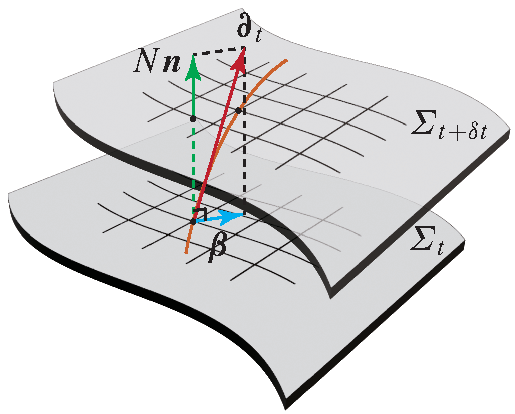
\includegraphics{Figures/foliation.pdf}
	\caption{A foliation of the spacetime. There are time vector $\timevec$, normal evolution vector $N\bm{n}$, and shift vector $\shiftvec$ satisfying $\timevec = N\bm{n} + \shiftvec$ between the two hypersurfaces $\Sigma_t$, $\Sigma_{t+\delta t}$.}
	\label{fig:foliation}
\end{figure}

From this, it is possible to calculate the next spatial metric from the initial condition of the space at a specific time. This is done in a similar way as in Newtonian classical mechanics, given the initial position and velocity of an object, the position and velocity at the next time can be calculated using the acceleration due to the force acting on the object. However, unlike in Newtonian mechanics, the initial value must satisfy certain specific conditions. Therefore, the calculation is made by first constructing the initial data, selecting the appropriate coordinates, and then evolving it from the numerical method.

\begin{figure}[H]
	\centering
	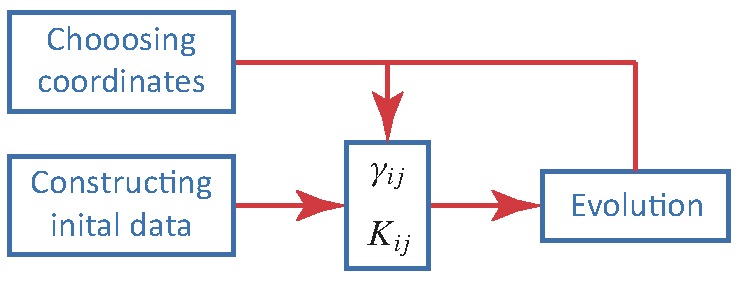
\includegraphics{Figures/scheme.pdf}
	\caption{A brief schema of numerical relativity.}
	\label{fig:scheme}
\end{figure}

In this work, we try to numerically evolve the Schwarzschild metric from its initial conditions to understand the basic way of working with numerical relativity.

\section{Notation and conventions}
%\subsection{Sign conventions}
Throughout this report, we follows the ``Landau-Lifshitz Spacelike Convention''($- + + +$) as \parencite{misner1973gravitation}. Also we will adopt a units for measurements in which both the gravitational constant $G$ and the speed of light $c$ are assigned the values of one.

We denote the dimension 4 spacetime metric by $g_{ab}$, the dimension 3 spatial metric
by $\gamma_{ij}$. Also the dimension 4 objects associated with $g_{ab}$ are denoted with a superscript ${}^{(4)}$ in front of the symbol, objects related to $\gamma_{ij}$ carry no decorations.
% Chapter Template

\chapter{The ADM Equations} % Main chapter title

\label{Chapter2} % Change X to a consecutive number; for referencing this chapter elsewhere, use \ref{ChapterX}



\section{Introduction}

In this chapter, we present how Einstein's equations can be decomposed into two constraints and two evolution equations. The development in this chapter follows \parencite{gourgoulhon20123+}.

\section{The Einstein Equation}
\emph{Einstein's equation} is
\begin{equation}
	\label{eq:einstein_equation}
	\dmf \bm{R} - \frac{1}{2}\dmf R\bm{g} = 8 \pi \bm{T}.
\end{equation}
We limit cosmological constant $\Lambda = 0$.

\section{Constraint equations}

Let's start with the \emph{Gauss relation}
\begin{equation}
	\label{eq:gauss_relation}
	\gamma^\mu _\alpha \gamma ^\nu_\beta \gamma^\gamma_\rho \gamma^\sigma_\delta \dmf R^\rho_{\sigma \mu \nu} = R^\gamma_{\delta\alpha\beta} + K^\gamma_\alpha K_{\delta\beta} - K^\gamma_\beta K_{\alpha\delta}.
\end{equation}
We can obtain \emph{scalar Gauss relation}
\begin{equation}
	\label{eq:scalar_gauss_relation}
	\dmf R + 2 \dmf R_{\mu\nu}n^\mu n^\nu = R + K^2 - K_{ij}K^{ij}
\end{equation}
by contract the Gauss relation Eq. (\ref{eq:gauss_relation}) on the indices $\gamma$ and $\alpha$ and use $\gamma^\mu_\alpha \gamma^\alpha_\rho = \gamma^\mu_\rho=\delta^\mu_\rho+n^\mu n_\rho$, and take its trace with respect to $\bm{\gamma}$.

From Eq. (\ref{eq:einstein_equation}), after full projection perpendicular to hypersurface $\Sigma_t$, we get
\begin{equation}
	\label{eq:bilinear_einstein_equation}
	\dmf \bm{R}(\bm{n}, \bm{n}) + \frac{1}{2}\dmf R = 8\pi \bm{T}(\bm{n}, \bm{n}) =: 8\pi E
\end{equation}
since $\bm{g}(\bm{n}, \bm{n}) = -1$. By combining Eq. (\ref{eq:scalar_gauss_relation}), (\ref{eq:bilinear_einstein_equation}), we get
\begin{equation}
	R+K^2 - K_{ij}^{ij} = 16\pi E
\end{equation}
which is called the \emph{Hamiltonian constraint}.

Now let us project Eq. (\ref{eq:einstein_equation}) onto $\Sigma_t$ and normal $\bm{n}$,
\begin{equation}
	\label{eq:mixed_einstein}
	\dmf \bm{R}(\bm{n}, \vec{\bm{\gamma}}(.)) - \frac{1}{2} \dmf R \bm{g}(\bm{n}, \vec{\bm{\gamma}}(.)) = 8\pi \bm{T}(\bm{n}, \vec{\bm{\gamma}}(.)).
\end{equation}

We can use \emph{Codazzi relation}
\begin{equation}
	\label{eq:codazzi_relation}
	\gamma^\gamma_\rho n^\sigma \gamma^\mu_\alpha\gamma^\nu_\beta \dmf R^\rho_{\sigma \mu \nu} = D_\beta K^\gamma_\alpha - D_\alpha K^\gamma_\beta
\end{equation}
to get \emph{contracted Codazzi relation}
\begin{equation}
	\gamma^\mu_\alpha n^\nu \dmf R_{\mu \nu} = D_\alpha K - D_\mu K^\mu _\alpha
\end{equation}
by contracting the Eq. (\ref{eq:codazzi_relation}) on the indices $\alpha$ and $\gamma$.

Since $\bm{g}(\bm{n}, \vec{\bm{\gamma}}(.))$ in Eq. (\ref{eq:mixed_einstein}) is equal to $0$ and by introducing \emph{matter momentum density} $\bm{p}:= - \bm{T}(\bm{n}, \vec{\bm{\gamma}}(.))$, we get
\begin{equation}
	\bm{D}\cdot \vec{\bm{K}} - \bm{D}K = 8 \pi \bm{p},
\end{equation}
or, in components,
\begin{equation}
	D_j K^j_i - D_i K = 8 \pi p_i
\end{equation}
which is called the \emph{momentum constraint}.



\section{Evolution equations}

Since we can write time vector in to sum of the normal evolution vector $\bm{m} := N\bm{n}$ and the shift vector $\shiftvec$,
\begin{equation}
	\label{eq:timevec}
	\timevec =: \bm{m} + \shiftvec,
\end{equation}
we can write
\begin{equation}
	\label{eq:lie_t}
	\mathcal{L}_{\bm{m}}\bm{T} = \mathcal{L}_{\timevec}\bm{T} - \mathcal{\shiftvec}\bm{T},
\end{equation}
for $\bm{T}$ be any tensor field tangent to $\Sigma_t$. Moreover, Lie derivative is simply obtained by taking the partial derivative of the vector components with respect to $t$. Therefore, Eq. (\ref{eq:lie_t}) can be written as
\begin{equation}
	\mathcal{L}_{\bm{m}} T^{i\cdots}_{j\cdots} = \qty(\pdv{t} - \mathcal{L}_{\shiftvec}) T^{i\cdots}_{j\cdots}.
\end{equation}

By applying it to extrinsic curvature
\begin{equation}
	\mathcal{L}_{\bm{m}} \bm{\gamma} = -2N \bm{K},
\end{equation}
it becomes
\begin{equation}
	\qty(\pdv{t} - \mathcal{L}_{\shiftvec})\gamma_{ij} = -2NK_{ij},
\end{equation}
which is called the \emph{evolution equation for the spatial metric}.

If we applying the operator $\vec{\bm{\gamma}}^{\ast}$ to the Einstein equation,
\begin{equation}
	\vec{\bm{\gamma}}^{\ast} \dmf \bm{R} = 8 \pi \qty( \vec{\bm{\gamma}}^{\ast} \bm{T} - \frac{1}{2}T \vec{\bm{\gamma}}^{\ast} \bm{g}).
\end{equation}
From the 3+1 decomposition of the Riemann tensor, we obtained
\begin{equation}
	\vec{\bm{\gamma}}^{\ast} \dmf \bm{R} = -\frac{1}{N} \mathcal{L}_{\bm{m}} \bm{K}- \frac{1}{N}\bm{D}\bm{D} N + \bm{R} + K \bm{K} - 2 \bm{K} \cdot \vec{\bm{K}}.
\end{equation}
Therefore
\begin{equation}
	\label{eq:full_projection}
	- \frac{1}{N} \mathcal{L}_{\bm{m}}\bm{K} - \frac{1}{N}\bm{D}\bm{D}N + \bm{R} + K \bm{K} - 2\bm{K}\cdot \vec{\bm{K}} = 8 \pi \qty [\bm{S} - \frac{1}{2}(S-E)\bm{\gamma}],
\end{equation}
where \emph{matter stress tensor} $\bm{S}:= \vec{\bm{\gamma}}^{\ast} \bm{T}$.

The result from property that the Lie derivative along $\bm{m}$ of any tensor field $\bm{T}$ tangent to $\Sigma_t$ is a tensor field tangent to $\Sigma_t$, Eq. (\ref{eq:full_projection}) can be written as
\begin{equation}
	\mathcal{L}_{\bm{m}}K_{ij} =  -D_i D_j N + N\qty{ R_{ij} + KK_{ij} - 2K_{ik}K^k_j +4\pi \qty[(S-E)\gamma_{ij}-2S_{ij}]}.
\end{equation}
From Eq. (\ref{eq:timevec}), we get \emph{evolution equation for the extrinsic curvature}
\begin{equation}
	\qty(\pdv{t} - \mathcal{L}_{\shiftvec})K_{ij} = -D_i D_j N + N\qty{ R_{ij} + KK_{ij} - 2K_{ik}K^k_j +4\pi \qty[(S-E)\gamma_{ij}-2S_{ij}]}.
\end{equation}

\section{Summary}
In this chapter, we obtained
the \emph{Hamiltonian constraint}
\begin{equation}
	\label{eq:hamiltonian_constraint}
	R+K^2-K_{ij}K^{ij} = 16\pi E,
\end{equation}
the \emph{momentum constraint}
\begin{equation}
	\label{eq:momentum_constraint}
	D_j K^j_i - D_i K = 8 \pi p_i,
\end{equation}
the \emph{evolution equation for the spatial metric}
\begin{equation}
	\label{eq:evolution_spatial}
\qty(\pdv{t} - \mathcal{L}_{\shiftvec})\gamma_{ij} = -2NK_{ij},
\end{equation}
and the \emph{evolution equation for the extrinsic curvature}
\begin{equation}
	\label{eq:evoultion_extrinsic}
	\qty(\pdv{t} - \mathcal{L}_{\shiftvec})K_{ij} = -D_i D_j N + N\qty{ R_{ij} + KK_{ij} - 2K_{ik}K^k_j +4\pi \qty[(S-E)\gamma_{ij}-2S_{ij}]}.
\end{equation}

%In ADM equations, the spacetime metric can be written as
%$$
%\dd{s^2} = -N^2 \dd{t^2}+\gamma_{ij} \qty(\dd{x^i} + \beta^i\dd{t}) \qty(\dd{x^j}+\beta^j \dd{t}).
%$$


% Chapter Template

\chapter{Numerical simulation} % Main chapter title

\label{Chapter3} % Change X to a consecutive number; for referencing this chapter elsewhere, use \ref{ChapterX}

\section{Introduction}

In this chapter, we describe the initial data set required prior to simulation, the numerical method for evolution, and the results.

\section{Schwarzschild black hole}
\subsection{Types of black holes}
Accordingly to the No-Hair theorem, all black holes solutions of the Einstein-Maxwell equation of electromagnetism in general relativity can be completely characterized by their observable classical parameters mass, electric charge and angular momentum.

The schwarzschild metric describes the spacetime geometry exterior to any spherical collapsing body. Kerr metric describes the geometry of empty spacetime around a rotating uncharged axially-symmetric black hole with quasi-spherical event horizon. There are also the Reissner-Nordström metric and the Kerr-Newman metric that describe charged black holes\parencite{vindana2018simulation, wald2010general}. In Table~\ref{tab:typeofblackholes}, it can be seen that the types of black holes are classified according to angular momentum and charge.
\begin{table}[H]
	\caption{Classifications of black holes.}
	\label{tab:typeofblackholes}
	\centering
	\begin{tabular}{c | c c}
		\toprule
		 & \textbf{Non-rotating} ($J=0$) & \textbf{Rotating} ($J>0$) \\
		\midrule
		\textbf{Uncharged} ($Q=0$) & Schwarzschild & Kerr\\
		\textbf{Charged}	($Q\neq0$) & Reissner-Nordström & Kerr-Newman\\
		\bottomrule
	\end{tabular}
\end{table}

\subsection{Isotropic coordinate}

In this report, we choose the simplest form, the Schwarzschild black hole. The original form of the Schwarzschild metric is
\begin{equation}
	\dd{s^2} = - \qty(1 - \frac{2M}{r}) \dd{t^2} + \qty(1 - \frac{2M}{r})^{-1}\dd{r^2}+r^2\qty(\dd{\theta^2}+\sin^2\theta\dd{\phi^2}).
\end{equation}
When $r$ goes $2M$, $g_{rr}$ diverges. However, this is just a coordinate singularity, like the problem that occurs at the north and south poles in the spherical coordinate system\parencite{zee2013einstein}. This can be solved by choosing another coordinate system, such as the Kruskal coordinate system.

We can avoid coordinate singularity at $r=2M$ by adopting an isotropic coordinate system by substituting $r=\bar{r}(1+M/2\bar{r})^2$, we get
\begin{equation}
	\dd{s^2} = - \qty(\frac{1-M/(2\bar{r})}{1+M/(2\bar{r})})^2 \dd{t^2} + \qty(1 + \frac{M}{2\bar{r}})^{4}\qty(\dd{\bar{r}^2}+\bar{r}^2\dd{\theta^2}+\bar{r}^2\sin^2\theta\dd{\phi^2}).
\end{equation}
This coordinate system describes the area outside the event horizon $\bar{r}=M/2$. The reason for using this coordinate system is as follows.
\begin{enumerate}
	\item A spatial metric is numerically valid in any space where $r>M/2$.
	\item Since spatial metrics are flat, they can be replaced with Cartesian coordinates, which is more useful for numerical calculations\parencite{brugmann1996adaptive}.
\end{enumerate}
So, in practice we use metric:
\begin{equation}
	\dd{s^2} = - \qty(\frac{1-M/(2r)}{1+M/(2r)})^2 \dd{t^2} + \qty(1 + \frac{M}{2r})^{4}\qty(\dd{x^2}+\dd{y^2}+\dd{z^2}),
\end{equation}
where $r = \sqrt{x^2 + y^2 + z^2}$.

\section{Gauge conditions}
Eq. (\ref{eq:hamiltonian_constraint})-(\ref{eq:evoultion_extrinsic}) does not contain any time derivative of lapse function $N$ nor of the shift vector $\shiftvec$. This means that $N$ and $\shiftvec$ are not dynamical variables. Therefore, we may choose the lapse and shift freely, without changing the physical solution $g$ of the Einstein equation\parencite{gourgoulhon20123+}.

In this simulation, we choose the lapse function and the shift vector
\begin{equation}
	N = \frac{1-M/(2r)}{1+M/(2r)}, \qquad \shiftvec = 0.
\end{equation}

\section{Initial data}
After 3+1 decomposition, we should evolve forward in time some initial data. Instead of solving Hamiltonian and momentum constraint, we use well-known initial data from isotropic coordinates of Schwarzshcild metric. So the initial spatial metric becomes $\gamma_{ij}=(1+M/(2r))^4\delta_{ij}$ and the initial extrinsic curvature becomes $K_{ij} = -\frac{1}{2}\mathcal{L}_{\bm{n}}\gamma_{ij} = 0$.

We will show that these data satisfies Eq. (\ref{eq:hamiltonian_constraint}, \ref{eq:momentum_constraint}). Since $E$ and $p_i$ are all $0$ in vacuum space and $K_{ij}=0$, the momentum constraint is naturally satisfied. Now, to satisfy the hamiltonian constraint, we need to show that the 3-metric Ricci scalar $R$ is $0$. Let's use a spherical coordinate system here. The non-vanishing Ricci tensor is:
\begin{align}
	R_{rr} &= - \frac{8 M}{r \left(M + 2 r\right)^{2}},\\
	R_{\theta\theta} &= \frac{4 M r}{\left(M + 2 r\right)^{2}},\\
	R_{\phi\phi} &= \frac{4 M r \sin^{2}{\left(\theta \right)}}{\left(M + 2 r\right)^{2}}.
\end{align}
Therefore, it can be seen that the 3-metric Ricci scalar $R = \gamma^{ij}R_{ij} = 0$, and it can be confirmed that the given constraint condition is well satisfied.

\section{Numerical methods}
\subsection{Finite difference method}
This simulation uses the finite difference method. The Taylor expansion of the function $f(x)$ in $x_0$ is
\begin{equation}
	f(x_0 + h) = f(x_0) + \frac{f'(x_0)}{1!}h + \frac{f^{(2)}(x_0)}{2!}h^2 + \cdots + \frac{f^{(n)}(x_0)}{n!}h^n+ \cdots .
\end{equation}
Arranging this, we get
\begin{equation}
	\begin{aligned}
		\frac{f(x_0 + h) - f(x_0)}{h} &= f'(x_0) + \frac{f^{(2)}(x_0)}{2!}h + \cdots \\
		&= f'(x_0) + \mathcal{O}(h).
	\end{aligned}
\end{equation}
Accuracy is on the order of $\mathcal{O}(h)$.

The central difference method selects the function value from $x-h$ and $x+h$, respectively, and has a more accurate error of $\mathcal{O}(h^2)$.
\begin{equation}
	f'(x_0) = \frac{f(x+ h) - f(x - h)}{2h} + \mathcal{O}(h^2).
\end{equation}

\subsection{Boundary condition}

The isotropic coordinates of the schwarzschild metric only describe the region outside the black hole horizon, i.e. $r=\frac{M}{2}$. Therefore, $\gamma_{ij}$ and $K_{ij}$ were fixed in the region of $r\le \frac{M}{2}$.

At the boundary outside the grid, the physical quantity at the corresponding point was calculated using linear extrapolation. For example, when we need to find the derivative at $f_i$,
\begin{align}
	(\partial f)_{i - 2} &= \frac{f_{i - 1} - f_{i - 3}}{2h},\\
	(\partial f)_{i - 1} &= \frac{f_{i} - f_{i - 2}}{2h}.
\end{align}

Therefore, we get
\begin{equation}
	\begin{aligned}
			(\partial f)_{i} &= \frac{f_{i - 1} - f_{i - 3}}{2h}\\
			&= \frac{2f_i - f_{i - 1} - 2f_{i - 2} + f_{i - 3}}{2h}.
	\end{aligned}
\end{equation}

Alternatively, there is a way to use a fixed value at the grid boundary, as well as at the black hole horizon.

\subsection{Inverse matrix}

Cofactors were used to find the inverse matrix. See Appendix \ref{AppendixA}.

\section{Grid setting}

The size of the grid is $100^3$, the mass of the black hole is $0.2M$, and the grid distance is $0.01M$. Thus, the horizon of a black hole corresponds to $0.1 M$, i.e. the surface of a sphere with a radius of 10 grids.

\section{Result}

The results obtained at first do not change with time as shown in Fig. \ref{fig:0_data0}.
\begin{figure}[H]
	\centering
	%% Creator: Matplotlib, PGF backend
%%
%% To include the figure in your LaTeX document, write
%%   \input{<filename>.pgf}
%%
%% Make sure the required packages are loaded in your preamble
%%   \usepackage{pgf}
%%
%% Also ensure that all the required font packages are loaded; for instance,
%% the lmodern package is sometimes necessary when using math font.
%%   \usepackage{lmodern}
%%
%% Figures using additional raster images can only be included by \input if
%% they are in the same directory as the main LaTeX file. For loading figures
%% from other directories you can use the `import` package
%%   \usepackage{import}
%%
%% and then include the figures with
%%   \import{<path to file>}{<filename>.pgf}
%%
%% Matplotlib used the following preamble
%%   \usepackage{fontspec}
%%   \setmainfont{DejaVuSerif.ttf}[Path=\detokenize{C:/boj/venv/Lib/site-packages/matplotlib/mpl-data/fonts/ttf/}]
%%   \setsansfont{DejaVuSans.ttf}[Path=\detokenize{C:/boj/venv/Lib/site-packages/matplotlib/mpl-data/fonts/ttf/}]
%%   \setmonofont{DejaVuSansMono.ttf}[Path=\detokenize{C:/boj/venv/Lib/site-packages/matplotlib/mpl-data/fonts/ttf/}]
%%
\begingroup%
\makeatletter%
\begin{pgfpicture}%
\pgfpathrectangle{\pgfpointorigin}{\pgfqpoint{4.000000in}{4.000000in}}%
\pgfusepath{use as bounding box, clip}%
\begin{pgfscope}%
\pgfsetbuttcap%
\pgfsetmiterjoin%
\definecolor{currentfill}{rgb}{1.000000,1.000000,1.000000}%
\pgfsetfillcolor{currentfill}%
\pgfsetlinewidth{0.000000pt}%
\definecolor{currentstroke}{rgb}{1.000000,1.000000,1.000000}%
\pgfsetstrokecolor{currentstroke}%
\pgfsetdash{}{0pt}%
\pgfpathmoveto{\pgfqpoint{0.000000in}{0.000000in}}%
\pgfpathlineto{\pgfqpoint{4.000000in}{0.000000in}}%
\pgfpathlineto{\pgfqpoint{4.000000in}{4.000000in}}%
\pgfpathlineto{\pgfqpoint{0.000000in}{4.000000in}}%
\pgfpathlineto{\pgfqpoint{0.000000in}{0.000000in}}%
\pgfpathclose%
\pgfusepath{fill}%
\end{pgfscope}%
\begin{pgfscope}%
\pgfsetbuttcap%
\pgfsetmiterjoin%
\definecolor{currentfill}{rgb}{1.000000,1.000000,1.000000}%
\pgfsetfillcolor{currentfill}%
\pgfsetlinewidth{0.000000pt}%
\definecolor{currentstroke}{rgb}{0.000000,0.000000,0.000000}%
\pgfsetstrokecolor{currentstroke}%
\pgfsetstrokeopacity{0.000000}%
\pgfsetdash{}{0pt}%
\pgfpathmoveto{\pgfqpoint{0.000000in}{0.300000in}}%
\pgfpathlineto{\pgfqpoint{3.400000in}{0.300000in}}%
\pgfpathlineto{\pgfqpoint{3.400000in}{3.700000in}}%
\pgfpathlineto{\pgfqpoint{0.000000in}{3.700000in}}%
\pgfpathlineto{\pgfqpoint{0.000000in}{0.300000in}}%
\pgfpathclose%
\pgfusepath{fill}%
\end{pgfscope}%
\begin{pgfscope}%
\pgfsetbuttcap%
\pgfsetmiterjoin%
\definecolor{currentfill}{rgb}{0.950000,0.950000,0.950000}%
\pgfsetfillcolor{currentfill}%
\pgfsetfillopacity{0.500000}%
\pgfsetlinewidth{1.003750pt}%
\definecolor{currentstroke}{rgb}{0.950000,0.950000,0.950000}%
\pgfsetstrokecolor{currentstroke}%
\pgfsetstrokeopacity{0.500000}%
\pgfsetdash{}{0pt}%
\pgfpathmoveto{\pgfqpoint{0.256723in}{1.138331in}}%
\pgfpathlineto{\pgfqpoint{1.379514in}{2.079477in}}%
\pgfpathlineto{\pgfqpoint{1.363907in}{3.436777in}}%
\pgfpathlineto{\pgfqpoint{0.187384in}{2.578205in}}%
\pgfusepath{stroke,fill}%
\end{pgfscope}%
\begin{pgfscope}%
\pgfsetbuttcap%
\pgfsetmiterjoin%
\definecolor{currentfill}{rgb}{0.900000,0.900000,0.900000}%
\pgfsetfillcolor{currentfill}%
\pgfsetfillopacity{0.500000}%
\pgfsetlinewidth{1.003750pt}%
\definecolor{currentstroke}{rgb}{0.900000,0.900000,0.900000}%
\pgfsetstrokecolor{currentstroke}%
\pgfsetstrokeopacity{0.500000}%
\pgfsetdash{}{0pt}%
\pgfpathmoveto{\pgfqpoint{1.379514in}{2.079477in}}%
\pgfpathlineto{\pgfqpoint{3.181193in}{1.555800in}}%
\pgfpathlineto{\pgfqpoint{3.245489in}{2.959851in}}%
\pgfpathlineto{\pgfqpoint{1.363907in}{3.436777in}}%
\pgfusepath{stroke,fill}%
\end{pgfscope}%
\begin{pgfscope}%
\pgfsetbuttcap%
\pgfsetmiterjoin%
\definecolor{currentfill}{rgb}{0.925000,0.925000,0.925000}%
\pgfsetfillcolor{currentfill}%
\pgfsetfillopacity{0.500000}%
\pgfsetlinewidth{1.003750pt}%
\definecolor{currentstroke}{rgb}{0.925000,0.925000,0.925000}%
\pgfsetstrokecolor{currentstroke}%
\pgfsetstrokeopacity{0.500000}%
\pgfsetdash{}{0pt}%
\pgfpathmoveto{\pgfqpoint{0.256723in}{1.138331in}}%
\pgfpathlineto{\pgfqpoint{2.166591in}{0.514568in}}%
\pgfpathlineto{\pgfqpoint{3.181193in}{1.555800in}}%
\pgfpathlineto{\pgfqpoint{1.379514in}{2.079477in}}%
\pgfusepath{stroke,fill}%
\end{pgfscope}%
\begin{pgfscope}%
\pgfsetrectcap%
\pgfsetroundjoin%
\pgfsetlinewidth{0.803000pt}%
\definecolor{currentstroke}{rgb}{0.000000,0.000000,0.000000}%
\pgfsetstrokecolor{currentstroke}%
\pgfsetdash{}{0pt}%
\pgfpathmoveto{\pgfqpoint{0.256723in}{1.138331in}}%
\pgfpathlineto{\pgfqpoint{2.166591in}{0.514568in}}%
\pgfusepath{stroke}%
\end{pgfscope}%
\begin{pgfscope}%
\definecolor{textcolor}{rgb}{0.000000,0.000000,0.000000}%
\pgfsetstrokecolor{textcolor}%
\pgfsetfillcolor{textcolor}%
\pgftext[x=0.810290in, y=0.356812in, left, base,rotate=341.912962]{\color{textcolor}\sffamily\fontsize{10.000000}{12.000000}\selectfont \(\displaystyle y/M\)}%
\end{pgfscope}%
\begin{pgfscope}%
\pgfsetbuttcap%
\pgfsetroundjoin%
\pgfsetlinewidth{0.803000pt}%
\definecolor{currentstroke}{rgb}{0.690196,0.690196,0.690196}%
\pgfsetstrokecolor{currentstroke}%
\pgfsetdash{}{0pt}%
\pgfpathmoveto{\pgfqpoint{0.532270in}{1.048338in}}%
\pgfpathlineto{\pgfqpoint{1.640436in}{2.003637in}}%
\pgfpathlineto{\pgfqpoint{1.635908in}{3.367833in}}%
\pgfusepath{stroke}%
\end{pgfscope}%
\begin{pgfscope}%
\pgfsetbuttcap%
\pgfsetroundjoin%
\pgfsetlinewidth{0.803000pt}%
\definecolor{currentstroke}{rgb}{0.690196,0.690196,0.690196}%
\pgfsetstrokecolor{currentstroke}%
\pgfsetdash{}{0pt}%
\pgfpathmoveto{\pgfqpoint{0.856393in}{0.942479in}}%
\pgfpathlineto{\pgfqpoint{1.946929in}{1.914552in}}%
\pgfpathlineto{\pgfqpoint{1.955629in}{3.286793in}}%
\pgfusepath{stroke}%
\end{pgfscope}%
\begin{pgfscope}%
\pgfsetbuttcap%
\pgfsetroundjoin%
\pgfsetlinewidth{0.803000pt}%
\definecolor{currentstroke}{rgb}{0.690196,0.690196,0.690196}%
\pgfsetstrokecolor{currentstroke}%
\pgfsetdash{}{0pt}%
\pgfpathmoveto{\pgfqpoint{1.186482in}{0.834672in}}%
\pgfpathlineto{\pgfqpoint{2.258592in}{1.823963in}}%
\pgfpathlineto{\pgfqpoint{2.280979in}{3.204326in}}%
\pgfusepath{stroke}%
\end{pgfscope}%
\begin{pgfscope}%
\pgfsetbuttcap%
\pgfsetroundjoin%
\pgfsetlinewidth{0.803000pt}%
\definecolor{currentstroke}{rgb}{0.690196,0.690196,0.690196}%
\pgfsetstrokecolor{currentstroke}%
\pgfsetdash{}{0pt}%
\pgfpathmoveto{\pgfqpoint{1.522704in}{0.724862in}}%
\pgfpathlineto{\pgfqpoint{2.575557in}{1.731834in}}%
\pgfpathlineto{\pgfqpoint{2.612106in}{3.120395in}}%
\pgfusepath{stroke}%
\end{pgfscope}%
\begin{pgfscope}%
\pgfsetbuttcap%
\pgfsetroundjoin%
\pgfsetlinewidth{0.803000pt}%
\definecolor{currentstroke}{rgb}{0.690196,0.690196,0.690196}%
\pgfsetstrokecolor{currentstroke}%
\pgfsetdash{}{0pt}%
\pgfpathmoveto{\pgfqpoint{1.865230in}{0.612993in}}%
\pgfpathlineto{\pgfqpoint{2.897959in}{1.638125in}}%
\pgfpathlineto{\pgfqpoint{2.949166in}{3.034960in}}%
\pgfusepath{stroke}%
\end{pgfscope}%
\begin{pgfscope}%
\pgfsetrectcap%
\pgfsetroundjoin%
\pgfsetlinewidth{0.803000pt}%
\definecolor{currentstroke}{rgb}{0.000000,0.000000,0.000000}%
\pgfsetstrokecolor{currentstroke}%
\pgfsetdash{}{0pt}%
\pgfpathmoveto{\pgfqpoint{0.541923in}{1.056659in}}%
\pgfpathlineto{\pgfqpoint{0.512921in}{1.031658in}}%
\pgfusepath{stroke}%
\end{pgfscope}%
\begin{pgfscope}%
\definecolor{textcolor}{rgb}{0.000000,0.000000,0.000000}%
\pgfsetstrokecolor{textcolor}%
\pgfsetfillcolor{textcolor}%
\pgftext[x=0.427840in,y=0.828860in,,top]{\color{textcolor}\sffamily\fontsize{10.000000}{12.000000}\selectfont \(\displaystyle {\ensuremath{-}2}\)}%
\end{pgfscope}%
\begin{pgfscope}%
\pgfsetrectcap%
\pgfsetroundjoin%
\pgfsetlinewidth{0.803000pt}%
\definecolor{currentstroke}{rgb}{0.000000,0.000000,0.000000}%
\pgfsetstrokecolor{currentstroke}%
\pgfsetdash{}{0pt}%
\pgfpathmoveto{\pgfqpoint{0.865900in}{0.950953in}}%
\pgfpathlineto{\pgfqpoint{0.837338in}{0.925494in}}%
\pgfusepath{stroke}%
\end{pgfscope}%
\begin{pgfscope}%
\definecolor{textcolor}{rgb}{0.000000,0.000000,0.000000}%
\pgfsetstrokecolor{textcolor}%
\pgfsetfillcolor{textcolor}%
\pgftext[x=0.752336in,y=0.720558in,,top]{\color{textcolor}\sffamily\fontsize{10.000000}{12.000000}\selectfont \(\displaystyle {\ensuremath{-}1}\)}%
\end{pgfscope}%
\begin{pgfscope}%
\pgfsetrectcap%
\pgfsetroundjoin%
\pgfsetlinewidth{0.803000pt}%
\definecolor{currentstroke}{rgb}{0.000000,0.000000,0.000000}%
\pgfsetstrokecolor{currentstroke}%
\pgfsetdash{}{0pt}%
\pgfpathmoveto{\pgfqpoint{1.195836in}{0.843303in}}%
\pgfpathlineto{\pgfqpoint{1.167735in}{0.817372in}}%
\pgfusepath{stroke}%
\end{pgfscope}%
\begin{pgfscope}%
\definecolor{textcolor}{rgb}{0.000000,0.000000,0.000000}%
\pgfsetstrokecolor{textcolor}%
\pgfsetfillcolor{textcolor}%
\pgftext[x=1.082828in,y=0.610254in,,top]{\color{textcolor}\sffamily\fontsize{10.000000}{12.000000}\selectfont \(\displaystyle {0}\)}%
\end{pgfscope}%
\begin{pgfscope}%
\pgfsetrectcap%
\pgfsetroundjoin%
\pgfsetlinewidth{0.803000pt}%
\definecolor{currentstroke}{rgb}{0.000000,0.000000,0.000000}%
\pgfsetstrokecolor{currentstroke}%
\pgfsetdash{}{0pt}%
\pgfpathmoveto{\pgfqpoint{1.531896in}{0.733654in}}%
\pgfpathlineto{\pgfqpoint{1.504278in}{0.707239in}}%
\pgfusepath{stroke}%
\end{pgfscope}%
\begin{pgfscope}%
\definecolor{textcolor}{rgb}{0.000000,0.000000,0.000000}%
\pgfsetstrokecolor{textcolor}%
\pgfsetfillcolor{textcolor}%
\pgftext[x=1.419486in,y=0.497893in,,top]{\color{textcolor}\sffamily\fontsize{10.000000}{12.000000}\selectfont \(\displaystyle {1}\)}%
\end{pgfscope}%
\begin{pgfscope}%
\pgfsetrectcap%
\pgfsetroundjoin%
\pgfsetlinewidth{0.803000pt}%
\definecolor{currentstroke}{rgb}{0.000000,0.000000,0.000000}%
\pgfsetstrokecolor{currentstroke}%
\pgfsetdash{}{0pt}%
\pgfpathmoveto{\pgfqpoint{1.874253in}{0.621950in}}%
\pgfpathlineto{\pgfqpoint{1.847142in}{0.595038in}}%
\pgfusepath{stroke}%
\end{pgfscope}%
\begin{pgfscope}%
\definecolor{textcolor}{rgb}{0.000000,0.000000,0.000000}%
\pgfsetstrokecolor{textcolor}%
\pgfsetfillcolor{textcolor}%
\pgftext[x=1.762484in,y=0.383416in,,top]{\color{textcolor}\sffamily\fontsize{10.000000}{12.000000}\selectfont \(\displaystyle {2}\)}%
\end{pgfscope}%
\begin{pgfscope}%
\pgfsetrectcap%
\pgfsetroundjoin%
\pgfsetlinewidth{0.803000pt}%
\definecolor{currentstroke}{rgb}{0.000000,0.000000,0.000000}%
\pgfsetstrokecolor{currentstroke}%
\pgfsetdash{}{0pt}%
\pgfpathmoveto{\pgfqpoint{3.181193in}{1.555800in}}%
\pgfpathlineto{\pgfqpoint{2.166591in}{0.514568in}}%
\pgfusepath{stroke}%
\end{pgfscope}%
\begin{pgfscope}%
\definecolor{textcolor}{rgb}{0.000000,0.000000,0.000000}%
\pgfsetstrokecolor{textcolor}%
\pgfsetfillcolor{textcolor}%
\pgftext[x=2.991868in, y=0.538204in, left, base,rotate=45.742112]{\color{textcolor}\sffamily\fontsize{10.000000}{12.000000}\selectfont \(\displaystyle x/M\)}%
\end{pgfscope}%
\begin{pgfscope}%
\pgfsetbuttcap%
\pgfsetroundjoin%
\pgfsetlinewidth{0.803000pt}%
\definecolor{currentstroke}{rgb}{0.690196,0.690196,0.690196}%
\pgfsetstrokecolor{currentstroke}%
\pgfsetdash{}{0pt}%
\pgfpathmoveto{\pgfqpoint{0.378776in}{2.717874in}}%
\pgfpathlineto{\pgfqpoint{0.438794in}{1.290947in}}%
\pgfpathlineto{\pgfqpoint{2.331728in}{0.684039in}}%
\pgfusepath{stroke}%
\end{pgfscope}%
\begin{pgfscope}%
\pgfsetbuttcap%
\pgfsetroundjoin%
\pgfsetlinewidth{0.803000pt}%
\definecolor{currentstroke}{rgb}{0.690196,0.690196,0.690196}%
\pgfsetstrokecolor{currentstroke}%
\pgfsetdash{}{0pt}%
\pgfpathmoveto{\pgfqpoint{0.593633in}{2.874667in}}%
\pgfpathlineto{\pgfqpoint{0.643456in}{1.462498in}}%
\pgfpathlineto{\pgfqpoint{2.517072in}{0.874247in}}%
\pgfusepath{stroke}%
\end{pgfscope}%
\begin{pgfscope}%
\pgfsetbuttcap%
\pgfsetroundjoin%
\pgfsetlinewidth{0.803000pt}%
\definecolor{currentstroke}{rgb}{0.690196,0.690196,0.690196}%
\pgfsetstrokecolor{currentstroke}%
\pgfsetdash{}{0pt}%
\pgfpathmoveto{\pgfqpoint{0.801817in}{3.026590in}}%
\pgfpathlineto{\pgfqpoint{0.842031in}{1.628948in}}%
\pgfpathlineto{\pgfqpoint{2.696618in}{1.058506in}}%
\pgfusepath{stroke}%
\end{pgfscope}%
\begin{pgfscope}%
\pgfsetbuttcap%
\pgfsetroundjoin%
\pgfsetlinewidth{0.803000pt}%
\definecolor{currentstroke}{rgb}{0.690196,0.690196,0.690196}%
\pgfsetstrokecolor{currentstroke}%
\pgfsetdash{}{0pt}%
\pgfpathmoveto{\pgfqpoint{1.003633in}{3.173865in}}%
\pgfpathlineto{\pgfqpoint{1.034788in}{1.790520in}}%
\pgfpathlineto{\pgfqpoint{2.870636in}{1.237091in}}%
\pgfusepath{stroke}%
\end{pgfscope}%
\begin{pgfscope}%
\pgfsetbuttcap%
\pgfsetroundjoin%
\pgfsetlinewidth{0.803000pt}%
\definecolor{currentstroke}{rgb}{0.690196,0.690196,0.690196}%
\pgfsetstrokecolor{currentstroke}%
\pgfsetdash{}{0pt}%
\pgfpathmoveto{\pgfqpoint{1.199368in}{3.316705in}}%
\pgfpathlineto{\pgfqpoint{1.221977in}{1.947426in}}%
\pgfpathlineto{\pgfqpoint{3.039375in}{1.410260in}}%
\pgfusepath{stroke}%
\end{pgfscope}%
\begin{pgfscope}%
\pgfsetrectcap%
\pgfsetroundjoin%
\pgfsetlinewidth{0.803000pt}%
\definecolor{currentstroke}{rgb}{0.000000,0.000000,0.000000}%
\pgfsetstrokecolor{currentstroke}%
\pgfsetdash{}{0pt}%
\pgfpathmoveto{\pgfqpoint{2.315783in}{0.689151in}}%
\pgfpathlineto{\pgfqpoint{2.363659in}{0.673801in}}%
\pgfusepath{stroke}%
\end{pgfscope}%
\begin{pgfscope}%
\definecolor{textcolor}{rgb}{0.000000,0.000000,0.000000}%
\pgfsetstrokecolor{textcolor}%
\pgfsetfillcolor{textcolor}%
\pgftext[x=2.509251in,y=0.499164in,,top]{\color{textcolor}\sffamily\fontsize{10.000000}{12.000000}\selectfont \(\displaystyle {\ensuremath{-}2}\)}%
\end{pgfscope}%
\begin{pgfscope}%
\pgfsetrectcap%
\pgfsetroundjoin%
\pgfsetlinewidth{0.803000pt}%
\definecolor{currentstroke}{rgb}{0.000000,0.000000,0.000000}%
\pgfsetstrokecolor{currentstroke}%
\pgfsetdash{}{0pt}%
\pgfpathmoveto{\pgfqpoint{2.501302in}{0.879199in}}%
\pgfpathlineto{\pgfqpoint{2.548651in}{0.864332in}}%
\pgfusepath{stroke}%
\end{pgfscope}%
\begin{pgfscope}%
\definecolor{textcolor}{rgb}{0.000000,0.000000,0.000000}%
\pgfsetstrokecolor{textcolor}%
\pgfsetfillcolor{textcolor}%
\pgftext[x=2.691891in,y=0.692432in,,top]{\color{textcolor}\sffamily\fontsize{10.000000}{12.000000}\selectfont \(\displaystyle {\ensuremath{-}1}\)}%
\end{pgfscope}%
\begin{pgfscope}%
\pgfsetrectcap%
\pgfsetroundjoin%
\pgfsetlinewidth{0.803000pt}%
\definecolor{currentstroke}{rgb}{0.000000,0.000000,0.000000}%
\pgfsetstrokecolor{currentstroke}%
\pgfsetdash{}{0pt}%
\pgfpathmoveto{\pgfqpoint{2.681020in}{1.063304in}}%
\pgfpathlineto{\pgfqpoint{2.727852in}{1.048899in}}%
\pgfusepath{stroke}%
\end{pgfscope}%
\begin{pgfscope}%
\definecolor{textcolor}{rgb}{0.000000,0.000000,0.000000}%
\pgfsetstrokecolor{textcolor}%
\pgfsetfillcolor{textcolor}%
\pgftext[x=2.868814in,y=0.879651in,,top]{\color{textcolor}\sffamily\fontsize{10.000000}{12.000000}\selectfont \(\displaystyle {0}\)}%
\end{pgfscope}%
\begin{pgfscope}%
\pgfsetrectcap%
\pgfsetroundjoin%
\pgfsetlinewidth{0.803000pt}%
\definecolor{currentstroke}{rgb}{0.000000,0.000000,0.000000}%
\pgfsetstrokecolor{currentstroke}%
\pgfsetdash{}{0pt}%
\pgfpathmoveto{\pgfqpoint{2.855207in}{1.241742in}}%
\pgfpathlineto{\pgfqpoint{2.901530in}{1.227778in}}%
\pgfusepath{stroke}%
\end{pgfscope}%
\begin{pgfscope}%
\definecolor{textcolor}{rgb}{0.000000,0.000000,0.000000}%
\pgfsetstrokecolor{textcolor}%
\pgfsetfillcolor{textcolor}%
\pgftext[x=3.040285in,y=1.061101in,,top]{\color{textcolor}\sffamily\fontsize{10.000000}{12.000000}\selectfont \(\displaystyle {1}\)}%
\end{pgfscope}%
\begin{pgfscope}%
\pgfsetrectcap%
\pgfsetroundjoin%
\pgfsetlinewidth{0.803000pt}%
\definecolor{currentstroke}{rgb}{0.000000,0.000000,0.000000}%
\pgfsetstrokecolor{currentstroke}%
\pgfsetdash{}{0pt}%
\pgfpathmoveto{\pgfqpoint{3.024113in}{1.414771in}}%
\pgfpathlineto{\pgfqpoint{3.069937in}{1.401227in}}%
\pgfusepath{stroke}%
\end{pgfscope}%
\begin{pgfscope}%
\definecolor{textcolor}{rgb}{0.000000,0.000000,0.000000}%
\pgfsetstrokecolor{textcolor}%
\pgfsetfillcolor{textcolor}%
\pgftext[x=3.206553in,y=1.237045in,,top]{\color{textcolor}\sffamily\fontsize{10.000000}{12.000000}\selectfont \(\displaystyle {2}\)}%
\end{pgfscope}%
\begin{pgfscope}%
\pgfsetrectcap%
\pgfsetroundjoin%
\pgfsetlinewidth{0.803000pt}%
\definecolor{currentstroke}{rgb}{0.000000,0.000000,0.000000}%
\pgfsetstrokecolor{currentstroke}%
\pgfsetdash{}{0pt}%
\pgfpathmoveto{\pgfqpoint{3.181193in}{1.555800in}}%
\pgfpathlineto{\pgfqpoint{3.245489in}{2.959851in}}%
\pgfusepath{stroke}%
\end{pgfscope}%
\begin{pgfscope}%
\definecolor{textcolor}{rgb}{0.000000,0.000000,0.000000}%
\pgfsetstrokecolor{textcolor}%
\pgfsetfillcolor{textcolor}%
\pgftext[x=3.796647in, y=2.231502in, left, base,rotate=87.378092]{\color{textcolor}\sffamily\fontsize{10.000000}{12.000000}\selectfont \(\displaystyle \gamma_{ij}\)}%
\end{pgfscope}%
\begin{pgfscope}%
\pgfsetbuttcap%
\pgfsetroundjoin%
\pgfsetlinewidth{0.803000pt}%
\definecolor{currentstroke}{rgb}{0.690196,0.690196,0.690196}%
\pgfsetstrokecolor{currentstroke}%
\pgfsetdash{}{0pt}%
\pgfpathmoveto{\pgfqpoint{3.190658in}{1.762486in}}%
\pgfpathlineto{\pgfqpoint{1.377213in}{2.279641in}}%
\pgfpathlineto{\pgfqpoint{0.246531in}{1.349986in}}%
\pgfusepath{stroke}%
\end{pgfscope}%
\begin{pgfscope}%
\pgfsetbuttcap%
\pgfsetroundjoin%
\pgfsetlinewidth{0.803000pt}%
\definecolor{currentstroke}{rgb}{0.690196,0.690196,0.690196}%
\pgfsetstrokecolor{currentstroke}%
\pgfsetdash{}{0pt}%
\pgfpathmoveto{\pgfqpoint{3.199306in}{1.951335in}}%
\pgfpathlineto{\pgfqpoint{1.375111in}{2.462422in}}%
\pgfpathlineto{\pgfqpoint{0.237214in}{1.543467in}}%
\pgfusepath{stroke}%
\end{pgfscope}%
\begin{pgfscope}%
\pgfsetbuttcap%
\pgfsetroundjoin%
\pgfsetlinewidth{0.803000pt}%
\definecolor{currentstroke}{rgb}{0.690196,0.690196,0.690196}%
\pgfsetstrokecolor{currentstroke}%
\pgfsetdash{}{0pt}%
\pgfpathmoveto{\pgfqpoint{3.208058in}{2.142458in}}%
\pgfpathlineto{\pgfqpoint{1.372985in}{2.647298in}}%
\pgfpathlineto{\pgfqpoint{0.227780in}{1.739367in}}%
\pgfusepath{stroke}%
\end{pgfscope}%
\begin{pgfscope}%
\pgfsetbuttcap%
\pgfsetroundjoin%
\pgfsetlinewidth{0.803000pt}%
\definecolor{currentstroke}{rgb}{0.690196,0.690196,0.690196}%
\pgfsetstrokecolor{currentstroke}%
\pgfsetdash{}{0pt}%
\pgfpathmoveto{\pgfqpoint{3.216916in}{2.335897in}}%
\pgfpathlineto{\pgfqpoint{1.370835in}{2.834307in}}%
\pgfpathlineto{\pgfqpoint{0.218227in}{1.937732in}}%
\pgfusepath{stroke}%
\end{pgfscope}%
\begin{pgfscope}%
\pgfsetbuttcap%
\pgfsetroundjoin%
\pgfsetlinewidth{0.803000pt}%
\definecolor{currentstroke}{rgb}{0.690196,0.690196,0.690196}%
\pgfsetstrokecolor{currentstroke}%
\pgfsetdash{}{0pt}%
\pgfpathmoveto{\pgfqpoint{3.225883in}{2.531695in}}%
\pgfpathlineto{\pgfqpoint{1.368659in}{3.023484in}}%
\pgfpathlineto{\pgfqpoint{0.208554in}{2.138610in}}%
\pgfusepath{stroke}%
\end{pgfscope}%
\begin{pgfscope}%
\pgfsetbuttcap%
\pgfsetroundjoin%
\pgfsetlinewidth{0.803000pt}%
\definecolor{currentstroke}{rgb}{0.690196,0.690196,0.690196}%
\pgfsetstrokecolor{currentstroke}%
\pgfsetdash{}{0pt}%
\pgfpathmoveto{\pgfqpoint{3.234959in}{2.729893in}}%
\pgfpathlineto{\pgfqpoint{1.366458in}{3.214869in}}%
\pgfpathlineto{\pgfqpoint{0.198757in}{2.342047in}}%
\pgfusepath{stroke}%
\end{pgfscope}%
\begin{pgfscope}%
\pgfsetbuttcap%
\pgfsetroundjoin%
\pgfsetlinewidth{0.803000pt}%
\definecolor{currentstroke}{rgb}{0.690196,0.690196,0.690196}%
\pgfsetstrokecolor{currentstroke}%
\pgfsetdash{}{0pt}%
\pgfpathmoveto{\pgfqpoint{3.244147in}{2.930538in}}%
\pgfpathlineto{\pgfqpoint{1.364232in}{3.408499in}}%
\pgfpathlineto{\pgfqpoint{0.188834in}{2.548094in}}%
\pgfusepath{stroke}%
\end{pgfscope}%
\begin{pgfscope}%
\pgfsetrectcap%
\pgfsetroundjoin%
\pgfsetlinewidth{0.803000pt}%
\definecolor{currentstroke}{rgb}{0.000000,0.000000,0.000000}%
\pgfsetstrokecolor{currentstroke}%
\pgfsetdash{}{0pt}%
\pgfpathmoveto{\pgfqpoint{3.175434in}{1.766828in}}%
\pgfpathlineto{\pgfqpoint{3.221144in}{1.753792in}}%
\pgfusepath{stroke}%
\end{pgfscope}%
\begin{pgfscope}%
\definecolor{textcolor}{rgb}{0.000000,0.000000,0.000000}%
\pgfsetstrokecolor{textcolor}%
\pgfsetfillcolor{textcolor}%
\pgftext[x=3.445680in,y=1.798217in,,top]{\color{textcolor}\sffamily\fontsize{10.000000}{12.000000}\selectfont \(\displaystyle {4}\)}%
\end{pgfscope}%
\begin{pgfscope}%
\pgfsetrectcap%
\pgfsetroundjoin%
\pgfsetlinewidth{0.803000pt}%
\definecolor{currentstroke}{rgb}{0.000000,0.000000,0.000000}%
\pgfsetstrokecolor{currentstroke}%
\pgfsetdash{}{0pt}%
\pgfpathmoveto{\pgfqpoint{3.183987in}{1.955627in}}%
\pgfpathlineto{\pgfqpoint{3.229981in}{1.942741in}}%
\pgfusepath{stroke}%
\end{pgfscope}%
\begin{pgfscope}%
\definecolor{textcolor}{rgb}{0.000000,0.000000,0.000000}%
\pgfsetstrokecolor{textcolor}%
\pgfsetfillcolor{textcolor}%
\pgftext[x=3.455821in,y=1.986656in,,top]{\color{textcolor}\sffamily\fontsize{10.000000}{12.000000}\selectfont \(\displaystyle {6}\)}%
\end{pgfscope}%
\begin{pgfscope}%
\pgfsetrectcap%
\pgfsetroundjoin%
\pgfsetlinewidth{0.803000pt}%
\definecolor{currentstroke}{rgb}{0.000000,0.000000,0.000000}%
\pgfsetstrokecolor{currentstroke}%
\pgfsetdash{}{0pt}%
\pgfpathmoveto{\pgfqpoint{3.192643in}{2.146699in}}%
\pgfpathlineto{\pgfqpoint{3.238925in}{2.133967in}}%
\pgfusepath{stroke}%
\end{pgfscope}%
\begin{pgfscope}%
\definecolor{textcolor}{rgb}{0.000000,0.000000,0.000000}%
\pgfsetstrokecolor{textcolor}%
\pgfsetfillcolor{textcolor}%
\pgftext[x=3.466083in,y=2.177357in,,top]{\color{textcolor}\sffamily\fontsize{10.000000}{12.000000}\selectfont \(\displaystyle {8}\)}%
\end{pgfscope}%
\begin{pgfscope}%
\pgfsetrectcap%
\pgfsetroundjoin%
\pgfsetlinewidth{0.803000pt}%
\definecolor{currentstroke}{rgb}{0.000000,0.000000,0.000000}%
\pgfsetstrokecolor{currentstroke}%
\pgfsetdash{}{0pt}%
\pgfpathmoveto{\pgfqpoint{3.201405in}{2.340085in}}%
\pgfpathlineto{\pgfqpoint{3.247978in}{2.327511in}}%
\pgfusepath{stroke}%
\end{pgfscope}%
\begin{pgfscope}%
\definecolor{textcolor}{rgb}{0.000000,0.000000,0.000000}%
\pgfsetstrokecolor{textcolor}%
\pgfsetfillcolor{textcolor}%
\pgftext[x=3.476470in,y=2.370361in,,top]{\color{textcolor}\sffamily\fontsize{10.000000}{12.000000}\selectfont \(\displaystyle {10}\)}%
\end{pgfscope}%
\begin{pgfscope}%
\pgfsetrectcap%
\pgfsetroundjoin%
\pgfsetlinewidth{0.803000pt}%
\definecolor{currentstroke}{rgb}{0.000000,0.000000,0.000000}%
\pgfsetstrokecolor{currentstroke}%
\pgfsetdash{}{0pt}%
\pgfpathmoveto{\pgfqpoint{3.210273in}{2.535828in}}%
\pgfpathlineto{\pgfqpoint{3.257141in}{2.523417in}}%
\pgfusepath{stroke}%
\end{pgfscope}%
\begin{pgfscope}%
\definecolor{textcolor}{rgb}{0.000000,0.000000,0.000000}%
\pgfsetstrokecolor{textcolor}%
\pgfsetfillcolor{textcolor}%
\pgftext[x=3.486983in,y=2.565710in,,top]{\color{textcolor}\sffamily\fontsize{10.000000}{12.000000}\selectfont \(\displaystyle {12}\)}%
\end{pgfscope}%
\begin{pgfscope}%
\pgfsetrectcap%
\pgfsetroundjoin%
\pgfsetlinewidth{0.803000pt}%
\definecolor{currentstroke}{rgb}{0.000000,0.000000,0.000000}%
\pgfsetstrokecolor{currentstroke}%
\pgfsetdash{}{0pt}%
\pgfpathmoveto{\pgfqpoint{3.219249in}{2.733971in}}%
\pgfpathlineto{\pgfqpoint{3.266416in}{2.721728in}}%
\pgfusepath{stroke}%
\end{pgfscope}%
\begin{pgfscope}%
\definecolor{textcolor}{rgb}{0.000000,0.000000,0.000000}%
\pgfsetstrokecolor{textcolor}%
\pgfsetfillcolor{textcolor}%
\pgftext[x=3.497624in,y=2.763446in,,top]{\color{textcolor}\sffamily\fontsize{10.000000}{12.000000}\selectfont \(\displaystyle {14}\)}%
\end{pgfscope}%
\begin{pgfscope}%
\pgfsetrectcap%
\pgfsetroundjoin%
\pgfsetlinewidth{0.803000pt}%
\definecolor{currentstroke}{rgb}{0.000000,0.000000,0.000000}%
\pgfsetstrokecolor{currentstroke}%
\pgfsetdash{}{0pt}%
\pgfpathmoveto{\pgfqpoint{3.228337in}{2.934558in}}%
\pgfpathlineto{\pgfqpoint{3.275806in}{2.922489in}}%
\pgfusepath{stroke}%
\end{pgfscope}%
\begin{pgfscope}%
\definecolor{textcolor}{rgb}{0.000000,0.000000,0.000000}%
\pgfsetstrokecolor{textcolor}%
\pgfsetfillcolor{textcolor}%
\pgftext[x=3.508396in,y=2.963615in,,top]{\color{textcolor}\sffamily\fontsize{10.000000}{12.000000}\selectfont \(\displaystyle {16}\)}%
\end{pgfscope}%
\begin{pgfscope}%
\pgfpathrectangle{\pgfqpoint{0.000000in}{0.300000in}}{\pgfqpoint{3.400000in}{3.400000in}}%
\pgfusepath{clip}%
\pgfsetbuttcap%
\pgfsetroundjoin%
\definecolor{currentfill}{rgb}{0.000000,0.000000,0.500000}%
\pgfsetfillcolor{currentfill}%
\pgfsetlinewidth{0.000000pt}%
\definecolor{currentstroke}{rgb}{0.000000,0.000000,0.000000}%
\pgfsetstrokecolor{currentstroke}%
\pgfsetdash{}{0pt}%
\pgfpathmoveto{\pgfqpoint{1.791908in}{1.846794in}}%
\pgfpathlineto{\pgfqpoint{1.792803in}{1.853314in}}%
\pgfpathlineto{\pgfqpoint{1.652344in}{1.851441in}}%
\pgfpathlineto{\pgfqpoint{1.654132in}{1.844956in}}%
\pgfpathlineto{\pgfqpoint{1.791908in}{1.846794in}}%
\pgfpathclose%
\pgfusepath{fill}%
\end{pgfscope}%
\begin{pgfscope}%
\pgfpathrectangle{\pgfqpoint{0.000000in}{0.300000in}}{\pgfqpoint{3.400000in}{3.400000in}}%
\pgfusepath{clip}%
\pgfsetbuttcap%
\pgfsetroundjoin%
\definecolor{currentfill}{rgb}{0.000000,0.000000,0.500000}%
\pgfsetfillcolor{currentfill}%
\pgfsetlinewidth{0.000000pt}%
\definecolor{currentstroke}{rgb}{0.000000,0.000000,0.000000}%
\pgfsetstrokecolor{currentstroke}%
\pgfsetdash{}{0pt}%
\pgfpathmoveto{\pgfqpoint{1.928693in}{1.837624in}}%
\pgfpathlineto{\pgfqpoint{1.932253in}{1.843971in}}%
\pgfpathlineto{\pgfqpoint{1.792803in}{1.853314in}}%
\pgfpathlineto{\pgfqpoint{1.791908in}{1.846794in}}%
\pgfpathlineto{\pgfqpoint{1.928693in}{1.837624in}}%
\pgfpathclose%
\pgfusepath{fill}%
\end{pgfscope}%
\begin{pgfscope}%
\pgfpathrectangle{\pgfqpoint{0.000000in}{0.300000in}}{\pgfqpoint{3.400000in}{3.400000in}}%
\pgfusepath{clip}%
\pgfsetbuttcap%
\pgfsetroundjoin%
\definecolor{currentfill}{rgb}{0.000000,0.000000,0.500000}%
\pgfsetfillcolor{currentfill}%
\pgfsetlinewidth{0.000000pt}%
\definecolor{currentstroke}{rgb}{0.000000,0.000000,0.000000}%
\pgfsetstrokecolor{currentstroke}%
\pgfsetdash{}{0pt}%
\pgfpathmoveto{\pgfqpoint{1.654132in}{1.844956in}}%
\pgfpathlineto{\pgfqpoint{1.652344in}{1.851441in}}%
\pgfpathlineto{\pgfqpoint{1.513902in}{1.838388in}}%
\pgfpathlineto{\pgfqpoint{1.518338in}{1.832144in}}%
\pgfpathlineto{\pgfqpoint{1.654132in}{1.844956in}}%
\pgfpathclose%
\pgfusepath{fill}%
\end{pgfscope}%
\begin{pgfscope}%
\pgfpathrectangle{\pgfqpoint{0.000000in}{0.300000in}}{\pgfqpoint{3.400000in}{3.400000in}}%
\pgfusepath{clip}%
\pgfsetbuttcap%
\pgfsetroundjoin%
\definecolor{currentfill}{rgb}{0.000000,0.000000,0.500000}%
\pgfsetfillcolor{currentfill}%
\pgfsetlinewidth{0.000000pt}%
\definecolor{currentstroke}{rgb}{0.000000,0.000000,0.000000}%
\pgfsetstrokecolor{currentstroke}%
\pgfsetdash{}{0pt}%
\pgfpathmoveto{\pgfqpoint{1.791012in}{1.840398in}}%
\pgfpathlineto{\pgfqpoint{1.791908in}{1.846794in}}%
\pgfpathlineto{\pgfqpoint{1.654132in}{1.844956in}}%
\pgfpathlineto{\pgfqpoint{1.655922in}{1.838595in}}%
\pgfpathlineto{\pgfqpoint{1.791012in}{1.840398in}}%
\pgfpathclose%
\pgfusepath{fill}%
\end{pgfscope}%
\begin{pgfscope}%
\pgfpathrectangle{\pgfqpoint{0.000000in}{0.300000in}}{\pgfqpoint{3.400000in}{3.400000in}}%
\pgfusepath{clip}%
\pgfsetbuttcap%
\pgfsetroundjoin%
\definecolor{currentfill}{rgb}{0.000000,0.000000,0.500000}%
\pgfsetfillcolor{currentfill}%
\pgfsetlinewidth{0.000000pt}%
\definecolor{currentstroke}{rgb}{0.000000,0.000000,0.000000}%
\pgfsetstrokecolor{currentstroke}%
\pgfsetdash{}{0pt}%
\pgfpathmoveto{\pgfqpoint{1.925127in}{1.831401in}}%
\pgfpathlineto{\pgfqpoint{1.928693in}{1.837624in}}%
\pgfpathlineto{\pgfqpoint{1.791908in}{1.846794in}}%
\pgfpathlineto{\pgfqpoint{1.791012in}{1.840398in}}%
\pgfpathlineto{\pgfqpoint{1.925127in}{1.831401in}}%
\pgfpathclose%
\pgfusepath{fill}%
\end{pgfscope}%
\begin{pgfscope}%
\pgfpathrectangle{\pgfqpoint{0.000000in}{0.300000in}}{\pgfqpoint{3.400000in}{3.400000in}}%
\pgfusepath{clip}%
\pgfsetbuttcap%
\pgfsetroundjoin%
\definecolor{currentfill}{rgb}{0.000000,0.000000,0.500000}%
\pgfsetfillcolor{currentfill}%
\pgfsetlinewidth{0.000000pt}%
\definecolor{currentstroke}{rgb}{0.000000,0.000000,0.000000}%
\pgfsetstrokecolor{currentstroke}%
\pgfsetdash{}{0pt}%
\pgfpathmoveto{\pgfqpoint{1.655922in}{1.838595in}}%
\pgfpathlineto{\pgfqpoint{1.654132in}{1.844956in}}%
\pgfpathlineto{\pgfqpoint{1.518338in}{1.832144in}}%
\pgfpathlineto{\pgfqpoint{1.522782in}{1.826026in}}%
\pgfpathlineto{\pgfqpoint{1.655922in}{1.838595in}}%
\pgfpathclose%
\pgfusepath{fill}%
\end{pgfscope}%
\begin{pgfscope}%
\pgfpathrectangle{\pgfqpoint{0.000000in}{0.300000in}}{\pgfqpoint{3.400000in}{3.400000in}}%
\pgfusepath{clip}%
\pgfsetbuttcap%
\pgfsetroundjoin%
\definecolor{currentfill}{rgb}{0.000000,0.000000,0.500000}%
\pgfsetfillcolor{currentfill}%
\pgfsetlinewidth{0.000000pt}%
\definecolor{currentstroke}{rgb}{0.000000,0.000000,0.000000}%
\pgfsetstrokecolor{currentstroke}%
\pgfsetdash{}{0pt}%
\pgfpathmoveto{\pgfqpoint{2.061521in}{1.817616in}}%
\pgfpathlineto{\pgfqpoint{2.067680in}{1.823584in}}%
\pgfpathlineto{\pgfqpoint{1.932253in}{1.843971in}}%
\pgfpathlineto{\pgfqpoint{1.928693in}{1.837624in}}%
\pgfpathlineto{\pgfqpoint{2.061521in}{1.817616in}}%
\pgfpathclose%
\pgfusepath{fill}%
\end{pgfscope}%
\begin{pgfscope}%
\pgfpathrectangle{\pgfqpoint{0.000000in}{0.300000in}}{\pgfqpoint{3.400000in}{3.400000in}}%
\pgfusepath{clip}%
\pgfsetbuttcap%
\pgfsetroundjoin%
\definecolor{currentfill}{rgb}{0.000000,0.000000,0.517825}%
\pgfsetfillcolor{currentfill}%
\pgfsetlinewidth{0.000000pt}%
\definecolor{currentstroke}{rgb}{0.000000,0.000000,0.000000}%
\pgfsetstrokecolor{currentstroke}%
\pgfsetdash{}{0pt}%
\pgfpathmoveto{\pgfqpoint{1.790115in}{1.834137in}}%
\pgfpathlineto{\pgfqpoint{1.791012in}{1.840398in}}%
\pgfpathlineto{\pgfqpoint{1.655922in}{1.838595in}}%
\pgfpathlineto{\pgfqpoint{1.657715in}{1.832369in}}%
\pgfpathlineto{\pgfqpoint{1.790115in}{1.834137in}}%
\pgfpathclose%
\pgfusepath{fill}%
\end{pgfscope}%
\begin{pgfscope}%
\pgfpathrectangle{\pgfqpoint{0.000000in}{0.300000in}}{\pgfqpoint{3.400000in}{3.400000in}}%
\pgfusepath{clip}%
\pgfsetbuttcap%
\pgfsetroundjoin%
\definecolor{currentfill}{rgb}{0.000000,0.000000,0.517825}%
\pgfsetfillcolor{currentfill}%
\pgfsetlinewidth{0.000000pt}%
\definecolor{currentstroke}{rgb}{0.000000,0.000000,0.000000}%
\pgfsetstrokecolor{currentstroke}%
\pgfsetdash{}{0pt}%
\pgfpathmoveto{\pgfqpoint{1.921555in}{1.825315in}}%
\pgfpathlineto{\pgfqpoint{1.925127in}{1.831401in}}%
\pgfpathlineto{\pgfqpoint{1.791012in}{1.840398in}}%
\pgfpathlineto{\pgfqpoint{1.790115in}{1.834137in}}%
\pgfpathlineto{\pgfqpoint{1.921555in}{1.825315in}}%
\pgfpathclose%
\pgfusepath{fill}%
\end{pgfscope}%
\begin{pgfscope}%
\pgfpathrectangle{\pgfqpoint{0.000000in}{0.300000in}}{\pgfqpoint{3.400000in}{3.400000in}}%
\pgfusepath{clip}%
\pgfsetbuttcap%
\pgfsetroundjoin%
\definecolor{currentfill}{rgb}{0.000000,0.000000,0.500000}%
\pgfsetfillcolor{currentfill}%
\pgfsetlinewidth{0.000000pt}%
\definecolor{currentstroke}{rgb}{0.000000,0.000000,0.000000}%
\pgfsetstrokecolor{currentstroke}%
\pgfsetdash{}{0pt}%
\pgfpathmoveto{\pgfqpoint{1.518338in}{1.832144in}}%
\pgfpathlineto{\pgfqpoint{1.513902in}{1.838388in}}%
\pgfpathlineto{\pgfqpoint{1.380478in}{1.814394in}}%
\pgfpathlineto{\pgfqpoint{1.387480in}{1.808597in}}%
\pgfpathlineto{\pgfqpoint{1.518338in}{1.832144in}}%
\pgfpathclose%
\pgfusepath{fill}%
\end{pgfscope}%
\begin{pgfscope}%
\pgfpathrectangle{\pgfqpoint{0.000000in}{0.300000in}}{\pgfqpoint{3.400000in}{3.400000in}}%
\pgfusepath{clip}%
\pgfsetbuttcap%
\pgfsetroundjoin%
\definecolor{currentfill}{rgb}{0.000000,0.000000,0.517825}%
\pgfsetfillcolor{currentfill}%
\pgfsetlinewidth{0.000000pt}%
\definecolor{currentstroke}{rgb}{0.000000,0.000000,0.000000}%
\pgfsetstrokecolor{currentstroke}%
\pgfsetdash{}{0pt}%
\pgfpathmoveto{\pgfqpoint{1.657715in}{1.832369in}}%
\pgfpathlineto{\pgfqpoint{1.655922in}{1.838595in}}%
\pgfpathlineto{\pgfqpoint{1.522782in}{1.826026in}}%
\pgfpathlineto{\pgfqpoint{1.527232in}{1.820044in}}%
\pgfpathlineto{\pgfqpoint{1.657715in}{1.832369in}}%
\pgfpathclose%
\pgfusepath{fill}%
\end{pgfscope}%
\begin{pgfscope}%
\pgfpathrectangle{\pgfqpoint{0.000000in}{0.300000in}}{\pgfqpoint{3.400000in}{3.400000in}}%
\pgfusepath{clip}%
\pgfsetbuttcap%
\pgfsetroundjoin%
\definecolor{currentfill}{rgb}{0.000000,0.000000,0.500000}%
\pgfsetfillcolor{currentfill}%
\pgfsetlinewidth{0.000000pt}%
\definecolor{currentstroke}{rgb}{0.000000,0.000000,0.000000}%
\pgfsetstrokecolor{currentstroke}%
\pgfsetdash{}{0pt}%
\pgfpathmoveto{\pgfqpoint{2.055352in}{1.811773in}}%
\pgfpathlineto{\pgfqpoint{2.061521in}{1.817616in}}%
\pgfpathlineto{\pgfqpoint{1.928693in}{1.837624in}}%
\pgfpathlineto{\pgfqpoint{1.925127in}{1.831401in}}%
\pgfpathlineto{\pgfqpoint{2.055352in}{1.811773in}}%
\pgfpathclose%
\pgfusepath{fill}%
\end{pgfscope}%
\begin{pgfscope}%
\pgfpathrectangle{\pgfqpoint{0.000000in}{0.300000in}}{\pgfqpoint{3.400000in}{3.400000in}}%
\pgfusepath{clip}%
\pgfsetbuttcap%
\pgfsetroundjoin%
\definecolor{currentfill}{rgb}{0.000000,0.000000,0.517825}%
\pgfsetfillcolor{currentfill}%
\pgfsetlinewidth{0.000000pt}%
\definecolor{currentstroke}{rgb}{0.000000,0.000000,0.000000}%
\pgfsetstrokecolor{currentstroke}%
\pgfsetdash{}{0pt}%
\pgfpathmoveto{\pgfqpoint{1.789216in}{1.828024in}}%
\pgfpathlineto{\pgfqpoint{1.790115in}{1.834137in}}%
\pgfpathlineto{\pgfqpoint{1.657715in}{1.832369in}}%
\pgfpathlineto{\pgfqpoint{1.659511in}{1.826291in}}%
\pgfpathlineto{\pgfqpoint{1.789216in}{1.828024in}}%
\pgfpathclose%
\pgfusepath{fill}%
\end{pgfscope}%
\begin{pgfscope}%
\pgfpathrectangle{\pgfqpoint{0.000000in}{0.300000in}}{\pgfqpoint{3.400000in}{3.400000in}}%
\pgfusepath{clip}%
\pgfsetbuttcap%
\pgfsetroundjoin%
\definecolor{currentfill}{rgb}{0.000000,0.000000,0.517825}%
\pgfsetfillcolor{currentfill}%
\pgfsetlinewidth{0.000000pt}%
\definecolor{currentstroke}{rgb}{0.000000,0.000000,0.000000}%
\pgfsetstrokecolor{currentstroke}%
\pgfsetdash{}{0pt}%
\pgfpathmoveto{\pgfqpoint{1.917978in}{1.819376in}}%
\pgfpathlineto{\pgfqpoint{1.921555in}{1.825315in}}%
\pgfpathlineto{\pgfqpoint{1.790115in}{1.834137in}}%
\pgfpathlineto{\pgfqpoint{1.789216in}{1.828024in}}%
\pgfpathlineto{\pgfqpoint{1.917978in}{1.819376in}}%
\pgfpathclose%
\pgfusepath{fill}%
\end{pgfscope}%
\begin{pgfscope}%
\pgfpathrectangle{\pgfqpoint{0.000000in}{0.300000in}}{\pgfqpoint{3.400000in}{3.400000in}}%
\pgfusepath{clip}%
\pgfsetbuttcap%
\pgfsetroundjoin%
\definecolor{currentfill}{rgb}{0.000000,0.000000,0.500000}%
\pgfsetfillcolor{currentfill}%
\pgfsetlinewidth{0.000000pt}%
\definecolor{currentstroke}{rgb}{0.000000,0.000000,0.000000}%
\pgfsetstrokecolor{currentstroke}%
\pgfsetdash{}{0pt}%
\pgfpathmoveto{\pgfqpoint{1.522782in}{1.826026in}}%
\pgfpathlineto{\pgfqpoint{1.518338in}{1.832144in}}%
\pgfpathlineto{\pgfqpoint{1.387480in}{1.808597in}}%
\pgfpathlineto{\pgfqpoint{1.394493in}{1.802926in}}%
\pgfpathlineto{\pgfqpoint{1.522782in}{1.826026in}}%
\pgfpathclose%
\pgfusepath{fill}%
\end{pgfscope}%
\begin{pgfscope}%
\pgfpathrectangle{\pgfqpoint{0.000000in}{0.300000in}}{\pgfqpoint{3.400000in}{3.400000in}}%
\pgfusepath{clip}%
\pgfsetbuttcap%
\pgfsetroundjoin%
\definecolor{currentfill}{rgb}{0.000000,0.000000,0.517825}%
\pgfsetfillcolor{currentfill}%
\pgfsetlinewidth{0.000000pt}%
\definecolor{currentstroke}{rgb}{0.000000,0.000000,0.000000}%
\pgfsetstrokecolor{currentstroke}%
\pgfsetdash{}{0pt}%
\pgfpathmoveto{\pgfqpoint{1.659511in}{1.826291in}}%
\pgfpathlineto{\pgfqpoint{1.657715in}{1.832369in}}%
\pgfpathlineto{\pgfqpoint{1.527232in}{1.820044in}}%
\pgfpathlineto{\pgfqpoint{1.531690in}{1.814210in}}%
\pgfpathlineto{\pgfqpoint{1.659511in}{1.826291in}}%
\pgfpathclose%
\pgfusepath{fill}%
\end{pgfscope}%
\begin{pgfscope}%
\pgfpathrectangle{\pgfqpoint{0.000000in}{0.300000in}}{\pgfqpoint{3.400000in}{3.400000in}}%
\pgfusepath{clip}%
\pgfsetbuttcap%
\pgfsetroundjoin%
\definecolor{currentfill}{rgb}{0.000000,0.000000,0.517825}%
\pgfsetfillcolor{currentfill}%
\pgfsetlinewidth{0.000000pt}%
\definecolor{currentstroke}{rgb}{0.000000,0.000000,0.000000}%
\pgfsetstrokecolor{currentstroke}%
\pgfsetdash{}{0pt}%
\pgfpathmoveto{\pgfqpoint{2.049173in}{1.806068in}}%
\pgfpathlineto{\pgfqpoint{2.055352in}{1.811773in}}%
\pgfpathlineto{\pgfqpoint{1.925127in}{1.831401in}}%
\pgfpathlineto{\pgfqpoint{1.921555in}{1.825315in}}%
\pgfpathlineto{\pgfqpoint{2.049173in}{1.806068in}}%
\pgfpathclose%
\pgfusepath{fill}%
\end{pgfscope}%
\begin{pgfscope}%
\pgfpathrectangle{\pgfqpoint{0.000000in}{0.300000in}}{\pgfqpoint{3.400000in}{3.400000in}}%
\pgfusepath{clip}%
\pgfsetbuttcap%
\pgfsetroundjoin%
\definecolor{currentfill}{rgb}{0.000000,0.000000,0.535651}%
\pgfsetfillcolor{currentfill}%
\pgfsetlinewidth{0.000000pt}%
\definecolor{currentstroke}{rgb}{0.000000,0.000000,0.000000}%
\pgfsetstrokecolor{currentstroke}%
\pgfsetdash{}{0pt}%
\pgfpathmoveto{\pgfqpoint{1.788315in}{1.822072in}}%
\pgfpathlineto{\pgfqpoint{1.789216in}{1.828024in}}%
\pgfpathlineto{\pgfqpoint{1.659511in}{1.826291in}}%
\pgfpathlineto{\pgfqpoint{1.661311in}{1.820374in}}%
\pgfpathlineto{\pgfqpoint{1.788315in}{1.822072in}}%
\pgfpathclose%
\pgfusepath{fill}%
\end{pgfscope}%
\begin{pgfscope}%
\pgfpathrectangle{\pgfqpoint{0.000000in}{0.300000in}}{\pgfqpoint{3.400000in}{3.400000in}}%
\pgfusepath{clip}%
\pgfsetbuttcap%
\pgfsetroundjoin%
\definecolor{currentfill}{rgb}{0.000000,0.000000,0.535651}%
\pgfsetfillcolor{currentfill}%
\pgfsetlinewidth{0.000000pt}%
\definecolor{currentstroke}{rgb}{0.000000,0.000000,0.000000}%
\pgfsetstrokecolor{currentstroke}%
\pgfsetdash{}{0pt}%
\pgfpathmoveto{\pgfqpoint{1.914395in}{1.813600in}}%
\pgfpathlineto{\pgfqpoint{1.917978in}{1.819376in}}%
\pgfpathlineto{\pgfqpoint{1.789216in}{1.828024in}}%
\pgfpathlineto{\pgfqpoint{1.788315in}{1.822072in}}%
\pgfpathlineto{\pgfqpoint{1.914395in}{1.813600in}}%
\pgfpathclose%
\pgfusepath{fill}%
\end{pgfscope}%
\begin{pgfscope}%
\pgfpathrectangle{\pgfqpoint{0.000000in}{0.300000in}}{\pgfqpoint{3.400000in}{3.400000in}}%
\pgfusepath{clip}%
\pgfsetbuttcap%
\pgfsetroundjoin%
\definecolor{currentfill}{rgb}{0.000000,0.000000,0.500000}%
\pgfsetfillcolor{currentfill}%
\pgfsetlinewidth{0.000000pt}%
\definecolor{currentstroke}{rgb}{0.000000,0.000000,0.000000}%
\pgfsetstrokecolor{currentstroke}%
\pgfsetdash{}{0pt}%
\pgfpathmoveto{\pgfqpoint{2.187478in}{1.787146in}}%
\pgfpathlineto{\pgfqpoint{2.196121in}{1.792535in}}%
\pgfpathlineto{\pgfqpoint{2.067680in}{1.823584in}}%
\pgfpathlineto{\pgfqpoint{2.061521in}{1.817616in}}%
\pgfpathlineto{\pgfqpoint{2.187478in}{1.787146in}}%
\pgfpathclose%
\pgfusepath{fill}%
\end{pgfscope}%
\begin{pgfscope}%
\pgfpathrectangle{\pgfqpoint{0.000000in}{0.300000in}}{\pgfqpoint{3.400000in}{3.400000in}}%
\pgfusepath{clip}%
\pgfsetbuttcap%
\pgfsetroundjoin%
\definecolor{currentfill}{rgb}{0.000000,0.000000,0.517825}%
\pgfsetfillcolor{currentfill}%
\pgfsetlinewidth{0.000000pt}%
\definecolor{currentstroke}{rgb}{0.000000,0.000000,0.000000}%
\pgfsetstrokecolor{currentstroke}%
\pgfsetdash{}{0pt}%
\pgfpathmoveto{\pgfqpoint{1.527232in}{1.820044in}}%
\pgfpathlineto{\pgfqpoint{1.522782in}{1.826026in}}%
\pgfpathlineto{\pgfqpoint{1.394493in}{1.802926in}}%
\pgfpathlineto{\pgfqpoint{1.401517in}{1.797393in}}%
\pgfpathlineto{\pgfqpoint{1.527232in}{1.820044in}}%
\pgfpathclose%
\pgfusepath{fill}%
\end{pgfscope}%
\begin{pgfscope}%
\pgfpathrectangle{\pgfqpoint{0.000000in}{0.300000in}}{\pgfqpoint{3.400000in}{3.400000in}}%
\pgfusepath{clip}%
\pgfsetbuttcap%
\pgfsetroundjoin%
\definecolor{currentfill}{rgb}{0.000000,0.000000,0.535651}%
\pgfsetfillcolor{currentfill}%
\pgfsetlinewidth{0.000000pt}%
\definecolor{currentstroke}{rgb}{0.000000,0.000000,0.000000}%
\pgfsetstrokecolor{currentstroke}%
\pgfsetdash{}{0pt}%
\pgfpathmoveto{\pgfqpoint{1.661311in}{1.820374in}}%
\pgfpathlineto{\pgfqpoint{1.659511in}{1.826291in}}%
\pgfpathlineto{\pgfqpoint{1.531690in}{1.814210in}}%
\pgfpathlineto{\pgfqpoint{1.536154in}{1.808538in}}%
\pgfpathlineto{\pgfqpoint{1.661311in}{1.820374in}}%
\pgfpathclose%
\pgfusepath{fill}%
\end{pgfscope}%
\begin{pgfscope}%
\pgfpathrectangle{\pgfqpoint{0.000000in}{0.300000in}}{\pgfqpoint{3.400000in}{3.400000in}}%
\pgfusepath{clip}%
\pgfsetbuttcap%
\pgfsetroundjoin%
\definecolor{currentfill}{rgb}{0.000000,0.000000,0.517825}%
\pgfsetfillcolor{currentfill}%
\pgfsetlinewidth{0.000000pt}%
\definecolor{currentstroke}{rgb}{0.000000,0.000000,0.000000}%
\pgfsetstrokecolor{currentstroke}%
\pgfsetdash{}{0pt}%
\pgfpathmoveto{\pgfqpoint{2.042986in}{1.800512in}}%
\pgfpathlineto{\pgfqpoint{2.049173in}{1.806068in}}%
\pgfpathlineto{\pgfqpoint{1.921555in}{1.825315in}}%
\pgfpathlineto{\pgfqpoint{1.917978in}{1.819376in}}%
\pgfpathlineto{\pgfqpoint{2.042986in}{1.800512in}}%
\pgfpathclose%
\pgfusepath{fill}%
\end{pgfscope}%
\begin{pgfscope}%
\pgfpathrectangle{\pgfqpoint{0.000000in}{0.300000in}}{\pgfqpoint{3.400000in}{3.400000in}}%
\pgfusepath{clip}%
\pgfsetbuttcap%
\pgfsetroundjoin%
\definecolor{currentfill}{rgb}{0.000000,0.000000,0.553476}%
\pgfsetfillcolor{currentfill}%
\pgfsetlinewidth{0.000000pt}%
\definecolor{currentstroke}{rgb}{0.000000,0.000000,0.000000}%
\pgfsetstrokecolor{currentstroke}%
\pgfsetdash{}{0pt}%
\pgfpathmoveto{\pgfqpoint{1.787413in}{1.816295in}}%
\pgfpathlineto{\pgfqpoint{1.788315in}{1.822072in}}%
\pgfpathlineto{\pgfqpoint{1.661311in}{1.820374in}}%
\pgfpathlineto{\pgfqpoint{1.663113in}{1.814633in}}%
\pgfpathlineto{\pgfqpoint{1.787413in}{1.816295in}}%
\pgfpathclose%
\pgfusepath{fill}%
\end{pgfscope}%
\begin{pgfscope}%
\pgfpathrectangle{\pgfqpoint{0.000000in}{0.300000in}}{\pgfqpoint{3.400000in}{3.400000in}}%
\pgfusepath{clip}%
\pgfsetbuttcap%
\pgfsetroundjoin%
\definecolor{currentfill}{rgb}{0.000000,0.000000,0.500000}%
\pgfsetfillcolor{currentfill}%
\pgfsetlinewidth{0.000000pt}%
\definecolor{currentstroke}{rgb}{0.000000,0.000000,0.000000}%
\pgfsetstrokecolor{currentstroke}%
\pgfsetdash{}{0pt}%
\pgfpathmoveto{\pgfqpoint{2.178823in}{1.781885in}}%
\pgfpathlineto{\pgfqpoint{2.187478in}{1.787146in}}%
\pgfpathlineto{\pgfqpoint{2.061521in}{1.817616in}}%
\pgfpathlineto{\pgfqpoint{2.055352in}{1.811773in}}%
\pgfpathlineto{\pgfqpoint{2.178823in}{1.781885in}}%
\pgfpathclose%
\pgfusepath{fill}%
\end{pgfscope}%
\begin{pgfscope}%
\pgfpathrectangle{\pgfqpoint{0.000000in}{0.300000in}}{\pgfqpoint{3.400000in}{3.400000in}}%
\pgfusepath{clip}%
\pgfsetbuttcap%
\pgfsetroundjoin%
\definecolor{currentfill}{rgb}{0.000000,0.000000,0.553476}%
\pgfsetfillcolor{currentfill}%
\pgfsetlinewidth{0.000000pt}%
\definecolor{currentstroke}{rgb}{0.000000,0.000000,0.000000}%
\pgfsetstrokecolor{currentstroke}%
\pgfsetdash{}{0pt}%
\pgfpathmoveto{\pgfqpoint{1.910806in}{1.807999in}}%
\pgfpathlineto{\pgfqpoint{1.914395in}{1.813600in}}%
\pgfpathlineto{\pgfqpoint{1.788315in}{1.822072in}}%
\pgfpathlineto{\pgfqpoint{1.787413in}{1.816295in}}%
\pgfpathlineto{\pgfqpoint{1.910806in}{1.807999in}}%
\pgfpathclose%
\pgfusepath{fill}%
\end{pgfscope}%
\begin{pgfscope}%
\pgfpathrectangle{\pgfqpoint{0.000000in}{0.300000in}}{\pgfqpoint{3.400000in}{3.400000in}}%
\pgfusepath{clip}%
\pgfsetbuttcap%
\pgfsetroundjoin%
\definecolor{currentfill}{rgb}{0.000000,0.000000,0.517825}%
\pgfsetfillcolor{currentfill}%
\pgfsetlinewidth{0.000000pt}%
\definecolor{currentstroke}{rgb}{0.000000,0.000000,0.000000}%
\pgfsetstrokecolor{currentstroke}%
\pgfsetdash{}{0pt}%
\pgfpathmoveto{\pgfqpoint{1.531690in}{1.814210in}}%
\pgfpathlineto{\pgfqpoint{1.527232in}{1.820044in}}%
\pgfpathlineto{\pgfqpoint{1.401517in}{1.797393in}}%
\pgfpathlineto{\pgfqpoint{1.408551in}{1.792010in}}%
\pgfpathlineto{\pgfqpoint{1.531690in}{1.814210in}}%
\pgfpathclose%
\pgfusepath{fill}%
\end{pgfscope}%
\begin{pgfscope}%
\pgfpathrectangle{\pgfqpoint{0.000000in}{0.300000in}}{\pgfqpoint{3.400000in}{3.400000in}}%
\pgfusepath{clip}%
\pgfsetbuttcap%
\pgfsetroundjoin%
\definecolor{currentfill}{rgb}{0.000000,0.000000,0.500000}%
\pgfsetfillcolor{currentfill}%
\pgfsetlinewidth{0.000000pt}%
\definecolor{currentstroke}{rgb}{0.000000,0.000000,0.000000}%
\pgfsetstrokecolor{currentstroke}%
\pgfsetdash{}{0pt}%
\pgfpathmoveto{\pgfqpoint{1.387480in}{1.808597in}}%
\pgfpathlineto{\pgfqpoint{1.380478in}{1.814394in}}%
\pgfpathlineto{\pgfqpoint{1.255011in}{1.779912in}}%
\pgfpathlineto{\pgfqpoint{1.264447in}{1.774759in}}%
\pgfpathlineto{\pgfqpoint{1.387480in}{1.808597in}}%
\pgfpathclose%
\pgfusepath{fill}%
\end{pgfscope}%
\begin{pgfscope}%
\pgfpathrectangle{\pgfqpoint{0.000000in}{0.300000in}}{\pgfqpoint{3.400000in}{3.400000in}}%
\pgfusepath{clip}%
\pgfsetbuttcap%
\pgfsetroundjoin%
\definecolor{currentfill}{rgb}{0.000000,0.000000,0.553476}%
\pgfsetfillcolor{currentfill}%
\pgfsetlinewidth{0.000000pt}%
\definecolor{currentstroke}{rgb}{0.000000,0.000000,0.000000}%
\pgfsetstrokecolor{currentstroke}%
\pgfsetdash{}{0pt}%
\pgfpathmoveto{\pgfqpoint{1.663113in}{1.814633in}}%
\pgfpathlineto{\pgfqpoint{1.661311in}{1.820374in}}%
\pgfpathlineto{\pgfqpoint{1.536154in}{1.808538in}}%
\pgfpathlineto{\pgfqpoint{1.540626in}{1.803043in}}%
\pgfpathlineto{\pgfqpoint{1.663113in}{1.814633in}}%
\pgfpathclose%
\pgfusepath{fill}%
\end{pgfscope}%
\begin{pgfscope}%
\pgfpathrectangle{\pgfqpoint{0.000000in}{0.300000in}}{\pgfqpoint{3.400000in}{3.400000in}}%
\pgfusepath{clip}%
\pgfsetbuttcap%
\pgfsetroundjoin%
\definecolor{currentfill}{rgb}{0.000000,0.000000,0.535651}%
\pgfsetfillcolor{currentfill}%
\pgfsetlinewidth{0.000000pt}%
\definecolor{currentstroke}{rgb}{0.000000,0.000000,0.000000}%
\pgfsetstrokecolor{currentstroke}%
\pgfsetdash{}{0pt}%
\pgfpathmoveto{\pgfqpoint{2.036788in}{1.795119in}}%
\pgfpathlineto{\pgfqpoint{2.042986in}{1.800512in}}%
\pgfpathlineto{\pgfqpoint{1.917978in}{1.819376in}}%
\pgfpathlineto{\pgfqpoint{1.914395in}{1.813600in}}%
\pgfpathlineto{\pgfqpoint{2.036788in}{1.795119in}}%
\pgfpathclose%
\pgfusepath{fill}%
\end{pgfscope}%
\begin{pgfscope}%
\pgfpathrectangle{\pgfqpoint{0.000000in}{0.300000in}}{\pgfqpoint{3.400000in}{3.400000in}}%
\pgfusepath{clip}%
\pgfsetbuttcap%
\pgfsetroundjoin%
\definecolor{currentfill}{rgb}{0.000000,0.000000,0.571301}%
\pgfsetfillcolor{currentfill}%
\pgfsetlinewidth{0.000000pt}%
\definecolor{currentstroke}{rgb}{0.000000,0.000000,0.000000}%
\pgfsetstrokecolor{currentstroke}%
\pgfsetdash{}{0pt}%
\pgfpathmoveto{\pgfqpoint{1.786510in}{1.810712in}}%
\pgfpathlineto{\pgfqpoint{1.787413in}{1.816295in}}%
\pgfpathlineto{\pgfqpoint{1.663113in}{1.814633in}}%
\pgfpathlineto{\pgfqpoint{1.664918in}{1.809084in}}%
\pgfpathlineto{\pgfqpoint{1.786510in}{1.810712in}}%
\pgfpathclose%
\pgfusepath{fill}%
\end{pgfscope}%
\begin{pgfscope}%
\pgfpathrectangle{\pgfqpoint{0.000000in}{0.300000in}}{\pgfqpoint{3.400000in}{3.400000in}}%
\pgfusepath{clip}%
\pgfsetbuttcap%
\pgfsetroundjoin%
\definecolor{currentfill}{rgb}{0.000000,0.000000,0.517825}%
\pgfsetfillcolor{currentfill}%
\pgfsetlinewidth{0.000000pt}%
\definecolor{currentstroke}{rgb}{0.000000,0.000000,0.000000}%
\pgfsetstrokecolor{currentstroke}%
\pgfsetdash{}{0pt}%
\pgfpathmoveto{\pgfqpoint{2.170156in}{1.776763in}}%
\pgfpathlineto{\pgfqpoint{2.178823in}{1.781885in}}%
\pgfpathlineto{\pgfqpoint{2.055352in}{1.811773in}}%
\pgfpathlineto{\pgfqpoint{2.049173in}{1.806068in}}%
\pgfpathlineto{\pgfqpoint{2.170156in}{1.776763in}}%
\pgfpathclose%
\pgfusepath{fill}%
\end{pgfscope}%
\begin{pgfscope}%
\pgfpathrectangle{\pgfqpoint{0.000000in}{0.300000in}}{\pgfqpoint{3.400000in}{3.400000in}}%
\pgfusepath{clip}%
\pgfsetbuttcap%
\pgfsetroundjoin%
\definecolor{currentfill}{rgb}{0.000000,0.000000,0.500000}%
\pgfsetfillcolor{currentfill}%
\pgfsetlinewidth{0.000000pt}%
\definecolor{currentstroke}{rgb}{0.000000,0.000000,0.000000}%
\pgfsetstrokecolor{currentstroke}%
\pgfsetdash{}{0pt}%
\pgfpathmoveto{\pgfqpoint{1.394493in}{1.802926in}}%
\pgfpathlineto{\pgfqpoint{1.387480in}{1.808597in}}%
\pgfpathlineto{\pgfqpoint{1.264447in}{1.774759in}}%
\pgfpathlineto{\pgfqpoint{1.273896in}{1.769735in}}%
\pgfpathlineto{\pgfqpoint{1.394493in}{1.802926in}}%
\pgfpathclose%
\pgfusepath{fill}%
\end{pgfscope}%
\begin{pgfscope}%
\pgfpathrectangle{\pgfqpoint{0.000000in}{0.300000in}}{\pgfqpoint{3.400000in}{3.400000in}}%
\pgfusepath{clip}%
\pgfsetbuttcap%
\pgfsetroundjoin%
\definecolor{currentfill}{rgb}{0.000000,0.000000,0.535651}%
\pgfsetfillcolor{currentfill}%
\pgfsetlinewidth{0.000000pt}%
\definecolor{currentstroke}{rgb}{0.000000,0.000000,0.000000}%
\pgfsetstrokecolor{currentstroke}%
\pgfsetdash{}{0pt}%
\pgfpathmoveto{\pgfqpoint{1.536154in}{1.808538in}}%
\pgfpathlineto{\pgfqpoint{1.531690in}{1.814210in}}%
\pgfpathlineto{\pgfqpoint{1.408551in}{1.792010in}}%
\pgfpathlineto{\pgfqpoint{1.415596in}{1.786790in}}%
\pgfpathlineto{\pgfqpoint{1.536154in}{1.808538in}}%
\pgfpathclose%
\pgfusepath{fill}%
\end{pgfscope}%
\begin{pgfscope}%
\pgfpathrectangle{\pgfqpoint{0.000000in}{0.300000in}}{\pgfqpoint{3.400000in}{3.400000in}}%
\pgfusepath{clip}%
\pgfsetbuttcap%
\pgfsetroundjoin%
\definecolor{currentfill}{rgb}{0.000000,0.000000,0.571301}%
\pgfsetfillcolor{currentfill}%
\pgfsetlinewidth{0.000000pt}%
\definecolor{currentstroke}{rgb}{0.000000,0.000000,0.000000}%
\pgfsetstrokecolor{currentstroke}%
\pgfsetdash{}{0pt}%
\pgfpathmoveto{\pgfqpoint{1.907212in}{1.802592in}}%
\pgfpathlineto{\pgfqpoint{1.910806in}{1.807999in}}%
\pgfpathlineto{\pgfqpoint{1.787413in}{1.816295in}}%
\pgfpathlineto{\pgfqpoint{1.786510in}{1.810712in}}%
\pgfpathlineto{\pgfqpoint{1.907212in}{1.802592in}}%
\pgfpathclose%
\pgfusepath{fill}%
\end{pgfscope}%
\begin{pgfscope}%
\pgfpathrectangle{\pgfqpoint{0.000000in}{0.300000in}}{\pgfqpoint{3.400000in}{3.400000in}}%
\pgfusepath{clip}%
\pgfsetbuttcap%
\pgfsetroundjoin%
\definecolor{currentfill}{rgb}{0.000000,0.000000,0.553476}%
\pgfsetfillcolor{currentfill}%
\pgfsetlinewidth{0.000000pt}%
\definecolor{currentstroke}{rgb}{0.000000,0.000000,0.000000}%
\pgfsetstrokecolor{currentstroke}%
\pgfsetdash{}{0pt}%
\pgfpathmoveto{\pgfqpoint{2.030582in}{1.789903in}}%
\pgfpathlineto{\pgfqpoint{2.036788in}{1.795119in}}%
\pgfpathlineto{\pgfqpoint{1.914395in}{1.813600in}}%
\pgfpathlineto{\pgfqpoint{1.910806in}{1.807999in}}%
\pgfpathlineto{\pgfqpoint{2.030582in}{1.789903in}}%
\pgfpathclose%
\pgfusepath{fill}%
\end{pgfscope}%
\begin{pgfscope}%
\pgfpathrectangle{\pgfqpoint{0.000000in}{0.300000in}}{\pgfqpoint{3.400000in}{3.400000in}}%
\pgfusepath{clip}%
\pgfsetbuttcap%
\pgfsetroundjoin%
\definecolor{currentfill}{rgb}{0.000000,0.000000,0.571301}%
\pgfsetfillcolor{currentfill}%
\pgfsetlinewidth{0.000000pt}%
\definecolor{currentstroke}{rgb}{0.000000,0.000000,0.000000}%
\pgfsetstrokecolor{currentstroke}%
\pgfsetdash{}{0pt}%
\pgfpathmoveto{\pgfqpoint{1.664918in}{1.809084in}}%
\pgfpathlineto{\pgfqpoint{1.663113in}{1.814633in}}%
\pgfpathlineto{\pgfqpoint{1.540626in}{1.803043in}}%
\pgfpathlineto{\pgfqpoint{1.545105in}{1.797741in}}%
\pgfpathlineto{\pgfqpoint{1.664918in}{1.809084in}}%
\pgfpathclose%
\pgfusepath{fill}%
\end{pgfscope}%
\begin{pgfscope}%
\pgfpathrectangle{\pgfqpoint{0.000000in}{0.300000in}}{\pgfqpoint{3.400000in}{3.400000in}}%
\pgfusepath{clip}%
\pgfsetbuttcap%
\pgfsetroundjoin%
\definecolor{currentfill}{rgb}{0.000000,0.000000,0.571301}%
\pgfsetfillcolor{currentfill}%
\pgfsetlinewidth{0.000000pt}%
\definecolor{currentstroke}{rgb}{0.000000,0.000000,0.000000}%
\pgfsetstrokecolor{currentstroke}%
\pgfsetdash{}{0pt}%
\pgfpathmoveto{\pgfqpoint{1.785605in}{1.805339in}}%
\pgfpathlineto{\pgfqpoint{1.786510in}{1.810712in}}%
\pgfpathlineto{\pgfqpoint{1.664918in}{1.809084in}}%
\pgfpathlineto{\pgfqpoint{1.666725in}{1.803747in}}%
\pgfpathlineto{\pgfqpoint{1.785605in}{1.805339in}}%
\pgfpathclose%
\pgfusepath{fill}%
\end{pgfscope}%
\begin{pgfscope}%
\pgfpathrectangle{\pgfqpoint{0.000000in}{0.300000in}}{\pgfqpoint{3.400000in}{3.400000in}}%
\pgfusepath{clip}%
\pgfsetbuttcap%
\pgfsetroundjoin%
\definecolor{currentfill}{rgb}{0.000000,0.000000,0.517825}%
\pgfsetfillcolor{currentfill}%
\pgfsetlinewidth{0.000000pt}%
\definecolor{currentstroke}{rgb}{0.000000,0.000000,0.000000}%
\pgfsetstrokecolor{currentstroke}%
\pgfsetdash{}{0pt}%
\pgfpathmoveto{\pgfqpoint{2.161476in}{1.771791in}}%
\pgfpathlineto{\pgfqpoint{2.170156in}{1.776763in}}%
\pgfpathlineto{\pgfqpoint{2.049173in}{1.806068in}}%
\pgfpathlineto{\pgfqpoint{2.042986in}{1.800512in}}%
\pgfpathlineto{\pgfqpoint{2.161476in}{1.771791in}}%
\pgfpathclose%
\pgfusepath{fill}%
\end{pgfscope}%
\begin{pgfscope}%
\pgfpathrectangle{\pgfqpoint{0.000000in}{0.300000in}}{\pgfqpoint{3.400000in}{3.400000in}}%
\pgfusepath{clip}%
\pgfsetbuttcap%
\pgfsetroundjoin%
\definecolor{currentfill}{rgb}{0.000000,0.000000,0.517825}%
\pgfsetfillcolor{currentfill}%
\pgfsetlinewidth{0.000000pt}%
\definecolor{currentstroke}{rgb}{0.000000,0.000000,0.000000}%
\pgfsetstrokecolor{currentstroke}%
\pgfsetdash{}{0pt}%
\pgfpathmoveto{\pgfqpoint{1.401517in}{1.797393in}}%
\pgfpathlineto{\pgfqpoint{1.394493in}{1.802926in}}%
\pgfpathlineto{\pgfqpoint{1.273896in}{1.769735in}}%
\pgfpathlineto{\pgfqpoint{1.283358in}{1.764851in}}%
\pgfpathlineto{\pgfqpoint{1.401517in}{1.797393in}}%
\pgfpathclose%
\pgfusepath{fill}%
\end{pgfscope}%
\begin{pgfscope}%
\pgfpathrectangle{\pgfqpoint{0.000000in}{0.300000in}}{\pgfqpoint{3.400000in}{3.400000in}}%
\pgfusepath{clip}%
\pgfsetbuttcap%
\pgfsetroundjoin%
\definecolor{currentfill}{rgb}{0.000000,0.000000,0.553476}%
\pgfsetfillcolor{currentfill}%
\pgfsetlinewidth{0.000000pt}%
\definecolor{currentstroke}{rgb}{0.000000,0.000000,0.000000}%
\pgfsetstrokecolor{currentstroke}%
\pgfsetdash{}{0pt}%
\pgfpathmoveto{\pgfqpoint{1.540626in}{1.803043in}}%
\pgfpathlineto{\pgfqpoint{1.536154in}{1.808538in}}%
\pgfpathlineto{\pgfqpoint{1.415596in}{1.786790in}}%
\pgfpathlineto{\pgfqpoint{1.422651in}{1.781749in}}%
\pgfpathlineto{\pgfqpoint{1.540626in}{1.803043in}}%
\pgfpathclose%
\pgfusepath{fill}%
\end{pgfscope}%
\begin{pgfscope}%
\pgfpathrectangle{\pgfqpoint{0.000000in}{0.300000in}}{\pgfqpoint{3.400000in}{3.400000in}}%
\pgfusepath{clip}%
\pgfsetbuttcap%
\pgfsetroundjoin%
\definecolor{currentfill}{rgb}{0.000000,0.000000,0.571301}%
\pgfsetfillcolor{currentfill}%
\pgfsetlinewidth{0.000000pt}%
\definecolor{currentstroke}{rgb}{0.000000,0.000000,0.000000}%
\pgfsetstrokecolor{currentstroke}%
\pgfsetdash{}{0pt}%
\pgfpathmoveto{\pgfqpoint{1.903611in}{1.797397in}}%
\pgfpathlineto{\pgfqpoint{1.907212in}{1.802592in}}%
\pgfpathlineto{\pgfqpoint{1.786510in}{1.810712in}}%
\pgfpathlineto{\pgfqpoint{1.785605in}{1.805339in}}%
\pgfpathlineto{\pgfqpoint{1.903611in}{1.797397in}}%
\pgfpathclose%
\pgfusepath{fill}%
\end{pgfscope}%
\begin{pgfscope}%
\pgfpathrectangle{\pgfqpoint{0.000000in}{0.300000in}}{\pgfqpoint{3.400000in}{3.400000in}}%
\pgfusepath{clip}%
\pgfsetbuttcap%
\pgfsetroundjoin%
\definecolor{currentfill}{rgb}{0.000000,0.000000,0.571301}%
\pgfsetfillcolor{currentfill}%
\pgfsetlinewidth{0.000000pt}%
\definecolor{currentstroke}{rgb}{0.000000,0.000000,0.000000}%
\pgfsetstrokecolor{currentstroke}%
\pgfsetdash{}{0pt}%
\pgfpathmoveto{\pgfqpoint{2.024366in}{1.784883in}}%
\pgfpathlineto{\pgfqpoint{2.030582in}{1.789903in}}%
\pgfpathlineto{\pgfqpoint{1.910806in}{1.807999in}}%
\pgfpathlineto{\pgfqpoint{1.907212in}{1.802592in}}%
\pgfpathlineto{\pgfqpoint{2.024366in}{1.784883in}}%
\pgfpathclose%
\pgfusepath{fill}%
\end{pgfscope}%
\begin{pgfscope}%
\pgfpathrectangle{\pgfqpoint{0.000000in}{0.300000in}}{\pgfqpoint{3.400000in}{3.400000in}}%
\pgfusepath{clip}%
\pgfsetbuttcap%
\pgfsetroundjoin%
\definecolor{currentfill}{rgb}{0.000000,0.000000,0.571301}%
\pgfsetfillcolor{currentfill}%
\pgfsetlinewidth{0.000000pt}%
\definecolor{currentstroke}{rgb}{0.000000,0.000000,0.000000}%
\pgfsetstrokecolor{currentstroke}%
\pgfsetdash{}{0pt}%
\pgfpathmoveto{\pgfqpoint{1.666725in}{1.803747in}}%
\pgfpathlineto{\pgfqpoint{1.664918in}{1.809084in}}%
\pgfpathlineto{\pgfqpoint{1.545105in}{1.797741in}}%
\pgfpathlineto{\pgfqpoint{1.549590in}{1.792653in}}%
\pgfpathlineto{\pgfqpoint{1.666725in}{1.803747in}}%
\pgfpathclose%
\pgfusepath{fill}%
\end{pgfscope}%
\begin{pgfscope}%
\pgfpathrectangle{\pgfqpoint{0.000000in}{0.300000in}}{\pgfqpoint{3.400000in}{3.400000in}}%
\pgfusepath{clip}%
\pgfsetbuttcap%
\pgfsetroundjoin%
\definecolor{currentfill}{rgb}{0.000000,0.000000,0.500000}%
\pgfsetfillcolor{currentfill}%
\pgfsetlinewidth{0.000000pt}%
\definecolor{currentstroke}{rgb}{0.000000,0.000000,0.000000}%
\pgfsetstrokecolor{currentstroke}%
\pgfsetdash{}{0pt}%
\pgfpathmoveto{\pgfqpoint{2.303739in}{1.746797in}}%
\pgfpathlineto{\pgfqpoint{2.314699in}{1.751413in}}%
\pgfpathlineto{\pgfqpoint{2.196121in}{1.792535in}}%
\pgfpathlineto{\pgfqpoint{2.187478in}{1.787146in}}%
\pgfpathlineto{\pgfqpoint{2.303739in}{1.746797in}}%
\pgfpathclose%
\pgfusepath{fill}%
\end{pgfscope}%
\begin{pgfscope}%
\pgfpathrectangle{\pgfqpoint{0.000000in}{0.300000in}}{\pgfqpoint{3.400000in}{3.400000in}}%
\pgfusepath{clip}%
\pgfsetbuttcap%
\pgfsetroundjoin%
\definecolor{currentfill}{rgb}{0.000000,0.000000,0.535651}%
\pgfsetfillcolor{currentfill}%
\pgfsetlinewidth{0.000000pt}%
\definecolor{currentstroke}{rgb}{0.000000,0.000000,0.000000}%
\pgfsetstrokecolor{currentstroke}%
\pgfsetdash{}{0pt}%
\pgfpathmoveto{\pgfqpoint{2.152784in}{1.766985in}}%
\pgfpathlineto{\pgfqpoint{2.161476in}{1.771791in}}%
\pgfpathlineto{\pgfqpoint{2.042986in}{1.800512in}}%
\pgfpathlineto{\pgfqpoint{2.036788in}{1.795119in}}%
\pgfpathlineto{\pgfqpoint{2.152784in}{1.766985in}}%
\pgfpathclose%
\pgfusepath{fill}%
\end{pgfscope}%
\begin{pgfscope}%
\pgfpathrectangle{\pgfqpoint{0.000000in}{0.300000in}}{\pgfqpoint{3.400000in}{3.400000in}}%
\pgfusepath{clip}%
\pgfsetbuttcap%
\pgfsetroundjoin%
\definecolor{currentfill}{rgb}{0.000000,0.000000,0.517825}%
\pgfsetfillcolor{currentfill}%
\pgfsetlinewidth{0.000000pt}%
\definecolor{currentstroke}{rgb}{0.000000,0.000000,0.000000}%
\pgfsetstrokecolor{currentstroke}%
\pgfsetdash{}{0pt}%
\pgfpathmoveto{\pgfqpoint{1.408551in}{1.792010in}}%
\pgfpathlineto{\pgfqpoint{1.401517in}{1.797393in}}%
\pgfpathlineto{\pgfqpoint{1.283358in}{1.764851in}}%
\pgfpathlineto{\pgfqpoint{1.292833in}{1.760119in}}%
\pgfpathlineto{\pgfqpoint{1.408551in}{1.792010in}}%
\pgfpathclose%
\pgfusepath{fill}%
\end{pgfscope}%
\begin{pgfscope}%
\pgfpathrectangle{\pgfqpoint{0.000000in}{0.300000in}}{\pgfqpoint{3.400000in}{3.400000in}}%
\pgfusepath{clip}%
\pgfsetbuttcap%
\pgfsetroundjoin%
\definecolor{currentfill}{rgb}{0.000000,0.000000,0.589127}%
\pgfsetfillcolor{currentfill}%
\pgfsetlinewidth{0.000000pt}%
\definecolor{currentstroke}{rgb}{0.000000,0.000000,0.000000}%
\pgfsetstrokecolor{currentstroke}%
\pgfsetdash{}{0pt}%
\pgfpathmoveto{\pgfqpoint{1.784698in}{1.800200in}}%
\pgfpathlineto{\pgfqpoint{1.785605in}{1.805339in}}%
\pgfpathlineto{\pgfqpoint{1.666725in}{1.803747in}}%
\pgfpathlineto{\pgfqpoint{1.668536in}{1.798643in}}%
\pgfpathlineto{\pgfqpoint{1.784698in}{1.800200in}}%
\pgfpathclose%
\pgfusepath{fill}%
\end{pgfscope}%
\begin{pgfscope}%
\pgfpathrectangle{\pgfqpoint{0.000000in}{0.300000in}}{\pgfqpoint{3.400000in}{3.400000in}}%
\pgfusepath{clip}%
\pgfsetbuttcap%
\pgfsetroundjoin%
\definecolor{currentfill}{rgb}{0.000000,0.000000,0.571301}%
\pgfsetfillcolor{currentfill}%
\pgfsetlinewidth{0.000000pt}%
\definecolor{currentstroke}{rgb}{0.000000,0.000000,0.000000}%
\pgfsetstrokecolor{currentstroke}%
\pgfsetdash{}{0pt}%
\pgfpathmoveto{\pgfqpoint{1.545105in}{1.797741in}}%
\pgfpathlineto{\pgfqpoint{1.540626in}{1.803043in}}%
\pgfpathlineto{\pgfqpoint{1.422651in}{1.781749in}}%
\pgfpathlineto{\pgfqpoint{1.429716in}{1.776903in}}%
\pgfpathlineto{\pgfqpoint{1.545105in}{1.797741in}}%
\pgfpathclose%
\pgfusepath{fill}%
\end{pgfscope}%
\begin{pgfscope}%
\pgfpathrectangle{\pgfqpoint{0.000000in}{0.300000in}}{\pgfqpoint{3.400000in}{3.400000in}}%
\pgfusepath{clip}%
\pgfsetbuttcap%
\pgfsetroundjoin%
\definecolor{currentfill}{rgb}{0.000000,0.000000,0.589127}%
\pgfsetfillcolor{currentfill}%
\pgfsetlinewidth{0.000000pt}%
\definecolor{currentstroke}{rgb}{0.000000,0.000000,0.000000}%
\pgfsetstrokecolor{currentstroke}%
\pgfsetdash{}{0pt}%
\pgfpathmoveto{\pgfqpoint{1.900006in}{1.792435in}}%
\pgfpathlineto{\pgfqpoint{1.903611in}{1.797397in}}%
\pgfpathlineto{\pgfqpoint{1.785605in}{1.805339in}}%
\pgfpathlineto{\pgfqpoint{1.784698in}{1.800200in}}%
\pgfpathlineto{\pgfqpoint{1.900006in}{1.792435in}}%
\pgfpathclose%
\pgfusepath{fill}%
\end{pgfscope}%
\begin{pgfscope}%
\pgfpathrectangle{\pgfqpoint{0.000000in}{0.300000in}}{\pgfqpoint{3.400000in}{3.400000in}}%
\pgfusepath{clip}%
\pgfsetbuttcap%
\pgfsetroundjoin%
\definecolor{currentfill}{rgb}{0.000000,0.000000,0.571301}%
\pgfsetfillcolor{currentfill}%
\pgfsetlinewidth{0.000000pt}%
\definecolor{currentstroke}{rgb}{0.000000,0.000000,0.000000}%
\pgfsetstrokecolor{currentstroke}%
\pgfsetdash{}{0pt}%
\pgfpathmoveto{\pgfqpoint{2.018140in}{1.780075in}}%
\pgfpathlineto{\pgfqpoint{2.024366in}{1.784883in}}%
\pgfpathlineto{\pgfqpoint{1.907212in}{1.802592in}}%
\pgfpathlineto{\pgfqpoint{1.903611in}{1.797397in}}%
\pgfpathlineto{\pgfqpoint{2.018140in}{1.780075in}}%
\pgfpathclose%
\pgfusepath{fill}%
\end{pgfscope}%
\begin{pgfscope}%
\pgfpathrectangle{\pgfqpoint{0.000000in}{0.300000in}}{\pgfqpoint{3.400000in}{3.400000in}}%
\pgfusepath{clip}%
\pgfsetbuttcap%
\pgfsetroundjoin%
\definecolor{currentfill}{rgb}{0.000000,0.000000,0.500000}%
\pgfsetfillcolor{currentfill}%
\pgfsetlinewidth{0.000000pt}%
\definecolor{currentstroke}{rgb}{0.000000,0.000000,0.000000}%
\pgfsetstrokecolor{currentstroke}%
\pgfsetdash{}{0pt}%
\pgfpathmoveto{\pgfqpoint{2.292765in}{1.742310in}}%
\pgfpathlineto{\pgfqpoint{2.303739in}{1.746797in}}%
\pgfpathlineto{\pgfqpoint{2.187478in}{1.787146in}}%
\pgfpathlineto{\pgfqpoint{2.178823in}{1.781885in}}%
\pgfpathlineto{\pgfqpoint{2.292765in}{1.742310in}}%
\pgfpathclose%
\pgfusepath{fill}%
\end{pgfscope}%
\begin{pgfscope}%
\pgfpathrectangle{\pgfqpoint{0.000000in}{0.300000in}}{\pgfqpoint{3.400000in}{3.400000in}}%
\pgfusepath{clip}%
\pgfsetbuttcap%
\pgfsetroundjoin%
\definecolor{currentfill}{rgb}{0.000000,0.000000,0.589127}%
\pgfsetfillcolor{currentfill}%
\pgfsetlinewidth{0.000000pt}%
\definecolor{currentstroke}{rgb}{0.000000,0.000000,0.000000}%
\pgfsetstrokecolor{currentstroke}%
\pgfsetdash{}{0pt}%
\pgfpathmoveto{\pgfqpoint{1.668536in}{1.798643in}}%
\pgfpathlineto{\pgfqpoint{1.666725in}{1.803747in}}%
\pgfpathlineto{\pgfqpoint{1.549590in}{1.792653in}}%
\pgfpathlineto{\pgfqpoint{1.554083in}{1.787797in}}%
\pgfpathlineto{\pgfqpoint{1.668536in}{1.798643in}}%
\pgfpathclose%
\pgfusepath{fill}%
\end{pgfscope}%
\begin{pgfscope}%
\pgfpathrectangle{\pgfqpoint{0.000000in}{0.300000in}}{\pgfqpoint{3.400000in}{3.400000in}}%
\pgfusepath{clip}%
\pgfsetbuttcap%
\pgfsetroundjoin%
\definecolor{currentfill}{rgb}{0.000000,0.000000,0.553476}%
\pgfsetfillcolor{currentfill}%
\pgfsetlinewidth{0.000000pt}%
\definecolor{currentstroke}{rgb}{0.000000,0.000000,0.000000}%
\pgfsetstrokecolor{currentstroke}%
\pgfsetdash{}{0pt}%
\pgfpathmoveto{\pgfqpoint{2.144080in}{1.762358in}}%
\pgfpathlineto{\pgfqpoint{2.152784in}{1.766985in}}%
\pgfpathlineto{\pgfqpoint{2.036788in}{1.795119in}}%
\pgfpathlineto{\pgfqpoint{2.030582in}{1.789903in}}%
\pgfpathlineto{\pgfqpoint{2.144080in}{1.762358in}}%
\pgfpathclose%
\pgfusepath{fill}%
\end{pgfscope}%
\begin{pgfscope}%
\pgfpathrectangle{\pgfqpoint{0.000000in}{0.300000in}}{\pgfqpoint{3.400000in}{3.400000in}}%
\pgfusepath{clip}%
\pgfsetbuttcap%
\pgfsetroundjoin%
\definecolor{currentfill}{rgb}{0.000000,0.000000,0.535651}%
\pgfsetfillcolor{currentfill}%
\pgfsetlinewidth{0.000000pt}%
\definecolor{currentstroke}{rgb}{0.000000,0.000000,0.000000}%
\pgfsetstrokecolor{currentstroke}%
\pgfsetdash{}{0pt}%
\pgfpathmoveto{\pgfqpoint{1.415596in}{1.786790in}}%
\pgfpathlineto{\pgfqpoint{1.408551in}{1.792010in}}%
\pgfpathlineto{\pgfqpoint{1.292833in}{1.760119in}}%
\pgfpathlineto{\pgfqpoint{1.302320in}{1.755551in}}%
\pgfpathlineto{\pgfqpoint{1.415596in}{1.786790in}}%
\pgfpathclose%
\pgfusepath{fill}%
\end{pgfscope}%
\begin{pgfscope}%
\pgfpathrectangle{\pgfqpoint{0.000000in}{0.300000in}}{\pgfqpoint{3.400000in}{3.400000in}}%
\pgfusepath{clip}%
\pgfsetbuttcap%
\pgfsetroundjoin%
\definecolor{currentfill}{rgb}{0.000000,0.000000,0.606952}%
\pgfsetfillcolor{currentfill}%
\pgfsetlinewidth{0.000000pt}%
\definecolor{currentstroke}{rgb}{0.000000,0.000000,0.000000}%
\pgfsetstrokecolor{currentstroke}%
\pgfsetdash{}{0pt}%
\pgfpathmoveto{\pgfqpoint{1.783791in}{1.795316in}}%
\pgfpathlineto{\pgfqpoint{1.784698in}{1.800200in}}%
\pgfpathlineto{\pgfqpoint{1.668536in}{1.798643in}}%
\pgfpathlineto{\pgfqpoint{1.670350in}{1.793796in}}%
\pgfpathlineto{\pgfqpoint{1.783791in}{1.795316in}}%
\pgfpathclose%
\pgfusepath{fill}%
\end{pgfscope}%
\begin{pgfscope}%
\pgfpathrectangle{\pgfqpoint{0.000000in}{0.300000in}}{\pgfqpoint{3.400000in}{3.400000in}}%
\pgfusepath{clip}%
\pgfsetbuttcap%
\pgfsetroundjoin%
\definecolor{currentfill}{rgb}{0.000000,0.000000,0.500000}%
\pgfsetfillcolor{currentfill}%
\pgfsetlinewidth{0.000000pt}%
\definecolor{currentstroke}{rgb}{0.000000,0.000000,0.000000}%
\pgfsetstrokecolor{currentstroke}%
\pgfsetdash{}{0pt}%
\pgfpathmoveto{\pgfqpoint{1.264447in}{1.774759in}}%
\pgfpathlineto{\pgfqpoint{1.255011in}{1.779912in}}%
\pgfpathlineto{\pgfqpoint{1.140337in}{1.735600in}}%
\pgfpathlineto{\pgfqpoint{1.152024in}{1.731281in}}%
\pgfpathlineto{\pgfqpoint{1.264447in}{1.774759in}}%
\pgfpathclose%
\pgfusepath{fill}%
\end{pgfscope}%
\begin{pgfscope}%
\pgfpathrectangle{\pgfqpoint{0.000000in}{0.300000in}}{\pgfqpoint{3.400000in}{3.400000in}}%
\pgfusepath{clip}%
\pgfsetbuttcap%
\pgfsetroundjoin%
\definecolor{currentfill}{rgb}{0.000000,0.000000,0.571301}%
\pgfsetfillcolor{currentfill}%
\pgfsetlinewidth{0.000000pt}%
\definecolor{currentstroke}{rgb}{0.000000,0.000000,0.000000}%
\pgfsetstrokecolor{currentstroke}%
\pgfsetdash{}{0pt}%
\pgfpathmoveto{\pgfqpoint{1.549590in}{1.792653in}}%
\pgfpathlineto{\pgfqpoint{1.545105in}{1.797741in}}%
\pgfpathlineto{\pgfqpoint{1.429716in}{1.776903in}}%
\pgfpathlineto{\pgfqpoint{1.436792in}{1.772271in}}%
\pgfpathlineto{\pgfqpoint{1.549590in}{1.792653in}}%
\pgfpathclose%
\pgfusepath{fill}%
\end{pgfscope}%
\begin{pgfscope}%
\pgfpathrectangle{\pgfqpoint{0.000000in}{0.300000in}}{\pgfqpoint{3.400000in}{3.400000in}}%
\pgfusepath{clip}%
\pgfsetbuttcap%
\pgfsetroundjoin%
\definecolor{currentfill}{rgb}{0.000000,0.000000,0.606952}%
\pgfsetfillcolor{currentfill}%
\pgfsetlinewidth{0.000000pt}%
\definecolor{currentstroke}{rgb}{0.000000,0.000000,0.000000}%
\pgfsetstrokecolor{currentstroke}%
\pgfsetdash{}{0pt}%
\pgfpathmoveto{\pgfqpoint{1.896394in}{1.787731in}}%
\pgfpathlineto{\pgfqpoint{1.900006in}{1.792435in}}%
\pgfpathlineto{\pgfqpoint{1.784698in}{1.800200in}}%
\pgfpathlineto{\pgfqpoint{1.783791in}{1.795316in}}%
\pgfpathlineto{\pgfqpoint{1.896394in}{1.787731in}}%
\pgfpathclose%
\pgfusepath{fill}%
\end{pgfscope}%
\begin{pgfscope}%
\pgfpathrectangle{\pgfqpoint{0.000000in}{0.300000in}}{\pgfqpoint{3.400000in}{3.400000in}}%
\pgfusepath{clip}%
\pgfsetbuttcap%
\pgfsetroundjoin%
\definecolor{currentfill}{rgb}{0.000000,0.000000,0.517825}%
\pgfsetfillcolor{currentfill}%
\pgfsetlinewidth{0.000000pt}%
\definecolor{currentstroke}{rgb}{0.000000,0.000000,0.000000}%
\pgfsetstrokecolor{currentstroke}%
\pgfsetdash{}{0pt}%
\pgfpathmoveto{\pgfqpoint{2.281778in}{1.737965in}}%
\pgfpathlineto{\pgfqpoint{2.292765in}{1.742310in}}%
\pgfpathlineto{\pgfqpoint{2.178823in}{1.781885in}}%
\pgfpathlineto{\pgfqpoint{2.170156in}{1.776763in}}%
\pgfpathlineto{\pgfqpoint{2.281778in}{1.737965in}}%
\pgfpathclose%
\pgfusepath{fill}%
\end{pgfscope}%
\begin{pgfscope}%
\pgfpathrectangle{\pgfqpoint{0.000000in}{0.300000in}}{\pgfqpoint{3.400000in}{3.400000in}}%
\pgfusepath{clip}%
\pgfsetbuttcap%
\pgfsetroundjoin%
\definecolor{currentfill}{rgb}{0.000000,0.000000,0.589127}%
\pgfsetfillcolor{currentfill}%
\pgfsetlinewidth{0.000000pt}%
\definecolor{currentstroke}{rgb}{0.000000,0.000000,0.000000}%
\pgfsetstrokecolor{currentstroke}%
\pgfsetdash{}{0pt}%
\pgfpathmoveto{\pgfqpoint{2.011905in}{1.775503in}}%
\pgfpathlineto{\pgfqpoint{2.018140in}{1.780075in}}%
\pgfpathlineto{\pgfqpoint{1.903611in}{1.797397in}}%
\pgfpathlineto{\pgfqpoint{1.900006in}{1.792435in}}%
\pgfpathlineto{\pgfqpoint{2.011905in}{1.775503in}}%
\pgfpathclose%
\pgfusepath{fill}%
\end{pgfscope}%
\begin{pgfscope}%
\pgfpathrectangle{\pgfqpoint{0.000000in}{0.300000in}}{\pgfqpoint{3.400000in}{3.400000in}}%
\pgfusepath{clip}%
\pgfsetbuttcap%
\pgfsetroundjoin%
\definecolor{currentfill}{rgb}{0.000000,0.000000,0.606952}%
\pgfsetfillcolor{currentfill}%
\pgfsetlinewidth{0.000000pt}%
\definecolor{currentstroke}{rgb}{0.000000,0.000000,0.000000}%
\pgfsetstrokecolor{currentstroke}%
\pgfsetdash{}{0pt}%
\pgfpathmoveto{\pgfqpoint{1.670350in}{1.793796in}}%
\pgfpathlineto{\pgfqpoint{1.668536in}{1.798643in}}%
\pgfpathlineto{\pgfqpoint{1.554083in}{1.787797in}}%
\pgfpathlineto{\pgfqpoint{1.558582in}{1.783199in}}%
\pgfpathlineto{\pgfqpoint{1.670350in}{1.793796in}}%
\pgfpathclose%
\pgfusepath{fill}%
\end{pgfscope}%
\begin{pgfscope}%
\pgfpathrectangle{\pgfqpoint{0.000000in}{0.300000in}}{\pgfqpoint{3.400000in}{3.400000in}}%
\pgfusepath{clip}%
\pgfsetbuttcap%
\pgfsetroundjoin%
\definecolor{currentfill}{rgb}{0.000000,0.000000,0.571301}%
\pgfsetfillcolor{currentfill}%
\pgfsetlinewidth{0.000000pt}%
\definecolor{currentstroke}{rgb}{0.000000,0.000000,0.000000}%
\pgfsetstrokecolor{currentstroke}%
\pgfsetdash{}{0pt}%
\pgfpathmoveto{\pgfqpoint{2.135364in}{1.757928in}}%
\pgfpathlineto{\pgfqpoint{2.144080in}{1.762358in}}%
\pgfpathlineto{\pgfqpoint{2.030582in}{1.789903in}}%
\pgfpathlineto{\pgfqpoint{2.024366in}{1.784883in}}%
\pgfpathlineto{\pgfqpoint{2.135364in}{1.757928in}}%
\pgfpathclose%
\pgfusepath{fill}%
\end{pgfscope}%
\begin{pgfscope}%
\pgfpathrectangle{\pgfqpoint{0.000000in}{0.300000in}}{\pgfqpoint{3.400000in}{3.400000in}}%
\pgfusepath{clip}%
\pgfsetbuttcap%
\pgfsetroundjoin%
\definecolor{currentfill}{rgb}{0.000000,0.000000,0.553476}%
\pgfsetfillcolor{currentfill}%
\pgfsetlinewidth{0.000000pt}%
\definecolor{currentstroke}{rgb}{0.000000,0.000000,0.000000}%
\pgfsetstrokecolor{currentstroke}%
\pgfsetdash{}{0pt}%
\pgfpathmoveto{\pgfqpoint{1.422651in}{1.781749in}}%
\pgfpathlineto{\pgfqpoint{1.415596in}{1.786790in}}%
\pgfpathlineto{\pgfqpoint{1.302320in}{1.755551in}}%
\pgfpathlineto{\pgfqpoint{1.311821in}{1.751165in}}%
\pgfpathlineto{\pgfqpoint{1.422651in}{1.781749in}}%
\pgfpathclose%
\pgfusepath{fill}%
\end{pgfscope}%
\begin{pgfscope}%
\pgfpathrectangle{\pgfqpoint{0.000000in}{0.300000in}}{\pgfqpoint{3.400000in}{3.400000in}}%
\pgfusepath{clip}%
\pgfsetbuttcap%
\pgfsetroundjoin%
\definecolor{currentfill}{rgb}{0.000000,0.000000,0.500000}%
\pgfsetfillcolor{currentfill}%
\pgfsetlinewidth{0.000000pt}%
\definecolor{currentstroke}{rgb}{0.000000,0.000000,0.000000}%
\pgfsetstrokecolor{currentstroke}%
\pgfsetdash{}{0pt}%
\pgfpathmoveto{\pgfqpoint{1.273896in}{1.769735in}}%
\pgfpathlineto{\pgfqpoint{1.264447in}{1.774759in}}%
\pgfpathlineto{\pgfqpoint{1.152024in}{1.731281in}}%
\pgfpathlineto{\pgfqpoint{1.163725in}{1.727094in}}%
\pgfpathlineto{\pgfqpoint{1.273896in}{1.769735in}}%
\pgfpathclose%
\pgfusepath{fill}%
\end{pgfscope}%
\begin{pgfscope}%
\pgfpathrectangle{\pgfqpoint{0.000000in}{0.300000in}}{\pgfqpoint{3.400000in}{3.400000in}}%
\pgfusepath{clip}%
\pgfsetbuttcap%
\pgfsetroundjoin%
\definecolor{currentfill}{rgb}{0.000000,0.000000,0.624777}%
\pgfsetfillcolor{currentfill}%
\pgfsetlinewidth{0.000000pt}%
\definecolor{currentstroke}{rgb}{0.000000,0.000000,0.000000}%
\pgfsetstrokecolor{currentstroke}%
\pgfsetdash{}{0pt}%
\pgfpathmoveto{\pgfqpoint{1.782881in}{1.790715in}}%
\pgfpathlineto{\pgfqpoint{1.783791in}{1.795316in}}%
\pgfpathlineto{\pgfqpoint{1.670350in}{1.793796in}}%
\pgfpathlineto{\pgfqpoint{1.672166in}{1.789231in}}%
\pgfpathlineto{\pgfqpoint{1.782881in}{1.790715in}}%
\pgfpathclose%
\pgfusepath{fill}%
\end{pgfscope}%
\begin{pgfscope}%
\pgfpathrectangle{\pgfqpoint{0.000000in}{0.300000in}}{\pgfqpoint{3.400000in}{3.400000in}}%
\pgfusepath{clip}%
\pgfsetbuttcap%
\pgfsetroundjoin%
\definecolor{currentfill}{rgb}{0.000000,0.000000,0.589127}%
\pgfsetfillcolor{currentfill}%
\pgfsetlinewidth{0.000000pt}%
\definecolor{currentstroke}{rgb}{0.000000,0.000000,0.000000}%
\pgfsetstrokecolor{currentstroke}%
\pgfsetdash{}{0pt}%
\pgfpathmoveto{\pgfqpoint{1.554083in}{1.787797in}}%
\pgfpathlineto{\pgfqpoint{1.549590in}{1.792653in}}%
\pgfpathlineto{\pgfqpoint{1.436792in}{1.772271in}}%
\pgfpathlineto{\pgfqpoint{1.443878in}{1.767874in}}%
\pgfpathlineto{\pgfqpoint{1.554083in}{1.787797in}}%
\pgfpathclose%
\pgfusepath{fill}%
\end{pgfscope}%
\begin{pgfscope}%
\pgfpathrectangle{\pgfqpoint{0.000000in}{0.300000in}}{\pgfqpoint{3.400000in}{3.400000in}}%
\pgfusepath{clip}%
\pgfsetbuttcap%
\pgfsetroundjoin%
\definecolor{currentfill}{rgb}{0.000000,0.000000,0.517825}%
\pgfsetfillcolor{currentfill}%
\pgfsetlinewidth{0.000000pt}%
\definecolor{currentstroke}{rgb}{0.000000,0.000000,0.000000}%
\pgfsetstrokecolor{currentstroke}%
\pgfsetdash{}{0pt}%
\pgfpathmoveto{\pgfqpoint{2.270776in}{1.733773in}}%
\pgfpathlineto{\pgfqpoint{2.281778in}{1.737965in}}%
\pgfpathlineto{\pgfqpoint{2.170156in}{1.776763in}}%
\pgfpathlineto{\pgfqpoint{2.161476in}{1.771791in}}%
\pgfpathlineto{\pgfqpoint{2.270776in}{1.733773in}}%
\pgfpathclose%
\pgfusepath{fill}%
\end{pgfscope}%
\begin{pgfscope}%
\pgfpathrectangle{\pgfqpoint{0.000000in}{0.300000in}}{\pgfqpoint{3.400000in}{3.400000in}}%
\pgfusepath{clip}%
\pgfsetbuttcap%
\pgfsetroundjoin%
\definecolor{currentfill}{rgb}{0.000000,0.000000,0.624777}%
\pgfsetfillcolor{currentfill}%
\pgfsetlinewidth{0.000000pt}%
\definecolor{currentstroke}{rgb}{0.000000,0.000000,0.000000}%
\pgfsetstrokecolor{currentstroke}%
\pgfsetdash{}{0pt}%
\pgfpathmoveto{\pgfqpoint{1.892777in}{1.783309in}}%
\pgfpathlineto{\pgfqpoint{1.896394in}{1.787731in}}%
\pgfpathlineto{\pgfqpoint{1.783791in}{1.795316in}}%
\pgfpathlineto{\pgfqpoint{1.782881in}{1.790715in}}%
\pgfpathlineto{\pgfqpoint{1.892777in}{1.783309in}}%
\pgfpathclose%
\pgfusepath{fill}%
\end{pgfscope}%
\begin{pgfscope}%
\pgfpathrectangle{\pgfqpoint{0.000000in}{0.300000in}}{\pgfqpoint{3.400000in}{3.400000in}}%
\pgfusepath{clip}%
\pgfsetbuttcap%
\pgfsetroundjoin%
\definecolor{currentfill}{rgb}{0.000000,0.000000,0.606952}%
\pgfsetfillcolor{currentfill}%
\pgfsetlinewidth{0.000000pt}%
\definecolor{currentstroke}{rgb}{0.000000,0.000000,0.000000}%
\pgfsetstrokecolor{currentstroke}%
\pgfsetdash{}{0pt}%
\pgfpathmoveto{\pgfqpoint{2.005661in}{1.771188in}}%
\pgfpathlineto{\pgfqpoint{2.011905in}{1.775503in}}%
\pgfpathlineto{\pgfqpoint{1.900006in}{1.792435in}}%
\pgfpathlineto{\pgfqpoint{1.896394in}{1.787731in}}%
\pgfpathlineto{\pgfqpoint{2.005661in}{1.771188in}}%
\pgfpathclose%
\pgfusepath{fill}%
\end{pgfscope}%
\begin{pgfscope}%
\pgfpathrectangle{\pgfqpoint{0.000000in}{0.300000in}}{\pgfqpoint{3.400000in}{3.400000in}}%
\pgfusepath{clip}%
\pgfsetbuttcap%
\pgfsetroundjoin%
\definecolor{currentfill}{rgb}{0.000000,0.000000,0.624777}%
\pgfsetfillcolor{currentfill}%
\pgfsetlinewidth{0.000000pt}%
\definecolor{currentstroke}{rgb}{0.000000,0.000000,0.000000}%
\pgfsetstrokecolor{currentstroke}%
\pgfsetdash{}{0pt}%
\pgfpathmoveto{\pgfqpoint{1.672166in}{1.789231in}}%
\pgfpathlineto{\pgfqpoint{1.670350in}{1.793796in}}%
\pgfpathlineto{\pgfqpoint{1.558582in}{1.783199in}}%
\pgfpathlineto{\pgfqpoint{1.563089in}{1.778885in}}%
\pgfpathlineto{\pgfqpoint{1.672166in}{1.789231in}}%
\pgfpathclose%
\pgfusepath{fill}%
\end{pgfscope}%
\begin{pgfscope}%
\pgfpathrectangle{\pgfqpoint{0.000000in}{0.300000in}}{\pgfqpoint{3.400000in}{3.400000in}}%
\pgfusepath{clip}%
\pgfsetbuttcap%
\pgfsetroundjoin%
\definecolor{currentfill}{rgb}{0.000000,0.000000,0.571301}%
\pgfsetfillcolor{currentfill}%
\pgfsetlinewidth{0.000000pt}%
\definecolor{currentstroke}{rgb}{0.000000,0.000000,0.000000}%
\pgfsetstrokecolor{currentstroke}%
\pgfsetdash{}{0pt}%
\pgfpathmoveto{\pgfqpoint{1.429716in}{1.776903in}}%
\pgfpathlineto{\pgfqpoint{1.422651in}{1.781749in}}%
\pgfpathlineto{\pgfqpoint{1.311821in}{1.751165in}}%
\pgfpathlineto{\pgfqpoint{1.321335in}{1.746976in}}%
\pgfpathlineto{\pgfqpoint{1.429716in}{1.776903in}}%
\pgfpathclose%
\pgfusepath{fill}%
\end{pgfscope}%
\begin{pgfscope}%
\pgfpathrectangle{\pgfqpoint{0.000000in}{0.300000in}}{\pgfqpoint{3.400000in}{3.400000in}}%
\pgfusepath{clip}%
\pgfsetbuttcap%
\pgfsetroundjoin%
\definecolor{currentfill}{rgb}{0.000000,0.000000,0.571301}%
\pgfsetfillcolor{currentfill}%
\pgfsetlinewidth{0.000000pt}%
\definecolor{currentstroke}{rgb}{0.000000,0.000000,0.000000}%
\pgfsetstrokecolor{currentstroke}%
\pgfsetdash{}{0pt}%
\pgfpathmoveto{\pgfqpoint{2.126636in}{1.753714in}}%
\pgfpathlineto{\pgfqpoint{2.135364in}{1.757928in}}%
\pgfpathlineto{\pgfqpoint{2.024366in}{1.784883in}}%
\pgfpathlineto{\pgfqpoint{2.018140in}{1.780075in}}%
\pgfpathlineto{\pgfqpoint{2.126636in}{1.753714in}}%
\pgfpathclose%
\pgfusepath{fill}%
\end{pgfscope}%
\begin{pgfscope}%
\pgfpathrectangle{\pgfqpoint{0.000000in}{0.300000in}}{\pgfqpoint{3.400000in}{3.400000in}}%
\pgfusepath{clip}%
\pgfsetbuttcap%
\pgfsetroundjoin%
\definecolor{currentfill}{rgb}{0.000000,0.000000,0.517825}%
\pgfsetfillcolor{currentfill}%
\pgfsetlinewidth{0.000000pt}%
\definecolor{currentstroke}{rgb}{0.000000,0.000000,0.000000}%
\pgfsetstrokecolor{currentstroke}%
\pgfsetdash{}{0pt}%
\pgfpathmoveto{\pgfqpoint{1.283358in}{1.764851in}}%
\pgfpathlineto{\pgfqpoint{1.273896in}{1.769735in}}%
\pgfpathlineto{\pgfqpoint{1.163725in}{1.727094in}}%
\pgfpathlineto{\pgfqpoint{1.175440in}{1.723049in}}%
\pgfpathlineto{\pgfqpoint{1.283358in}{1.764851in}}%
\pgfpathclose%
\pgfusepath{fill}%
\end{pgfscope}%
\begin{pgfscope}%
\pgfpathrectangle{\pgfqpoint{0.000000in}{0.300000in}}{\pgfqpoint{3.400000in}{3.400000in}}%
\pgfusepath{clip}%
\pgfsetbuttcap%
\pgfsetroundjoin%
\definecolor{currentfill}{rgb}{0.000000,0.000000,0.535651}%
\pgfsetfillcolor{currentfill}%
\pgfsetlinewidth{0.000000pt}%
\definecolor{currentstroke}{rgb}{0.000000,0.000000,0.000000}%
\pgfsetstrokecolor{currentstroke}%
\pgfsetdash{}{0pt}%
\pgfpathmoveto{\pgfqpoint{2.259760in}{1.729748in}}%
\pgfpathlineto{\pgfqpoint{2.270776in}{1.733773in}}%
\pgfpathlineto{\pgfqpoint{2.161476in}{1.771791in}}%
\pgfpathlineto{\pgfqpoint{2.152784in}{1.766985in}}%
\pgfpathlineto{\pgfqpoint{2.259760in}{1.729748in}}%
\pgfpathclose%
\pgfusepath{fill}%
\end{pgfscope}%
\begin{pgfscope}%
\pgfpathrectangle{\pgfqpoint{0.000000in}{0.300000in}}{\pgfqpoint{3.400000in}{3.400000in}}%
\pgfusepath{clip}%
\pgfsetbuttcap%
\pgfsetroundjoin%
\definecolor{currentfill}{rgb}{0.000000,0.000000,0.606952}%
\pgfsetfillcolor{currentfill}%
\pgfsetlinewidth{0.000000pt}%
\definecolor{currentstroke}{rgb}{0.000000,0.000000,0.000000}%
\pgfsetstrokecolor{currentstroke}%
\pgfsetdash{}{0pt}%
\pgfpathmoveto{\pgfqpoint{1.558582in}{1.783199in}}%
\pgfpathlineto{\pgfqpoint{1.554083in}{1.787797in}}%
\pgfpathlineto{\pgfqpoint{1.443878in}{1.767874in}}%
\pgfpathlineto{\pgfqpoint{1.450975in}{1.763735in}}%
\pgfpathlineto{\pgfqpoint{1.558582in}{1.783199in}}%
\pgfpathclose%
\pgfusepath{fill}%
\end{pgfscope}%
\begin{pgfscope}%
\pgfpathrectangle{\pgfqpoint{0.000000in}{0.300000in}}{\pgfqpoint{3.400000in}{3.400000in}}%
\pgfusepath{clip}%
\pgfsetbuttcap%
\pgfsetroundjoin%
\definecolor{currentfill}{rgb}{0.000000,0.000000,0.642602}%
\pgfsetfillcolor{currentfill}%
\pgfsetlinewidth{0.000000pt}%
\definecolor{currentstroke}{rgb}{0.000000,0.000000,0.000000}%
\pgfsetstrokecolor{currentstroke}%
\pgfsetdash{}{0pt}%
\pgfpathmoveto{\pgfqpoint{1.781971in}{1.786428in}}%
\pgfpathlineto{\pgfqpoint{1.782881in}{1.790715in}}%
\pgfpathlineto{\pgfqpoint{1.672166in}{1.789231in}}%
\pgfpathlineto{\pgfqpoint{1.673986in}{1.784980in}}%
\pgfpathlineto{\pgfqpoint{1.781971in}{1.786428in}}%
\pgfpathclose%
\pgfusepath{fill}%
\end{pgfscope}%
\begin{pgfscope}%
\pgfpathrectangle{\pgfqpoint{0.000000in}{0.300000in}}{\pgfqpoint{3.400000in}{3.400000in}}%
\pgfusepath{clip}%
\pgfsetbuttcap%
\pgfsetroundjoin%
\definecolor{currentfill}{rgb}{0.000000,0.000000,0.642602}%
\pgfsetfillcolor{currentfill}%
\pgfsetlinewidth{0.000000pt}%
\definecolor{currentstroke}{rgb}{0.000000,0.000000,0.000000}%
\pgfsetstrokecolor{currentstroke}%
\pgfsetdash{}{0pt}%
\pgfpathmoveto{\pgfqpoint{1.889154in}{1.779202in}}%
\pgfpathlineto{\pgfqpoint{1.892777in}{1.783309in}}%
\pgfpathlineto{\pgfqpoint{1.782881in}{1.790715in}}%
\pgfpathlineto{\pgfqpoint{1.781971in}{1.786428in}}%
\pgfpathlineto{\pgfqpoint{1.889154in}{1.779202in}}%
\pgfpathclose%
\pgfusepath{fill}%
\end{pgfscope}%
\begin{pgfscope}%
\pgfpathrectangle{\pgfqpoint{0.000000in}{0.300000in}}{\pgfqpoint{3.400000in}{3.400000in}}%
\pgfusepath{clip}%
\pgfsetbuttcap%
\pgfsetroundjoin%
\definecolor{currentfill}{rgb}{0.000000,0.000000,0.624777}%
\pgfsetfillcolor{currentfill}%
\pgfsetlinewidth{0.000000pt}%
\definecolor{currentstroke}{rgb}{0.000000,0.000000,0.000000}%
\pgfsetstrokecolor{currentstroke}%
\pgfsetdash{}{0pt}%
\pgfpathmoveto{\pgfqpoint{1.999408in}{1.767159in}}%
\pgfpathlineto{\pgfqpoint{2.005661in}{1.771188in}}%
\pgfpathlineto{\pgfqpoint{1.896394in}{1.787731in}}%
\pgfpathlineto{\pgfqpoint{1.892777in}{1.783309in}}%
\pgfpathlineto{\pgfqpoint{1.999408in}{1.767159in}}%
\pgfpathclose%
\pgfusepath{fill}%
\end{pgfscope}%
\begin{pgfscope}%
\pgfpathrectangle{\pgfqpoint{0.000000in}{0.300000in}}{\pgfqpoint{3.400000in}{3.400000in}}%
\pgfusepath{clip}%
\pgfsetbuttcap%
\pgfsetroundjoin%
\definecolor{currentfill}{rgb}{0.000000,0.000000,0.517825}%
\pgfsetfillcolor{currentfill}%
\pgfsetlinewidth{0.000000pt}%
\definecolor{currentstroke}{rgb}{0.000000,0.000000,0.000000}%
\pgfsetstrokecolor{currentstroke}%
\pgfsetdash{}{0pt}%
\pgfpathmoveto{\pgfqpoint{1.292833in}{1.760119in}}%
\pgfpathlineto{\pgfqpoint{1.283358in}{1.764851in}}%
\pgfpathlineto{\pgfqpoint{1.175440in}{1.723049in}}%
\pgfpathlineto{\pgfqpoint{1.187169in}{1.719158in}}%
\pgfpathlineto{\pgfqpoint{1.292833in}{1.760119in}}%
\pgfpathclose%
\pgfusepath{fill}%
\end{pgfscope}%
\begin{pgfscope}%
\pgfpathrectangle{\pgfqpoint{0.000000in}{0.300000in}}{\pgfqpoint{3.400000in}{3.400000in}}%
\pgfusepath{clip}%
\pgfsetbuttcap%
\pgfsetroundjoin%
\definecolor{currentfill}{rgb}{0.000000,0.000000,0.571301}%
\pgfsetfillcolor{currentfill}%
\pgfsetlinewidth{0.000000pt}%
\definecolor{currentstroke}{rgb}{0.000000,0.000000,0.000000}%
\pgfsetstrokecolor{currentstroke}%
\pgfsetdash{}{0pt}%
\pgfpathmoveto{\pgfqpoint{1.436792in}{1.772271in}}%
\pgfpathlineto{\pgfqpoint{1.429716in}{1.776903in}}%
\pgfpathlineto{\pgfqpoint{1.321335in}{1.746976in}}%
\pgfpathlineto{\pgfqpoint{1.330862in}{1.743003in}}%
\pgfpathlineto{\pgfqpoint{1.436792in}{1.772271in}}%
\pgfpathclose%
\pgfusepath{fill}%
\end{pgfscope}%
\begin{pgfscope}%
\pgfpathrectangle{\pgfqpoint{0.000000in}{0.300000in}}{\pgfqpoint{3.400000in}{3.400000in}}%
\pgfusepath{clip}%
\pgfsetbuttcap%
\pgfsetroundjoin%
\definecolor{currentfill}{rgb}{0.000000,0.000000,0.589127}%
\pgfsetfillcolor{currentfill}%
\pgfsetlinewidth{0.000000pt}%
\definecolor{currentstroke}{rgb}{0.000000,0.000000,0.000000}%
\pgfsetstrokecolor{currentstroke}%
\pgfsetdash{}{0pt}%
\pgfpathmoveto{\pgfqpoint{2.117895in}{1.749735in}}%
\pgfpathlineto{\pgfqpoint{2.126636in}{1.753714in}}%
\pgfpathlineto{\pgfqpoint{2.018140in}{1.780075in}}%
\pgfpathlineto{\pgfqpoint{2.011905in}{1.775503in}}%
\pgfpathlineto{\pgfqpoint{2.117895in}{1.749735in}}%
\pgfpathclose%
\pgfusepath{fill}%
\end{pgfscope}%
\begin{pgfscope}%
\pgfpathrectangle{\pgfqpoint{0.000000in}{0.300000in}}{\pgfqpoint{3.400000in}{3.400000in}}%
\pgfusepath{clip}%
\pgfsetbuttcap%
\pgfsetroundjoin%
\definecolor{currentfill}{rgb}{0.000000,0.000000,0.642602}%
\pgfsetfillcolor{currentfill}%
\pgfsetlinewidth{0.000000pt}%
\definecolor{currentstroke}{rgb}{0.000000,0.000000,0.000000}%
\pgfsetstrokecolor{currentstroke}%
\pgfsetdash{}{0pt}%
\pgfpathmoveto{\pgfqpoint{1.673986in}{1.784980in}}%
\pgfpathlineto{\pgfqpoint{1.672166in}{1.789231in}}%
\pgfpathlineto{\pgfqpoint{1.563089in}{1.778885in}}%
\pgfpathlineto{\pgfqpoint{1.567602in}{1.774885in}}%
\pgfpathlineto{\pgfqpoint{1.673986in}{1.784980in}}%
\pgfpathclose%
\pgfusepath{fill}%
\end{pgfscope}%
\begin{pgfscope}%
\pgfpathrectangle{\pgfqpoint{0.000000in}{0.300000in}}{\pgfqpoint{3.400000in}{3.400000in}}%
\pgfusepath{clip}%
\pgfsetbuttcap%
\pgfsetroundjoin%
\definecolor{currentfill}{rgb}{0.000000,0.000000,0.553476}%
\pgfsetfillcolor{currentfill}%
\pgfsetlinewidth{0.000000pt}%
\definecolor{currentstroke}{rgb}{0.000000,0.000000,0.000000}%
\pgfsetstrokecolor{currentstroke}%
\pgfsetdash{}{0pt}%
\pgfpathmoveto{\pgfqpoint{2.248731in}{1.725905in}}%
\pgfpathlineto{\pgfqpoint{2.259760in}{1.729748in}}%
\pgfpathlineto{\pgfqpoint{2.152784in}{1.766985in}}%
\pgfpathlineto{\pgfqpoint{2.144080in}{1.762358in}}%
\pgfpathlineto{\pgfqpoint{2.248731in}{1.725905in}}%
\pgfpathclose%
\pgfusepath{fill}%
\end{pgfscope}%
\begin{pgfscope}%
\pgfpathrectangle{\pgfqpoint{0.000000in}{0.300000in}}{\pgfqpoint{3.400000in}{3.400000in}}%
\pgfusepath{clip}%
\pgfsetbuttcap%
\pgfsetroundjoin%
\definecolor{currentfill}{rgb}{0.000000,0.000000,0.624777}%
\pgfsetfillcolor{currentfill}%
\pgfsetlinewidth{0.000000pt}%
\definecolor{currentstroke}{rgb}{0.000000,0.000000,0.000000}%
\pgfsetstrokecolor{currentstroke}%
\pgfsetdash{}{0pt}%
\pgfpathmoveto{\pgfqpoint{1.563089in}{1.778885in}}%
\pgfpathlineto{\pgfqpoint{1.558582in}{1.783199in}}%
\pgfpathlineto{\pgfqpoint{1.450975in}{1.763735in}}%
\pgfpathlineto{\pgfqpoint{1.458082in}{1.759883in}}%
\pgfpathlineto{\pgfqpoint{1.563089in}{1.778885in}}%
\pgfpathclose%
\pgfusepath{fill}%
\end{pgfscope}%
\begin{pgfscope}%
\pgfpathrectangle{\pgfqpoint{0.000000in}{0.300000in}}{\pgfqpoint{3.400000in}{3.400000in}}%
\pgfusepath{clip}%
\pgfsetbuttcap%
\pgfsetroundjoin%
\definecolor{currentfill}{rgb}{0.000000,0.000000,0.500000}%
\pgfsetfillcolor{currentfill}%
\pgfsetlinewidth{0.000000pt}%
\definecolor{currentstroke}{rgb}{0.000000,0.000000,0.000000}%
\pgfsetstrokecolor{currentstroke}%
\pgfsetdash{}{0pt}%
\pgfpathmoveto{\pgfqpoint{2.407611in}{1.697355in}}%
\pgfpathlineto{\pgfqpoint{2.420672in}{1.701017in}}%
\pgfpathlineto{\pgfqpoint{2.314699in}{1.751413in}}%
\pgfpathlineto{\pgfqpoint{2.303739in}{1.746797in}}%
\pgfpathlineto{\pgfqpoint{2.407611in}{1.697355in}}%
\pgfpathclose%
\pgfusepath{fill}%
\end{pgfscope}%
\begin{pgfscope}%
\pgfpathrectangle{\pgfqpoint{0.000000in}{0.300000in}}{\pgfqpoint{3.400000in}{3.400000in}}%
\pgfusepath{clip}%
\pgfsetbuttcap%
\pgfsetroundjoin%
\definecolor{currentfill}{rgb}{0.000000,0.000000,0.660428}%
\pgfsetfillcolor{currentfill}%
\pgfsetlinewidth{0.000000pt}%
\definecolor{currentstroke}{rgb}{0.000000,0.000000,0.000000}%
\pgfsetstrokecolor{currentstroke}%
\pgfsetdash{}{0pt}%
\pgfpathmoveto{\pgfqpoint{1.781058in}{1.782488in}}%
\pgfpathlineto{\pgfqpoint{1.781971in}{1.786428in}}%
\pgfpathlineto{\pgfqpoint{1.673986in}{1.784980in}}%
\pgfpathlineto{\pgfqpoint{1.675808in}{1.781076in}}%
\pgfpathlineto{\pgfqpoint{1.781058in}{1.782488in}}%
\pgfpathclose%
\pgfusepath{fill}%
\end{pgfscope}%
\begin{pgfscope}%
\pgfpathrectangle{\pgfqpoint{0.000000in}{0.300000in}}{\pgfqpoint{3.400000in}{3.400000in}}%
\pgfusepath{clip}%
\pgfsetbuttcap%
\pgfsetroundjoin%
\definecolor{currentfill}{rgb}{0.000000,0.000000,0.535651}%
\pgfsetfillcolor{currentfill}%
\pgfsetlinewidth{0.000000pt}%
\definecolor{currentstroke}{rgb}{0.000000,0.000000,0.000000}%
\pgfsetstrokecolor{currentstroke}%
\pgfsetdash{}{0pt}%
\pgfpathmoveto{\pgfqpoint{1.302320in}{1.755551in}}%
\pgfpathlineto{\pgfqpoint{1.292833in}{1.760119in}}%
\pgfpathlineto{\pgfqpoint{1.187169in}{1.719158in}}%
\pgfpathlineto{\pgfqpoint{1.198913in}{1.715435in}}%
\pgfpathlineto{\pgfqpoint{1.302320in}{1.755551in}}%
\pgfpathclose%
\pgfusepath{fill}%
\end{pgfscope}%
\begin{pgfscope}%
\pgfpathrectangle{\pgfqpoint{0.000000in}{0.300000in}}{\pgfqpoint{3.400000in}{3.400000in}}%
\pgfusepath{clip}%
\pgfsetbuttcap%
\pgfsetroundjoin%
\definecolor{currentfill}{rgb}{0.000000,0.000000,0.660428}%
\pgfsetfillcolor{currentfill}%
\pgfsetlinewidth{0.000000pt}%
\definecolor{currentstroke}{rgb}{0.000000,0.000000,0.000000}%
\pgfsetstrokecolor{currentstroke}%
\pgfsetdash{}{0pt}%
\pgfpathmoveto{\pgfqpoint{1.885526in}{1.775442in}}%
\pgfpathlineto{\pgfqpoint{1.889154in}{1.779202in}}%
\pgfpathlineto{\pgfqpoint{1.781971in}{1.786428in}}%
\pgfpathlineto{\pgfqpoint{1.781058in}{1.782488in}}%
\pgfpathlineto{\pgfqpoint{1.885526in}{1.775442in}}%
\pgfpathclose%
\pgfusepath{fill}%
\end{pgfscope}%
\begin{pgfscope}%
\pgfpathrectangle{\pgfqpoint{0.000000in}{0.300000in}}{\pgfqpoint{3.400000in}{3.400000in}}%
\pgfusepath{clip}%
\pgfsetbuttcap%
\pgfsetroundjoin%
\definecolor{currentfill}{rgb}{0.000000,0.000000,0.589127}%
\pgfsetfillcolor{currentfill}%
\pgfsetlinewidth{0.000000pt}%
\definecolor{currentstroke}{rgb}{0.000000,0.000000,0.000000}%
\pgfsetstrokecolor{currentstroke}%
\pgfsetdash{}{0pt}%
\pgfpathmoveto{\pgfqpoint{1.443878in}{1.767874in}}%
\pgfpathlineto{\pgfqpoint{1.436792in}{1.772271in}}%
\pgfpathlineto{\pgfqpoint{1.330862in}{1.743003in}}%
\pgfpathlineto{\pgfqpoint{1.340401in}{1.739267in}}%
\pgfpathlineto{\pgfqpoint{1.443878in}{1.767874in}}%
\pgfpathclose%
\pgfusepath{fill}%
\end{pgfscope}%
\begin{pgfscope}%
\pgfpathrectangle{\pgfqpoint{0.000000in}{0.300000in}}{\pgfqpoint{3.400000in}{3.400000in}}%
\pgfusepath{clip}%
\pgfsetbuttcap%
\pgfsetroundjoin%
\definecolor{currentfill}{rgb}{0.000000,0.000000,0.642602}%
\pgfsetfillcolor{currentfill}%
\pgfsetlinewidth{0.000000pt}%
\definecolor{currentstroke}{rgb}{0.000000,0.000000,0.000000}%
\pgfsetstrokecolor{currentstroke}%
\pgfsetdash{}{0pt}%
\pgfpathmoveto{\pgfqpoint{1.993145in}{1.763444in}}%
\pgfpathlineto{\pgfqpoint{1.999408in}{1.767159in}}%
\pgfpathlineto{\pgfqpoint{1.892777in}{1.783309in}}%
\pgfpathlineto{\pgfqpoint{1.889154in}{1.779202in}}%
\pgfpathlineto{\pgfqpoint{1.993145in}{1.763444in}}%
\pgfpathclose%
\pgfusepath{fill}%
\end{pgfscope}%
\begin{pgfscope}%
\pgfpathrectangle{\pgfqpoint{0.000000in}{0.300000in}}{\pgfqpoint{3.400000in}{3.400000in}}%
\pgfusepath{clip}%
\pgfsetbuttcap%
\pgfsetroundjoin%
\definecolor{currentfill}{rgb}{0.000000,0.000000,0.606952}%
\pgfsetfillcolor{currentfill}%
\pgfsetlinewidth{0.000000pt}%
\definecolor{currentstroke}{rgb}{0.000000,0.000000,0.000000}%
\pgfsetstrokecolor{currentstroke}%
\pgfsetdash{}{0pt}%
\pgfpathmoveto{\pgfqpoint{2.109142in}{1.746017in}}%
\pgfpathlineto{\pgfqpoint{2.117895in}{1.749735in}}%
\pgfpathlineto{\pgfqpoint{2.011905in}{1.775503in}}%
\pgfpathlineto{\pgfqpoint{2.005661in}{1.771188in}}%
\pgfpathlineto{\pgfqpoint{2.109142in}{1.746017in}}%
\pgfpathclose%
\pgfusepath{fill}%
\end{pgfscope}%
\begin{pgfscope}%
\pgfpathrectangle{\pgfqpoint{0.000000in}{0.300000in}}{\pgfqpoint{3.400000in}{3.400000in}}%
\pgfusepath{clip}%
\pgfsetbuttcap%
\pgfsetroundjoin%
\definecolor{currentfill}{rgb}{0.000000,0.000000,0.660428}%
\pgfsetfillcolor{currentfill}%
\pgfsetlinewidth{0.000000pt}%
\definecolor{currentstroke}{rgb}{0.000000,0.000000,0.000000}%
\pgfsetstrokecolor{currentstroke}%
\pgfsetdash{}{0pt}%
\pgfpathmoveto{\pgfqpoint{1.675808in}{1.781076in}}%
\pgfpathlineto{\pgfqpoint{1.673986in}{1.784980in}}%
\pgfpathlineto{\pgfqpoint{1.567602in}{1.774885in}}%
\pgfpathlineto{\pgfqpoint{1.572123in}{1.771233in}}%
\pgfpathlineto{\pgfqpoint{1.675808in}{1.781076in}}%
\pgfpathclose%
\pgfusepath{fill}%
\end{pgfscope}%
\begin{pgfscope}%
\pgfpathrectangle{\pgfqpoint{0.000000in}{0.300000in}}{\pgfqpoint{3.400000in}{3.400000in}}%
\pgfusepath{clip}%
\pgfsetbuttcap%
\pgfsetroundjoin%
\definecolor{currentfill}{rgb}{0.000000,0.000000,0.571301}%
\pgfsetfillcolor{currentfill}%
\pgfsetlinewidth{0.000000pt}%
\definecolor{currentstroke}{rgb}{0.000000,0.000000,0.000000}%
\pgfsetstrokecolor{currentstroke}%
\pgfsetdash{}{0pt}%
\pgfpathmoveto{\pgfqpoint{2.237688in}{1.722261in}}%
\pgfpathlineto{\pgfqpoint{2.248731in}{1.725905in}}%
\pgfpathlineto{\pgfqpoint{2.144080in}{1.762358in}}%
\pgfpathlineto{\pgfqpoint{2.135364in}{1.757928in}}%
\pgfpathlineto{\pgfqpoint{2.237688in}{1.722261in}}%
\pgfpathclose%
\pgfusepath{fill}%
\end{pgfscope}%
\begin{pgfscope}%
\pgfpathrectangle{\pgfqpoint{0.000000in}{0.300000in}}{\pgfqpoint{3.400000in}{3.400000in}}%
\pgfusepath{clip}%
\pgfsetbuttcap%
\pgfsetroundjoin%
\definecolor{currentfill}{rgb}{0.000000,0.000000,0.500000}%
\pgfsetfillcolor{currentfill}%
\pgfsetlinewidth{0.000000pt}%
\definecolor{currentstroke}{rgb}{0.000000,0.000000,0.000000}%
\pgfsetstrokecolor{currentstroke}%
\pgfsetdash{}{0pt}%
\pgfpathmoveto{\pgfqpoint{2.394536in}{1.693825in}}%
\pgfpathlineto{\pgfqpoint{2.407611in}{1.697355in}}%
\pgfpathlineto{\pgfqpoint{2.303739in}{1.746797in}}%
\pgfpathlineto{\pgfqpoint{2.292765in}{1.742310in}}%
\pgfpathlineto{\pgfqpoint{2.394536in}{1.693825in}}%
\pgfpathclose%
\pgfusepath{fill}%
\end{pgfscope}%
\begin{pgfscope}%
\pgfpathrectangle{\pgfqpoint{0.000000in}{0.300000in}}{\pgfqpoint{3.400000in}{3.400000in}}%
\pgfusepath{clip}%
\pgfsetbuttcap%
\pgfsetroundjoin%
\definecolor{currentfill}{rgb}{0.000000,0.000000,0.642602}%
\pgfsetfillcolor{currentfill}%
\pgfsetlinewidth{0.000000pt}%
\definecolor{currentstroke}{rgb}{0.000000,0.000000,0.000000}%
\pgfsetstrokecolor{currentstroke}%
\pgfsetdash{}{0pt}%
\pgfpathmoveto{\pgfqpoint{1.567602in}{1.774885in}}%
\pgfpathlineto{\pgfqpoint{1.563089in}{1.778885in}}%
\pgfpathlineto{\pgfqpoint{1.458082in}{1.759883in}}%
\pgfpathlineto{\pgfqpoint{1.465200in}{1.756346in}}%
\pgfpathlineto{\pgfqpoint{1.567602in}{1.774885in}}%
\pgfpathclose%
\pgfusepath{fill}%
\end{pgfscope}%
\begin{pgfscope}%
\pgfpathrectangle{\pgfqpoint{0.000000in}{0.300000in}}{\pgfqpoint{3.400000in}{3.400000in}}%
\pgfusepath{clip}%
\pgfsetbuttcap%
\pgfsetroundjoin%
\definecolor{currentfill}{rgb}{0.000000,0.000000,0.553476}%
\pgfsetfillcolor{currentfill}%
\pgfsetlinewidth{0.000000pt}%
\definecolor{currentstroke}{rgb}{0.000000,0.000000,0.000000}%
\pgfsetstrokecolor{currentstroke}%
\pgfsetdash{}{0pt}%
\pgfpathmoveto{\pgfqpoint{1.311821in}{1.751165in}}%
\pgfpathlineto{\pgfqpoint{1.302320in}{1.755551in}}%
\pgfpathlineto{\pgfqpoint{1.198913in}{1.715435in}}%
\pgfpathlineto{\pgfqpoint{1.210670in}{1.711895in}}%
\pgfpathlineto{\pgfqpoint{1.311821in}{1.751165in}}%
\pgfpathclose%
\pgfusepath{fill}%
\end{pgfscope}%
\begin{pgfscope}%
\pgfpathrectangle{\pgfqpoint{0.000000in}{0.300000in}}{\pgfqpoint{3.400000in}{3.400000in}}%
\pgfusepath{clip}%
\pgfsetbuttcap%
\pgfsetroundjoin%
\definecolor{currentfill}{rgb}{0.000000,0.000000,0.696078}%
\pgfsetfillcolor{currentfill}%
\pgfsetlinewidth{0.000000pt}%
\definecolor{currentstroke}{rgb}{0.000000,0.000000,0.000000}%
\pgfsetstrokecolor{currentstroke}%
\pgfsetdash{}{0pt}%
\pgfpathmoveto{\pgfqpoint{1.780145in}{1.778935in}}%
\pgfpathlineto{\pgfqpoint{1.781058in}{1.782488in}}%
\pgfpathlineto{\pgfqpoint{1.675808in}{1.781076in}}%
\pgfpathlineto{\pgfqpoint{1.677633in}{1.777559in}}%
\pgfpathlineto{\pgfqpoint{1.780145in}{1.778935in}}%
\pgfpathclose%
\pgfusepath{fill}%
\end{pgfscope}%
\begin{pgfscope}%
\pgfpathrectangle{\pgfqpoint{0.000000in}{0.300000in}}{\pgfqpoint{3.400000in}{3.400000in}}%
\pgfusepath{clip}%
\pgfsetbuttcap%
\pgfsetroundjoin%
\definecolor{currentfill}{rgb}{0.000000,0.000000,0.606952}%
\pgfsetfillcolor{currentfill}%
\pgfsetlinewidth{0.000000pt}%
\definecolor{currentstroke}{rgb}{0.000000,0.000000,0.000000}%
\pgfsetstrokecolor{currentstroke}%
\pgfsetdash{}{0pt}%
\pgfpathmoveto{\pgfqpoint{1.450975in}{1.763735in}}%
\pgfpathlineto{\pgfqpoint{1.443878in}{1.767874in}}%
\pgfpathlineto{\pgfqpoint{1.340401in}{1.739267in}}%
\pgfpathlineto{\pgfqpoint{1.349953in}{1.735792in}}%
\pgfpathlineto{\pgfqpoint{1.450975in}{1.763735in}}%
\pgfpathclose%
\pgfusepath{fill}%
\end{pgfscope}%
\begin{pgfscope}%
\pgfpathrectangle{\pgfqpoint{0.000000in}{0.300000in}}{\pgfqpoint{3.400000in}{3.400000in}}%
\pgfusepath{clip}%
\pgfsetbuttcap%
\pgfsetroundjoin%
\definecolor{currentfill}{rgb}{0.000000,0.000000,0.624777}%
\pgfsetfillcolor{currentfill}%
\pgfsetlinewidth{0.000000pt}%
\definecolor{currentstroke}{rgb}{0.000000,0.000000,0.000000}%
\pgfsetstrokecolor{currentstroke}%
\pgfsetdash{}{0pt}%
\pgfpathmoveto{\pgfqpoint{2.100377in}{1.742586in}}%
\pgfpathlineto{\pgfqpoint{2.109142in}{1.746017in}}%
\pgfpathlineto{\pgfqpoint{2.005661in}{1.771188in}}%
\pgfpathlineto{\pgfqpoint{1.999408in}{1.767159in}}%
\pgfpathlineto{\pgfqpoint{2.100377in}{1.742586in}}%
\pgfpathclose%
\pgfusepath{fill}%
\end{pgfscope}%
\begin{pgfscope}%
\pgfpathrectangle{\pgfqpoint{0.000000in}{0.300000in}}{\pgfqpoint{3.400000in}{3.400000in}}%
\pgfusepath{clip}%
\pgfsetbuttcap%
\pgfsetroundjoin%
\definecolor{currentfill}{rgb}{0.000000,0.000000,0.696078}%
\pgfsetfillcolor{currentfill}%
\pgfsetlinewidth{0.000000pt}%
\definecolor{currentstroke}{rgb}{0.000000,0.000000,0.000000}%
\pgfsetstrokecolor{currentstroke}%
\pgfsetdash{}{0pt}%
\pgfpathmoveto{\pgfqpoint{1.881892in}{1.772070in}}%
\pgfpathlineto{\pgfqpoint{1.885526in}{1.775442in}}%
\pgfpathlineto{\pgfqpoint{1.781058in}{1.782488in}}%
\pgfpathlineto{\pgfqpoint{1.780145in}{1.778935in}}%
\pgfpathlineto{\pgfqpoint{1.881892in}{1.772070in}}%
\pgfpathclose%
\pgfusepath{fill}%
\end{pgfscope}%
\begin{pgfscope}%
\pgfpathrectangle{\pgfqpoint{0.000000in}{0.300000in}}{\pgfqpoint{3.400000in}{3.400000in}}%
\pgfusepath{clip}%
\pgfsetbuttcap%
\pgfsetroundjoin%
\definecolor{currentfill}{rgb}{0.000000,0.000000,0.660428}%
\pgfsetfillcolor{currentfill}%
\pgfsetlinewidth{0.000000pt}%
\definecolor{currentstroke}{rgb}{0.000000,0.000000,0.000000}%
\pgfsetstrokecolor{currentstroke}%
\pgfsetdash{}{0pt}%
\pgfpathmoveto{\pgfqpoint{1.986873in}{1.760079in}}%
\pgfpathlineto{\pgfqpoint{1.993145in}{1.763444in}}%
\pgfpathlineto{\pgfqpoint{1.889154in}{1.779202in}}%
\pgfpathlineto{\pgfqpoint{1.885526in}{1.775442in}}%
\pgfpathlineto{\pgfqpoint{1.986873in}{1.760079in}}%
\pgfpathclose%
\pgfusepath{fill}%
\end{pgfscope}%
\begin{pgfscope}%
\pgfpathrectangle{\pgfqpoint{0.000000in}{0.300000in}}{\pgfqpoint{3.400000in}{3.400000in}}%
\pgfusepath{clip}%
\pgfsetbuttcap%
\pgfsetroundjoin%
\definecolor{currentfill}{rgb}{0.000000,0.000000,0.517825}%
\pgfsetfillcolor{currentfill}%
\pgfsetlinewidth{0.000000pt}%
\definecolor{currentstroke}{rgb}{0.000000,0.000000,0.000000}%
\pgfsetstrokecolor{currentstroke}%
\pgfsetdash{}{0pt}%
\pgfpathmoveto{\pgfqpoint{2.381447in}{1.690440in}}%
\pgfpathlineto{\pgfqpoint{2.394536in}{1.693825in}}%
\pgfpathlineto{\pgfqpoint{2.292765in}{1.742310in}}%
\pgfpathlineto{\pgfqpoint{2.281778in}{1.737965in}}%
\pgfpathlineto{\pgfqpoint{2.381447in}{1.690440in}}%
\pgfpathclose%
\pgfusepath{fill}%
\end{pgfscope}%
\begin{pgfscope}%
\pgfpathrectangle{\pgfqpoint{0.000000in}{0.300000in}}{\pgfqpoint{3.400000in}{3.400000in}}%
\pgfusepath{clip}%
\pgfsetbuttcap%
\pgfsetroundjoin%
\definecolor{currentfill}{rgb}{0.000000,0.000000,0.571301}%
\pgfsetfillcolor{currentfill}%
\pgfsetlinewidth{0.000000pt}%
\definecolor{currentstroke}{rgb}{0.000000,0.000000,0.000000}%
\pgfsetstrokecolor{currentstroke}%
\pgfsetdash{}{0pt}%
\pgfpathmoveto{\pgfqpoint{2.226630in}{1.718835in}}%
\pgfpathlineto{\pgfqpoint{2.237688in}{1.722261in}}%
\pgfpathlineto{\pgfqpoint{2.135364in}{1.757928in}}%
\pgfpathlineto{\pgfqpoint{2.126636in}{1.753714in}}%
\pgfpathlineto{\pgfqpoint{2.226630in}{1.718835in}}%
\pgfpathclose%
\pgfusepath{fill}%
\end{pgfscope}%
\begin{pgfscope}%
\pgfpathrectangle{\pgfqpoint{0.000000in}{0.300000in}}{\pgfqpoint{3.400000in}{3.400000in}}%
\pgfusepath{clip}%
\pgfsetbuttcap%
\pgfsetroundjoin%
\definecolor{currentfill}{rgb}{0.000000,0.000000,0.500000}%
\pgfsetfillcolor{currentfill}%
\pgfsetlinewidth{0.000000pt}%
\definecolor{currentstroke}{rgb}{0.000000,0.000000,0.000000}%
\pgfsetstrokecolor{currentstroke}%
\pgfsetdash{}{0pt}%
\pgfpathmoveto{\pgfqpoint{1.152024in}{1.731281in}}%
\pgfpathlineto{\pgfqpoint{1.140337in}{1.735600in}}%
\pgfpathlineto{\pgfqpoint{1.039145in}{1.682325in}}%
\pgfpathlineto{\pgfqpoint{1.052850in}{1.679019in}}%
\pgfpathlineto{\pgfqpoint{1.152024in}{1.731281in}}%
\pgfpathclose%
\pgfusepath{fill}%
\end{pgfscope}%
\begin{pgfscope}%
\pgfpathrectangle{\pgfqpoint{0.000000in}{0.300000in}}{\pgfqpoint{3.400000in}{3.400000in}}%
\pgfusepath{clip}%
\pgfsetbuttcap%
\pgfsetroundjoin%
\definecolor{currentfill}{rgb}{0.000000,0.000000,0.696078}%
\pgfsetfillcolor{currentfill}%
\pgfsetlinewidth{0.000000pt}%
\definecolor{currentstroke}{rgb}{0.000000,0.000000,0.000000}%
\pgfsetstrokecolor{currentstroke}%
\pgfsetdash{}{0pt}%
\pgfpathmoveto{\pgfqpoint{1.677633in}{1.777559in}}%
\pgfpathlineto{\pgfqpoint{1.675808in}{1.781076in}}%
\pgfpathlineto{\pgfqpoint{1.572123in}{1.771233in}}%
\pgfpathlineto{\pgfqpoint{1.576650in}{1.767970in}}%
\pgfpathlineto{\pgfqpoint{1.677633in}{1.777559in}}%
\pgfpathclose%
\pgfusepath{fill}%
\end{pgfscope}%
\begin{pgfscope}%
\pgfpathrectangle{\pgfqpoint{0.000000in}{0.300000in}}{\pgfqpoint{3.400000in}{3.400000in}}%
\pgfusepath{clip}%
\pgfsetbuttcap%
\pgfsetroundjoin%
\definecolor{currentfill}{rgb}{0.000000,0.000000,0.571301}%
\pgfsetfillcolor{currentfill}%
\pgfsetlinewidth{0.000000pt}%
\definecolor{currentstroke}{rgb}{0.000000,0.000000,0.000000}%
\pgfsetstrokecolor{currentstroke}%
\pgfsetdash{}{0pt}%
\pgfpathmoveto{\pgfqpoint{1.321335in}{1.746976in}}%
\pgfpathlineto{\pgfqpoint{1.311821in}{1.751165in}}%
\pgfpathlineto{\pgfqpoint{1.210670in}{1.711895in}}%
\pgfpathlineto{\pgfqpoint{1.222442in}{1.708555in}}%
\pgfpathlineto{\pgfqpoint{1.321335in}{1.746976in}}%
\pgfpathclose%
\pgfusepath{fill}%
\end{pgfscope}%
\begin{pgfscope}%
\pgfpathrectangle{\pgfqpoint{0.000000in}{0.300000in}}{\pgfqpoint{3.400000in}{3.400000in}}%
\pgfusepath{clip}%
\pgfsetbuttcap%
\pgfsetroundjoin%
\definecolor{currentfill}{rgb}{0.000000,0.000000,0.660428}%
\pgfsetfillcolor{currentfill}%
\pgfsetlinewidth{0.000000pt}%
\definecolor{currentstroke}{rgb}{0.000000,0.000000,0.000000}%
\pgfsetstrokecolor{currentstroke}%
\pgfsetdash{}{0pt}%
\pgfpathmoveto{\pgfqpoint{1.572123in}{1.771233in}}%
\pgfpathlineto{\pgfqpoint{1.567602in}{1.774885in}}%
\pgfpathlineto{\pgfqpoint{1.465200in}{1.756346in}}%
\pgfpathlineto{\pgfqpoint{1.472328in}{1.753159in}}%
\pgfpathlineto{\pgfqpoint{1.572123in}{1.771233in}}%
\pgfpathclose%
\pgfusepath{fill}%
\end{pgfscope}%
\begin{pgfscope}%
\pgfpathrectangle{\pgfqpoint{0.000000in}{0.300000in}}{\pgfqpoint{3.400000in}{3.400000in}}%
\pgfusepath{clip}%
\pgfsetbuttcap%
\pgfsetroundjoin%
\definecolor{currentfill}{rgb}{0.000000,0.000000,0.624777}%
\pgfsetfillcolor{currentfill}%
\pgfsetlinewidth{0.000000pt}%
\definecolor{currentstroke}{rgb}{0.000000,0.000000,0.000000}%
\pgfsetstrokecolor{currentstroke}%
\pgfsetdash{}{0pt}%
\pgfpathmoveto{\pgfqpoint{1.458082in}{1.759883in}}%
\pgfpathlineto{\pgfqpoint{1.450975in}{1.763735in}}%
\pgfpathlineto{\pgfqpoint{1.349953in}{1.735792in}}%
\pgfpathlineto{\pgfqpoint{1.359518in}{1.732604in}}%
\pgfpathlineto{\pgfqpoint{1.458082in}{1.759883in}}%
\pgfpathclose%
\pgfusepath{fill}%
\end{pgfscope}%
\begin{pgfscope}%
\pgfpathrectangle{\pgfqpoint{0.000000in}{0.300000in}}{\pgfqpoint{3.400000in}{3.400000in}}%
\pgfusepath{clip}%
\pgfsetbuttcap%
\pgfsetroundjoin%
\definecolor{currentfill}{rgb}{0.000000,0.000000,0.517825}%
\pgfsetfillcolor{currentfill}%
\pgfsetlinewidth{0.000000pt}%
\definecolor{currentstroke}{rgb}{0.000000,0.000000,0.000000}%
\pgfsetstrokecolor{currentstroke}%
\pgfsetdash{}{0pt}%
\pgfpathmoveto{\pgfqpoint{2.368343in}{1.687210in}}%
\pgfpathlineto{\pgfqpoint{2.381447in}{1.690440in}}%
\pgfpathlineto{\pgfqpoint{2.281778in}{1.737965in}}%
\pgfpathlineto{\pgfqpoint{2.270776in}{1.733773in}}%
\pgfpathlineto{\pgfqpoint{2.368343in}{1.687210in}}%
\pgfpathclose%
\pgfusepath{fill}%
\end{pgfscope}%
\begin{pgfscope}%
\pgfpathrectangle{\pgfqpoint{0.000000in}{0.300000in}}{\pgfqpoint{3.400000in}{3.400000in}}%
\pgfusepath{clip}%
\pgfsetbuttcap%
\pgfsetroundjoin%
\definecolor{currentfill}{rgb}{0.000000,0.000000,0.713904}%
\pgfsetfillcolor{currentfill}%
\pgfsetlinewidth{0.000000pt}%
\definecolor{currentstroke}{rgb}{0.000000,0.000000,0.000000}%
\pgfsetstrokecolor{currentstroke}%
\pgfsetdash{}{0pt}%
\pgfpathmoveto{\pgfqpoint{1.779230in}{1.775813in}}%
\pgfpathlineto{\pgfqpoint{1.780145in}{1.778935in}}%
\pgfpathlineto{\pgfqpoint{1.677633in}{1.777559in}}%
\pgfpathlineto{\pgfqpoint{1.679461in}{1.774474in}}%
\pgfpathlineto{\pgfqpoint{1.779230in}{1.775813in}}%
\pgfpathclose%
\pgfusepath{fill}%
\end{pgfscope}%
\begin{pgfscope}%
\pgfpathrectangle{\pgfqpoint{0.000000in}{0.300000in}}{\pgfqpoint{3.400000in}{3.400000in}}%
\pgfusepath{clip}%
\pgfsetbuttcap%
\pgfsetroundjoin%
\definecolor{currentfill}{rgb}{0.000000,0.000000,0.500000}%
\pgfsetfillcolor{currentfill}%
\pgfsetlinewidth{0.000000pt}%
\definecolor{currentstroke}{rgb}{0.000000,0.000000,0.000000}%
\pgfsetstrokecolor{currentstroke}%
\pgfsetdash{}{0pt}%
\pgfpathmoveto{\pgfqpoint{1.163725in}{1.727094in}}%
\pgfpathlineto{\pgfqpoint{1.152024in}{1.731281in}}%
\pgfpathlineto{\pgfqpoint{1.052850in}{1.679019in}}%
\pgfpathlineto{\pgfqpoint{1.066568in}{1.675847in}}%
\pgfpathlineto{\pgfqpoint{1.163725in}{1.727094in}}%
\pgfpathclose%
\pgfusepath{fill}%
\end{pgfscope}%
\begin{pgfscope}%
\pgfpathrectangle{\pgfqpoint{0.000000in}{0.300000in}}{\pgfqpoint{3.400000in}{3.400000in}}%
\pgfusepath{clip}%
\pgfsetbuttcap%
\pgfsetroundjoin%
\definecolor{currentfill}{rgb}{0.000000,0.000000,0.642602}%
\pgfsetfillcolor{currentfill}%
\pgfsetlinewidth{0.000000pt}%
\definecolor{currentstroke}{rgb}{0.000000,0.000000,0.000000}%
\pgfsetstrokecolor{currentstroke}%
\pgfsetdash{}{0pt}%
\pgfpathmoveto{\pgfqpoint{2.091600in}{1.739472in}}%
\pgfpathlineto{\pgfqpoint{2.100377in}{1.742586in}}%
\pgfpathlineto{\pgfqpoint{1.999408in}{1.767159in}}%
\pgfpathlineto{\pgfqpoint{1.993145in}{1.763444in}}%
\pgfpathlineto{\pgfqpoint{2.091600in}{1.739472in}}%
\pgfpathclose%
\pgfusepath{fill}%
\end{pgfscope}%
\begin{pgfscope}%
\pgfpathrectangle{\pgfqpoint{0.000000in}{0.300000in}}{\pgfqpoint{3.400000in}{3.400000in}}%
\pgfusepath{clip}%
\pgfsetbuttcap%
\pgfsetroundjoin%
\definecolor{currentfill}{rgb}{0.000000,0.000000,0.589127}%
\pgfsetfillcolor{currentfill}%
\pgfsetlinewidth{0.000000pt}%
\definecolor{currentstroke}{rgb}{0.000000,0.000000,0.000000}%
\pgfsetstrokecolor{currentstroke}%
\pgfsetdash{}{0pt}%
\pgfpathmoveto{\pgfqpoint{2.215559in}{1.715648in}}%
\pgfpathlineto{\pgfqpoint{2.226630in}{1.718835in}}%
\pgfpathlineto{\pgfqpoint{2.126636in}{1.753714in}}%
\pgfpathlineto{\pgfqpoint{2.117895in}{1.749735in}}%
\pgfpathlineto{\pgfqpoint{2.215559in}{1.715648in}}%
\pgfpathclose%
\pgfusepath{fill}%
\end{pgfscope}%
\begin{pgfscope}%
\pgfpathrectangle{\pgfqpoint{0.000000in}{0.300000in}}{\pgfqpoint{3.400000in}{3.400000in}}%
\pgfusepath{clip}%
\pgfsetbuttcap%
\pgfsetroundjoin%
\definecolor{currentfill}{rgb}{0.000000,0.000000,0.696078}%
\pgfsetfillcolor{currentfill}%
\pgfsetlinewidth{0.000000pt}%
\definecolor{currentstroke}{rgb}{0.000000,0.000000,0.000000}%
\pgfsetstrokecolor{currentstroke}%
\pgfsetdash{}{0pt}%
\pgfpathmoveto{\pgfqpoint{1.980592in}{1.757103in}}%
\pgfpathlineto{\pgfqpoint{1.986873in}{1.760079in}}%
\pgfpathlineto{\pgfqpoint{1.885526in}{1.775442in}}%
\pgfpathlineto{\pgfqpoint{1.881892in}{1.772070in}}%
\pgfpathlineto{\pgfqpoint{1.980592in}{1.757103in}}%
\pgfpathclose%
\pgfusepath{fill}%
\end{pgfscope}%
\begin{pgfscope}%
\pgfpathrectangle{\pgfqpoint{0.000000in}{0.300000in}}{\pgfqpoint{3.400000in}{3.400000in}}%
\pgfusepath{clip}%
\pgfsetbuttcap%
\pgfsetroundjoin%
\definecolor{currentfill}{rgb}{0.000000,0.000000,0.713904}%
\pgfsetfillcolor{currentfill}%
\pgfsetlinewidth{0.000000pt}%
\definecolor{currentstroke}{rgb}{0.000000,0.000000,0.000000}%
\pgfsetstrokecolor{currentstroke}%
\pgfsetdash{}{0pt}%
\pgfpathmoveto{\pgfqpoint{1.878252in}{1.769130in}}%
\pgfpathlineto{\pgfqpoint{1.881892in}{1.772070in}}%
\pgfpathlineto{\pgfqpoint{1.780145in}{1.778935in}}%
\pgfpathlineto{\pgfqpoint{1.779230in}{1.775813in}}%
\pgfpathlineto{\pgfqpoint{1.878252in}{1.769130in}}%
\pgfpathclose%
\pgfusepath{fill}%
\end{pgfscope}%
\begin{pgfscope}%
\pgfpathrectangle{\pgfqpoint{0.000000in}{0.300000in}}{\pgfqpoint{3.400000in}{3.400000in}}%
\pgfusepath{clip}%
\pgfsetbuttcap%
\pgfsetroundjoin%
\definecolor{currentfill}{rgb}{0.000000,0.000000,0.571301}%
\pgfsetfillcolor{currentfill}%
\pgfsetlinewidth{0.000000pt}%
\definecolor{currentstroke}{rgb}{0.000000,0.000000,0.000000}%
\pgfsetstrokecolor{currentstroke}%
\pgfsetdash{}{0pt}%
\pgfpathmoveto{\pgfqpoint{1.330862in}{1.743003in}}%
\pgfpathlineto{\pgfqpoint{1.321335in}{1.746976in}}%
\pgfpathlineto{\pgfqpoint{1.222442in}{1.708555in}}%
\pgfpathlineto{\pgfqpoint{1.234228in}{1.705433in}}%
\pgfpathlineto{\pgfqpoint{1.330862in}{1.743003in}}%
\pgfpathclose%
\pgfusepath{fill}%
\end{pgfscope}%
\begin{pgfscope}%
\pgfpathrectangle{\pgfqpoint{0.000000in}{0.300000in}}{\pgfqpoint{3.400000in}{3.400000in}}%
\pgfusepath{clip}%
\pgfsetbuttcap%
\pgfsetroundjoin%
\definecolor{currentfill}{rgb}{0.000000,0.000000,0.713904}%
\pgfsetfillcolor{currentfill}%
\pgfsetlinewidth{0.000000pt}%
\definecolor{currentstroke}{rgb}{0.000000,0.000000,0.000000}%
\pgfsetstrokecolor{currentstroke}%
\pgfsetdash{}{0pt}%
\pgfpathmoveto{\pgfqpoint{1.679461in}{1.774474in}}%
\pgfpathlineto{\pgfqpoint{1.677633in}{1.777559in}}%
\pgfpathlineto{\pgfqpoint{1.576650in}{1.767970in}}%
\pgfpathlineto{\pgfqpoint{1.581184in}{1.765139in}}%
\pgfpathlineto{\pgfqpoint{1.679461in}{1.774474in}}%
\pgfpathclose%
\pgfusepath{fill}%
\end{pgfscope}%
\begin{pgfscope}%
\pgfpathrectangle{\pgfqpoint{0.000000in}{0.300000in}}{\pgfqpoint{3.400000in}{3.400000in}}%
\pgfusepath{clip}%
\pgfsetbuttcap%
\pgfsetroundjoin%
\definecolor{currentfill}{rgb}{0.000000,0.000000,0.535651}%
\pgfsetfillcolor{currentfill}%
\pgfsetlinewidth{0.000000pt}%
\definecolor{currentstroke}{rgb}{0.000000,0.000000,0.000000}%
\pgfsetstrokecolor{currentstroke}%
\pgfsetdash{}{0pt}%
\pgfpathmoveto{\pgfqpoint{2.355225in}{1.684149in}}%
\pgfpathlineto{\pgfqpoint{2.368343in}{1.687210in}}%
\pgfpathlineto{\pgfqpoint{2.270776in}{1.733773in}}%
\pgfpathlineto{\pgfqpoint{2.259760in}{1.729748in}}%
\pgfpathlineto{\pgfqpoint{2.355225in}{1.684149in}}%
\pgfpathclose%
\pgfusepath{fill}%
\end{pgfscope}%
\begin{pgfscope}%
\pgfpathrectangle{\pgfqpoint{0.000000in}{0.300000in}}{\pgfqpoint{3.400000in}{3.400000in}}%
\pgfusepath{clip}%
\pgfsetbuttcap%
\pgfsetroundjoin%
\definecolor{currentfill}{rgb}{0.000000,0.000000,0.696078}%
\pgfsetfillcolor{currentfill}%
\pgfsetlinewidth{0.000000pt}%
\definecolor{currentstroke}{rgb}{0.000000,0.000000,0.000000}%
\pgfsetstrokecolor{currentstroke}%
\pgfsetdash{}{0pt}%
\pgfpathmoveto{\pgfqpoint{1.576650in}{1.767970in}}%
\pgfpathlineto{\pgfqpoint{1.572123in}{1.771233in}}%
\pgfpathlineto{\pgfqpoint{1.472328in}{1.753159in}}%
\pgfpathlineto{\pgfqpoint{1.479466in}{1.750361in}}%
\pgfpathlineto{\pgfqpoint{1.576650in}{1.767970in}}%
\pgfpathclose%
\pgfusepath{fill}%
\end{pgfscope}%
\begin{pgfscope}%
\pgfpathrectangle{\pgfqpoint{0.000000in}{0.300000in}}{\pgfqpoint{3.400000in}{3.400000in}}%
\pgfusepath{clip}%
\pgfsetbuttcap%
\pgfsetroundjoin%
\definecolor{currentfill}{rgb}{0.000000,0.000000,0.517825}%
\pgfsetfillcolor{currentfill}%
\pgfsetlinewidth{0.000000pt}%
\definecolor{currentstroke}{rgb}{0.000000,0.000000,0.000000}%
\pgfsetstrokecolor{currentstroke}%
\pgfsetdash{}{0pt}%
\pgfpathmoveto{\pgfqpoint{1.175440in}{1.723049in}}%
\pgfpathlineto{\pgfqpoint{1.163725in}{1.727094in}}%
\pgfpathlineto{\pgfqpoint{1.066568in}{1.675847in}}%
\pgfpathlineto{\pgfqpoint{1.080301in}{1.672819in}}%
\pgfpathlineto{\pgfqpoint{1.175440in}{1.723049in}}%
\pgfpathclose%
\pgfusepath{fill}%
\end{pgfscope}%
\begin{pgfscope}%
\pgfpathrectangle{\pgfqpoint{0.000000in}{0.300000in}}{\pgfqpoint{3.400000in}{3.400000in}}%
\pgfusepath{clip}%
\pgfsetbuttcap%
\pgfsetroundjoin%
\definecolor{currentfill}{rgb}{0.000000,0.000000,0.642602}%
\pgfsetfillcolor{currentfill}%
\pgfsetlinewidth{0.000000pt}%
\definecolor{currentstroke}{rgb}{0.000000,0.000000,0.000000}%
\pgfsetstrokecolor{currentstroke}%
\pgfsetdash{}{0pt}%
\pgfpathmoveto{\pgfqpoint{1.465200in}{1.756346in}}%
\pgfpathlineto{\pgfqpoint{1.458082in}{1.759883in}}%
\pgfpathlineto{\pgfqpoint{1.359518in}{1.732604in}}%
\pgfpathlineto{\pgfqpoint{1.369096in}{1.729735in}}%
\pgfpathlineto{\pgfqpoint{1.465200in}{1.756346in}}%
\pgfpathclose%
\pgfusepath{fill}%
\end{pgfscope}%
\begin{pgfscope}%
\pgfpathrectangle{\pgfqpoint{0.000000in}{0.300000in}}{\pgfqpoint{3.400000in}{3.400000in}}%
\pgfusepath{clip}%
\pgfsetbuttcap%
\pgfsetroundjoin%
\definecolor{currentfill}{rgb}{0.000000,0.000000,0.606952}%
\pgfsetfillcolor{currentfill}%
\pgfsetlinewidth{0.000000pt}%
\definecolor{currentstroke}{rgb}{0.000000,0.000000,0.000000}%
\pgfsetstrokecolor{currentstroke}%
\pgfsetdash{}{0pt}%
\pgfpathmoveto{\pgfqpoint{2.204475in}{1.712723in}}%
\pgfpathlineto{\pgfqpoint{2.215559in}{1.715648in}}%
\pgfpathlineto{\pgfqpoint{2.117895in}{1.749735in}}%
\pgfpathlineto{\pgfqpoint{2.109142in}{1.746017in}}%
\pgfpathlineto{\pgfqpoint{2.204475in}{1.712723in}}%
\pgfpathclose%
\pgfusepath{fill}%
\end{pgfscope}%
\begin{pgfscope}%
\pgfpathrectangle{\pgfqpoint{0.000000in}{0.300000in}}{\pgfqpoint{3.400000in}{3.400000in}}%
\pgfusepath{clip}%
\pgfsetbuttcap%
\pgfsetroundjoin%
\definecolor{currentfill}{rgb}{0.000000,0.000000,0.660428}%
\pgfsetfillcolor{currentfill}%
\pgfsetlinewidth{0.000000pt}%
\definecolor{currentstroke}{rgb}{0.000000,0.000000,0.000000}%
\pgfsetstrokecolor{currentstroke}%
\pgfsetdash{}{0pt}%
\pgfpathmoveto{\pgfqpoint{2.082811in}{1.736709in}}%
\pgfpathlineto{\pgfqpoint{2.091600in}{1.739472in}}%
\pgfpathlineto{\pgfqpoint{1.993145in}{1.763444in}}%
\pgfpathlineto{\pgfqpoint{1.986873in}{1.760079in}}%
\pgfpathlineto{\pgfqpoint{2.082811in}{1.736709in}}%
\pgfpathclose%
\pgfusepath{fill}%
\end{pgfscope}%
\begin{pgfscope}%
\pgfpathrectangle{\pgfqpoint{0.000000in}{0.300000in}}{\pgfqpoint{3.400000in}{3.400000in}}%
\pgfusepath{clip}%
\pgfsetbuttcap%
\pgfsetroundjoin%
\definecolor{currentfill}{rgb}{0.000000,0.000000,0.731729}%
\pgfsetfillcolor{currentfill}%
\pgfsetlinewidth{0.000000pt}%
\definecolor{currentstroke}{rgb}{0.000000,0.000000,0.000000}%
\pgfsetstrokecolor{currentstroke}%
\pgfsetdash{}{0pt}%
\pgfpathmoveto{\pgfqpoint{1.778313in}{1.773175in}}%
\pgfpathlineto{\pgfqpoint{1.779230in}{1.775813in}}%
\pgfpathlineto{\pgfqpoint{1.679461in}{1.774474in}}%
\pgfpathlineto{\pgfqpoint{1.681292in}{1.771872in}}%
\pgfpathlineto{\pgfqpoint{1.778313in}{1.773175in}}%
\pgfpathclose%
\pgfusepath{fill}%
\end{pgfscope}%
\begin{pgfscope}%
\pgfpathrectangle{\pgfqpoint{0.000000in}{0.300000in}}{\pgfqpoint{3.400000in}{3.400000in}}%
\pgfusepath{clip}%
\pgfsetbuttcap%
\pgfsetroundjoin%
\definecolor{currentfill}{rgb}{0.000000,0.000000,0.589127}%
\pgfsetfillcolor{currentfill}%
\pgfsetlinewidth{0.000000pt}%
\definecolor{currentstroke}{rgb}{0.000000,0.000000,0.000000}%
\pgfsetstrokecolor{currentstroke}%
\pgfsetdash{}{0pt}%
\pgfpathmoveto{\pgfqpoint{1.340401in}{1.739267in}}%
\pgfpathlineto{\pgfqpoint{1.330862in}{1.743003in}}%
\pgfpathlineto{\pgfqpoint{1.234228in}{1.705433in}}%
\pgfpathlineto{\pgfqpoint{1.246028in}{1.702551in}}%
\pgfpathlineto{\pgfqpoint{1.340401in}{1.739267in}}%
\pgfpathclose%
\pgfusepath{fill}%
\end{pgfscope}%
\begin{pgfscope}%
\pgfpathrectangle{\pgfqpoint{0.000000in}{0.300000in}}{\pgfqpoint{3.400000in}{3.400000in}}%
\pgfusepath{clip}%
\pgfsetbuttcap%
\pgfsetroundjoin%
\definecolor{currentfill}{rgb}{0.000000,0.000000,0.713904}%
\pgfsetfillcolor{currentfill}%
\pgfsetlinewidth{0.000000pt}%
\definecolor{currentstroke}{rgb}{0.000000,0.000000,0.000000}%
\pgfsetstrokecolor{currentstroke}%
\pgfsetdash{}{0pt}%
\pgfpathmoveto{\pgfqpoint{1.974301in}{1.754561in}}%
\pgfpathlineto{\pgfqpoint{1.980592in}{1.757103in}}%
\pgfpathlineto{\pgfqpoint{1.881892in}{1.772070in}}%
\pgfpathlineto{\pgfqpoint{1.878252in}{1.769130in}}%
\pgfpathlineto{\pgfqpoint{1.974301in}{1.754561in}}%
\pgfpathclose%
\pgfusepath{fill}%
\end{pgfscope}%
\begin{pgfscope}%
\pgfpathrectangle{\pgfqpoint{0.000000in}{0.300000in}}{\pgfqpoint{3.400000in}{3.400000in}}%
\pgfusepath{clip}%
\pgfsetbuttcap%
\pgfsetroundjoin%
\definecolor{currentfill}{rgb}{0.000000,0.000000,0.731729}%
\pgfsetfillcolor{currentfill}%
\pgfsetlinewidth{0.000000pt}%
\definecolor{currentstroke}{rgb}{0.000000,0.000000,0.000000}%
\pgfsetstrokecolor{currentstroke}%
\pgfsetdash{}{0pt}%
\pgfpathmoveto{\pgfqpoint{1.874607in}{1.766675in}}%
\pgfpathlineto{\pgfqpoint{1.878252in}{1.769130in}}%
\pgfpathlineto{\pgfqpoint{1.779230in}{1.775813in}}%
\pgfpathlineto{\pgfqpoint{1.778313in}{1.773175in}}%
\pgfpathlineto{\pgfqpoint{1.874607in}{1.766675in}}%
\pgfpathclose%
\pgfusepath{fill}%
\end{pgfscope}%
\begin{pgfscope}%
\pgfpathrectangle{\pgfqpoint{0.000000in}{0.300000in}}{\pgfqpoint{3.400000in}{3.400000in}}%
\pgfusepath{clip}%
\pgfsetbuttcap%
\pgfsetroundjoin%
\definecolor{currentfill}{rgb}{0.000000,0.000000,0.553476}%
\pgfsetfillcolor{currentfill}%
\pgfsetlinewidth{0.000000pt}%
\definecolor{currentstroke}{rgb}{0.000000,0.000000,0.000000}%
\pgfsetstrokecolor{currentstroke}%
\pgfsetdash{}{0pt}%
\pgfpathmoveto{\pgfqpoint{2.342093in}{1.681274in}}%
\pgfpathlineto{\pgfqpoint{2.355225in}{1.684149in}}%
\pgfpathlineto{\pgfqpoint{2.259760in}{1.729748in}}%
\pgfpathlineto{\pgfqpoint{2.248731in}{1.725905in}}%
\pgfpathlineto{\pgfqpoint{2.342093in}{1.681274in}}%
\pgfpathclose%
\pgfusepath{fill}%
\end{pgfscope}%
\begin{pgfscope}%
\pgfpathrectangle{\pgfqpoint{0.000000in}{0.300000in}}{\pgfqpoint{3.400000in}{3.400000in}}%
\pgfusepath{clip}%
\pgfsetbuttcap%
\pgfsetroundjoin%
\definecolor{currentfill}{rgb}{0.000000,0.000000,0.517825}%
\pgfsetfillcolor{currentfill}%
\pgfsetlinewidth{0.000000pt}%
\definecolor{currentstroke}{rgb}{0.000000,0.000000,0.000000}%
\pgfsetstrokecolor{currentstroke}%
\pgfsetdash{}{0pt}%
\pgfpathmoveto{\pgfqpoint{1.187169in}{1.719158in}}%
\pgfpathlineto{\pgfqpoint{1.175440in}{1.723049in}}%
\pgfpathlineto{\pgfqpoint{1.080301in}{1.672819in}}%
\pgfpathlineto{\pgfqpoint{1.094048in}{1.669948in}}%
\pgfpathlineto{\pgfqpoint{1.187169in}{1.719158in}}%
\pgfpathclose%
\pgfusepath{fill}%
\end{pgfscope}%
\begin{pgfscope}%
\pgfpathrectangle{\pgfqpoint{0.000000in}{0.300000in}}{\pgfqpoint{3.400000in}{3.400000in}}%
\pgfusepath{clip}%
\pgfsetbuttcap%
\pgfsetroundjoin%
\definecolor{currentfill}{rgb}{0.000000,0.000000,0.731729}%
\pgfsetfillcolor{currentfill}%
\pgfsetlinewidth{0.000000pt}%
\definecolor{currentstroke}{rgb}{0.000000,0.000000,0.000000}%
\pgfsetstrokecolor{currentstroke}%
\pgfsetdash{}{0pt}%
\pgfpathmoveto{\pgfqpoint{1.681292in}{1.771872in}}%
\pgfpathlineto{\pgfqpoint{1.679461in}{1.774474in}}%
\pgfpathlineto{\pgfqpoint{1.581184in}{1.765139in}}%
\pgfpathlineto{\pgfqpoint{1.585725in}{1.762792in}}%
\pgfpathlineto{\pgfqpoint{1.681292in}{1.771872in}}%
\pgfpathclose%
\pgfusepath{fill}%
\end{pgfscope}%
\begin{pgfscope}%
\pgfpathrectangle{\pgfqpoint{0.000000in}{0.300000in}}{\pgfqpoint{3.400000in}{3.400000in}}%
\pgfusepath{clip}%
\pgfsetbuttcap%
\pgfsetroundjoin%
\definecolor{currentfill}{rgb}{0.000000,0.000000,0.713904}%
\pgfsetfillcolor{currentfill}%
\pgfsetlinewidth{0.000000pt}%
\definecolor{currentstroke}{rgb}{0.000000,0.000000,0.000000}%
\pgfsetstrokecolor{currentstroke}%
\pgfsetdash{}{0pt}%
\pgfpathmoveto{\pgfqpoint{1.581184in}{1.765139in}}%
\pgfpathlineto{\pgfqpoint{1.576650in}{1.767970in}}%
\pgfpathlineto{\pgfqpoint{1.479466in}{1.750361in}}%
\pgfpathlineto{\pgfqpoint{1.486614in}{1.747998in}}%
\pgfpathlineto{\pgfqpoint{1.581184in}{1.765139in}}%
\pgfpathclose%
\pgfusepath{fill}%
\end{pgfscope}%
\begin{pgfscope}%
\pgfpathrectangle{\pgfqpoint{0.000000in}{0.300000in}}{\pgfqpoint{3.400000in}{3.400000in}}%
\pgfusepath{clip}%
\pgfsetbuttcap%
\pgfsetroundjoin%
\definecolor{currentfill}{rgb}{0.000000,0.000000,0.660428}%
\pgfsetfillcolor{currentfill}%
\pgfsetlinewidth{0.000000pt}%
\definecolor{currentstroke}{rgb}{0.000000,0.000000,0.000000}%
\pgfsetstrokecolor{currentstroke}%
\pgfsetdash{}{0pt}%
\pgfpathmoveto{\pgfqpoint{1.472328in}{1.753159in}}%
\pgfpathlineto{\pgfqpoint{1.465200in}{1.756346in}}%
\pgfpathlineto{\pgfqpoint{1.369096in}{1.729735in}}%
\pgfpathlineto{\pgfqpoint{1.378687in}{1.727217in}}%
\pgfpathlineto{\pgfqpoint{1.472328in}{1.753159in}}%
\pgfpathclose%
\pgfusepath{fill}%
\end{pgfscope}%
\begin{pgfscope}%
\pgfpathrectangle{\pgfqpoint{0.000000in}{0.300000in}}{\pgfqpoint{3.400000in}{3.400000in}}%
\pgfusepath{clip}%
\pgfsetbuttcap%
\pgfsetroundjoin%
\definecolor{currentfill}{rgb}{0.000000,0.000000,0.624777}%
\pgfsetfillcolor{currentfill}%
\pgfsetlinewidth{0.000000pt}%
\definecolor{currentstroke}{rgb}{0.000000,0.000000,0.000000}%
\pgfsetstrokecolor{currentstroke}%
\pgfsetdash{}{0pt}%
\pgfpathmoveto{\pgfqpoint{2.193376in}{1.710087in}}%
\pgfpathlineto{\pgfqpoint{2.204475in}{1.712723in}}%
\pgfpathlineto{\pgfqpoint{2.109142in}{1.746017in}}%
\pgfpathlineto{\pgfqpoint{2.100377in}{1.742586in}}%
\pgfpathlineto{\pgfqpoint{2.193376in}{1.710087in}}%
\pgfpathclose%
\pgfusepath{fill}%
\end{pgfscope}%
\begin{pgfscope}%
\pgfpathrectangle{\pgfqpoint{0.000000in}{0.300000in}}{\pgfqpoint{3.400000in}{3.400000in}}%
\pgfusepath{clip}%
\pgfsetbuttcap%
\pgfsetroundjoin%
\definecolor{currentfill}{rgb}{0.000000,0.000000,0.696078}%
\pgfsetfillcolor{currentfill}%
\pgfsetlinewidth{0.000000pt}%
\definecolor{currentstroke}{rgb}{0.000000,0.000000,0.000000}%
\pgfsetstrokecolor{currentstroke}%
\pgfsetdash{}{0pt}%
\pgfpathmoveto{\pgfqpoint{2.074011in}{1.734337in}}%
\pgfpathlineto{\pgfqpoint{2.082811in}{1.736709in}}%
\pgfpathlineto{\pgfqpoint{1.986873in}{1.760079in}}%
\pgfpathlineto{\pgfqpoint{1.980592in}{1.757103in}}%
\pgfpathlineto{\pgfqpoint{2.074011in}{1.734337in}}%
\pgfpathclose%
\pgfusepath{fill}%
\end{pgfscope}%
\begin{pgfscope}%
\pgfpathrectangle{\pgfqpoint{0.000000in}{0.300000in}}{\pgfqpoint{3.400000in}{3.400000in}}%
\pgfusepath{clip}%
\pgfsetbuttcap%
\pgfsetroundjoin%
\definecolor{currentfill}{rgb}{0.000000,0.000000,0.606952}%
\pgfsetfillcolor{currentfill}%
\pgfsetlinewidth{0.000000pt}%
\definecolor{currentstroke}{rgb}{0.000000,0.000000,0.000000}%
\pgfsetstrokecolor{currentstroke}%
\pgfsetdash{}{0pt}%
\pgfpathmoveto{\pgfqpoint{1.349953in}{1.735792in}}%
\pgfpathlineto{\pgfqpoint{1.340401in}{1.739267in}}%
\pgfpathlineto{\pgfqpoint{1.246028in}{1.702551in}}%
\pgfpathlineto{\pgfqpoint{1.257841in}{1.699932in}}%
\pgfpathlineto{\pgfqpoint{1.349953in}{1.735792in}}%
\pgfpathclose%
\pgfusepath{fill}%
\end{pgfscope}%
\begin{pgfscope}%
\pgfpathrectangle{\pgfqpoint{0.000000in}{0.300000in}}{\pgfqpoint{3.400000in}{3.400000in}}%
\pgfusepath{clip}%
\pgfsetbuttcap%
\pgfsetroundjoin%
\definecolor{currentfill}{rgb}{0.000000,0.000000,0.767380}%
\pgfsetfillcolor{currentfill}%
\pgfsetlinewidth{0.000000pt}%
\definecolor{currentstroke}{rgb}{0.000000,0.000000,0.000000}%
\pgfsetstrokecolor{currentstroke}%
\pgfsetdash{}{0pt}%
\pgfpathmoveto{\pgfqpoint{1.777396in}{1.771080in}}%
\pgfpathlineto{\pgfqpoint{1.778313in}{1.773175in}}%
\pgfpathlineto{\pgfqpoint{1.681292in}{1.771872in}}%
\pgfpathlineto{\pgfqpoint{1.683126in}{1.769813in}}%
\pgfpathlineto{\pgfqpoint{1.777396in}{1.771080in}}%
\pgfpathclose%
\pgfusepath{fill}%
\end{pgfscope}%
\begin{pgfscope}%
\pgfpathrectangle{\pgfqpoint{0.000000in}{0.300000in}}{\pgfqpoint{3.400000in}{3.400000in}}%
\pgfusepath{clip}%
\pgfsetbuttcap%
\pgfsetroundjoin%
\definecolor{currentfill}{rgb}{0.000000,0.000000,0.535651}%
\pgfsetfillcolor{currentfill}%
\pgfsetlinewidth{0.000000pt}%
\definecolor{currentstroke}{rgb}{0.000000,0.000000,0.000000}%
\pgfsetstrokecolor{currentstroke}%
\pgfsetdash{}{0pt}%
\pgfpathmoveto{\pgfqpoint{1.198913in}{1.715435in}}%
\pgfpathlineto{\pgfqpoint{1.187169in}{1.719158in}}%
\pgfpathlineto{\pgfqpoint{1.094048in}{1.669948in}}%
\pgfpathlineto{\pgfqpoint{1.107809in}{1.667247in}}%
\pgfpathlineto{\pgfqpoint{1.198913in}{1.715435in}}%
\pgfpathclose%
\pgfusepath{fill}%
\end{pgfscope}%
\begin{pgfscope}%
\pgfpathrectangle{\pgfqpoint{0.000000in}{0.300000in}}{\pgfqpoint{3.400000in}{3.400000in}}%
\pgfusepath{clip}%
\pgfsetbuttcap%
\pgfsetroundjoin%
\definecolor{currentfill}{rgb}{0.000000,0.000000,0.571301}%
\pgfsetfillcolor{currentfill}%
\pgfsetlinewidth{0.000000pt}%
\definecolor{currentstroke}{rgb}{0.000000,0.000000,0.000000}%
\pgfsetstrokecolor{currentstroke}%
\pgfsetdash{}{0pt}%
\pgfpathmoveto{\pgfqpoint{2.328947in}{1.678599in}}%
\pgfpathlineto{\pgfqpoint{2.342093in}{1.681274in}}%
\pgfpathlineto{\pgfqpoint{2.248731in}{1.725905in}}%
\pgfpathlineto{\pgfqpoint{2.237688in}{1.722261in}}%
\pgfpathlineto{\pgfqpoint{2.328947in}{1.678599in}}%
\pgfpathclose%
\pgfusepath{fill}%
\end{pgfscope}%
\begin{pgfscope}%
\pgfpathrectangle{\pgfqpoint{0.000000in}{0.300000in}}{\pgfqpoint{3.400000in}{3.400000in}}%
\pgfusepath{clip}%
\pgfsetbuttcap%
\pgfsetroundjoin%
\definecolor{currentfill}{rgb}{0.000000,0.000000,0.731729}%
\pgfsetfillcolor{currentfill}%
\pgfsetlinewidth{0.000000pt}%
\definecolor{currentstroke}{rgb}{0.000000,0.000000,0.000000}%
\pgfsetstrokecolor{currentstroke}%
\pgfsetdash{}{0pt}%
\pgfpathmoveto{\pgfqpoint{1.968001in}{1.752504in}}%
\pgfpathlineto{\pgfqpoint{1.974301in}{1.754561in}}%
\pgfpathlineto{\pgfqpoint{1.878252in}{1.769130in}}%
\pgfpathlineto{\pgfqpoint{1.874607in}{1.766675in}}%
\pgfpathlineto{\pgfqpoint{1.968001in}{1.752504in}}%
\pgfpathclose%
\pgfusepath{fill}%
\end{pgfscope}%
\begin{pgfscope}%
\pgfpathrectangle{\pgfqpoint{0.000000in}{0.300000in}}{\pgfqpoint{3.400000in}{3.400000in}}%
\pgfusepath{clip}%
\pgfsetbuttcap%
\pgfsetroundjoin%
\definecolor{currentfill}{rgb}{0.000000,0.000000,0.767380}%
\pgfsetfillcolor{currentfill}%
\pgfsetlinewidth{0.000000pt}%
\definecolor{currentstroke}{rgb}{0.000000,0.000000,0.000000}%
\pgfsetstrokecolor{currentstroke}%
\pgfsetdash{}{0pt}%
\pgfpathmoveto{\pgfqpoint{1.870956in}{1.764763in}}%
\pgfpathlineto{\pgfqpoint{1.874607in}{1.766675in}}%
\pgfpathlineto{\pgfqpoint{1.778313in}{1.773175in}}%
\pgfpathlineto{\pgfqpoint{1.777396in}{1.771080in}}%
\pgfpathlineto{\pgfqpoint{1.870956in}{1.764763in}}%
\pgfpathclose%
\pgfusepath{fill}%
\end{pgfscope}%
\begin{pgfscope}%
\pgfpathrectangle{\pgfqpoint{0.000000in}{0.300000in}}{\pgfqpoint{3.400000in}{3.400000in}}%
\pgfusepath{clip}%
\pgfsetbuttcap%
\pgfsetroundjoin%
\definecolor{currentfill}{rgb}{0.000000,0.000000,0.767380}%
\pgfsetfillcolor{currentfill}%
\pgfsetlinewidth{0.000000pt}%
\definecolor{currentstroke}{rgb}{0.000000,0.000000,0.000000}%
\pgfsetstrokecolor{currentstroke}%
\pgfsetdash{}{0pt}%
\pgfpathmoveto{\pgfqpoint{1.683126in}{1.769813in}}%
\pgfpathlineto{\pgfqpoint{1.681292in}{1.771872in}}%
\pgfpathlineto{\pgfqpoint{1.585725in}{1.762792in}}%
\pgfpathlineto{\pgfqpoint{1.590273in}{1.760990in}}%
\pgfpathlineto{\pgfqpoint{1.683126in}{1.769813in}}%
\pgfpathclose%
\pgfusepath{fill}%
\end{pgfscope}%
\begin{pgfscope}%
\pgfpathrectangle{\pgfqpoint{0.000000in}{0.300000in}}{\pgfqpoint{3.400000in}{3.400000in}}%
\pgfusepath{clip}%
\pgfsetbuttcap%
\pgfsetroundjoin%
\definecolor{currentfill}{rgb}{0.000000,0.000000,0.642602}%
\pgfsetfillcolor{currentfill}%
\pgfsetlinewidth{0.000000pt}%
\definecolor{currentstroke}{rgb}{0.000000,0.000000,0.000000}%
\pgfsetstrokecolor{currentstroke}%
\pgfsetdash{}{0pt}%
\pgfpathmoveto{\pgfqpoint{2.182264in}{1.707771in}}%
\pgfpathlineto{\pgfqpoint{2.193376in}{1.710087in}}%
\pgfpathlineto{\pgfqpoint{2.100377in}{1.742586in}}%
\pgfpathlineto{\pgfqpoint{2.091600in}{1.739472in}}%
\pgfpathlineto{\pgfqpoint{2.182264in}{1.707771in}}%
\pgfpathclose%
\pgfusepath{fill}%
\end{pgfscope}%
\begin{pgfscope}%
\pgfpathrectangle{\pgfqpoint{0.000000in}{0.300000in}}{\pgfqpoint{3.400000in}{3.400000in}}%
\pgfusepath{clip}%
\pgfsetbuttcap%
\pgfsetroundjoin%
\definecolor{currentfill}{rgb}{0.000000,0.000000,0.696078}%
\pgfsetfillcolor{currentfill}%
\pgfsetlinewidth{0.000000pt}%
\definecolor{currentstroke}{rgb}{0.000000,0.000000,0.000000}%
\pgfsetstrokecolor{currentstroke}%
\pgfsetdash{}{0pt}%
\pgfpathmoveto{\pgfqpoint{1.479466in}{1.750361in}}%
\pgfpathlineto{\pgfqpoint{1.472328in}{1.753159in}}%
\pgfpathlineto{\pgfqpoint{1.378687in}{1.727217in}}%
\pgfpathlineto{\pgfqpoint{1.388290in}{1.725092in}}%
\pgfpathlineto{\pgfqpoint{1.479466in}{1.750361in}}%
\pgfpathclose%
\pgfusepath{fill}%
\end{pgfscope}%
\begin{pgfscope}%
\pgfpathrectangle{\pgfqpoint{0.000000in}{0.300000in}}{\pgfqpoint{3.400000in}{3.400000in}}%
\pgfusepath{clip}%
\pgfsetbuttcap%
\pgfsetroundjoin%
\definecolor{currentfill}{rgb}{0.000000,0.000000,0.731729}%
\pgfsetfillcolor{currentfill}%
\pgfsetlinewidth{0.000000pt}%
\definecolor{currentstroke}{rgb}{0.000000,0.000000,0.000000}%
\pgfsetstrokecolor{currentstroke}%
\pgfsetdash{}{0pt}%
\pgfpathmoveto{\pgfqpoint{1.585725in}{1.762792in}}%
\pgfpathlineto{\pgfqpoint{1.581184in}{1.765139in}}%
\pgfpathlineto{\pgfqpoint{1.486614in}{1.747998in}}%
\pgfpathlineto{\pgfqpoint{1.493772in}{1.746121in}}%
\pgfpathlineto{\pgfqpoint{1.585725in}{1.762792in}}%
\pgfpathclose%
\pgfusepath{fill}%
\end{pgfscope}%
\begin{pgfscope}%
\pgfpathrectangle{\pgfqpoint{0.000000in}{0.300000in}}{\pgfqpoint{3.400000in}{3.400000in}}%
\pgfusepath{clip}%
\pgfsetbuttcap%
\pgfsetroundjoin%
\definecolor{currentfill}{rgb}{0.000000,0.000000,0.500000}%
\pgfsetfillcolor{currentfill}%
\pgfsetlinewidth{0.000000pt}%
\definecolor{currentstroke}{rgb}{0.000000,0.000000,0.000000}%
\pgfsetstrokecolor{currentstroke}%
\pgfsetdash{}{0pt}%
\pgfpathmoveto{\pgfqpoint{2.496584in}{1.639812in}}%
\pgfpathlineto{\pgfqpoint{2.511481in}{1.642352in}}%
\pgfpathlineto{\pgfqpoint{2.420672in}{1.701017in}}%
\pgfpathlineto{\pgfqpoint{2.407611in}{1.697355in}}%
\pgfpathlineto{\pgfqpoint{2.496584in}{1.639812in}}%
\pgfpathclose%
\pgfusepath{fill}%
\end{pgfscope}%
\begin{pgfscope}%
\pgfpathrectangle{\pgfqpoint{0.000000in}{0.300000in}}{\pgfqpoint{3.400000in}{3.400000in}}%
\pgfusepath{clip}%
\pgfsetbuttcap%
\pgfsetroundjoin%
\definecolor{currentfill}{rgb}{0.000000,0.000000,0.553476}%
\pgfsetfillcolor{currentfill}%
\pgfsetlinewidth{0.000000pt}%
\definecolor{currentstroke}{rgb}{0.000000,0.000000,0.000000}%
\pgfsetstrokecolor{currentstroke}%
\pgfsetdash{}{0pt}%
\pgfpathmoveto{\pgfqpoint{1.210670in}{1.711895in}}%
\pgfpathlineto{\pgfqpoint{1.198913in}{1.715435in}}%
\pgfpathlineto{\pgfqpoint{1.107809in}{1.667247in}}%
\pgfpathlineto{\pgfqpoint{1.121584in}{1.664732in}}%
\pgfpathlineto{\pgfqpoint{1.210670in}{1.711895in}}%
\pgfpathclose%
\pgfusepath{fill}%
\end{pgfscope}%
\begin{pgfscope}%
\pgfpathrectangle{\pgfqpoint{0.000000in}{0.300000in}}{\pgfqpoint{3.400000in}{3.400000in}}%
\pgfusepath{clip}%
\pgfsetbuttcap%
\pgfsetroundjoin%
\definecolor{currentfill}{rgb}{0.000000,0.000000,0.624777}%
\pgfsetfillcolor{currentfill}%
\pgfsetlinewidth{0.000000pt}%
\definecolor{currentstroke}{rgb}{0.000000,0.000000,0.000000}%
\pgfsetstrokecolor{currentstroke}%
\pgfsetdash{}{0pt}%
\pgfpathmoveto{\pgfqpoint{1.359518in}{1.732604in}}%
\pgfpathlineto{\pgfqpoint{1.349953in}{1.735792in}}%
\pgfpathlineto{\pgfqpoint{1.257841in}{1.699932in}}%
\pgfpathlineto{\pgfqpoint{1.269669in}{1.697603in}}%
\pgfpathlineto{\pgfqpoint{1.359518in}{1.732604in}}%
\pgfpathclose%
\pgfusepath{fill}%
\end{pgfscope}%
\begin{pgfscope}%
\pgfpathrectangle{\pgfqpoint{0.000000in}{0.300000in}}{\pgfqpoint{3.400000in}{3.400000in}}%
\pgfusepath{clip}%
\pgfsetbuttcap%
\pgfsetroundjoin%
\definecolor{currentfill}{rgb}{0.000000,0.000000,0.571301}%
\pgfsetfillcolor{currentfill}%
\pgfsetlinewidth{0.000000pt}%
\definecolor{currentstroke}{rgb}{0.000000,0.000000,0.000000}%
\pgfsetstrokecolor{currentstroke}%
\pgfsetdash{}{0pt}%
\pgfpathmoveto{\pgfqpoint{2.315787in}{1.676145in}}%
\pgfpathlineto{\pgfqpoint{2.328947in}{1.678599in}}%
\pgfpathlineto{\pgfqpoint{2.237688in}{1.722261in}}%
\pgfpathlineto{\pgfqpoint{2.226630in}{1.718835in}}%
\pgfpathlineto{\pgfqpoint{2.315787in}{1.676145in}}%
\pgfpathclose%
\pgfusepath{fill}%
\end{pgfscope}%
\begin{pgfscope}%
\pgfpathrectangle{\pgfqpoint{0.000000in}{0.300000in}}{\pgfqpoint{3.400000in}{3.400000in}}%
\pgfusepath{clip}%
\pgfsetbuttcap%
\pgfsetroundjoin%
\definecolor{currentfill}{rgb}{0.000000,0.000000,0.713904}%
\pgfsetfillcolor{currentfill}%
\pgfsetlinewidth{0.000000pt}%
\definecolor{currentstroke}{rgb}{0.000000,0.000000,0.000000}%
\pgfsetstrokecolor{currentstroke}%
\pgfsetdash{}{0pt}%
\pgfpathmoveto{\pgfqpoint{2.065198in}{1.732401in}}%
\pgfpathlineto{\pgfqpoint{2.074011in}{1.734337in}}%
\pgfpathlineto{\pgfqpoint{1.980592in}{1.757103in}}%
\pgfpathlineto{\pgfqpoint{1.974301in}{1.754561in}}%
\pgfpathlineto{\pgfqpoint{2.065198in}{1.732401in}}%
\pgfpathclose%
\pgfusepath{fill}%
\end{pgfscope}%
\begin{pgfscope}%
\pgfpathrectangle{\pgfqpoint{0.000000in}{0.300000in}}{\pgfqpoint{3.400000in}{3.400000in}}%
\pgfusepath{clip}%
\pgfsetbuttcap%
\pgfsetroundjoin%
\definecolor{currentfill}{rgb}{0.000000,0.000000,0.803030}%
\pgfsetfillcolor{currentfill}%
\pgfsetlinewidth{0.000000pt}%
\definecolor{currentstroke}{rgb}{0.000000,0.000000,0.000000}%
\pgfsetstrokecolor{currentstroke}%
\pgfsetdash{}{0pt}%
\pgfpathmoveto{\pgfqpoint{1.776476in}{1.769596in}}%
\pgfpathlineto{\pgfqpoint{1.777396in}{1.771080in}}%
\pgfpathlineto{\pgfqpoint{1.683126in}{1.769813in}}%
\pgfpathlineto{\pgfqpoint{1.684962in}{1.768367in}}%
\pgfpathlineto{\pgfqpoint{1.776476in}{1.769596in}}%
\pgfpathclose%
\pgfusepath{fill}%
\end{pgfscope}%
\begin{pgfscope}%
\pgfpathrectangle{\pgfqpoint{0.000000in}{0.300000in}}{\pgfqpoint{3.400000in}{3.400000in}}%
\pgfusepath{clip}%
\pgfsetbuttcap%
\pgfsetroundjoin%
\definecolor{currentfill}{rgb}{0.000000,0.000000,0.767380}%
\pgfsetfillcolor{currentfill}%
\pgfsetlinewidth{0.000000pt}%
\definecolor{currentstroke}{rgb}{0.000000,0.000000,0.000000}%
\pgfsetstrokecolor{currentstroke}%
\pgfsetdash{}{0pt}%
\pgfpathmoveto{\pgfqpoint{1.961693in}{1.750992in}}%
\pgfpathlineto{\pgfqpoint{1.968001in}{1.752504in}}%
\pgfpathlineto{\pgfqpoint{1.874607in}{1.766675in}}%
\pgfpathlineto{\pgfqpoint{1.870956in}{1.764763in}}%
\pgfpathlineto{\pgfqpoint{1.961693in}{1.750992in}}%
\pgfpathclose%
\pgfusepath{fill}%
\end{pgfscope}%
\begin{pgfscope}%
\pgfpathrectangle{\pgfqpoint{0.000000in}{0.300000in}}{\pgfqpoint{3.400000in}{3.400000in}}%
\pgfusepath{clip}%
\pgfsetbuttcap%
\pgfsetroundjoin%
\definecolor{currentfill}{rgb}{0.000000,0.000000,0.500000}%
\pgfsetfillcolor{currentfill}%
\pgfsetlinewidth{0.000000pt}%
\definecolor{currentstroke}{rgb}{0.000000,0.000000,0.000000}%
\pgfsetstrokecolor{currentstroke}%
\pgfsetdash{}{0pt}%
\pgfpathmoveto{\pgfqpoint{2.481675in}{1.637408in}}%
\pgfpathlineto{\pgfqpoint{2.496584in}{1.639812in}}%
\pgfpathlineto{\pgfqpoint{2.407611in}{1.697355in}}%
\pgfpathlineto{\pgfqpoint{2.394536in}{1.693825in}}%
\pgfpathlineto{\pgfqpoint{2.481675in}{1.637408in}}%
\pgfpathclose%
\pgfusepath{fill}%
\end{pgfscope}%
\begin{pgfscope}%
\pgfpathrectangle{\pgfqpoint{0.000000in}{0.300000in}}{\pgfqpoint{3.400000in}{3.400000in}}%
\pgfusepath{clip}%
\pgfsetbuttcap%
\pgfsetroundjoin%
\definecolor{currentfill}{rgb}{0.000000,0.000000,0.803030}%
\pgfsetfillcolor{currentfill}%
\pgfsetlinewidth{0.000000pt}%
\definecolor{currentstroke}{rgb}{0.000000,0.000000,0.000000}%
\pgfsetstrokecolor{currentstroke}%
\pgfsetdash{}{0pt}%
\pgfpathmoveto{\pgfqpoint{1.867300in}{1.763463in}}%
\pgfpathlineto{\pgfqpoint{1.870956in}{1.764763in}}%
\pgfpathlineto{\pgfqpoint{1.777396in}{1.771080in}}%
\pgfpathlineto{\pgfqpoint{1.776476in}{1.769596in}}%
\pgfpathlineto{\pgfqpoint{1.867300in}{1.763463in}}%
\pgfpathclose%
\pgfusepath{fill}%
\end{pgfscope}%
\begin{pgfscope}%
\pgfpathrectangle{\pgfqpoint{0.000000in}{0.300000in}}{\pgfqpoint{3.400000in}{3.400000in}}%
\pgfusepath{clip}%
\pgfsetbuttcap%
\pgfsetroundjoin%
\definecolor{currentfill}{rgb}{0.000000,0.000000,0.571301}%
\pgfsetfillcolor{currentfill}%
\pgfsetlinewidth{0.000000pt}%
\definecolor{currentstroke}{rgb}{0.000000,0.000000,0.000000}%
\pgfsetstrokecolor{currentstroke}%
\pgfsetdash{}{0pt}%
\pgfpathmoveto{\pgfqpoint{1.222442in}{1.708555in}}%
\pgfpathlineto{\pgfqpoint{1.210670in}{1.711895in}}%
\pgfpathlineto{\pgfqpoint{1.121584in}{1.664732in}}%
\pgfpathlineto{\pgfqpoint{1.135372in}{1.662419in}}%
\pgfpathlineto{\pgfqpoint{1.222442in}{1.708555in}}%
\pgfpathclose%
\pgfusepath{fill}%
\end{pgfscope}%
\begin{pgfscope}%
\pgfpathrectangle{\pgfqpoint{0.000000in}{0.300000in}}{\pgfqpoint{3.400000in}{3.400000in}}%
\pgfusepath{clip}%
\pgfsetbuttcap%
\pgfsetroundjoin%
\definecolor{currentfill}{rgb}{0.000000,0.000000,0.660428}%
\pgfsetfillcolor{currentfill}%
\pgfsetlinewidth{0.000000pt}%
\definecolor{currentstroke}{rgb}{0.000000,0.000000,0.000000}%
\pgfsetstrokecolor{currentstroke}%
\pgfsetdash{}{0pt}%
\pgfpathmoveto{\pgfqpoint{2.171138in}{1.705809in}}%
\pgfpathlineto{\pgfqpoint{2.182264in}{1.707771in}}%
\pgfpathlineto{\pgfqpoint{2.091600in}{1.739472in}}%
\pgfpathlineto{\pgfqpoint{2.082811in}{1.736709in}}%
\pgfpathlineto{\pgfqpoint{2.171138in}{1.705809in}}%
\pgfpathclose%
\pgfusepath{fill}%
\end{pgfscope}%
\begin{pgfscope}%
\pgfpathrectangle{\pgfqpoint{0.000000in}{0.300000in}}{\pgfqpoint{3.400000in}{3.400000in}}%
\pgfusepath{clip}%
\pgfsetbuttcap%
\pgfsetroundjoin%
\definecolor{currentfill}{rgb}{0.000000,0.000000,0.589127}%
\pgfsetfillcolor{currentfill}%
\pgfsetlinewidth{0.000000pt}%
\definecolor{currentstroke}{rgb}{0.000000,0.000000,0.000000}%
\pgfsetstrokecolor{currentstroke}%
\pgfsetdash{}{0pt}%
\pgfpathmoveto{\pgfqpoint{2.302612in}{1.673933in}}%
\pgfpathlineto{\pgfqpoint{2.315787in}{1.676145in}}%
\pgfpathlineto{\pgfqpoint{2.226630in}{1.718835in}}%
\pgfpathlineto{\pgfqpoint{2.215559in}{1.715648in}}%
\pgfpathlineto{\pgfqpoint{2.302612in}{1.673933in}}%
\pgfpathclose%
\pgfusepath{fill}%
\end{pgfscope}%
\begin{pgfscope}%
\pgfpathrectangle{\pgfqpoint{0.000000in}{0.300000in}}{\pgfqpoint{3.400000in}{3.400000in}}%
\pgfusepath{clip}%
\pgfsetbuttcap%
\pgfsetroundjoin%
\definecolor{currentfill}{rgb}{0.000000,0.000000,0.713904}%
\pgfsetfillcolor{currentfill}%
\pgfsetlinewidth{0.000000pt}%
\definecolor{currentstroke}{rgb}{0.000000,0.000000,0.000000}%
\pgfsetstrokecolor{currentstroke}%
\pgfsetdash{}{0pt}%
\pgfpathmoveto{\pgfqpoint{1.486614in}{1.747998in}}%
\pgfpathlineto{\pgfqpoint{1.479466in}{1.750361in}}%
\pgfpathlineto{\pgfqpoint{1.388290in}{1.725092in}}%
\pgfpathlineto{\pgfqpoint{1.397905in}{1.723403in}}%
\pgfpathlineto{\pgfqpoint{1.486614in}{1.747998in}}%
\pgfpathclose%
\pgfusepath{fill}%
\end{pgfscope}%
\begin{pgfscope}%
\pgfpathrectangle{\pgfqpoint{0.000000in}{0.300000in}}{\pgfqpoint{3.400000in}{3.400000in}}%
\pgfusepath{clip}%
\pgfsetbuttcap%
\pgfsetroundjoin%
\definecolor{currentfill}{rgb}{0.000000,0.000000,0.803030}%
\pgfsetfillcolor{currentfill}%
\pgfsetlinewidth{0.000000pt}%
\definecolor{currentstroke}{rgb}{0.000000,0.000000,0.000000}%
\pgfsetstrokecolor{currentstroke}%
\pgfsetdash{}{0pt}%
\pgfpathmoveto{\pgfqpoint{1.684962in}{1.768367in}}%
\pgfpathlineto{\pgfqpoint{1.683126in}{1.769813in}}%
\pgfpathlineto{\pgfqpoint{1.590273in}{1.760990in}}%
\pgfpathlineto{\pgfqpoint{1.594827in}{1.759800in}}%
\pgfpathlineto{\pgfqpoint{1.684962in}{1.768367in}}%
\pgfpathclose%
\pgfusepath{fill}%
\end{pgfscope}%
\begin{pgfscope}%
\pgfpathrectangle{\pgfqpoint{0.000000in}{0.300000in}}{\pgfqpoint{3.400000in}{3.400000in}}%
\pgfusepath{clip}%
\pgfsetbuttcap%
\pgfsetroundjoin%
\definecolor{currentfill}{rgb}{0.000000,0.000000,0.642602}%
\pgfsetfillcolor{currentfill}%
\pgfsetlinewidth{0.000000pt}%
\definecolor{currentstroke}{rgb}{0.000000,0.000000,0.000000}%
\pgfsetstrokecolor{currentstroke}%
\pgfsetdash{}{0pt}%
\pgfpathmoveto{\pgfqpoint{1.369096in}{1.729735in}}%
\pgfpathlineto{\pgfqpoint{1.359518in}{1.732604in}}%
\pgfpathlineto{\pgfqpoint{1.269669in}{1.697603in}}%
\pgfpathlineto{\pgfqpoint{1.281511in}{1.695595in}}%
\pgfpathlineto{\pgfqpoint{1.369096in}{1.729735in}}%
\pgfpathclose%
\pgfusepath{fill}%
\end{pgfscope}%
\begin{pgfscope}%
\pgfpathrectangle{\pgfqpoint{0.000000in}{0.300000in}}{\pgfqpoint{3.400000in}{3.400000in}}%
\pgfusepath{clip}%
\pgfsetbuttcap%
\pgfsetroundjoin%
\definecolor{currentfill}{rgb}{0.000000,0.000000,0.767380}%
\pgfsetfillcolor{currentfill}%
\pgfsetlinewidth{0.000000pt}%
\definecolor{currentstroke}{rgb}{0.000000,0.000000,0.000000}%
\pgfsetstrokecolor{currentstroke}%
\pgfsetdash{}{0pt}%
\pgfpathmoveto{\pgfqpoint{1.590273in}{1.760990in}}%
\pgfpathlineto{\pgfqpoint{1.585725in}{1.762792in}}%
\pgfpathlineto{\pgfqpoint{1.493772in}{1.746121in}}%
\pgfpathlineto{\pgfqpoint{1.500941in}{1.744790in}}%
\pgfpathlineto{\pgfqpoint{1.590273in}{1.760990in}}%
\pgfpathclose%
\pgfusepath{fill}%
\end{pgfscope}%
\begin{pgfscope}%
\pgfpathrectangle{\pgfqpoint{0.000000in}{0.300000in}}{\pgfqpoint{3.400000in}{3.400000in}}%
\pgfusepath{clip}%
\pgfsetbuttcap%
\pgfsetroundjoin%
\definecolor{currentfill}{rgb}{0.000000,0.000000,0.731729}%
\pgfsetfillcolor{currentfill}%
\pgfsetlinewidth{0.000000pt}%
\definecolor{currentstroke}{rgb}{0.000000,0.000000,0.000000}%
\pgfsetstrokecolor{currentstroke}%
\pgfsetdash{}{0pt}%
\pgfpathmoveto{\pgfqpoint{2.056373in}{1.730953in}}%
\pgfpathlineto{\pgfqpoint{2.065198in}{1.732401in}}%
\pgfpathlineto{\pgfqpoint{1.974301in}{1.754561in}}%
\pgfpathlineto{\pgfqpoint{1.968001in}{1.752504in}}%
\pgfpathlineto{\pgfqpoint{2.056373in}{1.730953in}}%
\pgfpathclose%
\pgfusepath{fill}%
\end{pgfscope}%
\begin{pgfscope}%
\pgfpathrectangle{\pgfqpoint{0.000000in}{0.300000in}}{\pgfqpoint{3.400000in}{3.400000in}}%
\pgfusepath{clip}%
\pgfsetbuttcap%
\pgfsetroundjoin%
\definecolor{currentfill}{rgb}{0.000000,0.000000,0.517825}%
\pgfsetfillcolor{currentfill}%
\pgfsetlinewidth{0.000000pt}%
\definecolor{currentstroke}{rgb}{0.000000,0.000000,0.000000}%
\pgfsetstrokecolor{currentstroke}%
\pgfsetdash{}{0pt}%
\pgfpathmoveto{\pgfqpoint{2.466752in}{1.635149in}}%
\pgfpathlineto{\pgfqpoint{2.481675in}{1.637408in}}%
\pgfpathlineto{\pgfqpoint{2.394536in}{1.693825in}}%
\pgfpathlineto{\pgfqpoint{2.381447in}{1.690440in}}%
\pgfpathlineto{\pgfqpoint{2.466752in}{1.635149in}}%
\pgfpathclose%
\pgfusepath{fill}%
\end{pgfscope}%
\begin{pgfscope}%
\pgfpathrectangle{\pgfqpoint{0.000000in}{0.300000in}}{\pgfqpoint{3.400000in}{3.400000in}}%
\pgfusepath{clip}%
\pgfsetbuttcap%
\pgfsetroundjoin%
\definecolor{currentfill}{rgb}{0.000000,0.000000,0.571301}%
\pgfsetfillcolor{currentfill}%
\pgfsetlinewidth{0.000000pt}%
\definecolor{currentstroke}{rgb}{0.000000,0.000000,0.000000}%
\pgfsetstrokecolor{currentstroke}%
\pgfsetdash{}{0pt}%
\pgfpathmoveto{\pgfqpoint{1.234228in}{1.705433in}}%
\pgfpathlineto{\pgfqpoint{1.222442in}{1.708555in}}%
\pgfpathlineto{\pgfqpoint{1.135372in}{1.662419in}}%
\pgfpathlineto{\pgfqpoint{1.149175in}{1.660328in}}%
\pgfpathlineto{\pgfqpoint{1.234228in}{1.705433in}}%
\pgfpathclose%
\pgfusepath{fill}%
\end{pgfscope}%
\begin{pgfscope}%
\pgfpathrectangle{\pgfqpoint{0.000000in}{0.300000in}}{\pgfqpoint{3.400000in}{3.400000in}}%
\pgfusepath{clip}%
\pgfsetbuttcap%
\pgfsetroundjoin%
\definecolor{currentfill}{rgb}{0.000000,0.000000,0.820856}%
\pgfsetfillcolor{currentfill}%
\pgfsetlinewidth{0.000000pt}%
\definecolor{currentstroke}{rgb}{0.000000,0.000000,0.000000}%
\pgfsetstrokecolor{currentstroke}%
\pgfsetdash{}{0pt}%
\pgfpathmoveto{\pgfqpoint{1.775556in}{1.768807in}}%
\pgfpathlineto{\pgfqpoint{1.776476in}{1.769596in}}%
\pgfpathlineto{\pgfqpoint{1.684962in}{1.768367in}}%
\pgfpathlineto{\pgfqpoint{1.686801in}{1.767614in}}%
\pgfpathlineto{\pgfqpoint{1.775556in}{1.768807in}}%
\pgfpathclose%
\pgfusepath{fill}%
\end{pgfscope}%
\begin{pgfscope}%
\pgfpathrectangle{\pgfqpoint{0.000000in}{0.300000in}}{\pgfqpoint{3.400000in}{3.400000in}}%
\pgfusepath{clip}%
\pgfsetbuttcap%
\pgfsetroundjoin%
\definecolor{currentfill}{rgb}{0.000000,0.000000,0.803030}%
\pgfsetfillcolor{currentfill}%
\pgfsetlinewidth{0.000000pt}%
\definecolor{currentstroke}{rgb}{0.000000,0.000000,0.000000}%
\pgfsetstrokecolor{currentstroke}%
\pgfsetdash{}{0pt}%
\pgfpathmoveto{\pgfqpoint{1.955375in}{1.750094in}}%
\pgfpathlineto{\pgfqpoint{1.961693in}{1.750992in}}%
\pgfpathlineto{\pgfqpoint{1.870956in}{1.764763in}}%
\pgfpathlineto{\pgfqpoint{1.867300in}{1.763463in}}%
\pgfpathlineto{\pgfqpoint{1.955375in}{1.750094in}}%
\pgfpathclose%
\pgfusepath{fill}%
\end{pgfscope}%
\begin{pgfscope}%
\pgfpathrectangle{\pgfqpoint{0.000000in}{0.300000in}}{\pgfqpoint{3.400000in}{3.400000in}}%
\pgfusepath{clip}%
\pgfsetbuttcap%
\pgfsetroundjoin%
\definecolor{currentfill}{rgb}{0.000000,0.000000,0.606952}%
\pgfsetfillcolor{currentfill}%
\pgfsetlinewidth{0.000000pt}%
\definecolor{currentstroke}{rgb}{0.000000,0.000000,0.000000}%
\pgfsetstrokecolor{currentstroke}%
\pgfsetdash{}{0pt}%
\pgfpathmoveto{\pgfqpoint{2.289424in}{1.671985in}}%
\pgfpathlineto{\pgfqpoint{2.302612in}{1.673933in}}%
\pgfpathlineto{\pgfqpoint{2.215559in}{1.715648in}}%
\pgfpathlineto{\pgfqpoint{2.204475in}{1.712723in}}%
\pgfpathlineto{\pgfqpoint{2.289424in}{1.671985in}}%
\pgfpathclose%
\pgfusepath{fill}%
\end{pgfscope}%
\begin{pgfscope}%
\pgfpathrectangle{\pgfqpoint{0.000000in}{0.300000in}}{\pgfqpoint{3.400000in}{3.400000in}}%
\pgfusepath{clip}%
\pgfsetbuttcap%
\pgfsetroundjoin%
\definecolor{currentfill}{rgb}{0.000000,0.000000,0.696078}%
\pgfsetfillcolor{currentfill}%
\pgfsetlinewidth{0.000000pt}%
\definecolor{currentstroke}{rgb}{0.000000,0.000000,0.000000}%
\pgfsetstrokecolor{currentstroke}%
\pgfsetdash{}{0pt}%
\pgfpathmoveto{\pgfqpoint{2.159999in}{1.704240in}}%
\pgfpathlineto{\pgfqpoint{2.171138in}{1.705809in}}%
\pgfpathlineto{\pgfqpoint{2.082811in}{1.736709in}}%
\pgfpathlineto{\pgfqpoint{2.074011in}{1.734337in}}%
\pgfpathlineto{\pgfqpoint{2.159999in}{1.704240in}}%
\pgfpathclose%
\pgfusepath{fill}%
\end{pgfscope}%
\begin{pgfscope}%
\pgfpathrectangle{\pgfqpoint{0.000000in}{0.300000in}}{\pgfqpoint{3.400000in}{3.400000in}}%
\pgfusepath{clip}%
\pgfsetbuttcap%
\pgfsetroundjoin%
\definecolor{currentfill}{rgb}{0.000000,0.000000,0.660428}%
\pgfsetfillcolor{currentfill}%
\pgfsetlinewidth{0.000000pt}%
\definecolor{currentstroke}{rgb}{0.000000,0.000000,0.000000}%
\pgfsetstrokecolor{currentstroke}%
\pgfsetdash{}{0pt}%
\pgfpathmoveto{\pgfqpoint{1.378687in}{1.727217in}}%
\pgfpathlineto{\pgfqpoint{1.369096in}{1.729735in}}%
\pgfpathlineto{\pgfqpoint{1.281511in}{1.695595in}}%
\pgfpathlineto{\pgfqpoint{1.293366in}{1.693942in}}%
\pgfpathlineto{\pgfqpoint{1.378687in}{1.727217in}}%
\pgfpathclose%
\pgfusepath{fill}%
\end{pgfscope}%
\begin{pgfscope}%
\pgfpathrectangle{\pgfqpoint{0.000000in}{0.300000in}}{\pgfqpoint{3.400000in}{3.400000in}}%
\pgfusepath{clip}%
\pgfsetbuttcap%
\pgfsetroundjoin%
\definecolor{currentfill}{rgb}{0.000000,0.000000,0.820856}%
\pgfsetfillcolor{currentfill}%
\pgfsetlinewidth{0.000000pt}%
\definecolor{currentstroke}{rgb}{0.000000,0.000000,0.000000}%
\pgfsetstrokecolor{currentstroke}%
\pgfsetdash{}{0pt}%
\pgfpathmoveto{\pgfqpoint{1.863639in}{1.762858in}}%
\pgfpathlineto{\pgfqpoint{1.867300in}{1.763463in}}%
\pgfpathlineto{\pgfqpoint{1.776476in}{1.769596in}}%
\pgfpathlineto{\pgfqpoint{1.775556in}{1.768807in}}%
\pgfpathlineto{\pgfqpoint{1.863639in}{1.762858in}}%
\pgfpathclose%
\pgfusepath{fill}%
\end{pgfscope}%
\begin{pgfscope}%
\pgfpathrectangle{\pgfqpoint{0.000000in}{0.300000in}}{\pgfqpoint{3.400000in}{3.400000in}}%
\pgfusepath{clip}%
\pgfsetbuttcap%
\pgfsetroundjoin%
\definecolor{currentfill}{rgb}{0.000000,0.000000,0.500000}%
\pgfsetfillcolor{currentfill}%
\pgfsetlinewidth{0.000000pt}%
\definecolor{currentstroke}{rgb}{0.000000,0.000000,0.000000}%
\pgfsetstrokecolor{currentstroke}%
\pgfsetdash{}{0pt}%
\pgfpathmoveto{\pgfqpoint{1.052850in}{1.679019in}}%
\pgfpathlineto{\pgfqpoint{1.039145in}{1.682325in}}%
\pgfpathlineto{\pgfqpoint{0.953921in}{1.621163in}}%
\pgfpathlineto{\pgfqpoint{0.969362in}{1.619032in}}%
\pgfpathlineto{\pgfqpoint{1.052850in}{1.679019in}}%
\pgfpathclose%
\pgfusepath{fill}%
\end{pgfscope}%
\begin{pgfscope}%
\pgfpathrectangle{\pgfqpoint{0.000000in}{0.300000in}}{\pgfqpoint{3.400000in}{3.400000in}}%
\pgfusepath{clip}%
\pgfsetbuttcap%
\pgfsetroundjoin%
\definecolor{currentfill}{rgb}{0.000000,0.000000,0.517825}%
\pgfsetfillcolor{currentfill}%
\pgfsetlinewidth{0.000000pt}%
\definecolor{currentstroke}{rgb}{0.000000,0.000000,0.000000}%
\pgfsetstrokecolor{currentstroke}%
\pgfsetdash{}{0pt}%
\pgfpathmoveto{\pgfqpoint{2.451816in}{1.633049in}}%
\pgfpathlineto{\pgfqpoint{2.466752in}{1.635149in}}%
\pgfpathlineto{\pgfqpoint{2.381447in}{1.690440in}}%
\pgfpathlineto{\pgfqpoint{2.368343in}{1.687210in}}%
\pgfpathlineto{\pgfqpoint{2.451816in}{1.633049in}}%
\pgfpathclose%
\pgfusepath{fill}%
\end{pgfscope}%
\begin{pgfscope}%
\pgfpathrectangle{\pgfqpoint{0.000000in}{0.300000in}}{\pgfqpoint{3.400000in}{3.400000in}}%
\pgfusepath{clip}%
\pgfsetbuttcap%
\pgfsetroundjoin%
\definecolor{currentfill}{rgb}{0.000000,0.000000,0.731729}%
\pgfsetfillcolor{currentfill}%
\pgfsetlinewidth{0.000000pt}%
\definecolor{currentstroke}{rgb}{0.000000,0.000000,0.000000}%
\pgfsetstrokecolor{currentstroke}%
\pgfsetdash{}{0pt}%
\pgfpathmoveto{\pgfqpoint{1.493772in}{1.746121in}}%
\pgfpathlineto{\pgfqpoint{1.486614in}{1.747998in}}%
\pgfpathlineto{\pgfqpoint{1.397905in}{1.723403in}}%
\pgfpathlineto{\pgfqpoint{1.407533in}{1.722202in}}%
\pgfpathlineto{\pgfqpoint{1.493772in}{1.746121in}}%
\pgfpathclose%
\pgfusepath{fill}%
\end{pgfscope}%
\begin{pgfscope}%
\pgfpathrectangle{\pgfqpoint{0.000000in}{0.300000in}}{\pgfqpoint{3.400000in}{3.400000in}}%
\pgfusepath{clip}%
\pgfsetbuttcap%
\pgfsetroundjoin%
\definecolor{currentfill}{rgb}{0.000000,0.000000,0.820856}%
\pgfsetfillcolor{currentfill}%
\pgfsetlinewidth{0.000000pt}%
\definecolor{currentstroke}{rgb}{0.000000,0.000000,0.000000}%
\pgfsetstrokecolor{currentstroke}%
\pgfsetdash{}{0pt}%
\pgfpathmoveto{\pgfqpoint{1.686801in}{1.767614in}}%
\pgfpathlineto{\pgfqpoint{1.684962in}{1.768367in}}%
\pgfpathlineto{\pgfqpoint{1.594827in}{1.759800in}}%
\pgfpathlineto{\pgfqpoint{1.599388in}{1.759305in}}%
\pgfpathlineto{\pgfqpoint{1.686801in}{1.767614in}}%
\pgfpathclose%
\pgfusepath{fill}%
\end{pgfscope}%
\begin{pgfscope}%
\pgfpathrectangle{\pgfqpoint{0.000000in}{0.300000in}}{\pgfqpoint{3.400000in}{3.400000in}}%
\pgfusepath{clip}%
\pgfsetbuttcap%
\pgfsetroundjoin%
\definecolor{currentfill}{rgb}{0.000000,0.000000,0.803030}%
\pgfsetfillcolor{currentfill}%
\pgfsetlinewidth{0.000000pt}%
\definecolor{currentstroke}{rgb}{0.000000,0.000000,0.000000}%
\pgfsetstrokecolor{currentstroke}%
\pgfsetdash{}{0pt}%
\pgfpathmoveto{\pgfqpoint{1.594827in}{1.759800in}}%
\pgfpathlineto{\pgfqpoint{1.590273in}{1.760990in}}%
\pgfpathlineto{\pgfqpoint{1.500941in}{1.744790in}}%
\pgfpathlineto{\pgfqpoint{1.508119in}{1.744073in}}%
\pgfpathlineto{\pgfqpoint{1.594827in}{1.759800in}}%
\pgfpathclose%
\pgfusepath{fill}%
\end{pgfscope}%
\begin{pgfscope}%
\pgfpathrectangle{\pgfqpoint{0.000000in}{0.300000in}}{\pgfqpoint{3.400000in}{3.400000in}}%
\pgfusepath{clip}%
\pgfsetbuttcap%
\pgfsetroundjoin%
\definecolor{currentfill}{rgb}{0.000000,0.000000,0.767380}%
\pgfsetfillcolor{currentfill}%
\pgfsetlinewidth{0.000000pt}%
\definecolor{currentstroke}{rgb}{0.000000,0.000000,0.000000}%
\pgfsetstrokecolor{currentstroke}%
\pgfsetdash{}{0pt}%
\pgfpathmoveto{\pgfqpoint{2.047537in}{1.730051in}}%
\pgfpathlineto{\pgfqpoint{2.056373in}{1.730953in}}%
\pgfpathlineto{\pgfqpoint{1.968001in}{1.752504in}}%
\pgfpathlineto{\pgfqpoint{1.961693in}{1.750992in}}%
\pgfpathlineto{\pgfqpoint{2.047537in}{1.730051in}}%
\pgfpathclose%
\pgfusepath{fill}%
\end{pgfscope}%
\begin{pgfscope}%
\pgfpathrectangle{\pgfqpoint{0.000000in}{0.300000in}}{\pgfqpoint{3.400000in}{3.400000in}}%
\pgfusepath{clip}%
\pgfsetbuttcap%
\pgfsetroundjoin%
\definecolor{currentfill}{rgb}{0.000000,0.000000,0.589127}%
\pgfsetfillcolor{currentfill}%
\pgfsetlinewidth{0.000000pt}%
\definecolor{currentstroke}{rgb}{0.000000,0.000000,0.000000}%
\pgfsetstrokecolor{currentstroke}%
\pgfsetdash{}{0pt}%
\pgfpathmoveto{\pgfqpoint{1.246028in}{1.702551in}}%
\pgfpathlineto{\pgfqpoint{1.234228in}{1.705433in}}%
\pgfpathlineto{\pgfqpoint{1.149175in}{1.660328in}}%
\pgfpathlineto{\pgfqpoint{1.162991in}{1.658478in}}%
\pgfpathlineto{\pgfqpoint{1.246028in}{1.702551in}}%
\pgfpathclose%
\pgfusepath{fill}%
\end{pgfscope}%
\begin{pgfscope}%
\pgfpathrectangle{\pgfqpoint{0.000000in}{0.300000in}}{\pgfqpoint{3.400000in}{3.400000in}}%
\pgfusepath{clip}%
\pgfsetbuttcap%
\pgfsetroundjoin%
\definecolor{currentfill}{rgb}{0.000000,0.000000,0.500000}%
\pgfsetfillcolor{currentfill}%
\pgfsetlinewidth{0.000000pt}%
\definecolor{currentstroke}{rgb}{0.000000,0.000000,0.000000}%
\pgfsetstrokecolor{currentstroke}%
\pgfsetdash{}{0pt}%
\pgfpathmoveto{\pgfqpoint{1.066568in}{1.675847in}}%
\pgfpathlineto{\pgfqpoint{1.052850in}{1.679019in}}%
\pgfpathlineto{\pgfqpoint{0.969362in}{1.619032in}}%
\pgfpathlineto{\pgfqpoint{0.984816in}{1.617036in}}%
\pgfpathlineto{\pgfqpoint{1.066568in}{1.675847in}}%
\pgfpathclose%
\pgfusepath{fill}%
\end{pgfscope}%
\begin{pgfscope}%
\pgfpathrectangle{\pgfqpoint{0.000000in}{0.300000in}}{\pgfqpoint{3.400000in}{3.400000in}}%
\pgfusepath{clip}%
\pgfsetbuttcap%
\pgfsetroundjoin%
\definecolor{currentfill}{rgb}{0.000000,0.000000,0.624777}%
\pgfsetfillcolor{currentfill}%
\pgfsetlinewidth{0.000000pt}%
\definecolor{currentstroke}{rgb}{0.000000,0.000000,0.000000}%
\pgfsetstrokecolor{currentstroke}%
\pgfsetdash{}{0pt}%
\pgfpathmoveto{\pgfqpoint{2.276221in}{1.670330in}}%
\pgfpathlineto{\pgfqpoint{2.289424in}{1.671985in}}%
\pgfpathlineto{\pgfqpoint{2.204475in}{1.712723in}}%
\pgfpathlineto{\pgfqpoint{2.193376in}{1.710087in}}%
\pgfpathlineto{\pgfqpoint{2.276221in}{1.670330in}}%
\pgfpathclose%
\pgfusepath{fill}%
\end{pgfscope}%
\begin{pgfscope}%
\pgfpathrectangle{\pgfqpoint{0.000000in}{0.300000in}}{\pgfqpoint{3.400000in}{3.400000in}}%
\pgfusepath{clip}%
\pgfsetbuttcap%
\pgfsetroundjoin%
\definecolor{currentfill}{rgb}{0.000000,0.000000,0.535651}%
\pgfsetfillcolor{currentfill}%
\pgfsetlinewidth{0.000000pt}%
\definecolor{currentstroke}{rgb}{0.000000,0.000000,0.000000}%
\pgfsetstrokecolor{currentstroke}%
\pgfsetdash{}{0pt}%
\pgfpathmoveto{\pgfqpoint{2.436867in}{1.631121in}}%
\pgfpathlineto{\pgfqpoint{2.451816in}{1.633049in}}%
\pgfpathlineto{\pgfqpoint{2.368343in}{1.687210in}}%
\pgfpathlineto{\pgfqpoint{2.355225in}{1.684149in}}%
\pgfpathlineto{\pgfqpoint{2.436867in}{1.631121in}}%
\pgfpathclose%
\pgfusepath{fill}%
\end{pgfscope}%
\begin{pgfscope}%
\pgfpathrectangle{\pgfqpoint{0.000000in}{0.300000in}}{\pgfqpoint{3.400000in}{3.400000in}}%
\pgfusepath{clip}%
\pgfsetbuttcap%
\pgfsetroundjoin%
\definecolor{currentfill}{rgb}{0.000000,0.000000,0.713904}%
\pgfsetfillcolor{currentfill}%
\pgfsetlinewidth{0.000000pt}%
\definecolor{currentstroke}{rgb}{0.000000,0.000000,0.000000}%
\pgfsetstrokecolor{currentstroke}%
\pgfsetdash{}{0pt}%
\pgfpathmoveto{\pgfqpoint{2.148847in}{1.703110in}}%
\pgfpathlineto{\pgfqpoint{2.159999in}{1.704240in}}%
\pgfpathlineto{\pgfqpoint{2.074011in}{1.734337in}}%
\pgfpathlineto{\pgfqpoint{2.065198in}{1.732401in}}%
\pgfpathlineto{\pgfqpoint{2.148847in}{1.703110in}}%
\pgfpathclose%
\pgfusepath{fill}%
\end{pgfscope}%
\begin{pgfscope}%
\pgfpathrectangle{\pgfqpoint{0.000000in}{0.300000in}}{\pgfqpoint{3.400000in}{3.400000in}}%
\pgfusepath{clip}%
\pgfsetbuttcap%
\pgfsetroundjoin%
\definecolor{currentfill}{rgb}{0.000000,0.000000,0.696078}%
\pgfsetfillcolor{currentfill}%
\pgfsetlinewidth{0.000000pt}%
\definecolor{currentstroke}{rgb}{0.000000,0.000000,0.000000}%
\pgfsetstrokecolor{currentstroke}%
\pgfsetdash{}{0pt}%
\pgfpathmoveto{\pgfqpoint{1.388290in}{1.725092in}}%
\pgfpathlineto{\pgfqpoint{1.378687in}{1.727217in}}%
\pgfpathlineto{\pgfqpoint{1.293366in}{1.693942in}}%
\pgfpathlineto{\pgfqpoint{1.305235in}{1.692683in}}%
\pgfpathlineto{\pgfqpoint{1.388290in}{1.725092in}}%
\pgfpathclose%
\pgfusepath{fill}%
\end{pgfscope}%
\begin{pgfscope}%
\pgfpathrectangle{\pgfqpoint{0.000000in}{0.300000in}}{\pgfqpoint{3.400000in}{3.400000in}}%
\pgfusepath{clip}%
\pgfsetbuttcap%
\pgfsetroundjoin%
\definecolor{currentfill}{rgb}{0.000000,0.000000,0.820856}%
\pgfsetfillcolor{currentfill}%
\pgfsetlinewidth{0.000000pt}%
\definecolor{currentstroke}{rgb}{0.000000,0.000000,0.000000}%
\pgfsetstrokecolor{currentstroke}%
\pgfsetdash{}{0pt}%
\pgfpathmoveto{\pgfqpoint{1.949049in}{1.749892in}}%
\pgfpathlineto{\pgfqpoint{1.955375in}{1.750094in}}%
\pgfpathlineto{\pgfqpoint{1.867300in}{1.763463in}}%
\pgfpathlineto{\pgfqpoint{1.863639in}{1.762858in}}%
\pgfpathlineto{\pgfqpoint{1.949049in}{1.749892in}}%
\pgfpathclose%
\pgfusepath{fill}%
\end{pgfscope}%
\begin{pgfscope}%
\pgfpathrectangle{\pgfqpoint{0.000000in}{0.300000in}}{\pgfqpoint{3.400000in}{3.400000in}}%
\pgfusepath{clip}%
\pgfsetbuttcap%
\pgfsetroundjoin%
\definecolor{currentfill}{rgb}{0.000000,0.000000,0.856506}%
\pgfsetfillcolor{currentfill}%
\pgfsetlinewidth{0.000000pt}%
\definecolor{currentstroke}{rgb}{0.000000,0.000000,0.000000}%
\pgfsetstrokecolor{currentstroke}%
\pgfsetdash{}{0pt}%
\pgfpathmoveto{\pgfqpoint{1.774634in}{1.768805in}}%
\pgfpathlineto{\pgfqpoint{1.775556in}{1.768807in}}%
\pgfpathlineto{\pgfqpoint{1.686801in}{1.767614in}}%
\pgfpathlineto{\pgfqpoint{1.688643in}{1.767649in}}%
\pgfpathlineto{\pgfqpoint{1.774634in}{1.768805in}}%
\pgfpathclose%
\pgfusepath{fill}%
\end{pgfscope}%
\begin{pgfscope}%
\pgfpathrectangle{\pgfqpoint{0.000000in}{0.300000in}}{\pgfqpoint{3.400000in}{3.400000in}}%
\pgfusepath{clip}%
\pgfsetbuttcap%
\pgfsetroundjoin%
\definecolor{currentfill}{rgb}{0.000000,0.000000,0.767380}%
\pgfsetfillcolor{currentfill}%
\pgfsetlinewidth{0.000000pt}%
\definecolor{currentstroke}{rgb}{0.000000,0.000000,0.000000}%
\pgfsetstrokecolor{currentstroke}%
\pgfsetdash{}{0pt}%
\pgfpathmoveto{\pgfqpoint{1.500941in}{1.744790in}}%
\pgfpathlineto{\pgfqpoint{1.493772in}{1.746121in}}%
\pgfpathlineto{\pgfqpoint{1.407533in}{1.722202in}}%
\pgfpathlineto{\pgfqpoint{1.417174in}{1.721549in}}%
\pgfpathlineto{\pgfqpoint{1.500941in}{1.744790in}}%
\pgfpathclose%
\pgfusepath{fill}%
\end{pgfscope}%
\begin{pgfscope}%
\pgfpathrectangle{\pgfqpoint{0.000000in}{0.300000in}}{\pgfqpoint{3.400000in}{3.400000in}}%
\pgfusepath{clip}%
\pgfsetbuttcap%
\pgfsetroundjoin%
\definecolor{currentfill}{rgb}{0.000000,0.000000,0.606952}%
\pgfsetfillcolor{currentfill}%
\pgfsetlinewidth{0.000000pt}%
\definecolor{currentstroke}{rgb}{0.000000,0.000000,0.000000}%
\pgfsetstrokecolor{currentstroke}%
\pgfsetdash{}{0pt}%
\pgfpathmoveto{\pgfqpoint{1.257841in}{1.699932in}}%
\pgfpathlineto{\pgfqpoint{1.246028in}{1.702551in}}%
\pgfpathlineto{\pgfqpoint{1.162991in}{1.658478in}}%
\pgfpathlineto{\pgfqpoint{1.176822in}{1.656895in}}%
\pgfpathlineto{\pgfqpoint{1.257841in}{1.699932in}}%
\pgfpathclose%
\pgfusepath{fill}%
\end{pgfscope}%
\begin{pgfscope}%
\pgfpathrectangle{\pgfqpoint{0.000000in}{0.300000in}}{\pgfqpoint{3.400000in}{3.400000in}}%
\pgfusepath{clip}%
\pgfsetbuttcap%
\pgfsetroundjoin%
\definecolor{currentfill}{rgb}{0.000000,0.000000,0.856506}%
\pgfsetfillcolor{currentfill}%
\pgfsetlinewidth{0.000000pt}%
\definecolor{currentstroke}{rgb}{0.000000,0.000000,0.000000}%
\pgfsetstrokecolor{currentstroke}%
\pgfsetdash{}{0pt}%
\pgfpathmoveto{\pgfqpoint{1.859972in}{1.763041in}}%
\pgfpathlineto{\pgfqpoint{1.863639in}{1.762858in}}%
\pgfpathlineto{\pgfqpoint{1.775556in}{1.768807in}}%
\pgfpathlineto{\pgfqpoint{1.774634in}{1.768805in}}%
\pgfpathlineto{\pgfqpoint{1.859972in}{1.763041in}}%
\pgfpathclose%
\pgfusepath{fill}%
\end{pgfscope}%
\begin{pgfscope}%
\pgfpathrectangle{\pgfqpoint{0.000000in}{0.300000in}}{\pgfqpoint{3.400000in}{3.400000in}}%
\pgfusepath{clip}%
\pgfsetbuttcap%
\pgfsetroundjoin%
\definecolor{currentfill}{rgb}{0.000000,0.000000,0.517825}%
\pgfsetfillcolor{currentfill}%
\pgfsetlinewidth{0.000000pt}%
\definecolor{currentstroke}{rgb}{0.000000,0.000000,0.000000}%
\pgfsetstrokecolor{currentstroke}%
\pgfsetdash{}{0pt}%
\pgfpathmoveto{\pgfqpoint{1.080301in}{1.672819in}}%
\pgfpathlineto{\pgfqpoint{1.066568in}{1.675847in}}%
\pgfpathlineto{\pgfqpoint{0.984816in}{1.617036in}}%
\pgfpathlineto{\pgfqpoint{1.000282in}{1.615188in}}%
\pgfpathlineto{\pgfqpoint{1.080301in}{1.672819in}}%
\pgfpathclose%
\pgfusepath{fill}%
\end{pgfscope}%
\begin{pgfscope}%
\pgfpathrectangle{\pgfqpoint{0.000000in}{0.300000in}}{\pgfqpoint{3.400000in}{3.400000in}}%
\pgfusepath{clip}%
\pgfsetbuttcap%
\pgfsetroundjoin%
\definecolor{currentfill}{rgb}{0.000000,0.000000,0.553476}%
\pgfsetfillcolor{currentfill}%
\pgfsetlinewidth{0.000000pt}%
\definecolor{currentstroke}{rgb}{0.000000,0.000000,0.000000}%
\pgfsetstrokecolor{currentstroke}%
\pgfsetdash{}{0pt}%
\pgfpathmoveto{\pgfqpoint{2.421905in}{1.629380in}}%
\pgfpathlineto{\pgfqpoint{2.436867in}{1.631121in}}%
\pgfpathlineto{\pgfqpoint{2.355225in}{1.684149in}}%
\pgfpathlineto{\pgfqpoint{2.342093in}{1.681274in}}%
\pgfpathlineto{\pgfqpoint{2.421905in}{1.629380in}}%
\pgfpathclose%
\pgfusepath{fill}%
\end{pgfscope}%
\begin{pgfscope}%
\pgfpathrectangle{\pgfqpoint{0.000000in}{0.300000in}}{\pgfqpoint{3.400000in}{3.400000in}}%
\pgfusepath{clip}%
\pgfsetbuttcap%
\pgfsetroundjoin%
\definecolor{currentfill}{rgb}{0.000000,0.000000,0.820856}%
\pgfsetfillcolor{currentfill}%
\pgfsetlinewidth{0.000000pt}%
\definecolor{currentstroke}{rgb}{0.000000,0.000000,0.000000}%
\pgfsetstrokecolor{currentstroke}%
\pgfsetdash{}{0pt}%
\pgfpathmoveto{\pgfqpoint{1.599388in}{1.759305in}}%
\pgfpathlineto{\pgfqpoint{1.594827in}{1.759800in}}%
\pgfpathlineto{\pgfqpoint{1.508119in}{1.744073in}}%
\pgfpathlineto{\pgfqpoint{1.515307in}{1.744053in}}%
\pgfpathlineto{\pgfqpoint{1.599388in}{1.759305in}}%
\pgfpathclose%
\pgfusepath{fill}%
\end{pgfscope}%
\begin{pgfscope}%
\pgfpathrectangle{\pgfqpoint{0.000000in}{0.300000in}}{\pgfqpoint{3.400000in}{3.400000in}}%
\pgfusepath{clip}%
\pgfsetbuttcap%
\pgfsetroundjoin%
\definecolor{currentfill}{rgb}{0.000000,0.000000,0.856506}%
\pgfsetfillcolor{currentfill}%
\pgfsetlinewidth{0.000000pt}%
\definecolor{currentstroke}{rgb}{0.000000,0.000000,0.000000}%
\pgfsetstrokecolor{currentstroke}%
\pgfsetdash{}{0pt}%
\pgfpathmoveto{\pgfqpoint{1.688643in}{1.767649in}}%
\pgfpathlineto{\pgfqpoint{1.686801in}{1.767614in}}%
\pgfpathlineto{\pgfqpoint{1.599388in}{1.759305in}}%
\pgfpathlineto{\pgfqpoint{1.603956in}{1.759600in}}%
\pgfpathlineto{\pgfqpoint{1.688643in}{1.767649in}}%
\pgfpathclose%
\pgfusepath{fill}%
\end{pgfscope}%
\begin{pgfscope}%
\pgfpathrectangle{\pgfqpoint{0.000000in}{0.300000in}}{\pgfqpoint{3.400000in}{3.400000in}}%
\pgfusepath{clip}%
\pgfsetbuttcap%
\pgfsetroundjoin%
\definecolor{currentfill}{rgb}{0.000000,0.000000,0.803030}%
\pgfsetfillcolor{currentfill}%
\pgfsetlinewidth{0.000000pt}%
\definecolor{currentstroke}{rgb}{0.000000,0.000000,0.000000}%
\pgfsetstrokecolor{currentstroke}%
\pgfsetdash{}{0pt}%
\pgfpathmoveto{\pgfqpoint{2.038689in}{1.729766in}}%
\pgfpathlineto{\pgfqpoint{2.047537in}{1.730051in}}%
\pgfpathlineto{\pgfqpoint{1.961693in}{1.750992in}}%
\pgfpathlineto{\pgfqpoint{1.955375in}{1.750094in}}%
\pgfpathlineto{\pgfqpoint{2.038689in}{1.729766in}}%
\pgfpathclose%
\pgfusepath{fill}%
\end{pgfscope}%
\begin{pgfscope}%
\pgfpathrectangle{\pgfqpoint{0.000000in}{0.300000in}}{\pgfqpoint{3.400000in}{3.400000in}}%
\pgfusepath{clip}%
\pgfsetbuttcap%
\pgfsetroundjoin%
\definecolor{currentfill}{rgb}{0.000000,0.000000,0.642602}%
\pgfsetfillcolor{currentfill}%
\pgfsetlinewidth{0.000000pt}%
\definecolor{currentstroke}{rgb}{0.000000,0.000000,0.000000}%
\pgfsetstrokecolor{currentstroke}%
\pgfsetdash{}{0pt}%
\pgfpathmoveto{\pgfqpoint{2.263005in}{1.668996in}}%
\pgfpathlineto{\pgfqpoint{2.276221in}{1.670330in}}%
\pgfpathlineto{\pgfqpoint{2.193376in}{1.710087in}}%
\pgfpathlineto{\pgfqpoint{2.182264in}{1.707771in}}%
\pgfpathlineto{\pgfqpoint{2.263005in}{1.668996in}}%
\pgfpathclose%
\pgfusepath{fill}%
\end{pgfscope}%
\begin{pgfscope}%
\pgfpathrectangle{\pgfqpoint{0.000000in}{0.300000in}}{\pgfqpoint{3.400000in}{3.400000in}}%
\pgfusepath{clip}%
\pgfsetbuttcap%
\pgfsetroundjoin%
\definecolor{currentfill}{rgb}{0.000000,0.000000,0.731729}%
\pgfsetfillcolor{currentfill}%
\pgfsetlinewidth{0.000000pt}%
\definecolor{currentstroke}{rgb}{0.000000,0.000000,0.000000}%
\pgfsetstrokecolor{currentstroke}%
\pgfsetdash{}{0pt}%
\pgfpathmoveto{\pgfqpoint{2.137681in}{1.702469in}}%
\pgfpathlineto{\pgfqpoint{2.148847in}{1.703110in}}%
\pgfpathlineto{\pgfqpoint{2.065198in}{1.732401in}}%
\pgfpathlineto{\pgfqpoint{2.056373in}{1.730953in}}%
\pgfpathlineto{\pgfqpoint{2.137681in}{1.702469in}}%
\pgfpathclose%
\pgfusepath{fill}%
\end{pgfscope}%
\begin{pgfscope}%
\pgfpathrectangle{\pgfqpoint{0.000000in}{0.300000in}}{\pgfqpoint{3.400000in}{3.400000in}}%
\pgfusepath{clip}%
\pgfsetbuttcap%
\pgfsetroundjoin%
\definecolor{currentfill}{rgb}{0.000000,0.000000,0.713904}%
\pgfsetfillcolor{currentfill}%
\pgfsetlinewidth{0.000000pt}%
\definecolor{currentstroke}{rgb}{0.000000,0.000000,0.000000}%
\pgfsetstrokecolor{currentstroke}%
\pgfsetdash{}{0pt}%
\pgfpathmoveto{\pgfqpoint{1.397905in}{1.723403in}}%
\pgfpathlineto{\pgfqpoint{1.388290in}{1.725092in}}%
\pgfpathlineto{\pgfqpoint{1.305235in}{1.692683in}}%
\pgfpathlineto{\pgfqpoint{1.317118in}{1.691862in}}%
\pgfpathlineto{\pgfqpoint{1.397905in}{1.723403in}}%
\pgfpathclose%
\pgfusepath{fill}%
\end{pgfscope}%
\begin{pgfscope}%
\pgfpathrectangle{\pgfqpoint{0.000000in}{0.300000in}}{\pgfqpoint{3.400000in}{3.400000in}}%
\pgfusepath{clip}%
\pgfsetbuttcap%
\pgfsetroundjoin%
\definecolor{currentfill}{rgb}{0.000000,0.000000,0.517825}%
\pgfsetfillcolor{currentfill}%
\pgfsetlinewidth{0.000000pt}%
\definecolor{currentstroke}{rgb}{0.000000,0.000000,0.000000}%
\pgfsetstrokecolor{currentstroke}%
\pgfsetdash{}{0pt}%
\pgfpathmoveto{\pgfqpoint{1.094048in}{1.669948in}}%
\pgfpathlineto{\pgfqpoint{1.080301in}{1.672819in}}%
\pgfpathlineto{\pgfqpoint{1.000282in}{1.615188in}}%
\pgfpathlineto{\pgfqpoint{1.015760in}{1.613498in}}%
\pgfpathlineto{\pgfqpoint{1.094048in}{1.669948in}}%
\pgfpathclose%
\pgfusepath{fill}%
\end{pgfscope}%
\begin{pgfscope}%
\pgfpathrectangle{\pgfqpoint{0.000000in}{0.300000in}}{\pgfqpoint{3.400000in}{3.400000in}}%
\pgfusepath{clip}%
\pgfsetbuttcap%
\pgfsetroundjoin%
\definecolor{currentfill}{rgb}{0.000000,0.000000,0.624777}%
\pgfsetfillcolor{currentfill}%
\pgfsetlinewidth{0.000000pt}%
\definecolor{currentstroke}{rgb}{0.000000,0.000000,0.000000}%
\pgfsetstrokecolor{currentstroke}%
\pgfsetdash{}{0pt}%
\pgfpathmoveto{\pgfqpoint{1.269669in}{1.697603in}}%
\pgfpathlineto{\pgfqpoint{1.257841in}{1.699932in}}%
\pgfpathlineto{\pgfqpoint{1.176822in}{1.656895in}}%
\pgfpathlineto{\pgfqpoint{1.190666in}{1.655604in}}%
\pgfpathlineto{\pgfqpoint{1.269669in}{1.697603in}}%
\pgfpathclose%
\pgfusepath{fill}%
\end{pgfscope}%
\begin{pgfscope}%
\pgfpathrectangle{\pgfqpoint{0.000000in}{0.300000in}}{\pgfqpoint{3.400000in}{3.400000in}}%
\pgfusepath{clip}%
\pgfsetbuttcap%
\pgfsetroundjoin%
\definecolor{currentfill}{rgb}{0.000000,0.000000,0.571301}%
\pgfsetfillcolor{currentfill}%
\pgfsetlinewidth{0.000000pt}%
\definecolor{currentstroke}{rgb}{0.000000,0.000000,0.000000}%
\pgfsetstrokecolor{currentstroke}%
\pgfsetdash{}{0pt}%
\pgfpathmoveto{\pgfqpoint{2.406929in}{1.627843in}}%
\pgfpathlineto{\pgfqpoint{2.421905in}{1.629380in}}%
\pgfpathlineto{\pgfqpoint{2.342093in}{1.681274in}}%
\pgfpathlineto{\pgfqpoint{2.328947in}{1.678599in}}%
\pgfpathlineto{\pgfqpoint{2.406929in}{1.627843in}}%
\pgfpathclose%
\pgfusepath{fill}%
\end{pgfscope}%
\begin{pgfscope}%
\pgfpathrectangle{\pgfqpoint{0.000000in}{0.300000in}}{\pgfqpoint{3.400000in}{3.400000in}}%
\pgfusepath{clip}%
\pgfsetbuttcap%
\pgfsetroundjoin%
\definecolor{currentfill}{rgb}{0.000000,0.000000,0.856506}%
\pgfsetfillcolor{currentfill}%
\pgfsetlinewidth{0.000000pt}%
\definecolor{currentstroke}{rgb}{0.000000,0.000000,0.000000}%
\pgfsetstrokecolor{currentstroke}%
\pgfsetdash{}{0pt}%
\pgfpathmoveto{\pgfqpoint{1.942714in}{1.750480in}}%
\pgfpathlineto{\pgfqpoint{1.949049in}{1.749892in}}%
\pgfpathlineto{\pgfqpoint{1.863639in}{1.762858in}}%
\pgfpathlineto{\pgfqpoint{1.859972in}{1.763041in}}%
\pgfpathlineto{\pgfqpoint{1.942714in}{1.750480in}}%
\pgfpathclose%
\pgfusepath{fill}%
\end{pgfscope}%
\begin{pgfscope}%
\pgfpathrectangle{\pgfqpoint{0.000000in}{0.300000in}}{\pgfqpoint{3.400000in}{3.400000in}}%
\pgfusepath{clip}%
\pgfsetbuttcap%
\pgfsetroundjoin%
\definecolor{currentfill}{rgb}{0.000000,0.000000,0.803030}%
\pgfsetfillcolor{currentfill}%
\pgfsetlinewidth{0.000000pt}%
\definecolor{currentstroke}{rgb}{0.000000,0.000000,0.000000}%
\pgfsetstrokecolor{currentstroke}%
\pgfsetdash{}{0pt}%
\pgfpathmoveto{\pgfqpoint{1.508119in}{1.744073in}}%
\pgfpathlineto{\pgfqpoint{1.500941in}{1.744790in}}%
\pgfpathlineto{\pgfqpoint{1.417174in}{1.721549in}}%
\pgfpathlineto{\pgfqpoint{1.426826in}{1.721514in}}%
\pgfpathlineto{\pgfqpoint{1.508119in}{1.744073in}}%
\pgfpathclose%
\pgfusepath{fill}%
\end{pgfscope}%
\begin{pgfscope}%
\pgfpathrectangle{\pgfqpoint{0.000000in}{0.300000in}}{\pgfqpoint{3.400000in}{3.400000in}}%
\pgfusepath{clip}%
\pgfsetbuttcap%
\pgfsetroundjoin%
\definecolor{currentfill}{rgb}{0.000000,0.000000,0.909982}%
\pgfsetfillcolor{currentfill}%
\pgfsetlinewidth{0.000000pt}%
\definecolor{currentstroke}{rgb}{0.000000,0.000000,0.000000}%
\pgfsetstrokecolor{currentstroke}%
\pgfsetdash{}{0pt}%
\pgfpathmoveto{\pgfqpoint{1.773710in}{1.769703in}}%
\pgfpathlineto{\pgfqpoint{1.774634in}{1.768805in}}%
\pgfpathlineto{\pgfqpoint{1.688643in}{1.767649in}}%
\pgfpathlineto{\pgfqpoint{1.690488in}{1.768585in}}%
\pgfpathlineto{\pgfqpoint{1.773710in}{1.769703in}}%
\pgfpathclose%
\pgfusepath{fill}%
\end{pgfscope}%
\begin{pgfscope}%
\pgfpathrectangle{\pgfqpoint{0.000000in}{0.300000in}}{\pgfqpoint{3.400000in}{3.400000in}}%
\pgfusepath{clip}%
\pgfsetbuttcap%
\pgfsetroundjoin%
\definecolor{currentfill}{rgb}{0.000000,0.000000,0.660428}%
\pgfsetfillcolor{currentfill}%
\pgfsetlinewidth{0.000000pt}%
\definecolor{currentstroke}{rgb}{0.000000,0.000000,0.000000}%
\pgfsetstrokecolor{currentstroke}%
\pgfsetdash{}{0pt}%
\pgfpathmoveto{\pgfqpoint{2.249775in}{1.668020in}}%
\pgfpathlineto{\pgfqpoint{2.263005in}{1.668996in}}%
\pgfpathlineto{\pgfqpoint{2.182264in}{1.707771in}}%
\pgfpathlineto{\pgfqpoint{2.171138in}{1.705809in}}%
\pgfpathlineto{\pgfqpoint{2.249775in}{1.668020in}}%
\pgfpathclose%
\pgfusepath{fill}%
\end{pgfscope}%
\begin{pgfscope}%
\pgfpathrectangle{\pgfqpoint{0.000000in}{0.300000in}}{\pgfqpoint{3.400000in}{3.400000in}}%
\pgfusepath{clip}%
\pgfsetbuttcap%
\pgfsetroundjoin%
\definecolor{currentfill}{rgb}{0.000000,0.000000,0.909982}%
\pgfsetfillcolor{currentfill}%
\pgfsetlinewidth{0.000000pt}%
\definecolor{currentstroke}{rgb}{0.000000,0.000000,0.000000}%
\pgfsetstrokecolor{currentstroke}%
\pgfsetdash{}{0pt}%
\pgfpathmoveto{\pgfqpoint{1.856300in}{1.764126in}}%
\pgfpathlineto{\pgfqpoint{1.859972in}{1.763041in}}%
\pgfpathlineto{\pgfqpoint{1.774634in}{1.768805in}}%
\pgfpathlineto{\pgfqpoint{1.773710in}{1.769703in}}%
\pgfpathlineto{\pgfqpoint{1.856300in}{1.764126in}}%
\pgfpathclose%
\pgfusepath{fill}%
\end{pgfscope}%
\begin{pgfscope}%
\pgfpathrectangle{\pgfqpoint{0.000000in}{0.300000in}}{\pgfqpoint{3.400000in}{3.400000in}}%
\pgfusepath{clip}%
\pgfsetbuttcap%
\pgfsetroundjoin%
\definecolor{currentfill}{rgb}{0.000000,0.000000,0.535651}%
\pgfsetfillcolor{currentfill}%
\pgfsetlinewidth{0.000000pt}%
\definecolor{currentstroke}{rgb}{0.000000,0.000000,0.000000}%
\pgfsetstrokecolor{currentstroke}%
\pgfsetdash{}{0pt}%
\pgfpathmoveto{\pgfqpoint{1.107809in}{1.667247in}}%
\pgfpathlineto{\pgfqpoint{1.094048in}{1.669948in}}%
\pgfpathlineto{\pgfqpoint{1.015760in}{1.613498in}}%
\pgfpathlineto{\pgfqpoint{1.031251in}{1.611982in}}%
\pgfpathlineto{\pgfqpoint{1.107809in}{1.667247in}}%
\pgfpathclose%
\pgfusepath{fill}%
\end{pgfscope}%
\begin{pgfscope}%
\pgfpathrectangle{\pgfqpoint{0.000000in}{0.300000in}}{\pgfqpoint{3.400000in}{3.400000in}}%
\pgfusepath{clip}%
\pgfsetbuttcap%
\pgfsetroundjoin%
\definecolor{currentfill}{rgb}{0.000000,0.000000,0.820856}%
\pgfsetfillcolor{currentfill}%
\pgfsetlinewidth{0.000000pt}%
\definecolor{currentstroke}{rgb}{0.000000,0.000000,0.000000}%
\pgfsetstrokecolor{currentstroke}%
\pgfsetdash{}{0pt}%
\pgfpathmoveto{\pgfqpoint{2.029830in}{1.730179in}}%
\pgfpathlineto{\pgfqpoint{2.038689in}{1.729766in}}%
\pgfpathlineto{\pgfqpoint{1.955375in}{1.750094in}}%
\pgfpathlineto{\pgfqpoint{1.949049in}{1.749892in}}%
\pgfpathlineto{\pgfqpoint{2.029830in}{1.730179in}}%
\pgfpathclose%
\pgfusepath{fill}%
\end{pgfscope}%
\begin{pgfscope}%
\pgfpathrectangle{\pgfqpoint{0.000000in}{0.300000in}}{\pgfqpoint{3.400000in}{3.400000in}}%
\pgfusepath{clip}%
\pgfsetbuttcap%
\pgfsetroundjoin%
\definecolor{currentfill}{rgb}{0.000000,0.000000,0.856506}%
\pgfsetfillcolor{currentfill}%
\pgfsetlinewidth{0.000000pt}%
\definecolor{currentstroke}{rgb}{0.000000,0.000000,0.000000}%
\pgfsetstrokecolor{currentstroke}%
\pgfsetdash{}{0pt}%
\pgfpathmoveto{\pgfqpoint{1.603956in}{1.759600in}}%
\pgfpathlineto{\pgfqpoint{1.599388in}{1.759305in}}%
\pgfpathlineto{\pgfqpoint{1.515307in}{1.744053in}}%
\pgfpathlineto{\pgfqpoint{1.522505in}{1.744824in}}%
\pgfpathlineto{\pgfqpoint{1.603956in}{1.759600in}}%
\pgfpathclose%
\pgfusepath{fill}%
\end{pgfscope}%
\begin{pgfscope}%
\pgfpathrectangle{\pgfqpoint{0.000000in}{0.300000in}}{\pgfqpoint{3.400000in}{3.400000in}}%
\pgfusepath{clip}%
\pgfsetbuttcap%
\pgfsetroundjoin%
\definecolor{currentfill}{rgb}{0.000000,0.000000,0.909982}%
\pgfsetfillcolor{currentfill}%
\pgfsetlinewidth{0.000000pt}%
\definecolor{currentstroke}{rgb}{0.000000,0.000000,0.000000}%
\pgfsetstrokecolor{currentstroke}%
\pgfsetdash{}{0pt}%
\pgfpathmoveto{\pgfqpoint{1.690488in}{1.768585in}}%
\pgfpathlineto{\pgfqpoint{1.688643in}{1.767649in}}%
\pgfpathlineto{\pgfqpoint{1.603956in}{1.759600in}}%
\pgfpathlineto{\pgfqpoint{1.608530in}{1.760795in}}%
\pgfpathlineto{\pgfqpoint{1.690488in}{1.768585in}}%
\pgfpathclose%
\pgfusepath{fill}%
\end{pgfscope}%
\begin{pgfscope}%
\pgfpathrectangle{\pgfqpoint{0.000000in}{0.300000in}}{\pgfqpoint{3.400000in}{3.400000in}}%
\pgfusepath{clip}%
\pgfsetbuttcap%
\pgfsetroundjoin%
\definecolor{currentfill}{rgb}{0.000000,0.000000,0.571301}%
\pgfsetfillcolor{currentfill}%
\pgfsetlinewidth{0.000000pt}%
\definecolor{currentstroke}{rgb}{0.000000,0.000000,0.000000}%
\pgfsetstrokecolor{currentstroke}%
\pgfsetdash{}{0pt}%
\pgfpathmoveto{\pgfqpoint{2.391941in}{1.626529in}}%
\pgfpathlineto{\pgfqpoint{2.406929in}{1.627843in}}%
\pgfpathlineto{\pgfqpoint{2.328947in}{1.678599in}}%
\pgfpathlineto{\pgfqpoint{2.315787in}{1.676145in}}%
\pgfpathlineto{\pgfqpoint{2.391941in}{1.626529in}}%
\pgfpathclose%
\pgfusepath{fill}%
\end{pgfscope}%
\begin{pgfscope}%
\pgfpathrectangle{\pgfqpoint{0.000000in}{0.300000in}}{\pgfqpoint{3.400000in}{3.400000in}}%
\pgfusepath{clip}%
\pgfsetbuttcap%
\pgfsetroundjoin%
\definecolor{currentfill}{rgb}{0.000000,0.000000,0.731729}%
\pgfsetfillcolor{currentfill}%
\pgfsetlinewidth{0.000000pt}%
\definecolor{currentstroke}{rgb}{0.000000,0.000000,0.000000}%
\pgfsetstrokecolor{currentstroke}%
\pgfsetdash{}{0pt}%
\pgfpathmoveto{\pgfqpoint{1.407533in}{1.722202in}}%
\pgfpathlineto{\pgfqpoint{1.397905in}{1.723403in}}%
\pgfpathlineto{\pgfqpoint{1.317118in}{1.691862in}}%
\pgfpathlineto{\pgfqpoint{1.329014in}{1.691533in}}%
\pgfpathlineto{\pgfqpoint{1.407533in}{1.722202in}}%
\pgfpathclose%
\pgfusepath{fill}%
\end{pgfscope}%
\begin{pgfscope}%
\pgfpathrectangle{\pgfqpoint{0.000000in}{0.300000in}}{\pgfqpoint{3.400000in}{3.400000in}}%
\pgfusepath{clip}%
\pgfsetbuttcap%
\pgfsetroundjoin%
\definecolor{currentfill}{rgb}{0.000000,0.000000,0.642602}%
\pgfsetfillcolor{currentfill}%
\pgfsetlinewidth{0.000000pt}%
\definecolor{currentstroke}{rgb}{0.000000,0.000000,0.000000}%
\pgfsetstrokecolor{currentstroke}%
\pgfsetdash{}{0pt}%
\pgfpathmoveto{\pgfqpoint{1.281511in}{1.695595in}}%
\pgfpathlineto{\pgfqpoint{1.269669in}{1.697603in}}%
\pgfpathlineto{\pgfqpoint{1.190666in}{1.655604in}}%
\pgfpathlineto{\pgfqpoint{1.204523in}{1.654636in}}%
\pgfpathlineto{\pgfqpoint{1.281511in}{1.695595in}}%
\pgfpathclose%
\pgfusepath{fill}%
\end{pgfscope}%
\begin{pgfscope}%
\pgfpathrectangle{\pgfqpoint{0.000000in}{0.300000in}}{\pgfqpoint{3.400000in}{3.400000in}}%
\pgfusepath{clip}%
\pgfsetbuttcap%
\pgfsetroundjoin%
\definecolor{currentfill}{rgb}{0.000000,0.000000,0.767380}%
\pgfsetfillcolor{currentfill}%
\pgfsetlinewidth{0.000000pt}%
\definecolor{currentstroke}{rgb}{0.000000,0.000000,0.000000}%
\pgfsetstrokecolor{currentstroke}%
\pgfsetdash{}{0pt}%
\pgfpathmoveto{\pgfqpoint{2.126502in}{1.702378in}}%
\pgfpathlineto{\pgfqpoint{2.137681in}{1.702469in}}%
\pgfpathlineto{\pgfqpoint{2.056373in}{1.730953in}}%
\pgfpathlineto{\pgfqpoint{2.047537in}{1.730051in}}%
\pgfpathlineto{\pgfqpoint{2.126502in}{1.702378in}}%
\pgfpathclose%
\pgfusepath{fill}%
\end{pgfscope}%
\begin{pgfscope}%
\pgfpathrectangle{\pgfqpoint{0.000000in}{0.300000in}}{\pgfqpoint{3.400000in}{3.400000in}}%
\pgfusepath{clip}%
\pgfsetbuttcap%
\pgfsetroundjoin%
\definecolor{currentfill}{rgb}{0.000000,0.000000,0.553476}%
\pgfsetfillcolor{currentfill}%
\pgfsetlinewidth{0.000000pt}%
\definecolor{currentstroke}{rgb}{0.000000,0.000000,0.000000}%
\pgfsetstrokecolor{currentstroke}%
\pgfsetdash{}{0pt}%
\pgfpathmoveto{\pgfqpoint{1.121584in}{1.664732in}}%
\pgfpathlineto{\pgfqpoint{1.107809in}{1.667247in}}%
\pgfpathlineto{\pgfqpoint{1.031251in}{1.611982in}}%
\pgfpathlineto{\pgfqpoint{1.046754in}{1.610653in}}%
\pgfpathlineto{\pgfqpoint{1.121584in}{1.664732in}}%
\pgfpathclose%
\pgfusepath{fill}%
\end{pgfscope}%
\begin{pgfscope}%
\pgfpathrectangle{\pgfqpoint{0.000000in}{0.300000in}}{\pgfqpoint{3.400000in}{3.400000in}}%
\pgfusepath{clip}%
\pgfsetbuttcap%
\pgfsetroundjoin%
\definecolor{currentfill}{rgb}{0.000000,0.000000,0.696078}%
\pgfsetfillcolor{currentfill}%
\pgfsetlinewidth{0.000000pt}%
\definecolor{currentstroke}{rgb}{0.000000,0.000000,0.000000}%
\pgfsetstrokecolor{currentstroke}%
\pgfsetdash{}{0pt}%
\pgfpathmoveto{\pgfqpoint{2.236531in}{1.667439in}}%
\pgfpathlineto{\pgfqpoint{2.249775in}{1.668020in}}%
\pgfpathlineto{\pgfqpoint{2.171138in}{1.705809in}}%
\pgfpathlineto{\pgfqpoint{2.159999in}{1.704240in}}%
\pgfpathlineto{\pgfqpoint{2.236531in}{1.667439in}}%
\pgfpathclose%
\pgfusepath{fill}%
\end{pgfscope}%
\begin{pgfscope}%
\pgfpathrectangle{\pgfqpoint{0.000000in}{0.300000in}}{\pgfqpoint{3.400000in}{3.400000in}}%
\pgfusepath{clip}%
\pgfsetbuttcap%
\pgfsetroundjoin%
\definecolor{currentfill}{rgb}{0.000000,0.000000,0.820856}%
\pgfsetfillcolor{currentfill}%
\pgfsetlinewidth{0.000000pt}%
\definecolor{currentstroke}{rgb}{0.000000,0.000000,0.000000}%
\pgfsetstrokecolor{currentstroke}%
\pgfsetdash{}{0pt}%
\pgfpathmoveto{\pgfqpoint{1.515307in}{1.744053in}}%
\pgfpathlineto{\pgfqpoint{1.508119in}{1.744073in}}%
\pgfpathlineto{\pgfqpoint{1.426826in}{1.721514in}}%
\pgfpathlineto{\pgfqpoint{1.436490in}{1.722177in}}%
\pgfpathlineto{\pgfqpoint{1.515307in}{1.744053in}}%
\pgfpathclose%
\pgfusepath{fill}%
\end{pgfscope}%
\begin{pgfscope}%
\pgfpathrectangle{\pgfqpoint{0.000000in}{0.300000in}}{\pgfqpoint{3.400000in}{3.400000in}}%
\pgfusepath{clip}%
\pgfsetbuttcap%
\pgfsetroundjoin%
\definecolor{currentfill}{rgb}{0.000000,0.000000,0.909982}%
\pgfsetfillcolor{currentfill}%
\pgfsetlinewidth{0.000000pt}%
\definecolor{currentstroke}{rgb}{0.000000,0.000000,0.000000}%
\pgfsetstrokecolor{currentstroke}%
\pgfsetdash{}{0pt}%
\pgfpathmoveto{\pgfqpoint{1.936370in}{1.751970in}}%
\pgfpathlineto{\pgfqpoint{1.942714in}{1.750480in}}%
\pgfpathlineto{\pgfqpoint{1.859972in}{1.763041in}}%
\pgfpathlineto{\pgfqpoint{1.856300in}{1.764126in}}%
\pgfpathlineto{\pgfqpoint{1.936370in}{1.751970in}}%
\pgfpathclose%
\pgfusepath{fill}%
\end{pgfscope}%
\begin{pgfscope}%
\pgfpathrectangle{\pgfqpoint{0.000000in}{0.300000in}}{\pgfqpoint{3.400000in}{3.400000in}}%
\pgfusepath{clip}%
\pgfsetbuttcap%
\pgfsetroundjoin%
\definecolor{currentfill}{rgb}{0.000000,0.000000,0.589127}%
\pgfsetfillcolor{currentfill}%
\pgfsetlinewidth{0.000000pt}%
\definecolor{currentstroke}{rgb}{0.000000,0.000000,0.000000}%
\pgfsetstrokecolor{currentstroke}%
\pgfsetdash{}{0pt}%
\pgfpathmoveto{\pgfqpoint{2.376940in}{1.625459in}}%
\pgfpathlineto{\pgfqpoint{2.391941in}{1.626529in}}%
\pgfpathlineto{\pgfqpoint{2.315787in}{1.676145in}}%
\pgfpathlineto{\pgfqpoint{2.302612in}{1.673933in}}%
\pgfpathlineto{\pgfqpoint{2.376940in}{1.625459in}}%
\pgfpathclose%
\pgfusepath{fill}%
\end{pgfscope}%
\begin{pgfscope}%
\pgfpathrectangle{\pgfqpoint{0.000000in}{0.300000in}}{\pgfqpoint{3.400000in}{3.400000in}}%
\pgfusepath{clip}%
\pgfsetbuttcap%
\pgfsetroundjoin%
\definecolor{currentfill}{rgb}{0.000000,0.000000,0.945633}%
\pgfsetfillcolor{currentfill}%
\pgfsetlinewidth{0.000000pt}%
\definecolor{currentstroke}{rgb}{0.000000,0.000000,0.000000}%
\pgfsetstrokecolor{currentstroke}%
\pgfsetdash{}{0pt}%
\pgfpathmoveto{\pgfqpoint{1.772786in}{1.771634in}}%
\pgfpathlineto{\pgfqpoint{1.773710in}{1.769703in}}%
\pgfpathlineto{\pgfqpoint{1.690488in}{1.768585in}}%
\pgfpathlineto{\pgfqpoint{1.692335in}{1.770554in}}%
\pgfpathlineto{\pgfqpoint{1.772786in}{1.771634in}}%
\pgfpathclose%
\pgfusepath{fill}%
\end{pgfscope}%
\begin{pgfscope}%
\pgfpathrectangle{\pgfqpoint{0.000000in}{0.300000in}}{\pgfqpoint{3.400000in}{3.400000in}}%
\pgfusepath{clip}%
\pgfsetbuttcap%
\pgfsetroundjoin%
\definecolor{currentfill}{rgb}{0.000000,0.000000,0.660428}%
\pgfsetfillcolor{currentfill}%
\pgfsetlinewidth{0.000000pt}%
\definecolor{currentstroke}{rgb}{0.000000,0.000000,0.000000}%
\pgfsetstrokecolor{currentstroke}%
\pgfsetdash{}{0pt}%
\pgfpathmoveto{\pgfqpoint{1.293366in}{1.693942in}}%
\pgfpathlineto{\pgfqpoint{1.281511in}{1.695595in}}%
\pgfpathlineto{\pgfqpoint{1.204523in}{1.654636in}}%
\pgfpathlineto{\pgfqpoint{1.218394in}{1.654026in}}%
\pgfpathlineto{\pgfqpoint{1.293366in}{1.693942in}}%
\pgfpathclose%
\pgfusepath{fill}%
\end{pgfscope}%
\begin{pgfscope}%
\pgfpathrectangle{\pgfqpoint{0.000000in}{0.300000in}}{\pgfqpoint{3.400000in}{3.400000in}}%
\pgfusepath{clip}%
\pgfsetbuttcap%
\pgfsetroundjoin%
\definecolor{currentfill}{rgb}{0.000000,0.000000,0.856506}%
\pgfsetfillcolor{currentfill}%
\pgfsetlinewidth{0.000000pt}%
\definecolor{currentstroke}{rgb}{0.000000,0.000000,0.000000}%
\pgfsetstrokecolor{currentstroke}%
\pgfsetdash{}{0pt}%
\pgfpathmoveto{\pgfqpoint{2.020960in}{1.731384in}}%
\pgfpathlineto{\pgfqpoint{2.029830in}{1.730179in}}%
\pgfpathlineto{\pgfqpoint{1.949049in}{1.749892in}}%
\pgfpathlineto{\pgfqpoint{1.942714in}{1.750480in}}%
\pgfpathlineto{\pgfqpoint{2.020960in}{1.731384in}}%
\pgfpathclose%
\pgfusepath{fill}%
\end{pgfscope}%
\begin{pgfscope}%
\pgfpathrectangle{\pgfqpoint{0.000000in}{0.300000in}}{\pgfqpoint{3.400000in}{3.400000in}}%
\pgfusepath{clip}%
\pgfsetbuttcap%
\pgfsetroundjoin%
\definecolor{currentfill}{rgb}{0.000000,0.000000,0.945633}%
\pgfsetfillcolor{currentfill}%
\pgfsetlinewidth{0.000000pt}%
\definecolor{currentstroke}{rgb}{0.000000,0.000000,0.000000}%
\pgfsetstrokecolor{currentstroke}%
\pgfsetdash{}{0pt}%
\pgfpathmoveto{\pgfqpoint{1.852623in}{1.766244in}}%
\pgfpathlineto{\pgfqpoint{1.856300in}{1.764126in}}%
\pgfpathlineto{\pgfqpoint{1.773710in}{1.769703in}}%
\pgfpathlineto{\pgfqpoint{1.772786in}{1.771634in}}%
\pgfpathlineto{\pgfqpoint{1.852623in}{1.766244in}}%
\pgfpathclose%
\pgfusepath{fill}%
\end{pgfscope}%
\begin{pgfscope}%
\pgfpathrectangle{\pgfqpoint{0.000000in}{0.300000in}}{\pgfqpoint{3.400000in}{3.400000in}}%
\pgfusepath{clip}%
\pgfsetbuttcap%
\pgfsetroundjoin%
\definecolor{currentfill}{rgb}{0.000000,0.000000,0.767380}%
\pgfsetfillcolor{currentfill}%
\pgfsetlinewidth{0.000000pt}%
\definecolor{currentstroke}{rgb}{0.000000,0.000000,0.000000}%
\pgfsetstrokecolor{currentstroke}%
\pgfsetdash{}{0pt}%
\pgfpathmoveto{\pgfqpoint{1.417174in}{1.721549in}}%
\pgfpathlineto{\pgfqpoint{1.407533in}{1.722202in}}%
\pgfpathlineto{\pgfqpoint{1.329014in}{1.691533in}}%
\pgfpathlineto{\pgfqpoint{1.340924in}{1.691755in}}%
\pgfpathlineto{\pgfqpoint{1.417174in}{1.721549in}}%
\pgfpathclose%
\pgfusepath{fill}%
\end{pgfscope}%
\begin{pgfscope}%
\pgfpathrectangle{\pgfqpoint{0.000000in}{0.300000in}}{\pgfqpoint{3.400000in}{3.400000in}}%
\pgfusepath{clip}%
\pgfsetbuttcap%
\pgfsetroundjoin%
\definecolor{currentfill}{rgb}{0.000000,0.000000,0.571301}%
\pgfsetfillcolor{currentfill}%
\pgfsetlinewidth{0.000000pt}%
\definecolor{currentstroke}{rgb}{0.000000,0.000000,0.000000}%
\pgfsetstrokecolor{currentstroke}%
\pgfsetdash{}{0pt}%
\pgfpathmoveto{\pgfqpoint{1.135372in}{1.662419in}}%
\pgfpathlineto{\pgfqpoint{1.121584in}{1.664732in}}%
\pgfpathlineto{\pgfqpoint{1.046754in}{1.610653in}}%
\pgfpathlineto{\pgfqpoint{1.062270in}{1.609529in}}%
\pgfpathlineto{\pgfqpoint{1.135372in}{1.662419in}}%
\pgfpathclose%
\pgfusepath{fill}%
\end{pgfscope}%
\begin{pgfscope}%
\pgfpathrectangle{\pgfqpoint{0.000000in}{0.300000in}}{\pgfqpoint{3.400000in}{3.400000in}}%
\pgfusepath{clip}%
\pgfsetbuttcap%
\pgfsetroundjoin%
\definecolor{currentfill}{rgb}{0.000000,0.000000,0.909982}%
\pgfsetfillcolor{currentfill}%
\pgfsetlinewidth{0.000000pt}%
\definecolor{currentstroke}{rgb}{0.000000,0.000000,0.000000}%
\pgfsetstrokecolor{currentstroke}%
\pgfsetdash{}{0pt}%
\pgfpathmoveto{\pgfqpoint{1.608530in}{1.760795in}}%
\pgfpathlineto{\pgfqpoint{1.603956in}{1.759600in}}%
\pgfpathlineto{\pgfqpoint{1.522505in}{1.744824in}}%
\pgfpathlineto{\pgfqpoint{1.529712in}{1.746497in}}%
\pgfpathlineto{\pgfqpoint{1.608530in}{1.760795in}}%
\pgfpathclose%
\pgfusepath{fill}%
\end{pgfscope}%
\begin{pgfscope}%
\pgfpathrectangle{\pgfqpoint{0.000000in}{0.300000in}}{\pgfqpoint{3.400000in}{3.400000in}}%
\pgfusepath{clip}%
\pgfsetbuttcap%
\pgfsetroundjoin%
\definecolor{currentfill}{rgb}{0.000000,0.000000,0.803030}%
\pgfsetfillcolor{currentfill}%
\pgfsetlinewidth{0.000000pt}%
\definecolor{currentstroke}{rgb}{0.000000,0.000000,0.000000}%
\pgfsetstrokecolor{currentstroke}%
\pgfsetdash{}{0pt}%
\pgfpathmoveto{\pgfqpoint{2.115310in}{1.702906in}}%
\pgfpathlineto{\pgfqpoint{2.126502in}{1.702378in}}%
\pgfpathlineto{\pgfqpoint{2.047537in}{1.730051in}}%
\pgfpathlineto{\pgfqpoint{2.038689in}{1.729766in}}%
\pgfpathlineto{\pgfqpoint{2.115310in}{1.702906in}}%
\pgfpathclose%
\pgfusepath{fill}%
\end{pgfscope}%
\begin{pgfscope}%
\pgfpathrectangle{\pgfqpoint{0.000000in}{0.300000in}}{\pgfqpoint{3.400000in}{3.400000in}}%
\pgfusepath{clip}%
\pgfsetbuttcap%
\pgfsetroundjoin%
\definecolor{currentfill}{rgb}{0.000000,0.000000,0.945633}%
\pgfsetfillcolor{currentfill}%
\pgfsetlinewidth{0.000000pt}%
\definecolor{currentstroke}{rgb}{0.000000,0.000000,0.000000}%
\pgfsetstrokecolor{currentstroke}%
\pgfsetdash{}{0pt}%
\pgfpathmoveto{\pgfqpoint{1.692335in}{1.770554in}}%
\pgfpathlineto{\pgfqpoint{1.690488in}{1.768585in}}%
\pgfpathlineto{\pgfqpoint{1.608530in}{1.760795in}}%
\pgfpathlineto{\pgfqpoint{1.613110in}{1.763025in}}%
\pgfpathlineto{\pgfqpoint{1.692335in}{1.770554in}}%
\pgfpathclose%
\pgfusepath{fill}%
\end{pgfscope}%
\begin{pgfscope}%
\pgfpathrectangle{\pgfqpoint{0.000000in}{0.300000in}}{\pgfqpoint{3.400000in}{3.400000in}}%
\pgfusepath{clip}%
\pgfsetbuttcap%
\pgfsetroundjoin%
\definecolor{currentfill}{rgb}{0.000000,0.000000,0.713904}%
\pgfsetfillcolor{currentfill}%
\pgfsetlinewidth{0.000000pt}%
\definecolor{currentstroke}{rgb}{0.000000,0.000000,0.000000}%
\pgfsetstrokecolor{currentstroke}%
\pgfsetdash{}{0pt}%
\pgfpathmoveto{\pgfqpoint{2.223274in}{1.667299in}}%
\pgfpathlineto{\pgfqpoint{2.236531in}{1.667439in}}%
\pgfpathlineto{\pgfqpoint{2.159999in}{1.704240in}}%
\pgfpathlineto{\pgfqpoint{2.148847in}{1.703110in}}%
\pgfpathlineto{\pgfqpoint{2.223274in}{1.667299in}}%
\pgfpathclose%
\pgfusepath{fill}%
\end{pgfscope}%
\begin{pgfscope}%
\pgfpathrectangle{\pgfqpoint{0.000000in}{0.300000in}}{\pgfqpoint{3.400000in}{3.400000in}}%
\pgfusepath{clip}%
\pgfsetbuttcap%
\pgfsetroundjoin%
\definecolor{currentfill}{rgb}{0.000000,0.000000,0.500000}%
\pgfsetfillcolor{currentfill}%
\pgfsetlinewidth{0.000000pt}%
\definecolor{currentstroke}{rgb}{0.000000,0.000000,0.000000}%
\pgfsetstrokecolor{currentstroke}%
\pgfsetdash{}{0pt}%
\pgfpathmoveto{\pgfqpoint{2.568383in}{1.575362in}}%
\pgfpathlineto{\pgfqpoint{2.584802in}{1.576630in}}%
\pgfpathlineto{\pgfqpoint{2.511481in}{1.642352in}}%
\pgfpathlineto{\pgfqpoint{2.496584in}{1.639812in}}%
\pgfpathlineto{\pgfqpoint{2.568383in}{1.575362in}}%
\pgfpathclose%
\pgfusepath{fill}%
\end{pgfscope}%
\begin{pgfscope}%
\pgfpathrectangle{\pgfqpoint{0.000000in}{0.300000in}}{\pgfqpoint{3.400000in}{3.400000in}}%
\pgfusepath{clip}%
\pgfsetbuttcap%
\pgfsetroundjoin%
\definecolor{currentfill}{rgb}{0.000000,0.000000,0.606952}%
\pgfsetfillcolor{currentfill}%
\pgfsetlinewidth{0.000000pt}%
\definecolor{currentstroke}{rgb}{0.000000,0.000000,0.000000}%
\pgfsetstrokecolor{currentstroke}%
\pgfsetdash{}{0pt}%
\pgfpathmoveto{\pgfqpoint{2.361926in}{1.624656in}}%
\pgfpathlineto{\pgfqpoint{2.376940in}{1.625459in}}%
\pgfpathlineto{\pgfqpoint{2.302612in}{1.673933in}}%
\pgfpathlineto{\pgfqpoint{2.289424in}{1.671985in}}%
\pgfpathlineto{\pgfqpoint{2.361926in}{1.624656in}}%
\pgfpathclose%
\pgfusepath{fill}%
\end{pgfscope}%
\begin{pgfscope}%
\pgfpathrectangle{\pgfqpoint{0.000000in}{0.300000in}}{\pgfqpoint{3.400000in}{3.400000in}}%
\pgfusepath{clip}%
\pgfsetbuttcap%
\pgfsetroundjoin%
\definecolor{currentfill}{rgb}{0.000000,0.000000,0.856506}%
\pgfsetfillcolor{currentfill}%
\pgfsetlinewidth{0.000000pt}%
\definecolor{currentstroke}{rgb}{0.000000,0.000000,0.000000}%
\pgfsetstrokecolor{currentstroke}%
\pgfsetdash{}{0pt}%
\pgfpathmoveto{\pgfqpoint{1.522505in}{1.744824in}}%
\pgfpathlineto{\pgfqpoint{1.515307in}{1.744053in}}%
\pgfpathlineto{\pgfqpoint{1.436490in}{1.722177in}}%
\pgfpathlineto{\pgfqpoint{1.446167in}{1.723633in}}%
\pgfpathlineto{\pgfqpoint{1.522505in}{1.744824in}}%
\pgfpathclose%
\pgfusepath{fill}%
\end{pgfscope}%
\begin{pgfscope}%
\pgfpathrectangle{\pgfqpoint{0.000000in}{0.300000in}}{\pgfqpoint{3.400000in}{3.400000in}}%
\pgfusepath{clip}%
\pgfsetbuttcap%
\pgfsetroundjoin%
\definecolor{currentfill}{rgb}{0.000000,0.000000,0.696078}%
\pgfsetfillcolor{currentfill}%
\pgfsetlinewidth{0.000000pt}%
\definecolor{currentstroke}{rgb}{0.000000,0.000000,0.000000}%
\pgfsetstrokecolor{currentstroke}%
\pgfsetdash{}{0pt}%
\pgfpathmoveto{\pgfqpoint{1.305235in}{1.692683in}}%
\pgfpathlineto{\pgfqpoint{1.293366in}{1.693942in}}%
\pgfpathlineto{\pgfqpoint{1.218394in}{1.654026in}}%
\pgfpathlineto{\pgfqpoint{1.232279in}{1.653813in}}%
\pgfpathlineto{\pgfqpoint{1.305235in}{1.692683in}}%
\pgfpathclose%
\pgfusepath{fill}%
\end{pgfscope}%
\begin{pgfscope}%
\pgfpathrectangle{\pgfqpoint{0.000000in}{0.300000in}}{\pgfqpoint{3.400000in}{3.400000in}}%
\pgfusepath{clip}%
\pgfsetbuttcap%
\pgfsetroundjoin%
\definecolor{currentfill}{rgb}{0.000000,0.000000,0.571301}%
\pgfsetfillcolor{currentfill}%
\pgfsetlinewidth{0.000000pt}%
\definecolor{currentstroke}{rgb}{0.000000,0.000000,0.000000}%
\pgfsetstrokecolor{currentstroke}%
\pgfsetdash{}{0pt}%
\pgfpathmoveto{\pgfqpoint{1.149175in}{1.660328in}}%
\pgfpathlineto{\pgfqpoint{1.135372in}{1.662419in}}%
\pgfpathlineto{\pgfqpoint{1.062270in}{1.609529in}}%
\pgfpathlineto{\pgfqpoint{1.077798in}{1.608629in}}%
\pgfpathlineto{\pgfqpoint{1.149175in}{1.660328in}}%
\pgfpathclose%
\pgfusepath{fill}%
\end{pgfscope}%
\begin{pgfscope}%
\pgfpathrectangle{\pgfqpoint{0.000000in}{0.300000in}}{\pgfqpoint{3.400000in}{3.400000in}}%
\pgfusepath{clip}%
\pgfsetbuttcap%
\pgfsetroundjoin%
\definecolor{currentfill}{rgb}{0.000000,0.000000,0.945633}%
\pgfsetfillcolor{currentfill}%
\pgfsetlinewidth{0.000000pt}%
\definecolor{currentstroke}{rgb}{0.000000,0.000000,0.000000}%
\pgfsetstrokecolor{currentstroke}%
\pgfsetdash{}{0pt}%
\pgfpathmoveto{\pgfqpoint{1.930018in}{1.754496in}}%
\pgfpathlineto{\pgfqpoint{1.936370in}{1.751970in}}%
\pgfpathlineto{\pgfqpoint{1.856300in}{1.764126in}}%
\pgfpathlineto{\pgfqpoint{1.852623in}{1.766244in}}%
\pgfpathlineto{\pgfqpoint{1.930018in}{1.754496in}}%
\pgfpathclose%
\pgfusepath{fill}%
\end{pgfscope}%
\begin{pgfscope}%
\pgfpathrectangle{\pgfqpoint{0.000000in}{0.300000in}}{\pgfqpoint{3.400000in}{3.400000in}}%
\pgfusepath{clip}%
\pgfsetbuttcap%
\pgfsetroundjoin%
\definecolor{currentfill}{rgb}{0.000000,0.000000,0.500000}%
\pgfsetfillcolor{currentfill}%
\pgfsetlinewidth{0.000000pt}%
\definecolor{currentstroke}{rgb}{0.000000,0.000000,0.000000}%
\pgfsetstrokecolor{currentstroke}%
\pgfsetdash{}{0pt}%
\pgfpathmoveto{\pgfqpoint{2.551954in}{1.574231in}}%
\pgfpathlineto{\pgfqpoint{2.568383in}{1.575362in}}%
\pgfpathlineto{\pgfqpoint{2.496584in}{1.639812in}}%
\pgfpathlineto{\pgfqpoint{2.481675in}{1.637408in}}%
\pgfpathlineto{\pgfqpoint{2.551954in}{1.574231in}}%
\pgfpathclose%
\pgfusepath{fill}%
\end{pgfscope}%
\begin{pgfscope}%
\pgfpathrectangle{\pgfqpoint{0.000000in}{0.300000in}}{\pgfqpoint{3.400000in}{3.400000in}}%
\pgfusepath{clip}%
\pgfsetbuttcap%
\pgfsetroundjoin%
\definecolor{currentfill}{rgb}{0.000000,0.000000,0.803030}%
\pgfsetfillcolor{currentfill}%
\pgfsetlinewidth{0.000000pt}%
\definecolor{currentstroke}{rgb}{0.000000,0.000000,0.000000}%
\pgfsetstrokecolor{currentstroke}%
\pgfsetdash{}{0pt}%
\pgfpathmoveto{\pgfqpoint{1.426826in}{1.721514in}}%
\pgfpathlineto{\pgfqpoint{1.417174in}{1.721549in}}%
\pgfpathlineto{\pgfqpoint{1.340924in}{1.691755in}}%
\pgfpathlineto{\pgfqpoint{1.352846in}{1.692596in}}%
\pgfpathlineto{\pgfqpoint{1.426826in}{1.721514in}}%
\pgfpathclose%
\pgfusepath{fill}%
\end{pgfscope}%
\begin{pgfscope}%
\pgfpathrectangle{\pgfqpoint{0.000000in}{0.300000in}}{\pgfqpoint{3.400000in}{3.400000in}}%
\pgfusepath{clip}%
\pgfsetbuttcap%
\pgfsetroundjoin%
\definecolor{currentfill}{rgb}{0.000000,0.000000,0.981283}%
\pgfsetfillcolor{currentfill}%
\pgfsetlinewidth{0.000000pt}%
\definecolor{currentstroke}{rgb}{0.000000,0.000000,0.000000}%
\pgfsetstrokecolor{currentstroke}%
\pgfsetdash{}{0pt}%
\pgfpathmoveto{\pgfqpoint{1.771860in}{1.774758in}}%
\pgfpathlineto{\pgfqpoint{1.772786in}{1.771634in}}%
\pgfpathlineto{\pgfqpoint{1.692335in}{1.770554in}}%
\pgfpathlineto{\pgfqpoint{1.694185in}{1.773715in}}%
\pgfpathlineto{\pgfqpoint{1.771860in}{1.774758in}}%
\pgfpathclose%
\pgfusepath{fill}%
\end{pgfscope}%
\begin{pgfscope}%
\pgfpathrectangle{\pgfqpoint{0.000000in}{0.300000in}}{\pgfqpoint{3.400000in}{3.400000in}}%
\pgfusepath{clip}%
\pgfsetbuttcap%
\pgfsetroundjoin%
\definecolor{currentfill}{rgb}{0.000000,0.000000,0.820856}%
\pgfsetfillcolor{currentfill}%
\pgfsetlinewidth{0.000000pt}%
\definecolor{currentstroke}{rgb}{0.000000,0.000000,0.000000}%
\pgfsetstrokecolor{currentstroke}%
\pgfsetdash{}{0pt}%
\pgfpathmoveto{\pgfqpoint{2.104106in}{1.704135in}}%
\pgfpathlineto{\pgfqpoint{2.115310in}{1.702906in}}%
\pgfpathlineto{\pgfqpoint{2.038689in}{1.729766in}}%
\pgfpathlineto{\pgfqpoint{2.029830in}{1.730179in}}%
\pgfpathlineto{\pgfqpoint{2.104106in}{1.704135in}}%
\pgfpathclose%
\pgfusepath{fill}%
\end{pgfscope}%
\begin{pgfscope}%
\pgfpathrectangle{\pgfqpoint{0.000000in}{0.300000in}}{\pgfqpoint{3.400000in}{3.400000in}}%
\pgfusepath{clip}%
\pgfsetbuttcap%
\pgfsetroundjoin%
\definecolor{currentfill}{rgb}{0.000000,0.000000,0.909982}%
\pgfsetfillcolor{currentfill}%
\pgfsetlinewidth{0.000000pt}%
\definecolor{currentstroke}{rgb}{0.000000,0.000000,0.000000}%
\pgfsetstrokecolor{currentstroke}%
\pgfsetdash{}{0pt}%
\pgfpathmoveto{\pgfqpoint{2.012079in}{1.733494in}}%
\pgfpathlineto{\pgfqpoint{2.020960in}{1.731384in}}%
\pgfpathlineto{\pgfqpoint{1.942714in}{1.750480in}}%
\pgfpathlineto{\pgfqpoint{1.936370in}{1.751970in}}%
\pgfpathlineto{\pgfqpoint{2.012079in}{1.733494in}}%
\pgfpathclose%
\pgfusepath{fill}%
\end{pgfscope}%
\begin{pgfscope}%
\pgfpathrectangle{\pgfqpoint{0.000000in}{0.300000in}}{\pgfqpoint{3.400000in}{3.400000in}}%
\pgfusepath{clip}%
\pgfsetbuttcap%
\pgfsetroundjoin%
\definecolor{currentfill}{rgb}{0.000000,0.000000,0.624777}%
\pgfsetfillcolor{currentfill}%
\pgfsetlinewidth{0.000000pt}%
\definecolor{currentstroke}{rgb}{0.000000,0.000000,0.000000}%
\pgfsetstrokecolor{currentstroke}%
\pgfsetdash{}{0pt}%
\pgfpathmoveto{\pgfqpoint{2.346900in}{1.624148in}}%
\pgfpathlineto{\pgfqpoint{2.361926in}{1.624656in}}%
\pgfpathlineto{\pgfqpoint{2.289424in}{1.671985in}}%
\pgfpathlineto{\pgfqpoint{2.276221in}{1.670330in}}%
\pgfpathlineto{\pgfqpoint{2.346900in}{1.624148in}}%
\pgfpathclose%
\pgfusepath{fill}%
\end{pgfscope}%
\begin{pgfscope}%
\pgfpathrectangle{\pgfqpoint{0.000000in}{0.300000in}}{\pgfqpoint{3.400000in}{3.400000in}}%
\pgfusepath{clip}%
\pgfsetbuttcap%
\pgfsetroundjoin%
\definecolor{currentfill}{rgb}{0.000000,0.000000,0.731729}%
\pgfsetfillcolor{currentfill}%
\pgfsetlinewidth{0.000000pt}%
\definecolor{currentstroke}{rgb}{0.000000,0.000000,0.000000}%
\pgfsetstrokecolor{currentstroke}%
\pgfsetdash{}{0pt}%
\pgfpathmoveto{\pgfqpoint{2.210004in}{1.667652in}}%
\pgfpathlineto{\pgfqpoint{2.223274in}{1.667299in}}%
\pgfpathlineto{\pgfqpoint{2.148847in}{1.703110in}}%
\pgfpathlineto{\pgfqpoint{2.137681in}{1.702469in}}%
\pgfpathlineto{\pgfqpoint{2.210004in}{1.667652in}}%
\pgfpathclose%
\pgfusepath{fill}%
\end{pgfscope}%
\begin{pgfscope}%
\pgfpathrectangle{\pgfqpoint{0.000000in}{0.300000in}}{\pgfqpoint{3.400000in}{3.400000in}}%
\pgfusepath{clip}%
\pgfsetbuttcap%
\pgfsetroundjoin%
\definecolor{currentfill}{rgb}{0.000000,0.000000,0.945633}%
\pgfsetfillcolor{currentfill}%
\pgfsetlinewidth{0.000000pt}%
\definecolor{currentstroke}{rgb}{0.000000,0.000000,0.000000}%
\pgfsetstrokecolor{currentstroke}%
\pgfsetdash{}{0pt}%
\pgfpathmoveto{\pgfqpoint{1.613110in}{1.763025in}}%
\pgfpathlineto{\pgfqpoint{1.608530in}{1.760795in}}%
\pgfpathlineto{\pgfqpoint{1.529712in}{1.746497in}}%
\pgfpathlineto{\pgfqpoint{1.536928in}{1.749207in}}%
\pgfpathlineto{\pgfqpoint{1.613110in}{1.763025in}}%
\pgfpathclose%
\pgfusepath{fill}%
\end{pgfscope}%
\begin{pgfscope}%
\pgfpathrectangle{\pgfqpoint{0.000000in}{0.300000in}}{\pgfqpoint{3.400000in}{3.400000in}}%
\pgfusepath{clip}%
\pgfsetbuttcap%
\pgfsetroundjoin%
\definecolor{currentfill}{rgb}{0.000000,0.000000,0.981283}%
\pgfsetfillcolor{currentfill}%
\pgfsetlinewidth{0.000000pt}%
\definecolor{currentstroke}{rgb}{0.000000,0.000000,0.000000}%
\pgfsetstrokecolor{currentstroke}%
\pgfsetdash{}{0pt}%
\pgfpathmoveto{\pgfqpoint{1.848941in}{1.769555in}}%
\pgfpathlineto{\pgfqpoint{1.852623in}{1.766244in}}%
\pgfpathlineto{\pgfqpoint{1.772786in}{1.771634in}}%
\pgfpathlineto{\pgfqpoint{1.771860in}{1.774758in}}%
\pgfpathlineto{\pgfqpoint{1.848941in}{1.769555in}}%
\pgfpathclose%
\pgfusepath{fill}%
\end{pgfscope}%
\begin{pgfscope}%
\pgfpathrectangle{\pgfqpoint{0.000000in}{0.300000in}}{\pgfqpoint{3.400000in}{3.400000in}}%
\pgfusepath{clip}%
\pgfsetbuttcap%
\pgfsetroundjoin%
\definecolor{currentfill}{rgb}{0.000000,0.000000,0.589127}%
\pgfsetfillcolor{currentfill}%
\pgfsetlinewidth{0.000000pt}%
\definecolor{currentstroke}{rgb}{0.000000,0.000000,0.000000}%
\pgfsetstrokecolor{currentstroke}%
\pgfsetdash{}{0pt}%
\pgfpathmoveto{\pgfqpoint{1.162991in}{1.658478in}}%
\pgfpathlineto{\pgfqpoint{1.149175in}{1.660328in}}%
\pgfpathlineto{\pgfqpoint{1.077798in}{1.608629in}}%
\pgfpathlineto{\pgfqpoint{1.093338in}{1.607973in}}%
\pgfpathlineto{\pgfqpoint{1.162991in}{1.658478in}}%
\pgfpathclose%
\pgfusepath{fill}%
\end{pgfscope}%
\begin{pgfscope}%
\pgfpathrectangle{\pgfqpoint{0.000000in}{0.300000in}}{\pgfqpoint{3.400000in}{3.400000in}}%
\pgfusepath{clip}%
\pgfsetbuttcap%
\pgfsetroundjoin%
\definecolor{currentfill}{rgb}{0.000000,0.000000,0.517825}%
\pgfsetfillcolor{currentfill}%
\pgfsetlinewidth{0.000000pt}%
\definecolor{currentstroke}{rgb}{0.000000,0.000000,0.000000}%
\pgfsetstrokecolor{currentstroke}%
\pgfsetdash{}{0pt}%
\pgfpathmoveto{\pgfqpoint{2.535514in}{1.573248in}}%
\pgfpathlineto{\pgfqpoint{2.551954in}{1.574231in}}%
\pgfpathlineto{\pgfqpoint{2.481675in}{1.637408in}}%
\pgfpathlineto{\pgfqpoint{2.466752in}{1.635149in}}%
\pgfpathlineto{\pgfqpoint{2.535514in}{1.573248in}}%
\pgfpathclose%
\pgfusepath{fill}%
\end{pgfscope}%
\begin{pgfscope}%
\pgfpathrectangle{\pgfqpoint{0.000000in}{0.300000in}}{\pgfqpoint{3.400000in}{3.400000in}}%
\pgfusepath{clip}%
\pgfsetbuttcap%
\pgfsetroundjoin%
\definecolor{currentfill}{rgb}{0.000000,0.000000,0.713904}%
\pgfsetfillcolor{currentfill}%
\pgfsetlinewidth{0.000000pt}%
\definecolor{currentstroke}{rgb}{0.000000,0.000000,0.000000}%
\pgfsetstrokecolor{currentstroke}%
\pgfsetdash{}{0pt}%
\pgfpathmoveto{\pgfqpoint{1.317118in}{1.691862in}}%
\pgfpathlineto{\pgfqpoint{1.305235in}{1.692683in}}%
\pgfpathlineto{\pgfqpoint{1.232279in}{1.653813in}}%
\pgfpathlineto{\pgfqpoint{1.246176in}{1.654042in}}%
\pgfpathlineto{\pgfqpoint{1.317118in}{1.691862in}}%
\pgfpathclose%
\pgfusepath{fill}%
\end{pgfscope}%
\begin{pgfscope}%
\pgfpathrectangle{\pgfqpoint{0.000000in}{0.300000in}}{\pgfqpoint{3.400000in}{3.400000in}}%
\pgfusepath{clip}%
\pgfsetbuttcap%
\pgfsetroundjoin%
\definecolor{currentfill}{rgb}{0.000000,0.000000,0.981283}%
\pgfsetfillcolor{currentfill}%
\pgfsetlinewidth{0.000000pt}%
\definecolor{currentstroke}{rgb}{0.000000,0.000000,0.000000}%
\pgfsetstrokecolor{currentstroke}%
\pgfsetdash{}{0pt}%
\pgfpathmoveto{\pgfqpoint{1.694185in}{1.773715in}}%
\pgfpathlineto{\pgfqpoint{1.692335in}{1.770554in}}%
\pgfpathlineto{\pgfqpoint{1.613110in}{1.763025in}}%
\pgfpathlineto{\pgfqpoint{1.617696in}{1.766448in}}%
\pgfpathlineto{\pgfqpoint{1.694185in}{1.773715in}}%
\pgfpathclose%
\pgfusepath{fill}%
\end{pgfscope}%
\begin{pgfscope}%
\pgfpathrectangle{\pgfqpoint{0.000000in}{0.300000in}}{\pgfqpoint{3.400000in}{3.400000in}}%
\pgfusepath{clip}%
\pgfsetbuttcap%
\pgfsetroundjoin%
\definecolor{currentfill}{rgb}{0.000000,0.000000,0.909982}%
\pgfsetfillcolor{currentfill}%
\pgfsetlinewidth{0.000000pt}%
\definecolor{currentstroke}{rgb}{0.000000,0.000000,0.000000}%
\pgfsetstrokecolor{currentstroke}%
\pgfsetdash{}{0pt}%
\pgfpathmoveto{\pgfqpoint{1.529712in}{1.746497in}}%
\pgfpathlineto{\pgfqpoint{1.522505in}{1.744824in}}%
\pgfpathlineto{\pgfqpoint{1.446167in}{1.723633in}}%
\pgfpathlineto{\pgfqpoint{1.455854in}{1.725994in}}%
\pgfpathlineto{\pgfqpoint{1.529712in}{1.746497in}}%
\pgfpathclose%
\pgfusepath{fill}%
\end{pgfscope}%
\begin{pgfscope}%
\pgfpathrectangle{\pgfqpoint{0.000000in}{0.300000in}}{\pgfqpoint{3.400000in}{3.400000in}}%
\pgfusepath{clip}%
\pgfsetbuttcap%
\pgfsetroundjoin%
\definecolor{currentfill}{rgb}{0.000000,0.000000,0.642602}%
\pgfsetfillcolor{currentfill}%
\pgfsetlinewidth{0.000000pt}%
\definecolor{currentstroke}{rgb}{0.000000,0.000000,0.000000}%
\pgfsetstrokecolor{currentstroke}%
\pgfsetdash{}{0pt}%
\pgfpathmoveto{\pgfqpoint{2.331861in}{1.623965in}}%
\pgfpathlineto{\pgfqpoint{2.346900in}{1.624148in}}%
\pgfpathlineto{\pgfqpoint{2.276221in}{1.670330in}}%
\pgfpathlineto{\pgfqpoint{2.263005in}{1.668996in}}%
\pgfpathlineto{\pgfqpoint{2.331861in}{1.623965in}}%
\pgfpathclose%
\pgfusepath{fill}%
\end{pgfscope}%
\begin{pgfscope}%
\pgfpathrectangle{\pgfqpoint{0.000000in}{0.300000in}}{\pgfqpoint{3.400000in}{3.400000in}}%
\pgfusepath{clip}%
\pgfsetbuttcap%
\pgfsetroundjoin%
\definecolor{currentfill}{rgb}{0.000000,0.000000,0.517825}%
\pgfsetfillcolor{currentfill}%
\pgfsetlinewidth{0.000000pt}%
\definecolor{currentstroke}{rgb}{0.000000,0.000000,0.000000}%
\pgfsetstrokecolor{currentstroke}%
\pgfsetdash{}{0pt}%
\pgfpathmoveto{\pgfqpoint{2.519063in}{1.572426in}}%
\pgfpathlineto{\pgfqpoint{2.535514in}{1.573248in}}%
\pgfpathlineto{\pgfqpoint{2.466752in}{1.635149in}}%
\pgfpathlineto{\pgfqpoint{2.451816in}{1.633049in}}%
\pgfpathlineto{\pgfqpoint{2.519063in}{1.572426in}}%
\pgfpathclose%
\pgfusepath{fill}%
\end{pgfscope}%
\begin{pgfscope}%
\pgfpathrectangle{\pgfqpoint{0.000000in}{0.300000in}}{\pgfqpoint{3.400000in}{3.400000in}}%
\pgfusepath{clip}%
\pgfsetbuttcap%
\pgfsetroundjoin%
\definecolor{currentfill}{rgb}{0.000000,0.000000,0.820856}%
\pgfsetfillcolor{currentfill}%
\pgfsetlinewidth{0.000000pt}%
\definecolor{currentstroke}{rgb}{0.000000,0.000000,0.000000}%
\pgfsetstrokecolor{currentstroke}%
\pgfsetdash{}{0pt}%
\pgfpathmoveto{\pgfqpoint{1.436490in}{1.722177in}}%
\pgfpathlineto{\pgfqpoint{1.426826in}{1.721514in}}%
\pgfpathlineto{\pgfqpoint{1.352846in}{1.692596in}}%
\pgfpathlineto{\pgfqpoint{1.364781in}{1.694139in}}%
\pgfpathlineto{\pgfqpoint{1.436490in}{1.722177in}}%
\pgfpathclose%
\pgfusepath{fill}%
\end{pgfscope}%
\begin{pgfscope}%
\pgfpathrectangle{\pgfqpoint{0.000000in}{0.300000in}}{\pgfqpoint{3.400000in}{3.400000in}}%
\pgfusepath{clip}%
\pgfsetbuttcap%
\pgfsetroundjoin%
\definecolor{currentfill}{rgb}{0.000000,0.000000,0.606952}%
\pgfsetfillcolor{currentfill}%
\pgfsetlinewidth{0.000000pt}%
\definecolor{currentstroke}{rgb}{0.000000,0.000000,0.000000}%
\pgfsetstrokecolor{currentstroke}%
\pgfsetdash{}{0pt}%
\pgfpathmoveto{\pgfqpoint{1.176822in}{1.656895in}}%
\pgfpathlineto{\pgfqpoint{1.162991in}{1.658478in}}%
\pgfpathlineto{\pgfqpoint{1.093338in}{1.607973in}}%
\pgfpathlineto{\pgfqpoint{1.108890in}{1.607586in}}%
\pgfpathlineto{\pgfqpoint{1.176822in}{1.656895in}}%
\pgfpathclose%
\pgfusepath{fill}%
\end{pgfscope}%
\begin{pgfscope}%
\pgfpathrectangle{\pgfqpoint{0.000000in}{0.300000in}}{\pgfqpoint{3.400000in}{3.400000in}}%
\pgfusepath{clip}%
\pgfsetbuttcap%
\pgfsetroundjoin%
\definecolor{currentfill}{rgb}{0.000000,0.000000,0.767380}%
\pgfsetfillcolor{currentfill}%
\pgfsetlinewidth{0.000000pt}%
\definecolor{currentstroke}{rgb}{0.000000,0.000000,0.000000}%
\pgfsetstrokecolor{currentstroke}%
\pgfsetdash{}{0pt}%
\pgfpathmoveto{\pgfqpoint{2.196720in}{1.668558in}}%
\pgfpathlineto{\pgfqpoint{2.210004in}{1.667652in}}%
\pgfpathlineto{\pgfqpoint{2.137681in}{1.702469in}}%
\pgfpathlineto{\pgfqpoint{2.126502in}{1.702378in}}%
\pgfpathlineto{\pgfqpoint{2.196720in}{1.668558in}}%
\pgfpathclose%
\pgfusepath{fill}%
\end{pgfscope}%
\begin{pgfscope}%
\pgfpathrectangle{\pgfqpoint{0.000000in}{0.300000in}}{\pgfqpoint{3.400000in}{3.400000in}}%
\pgfusepath{clip}%
\pgfsetbuttcap%
\pgfsetroundjoin%
\definecolor{currentfill}{rgb}{0.000000,0.000000,0.981283}%
\pgfsetfillcolor{currentfill}%
\pgfsetlinewidth{0.000000pt}%
\definecolor{currentstroke}{rgb}{0.000000,0.000000,0.000000}%
\pgfsetstrokecolor{currentstroke}%
\pgfsetdash{}{0pt}%
\pgfpathmoveto{\pgfqpoint{1.923658in}{1.758217in}}%
\pgfpathlineto{\pgfqpoint{1.930018in}{1.754496in}}%
\pgfpathlineto{\pgfqpoint{1.852623in}{1.766244in}}%
\pgfpathlineto{\pgfqpoint{1.848941in}{1.769555in}}%
\pgfpathlineto{\pgfqpoint{1.923658in}{1.758217in}}%
\pgfpathclose%
\pgfusepath{fill}%
\end{pgfscope}%
\begin{pgfscope}%
\pgfpathrectangle{\pgfqpoint{0.000000in}{0.300000in}}{\pgfqpoint{3.400000in}{3.400000in}}%
\pgfusepath{clip}%
\pgfsetbuttcap%
\pgfsetroundjoin%
\definecolor{currentfill}{rgb}{0.000000,0.000000,0.856506}%
\pgfsetfillcolor{currentfill}%
\pgfsetlinewidth{0.000000pt}%
\definecolor{currentstroke}{rgb}{0.000000,0.000000,0.000000}%
\pgfsetstrokecolor{currentstroke}%
\pgfsetdash{}{0pt}%
\pgfpathmoveto{\pgfqpoint{2.092889in}{1.706158in}}%
\pgfpathlineto{\pgfqpoint{2.104106in}{1.704135in}}%
\pgfpathlineto{\pgfqpoint{2.029830in}{1.730179in}}%
\pgfpathlineto{\pgfqpoint{2.020960in}{1.731384in}}%
\pgfpathlineto{\pgfqpoint{2.092889in}{1.706158in}}%
\pgfpathclose%
\pgfusepath{fill}%
\end{pgfscope}%
\begin{pgfscope}%
\pgfpathrectangle{\pgfqpoint{0.000000in}{0.300000in}}{\pgfqpoint{3.400000in}{3.400000in}}%
\pgfusepath{clip}%
\pgfsetbuttcap%
\pgfsetroundjoin%
\definecolor{currentfill}{rgb}{0.000000,0.000000,0.945633}%
\pgfsetfillcolor{currentfill}%
\pgfsetlinewidth{0.000000pt}%
\definecolor{currentstroke}{rgb}{0.000000,0.000000,0.000000}%
\pgfsetstrokecolor{currentstroke}%
\pgfsetdash{}{0pt}%
\pgfpathmoveto{\pgfqpoint{2.003187in}{1.736641in}}%
\pgfpathlineto{\pgfqpoint{2.012079in}{1.733494in}}%
\pgfpathlineto{\pgfqpoint{1.936370in}{1.751970in}}%
\pgfpathlineto{\pgfqpoint{1.930018in}{1.754496in}}%
\pgfpathlineto{\pgfqpoint{2.003187in}{1.736641in}}%
\pgfpathclose%
\pgfusepath{fill}%
\end{pgfscope}%
\begin{pgfscope}%
\pgfpathrectangle{\pgfqpoint{0.000000in}{0.300000in}}{\pgfqpoint{3.400000in}{3.400000in}}%
\pgfusepath{clip}%
\pgfsetbuttcap%
\pgfsetroundjoin%
\definecolor{currentfill}{rgb}{0.000000,0.000000,0.731729}%
\pgfsetfillcolor{currentfill}%
\pgfsetlinewidth{0.000000pt}%
\definecolor{currentstroke}{rgb}{0.000000,0.000000,0.000000}%
\pgfsetstrokecolor{currentstroke}%
\pgfsetdash{}{0pt}%
\pgfpathmoveto{\pgfqpoint{1.329014in}{1.691533in}}%
\pgfpathlineto{\pgfqpoint{1.317118in}{1.691862in}}%
\pgfpathlineto{\pgfqpoint{1.246176in}{1.654042in}}%
\pgfpathlineto{\pgfqpoint{1.260087in}{1.654764in}}%
\pgfpathlineto{\pgfqpoint{1.329014in}{1.691533in}}%
\pgfpathclose%
\pgfusepath{fill}%
\end{pgfscope}%
\begin{pgfscope}%
\pgfpathrectangle{\pgfqpoint{0.000000in}{0.300000in}}{\pgfqpoint{3.400000in}{3.400000in}}%
\pgfusepath{clip}%
\pgfsetbuttcap%
\pgfsetroundjoin%
\definecolor{currentfill}{rgb}{0.000000,0.000000,0.500000}%
\pgfsetfillcolor{currentfill}%
\pgfsetlinewidth{0.000000pt}%
\definecolor{currentstroke}{rgb}{0.000000,0.000000,0.000000}%
\pgfsetstrokecolor{currentstroke}%
\pgfsetdash{}{0pt}%
\pgfpathmoveto{\pgfqpoint{0.969362in}{1.619032in}}%
\pgfpathlineto{\pgfqpoint{0.953921in}{1.621163in}}%
\pgfpathlineto{\pgfqpoint{0.886895in}{1.553392in}}%
\pgfpathlineto{\pgfqpoint{0.903744in}{1.552577in}}%
\pgfpathlineto{\pgfqpoint{0.969362in}{1.619032in}}%
\pgfpathclose%
\pgfusepath{fill}%
\end{pgfscope}%
\begin{pgfscope}%
\pgfpathrectangle{\pgfqpoint{0.000000in}{0.300000in}}{\pgfqpoint{3.400000in}{3.400000in}}%
\pgfusepath{clip}%
\pgfsetbuttcap%
\pgfsetroundjoin%
\definecolor{currentfill}{rgb}{0.000000,0.000000,1.000000}%
\pgfsetfillcolor{currentfill}%
\pgfsetlinewidth{0.000000pt}%
\definecolor{currentstroke}{rgb}{0.000000,0.000000,0.000000}%
\pgfsetstrokecolor{currentstroke}%
\pgfsetdash{}{0pt}%
\pgfpathmoveto{\pgfqpoint{1.770932in}{1.779266in}}%
\pgfpathlineto{\pgfqpoint{1.771860in}{1.774758in}}%
\pgfpathlineto{\pgfqpoint{1.694185in}{1.773715in}}%
\pgfpathlineto{\pgfqpoint{1.696037in}{1.778261in}}%
\pgfpathlineto{\pgfqpoint{1.770932in}{1.779266in}}%
\pgfpathclose%
\pgfusepath{fill}%
\end{pgfscope}%
\begin{pgfscope}%
\pgfpathrectangle{\pgfqpoint{0.000000in}{0.300000in}}{\pgfqpoint{3.400000in}{3.400000in}}%
\pgfusepath{clip}%
\pgfsetbuttcap%
\pgfsetroundjoin%
\definecolor{currentfill}{rgb}{0.000000,0.000000,0.535651}%
\pgfsetfillcolor{currentfill}%
\pgfsetlinewidth{0.000000pt}%
\definecolor{currentstroke}{rgb}{0.000000,0.000000,0.000000}%
\pgfsetstrokecolor{currentstroke}%
\pgfsetdash{}{0pt}%
\pgfpathmoveto{\pgfqpoint{2.502601in}{1.571779in}}%
\pgfpathlineto{\pgfqpoint{2.519063in}{1.572426in}}%
\pgfpathlineto{\pgfqpoint{2.451816in}{1.633049in}}%
\pgfpathlineto{\pgfqpoint{2.436867in}{1.631121in}}%
\pgfpathlineto{\pgfqpoint{2.502601in}{1.571779in}}%
\pgfpathclose%
\pgfusepath{fill}%
\end{pgfscope}%
\begin{pgfscope}%
\pgfpathrectangle{\pgfqpoint{0.000000in}{0.300000in}}{\pgfqpoint{3.400000in}{3.400000in}}%
\pgfusepath{clip}%
\pgfsetbuttcap%
\pgfsetroundjoin%
\definecolor{currentfill}{rgb}{0.000000,0.000000,0.981283}%
\pgfsetfillcolor{currentfill}%
\pgfsetlinewidth{0.000000pt}%
\definecolor{currentstroke}{rgb}{0.000000,0.000000,0.000000}%
\pgfsetstrokecolor{currentstroke}%
\pgfsetdash{}{0pt}%
\pgfpathmoveto{\pgfqpoint{1.617696in}{1.766448in}}%
\pgfpathlineto{\pgfqpoint{1.613110in}{1.763025in}}%
\pgfpathlineto{\pgfqpoint{1.536928in}{1.749207in}}%
\pgfpathlineto{\pgfqpoint{1.544153in}{1.753113in}}%
\pgfpathlineto{\pgfqpoint{1.617696in}{1.766448in}}%
\pgfpathclose%
\pgfusepath{fill}%
\end{pgfscope}%
\begin{pgfscope}%
\pgfpathrectangle{\pgfqpoint{0.000000in}{0.300000in}}{\pgfqpoint{3.400000in}{3.400000in}}%
\pgfusepath{clip}%
\pgfsetbuttcap%
\pgfsetroundjoin%
\definecolor{currentfill}{rgb}{0.000000,0.000000,0.660428}%
\pgfsetfillcolor{currentfill}%
\pgfsetlinewidth{0.000000pt}%
\definecolor{currentstroke}{rgb}{0.000000,0.000000,0.000000}%
\pgfsetstrokecolor{currentstroke}%
\pgfsetdash{}{0pt}%
\pgfpathmoveto{\pgfqpoint{2.316809in}{1.624141in}}%
\pgfpathlineto{\pgfqpoint{2.331861in}{1.623965in}}%
\pgfpathlineto{\pgfqpoint{2.263005in}{1.668996in}}%
\pgfpathlineto{\pgfqpoint{2.249775in}{1.668020in}}%
\pgfpathlineto{\pgfqpoint{2.316809in}{1.624141in}}%
\pgfpathclose%
\pgfusepath{fill}%
\end{pgfscope}%
\begin{pgfscope}%
\pgfpathrectangle{\pgfqpoint{0.000000in}{0.300000in}}{\pgfqpoint{3.400000in}{3.400000in}}%
\pgfusepath{clip}%
\pgfsetbuttcap%
\pgfsetroundjoin%
\definecolor{currentfill}{rgb}{0.000000,0.000000,1.000000}%
\pgfsetfillcolor{currentfill}%
\pgfsetlinewidth{0.000000pt}%
\definecolor{currentstroke}{rgb}{0.000000,0.000000,0.000000}%
\pgfsetstrokecolor{currentstroke}%
\pgfsetdash{}{0pt}%
\pgfpathmoveto{\pgfqpoint{1.845254in}{1.774252in}}%
\pgfpathlineto{\pgfqpoint{1.848941in}{1.769555in}}%
\pgfpathlineto{\pgfqpoint{1.771860in}{1.774758in}}%
\pgfpathlineto{\pgfqpoint{1.770932in}{1.779266in}}%
\pgfpathlineto{\pgfqpoint{1.845254in}{1.774252in}}%
\pgfpathclose%
\pgfusepath{fill}%
\end{pgfscope}%
\begin{pgfscope}%
\pgfpathrectangle{\pgfqpoint{0.000000in}{0.300000in}}{\pgfqpoint{3.400000in}{3.400000in}}%
\pgfusepath{clip}%
\pgfsetbuttcap%
\pgfsetroundjoin%
\definecolor{currentfill}{rgb}{0.000000,0.000000,0.624777}%
\pgfsetfillcolor{currentfill}%
\pgfsetlinewidth{0.000000pt}%
\definecolor{currentstroke}{rgb}{0.000000,0.000000,0.000000}%
\pgfsetstrokecolor{currentstroke}%
\pgfsetdash{}{0pt}%
\pgfpathmoveto{\pgfqpoint{1.190666in}{1.655604in}}%
\pgfpathlineto{\pgfqpoint{1.176822in}{1.656895in}}%
\pgfpathlineto{\pgfqpoint{1.108890in}{1.607586in}}%
\pgfpathlineto{\pgfqpoint{1.124454in}{1.607494in}}%
\pgfpathlineto{\pgfqpoint{1.190666in}{1.655604in}}%
\pgfpathclose%
\pgfusepath{fill}%
\end{pgfscope}%
\begin{pgfscope}%
\pgfpathrectangle{\pgfqpoint{0.000000in}{0.300000in}}{\pgfqpoint{3.400000in}{3.400000in}}%
\pgfusepath{clip}%
\pgfsetbuttcap%
\pgfsetroundjoin%
\definecolor{currentfill}{rgb}{0.000000,0.000000,1.000000}%
\pgfsetfillcolor{currentfill}%
\pgfsetlinewidth{0.000000pt}%
\definecolor{currentstroke}{rgb}{0.000000,0.000000,0.000000}%
\pgfsetstrokecolor{currentstroke}%
\pgfsetdash{}{0pt}%
\pgfpathmoveto{\pgfqpoint{1.696037in}{1.778261in}}%
\pgfpathlineto{\pgfqpoint{1.694185in}{1.773715in}}%
\pgfpathlineto{\pgfqpoint{1.617696in}{1.766448in}}%
\pgfpathlineto{\pgfqpoint{1.622288in}{1.771257in}}%
\pgfpathlineto{\pgfqpoint{1.696037in}{1.778261in}}%
\pgfpathclose%
\pgfusepath{fill}%
\end{pgfscope}%
\begin{pgfscope}%
\pgfpathrectangle{\pgfqpoint{0.000000in}{0.300000in}}{\pgfqpoint{3.400000in}{3.400000in}}%
\pgfusepath{clip}%
\pgfsetbuttcap%
\pgfsetroundjoin%
\definecolor{currentfill}{rgb}{0.000000,0.000000,0.945633}%
\pgfsetfillcolor{currentfill}%
\pgfsetlinewidth{0.000000pt}%
\definecolor{currentstroke}{rgb}{0.000000,0.000000,0.000000}%
\pgfsetstrokecolor{currentstroke}%
\pgfsetdash{}{0pt}%
\pgfpathmoveto{\pgfqpoint{1.536928in}{1.749207in}}%
\pgfpathlineto{\pgfqpoint{1.529712in}{1.746497in}}%
\pgfpathlineto{\pgfqpoint{1.455854in}{1.725994in}}%
\pgfpathlineto{\pgfqpoint{1.465553in}{1.729395in}}%
\pgfpathlineto{\pgfqpoint{1.536928in}{1.749207in}}%
\pgfpathclose%
\pgfusepath{fill}%
\end{pgfscope}%
\begin{pgfscope}%
\pgfpathrectangle{\pgfqpoint{0.000000in}{0.300000in}}{\pgfqpoint{3.400000in}{3.400000in}}%
\pgfusepath{clip}%
\pgfsetbuttcap%
\pgfsetroundjoin%
\definecolor{currentfill}{rgb}{0.000000,0.000000,0.500000}%
\pgfsetfillcolor{currentfill}%
\pgfsetlinewidth{0.000000pt}%
\definecolor{currentstroke}{rgb}{0.000000,0.000000,0.000000}%
\pgfsetstrokecolor{currentstroke}%
\pgfsetdash{}{0pt}%
\pgfpathmoveto{\pgfqpoint{0.984816in}{1.617036in}}%
\pgfpathlineto{\pgfqpoint{0.969362in}{1.619032in}}%
\pgfpathlineto{\pgfqpoint{0.903744in}{1.552577in}}%
\pgfpathlineto{\pgfqpoint{0.920602in}{1.551900in}}%
\pgfpathlineto{\pgfqpoint{0.984816in}{1.617036in}}%
\pgfpathclose%
\pgfusepath{fill}%
\end{pgfscope}%
\begin{pgfscope}%
\pgfpathrectangle{\pgfqpoint{0.000000in}{0.300000in}}{\pgfqpoint{3.400000in}{3.400000in}}%
\pgfusepath{clip}%
\pgfsetbuttcap%
\pgfsetroundjoin%
\definecolor{currentfill}{rgb}{0.000000,0.000000,0.803030}%
\pgfsetfillcolor{currentfill}%
\pgfsetlinewidth{0.000000pt}%
\definecolor{currentstroke}{rgb}{0.000000,0.000000,0.000000}%
\pgfsetstrokecolor{currentstroke}%
\pgfsetdash{}{0pt}%
\pgfpathmoveto{\pgfqpoint{2.183424in}{1.670085in}}%
\pgfpathlineto{\pgfqpoint{2.196720in}{1.668558in}}%
\pgfpathlineto{\pgfqpoint{2.126502in}{1.702378in}}%
\pgfpathlineto{\pgfqpoint{2.115310in}{1.702906in}}%
\pgfpathlineto{\pgfqpoint{2.183424in}{1.670085in}}%
\pgfpathclose%
\pgfusepath{fill}%
\end{pgfscope}%
\begin{pgfscope}%
\pgfpathrectangle{\pgfqpoint{0.000000in}{0.300000in}}{\pgfqpoint{3.400000in}{3.400000in}}%
\pgfusepath{clip}%
\pgfsetbuttcap%
\pgfsetroundjoin%
\definecolor{currentfill}{rgb}{0.000000,0.000000,0.856506}%
\pgfsetfillcolor{currentfill}%
\pgfsetlinewidth{0.000000pt}%
\definecolor{currentstroke}{rgb}{0.000000,0.000000,0.000000}%
\pgfsetstrokecolor{currentstroke}%
\pgfsetdash{}{0pt}%
\pgfpathmoveto{\pgfqpoint{1.446167in}{1.723633in}}%
\pgfpathlineto{\pgfqpoint{1.436490in}{1.722177in}}%
\pgfpathlineto{\pgfqpoint{1.364781in}{1.694139in}}%
\pgfpathlineto{\pgfqpoint{1.376729in}{1.696477in}}%
\pgfpathlineto{\pgfqpoint{1.446167in}{1.723633in}}%
\pgfpathclose%
\pgfusepath{fill}%
\end{pgfscope}%
\begin{pgfscope}%
\pgfpathrectangle{\pgfqpoint{0.000000in}{0.300000in}}{\pgfqpoint{3.400000in}{3.400000in}}%
\pgfusepath{clip}%
\pgfsetbuttcap%
\pgfsetroundjoin%
\definecolor{currentfill}{rgb}{0.000000,0.000000,0.553476}%
\pgfsetfillcolor{currentfill}%
\pgfsetlinewidth{0.000000pt}%
\definecolor{currentstroke}{rgb}{0.000000,0.000000,0.000000}%
\pgfsetstrokecolor{currentstroke}%
\pgfsetdash{}{0pt}%
\pgfpathmoveto{\pgfqpoint{2.486130in}{1.571320in}}%
\pgfpathlineto{\pgfqpoint{2.502601in}{1.571779in}}%
\pgfpathlineto{\pgfqpoint{2.436867in}{1.631121in}}%
\pgfpathlineto{\pgfqpoint{2.421905in}{1.629380in}}%
\pgfpathlineto{\pgfqpoint{2.486130in}{1.571320in}}%
\pgfpathclose%
\pgfusepath{fill}%
\end{pgfscope}%
\begin{pgfscope}%
\pgfpathrectangle{\pgfqpoint{0.000000in}{0.300000in}}{\pgfqpoint{3.400000in}{3.400000in}}%
\pgfusepath{clip}%
\pgfsetbuttcap%
\pgfsetroundjoin%
\definecolor{currentfill}{rgb}{0.000000,0.000000,0.767380}%
\pgfsetfillcolor{currentfill}%
\pgfsetlinewidth{0.000000pt}%
\definecolor{currentstroke}{rgb}{0.000000,0.000000,0.000000}%
\pgfsetstrokecolor{currentstroke}%
\pgfsetdash{}{0pt}%
\pgfpathmoveto{\pgfqpoint{1.340924in}{1.691755in}}%
\pgfpathlineto{\pgfqpoint{1.329014in}{1.691533in}}%
\pgfpathlineto{\pgfqpoint{1.260087in}{1.654764in}}%
\pgfpathlineto{\pgfqpoint{1.274010in}{1.656040in}}%
\pgfpathlineto{\pgfqpoint{1.340924in}{1.691755in}}%
\pgfpathclose%
\pgfusepath{fill}%
\end{pgfscope}%
\begin{pgfscope}%
\pgfpathrectangle{\pgfqpoint{0.000000in}{0.300000in}}{\pgfqpoint{3.400000in}{3.400000in}}%
\pgfusepath{clip}%
\pgfsetbuttcap%
\pgfsetroundjoin%
\definecolor{currentfill}{rgb}{0.000000,0.000000,0.909982}%
\pgfsetfillcolor{currentfill}%
\pgfsetlinewidth{0.000000pt}%
\definecolor{currentstroke}{rgb}{0.000000,0.000000,0.000000}%
\pgfsetstrokecolor{currentstroke}%
\pgfsetdash{}{0pt}%
\pgfpathmoveto{\pgfqpoint{2.081660in}{1.709089in}}%
\pgfpathlineto{\pgfqpoint{2.092889in}{1.706158in}}%
\pgfpathlineto{\pgfqpoint{2.020960in}{1.731384in}}%
\pgfpathlineto{\pgfqpoint{2.012079in}{1.733494in}}%
\pgfpathlineto{\pgfqpoint{2.081660in}{1.709089in}}%
\pgfpathclose%
\pgfusepath{fill}%
\end{pgfscope}%
\begin{pgfscope}%
\pgfpathrectangle{\pgfqpoint{0.000000in}{0.300000in}}{\pgfqpoint{3.400000in}{3.400000in}}%
\pgfusepath{clip}%
\pgfsetbuttcap%
\pgfsetroundjoin%
\definecolor{currentfill}{rgb}{0.000000,0.000000,0.696078}%
\pgfsetfillcolor{currentfill}%
\pgfsetlinewidth{0.000000pt}%
\definecolor{currentstroke}{rgb}{0.000000,0.000000,0.000000}%
\pgfsetstrokecolor{currentstroke}%
\pgfsetdash{}{0pt}%
\pgfpathmoveto{\pgfqpoint{2.301745in}{1.624716in}}%
\pgfpathlineto{\pgfqpoint{2.316809in}{1.624141in}}%
\pgfpathlineto{\pgfqpoint{2.249775in}{1.668020in}}%
\pgfpathlineto{\pgfqpoint{2.236531in}{1.667439in}}%
\pgfpathlineto{\pgfqpoint{2.301745in}{1.624716in}}%
\pgfpathclose%
\pgfusepath{fill}%
\end{pgfscope}%
\begin{pgfscope}%
\pgfpathrectangle{\pgfqpoint{0.000000in}{0.300000in}}{\pgfqpoint{3.400000in}{3.400000in}}%
\pgfusepath{clip}%
\pgfsetbuttcap%
\pgfsetroundjoin%
\definecolor{currentfill}{rgb}{0.000000,0.000000,0.642602}%
\pgfsetfillcolor{currentfill}%
\pgfsetlinewidth{0.000000pt}%
\definecolor{currentstroke}{rgb}{0.000000,0.000000,0.000000}%
\pgfsetstrokecolor{currentstroke}%
\pgfsetdash{}{0pt}%
\pgfpathmoveto{\pgfqpoint{1.204523in}{1.654636in}}%
\pgfpathlineto{\pgfqpoint{1.190666in}{1.655604in}}%
\pgfpathlineto{\pgfqpoint{1.124454in}{1.607494in}}%
\pgfpathlineto{\pgfqpoint{1.140030in}{1.607728in}}%
\pgfpathlineto{\pgfqpoint{1.204523in}{1.654636in}}%
\pgfpathclose%
\pgfusepath{fill}%
\end{pgfscope}%
\begin{pgfscope}%
\pgfpathrectangle{\pgfqpoint{0.000000in}{0.300000in}}{\pgfqpoint{3.400000in}{3.400000in}}%
\pgfusepath{clip}%
\pgfsetbuttcap%
\pgfsetroundjoin%
\definecolor{currentfill}{rgb}{0.000000,0.000000,0.517825}%
\pgfsetfillcolor{currentfill}%
\pgfsetlinewidth{0.000000pt}%
\definecolor{currentstroke}{rgb}{0.000000,0.000000,0.000000}%
\pgfsetstrokecolor{currentstroke}%
\pgfsetdash{}{0pt}%
\pgfpathmoveto{\pgfqpoint{1.000282in}{1.615188in}}%
\pgfpathlineto{\pgfqpoint{0.984816in}{1.617036in}}%
\pgfpathlineto{\pgfqpoint{0.920602in}{1.551900in}}%
\pgfpathlineto{\pgfqpoint{0.937470in}{1.551372in}}%
\pgfpathlineto{\pgfqpoint{1.000282in}{1.615188in}}%
\pgfpathclose%
\pgfusepath{fill}%
\end{pgfscope}%
\begin{pgfscope}%
\pgfpathrectangle{\pgfqpoint{0.000000in}{0.300000in}}{\pgfqpoint{3.400000in}{3.400000in}}%
\pgfusepath{clip}%
\pgfsetbuttcap%
\pgfsetroundjoin%
\definecolor{currentfill}{rgb}{0.000000,0.000000,1.000000}%
\pgfsetfillcolor{currentfill}%
\pgfsetlinewidth{0.000000pt}%
\definecolor{currentstroke}{rgb}{0.000000,0.000000,0.000000}%
\pgfsetstrokecolor{currentstroke}%
\pgfsetdash{}{0pt}%
\pgfpathmoveto{\pgfqpoint{1.917290in}{1.763325in}}%
\pgfpathlineto{\pgfqpoint{1.923658in}{1.758217in}}%
\pgfpathlineto{\pgfqpoint{1.848941in}{1.769555in}}%
\pgfpathlineto{\pgfqpoint{1.845254in}{1.774252in}}%
\pgfpathlineto{\pgfqpoint{1.917290in}{1.763325in}}%
\pgfpathclose%
\pgfusepath{fill}%
\end{pgfscope}%
\begin{pgfscope}%
\pgfpathrectangle{\pgfqpoint{0.000000in}{0.300000in}}{\pgfqpoint{3.400000in}{3.400000in}}%
\pgfusepath{clip}%
\pgfsetbuttcap%
\pgfsetroundjoin%
\definecolor{currentfill}{rgb}{0.000000,0.000000,0.981283}%
\pgfsetfillcolor{currentfill}%
\pgfsetlinewidth{0.000000pt}%
\definecolor{currentstroke}{rgb}{0.000000,0.000000,0.000000}%
\pgfsetstrokecolor{currentstroke}%
\pgfsetdash{}{0pt}%
\pgfpathmoveto{\pgfqpoint{1.994285in}{1.740986in}}%
\pgfpathlineto{\pgfqpoint{2.003187in}{1.736641in}}%
\pgfpathlineto{\pgfqpoint{1.930018in}{1.754496in}}%
\pgfpathlineto{\pgfqpoint{1.923658in}{1.758217in}}%
\pgfpathlineto{\pgfqpoint{1.994285in}{1.740986in}}%
\pgfpathclose%
\pgfusepath{fill}%
\end{pgfscope}%
\begin{pgfscope}%
\pgfpathrectangle{\pgfqpoint{0.000000in}{0.300000in}}{\pgfqpoint{3.400000in}{3.400000in}}%
\pgfusepath{clip}%
\pgfsetbuttcap%
\pgfsetroundjoin%
\definecolor{currentfill}{rgb}{0.000000,0.000000,0.571301}%
\pgfsetfillcolor{currentfill}%
\pgfsetlinewidth{0.000000pt}%
\definecolor{currentstroke}{rgb}{0.000000,0.000000,0.000000}%
\pgfsetstrokecolor{currentstroke}%
\pgfsetdash{}{0pt}%
\pgfpathmoveto{\pgfqpoint{2.469647in}{1.571068in}}%
\pgfpathlineto{\pgfqpoint{2.486130in}{1.571320in}}%
\pgfpathlineto{\pgfqpoint{2.421905in}{1.629380in}}%
\pgfpathlineto{\pgfqpoint{2.406929in}{1.627843in}}%
\pgfpathlineto{\pgfqpoint{2.469647in}{1.571068in}}%
\pgfpathclose%
\pgfusepath{fill}%
\end{pgfscope}%
\begin{pgfscope}%
\pgfpathrectangle{\pgfqpoint{0.000000in}{0.300000in}}{\pgfqpoint{3.400000in}{3.400000in}}%
\pgfusepath{clip}%
\pgfsetbuttcap%
\pgfsetroundjoin%
\definecolor{currentfill}{rgb}{0.000000,0.000000,1.000000}%
\pgfsetfillcolor{currentfill}%
\pgfsetlinewidth{0.000000pt}%
\definecolor{currentstroke}{rgb}{0.000000,0.000000,0.000000}%
\pgfsetstrokecolor{currentstroke}%
\pgfsetdash{}{0pt}%
\pgfpathmoveto{\pgfqpoint{1.622288in}{1.771257in}}%
\pgfpathlineto{\pgfqpoint{1.617696in}{1.766448in}}%
\pgfpathlineto{\pgfqpoint{1.544153in}{1.753113in}}%
\pgfpathlineto{\pgfqpoint{1.551388in}{1.758405in}}%
\pgfpathlineto{\pgfqpoint{1.622288in}{1.771257in}}%
\pgfpathclose%
\pgfusepath{fill}%
\end{pgfscope}%
\begin{pgfscope}%
\pgfpathrectangle{\pgfqpoint{0.000000in}{0.300000in}}{\pgfqpoint{3.400000in}{3.400000in}}%
\pgfusepath{clip}%
\pgfsetbuttcap%
\pgfsetroundjoin%
\definecolor{currentfill}{rgb}{0.000000,0.033333,1.000000}%
\pgfsetfillcolor{currentfill}%
\pgfsetlinewidth{0.000000pt}%
\definecolor{currentstroke}{rgb}{0.000000,0.000000,0.000000}%
\pgfsetstrokecolor{currentstroke}%
\pgfsetdash{}{0pt}%
\pgfpathmoveto{\pgfqpoint{1.770004in}{1.785392in}}%
\pgfpathlineto{\pgfqpoint{1.770932in}{1.779266in}}%
\pgfpathlineto{\pgfqpoint{1.696037in}{1.778261in}}%
\pgfpathlineto{\pgfqpoint{1.697891in}{1.784425in}}%
\pgfpathlineto{\pgfqpoint{1.770004in}{1.785392in}}%
\pgfpathclose%
\pgfusepath{fill}%
\end{pgfscope}%
\begin{pgfscope}%
\pgfpathrectangle{\pgfqpoint{0.000000in}{0.300000in}}{\pgfqpoint{3.400000in}{3.400000in}}%
\pgfusepath{clip}%
\pgfsetbuttcap%
\pgfsetroundjoin%
\definecolor{currentfill}{rgb}{0.000000,0.000000,0.517825}%
\pgfsetfillcolor{currentfill}%
\pgfsetlinewidth{0.000000pt}%
\definecolor{currentstroke}{rgb}{0.000000,0.000000,0.000000}%
\pgfsetstrokecolor{currentstroke}%
\pgfsetdash{}{0pt}%
\pgfpathmoveto{\pgfqpoint{1.015760in}{1.613498in}}%
\pgfpathlineto{\pgfqpoint{1.000282in}{1.615188in}}%
\pgfpathlineto{\pgfqpoint{0.937470in}{1.551372in}}%
\pgfpathlineto{\pgfqpoint{0.954347in}{1.551005in}}%
\pgfpathlineto{\pgfqpoint{1.015760in}{1.613498in}}%
\pgfpathclose%
\pgfusepath{fill}%
\end{pgfscope}%
\begin{pgfscope}%
\pgfpathrectangle{\pgfqpoint{0.000000in}{0.300000in}}{\pgfqpoint{3.400000in}{3.400000in}}%
\pgfusepath{clip}%
\pgfsetbuttcap%
\pgfsetroundjoin%
\definecolor{currentfill}{rgb}{0.000000,0.000000,0.820856}%
\pgfsetfillcolor{currentfill}%
\pgfsetlinewidth{0.000000pt}%
\definecolor{currentstroke}{rgb}{0.000000,0.000000,0.000000}%
\pgfsetstrokecolor{currentstroke}%
\pgfsetdash{}{0pt}%
\pgfpathmoveto{\pgfqpoint{2.170115in}{1.672316in}}%
\pgfpathlineto{\pgfqpoint{2.183424in}{1.670085in}}%
\pgfpathlineto{\pgfqpoint{2.115310in}{1.702906in}}%
\pgfpathlineto{\pgfqpoint{2.104106in}{1.704135in}}%
\pgfpathlineto{\pgfqpoint{2.170115in}{1.672316in}}%
\pgfpathclose%
\pgfusepath{fill}%
\end{pgfscope}%
\begin{pgfscope}%
\pgfpathrectangle{\pgfqpoint{0.000000in}{0.300000in}}{\pgfqpoint{3.400000in}{3.400000in}}%
\pgfusepath{clip}%
\pgfsetbuttcap%
\pgfsetroundjoin%
\definecolor{currentfill}{rgb}{0.000000,0.000000,0.660428}%
\pgfsetfillcolor{currentfill}%
\pgfsetlinewidth{0.000000pt}%
\definecolor{currentstroke}{rgb}{0.000000,0.000000,0.000000}%
\pgfsetstrokecolor{currentstroke}%
\pgfsetdash{}{0pt}%
\pgfpathmoveto{\pgfqpoint{1.218394in}{1.654026in}}%
\pgfpathlineto{\pgfqpoint{1.204523in}{1.654636in}}%
\pgfpathlineto{\pgfqpoint{1.140030in}{1.607728in}}%
\pgfpathlineto{\pgfqpoint{1.155618in}{1.608322in}}%
\pgfpathlineto{\pgfqpoint{1.218394in}{1.654026in}}%
\pgfpathclose%
\pgfusepath{fill}%
\end{pgfscope}%
\begin{pgfscope}%
\pgfpathrectangle{\pgfqpoint{0.000000in}{0.300000in}}{\pgfqpoint{3.400000in}{3.400000in}}%
\pgfusepath{clip}%
\pgfsetbuttcap%
\pgfsetroundjoin%
\definecolor{currentfill}{rgb}{0.000000,0.033333,1.000000}%
\pgfsetfillcolor{currentfill}%
\pgfsetlinewidth{0.000000pt}%
\definecolor{currentstroke}{rgb}{0.000000,0.000000,0.000000}%
\pgfsetstrokecolor{currentstroke}%
\pgfsetdash{}{0pt}%
\pgfpathmoveto{\pgfqpoint{1.841562in}{1.780567in}}%
\pgfpathlineto{\pgfqpoint{1.845254in}{1.774252in}}%
\pgfpathlineto{\pgfqpoint{1.770932in}{1.779266in}}%
\pgfpathlineto{\pgfqpoint{1.770004in}{1.785392in}}%
\pgfpathlineto{\pgfqpoint{1.841562in}{1.780567in}}%
\pgfpathclose%
\pgfusepath{fill}%
\end{pgfscope}%
\begin{pgfscope}%
\pgfpathrectangle{\pgfqpoint{0.000000in}{0.300000in}}{\pgfqpoint{3.400000in}{3.400000in}}%
\pgfusepath{clip}%
\pgfsetbuttcap%
\pgfsetroundjoin%
\definecolor{currentfill}{rgb}{0.000000,0.000000,0.909982}%
\pgfsetfillcolor{currentfill}%
\pgfsetlinewidth{0.000000pt}%
\definecolor{currentstroke}{rgb}{0.000000,0.000000,0.000000}%
\pgfsetstrokecolor{currentstroke}%
\pgfsetdash{}{0pt}%
\pgfpathmoveto{\pgfqpoint{1.455854in}{1.725994in}}%
\pgfpathlineto{\pgfqpoint{1.446167in}{1.723633in}}%
\pgfpathlineto{\pgfqpoint{1.376729in}{1.696477in}}%
\pgfpathlineto{\pgfqpoint{1.388690in}{1.699724in}}%
\pgfpathlineto{\pgfqpoint{1.455854in}{1.725994in}}%
\pgfpathclose%
\pgfusepath{fill}%
\end{pgfscope}%
\begin{pgfscope}%
\pgfpathrectangle{\pgfqpoint{0.000000in}{0.300000in}}{\pgfqpoint{3.400000in}{3.400000in}}%
\pgfusepath{clip}%
\pgfsetbuttcap%
\pgfsetroundjoin%
\definecolor{currentfill}{rgb}{0.000000,0.000000,0.713904}%
\pgfsetfillcolor{currentfill}%
\pgfsetlinewidth{0.000000pt}%
\definecolor{currentstroke}{rgb}{0.000000,0.000000,0.000000}%
\pgfsetstrokecolor{currentstroke}%
\pgfsetdash{}{0pt}%
\pgfpathmoveto{\pgfqpoint{2.286669in}{1.625735in}}%
\pgfpathlineto{\pgfqpoint{2.301745in}{1.624716in}}%
\pgfpathlineto{\pgfqpoint{2.236531in}{1.667439in}}%
\pgfpathlineto{\pgfqpoint{2.223274in}{1.667299in}}%
\pgfpathlineto{\pgfqpoint{2.286669in}{1.625735in}}%
\pgfpathclose%
\pgfusepath{fill}%
\end{pgfscope}%
\begin{pgfscope}%
\pgfpathrectangle{\pgfqpoint{0.000000in}{0.300000in}}{\pgfqpoint{3.400000in}{3.400000in}}%
\pgfusepath{clip}%
\pgfsetbuttcap%
\pgfsetroundjoin%
\definecolor{currentfill}{rgb}{0.000000,0.000000,0.803030}%
\pgfsetfillcolor{currentfill}%
\pgfsetlinewidth{0.000000pt}%
\definecolor{currentstroke}{rgb}{0.000000,0.000000,0.000000}%
\pgfsetstrokecolor{currentstroke}%
\pgfsetdash{}{0pt}%
\pgfpathmoveto{\pgfqpoint{1.352846in}{1.692596in}}%
\pgfpathlineto{\pgfqpoint{1.340924in}{1.691755in}}%
\pgfpathlineto{\pgfqpoint{1.274010in}{1.656040in}}%
\pgfpathlineto{\pgfqpoint{1.287946in}{1.657939in}}%
\pgfpathlineto{\pgfqpoint{1.352846in}{1.692596in}}%
\pgfpathclose%
\pgfusepath{fill}%
\end{pgfscope}%
\begin{pgfscope}%
\pgfpathrectangle{\pgfqpoint{0.000000in}{0.300000in}}{\pgfqpoint{3.400000in}{3.400000in}}%
\pgfusepath{clip}%
\pgfsetbuttcap%
\pgfsetroundjoin%
\definecolor{currentfill}{rgb}{0.000000,0.000000,0.981283}%
\pgfsetfillcolor{currentfill}%
\pgfsetlinewidth{0.000000pt}%
\definecolor{currentstroke}{rgb}{0.000000,0.000000,0.000000}%
\pgfsetstrokecolor{currentstroke}%
\pgfsetdash{}{0pt}%
\pgfpathmoveto{\pgfqpoint{1.544153in}{1.753113in}}%
\pgfpathlineto{\pgfqpoint{1.536928in}{1.749207in}}%
\pgfpathlineto{\pgfqpoint{1.465553in}{1.729395in}}%
\pgfpathlineto{\pgfqpoint{1.475263in}{1.733993in}}%
\pgfpathlineto{\pgfqpoint{1.544153in}{1.753113in}}%
\pgfpathclose%
\pgfusepath{fill}%
\end{pgfscope}%
\begin{pgfscope}%
\pgfpathrectangle{\pgfqpoint{0.000000in}{0.300000in}}{\pgfqpoint{3.400000in}{3.400000in}}%
\pgfusepath{clip}%
\pgfsetbuttcap%
\pgfsetroundjoin%
\definecolor{currentfill}{rgb}{0.000000,0.000000,0.571301}%
\pgfsetfillcolor{currentfill}%
\pgfsetlinewidth{0.000000pt}%
\definecolor{currentstroke}{rgb}{0.000000,0.000000,0.000000}%
\pgfsetstrokecolor{currentstroke}%
\pgfsetdash{}{0pt}%
\pgfpathmoveto{\pgfqpoint{2.453154in}{1.571042in}}%
\pgfpathlineto{\pgfqpoint{2.469647in}{1.571068in}}%
\pgfpathlineto{\pgfqpoint{2.406929in}{1.627843in}}%
\pgfpathlineto{\pgfqpoint{2.391941in}{1.626529in}}%
\pgfpathlineto{\pgfqpoint{2.453154in}{1.571042in}}%
\pgfpathclose%
\pgfusepath{fill}%
\end{pgfscope}%
\begin{pgfscope}%
\pgfpathrectangle{\pgfqpoint{0.000000in}{0.300000in}}{\pgfqpoint{3.400000in}{3.400000in}}%
\pgfusepath{clip}%
\pgfsetbuttcap%
\pgfsetroundjoin%
\definecolor{currentfill}{rgb}{0.000000,0.033333,1.000000}%
\pgfsetfillcolor{currentfill}%
\pgfsetlinewidth{0.000000pt}%
\definecolor{currentstroke}{rgb}{0.000000,0.000000,0.000000}%
\pgfsetstrokecolor{currentstroke}%
\pgfsetdash{}{0pt}%
\pgfpathmoveto{\pgfqpoint{1.697891in}{1.784425in}}%
\pgfpathlineto{\pgfqpoint{1.696037in}{1.778261in}}%
\pgfpathlineto{\pgfqpoint{1.622288in}{1.771257in}}%
\pgfpathlineto{\pgfqpoint{1.626886in}{1.777685in}}%
\pgfpathlineto{\pgfqpoint{1.697891in}{1.784425in}}%
\pgfpathclose%
\pgfusepath{fill}%
\end{pgfscope}%
\begin{pgfscope}%
\pgfpathrectangle{\pgfqpoint{0.000000in}{0.300000in}}{\pgfqpoint{3.400000in}{3.400000in}}%
\pgfusepath{clip}%
\pgfsetbuttcap%
\pgfsetroundjoin%
\definecolor{currentfill}{rgb}{0.000000,0.000000,0.945633}%
\pgfsetfillcolor{currentfill}%
\pgfsetlinewidth{0.000000pt}%
\definecolor{currentstroke}{rgb}{0.000000,0.000000,0.000000}%
\pgfsetstrokecolor{currentstroke}%
\pgfsetdash{}{0pt}%
\pgfpathmoveto{\pgfqpoint{2.070419in}{1.713061in}}%
\pgfpathlineto{\pgfqpoint{2.081660in}{1.709089in}}%
\pgfpathlineto{\pgfqpoint{2.012079in}{1.733494in}}%
\pgfpathlineto{\pgfqpoint{2.003187in}{1.736641in}}%
\pgfpathlineto{\pgfqpoint{2.070419in}{1.713061in}}%
\pgfpathclose%
\pgfusepath{fill}%
\end{pgfscope}%
\begin{pgfscope}%
\pgfpathrectangle{\pgfqpoint{0.000000in}{0.300000in}}{\pgfqpoint{3.400000in}{3.400000in}}%
\pgfusepath{clip}%
\pgfsetbuttcap%
\pgfsetroundjoin%
\definecolor{currentfill}{rgb}{0.000000,0.000000,0.535651}%
\pgfsetfillcolor{currentfill}%
\pgfsetlinewidth{0.000000pt}%
\definecolor{currentstroke}{rgb}{0.000000,0.000000,0.000000}%
\pgfsetstrokecolor{currentstroke}%
\pgfsetdash{}{0pt}%
\pgfpathmoveto{\pgfqpoint{1.031251in}{1.611982in}}%
\pgfpathlineto{\pgfqpoint{1.015760in}{1.613498in}}%
\pgfpathlineto{\pgfqpoint{0.954347in}{1.551005in}}%
\pgfpathlineto{\pgfqpoint{0.971234in}{1.550813in}}%
\pgfpathlineto{\pgfqpoint{1.031251in}{1.611982in}}%
\pgfpathclose%
\pgfusepath{fill}%
\end{pgfscope}%
\begin{pgfscope}%
\pgfpathrectangle{\pgfqpoint{0.000000in}{0.300000in}}{\pgfqpoint{3.400000in}{3.400000in}}%
\pgfusepath{clip}%
\pgfsetbuttcap%
\pgfsetroundjoin%
\definecolor{currentfill}{rgb}{0.000000,0.000000,0.589127}%
\pgfsetfillcolor{currentfill}%
\pgfsetlinewidth{0.000000pt}%
\definecolor{currentstroke}{rgb}{0.000000,0.000000,0.000000}%
\pgfsetstrokecolor{currentstroke}%
\pgfsetdash{}{0pt}%
\pgfpathmoveto{\pgfqpoint{2.436651in}{1.571261in}}%
\pgfpathlineto{\pgfqpoint{2.453154in}{1.571042in}}%
\pgfpathlineto{\pgfqpoint{2.391941in}{1.626529in}}%
\pgfpathlineto{\pgfqpoint{2.376940in}{1.625459in}}%
\pgfpathlineto{\pgfqpoint{2.436651in}{1.571261in}}%
\pgfpathclose%
\pgfusepath{fill}%
\end{pgfscope}%
\begin{pgfscope}%
\pgfpathrectangle{\pgfqpoint{0.000000in}{0.300000in}}{\pgfqpoint{3.400000in}{3.400000in}}%
\pgfusepath{clip}%
\pgfsetbuttcap%
\pgfsetroundjoin%
\definecolor{currentfill}{rgb}{0.000000,0.000000,0.696078}%
\pgfsetfillcolor{currentfill}%
\pgfsetlinewidth{0.000000pt}%
\definecolor{currentstroke}{rgb}{0.000000,0.000000,0.000000}%
\pgfsetstrokecolor{currentstroke}%
\pgfsetdash{}{0pt}%
\pgfpathmoveto{\pgfqpoint{1.232279in}{1.653813in}}%
\pgfpathlineto{\pgfqpoint{1.218394in}{1.654026in}}%
\pgfpathlineto{\pgfqpoint{1.155618in}{1.608322in}}%
\pgfpathlineto{\pgfqpoint{1.171217in}{1.609316in}}%
\pgfpathlineto{\pgfqpoint{1.232279in}{1.653813in}}%
\pgfpathclose%
\pgfusepath{fill}%
\end{pgfscope}%
\begin{pgfscope}%
\pgfpathrectangle{\pgfqpoint{0.000000in}{0.300000in}}{\pgfqpoint{3.400000in}{3.400000in}}%
\pgfusepath{clip}%
\pgfsetbuttcap%
\pgfsetroundjoin%
\definecolor{currentfill}{rgb}{0.000000,0.000000,1.000000}%
\pgfsetfillcolor{currentfill}%
\pgfsetlinewidth{0.000000pt}%
\definecolor{currentstroke}{rgb}{0.000000,0.000000,0.000000}%
\pgfsetstrokecolor{currentstroke}%
\pgfsetdash{}{0pt}%
\pgfpathmoveto{\pgfqpoint{1.985372in}{1.746719in}}%
\pgfpathlineto{\pgfqpoint{1.994285in}{1.740986in}}%
\pgfpathlineto{\pgfqpoint{1.923658in}{1.758217in}}%
\pgfpathlineto{\pgfqpoint{1.917290in}{1.763325in}}%
\pgfpathlineto{\pgfqpoint{1.985372in}{1.746719in}}%
\pgfpathclose%
\pgfusepath{fill}%
\end{pgfscope}%
\begin{pgfscope}%
\pgfpathrectangle{\pgfqpoint{0.000000in}{0.300000in}}{\pgfqpoint{3.400000in}{3.400000in}}%
\pgfusepath{clip}%
\pgfsetbuttcap%
\pgfsetroundjoin%
\definecolor{currentfill}{rgb}{0.000000,0.033333,1.000000}%
\pgfsetfillcolor{currentfill}%
\pgfsetlinewidth{0.000000pt}%
\definecolor{currentstroke}{rgb}{0.000000,0.000000,0.000000}%
\pgfsetstrokecolor{currentstroke}%
\pgfsetdash{}{0pt}%
\pgfpathmoveto{\pgfqpoint{1.910915in}{1.770052in}}%
\pgfpathlineto{\pgfqpoint{1.917290in}{1.763325in}}%
\pgfpathlineto{\pgfqpoint{1.845254in}{1.774252in}}%
\pgfpathlineto{\pgfqpoint{1.841562in}{1.780567in}}%
\pgfpathlineto{\pgfqpoint{1.910915in}{1.770052in}}%
\pgfpathclose%
\pgfusepath{fill}%
\end{pgfscope}%
\begin{pgfscope}%
\pgfpathrectangle{\pgfqpoint{0.000000in}{0.300000in}}{\pgfqpoint{3.400000in}{3.400000in}}%
\pgfusepath{clip}%
\pgfsetbuttcap%
\pgfsetroundjoin%
\definecolor{currentfill}{rgb}{0.000000,0.000000,0.731729}%
\pgfsetfillcolor{currentfill}%
\pgfsetlinewidth{0.000000pt}%
\definecolor{currentstroke}{rgb}{0.000000,0.000000,0.000000}%
\pgfsetstrokecolor{currentstroke}%
\pgfsetdash{}{0pt}%
\pgfpathmoveto{\pgfqpoint{2.271581in}{1.627249in}}%
\pgfpathlineto{\pgfqpoint{2.286669in}{1.625735in}}%
\pgfpathlineto{\pgfqpoint{2.223274in}{1.667299in}}%
\pgfpathlineto{\pgfqpoint{2.210004in}{1.667652in}}%
\pgfpathlineto{\pgfqpoint{2.271581in}{1.627249in}}%
\pgfpathclose%
\pgfusepath{fill}%
\end{pgfscope}%
\begin{pgfscope}%
\pgfpathrectangle{\pgfqpoint{0.000000in}{0.300000in}}{\pgfqpoint{3.400000in}{3.400000in}}%
\pgfusepath{clip}%
\pgfsetbuttcap%
\pgfsetroundjoin%
\definecolor{currentfill}{rgb}{0.000000,0.000000,0.856506}%
\pgfsetfillcolor{currentfill}%
\pgfsetlinewidth{0.000000pt}%
\definecolor{currentstroke}{rgb}{0.000000,0.000000,0.000000}%
\pgfsetstrokecolor{currentstroke}%
\pgfsetdash{}{0pt}%
\pgfpathmoveto{\pgfqpoint{2.156793in}{1.675344in}}%
\pgfpathlineto{\pgfqpoint{2.170115in}{1.672316in}}%
\pgfpathlineto{\pgfqpoint{2.104106in}{1.704135in}}%
\pgfpathlineto{\pgfqpoint{2.092889in}{1.706158in}}%
\pgfpathlineto{\pgfqpoint{2.156793in}{1.675344in}}%
\pgfpathclose%
\pgfusepath{fill}%
\end{pgfscope}%
\begin{pgfscope}%
\pgfpathrectangle{\pgfqpoint{0.000000in}{0.300000in}}{\pgfqpoint{3.400000in}{3.400000in}}%
\pgfusepath{clip}%
\pgfsetbuttcap%
\pgfsetroundjoin%
\definecolor{currentfill}{rgb}{0.000000,0.000000,0.553476}%
\pgfsetfillcolor{currentfill}%
\pgfsetlinewidth{0.000000pt}%
\definecolor{currentstroke}{rgb}{0.000000,0.000000,0.000000}%
\pgfsetstrokecolor{currentstroke}%
\pgfsetdash{}{0pt}%
\pgfpathmoveto{\pgfqpoint{1.046754in}{1.610653in}}%
\pgfpathlineto{\pgfqpoint{1.031251in}{1.611982in}}%
\pgfpathlineto{\pgfqpoint{0.971234in}{1.550813in}}%
\pgfpathlineto{\pgfqpoint{0.988130in}{1.550811in}}%
\pgfpathlineto{\pgfqpoint{1.046754in}{1.610653in}}%
\pgfpathclose%
\pgfusepath{fill}%
\end{pgfscope}%
\begin{pgfscope}%
\pgfpathrectangle{\pgfqpoint{0.000000in}{0.300000in}}{\pgfqpoint{3.400000in}{3.400000in}}%
\pgfusepath{clip}%
\pgfsetbuttcap%
\pgfsetroundjoin%
\definecolor{currentfill}{rgb}{0.000000,0.000000,0.820856}%
\pgfsetfillcolor{currentfill}%
\pgfsetlinewidth{0.000000pt}%
\definecolor{currentstroke}{rgb}{0.000000,0.000000,0.000000}%
\pgfsetstrokecolor{currentstroke}%
\pgfsetdash{}{0pt}%
\pgfpathmoveto{\pgfqpoint{1.364781in}{1.694139in}}%
\pgfpathlineto{\pgfqpoint{1.352846in}{1.692596in}}%
\pgfpathlineto{\pgfqpoint{1.287946in}{1.657939in}}%
\pgfpathlineto{\pgfqpoint{1.301895in}{1.660542in}}%
\pgfpathlineto{\pgfqpoint{1.364781in}{1.694139in}}%
\pgfpathclose%
\pgfusepath{fill}%
\end{pgfscope}%
\begin{pgfscope}%
\pgfpathrectangle{\pgfqpoint{0.000000in}{0.300000in}}{\pgfqpoint{3.400000in}{3.400000in}}%
\pgfusepath{clip}%
\pgfsetbuttcap%
\pgfsetroundjoin%
\definecolor{currentfill}{rgb}{0.000000,0.000000,0.945633}%
\pgfsetfillcolor{currentfill}%
\pgfsetlinewidth{0.000000pt}%
\definecolor{currentstroke}{rgb}{0.000000,0.000000,0.000000}%
\pgfsetstrokecolor{currentstroke}%
\pgfsetdash{}{0pt}%
\pgfpathmoveto{\pgfqpoint{1.465553in}{1.729395in}}%
\pgfpathlineto{\pgfqpoint{1.455854in}{1.725994in}}%
\pgfpathlineto{\pgfqpoint{1.388690in}{1.699724in}}%
\pgfpathlineto{\pgfqpoint{1.400662in}{1.704013in}}%
\pgfpathlineto{\pgfqpoint{1.465553in}{1.729395in}}%
\pgfpathclose%
\pgfusepath{fill}%
\end{pgfscope}%
\begin{pgfscope}%
\pgfpathrectangle{\pgfqpoint{0.000000in}{0.300000in}}{\pgfqpoint{3.400000in}{3.400000in}}%
\pgfusepath{clip}%
\pgfsetbuttcap%
\pgfsetroundjoin%
\definecolor{currentfill}{rgb}{0.000000,0.033333,1.000000}%
\pgfsetfillcolor{currentfill}%
\pgfsetlinewidth{0.000000pt}%
\definecolor{currentstroke}{rgb}{0.000000,0.000000,0.000000}%
\pgfsetstrokecolor{currentstroke}%
\pgfsetdash{}{0pt}%
\pgfpathmoveto{\pgfqpoint{1.626886in}{1.777685in}}%
\pgfpathlineto{\pgfqpoint{1.622288in}{1.771257in}}%
\pgfpathlineto{\pgfqpoint{1.551388in}{1.758405in}}%
\pgfpathlineto{\pgfqpoint{1.558630in}{1.765319in}}%
\pgfpathlineto{\pgfqpoint{1.626886in}{1.777685in}}%
\pgfpathclose%
\pgfusepath{fill}%
\end{pgfscope}%
\begin{pgfscope}%
\pgfpathrectangle{\pgfqpoint{0.000000in}{0.300000in}}{\pgfqpoint{3.400000in}{3.400000in}}%
\pgfusepath{clip}%
\pgfsetbuttcap%
\pgfsetroundjoin%
\definecolor{currentfill}{rgb}{0.000000,0.000000,0.606952}%
\pgfsetfillcolor{currentfill}%
\pgfsetlinewidth{0.000000pt}%
\definecolor{currentstroke}{rgb}{0.000000,0.000000,0.000000}%
\pgfsetstrokecolor{currentstroke}%
\pgfsetdash{}{0pt}%
\pgfpathmoveto{\pgfqpoint{2.420138in}{1.571750in}}%
\pgfpathlineto{\pgfqpoint{2.436651in}{1.571261in}}%
\pgfpathlineto{\pgfqpoint{2.376940in}{1.625459in}}%
\pgfpathlineto{\pgfqpoint{2.361926in}{1.624656in}}%
\pgfpathlineto{\pgfqpoint{2.420138in}{1.571750in}}%
\pgfpathclose%
\pgfusepath{fill}%
\end{pgfscope}%
\begin{pgfscope}%
\pgfpathrectangle{\pgfqpoint{0.000000in}{0.300000in}}{\pgfqpoint{3.400000in}{3.400000in}}%
\pgfusepath{clip}%
\pgfsetbuttcap%
\pgfsetroundjoin%
\definecolor{currentfill}{rgb}{0.000000,0.080392,1.000000}%
\pgfsetfillcolor{currentfill}%
\pgfsetlinewidth{0.000000pt}%
\definecolor{currentstroke}{rgb}{0.000000,0.000000,0.000000}%
\pgfsetstrokecolor{currentstroke}%
\pgfsetdash{}{0pt}%
\pgfpathmoveto{\pgfqpoint{1.769074in}{1.793420in}}%
\pgfpathlineto{\pgfqpoint{1.770004in}{1.785392in}}%
\pgfpathlineto{\pgfqpoint{1.697891in}{1.784425in}}%
\pgfpathlineto{\pgfqpoint{1.699748in}{1.792491in}}%
\pgfpathlineto{\pgfqpoint{1.769074in}{1.793420in}}%
\pgfpathclose%
\pgfusepath{fill}%
\end{pgfscope}%
\begin{pgfscope}%
\pgfpathrectangle{\pgfqpoint{0.000000in}{0.300000in}}{\pgfqpoint{3.400000in}{3.400000in}}%
\pgfusepath{clip}%
\pgfsetbuttcap%
\pgfsetroundjoin%
\definecolor{currentfill}{rgb}{0.000000,0.000000,1.000000}%
\pgfsetfillcolor{currentfill}%
\pgfsetlinewidth{0.000000pt}%
\definecolor{currentstroke}{rgb}{0.000000,0.000000,0.000000}%
\pgfsetstrokecolor{currentstroke}%
\pgfsetdash{}{0pt}%
\pgfpathmoveto{\pgfqpoint{1.551388in}{1.758405in}}%
\pgfpathlineto{\pgfqpoint{1.544153in}{1.753113in}}%
\pgfpathlineto{\pgfqpoint{1.475263in}{1.733993in}}%
\pgfpathlineto{\pgfqpoint{1.484983in}{1.739981in}}%
\pgfpathlineto{\pgfqpoint{1.551388in}{1.758405in}}%
\pgfpathclose%
\pgfusepath{fill}%
\end{pgfscope}%
\begin{pgfscope}%
\pgfpathrectangle{\pgfqpoint{0.000000in}{0.300000in}}{\pgfqpoint{3.400000in}{3.400000in}}%
\pgfusepath{clip}%
\pgfsetbuttcap%
\pgfsetroundjoin%
\definecolor{currentfill}{rgb}{0.000000,0.000000,0.571301}%
\pgfsetfillcolor{currentfill}%
\pgfsetlinewidth{0.000000pt}%
\definecolor{currentstroke}{rgb}{0.000000,0.000000,0.000000}%
\pgfsetstrokecolor{currentstroke}%
\pgfsetdash{}{0pt}%
\pgfpathmoveto{\pgfqpoint{1.062270in}{1.609529in}}%
\pgfpathlineto{\pgfqpoint{1.046754in}{1.610653in}}%
\pgfpathlineto{\pgfqpoint{0.988130in}{1.550811in}}%
\pgfpathlineto{\pgfqpoint{1.005036in}{1.551016in}}%
\pgfpathlineto{\pgfqpoint{1.062270in}{1.609529in}}%
\pgfpathclose%
\pgfusepath{fill}%
\end{pgfscope}%
\begin{pgfscope}%
\pgfpathrectangle{\pgfqpoint{0.000000in}{0.300000in}}{\pgfqpoint{3.400000in}{3.400000in}}%
\pgfusepath{clip}%
\pgfsetbuttcap%
\pgfsetroundjoin%
\definecolor{currentfill}{rgb}{0.000000,0.000000,0.713904}%
\pgfsetfillcolor{currentfill}%
\pgfsetlinewidth{0.000000pt}%
\definecolor{currentstroke}{rgb}{0.000000,0.000000,0.000000}%
\pgfsetstrokecolor{currentstroke}%
\pgfsetdash{}{0pt}%
\pgfpathmoveto{\pgfqpoint{1.246176in}{1.654042in}}%
\pgfpathlineto{\pgfqpoint{1.232279in}{1.653813in}}%
\pgfpathlineto{\pgfqpoint{1.171217in}{1.609316in}}%
\pgfpathlineto{\pgfqpoint{1.186828in}{1.610754in}}%
\pgfpathlineto{\pgfqpoint{1.246176in}{1.654042in}}%
\pgfpathclose%
\pgfusepath{fill}%
\end{pgfscope}%
\begin{pgfscope}%
\pgfpathrectangle{\pgfqpoint{0.000000in}{0.300000in}}{\pgfqpoint{3.400000in}{3.400000in}}%
\pgfusepath{clip}%
\pgfsetbuttcap%
\pgfsetroundjoin%
\definecolor{currentfill}{rgb}{0.000000,0.000000,0.981283}%
\pgfsetfillcolor{currentfill}%
\pgfsetlinewidth{0.000000pt}%
\definecolor{currentstroke}{rgb}{0.000000,0.000000,0.000000}%
\pgfsetstrokecolor{currentstroke}%
\pgfsetdash{}{0pt}%
\pgfpathmoveto{\pgfqpoint{2.059167in}{1.718232in}}%
\pgfpathlineto{\pgfqpoint{2.070419in}{1.713061in}}%
\pgfpathlineto{\pgfqpoint{2.003187in}{1.736641in}}%
\pgfpathlineto{\pgfqpoint{1.994285in}{1.740986in}}%
\pgfpathlineto{\pgfqpoint{2.059167in}{1.718232in}}%
\pgfpathclose%
\pgfusepath{fill}%
\end{pgfscope}%
\begin{pgfscope}%
\pgfpathrectangle{\pgfqpoint{0.000000in}{0.300000in}}{\pgfqpoint{3.400000in}{3.400000in}}%
\pgfusepath{clip}%
\pgfsetbuttcap%
\pgfsetroundjoin%
\definecolor{currentfill}{rgb}{0.000000,0.080392,1.000000}%
\pgfsetfillcolor{currentfill}%
\pgfsetlinewidth{0.000000pt}%
\definecolor{currentstroke}{rgb}{0.000000,0.000000,0.000000}%
\pgfsetstrokecolor{currentstroke}%
\pgfsetdash{}{0pt}%
\pgfpathmoveto{\pgfqpoint{1.837866in}{1.788785in}}%
\pgfpathlineto{\pgfqpoint{1.841562in}{1.780567in}}%
\pgfpathlineto{\pgfqpoint{1.770004in}{1.785392in}}%
\pgfpathlineto{\pgfqpoint{1.769074in}{1.793420in}}%
\pgfpathlineto{\pgfqpoint{1.837866in}{1.788785in}}%
\pgfpathclose%
\pgfusepath{fill}%
\end{pgfscope}%
\begin{pgfscope}%
\pgfpathrectangle{\pgfqpoint{0.000000in}{0.300000in}}{\pgfqpoint{3.400000in}{3.400000in}}%
\pgfusepath{clip}%
\pgfsetbuttcap%
\pgfsetroundjoin%
\definecolor{currentfill}{rgb}{0.000000,0.000000,0.767380}%
\pgfsetfillcolor{currentfill}%
\pgfsetlinewidth{0.000000pt}%
\definecolor{currentstroke}{rgb}{0.000000,0.000000,0.000000}%
\pgfsetstrokecolor{currentstroke}%
\pgfsetdash{}{0pt}%
\pgfpathmoveto{\pgfqpoint{2.256481in}{1.629318in}}%
\pgfpathlineto{\pgfqpoint{2.271581in}{1.627249in}}%
\pgfpathlineto{\pgfqpoint{2.210004in}{1.667652in}}%
\pgfpathlineto{\pgfqpoint{2.196720in}{1.668558in}}%
\pgfpathlineto{\pgfqpoint{2.256481in}{1.629318in}}%
\pgfpathclose%
\pgfusepath{fill}%
\end{pgfscope}%
\begin{pgfscope}%
\pgfpathrectangle{\pgfqpoint{0.000000in}{0.300000in}}{\pgfqpoint{3.400000in}{3.400000in}}%
\pgfusepath{clip}%
\pgfsetbuttcap%
\pgfsetroundjoin%
\definecolor{currentfill}{rgb}{0.000000,0.080392,1.000000}%
\pgfsetfillcolor{currentfill}%
\pgfsetlinewidth{0.000000pt}%
\definecolor{currentstroke}{rgb}{0.000000,0.000000,0.000000}%
\pgfsetstrokecolor{currentstroke}%
\pgfsetdash{}{0pt}%
\pgfpathmoveto{\pgfqpoint{1.699748in}{1.792491in}}%
\pgfpathlineto{\pgfqpoint{1.697891in}{1.784425in}}%
\pgfpathlineto{\pgfqpoint{1.626886in}{1.777685in}}%
\pgfpathlineto{\pgfqpoint{1.631490in}{1.786017in}}%
\pgfpathlineto{\pgfqpoint{1.699748in}{1.792491in}}%
\pgfpathclose%
\pgfusepath{fill}%
\end{pgfscope}%
\begin{pgfscope}%
\pgfpathrectangle{\pgfqpoint{0.000000in}{0.300000in}}{\pgfqpoint{3.400000in}{3.400000in}}%
\pgfusepath{clip}%
\pgfsetbuttcap%
\pgfsetroundjoin%
\definecolor{currentfill}{rgb}{0.000000,0.000000,0.624777}%
\pgfsetfillcolor{currentfill}%
\pgfsetlinewidth{0.000000pt}%
\definecolor{currentstroke}{rgb}{0.000000,0.000000,0.000000}%
\pgfsetstrokecolor{currentstroke}%
\pgfsetdash{}{0pt}%
\pgfpathmoveto{\pgfqpoint{2.403614in}{1.572537in}}%
\pgfpathlineto{\pgfqpoint{2.420138in}{1.571750in}}%
\pgfpathlineto{\pgfqpoint{2.361926in}{1.624656in}}%
\pgfpathlineto{\pgfqpoint{2.346900in}{1.624148in}}%
\pgfpathlineto{\pgfqpoint{2.403614in}{1.572537in}}%
\pgfpathclose%
\pgfusepath{fill}%
\end{pgfscope}%
\begin{pgfscope}%
\pgfpathrectangle{\pgfqpoint{0.000000in}{0.300000in}}{\pgfqpoint{3.400000in}{3.400000in}}%
\pgfusepath{clip}%
\pgfsetbuttcap%
\pgfsetroundjoin%
\definecolor{currentfill}{rgb}{0.000000,0.000000,0.909982}%
\pgfsetfillcolor{currentfill}%
\pgfsetlinewidth{0.000000pt}%
\definecolor{currentstroke}{rgb}{0.000000,0.000000,0.000000}%
\pgfsetstrokecolor{currentstroke}%
\pgfsetdash{}{0pt}%
\pgfpathmoveto{\pgfqpoint{2.143460in}{1.679283in}}%
\pgfpathlineto{\pgfqpoint{2.156793in}{1.675344in}}%
\pgfpathlineto{\pgfqpoint{2.092889in}{1.706158in}}%
\pgfpathlineto{\pgfqpoint{2.081660in}{1.709089in}}%
\pgfpathlineto{\pgfqpoint{2.143460in}{1.679283in}}%
\pgfpathclose%
\pgfusepath{fill}%
\end{pgfscope}%
\begin{pgfscope}%
\pgfpathrectangle{\pgfqpoint{0.000000in}{0.300000in}}{\pgfqpoint{3.400000in}{3.400000in}}%
\pgfusepath{clip}%
\pgfsetbuttcap%
\pgfsetroundjoin%
\definecolor{currentfill}{rgb}{0.000000,0.000000,0.856506}%
\pgfsetfillcolor{currentfill}%
\pgfsetlinewidth{0.000000pt}%
\definecolor{currentstroke}{rgb}{0.000000,0.000000,0.000000}%
\pgfsetstrokecolor{currentstroke}%
\pgfsetdash{}{0pt}%
\pgfpathmoveto{\pgfqpoint{1.376729in}{1.696477in}}%
\pgfpathlineto{\pgfqpoint{1.364781in}{1.694139in}}%
\pgfpathlineto{\pgfqpoint{1.301895in}{1.660542in}}%
\pgfpathlineto{\pgfqpoint{1.315855in}{1.663943in}}%
\pgfpathlineto{\pgfqpoint{1.376729in}{1.696477in}}%
\pgfpathclose%
\pgfusepath{fill}%
\end{pgfscope}%
\begin{pgfscope}%
\pgfpathrectangle{\pgfqpoint{0.000000in}{0.300000in}}{\pgfqpoint{3.400000in}{3.400000in}}%
\pgfusepath{clip}%
\pgfsetbuttcap%
\pgfsetroundjoin%
\definecolor{currentfill}{rgb}{0.000000,0.000000,0.571301}%
\pgfsetfillcolor{currentfill}%
\pgfsetlinewidth{0.000000pt}%
\definecolor{currentstroke}{rgb}{0.000000,0.000000,0.000000}%
\pgfsetstrokecolor{currentstroke}%
\pgfsetdash{}{0pt}%
\pgfpathmoveto{\pgfqpoint{1.077798in}{1.608629in}}%
\pgfpathlineto{\pgfqpoint{1.062270in}{1.609529in}}%
\pgfpathlineto{\pgfqpoint{1.005036in}{1.551016in}}%
\pgfpathlineto{\pgfqpoint{1.021950in}{1.551447in}}%
\pgfpathlineto{\pgfqpoint{1.077798in}{1.608629in}}%
\pgfpathclose%
\pgfusepath{fill}%
\end{pgfscope}%
\begin{pgfscope}%
\pgfpathrectangle{\pgfqpoint{0.000000in}{0.300000in}}{\pgfqpoint{3.400000in}{3.400000in}}%
\pgfusepath{clip}%
\pgfsetbuttcap%
\pgfsetroundjoin%
\definecolor{currentfill}{rgb}{0.000000,0.033333,1.000000}%
\pgfsetfillcolor{currentfill}%
\pgfsetlinewidth{0.000000pt}%
\definecolor{currentstroke}{rgb}{0.000000,0.000000,0.000000}%
\pgfsetstrokecolor{currentstroke}%
\pgfsetdash{}{0pt}%
\pgfpathmoveto{\pgfqpoint{1.976451in}{1.754075in}}%
\pgfpathlineto{\pgfqpoint{1.985372in}{1.746719in}}%
\pgfpathlineto{\pgfqpoint{1.917290in}{1.763325in}}%
\pgfpathlineto{\pgfqpoint{1.910915in}{1.770052in}}%
\pgfpathlineto{\pgfqpoint{1.976451in}{1.754075in}}%
\pgfpathclose%
\pgfusepath{fill}%
\end{pgfscope}%
\begin{pgfscope}%
\pgfpathrectangle{\pgfqpoint{0.000000in}{0.300000in}}{\pgfqpoint{3.400000in}{3.400000in}}%
\pgfusepath{clip}%
\pgfsetbuttcap%
\pgfsetroundjoin%
\definecolor{currentfill}{rgb}{0.000000,0.000000,0.731729}%
\pgfsetfillcolor{currentfill}%
\pgfsetlinewidth{0.000000pt}%
\definecolor{currentstroke}{rgb}{0.000000,0.000000,0.000000}%
\pgfsetstrokecolor{currentstroke}%
\pgfsetdash{}{0pt}%
\pgfpathmoveto{\pgfqpoint{1.260087in}{1.654764in}}%
\pgfpathlineto{\pgfqpoint{1.246176in}{1.654042in}}%
\pgfpathlineto{\pgfqpoint{1.186828in}{1.610754in}}%
\pgfpathlineto{\pgfqpoint{1.202450in}{1.612689in}}%
\pgfpathlineto{\pgfqpoint{1.260087in}{1.654764in}}%
\pgfpathclose%
\pgfusepath{fill}%
\end{pgfscope}%
\begin{pgfscope}%
\pgfpathrectangle{\pgfqpoint{0.000000in}{0.300000in}}{\pgfqpoint{3.400000in}{3.400000in}}%
\pgfusepath{clip}%
\pgfsetbuttcap%
\pgfsetroundjoin%
\definecolor{currentfill}{rgb}{0.000000,0.080392,1.000000}%
\pgfsetfillcolor{currentfill}%
\pgfsetlinewidth{0.000000pt}%
\definecolor{currentstroke}{rgb}{0.000000,0.000000,0.000000}%
\pgfsetstrokecolor{currentstroke}%
\pgfsetdash{}{0pt}%
\pgfpathmoveto{\pgfqpoint{1.904532in}{1.778685in}}%
\pgfpathlineto{\pgfqpoint{1.910915in}{1.770052in}}%
\pgfpathlineto{\pgfqpoint{1.841562in}{1.780567in}}%
\pgfpathlineto{\pgfqpoint{1.837866in}{1.788785in}}%
\pgfpathlineto{\pgfqpoint{1.904532in}{1.778685in}}%
\pgfpathclose%
\pgfusepath{fill}%
\end{pgfscope}%
\begin{pgfscope}%
\pgfpathrectangle{\pgfqpoint{0.000000in}{0.300000in}}{\pgfqpoint{3.400000in}{3.400000in}}%
\pgfusepath{clip}%
\pgfsetbuttcap%
\pgfsetroundjoin%
\definecolor{currentfill}{rgb}{0.000000,0.000000,0.981283}%
\pgfsetfillcolor{currentfill}%
\pgfsetlinewidth{0.000000pt}%
\definecolor{currentstroke}{rgb}{0.000000,0.000000,0.000000}%
\pgfsetstrokecolor{currentstroke}%
\pgfsetdash{}{0pt}%
\pgfpathmoveto{\pgfqpoint{1.475263in}{1.733993in}}%
\pgfpathlineto{\pgfqpoint{1.465553in}{1.729395in}}%
\pgfpathlineto{\pgfqpoint{1.400662in}{1.704013in}}%
\pgfpathlineto{\pgfqpoint{1.412645in}{1.709502in}}%
\pgfpathlineto{\pgfqpoint{1.475263in}{1.733993in}}%
\pgfpathclose%
\pgfusepath{fill}%
\end{pgfscope}%
\begin{pgfscope}%
\pgfpathrectangle{\pgfqpoint{0.000000in}{0.300000in}}{\pgfqpoint{3.400000in}{3.400000in}}%
\pgfusepath{clip}%
\pgfsetbuttcap%
\pgfsetroundjoin%
\definecolor{currentfill}{rgb}{0.000000,0.000000,0.803030}%
\pgfsetfillcolor{currentfill}%
\pgfsetlinewidth{0.000000pt}%
\definecolor{currentstroke}{rgb}{0.000000,0.000000,0.000000}%
\pgfsetstrokecolor{currentstroke}%
\pgfsetdash{}{0pt}%
\pgfpathmoveto{\pgfqpoint{2.241369in}{1.632012in}}%
\pgfpathlineto{\pgfqpoint{2.256481in}{1.629318in}}%
\pgfpathlineto{\pgfqpoint{2.196720in}{1.668558in}}%
\pgfpathlineto{\pgfqpoint{2.183424in}{1.670085in}}%
\pgfpathlineto{\pgfqpoint{2.241369in}{1.632012in}}%
\pgfpathclose%
\pgfusepath{fill}%
\end{pgfscope}%
\begin{pgfscope}%
\pgfpathrectangle{\pgfqpoint{0.000000in}{0.300000in}}{\pgfqpoint{3.400000in}{3.400000in}}%
\pgfusepath{clip}%
\pgfsetbuttcap%
\pgfsetroundjoin%
\definecolor{currentfill}{rgb}{0.000000,0.000000,0.642602}%
\pgfsetfillcolor{currentfill}%
\pgfsetlinewidth{0.000000pt}%
\definecolor{currentstroke}{rgb}{0.000000,0.000000,0.000000}%
\pgfsetstrokecolor{currentstroke}%
\pgfsetdash{}{0pt}%
\pgfpathmoveto{\pgfqpoint{2.387081in}{1.573650in}}%
\pgfpathlineto{\pgfqpoint{2.403614in}{1.572537in}}%
\pgfpathlineto{\pgfqpoint{2.346900in}{1.624148in}}%
\pgfpathlineto{\pgfqpoint{2.331861in}{1.623965in}}%
\pgfpathlineto{\pgfqpoint{2.387081in}{1.573650in}}%
\pgfpathclose%
\pgfusepath{fill}%
\end{pgfscope}%
\begin{pgfscope}%
\pgfpathrectangle{\pgfqpoint{0.000000in}{0.300000in}}{\pgfqpoint{3.400000in}{3.400000in}}%
\pgfusepath{clip}%
\pgfsetbuttcap%
\pgfsetroundjoin%
\definecolor{currentfill}{rgb}{0.000000,0.000000,0.589127}%
\pgfsetfillcolor{currentfill}%
\pgfsetlinewidth{0.000000pt}%
\definecolor{currentstroke}{rgb}{0.000000,0.000000,0.000000}%
\pgfsetstrokecolor{currentstroke}%
\pgfsetdash{}{0pt}%
\pgfpathmoveto{\pgfqpoint{1.093338in}{1.607973in}}%
\pgfpathlineto{\pgfqpoint{1.077798in}{1.608629in}}%
\pgfpathlineto{\pgfqpoint{1.021950in}{1.551447in}}%
\pgfpathlineto{\pgfqpoint{1.038875in}{1.552125in}}%
\pgfpathlineto{\pgfqpoint{1.093338in}{1.607973in}}%
\pgfpathclose%
\pgfusepath{fill}%
\end{pgfscope}%
\begin{pgfscope}%
\pgfpathrectangle{\pgfqpoint{0.000000in}{0.300000in}}{\pgfqpoint{3.400000in}{3.400000in}}%
\pgfusepath{clip}%
\pgfsetbuttcap%
\pgfsetroundjoin%
\definecolor{currentfill}{rgb}{0.000000,0.080392,1.000000}%
\pgfsetfillcolor{currentfill}%
\pgfsetlinewidth{0.000000pt}%
\definecolor{currentstroke}{rgb}{0.000000,0.000000,0.000000}%
\pgfsetstrokecolor{currentstroke}%
\pgfsetdash{}{0pt}%
\pgfpathmoveto{\pgfqpoint{1.631490in}{1.786017in}}%
\pgfpathlineto{\pgfqpoint{1.626886in}{1.777685in}}%
\pgfpathlineto{\pgfqpoint{1.558630in}{1.765319in}}%
\pgfpathlineto{\pgfqpoint{1.565880in}{1.774138in}}%
\pgfpathlineto{\pgfqpoint{1.631490in}{1.786017in}}%
\pgfpathclose%
\pgfusepath{fill}%
\end{pgfscope}%
\begin{pgfscope}%
\pgfpathrectangle{\pgfqpoint{0.000000in}{0.300000in}}{\pgfqpoint{3.400000in}{3.400000in}}%
\pgfusepath{clip}%
\pgfsetbuttcap%
\pgfsetroundjoin%
\definecolor{currentfill}{rgb}{0.000000,0.033333,1.000000}%
\pgfsetfillcolor{currentfill}%
\pgfsetlinewidth{0.000000pt}%
\definecolor{currentstroke}{rgb}{0.000000,0.000000,0.000000}%
\pgfsetstrokecolor{currentstroke}%
\pgfsetdash{}{0pt}%
\pgfpathmoveto{\pgfqpoint{1.558630in}{1.765319in}}%
\pgfpathlineto{\pgfqpoint{1.551388in}{1.758405in}}%
\pgfpathlineto{\pgfqpoint{1.484983in}{1.739981in}}%
\pgfpathlineto{\pgfqpoint{1.494713in}{1.747593in}}%
\pgfpathlineto{\pgfqpoint{1.558630in}{1.765319in}}%
\pgfpathclose%
\pgfusepath{fill}%
\end{pgfscope}%
\begin{pgfscope}%
\pgfpathrectangle{\pgfqpoint{0.000000in}{0.300000in}}{\pgfqpoint{3.400000in}{3.400000in}}%
\pgfusepath{clip}%
\pgfsetbuttcap%
\pgfsetroundjoin%
\definecolor{currentfill}{rgb}{0.000000,0.000000,1.000000}%
\pgfsetfillcolor{currentfill}%
\pgfsetlinewidth{0.000000pt}%
\definecolor{currentstroke}{rgb}{0.000000,0.000000,0.000000}%
\pgfsetstrokecolor{currentstroke}%
\pgfsetdash{}{0pt}%
\pgfpathmoveto{\pgfqpoint{2.047903in}{1.724795in}}%
\pgfpathlineto{\pgfqpoint{2.059167in}{1.718232in}}%
\pgfpathlineto{\pgfqpoint{1.994285in}{1.740986in}}%
\pgfpathlineto{\pgfqpoint{1.985372in}{1.746719in}}%
\pgfpathlineto{\pgfqpoint{2.047903in}{1.724795in}}%
\pgfpathclose%
\pgfusepath{fill}%
\end{pgfscope}%
\begin{pgfscope}%
\pgfpathrectangle{\pgfqpoint{0.000000in}{0.300000in}}{\pgfqpoint{3.400000in}{3.400000in}}%
\pgfusepath{clip}%
\pgfsetbuttcap%
\pgfsetroundjoin%
\definecolor{currentfill}{rgb}{0.000000,0.000000,0.500000}%
\pgfsetfillcolor{currentfill}%
\pgfsetlinewidth{0.000000pt}%
\definecolor{currentstroke}{rgb}{0.000000,0.000000,0.000000}%
\pgfsetstrokecolor{currentstroke}%
\pgfsetdash{}{0pt}%
\pgfpathmoveto{\pgfqpoint{2.621031in}{1.505387in}}%
\pgfpathlineto{\pgfqpoint{2.638613in}{1.505257in}}%
\pgfpathlineto{\pgfqpoint{2.584802in}{1.576630in}}%
\pgfpathlineto{\pgfqpoint{2.568383in}{1.575362in}}%
\pgfpathlineto{\pgfqpoint{2.621031in}{1.505387in}}%
\pgfpathclose%
\pgfusepath{fill}%
\end{pgfscope}%
\begin{pgfscope}%
\pgfpathrectangle{\pgfqpoint{0.000000in}{0.300000in}}{\pgfqpoint{3.400000in}{3.400000in}}%
\pgfusepath{clip}%
\pgfsetbuttcap%
\pgfsetroundjoin%
\definecolor{currentfill}{rgb}{0.000000,0.143137,1.000000}%
\pgfsetfillcolor{currentfill}%
\pgfsetlinewidth{0.000000pt}%
\definecolor{currentstroke}{rgb}{0.000000,0.000000,0.000000}%
\pgfsetstrokecolor{currentstroke}%
\pgfsetdash{}{0pt}%
\pgfpathmoveto{\pgfqpoint{1.768144in}{1.803705in}}%
\pgfpathlineto{\pgfqpoint{1.769074in}{1.793420in}}%
\pgfpathlineto{\pgfqpoint{1.699748in}{1.792491in}}%
\pgfpathlineto{\pgfqpoint{1.701607in}{1.802814in}}%
\pgfpathlineto{\pgfqpoint{1.768144in}{1.803705in}}%
\pgfpathclose%
\pgfusepath{fill}%
\end{pgfscope}%
\begin{pgfscope}%
\pgfpathrectangle{\pgfqpoint{0.000000in}{0.300000in}}{\pgfqpoint{3.400000in}{3.400000in}}%
\pgfusepath{clip}%
\pgfsetbuttcap%
\pgfsetroundjoin%
\definecolor{currentfill}{rgb}{0.000000,0.000000,0.909982}%
\pgfsetfillcolor{currentfill}%
\pgfsetlinewidth{0.000000pt}%
\definecolor{currentstroke}{rgb}{0.000000,0.000000,0.000000}%
\pgfsetstrokecolor{currentstroke}%
\pgfsetdash{}{0pt}%
\pgfpathmoveto{\pgfqpoint{1.388690in}{1.699724in}}%
\pgfpathlineto{\pgfqpoint{1.376729in}{1.696477in}}%
\pgfpathlineto{\pgfqpoint{1.315855in}{1.663943in}}%
\pgfpathlineto{\pgfqpoint{1.329827in}{1.668256in}}%
\pgfpathlineto{\pgfqpoint{1.388690in}{1.699724in}}%
\pgfpathclose%
\pgfusepath{fill}%
\end{pgfscope}%
\begin{pgfscope}%
\pgfpathrectangle{\pgfqpoint{0.000000in}{0.300000in}}{\pgfqpoint{3.400000in}{3.400000in}}%
\pgfusepath{clip}%
\pgfsetbuttcap%
\pgfsetroundjoin%
\definecolor{currentfill}{rgb}{0.000000,0.000000,0.945633}%
\pgfsetfillcolor{currentfill}%
\pgfsetlinewidth{0.000000pt}%
\definecolor{currentstroke}{rgb}{0.000000,0.000000,0.000000}%
\pgfsetstrokecolor{currentstroke}%
\pgfsetdash{}{0pt}%
\pgfpathmoveto{\pgfqpoint{2.130114in}{1.684265in}}%
\pgfpathlineto{\pgfqpoint{2.143460in}{1.679283in}}%
\pgfpathlineto{\pgfqpoint{2.081660in}{1.709089in}}%
\pgfpathlineto{\pgfqpoint{2.070419in}{1.713061in}}%
\pgfpathlineto{\pgfqpoint{2.130114in}{1.684265in}}%
\pgfpathclose%
\pgfusepath{fill}%
\end{pgfscope}%
\begin{pgfscope}%
\pgfpathrectangle{\pgfqpoint{0.000000in}{0.300000in}}{\pgfqpoint{3.400000in}{3.400000in}}%
\pgfusepath{clip}%
\pgfsetbuttcap%
\pgfsetroundjoin%
\definecolor{currentfill}{rgb}{0.000000,0.000000,0.767380}%
\pgfsetfillcolor{currentfill}%
\pgfsetlinewidth{0.000000pt}%
\definecolor{currentstroke}{rgb}{0.000000,0.000000,0.000000}%
\pgfsetstrokecolor{currentstroke}%
\pgfsetdash{}{0pt}%
\pgfpathmoveto{\pgfqpoint{1.274010in}{1.656040in}}%
\pgfpathlineto{\pgfqpoint{1.260087in}{1.654764in}}%
\pgfpathlineto{\pgfqpoint{1.202450in}{1.612689in}}%
\pgfpathlineto{\pgfqpoint{1.218083in}{1.615180in}}%
\pgfpathlineto{\pgfqpoint{1.274010in}{1.656040in}}%
\pgfpathclose%
\pgfusepath{fill}%
\end{pgfscope}%
\begin{pgfscope}%
\pgfpathrectangle{\pgfqpoint{0.000000in}{0.300000in}}{\pgfqpoint{3.400000in}{3.400000in}}%
\pgfusepath{clip}%
\pgfsetbuttcap%
\pgfsetroundjoin%
\definecolor{currentfill}{rgb}{0.000000,0.000000,0.606952}%
\pgfsetfillcolor{currentfill}%
\pgfsetlinewidth{0.000000pt}%
\definecolor{currentstroke}{rgb}{0.000000,0.000000,0.000000}%
\pgfsetstrokecolor{currentstroke}%
\pgfsetdash{}{0pt}%
\pgfpathmoveto{\pgfqpoint{1.108890in}{1.607586in}}%
\pgfpathlineto{\pgfqpoint{1.093338in}{1.607973in}}%
\pgfpathlineto{\pgfqpoint{1.038875in}{1.552125in}}%
\pgfpathlineto{\pgfqpoint{1.055808in}{1.553073in}}%
\pgfpathlineto{\pgfqpoint{1.108890in}{1.607586in}}%
\pgfpathclose%
\pgfusepath{fill}%
\end{pgfscope}%
\begin{pgfscope}%
\pgfpathrectangle{\pgfqpoint{0.000000in}{0.300000in}}{\pgfqpoint{3.400000in}{3.400000in}}%
\pgfusepath{clip}%
\pgfsetbuttcap%
\pgfsetroundjoin%
\definecolor{currentfill}{rgb}{0.000000,0.143137,1.000000}%
\pgfsetfillcolor{currentfill}%
\pgfsetlinewidth{0.000000pt}%
\definecolor{currentstroke}{rgb}{0.000000,0.000000,0.000000}%
\pgfsetstrokecolor{currentstroke}%
\pgfsetdash{}{0pt}%
\pgfpathmoveto{\pgfqpoint{1.834166in}{1.799260in}}%
\pgfpathlineto{\pgfqpoint{1.837866in}{1.788785in}}%
\pgfpathlineto{\pgfqpoint{1.769074in}{1.793420in}}%
\pgfpathlineto{\pgfqpoint{1.768144in}{1.803705in}}%
\pgfpathlineto{\pgfqpoint{1.834166in}{1.799260in}}%
\pgfpathclose%
\pgfusepath{fill}%
\end{pgfscope}%
\begin{pgfscope}%
\pgfpathrectangle{\pgfqpoint{0.000000in}{0.300000in}}{\pgfqpoint{3.400000in}{3.400000in}}%
\pgfusepath{clip}%
\pgfsetbuttcap%
\pgfsetroundjoin%
\definecolor{currentfill}{rgb}{0.000000,0.000000,0.660428}%
\pgfsetfillcolor{currentfill}%
\pgfsetlinewidth{0.000000pt}%
\definecolor{currentstroke}{rgb}{0.000000,0.000000,0.000000}%
\pgfsetstrokecolor{currentstroke}%
\pgfsetdash{}{0pt}%
\pgfpathmoveto{\pgfqpoint{2.370537in}{1.575125in}}%
\pgfpathlineto{\pgfqpoint{2.387081in}{1.573650in}}%
\pgfpathlineto{\pgfqpoint{2.331861in}{1.623965in}}%
\pgfpathlineto{\pgfqpoint{2.316809in}{1.624141in}}%
\pgfpathlineto{\pgfqpoint{2.370537in}{1.575125in}}%
\pgfpathclose%
\pgfusepath{fill}%
\end{pgfscope}%
\begin{pgfscope}%
\pgfpathrectangle{\pgfqpoint{0.000000in}{0.300000in}}{\pgfqpoint{3.400000in}{3.400000in}}%
\pgfusepath{clip}%
\pgfsetbuttcap%
\pgfsetroundjoin%
\definecolor{currentfill}{rgb}{0.000000,0.143137,1.000000}%
\pgfsetfillcolor{currentfill}%
\pgfsetlinewidth{0.000000pt}%
\definecolor{currentstroke}{rgb}{0.000000,0.000000,0.000000}%
\pgfsetstrokecolor{currentstroke}%
\pgfsetdash{}{0pt}%
\pgfpathmoveto{\pgfqpoint{1.701607in}{1.802814in}}%
\pgfpathlineto{\pgfqpoint{1.699748in}{1.792491in}}%
\pgfpathlineto{\pgfqpoint{1.631490in}{1.786017in}}%
\pgfpathlineto{\pgfqpoint{1.636098in}{1.796606in}}%
\pgfpathlineto{\pgfqpoint{1.701607in}{1.802814in}}%
\pgfpathclose%
\pgfusepath{fill}%
\end{pgfscope}%
\begin{pgfscope}%
\pgfpathrectangle{\pgfqpoint{0.000000in}{0.300000in}}{\pgfqpoint{3.400000in}{3.400000in}}%
\pgfusepath{clip}%
\pgfsetbuttcap%
\pgfsetroundjoin%
\definecolor{currentfill}{rgb}{0.000000,0.000000,0.500000}%
\pgfsetfillcolor{currentfill}%
\pgfsetlinewidth{0.000000pt}%
\definecolor{currentstroke}{rgb}{0.000000,0.000000,0.000000}%
\pgfsetstrokecolor{currentstroke}%
\pgfsetdash{}{0pt}%
\pgfpathmoveto{\pgfqpoint{2.603442in}{1.505655in}}%
\pgfpathlineto{\pgfqpoint{2.621031in}{1.505387in}}%
\pgfpathlineto{\pgfqpoint{2.568383in}{1.575362in}}%
\pgfpathlineto{\pgfqpoint{2.551954in}{1.574231in}}%
\pgfpathlineto{\pgfqpoint{2.603442in}{1.505655in}}%
\pgfpathclose%
\pgfusepath{fill}%
\end{pgfscope}%
\begin{pgfscope}%
\pgfpathrectangle{\pgfqpoint{0.000000in}{0.300000in}}{\pgfqpoint{3.400000in}{3.400000in}}%
\pgfusepath{clip}%
\pgfsetbuttcap%
\pgfsetroundjoin%
\definecolor{currentfill}{rgb}{0.000000,0.000000,0.820856}%
\pgfsetfillcolor{currentfill}%
\pgfsetlinewidth{0.000000pt}%
\definecolor{currentstroke}{rgb}{0.000000,0.000000,0.000000}%
\pgfsetstrokecolor{currentstroke}%
\pgfsetdash{}{0pt}%
\pgfpathmoveto{\pgfqpoint{2.226247in}{1.635413in}}%
\pgfpathlineto{\pgfqpoint{2.241369in}{1.632012in}}%
\pgfpathlineto{\pgfqpoint{2.183424in}{1.670085in}}%
\pgfpathlineto{\pgfqpoint{2.170115in}{1.672316in}}%
\pgfpathlineto{\pgfqpoint{2.226247in}{1.635413in}}%
\pgfpathclose%
\pgfusepath{fill}%
\end{pgfscope}%
\begin{pgfscope}%
\pgfpathrectangle{\pgfqpoint{0.000000in}{0.300000in}}{\pgfqpoint{3.400000in}{3.400000in}}%
\pgfusepath{clip}%
\pgfsetbuttcap%
\pgfsetroundjoin%
\definecolor{currentfill}{rgb}{0.000000,0.000000,1.000000}%
\pgfsetfillcolor{currentfill}%
\pgfsetlinewidth{0.000000pt}%
\definecolor{currentstroke}{rgb}{0.000000,0.000000,0.000000}%
\pgfsetstrokecolor{currentstroke}%
\pgfsetdash{}{0pt}%
\pgfpathmoveto{\pgfqpoint{1.484983in}{1.739981in}}%
\pgfpathlineto{\pgfqpoint{1.475263in}{1.733993in}}%
\pgfpathlineto{\pgfqpoint{1.412645in}{1.709502in}}%
\pgfpathlineto{\pgfqpoint{1.424640in}{1.716385in}}%
\pgfpathlineto{\pgfqpoint{1.484983in}{1.739981in}}%
\pgfpathclose%
\pgfusepath{fill}%
\end{pgfscope}%
\begin{pgfscope}%
\pgfpathrectangle{\pgfqpoint{0.000000in}{0.300000in}}{\pgfqpoint{3.400000in}{3.400000in}}%
\pgfusepath{clip}%
\pgfsetbuttcap%
\pgfsetroundjoin%
\definecolor{currentfill}{rgb}{0.000000,0.080392,1.000000}%
\pgfsetfillcolor{currentfill}%
\pgfsetlinewidth{0.000000pt}%
\definecolor{currentstroke}{rgb}{0.000000,0.000000,0.000000}%
\pgfsetstrokecolor{currentstroke}%
\pgfsetdash{}{0pt}%
\pgfpathmoveto{\pgfqpoint{1.967520in}{1.763339in}}%
\pgfpathlineto{\pgfqpoint{1.976451in}{1.754075in}}%
\pgfpathlineto{\pgfqpoint{1.910915in}{1.770052in}}%
\pgfpathlineto{\pgfqpoint{1.904532in}{1.778685in}}%
\pgfpathlineto{\pgfqpoint{1.967520in}{1.763339in}}%
\pgfpathclose%
\pgfusepath{fill}%
\end{pgfscope}%
\begin{pgfscope}%
\pgfpathrectangle{\pgfqpoint{0.000000in}{0.300000in}}{\pgfqpoint{3.400000in}{3.400000in}}%
\pgfusepath{clip}%
\pgfsetbuttcap%
\pgfsetroundjoin%
\definecolor{currentfill}{rgb}{0.000000,0.000000,0.624777}%
\pgfsetfillcolor{currentfill}%
\pgfsetlinewidth{0.000000pt}%
\definecolor{currentstroke}{rgb}{0.000000,0.000000,0.000000}%
\pgfsetstrokecolor{currentstroke}%
\pgfsetdash{}{0pt}%
\pgfpathmoveto{\pgfqpoint{1.124454in}{1.607494in}}%
\pgfpathlineto{\pgfqpoint{1.108890in}{1.607586in}}%
\pgfpathlineto{\pgfqpoint{1.055808in}{1.553073in}}%
\pgfpathlineto{\pgfqpoint{1.072750in}{1.554319in}}%
\pgfpathlineto{\pgfqpoint{1.124454in}{1.607494in}}%
\pgfpathclose%
\pgfusepath{fill}%
\end{pgfscope}%
\begin{pgfscope}%
\pgfpathrectangle{\pgfqpoint{0.000000in}{0.300000in}}{\pgfqpoint{3.400000in}{3.400000in}}%
\pgfusepath{clip}%
\pgfsetbuttcap%
\pgfsetroundjoin%
\definecolor{currentfill}{rgb}{0.000000,0.000000,0.517825}%
\pgfsetfillcolor{currentfill}%
\pgfsetlinewidth{0.000000pt}%
\definecolor{currentstroke}{rgb}{0.000000,0.000000,0.000000}%
\pgfsetstrokecolor{currentstroke}%
\pgfsetdash{}{0pt}%
\pgfpathmoveto{\pgfqpoint{2.585845in}{1.506074in}}%
\pgfpathlineto{\pgfqpoint{2.603442in}{1.505655in}}%
\pgfpathlineto{\pgfqpoint{2.551954in}{1.574231in}}%
\pgfpathlineto{\pgfqpoint{2.535514in}{1.573248in}}%
\pgfpathlineto{\pgfqpoint{2.585845in}{1.506074in}}%
\pgfpathclose%
\pgfusepath{fill}%
\end{pgfscope}%
\begin{pgfscope}%
\pgfpathrectangle{\pgfqpoint{0.000000in}{0.300000in}}{\pgfqpoint{3.400000in}{3.400000in}}%
\pgfusepath{clip}%
\pgfsetbuttcap%
\pgfsetroundjoin%
\definecolor{currentfill}{rgb}{0.000000,0.000000,0.696078}%
\pgfsetfillcolor{currentfill}%
\pgfsetlinewidth{0.000000pt}%
\definecolor{currentstroke}{rgb}{0.000000,0.000000,0.000000}%
\pgfsetstrokecolor{currentstroke}%
\pgfsetdash{}{0pt}%
\pgfpathmoveto{\pgfqpoint{2.353984in}{1.577002in}}%
\pgfpathlineto{\pgfqpoint{2.370537in}{1.575125in}}%
\pgfpathlineto{\pgfqpoint{2.316809in}{1.624141in}}%
\pgfpathlineto{\pgfqpoint{2.301745in}{1.624716in}}%
\pgfpathlineto{\pgfqpoint{2.353984in}{1.577002in}}%
\pgfpathclose%
\pgfusepath{fill}%
\end{pgfscope}%
\begin{pgfscope}%
\pgfpathrectangle{\pgfqpoint{0.000000in}{0.300000in}}{\pgfqpoint{3.400000in}{3.400000in}}%
\pgfusepath{clip}%
\pgfsetbuttcap%
\pgfsetroundjoin%
\definecolor{currentfill}{rgb}{0.000000,0.000000,0.803030}%
\pgfsetfillcolor{currentfill}%
\pgfsetlinewidth{0.000000pt}%
\definecolor{currentstroke}{rgb}{0.000000,0.000000,0.000000}%
\pgfsetstrokecolor{currentstroke}%
\pgfsetdash{}{0pt}%
\pgfpathmoveto{\pgfqpoint{1.287946in}{1.657939in}}%
\pgfpathlineto{\pgfqpoint{1.274010in}{1.656040in}}%
\pgfpathlineto{\pgfqpoint{1.218083in}{1.615180in}}%
\pgfpathlineto{\pgfqpoint{1.233727in}{1.618296in}}%
\pgfpathlineto{\pgfqpoint{1.287946in}{1.657939in}}%
\pgfpathclose%
\pgfusepath{fill}%
\end{pgfscope}%
\begin{pgfscope}%
\pgfpathrectangle{\pgfqpoint{0.000000in}{0.300000in}}{\pgfqpoint{3.400000in}{3.400000in}}%
\pgfusepath{clip}%
\pgfsetbuttcap%
\pgfsetroundjoin%
\definecolor{currentfill}{rgb}{0.000000,0.143137,1.000000}%
\pgfsetfillcolor{currentfill}%
\pgfsetlinewidth{0.000000pt}%
\definecolor{currentstroke}{rgb}{0.000000,0.000000,0.000000}%
\pgfsetstrokecolor{currentstroke}%
\pgfsetdash{}{0pt}%
\pgfpathmoveto{\pgfqpoint{1.898143in}{1.789576in}}%
\pgfpathlineto{\pgfqpoint{1.904532in}{1.778685in}}%
\pgfpathlineto{\pgfqpoint{1.837866in}{1.788785in}}%
\pgfpathlineto{\pgfqpoint{1.834166in}{1.799260in}}%
\pgfpathlineto{\pgfqpoint{1.898143in}{1.789576in}}%
\pgfpathclose%
\pgfusepath{fill}%
\end{pgfscope}%
\begin{pgfscope}%
\pgfpathrectangle{\pgfqpoint{0.000000in}{0.300000in}}{\pgfqpoint{3.400000in}{3.400000in}}%
\pgfusepath{clip}%
\pgfsetbuttcap%
\pgfsetroundjoin%
\definecolor{currentfill}{rgb}{0.000000,0.000000,0.945633}%
\pgfsetfillcolor{currentfill}%
\pgfsetlinewidth{0.000000pt}%
\definecolor{currentstroke}{rgb}{0.000000,0.000000,0.000000}%
\pgfsetstrokecolor{currentstroke}%
\pgfsetdash{}{0pt}%
\pgfpathmoveto{\pgfqpoint{1.400662in}{1.704013in}}%
\pgfpathlineto{\pgfqpoint{1.388690in}{1.699724in}}%
\pgfpathlineto{\pgfqpoint{1.329827in}{1.668256in}}%
\pgfpathlineto{\pgfqpoint{1.343811in}{1.673614in}}%
\pgfpathlineto{\pgfqpoint{1.400662in}{1.704013in}}%
\pgfpathclose%
\pgfusepath{fill}%
\end{pgfscope}%
\begin{pgfscope}%
\pgfpathrectangle{\pgfqpoint{0.000000in}{0.300000in}}{\pgfqpoint{3.400000in}{3.400000in}}%
\pgfusepath{clip}%
\pgfsetbuttcap%
\pgfsetroundjoin%
\definecolor{currentfill}{rgb}{0.000000,0.033333,1.000000}%
\pgfsetfillcolor{currentfill}%
\pgfsetlinewidth{0.000000pt}%
\definecolor{currentstroke}{rgb}{0.000000,0.000000,0.000000}%
\pgfsetstrokecolor{currentstroke}%
\pgfsetdash{}{0pt}%
\pgfpathmoveto{\pgfqpoint{2.036630in}{1.732984in}}%
\pgfpathlineto{\pgfqpoint{2.047903in}{1.724795in}}%
\pgfpathlineto{\pgfqpoint{1.985372in}{1.746719in}}%
\pgfpathlineto{\pgfqpoint{1.976451in}{1.754075in}}%
\pgfpathlineto{\pgfqpoint{2.036630in}{1.732984in}}%
\pgfpathclose%
\pgfusepath{fill}%
\end{pgfscope}%
\begin{pgfscope}%
\pgfpathrectangle{\pgfqpoint{0.000000in}{0.300000in}}{\pgfqpoint{3.400000in}{3.400000in}}%
\pgfusepath{clip}%
\pgfsetbuttcap%
\pgfsetroundjoin%
\definecolor{currentfill}{rgb}{0.000000,0.000000,0.981283}%
\pgfsetfillcolor{currentfill}%
\pgfsetlinewidth{0.000000pt}%
\definecolor{currentstroke}{rgb}{0.000000,0.000000,0.000000}%
\pgfsetstrokecolor{currentstroke}%
\pgfsetdash{}{0pt}%
\pgfpathmoveto{\pgfqpoint{2.116758in}{1.690451in}}%
\pgfpathlineto{\pgfqpoint{2.130114in}{1.684265in}}%
\pgfpathlineto{\pgfqpoint{2.070419in}{1.713061in}}%
\pgfpathlineto{\pgfqpoint{2.059167in}{1.718232in}}%
\pgfpathlineto{\pgfqpoint{2.116758in}{1.690451in}}%
\pgfpathclose%
\pgfusepath{fill}%
\end{pgfscope}%
\begin{pgfscope}%
\pgfpathrectangle{\pgfqpoint{0.000000in}{0.300000in}}{\pgfqpoint{3.400000in}{3.400000in}}%
\pgfusepath{clip}%
\pgfsetbuttcap%
\pgfsetroundjoin%
\definecolor{currentfill}{rgb}{0.000000,0.000000,0.517825}%
\pgfsetfillcolor{currentfill}%
\pgfsetlinewidth{0.000000pt}%
\definecolor{currentstroke}{rgb}{0.000000,0.000000,0.000000}%
\pgfsetstrokecolor{currentstroke}%
\pgfsetdash{}{0pt}%
\pgfpathmoveto{\pgfqpoint{2.568242in}{1.506655in}}%
\pgfpathlineto{\pgfqpoint{2.585845in}{1.506074in}}%
\pgfpathlineto{\pgfqpoint{2.535514in}{1.573248in}}%
\pgfpathlineto{\pgfqpoint{2.519063in}{1.572426in}}%
\pgfpathlineto{\pgfqpoint{2.568242in}{1.506655in}}%
\pgfpathclose%
\pgfusepath{fill}%
\end{pgfscope}%
\begin{pgfscope}%
\pgfpathrectangle{\pgfqpoint{0.000000in}{0.300000in}}{\pgfqpoint{3.400000in}{3.400000in}}%
\pgfusepath{clip}%
\pgfsetbuttcap%
\pgfsetroundjoin%
\definecolor{currentfill}{rgb}{0.000000,0.080392,1.000000}%
\pgfsetfillcolor{currentfill}%
\pgfsetlinewidth{0.000000pt}%
\definecolor{currentstroke}{rgb}{0.000000,0.000000,0.000000}%
\pgfsetstrokecolor{currentstroke}%
\pgfsetdash{}{0pt}%
\pgfpathmoveto{\pgfqpoint{1.565880in}{1.774138in}}%
\pgfpathlineto{\pgfqpoint{1.558630in}{1.765319in}}%
\pgfpathlineto{\pgfqpoint{1.494713in}{1.747593in}}%
\pgfpathlineto{\pgfqpoint{1.504452in}{1.757113in}}%
\pgfpathlineto{\pgfqpoint{1.565880in}{1.774138in}}%
\pgfpathclose%
\pgfusepath{fill}%
\end{pgfscope}%
\begin{pgfscope}%
\pgfpathrectangle{\pgfqpoint{0.000000in}{0.300000in}}{\pgfqpoint{3.400000in}{3.400000in}}%
\pgfusepath{clip}%
\pgfsetbuttcap%
\pgfsetroundjoin%
\definecolor{currentfill}{rgb}{0.000000,0.143137,1.000000}%
\pgfsetfillcolor{currentfill}%
\pgfsetlinewidth{0.000000pt}%
\definecolor{currentstroke}{rgb}{0.000000,0.000000,0.000000}%
\pgfsetstrokecolor{currentstroke}%
\pgfsetdash{}{0pt}%
\pgfpathmoveto{\pgfqpoint{1.636098in}{1.796606in}}%
\pgfpathlineto{\pgfqpoint{1.631490in}{1.786017in}}%
\pgfpathlineto{\pgfqpoint{1.565880in}{1.774138in}}%
\pgfpathlineto{\pgfqpoint{1.573138in}{1.785217in}}%
\pgfpathlineto{\pgfqpoint{1.636098in}{1.796606in}}%
\pgfpathclose%
\pgfusepath{fill}%
\end{pgfscope}%
\begin{pgfscope}%
\pgfpathrectangle{\pgfqpoint{0.000000in}{0.300000in}}{\pgfqpoint{3.400000in}{3.400000in}}%
\pgfusepath{clip}%
\pgfsetbuttcap%
\pgfsetroundjoin%
\definecolor{currentfill}{rgb}{0.000000,0.000000,0.642602}%
\pgfsetfillcolor{currentfill}%
\pgfsetlinewidth{0.000000pt}%
\definecolor{currentstroke}{rgb}{0.000000,0.000000,0.000000}%
\pgfsetstrokecolor{currentstroke}%
\pgfsetdash{}{0pt}%
\pgfpathmoveto{\pgfqpoint{1.140030in}{1.607728in}}%
\pgfpathlineto{\pgfqpoint{1.124454in}{1.607494in}}%
\pgfpathlineto{\pgfqpoint{1.072750in}{1.554319in}}%
\pgfpathlineto{\pgfqpoint{1.089701in}{1.555894in}}%
\pgfpathlineto{\pgfqpoint{1.140030in}{1.607728in}}%
\pgfpathclose%
\pgfusepath{fill}%
\end{pgfscope}%
\begin{pgfscope}%
\pgfpathrectangle{\pgfqpoint{0.000000in}{0.300000in}}{\pgfqpoint{3.400000in}{3.400000in}}%
\pgfusepath{clip}%
\pgfsetbuttcap%
\pgfsetroundjoin%
\definecolor{currentfill}{rgb}{0.000000,0.000000,0.856506}%
\pgfsetfillcolor{currentfill}%
\pgfsetlinewidth{0.000000pt}%
\definecolor{currentstroke}{rgb}{0.000000,0.000000,0.000000}%
\pgfsetstrokecolor{currentstroke}%
\pgfsetdash{}{0pt}%
\pgfpathmoveto{\pgfqpoint{2.211113in}{1.639614in}}%
\pgfpathlineto{\pgfqpoint{2.226247in}{1.635413in}}%
\pgfpathlineto{\pgfqpoint{2.170115in}{1.672316in}}%
\pgfpathlineto{\pgfqpoint{2.156793in}{1.675344in}}%
\pgfpathlineto{\pgfqpoint{2.211113in}{1.639614in}}%
\pgfpathclose%
\pgfusepath{fill}%
\end{pgfscope}%
\begin{pgfscope}%
\pgfpathrectangle{\pgfqpoint{0.000000in}{0.300000in}}{\pgfqpoint{3.400000in}{3.400000in}}%
\pgfusepath{clip}%
\pgfsetbuttcap%
\pgfsetroundjoin%
\definecolor{currentfill}{rgb}{0.000000,0.000000,0.713904}%
\pgfsetfillcolor{currentfill}%
\pgfsetlinewidth{0.000000pt}%
\definecolor{currentstroke}{rgb}{0.000000,0.000000,0.000000}%
\pgfsetstrokecolor{currentstroke}%
\pgfsetdash{}{0pt}%
\pgfpathmoveto{\pgfqpoint{2.337422in}{1.579324in}}%
\pgfpathlineto{\pgfqpoint{2.353984in}{1.577002in}}%
\pgfpathlineto{\pgfqpoint{2.301745in}{1.624716in}}%
\pgfpathlineto{\pgfqpoint{2.286669in}{1.625735in}}%
\pgfpathlineto{\pgfqpoint{2.337422in}{1.579324in}}%
\pgfpathclose%
\pgfusepath{fill}%
\end{pgfscope}%
\begin{pgfscope}%
\pgfpathrectangle{\pgfqpoint{0.000000in}{0.300000in}}{\pgfqpoint{3.400000in}{3.400000in}}%
\pgfusepath{clip}%
\pgfsetbuttcap%
\pgfsetroundjoin%
\definecolor{currentfill}{rgb}{0.000000,0.000000,0.535651}%
\pgfsetfillcolor{currentfill}%
\pgfsetlinewidth{0.000000pt}%
\definecolor{currentstroke}{rgb}{0.000000,0.000000,0.000000}%
\pgfsetstrokecolor{currentstroke}%
\pgfsetdash{}{0pt}%
\pgfpathmoveto{\pgfqpoint{2.550632in}{1.507412in}}%
\pgfpathlineto{\pgfqpoint{2.568242in}{1.506655in}}%
\pgfpathlineto{\pgfqpoint{2.519063in}{1.572426in}}%
\pgfpathlineto{\pgfqpoint{2.502601in}{1.571779in}}%
\pgfpathlineto{\pgfqpoint{2.550632in}{1.507412in}}%
\pgfpathclose%
\pgfusepath{fill}%
\end{pgfscope}%
\begin{pgfscope}%
\pgfpathrectangle{\pgfqpoint{0.000000in}{0.300000in}}{\pgfqpoint{3.400000in}{3.400000in}}%
\pgfusepath{clip}%
\pgfsetbuttcap%
\pgfsetroundjoin%
\definecolor{currentfill}{rgb}{0.000000,0.221569,1.000000}%
\pgfsetfillcolor{currentfill}%
\pgfsetlinewidth{0.000000pt}%
\definecolor{currentstroke}{rgb}{0.000000,0.000000,0.000000}%
\pgfsetstrokecolor{currentstroke}%
\pgfsetdash{}{0pt}%
\pgfpathmoveto{\pgfqpoint{1.767212in}{1.816686in}}%
\pgfpathlineto{\pgfqpoint{1.768144in}{1.803705in}}%
\pgfpathlineto{\pgfqpoint{1.701607in}{1.802814in}}%
\pgfpathlineto{\pgfqpoint{1.703468in}{1.815833in}}%
\pgfpathlineto{\pgfqpoint{1.767212in}{1.816686in}}%
\pgfpathclose%
\pgfusepath{fill}%
\end{pgfscope}%
\begin{pgfscope}%
\pgfpathrectangle{\pgfqpoint{0.000000in}{0.300000in}}{\pgfqpoint{3.400000in}{3.400000in}}%
\pgfusepath{clip}%
\pgfsetbuttcap%
\pgfsetroundjoin%
\definecolor{currentfill}{rgb}{0.000000,0.000000,0.820856}%
\pgfsetfillcolor{currentfill}%
\pgfsetlinewidth{0.000000pt}%
\definecolor{currentstroke}{rgb}{0.000000,0.000000,0.000000}%
\pgfsetstrokecolor{currentstroke}%
\pgfsetdash{}{0pt}%
\pgfpathmoveto{\pgfqpoint{1.301895in}{1.660542in}}%
\pgfpathlineto{\pgfqpoint{1.287946in}{1.657939in}}%
\pgfpathlineto{\pgfqpoint{1.233727in}{1.618296in}}%
\pgfpathlineto{\pgfqpoint{1.249381in}{1.622120in}}%
\pgfpathlineto{\pgfqpoint{1.301895in}{1.660542in}}%
\pgfpathclose%
\pgfusepath{fill}%
\end{pgfscope}%
\begin{pgfscope}%
\pgfpathrectangle{\pgfqpoint{0.000000in}{0.300000in}}{\pgfqpoint{3.400000in}{3.400000in}}%
\pgfusepath{clip}%
\pgfsetbuttcap%
\pgfsetroundjoin%
\definecolor{currentfill}{rgb}{0.000000,0.221569,1.000000}%
\pgfsetfillcolor{currentfill}%
\pgfsetlinewidth{0.000000pt}%
\definecolor{currentstroke}{rgb}{0.000000,0.000000,0.000000}%
\pgfsetstrokecolor{currentstroke}%
\pgfsetdash{}{0pt}%
\pgfpathmoveto{\pgfqpoint{1.830462in}{1.812433in}}%
\pgfpathlineto{\pgfqpoint{1.834166in}{1.799260in}}%
\pgfpathlineto{\pgfqpoint{1.768144in}{1.803705in}}%
\pgfpathlineto{\pgfqpoint{1.767212in}{1.816686in}}%
\pgfpathlineto{\pgfqpoint{1.830462in}{1.812433in}}%
\pgfpathclose%
\pgfusepath{fill}%
\end{pgfscope}%
\begin{pgfscope}%
\pgfpathrectangle{\pgfqpoint{0.000000in}{0.300000in}}{\pgfqpoint{3.400000in}{3.400000in}}%
\pgfusepath{clip}%
\pgfsetbuttcap%
\pgfsetroundjoin%
\definecolor{currentfill}{rgb}{0.000000,0.033333,1.000000}%
\pgfsetfillcolor{currentfill}%
\pgfsetlinewidth{0.000000pt}%
\definecolor{currentstroke}{rgb}{0.000000,0.000000,0.000000}%
\pgfsetstrokecolor{currentstroke}%
\pgfsetdash{}{0pt}%
\pgfpathmoveto{\pgfqpoint{1.494713in}{1.747593in}}%
\pgfpathlineto{\pgfqpoint{1.484983in}{1.739981in}}%
\pgfpathlineto{\pgfqpoint{1.424640in}{1.716385in}}%
\pgfpathlineto{\pgfqpoint{1.436645in}{1.724894in}}%
\pgfpathlineto{\pgfqpoint{1.494713in}{1.747593in}}%
\pgfpathclose%
\pgfusepath{fill}%
\end{pgfscope}%
\begin{pgfscope}%
\pgfpathrectangle{\pgfqpoint{0.000000in}{0.300000in}}{\pgfqpoint{3.400000in}{3.400000in}}%
\pgfusepath{clip}%
\pgfsetbuttcap%
\pgfsetroundjoin%
\definecolor{currentfill}{rgb}{0.000000,0.000000,0.660428}%
\pgfsetfillcolor{currentfill}%
\pgfsetlinewidth{0.000000pt}%
\definecolor{currentstroke}{rgb}{0.000000,0.000000,0.000000}%
\pgfsetstrokecolor{currentstroke}%
\pgfsetdash{}{0pt}%
\pgfpathmoveto{\pgfqpoint{1.155618in}{1.608322in}}%
\pgfpathlineto{\pgfqpoint{1.140030in}{1.607728in}}%
\pgfpathlineto{\pgfqpoint{1.089701in}{1.555894in}}%
\pgfpathlineto{\pgfqpoint{1.106661in}{1.557830in}}%
\pgfpathlineto{\pgfqpoint{1.155618in}{1.608322in}}%
\pgfpathclose%
\pgfusepath{fill}%
\end{pgfscope}%
\begin{pgfscope}%
\pgfpathrectangle{\pgfqpoint{0.000000in}{0.300000in}}{\pgfqpoint{3.400000in}{3.400000in}}%
\pgfusepath{clip}%
\pgfsetbuttcap%
\pgfsetroundjoin%
\definecolor{currentfill}{rgb}{0.000000,0.221569,1.000000}%
\pgfsetfillcolor{currentfill}%
\pgfsetlinewidth{0.000000pt}%
\definecolor{currentstroke}{rgb}{0.000000,0.000000,0.000000}%
\pgfsetstrokecolor{currentstroke}%
\pgfsetdash{}{0pt}%
\pgfpathmoveto{\pgfqpoint{1.703468in}{1.815833in}}%
\pgfpathlineto{\pgfqpoint{1.701607in}{1.802814in}}%
\pgfpathlineto{\pgfqpoint{1.636098in}{1.796606in}}%
\pgfpathlineto{\pgfqpoint{1.640711in}{1.809894in}}%
\pgfpathlineto{\pgfqpoint{1.703468in}{1.815833in}}%
\pgfpathclose%
\pgfusepath{fill}%
\end{pgfscope}%
\begin{pgfscope}%
\pgfpathrectangle{\pgfqpoint{0.000000in}{0.300000in}}{\pgfqpoint{3.400000in}{3.400000in}}%
\pgfusepath{clip}%
\pgfsetbuttcap%
\pgfsetroundjoin%
\definecolor{currentfill}{rgb}{0.000000,0.000000,0.553476}%
\pgfsetfillcolor{currentfill}%
\pgfsetlinewidth{0.000000pt}%
\definecolor{currentstroke}{rgb}{0.000000,0.000000,0.000000}%
\pgfsetstrokecolor{currentstroke}%
\pgfsetdash{}{0pt}%
\pgfpathmoveto{\pgfqpoint{2.533015in}{1.508361in}}%
\pgfpathlineto{\pgfqpoint{2.550632in}{1.507412in}}%
\pgfpathlineto{\pgfqpoint{2.502601in}{1.571779in}}%
\pgfpathlineto{\pgfqpoint{2.486130in}{1.571320in}}%
\pgfpathlineto{\pgfqpoint{2.533015in}{1.508361in}}%
\pgfpathclose%
\pgfusepath{fill}%
\end{pgfscope}%
\begin{pgfscope}%
\pgfpathrectangle{\pgfqpoint{0.000000in}{0.300000in}}{\pgfqpoint{3.400000in}{3.400000in}}%
\pgfusepath{clip}%
\pgfsetbuttcap%
\pgfsetroundjoin%
\definecolor{currentfill}{rgb}{0.000000,0.000000,0.981283}%
\pgfsetfillcolor{currentfill}%
\pgfsetlinewidth{0.000000pt}%
\definecolor{currentstroke}{rgb}{0.000000,0.000000,0.000000}%
\pgfsetstrokecolor{currentstroke}%
\pgfsetdash{}{0pt}%
\pgfpathmoveto{\pgfqpoint{1.412645in}{1.709502in}}%
\pgfpathlineto{\pgfqpoint{1.400662in}{1.704013in}}%
\pgfpathlineto{\pgfqpoint{1.343811in}{1.673614in}}%
\pgfpathlineto{\pgfqpoint{1.357805in}{1.680176in}}%
\pgfpathlineto{\pgfqpoint{1.412645in}{1.709502in}}%
\pgfpathclose%
\pgfusepath{fill}%
\end{pgfscope}%
\begin{pgfscope}%
\pgfpathrectangle{\pgfqpoint{0.000000in}{0.300000in}}{\pgfqpoint{3.400000in}{3.400000in}}%
\pgfusepath{clip}%
\pgfsetbuttcap%
\pgfsetroundjoin%
\definecolor{currentfill}{rgb}{0.000000,0.143137,1.000000}%
\pgfsetfillcolor{currentfill}%
\pgfsetlinewidth{0.000000pt}%
\definecolor{currentstroke}{rgb}{0.000000,0.000000,0.000000}%
\pgfsetstrokecolor{currentstroke}%
\pgfsetdash{}{0pt}%
\pgfpathmoveto{\pgfqpoint{1.958581in}{1.774865in}}%
\pgfpathlineto{\pgfqpoint{1.967520in}{1.763339in}}%
\pgfpathlineto{\pgfqpoint{1.904532in}{1.778685in}}%
\pgfpathlineto{\pgfqpoint{1.898143in}{1.789576in}}%
\pgfpathlineto{\pgfqpoint{1.958581in}{1.774865in}}%
\pgfpathclose%
\pgfusepath{fill}%
\end{pgfscope}%
\begin{pgfscope}%
\pgfpathrectangle{\pgfqpoint{0.000000in}{0.300000in}}{\pgfqpoint{3.400000in}{3.400000in}}%
\pgfusepath{clip}%
\pgfsetbuttcap%
\pgfsetroundjoin%
\definecolor{currentfill}{rgb}{0.000000,0.000000,0.731729}%
\pgfsetfillcolor{currentfill}%
\pgfsetlinewidth{0.000000pt}%
\definecolor{currentstroke}{rgb}{0.000000,0.000000,0.000000}%
\pgfsetstrokecolor{currentstroke}%
\pgfsetdash{}{0pt}%
\pgfpathmoveto{\pgfqpoint{2.320850in}{1.582145in}}%
\pgfpathlineto{\pgfqpoint{2.337422in}{1.579324in}}%
\pgfpathlineto{\pgfqpoint{2.286669in}{1.625735in}}%
\pgfpathlineto{\pgfqpoint{2.271581in}{1.627249in}}%
\pgfpathlineto{\pgfqpoint{2.320850in}{1.582145in}}%
\pgfpathclose%
\pgfusepath{fill}%
\end{pgfscope}%
\begin{pgfscope}%
\pgfpathrectangle{\pgfqpoint{0.000000in}{0.300000in}}{\pgfqpoint{3.400000in}{3.400000in}}%
\pgfusepath{clip}%
\pgfsetbuttcap%
\pgfsetroundjoin%
\definecolor{currentfill}{rgb}{0.000000,0.000000,0.909982}%
\pgfsetfillcolor{currentfill}%
\pgfsetlinewidth{0.000000pt}%
\definecolor{currentstroke}{rgb}{0.000000,0.000000,0.000000}%
\pgfsetstrokecolor{currentstroke}%
\pgfsetdash{}{0pt}%
\pgfpathmoveto{\pgfqpoint{2.195969in}{1.644728in}}%
\pgfpathlineto{\pgfqpoint{2.211113in}{1.639614in}}%
\pgfpathlineto{\pgfqpoint{2.156793in}{1.675344in}}%
\pgfpathlineto{\pgfqpoint{2.143460in}{1.679283in}}%
\pgfpathlineto{\pgfqpoint{2.195969in}{1.644728in}}%
\pgfpathclose%
\pgfusepath{fill}%
\end{pgfscope}%
\begin{pgfscope}%
\pgfpathrectangle{\pgfqpoint{0.000000in}{0.300000in}}{\pgfqpoint{3.400000in}{3.400000in}}%
\pgfusepath{clip}%
\pgfsetbuttcap%
\pgfsetroundjoin%
\definecolor{currentfill}{rgb}{0.000000,0.000000,0.500000}%
\pgfsetfillcolor{currentfill}%
\pgfsetlinewidth{0.000000pt}%
\definecolor{currentstroke}{rgb}{0.000000,0.000000,0.000000}%
\pgfsetstrokecolor{currentstroke}%
\pgfsetdash{}{0pt}%
\pgfpathmoveto{\pgfqpoint{0.903744in}{1.552577in}}%
\pgfpathlineto{\pgfqpoint{0.886895in}{1.553392in}}%
\pgfpathlineto{\pgfqpoint{0.839976in}{1.480481in}}%
\pgfpathlineto{\pgfqpoint{0.857859in}{1.481099in}}%
\pgfpathlineto{\pgfqpoint{0.903744in}{1.552577in}}%
\pgfpathclose%
\pgfusepath{fill}%
\end{pgfscope}%
\begin{pgfscope}%
\pgfpathrectangle{\pgfqpoint{0.000000in}{0.300000in}}{\pgfqpoint{3.400000in}{3.400000in}}%
\pgfusepath{clip}%
\pgfsetbuttcap%
\pgfsetroundjoin%
\definecolor{currentfill}{rgb}{0.000000,0.000000,1.000000}%
\pgfsetfillcolor{currentfill}%
\pgfsetlinewidth{0.000000pt}%
\definecolor{currentstroke}{rgb}{0.000000,0.000000,0.000000}%
\pgfsetstrokecolor{currentstroke}%
\pgfsetdash{}{0pt}%
\pgfpathmoveto{\pgfqpoint{2.103391in}{1.698032in}}%
\pgfpathlineto{\pgfqpoint{2.116758in}{1.690451in}}%
\pgfpathlineto{\pgfqpoint{2.059167in}{1.718232in}}%
\pgfpathlineto{\pgfqpoint{2.047903in}{1.724795in}}%
\pgfpathlineto{\pgfqpoint{2.103391in}{1.698032in}}%
\pgfpathclose%
\pgfusepath{fill}%
\end{pgfscope}%
\begin{pgfscope}%
\pgfpathrectangle{\pgfqpoint{0.000000in}{0.300000in}}{\pgfqpoint{3.400000in}{3.400000in}}%
\pgfusepath{clip}%
\pgfsetbuttcap%
\pgfsetroundjoin%
\definecolor{currentfill}{rgb}{0.000000,0.080392,1.000000}%
\pgfsetfillcolor{currentfill}%
\pgfsetlinewidth{0.000000pt}%
\definecolor{currentstroke}{rgb}{0.000000,0.000000,0.000000}%
\pgfsetstrokecolor{currentstroke}%
\pgfsetdash{}{0pt}%
\pgfpathmoveto{\pgfqpoint{2.025346in}{1.743084in}}%
\pgfpathlineto{\pgfqpoint{2.036630in}{1.732984in}}%
\pgfpathlineto{\pgfqpoint{1.976451in}{1.754075in}}%
\pgfpathlineto{\pgfqpoint{1.967520in}{1.763339in}}%
\pgfpathlineto{\pgfqpoint{2.025346in}{1.743084in}}%
\pgfpathclose%
\pgfusepath{fill}%
\end{pgfscope}%
\begin{pgfscope}%
\pgfpathrectangle{\pgfqpoint{0.000000in}{0.300000in}}{\pgfqpoint{3.400000in}{3.400000in}}%
\pgfusepath{clip}%
\pgfsetbuttcap%
\pgfsetroundjoin%
\definecolor{currentfill}{rgb}{0.000000,0.000000,0.696078}%
\pgfsetfillcolor{currentfill}%
\pgfsetlinewidth{0.000000pt}%
\definecolor{currentstroke}{rgb}{0.000000,0.000000,0.000000}%
\pgfsetstrokecolor{currentstroke}%
\pgfsetdash{}{0pt}%
\pgfpathmoveto{\pgfqpoint{1.171217in}{1.609316in}}%
\pgfpathlineto{\pgfqpoint{1.155618in}{1.608322in}}%
\pgfpathlineto{\pgfqpoint{1.106661in}{1.557830in}}%
\pgfpathlineto{\pgfqpoint{1.123629in}{1.560168in}}%
\pgfpathlineto{\pgfqpoint{1.171217in}{1.609316in}}%
\pgfpathclose%
\pgfusepath{fill}%
\end{pgfscope}%
\begin{pgfscope}%
\pgfpathrectangle{\pgfqpoint{0.000000in}{0.300000in}}{\pgfqpoint{3.400000in}{3.400000in}}%
\pgfusepath{clip}%
\pgfsetbuttcap%
\pgfsetroundjoin%
\definecolor{currentfill}{rgb}{0.000000,0.000000,0.571301}%
\pgfsetfillcolor{currentfill}%
\pgfsetlinewidth{0.000000pt}%
\definecolor{currentstroke}{rgb}{0.000000,0.000000,0.000000}%
\pgfsetstrokecolor{currentstroke}%
\pgfsetdash{}{0pt}%
\pgfpathmoveto{\pgfqpoint{2.515391in}{1.509517in}}%
\pgfpathlineto{\pgfqpoint{2.533015in}{1.508361in}}%
\pgfpathlineto{\pgfqpoint{2.486130in}{1.571320in}}%
\pgfpathlineto{\pgfqpoint{2.469647in}{1.571068in}}%
\pgfpathlineto{\pgfqpoint{2.515391in}{1.509517in}}%
\pgfpathclose%
\pgfusepath{fill}%
\end{pgfscope}%
\begin{pgfscope}%
\pgfpathrectangle{\pgfqpoint{0.000000in}{0.300000in}}{\pgfqpoint{3.400000in}{3.400000in}}%
\pgfusepath{clip}%
\pgfsetbuttcap%
\pgfsetroundjoin%
\definecolor{currentfill}{rgb}{0.000000,0.221569,1.000000}%
\pgfsetfillcolor{currentfill}%
\pgfsetlinewidth{0.000000pt}%
\definecolor{currentstroke}{rgb}{0.000000,0.000000,0.000000}%
\pgfsetstrokecolor{currentstroke}%
\pgfsetdash{}{0pt}%
\pgfpathmoveto{\pgfqpoint{1.891747in}{1.803168in}}%
\pgfpathlineto{\pgfqpoint{1.898143in}{1.789576in}}%
\pgfpathlineto{\pgfqpoint{1.834166in}{1.799260in}}%
\pgfpathlineto{\pgfqpoint{1.830462in}{1.812433in}}%
\pgfpathlineto{\pgfqpoint{1.891747in}{1.803168in}}%
\pgfpathclose%
\pgfusepath{fill}%
\end{pgfscope}%
\begin{pgfscope}%
\pgfpathrectangle{\pgfqpoint{0.000000in}{0.300000in}}{\pgfqpoint{3.400000in}{3.400000in}}%
\pgfusepath{clip}%
\pgfsetbuttcap%
\pgfsetroundjoin%
\definecolor{currentfill}{rgb}{0.000000,0.000000,0.856506}%
\pgfsetfillcolor{currentfill}%
\pgfsetlinewidth{0.000000pt}%
\definecolor{currentstroke}{rgb}{0.000000,0.000000,0.000000}%
\pgfsetstrokecolor{currentstroke}%
\pgfsetdash{}{0pt}%
\pgfpathmoveto{\pgfqpoint{1.315855in}{1.663943in}}%
\pgfpathlineto{\pgfqpoint{1.301895in}{1.660542in}}%
\pgfpathlineto{\pgfqpoint{1.249381in}{1.622120in}}%
\pgfpathlineto{\pgfqpoint{1.265045in}{1.626745in}}%
\pgfpathlineto{\pgfqpoint{1.315855in}{1.663943in}}%
\pgfpathclose%
\pgfusepath{fill}%
\end{pgfscope}%
\begin{pgfscope}%
\pgfpathrectangle{\pgfqpoint{0.000000in}{0.300000in}}{\pgfqpoint{3.400000in}{3.400000in}}%
\pgfusepath{clip}%
\pgfsetbuttcap%
\pgfsetroundjoin%
\definecolor{currentfill}{rgb}{0.000000,0.000000,0.500000}%
\pgfsetfillcolor{currentfill}%
\pgfsetlinewidth{0.000000pt}%
\definecolor{currentstroke}{rgb}{0.000000,0.000000,0.000000}%
\pgfsetstrokecolor{currentstroke}%
\pgfsetdash{}{0pt}%
\pgfpathmoveto{\pgfqpoint{0.920602in}{1.551900in}}%
\pgfpathlineto{\pgfqpoint{0.903744in}{1.552577in}}%
\pgfpathlineto{\pgfqpoint{0.857859in}{1.481099in}}%
\pgfpathlineto{\pgfqpoint{0.875747in}{1.481858in}}%
\pgfpathlineto{\pgfqpoint{0.920602in}{1.551900in}}%
\pgfpathclose%
\pgfusepath{fill}%
\end{pgfscope}%
\begin{pgfscope}%
\pgfpathrectangle{\pgfqpoint{0.000000in}{0.300000in}}{\pgfqpoint{3.400000in}{3.400000in}}%
\pgfusepath{clip}%
\pgfsetbuttcap%
\pgfsetroundjoin%
\definecolor{currentfill}{rgb}{0.000000,0.143137,1.000000}%
\pgfsetfillcolor{currentfill}%
\pgfsetlinewidth{0.000000pt}%
\definecolor{currentstroke}{rgb}{0.000000,0.000000,0.000000}%
\pgfsetstrokecolor{currentstroke}%
\pgfsetdash{}{0pt}%
\pgfpathmoveto{\pgfqpoint{1.573138in}{1.785217in}}%
\pgfpathlineto{\pgfqpoint{1.565880in}{1.774138in}}%
\pgfpathlineto{\pgfqpoint{1.504452in}{1.757113in}}%
\pgfpathlineto{\pgfqpoint{1.514201in}{1.768896in}}%
\pgfpathlineto{\pgfqpoint{1.573138in}{1.785217in}}%
\pgfpathclose%
\pgfusepath{fill}%
\end{pgfscope}%
\begin{pgfscope}%
\pgfpathrectangle{\pgfqpoint{0.000000in}{0.300000in}}{\pgfqpoint{3.400000in}{3.400000in}}%
\pgfusepath{clip}%
\pgfsetbuttcap%
\pgfsetroundjoin%
\definecolor{currentfill}{rgb}{0.000000,0.221569,1.000000}%
\pgfsetfillcolor{currentfill}%
\pgfsetlinewidth{0.000000pt}%
\definecolor{currentstroke}{rgb}{0.000000,0.000000,0.000000}%
\pgfsetstrokecolor{currentstroke}%
\pgfsetdash{}{0pt}%
\pgfpathmoveto{\pgfqpoint{1.640711in}{1.809894in}}%
\pgfpathlineto{\pgfqpoint{1.636098in}{1.796606in}}%
\pgfpathlineto{\pgfqpoint{1.573138in}{1.785217in}}%
\pgfpathlineto{\pgfqpoint{1.580402in}{1.798997in}}%
\pgfpathlineto{\pgfqpoint{1.640711in}{1.809894in}}%
\pgfpathclose%
\pgfusepath{fill}%
\end{pgfscope}%
\begin{pgfscope}%
\pgfpathrectangle{\pgfqpoint{0.000000in}{0.300000in}}{\pgfqpoint{3.400000in}{3.400000in}}%
\pgfusepath{clip}%
\pgfsetbuttcap%
\pgfsetroundjoin%
\definecolor{currentfill}{rgb}{0.000000,0.000000,0.767380}%
\pgfsetfillcolor{currentfill}%
\pgfsetlinewidth{0.000000pt}%
\definecolor{currentstroke}{rgb}{0.000000,0.000000,0.000000}%
\pgfsetstrokecolor{currentstroke}%
\pgfsetdash{}{0pt}%
\pgfpathmoveto{\pgfqpoint{2.304269in}{1.585523in}}%
\pgfpathlineto{\pgfqpoint{2.320850in}{1.582145in}}%
\pgfpathlineto{\pgfqpoint{2.271581in}{1.627249in}}%
\pgfpathlineto{\pgfqpoint{2.256481in}{1.629318in}}%
\pgfpathlineto{\pgfqpoint{2.304269in}{1.585523in}}%
\pgfpathclose%
\pgfusepath{fill}%
\end{pgfscope}%
\begin{pgfscope}%
\pgfpathrectangle{\pgfqpoint{0.000000in}{0.300000in}}{\pgfqpoint{3.400000in}{3.400000in}}%
\pgfusepath{clip}%
\pgfsetbuttcap%
\pgfsetroundjoin%
\definecolor{currentfill}{rgb}{0.000000,0.000000,0.571301}%
\pgfsetfillcolor{currentfill}%
\pgfsetlinewidth{0.000000pt}%
\definecolor{currentstroke}{rgb}{0.000000,0.000000,0.000000}%
\pgfsetstrokecolor{currentstroke}%
\pgfsetdash{}{0pt}%
\pgfpathmoveto{\pgfqpoint{2.497760in}{1.510900in}}%
\pgfpathlineto{\pgfqpoint{2.515391in}{1.509517in}}%
\pgfpathlineto{\pgfqpoint{2.469647in}{1.571068in}}%
\pgfpathlineto{\pgfqpoint{2.453154in}{1.571042in}}%
\pgfpathlineto{\pgfqpoint{2.497760in}{1.510900in}}%
\pgfpathclose%
\pgfusepath{fill}%
\end{pgfscope}%
\begin{pgfscope}%
\pgfpathrectangle{\pgfqpoint{0.000000in}{0.300000in}}{\pgfqpoint{3.400000in}{3.400000in}}%
\pgfusepath{clip}%
\pgfsetbuttcap%
\pgfsetroundjoin%
\definecolor{currentfill}{rgb}{0.000000,0.000000,0.517825}%
\pgfsetfillcolor{currentfill}%
\pgfsetlinewidth{0.000000pt}%
\definecolor{currentstroke}{rgb}{0.000000,0.000000,0.000000}%
\pgfsetstrokecolor{currentstroke}%
\pgfsetdash{}{0pt}%
\pgfpathmoveto{\pgfqpoint{0.937470in}{1.551372in}}%
\pgfpathlineto{\pgfqpoint{0.920602in}{1.551900in}}%
\pgfpathlineto{\pgfqpoint{0.875747in}{1.481858in}}%
\pgfpathlineto{\pgfqpoint{0.893642in}{1.482767in}}%
\pgfpathlineto{\pgfqpoint{0.937470in}{1.551372in}}%
\pgfpathclose%
\pgfusepath{fill}%
\end{pgfscope}%
\begin{pgfscope}%
\pgfpathrectangle{\pgfqpoint{0.000000in}{0.300000in}}{\pgfqpoint{3.400000in}{3.400000in}}%
\pgfusepath{clip}%
\pgfsetbuttcap%
\pgfsetroundjoin%
\definecolor{currentfill}{rgb}{0.000000,0.000000,0.713904}%
\pgfsetfillcolor{currentfill}%
\pgfsetlinewidth{0.000000pt}%
\definecolor{currentstroke}{rgb}{0.000000,0.000000,0.000000}%
\pgfsetstrokecolor{currentstroke}%
\pgfsetdash{}{0pt}%
\pgfpathmoveto{\pgfqpoint{1.186828in}{1.610754in}}%
\pgfpathlineto{\pgfqpoint{1.171217in}{1.609316in}}%
\pgfpathlineto{\pgfqpoint{1.123629in}{1.560168in}}%
\pgfpathlineto{\pgfqpoint{1.140605in}{1.562953in}}%
\pgfpathlineto{\pgfqpoint{1.186828in}{1.610754in}}%
\pgfpathclose%
\pgfusepath{fill}%
\end{pgfscope}%
\begin{pgfscope}%
\pgfpathrectangle{\pgfqpoint{0.000000in}{0.300000in}}{\pgfqpoint{3.400000in}{3.400000in}}%
\pgfusepath{clip}%
\pgfsetbuttcap%
\pgfsetroundjoin%
\definecolor{currentfill}{rgb}{0.000000,0.080392,1.000000}%
\pgfsetfillcolor{currentfill}%
\pgfsetlinewidth{0.000000pt}%
\definecolor{currentstroke}{rgb}{0.000000,0.000000,0.000000}%
\pgfsetstrokecolor{currentstroke}%
\pgfsetdash{}{0pt}%
\pgfpathmoveto{\pgfqpoint{1.504452in}{1.757113in}}%
\pgfpathlineto{\pgfqpoint{1.494713in}{1.747593in}}%
\pgfpathlineto{\pgfqpoint{1.436645in}{1.724894in}}%
\pgfpathlineto{\pgfqpoint{1.448659in}{1.735315in}}%
\pgfpathlineto{\pgfqpoint{1.504452in}{1.757113in}}%
\pgfpathclose%
\pgfusepath{fill}%
\end{pgfscope}%
\begin{pgfscope}%
\pgfpathrectangle{\pgfqpoint{0.000000in}{0.300000in}}{\pgfqpoint{3.400000in}{3.400000in}}%
\pgfusepath{clip}%
\pgfsetbuttcap%
\pgfsetroundjoin%
\definecolor{currentfill}{rgb}{0.000000,0.000000,0.945633}%
\pgfsetfillcolor{currentfill}%
\pgfsetlinewidth{0.000000pt}%
\definecolor{currentstroke}{rgb}{0.000000,0.000000,0.000000}%
\pgfsetstrokecolor{currentstroke}%
\pgfsetdash{}{0pt}%
\pgfpathmoveto{\pgfqpoint{2.180815in}{1.650889in}}%
\pgfpathlineto{\pgfqpoint{2.195969in}{1.644728in}}%
\pgfpathlineto{\pgfqpoint{2.143460in}{1.679283in}}%
\pgfpathlineto{\pgfqpoint{2.130114in}{1.684265in}}%
\pgfpathlineto{\pgfqpoint{2.180815in}{1.650889in}}%
\pgfpathclose%
\pgfusepath{fill}%
\end{pgfscope}%
\begin{pgfscope}%
\pgfpathrectangle{\pgfqpoint{0.000000in}{0.300000in}}{\pgfqpoint{3.400000in}{3.400000in}}%
\pgfusepath{clip}%
\pgfsetbuttcap%
\pgfsetroundjoin%
\definecolor{currentfill}{rgb}{0.000000,0.000000,1.000000}%
\pgfsetfillcolor{currentfill}%
\pgfsetlinewidth{0.000000pt}%
\definecolor{currentstroke}{rgb}{0.000000,0.000000,0.000000}%
\pgfsetstrokecolor{currentstroke}%
\pgfsetdash{}{0pt}%
\pgfpathmoveto{\pgfqpoint{1.424640in}{1.716385in}}%
\pgfpathlineto{\pgfqpoint{1.412645in}{1.709502in}}%
\pgfpathlineto{\pgfqpoint{1.357805in}{1.680176in}}%
\pgfpathlineto{\pgfqpoint{1.371809in}{1.688135in}}%
\pgfpathlineto{\pgfqpoint{1.424640in}{1.716385in}}%
\pgfpathclose%
\pgfusepath{fill}%
\end{pgfscope}%
\begin{pgfscope}%
\pgfpathrectangle{\pgfqpoint{0.000000in}{0.300000in}}{\pgfqpoint{3.400000in}{3.400000in}}%
\pgfusepath{clip}%
\pgfsetbuttcap%
\pgfsetroundjoin%
\definecolor{currentfill}{rgb}{0.000000,0.000000,0.517825}%
\pgfsetfillcolor{currentfill}%
\pgfsetlinewidth{0.000000pt}%
\definecolor{currentstroke}{rgb}{0.000000,0.000000,0.000000}%
\pgfsetstrokecolor{currentstroke}%
\pgfsetdash{}{0pt}%
\pgfpathmoveto{\pgfqpoint{0.954347in}{1.551005in}}%
\pgfpathlineto{\pgfqpoint{0.937470in}{1.551372in}}%
\pgfpathlineto{\pgfqpoint{0.893642in}{1.482767in}}%
\pgfpathlineto{\pgfqpoint{0.911542in}{1.483838in}}%
\pgfpathlineto{\pgfqpoint{0.954347in}{1.551005in}}%
\pgfpathclose%
\pgfusepath{fill}%
\end{pgfscope}%
\begin{pgfscope}%
\pgfpathrectangle{\pgfqpoint{0.000000in}{0.300000in}}{\pgfqpoint{3.400000in}{3.400000in}}%
\pgfusepath{clip}%
\pgfsetbuttcap%
\pgfsetroundjoin%
\definecolor{currentfill}{rgb}{0.000000,0.000000,0.589127}%
\pgfsetfillcolor{currentfill}%
\pgfsetlinewidth{0.000000pt}%
\definecolor{currentstroke}{rgb}{0.000000,0.000000,0.000000}%
\pgfsetstrokecolor{currentstroke}%
\pgfsetdash{}{0pt}%
\pgfpathmoveto{\pgfqpoint{2.480123in}{1.512532in}}%
\pgfpathlineto{\pgfqpoint{2.497760in}{1.510900in}}%
\pgfpathlineto{\pgfqpoint{2.453154in}{1.571042in}}%
\pgfpathlineto{\pgfqpoint{2.436651in}{1.571261in}}%
\pgfpathlineto{\pgfqpoint{2.480123in}{1.512532in}}%
\pgfpathclose%
\pgfusepath{fill}%
\end{pgfscope}%
\begin{pgfscope}%
\pgfpathrectangle{\pgfqpoint{0.000000in}{0.300000in}}{\pgfqpoint{3.400000in}{3.400000in}}%
\pgfusepath{clip}%
\pgfsetbuttcap%
\pgfsetroundjoin%
\definecolor{currentfill}{rgb}{0.000000,0.000000,0.909982}%
\pgfsetfillcolor{currentfill}%
\pgfsetlinewidth{0.000000pt}%
\definecolor{currentstroke}{rgb}{0.000000,0.000000,0.000000}%
\pgfsetstrokecolor{currentstroke}%
\pgfsetdash{}{0pt}%
\pgfpathmoveto{\pgfqpoint{1.329827in}{1.668256in}}%
\pgfpathlineto{\pgfqpoint{1.315855in}{1.663943in}}%
\pgfpathlineto{\pgfqpoint{1.265045in}{1.626745in}}%
\pgfpathlineto{\pgfqpoint{1.280719in}{1.632285in}}%
\pgfpathlineto{\pgfqpoint{1.329827in}{1.668256in}}%
\pgfpathclose%
\pgfusepath{fill}%
\end{pgfscope}%
\begin{pgfscope}%
\pgfpathrectangle{\pgfqpoint{0.000000in}{0.300000in}}{\pgfqpoint{3.400000in}{3.400000in}}%
\pgfusepath{clip}%
\pgfsetbuttcap%
\pgfsetroundjoin%
\definecolor{currentfill}{rgb}{0.000000,0.300000,1.000000}%
\pgfsetfillcolor{currentfill}%
\pgfsetlinewidth{0.000000pt}%
\definecolor{currentstroke}{rgb}{0.000000,0.000000,0.000000}%
\pgfsetstrokecolor{currentstroke}%
\pgfsetdash{}{0pt}%
\pgfpathmoveto{\pgfqpoint{1.766280in}{1.832922in}}%
\pgfpathlineto{\pgfqpoint{1.767212in}{1.816686in}}%
\pgfpathlineto{\pgfqpoint{1.703468in}{1.815833in}}%
\pgfpathlineto{\pgfqpoint{1.705331in}{1.832108in}}%
\pgfpathlineto{\pgfqpoint{1.766280in}{1.832922in}}%
\pgfpathclose%
\pgfusepath{fill}%
\end{pgfscope}%
\begin{pgfscope}%
\pgfpathrectangle{\pgfqpoint{0.000000in}{0.300000in}}{\pgfqpoint{3.400000in}{3.400000in}}%
\pgfusepath{clip}%
\pgfsetbuttcap%
\pgfsetroundjoin%
\definecolor{currentfill}{rgb}{0.000000,0.033333,1.000000}%
\pgfsetfillcolor{currentfill}%
\pgfsetlinewidth{0.000000pt}%
\definecolor{currentstroke}{rgb}{0.000000,0.000000,0.000000}%
\pgfsetstrokecolor{currentstroke}%
\pgfsetdash{}{0pt}%
\pgfpathmoveto{\pgfqpoint{2.090014in}{1.707242in}}%
\pgfpathlineto{\pgfqpoint{2.103391in}{1.698032in}}%
\pgfpathlineto{\pgfqpoint{2.047903in}{1.724795in}}%
\pgfpathlineto{\pgfqpoint{2.036630in}{1.732984in}}%
\pgfpathlineto{\pgfqpoint{2.090014in}{1.707242in}}%
\pgfpathclose%
\pgfusepath{fill}%
\end{pgfscope}%
\begin{pgfscope}%
\pgfpathrectangle{\pgfqpoint{0.000000in}{0.300000in}}{\pgfqpoint{3.400000in}{3.400000in}}%
\pgfusepath{clip}%
\pgfsetbuttcap%
\pgfsetroundjoin%
\definecolor{currentfill}{rgb}{0.000000,0.300000,1.000000}%
\pgfsetfillcolor{currentfill}%
\pgfsetlinewidth{0.000000pt}%
\definecolor{currentstroke}{rgb}{0.000000,0.000000,0.000000}%
\pgfsetstrokecolor{currentstroke}%
\pgfsetdash{}{0pt}%
\pgfpathmoveto{\pgfqpoint{1.826755in}{1.828862in}}%
\pgfpathlineto{\pgfqpoint{1.830462in}{1.812433in}}%
\pgfpathlineto{\pgfqpoint{1.767212in}{1.816686in}}%
\pgfpathlineto{\pgfqpoint{1.766280in}{1.832922in}}%
\pgfpathlineto{\pgfqpoint{1.826755in}{1.828862in}}%
\pgfpathclose%
\pgfusepath{fill}%
\end{pgfscope}%
\begin{pgfscope}%
\pgfpathrectangle{\pgfqpoint{0.000000in}{0.300000in}}{\pgfqpoint{3.400000in}{3.400000in}}%
\pgfusepath{clip}%
\pgfsetbuttcap%
\pgfsetroundjoin%
\definecolor{currentfill}{rgb}{0.000000,0.000000,0.803030}%
\pgfsetfillcolor{currentfill}%
\pgfsetlinewidth{0.000000pt}%
\definecolor{currentstroke}{rgb}{0.000000,0.000000,0.000000}%
\pgfsetstrokecolor{currentstroke}%
\pgfsetdash{}{0pt}%
\pgfpathmoveto{\pgfqpoint{2.287679in}{1.589529in}}%
\pgfpathlineto{\pgfqpoint{2.304269in}{1.585523in}}%
\pgfpathlineto{\pgfqpoint{2.256481in}{1.629318in}}%
\pgfpathlineto{\pgfqpoint{2.241369in}{1.632012in}}%
\pgfpathlineto{\pgfqpoint{2.287679in}{1.589529in}}%
\pgfpathclose%
\pgfusepath{fill}%
\end{pgfscope}%
\begin{pgfscope}%
\pgfpathrectangle{\pgfqpoint{0.000000in}{0.300000in}}{\pgfqpoint{3.400000in}{3.400000in}}%
\pgfusepath{clip}%
\pgfsetbuttcap%
\pgfsetroundjoin%
\definecolor{currentfill}{rgb}{0.000000,0.221569,1.000000}%
\pgfsetfillcolor{currentfill}%
\pgfsetlinewidth{0.000000pt}%
\definecolor{currentstroke}{rgb}{0.000000,0.000000,0.000000}%
\pgfsetstrokecolor{currentstroke}%
\pgfsetdash{}{0pt}%
\pgfpathmoveto{\pgfqpoint{1.949634in}{1.789093in}}%
\pgfpathlineto{\pgfqpoint{1.958581in}{1.774865in}}%
\pgfpathlineto{\pgfqpoint{1.898143in}{1.789576in}}%
\pgfpathlineto{\pgfqpoint{1.891747in}{1.803168in}}%
\pgfpathlineto{\pgfqpoint{1.949634in}{1.789093in}}%
\pgfpathclose%
\pgfusepath{fill}%
\end{pgfscope}%
\begin{pgfscope}%
\pgfpathrectangle{\pgfqpoint{0.000000in}{0.300000in}}{\pgfqpoint{3.400000in}{3.400000in}}%
\pgfusepath{clip}%
\pgfsetbuttcap%
\pgfsetroundjoin%
\definecolor{currentfill}{rgb}{0.000000,0.000000,0.731729}%
\pgfsetfillcolor{currentfill}%
\pgfsetlinewidth{0.000000pt}%
\definecolor{currentstroke}{rgb}{0.000000,0.000000,0.000000}%
\pgfsetstrokecolor{currentstroke}%
\pgfsetdash{}{0pt}%
\pgfpathmoveto{\pgfqpoint{1.202450in}{1.612689in}}%
\pgfpathlineto{\pgfqpoint{1.186828in}{1.610754in}}%
\pgfpathlineto{\pgfqpoint{1.140605in}{1.562953in}}%
\pgfpathlineto{\pgfqpoint{1.157590in}{1.566237in}}%
\pgfpathlineto{\pgfqpoint{1.202450in}{1.612689in}}%
\pgfpathclose%
\pgfusepath{fill}%
\end{pgfscope}%
\begin{pgfscope}%
\pgfpathrectangle{\pgfqpoint{0.000000in}{0.300000in}}{\pgfqpoint{3.400000in}{3.400000in}}%
\pgfusepath{clip}%
\pgfsetbuttcap%
\pgfsetroundjoin%
\definecolor{currentfill}{rgb}{0.000000,0.000000,0.535651}%
\pgfsetfillcolor{currentfill}%
\pgfsetlinewidth{0.000000pt}%
\definecolor{currentstroke}{rgb}{0.000000,0.000000,0.000000}%
\pgfsetstrokecolor{currentstroke}%
\pgfsetdash{}{0pt}%
\pgfpathmoveto{\pgfqpoint{0.971234in}{1.550813in}}%
\pgfpathlineto{\pgfqpoint{0.954347in}{1.551005in}}%
\pgfpathlineto{\pgfqpoint{0.911542in}{1.483838in}}%
\pgfpathlineto{\pgfqpoint{0.929447in}{1.485087in}}%
\pgfpathlineto{\pgfqpoint{0.971234in}{1.550813in}}%
\pgfpathclose%
\pgfusepath{fill}%
\end{pgfscope}%
\begin{pgfscope}%
\pgfpathrectangle{\pgfqpoint{0.000000in}{0.300000in}}{\pgfqpoint{3.400000in}{3.400000in}}%
\pgfusepath{clip}%
\pgfsetbuttcap%
\pgfsetroundjoin%
\definecolor{currentfill}{rgb}{0.000000,0.300000,1.000000}%
\pgfsetfillcolor{currentfill}%
\pgfsetlinewidth{0.000000pt}%
\definecolor{currentstroke}{rgb}{0.000000,0.000000,0.000000}%
\pgfsetstrokecolor{currentstroke}%
\pgfsetdash{}{0pt}%
\pgfpathmoveto{\pgfqpoint{1.705331in}{1.832108in}}%
\pgfpathlineto{\pgfqpoint{1.703468in}{1.815833in}}%
\pgfpathlineto{\pgfqpoint{1.640711in}{1.809894in}}%
\pgfpathlineto{\pgfqpoint{1.645328in}{1.826438in}}%
\pgfpathlineto{\pgfqpoint{1.705331in}{1.832108in}}%
\pgfpathclose%
\pgfusepath{fill}%
\end{pgfscope}%
\begin{pgfscope}%
\pgfpathrectangle{\pgfqpoint{0.000000in}{0.300000in}}{\pgfqpoint{3.400000in}{3.400000in}}%
\pgfusepath{clip}%
\pgfsetbuttcap%
\pgfsetroundjoin%
\definecolor{currentfill}{rgb}{0.000000,0.000000,0.606952}%
\pgfsetfillcolor{currentfill}%
\pgfsetlinewidth{0.000000pt}%
\definecolor{currentstroke}{rgb}{0.000000,0.000000,0.000000}%
\pgfsetstrokecolor{currentstroke}%
\pgfsetdash{}{0pt}%
\pgfpathmoveto{\pgfqpoint{2.462480in}{1.514435in}}%
\pgfpathlineto{\pgfqpoint{2.480123in}{1.512532in}}%
\pgfpathlineto{\pgfqpoint{2.436651in}{1.571261in}}%
\pgfpathlineto{\pgfqpoint{2.420138in}{1.571750in}}%
\pgfpathlineto{\pgfqpoint{2.462480in}{1.514435in}}%
\pgfpathclose%
\pgfusepath{fill}%
\end{pgfscope}%
\begin{pgfscope}%
\pgfpathrectangle{\pgfqpoint{0.000000in}{0.300000in}}{\pgfqpoint{3.400000in}{3.400000in}}%
\pgfusepath{clip}%
\pgfsetbuttcap%
\pgfsetroundjoin%
\definecolor{currentfill}{rgb}{0.000000,0.143137,1.000000}%
\pgfsetfillcolor{currentfill}%
\pgfsetlinewidth{0.000000pt}%
\definecolor{currentstroke}{rgb}{0.000000,0.000000,0.000000}%
\pgfsetstrokecolor{currentstroke}%
\pgfsetdash{}{0pt}%
\pgfpathmoveto{\pgfqpoint{2.014054in}{1.755448in}}%
\pgfpathlineto{\pgfqpoint{2.025346in}{1.743084in}}%
\pgfpathlineto{\pgfqpoint{1.967520in}{1.763339in}}%
\pgfpathlineto{\pgfqpoint{1.958581in}{1.774865in}}%
\pgfpathlineto{\pgfqpoint{2.014054in}{1.755448in}}%
\pgfpathclose%
\pgfusepath{fill}%
\end{pgfscope}%
\begin{pgfscope}%
\pgfpathrectangle{\pgfqpoint{0.000000in}{0.300000in}}{\pgfqpoint{3.400000in}{3.400000in}}%
\pgfusepath{clip}%
\pgfsetbuttcap%
\pgfsetroundjoin%
\definecolor{currentfill}{rgb}{0.000000,0.000000,0.553476}%
\pgfsetfillcolor{currentfill}%
\pgfsetlinewidth{0.000000pt}%
\definecolor{currentstroke}{rgb}{0.000000,0.000000,0.000000}%
\pgfsetstrokecolor{currentstroke}%
\pgfsetdash{}{0pt}%
\pgfpathmoveto{\pgfqpoint{0.988130in}{1.550811in}}%
\pgfpathlineto{\pgfqpoint{0.971234in}{1.550813in}}%
\pgfpathlineto{\pgfqpoint{0.929447in}{1.485087in}}%
\pgfpathlineto{\pgfqpoint{0.947358in}{1.486527in}}%
\pgfpathlineto{\pgfqpoint{0.988130in}{1.550811in}}%
\pgfpathclose%
\pgfusepath{fill}%
\end{pgfscope}%
\begin{pgfscope}%
\pgfpathrectangle{\pgfqpoint{0.000000in}{0.300000in}}{\pgfqpoint{3.400000in}{3.400000in}}%
\pgfusepath{clip}%
\pgfsetbuttcap%
\pgfsetroundjoin%
\definecolor{currentfill}{rgb}{0.000000,0.000000,0.981283}%
\pgfsetfillcolor{currentfill}%
\pgfsetlinewidth{0.000000pt}%
\definecolor{currentstroke}{rgb}{0.000000,0.000000,0.000000}%
\pgfsetstrokecolor{currentstroke}%
\pgfsetdash{}{0pt}%
\pgfpathmoveto{\pgfqpoint{2.165652in}{1.658257in}}%
\pgfpathlineto{\pgfqpoint{2.180815in}{1.650889in}}%
\pgfpathlineto{\pgfqpoint{2.130114in}{1.684265in}}%
\pgfpathlineto{\pgfqpoint{2.116758in}{1.690451in}}%
\pgfpathlineto{\pgfqpoint{2.165652in}{1.658257in}}%
\pgfpathclose%
\pgfusepath{fill}%
\end{pgfscope}%
\begin{pgfscope}%
\pgfpathrectangle{\pgfqpoint{0.000000in}{0.300000in}}{\pgfqpoint{3.400000in}{3.400000in}}%
\pgfusepath{clip}%
\pgfsetbuttcap%
\pgfsetroundjoin%
\definecolor{currentfill}{rgb}{0.000000,0.221569,1.000000}%
\pgfsetfillcolor{currentfill}%
\pgfsetlinewidth{0.000000pt}%
\definecolor{currentstroke}{rgb}{0.000000,0.000000,0.000000}%
\pgfsetstrokecolor{currentstroke}%
\pgfsetdash{}{0pt}%
\pgfpathmoveto{\pgfqpoint{1.580402in}{1.798997in}}%
\pgfpathlineto{\pgfqpoint{1.573138in}{1.785217in}}%
\pgfpathlineto{\pgfqpoint{1.514201in}{1.768896in}}%
\pgfpathlineto{\pgfqpoint{1.523956in}{1.783383in}}%
\pgfpathlineto{\pgfqpoint{1.580402in}{1.798997in}}%
\pgfpathclose%
\pgfusepath{fill}%
\end{pgfscope}%
\begin{pgfscope}%
\pgfpathrectangle{\pgfqpoint{0.000000in}{0.300000in}}{\pgfqpoint{3.400000in}{3.400000in}}%
\pgfusepath{clip}%
\pgfsetbuttcap%
\pgfsetroundjoin%
\definecolor{currentfill}{rgb}{0.000000,0.300000,1.000000}%
\pgfsetfillcolor{currentfill}%
\pgfsetlinewidth{0.000000pt}%
\definecolor{currentstroke}{rgb}{0.000000,0.000000,0.000000}%
\pgfsetstrokecolor{currentstroke}%
\pgfsetdash{}{0pt}%
\pgfpathmoveto{\pgfqpoint{1.885347in}{1.820017in}}%
\pgfpathlineto{\pgfqpoint{1.891747in}{1.803168in}}%
\pgfpathlineto{\pgfqpoint{1.830462in}{1.812433in}}%
\pgfpathlineto{\pgfqpoint{1.826755in}{1.828862in}}%
\pgfpathlineto{\pgfqpoint{1.885347in}{1.820017in}}%
\pgfpathclose%
\pgfusepath{fill}%
\end{pgfscope}%
\begin{pgfscope}%
\pgfpathrectangle{\pgfqpoint{0.000000in}{0.300000in}}{\pgfqpoint{3.400000in}{3.400000in}}%
\pgfusepath{clip}%
\pgfsetbuttcap%
\pgfsetroundjoin%
\definecolor{currentfill}{rgb}{0.000000,0.000000,0.624777}%
\pgfsetfillcolor{currentfill}%
\pgfsetlinewidth{0.000000pt}%
\definecolor{currentstroke}{rgb}{0.000000,0.000000,0.000000}%
\pgfsetstrokecolor{currentstroke}%
\pgfsetdash{}{0pt}%
\pgfpathmoveto{\pgfqpoint{2.444830in}{1.516637in}}%
\pgfpathlineto{\pgfqpoint{2.462480in}{1.514435in}}%
\pgfpathlineto{\pgfqpoint{2.420138in}{1.571750in}}%
\pgfpathlineto{\pgfqpoint{2.403614in}{1.572537in}}%
\pgfpathlineto{\pgfqpoint{2.444830in}{1.516637in}}%
\pgfpathclose%
\pgfusepath{fill}%
\end{pgfscope}%
\begin{pgfscope}%
\pgfpathrectangle{\pgfqpoint{0.000000in}{0.300000in}}{\pgfqpoint{3.400000in}{3.400000in}}%
\pgfusepath{clip}%
\pgfsetbuttcap%
\pgfsetroundjoin%
\definecolor{currentfill}{rgb}{0.000000,0.000000,0.945633}%
\pgfsetfillcolor{currentfill}%
\pgfsetlinewidth{0.000000pt}%
\definecolor{currentstroke}{rgb}{0.000000,0.000000,0.000000}%
\pgfsetstrokecolor{currentstroke}%
\pgfsetdash{}{0pt}%
\pgfpathmoveto{\pgfqpoint{1.343811in}{1.673614in}}%
\pgfpathlineto{\pgfqpoint{1.329827in}{1.668256in}}%
\pgfpathlineto{\pgfqpoint{1.280719in}{1.632285in}}%
\pgfpathlineto{\pgfqpoint{1.296402in}{1.638872in}}%
\pgfpathlineto{\pgfqpoint{1.343811in}{1.673614in}}%
\pgfpathclose%
\pgfusepath{fill}%
\end{pgfscope}%
\begin{pgfscope}%
\pgfpathrectangle{\pgfqpoint{0.000000in}{0.300000in}}{\pgfqpoint{3.400000in}{3.400000in}}%
\pgfusepath{clip}%
\pgfsetbuttcap%
\pgfsetroundjoin%
\definecolor{currentfill}{rgb}{0.000000,0.000000,0.820856}%
\pgfsetfillcolor{currentfill}%
\pgfsetlinewidth{0.000000pt}%
\definecolor{currentstroke}{rgb}{0.000000,0.000000,0.000000}%
\pgfsetstrokecolor{currentstroke}%
\pgfsetdash{}{0pt}%
\pgfpathmoveto{\pgfqpoint{2.271081in}{1.594244in}}%
\pgfpathlineto{\pgfqpoint{2.287679in}{1.589529in}}%
\pgfpathlineto{\pgfqpoint{2.241369in}{1.632012in}}%
\pgfpathlineto{\pgfqpoint{2.226247in}{1.635413in}}%
\pgfpathlineto{\pgfqpoint{2.271081in}{1.594244in}}%
\pgfpathclose%
\pgfusepath{fill}%
\end{pgfscope}%
\begin{pgfscope}%
\pgfpathrectangle{\pgfqpoint{0.000000in}{0.300000in}}{\pgfqpoint{3.400000in}{3.400000in}}%
\pgfusepath{clip}%
\pgfsetbuttcap%
\pgfsetroundjoin%
\definecolor{currentfill}{rgb}{0.000000,0.000000,0.767380}%
\pgfsetfillcolor{currentfill}%
\pgfsetlinewidth{0.000000pt}%
\definecolor{currentstroke}{rgb}{0.000000,0.000000,0.000000}%
\pgfsetstrokecolor{currentstroke}%
\pgfsetdash{}{0pt}%
\pgfpathmoveto{\pgfqpoint{1.218083in}{1.615180in}}%
\pgfpathlineto{\pgfqpoint{1.202450in}{1.612689in}}%
\pgfpathlineto{\pgfqpoint{1.157590in}{1.566237in}}%
\pgfpathlineto{\pgfqpoint{1.174583in}{1.570080in}}%
\pgfpathlineto{\pgfqpoint{1.218083in}{1.615180in}}%
\pgfpathclose%
\pgfusepath{fill}%
\end{pgfscope}%
\begin{pgfscope}%
\pgfpathrectangle{\pgfqpoint{0.000000in}{0.300000in}}{\pgfqpoint{3.400000in}{3.400000in}}%
\pgfusepath{clip}%
\pgfsetbuttcap%
\pgfsetroundjoin%
\definecolor{currentfill}{rgb}{0.000000,0.033333,1.000000}%
\pgfsetfillcolor{currentfill}%
\pgfsetlinewidth{0.000000pt}%
\definecolor{currentstroke}{rgb}{0.000000,0.000000,0.000000}%
\pgfsetstrokecolor{currentstroke}%
\pgfsetdash{}{0pt}%
\pgfpathmoveto{\pgfqpoint{1.436645in}{1.724894in}}%
\pgfpathlineto{\pgfqpoint{1.424640in}{1.716385in}}%
\pgfpathlineto{\pgfqpoint{1.371809in}{1.688135in}}%
\pgfpathlineto{\pgfqpoint{1.385823in}{1.697723in}}%
\pgfpathlineto{\pgfqpoint{1.436645in}{1.724894in}}%
\pgfpathclose%
\pgfusepath{fill}%
\end{pgfscope}%
\begin{pgfscope}%
\pgfpathrectangle{\pgfqpoint{0.000000in}{0.300000in}}{\pgfqpoint{3.400000in}{3.400000in}}%
\pgfusepath{clip}%
\pgfsetbuttcap%
\pgfsetroundjoin%
\definecolor{currentfill}{rgb}{0.000000,0.000000,0.571301}%
\pgfsetfillcolor{currentfill}%
\pgfsetlinewidth{0.000000pt}%
\definecolor{currentstroke}{rgb}{0.000000,0.000000,0.000000}%
\pgfsetstrokecolor{currentstroke}%
\pgfsetdash{}{0pt}%
\pgfpathmoveto{\pgfqpoint{1.005036in}{1.551016in}}%
\pgfpathlineto{\pgfqpoint{0.988130in}{1.550811in}}%
\pgfpathlineto{\pgfqpoint{0.947358in}{1.486527in}}%
\pgfpathlineto{\pgfqpoint{0.965273in}{1.488175in}}%
\pgfpathlineto{\pgfqpoint{1.005036in}{1.551016in}}%
\pgfpathclose%
\pgfusepath{fill}%
\end{pgfscope}%
\begin{pgfscope}%
\pgfpathrectangle{\pgfqpoint{0.000000in}{0.300000in}}{\pgfqpoint{3.400000in}{3.400000in}}%
\pgfusepath{clip}%
\pgfsetbuttcap%
\pgfsetroundjoin%
\definecolor{currentfill}{rgb}{0.000000,0.143137,1.000000}%
\pgfsetfillcolor{currentfill}%
\pgfsetlinewidth{0.000000pt}%
\definecolor{currentstroke}{rgb}{0.000000,0.000000,0.000000}%
\pgfsetstrokecolor{currentstroke}%
\pgfsetdash{}{0pt}%
\pgfpathmoveto{\pgfqpoint{1.514201in}{1.768896in}}%
\pgfpathlineto{\pgfqpoint{1.504452in}{1.757113in}}%
\pgfpathlineto{\pgfqpoint{1.448659in}{1.735315in}}%
\pgfpathlineto{\pgfqpoint{1.460683in}{1.748002in}}%
\pgfpathlineto{\pgfqpoint{1.514201in}{1.768896in}}%
\pgfpathclose%
\pgfusepath{fill}%
\end{pgfscope}%
\begin{pgfscope}%
\pgfpathrectangle{\pgfqpoint{0.000000in}{0.300000in}}{\pgfqpoint{3.400000in}{3.400000in}}%
\pgfusepath{clip}%
\pgfsetbuttcap%
\pgfsetroundjoin%
\definecolor{currentfill}{rgb}{0.000000,0.300000,1.000000}%
\pgfsetfillcolor{currentfill}%
\pgfsetlinewidth{0.000000pt}%
\definecolor{currentstroke}{rgb}{0.000000,0.000000,0.000000}%
\pgfsetstrokecolor{currentstroke}%
\pgfsetdash{}{0pt}%
\pgfpathmoveto{\pgfqpoint{1.645328in}{1.826438in}}%
\pgfpathlineto{\pgfqpoint{1.640711in}{1.809894in}}%
\pgfpathlineto{\pgfqpoint{1.580402in}{1.798997in}}%
\pgfpathlineto{\pgfqpoint{1.587672in}{1.816035in}}%
\pgfpathlineto{\pgfqpoint{1.645328in}{1.826438in}}%
\pgfpathclose%
\pgfusepath{fill}%
\end{pgfscope}%
\begin{pgfscope}%
\pgfpathrectangle{\pgfqpoint{0.000000in}{0.300000in}}{\pgfqpoint{3.400000in}{3.400000in}}%
\pgfusepath{clip}%
\pgfsetbuttcap%
\pgfsetroundjoin%
\definecolor{currentfill}{rgb}{0.000000,0.080392,1.000000}%
\pgfsetfillcolor{currentfill}%
\pgfsetlinewidth{0.000000pt}%
\definecolor{currentstroke}{rgb}{0.000000,0.000000,0.000000}%
\pgfsetstrokecolor{currentstroke}%
\pgfsetdash{}{0pt}%
\pgfpathmoveto{\pgfqpoint{2.076628in}{1.718366in}}%
\pgfpathlineto{\pgfqpoint{2.090014in}{1.707242in}}%
\pgfpathlineto{\pgfqpoint{2.036630in}{1.732984in}}%
\pgfpathlineto{\pgfqpoint{2.025346in}{1.743084in}}%
\pgfpathlineto{\pgfqpoint{2.076628in}{1.718366in}}%
\pgfpathclose%
\pgfusepath{fill}%
\end{pgfscope}%
\begin{pgfscope}%
\pgfpathrectangle{\pgfqpoint{0.000000in}{0.300000in}}{\pgfqpoint{3.400000in}{3.400000in}}%
\pgfusepath{clip}%
\pgfsetbuttcap%
\pgfsetroundjoin%
\definecolor{currentfill}{rgb}{0.000000,0.000000,0.642602}%
\pgfsetfillcolor{currentfill}%
\pgfsetlinewidth{0.000000pt}%
\definecolor{currentstroke}{rgb}{0.000000,0.000000,0.000000}%
\pgfsetstrokecolor{currentstroke}%
\pgfsetdash{}{0pt}%
\pgfpathmoveto{\pgfqpoint{2.427174in}{1.519168in}}%
\pgfpathlineto{\pgfqpoint{2.444830in}{1.516637in}}%
\pgfpathlineto{\pgfqpoint{2.403614in}{1.572537in}}%
\pgfpathlineto{\pgfqpoint{2.387081in}{1.573650in}}%
\pgfpathlineto{\pgfqpoint{2.427174in}{1.519168in}}%
\pgfpathclose%
\pgfusepath{fill}%
\end{pgfscope}%
\begin{pgfscope}%
\pgfpathrectangle{\pgfqpoint{0.000000in}{0.300000in}}{\pgfqpoint{3.400000in}{3.400000in}}%
\pgfusepath{clip}%
\pgfsetbuttcap%
\pgfsetroundjoin%
\definecolor{currentfill}{rgb}{0.000000,0.000000,0.571301}%
\pgfsetfillcolor{currentfill}%
\pgfsetlinewidth{0.000000pt}%
\definecolor{currentstroke}{rgb}{0.000000,0.000000,0.000000}%
\pgfsetstrokecolor{currentstroke}%
\pgfsetdash{}{0pt}%
\pgfpathmoveto{\pgfqpoint{1.021950in}{1.551447in}}%
\pgfpathlineto{\pgfqpoint{1.005036in}{1.551016in}}%
\pgfpathlineto{\pgfqpoint{0.965273in}{1.488175in}}%
\pgfpathlineto{\pgfqpoint{0.983195in}{1.490051in}}%
\pgfpathlineto{\pgfqpoint{1.021950in}{1.551447in}}%
\pgfpathclose%
\pgfusepath{fill}%
\end{pgfscope}%
\begin{pgfscope}%
\pgfpathrectangle{\pgfqpoint{0.000000in}{0.300000in}}{\pgfqpoint{3.400000in}{3.400000in}}%
\pgfusepath{clip}%
\pgfsetbuttcap%
\pgfsetroundjoin%
\definecolor{currentfill}{rgb}{0.000000,0.000000,0.803030}%
\pgfsetfillcolor{currentfill}%
\pgfsetlinewidth{0.000000pt}%
\definecolor{currentstroke}{rgb}{0.000000,0.000000,0.000000}%
\pgfsetstrokecolor{currentstroke}%
\pgfsetdash{}{0pt}%
\pgfpathmoveto{\pgfqpoint{1.233727in}{1.618296in}}%
\pgfpathlineto{\pgfqpoint{1.218083in}{1.615180in}}%
\pgfpathlineto{\pgfqpoint{1.174583in}{1.570080in}}%
\pgfpathlineto{\pgfqpoint{1.191583in}{1.574551in}}%
\pgfpathlineto{\pgfqpoint{1.233727in}{1.618296in}}%
\pgfpathclose%
\pgfusepath{fill}%
\end{pgfscope}%
\begin{pgfscope}%
\pgfpathrectangle{\pgfqpoint{0.000000in}{0.300000in}}{\pgfqpoint{3.400000in}{3.400000in}}%
\pgfusepath{clip}%
\pgfsetbuttcap%
\pgfsetroundjoin%
\definecolor{currentfill}{rgb}{0.000000,0.000000,0.856506}%
\pgfsetfillcolor{currentfill}%
\pgfsetlinewidth{0.000000pt}%
\definecolor{currentstroke}{rgb}{0.000000,0.000000,0.000000}%
\pgfsetstrokecolor{currentstroke}%
\pgfsetdash{}{0pt}%
\pgfpathmoveto{\pgfqpoint{2.254475in}{1.599762in}}%
\pgfpathlineto{\pgfqpoint{2.271081in}{1.594244in}}%
\pgfpathlineto{\pgfqpoint{2.226247in}{1.635413in}}%
\pgfpathlineto{\pgfqpoint{2.211113in}{1.639614in}}%
\pgfpathlineto{\pgfqpoint{2.254475in}{1.599762in}}%
\pgfpathclose%
\pgfusepath{fill}%
\end{pgfscope}%
\begin{pgfscope}%
\pgfpathrectangle{\pgfqpoint{0.000000in}{0.300000in}}{\pgfqpoint{3.400000in}{3.400000in}}%
\pgfusepath{clip}%
\pgfsetbuttcap%
\pgfsetroundjoin%
\definecolor{currentfill}{rgb}{0.000000,0.000000,1.000000}%
\pgfsetfillcolor{currentfill}%
\pgfsetlinewidth{0.000000pt}%
\definecolor{currentstroke}{rgb}{0.000000,0.000000,0.000000}%
\pgfsetstrokecolor{currentstroke}%
\pgfsetdash{}{0pt}%
\pgfpathmoveto{\pgfqpoint{2.150479in}{1.667023in}}%
\pgfpathlineto{\pgfqpoint{2.165652in}{1.658257in}}%
\pgfpathlineto{\pgfqpoint{2.116758in}{1.690451in}}%
\pgfpathlineto{\pgfqpoint{2.103391in}{1.698032in}}%
\pgfpathlineto{\pgfqpoint{2.150479in}{1.667023in}}%
\pgfpathclose%
\pgfusepath{fill}%
\end{pgfscope}%
\begin{pgfscope}%
\pgfpathrectangle{\pgfqpoint{0.000000in}{0.300000in}}{\pgfqpoint{3.400000in}{3.400000in}}%
\pgfusepath{clip}%
\pgfsetbuttcap%
\pgfsetroundjoin%
\definecolor{currentfill}{rgb}{0.000000,0.000000,0.981283}%
\pgfsetfillcolor{currentfill}%
\pgfsetlinewidth{0.000000pt}%
\definecolor{currentstroke}{rgb}{0.000000,0.000000,0.000000}%
\pgfsetstrokecolor{currentstroke}%
\pgfsetdash{}{0pt}%
\pgfpathmoveto{\pgfqpoint{1.357805in}{1.680176in}}%
\pgfpathlineto{\pgfqpoint{1.343811in}{1.673614in}}%
\pgfpathlineto{\pgfqpoint{1.296402in}{1.638872in}}%
\pgfpathlineto{\pgfqpoint{1.312094in}{1.646667in}}%
\pgfpathlineto{\pgfqpoint{1.357805in}{1.680176in}}%
\pgfpathclose%
\pgfusepath{fill}%
\end{pgfscope}%
\begin{pgfscope}%
\pgfpathrectangle{\pgfqpoint{0.000000in}{0.300000in}}{\pgfqpoint{3.400000in}{3.400000in}}%
\pgfusepath{clip}%
\pgfsetbuttcap%
\pgfsetroundjoin%
\definecolor{currentfill}{rgb}{0.000000,0.000000,0.660428}%
\pgfsetfillcolor{currentfill}%
\pgfsetlinewidth{0.000000pt}%
\definecolor{currentstroke}{rgb}{0.000000,0.000000,0.000000}%
\pgfsetstrokecolor{currentstroke}%
\pgfsetdash{}{0pt}%
\pgfpathmoveto{\pgfqpoint{2.409512in}{1.522063in}}%
\pgfpathlineto{\pgfqpoint{2.427174in}{1.519168in}}%
\pgfpathlineto{\pgfqpoint{2.387081in}{1.573650in}}%
\pgfpathlineto{\pgfqpoint{2.370537in}{1.575125in}}%
\pgfpathlineto{\pgfqpoint{2.409512in}{1.522063in}}%
\pgfpathclose%
\pgfusepath{fill}%
\end{pgfscope}%
\begin{pgfscope}%
\pgfpathrectangle{\pgfqpoint{0.000000in}{0.300000in}}{\pgfqpoint{3.400000in}{3.400000in}}%
\pgfusepath{clip}%
\pgfsetbuttcap%
\pgfsetroundjoin%
\definecolor{currentfill}{rgb}{0.000000,0.394118,1.000000}%
\pgfsetfillcolor{currentfill}%
\pgfsetlinewidth{0.000000pt}%
\definecolor{currentstroke}{rgb}{0.000000,0.000000,0.000000}%
\pgfsetstrokecolor{currentstroke}%
\pgfsetdash{}{0pt}%
\pgfpathmoveto{\pgfqpoint{1.765347in}{1.853126in}}%
\pgfpathlineto{\pgfqpoint{1.766280in}{1.832922in}}%
\pgfpathlineto{\pgfqpoint{1.705331in}{1.832108in}}%
\pgfpathlineto{\pgfqpoint{1.707195in}{1.852351in}}%
\pgfpathlineto{\pgfqpoint{1.765347in}{1.853126in}}%
\pgfpathclose%
\pgfusepath{fill}%
\end{pgfscope}%
\begin{pgfscope}%
\pgfpathrectangle{\pgfqpoint{0.000000in}{0.300000in}}{\pgfqpoint{3.400000in}{3.400000in}}%
\pgfusepath{clip}%
\pgfsetbuttcap%
\pgfsetroundjoin%
\definecolor{currentfill}{rgb}{0.000000,0.000000,0.589127}%
\pgfsetfillcolor{currentfill}%
\pgfsetlinewidth{0.000000pt}%
\definecolor{currentstroke}{rgb}{0.000000,0.000000,0.000000}%
\pgfsetstrokecolor{currentstroke}%
\pgfsetdash{}{0pt}%
\pgfpathmoveto{\pgfqpoint{1.038875in}{1.552125in}}%
\pgfpathlineto{\pgfqpoint{1.021950in}{1.551447in}}%
\pgfpathlineto{\pgfqpoint{0.983195in}{1.490051in}}%
\pgfpathlineto{\pgfqpoint{1.001121in}{1.492175in}}%
\pgfpathlineto{\pgfqpoint{1.038875in}{1.552125in}}%
\pgfpathclose%
\pgfusepath{fill}%
\end{pgfscope}%
\begin{pgfscope}%
\pgfpathrectangle{\pgfqpoint{0.000000in}{0.300000in}}{\pgfqpoint{3.400000in}{3.400000in}}%
\pgfusepath{clip}%
\pgfsetbuttcap%
\pgfsetroundjoin%
\definecolor{currentfill}{rgb}{0.000000,0.221569,1.000000}%
\pgfsetfillcolor{currentfill}%
\pgfsetlinewidth{0.000000pt}%
\definecolor{currentstroke}{rgb}{0.000000,0.000000,0.000000}%
\pgfsetstrokecolor{currentstroke}%
\pgfsetdash{}{0pt}%
\pgfpathmoveto{\pgfqpoint{2.002754in}{1.770519in}}%
\pgfpathlineto{\pgfqpoint{2.014054in}{1.755448in}}%
\pgfpathlineto{\pgfqpoint{1.958581in}{1.774865in}}%
\pgfpathlineto{\pgfqpoint{1.949634in}{1.789093in}}%
\pgfpathlineto{\pgfqpoint{2.002754in}{1.770519in}}%
\pgfpathclose%
\pgfusepath{fill}%
\end{pgfscope}%
\begin{pgfscope}%
\pgfpathrectangle{\pgfqpoint{0.000000in}{0.300000in}}{\pgfqpoint{3.400000in}{3.400000in}}%
\pgfusepath{clip}%
\pgfsetbuttcap%
\pgfsetroundjoin%
\definecolor{currentfill}{rgb}{0.000000,0.300000,1.000000}%
\pgfsetfillcolor{currentfill}%
\pgfsetlinewidth{0.000000pt}%
\definecolor{currentstroke}{rgb}{0.000000,0.000000,0.000000}%
\pgfsetstrokecolor{currentstroke}%
\pgfsetdash{}{0pt}%
\pgfpathmoveto{\pgfqpoint{1.940681in}{1.806581in}}%
\pgfpathlineto{\pgfqpoint{1.949634in}{1.789093in}}%
\pgfpathlineto{\pgfqpoint{1.891747in}{1.803168in}}%
\pgfpathlineto{\pgfqpoint{1.885347in}{1.820017in}}%
\pgfpathlineto{\pgfqpoint{1.940681in}{1.806581in}}%
\pgfpathclose%
\pgfusepath{fill}%
\end{pgfscope}%
\begin{pgfscope}%
\pgfpathrectangle{\pgfqpoint{0.000000in}{0.300000in}}{\pgfqpoint{3.400000in}{3.400000in}}%
\pgfusepath{clip}%
\pgfsetbuttcap%
\pgfsetroundjoin%
\definecolor{currentfill}{rgb}{0.000000,0.394118,1.000000}%
\pgfsetfillcolor{currentfill}%
\pgfsetlinewidth{0.000000pt}%
\definecolor{currentstroke}{rgb}{0.000000,0.000000,0.000000}%
\pgfsetstrokecolor{currentstroke}%
\pgfsetdash{}{0pt}%
\pgfpathmoveto{\pgfqpoint{1.823045in}{1.849260in}}%
\pgfpathlineto{\pgfqpoint{1.826755in}{1.828862in}}%
\pgfpathlineto{\pgfqpoint{1.766280in}{1.832922in}}%
\pgfpathlineto{\pgfqpoint{1.765347in}{1.853126in}}%
\pgfpathlineto{\pgfqpoint{1.823045in}{1.849260in}}%
\pgfpathclose%
\pgfusepath{fill}%
\end{pgfscope}%
\begin{pgfscope}%
\pgfpathrectangle{\pgfqpoint{0.000000in}{0.300000in}}{\pgfqpoint{3.400000in}{3.400000in}}%
\pgfusepath{clip}%
\pgfsetbuttcap%
\pgfsetroundjoin%
\definecolor{currentfill}{rgb}{0.000000,0.080392,1.000000}%
\pgfsetfillcolor{currentfill}%
\pgfsetlinewidth{0.000000pt}%
\definecolor{currentstroke}{rgb}{0.000000,0.000000,0.000000}%
\pgfsetstrokecolor{currentstroke}%
\pgfsetdash{}{0pt}%
\pgfpathmoveto{\pgfqpoint{1.448659in}{1.735315in}}%
\pgfpathlineto{\pgfqpoint{1.436645in}{1.724894in}}%
\pgfpathlineto{\pgfqpoint{1.385823in}{1.697723in}}%
\pgfpathlineto{\pgfqpoint{1.399845in}{1.709227in}}%
\pgfpathlineto{\pgfqpoint{1.448659in}{1.735315in}}%
\pgfpathclose%
\pgfusepath{fill}%
\end{pgfscope}%
\begin{pgfscope}%
\pgfpathrectangle{\pgfqpoint{0.000000in}{0.300000in}}{\pgfqpoint{3.400000in}{3.400000in}}%
\pgfusepath{clip}%
\pgfsetbuttcap%
\pgfsetroundjoin%
\definecolor{currentfill}{rgb}{0.000000,0.394118,1.000000}%
\pgfsetfillcolor{currentfill}%
\pgfsetlinewidth{0.000000pt}%
\definecolor{currentstroke}{rgb}{0.000000,0.000000,0.000000}%
\pgfsetstrokecolor{currentstroke}%
\pgfsetdash{}{0pt}%
\pgfpathmoveto{\pgfqpoint{1.707195in}{1.852351in}}%
\pgfpathlineto{\pgfqpoint{1.705331in}{1.832108in}}%
\pgfpathlineto{\pgfqpoint{1.645328in}{1.826438in}}%
\pgfpathlineto{\pgfqpoint{1.649949in}{1.846951in}}%
\pgfpathlineto{\pgfqpoint{1.707195in}{1.852351in}}%
\pgfpathclose%
\pgfusepath{fill}%
\end{pgfscope}%
\begin{pgfscope}%
\pgfpathrectangle{\pgfqpoint{0.000000in}{0.300000in}}{\pgfqpoint{3.400000in}{3.400000in}}%
\pgfusepath{clip}%
\pgfsetbuttcap%
\pgfsetroundjoin%
\definecolor{currentfill}{rgb}{0.000000,0.000000,0.820856}%
\pgfsetfillcolor{currentfill}%
\pgfsetlinewidth{0.000000pt}%
\definecolor{currentstroke}{rgb}{0.000000,0.000000,0.000000}%
\pgfsetstrokecolor{currentstroke}%
\pgfsetdash{}{0pt}%
\pgfpathmoveto{\pgfqpoint{1.249381in}{1.622120in}}%
\pgfpathlineto{\pgfqpoint{1.233727in}{1.618296in}}%
\pgfpathlineto{\pgfqpoint{1.191583in}{1.574551in}}%
\pgfpathlineto{\pgfqpoint{1.208590in}{1.579731in}}%
\pgfpathlineto{\pgfqpoint{1.249381in}{1.622120in}}%
\pgfpathclose%
\pgfusepath{fill}%
\end{pgfscope}%
\begin{pgfscope}%
\pgfpathrectangle{\pgfqpoint{0.000000in}{0.300000in}}{\pgfqpoint{3.400000in}{3.400000in}}%
\pgfusepath{clip}%
\pgfsetbuttcap%
\pgfsetroundjoin%
\definecolor{currentfill}{rgb}{0.000000,0.000000,0.606952}%
\pgfsetfillcolor{currentfill}%
\pgfsetlinewidth{0.000000pt}%
\definecolor{currentstroke}{rgb}{0.000000,0.000000,0.000000}%
\pgfsetstrokecolor{currentstroke}%
\pgfsetdash{}{0pt}%
\pgfpathmoveto{\pgfqpoint{1.055808in}{1.553073in}}%
\pgfpathlineto{\pgfqpoint{1.038875in}{1.552125in}}%
\pgfpathlineto{\pgfqpoint{1.001121in}{1.492175in}}%
\pgfpathlineto{\pgfqpoint{1.019052in}{1.494572in}}%
\pgfpathlineto{\pgfqpoint{1.055808in}{1.553073in}}%
\pgfpathclose%
\pgfusepath{fill}%
\end{pgfscope}%
\begin{pgfscope}%
\pgfpathrectangle{\pgfqpoint{0.000000in}{0.300000in}}{\pgfqpoint{3.400000in}{3.400000in}}%
\pgfusepath{clip}%
\pgfsetbuttcap%
\pgfsetroundjoin%
\definecolor{currentfill}{rgb}{0.000000,0.000000,0.696078}%
\pgfsetfillcolor{currentfill}%
\pgfsetlinewidth{0.000000pt}%
\definecolor{currentstroke}{rgb}{0.000000,0.000000,0.000000}%
\pgfsetstrokecolor{currentstroke}%
\pgfsetdash{}{0pt}%
\pgfpathmoveto{\pgfqpoint{2.391844in}{1.525361in}}%
\pgfpathlineto{\pgfqpoint{2.409512in}{1.522063in}}%
\pgfpathlineto{\pgfqpoint{2.370537in}{1.575125in}}%
\pgfpathlineto{\pgfqpoint{2.353984in}{1.577002in}}%
\pgfpathlineto{\pgfqpoint{2.391844in}{1.525361in}}%
\pgfpathclose%
\pgfusepath{fill}%
\end{pgfscope}%
\begin{pgfscope}%
\pgfpathrectangle{\pgfqpoint{0.000000in}{0.300000in}}{\pgfqpoint{3.400000in}{3.400000in}}%
\pgfusepath{clip}%
\pgfsetbuttcap%
\pgfsetroundjoin%
\definecolor{currentfill}{rgb}{0.000000,0.300000,1.000000}%
\pgfsetfillcolor{currentfill}%
\pgfsetlinewidth{0.000000pt}%
\definecolor{currentstroke}{rgb}{0.000000,0.000000,0.000000}%
\pgfsetstrokecolor{currentstroke}%
\pgfsetdash{}{0pt}%
\pgfpathmoveto{\pgfqpoint{1.587672in}{1.816035in}}%
\pgfpathlineto{\pgfqpoint{1.580402in}{1.798997in}}%
\pgfpathlineto{\pgfqpoint{1.523956in}{1.783383in}}%
\pgfpathlineto{\pgfqpoint{1.533719in}{1.801131in}}%
\pgfpathlineto{\pgfqpoint{1.587672in}{1.816035in}}%
\pgfpathclose%
\pgfusepath{fill}%
\end{pgfscope}%
\begin{pgfscope}%
\pgfpathrectangle{\pgfqpoint{0.000000in}{0.300000in}}{\pgfqpoint{3.400000in}{3.400000in}}%
\pgfusepath{clip}%
\pgfsetbuttcap%
\pgfsetroundjoin%
\definecolor{currentfill}{rgb}{0.000000,0.000000,0.909982}%
\pgfsetfillcolor{currentfill}%
\pgfsetlinewidth{0.000000pt}%
\definecolor{currentstroke}{rgb}{0.000000,0.000000,0.000000}%
\pgfsetstrokecolor{currentstroke}%
\pgfsetdash{}{0pt}%
\pgfpathmoveto{\pgfqpoint{2.237862in}{1.606196in}}%
\pgfpathlineto{\pgfqpoint{2.254475in}{1.599762in}}%
\pgfpathlineto{\pgfqpoint{2.211113in}{1.639614in}}%
\pgfpathlineto{\pgfqpoint{2.195969in}{1.644728in}}%
\pgfpathlineto{\pgfqpoint{2.237862in}{1.606196in}}%
\pgfpathclose%
\pgfusepath{fill}%
\end{pgfscope}%
\begin{pgfscope}%
\pgfpathrectangle{\pgfqpoint{0.000000in}{0.300000in}}{\pgfqpoint{3.400000in}{3.400000in}}%
\pgfusepath{clip}%
\pgfsetbuttcap%
\pgfsetroundjoin%
\definecolor{currentfill}{rgb}{0.000000,0.221569,1.000000}%
\pgfsetfillcolor{currentfill}%
\pgfsetlinewidth{0.000000pt}%
\definecolor{currentstroke}{rgb}{0.000000,0.000000,0.000000}%
\pgfsetstrokecolor{currentstroke}%
\pgfsetdash{}{0pt}%
\pgfpathmoveto{\pgfqpoint{1.523956in}{1.783383in}}%
\pgfpathlineto{\pgfqpoint{1.514201in}{1.768896in}}%
\pgfpathlineto{\pgfqpoint{1.460683in}{1.748002in}}%
\pgfpathlineto{\pgfqpoint{1.472714in}{1.763397in}}%
\pgfpathlineto{\pgfqpoint{1.523956in}{1.783383in}}%
\pgfpathclose%
\pgfusepath{fill}%
\end{pgfscope}%
\begin{pgfscope}%
\pgfpathrectangle{\pgfqpoint{0.000000in}{0.300000in}}{\pgfqpoint{3.400000in}{3.400000in}}%
\pgfusepath{clip}%
\pgfsetbuttcap%
\pgfsetroundjoin%
\definecolor{currentfill}{rgb}{0.000000,0.143137,1.000000}%
\pgfsetfillcolor{currentfill}%
\pgfsetlinewidth{0.000000pt}%
\definecolor{currentstroke}{rgb}{0.000000,0.000000,0.000000}%
\pgfsetstrokecolor{currentstroke}%
\pgfsetdash{}{0pt}%
\pgfpathmoveto{\pgfqpoint{2.063235in}{1.731758in}}%
\pgfpathlineto{\pgfqpoint{2.076628in}{1.718366in}}%
\pgfpathlineto{\pgfqpoint{2.025346in}{1.743084in}}%
\pgfpathlineto{\pgfqpoint{2.014054in}{1.755448in}}%
\pgfpathlineto{\pgfqpoint{2.063235in}{1.731758in}}%
\pgfpathclose%
\pgfusepath{fill}%
\end{pgfscope}%
\begin{pgfscope}%
\pgfpathrectangle{\pgfqpoint{0.000000in}{0.300000in}}{\pgfqpoint{3.400000in}{3.400000in}}%
\pgfusepath{clip}%
\pgfsetbuttcap%
\pgfsetroundjoin%
\definecolor{currentfill}{rgb}{0.000000,0.394118,1.000000}%
\pgfsetfillcolor{currentfill}%
\pgfsetlinewidth{0.000000pt}%
\definecolor{currentstroke}{rgb}{0.000000,0.000000,0.000000}%
\pgfsetstrokecolor{currentstroke}%
\pgfsetdash{}{0pt}%
\pgfpathmoveto{\pgfqpoint{1.878942in}{1.840837in}}%
\pgfpathlineto{\pgfqpoint{1.885347in}{1.820017in}}%
\pgfpathlineto{\pgfqpoint{1.826755in}{1.828862in}}%
\pgfpathlineto{\pgfqpoint{1.823045in}{1.849260in}}%
\pgfpathlineto{\pgfqpoint{1.878942in}{1.840837in}}%
\pgfpathclose%
\pgfusepath{fill}%
\end{pgfscope}%
\begin{pgfscope}%
\pgfpathrectangle{\pgfqpoint{0.000000in}{0.300000in}}{\pgfqpoint{3.400000in}{3.400000in}}%
\pgfusepath{clip}%
\pgfsetbuttcap%
\pgfsetroundjoin%
\definecolor{currentfill}{rgb}{0.000000,0.000000,0.624777}%
\pgfsetfillcolor{currentfill}%
\pgfsetlinewidth{0.000000pt}%
\definecolor{currentstroke}{rgb}{0.000000,0.000000,0.000000}%
\pgfsetstrokecolor{currentstroke}%
\pgfsetdash{}{0pt}%
\pgfpathmoveto{\pgfqpoint{1.072750in}{1.554319in}}%
\pgfpathlineto{\pgfqpoint{1.055808in}{1.553073in}}%
\pgfpathlineto{\pgfqpoint{1.019052in}{1.494572in}}%
\pgfpathlineto{\pgfqpoint{1.036988in}{1.497268in}}%
\pgfpathlineto{\pgfqpoint{1.072750in}{1.554319in}}%
\pgfpathclose%
\pgfusepath{fill}%
\end{pgfscope}%
\begin{pgfscope}%
\pgfpathrectangle{\pgfqpoint{0.000000in}{0.300000in}}{\pgfqpoint{3.400000in}{3.400000in}}%
\pgfusepath{clip}%
\pgfsetbuttcap%
\pgfsetroundjoin%
\definecolor{currentfill}{rgb}{0.000000,0.000000,1.000000}%
\pgfsetfillcolor{currentfill}%
\pgfsetlinewidth{0.000000pt}%
\definecolor{currentstroke}{rgb}{0.000000,0.000000,0.000000}%
\pgfsetstrokecolor{currentstroke}%
\pgfsetdash{}{0pt}%
\pgfpathmoveto{\pgfqpoint{1.371809in}{1.688135in}}%
\pgfpathlineto{\pgfqpoint{1.357805in}{1.680176in}}%
\pgfpathlineto{\pgfqpoint{1.312094in}{1.646667in}}%
\pgfpathlineto{\pgfqpoint{1.327794in}{1.655862in}}%
\pgfpathlineto{\pgfqpoint{1.371809in}{1.688135in}}%
\pgfpathclose%
\pgfusepath{fill}%
\end{pgfscope}%
\begin{pgfscope}%
\pgfpathrectangle{\pgfqpoint{0.000000in}{0.300000in}}{\pgfqpoint{3.400000in}{3.400000in}}%
\pgfusepath{clip}%
\pgfsetbuttcap%
\pgfsetroundjoin%
\definecolor{currentfill}{rgb}{0.000000,0.033333,1.000000}%
\pgfsetfillcolor{currentfill}%
\pgfsetlinewidth{0.000000pt}%
\definecolor{currentstroke}{rgb}{0.000000,0.000000,0.000000}%
\pgfsetstrokecolor{currentstroke}%
\pgfsetdash{}{0pt}%
\pgfpathmoveto{\pgfqpoint{2.135299in}{1.677421in}}%
\pgfpathlineto{\pgfqpoint{2.150479in}{1.667023in}}%
\pgfpathlineto{\pgfqpoint{2.103391in}{1.698032in}}%
\pgfpathlineto{\pgfqpoint{2.090014in}{1.707242in}}%
\pgfpathlineto{\pgfqpoint{2.135299in}{1.677421in}}%
\pgfpathclose%
\pgfusepath{fill}%
\end{pgfscope}%
\begin{pgfscope}%
\pgfpathrectangle{\pgfqpoint{0.000000in}{0.300000in}}{\pgfqpoint{3.400000in}{3.400000in}}%
\pgfusepath{clip}%
\pgfsetbuttcap%
\pgfsetroundjoin%
\definecolor{currentfill}{rgb}{0.000000,0.000000,0.713904}%
\pgfsetfillcolor{currentfill}%
\pgfsetlinewidth{0.000000pt}%
\definecolor{currentstroke}{rgb}{0.000000,0.000000,0.000000}%
\pgfsetstrokecolor{currentstroke}%
\pgfsetdash{}{0pt}%
\pgfpathmoveto{\pgfqpoint{2.374170in}{1.529107in}}%
\pgfpathlineto{\pgfqpoint{2.391844in}{1.525361in}}%
\pgfpathlineto{\pgfqpoint{2.353984in}{1.577002in}}%
\pgfpathlineto{\pgfqpoint{2.337422in}{1.579324in}}%
\pgfpathlineto{\pgfqpoint{2.374170in}{1.529107in}}%
\pgfpathclose%
\pgfusepath{fill}%
\end{pgfscope}%
\begin{pgfscope}%
\pgfpathrectangle{\pgfqpoint{0.000000in}{0.300000in}}{\pgfqpoint{3.400000in}{3.400000in}}%
\pgfusepath{clip}%
\pgfsetbuttcap%
\pgfsetroundjoin%
\definecolor{currentfill}{rgb}{0.000000,0.394118,1.000000}%
\pgfsetfillcolor{currentfill}%
\pgfsetlinewidth{0.000000pt}%
\definecolor{currentstroke}{rgb}{0.000000,0.000000,0.000000}%
\pgfsetstrokecolor{currentstroke}%
\pgfsetdash{}{0pt}%
\pgfpathmoveto{\pgfqpoint{1.649949in}{1.846951in}}%
\pgfpathlineto{\pgfqpoint{1.645328in}{1.826438in}}%
\pgfpathlineto{\pgfqpoint{1.587672in}{1.816035in}}%
\pgfpathlineto{\pgfqpoint{1.594947in}{1.837046in}}%
\pgfpathlineto{\pgfqpoint{1.649949in}{1.846951in}}%
\pgfpathclose%
\pgfusepath{fill}%
\end{pgfscope}%
\begin{pgfscope}%
\pgfpathrectangle{\pgfqpoint{0.000000in}{0.300000in}}{\pgfqpoint{3.400000in}{3.400000in}}%
\pgfusepath{clip}%
\pgfsetbuttcap%
\pgfsetroundjoin%
\definecolor{currentfill}{rgb}{0.000000,0.000000,0.856506}%
\pgfsetfillcolor{currentfill}%
\pgfsetlinewidth{0.000000pt}%
\definecolor{currentstroke}{rgb}{0.000000,0.000000,0.000000}%
\pgfsetstrokecolor{currentstroke}%
\pgfsetdash{}{0pt}%
\pgfpathmoveto{\pgfqpoint{1.265045in}{1.626745in}}%
\pgfpathlineto{\pgfqpoint{1.249381in}{1.622120in}}%
\pgfpathlineto{\pgfqpoint{1.208590in}{1.579731in}}%
\pgfpathlineto{\pgfqpoint{1.225604in}{1.585716in}}%
\pgfpathlineto{\pgfqpoint{1.265045in}{1.626745in}}%
\pgfpathclose%
\pgfusepath{fill}%
\end{pgfscope}%
\begin{pgfscope}%
\pgfpathrectangle{\pgfqpoint{0.000000in}{0.300000in}}{\pgfqpoint{3.400000in}{3.400000in}}%
\pgfusepath{clip}%
\pgfsetbuttcap%
\pgfsetroundjoin%
\definecolor{currentfill}{rgb}{0.000000,0.000000,0.642602}%
\pgfsetfillcolor{currentfill}%
\pgfsetlinewidth{0.000000pt}%
\definecolor{currentstroke}{rgb}{0.000000,0.000000,0.000000}%
\pgfsetstrokecolor{currentstroke}%
\pgfsetdash{}{0pt}%
\pgfpathmoveto{\pgfqpoint{1.089701in}{1.555894in}}%
\pgfpathlineto{\pgfqpoint{1.072750in}{1.554319in}}%
\pgfpathlineto{\pgfqpoint{1.036988in}{1.497268in}}%
\pgfpathlineto{\pgfqpoint{1.054929in}{1.500294in}}%
\pgfpathlineto{\pgfqpoint{1.089701in}{1.555894in}}%
\pgfpathclose%
\pgfusepath{fill}%
\end{pgfscope}%
\begin{pgfscope}%
\pgfpathrectangle{\pgfqpoint{0.000000in}{0.300000in}}{\pgfqpoint{3.400000in}{3.400000in}}%
\pgfusepath{clip}%
\pgfsetbuttcap%
\pgfsetroundjoin%
\definecolor{currentfill}{rgb}{0.000000,0.000000,0.945633}%
\pgfsetfillcolor{currentfill}%
\pgfsetlinewidth{0.000000pt}%
\definecolor{currentstroke}{rgb}{0.000000,0.000000,0.000000}%
\pgfsetstrokecolor{currentstroke}%
\pgfsetdash{}{0pt}%
\pgfpathmoveto{\pgfqpoint{2.221241in}{1.613680in}}%
\pgfpathlineto{\pgfqpoint{2.237862in}{1.606196in}}%
\pgfpathlineto{\pgfqpoint{2.195969in}{1.644728in}}%
\pgfpathlineto{\pgfqpoint{2.180815in}{1.650889in}}%
\pgfpathlineto{\pgfqpoint{2.221241in}{1.613680in}}%
\pgfpathclose%
\pgfusepath{fill}%
\end{pgfscope}%
\begin{pgfscope}%
\pgfpathrectangle{\pgfqpoint{0.000000in}{0.300000in}}{\pgfqpoint{3.400000in}{3.400000in}}%
\pgfusepath{clip}%
\pgfsetbuttcap%
\pgfsetroundjoin%
\definecolor{currentfill}{rgb}{0.000000,0.000000,0.731729}%
\pgfsetfillcolor{currentfill}%
\pgfsetlinewidth{0.000000pt}%
\definecolor{currentstroke}{rgb}{0.000000,0.000000,0.000000}%
\pgfsetstrokecolor{currentstroke}%
\pgfsetdash{}{0pt}%
\pgfpathmoveto{\pgfqpoint{2.356491in}{1.533353in}}%
\pgfpathlineto{\pgfqpoint{2.374170in}{1.529107in}}%
\pgfpathlineto{\pgfqpoint{2.337422in}{1.579324in}}%
\pgfpathlineto{\pgfqpoint{2.320850in}{1.582145in}}%
\pgfpathlineto{\pgfqpoint{2.356491in}{1.533353in}}%
\pgfpathclose%
\pgfusepath{fill}%
\end{pgfscope}%
\begin{pgfscope}%
\pgfpathrectangle{\pgfqpoint{0.000000in}{0.300000in}}{\pgfqpoint{3.400000in}{3.400000in}}%
\pgfusepath{clip}%
\pgfsetbuttcap%
\pgfsetroundjoin%
\definecolor{currentfill}{rgb}{0.000000,0.143137,1.000000}%
\pgfsetfillcolor{currentfill}%
\pgfsetlinewidth{0.000000pt}%
\definecolor{currentstroke}{rgb}{0.000000,0.000000,0.000000}%
\pgfsetstrokecolor{currentstroke}%
\pgfsetdash{}{0pt}%
\pgfpathmoveto{\pgfqpoint{1.460683in}{1.748002in}}%
\pgfpathlineto{\pgfqpoint{1.448659in}{1.735315in}}%
\pgfpathlineto{\pgfqpoint{1.399845in}{1.709227in}}%
\pgfpathlineto{\pgfqpoint{1.413874in}{1.723001in}}%
\pgfpathlineto{\pgfqpoint{1.460683in}{1.748002in}}%
\pgfpathclose%
\pgfusepath{fill}%
\end{pgfscope}%
\begin{pgfscope}%
\pgfpathrectangle{\pgfqpoint{0.000000in}{0.300000in}}{\pgfqpoint{3.400000in}{3.400000in}}%
\pgfusepath{clip}%
\pgfsetbuttcap%
\pgfsetroundjoin%
\definecolor{currentfill}{rgb}{0.000000,0.300000,1.000000}%
\pgfsetfillcolor{currentfill}%
\pgfsetlinewidth{0.000000pt}%
\definecolor{currentstroke}{rgb}{0.000000,0.000000,0.000000}%
\pgfsetstrokecolor{currentstroke}%
\pgfsetdash{}{0pt}%
\pgfpathmoveto{\pgfqpoint{1.991448in}{1.788854in}}%
\pgfpathlineto{\pgfqpoint{2.002754in}{1.770519in}}%
\pgfpathlineto{\pgfqpoint{1.949634in}{1.789093in}}%
\pgfpathlineto{\pgfqpoint{1.940681in}{1.806581in}}%
\pgfpathlineto{\pgfqpoint{1.991448in}{1.788854in}}%
\pgfpathclose%
\pgfusepath{fill}%
\end{pgfscope}%
\begin{pgfscope}%
\pgfpathrectangle{\pgfqpoint{0.000000in}{0.300000in}}{\pgfqpoint{3.400000in}{3.400000in}}%
\pgfusepath{clip}%
\pgfsetbuttcap%
\pgfsetroundjoin%
\definecolor{currentfill}{rgb}{0.000000,0.000000,0.500000}%
\pgfsetfillcolor{currentfill}%
\pgfsetlinewidth{0.000000pt}%
\definecolor{currentstroke}{rgb}{0.000000,0.000000,0.000000}%
\pgfsetstrokecolor{currentstroke}%
\pgfsetdash{}{0pt}%
\pgfpathmoveto{\pgfqpoint{2.652911in}{1.431449in}}%
\pgfpathlineto{\pgfqpoint{2.671257in}{1.429823in}}%
\pgfpathlineto{\pgfqpoint{2.638613in}{1.505257in}}%
\pgfpathlineto{\pgfqpoint{2.621031in}{1.505387in}}%
\pgfpathlineto{\pgfqpoint{2.652911in}{1.431449in}}%
\pgfpathclose%
\pgfusepath{fill}%
\end{pgfscope}%
\begin{pgfscope}%
\pgfpathrectangle{\pgfqpoint{0.000000in}{0.300000in}}{\pgfqpoint{3.400000in}{3.400000in}}%
\pgfusepath{clip}%
\pgfsetbuttcap%
\pgfsetroundjoin%
\definecolor{currentfill}{rgb}{0.000000,0.000000,0.660428}%
\pgfsetfillcolor{currentfill}%
\pgfsetlinewidth{0.000000pt}%
\definecolor{currentstroke}{rgb}{0.000000,0.000000,0.000000}%
\pgfsetstrokecolor{currentstroke}%
\pgfsetdash{}{0pt}%
\pgfpathmoveto{\pgfqpoint{1.106661in}{1.557830in}}%
\pgfpathlineto{\pgfqpoint{1.089701in}{1.555894in}}%
\pgfpathlineto{\pgfqpoint{1.054929in}{1.500294in}}%
\pgfpathlineto{\pgfqpoint{1.072875in}{1.503684in}}%
\pgfpathlineto{\pgfqpoint{1.106661in}{1.557830in}}%
\pgfpathclose%
\pgfusepath{fill}%
\end{pgfscope}%
\begin{pgfscope}%
\pgfpathrectangle{\pgfqpoint{0.000000in}{0.300000in}}{\pgfqpoint{3.400000in}{3.400000in}}%
\pgfusepath{clip}%
\pgfsetbuttcap%
\pgfsetroundjoin%
\definecolor{currentfill}{rgb}{0.000000,0.394118,1.000000}%
\pgfsetfillcolor{currentfill}%
\pgfsetlinewidth{0.000000pt}%
\definecolor{currentstroke}{rgb}{0.000000,0.000000,0.000000}%
\pgfsetstrokecolor{currentstroke}%
\pgfsetdash{}{0pt}%
\pgfpathmoveto{\pgfqpoint{1.931723in}{1.828044in}}%
\pgfpathlineto{\pgfqpoint{1.940681in}{1.806581in}}%
\pgfpathlineto{\pgfqpoint{1.885347in}{1.820017in}}%
\pgfpathlineto{\pgfqpoint{1.878942in}{1.840837in}}%
\pgfpathlineto{\pgfqpoint{1.931723in}{1.828044in}}%
\pgfpathclose%
\pgfusepath{fill}%
\end{pgfscope}%
\begin{pgfscope}%
\pgfpathrectangle{\pgfqpoint{0.000000in}{0.300000in}}{\pgfqpoint{3.400000in}{3.400000in}}%
\pgfusepath{clip}%
\pgfsetbuttcap%
\pgfsetroundjoin%
\definecolor{currentfill}{rgb}{0.000000,0.000000,0.909982}%
\pgfsetfillcolor{currentfill}%
\pgfsetlinewidth{0.000000pt}%
\definecolor{currentstroke}{rgb}{0.000000,0.000000,0.000000}%
\pgfsetstrokecolor{currentstroke}%
\pgfsetdash{}{0pt}%
\pgfpathmoveto{\pgfqpoint{1.280719in}{1.632285in}}%
\pgfpathlineto{\pgfqpoint{1.265045in}{1.626745in}}%
\pgfpathlineto{\pgfqpoint{1.225604in}{1.585716in}}%
\pgfpathlineto{\pgfqpoint{1.242624in}{1.592617in}}%
\pgfpathlineto{\pgfqpoint{1.280719in}{1.632285in}}%
\pgfpathclose%
\pgfusepath{fill}%
\end{pgfscope}%
\begin{pgfscope}%
\pgfpathrectangle{\pgfqpoint{0.000000in}{0.300000in}}{\pgfqpoint{3.400000in}{3.400000in}}%
\pgfusepath{clip}%
\pgfsetbuttcap%
\pgfsetroundjoin%
\definecolor{currentfill}{rgb}{0.000000,0.000000,0.500000}%
\pgfsetfillcolor{currentfill}%
\pgfsetlinewidth{0.000000pt}%
\definecolor{currentstroke}{rgb}{0.000000,0.000000,0.000000}%
\pgfsetstrokecolor{currentstroke}%
\pgfsetdash{}{0pt}%
\pgfpathmoveto{\pgfqpoint{2.634563in}{1.433215in}}%
\pgfpathlineto{\pgfqpoint{2.652911in}{1.431449in}}%
\pgfpathlineto{\pgfqpoint{2.621031in}{1.505387in}}%
\pgfpathlineto{\pgfqpoint{2.603442in}{1.505655in}}%
\pgfpathlineto{\pgfqpoint{2.634563in}{1.433215in}}%
\pgfpathclose%
\pgfusepath{fill}%
\end{pgfscope}%
\begin{pgfscope}%
\pgfpathrectangle{\pgfqpoint{0.000000in}{0.300000in}}{\pgfqpoint{3.400000in}{3.400000in}}%
\pgfusepath{clip}%
\pgfsetbuttcap%
\pgfsetroundjoin%
\definecolor{currentfill}{rgb}{0.000000,0.033333,1.000000}%
\pgfsetfillcolor{currentfill}%
\pgfsetlinewidth{0.000000pt}%
\definecolor{currentstroke}{rgb}{0.000000,0.000000,0.000000}%
\pgfsetstrokecolor{currentstroke}%
\pgfsetdash{}{0pt}%
\pgfpathmoveto{\pgfqpoint{1.385823in}{1.697723in}}%
\pgfpathlineto{\pgfqpoint{1.371809in}{1.688135in}}%
\pgfpathlineto{\pgfqpoint{1.327794in}{1.655862in}}%
\pgfpathlineto{\pgfqpoint{1.343500in}{1.666689in}}%
\pgfpathlineto{\pgfqpoint{1.385823in}{1.697723in}}%
\pgfpathclose%
\pgfusepath{fill}%
\end{pgfscope}%
\begin{pgfscope}%
\pgfpathrectangle{\pgfqpoint{0.000000in}{0.300000in}}{\pgfqpoint{3.400000in}{3.400000in}}%
\pgfusepath{clip}%
\pgfsetbuttcap%
\pgfsetroundjoin%
\definecolor{currentfill}{rgb}{0.000000,0.503922,1.000000}%
\pgfsetfillcolor{currentfill}%
\pgfsetlinewidth{0.000000pt}%
\definecolor{currentstroke}{rgb}{0.000000,0.000000,0.000000}%
\pgfsetstrokecolor{currentstroke}%
\pgfsetdash{}{0pt}%
\pgfpathmoveto{\pgfqpoint{1.764413in}{1.878224in}}%
\pgfpathlineto{\pgfqpoint{1.765347in}{1.853126in}}%
\pgfpathlineto{\pgfqpoint{1.707195in}{1.852351in}}%
\pgfpathlineto{\pgfqpoint{1.709061in}{1.877488in}}%
\pgfpathlineto{\pgfqpoint{1.764413in}{1.878224in}}%
\pgfpathclose%
\pgfusepath{fill}%
\end{pgfscope}%
\begin{pgfscope}%
\pgfpathrectangle{\pgfqpoint{0.000000in}{0.300000in}}{\pgfqpoint{3.400000in}{3.400000in}}%
\pgfusepath{clip}%
\pgfsetbuttcap%
\pgfsetroundjoin%
\definecolor{currentfill}{rgb}{0.000000,0.000000,0.767380}%
\pgfsetfillcolor{currentfill}%
\pgfsetlinewidth{0.000000pt}%
\definecolor{currentstroke}{rgb}{0.000000,0.000000,0.000000}%
\pgfsetstrokecolor{currentstroke}%
\pgfsetdash{}{0pt}%
\pgfpathmoveto{\pgfqpoint{2.338807in}{1.538160in}}%
\pgfpathlineto{\pgfqpoint{2.356491in}{1.533353in}}%
\pgfpathlineto{\pgfqpoint{2.320850in}{1.582145in}}%
\pgfpathlineto{\pgfqpoint{2.304269in}{1.585523in}}%
\pgfpathlineto{\pgfqpoint{2.338807in}{1.538160in}}%
\pgfpathclose%
\pgfusepath{fill}%
\end{pgfscope}%
\begin{pgfscope}%
\pgfpathrectangle{\pgfqpoint{0.000000in}{0.300000in}}{\pgfqpoint{3.400000in}{3.400000in}}%
\pgfusepath{clip}%
\pgfsetbuttcap%
\pgfsetroundjoin%
\definecolor{currentfill}{rgb}{0.000000,0.080392,1.000000}%
\pgfsetfillcolor{currentfill}%
\pgfsetlinewidth{0.000000pt}%
\definecolor{currentstroke}{rgb}{0.000000,0.000000,0.000000}%
\pgfsetstrokecolor{currentstroke}%
\pgfsetdash{}{0pt}%
\pgfpathmoveto{\pgfqpoint{2.120112in}{1.689738in}}%
\pgfpathlineto{\pgfqpoint{2.135299in}{1.677421in}}%
\pgfpathlineto{\pgfqpoint{2.090014in}{1.707242in}}%
\pgfpathlineto{\pgfqpoint{2.076628in}{1.718366in}}%
\pgfpathlineto{\pgfqpoint{2.120112in}{1.689738in}}%
\pgfpathclose%
\pgfusepath{fill}%
\end{pgfscope}%
\begin{pgfscope}%
\pgfpathrectangle{\pgfqpoint{0.000000in}{0.300000in}}{\pgfqpoint{3.400000in}{3.400000in}}%
\pgfusepath{clip}%
\pgfsetbuttcap%
\pgfsetroundjoin%
\definecolor{currentfill}{rgb}{0.000000,0.221569,1.000000}%
\pgfsetfillcolor{currentfill}%
\pgfsetlinewidth{0.000000pt}%
\definecolor{currentstroke}{rgb}{0.000000,0.000000,0.000000}%
\pgfsetstrokecolor{currentstroke}%
\pgfsetdash{}{0pt}%
\pgfpathmoveto{\pgfqpoint{2.049834in}{1.747861in}}%
\pgfpathlineto{\pgfqpoint{2.063235in}{1.731758in}}%
\pgfpathlineto{\pgfqpoint{2.014054in}{1.755448in}}%
\pgfpathlineto{\pgfqpoint{2.002754in}{1.770519in}}%
\pgfpathlineto{\pgfqpoint{2.049834in}{1.747861in}}%
\pgfpathclose%
\pgfusepath{fill}%
\end{pgfscope}%
\begin{pgfscope}%
\pgfpathrectangle{\pgfqpoint{0.000000in}{0.300000in}}{\pgfqpoint{3.400000in}{3.400000in}}%
\pgfusepath{clip}%
\pgfsetbuttcap%
\pgfsetroundjoin%
\definecolor{currentfill}{rgb}{0.000000,0.503922,1.000000}%
\pgfsetfillcolor{currentfill}%
\pgfsetlinewidth{0.000000pt}%
\definecolor{currentstroke}{rgb}{0.000000,0.000000,0.000000}%
\pgfsetstrokecolor{currentstroke}%
\pgfsetdash{}{0pt}%
\pgfpathmoveto{\pgfqpoint{1.819333in}{1.874552in}}%
\pgfpathlineto{\pgfqpoint{1.823045in}{1.849260in}}%
\pgfpathlineto{\pgfqpoint{1.765347in}{1.853126in}}%
\pgfpathlineto{\pgfqpoint{1.764413in}{1.878224in}}%
\pgfpathlineto{\pgfqpoint{1.819333in}{1.874552in}}%
\pgfpathclose%
\pgfusepath{fill}%
\end{pgfscope}%
\begin{pgfscope}%
\pgfpathrectangle{\pgfqpoint{0.000000in}{0.300000in}}{\pgfqpoint{3.400000in}{3.400000in}}%
\pgfusepath{clip}%
\pgfsetbuttcap%
\pgfsetroundjoin%
\definecolor{currentfill}{rgb}{0.000000,0.000000,0.696078}%
\pgfsetfillcolor{currentfill}%
\pgfsetlinewidth{0.000000pt}%
\definecolor{currentstroke}{rgb}{0.000000,0.000000,0.000000}%
\pgfsetstrokecolor{currentstroke}%
\pgfsetdash{}{0pt}%
\pgfpathmoveto{\pgfqpoint{1.123629in}{1.560168in}}%
\pgfpathlineto{\pgfqpoint{1.106661in}{1.557830in}}%
\pgfpathlineto{\pgfqpoint{1.072875in}{1.503684in}}%
\pgfpathlineto{\pgfqpoint{1.090825in}{1.507477in}}%
\pgfpathlineto{\pgfqpoint{1.123629in}{1.560168in}}%
\pgfpathclose%
\pgfusepath{fill}%
\end{pgfscope}%
\begin{pgfscope}%
\pgfpathrectangle{\pgfqpoint{0.000000in}{0.300000in}}{\pgfqpoint{3.400000in}{3.400000in}}%
\pgfusepath{clip}%
\pgfsetbuttcap%
\pgfsetroundjoin%
\definecolor{currentfill}{rgb}{0.000000,0.000000,0.517825}%
\pgfsetfillcolor{currentfill}%
\pgfsetlinewidth{0.000000pt}%
\definecolor{currentstroke}{rgb}{0.000000,0.000000,0.000000}%
\pgfsetstrokecolor{currentstroke}%
\pgfsetdash{}{0pt}%
\pgfpathmoveto{\pgfqpoint{2.616212in}{1.435133in}}%
\pgfpathlineto{\pgfqpoint{2.634563in}{1.433215in}}%
\pgfpathlineto{\pgfqpoint{2.603442in}{1.505655in}}%
\pgfpathlineto{\pgfqpoint{2.585845in}{1.506074in}}%
\pgfpathlineto{\pgfqpoint{2.616212in}{1.435133in}}%
\pgfpathclose%
\pgfusepath{fill}%
\end{pgfscope}%
\begin{pgfscope}%
\pgfpathrectangle{\pgfqpoint{0.000000in}{0.300000in}}{\pgfqpoint{3.400000in}{3.400000in}}%
\pgfusepath{clip}%
\pgfsetbuttcap%
\pgfsetroundjoin%
\definecolor{currentfill}{rgb}{0.000000,0.000000,0.981283}%
\pgfsetfillcolor{currentfill}%
\pgfsetlinewidth{0.000000pt}%
\definecolor{currentstroke}{rgb}{0.000000,0.000000,0.000000}%
\pgfsetstrokecolor{currentstroke}%
\pgfsetdash{}{0pt}%
\pgfpathmoveto{\pgfqpoint{2.204614in}{1.622373in}}%
\pgfpathlineto{\pgfqpoint{2.221241in}{1.613680in}}%
\pgfpathlineto{\pgfqpoint{2.180815in}{1.650889in}}%
\pgfpathlineto{\pgfqpoint{2.165652in}{1.658257in}}%
\pgfpathlineto{\pgfqpoint{2.204614in}{1.622373in}}%
\pgfpathclose%
\pgfusepath{fill}%
\end{pgfscope}%
\begin{pgfscope}%
\pgfpathrectangle{\pgfqpoint{0.000000in}{0.300000in}}{\pgfqpoint{3.400000in}{3.400000in}}%
\pgfusepath{clip}%
\pgfsetbuttcap%
\pgfsetroundjoin%
\definecolor{currentfill}{rgb}{0.000000,0.300000,1.000000}%
\pgfsetfillcolor{currentfill}%
\pgfsetlinewidth{0.000000pt}%
\definecolor{currentstroke}{rgb}{0.000000,0.000000,0.000000}%
\pgfsetstrokecolor{currentstroke}%
\pgfsetdash{}{0pt}%
\pgfpathmoveto{\pgfqpoint{1.533719in}{1.801131in}}%
\pgfpathlineto{\pgfqpoint{1.523956in}{1.783383in}}%
\pgfpathlineto{\pgfqpoint{1.472714in}{1.763397in}}%
\pgfpathlineto{\pgfqpoint{1.484751in}{1.782057in}}%
\pgfpathlineto{\pgfqpoint{1.533719in}{1.801131in}}%
\pgfpathclose%
\pgfusepath{fill}%
\end{pgfscope}%
\begin{pgfscope}%
\pgfpathrectangle{\pgfqpoint{0.000000in}{0.300000in}}{\pgfqpoint{3.400000in}{3.400000in}}%
\pgfusepath{clip}%
\pgfsetbuttcap%
\pgfsetroundjoin%
\definecolor{currentfill}{rgb}{0.000000,0.394118,1.000000}%
\pgfsetfillcolor{currentfill}%
\pgfsetlinewidth{0.000000pt}%
\definecolor{currentstroke}{rgb}{0.000000,0.000000,0.000000}%
\pgfsetstrokecolor{currentstroke}%
\pgfsetdash{}{0pt}%
\pgfpathmoveto{\pgfqpoint{1.594947in}{1.837046in}}%
\pgfpathlineto{\pgfqpoint{1.587672in}{1.816035in}}%
\pgfpathlineto{\pgfqpoint{1.533719in}{1.801131in}}%
\pgfpathlineto{\pgfqpoint{1.543486in}{1.822855in}}%
\pgfpathlineto{\pgfqpoint{1.594947in}{1.837046in}}%
\pgfpathclose%
\pgfusepath{fill}%
\end{pgfscope}%
\begin{pgfscope}%
\pgfpathrectangle{\pgfqpoint{0.000000in}{0.300000in}}{\pgfqpoint{3.400000in}{3.400000in}}%
\pgfusepath{clip}%
\pgfsetbuttcap%
\pgfsetroundjoin%
\definecolor{currentfill}{rgb}{0.000000,0.503922,1.000000}%
\pgfsetfillcolor{currentfill}%
\pgfsetlinewidth{0.000000pt}%
\definecolor{currentstroke}{rgb}{0.000000,0.000000,0.000000}%
\pgfsetstrokecolor{currentstroke}%
\pgfsetdash{}{0pt}%
\pgfpathmoveto{\pgfqpoint{1.709061in}{1.877488in}}%
\pgfpathlineto{\pgfqpoint{1.707195in}{1.852351in}}%
\pgfpathlineto{\pgfqpoint{1.649949in}{1.846951in}}%
\pgfpathlineto{\pgfqpoint{1.654572in}{1.872360in}}%
\pgfpathlineto{\pgfqpoint{1.709061in}{1.877488in}}%
\pgfpathclose%
\pgfusepath{fill}%
\end{pgfscope}%
\begin{pgfscope}%
\pgfpathrectangle{\pgfqpoint{0.000000in}{0.300000in}}{\pgfqpoint{3.400000in}{3.400000in}}%
\pgfusepath{clip}%
\pgfsetbuttcap%
\pgfsetroundjoin%
\definecolor{currentfill}{rgb}{0.000000,0.000000,0.517825}%
\pgfsetfillcolor{currentfill}%
\pgfsetlinewidth{0.000000pt}%
\definecolor{currentstroke}{rgb}{0.000000,0.000000,0.000000}%
\pgfsetstrokecolor{currentstroke}%
\pgfsetdash{}{0pt}%
\pgfpathmoveto{\pgfqpoint{2.597859in}{1.437213in}}%
\pgfpathlineto{\pgfqpoint{2.616212in}{1.435133in}}%
\pgfpathlineto{\pgfqpoint{2.585845in}{1.506074in}}%
\pgfpathlineto{\pgfqpoint{2.568242in}{1.506655in}}%
\pgfpathlineto{\pgfqpoint{2.597859in}{1.437213in}}%
\pgfpathclose%
\pgfusepath{fill}%
\end{pgfscope}%
\begin{pgfscope}%
\pgfpathrectangle{\pgfqpoint{0.000000in}{0.300000in}}{\pgfqpoint{3.400000in}{3.400000in}}%
\pgfusepath{clip}%
\pgfsetbuttcap%
\pgfsetroundjoin%
\definecolor{currentfill}{rgb}{0.000000,0.000000,0.945633}%
\pgfsetfillcolor{currentfill}%
\pgfsetlinewidth{0.000000pt}%
\definecolor{currentstroke}{rgb}{0.000000,0.000000,0.000000}%
\pgfsetstrokecolor{currentstroke}%
\pgfsetdash{}{0pt}%
\pgfpathmoveto{\pgfqpoint{1.296402in}{1.638872in}}%
\pgfpathlineto{\pgfqpoint{1.280719in}{1.632285in}}%
\pgfpathlineto{\pgfqpoint{1.242624in}{1.592617in}}%
\pgfpathlineto{\pgfqpoint{1.259651in}{1.600570in}}%
\pgfpathlineto{\pgfqpoint{1.296402in}{1.638872in}}%
\pgfpathclose%
\pgfusepath{fill}%
\end{pgfscope}%
\begin{pgfscope}%
\pgfpathrectangle{\pgfqpoint{0.000000in}{0.300000in}}{\pgfqpoint{3.400000in}{3.400000in}}%
\pgfusepath{clip}%
\pgfsetbuttcap%
\pgfsetroundjoin%
\definecolor{currentfill}{rgb}{0.000000,0.000000,0.713904}%
\pgfsetfillcolor{currentfill}%
\pgfsetlinewidth{0.000000pt}%
\definecolor{currentstroke}{rgb}{0.000000,0.000000,0.000000}%
\pgfsetstrokecolor{currentstroke}%
\pgfsetdash{}{0pt}%
\pgfpathmoveto{\pgfqpoint{1.140605in}{1.562953in}}%
\pgfpathlineto{\pgfqpoint{1.123629in}{1.560168in}}%
\pgfpathlineto{\pgfqpoint{1.090825in}{1.507477in}}%
\pgfpathlineto{\pgfqpoint{1.108779in}{1.511719in}}%
\pgfpathlineto{\pgfqpoint{1.140605in}{1.562953in}}%
\pgfpathclose%
\pgfusepath{fill}%
\end{pgfscope}%
\begin{pgfscope}%
\pgfpathrectangle{\pgfqpoint{0.000000in}{0.300000in}}{\pgfqpoint{3.400000in}{3.400000in}}%
\pgfusepath{clip}%
\pgfsetbuttcap%
\pgfsetroundjoin%
\definecolor{currentfill}{rgb}{0.000000,0.000000,0.803030}%
\pgfsetfillcolor{currentfill}%
\pgfsetlinewidth{0.000000pt}%
\definecolor{currentstroke}{rgb}{0.000000,0.000000,0.000000}%
\pgfsetstrokecolor{currentstroke}%
\pgfsetdash{}{0pt}%
\pgfpathmoveto{\pgfqpoint{2.321118in}{1.543595in}}%
\pgfpathlineto{\pgfqpoint{2.338807in}{1.538160in}}%
\pgfpathlineto{\pgfqpoint{2.304269in}{1.585523in}}%
\pgfpathlineto{\pgfqpoint{2.287679in}{1.589529in}}%
\pgfpathlineto{\pgfqpoint{2.321118in}{1.543595in}}%
\pgfpathclose%
\pgfusepath{fill}%
\end{pgfscope}%
\begin{pgfscope}%
\pgfpathrectangle{\pgfqpoint{0.000000in}{0.300000in}}{\pgfqpoint{3.400000in}{3.400000in}}%
\pgfusepath{clip}%
\pgfsetbuttcap%
\pgfsetroundjoin%
\definecolor{currentfill}{rgb}{0.000000,0.503922,1.000000}%
\pgfsetfillcolor{currentfill}%
\pgfsetlinewidth{0.000000pt}%
\definecolor{currentstroke}{rgb}{0.000000,0.000000,0.000000}%
\pgfsetstrokecolor{currentstroke}%
\pgfsetdash{}{0pt}%
\pgfpathmoveto{\pgfqpoint{1.872533in}{1.866553in}}%
\pgfpathlineto{\pgfqpoint{1.878942in}{1.840837in}}%
\pgfpathlineto{\pgfqpoint{1.823045in}{1.849260in}}%
\pgfpathlineto{\pgfqpoint{1.819333in}{1.874552in}}%
\pgfpathlineto{\pgfqpoint{1.872533in}{1.866553in}}%
\pgfpathclose%
\pgfusepath{fill}%
\end{pgfscope}%
\begin{pgfscope}%
\pgfpathrectangle{\pgfqpoint{0.000000in}{0.300000in}}{\pgfqpoint{3.400000in}{3.400000in}}%
\pgfusepath{clip}%
\pgfsetbuttcap%
\pgfsetroundjoin%
\definecolor{currentfill}{rgb}{0.000000,0.000000,0.535651}%
\pgfsetfillcolor{currentfill}%
\pgfsetlinewidth{0.000000pt}%
\definecolor{currentstroke}{rgb}{0.000000,0.000000,0.000000}%
\pgfsetstrokecolor{currentstroke}%
\pgfsetdash{}{0pt}%
\pgfpathmoveto{\pgfqpoint{2.579503in}{1.439471in}}%
\pgfpathlineto{\pgfqpoint{2.597859in}{1.437213in}}%
\pgfpathlineto{\pgfqpoint{2.568242in}{1.506655in}}%
\pgfpathlineto{\pgfqpoint{2.550632in}{1.507412in}}%
\pgfpathlineto{\pgfqpoint{2.579503in}{1.439471in}}%
\pgfpathclose%
\pgfusepath{fill}%
\end{pgfscope}%
\begin{pgfscope}%
\pgfpathrectangle{\pgfqpoint{0.000000in}{0.300000in}}{\pgfqpoint{3.400000in}{3.400000in}}%
\pgfusepath{clip}%
\pgfsetbuttcap%
\pgfsetroundjoin%
\definecolor{currentfill}{rgb}{0.000000,0.221569,1.000000}%
\pgfsetfillcolor{currentfill}%
\pgfsetlinewidth{0.000000pt}%
\definecolor{currentstroke}{rgb}{0.000000,0.000000,0.000000}%
\pgfsetstrokecolor{currentstroke}%
\pgfsetdash{}{0pt}%
\pgfpathmoveto{\pgfqpoint{1.472714in}{1.763397in}}%
\pgfpathlineto{\pgfqpoint{1.460683in}{1.748002in}}%
\pgfpathlineto{\pgfqpoint{1.413874in}{1.723001in}}%
\pgfpathlineto{\pgfqpoint{1.427910in}{1.739486in}}%
\pgfpathlineto{\pgfqpoint{1.472714in}{1.763397in}}%
\pgfpathclose%
\pgfusepath{fill}%
\end{pgfscope}%
\begin{pgfscope}%
\pgfpathrectangle{\pgfqpoint{0.000000in}{0.300000in}}{\pgfqpoint{3.400000in}{3.400000in}}%
\pgfusepath{clip}%
\pgfsetbuttcap%
\pgfsetroundjoin%
\definecolor{currentfill}{rgb}{0.000000,0.503922,1.000000}%
\pgfsetfillcolor{currentfill}%
\pgfsetlinewidth{0.000000pt}%
\definecolor{currentstroke}{rgb}{0.000000,0.000000,0.000000}%
\pgfsetstrokecolor{currentstroke}%
\pgfsetdash{}{0pt}%
\pgfpathmoveto{\pgfqpoint{1.654572in}{1.872360in}}%
\pgfpathlineto{\pgfqpoint{1.649949in}{1.846951in}}%
\pgfpathlineto{\pgfqpoint{1.594947in}{1.837046in}}%
\pgfpathlineto{\pgfqpoint{1.602225in}{1.862954in}}%
\pgfpathlineto{\pgfqpoint{1.654572in}{1.872360in}}%
\pgfpathclose%
\pgfusepath{fill}%
\end{pgfscope}%
\begin{pgfscope}%
\pgfpathrectangle{\pgfqpoint{0.000000in}{0.300000in}}{\pgfqpoint{3.400000in}{3.400000in}}%
\pgfusepath{clip}%
\pgfsetbuttcap%
\pgfsetroundjoin%
\definecolor{currentfill}{rgb}{0.000000,0.000000,0.553476}%
\pgfsetfillcolor{currentfill}%
\pgfsetlinewidth{0.000000pt}%
\definecolor{currentstroke}{rgb}{0.000000,0.000000,0.000000}%
\pgfsetstrokecolor{currentstroke}%
\pgfsetdash{}{0pt}%
\pgfpathmoveto{\pgfqpoint{2.561145in}{1.441922in}}%
\pgfpathlineto{\pgfqpoint{2.579503in}{1.439471in}}%
\pgfpathlineto{\pgfqpoint{2.550632in}{1.507412in}}%
\pgfpathlineto{\pgfqpoint{2.533015in}{1.508361in}}%
\pgfpathlineto{\pgfqpoint{2.561145in}{1.441922in}}%
\pgfpathclose%
\pgfusepath{fill}%
\end{pgfscope}%
\begin{pgfscope}%
\pgfpathrectangle{\pgfqpoint{0.000000in}{0.300000in}}{\pgfqpoint{3.400000in}{3.400000in}}%
\pgfusepath{clip}%
\pgfsetbuttcap%
\pgfsetroundjoin%
\definecolor{currentfill}{rgb}{0.000000,0.080392,1.000000}%
\pgfsetfillcolor{currentfill}%
\pgfsetlinewidth{0.000000pt}%
\definecolor{currentstroke}{rgb}{0.000000,0.000000,0.000000}%
\pgfsetstrokecolor{currentstroke}%
\pgfsetdash{}{0pt}%
\pgfpathmoveto{\pgfqpoint{1.399845in}{1.709227in}}%
\pgfpathlineto{\pgfqpoint{1.385823in}{1.697723in}}%
\pgfpathlineto{\pgfqpoint{1.343500in}{1.666689in}}%
\pgfpathlineto{\pgfqpoint{1.359213in}{1.679436in}}%
\pgfpathlineto{\pgfqpoint{1.399845in}{1.709227in}}%
\pgfpathclose%
\pgfusepath{fill}%
\end{pgfscope}%
\begin{pgfscope}%
\pgfpathrectangle{\pgfqpoint{0.000000in}{0.300000in}}{\pgfqpoint{3.400000in}{3.400000in}}%
\pgfusepath{clip}%
\pgfsetbuttcap%
\pgfsetroundjoin%
\definecolor{currentfill}{rgb}{0.000000,0.000000,0.731729}%
\pgfsetfillcolor{currentfill}%
\pgfsetlinewidth{0.000000pt}%
\definecolor{currentstroke}{rgb}{0.000000,0.000000,0.000000}%
\pgfsetstrokecolor{currentstroke}%
\pgfsetdash{}{0pt}%
\pgfpathmoveto{\pgfqpoint{1.157590in}{1.566237in}}%
\pgfpathlineto{\pgfqpoint{1.140605in}{1.562953in}}%
\pgfpathlineto{\pgfqpoint{1.108779in}{1.511719in}}%
\pgfpathlineto{\pgfqpoint{1.126736in}{1.516462in}}%
\pgfpathlineto{\pgfqpoint{1.157590in}{1.566237in}}%
\pgfpathclose%
\pgfusepath{fill}%
\end{pgfscope}%
\begin{pgfscope}%
\pgfpathrectangle{\pgfqpoint{0.000000in}{0.300000in}}{\pgfqpoint{3.400000in}{3.400000in}}%
\pgfusepath{clip}%
\pgfsetbuttcap%
\pgfsetroundjoin%
\definecolor{currentfill}{rgb}{0.000000,0.000000,1.000000}%
\pgfsetfillcolor{currentfill}%
\pgfsetlinewidth{0.000000pt}%
\definecolor{currentstroke}{rgb}{0.000000,0.000000,0.000000}%
\pgfsetstrokecolor{currentstroke}%
\pgfsetdash{}{0pt}%
\pgfpathmoveto{\pgfqpoint{2.187981in}{1.632468in}}%
\pgfpathlineto{\pgfqpoint{2.204614in}{1.622373in}}%
\pgfpathlineto{\pgfqpoint{2.165652in}{1.658257in}}%
\pgfpathlineto{\pgfqpoint{2.150479in}{1.667023in}}%
\pgfpathlineto{\pgfqpoint{2.187981in}{1.632468in}}%
\pgfpathclose%
\pgfusepath{fill}%
\end{pgfscope}%
\begin{pgfscope}%
\pgfpathrectangle{\pgfqpoint{0.000000in}{0.300000in}}{\pgfqpoint{3.400000in}{3.400000in}}%
\pgfusepath{clip}%
\pgfsetbuttcap%
\pgfsetroundjoin%
\definecolor{currentfill}{rgb}{0.000000,0.000000,0.820856}%
\pgfsetfillcolor{currentfill}%
\pgfsetlinewidth{0.000000pt}%
\definecolor{currentstroke}{rgb}{0.000000,0.000000,0.000000}%
\pgfsetstrokecolor{currentstroke}%
\pgfsetdash{}{0pt}%
\pgfpathmoveto{\pgfqpoint{2.303425in}{1.549742in}}%
\pgfpathlineto{\pgfqpoint{2.321118in}{1.543595in}}%
\pgfpathlineto{\pgfqpoint{2.287679in}{1.589529in}}%
\pgfpathlineto{\pgfqpoint{2.271081in}{1.594244in}}%
\pgfpathlineto{\pgfqpoint{2.303425in}{1.549742in}}%
\pgfpathclose%
\pgfusepath{fill}%
\end{pgfscope}%
\begin{pgfscope}%
\pgfpathrectangle{\pgfqpoint{0.000000in}{0.300000in}}{\pgfqpoint{3.400000in}{3.400000in}}%
\pgfusepath{clip}%
\pgfsetbuttcap%
\pgfsetroundjoin%
\definecolor{currentfill}{rgb}{0.000000,0.143137,1.000000}%
\pgfsetfillcolor{currentfill}%
\pgfsetlinewidth{0.000000pt}%
\definecolor{currentstroke}{rgb}{0.000000,0.000000,0.000000}%
\pgfsetstrokecolor{currentstroke}%
\pgfsetdash{}{0pt}%
\pgfpathmoveto{\pgfqpoint{2.104919in}{1.704327in}}%
\pgfpathlineto{\pgfqpoint{2.120112in}{1.689738in}}%
\pgfpathlineto{\pgfqpoint{2.076628in}{1.718366in}}%
\pgfpathlineto{\pgfqpoint{2.063235in}{1.731758in}}%
\pgfpathlineto{\pgfqpoint{2.104919in}{1.704327in}}%
\pgfpathclose%
\pgfusepath{fill}%
\end{pgfscope}%
\begin{pgfscope}%
\pgfpathrectangle{\pgfqpoint{0.000000in}{0.300000in}}{\pgfqpoint{3.400000in}{3.400000in}}%
\pgfusepath{clip}%
\pgfsetbuttcap%
\pgfsetroundjoin%
\definecolor{currentfill}{rgb}{0.000000,0.000000,0.571301}%
\pgfsetfillcolor{currentfill}%
\pgfsetlinewidth{0.000000pt}%
\definecolor{currentstroke}{rgb}{0.000000,0.000000,0.000000}%
\pgfsetstrokecolor{currentstroke}%
\pgfsetdash{}{0pt}%
\pgfpathmoveto{\pgfqpoint{2.542785in}{1.444581in}}%
\pgfpathlineto{\pgfqpoint{2.561145in}{1.441922in}}%
\pgfpathlineto{\pgfqpoint{2.533015in}{1.508361in}}%
\pgfpathlineto{\pgfqpoint{2.515391in}{1.509517in}}%
\pgfpathlineto{\pgfqpoint{2.542785in}{1.444581in}}%
\pgfpathclose%
\pgfusepath{fill}%
\end{pgfscope}%
\begin{pgfscope}%
\pgfpathrectangle{\pgfqpoint{0.000000in}{0.300000in}}{\pgfqpoint{3.400000in}{3.400000in}}%
\pgfusepath{clip}%
\pgfsetbuttcap%
\pgfsetroundjoin%
\definecolor{currentfill}{rgb}{0.000000,0.394118,1.000000}%
\pgfsetfillcolor{currentfill}%
\pgfsetlinewidth{0.000000pt}%
\definecolor{currentstroke}{rgb}{0.000000,0.000000,0.000000}%
\pgfsetstrokecolor{currentstroke}%
\pgfsetdash{}{0pt}%
\pgfpathmoveto{\pgfqpoint{1.980137in}{1.811167in}}%
\pgfpathlineto{\pgfqpoint{1.991448in}{1.788854in}}%
\pgfpathlineto{\pgfqpoint{1.940681in}{1.806581in}}%
\pgfpathlineto{\pgfqpoint{1.931723in}{1.828044in}}%
\pgfpathlineto{\pgfqpoint{1.980137in}{1.811167in}}%
\pgfpathclose%
\pgfusepath{fill}%
\end{pgfscope}%
\begin{pgfscope}%
\pgfpathrectangle{\pgfqpoint{0.000000in}{0.300000in}}{\pgfqpoint{3.400000in}{3.400000in}}%
\pgfusepath{clip}%
\pgfsetbuttcap%
\pgfsetroundjoin%
\definecolor{currentfill}{rgb}{0.000000,0.000000,0.981283}%
\pgfsetfillcolor{currentfill}%
\pgfsetlinewidth{0.000000pt}%
\definecolor{currentstroke}{rgb}{0.000000,0.000000,0.000000}%
\pgfsetstrokecolor{currentstroke}%
\pgfsetdash{}{0pt}%
\pgfpathmoveto{\pgfqpoint{1.312094in}{1.646667in}}%
\pgfpathlineto{\pgfqpoint{1.296402in}{1.638872in}}%
\pgfpathlineto{\pgfqpoint{1.259651in}{1.600570in}}%
\pgfpathlineto{\pgfqpoint{1.276682in}{1.609732in}}%
\pgfpathlineto{\pgfqpoint{1.312094in}{1.646667in}}%
\pgfpathclose%
\pgfusepath{fill}%
\end{pgfscope}%
\begin{pgfscope}%
\pgfpathrectangle{\pgfqpoint{0.000000in}{0.300000in}}{\pgfqpoint{3.400000in}{3.400000in}}%
\pgfusepath{clip}%
\pgfsetbuttcap%
\pgfsetroundjoin%
\definecolor{currentfill}{rgb}{0.000000,0.300000,1.000000}%
\pgfsetfillcolor{currentfill}%
\pgfsetlinewidth{0.000000pt}%
\definecolor{currentstroke}{rgb}{0.000000,0.000000,0.000000}%
\pgfsetstrokecolor{currentstroke}%
\pgfsetdash{}{0pt}%
\pgfpathmoveto{\pgfqpoint{2.036428in}{1.767232in}}%
\pgfpathlineto{\pgfqpoint{2.049834in}{1.747861in}}%
\pgfpathlineto{\pgfqpoint{2.002754in}{1.770519in}}%
\pgfpathlineto{\pgfqpoint{1.991448in}{1.788854in}}%
\pgfpathlineto{\pgfqpoint{2.036428in}{1.767232in}}%
\pgfpathclose%
\pgfusepath{fill}%
\end{pgfscope}%
\begin{pgfscope}%
\pgfpathrectangle{\pgfqpoint{0.000000in}{0.300000in}}{\pgfqpoint{3.400000in}{3.400000in}}%
\pgfusepath{clip}%
\pgfsetbuttcap%
\pgfsetroundjoin%
\definecolor{currentfill}{rgb}{0.000000,0.000000,0.767380}%
\pgfsetfillcolor{currentfill}%
\pgfsetlinewidth{0.000000pt}%
\definecolor{currentstroke}{rgb}{0.000000,0.000000,0.000000}%
\pgfsetstrokecolor{currentstroke}%
\pgfsetdash{}{0pt}%
\pgfpathmoveto{\pgfqpoint{1.174583in}{1.570080in}}%
\pgfpathlineto{\pgfqpoint{1.157590in}{1.566237in}}%
\pgfpathlineto{\pgfqpoint{1.126736in}{1.516462in}}%
\pgfpathlineto{\pgfqpoint{1.144698in}{1.521765in}}%
\pgfpathlineto{\pgfqpoint{1.174583in}{1.570080in}}%
\pgfpathclose%
\pgfusepath{fill}%
\end{pgfscope}%
\begin{pgfscope}%
\pgfpathrectangle{\pgfqpoint{0.000000in}{0.300000in}}{\pgfqpoint{3.400000in}{3.400000in}}%
\pgfusepath{clip}%
\pgfsetbuttcap%
\pgfsetroundjoin%
\definecolor{currentfill}{rgb}{0.000000,0.000000,0.571301}%
\pgfsetfillcolor{currentfill}%
\pgfsetlinewidth{0.000000pt}%
\definecolor{currentstroke}{rgb}{0.000000,0.000000,0.000000}%
\pgfsetstrokecolor{currentstroke}%
\pgfsetdash{}{0pt}%
\pgfpathmoveto{\pgfqpoint{2.524423in}{1.447469in}}%
\pgfpathlineto{\pgfqpoint{2.542785in}{1.444581in}}%
\pgfpathlineto{\pgfqpoint{2.515391in}{1.509517in}}%
\pgfpathlineto{\pgfqpoint{2.497760in}{1.510900in}}%
\pgfpathlineto{\pgfqpoint{2.524423in}{1.447469in}}%
\pgfpathclose%
\pgfusepath{fill}%
\end{pgfscope}%
\begin{pgfscope}%
\pgfpathrectangle{\pgfqpoint{0.000000in}{0.300000in}}{\pgfqpoint{3.400000in}{3.400000in}}%
\pgfusepath{clip}%
\pgfsetbuttcap%
\pgfsetroundjoin%
\definecolor{currentfill}{rgb}{0.000000,0.503922,1.000000}%
\pgfsetfillcolor{currentfill}%
\pgfsetlinewidth{0.000000pt}%
\definecolor{currentstroke}{rgb}{0.000000,0.000000,0.000000}%
\pgfsetstrokecolor{currentstroke}%
\pgfsetdash{}{0pt}%
\pgfpathmoveto{\pgfqpoint{1.922761in}{1.854407in}}%
\pgfpathlineto{\pgfqpoint{1.931723in}{1.828044in}}%
\pgfpathlineto{\pgfqpoint{1.878942in}{1.840837in}}%
\pgfpathlineto{\pgfqpoint{1.872533in}{1.866553in}}%
\pgfpathlineto{\pgfqpoint{1.922761in}{1.854407in}}%
\pgfpathclose%
\pgfusepath{fill}%
\end{pgfscope}%
\begin{pgfscope}%
\pgfpathrectangle{\pgfqpoint{0.000000in}{0.300000in}}{\pgfqpoint{3.400000in}{3.400000in}}%
\pgfusepath{clip}%
\pgfsetbuttcap%
\pgfsetroundjoin%
\definecolor{currentfill}{rgb}{0.000000,0.000000,0.856506}%
\pgfsetfillcolor{currentfill}%
\pgfsetlinewidth{0.000000pt}%
\definecolor{currentstroke}{rgb}{0.000000,0.000000,0.000000}%
\pgfsetstrokecolor{currentstroke}%
\pgfsetdash{}{0pt}%
\pgfpathmoveto{\pgfqpoint{2.285727in}{1.556694in}}%
\pgfpathlineto{\pgfqpoint{2.303425in}{1.549742in}}%
\pgfpathlineto{\pgfqpoint{2.271081in}{1.594244in}}%
\pgfpathlineto{\pgfqpoint{2.254475in}{1.599762in}}%
\pgfpathlineto{\pgfqpoint{2.285727in}{1.556694in}}%
\pgfpathclose%
\pgfusepath{fill}%
\end{pgfscope}%
\begin{pgfscope}%
\pgfpathrectangle{\pgfqpoint{0.000000in}{0.300000in}}{\pgfqpoint{3.400000in}{3.400000in}}%
\pgfusepath{clip}%
\pgfsetbuttcap%
\pgfsetroundjoin%
\definecolor{currentfill}{rgb}{0.000000,0.394118,1.000000}%
\pgfsetfillcolor{currentfill}%
\pgfsetlinewidth{0.000000pt}%
\definecolor{currentstroke}{rgb}{0.000000,0.000000,0.000000}%
\pgfsetstrokecolor{currentstroke}%
\pgfsetdash{}{0pt}%
\pgfpathmoveto{\pgfqpoint{1.543486in}{1.822855in}}%
\pgfpathlineto{\pgfqpoint{1.533719in}{1.801131in}}%
\pgfpathlineto{\pgfqpoint{1.484751in}{1.782057in}}%
\pgfpathlineto{\pgfqpoint{1.496792in}{1.804697in}}%
\pgfpathlineto{\pgfqpoint{1.543486in}{1.822855in}}%
\pgfpathclose%
\pgfusepath{fill}%
\end{pgfscope}%
\begin{pgfscope}%
\pgfpathrectangle{\pgfqpoint{0.000000in}{0.300000in}}{\pgfqpoint{3.400000in}{3.400000in}}%
\pgfusepath{clip}%
\pgfsetbuttcap%
\pgfsetroundjoin%
\definecolor{currentfill}{rgb}{0.000000,0.000000,0.589127}%
\pgfsetfillcolor{currentfill}%
\pgfsetlinewidth{0.000000pt}%
\definecolor{currentstroke}{rgb}{0.000000,0.000000,0.000000}%
\pgfsetstrokecolor{currentstroke}%
\pgfsetdash{}{0pt}%
\pgfpathmoveto{\pgfqpoint{2.506059in}{1.450606in}}%
\pgfpathlineto{\pgfqpoint{2.524423in}{1.447469in}}%
\pgfpathlineto{\pgfqpoint{2.497760in}{1.510900in}}%
\pgfpathlineto{\pgfqpoint{2.480123in}{1.512532in}}%
\pgfpathlineto{\pgfqpoint{2.506059in}{1.450606in}}%
\pgfpathclose%
\pgfusepath{fill}%
\end{pgfscope}%
\begin{pgfscope}%
\pgfpathrectangle{\pgfqpoint{0.000000in}{0.300000in}}{\pgfqpoint{3.400000in}{3.400000in}}%
\pgfusepath{clip}%
\pgfsetbuttcap%
\pgfsetroundjoin%
\definecolor{currentfill}{rgb}{0.000000,0.000000,0.500000}%
\pgfsetfillcolor{currentfill}%
\pgfsetlinewidth{0.000000pt}%
\definecolor{currentstroke}{rgb}{0.000000,0.000000,0.000000}%
\pgfsetstrokecolor{currentstroke}%
\pgfsetdash{}{0pt}%
\pgfpathmoveto{\pgfqpoint{0.857859in}{1.481099in}}%
\pgfpathlineto{\pgfqpoint{0.839976in}{1.480481in}}%
\pgfpathlineto{\pgfqpoint{0.814682in}{1.404074in}}%
\pgfpathlineto{\pgfqpoint{0.833187in}{1.406216in}}%
\pgfpathlineto{\pgfqpoint{0.857859in}{1.481099in}}%
\pgfpathclose%
\pgfusepath{fill}%
\end{pgfscope}%
\begin{pgfscope}%
\pgfpathrectangle{\pgfqpoint{0.000000in}{0.300000in}}{\pgfqpoint{3.400000in}{3.400000in}}%
\pgfusepath{clip}%
\pgfsetbuttcap%
\pgfsetroundjoin%
\definecolor{currentfill}{rgb}{0.000000,0.033333,1.000000}%
\pgfsetfillcolor{currentfill}%
\pgfsetlinewidth{0.000000pt}%
\definecolor{currentstroke}{rgb}{0.000000,0.000000,0.000000}%
\pgfsetstrokecolor{currentstroke}%
\pgfsetdash{}{0pt}%
\pgfpathmoveto{\pgfqpoint{2.171343in}{1.644199in}}%
\pgfpathlineto{\pgfqpoint{2.187981in}{1.632468in}}%
\pgfpathlineto{\pgfqpoint{2.150479in}{1.667023in}}%
\pgfpathlineto{\pgfqpoint{2.135299in}{1.677421in}}%
\pgfpathlineto{\pgfqpoint{2.171343in}{1.644199in}}%
\pgfpathclose%
\pgfusepath{fill}%
\end{pgfscope}%
\begin{pgfscope}%
\pgfpathrectangle{\pgfqpoint{0.000000in}{0.300000in}}{\pgfqpoint{3.400000in}{3.400000in}}%
\pgfusepath{clip}%
\pgfsetbuttcap%
\pgfsetroundjoin%
\definecolor{currentfill}{rgb}{0.000000,0.000000,0.803030}%
\pgfsetfillcolor{currentfill}%
\pgfsetlinewidth{0.000000pt}%
\definecolor{currentstroke}{rgb}{0.000000,0.000000,0.000000}%
\pgfsetstrokecolor{currentstroke}%
\pgfsetdash{}{0pt}%
\pgfpathmoveto{\pgfqpoint{1.191583in}{1.574551in}}%
\pgfpathlineto{\pgfqpoint{1.174583in}{1.570080in}}%
\pgfpathlineto{\pgfqpoint{1.144698in}{1.521765in}}%
\pgfpathlineto{\pgfqpoint{1.162663in}{1.527698in}}%
\pgfpathlineto{\pgfqpoint{1.191583in}{1.574551in}}%
\pgfpathclose%
\pgfusepath{fill}%
\end{pgfscope}%
\begin{pgfscope}%
\pgfpathrectangle{\pgfqpoint{0.000000in}{0.300000in}}{\pgfqpoint{3.400000in}{3.400000in}}%
\pgfusepath{clip}%
\pgfsetbuttcap%
\pgfsetroundjoin%
\definecolor{currentfill}{rgb}{0.000000,0.503922,1.000000}%
\pgfsetfillcolor{currentfill}%
\pgfsetlinewidth{0.000000pt}%
\definecolor{currentstroke}{rgb}{0.000000,0.000000,0.000000}%
\pgfsetstrokecolor{currentstroke}%
\pgfsetdash{}{0pt}%
\pgfpathmoveto{\pgfqpoint{1.602225in}{1.862954in}}%
\pgfpathlineto{\pgfqpoint{1.594947in}{1.837046in}}%
\pgfpathlineto{\pgfqpoint{1.543486in}{1.822855in}}%
\pgfpathlineto{\pgfqpoint{1.553257in}{1.849480in}}%
\pgfpathlineto{\pgfqpoint{1.602225in}{1.862954in}}%
\pgfpathclose%
\pgfusepath{fill}%
\end{pgfscope}%
\begin{pgfscope}%
\pgfpathrectangle{\pgfqpoint{0.000000in}{0.300000in}}{\pgfqpoint{3.400000in}{3.400000in}}%
\pgfusepath{clip}%
\pgfsetbuttcap%
\pgfsetroundjoin%
\definecolor{currentfill}{rgb}{0.000000,0.629412,1.000000}%
\pgfsetfillcolor{currentfill}%
\pgfsetlinewidth{0.000000pt}%
\definecolor{currentstroke}{rgb}{0.000000,0.000000,0.000000}%
\pgfsetstrokecolor{currentstroke}%
\pgfsetdash{}{0pt}%
\pgfpathmoveto{\pgfqpoint{1.763479in}{1.909433in}}%
\pgfpathlineto{\pgfqpoint{1.764413in}{1.878224in}}%
\pgfpathlineto{\pgfqpoint{1.709061in}{1.877488in}}%
\pgfpathlineto{\pgfqpoint{1.710926in}{1.908736in}}%
\pgfpathlineto{\pgfqpoint{1.763479in}{1.909433in}}%
\pgfpathclose%
\pgfusepath{fill}%
\end{pgfscope}%
\begin{pgfscope}%
\pgfpathrectangle{\pgfqpoint{0.000000in}{0.300000in}}{\pgfqpoint{3.400000in}{3.400000in}}%
\pgfusepath{clip}%
\pgfsetbuttcap%
\pgfsetroundjoin%
\definecolor{currentfill}{rgb}{0.000000,0.143137,1.000000}%
\pgfsetfillcolor{currentfill}%
\pgfsetlinewidth{0.000000pt}%
\definecolor{currentstroke}{rgb}{0.000000,0.000000,0.000000}%
\pgfsetstrokecolor{currentstroke}%
\pgfsetdash{}{0pt}%
\pgfpathmoveto{\pgfqpoint{1.413874in}{1.723001in}}%
\pgfpathlineto{\pgfqpoint{1.399845in}{1.709227in}}%
\pgfpathlineto{\pgfqpoint{1.359213in}{1.679436in}}%
\pgfpathlineto{\pgfqpoint{1.374930in}{1.694457in}}%
\pgfpathlineto{\pgfqpoint{1.413874in}{1.723001in}}%
\pgfpathclose%
\pgfusepath{fill}%
\end{pgfscope}%
\begin{pgfscope}%
\pgfpathrectangle{\pgfqpoint{0.000000in}{0.300000in}}{\pgfqpoint{3.400000in}{3.400000in}}%
\pgfusepath{clip}%
\pgfsetbuttcap%
\pgfsetroundjoin%
\definecolor{currentfill}{rgb}{0.000000,0.000000,0.606952}%
\pgfsetfillcolor{currentfill}%
\pgfsetlinewidth{0.000000pt}%
\definecolor{currentstroke}{rgb}{0.000000,0.000000,0.000000}%
\pgfsetstrokecolor{currentstroke}%
\pgfsetdash{}{0pt}%
\pgfpathmoveto{\pgfqpoint{2.487693in}{1.454015in}}%
\pgfpathlineto{\pgfqpoint{2.506059in}{1.450606in}}%
\pgfpathlineto{\pgfqpoint{2.480123in}{1.512532in}}%
\pgfpathlineto{\pgfqpoint{2.462480in}{1.514435in}}%
\pgfpathlineto{\pgfqpoint{2.487693in}{1.454015in}}%
\pgfpathclose%
\pgfusepath{fill}%
\end{pgfscope}%
\begin{pgfscope}%
\pgfpathrectangle{\pgfqpoint{0.000000in}{0.300000in}}{\pgfqpoint{3.400000in}{3.400000in}}%
\pgfusepath{clip}%
\pgfsetbuttcap%
\pgfsetroundjoin%
\definecolor{currentfill}{rgb}{0.000000,0.000000,0.500000}%
\pgfsetfillcolor{currentfill}%
\pgfsetlinewidth{0.000000pt}%
\definecolor{currentstroke}{rgb}{0.000000,0.000000,0.000000}%
\pgfsetstrokecolor{currentstroke}%
\pgfsetdash{}{0pt}%
\pgfpathmoveto{\pgfqpoint{0.875747in}{1.481858in}}%
\pgfpathlineto{\pgfqpoint{0.857859in}{1.481099in}}%
\pgfpathlineto{\pgfqpoint{0.833187in}{1.406216in}}%
\pgfpathlineto{\pgfqpoint{0.851694in}{1.408497in}}%
\pgfpathlineto{\pgfqpoint{0.875747in}{1.481858in}}%
\pgfpathclose%
\pgfusepath{fill}%
\end{pgfscope}%
\begin{pgfscope}%
\pgfpathrectangle{\pgfqpoint{0.000000in}{0.300000in}}{\pgfqpoint{3.400000in}{3.400000in}}%
\pgfusepath{clip}%
\pgfsetbuttcap%
\pgfsetroundjoin%
\definecolor{currentfill}{rgb}{0.000000,0.000000,1.000000}%
\pgfsetfillcolor{currentfill}%
\pgfsetlinewidth{0.000000pt}%
\definecolor{currentstroke}{rgb}{0.000000,0.000000,0.000000}%
\pgfsetstrokecolor{currentstroke}%
\pgfsetdash{}{0pt}%
\pgfpathmoveto{\pgfqpoint{1.327794in}{1.655862in}}%
\pgfpathlineto{\pgfqpoint{1.312094in}{1.646667in}}%
\pgfpathlineto{\pgfqpoint{1.276682in}{1.609732in}}%
\pgfpathlineto{\pgfqpoint{1.293718in}{1.620297in}}%
\pgfpathlineto{\pgfqpoint{1.327794in}{1.655862in}}%
\pgfpathclose%
\pgfusepath{fill}%
\end{pgfscope}%
\begin{pgfscope}%
\pgfpathrectangle{\pgfqpoint{0.000000in}{0.300000in}}{\pgfqpoint{3.400000in}{3.400000in}}%
\pgfusepath{clip}%
\pgfsetbuttcap%
\pgfsetroundjoin%
\definecolor{currentfill}{rgb}{0.000000,0.629412,1.000000}%
\pgfsetfillcolor{currentfill}%
\pgfsetlinewidth{0.000000pt}%
\definecolor{currentstroke}{rgb}{0.000000,0.000000,0.000000}%
\pgfsetstrokecolor{currentstroke}%
\pgfsetdash{}{0pt}%
\pgfpathmoveto{\pgfqpoint{1.815619in}{1.905957in}}%
\pgfpathlineto{\pgfqpoint{1.819333in}{1.874552in}}%
\pgfpathlineto{\pgfqpoint{1.764413in}{1.878224in}}%
\pgfpathlineto{\pgfqpoint{1.763479in}{1.909433in}}%
\pgfpathlineto{\pgfqpoint{1.815619in}{1.905957in}}%
\pgfpathclose%
\pgfusepath{fill}%
\end{pgfscope}%
\begin{pgfscope}%
\pgfpathrectangle{\pgfqpoint{0.000000in}{0.300000in}}{\pgfqpoint{3.400000in}{3.400000in}}%
\pgfusepath{clip}%
\pgfsetbuttcap%
\pgfsetroundjoin%
\definecolor{currentfill}{rgb}{0.000000,0.300000,1.000000}%
\pgfsetfillcolor{currentfill}%
\pgfsetlinewidth{0.000000pt}%
\definecolor{currentstroke}{rgb}{0.000000,0.000000,0.000000}%
\pgfsetstrokecolor{currentstroke}%
\pgfsetdash{}{0pt}%
\pgfpathmoveto{\pgfqpoint{1.484751in}{1.782057in}}%
\pgfpathlineto{\pgfqpoint{1.472714in}{1.763397in}}%
\pgfpathlineto{\pgfqpoint{1.427910in}{1.739486in}}%
\pgfpathlineto{\pgfqpoint{1.441950in}{1.759241in}}%
\pgfpathlineto{\pgfqpoint{1.484751in}{1.782057in}}%
\pgfpathclose%
\pgfusepath{fill}%
\end{pgfscope}%
\begin{pgfscope}%
\pgfpathrectangle{\pgfqpoint{0.000000in}{0.300000in}}{\pgfqpoint{3.400000in}{3.400000in}}%
\pgfusepath{clip}%
\pgfsetbuttcap%
\pgfsetroundjoin%
\definecolor{currentfill}{rgb}{0.000000,0.629412,1.000000}%
\pgfsetfillcolor{currentfill}%
\pgfsetlinewidth{0.000000pt}%
\definecolor{currentstroke}{rgb}{0.000000,0.000000,0.000000}%
\pgfsetstrokecolor{currentstroke}%
\pgfsetdash{}{0pt}%
\pgfpathmoveto{\pgfqpoint{1.710926in}{1.908736in}}%
\pgfpathlineto{\pgfqpoint{1.709061in}{1.877488in}}%
\pgfpathlineto{\pgfqpoint{1.654572in}{1.872360in}}%
\pgfpathlineto{\pgfqpoint{1.659196in}{1.903882in}}%
\pgfpathlineto{\pgfqpoint{1.710926in}{1.908736in}}%
\pgfpathclose%
\pgfusepath{fill}%
\end{pgfscope}%
\begin{pgfscope}%
\pgfpathrectangle{\pgfqpoint{0.000000in}{0.300000in}}{\pgfqpoint{3.400000in}{3.400000in}}%
\pgfusepath{clip}%
\pgfsetbuttcap%
\pgfsetroundjoin%
\definecolor{currentfill}{rgb}{0.000000,0.000000,0.517825}%
\pgfsetfillcolor{currentfill}%
\pgfsetlinewidth{0.000000pt}%
\definecolor{currentstroke}{rgb}{0.000000,0.000000,0.000000}%
\pgfsetstrokecolor{currentstroke}%
\pgfsetdash{}{0pt}%
\pgfpathmoveto{\pgfqpoint{0.893642in}{1.482767in}}%
\pgfpathlineto{\pgfqpoint{0.875747in}{1.481858in}}%
\pgfpathlineto{\pgfqpoint{0.851694in}{1.408497in}}%
\pgfpathlineto{\pgfqpoint{0.870201in}{1.410930in}}%
\pgfpathlineto{\pgfqpoint{0.893642in}{1.482767in}}%
\pgfpathclose%
\pgfusepath{fill}%
\end{pgfscope}%
\begin{pgfscope}%
\pgfpathrectangle{\pgfqpoint{0.000000in}{0.300000in}}{\pgfqpoint{3.400000in}{3.400000in}}%
\pgfusepath{clip}%
\pgfsetbuttcap%
\pgfsetroundjoin%
\definecolor{currentfill}{rgb}{0.000000,0.000000,0.909982}%
\pgfsetfillcolor{currentfill}%
\pgfsetlinewidth{0.000000pt}%
\definecolor{currentstroke}{rgb}{0.000000,0.000000,0.000000}%
\pgfsetstrokecolor{currentstroke}%
\pgfsetdash{}{0pt}%
\pgfpathmoveto{\pgfqpoint{2.268026in}{1.564565in}}%
\pgfpathlineto{\pgfqpoint{2.285727in}{1.556694in}}%
\pgfpathlineto{\pgfqpoint{2.254475in}{1.599762in}}%
\pgfpathlineto{\pgfqpoint{2.237862in}{1.606196in}}%
\pgfpathlineto{\pgfqpoint{2.268026in}{1.564565in}}%
\pgfpathclose%
\pgfusepath{fill}%
\end{pgfscope}%
\begin{pgfscope}%
\pgfpathrectangle{\pgfqpoint{0.000000in}{0.300000in}}{\pgfqpoint{3.400000in}{3.400000in}}%
\pgfusepath{clip}%
\pgfsetbuttcap%
\pgfsetroundjoin%
\definecolor{currentfill}{rgb}{0.000000,0.221569,1.000000}%
\pgfsetfillcolor{currentfill}%
\pgfsetlinewidth{0.000000pt}%
\definecolor{currentstroke}{rgb}{0.000000,0.000000,0.000000}%
\pgfsetstrokecolor{currentstroke}%
\pgfsetdash{}{0pt}%
\pgfpathmoveto{\pgfqpoint{2.089721in}{1.721629in}}%
\pgfpathlineto{\pgfqpoint{2.104919in}{1.704327in}}%
\pgfpathlineto{\pgfqpoint{2.063235in}{1.731758in}}%
\pgfpathlineto{\pgfqpoint{2.049834in}{1.747861in}}%
\pgfpathlineto{\pgfqpoint{2.089721in}{1.721629in}}%
\pgfpathclose%
\pgfusepath{fill}%
\end{pgfscope}%
\begin{pgfscope}%
\pgfpathrectangle{\pgfqpoint{0.000000in}{0.300000in}}{\pgfqpoint{3.400000in}{3.400000in}}%
\pgfusepath{clip}%
\pgfsetbuttcap%
\pgfsetroundjoin%
\definecolor{currentfill}{rgb}{0.000000,0.000000,0.624777}%
\pgfsetfillcolor{currentfill}%
\pgfsetlinewidth{0.000000pt}%
\definecolor{currentstroke}{rgb}{0.000000,0.000000,0.000000}%
\pgfsetstrokecolor{currentstroke}%
\pgfsetdash{}{0pt}%
\pgfpathmoveto{\pgfqpoint{2.469326in}{1.457725in}}%
\pgfpathlineto{\pgfqpoint{2.487693in}{1.454015in}}%
\pgfpathlineto{\pgfqpoint{2.462480in}{1.514435in}}%
\pgfpathlineto{\pgfqpoint{2.444830in}{1.516637in}}%
\pgfpathlineto{\pgfqpoint{2.469326in}{1.457725in}}%
\pgfpathclose%
\pgfusepath{fill}%
\end{pgfscope}%
\begin{pgfscope}%
\pgfpathrectangle{\pgfqpoint{0.000000in}{0.300000in}}{\pgfqpoint{3.400000in}{3.400000in}}%
\pgfusepath{clip}%
\pgfsetbuttcap%
\pgfsetroundjoin%
\definecolor{currentfill}{rgb}{0.000000,0.000000,0.820856}%
\pgfsetfillcolor{currentfill}%
\pgfsetlinewidth{0.000000pt}%
\definecolor{currentstroke}{rgb}{0.000000,0.000000,0.000000}%
\pgfsetstrokecolor{currentstroke}%
\pgfsetdash{}{0pt}%
\pgfpathmoveto{\pgfqpoint{1.208590in}{1.579731in}}%
\pgfpathlineto{\pgfqpoint{1.191583in}{1.574551in}}%
\pgfpathlineto{\pgfqpoint{1.162663in}{1.527698in}}%
\pgfpathlineto{\pgfqpoint{1.180631in}{1.534343in}}%
\pgfpathlineto{\pgfqpoint{1.208590in}{1.579731in}}%
\pgfpathclose%
\pgfusepath{fill}%
\end{pgfscope}%
\begin{pgfscope}%
\pgfpathrectangle{\pgfqpoint{0.000000in}{0.300000in}}{\pgfqpoint{3.400000in}{3.400000in}}%
\pgfusepath{clip}%
\pgfsetbuttcap%
\pgfsetroundjoin%
\definecolor{currentfill}{rgb}{0.000000,0.000000,0.517825}%
\pgfsetfillcolor{currentfill}%
\pgfsetlinewidth{0.000000pt}%
\definecolor{currentstroke}{rgb}{0.000000,0.000000,0.000000}%
\pgfsetstrokecolor{currentstroke}%
\pgfsetdash{}{0pt}%
\pgfpathmoveto{\pgfqpoint{0.911542in}{1.483838in}}%
\pgfpathlineto{\pgfqpoint{0.893642in}{1.482767in}}%
\pgfpathlineto{\pgfqpoint{0.870201in}{1.410930in}}%
\pgfpathlineto{\pgfqpoint{0.888709in}{1.413527in}}%
\pgfpathlineto{\pgfqpoint{0.911542in}{1.483838in}}%
\pgfpathclose%
\pgfusepath{fill}%
\end{pgfscope}%
\begin{pgfscope}%
\pgfpathrectangle{\pgfqpoint{0.000000in}{0.300000in}}{\pgfqpoint{3.400000in}{3.400000in}}%
\pgfusepath{clip}%
\pgfsetbuttcap%
\pgfsetroundjoin%
\definecolor{currentfill}{rgb}{0.000000,0.629412,1.000000}%
\pgfsetfillcolor{currentfill}%
\pgfsetlinewidth{0.000000pt}%
\definecolor{currentstroke}{rgb}{0.000000,0.000000,0.000000}%
\pgfsetstrokecolor{currentstroke}%
\pgfsetdash{}{0pt}%
\pgfpathmoveto{\pgfqpoint{1.866123in}{1.898386in}}%
\pgfpathlineto{\pgfqpoint{1.872533in}{1.866553in}}%
\pgfpathlineto{\pgfqpoint{1.819333in}{1.874552in}}%
\pgfpathlineto{\pgfqpoint{1.815619in}{1.905957in}}%
\pgfpathlineto{\pgfqpoint{1.866123in}{1.898386in}}%
\pgfpathclose%
\pgfusepath{fill}%
\end{pgfscope}%
\begin{pgfscope}%
\pgfpathrectangle{\pgfqpoint{0.000000in}{0.300000in}}{\pgfqpoint{3.400000in}{3.400000in}}%
\pgfusepath{clip}%
\pgfsetbuttcap%
\pgfsetroundjoin%
\definecolor{currentfill}{rgb}{0.000000,0.000000,0.642602}%
\pgfsetfillcolor{currentfill}%
\pgfsetlinewidth{0.000000pt}%
\definecolor{currentstroke}{rgb}{0.000000,0.000000,0.000000}%
\pgfsetstrokecolor{currentstroke}%
\pgfsetdash{}{0pt}%
\pgfpathmoveto{\pgfqpoint{2.450957in}{1.461766in}}%
\pgfpathlineto{\pgfqpoint{2.469326in}{1.457725in}}%
\pgfpathlineto{\pgfqpoint{2.444830in}{1.516637in}}%
\pgfpathlineto{\pgfqpoint{2.427174in}{1.519168in}}%
\pgfpathlineto{\pgfqpoint{2.450957in}{1.461766in}}%
\pgfpathclose%
\pgfusepath{fill}%
\end{pgfscope}%
\begin{pgfscope}%
\pgfpathrectangle{\pgfqpoint{0.000000in}{0.300000in}}{\pgfqpoint{3.400000in}{3.400000in}}%
\pgfusepath{clip}%
\pgfsetbuttcap%
\pgfsetroundjoin%
\definecolor{currentfill}{rgb}{0.000000,0.000000,0.535651}%
\pgfsetfillcolor{currentfill}%
\pgfsetlinewidth{0.000000pt}%
\definecolor{currentstroke}{rgb}{0.000000,0.000000,0.000000}%
\pgfsetstrokecolor{currentstroke}%
\pgfsetdash{}{0pt}%
\pgfpathmoveto{\pgfqpoint{0.929447in}{1.485087in}}%
\pgfpathlineto{\pgfqpoint{0.911542in}{1.483838in}}%
\pgfpathlineto{\pgfqpoint{0.888709in}{1.413527in}}%
\pgfpathlineto{\pgfqpoint{0.907217in}{1.416301in}}%
\pgfpathlineto{\pgfqpoint{0.929447in}{1.485087in}}%
\pgfpathclose%
\pgfusepath{fill}%
\end{pgfscope}%
\begin{pgfscope}%
\pgfpathrectangle{\pgfqpoint{0.000000in}{0.300000in}}{\pgfqpoint{3.400000in}{3.400000in}}%
\pgfusepath{clip}%
\pgfsetbuttcap%
\pgfsetroundjoin%
\definecolor{currentfill}{rgb}{0.000000,0.080392,1.000000}%
\pgfsetfillcolor{currentfill}%
\pgfsetlinewidth{0.000000pt}%
\definecolor{currentstroke}{rgb}{0.000000,0.000000,0.000000}%
\pgfsetstrokecolor{currentstroke}%
\pgfsetdash{}{0pt}%
\pgfpathmoveto{\pgfqpoint{2.154702in}{1.657851in}}%
\pgfpathlineto{\pgfqpoint{2.171343in}{1.644199in}}%
\pgfpathlineto{\pgfqpoint{2.135299in}{1.677421in}}%
\pgfpathlineto{\pgfqpoint{2.120112in}{1.689738in}}%
\pgfpathlineto{\pgfqpoint{2.154702in}{1.657851in}}%
\pgfpathclose%
\pgfusepath{fill}%
\end{pgfscope}%
\begin{pgfscope}%
\pgfpathrectangle{\pgfqpoint{0.000000in}{0.300000in}}{\pgfqpoint{3.400000in}{3.400000in}}%
\pgfusepath{clip}%
\pgfsetbuttcap%
\pgfsetroundjoin%
\definecolor{currentfill}{rgb}{0.000000,0.629412,1.000000}%
\pgfsetfillcolor{currentfill}%
\pgfsetlinewidth{0.000000pt}%
\definecolor{currentstroke}{rgb}{0.000000,0.000000,0.000000}%
\pgfsetstrokecolor{currentstroke}%
\pgfsetdash{}{0pt}%
\pgfpathmoveto{\pgfqpoint{1.659196in}{1.903882in}}%
\pgfpathlineto{\pgfqpoint{1.654572in}{1.872360in}}%
\pgfpathlineto{\pgfqpoint{1.602225in}{1.862954in}}%
\pgfpathlineto{\pgfqpoint{1.609505in}{1.894979in}}%
\pgfpathlineto{\pgfqpoint{1.659196in}{1.903882in}}%
\pgfpathclose%
\pgfusepath{fill}%
\end{pgfscope}%
\begin{pgfscope}%
\pgfpathrectangle{\pgfqpoint{0.000000in}{0.300000in}}{\pgfqpoint{3.400000in}{3.400000in}}%
\pgfusepath{clip}%
\pgfsetbuttcap%
\pgfsetroundjoin%
\definecolor{currentfill}{rgb}{0.000000,0.033333,1.000000}%
\pgfsetfillcolor{currentfill}%
\pgfsetlinewidth{0.000000pt}%
\definecolor{currentstroke}{rgb}{0.000000,0.000000,0.000000}%
\pgfsetstrokecolor{currentstroke}%
\pgfsetdash{}{0pt}%
\pgfpathmoveto{\pgfqpoint{1.343500in}{1.666689in}}%
\pgfpathlineto{\pgfqpoint{1.327794in}{1.655862in}}%
\pgfpathlineto{\pgfqpoint{1.293718in}{1.620297in}}%
\pgfpathlineto{\pgfqpoint{1.310757in}{1.632498in}}%
\pgfpathlineto{\pgfqpoint{1.343500in}{1.666689in}}%
\pgfpathclose%
\pgfusepath{fill}%
\end{pgfscope}%
\begin{pgfscope}%
\pgfpathrectangle{\pgfqpoint{0.000000in}{0.300000in}}{\pgfqpoint{3.400000in}{3.400000in}}%
\pgfusepath{clip}%
\pgfsetbuttcap%
\pgfsetroundjoin%
\definecolor{currentfill}{rgb}{0.000000,0.000000,0.945633}%
\pgfsetfillcolor{currentfill}%
\pgfsetlinewidth{0.000000pt}%
\definecolor{currentstroke}{rgb}{0.000000,0.000000,0.000000}%
\pgfsetstrokecolor{currentstroke}%
\pgfsetdash{}{0pt}%
\pgfpathmoveto{\pgfqpoint{2.250322in}{1.573488in}}%
\pgfpathlineto{\pgfqpoint{2.268026in}{1.564565in}}%
\pgfpathlineto{\pgfqpoint{2.237862in}{1.606196in}}%
\pgfpathlineto{\pgfqpoint{2.221241in}{1.613680in}}%
\pgfpathlineto{\pgfqpoint{2.250322in}{1.573488in}}%
\pgfpathclose%
\pgfusepath{fill}%
\end{pgfscope}%
\begin{pgfscope}%
\pgfpathrectangle{\pgfqpoint{0.000000in}{0.300000in}}{\pgfqpoint{3.400000in}{3.400000in}}%
\pgfusepath{clip}%
\pgfsetbuttcap%
\pgfsetroundjoin%
\definecolor{currentfill}{rgb}{0.000000,0.000000,0.553476}%
\pgfsetfillcolor{currentfill}%
\pgfsetlinewidth{0.000000pt}%
\definecolor{currentstroke}{rgb}{0.000000,0.000000,0.000000}%
\pgfsetstrokecolor{currentstroke}%
\pgfsetdash{}{0pt}%
\pgfpathmoveto{\pgfqpoint{0.947358in}{1.486527in}}%
\pgfpathlineto{\pgfqpoint{0.929447in}{1.485087in}}%
\pgfpathlineto{\pgfqpoint{0.907217in}{1.416301in}}%
\pgfpathlineto{\pgfqpoint{0.925726in}{1.419267in}}%
\pgfpathlineto{\pgfqpoint{0.947358in}{1.486527in}}%
\pgfpathclose%
\pgfusepath{fill}%
\end{pgfscope}%
\begin{pgfscope}%
\pgfpathrectangle{\pgfqpoint{0.000000in}{0.300000in}}{\pgfqpoint{3.400000in}{3.400000in}}%
\pgfusepath{clip}%
\pgfsetbuttcap%
\pgfsetroundjoin%
\definecolor{currentfill}{rgb}{0.000000,0.503922,1.000000}%
\pgfsetfillcolor{currentfill}%
\pgfsetlinewidth{0.000000pt}%
\definecolor{currentstroke}{rgb}{0.000000,0.000000,0.000000}%
\pgfsetstrokecolor{currentstroke}%
\pgfsetdash{}{0pt}%
\pgfpathmoveto{\pgfqpoint{1.968823in}{1.838384in}}%
\pgfpathlineto{\pgfqpoint{1.980137in}{1.811167in}}%
\pgfpathlineto{\pgfqpoint{1.931723in}{1.828044in}}%
\pgfpathlineto{\pgfqpoint{1.922761in}{1.854407in}}%
\pgfpathlineto{\pgfqpoint{1.968823in}{1.838384in}}%
\pgfpathclose%
\pgfusepath{fill}%
\end{pgfscope}%
\begin{pgfscope}%
\pgfpathrectangle{\pgfqpoint{0.000000in}{0.300000in}}{\pgfqpoint{3.400000in}{3.400000in}}%
\pgfusepath{clip}%
\pgfsetbuttcap%
\pgfsetroundjoin%
\definecolor{currentfill}{rgb}{0.000000,0.394118,1.000000}%
\pgfsetfillcolor{currentfill}%
\pgfsetlinewidth{0.000000pt}%
\definecolor{currentstroke}{rgb}{0.000000,0.000000,0.000000}%
\pgfsetstrokecolor{currentstroke}%
\pgfsetdash{}{0pt}%
\pgfpathmoveto{\pgfqpoint{2.023019in}{1.790585in}}%
\pgfpathlineto{\pgfqpoint{2.036428in}{1.767232in}}%
\pgfpathlineto{\pgfqpoint{1.991448in}{1.788854in}}%
\pgfpathlineto{\pgfqpoint{1.980137in}{1.811167in}}%
\pgfpathlineto{\pgfqpoint{2.023019in}{1.790585in}}%
\pgfpathclose%
\pgfusepath{fill}%
\end{pgfscope}%
\begin{pgfscope}%
\pgfpathrectangle{\pgfqpoint{0.000000in}{0.300000in}}{\pgfqpoint{3.400000in}{3.400000in}}%
\pgfusepath{clip}%
\pgfsetbuttcap%
\pgfsetroundjoin%
\definecolor{currentfill}{rgb}{0.000000,0.000000,0.660428}%
\pgfsetfillcolor{currentfill}%
\pgfsetlinewidth{0.000000pt}%
\definecolor{currentstroke}{rgb}{0.000000,0.000000,0.000000}%
\pgfsetstrokecolor{currentstroke}%
\pgfsetdash{}{0pt}%
\pgfpathmoveto{\pgfqpoint{2.432586in}{1.466171in}}%
\pgfpathlineto{\pgfqpoint{2.450957in}{1.461766in}}%
\pgfpathlineto{\pgfqpoint{2.427174in}{1.519168in}}%
\pgfpathlineto{\pgfqpoint{2.409512in}{1.522063in}}%
\pgfpathlineto{\pgfqpoint{2.432586in}{1.466171in}}%
\pgfpathclose%
\pgfusepath{fill}%
\end{pgfscope}%
\begin{pgfscope}%
\pgfpathrectangle{\pgfqpoint{0.000000in}{0.300000in}}{\pgfqpoint{3.400000in}{3.400000in}}%
\pgfusepath{clip}%
\pgfsetbuttcap%
\pgfsetroundjoin%
\definecolor{currentfill}{rgb}{0.000000,0.000000,0.856506}%
\pgfsetfillcolor{currentfill}%
\pgfsetlinewidth{0.000000pt}%
\definecolor{currentstroke}{rgb}{0.000000,0.000000,0.000000}%
\pgfsetstrokecolor{currentstroke}%
\pgfsetdash{}{0pt}%
\pgfpathmoveto{\pgfqpoint{1.225604in}{1.585716in}}%
\pgfpathlineto{\pgfqpoint{1.208590in}{1.579731in}}%
\pgfpathlineto{\pgfqpoint{1.180631in}{1.534343in}}%
\pgfpathlineto{\pgfqpoint{1.198601in}{1.541794in}}%
\pgfpathlineto{\pgfqpoint{1.225604in}{1.585716in}}%
\pgfpathclose%
\pgfusepath{fill}%
\end{pgfscope}%
\begin{pgfscope}%
\pgfpathrectangle{\pgfqpoint{0.000000in}{0.300000in}}{\pgfqpoint{3.400000in}{3.400000in}}%
\pgfusepath{clip}%
\pgfsetbuttcap%
\pgfsetroundjoin%
\definecolor{currentfill}{rgb}{0.000000,0.000000,0.571301}%
\pgfsetfillcolor{currentfill}%
\pgfsetlinewidth{0.000000pt}%
\definecolor{currentstroke}{rgb}{0.000000,0.000000,0.000000}%
\pgfsetstrokecolor{currentstroke}%
\pgfsetdash{}{0pt}%
\pgfpathmoveto{\pgfqpoint{0.965273in}{1.488175in}}%
\pgfpathlineto{\pgfqpoint{0.947358in}{1.486527in}}%
\pgfpathlineto{\pgfqpoint{0.925726in}{1.419267in}}%
\pgfpathlineto{\pgfqpoint{0.944236in}{1.422443in}}%
\pgfpathlineto{\pgfqpoint{0.965273in}{1.488175in}}%
\pgfpathclose%
\pgfusepath{fill}%
\end{pgfscope}%
\begin{pgfscope}%
\pgfpathrectangle{\pgfqpoint{0.000000in}{0.300000in}}{\pgfqpoint{3.400000in}{3.400000in}}%
\pgfusepath{clip}%
\pgfsetbuttcap%
\pgfsetroundjoin%
\definecolor{currentfill}{rgb}{0.000000,0.221569,1.000000}%
\pgfsetfillcolor{currentfill}%
\pgfsetlinewidth{0.000000pt}%
\definecolor{currentstroke}{rgb}{0.000000,0.000000,0.000000}%
\pgfsetstrokecolor{currentstroke}%
\pgfsetdash{}{0pt}%
\pgfpathmoveto{\pgfqpoint{1.427910in}{1.739486in}}%
\pgfpathlineto{\pgfqpoint{1.413874in}{1.723001in}}%
\pgfpathlineto{\pgfqpoint{1.374930in}{1.694457in}}%
\pgfpathlineto{\pgfqpoint{1.390651in}{1.712193in}}%
\pgfpathlineto{\pgfqpoint{1.427910in}{1.739486in}}%
\pgfpathclose%
\pgfusepath{fill}%
\end{pgfscope}%
\begin{pgfscope}%
\pgfpathrectangle{\pgfqpoint{0.000000in}{0.300000in}}{\pgfqpoint{3.400000in}{3.400000in}}%
\pgfusepath{clip}%
\pgfsetbuttcap%
\pgfsetroundjoin%
\definecolor{currentfill}{rgb}{0.000000,0.000000,0.696078}%
\pgfsetfillcolor{currentfill}%
\pgfsetlinewidth{0.000000pt}%
\definecolor{currentstroke}{rgb}{0.000000,0.000000,0.000000}%
\pgfsetstrokecolor{currentstroke}%
\pgfsetdash{}{0pt}%
\pgfpathmoveto{\pgfqpoint{2.414214in}{1.470980in}}%
\pgfpathlineto{\pgfqpoint{2.432586in}{1.466171in}}%
\pgfpathlineto{\pgfqpoint{2.409512in}{1.522063in}}%
\pgfpathlineto{\pgfqpoint{2.391844in}{1.525361in}}%
\pgfpathlineto{\pgfqpoint{2.414214in}{1.470980in}}%
\pgfpathclose%
\pgfusepath{fill}%
\end{pgfscope}%
\begin{pgfscope}%
\pgfpathrectangle{\pgfqpoint{0.000000in}{0.300000in}}{\pgfqpoint{3.400000in}{3.400000in}}%
\pgfusepath{clip}%
\pgfsetbuttcap%
\pgfsetroundjoin%
\definecolor{currentfill}{rgb}{0.000000,0.000000,0.571301}%
\pgfsetfillcolor{currentfill}%
\pgfsetlinewidth{0.000000pt}%
\definecolor{currentstroke}{rgb}{0.000000,0.000000,0.000000}%
\pgfsetstrokecolor{currentstroke}%
\pgfsetdash{}{0pt}%
\pgfpathmoveto{\pgfqpoint{0.983195in}{1.490051in}}%
\pgfpathlineto{\pgfqpoint{0.965273in}{1.488175in}}%
\pgfpathlineto{\pgfqpoint{0.944236in}{1.422443in}}%
\pgfpathlineto{\pgfqpoint{0.962746in}{1.425848in}}%
\pgfpathlineto{\pgfqpoint{0.983195in}{1.490051in}}%
\pgfpathclose%
\pgfusepath{fill}%
\end{pgfscope}%
\begin{pgfscope}%
\pgfpathrectangle{\pgfqpoint{0.000000in}{0.300000in}}{\pgfqpoint{3.400000in}{3.400000in}}%
\pgfusepath{clip}%
\pgfsetbuttcap%
\pgfsetroundjoin%
\definecolor{currentfill}{rgb}{0.000000,0.503922,1.000000}%
\pgfsetfillcolor{currentfill}%
\pgfsetlinewidth{0.000000pt}%
\definecolor{currentstroke}{rgb}{0.000000,0.000000,0.000000}%
\pgfsetstrokecolor{currentstroke}%
\pgfsetdash{}{0pt}%
\pgfpathmoveto{\pgfqpoint{1.553257in}{1.849480in}}%
\pgfpathlineto{\pgfqpoint{1.543486in}{1.822855in}}%
\pgfpathlineto{\pgfqpoint{1.496792in}{1.804697in}}%
\pgfpathlineto{\pgfqpoint{1.508836in}{1.832242in}}%
\pgfpathlineto{\pgfqpoint{1.553257in}{1.849480in}}%
\pgfpathclose%
\pgfusepath{fill}%
\end{pgfscope}%
\begin{pgfscope}%
\pgfpathrectangle{\pgfqpoint{0.000000in}{0.300000in}}{\pgfqpoint{3.400000in}{3.400000in}}%
\pgfusepath{clip}%
\pgfsetbuttcap%
\pgfsetroundjoin%
\definecolor{currentfill}{rgb}{0.000000,0.629412,1.000000}%
\pgfsetfillcolor{currentfill}%
\pgfsetlinewidth{0.000000pt}%
\definecolor{currentstroke}{rgb}{0.000000,0.000000,0.000000}%
\pgfsetstrokecolor{currentstroke}%
\pgfsetdash{}{0pt}%
\pgfpathmoveto{\pgfqpoint{1.913798in}{1.886889in}}%
\pgfpathlineto{\pgfqpoint{1.922761in}{1.854407in}}%
\pgfpathlineto{\pgfqpoint{1.872533in}{1.866553in}}%
\pgfpathlineto{\pgfqpoint{1.866123in}{1.898386in}}%
\pgfpathlineto{\pgfqpoint{1.913798in}{1.886889in}}%
\pgfpathclose%
\pgfusepath{fill}%
\end{pgfscope}%
\begin{pgfscope}%
\pgfpathrectangle{\pgfqpoint{0.000000in}{0.300000in}}{\pgfqpoint{3.400000in}{3.400000in}}%
\pgfusepath{clip}%
\pgfsetbuttcap%
\pgfsetroundjoin%
\definecolor{currentfill}{rgb}{0.000000,0.000000,0.909982}%
\pgfsetfillcolor{currentfill}%
\pgfsetlinewidth{0.000000pt}%
\definecolor{currentstroke}{rgb}{0.000000,0.000000,0.000000}%
\pgfsetstrokecolor{currentstroke}%
\pgfsetdash{}{0pt}%
\pgfpathmoveto{\pgfqpoint{1.242624in}{1.592617in}}%
\pgfpathlineto{\pgfqpoint{1.225604in}{1.585716in}}%
\pgfpathlineto{\pgfqpoint{1.198601in}{1.541794in}}%
\pgfpathlineto{\pgfqpoint{1.216573in}{1.550164in}}%
\pgfpathlineto{\pgfqpoint{1.242624in}{1.592617in}}%
\pgfpathclose%
\pgfusepath{fill}%
\end{pgfscope}%
\begin{pgfscope}%
\pgfpathrectangle{\pgfqpoint{0.000000in}{0.300000in}}{\pgfqpoint{3.400000in}{3.400000in}}%
\pgfusepath{clip}%
\pgfsetbuttcap%
\pgfsetroundjoin%
\definecolor{currentfill}{rgb}{0.000000,0.000000,0.981283}%
\pgfsetfillcolor{currentfill}%
\pgfsetlinewidth{0.000000pt}%
\definecolor{currentstroke}{rgb}{0.000000,0.000000,0.000000}%
\pgfsetstrokecolor{currentstroke}%
\pgfsetdash{}{0pt}%
\pgfpathmoveto{\pgfqpoint{2.232616in}{1.583623in}}%
\pgfpathlineto{\pgfqpoint{2.250322in}{1.573488in}}%
\pgfpathlineto{\pgfqpoint{2.221241in}{1.613680in}}%
\pgfpathlineto{\pgfqpoint{2.204614in}{1.622373in}}%
\pgfpathlineto{\pgfqpoint{2.232616in}{1.583623in}}%
\pgfpathclose%
\pgfusepath{fill}%
\end{pgfscope}%
\begin{pgfscope}%
\pgfpathrectangle{\pgfqpoint{0.000000in}{0.300000in}}{\pgfqpoint{3.400000in}{3.400000in}}%
\pgfusepath{clip}%
\pgfsetbuttcap%
\pgfsetroundjoin%
\definecolor{currentfill}{rgb}{0.000000,0.394118,1.000000}%
\pgfsetfillcolor{currentfill}%
\pgfsetlinewidth{0.000000pt}%
\definecolor{currentstroke}{rgb}{0.000000,0.000000,0.000000}%
\pgfsetstrokecolor{currentstroke}%
\pgfsetdash{}{0pt}%
\pgfpathmoveto{\pgfqpoint{1.496792in}{1.804697in}}%
\pgfpathlineto{\pgfqpoint{1.484751in}{1.782057in}}%
\pgfpathlineto{\pgfqpoint{1.441950in}{1.759241in}}%
\pgfpathlineto{\pgfqpoint{1.455993in}{1.782980in}}%
\pgfpathlineto{\pgfqpoint{1.496792in}{1.804697in}}%
\pgfpathclose%
\pgfusepath{fill}%
\end{pgfscope}%
\begin{pgfscope}%
\pgfpathrectangle{\pgfqpoint{0.000000in}{0.300000in}}{\pgfqpoint{3.400000in}{3.400000in}}%
\pgfusepath{clip}%
\pgfsetbuttcap%
\pgfsetroundjoin%
\definecolor{currentfill}{rgb}{0.000000,0.000000,0.589127}%
\pgfsetfillcolor{currentfill}%
\pgfsetlinewidth{0.000000pt}%
\definecolor{currentstroke}{rgb}{0.000000,0.000000,0.000000}%
\pgfsetstrokecolor{currentstroke}%
\pgfsetdash{}{0pt}%
\pgfpathmoveto{\pgfqpoint{1.001121in}{1.492175in}}%
\pgfpathlineto{\pgfqpoint{0.983195in}{1.490051in}}%
\pgfpathlineto{\pgfqpoint{0.962746in}{1.425848in}}%
\pgfpathlineto{\pgfqpoint{0.981256in}{1.429501in}}%
\pgfpathlineto{\pgfqpoint{1.001121in}{1.492175in}}%
\pgfpathclose%
\pgfusepath{fill}%
\end{pgfscope}%
\begin{pgfscope}%
\pgfpathrectangle{\pgfqpoint{0.000000in}{0.300000in}}{\pgfqpoint{3.400000in}{3.400000in}}%
\pgfusepath{clip}%
\pgfsetbuttcap%
\pgfsetroundjoin%
\definecolor{currentfill}{rgb}{0.000000,0.300000,1.000000}%
\pgfsetfillcolor{currentfill}%
\pgfsetlinewidth{0.000000pt}%
\definecolor{currentstroke}{rgb}{0.000000,0.000000,0.000000}%
\pgfsetstrokecolor{currentstroke}%
\pgfsetdash{}{0pt}%
\pgfpathmoveto{\pgfqpoint{2.074521in}{1.742204in}}%
\pgfpathlineto{\pgfqpoint{2.089721in}{1.721629in}}%
\pgfpathlineto{\pgfqpoint{2.049834in}{1.747861in}}%
\pgfpathlineto{\pgfqpoint{2.036428in}{1.767232in}}%
\pgfpathlineto{\pgfqpoint{2.074521in}{1.742204in}}%
\pgfpathclose%
\pgfusepath{fill}%
\end{pgfscope}%
\begin{pgfscope}%
\pgfpathrectangle{\pgfqpoint{0.000000in}{0.300000in}}{\pgfqpoint{3.400000in}{3.400000in}}%
\pgfusepath{clip}%
\pgfsetbuttcap%
\pgfsetroundjoin%
\definecolor{currentfill}{rgb}{0.000000,0.000000,0.713904}%
\pgfsetfillcolor{currentfill}%
\pgfsetlinewidth{0.000000pt}%
\definecolor{currentstroke}{rgb}{0.000000,0.000000,0.000000}%
\pgfsetstrokecolor{currentstroke}%
\pgfsetdash{}{0pt}%
\pgfpathmoveto{\pgfqpoint{2.395842in}{1.476239in}}%
\pgfpathlineto{\pgfqpoint{2.414214in}{1.470980in}}%
\pgfpathlineto{\pgfqpoint{2.391844in}{1.525361in}}%
\pgfpathlineto{\pgfqpoint{2.374170in}{1.529107in}}%
\pgfpathlineto{\pgfqpoint{2.395842in}{1.476239in}}%
\pgfpathclose%
\pgfusepath{fill}%
\end{pgfscope}%
\begin{pgfscope}%
\pgfpathrectangle{\pgfqpoint{0.000000in}{0.300000in}}{\pgfqpoint{3.400000in}{3.400000in}}%
\pgfusepath{clip}%
\pgfsetbuttcap%
\pgfsetroundjoin%
\definecolor{currentfill}{rgb}{0.000000,0.080392,1.000000}%
\pgfsetfillcolor{currentfill}%
\pgfsetlinewidth{0.000000pt}%
\definecolor{currentstroke}{rgb}{0.000000,0.000000,0.000000}%
\pgfsetstrokecolor{currentstroke}%
\pgfsetdash{}{0pt}%
\pgfpathmoveto{\pgfqpoint{1.359213in}{1.679436in}}%
\pgfpathlineto{\pgfqpoint{1.343500in}{1.666689in}}%
\pgfpathlineto{\pgfqpoint{1.310757in}{1.632498in}}%
\pgfpathlineto{\pgfqpoint{1.327799in}{1.646623in}}%
\pgfpathlineto{\pgfqpoint{1.359213in}{1.679436in}}%
\pgfpathclose%
\pgfusepath{fill}%
\end{pgfscope}%
\begin{pgfscope}%
\pgfpathrectangle{\pgfqpoint{0.000000in}{0.300000in}}{\pgfqpoint{3.400000in}{3.400000in}}%
\pgfusepath{clip}%
\pgfsetbuttcap%
\pgfsetroundjoin%
\definecolor{currentfill}{rgb}{0.000000,0.143137,1.000000}%
\pgfsetfillcolor{currentfill}%
\pgfsetlinewidth{0.000000pt}%
\definecolor{currentstroke}{rgb}{0.000000,0.000000,0.000000}%
\pgfsetstrokecolor{currentstroke}%
\pgfsetdash{}{0pt}%
\pgfpathmoveto{\pgfqpoint{2.138058in}{1.673779in}}%
\pgfpathlineto{\pgfqpoint{2.154702in}{1.657851in}}%
\pgfpathlineto{\pgfqpoint{2.120112in}{1.689738in}}%
\pgfpathlineto{\pgfqpoint{2.104919in}{1.704327in}}%
\pgfpathlineto{\pgfqpoint{2.138058in}{1.673779in}}%
\pgfpathclose%
\pgfusepath{fill}%
\end{pgfscope}%
\begin{pgfscope}%
\pgfpathrectangle{\pgfqpoint{0.000000in}{0.300000in}}{\pgfqpoint{3.400000in}{3.400000in}}%
\pgfusepath{clip}%
\pgfsetbuttcap%
\pgfsetroundjoin%
\definecolor{currentfill}{rgb}{0.000000,0.000000,0.606952}%
\pgfsetfillcolor{currentfill}%
\pgfsetlinewidth{0.000000pt}%
\definecolor{currentstroke}{rgb}{0.000000,0.000000,0.000000}%
\pgfsetstrokecolor{currentstroke}%
\pgfsetdash{}{0pt}%
\pgfpathmoveto{\pgfqpoint{1.019052in}{1.494572in}}%
\pgfpathlineto{\pgfqpoint{1.001121in}{1.492175in}}%
\pgfpathlineto{\pgfqpoint{0.981256in}{1.429501in}}%
\pgfpathlineto{\pgfqpoint{0.999766in}{1.433428in}}%
\pgfpathlineto{\pgfqpoint{1.019052in}{1.494572in}}%
\pgfpathclose%
\pgfusepath{fill}%
\end{pgfscope}%
\begin{pgfscope}%
\pgfpathrectangle{\pgfqpoint{0.000000in}{0.300000in}}{\pgfqpoint{3.400000in}{3.400000in}}%
\pgfusepath{clip}%
\pgfsetbuttcap%
\pgfsetroundjoin%
\definecolor{currentfill}{rgb}{0.000000,0.629412,1.000000}%
\pgfsetfillcolor{currentfill}%
\pgfsetlinewidth{0.000000pt}%
\definecolor{currentstroke}{rgb}{0.000000,0.000000,0.000000}%
\pgfsetstrokecolor{currentstroke}%
\pgfsetdash{}{0pt}%
\pgfpathmoveto{\pgfqpoint{1.609505in}{1.894979in}}%
\pgfpathlineto{\pgfqpoint{1.602225in}{1.862954in}}%
\pgfpathlineto{\pgfqpoint{1.553257in}{1.849480in}}%
\pgfpathlineto{\pgfqpoint{1.563029in}{1.882227in}}%
\pgfpathlineto{\pgfqpoint{1.609505in}{1.894979in}}%
\pgfpathclose%
\pgfusepath{fill}%
\end{pgfscope}%
\begin{pgfscope}%
\pgfpathrectangle{\pgfqpoint{0.000000in}{0.300000in}}{\pgfqpoint{3.400000in}{3.400000in}}%
\pgfusepath{clip}%
\pgfsetbuttcap%
\pgfsetroundjoin%
\definecolor{currentfill}{rgb}{0.000000,0.000000,0.731729}%
\pgfsetfillcolor{currentfill}%
\pgfsetlinewidth{0.000000pt}%
\definecolor{currentstroke}{rgb}{0.000000,0.000000,0.000000}%
\pgfsetstrokecolor{currentstroke}%
\pgfsetdash{}{0pt}%
\pgfpathmoveto{\pgfqpoint{2.377469in}{1.482000in}}%
\pgfpathlineto{\pgfqpoint{2.395842in}{1.476239in}}%
\pgfpathlineto{\pgfqpoint{2.374170in}{1.529107in}}%
\pgfpathlineto{\pgfqpoint{2.356491in}{1.533353in}}%
\pgfpathlineto{\pgfqpoint{2.377469in}{1.482000in}}%
\pgfpathclose%
\pgfusepath{fill}%
\end{pgfscope}%
\begin{pgfscope}%
\pgfpathrectangle{\pgfqpoint{0.000000in}{0.300000in}}{\pgfqpoint{3.400000in}{3.400000in}}%
\pgfusepath{clip}%
\pgfsetbuttcap%
\pgfsetroundjoin%
\definecolor{currentfill}{rgb}{0.000000,0.000000,0.624777}%
\pgfsetfillcolor{currentfill}%
\pgfsetlinewidth{0.000000pt}%
\definecolor{currentstroke}{rgb}{0.000000,0.000000,0.000000}%
\pgfsetstrokecolor{currentstroke}%
\pgfsetdash{}{0pt}%
\pgfpathmoveto{\pgfqpoint{1.036988in}{1.497268in}}%
\pgfpathlineto{\pgfqpoint{1.019052in}{1.494572in}}%
\pgfpathlineto{\pgfqpoint{0.999766in}{1.433428in}}%
\pgfpathlineto{\pgfqpoint{1.018277in}{1.437656in}}%
\pgfpathlineto{\pgfqpoint{1.036988in}{1.497268in}}%
\pgfpathclose%
\pgfusepath{fill}%
\end{pgfscope}%
\begin{pgfscope}%
\pgfpathrectangle{\pgfqpoint{0.000000in}{0.300000in}}{\pgfqpoint{3.400000in}{3.400000in}}%
\pgfusepath{clip}%
\pgfsetbuttcap%
\pgfsetroundjoin%
\definecolor{currentfill}{rgb}{0.000000,0.000000,0.945633}%
\pgfsetfillcolor{currentfill}%
\pgfsetlinewidth{0.000000pt}%
\definecolor{currentstroke}{rgb}{0.000000,0.000000,0.000000}%
\pgfsetstrokecolor{currentstroke}%
\pgfsetdash{}{0pt}%
\pgfpathmoveto{\pgfqpoint{1.259651in}{1.600570in}}%
\pgfpathlineto{\pgfqpoint{1.242624in}{1.592617in}}%
\pgfpathlineto{\pgfqpoint{1.216573in}{1.550164in}}%
\pgfpathlineto{\pgfqpoint{1.234547in}{1.559588in}}%
\pgfpathlineto{\pgfqpoint{1.259651in}{1.600570in}}%
\pgfpathclose%
\pgfusepath{fill}%
\end{pgfscope}%
\begin{pgfscope}%
\pgfpathrectangle{\pgfqpoint{0.000000in}{0.300000in}}{\pgfqpoint{3.400000in}{3.400000in}}%
\pgfusepath{clip}%
\pgfsetbuttcap%
\pgfsetroundjoin%
\definecolor{currentfill}{rgb}{0.000000,0.786275,1.000000}%
\pgfsetfillcolor{currentfill}%
\pgfsetlinewidth{0.000000pt}%
\definecolor{currentstroke}{rgb}{0.000000,0.000000,0.000000}%
\pgfsetstrokecolor{currentstroke}%
\pgfsetdash{}{0pt}%
\pgfpathmoveto{\pgfqpoint{1.762544in}{1.948388in}}%
\pgfpathlineto{\pgfqpoint{1.763479in}{1.909433in}}%
\pgfpathlineto{\pgfqpoint{1.710926in}{1.908736in}}%
\pgfpathlineto{\pgfqpoint{1.712793in}{1.947730in}}%
\pgfpathlineto{\pgfqpoint{1.762544in}{1.948388in}}%
\pgfpathclose%
\pgfusepath{fill}%
\end{pgfscope}%
\begin{pgfscope}%
\pgfpathrectangle{\pgfqpoint{0.000000in}{0.300000in}}{\pgfqpoint{3.400000in}{3.400000in}}%
\pgfusepath{clip}%
\pgfsetbuttcap%
\pgfsetroundjoin%
\definecolor{currentfill}{rgb}{0.000000,0.000000,1.000000}%
\pgfsetfillcolor{currentfill}%
\pgfsetlinewidth{0.000000pt}%
\definecolor{currentstroke}{rgb}{0.000000,0.000000,0.000000}%
\pgfsetstrokecolor{currentstroke}%
\pgfsetdash{}{0pt}%
\pgfpathmoveto{\pgfqpoint{2.214908in}{1.595162in}}%
\pgfpathlineto{\pgfqpoint{2.232616in}{1.583623in}}%
\pgfpathlineto{\pgfqpoint{2.204614in}{1.622373in}}%
\pgfpathlineto{\pgfqpoint{2.187981in}{1.632468in}}%
\pgfpathlineto{\pgfqpoint{2.214908in}{1.595162in}}%
\pgfpathclose%
\pgfusepath{fill}%
\end{pgfscope}%
\begin{pgfscope}%
\pgfpathrectangle{\pgfqpoint{0.000000in}{0.300000in}}{\pgfqpoint{3.400000in}{3.400000in}}%
\pgfusepath{clip}%
\pgfsetbuttcap%
\pgfsetroundjoin%
\definecolor{currentfill}{rgb}{0.000000,0.786275,1.000000}%
\pgfsetfillcolor{currentfill}%
\pgfsetlinewidth{0.000000pt}%
\definecolor{currentstroke}{rgb}{0.000000,0.000000,0.000000}%
\pgfsetstrokecolor{currentstroke}%
\pgfsetdash{}{0pt}%
\pgfpathmoveto{\pgfqpoint{1.811906in}{1.945109in}}%
\pgfpathlineto{\pgfqpoint{1.815619in}{1.905957in}}%
\pgfpathlineto{\pgfqpoint{1.763479in}{1.909433in}}%
\pgfpathlineto{\pgfqpoint{1.762544in}{1.948388in}}%
\pgfpathlineto{\pgfqpoint{1.811906in}{1.945109in}}%
\pgfpathclose%
\pgfusepath{fill}%
\end{pgfscope}%
\begin{pgfscope}%
\pgfpathrectangle{\pgfqpoint{0.000000in}{0.300000in}}{\pgfqpoint{3.400000in}{3.400000in}}%
\pgfusepath{clip}%
\pgfsetbuttcap%
\pgfsetroundjoin%
\definecolor{currentfill}{rgb}{0.000000,0.000000,0.642602}%
\pgfsetfillcolor{currentfill}%
\pgfsetlinewidth{0.000000pt}%
\definecolor{currentstroke}{rgb}{0.000000,0.000000,0.000000}%
\pgfsetstrokecolor{currentstroke}%
\pgfsetdash{}{0pt}%
\pgfpathmoveto{\pgfqpoint{1.054929in}{1.500294in}}%
\pgfpathlineto{\pgfqpoint{1.036988in}{1.497268in}}%
\pgfpathlineto{\pgfqpoint{1.018277in}{1.437656in}}%
\pgfpathlineto{\pgfqpoint{1.036787in}{1.442213in}}%
\pgfpathlineto{\pgfqpoint{1.054929in}{1.500294in}}%
\pgfpathclose%
\pgfusepath{fill}%
\end{pgfscope}%
\begin{pgfscope}%
\pgfpathrectangle{\pgfqpoint{0.000000in}{0.300000in}}{\pgfqpoint{3.400000in}{3.400000in}}%
\pgfusepath{clip}%
\pgfsetbuttcap%
\pgfsetroundjoin%
\definecolor{currentfill}{rgb}{0.000000,0.300000,1.000000}%
\pgfsetfillcolor{currentfill}%
\pgfsetlinewidth{0.000000pt}%
\definecolor{currentstroke}{rgb}{0.000000,0.000000,0.000000}%
\pgfsetstrokecolor{currentstroke}%
\pgfsetdash{}{0pt}%
\pgfpathmoveto{\pgfqpoint{1.441950in}{1.759241in}}%
\pgfpathlineto{\pgfqpoint{1.427910in}{1.739486in}}%
\pgfpathlineto{\pgfqpoint{1.390651in}{1.712193in}}%
\pgfpathlineto{\pgfqpoint{1.406374in}{1.733202in}}%
\pgfpathlineto{\pgfqpoint{1.441950in}{1.759241in}}%
\pgfpathclose%
\pgfusepath{fill}%
\end{pgfscope}%
\begin{pgfscope}%
\pgfpathrectangle{\pgfqpoint{0.000000in}{0.300000in}}{\pgfqpoint{3.400000in}{3.400000in}}%
\pgfusepath{clip}%
\pgfsetbuttcap%
\pgfsetroundjoin%
\definecolor{currentfill}{rgb}{0.000000,0.000000,0.767380}%
\pgfsetfillcolor{currentfill}%
\pgfsetlinewidth{0.000000pt}%
\definecolor{currentstroke}{rgb}{0.000000,0.000000,0.000000}%
\pgfsetstrokecolor{currentstroke}%
\pgfsetdash{}{0pt}%
\pgfpathmoveto{\pgfqpoint{2.359095in}{1.488321in}}%
\pgfpathlineto{\pgfqpoint{2.377469in}{1.482000in}}%
\pgfpathlineto{\pgfqpoint{2.356491in}{1.533353in}}%
\pgfpathlineto{\pgfqpoint{2.338807in}{1.538160in}}%
\pgfpathlineto{\pgfqpoint{2.359095in}{1.488321in}}%
\pgfpathclose%
\pgfusepath{fill}%
\end{pgfscope}%
\begin{pgfscope}%
\pgfpathrectangle{\pgfqpoint{0.000000in}{0.300000in}}{\pgfqpoint{3.400000in}{3.400000in}}%
\pgfusepath{clip}%
\pgfsetbuttcap%
\pgfsetroundjoin%
\definecolor{currentfill}{rgb}{0.000000,0.786275,1.000000}%
\pgfsetfillcolor{currentfill}%
\pgfsetlinewidth{0.000000pt}%
\definecolor{currentstroke}{rgb}{0.000000,0.000000,0.000000}%
\pgfsetstrokecolor{currentstroke}%
\pgfsetdash{}{0pt}%
\pgfpathmoveto{\pgfqpoint{1.712793in}{1.947730in}}%
\pgfpathlineto{\pgfqpoint{1.710926in}{1.908736in}}%
\pgfpathlineto{\pgfqpoint{1.659196in}{1.903882in}}%
\pgfpathlineto{\pgfqpoint{1.663821in}{1.943152in}}%
\pgfpathlineto{\pgfqpoint{1.712793in}{1.947730in}}%
\pgfpathclose%
\pgfusepath{fill}%
\end{pgfscope}%
\begin{pgfscope}%
\pgfpathrectangle{\pgfqpoint{0.000000in}{0.300000in}}{\pgfqpoint{3.400000in}{3.400000in}}%
\pgfusepath{clip}%
\pgfsetbuttcap%
\pgfsetroundjoin%
\definecolor{currentfill}{rgb}{0.000000,0.503922,1.000000}%
\pgfsetfillcolor{currentfill}%
\pgfsetlinewidth{0.000000pt}%
\definecolor{currentstroke}{rgb}{0.000000,0.000000,0.000000}%
\pgfsetstrokecolor{currentstroke}%
\pgfsetdash{}{0pt}%
\pgfpathmoveto{\pgfqpoint{2.009610in}{1.818848in}}%
\pgfpathlineto{\pgfqpoint{2.023019in}{1.790585in}}%
\pgfpathlineto{\pgfqpoint{1.980137in}{1.811167in}}%
\pgfpathlineto{\pgfqpoint{1.968823in}{1.838384in}}%
\pgfpathlineto{\pgfqpoint{2.009610in}{1.818848in}}%
\pgfpathclose%
\pgfusepath{fill}%
\end{pgfscope}%
\begin{pgfscope}%
\pgfpathrectangle{\pgfqpoint{0.000000in}{0.300000in}}{\pgfqpoint{3.400000in}{3.400000in}}%
\pgfusepath{clip}%
\pgfsetbuttcap%
\pgfsetroundjoin%
\definecolor{currentfill}{rgb}{0.000000,0.000000,0.660428}%
\pgfsetfillcolor{currentfill}%
\pgfsetlinewidth{0.000000pt}%
\definecolor{currentstroke}{rgb}{0.000000,0.000000,0.000000}%
\pgfsetstrokecolor{currentstroke}%
\pgfsetdash{}{0pt}%
\pgfpathmoveto{\pgfqpoint{1.072875in}{1.503684in}}%
\pgfpathlineto{\pgfqpoint{1.054929in}{1.500294in}}%
\pgfpathlineto{\pgfqpoint{1.036787in}{1.442213in}}%
\pgfpathlineto{\pgfqpoint{1.055297in}{1.447136in}}%
\pgfpathlineto{\pgfqpoint{1.072875in}{1.503684in}}%
\pgfpathclose%
\pgfusepath{fill}%
\end{pgfscope}%
\begin{pgfscope}%
\pgfpathrectangle{\pgfqpoint{0.000000in}{0.300000in}}{\pgfqpoint{3.400000in}{3.400000in}}%
\pgfusepath{clip}%
\pgfsetbuttcap%
\pgfsetroundjoin%
\definecolor{currentfill}{rgb}{0.000000,0.000000,0.981283}%
\pgfsetfillcolor{currentfill}%
\pgfsetlinewidth{0.000000pt}%
\definecolor{currentstroke}{rgb}{0.000000,0.000000,0.000000}%
\pgfsetstrokecolor{currentstroke}%
\pgfsetdash{}{0pt}%
\pgfpathmoveto{\pgfqpoint{1.276682in}{1.609732in}}%
\pgfpathlineto{\pgfqpoint{1.259651in}{1.600570in}}%
\pgfpathlineto{\pgfqpoint{1.234547in}{1.559588in}}%
\pgfpathlineto{\pgfqpoint{1.252522in}{1.570223in}}%
\pgfpathlineto{\pgfqpoint{1.276682in}{1.609732in}}%
\pgfpathclose%
\pgfusepath{fill}%
\end{pgfscope}%
\begin{pgfscope}%
\pgfpathrectangle{\pgfqpoint{0.000000in}{0.300000in}}{\pgfqpoint{3.400000in}{3.400000in}}%
\pgfusepath{clip}%
\pgfsetbuttcap%
\pgfsetroundjoin%
\definecolor{currentfill}{rgb}{0.000000,0.143137,1.000000}%
\pgfsetfillcolor{currentfill}%
\pgfsetlinewidth{0.000000pt}%
\definecolor{currentstroke}{rgb}{0.000000,0.000000,0.000000}%
\pgfsetstrokecolor{currentstroke}%
\pgfsetdash{}{0pt}%
\pgfpathmoveto{\pgfqpoint{1.374930in}{1.694457in}}%
\pgfpathlineto{\pgfqpoint{1.359213in}{1.679436in}}%
\pgfpathlineto{\pgfqpoint{1.327799in}{1.646623in}}%
\pgfpathlineto{\pgfqpoint{1.344842in}{1.663024in}}%
\pgfpathlineto{\pgfqpoint{1.374930in}{1.694457in}}%
\pgfpathclose%
\pgfusepath{fill}%
\end{pgfscope}%
\begin{pgfscope}%
\pgfpathrectangle{\pgfqpoint{0.000000in}{0.300000in}}{\pgfqpoint{3.400000in}{3.400000in}}%
\pgfusepath{clip}%
\pgfsetbuttcap%
\pgfsetroundjoin%
\definecolor{currentfill}{rgb}{0.000000,0.629412,1.000000}%
\pgfsetfillcolor{currentfill}%
\pgfsetlinewidth{0.000000pt}%
\definecolor{currentstroke}{rgb}{0.000000,0.000000,0.000000}%
\pgfsetstrokecolor{currentstroke}%
\pgfsetdash{}{0pt}%
\pgfpathmoveto{\pgfqpoint{1.957509in}{1.871725in}}%
\pgfpathlineto{\pgfqpoint{1.968823in}{1.838384in}}%
\pgfpathlineto{\pgfqpoint{1.922761in}{1.854407in}}%
\pgfpathlineto{\pgfqpoint{1.913798in}{1.886889in}}%
\pgfpathlineto{\pgfqpoint{1.957509in}{1.871725in}}%
\pgfpathclose%
\pgfusepath{fill}%
\end{pgfscope}%
\begin{pgfscope}%
\pgfpathrectangle{\pgfqpoint{0.000000in}{0.300000in}}{\pgfqpoint{3.400000in}{3.400000in}}%
\pgfusepath{clip}%
\pgfsetbuttcap%
\pgfsetroundjoin%
\definecolor{currentfill}{rgb}{0.000000,0.000000,0.803030}%
\pgfsetfillcolor{currentfill}%
\pgfsetlinewidth{0.000000pt}%
\definecolor{currentstroke}{rgb}{0.000000,0.000000,0.000000}%
\pgfsetstrokecolor{currentstroke}%
\pgfsetdash{}{0pt}%
\pgfpathmoveto{\pgfqpoint{2.340721in}{1.495274in}}%
\pgfpathlineto{\pgfqpoint{2.359095in}{1.488321in}}%
\pgfpathlineto{\pgfqpoint{2.338807in}{1.538160in}}%
\pgfpathlineto{\pgfqpoint{2.321118in}{1.543595in}}%
\pgfpathlineto{\pgfqpoint{2.340721in}{1.495274in}}%
\pgfpathclose%
\pgfusepath{fill}%
\end{pgfscope}%
\begin{pgfscope}%
\pgfpathrectangle{\pgfqpoint{0.000000in}{0.300000in}}{\pgfqpoint{3.400000in}{3.400000in}}%
\pgfusepath{clip}%
\pgfsetbuttcap%
\pgfsetroundjoin%
\definecolor{currentfill}{rgb}{0.000000,0.786275,1.000000}%
\pgfsetfillcolor{currentfill}%
\pgfsetlinewidth{0.000000pt}%
\definecolor{currentstroke}{rgb}{0.000000,0.000000,0.000000}%
\pgfsetstrokecolor{currentstroke}%
\pgfsetdash{}{0pt}%
\pgfpathmoveto{\pgfqpoint{1.859713in}{1.937968in}}%
\pgfpathlineto{\pgfqpoint{1.866123in}{1.898386in}}%
\pgfpathlineto{\pgfqpoint{1.815619in}{1.905957in}}%
\pgfpathlineto{\pgfqpoint{1.811906in}{1.945109in}}%
\pgfpathlineto{\pgfqpoint{1.859713in}{1.937968in}}%
\pgfpathclose%
\pgfusepath{fill}%
\end{pgfscope}%
\begin{pgfscope}%
\pgfpathrectangle{\pgfqpoint{0.000000in}{0.300000in}}{\pgfqpoint{3.400000in}{3.400000in}}%
\pgfusepath{clip}%
\pgfsetbuttcap%
\pgfsetroundjoin%
\definecolor{currentfill}{rgb}{0.000000,0.221569,1.000000}%
\pgfsetfillcolor{currentfill}%
\pgfsetlinewidth{0.000000pt}%
\definecolor{currentstroke}{rgb}{0.000000,0.000000,0.000000}%
\pgfsetstrokecolor{currentstroke}%
\pgfsetdash{}{0pt}%
\pgfpathmoveto{\pgfqpoint{2.121413in}{1.692424in}}%
\pgfpathlineto{\pgfqpoint{2.138058in}{1.673779in}}%
\pgfpathlineto{\pgfqpoint{2.104919in}{1.704327in}}%
\pgfpathlineto{\pgfqpoint{2.089721in}{1.721629in}}%
\pgfpathlineto{\pgfqpoint{2.121413in}{1.692424in}}%
\pgfpathclose%
\pgfusepath{fill}%
\end{pgfscope}%
\begin{pgfscope}%
\pgfpathrectangle{\pgfqpoint{0.000000in}{0.300000in}}{\pgfqpoint{3.400000in}{3.400000in}}%
\pgfusepath{clip}%
\pgfsetbuttcap%
\pgfsetroundjoin%
\definecolor{currentfill}{rgb}{0.000000,0.000000,0.696078}%
\pgfsetfillcolor{currentfill}%
\pgfsetlinewidth{0.000000pt}%
\definecolor{currentstroke}{rgb}{0.000000,0.000000,0.000000}%
\pgfsetstrokecolor{currentstroke}%
\pgfsetdash{}{0pt}%
\pgfpathmoveto{\pgfqpoint{1.090825in}{1.507477in}}%
\pgfpathlineto{\pgfqpoint{1.072875in}{1.503684in}}%
\pgfpathlineto{\pgfqpoint{1.055297in}{1.447136in}}%
\pgfpathlineto{\pgfqpoint{1.073806in}{1.452464in}}%
\pgfpathlineto{\pgfqpoint{1.090825in}{1.507477in}}%
\pgfpathclose%
\pgfusepath{fill}%
\end{pgfscope}%
\begin{pgfscope}%
\pgfpathrectangle{\pgfqpoint{0.000000in}{0.300000in}}{\pgfqpoint{3.400000in}{3.400000in}}%
\pgfusepath{clip}%
\pgfsetbuttcap%
\pgfsetroundjoin%
\definecolor{currentfill}{rgb}{0.000000,0.394118,1.000000}%
\pgfsetfillcolor{currentfill}%
\pgfsetlinewidth{0.000000pt}%
\definecolor{currentstroke}{rgb}{0.000000,0.000000,0.000000}%
\pgfsetstrokecolor{currentstroke}%
\pgfsetdash{}{0pt}%
\pgfpathmoveto{\pgfqpoint{2.059320in}{1.766767in}}%
\pgfpathlineto{\pgfqpoint{2.074521in}{1.742204in}}%
\pgfpathlineto{\pgfqpoint{2.036428in}{1.767232in}}%
\pgfpathlineto{\pgfqpoint{2.023019in}{1.790585in}}%
\pgfpathlineto{\pgfqpoint{2.059320in}{1.766767in}}%
\pgfpathclose%
\pgfusepath{fill}%
\end{pgfscope}%
\begin{pgfscope}%
\pgfpathrectangle{\pgfqpoint{0.000000in}{0.300000in}}{\pgfqpoint{3.400000in}{3.400000in}}%
\pgfusepath{clip}%
\pgfsetbuttcap%
\pgfsetroundjoin%
\definecolor{currentfill}{rgb}{0.000000,0.033333,1.000000}%
\pgfsetfillcolor{currentfill}%
\pgfsetlinewidth{0.000000pt}%
\definecolor{currentstroke}{rgb}{0.000000,0.000000,0.000000}%
\pgfsetstrokecolor{currentstroke}%
\pgfsetdash{}{0pt}%
\pgfpathmoveto{\pgfqpoint{2.197199in}{1.608339in}}%
\pgfpathlineto{\pgfqpoint{2.214908in}{1.595162in}}%
\pgfpathlineto{\pgfqpoint{2.187981in}{1.632468in}}%
\pgfpathlineto{\pgfqpoint{2.171343in}{1.644199in}}%
\pgfpathlineto{\pgfqpoint{2.197199in}{1.608339in}}%
\pgfpathclose%
\pgfusepath{fill}%
\end{pgfscope}%
\begin{pgfscope}%
\pgfpathrectangle{\pgfqpoint{0.000000in}{0.300000in}}{\pgfqpoint{3.400000in}{3.400000in}}%
\pgfusepath{clip}%
\pgfsetbuttcap%
\pgfsetroundjoin%
\definecolor{currentfill}{rgb}{0.000000,0.786275,1.000000}%
\pgfsetfillcolor{currentfill}%
\pgfsetlinewidth{0.000000pt}%
\definecolor{currentstroke}{rgb}{0.000000,0.000000,0.000000}%
\pgfsetstrokecolor{currentstroke}%
\pgfsetdash{}{0pt}%
\pgfpathmoveto{\pgfqpoint{1.663821in}{1.943152in}}%
\pgfpathlineto{\pgfqpoint{1.659196in}{1.903882in}}%
\pgfpathlineto{\pgfqpoint{1.609505in}{1.894979in}}%
\pgfpathlineto{\pgfqpoint{1.616785in}{1.934754in}}%
\pgfpathlineto{\pgfqpoint{1.663821in}{1.943152in}}%
\pgfpathclose%
\pgfusepath{fill}%
\end{pgfscope}%
\begin{pgfscope}%
\pgfpathrectangle{\pgfqpoint{0.000000in}{0.300000in}}{\pgfqpoint{3.400000in}{3.400000in}}%
\pgfusepath{clip}%
\pgfsetbuttcap%
\pgfsetroundjoin%
\definecolor{currentfill}{rgb}{0.000000,0.503922,1.000000}%
\pgfsetfillcolor{currentfill}%
\pgfsetlinewidth{0.000000pt}%
\definecolor{currentstroke}{rgb}{0.000000,0.000000,0.000000}%
\pgfsetstrokecolor{currentstroke}%
\pgfsetdash{}{0pt}%
\pgfpathmoveto{\pgfqpoint{1.508836in}{1.832242in}}%
\pgfpathlineto{\pgfqpoint{1.496792in}{1.804697in}}%
\pgfpathlineto{\pgfqpoint{1.455993in}{1.782980in}}%
\pgfpathlineto{\pgfqpoint{1.470035in}{1.811629in}}%
\pgfpathlineto{\pgfqpoint{1.508836in}{1.832242in}}%
\pgfpathclose%
\pgfusepath{fill}%
\end{pgfscope}%
\begin{pgfscope}%
\pgfpathrectangle{\pgfqpoint{0.000000in}{0.300000in}}{\pgfqpoint{3.400000in}{3.400000in}}%
\pgfusepath{clip}%
\pgfsetbuttcap%
\pgfsetroundjoin%
\definecolor{currentfill}{rgb}{0.000000,0.000000,0.820856}%
\pgfsetfillcolor{currentfill}%
\pgfsetlinewidth{0.000000pt}%
\definecolor{currentstroke}{rgb}{0.000000,0.000000,0.000000}%
\pgfsetstrokecolor{currentstroke}%
\pgfsetdash{}{0pt}%
\pgfpathmoveto{\pgfqpoint{2.322348in}{1.502939in}}%
\pgfpathlineto{\pgfqpoint{2.340721in}{1.495274in}}%
\pgfpathlineto{\pgfqpoint{2.321118in}{1.543595in}}%
\pgfpathlineto{\pgfqpoint{2.303425in}{1.549742in}}%
\pgfpathlineto{\pgfqpoint{2.322348in}{1.502939in}}%
\pgfpathclose%
\pgfusepath{fill}%
\end{pgfscope}%
\begin{pgfscope}%
\pgfpathrectangle{\pgfqpoint{0.000000in}{0.300000in}}{\pgfqpoint{3.400000in}{3.400000in}}%
\pgfusepath{clip}%
\pgfsetbuttcap%
\pgfsetroundjoin%
\definecolor{currentfill}{rgb}{0.000000,0.000000,0.713904}%
\pgfsetfillcolor{currentfill}%
\pgfsetlinewidth{0.000000pt}%
\definecolor{currentstroke}{rgb}{0.000000,0.000000,0.000000}%
\pgfsetstrokecolor{currentstroke}%
\pgfsetdash{}{0pt}%
\pgfpathmoveto{\pgfqpoint{1.108779in}{1.511719in}}%
\pgfpathlineto{\pgfqpoint{1.090825in}{1.507477in}}%
\pgfpathlineto{\pgfqpoint{1.073806in}{1.452464in}}%
\pgfpathlineto{\pgfqpoint{1.092315in}{1.458241in}}%
\pgfpathlineto{\pgfqpoint{1.108779in}{1.511719in}}%
\pgfpathclose%
\pgfusepath{fill}%
\end{pgfscope}%
\begin{pgfscope}%
\pgfpathrectangle{\pgfqpoint{0.000000in}{0.300000in}}{\pgfqpoint{3.400000in}{3.400000in}}%
\pgfusepath{clip}%
\pgfsetbuttcap%
\pgfsetroundjoin%
\definecolor{currentfill}{rgb}{0.000000,0.629412,1.000000}%
\pgfsetfillcolor{currentfill}%
\pgfsetlinewidth{0.000000pt}%
\definecolor{currentstroke}{rgb}{0.000000,0.000000,0.000000}%
\pgfsetstrokecolor{currentstroke}%
\pgfsetdash{}{0pt}%
\pgfpathmoveto{\pgfqpoint{1.563029in}{1.882227in}}%
\pgfpathlineto{\pgfqpoint{1.553257in}{1.849480in}}%
\pgfpathlineto{\pgfqpoint{1.508836in}{1.832242in}}%
\pgfpathlineto{\pgfqpoint{1.520879in}{1.865913in}}%
\pgfpathlineto{\pgfqpoint{1.563029in}{1.882227in}}%
\pgfpathclose%
\pgfusepath{fill}%
\end{pgfscope}%
\begin{pgfscope}%
\pgfpathrectangle{\pgfqpoint{0.000000in}{0.300000in}}{\pgfqpoint{3.400000in}{3.400000in}}%
\pgfusepath{clip}%
\pgfsetbuttcap%
\pgfsetroundjoin%
\definecolor{currentfill}{rgb}{0.000000,0.000000,1.000000}%
\pgfsetfillcolor{currentfill}%
\pgfsetlinewidth{0.000000pt}%
\definecolor{currentstroke}{rgb}{0.000000,0.000000,0.000000}%
\pgfsetstrokecolor{currentstroke}%
\pgfsetdash{}{0pt}%
\pgfpathmoveto{\pgfqpoint{1.293718in}{1.620297in}}%
\pgfpathlineto{\pgfqpoint{1.276682in}{1.609732in}}%
\pgfpathlineto{\pgfqpoint{1.252522in}{1.570223in}}%
\pgfpathlineto{\pgfqpoint{1.270497in}{1.582264in}}%
\pgfpathlineto{\pgfqpoint{1.293718in}{1.620297in}}%
\pgfpathclose%
\pgfusepath{fill}%
\end{pgfscope}%
\begin{pgfscope}%
\pgfpathrectangle{\pgfqpoint{0.000000in}{0.300000in}}{\pgfqpoint{3.400000in}{3.400000in}}%
\pgfusepath{clip}%
\pgfsetbuttcap%
\pgfsetroundjoin%
\definecolor{currentfill}{rgb}{0.000000,0.000000,0.731729}%
\pgfsetfillcolor{currentfill}%
\pgfsetlinewidth{0.000000pt}%
\definecolor{currentstroke}{rgb}{0.000000,0.000000,0.000000}%
\pgfsetstrokecolor{currentstroke}%
\pgfsetdash{}{0pt}%
\pgfpathmoveto{\pgfqpoint{1.126736in}{1.516462in}}%
\pgfpathlineto{\pgfqpoint{1.108779in}{1.511719in}}%
\pgfpathlineto{\pgfqpoint{1.092315in}{1.458241in}}%
\pgfpathlineto{\pgfqpoint{1.110823in}{1.464520in}}%
\pgfpathlineto{\pgfqpoint{1.126736in}{1.516462in}}%
\pgfpathclose%
\pgfusepath{fill}%
\end{pgfscope}%
\begin{pgfscope}%
\pgfpathrectangle{\pgfqpoint{0.000000in}{0.300000in}}{\pgfqpoint{3.400000in}{3.400000in}}%
\pgfusepath{clip}%
\pgfsetbuttcap%
\pgfsetroundjoin%
\definecolor{currentfill}{rgb}{0.000000,0.000000,0.856506}%
\pgfsetfillcolor{currentfill}%
\pgfsetlinewidth{0.000000pt}%
\definecolor{currentstroke}{rgb}{0.000000,0.000000,0.000000}%
\pgfsetstrokecolor{currentstroke}%
\pgfsetdash{}{0pt}%
\pgfpathmoveto{\pgfqpoint{2.303975in}{1.511412in}}%
\pgfpathlineto{\pgfqpoint{2.322348in}{1.502939in}}%
\pgfpathlineto{\pgfqpoint{2.303425in}{1.549742in}}%
\pgfpathlineto{\pgfqpoint{2.285727in}{1.556694in}}%
\pgfpathlineto{\pgfqpoint{2.303975in}{1.511412in}}%
\pgfpathclose%
\pgfusepath{fill}%
\end{pgfscope}%
\begin{pgfscope}%
\pgfpathrectangle{\pgfqpoint{0.000000in}{0.300000in}}{\pgfqpoint{3.400000in}{3.400000in}}%
\pgfusepath{clip}%
\pgfsetbuttcap%
\pgfsetroundjoin%
\definecolor{currentfill}{rgb}{0.000000,0.786275,1.000000}%
\pgfsetfillcolor{currentfill}%
\pgfsetlinewidth{0.000000pt}%
\definecolor{currentstroke}{rgb}{0.000000,0.000000,0.000000}%
\pgfsetstrokecolor{currentstroke}%
\pgfsetdash{}{0pt}%
\pgfpathmoveto{\pgfqpoint{1.904836in}{1.927125in}}%
\pgfpathlineto{\pgfqpoint{1.913798in}{1.886889in}}%
\pgfpathlineto{\pgfqpoint{1.866123in}{1.898386in}}%
\pgfpathlineto{\pgfqpoint{1.859713in}{1.937968in}}%
\pgfpathlineto{\pgfqpoint{1.904836in}{1.927125in}}%
\pgfpathclose%
\pgfusepath{fill}%
\end{pgfscope}%
\begin{pgfscope}%
\pgfpathrectangle{\pgfqpoint{0.000000in}{0.300000in}}{\pgfqpoint{3.400000in}{3.400000in}}%
\pgfusepath{clip}%
\pgfsetbuttcap%
\pgfsetroundjoin%
\definecolor{currentfill}{rgb}{0.000000,0.394118,1.000000}%
\pgfsetfillcolor{currentfill}%
\pgfsetlinewidth{0.000000pt}%
\definecolor{currentstroke}{rgb}{0.000000,0.000000,0.000000}%
\pgfsetstrokecolor{currentstroke}%
\pgfsetdash{}{0pt}%
\pgfpathmoveto{\pgfqpoint{1.455993in}{1.782980in}}%
\pgfpathlineto{\pgfqpoint{1.441950in}{1.759241in}}%
\pgfpathlineto{\pgfqpoint{1.406374in}{1.733202in}}%
\pgfpathlineto{\pgfqpoint{1.422096in}{1.758201in}}%
\pgfpathlineto{\pgfqpoint{1.455993in}{1.782980in}}%
\pgfpathclose%
\pgfusepath{fill}%
\end{pgfscope}%
\begin{pgfscope}%
\pgfpathrectangle{\pgfqpoint{0.000000in}{0.300000in}}{\pgfqpoint{3.400000in}{3.400000in}}%
\pgfusepath{clip}%
\pgfsetbuttcap%
\pgfsetroundjoin%
\definecolor{currentfill}{rgb}{0.000000,0.221569,1.000000}%
\pgfsetfillcolor{currentfill}%
\pgfsetlinewidth{0.000000pt}%
\definecolor{currentstroke}{rgb}{0.000000,0.000000,0.000000}%
\pgfsetstrokecolor{currentstroke}%
\pgfsetdash{}{0pt}%
\pgfpathmoveto{\pgfqpoint{1.390651in}{1.712193in}}%
\pgfpathlineto{\pgfqpoint{1.374930in}{1.694457in}}%
\pgfpathlineto{\pgfqpoint{1.344842in}{1.663024in}}%
\pgfpathlineto{\pgfqpoint{1.361885in}{1.682144in}}%
\pgfpathlineto{\pgfqpoint{1.390651in}{1.712193in}}%
\pgfpathclose%
\pgfusepath{fill}%
\end{pgfscope}%
\begin{pgfscope}%
\pgfpathrectangle{\pgfqpoint{0.000000in}{0.300000in}}{\pgfqpoint{3.400000in}{3.400000in}}%
\pgfusepath{clip}%
\pgfsetbuttcap%
\pgfsetroundjoin%
\definecolor{currentfill}{rgb}{0.000000,0.080392,1.000000}%
\pgfsetfillcolor{currentfill}%
\pgfsetlinewidth{0.000000pt}%
\definecolor{currentstroke}{rgb}{0.000000,0.000000,0.000000}%
\pgfsetstrokecolor{currentstroke}%
\pgfsetdash{}{0pt}%
\pgfpathmoveto{\pgfqpoint{2.179491in}{1.623441in}}%
\pgfpathlineto{\pgfqpoint{2.197199in}{1.608339in}}%
\pgfpathlineto{\pgfqpoint{2.171343in}{1.644199in}}%
\pgfpathlineto{\pgfqpoint{2.154702in}{1.657851in}}%
\pgfpathlineto{\pgfqpoint{2.179491in}{1.623441in}}%
\pgfpathclose%
\pgfusepath{fill}%
\end{pgfscope}%
\begin{pgfscope}%
\pgfpathrectangle{\pgfqpoint{0.000000in}{0.300000in}}{\pgfqpoint{3.400000in}{3.400000in}}%
\pgfusepath{clip}%
\pgfsetbuttcap%
\pgfsetroundjoin%
\definecolor{currentfill}{rgb}{0.000000,0.000000,0.767380}%
\pgfsetfillcolor{currentfill}%
\pgfsetlinewidth{0.000000pt}%
\definecolor{currentstroke}{rgb}{0.000000,0.000000,0.000000}%
\pgfsetstrokecolor{currentstroke}%
\pgfsetdash{}{0pt}%
\pgfpathmoveto{\pgfqpoint{1.144698in}{1.521765in}}%
\pgfpathlineto{\pgfqpoint{1.126736in}{1.516462in}}%
\pgfpathlineto{\pgfqpoint{1.110823in}{1.464520in}}%
\pgfpathlineto{\pgfqpoint{1.129330in}{1.471361in}}%
\pgfpathlineto{\pgfqpoint{1.144698in}{1.521765in}}%
\pgfpathclose%
\pgfusepath{fill}%
\end{pgfscope}%
\begin{pgfscope}%
\pgfpathrectangle{\pgfqpoint{0.000000in}{0.300000in}}{\pgfqpoint{3.400000in}{3.400000in}}%
\pgfusepath{clip}%
\pgfsetbuttcap%
\pgfsetroundjoin%
\definecolor{currentfill}{rgb}{0.000000,0.300000,1.000000}%
\pgfsetfillcolor{currentfill}%
\pgfsetlinewidth{0.000000pt}%
\definecolor{currentstroke}{rgb}{0.000000,0.000000,0.000000}%
\pgfsetstrokecolor{currentstroke}%
\pgfsetdash{}{0pt}%
\pgfpathmoveto{\pgfqpoint{2.104769in}{1.714346in}}%
\pgfpathlineto{\pgfqpoint{2.121413in}{1.692424in}}%
\pgfpathlineto{\pgfqpoint{2.089721in}{1.721629in}}%
\pgfpathlineto{\pgfqpoint{2.074521in}{1.742204in}}%
\pgfpathlineto{\pgfqpoint{2.104769in}{1.714346in}}%
\pgfpathclose%
\pgfusepath{fill}%
\end{pgfscope}%
\begin{pgfscope}%
\pgfpathrectangle{\pgfqpoint{0.000000in}{0.300000in}}{\pgfqpoint{3.400000in}{3.400000in}}%
\pgfusepath{clip}%
\pgfsetbuttcap%
\pgfsetroundjoin%
\definecolor{currentfill}{rgb}{0.000000,0.786275,1.000000}%
\pgfsetfillcolor{currentfill}%
\pgfsetlinewidth{0.000000pt}%
\definecolor{currentstroke}{rgb}{0.000000,0.000000,0.000000}%
\pgfsetstrokecolor{currentstroke}%
\pgfsetdash{}{0pt}%
\pgfpathmoveto{\pgfqpoint{1.616785in}{1.934754in}}%
\pgfpathlineto{\pgfqpoint{1.609505in}{1.894979in}}%
\pgfpathlineto{\pgfqpoint{1.563029in}{1.882227in}}%
\pgfpathlineto{\pgfqpoint{1.572799in}{1.922728in}}%
\pgfpathlineto{\pgfqpoint{1.616785in}{1.934754in}}%
\pgfpathclose%
\pgfusepath{fill}%
\end{pgfscope}%
\begin{pgfscope}%
\pgfpathrectangle{\pgfqpoint{0.000000in}{0.300000in}}{\pgfqpoint{3.400000in}{3.400000in}}%
\pgfusepath{clip}%
\pgfsetbuttcap%
\pgfsetroundjoin%
\definecolor{currentfill}{rgb}{0.000000,0.033333,1.000000}%
\pgfsetfillcolor{currentfill}%
\pgfsetlinewidth{0.000000pt}%
\definecolor{currentstroke}{rgb}{0.000000,0.000000,0.000000}%
\pgfsetstrokecolor{currentstroke}%
\pgfsetdash{}{0pt}%
\pgfpathmoveto{\pgfqpoint{1.310757in}{1.632498in}}%
\pgfpathlineto{\pgfqpoint{1.293718in}{1.620297in}}%
\pgfpathlineto{\pgfqpoint{1.270497in}{1.582264in}}%
\pgfpathlineto{\pgfqpoint{1.288470in}{1.595944in}}%
\pgfpathlineto{\pgfqpoint{1.310757in}{1.632498in}}%
\pgfpathclose%
\pgfusepath{fill}%
\end{pgfscope}%
\begin{pgfscope}%
\pgfpathrectangle{\pgfqpoint{0.000000in}{0.300000in}}{\pgfqpoint{3.400000in}{3.400000in}}%
\pgfusepath{clip}%
\pgfsetbuttcap%
\pgfsetroundjoin%
\definecolor{currentfill}{rgb}{0.000000,0.000000,0.909982}%
\pgfsetfillcolor{currentfill}%
\pgfsetlinewidth{0.000000pt}%
\definecolor{currentstroke}{rgb}{0.000000,0.000000,0.000000}%
\pgfsetstrokecolor{currentstroke}%
\pgfsetdash{}{0pt}%
\pgfpathmoveto{\pgfqpoint{2.285603in}{1.520804in}}%
\pgfpathlineto{\pgfqpoint{2.303975in}{1.511412in}}%
\pgfpathlineto{\pgfqpoint{2.285727in}{1.556694in}}%
\pgfpathlineto{\pgfqpoint{2.268026in}{1.564565in}}%
\pgfpathlineto{\pgfqpoint{2.285603in}{1.520804in}}%
\pgfpathclose%
\pgfusepath{fill}%
\end{pgfscope}%
\begin{pgfscope}%
\pgfpathrectangle{\pgfqpoint{0.000000in}{0.300000in}}{\pgfqpoint{3.400000in}{3.400000in}}%
\pgfusepath{clip}%
\pgfsetbuttcap%
\pgfsetroundjoin%
\definecolor{currentfill}{rgb}{0.000000,0.000000,0.803030}%
\pgfsetfillcolor{currentfill}%
\pgfsetlinewidth{0.000000pt}%
\definecolor{currentstroke}{rgb}{0.000000,0.000000,0.000000}%
\pgfsetstrokecolor{currentstroke}%
\pgfsetdash{}{0pt}%
\pgfpathmoveto{\pgfqpoint{1.162663in}{1.527698in}}%
\pgfpathlineto{\pgfqpoint{1.144698in}{1.521765in}}%
\pgfpathlineto{\pgfqpoint{1.129330in}{1.471361in}}%
\pgfpathlineto{\pgfqpoint{1.147834in}{1.478833in}}%
\pgfpathlineto{\pgfqpoint{1.162663in}{1.527698in}}%
\pgfpathclose%
\pgfusepath{fill}%
\end{pgfscope}%
\begin{pgfscope}%
\pgfpathrectangle{\pgfqpoint{0.000000in}{0.300000in}}{\pgfqpoint{3.400000in}{3.400000in}}%
\pgfusepath{clip}%
\pgfsetbuttcap%
\pgfsetroundjoin%
\definecolor{currentfill}{rgb}{0.000000,0.000000,0.500000}%
\pgfsetfillcolor{currentfill}%
\pgfsetlinewidth{0.000000pt}%
\definecolor{currentstroke}{rgb}{0.000000,0.000000,0.000000}%
\pgfsetstrokecolor{currentstroke}%
\pgfsetdash{}{0pt}%
\pgfpathmoveto{\pgfqpoint{2.662838in}{1.355266in}}%
\pgfpathlineto{\pgfqpoint{2.681513in}{1.352077in}}%
\pgfpathlineto{\pgfqpoint{2.671257in}{1.429823in}}%
\pgfpathlineto{\pgfqpoint{2.652911in}{1.431449in}}%
\pgfpathlineto{\pgfqpoint{2.662838in}{1.355266in}}%
\pgfpathclose%
\pgfusepath{fill}%
\end{pgfscope}%
\begin{pgfscope}%
\pgfpathrectangle{\pgfqpoint{0.000000in}{0.300000in}}{\pgfqpoint{3.400000in}{3.400000in}}%
\pgfusepath{clip}%
\pgfsetbuttcap%
\pgfsetroundjoin%
\definecolor{currentfill}{rgb}{0.000000,0.629412,1.000000}%
\pgfsetfillcolor{currentfill}%
\pgfsetlinewidth{0.000000pt}%
\definecolor{currentstroke}{rgb}{0.000000,0.000000,0.000000}%
\pgfsetstrokecolor{currentstroke}%
\pgfsetdash{}{0pt}%
\pgfpathmoveto{\pgfqpoint{1.996202in}{1.853240in}}%
\pgfpathlineto{\pgfqpoint{2.009610in}{1.818848in}}%
\pgfpathlineto{\pgfqpoint{1.968823in}{1.838384in}}%
\pgfpathlineto{\pgfqpoint{1.957509in}{1.871725in}}%
\pgfpathlineto{\pgfqpoint{1.996202in}{1.853240in}}%
\pgfpathclose%
\pgfusepath{fill}%
\end{pgfscope}%
\begin{pgfscope}%
\pgfpathrectangle{\pgfqpoint{0.000000in}{0.300000in}}{\pgfqpoint{3.400000in}{3.400000in}}%
\pgfusepath{clip}%
\pgfsetbuttcap%
\pgfsetroundjoin%
\definecolor{currentfill}{rgb}{0.000000,0.000000,0.500000}%
\pgfsetfillcolor{currentfill}%
\pgfsetlinewidth{0.000000pt}%
\definecolor{currentstroke}{rgb}{0.000000,0.000000,0.000000}%
\pgfsetstrokecolor{currentstroke}%
\pgfsetdash{}{0pt}%
\pgfpathmoveto{\pgfqpoint{2.644166in}{1.358596in}}%
\pgfpathlineto{\pgfqpoint{2.662838in}{1.355266in}}%
\pgfpathlineto{\pgfqpoint{2.652911in}{1.431449in}}%
\pgfpathlineto{\pgfqpoint{2.634563in}{1.433215in}}%
\pgfpathlineto{\pgfqpoint{2.644166in}{1.358596in}}%
\pgfpathclose%
\pgfusepath{fill}%
\end{pgfscope}%
\begin{pgfscope}%
\pgfpathrectangle{\pgfqpoint{0.000000in}{0.300000in}}{\pgfqpoint{3.400000in}{3.400000in}}%
\pgfusepath{clip}%
\pgfsetbuttcap%
\pgfsetroundjoin%
\definecolor{currentfill}{rgb}{0.000000,0.503922,1.000000}%
\pgfsetfillcolor{currentfill}%
\pgfsetlinewidth{0.000000pt}%
\definecolor{currentstroke}{rgb}{0.000000,0.000000,0.000000}%
\pgfsetstrokecolor{currentstroke}%
\pgfsetdash{}{0pt}%
\pgfpathmoveto{\pgfqpoint{2.044122in}{1.796243in}}%
\pgfpathlineto{\pgfqpoint{2.059320in}{1.766767in}}%
\pgfpathlineto{\pgfqpoint{2.023019in}{1.790585in}}%
\pgfpathlineto{\pgfqpoint{2.009610in}{1.818848in}}%
\pgfpathlineto{\pgfqpoint{2.044122in}{1.796243in}}%
\pgfpathclose%
\pgfusepath{fill}%
\end{pgfscope}%
\begin{pgfscope}%
\pgfpathrectangle{\pgfqpoint{0.000000in}{0.300000in}}{\pgfqpoint{3.400000in}{3.400000in}}%
\pgfusepath{clip}%
\pgfsetbuttcap%
\pgfsetroundjoin%
\definecolor{currentfill}{rgb}{0.000000,0.000000,0.517825}%
\pgfsetfillcolor{currentfill}%
\pgfsetlinewidth{0.000000pt}%
\definecolor{currentstroke}{rgb}{0.000000,0.000000,0.000000}%
\pgfsetstrokecolor{currentstroke}%
\pgfsetdash{}{0pt}%
\pgfpathmoveto{\pgfqpoint{2.625496in}{1.362076in}}%
\pgfpathlineto{\pgfqpoint{2.644166in}{1.358596in}}%
\pgfpathlineto{\pgfqpoint{2.634563in}{1.433215in}}%
\pgfpathlineto{\pgfqpoint{2.616212in}{1.435133in}}%
\pgfpathlineto{\pgfqpoint{2.625496in}{1.362076in}}%
\pgfpathclose%
\pgfusepath{fill}%
\end{pgfscope}%
\begin{pgfscope}%
\pgfpathrectangle{\pgfqpoint{0.000000in}{0.300000in}}{\pgfqpoint{3.400000in}{3.400000in}}%
\pgfusepath{clip}%
\pgfsetbuttcap%
\pgfsetroundjoin%
\definecolor{currentfill}{rgb}{0.000000,0.000000,0.820856}%
\pgfsetfillcolor{currentfill}%
\pgfsetlinewidth{0.000000pt}%
\definecolor{currentstroke}{rgb}{0.000000,0.000000,0.000000}%
\pgfsetstrokecolor{currentstroke}%
\pgfsetdash{}{0pt}%
\pgfpathmoveto{\pgfqpoint{1.180631in}{1.534343in}}%
\pgfpathlineto{\pgfqpoint{1.162663in}{1.527698in}}%
\pgfpathlineto{\pgfqpoint{1.147834in}{1.478833in}}%
\pgfpathlineto{\pgfqpoint{1.166337in}{1.487018in}}%
\pgfpathlineto{\pgfqpoint{1.180631in}{1.534343in}}%
\pgfpathclose%
\pgfusepath{fill}%
\end{pgfscope}%
\begin{pgfscope}%
\pgfpathrectangle{\pgfqpoint{0.000000in}{0.300000in}}{\pgfqpoint{3.400000in}{3.400000in}}%
\pgfusepath{clip}%
\pgfsetbuttcap%
\pgfsetroundjoin%
\definecolor{currentfill}{rgb}{0.000000,0.000000,0.945633}%
\pgfsetfillcolor{currentfill}%
\pgfsetlinewidth{0.000000pt}%
\definecolor{currentstroke}{rgb}{0.000000,0.000000,0.000000}%
\pgfsetstrokecolor{currentstroke}%
\pgfsetdash{}{0pt}%
\pgfpathmoveto{\pgfqpoint{2.267233in}{1.531251in}}%
\pgfpathlineto{\pgfqpoint{2.285603in}{1.520804in}}%
\pgfpathlineto{\pgfqpoint{2.268026in}{1.564565in}}%
\pgfpathlineto{\pgfqpoint{2.250322in}{1.573488in}}%
\pgfpathlineto{\pgfqpoint{2.267233in}{1.531251in}}%
\pgfpathclose%
\pgfusepath{fill}%
\end{pgfscope}%
\begin{pgfscope}%
\pgfpathrectangle{\pgfqpoint{0.000000in}{0.300000in}}{\pgfqpoint{3.400000in}{3.400000in}}%
\pgfusepath{clip}%
\pgfsetbuttcap%
\pgfsetroundjoin%
\definecolor{currentfill}{rgb}{0.000000,0.000000,0.517825}%
\pgfsetfillcolor{currentfill}%
\pgfsetlinewidth{0.000000pt}%
\definecolor{currentstroke}{rgb}{0.000000,0.000000,0.000000}%
\pgfsetstrokecolor{currentstroke}%
\pgfsetdash{}{0pt}%
\pgfpathmoveto{\pgfqpoint{2.606828in}{1.365721in}}%
\pgfpathlineto{\pgfqpoint{2.625496in}{1.362076in}}%
\pgfpathlineto{\pgfqpoint{2.616212in}{1.435133in}}%
\pgfpathlineto{\pgfqpoint{2.597859in}{1.437213in}}%
\pgfpathlineto{\pgfqpoint{2.606828in}{1.365721in}}%
\pgfpathclose%
\pgfusepath{fill}%
\end{pgfscope}%
\begin{pgfscope}%
\pgfpathrectangle{\pgfqpoint{0.000000in}{0.300000in}}{\pgfqpoint{3.400000in}{3.400000in}}%
\pgfusepath{clip}%
\pgfsetbuttcap%
\pgfsetroundjoin%
\definecolor{currentfill}{rgb}{0.000000,0.143137,1.000000}%
\pgfsetfillcolor{currentfill}%
\pgfsetlinewidth{0.000000pt}%
\definecolor{currentstroke}{rgb}{0.000000,0.000000,0.000000}%
\pgfsetstrokecolor{currentstroke}%
\pgfsetdash{}{0pt}%
\pgfpathmoveto{\pgfqpoint{2.161785in}{1.640822in}}%
\pgfpathlineto{\pgfqpoint{2.179491in}{1.623441in}}%
\pgfpathlineto{\pgfqpoint{2.154702in}{1.657851in}}%
\pgfpathlineto{\pgfqpoint{2.138058in}{1.673779in}}%
\pgfpathlineto{\pgfqpoint{2.161785in}{1.640822in}}%
\pgfpathclose%
\pgfusepath{fill}%
\end{pgfscope}%
\begin{pgfscope}%
\pgfpathrectangle{\pgfqpoint{0.000000in}{0.300000in}}{\pgfqpoint{3.400000in}{3.400000in}}%
\pgfusepath{clip}%
\pgfsetbuttcap%
\pgfsetroundjoin%
\definecolor{currentfill}{rgb}{0.047438,0.958824,0.920304}%
\pgfsetfillcolor{currentfill}%
\pgfsetlinewidth{0.000000pt}%
\definecolor{currentstroke}{rgb}{0.000000,0.000000,0.000000}%
\pgfsetstrokecolor{currentstroke}%
\pgfsetdash{}{0pt}%
\pgfpathmoveto{\pgfqpoint{1.761610in}{1.997319in}}%
\pgfpathlineto{\pgfqpoint{1.762544in}{1.948388in}}%
\pgfpathlineto{\pgfqpoint{1.712793in}{1.947730in}}%
\pgfpathlineto{\pgfqpoint{1.714658in}{1.996701in}}%
\pgfpathlineto{\pgfqpoint{1.761610in}{1.997319in}}%
\pgfpathclose%
\pgfusepath{fill}%
\end{pgfscope}%
\begin{pgfscope}%
\pgfpathrectangle{\pgfqpoint{0.000000in}{0.300000in}}{\pgfqpoint{3.400000in}{3.400000in}}%
\pgfusepath{clip}%
\pgfsetbuttcap%
\pgfsetroundjoin%
\definecolor{currentfill}{rgb}{0.000000,0.000000,0.535651}%
\pgfsetfillcolor{currentfill}%
\pgfsetlinewidth{0.000000pt}%
\definecolor{currentstroke}{rgb}{0.000000,0.000000,0.000000}%
\pgfsetstrokecolor{currentstroke}%
\pgfsetdash{}{0pt}%
\pgfpathmoveto{\pgfqpoint{2.588164in}{1.369543in}}%
\pgfpathlineto{\pgfqpoint{2.606828in}{1.365721in}}%
\pgfpathlineto{\pgfqpoint{2.597859in}{1.437213in}}%
\pgfpathlineto{\pgfqpoint{2.579503in}{1.439471in}}%
\pgfpathlineto{\pgfqpoint{2.588164in}{1.369543in}}%
\pgfpathclose%
\pgfusepath{fill}%
\end{pgfscope}%
\begin{pgfscope}%
\pgfpathrectangle{\pgfqpoint{0.000000in}{0.300000in}}{\pgfqpoint{3.400000in}{3.400000in}}%
\pgfusepath{clip}%
\pgfsetbuttcap%
\pgfsetroundjoin%
\definecolor{currentfill}{rgb}{0.047438,0.958824,0.920304}%
\pgfsetfillcolor{currentfill}%
\pgfsetlinewidth{0.000000pt}%
\definecolor{currentstroke}{rgb}{0.000000,0.000000,0.000000}%
\pgfsetstrokecolor{currentstroke}%
\pgfsetdash{}{0pt}%
\pgfpathmoveto{\pgfqpoint{1.808193in}{1.994239in}}%
\pgfpathlineto{\pgfqpoint{1.811906in}{1.945109in}}%
\pgfpathlineto{\pgfqpoint{1.762544in}{1.948388in}}%
\pgfpathlineto{\pgfqpoint{1.761610in}{1.997319in}}%
\pgfpathlineto{\pgfqpoint{1.808193in}{1.994239in}}%
\pgfpathclose%
\pgfusepath{fill}%
\end{pgfscope}%
\begin{pgfscope}%
\pgfpathrectangle{\pgfqpoint{0.000000in}{0.300000in}}{\pgfqpoint{3.400000in}{3.400000in}}%
\pgfusepath{clip}%
\pgfsetbuttcap%
\pgfsetroundjoin%
\definecolor{currentfill}{rgb}{0.000000,0.786275,1.000000}%
\pgfsetfillcolor{currentfill}%
\pgfsetlinewidth{0.000000pt}%
\definecolor{currentstroke}{rgb}{0.000000,0.000000,0.000000}%
\pgfsetstrokecolor{currentstroke}%
\pgfsetdash{}{0pt}%
\pgfpathmoveto{\pgfqpoint{1.946198in}{1.912825in}}%
\pgfpathlineto{\pgfqpoint{1.957509in}{1.871725in}}%
\pgfpathlineto{\pgfqpoint{1.913798in}{1.886889in}}%
\pgfpathlineto{\pgfqpoint{1.904836in}{1.927125in}}%
\pgfpathlineto{\pgfqpoint{1.946198in}{1.912825in}}%
\pgfpathclose%
\pgfusepath{fill}%
\end{pgfscope}%
\begin{pgfscope}%
\pgfpathrectangle{\pgfqpoint{0.000000in}{0.300000in}}{\pgfqpoint{3.400000in}{3.400000in}}%
\pgfusepath{clip}%
\pgfsetbuttcap%
\pgfsetroundjoin%
\definecolor{currentfill}{rgb}{0.000000,0.080392,1.000000}%
\pgfsetfillcolor{currentfill}%
\pgfsetlinewidth{0.000000pt}%
\definecolor{currentstroke}{rgb}{0.000000,0.000000,0.000000}%
\pgfsetstrokecolor{currentstroke}%
\pgfsetdash{}{0pt}%
\pgfpathmoveto{\pgfqpoint{1.327799in}{1.646623in}}%
\pgfpathlineto{\pgfqpoint{1.310757in}{1.632498in}}%
\pgfpathlineto{\pgfqpoint{1.288470in}{1.595944in}}%
\pgfpathlineto{\pgfqpoint{1.306442in}{1.611549in}}%
\pgfpathlineto{\pgfqpoint{1.327799in}{1.646623in}}%
\pgfpathclose%
\pgfusepath{fill}%
\end{pgfscope}%
\begin{pgfscope}%
\pgfpathrectangle{\pgfqpoint{0.000000in}{0.300000in}}{\pgfqpoint{3.400000in}{3.400000in}}%
\pgfusepath{clip}%
\pgfsetbuttcap%
\pgfsetroundjoin%
\definecolor{currentfill}{rgb}{0.000000,0.000000,0.553476}%
\pgfsetfillcolor{currentfill}%
\pgfsetlinewidth{0.000000pt}%
\definecolor{currentstroke}{rgb}{0.000000,0.000000,0.000000}%
\pgfsetstrokecolor{currentstroke}%
\pgfsetdash{}{0pt}%
\pgfpathmoveto{\pgfqpoint{2.569502in}{1.373558in}}%
\pgfpathlineto{\pgfqpoint{2.588164in}{1.369543in}}%
\pgfpathlineto{\pgfqpoint{2.579503in}{1.439471in}}%
\pgfpathlineto{\pgfqpoint{2.561145in}{1.441922in}}%
\pgfpathlineto{\pgfqpoint{2.569502in}{1.373558in}}%
\pgfpathclose%
\pgfusepath{fill}%
\end{pgfscope}%
\begin{pgfscope}%
\pgfpathrectangle{\pgfqpoint{0.000000in}{0.300000in}}{\pgfqpoint{3.400000in}{3.400000in}}%
\pgfusepath{clip}%
\pgfsetbuttcap%
\pgfsetroundjoin%
\definecolor{currentfill}{rgb}{0.000000,0.300000,1.000000}%
\pgfsetfillcolor{currentfill}%
\pgfsetlinewidth{0.000000pt}%
\definecolor{currentstroke}{rgb}{0.000000,0.000000,0.000000}%
\pgfsetstrokecolor{currentstroke}%
\pgfsetdash{}{0pt}%
\pgfpathmoveto{\pgfqpoint{1.406374in}{1.733202in}}%
\pgfpathlineto{\pgfqpoint{1.390651in}{1.712193in}}%
\pgfpathlineto{\pgfqpoint{1.361885in}{1.682144in}}%
\pgfpathlineto{\pgfqpoint{1.378925in}{1.704542in}}%
\pgfpathlineto{\pgfqpoint{1.406374in}{1.733202in}}%
\pgfpathclose%
\pgfusepath{fill}%
\end{pgfscope}%
\begin{pgfscope}%
\pgfpathrectangle{\pgfqpoint{0.000000in}{0.300000in}}{\pgfqpoint{3.400000in}{3.400000in}}%
\pgfusepath{clip}%
\pgfsetbuttcap%
\pgfsetroundjoin%
\definecolor{currentfill}{rgb}{0.000000,0.629412,1.000000}%
\pgfsetfillcolor{currentfill}%
\pgfsetlinewidth{0.000000pt}%
\definecolor{currentstroke}{rgb}{0.000000,0.000000,0.000000}%
\pgfsetstrokecolor{currentstroke}%
\pgfsetdash{}{0pt}%
\pgfpathmoveto{\pgfqpoint{1.520879in}{1.865913in}}%
\pgfpathlineto{\pgfqpoint{1.508836in}{1.832242in}}%
\pgfpathlineto{\pgfqpoint{1.470035in}{1.811629in}}%
\pgfpathlineto{\pgfqpoint{1.484074in}{1.846410in}}%
\pgfpathlineto{\pgfqpoint{1.520879in}{1.865913in}}%
\pgfpathclose%
\pgfusepath{fill}%
\end{pgfscope}%
\begin{pgfscope}%
\pgfpathrectangle{\pgfqpoint{0.000000in}{0.300000in}}{\pgfqpoint{3.400000in}{3.400000in}}%
\pgfusepath{clip}%
\pgfsetbuttcap%
\pgfsetroundjoin%
\definecolor{currentfill}{rgb}{0.047438,0.958824,0.920304}%
\pgfsetfillcolor{currentfill}%
\pgfsetlinewidth{0.000000pt}%
\definecolor{currentstroke}{rgb}{0.000000,0.000000,0.000000}%
\pgfsetstrokecolor{currentstroke}%
\pgfsetdash{}{0pt}%
\pgfpathmoveto{\pgfqpoint{1.714658in}{1.996701in}}%
\pgfpathlineto{\pgfqpoint{1.712793in}{1.947730in}}%
\pgfpathlineto{\pgfqpoint{1.663821in}{1.943152in}}%
\pgfpathlineto{\pgfqpoint{1.668444in}{1.992400in}}%
\pgfpathlineto{\pgfqpoint{1.714658in}{1.996701in}}%
\pgfpathclose%
\pgfusepath{fill}%
\end{pgfscope}%
\begin{pgfscope}%
\pgfpathrectangle{\pgfqpoint{0.000000in}{0.300000in}}{\pgfqpoint{3.400000in}{3.400000in}}%
\pgfusepath{clip}%
\pgfsetbuttcap%
\pgfsetroundjoin%
\definecolor{currentfill}{rgb}{0.000000,0.000000,0.856506}%
\pgfsetfillcolor{currentfill}%
\pgfsetlinewidth{0.000000pt}%
\definecolor{currentstroke}{rgb}{0.000000,0.000000,0.000000}%
\pgfsetstrokecolor{currentstroke}%
\pgfsetdash{}{0pt}%
\pgfpathmoveto{\pgfqpoint{1.198601in}{1.541794in}}%
\pgfpathlineto{\pgfqpoint{1.180631in}{1.534343in}}%
\pgfpathlineto{\pgfqpoint{1.166337in}{1.487018in}}%
\pgfpathlineto{\pgfqpoint{1.184838in}{1.496010in}}%
\pgfpathlineto{\pgfqpoint{1.198601in}{1.541794in}}%
\pgfpathclose%
\pgfusepath{fill}%
\end{pgfscope}%
\begin{pgfscope}%
\pgfpathrectangle{\pgfqpoint{0.000000in}{0.300000in}}{\pgfqpoint{3.400000in}{3.400000in}}%
\pgfusepath{clip}%
\pgfsetbuttcap%
\pgfsetroundjoin%
\definecolor{currentfill}{rgb}{0.000000,0.000000,0.571301}%
\pgfsetfillcolor{currentfill}%
\pgfsetlinewidth{0.000000pt}%
\definecolor{currentstroke}{rgb}{0.000000,0.000000,0.000000}%
\pgfsetstrokecolor{currentstroke}%
\pgfsetdash{}{0pt}%
\pgfpathmoveto{\pgfqpoint{2.550843in}{1.377782in}}%
\pgfpathlineto{\pgfqpoint{2.569502in}{1.373558in}}%
\pgfpathlineto{\pgfqpoint{2.561145in}{1.441922in}}%
\pgfpathlineto{\pgfqpoint{2.542785in}{1.444581in}}%
\pgfpathlineto{\pgfqpoint{2.550843in}{1.377782in}}%
\pgfpathclose%
\pgfusepath{fill}%
\end{pgfscope}%
\begin{pgfscope}%
\pgfpathrectangle{\pgfqpoint{0.000000in}{0.300000in}}{\pgfqpoint{3.400000in}{3.400000in}}%
\pgfusepath{clip}%
\pgfsetbuttcap%
\pgfsetroundjoin%
\definecolor{currentfill}{rgb}{0.000000,0.000000,0.981283}%
\pgfsetfillcolor{currentfill}%
\pgfsetlinewidth{0.000000pt}%
\definecolor{currentstroke}{rgb}{0.000000,0.000000,0.000000}%
\pgfsetstrokecolor{currentstroke}%
\pgfsetdash{}{0pt}%
\pgfpathmoveto{\pgfqpoint{2.248866in}{1.542911in}}%
\pgfpathlineto{\pgfqpoint{2.267233in}{1.531251in}}%
\pgfpathlineto{\pgfqpoint{2.250322in}{1.573488in}}%
\pgfpathlineto{\pgfqpoint{2.232616in}{1.583623in}}%
\pgfpathlineto{\pgfqpoint{2.248866in}{1.542911in}}%
\pgfpathclose%
\pgfusepath{fill}%
\end{pgfscope}%
\begin{pgfscope}%
\pgfpathrectangle{\pgfqpoint{0.000000in}{0.300000in}}{\pgfqpoint{3.400000in}{3.400000in}}%
\pgfusepath{clip}%
\pgfsetbuttcap%
\pgfsetroundjoin%
\definecolor{currentfill}{rgb}{0.000000,0.000000,0.571301}%
\pgfsetfillcolor{currentfill}%
\pgfsetlinewidth{0.000000pt}%
\definecolor{currentstroke}{rgb}{0.000000,0.000000,0.000000}%
\pgfsetstrokecolor{currentstroke}%
\pgfsetdash{}{0pt}%
\pgfpathmoveto{\pgfqpoint{2.532188in}{1.382234in}}%
\pgfpathlineto{\pgfqpoint{2.550843in}{1.377782in}}%
\pgfpathlineto{\pgfqpoint{2.542785in}{1.444581in}}%
\pgfpathlineto{\pgfqpoint{2.524423in}{1.447469in}}%
\pgfpathlineto{\pgfqpoint{2.532188in}{1.382234in}}%
\pgfpathclose%
\pgfusepath{fill}%
\end{pgfscope}%
\begin{pgfscope}%
\pgfpathrectangle{\pgfqpoint{0.000000in}{0.300000in}}{\pgfqpoint{3.400000in}{3.400000in}}%
\pgfusepath{clip}%
\pgfsetbuttcap%
\pgfsetroundjoin%
\definecolor{currentfill}{rgb}{0.000000,0.503922,1.000000}%
\pgfsetfillcolor{currentfill}%
\pgfsetlinewidth{0.000000pt}%
\definecolor{currentstroke}{rgb}{0.000000,0.000000,0.000000}%
\pgfsetstrokecolor{currentstroke}%
\pgfsetdash{}{0pt}%
\pgfpathmoveto{\pgfqpoint{1.470035in}{1.811629in}}%
\pgfpathlineto{\pgfqpoint{1.455993in}{1.782980in}}%
\pgfpathlineto{\pgfqpoint{1.422096in}{1.758201in}}%
\pgfpathlineto{\pgfqpoint{1.437814in}{1.788115in}}%
\pgfpathlineto{\pgfqpoint{1.470035in}{1.811629in}}%
\pgfpathclose%
\pgfusepath{fill}%
\end{pgfscope}%
\begin{pgfscope}%
\pgfpathrectangle{\pgfqpoint{0.000000in}{0.300000in}}{\pgfqpoint{3.400000in}{3.400000in}}%
\pgfusepath{clip}%
\pgfsetbuttcap%
\pgfsetroundjoin%
\definecolor{currentfill}{rgb}{0.000000,0.394118,1.000000}%
\pgfsetfillcolor{currentfill}%
\pgfsetlinewidth{0.000000pt}%
\definecolor{currentstroke}{rgb}{0.000000,0.000000,0.000000}%
\pgfsetstrokecolor{currentstroke}%
\pgfsetdash{}{0pt}%
\pgfpathmoveto{\pgfqpoint{2.088129in}{1.740261in}}%
\pgfpathlineto{\pgfqpoint{2.104769in}{1.714346in}}%
\pgfpathlineto{\pgfqpoint{2.074521in}{1.742204in}}%
\pgfpathlineto{\pgfqpoint{2.059320in}{1.766767in}}%
\pgfpathlineto{\pgfqpoint{2.088129in}{1.740261in}}%
\pgfpathclose%
\pgfusepath{fill}%
\end{pgfscope}%
\begin{pgfscope}%
\pgfpathrectangle{\pgfqpoint{0.000000in}{0.300000in}}{\pgfqpoint{3.400000in}{3.400000in}}%
\pgfusepath{clip}%
\pgfsetbuttcap%
\pgfsetroundjoin%
\definecolor{currentfill}{rgb}{0.047438,0.958824,0.920304}%
\pgfsetfillcolor{currentfill}%
\pgfsetlinewidth{0.000000pt}%
\definecolor{currentstroke}{rgb}{0.000000,0.000000,0.000000}%
\pgfsetstrokecolor{currentstroke}%
\pgfsetdash{}{0pt}%
\pgfpathmoveto{\pgfqpoint{1.853306in}{1.987530in}}%
\pgfpathlineto{\pgfqpoint{1.859713in}{1.937968in}}%
\pgfpathlineto{\pgfqpoint{1.811906in}{1.945109in}}%
\pgfpathlineto{\pgfqpoint{1.808193in}{1.994239in}}%
\pgfpathlineto{\pgfqpoint{1.853306in}{1.987530in}}%
\pgfpathclose%
\pgfusepath{fill}%
\end{pgfscope}%
\begin{pgfscope}%
\pgfpathrectangle{\pgfqpoint{0.000000in}{0.300000in}}{\pgfqpoint{3.400000in}{3.400000in}}%
\pgfusepath{clip}%
\pgfsetbuttcap%
\pgfsetroundjoin%
\definecolor{currentfill}{rgb}{0.000000,0.000000,0.589127}%
\pgfsetfillcolor{currentfill}%
\pgfsetlinewidth{0.000000pt}%
\definecolor{currentstroke}{rgb}{0.000000,0.000000,0.000000}%
\pgfsetstrokecolor{currentstroke}%
\pgfsetdash{}{0pt}%
\pgfpathmoveto{\pgfqpoint{2.513535in}{1.386937in}}%
\pgfpathlineto{\pgfqpoint{2.532188in}{1.382234in}}%
\pgfpathlineto{\pgfqpoint{2.524423in}{1.447469in}}%
\pgfpathlineto{\pgfqpoint{2.506059in}{1.450606in}}%
\pgfpathlineto{\pgfqpoint{2.513535in}{1.386937in}}%
\pgfpathclose%
\pgfusepath{fill}%
\end{pgfscope}%
\begin{pgfscope}%
\pgfpathrectangle{\pgfqpoint{0.000000in}{0.300000in}}{\pgfqpoint{3.400000in}{3.400000in}}%
\pgfusepath{clip}%
\pgfsetbuttcap%
\pgfsetroundjoin%
\definecolor{currentfill}{rgb}{0.000000,0.786275,1.000000}%
\pgfsetfillcolor{currentfill}%
\pgfsetlinewidth{0.000000pt}%
\definecolor{currentstroke}{rgb}{0.000000,0.000000,0.000000}%
\pgfsetstrokecolor{currentstroke}%
\pgfsetdash{}{0pt}%
\pgfpathmoveto{\pgfqpoint{1.572799in}{1.922728in}}%
\pgfpathlineto{\pgfqpoint{1.563029in}{1.882227in}}%
\pgfpathlineto{\pgfqpoint{1.520879in}{1.865913in}}%
\pgfpathlineto{\pgfqpoint{1.532917in}{1.907345in}}%
\pgfpathlineto{\pgfqpoint{1.572799in}{1.922728in}}%
\pgfpathclose%
\pgfusepath{fill}%
\end{pgfscope}%
\begin{pgfscope}%
\pgfpathrectangle{\pgfqpoint{0.000000in}{0.300000in}}{\pgfqpoint{3.400000in}{3.400000in}}%
\pgfusepath{clip}%
\pgfsetbuttcap%
\pgfsetroundjoin%
\definecolor{currentfill}{rgb}{0.000000,0.000000,0.909982}%
\pgfsetfillcolor{currentfill}%
\pgfsetlinewidth{0.000000pt}%
\definecolor{currentstroke}{rgb}{0.000000,0.000000,0.000000}%
\pgfsetstrokecolor{currentstroke}%
\pgfsetdash{}{0pt}%
\pgfpathmoveto{\pgfqpoint{1.216573in}{1.550164in}}%
\pgfpathlineto{\pgfqpoint{1.198601in}{1.541794in}}%
\pgfpathlineto{\pgfqpoint{1.184838in}{1.496010in}}%
\pgfpathlineto{\pgfqpoint{1.203336in}{1.505923in}}%
\pgfpathlineto{\pgfqpoint{1.216573in}{1.550164in}}%
\pgfpathclose%
\pgfusepath{fill}%
\end{pgfscope}%
\begin{pgfscope}%
\pgfpathrectangle{\pgfqpoint{0.000000in}{0.300000in}}{\pgfqpoint{3.400000in}{3.400000in}}%
\pgfusepath{clip}%
\pgfsetbuttcap%
\pgfsetroundjoin%
\definecolor{currentfill}{rgb}{0.000000,0.000000,0.606952}%
\pgfsetfillcolor{currentfill}%
\pgfsetlinewidth{0.000000pt}%
\definecolor{currentstroke}{rgb}{0.000000,0.000000,0.000000}%
\pgfsetstrokecolor{currentstroke}%
\pgfsetdash{}{0pt}%
\pgfpathmoveto{\pgfqpoint{2.494886in}{1.391912in}}%
\pgfpathlineto{\pgfqpoint{2.513535in}{1.386937in}}%
\pgfpathlineto{\pgfqpoint{2.506059in}{1.450606in}}%
\pgfpathlineto{\pgfqpoint{2.487693in}{1.454015in}}%
\pgfpathlineto{\pgfqpoint{2.494886in}{1.391912in}}%
\pgfpathclose%
\pgfusepath{fill}%
\end{pgfscope}%
\begin{pgfscope}%
\pgfpathrectangle{\pgfqpoint{0.000000in}{0.300000in}}{\pgfqpoint{3.400000in}{3.400000in}}%
\pgfusepath{clip}%
\pgfsetbuttcap%
\pgfsetroundjoin%
\definecolor{currentfill}{rgb}{0.047438,0.958824,0.920304}%
\pgfsetfillcolor{currentfill}%
\pgfsetlinewidth{0.000000pt}%
\definecolor{currentstroke}{rgb}{0.000000,0.000000,0.000000}%
\pgfsetstrokecolor{currentstroke}%
\pgfsetdash{}{0pt}%
\pgfpathmoveto{\pgfqpoint{1.668444in}{1.992400in}}%
\pgfpathlineto{\pgfqpoint{1.663821in}{1.943152in}}%
\pgfpathlineto{\pgfqpoint{1.616785in}{1.934754in}}%
\pgfpathlineto{\pgfqpoint{1.624061in}{1.984512in}}%
\pgfpathlineto{\pgfqpoint{1.668444in}{1.992400in}}%
\pgfpathclose%
\pgfusepath{fill}%
\end{pgfscope}%
\begin{pgfscope}%
\pgfpathrectangle{\pgfqpoint{0.000000in}{0.300000in}}{\pgfqpoint{3.400000in}{3.400000in}}%
\pgfusepath{clip}%
\pgfsetbuttcap%
\pgfsetroundjoin%
\definecolor{currentfill}{rgb}{0.000000,0.000000,0.624777}%
\pgfsetfillcolor{currentfill}%
\pgfsetlinewidth{0.000000pt}%
\definecolor{currentstroke}{rgb}{0.000000,0.000000,0.000000}%
\pgfsetstrokecolor{currentstroke}%
\pgfsetdash{}{0pt}%
\pgfpathmoveto{\pgfqpoint{2.476240in}{1.397188in}}%
\pgfpathlineto{\pgfqpoint{2.494886in}{1.391912in}}%
\pgfpathlineto{\pgfqpoint{2.487693in}{1.454015in}}%
\pgfpathlineto{\pgfqpoint{2.469326in}{1.457725in}}%
\pgfpathlineto{\pgfqpoint{2.476240in}{1.397188in}}%
\pgfpathclose%
\pgfusepath{fill}%
\end{pgfscope}%
\begin{pgfscope}%
\pgfpathrectangle{\pgfqpoint{0.000000in}{0.300000in}}{\pgfqpoint{3.400000in}{3.400000in}}%
\pgfusepath{clip}%
\pgfsetbuttcap%
\pgfsetroundjoin%
\definecolor{currentfill}{rgb}{0.000000,0.221569,1.000000}%
\pgfsetfillcolor{currentfill}%
\pgfsetlinewidth{0.000000pt}%
\definecolor{currentstroke}{rgb}{0.000000,0.000000,0.000000}%
\pgfsetstrokecolor{currentstroke}%
\pgfsetdash{}{0pt}%
\pgfpathmoveto{\pgfqpoint{2.144082in}{1.660924in}}%
\pgfpathlineto{\pgfqpoint{2.161785in}{1.640822in}}%
\pgfpathlineto{\pgfqpoint{2.138058in}{1.673779in}}%
\pgfpathlineto{\pgfqpoint{2.121413in}{1.692424in}}%
\pgfpathlineto{\pgfqpoint{2.144082in}{1.660924in}}%
\pgfpathclose%
\pgfusepath{fill}%
\end{pgfscope}%
\begin{pgfscope}%
\pgfpathrectangle{\pgfqpoint{0.000000in}{0.300000in}}{\pgfqpoint{3.400000in}{3.400000in}}%
\pgfusepath{clip}%
\pgfsetbuttcap%
\pgfsetroundjoin%
\definecolor{currentfill}{rgb}{0.000000,0.143137,1.000000}%
\pgfsetfillcolor{currentfill}%
\pgfsetlinewidth{0.000000pt}%
\definecolor{currentstroke}{rgb}{0.000000,0.000000,0.000000}%
\pgfsetstrokecolor{currentstroke}%
\pgfsetdash{}{0pt}%
\pgfpathmoveto{\pgfqpoint{1.344842in}{1.663024in}}%
\pgfpathlineto{\pgfqpoint{1.327799in}{1.646623in}}%
\pgfpathlineto{\pgfqpoint{1.306442in}{1.611549in}}%
\pgfpathlineto{\pgfqpoint{1.324410in}{1.629434in}}%
\pgfpathlineto{\pgfqpoint{1.344842in}{1.663024in}}%
\pgfpathclose%
\pgfusepath{fill}%
\end{pgfscope}%
\begin{pgfscope}%
\pgfpathrectangle{\pgfqpoint{0.000000in}{0.300000in}}{\pgfqpoint{3.400000in}{3.400000in}}%
\pgfusepath{clip}%
\pgfsetbuttcap%
\pgfsetroundjoin%
\definecolor{currentfill}{rgb}{0.000000,0.000000,1.000000}%
\pgfsetfillcolor{currentfill}%
\pgfsetlinewidth{0.000000pt}%
\definecolor{currentstroke}{rgb}{0.000000,0.000000,0.000000}%
\pgfsetstrokecolor{currentstroke}%
\pgfsetdash{}{0pt}%
\pgfpathmoveto{\pgfqpoint{2.230502in}{1.555978in}}%
\pgfpathlineto{\pgfqpoint{2.248866in}{1.542911in}}%
\pgfpathlineto{\pgfqpoint{2.232616in}{1.583623in}}%
\pgfpathlineto{\pgfqpoint{2.214908in}{1.595162in}}%
\pgfpathlineto{\pgfqpoint{2.230502in}{1.555978in}}%
\pgfpathclose%
\pgfusepath{fill}%
\end{pgfscope}%
\begin{pgfscope}%
\pgfpathrectangle{\pgfqpoint{0.000000in}{0.300000in}}{\pgfqpoint{3.400000in}{3.400000in}}%
\pgfusepath{clip}%
\pgfsetbuttcap%
\pgfsetroundjoin%
\definecolor{currentfill}{rgb}{0.000000,0.000000,0.642602}%
\pgfsetfillcolor{currentfill}%
\pgfsetlinewidth{0.000000pt}%
\definecolor{currentstroke}{rgb}{0.000000,0.000000,0.000000}%
\pgfsetstrokecolor{currentstroke}%
\pgfsetdash{}{0pt}%
\pgfpathmoveto{\pgfqpoint{2.457597in}{1.402795in}}%
\pgfpathlineto{\pgfqpoint{2.476240in}{1.397188in}}%
\pgfpathlineto{\pgfqpoint{2.469326in}{1.457725in}}%
\pgfpathlineto{\pgfqpoint{2.450957in}{1.461766in}}%
\pgfpathlineto{\pgfqpoint{2.457597in}{1.402795in}}%
\pgfpathclose%
\pgfusepath{fill}%
\end{pgfscope}%
\begin{pgfscope}%
\pgfpathrectangle{\pgfqpoint{0.000000in}{0.300000in}}{\pgfqpoint{3.400000in}{3.400000in}}%
\pgfusepath{clip}%
\pgfsetbuttcap%
\pgfsetroundjoin%
\definecolor{currentfill}{rgb}{0.000000,0.000000,0.945633}%
\pgfsetfillcolor{currentfill}%
\pgfsetlinewidth{0.000000pt}%
\definecolor{currentstroke}{rgb}{0.000000,0.000000,0.000000}%
\pgfsetstrokecolor{currentstroke}%
\pgfsetdash{}{0pt}%
\pgfpathmoveto{\pgfqpoint{1.234547in}{1.559588in}}%
\pgfpathlineto{\pgfqpoint{1.216573in}{1.550164in}}%
\pgfpathlineto{\pgfqpoint{1.203336in}{1.505923in}}%
\pgfpathlineto{\pgfqpoint{1.221830in}{1.516890in}}%
\pgfpathlineto{\pgfqpoint{1.234547in}{1.559588in}}%
\pgfpathclose%
\pgfusepath{fill}%
\end{pgfscope}%
\begin{pgfscope}%
\pgfpathrectangle{\pgfqpoint{0.000000in}{0.300000in}}{\pgfqpoint{3.400000in}{3.400000in}}%
\pgfusepath{clip}%
\pgfsetbuttcap%
\pgfsetroundjoin%
\definecolor{currentfill}{rgb}{0.000000,0.000000,0.660428}%
\pgfsetfillcolor{currentfill}%
\pgfsetlinewidth{0.000000pt}%
\definecolor{currentstroke}{rgb}{0.000000,0.000000,0.000000}%
\pgfsetstrokecolor{currentstroke}%
\pgfsetdash{}{0pt}%
\pgfpathmoveto{\pgfqpoint{2.438959in}{1.408768in}}%
\pgfpathlineto{\pgfqpoint{2.457597in}{1.402795in}}%
\pgfpathlineto{\pgfqpoint{2.450957in}{1.461766in}}%
\pgfpathlineto{\pgfqpoint{2.432586in}{1.466171in}}%
\pgfpathlineto{\pgfqpoint{2.438959in}{1.408768in}}%
\pgfpathclose%
\pgfusepath{fill}%
\end{pgfscope}%
\begin{pgfscope}%
\pgfpathrectangle{\pgfqpoint{0.000000in}{0.300000in}}{\pgfqpoint{3.400000in}{3.400000in}}%
\pgfusepath{clip}%
\pgfsetbuttcap%
\pgfsetroundjoin%
\definecolor{currentfill}{rgb}{0.047438,0.958824,0.920304}%
\pgfsetfillcolor{currentfill}%
\pgfsetlinewidth{0.000000pt}%
\definecolor{currentstroke}{rgb}{0.000000,0.000000,0.000000}%
\pgfsetstrokecolor{currentstroke}%
\pgfsetdash{}{0pt}%
\pgfpathmoveto{\pgfqpoint{1.895880in}{1.977346in}}%
\pgfpathlineto{\pgfqpoint{1.904836in}{1.927125in}}%
\pgfpathlineto{\pgfqpoint{1.859713in}{1.937968in}}%
\pgfpathlineto{\pgfqpoint{1.853306in}{1.987530in}}%
\pgfpathlineto{\pgfqpoint{1.895880in}{1.977346in}}%
\pgfpathclose%
\pgfusepath{fill}%
\end{pgfscope}%
\begin{pgfscope}%
\pgfpathrectangle{\pgfqpoint{0.000000in}{0.300000in}}{\pgfqpoint{3.400000in}{3.400000in}}%
\pgfusepath{clip}%
\pgfsetbuttcap%
\pgfsetroundjoin%
\definecolor{currentfill}{rgb}{0.000000,0.394118,1.000000}%
\pgfsetfillcolor{currentfill}%
\pgfsetlinewidth{0.000000pt}%
\definecolor{currentstroke}{rgb}{0.000000,0.000000,0.000000}%
\pgfsetstrokecolor{currentstroke}%
\pgfsetdash{}{0pt}%
\pgfpathmoveto{\pgfqpoint{1.422096in}{1.758201in}}%
\pgfpathlineto{\pgfqpoint{1.406374in}{1.733202in}}%
\pgfpathlineto{\pgfqpoint{1.378925in}{1.704542in}}%
\pgfpathlineto{\pgfqpoint{1.395960in}{1.730933in}}%
\pgfpathlineto{\pgfqpoint{1.422096in}{1.758201in}}%
\pgfpathclose%
\pgfusepath{fill}%
\end{pgfscope}%
\begin{pgfscope}%
\pgfpathrectangle{\pgfqpoint{0.000000in}{0.300000in}}{\pgfqpoint{3.400000in}{3.400000in}}%
\pgfusepath{clip}%
\pgfsetbuttcap%
\pgfsetroundjoin%
\definecolor{currentfill}{rgb}{0.000000,0.000000,0.696078}%
\pgfsetfillcolor{currentfill}%
\pgfsetlinewidth{0.000000pt}%
\definecolor{currentstroke}{rgb}{0.000000,0.000000,0.000000}%
\pgfsetstrokecolor{currentstroke}%
\pgfsetdash{}{0pt}%
\pgfpathmoveto{\pgfqpoint{2.420324in}{1.415145in}}%
\pgfpathlineto{\pgfqpoint{2.438959in}{1.408768in}}%
\pgfpathlineto{\pgfqpoint{2.432586in}{1.466171in}}%
\pgfpathlineto{\pgfqpoint{2.414214in}{1.470980in}}%
\pgfpathlineto{\pgfqpoint{2.420324in}{1.415145in}}%
\pgfpathclose%
\pgfusepath{fill}%
\end{pgfscope}%
\begin{pgfscope}%
\pgfpathrectangle{\pgfqpoint{0.000000in}{0.300000in}}{\pgfqpoint{3.400000in}{3.400000in}}%
\pgfusepath{clip}%
\pgfsetbuttcap%
\pgfsetroundjoin%
\definecolor{currentfill}{rgb}{0.000000,0.629412,1.000000}%
\pgfsetfillcolor{currentfill}%
\pgfsetlinewidth{0.000000pt}%
\definecolor{currentstroke}{rgb}{0.000000,0.000000,0.000000}%
\pgfsetstrokecolor{currentstroke}%
\pgfsetdash{}{0pt}%
\pgfpathmoveto{\pgfqpoint{2.028930in}{1.831855in}}%
\pgfpathlineto{\pgfqpoint{2.044122in}{1.796243in}}%
\pgfpathlineto{\pgfqpoint{2.009610in}{1.818848in}}%
\pgfpathlineto{\pgfqpoint{1.996202in}{1.853240in}}%
\pgfpathlineto{\pgfqpoint{2.028930in}{1.831855in}}%
\pgfpathclose%
\pgfusepath{fill}%
\end{pgfscope}%
\begin{pgfscope}%
\pgfpathrectangle{\pgfqpoint{0.000000in}{0.300000in}}{\pgfqpoint{3.400000in}{3.400000in}}%
\pgfusepath{clip}%
\pgfsetbuttcap%
\pgfsetroundjoin%
\definecolor{currentfill}{rgb}{0.000000,0.033333,1.000000}%
\pgfsetfillcolor{currentfill}%
\pgfsetlinewidth{0.000000pt}%
\definecolor{currentstroke}{rgb}{0.000000,0.000000,0.000000}%
\pgfsetstrokecolor{currentstroke}%
\pgfsetdash{}{0pt}%
\pgfpathmoveto{\pgfqpoint{2.212142in}{1.570685in}}%
\pgfpathlineto{\pgfqpoint{2.230502in}{1.555978in}}%
\pgfpathlineto{\pgfqpoint{2.214908in}{1.595162in}}%
\pgfpathlineto{\pgfqpoint{2.197199in}{1.608339in}}%
\pgfpathlineto{\pgfqpoint{2.212142in}{1.570685in}}%
\pgfpathclose%
\pgfusepath{fill}%
\end{pgfscope}%
\begin{pgfscope}%
\pgfpathrectangle{\pgfqpoint{0.000000in}{0.300000in}}{\pgfqpoint{3.400000in}{3.400000in}}%
\pgfusepath{clip}%
\pgfsetbuttcap%
\pgfsetroundjoin%
\definecolor{currentfill}{rgb}{0.000000,0.786275,1.000000}%
\pgfsetfillcolor{currentfill}%
\pgfsetlinewidth{0.000000pt}%
\definecolor{currentstroke}{rgb}{0.000000,0.000000,0.000000}%
\pgfsetstrokecolor{currentstroke}%
\pgfsetdash{}{0pt}%
\pgfpathmoveto{\pgfqpoint{1.982801in}{1.895396in}}%
\pgfpathlineto{\pgfqpoint{1.996202in}{1.853240in}}%
\pgfpathlineto{\pgfqpoint{1.957509in}{1.871725in}}%
\pgfpathlineto{\pgfqpoint{1.946198in}{1.912825in}}%
\pgfpathlineto{\pgfqpoint{1.982801in}{1.895396in}}%
\pgfpathclose%
\pgfusepath{fill}%
\end{pgfscope}%
\begin{pgfscope}%
\pgfpathrectangle{\pgfqpoint{0.000000in}{0.300000in}}{\pgfqpoint{3.400000in}{3.400000in}}%
\pgfusepath{clip}%
\pgfsetbuttcap%
\pgfsetroundjoin%
\definecolor{currentfill}{rgb}{0.000000,0.000000,0.981283}%
\pgfsetfillcolor{currentfill}%
\pgfsetlinewidth{0.000000pt}%
\definecolor{currentstroke}{rgb}{0.000000,0.000000,0.000000}%
\pgfsetstrokecolor{currentstroke}%
\pgfsetdash{}{0pt}%
\pgfpathmoveto{\pgfqpoint{1.252522in}{1.570223in}}%
\pgfpathlineto{\pgfqpoint{1.234547in}{1.559588in}}%
\pgfpathlineto{\pgfqpoint{1.221830in}{1.516890in}}%
\pgfpathlineto{\pgfqpoint{1.240320in}{1.529072in}}%
\pgfpathlineto{\pgfqpoint{1.252522in}{1.570223in}}%
\pgfpathclose%
\pgfusepath{fill}%
\end{pgfscope}%
\begin{pgfscope}%
\pgfpathrectangle{\pgfqpoint{0.000000in}{0.300000in}}{\pgfqpoint{3.400000in}{3.400000in}}%
\pgfusepath{clip}%
\pgfsetbuttcap%
\pgfsetroundjoin%
\definecolor{currentfill}{rgb}{0.000000,0.000000,0.713904}%
\pgfsetfillcolor{currentfill}%
\pgfsetlinewidth{0.000000pt}%
\definecolor{currentstroke}{rgb}{0.000000,0.000000,0.000000}%
\pgfsetstrokecolor{currentstroke}%
\pgfsetdash{}{0pt}%
\pgfpathmoveto{\pgfqpoint{2.401694in}{1.421972in}}%
\pgfpathlineto{\pgfqpoint{2.420324in}{1.415145in}}%
\pgfpathlineto{\pgfqpoint{2.414214in}{1.470980in}}%
\pgfpathlineto{\pgfqpoint{2.395842in}{1.476239in}}%
\pgfpathlineto{\pgfqpoint{2.401694in}{1.421972in}}%
\pgfpathclose%
\pgfusepath{fill}%
\end{pgfscope}%
\begin{pgfscope}%
\pgfpathrectangle{\pgfqpoint{0.000000in}{0.300000in}}{\pgfqpoint{3.400000in}{3.400000in}}%
\pgfusepath{clip}%
\pgfsetbuttcap%
\pgfsetroundjoin%
\definecolor{currentfill}{rgb}{0.047438,0.958824,0.920304}%
\pgfsetfillcolor{currentfill}%
\pgfsetlinewidth{0.000000pt}%
\definecolor{currentstroke}{rgb}{0.000000,0.000000,0.000000}%
\pgfsetstrokecolor{currentstroke}%
\pgfsetdash{}{0pt}%
\pgfpathmoveto{\pgfqpoint{1.624061in}{1.984512in}}%
\pgfpathlineto{\pgfqpoint{1.616785in}{1.934754in}}%
\pgfpathlineto{\pgfqpoint{1.572799in}{1.922728in}}%
\pgfpathlineto{\pgfqpoint{1.582563in}{1.973216in}}%
\pgfpathlineto{\pgfqpoint{1.624061in}{1.984512in}}%
\pgfpathclose%
\pgfusepath{fill}%
\end{pgfscope}%
\begin{pgfscope}%
\pgfpathrectangle{\pgfqpoint{0.000000in}{0.300000in}}{\pgfqpoint{3.400000in}{3.400000in}}%
\pgfusepath{clip}%
\pgfsetbuttcap%
\pgfsetroundjoin%
\definecolor{currentfill}{rgb}{0.000000,0.000000,0.500000}%
\pgfsetfillcolor{currentfill}%
\pgfsetlinewidth{0.000000pt}%
\definecolor{currentstroke}{rgb}{0.000000,0.000000,0.000000}%
\pgfsetstrokecolor{currentstroke}%
\pgfsetdash{}{0pt}%
\pgfpathmoveto{\pgfqpoint{0.833187in}{1.406216in}}%
\pgfpathlineto{\pgfqpoint{0.814682in}{1.404074in}}%
\pgfpathlineto{\pgfqpoint{0.812075in}{1.325970in}}%
\pgfpathlineto{\pgfqpoint{0.830759in}{1.329689in}}%
\pgfpathlineto{\pgfqpoint{0.833187in}{1.406216in}}%
\pgfpathclose%
\pgfusepath{fill}%
\end{pgfscope}%
\begin{pgfscope}%
\pgfpathrectangle{\pgfqpoint{0.000000in}{0.300000in}}{\pgfqpoint{3.400000in}{3.400000in}}%
\pgfusepath{clip}%
\pgfsetbuttcap%
\pgfsetroundjoin%
\definecolor{currentfill}{rgb}{0.000000,0.000000,0.500000}%
\pgfsetfillcolor{currentfill}%
\pgfsetlinewidth{0.000000pt}%
\definecolor{currentstroke}{rgb}{0.000000,0.000000,0.000000}%
\pgfsetstrokecolor{currentstroke}%
\pgfsetdash{}{0pt}%
\pgfpathmoveto{\pgfqpoint{0.851694in}{1.408497in}}%
\pgfpathlineto{\pgfqpoint{0.833187in}{1.406216in}}%
\pgfpathlineto{\pgfqpoint{0.830759in}{1.329689in}}%
\pgfpathlineto{\pgfqpoint{0.849438in}{1.333547in}}%
\pgfpathlineto{\pgfqpoint{0.851694in}{1.408497in}}%
\pgfpathclose%
\pgfusepath{fill}%
\end{pgfscope}%
\begin{pgfscope}%
\pgfpathrectangle{\pgfqpoint{0.000000in}{0.300000in}}{\pgfqpoint{3.400000in}{3.400000in}}%
\pgfusepath{clip}%
\pgfsetbuttcap%
\pgfsetroundjoin%
\definecolor{currentfill}{rgb}{0.000000,0.221569,1.000000}%
\pgfsetfillcolor{currentfill}%
\pgfsetlinewidth{0.000000pt}%
\definecolor{currentstroke}{rgb}{0.000000,0.000000,0.000000}%
\pgfsetstrokecolor{currentstroke}%
\pgfsetdash{}{0pt}%
\pgfpathmoveto{\pgfqpoint{1.361885in}{1.682144in}}%
\pgfpathlineto{\pgfqpoint{1.344842in}{1.663024in}}%
\pgfpathlineto{\pgfqpoint{1.324410in}{1.629434in}}%
\pgfpathlineto{\pgfqpoint{1.342373in}{1.650041in}}%
\pgfpathlineto{\pgfqpoint{1.361885in}{1.682144in}}%
\pgfpathclose%
\pgfusepath{fill}%
\end{pgfscope}%
\begin{pgfscope}%
\pgfpathrectangle{\pgfqpoint{0.000000in}{0.300000in}}{\pgfqpoint{3.400000in}{3.400000in}}%
\pgfusepath{clip}%
\pgfsetbuttcap%
\pgfsetroundjoin%
\definecolor{currentfill}{rgb}{0.000000,0.000000,0.731729}%
\pgfsetfillcolor{currentfill}%
\pgfsetlinewidth{0.000000pt}%
\definecolor{currentstroke}{rgb}{0.000000,0.000000,0.000000}%
\pgfsetstrokecolor{currentstroke}%
\pgfsetdash{}{0pt}%
\pgfpathmoveto{\pgfqpoint{2.383068in}{1.429301in}}%
\pgfpathlineto{\pgfqpoint{2.401694in}{1.421972in}}%
\pgfpathlineto{\pgfqpoint{2.395842in}{1.476239in}}%
\pgfpathlineto{\pgfqpoint{2.377469in}{1.482000in}}%
\pgfpathlineto{\pgfqpoint{2.383068in}{1.429301in}}%
\pgfpathclose%
\pgfusepath{fill}%
\end{pgfscope}%
\begin{pgfscope}%
\pgfpathrectangle{\pgfqpoint{0.000000in}{0.300000in}}{\pgfqpoint{3.400000in}{3.400000in}}%
\pgfusepath{clip}%
\pgfsetbuttcap%
\pgfsetroundjoin%
\definecolor{currentfill}{rgb}{0.000000,0.000000,0.517825}%
\pgfsetfillcolor{currentfill}%
\pgfsetlinewidth{0.000000pt}%
\definecolor{currentstroke}{rgb}{0.000000,0.000000,0.000000}%
\pgfsetstrokecolor{currentstroke}%
\pgfsetdash{}{0pt}%
\pgfpathmoveto{\pgfqpoint{0.870201in}{1.410930in}}%
\pgfpathlineto{\pgfqpoint{0.851694in}{1.408497in}}%
\pgfpathlineto{\pgfqpoint{0.849438in}{1.333547in}}%
\pgfpathlineto{\pgfqpoint{0.868113in}{1.337557in}}%
\pgfpathlineto{\pgfqpoint{0.870201in}{1.410930in}}%
\pgfpathclose%
\pgfusepath{fill}%
\end{pgfscope}%
\begin{pgfscope}%
\pgfpathrectangle{\pgfqpoint{0.000000in}{0.300000in}}{\pgfqpoint{3.400000in}{3.400000in}}%
\pgfusepath{clip}%
\pgfsetbuttcap%
\pgfsetroundjoin%
\definecolor{currentfill}{rgb}{0.000000,0.300000,1.000000}%
\pgfsetfillcolor{currentfill}%
\pgfsetlinewidth{0.000000pt}%
\definecolor{currentstroke}{rgb}{0.000000,0.000000,0.000000}%
\pgfsetstrokecolor{currentstroke}%
\pgfsetdash{}{0pt}%
\pgfpathmoveto{\pgfqpoint{2.126385in}{1.684307in}}%
\pgfpathlineto{\pgfqpoint{2.144082in}{1.660924in}}%
\pgfpathlineto{\pgfqpoint{2.121413in}{1.692424in}}%
\pgfpathlineto{\pgfqpoint{2.104769in}{1.714346in}}%
\pgfpathlineto{\pgfqpoint{2.126385in}{1.684307in}}%
\pgfpathclose%
\pgfusepath{fill}%
\end{pgfscope}%
\begin{pgfscope}%
\pgfpathrectangle{\pgfqpoint{0.000000in}{0.300000in}}{\pgfqpoint{3.400000in}{3.400000in}}%
\pgfusepath{clip}%
\pgfsetbuttcap%
\pgfsetroundjoin%
\definecolor{currentfill}{rgb}{0.000000,0.503922,1.000000}%
\pgfsetfillcolor{currentfill}%
\pgfsetlinewidth{0.000000pt}%
\definecolor{currentstroke}{rgb}{0.000000,0.000000,0.000000}%
\pgfsetstrokecolor{currentstroke}%
\pgfsetdash{}{0pt}%
\pgfpathmoveto{\pgfqpoint{2.071495in}{1.771094in}}%
\pgfpathlineto{\pgfqpoint{2.088129in}{1.740261in}}%
\pgfpathlineto{\pgfqpoint{2.059320in}{1.766767in}}%
\pgfpathlineto{\pgfqpoint{2.044122in}{1.796243in}}%
\pgfpathlineto{\pgfqpoint{2.071495in}{1.771094in}}%
\pgfpathclose%
\pgfusepath{fill}%
\end{pgfscope}%
\begin{pgfscope}%
\pgfpathrectangle{\pgfqpoint{0.000000in}{0.300000in}}{\pgfqpoint{3.400000in}{3.400000in}}%
\pgfusepath{clip}%
\pgfsetbuttcap%
\pgfsetroundjoin%
\definecolor{currentfill}{rgb}{0.000000,0.000000,0.517825}%
\pgfsetfillcolor{currentfill}%
\pgfsetlinewidth{0.000000pt}%
\definecolor{currentstroke}{rgb}{0.000000,0.000000,0.000000}%
\pgfsetstrokecolor{currentstroke}%
\pgfsetdash{}{0pt}%
\pgfpathmoveto{\pgfqpoint{0.888709in}{1.413527in}}%
\pgfpathlineto{\pgfqpoint{0.870201in}{1.410930in}}%
\pgfpathlineto{\pgfqpoint{0.868113in}{1.337557in}}%
\pgfpathlineto{\pgfqpoint{0.886783in}{1.341731in}}%
\pgfpathlineto{\pgfqpoint{0.888709in}{1.413527in}}%
\pgfpathclose%
\pgfusepath{fill}%
\end{pgfscope}%
\begin{pgfscope}%
\pgfpathrectangle{\pgfqpoint{0.000000in}{0.300000in}}{\pgfqpoint{3.400000in}{3.400000in}}%
\pgfusepath{clip}%
\pgfsetbuttcap%
\pgfsetroundjoin%
\definecolor{currentfill}{rgb}{0.000000,0.000000,0.535651}%
\pgfsetfillcolor{currentfill}%
\pgfsetlinewidth{0.000000pt}%
\definecolor{currentstroke}{rgb}{0.000000,0.000000,0.000000}%
\pgfsetstrokecolor{currentstroke}%
\pgfsetdash{}{0pt}%
\pgfpathmoveto{\pgfqpoint{0.907217in}{1.416301in}}%
\pgfpathlineto{\pgfqpoint{0.888709in}{1.413527in}}%
\pgfpathlineto{\pgfqpoint{0.886783in}{1.341731in}}%
\pgfpathlineto{\pgfqpoint{0.905449in}{1.346082in}}%
\pgfpathlineto{\pgfqpoint{0.907217in}{1.416301in}}%
\pgfpathclose%
\pgfusepath{fill}%
\end{pgfscope}%
\begin{pgfscope}%
\pgfpathrectangle{\pgfqpoint{0.000000in}{0.300000in}}{\pgfqpoint{3.400000in}{3.400000in}}%
\pgfusepath{clip}%
\pgfsetbuttcap%
\pgfsetroundjoin%
\definecolor{currentfill}{rgb}{0.000000,0.629412,1.000000}%
\pgfsetfillcolor{currentfill}%
\pgfsetlinewidth{0.000000pt}%
\definecolor{currentstroke}{rgb}{0.000000,0.000000,0.000000}%
\pgfsetstrokecolor{currentstroke}%
\pgfsetdash{}{0pt}%
\pgfpathmoveto{\pgfqpoint{1.484074in}{1.846410in}}%
\pgfpathlineto{\pgfqpoint{1.470035in}{1.811629in}}%
\pgfpathlineto{\pgfqpoint{1.437814in}{1.788115in}}%
\pgfpathlineto{\pgfqpoint{1.453525in}{1.824167in}}%
\pgfpathlineto{\pgfqpoint{1.484074in}{1.846410in}}%
\pgfpathclose%
\pgfusepath{fill}%
\end{pgfscope}%
\begin{pgfscope}%
\pgfpathrectangle{\pgfqpoint{0.000000in}{0.300000in}}{\pgfqpoint{3.400000in}{3.400000in}}%
\pgfusepath{clip}%
\pgfsetbuttcap%
\pgfsetroundjoin%
\definecolor{currentfill}{rgb}{0.000000,0.000000,0.767380}%
\pgfsetfillcolor{currentfill}%
\pgfsetlinewidth{0.000000pt}%
\definecolor{currentstroke}{rgb}{0.000000,0.000000,0.000000}%
\pgfsetstrokecolor{currentstroke}%
\pgfsetdash{}{0pt}%
\pgfpathmoveto{\pgfqpoint{2.364446in}{1.437192in}}%
\pgfpathlineto{\pgfqpoint{2.383068in}{1.429301in}}%
\pgfpathlineto{\pgfqpoint{2.377469in}{1.482000in}}%
\pgfpathlineto{\pgfqpoint{2.359095in}{1.488321in}}%
\pgfpathlineto{\pgfqpoint{2.364446in}{1.437192in}}%
\pgfpathclose%
\pgfusepath{fill}%
\end{pgfscope}%
\begin{pgfscope}%
\pgfpathrectangle{\pgfqpoint{0.000000in}{0.300000in}}{\pgfqpoint{3.400000in}{3.400000in}}%
\pgfusepath{clip}%
\pgfsetbuttcap%
\pgfsetroundjoin%
\definecolor{currentfill}{rgb}{0.000000,0.000000,0.553476}%
\pgfsetfillcolor{currentfill}%
\pgfsetlinewidth{0.000000pt}%
\definecolor{currentstroke}{rgb}{0.000000,0.000000,0.000000}%
\pgfsetstrokecolor{currentstroke}%
\pgfsetdash{}{0pt}%
\pgfpathmoveto{\pgfqpoint{0.925726in}{1.419267in}}%
\pgfpathlineto{\pgfqpoint{0.907217in}{1.416301in}}%
\pgfpathlineto{\pgfqpoint{0.905449in}{1.346082in}}%
\pgfpathlineto{\pgfqpoint{0.924110in}{1.350626in}}%
\pgfpathlineto{\pgfqpoint{0.925726in}{1.419267in}}%
\pgfpathclose%
\pgfusepath{fill}%
\end{pgfscope}%
\begin{pgfscope}%
\pgfpathrectangle{\pgfqpoint{0.000000in}{0.300000in}}{\pgfqpoint{3.400000in}{3.400000in}}%
\pgfusepath{clip}%
\pgfsetbuttcap%
\pgfsetroundjoin%
\definecolor{currentfill}{rgb}{0.000000,0.000000,1.000000}%
\pgfsetfillcolor{currentfill}%
\pgfsetlinewidth{0.000000pt}%
\definecolor{currentstroke}{rgb}{0.000000,0.000000,0.000000}%
\pgfsetstrokecolor{currentstroke}%
\pgfsetdash{}{0pt}%
\pgfpathmoveto{\pgfqpoint{1.270497in}{1.582264in}}%
\pgfpathlineto{\pgfqpoint{1.252522in}{1.570223in}}%
\pgfpathlineto{\pgfqpoint{1.240320in}{1.529072in}}%
\pgfpathlineto{\pgfqpoint{1.258805in}{1.542660in}}%
\pgfpathlineto{\pgfqpoint{1.270497in}{1.582264in}}%
\pgfpathclose%
\pgfusepath{fill}%
\end{pgfscope}%
\begin{pgfscope}%
\pgfpathrectangle{\pgfqpoint{0.000000in}{0.300000in}}{\pgfqpoint{3.400000in}{3.400000in}}%
\pgfusepath{clip}%
\pgfsetbuttcap%
\pgfsetroundjoin%
\definecolor{currentfill}{rgb}{0.000000,0.786275,1.000000}%
\pgfsetfillcolor{currentfill}%
\pgfsetlinewidth{0.000000pt}%
\definecolor{currentstroke}{rgb}{0.000000,0.000000,0.000000}%
\pgfsetstrokecolor{currentstroke}%
\pgfsetdash{}{0pt}%
\pgfpathmoveto{\pgfqpoint{1.532917in}{1.907345in}}%
\pgfpathlineto{\pgfqpoint{1.520879in}{1.865913in}}%
\pgfpathlineto{\pgfqpoint{1.484074in}{1.846410in}}%
\pgfpathlineto{\pgfqpoint{1.498105in}{1.888958in}}%
\pgfpathlineto{\pgfqpoint{1.532917in}{1.907345in}}%
\pgfpathclose%
\pgfusepath{fill}%
\end{pgfscope}%
\begin{pgfscope}%
\pgfpathrectangle{\pgfqpoint{0.000000in}{0.300000in}}{\pgfqpoint{3.400000in}{3.400000in}}%
\pgfusepath{clip}%
\pgfsetbuttcap%
\pgfsetroundjoin%
\definecolor{currentfill}{rgb}{0.000000,0.000000,0.571301}%
\pgfsetfillcolor{currentfill}%
\pgfsetlinewidth{0.000000pt}%
\definecolor{currentstroke}{rgb}{0.000000,0.000000,0.000000}%
\pgfsetstrokecolor{currentstroke}%
\pgfsetdash{}{0pt}%
\pgfpathmoveto{\pgfqpoint{0.944236in}{1.422443in}}%
\pgfpathlineto{\pgfqpoint{0.925726in}{1.419267in}}%
\pgfpathlineto{\pgfqpoint{0.924110in}{1.350626in}}%
\pgfpathlineto{\pgfqpoint{0.942767in}{1.355379in}}%
\pgfpathlineto{\pgfqpoint{0.944236in}{1.422443in}}%
\pgfpathclose%
\pgfusepath{fill}%
\end{pgfscope}%
\begin{pgfscope}%
\pgfpathrectangle{\pgfqpoint{0.000000in}{0.300000in}}{\pgfqpoint{3.400000in}{3.400000in}}%
\pgfusepath{clip}%
\pgfsetbuttcap%
\pgfsetroundjoin%
\definecolor{currentfill}{rgb}{0.000000,0.080392,1.000000}%
\pgfsetfillcolor{currentfill}%
\pgfsetlinewidth{0.000000pt}%
\definecolor{currentstroke}{rgb}{0.000000,0.000000,0.000000}%
\pgfsetstrokecolor{currentstroke}%
\pgfsetdash{}{0pt}%
\pgfpathmoveto{\pgfqpoint{2.193787in}{1.587319in}}%
\pgfpathlineto{\pgfqpoint{2.212142in}{1.570685in}}%
\pgfpathlineto{\pgfqpoint{2.197199in}{1.608339in}}%
\pgfpathlineto{\pgfqpoint{2.179491in}{1.623441in}}%
\pgfpathlineto{\pgfqpoint{2.193787in}{1.587319in}}%
\pgfpathclose%
\pgfusepath{fill}%
\end{pgfscope}%
\begin{pgfscope}%
\pgfpathrectangle{\pgfqpoint{0.000000in}{0.300000in}}{\pgfqpoint{3.400000in}{3.400000in}}%
\pgfusepath{clip}%
\pgfsetbuttcap%
\pgfsetroundjoin%
\definecolor{currentfill}{rgb}{0.000000,0.000000,0.571301}%
\pgfsetfillcolor{currentfill}%
\pgfsetlinewidth{0.000000pt}%
\definecolor{currentstroke}{rgb}{0.000000,0.000000,0.000000}%
\pgfsetstrokecolor{currentstroke}%
\pgfsetdash{}{0pt}%
\pgfpathmoveto{\pgfqpoint{0.962746in}{1.425848in}}%
\pgfpathlineto{\pgfqpoint{0.944236in}{1.422443in}}%
\pgfpathlineto{\pgfqpoint{0.942767in}{1.355379in}}%
\pgfpathlineto{\pgfqpoint{0.961419in}{1.360361in}}%
\pgfpathlineto{\pgfqpoint{0.962746in}{1.425848in}}%
\pgfpathclose%
\pgfusepath{fill}%
\end{pgfscope}%
\begin{pgfscope}%
\pgfpathrectangle{\pgfqpoint{0.000000in}{0.300000in}}{\pgfqpoint{3.400000in}{3.400000in}}%
\pgfusepath{clip}%
\pgfsetbuttcap%
\pgfsetroundjoin%
\definecolor{currentfill}{rgb}{0.000000,0.000000,0.803030}%
\pgfsetfillcolor{currentfill}%
\pgfsetlinewidth{0.000000pt}%
\definecolor{currentstroke}{rgb}{0.000000,0.000000,0.000000}%
\pgfsetstrokecolor{currentstroke}%
\pgfsetdash{}{0pt}%
\pgfpathmoveto{\pgfqpoint{2.345830in}{1.445714in}}%
\pgfpathlineto{\pgfqpoint{2.364446in}{1.437192in}}%
\pgfpathlineto{\pgfqpoint{2.359095in}{1.488321in}}%
\pgfpathlineto{\pgfqpoint{2.340721in}{1.495274in}}%
\pgfpathlineto{\pgfqpoint{2.345830in}{1.445714in}}%
\pgfpathclose%
\pgfusepath{fill}%
\end{pgfscope}%
\begin{pgfscope}%
\pgfpathrectangle{\pgfqpoint{0.000000in}{0.300000in}}{\pgfqpoint{3.400000in}{3.400000in}}%
\pgfusepath{clip}%
\pgfsetbuttcap%
\pgfsetroundjoin%
\definecolor{currentfill}{rgb}{0.000000,0.000000,0.589127}%
\pgfsetfillcolor{currentfill}%
\pgfsetlinewidth{0.000000pt}%
\definecolor{currentstroke}{rgb}{0.000000,0.000000,0.000000}%
\pgfsetstrokecolor{currentstroke}%
\pgfsetdash{}{0pt}%
\pgfpathmoveto{\pgfqpoint{0.981256in}{1.429501in}}%
\pgfpathlineto{\pgfqpoint{0.962746in}{1.425848in}}%
\pgfpathlineto{\pgfqpoint{0.961419in}{1.360361in}}%
\pgfpathlineto{\pgfqpoint{0.980066in}{1.365592in}}%
\pgfpathlineto{\pgfqpoint{0.981256in}{1.429501in}}%
\pgfpathclose%
\pgfusepath{fill}%
\end{pgfscope}%
\begin{pgfscope}%
\pgfpathrectangle{\pgfqpoint{0.000000in}{0.300000in}}{\pgfqpoint{3.400000in}{3.400000in}}%
\pgfusepath{clip}%
\pgfsetbuttcap%
\pgfsetroundjoin%
\definecolor{currentfill}{rgb}{0.047438,0.958824,0.920304}%
\pgfsetfillcolor{currentfill}%
\pgfsetlinewidth{0.000000pt}%
\definecolor{currentstroke}{rgb}{0.000000,0.000000,0.000000}%
\pgfsetstrokecolor{currentstroke}%
\pgfsetdash{}{0pt}%
\pgfpathmoveto{\pgfqpoint{1.934896in}{1.963917in}}%
\pgfpathlineto{\pgfqpoint{1.946198in}{1.912825in}}%
\pgfpathlineto{\pgfqpoint{1.904836in}{1.927125in}}%
\pgfpathlineto{\pgfqpoint{1.895880in}{1.977346in}}%
\pgfpathlineto{\pgfqpoint{1.934896in}{1.963917in}}%
\pgfpathclose%
\pgfusepath{fill}%
\end{pgfscope}%
\begin{pgfscope}%
\pgfpathrectangle{\pgfqpoint{0.000000in}{0.300000in}}{\pgfqpoint{3.400000in}{3.400000in}}%
\pgfusepath{clip}%
\pgfsetbuttcap%
\pgfsetroundjoin%
\definecolor{currentfill}{rgb}{0.000000,0.000000,0.606952}%
\pgfsetfillcolor{currentfill}%
\pgfsetlinewidth{0.000000pt}%
\definecolor{currentstroke}{rgb}{0.000000,0.000000,0.000000}%
\pgfsetstrokecolor{currentstroke}%
\pgfsetdash{}{0pt}%
\pgfpathmoveto{\pgfqpoint{0.999766in}{1.433428in}}%
\pgfpathlineto{\pgfqpoint{0.981256in}{1.429501in}}%
\pgfpathlineto{\pgfqpoint{0.980066in}{1.365592in}}%
\pgfpathlineto{\pgfqpoint{0.998709in}{1.371096in}}%
\pgfpathlineto{\pgfqpoint{0.999766in}{1.433428in}}%
\pgfpathclose%
\pgfusepath{fill}%
\end{pgfscope}%
\begin{pgfscope}%
\pgfpathrectangle{\pgfqpoint{0.000000in}{0.300000in}}{\pgfqpoint{3.400000in}{3.400000in}}%
\pgfusepath{clip}%
\pgfsetbuttcap%
\pgfsetroundjoin%
\definecolor{currentfill}{rgb}{0.000000,0.000000,0.624777}%
\pgfsetfillcolor{currentfill}%
\pgfsetlinewidth{0.000000pt}%
\definecolor{currentstroke}{rgb}{0.000000,0.000000,0.000000}%
\pgfsetstrokecolor{currentstroke}%
\pgfsetdash{}{0pt}%
\pgfpathmoveto{\pgfqpoint{1.018277in}{1.437656in}}%
\pgfpathlineto{\pgfqpoint{0.999766in}{1.433428in}}%
\pgfpathlineto{\pgfqpoint{0.998709in}{1.371096in}}%
\pgfpathlineto{\pgfqpoint{1.017346in}{1.376901in}}%
\pgfpathlineto{\pgfqpoint{1.018277in}{1.437656in}}%
\pgfpathclose%
\pgfusepath{fill}%
\end{pgfscope}%
\begin{pgfscope}%
\pgfpathrectangle{\pgfqpoint{0.000000in}{0.300000in}}{\pgfqpoint{3.400000in}{3.400000in}}%
\pgfusepath{clip}%
\pgfsetbuttcap%
\pgfsetroundjoin%
\definecolor{currentfill}{rgb}{0.000000,0.000000,0.820856}%
\pgfsetfillcolor{currentfill}%
\pgfsetlinewidth{0.000000pt}%
\definecolor{currentstroke}{rgb}{0.000000,0.000000,0.000000}%
\pgfsetstrokecolor{currentstroke}%
\pgfsetdash{}{0pt}%
\pgfpathmoveto{\pgfqpoint{2.327218in}{1.454950in}}%
\pgfpathlineto{\pgfqpoint{2.345830in}{1.445714in}}%
\pgfpathlineto{\pgfqpoint{2.340721in}{1.495274in}}%
\pgfpathlineto{\pgfqpoint{2.322348in}{1.502939in}}%
\pgfpathlineto{\pgfqpoint{2.327218in}{1.454950in}}%
\pgfpathclose%
\pgfusepath{fill}%
\end{pgfscope}%
\begin{pgfscope}%
\pgfpathrectangle{\pgfqpoint{0.000000in}{0.300000in}}{\pgfqpoint{3.400000in}{3.400000in}}%
\pgfusepath{clip}%
\pgfsetbuttcap%
\pgfsetroundjoin%
\definecolor{currentfill}{rgb}{0.000000,0.033333,1.000000}%
\pgfsetfillcolor{currentfill}%
\pgfsetlinewidth{0.000000pt}%
\definecolor{currentstroke}{rgb}{0.000000,0.000000,0.000000}%
\pgfsetstrokecolor{currentstroke}%
\pgfsetdash{}{0pt}%
\pgfpathmoveto{\pgfqpoint{1.288470in}{1.595944in}}%
\pgfpathlineto{\pgfqpoint{1.270497in}{1.582264in}}%
\pgfpathlineto{\pgfqpoint{1.258805in}{1.542660in}}%
\pgfpathlineto{\pgfqpoint{1.277284in}{1.557889in}}%
\pgfpathlineto{\pgfqpoint{1.288470in}{1.595944in}}%
\pgfpathclose%
\pgfusepath{fill}%
\end{pgfscope}%
\begin{pgfscope}%
\pgfpathrectangle{\pgfqpoint{0.000000in}{0.300000in}}{\pgfqpoint{3.400000in}{3.400000in}}%
\pgfusepath{clip}%
\pgfsetbuttcap%
\pgfsetroundjoin%
\definecolor{currentfill}{rgb}{0.000000,0.503922,1.000000}%
\pgfsetfillcolor{currentfill}%
\pgfsetlinewidth{0.000000pt}%
\definecolor{currentstroke}{rgb}{0.000000,0.000000,0.000000}%
\pgfsetstrokecolor{currentstroke}%
\pgfsetdash{}{0pt}%
\pgfpathmoveto{\pgfqpoint{1.437814in}{1.788115in}}%
\pgfpathlineto{\pgfqpoint{1.422096in}{1.758201in}}%
\pgfpathlineto{\pgfqpoint{1.395960in}{1.730933in}}%
\pgfpathlineto{\pgfqpoint{1.412987in}{1.762245in}}%
\pgfpathlineto{\pgfqpoint{1.437814in}{1.788115in}}%
\pgfpathclose%
\pgfusepath{fill}%
\end{pgfscope}%
\begin{pgfscope}%
\pgfpathrectangle{\pgfqpoint{0.000000in}{0.300000in}}{\pgfqpoint{3.400000in}{3.400000in}}%
\pgfusepath{clip}%
\pgfsetbuttcap%
\pgfsetroundjoin%
\definecolor{currentfill}{rgb}{0.000000,0.000000,0.642602}%
\pgfsetfillcolor{currentfill}%
\pgfsetlinewidth{0.000000pt}%
\definecolor{currentstroke}{rgb}{0.000000,0.000000,0.000000}%
\pgfsetstrokecolor{currentstroke}%
\pgfsetdash{}{0pt}%
\pgfpathmoveto{\pgfqpoint{1.036787in}{1.442213in}}%
\pgfpathlineto{\pgfqpoint{1.018277in}{1.437656in}}%
\pgfpathlineto{\pgfqpoint{1.017346in}{1.376901in}}%
\pgfpathlineto{\pgfqpoint{1.035977in}{1.383037in}}%
\pgfpathlineto{\pgfqpoint{1.036787in}{1.442213in}}%
\pgfpathclose%
\pgfusepath{fill}%
\end{pgfscope}%
\begin{pgfscope}%
\pgfpathrectangle{\pgfqpoint{0.000000in}{0.300000in}}{\pgfqpoint{3.400000in}{3.400000in}}%
\pgfusepath{clip}%
\pgfsetbuttcap%
\pgfsetroundjoin%
\definecolor{currentfill}{rgb}{0.224541,1.000000,0.743201}%
\pgfsetfillcolor{currentfill}%
\pgfsetlinewidth{0.000000pt}%
\definecolor{currentstroke}{rgb}{0.000000,0.000000,0.000000}%
\pgfsetstrokecolor{currentstroke}%
\pgfsetdash{}{0pt}%
\pgfpathmoveto{\pgfqpoint{1.760677in}{2.059341in}}%
\pgfpathlineto{\pgfqpoint{1.761610in}{1.997319in}}%
\pgfpathlineto{\pgfqpoint{1.714658in}{1.996701in}}%
\pgfpathlineto{\pgfqpoint{1.716522in}{2.058764in}}%
\pgfpathlineto{\pgfqpoint{1.760677in}{2.059341in}}%
\pgfpathclose%
\pgfusepath{fill}%
\end{pgfscope}%
\begin{pgfscope}%
\pgfpathrectangle{\pgfqpoint{0.000000in}{0.300000in}}{\pgfqpoint{3.400000in}{3.400000in}}%
\pgfusepath{clip}%
\pgfsetbuttcap%
\pgfsetroundjoin%
\definecolor{currentfill}{rgb}{0.000000,0.300000,1.000000}%
\pgfsetfillcolor{currentfill}%
\pgfsetlinewidth{0.000000pt}%
\definecolor{currentstroke}{rgb}{0.000000,0.000000,0.000000}%
\pgfsetstrokecolor{currentstroke}%
\pgfsetdash{}{0pt}%
\pgfpathmoveto{\pgfqpoint{1.378925in}{1.704542in}}%
\pgfpathlineto{\pgfqpoint{1.361885in}{1.682144in}}%
\pgfpathlineto{\pgfqpoint{1.342373in}{1.650041in}}%
\pgfpathlineto{\pgfqpoint{1.360329in}{1.673930in}}%
\pgfpathlineto{\pgfqpoint{1.378925in}{1.704542in}}%
\pgfpathclose%
\pgfusepath{fill}%
\end{pgfscope}%
\begin{pgfscope}%
\pgfpathrectangle{\pgfqpoint{0.000000in}{0.300000in}}{\pgfqpoint{3.400000in}{3.400000in}}%
\pgfusepath{clip}%
\pgfsetbuttcap%
\pgfsetroundjoin%
\definecolor{currentfill}{rgb}{0.047438,0.958824,0.920304}%
\pgfsetfillcolor{currentfill}%
\pgfsetlinewidth{0.000000pt}%
\definecolor{currentstroke}{rgb}{0.000000,0.000000,0.000000}%
\pgfsetstrokecolor{currentstroke}%
\pgfsetdash{}{0pt}%
\pgfpathmoveto{\pgfqpoint{1.582563in}{1.973216in}}%
\pgfpathlineto{\pgfqpoint{1.572799in}{1.922728in}}%
\pgfpathlineto{\pgfqpoint{1.532917in}{1.907345in}}%
\pgfpathlineto{\pgfqpoint{1.544946in}{1.958770in}}%
\pgfpathlineto{\pgfqpoint{1.582563in}{1.973216in}}%
\pgfpathclose%
\pgfusepath{fill}%
\end{pgfscope}%
\begin{pgfscope}%
\pgfpathrectangle{\pgfqpoint{0.000000in}{0.300000in}}{\pgfqpoint{3.400000in}{3.400000in}}%
\pgfusepath{clip}%
\pgfsetbuttcap%
\pgfsetroundjoin%
\definecolor{currentfill}{rgb}{0.000000,0.000000,0.660428}%
\pgfsetfillcolor{currentfill}%
\pgfsetlinewidth{0.000000pt}%
\definecolor{currentstroke}{rgb}{0.000000,0.000000,0.000000}%
\pgfsetstrokecolor{currentstroke}%
\pgfsetdash{}{0pt}%
\pgfpathmoveto{\pgfqpoint{1.055297in}{1.447136in}}%
\pgfpathlineto{\pgfqpoint{1.036787in}{1.442213in}}%
\pgfpathlineto{\pgfqpoint{1.035977in}{1.383037in}}%
\pgfpathlineto{\pgfqpoint{1.054604in}{1.389537in}}%
\pgfpathlineto{\pgfqpoint{1.055297in}{1.447136in}}%
\pgfpathclose%
\pgfusepath{fill}%
\end{pgfscope}%
\begin{pgfscope}%
\pgfpathrectangle{\pgfqpoint{0.000000in}{0.300000in}}{\pgfqpoint{3.400000in}{3.400000in}}%
\pgfusepath{clip}%
\pgfsetbuttcap%
\pgfsetroundjoin%
\definecolor{currentfill}{rgb}{0.224541,1.000000,0.743201}%
\pgfsetfillcolor{currentfill}%
\pgfsetlinewidth{0.000000pt}%
\definecolor{currentstroke}{rgb}{0.000000,0.000000,0.000000}%
\pgfsetstrokecolor{currentstroke}%
\pgfsetdash{}{0pt}%
\pgfpathmoveto{\pgfqpoint{1.804485in}{2.056461in}}%
\pgfpathlineto{\pgfqpoint{1.808193in}{1.994239in}}%
\pgfpathlineto{\pgfqpoint{1.761610in}{1.997319in}}%
\pgfpathlineto{\pgfqpoint{1.760677in}{2.059341in}}%
\pgfpathlineto{\pgfqpoint{1.804485in}{2.056461in}}%
\pgfpathclose%
\pgfusepath{fill}%
\end{pgfscope}%
\begin{pgfscope}%
\pgfpathrectangle{\pgfqpoint{0.000000in}{0.300000in}}{\pgfqpoint{3.400000in}{3.400000in}}%
\pgfusepath{clip}%
\pgfsetbuttcap%
\pgfsetroundjoin%
\definecolor{currentfill}{rgb}{0.000000,0.000000,0.856506}%
\pgfsetfillcolor{currentfill}%
\pgfsetlinewidth{0.000000pt}%
\definecolor{currentstroke}{rgb}{0.000000,0.000000,0.000000}%
\pgfsetstrokecolor{currentstroke}%
\pgfsetdash{}{0pt}%
\pgfpathmoveto{\pgfqpoint{2.308613in}{1.464994in}}%
\pgfpathlineto{\pgfqpoint{2.327218in}{1.454950in}}%
\pgfpathlineto{\pgfqpoint{2.322348in}{1.502939in}}%
\pgfpathlineto{\pgfqpoint{2.303975in}{1.511412in}}%
\pgfpathlineto{\pgfqpoint{2.308613in}{1.464994in}}%
\pgfpathclose%
\pgfusepath{fill}%
\end{pgfscope}%
\begin{pgfscope}%
\pgfpathrectangle{\pgfqpoint{0.000000in}{0.300000in}}{\pgfqpoint{3.400000in}{3.400000in}}%
\pgfusepath{clip}%
\pgfsetbuttcap%
\pgfsetroundjoin%
\definecolor{currentfill}{rgb}{0.000000,0.143137,1.000000}%
\pgfsetfillcolor{currentfill}%
\pgfsetlinewidth{0.000000pt}%
\definecolor{currentstroke}{rgb}{0.000000,0.000000,0.000000}%
\pgfsetstrokecolor{currentstroke}%
\pgfsetdash{}{0pt}%
\pgfpathmoveto{\pgfqpoint{2.175440in}{1.606234in}}%
\pgfpathlineto{\pgfqpoint{2.193787in}{1.587319in}}%
\pgfpathlineto{\pgfqpoint{2.179491in}{1.623441in}}%
\pgfpathlineto{\pgfqpoint{2.161785in}{1.640822in}}%
\pgfpathlineto{\pgfqpoint{2.175440in}{1.606234in}}%
\pgfpathclose%
\pgfusepath{fill}%
\end{pgfscope}%
\begin{pgfscope}%
\pgfpathrectangle{\pgfqpoint{0.000000in}{0.300000in}}{\pgfqpoint{3.400000in}{3.400000in}}%
\pgfusepath{clip}%
\pgfsetbuttcap%
\pgfsetroundjoin%
\definecolor{currentfill}{rgb}{0.224541,1.000000,0.743201}%
\pgfsetfillcolor{currentfill}%
\pgfsetlinewidth{0.000000pt}%
\definecolor{currentstroke}{rgb}{0.000000,0.000000,0.000000}%
\pgfsetstrokecolor{currentstroke}%
\pgfsetdash{}{0pt}%
\pgfpathmoveto{\pgfqpoint{1.716522in}{2.058764in}}%
\pgfpathlineto{\pgfqpoint{1.714658in}{1.996701in}}%
\pgfpathlineto{\pgfqpoint{1.668444in}{1.992400in}}%
\pgfpathlineto{\pgfqpoint{1.673062in}{2.054742in}}%
\pgfpathlineto{\pgfqpoint{1.716522in}{2.058764in}}%
\pgfpathclose%
\pgfusepath{fill}%
\end{pgfscope}%
\begin{pgfscope}%
\pgfpathrectangle{\pgfqpoint{0.000000in}{0.300000in}}{\pgfqpoint{3.400000in}{3.400000in}}%
\pgfusepath{clip}%
\pgfsetbuttcap%
\pgfsetroundjoin%
\definecolor{currentfill}{rgb}{0.000000,0.394118,1.000000}%
\pgfsetfillcolor{currentfill}%
\pgfsetlinewidth{0.000000pt}%
\definecolor{currentstroke}{rgb}{0.000000,0.000000,0.000000}%
\pgfsetstrokecolor{currentstroke}%
\pgfsetdash{}{0pt}%
\pgfpathmoveto{\pgfqpoint{2.108696in}{1.711685in}}%
\pgfpathlineto{\pgfqpoint{2.126385in}{1.684307in}}%
\pgfpathlineto{\pgfqpoint{2.104769in}{1.714346in}}%
\pgfpathlineto{\pgfqpoint{2.088129in}{1.740261in}}%
\pgfpathlineto{\pgfqpoint{2.108696in}{1.711685in}}%
\pgfpathclose%
\pgfusepath{fill}%
\end{pgfscope}%
\begin{pgfscope}%
\pgfpathrectangle{\pgfqpoint{0.000000in}{0.300000in}}{\pgfqpoint{3.400000in}{3.400000in}}%
\pgfusepath{clip}%
\pgfsetbuttcap%
\pgfsetroundjoin%
\definecolor{currentfill}{rgb}{0.000000,0.000000,0.696078}%
\pgfsetfillcolor{currentfill}%
\pgfsetlinewidth{0.000000pt}%
\definecolor{currentstroke}{rgb}{0.000000,0.000000,0.000000}%
\pgfsetstrokecolor{currentstroke}%
\pgfsetdash{}{0pt}%
\pgfpathmoveto{\pgfqpoint{1.073806in}{1.452464in}}%
\pgfpathlineto{\pgfqpoint{1.055297in}{1.447136in}}%
\pgfpathlineto{\pgfqpoint{1.054604in}{1.389537in}}%
\pgfpathlineto{\pgfqpoint{1.073224in}{1.396443in}}%
\pgfpathlineto{\pgfqpoint{1.073806in}{1.452464in}}%
\pgfpathclose%
\pgfusepath{fill}%
\end{pgfscope}%
\begin{pgfscope}%
\pgfpathrectangle{\pgfqpoint{0.000000in}{0.300000in}}{\pgfqpoint{3.400000in}{3.400000in}}%
\pgfusepath{clip}%
\pgfsetbuttcap%
\pgfsetroundjoin%
\definecolor{currentfill}{rgb}{0.000000,0.000000,0.713904}%
\pgfsetfillcolor{currentfill}%
\pgfsetlinewidth{0.000000pt}%
\definecolor{currentstroke}{rgb}{0.000000,0.000000,0.000000}%
\pgfsetstrokecolor{currentstroke}%
\pgfsetdash{}{0pt}%
\pgfpathmoveto{\pgfqpoint{1.092315in}{1.458241in}}%
\pgfpathlineto{\pgfqpoint{1.073806in}{1.452464in}}%
\pgfpathlineto{\pgfqpoint{1.073224in}{1.396443in}}%
\pgfpathlineto{\pgfqpoint{1.091839in}{1.403799in}}%
\pgfpathlineto{\pgfqpoint{1.092315in}{1.458241in}}%
\pgfpathclose%
\pgfusepath{fill}%
\end{pgfscope}%
\begin{pgfscope}%
\pgfpathrectangle{\pgfqpoint{0.000000in}{0.300000in}}{\pgfqpoint{3.400000in}{3.400000in}}%
\pgfusepath{clip}%
\pgfsetbuttcap%
\pgfsetroundjoin%
\definecolor{currentfill}{rgb}{0.000000,0.000000,0.909982}%
\pgfsetfillcolor{currentfill}%
\pgfsetlinewidth{0.000000pt}%
\definecolor{currentstroke}{rgb}{0.000000,0.000000,0.000000}%
\pgfsetstrokecolor{currentstroke}%
\pgfsetdash{}{0pt}%
\pgfpathmoveto{\pgfqpoint{2.290014in}{1.475959in}}%
\pgfpathlineto{\pgfqpoint{2.308613in}{1.464994in}}%
\pgfpathlineto{\pgfqpoint{2.303975in}{1.511412in}}%
\pgfpathlineto{\pgfqpoint{2.285603in}{1.520804in}}%
\pgfpathlineto{\pgfqpoint{2.290014in}{1.475959in}}%
\pgfpathclose%
\pgfusepath{fill}%
\end{pgfscope}%
\begin{pgfscope}%
\pgfpathrectangle{\pgfqpoint{0.000000in}{0.300000in}}{\pgfqpoint{3.400000in}{3.400000in}}%
\pgfusepath{clip}%
\pgfsetbuttcap%
\pgfsetroundjoin%
\definecolor{currentfill}{rgb}{0.000000,0.080392,1.000000}%
\pgfsetfillcolor{currentfill}%
\pgfsetlinewidth{0.000000pt}%
\definecolor{currentstroke}{rgb}{0.000000,0.000000,0.000000}%
\pgfsetstrokecolor{currentstroke}%
\pgfsetdash{}{0pt}%
\pgfpathmoveto{\pgfqpoint{1.306442in}{1.611549in}}%
\pgfpathlineto{\pgfqpoint{1.288470in}{1.595944in}}%
\pgfpathlineto{\pgfqpoint{1.277284in}{1.557889in}}%
\pgfpathlineto{\pgfqpoint{1.295756in}{1.575046in}}%
\pgfpathlineto{\pgfqpoint{1.306442in}{1.611549in}}%
\pgfpathclose%
\pgfusepath{fill}%
\end{pgfscope}%
\begin{pgfscope}%
\pgfpathrectangle{\pgfqpoint{0.000000in}{0.300000in}}{\pgfqpoint{3.400000in}{3.400000in}}%
\pgfusepath{clip}%
\pgfsetbuttcap%
\pgfsetroundjoin%
\definecolor{currentfill}{rgb}{0.000000,0.786275,1.000000}%
\pgfsetfillcolor{currentfill}%
\pgfsetlinewidth{0.000000pt}%
\definecolor{currentstroke}{rgb}{0.000000,0.000000,0.000000}%
\pgfsetstrokecolor{currentstroke}%
\pgfsetdash{}{0pt}%
\pgfpathmoveto{\pgfqpoint{2.013748in}{1.875238in}}%
\pgfpathlineto{\pgfqpoint{2.028930in}{1.831855in}}%
\pgfpathlineto{\pgfqpoint{1.996202in}{1.853240in}}%
\pgfpathlineto{\pgfqpoint{1.982801in}{1.895396in}}%
\pgfpathlineto{\pgfqpoint{2.013748in}{1.875238in}}%
\pgfpathclose%
\pgfusepath{fill}%
\end{pgfscope}%
\begin{pgfscope}%
\pgfpathrectangle{\pgfqpoint{0.000000in}{0.300000in}}{\pgfqpoint{3.400000in}{3.400000in}}%
\pgfusepath{clip}%
\pgfsetbuttcap%
\pgfsetroundjoin%
\definecolor{currentfill}{rgb}{0.224541,1.000000,0.743201}%
\pgfsetfillcolor{currentfill}%
\pgfsetlinewidth{0.000000pt}%
\definecolor{currentstroke}{rgb}{0.000000,0.000000,0.000000}%
\pgfsetstrokecolor{currentstroke}%
\pgfsetdash{}{0pt}%
\pgfpathmoveto{\pgfqpoint{1.846906in}{2.050190in}}%
\pgfpathlineto{\pgfqpoint{1.853306in}{1.987530in}}%
\pgfpathlineto{\pgfqpoint{1.808193in}{1.994239in}}%
\pgfpathlineto{\pgfqpoint{1.804485in}{2.056461in}}%
\pgfpathlineto{\pgfqpoint{1.846906in}{2.050190in}}%
\pgfpathclose%
\pgfusepath{fill}%
\end{pgfscope}%
\begin{pgfscope}%
\pgfpathrectangle{\pgfqpoint{0.000000in}{0.300000in}}{\pgfqpoint{3.400000in}{3.400000in}}%
\pgfusepath{clip}%
\pgfsetbuttcap%
\pgfsetroundjoin%
\definecolor{currentfill}{rgb}{0.000000,0.000000,0.731729}%
\pgfsetfillcolor{currentfill}%
\pgfsetlinewidth{0.000000pt}%
\definecolor{currentstroke}{rgb}{0.000000,0.000000,0.000000}%
\pgfsetstrokecolor{currentstroke}%
\pgfsetdash{}{0pt}%
\pgfpathmoveto{\pgfqpoint{1.110823in}{1.464520in}}%
\pgfpathlineto{\pgfqpoint{1.092315in}{1.458241in}}%
\pgfpathlineto{\pgfqpoint{1.091839in}{1.403799in}}%
\pgfpathlineto{\pgfqpoint{1.110448in}{1.411656in}}%
\pgfpathlineto{\pgfqpoint{1.110823in}{1.464520in}}%
\pgfpathclose%
\pgfusepath{fill}%
\end{pgfscope}%
\begin{pgfscope}%
\pgfpathrectangle{\pgfqpoint{0.000000in}{0.300000in}}{\pgfqpoint{3.400000in}{3.400000in}}%
\pgfusepath{clip}%
\pgfsetbuttcap%
\pgfsetroundjoin%
\definecolor{currentfill}{rgb}{0.000000,0.629412,1.000000}%
\pgfsetfillcolor{currentfill}%
\pgfsetlinewidth{0.000000pt}%
\definecolor{currentstroke}{rgb}{0.000000,0.000000,0.000000}%
\pgfsetstrokecolor{currentstroke}%
\pgfsetdash{}{0pt}%
\pgfpathmoveto{\pgfqpoint{2.054871in}{1.808068in}}%
\pgfpathlineto{\pgfqpoint{2.071495in}{1.771094in}}%
\pgfpathlineto{\pgfqpoint{2.044122in}{1.796243in}}%
\pgfpathlineto{\pgfqpoint{2.028930in}{1.831855in}}%
\pgfpathlineto{\pgfqpoint{2.054871in}{1.808068in}}%
\pgfpathclose%
\pgfusepath{fill}%
\end{pgfscope}%
\begin{pgfscope}%
\pgfpathrectangle{\pgfqpoint{0.000000in}{0.300000in}}{\pgfqpoint{3.400000in}{3.400000in}}%
\pgfusepath{clip}%
\pgfsetbuttcap%
\pgfsetroundjoin%
\definecolor{currentfill}{rgb}{0.224541,1.000000,0.743201}%
\pgfsetfillcolor{currentfill}%
\pgfsetlinewidth{0.000000pt}%
\definecolor{currentstroke}{rgb}{0.000000,0.000000,0.000000}%
\pgfsetstrokecolor{currentstroke}%
\pgfsetdash{}{0pt}%
\pgfpathmoveto{\pgfqpoint{1.673062in}{2.054742in}}%
\pgfpathlineto{\pgfqpoint{1.668444in}{1.992400in}}%
\pgfpathlineto{\pgfqpoint{1.624061in}{1.984512in}}%
\pgfpathlineto{\pgfqpoint{1.631329in}{2.047368in}}%
\pgfpathlineto{\pgfqpoint{1.673062in}{2.054742in}}%
\pgfpathclose%
\pgfusepath{fill}%
\end{pgfscope}%
\begin{pgfscope}%
\pgfpathrectangle{\pgfqpoint{0.000000in}{0.300000in}}{\pgfqpoint{3.400000in}{3.400000in}}%
\pgfusepath{clip}%
\pgfsetbuttcap%
\pgfsetroundjoin%
\definecolor{currentfill}{rgb}{0.000000,0.000000,0.767380}%
\pgfsetfillcolor{currentfill}%
\pgfsetlinewidth{0.000000pt}%
\definecolor{currentstroke}{rgb}{0.000000,0.000000,0.000000}%
\pgfsetstrokecolor{currentstroke}%
\pgfsetdash{}{0pt}%
\pgfpathmoveto{\pgfqpoint{1.129330in}{1.471361in}}%
\pgfpathlineto{\pgfqpoint{1.110823in}{1.464520in}}%
\pgfpathlineto{\pgfqpoint{1.110448in}{1.411656in}}%
\pgfpathlineto{\pgfqpoint{1.129050in}{1.420076in}}%
\pgfpathlineto{\pgfqpoint{1.129330in}{1.471361in}}%
\pgfpathclose%
\pgfusepath{fill}%
\end{pgfscope}%
\begin{pgfscope}%
\pgfpathrectangle{\pgfqpoint{0.000000in}{0.300000in}}{\pgfqpoint{3.400000in}{3.400000in}}%
\pgfusepath{clip}%
\pgfsetbuttcap%
\pgfsetroundjoin%
\definecolor{currentfill}{rgb}{0.000000,0.000000,0.945633}%
\pgfsetfillcolor{currentfill}%
\pgfsetlinewidth{0.000000pt}%
\definecolor{currentstroke}{rgb}{0.000000,0.000000,0.000000}%
\pgfsetstrokecolor{currentstroke}%
\pgfsetdash{}{0pt}%
\pgfpathmoveto{\pgfqpoint{2.271422in}{1.487978in}}%
\pgfpathlineto{\pgfqpoint{2.290014in}{1.475959in}}%
\pgfpathlineto{\pgfqpoint{2.285603in}{1.520804in}}%
\pgfpathlineto{\pgfqpoint{2.267233in}{1.531251in}}%
\pgfpathlineto{\pgfqpoint{2.271422in}{1.487978in}}%
\pgfpathclose%
\pgfusepath{fill}%
\end{pgfscope}%
\begin{pgfscope}%
\pgfpathrectangle{\pgfqpoint{0.000000in}{0.300000in}}{\pgfqpoint{3.400000in}{3.400000in}}%
\pgfusepath{clip}%
\pgfsetbuttcap%
\pgfsetroundjoin%
\definecolor{currentfill}{rgb}{0.000000,0.221569,1.000000}%
\pgfsetfillcolor{currentfill}%
\pgfsetlinewidth{0.000000pt}%
\definecolor{currentstroke}{rgb}{0.000000,0.000000,0.000000}%
\pgfsetstrokecolor{currentstroke}%
\pgfsetdash{}{0pt}%
\pgfpathmoveto{\pgfqpoint{2.157101in}{1.627873in}}%
\pgfpathlineto{\pgfqpoint{2.175440in}{1.606234in}}%
\pgfpathlineto{\pgfqpoint{2.161785in}{1.640822in}}%
\pgfpathlineto{\pgfqpoint{2.144082in}{1.660924in}}%
\pgfpathlineto{\pgfqpoint{2.157101in}{1.627873in}}%
\pgfpathclose%
\pgfusepath{fill}%
\end{pgfscope}%
\begin{pgfscope}%
\pgfpathrectangle{\pgfqpoint{0.000000in}{0.300000in}}{\pgfqpoint{3.400000in}{3.400000in}}%
\pgfusepath{clip}%
\pgfsetbuttcap%
\pgfsetroundjoin%
\definecolor{currentfill}{rgb}{0.000000,0.000000,0.803030}%
\pgfsetfillcolor{currentfill}%
\pgfsetlinewidth{0.000000pt}%
\definecolor{currentstroke}{rgb}{0.000000,0.000000,0.000000}%
\pgfsetstrokecolor{currentstroke}%
\pgfsetdash{}{0pt}%
\pgfpathmoveto{\pgfqpoint{1.147834in}{1.478833in}}%
\pgfpathlineto{\pgfqpoint{1.129330in}{1.471361in}}%
\pgfpathlineto{\pgfqpoint{1.129050in}{1.420076in}}%
\pgfpathlineto{\pgfqpoint{1.147646in}{1.429127in}}%
\pgfpathlineto{\pgfqpoint{1.147834in}{1.478833in}}%
\pgfpathclose%
\pgfusepath{fill}%
\end{pgfscope}%
\begin{pgfscope}%
\pgfpathrectangle{\pgfqpoint{0.000000in}{0.300000in}}{\pgfqpoint{3.400000in}{3.400000in}}%
\pgfusepath{clip}%
\pgfsetbuttcap%
\pgfsetroundjoin%
\definecolor{currentfill}{rgb}{0.047438,0.958824,0.920304}%
\pgfsetfillcolor{currentfill}%
\pgfsetlinewidth{0.000000pt}%
\definecolor{currentstroke}{rgb}{0.000000,0.000000,0.000000}%
\pgfsetstrokecolor{currentstroke}%
\pgfsetdash{}{0pt}%
\pgfpathmoveto{\pgfqpoint{1.969413in}{1.947551in}}%
\pgfpathlineto{\pgfqpoint{1.982801in}{1.895396in}}%
\pgfpathlineto{\pgfqpoint{1.946198in}{1.912825in}}%
\pgfpathlineto{\pgfqpoint{1.934896in}{1.963917in}}%
\pgfpathlineto{\pgfqpoint{1.969413in}{1.947551in}}%
\pgfpathclose%
\pgfusepath{fill}%
\end{pgfscope}%
\begin{pgfscope}%
\pgfpathrectangle{\pgfqpoint{0.000000in}{0.300000in}}{\pgfqpoint{3.400000in}{3.400000in}}%
\pgfusepath{clip}%
\pgfsetbuttcap%
\pgfsetroundjoin%
\definecolor{currentfill}{rgb}{0.000000,0.394118,1.000000}%
\pgfsetfillcolor{currentfill}%
\pgfsetlinewidth{0.000000pt}%
\definecolor{currentstroke}{rgb}{0.000000,0.000000,0.000000}%
\pgfsetstrokecolor{currentstroke}%
\pgfsetdash{}{0pt}%
\pgfpathmoveto{\pgfqpoint{1.395960in}{1.730933in}}%
\pgfpathlineto{\pgfqpoint{1.378925in}{1.704542in}}%
\pgfpathlineto{\pgfqpoint{1.360329in}{1.673930in}}%
\pgfpathlineto{\pgfqpoint{1.378275in}{1.701816in}}%
\pgfpathlineto{\pgfqpoint{1.395960in}{1.730933in}}%
\pgfpathclose%
\pgfusepath{fill}%
\end{pgfscope}%
\begin{pgfscope}%
\pgfpathrectangle{\pgfqpoint{0.000000in}{0.300000in}}{\pgfqpoint{3.400000in}{3.400000in}}%
\pgfusepath{clip}%
\pgfsetbuttcap%
\pgfsetroundjoin%
\definecolor{currentfill}{rgb}{0.000000,0.786275,1.000000}%
\pgfsetfillcolor{currentfill}%
\pgfsetlinewidth{0.000000pt}%
\definecolor{currentstroke}{rgb}{0.000000,0.000000,0.000000}%
\pgfsetstrokecolor{currentstroke}%
\pgfsetdash{}{0pt}%
\pgfpathmoveto{\pgfqpoint{1.498105in}{1.888958in}}%
\pgfpathlineto{\pgfqpoint{1.484074in}{1.846410in}}%
\pgfpathlineto{\pgfqpoint{1.453525in}{1.824167in}}%
\pgfpathlineto{\pgfqpoint{1.469223in}{1.867991in}}%
\pgfpathlineto{\pgfqpoint{1.498105in}{1.888958in}}%
\pgfpathclose%
\pgfusepath{fill}%
\end{pgfscope}%
\begin{pgfscope}%
\pgfpathrectangle{\pgfqpoint{0.000000in}{0.300000in}}{\pgfqpoint{3.400000in}{3.400000in}}%
\pgfusepath{clip}%
\pgfsetbuttcap%
\pgfsetroundjoin%
\definecolor{currentfill}{rgb}{0.000000,0.143137,1.000000}%
\pgfsetfillcolor{currentfill}%
\pgfsetlinewidth{0.000000pt}%
\definecolor{currentstroke}{rgb}{0.000000,0.000000,0.000000}%
\pgfsetstrokecolor{currentstroke}%
\pgfsetdash{}{0pt}%
\pgfpathmoveto{\pgfqpoint{1.324410in}{1.629434in}}%
\pgfpathlineto{\pgfqpoint{1.306442in}{1.611549in}}%
\pgfpathlineto{\pgfqpoint{1.295756in}{1.575046in}}%
\pgfpathlineto{\pgfqpoint{1.314220in}{1.594485in}}%
\pgfpathlineto{\pgfqpoint{1.324410in}{1.629434in}}%
\pgfpathclose%
\pgfusepath{fill}%
\end{pgfscope}%
\begin{pgfscope}%
\pgfpathrectangle{\pgfqpoint{0.000000in}{0.300000in}}{\pgfqpoint{3.400000in}{3.400000in}}%
\pgfusepath{clip}%
\pgfsetbuttcap%
\pgfsetroundjoin%
\definecolor{currentfill}{rgb}{0.000000,0.000000,0.981283}%
\pgfsetfillcolor{currentfill}%
\pgfsetlinewidth{0.000000pt}%
\definecolor{currentstroke}{rgb}{0.000000,0.000000,0.000000}%
\pgfsetstrokecolor{currentstroke}%
\pgfsetdash{}{0pt}%
\pgfpathmoveto{\pgfqpoint{2.252838in}{1.501213in}}%
\pgfpathlineto{\pgfqpoint{2.271422in}{1.487978in}}%
\pgfpathlineto{\pgfqpoint{2.267233in}{1.531251in}}%
\pgfpathlineto{\pgfqpoint{2.248866in}{1.542911in}}%
\pgfpathlineto{\pgfqpoint{2.252838in}{1.501213in}}%
\pgfpathclose%
\pgfusepath{fill}%
\end{pgfscope}%
\begin{pgfscope}%
\pgfpathrectangle{\pgfqpoint{0.000000in}{0.300000in}}{\pgfqpoint{3.400000in}{3.400000in}}%
\pgfusepath{clip}%
\pgfsetbuttcap%
\pgfsetroundjoin%
\definecolor{currentfill}{rgb}{0.000000,0.000000,0.820856}%
\pgfsetfillcolor{currentfill}%
\pgfsetlinewidth{0.000000pt}%
\definecolor{currentstroke}{rgb}{0.000000,0.000000,0.000000}%
\pgfsetstrokecolor{currentstroke}%
\pgfsetdash{}{0pt}%
\pgfpathmoveto{\pgfqpoint{1.166337in}{1.487018in}}%
\pgfpathlineto{\pgfqpoint{1.147834in}{1.478833in}}%
\pgfpathlineto{\pgfqpoint{1.147646in}{1.429127in}}%
\pgfpathlineto{\pgfqpoint{1.166234in}{1.438891in}}%
\pgfpathlineto{\pgfqpoint{1.166337in}{1.487018in}}%
\pgfpathclose%
\pgfusepath{fill}%
\end{pgfscope}%
\begin{pgfscope}%
\pgfpathrectangle{\pgfqpoint{0.000000in}{0.300000in}}{\pgfqpoint{3.400000in}{3.400000in}}%
\pgfusepath{clip}%
\pgfsetbuttcap%
\pgfsetroundjoin%
\definecolor{currentfill}{rgb}{0.224541,1.000000,0.743201}%
\pgfsetfillcolor{currentfill}%
\pgfsetlinewidth{0.000000pt}%
\definecolor{currentstroke}{rgb}{0.000000,0.000000,0.000000}%
\pgfsetstrokecolor{currentstroke}%
\pgfsetdash{}{0pt}%
\pgfpathmoveto{\pgfqpoint{1.886933in}{2.040669in}}%
\pgfpathlineto{\pgfqpoint{1.895880in}{1.977346in}}%
\pgfpathlineto{\pgfqpoint{1.853306in}{1.987530in}}%
\pgfpathlineto{\pgfqpoint{1.846906in}{2.050190in}}%
\pgfpathlineto{\pgfqpoint{1.886933in}{2.040669in}}%
\pgfpathclose%
\pgfusepath{fill}%
\end{pgfscope}%
\begin{pgfscope}%
\pgfpathrectangle{\pgfqpoint{0.000000in}{0.300000in}}{\pgfqpoint{3.400000in}{3.400000in}}%
\pgfusepath{clip}%
\pgfsetbuttcap%
\pgfsetroundjoin%
\definecolor{currentfill}{rgb}{0.000000,0.629412,1.000000}%
\pgfsetfillcolor{currentfill}%
\pgfsetlinewidth{0.000000pt}%
\definecolor{currentstroke}{rgb}{0.000000,0.000000,0.000000}%
\pgfsetstrokecolor{currentstroke}%
\pgfsetdash{}{0pt}%
\pgfpathmoveto{\pgfqpoint{1.453525in}{1.824167in}}%
\pgfpathlineto{\pgfqpoint{1.437814in}{1.788115in}}%
\pgfpathlineto{\pgfqpoint{1.412987in}{1.762245in}}%
\pgfpathlineto{\pgfqpoint{1.430002in}{1.799700in}}%
\pgfpathlineto{\pgfqpoint{1.453525in}{1.824167in}}%
\pgfpathclose%
\pgfusepath{fill}%
\end{pgfscope}%
\begin{pgfscope}%
\pgfpathrectangle{\pgfqpoint{0.000000in}{0.300000in}}{\pgfqpoint{3.400000in}{3.400000in}}%
\pgfusepath{clip}%
\pgfsetbuttcap%
\pgfsetroundjoin%
\definecolor{currentfill}{rgb}{0.000000,0.000000,0.856506}%
\pgfsetfillcolor{currentfill}%
\pgfsetlinewidth{0.000000pt}%
\definecolor{currentstroke}{rgb}{0.000000,0.000000,0.000000}%
\pgfsetstrokecolor{currentstroke}%
\pgfsetdash{}{0pt}%
\pgfpathmoveto{\pgfqpoint{1.184838in}{1.496010in}}%
\pgfpathlineto{\pgfqpoint{1.166337in}{1.487018in}}%
\pgfpathlineto{\pgfqpoint{1.166234in}{1.438891in}}%
\pgfpathlineto{\pgfqpoint{1.184816in}{1.449463in}}%
\pgfpathlineto{\pgfqpoint{1.184838in}{1.496010in}}%
\pgfpathclose%
\pgfusepath{fill}%
\end{pgfscope}%
\begin{pgfscope}%
\pgfpathrectangle{\pgfqpoint{0.000000in}{0.300000in}}{\pgfqpoint{3.400000in}{3.400000in}}%
\pgfusepath{clip}%
\pgfsetbuttcap%
\pgfsetroundjoin%
\definecolor{currentfill}{rgb}{0.000000,0.503922,1.000000}%
\pgfsetfillcolor{currentfill}%
\pgfsetlinewidth{0.000000pt}%
\definecolor{currentstroke}{rgb}{0.000000,0.000000,0.000000}%
\pgfsetstrokecolor{currentstroke}%
\pgfsetdash{}{0pt}%
\pgfpathmoveto{\pgfqpoint{2.091018in}{1.743988in}}%
\pgfpathlineto{\pgfqpoint{2.108696in}{1.711685in}}%
\pgfpathlineto{\pgfqpoint{2.088129in}{1.740261in}}%
\pgfpathlineto{\pgfqpoint{2.071495in}{1.771094in}}%
\pgfpathlineto{\pgfqpoint{2.091018in}{1.743988in}}%
\pgfpathclose%
\pgfusepath{fill}%
\end{pgfscope}%
\begin{pgfscope}%
\pgfpathrectangle{\pgfqpoint{0.000000in}{0.300000in}}{\pgfqpoint{3.400000in}{3.400000in}}%
\pgfusepath{clip}%
\pgfsetbuttcap%
\pgfsetroundjoin%
\definecolor{currentfill}{rgb}{0.047438,0.958824,0.920304}%
\pgfsetfillcolor{currentfill}%
\pgfsetlinewidth{0.000000pt}%
\definecolor{currentstroke}{rgb}{0.000000,0.000000,0.000000}%
\pgfsetstrokecolor{currentstroke}%
\pgfsetdash{}{0pt}%
\pgfpathmoveto{\pgfqpoint{1.544946in}{1.958770in}}%
\pgfpathlineto{\pgfqpoint{1.532917in}{1.907345in}}%
\pgfpathlineto{\pgfqpoint{1.498105in}{1.888958in}}%
\pgfpathlineto{\pgfqpoint{1.512123in}{1.941506in}}%
\pgfpathlineto{\pgfqpoint{1.544946in}{1.958770in}}%
\pgfpathclose%
\pgfusepath{fill}%
\end{pgfscope}%
\begin{pgfscope}%
\pgfpathrectangle{\pgfqpoint{0.000000in}{0.300000in}}{\pgfqpoint{3.400000in}{3.400000in}}%
\pgfusepath{clip}%
\pgfsetbuttcap%
\pgfsetroundjoin%
\definecolor{currentfill}{rgb}{0.224541,1.000000,0.743201}%
\pgfsetfillcolor{currentfill}%
\pgfsetlinewidth{0.000000pt}%
\definecolor{currentstroke}{rgb}{0.000000,0.000000,0.000000}%
\pgfsetstrokecolor{currentstroke}%
\pgfsetdash{}{0pt}%
\pgfpathmoveto{\pgfqpoint{1.631329in}{2.047368in}}%
\pgfpathlineto{\pgfqpoint{1.624061in}{1.984512in}}%
\pgfpathlineto{\pgfqpoint{1.582563in}{1.973216in}}%
\pgfpathlineto{\pgfqpoint{1.592316in}{2.036809in}}%
\pgfpathlineto{\pgfqpoint{1.631329in}{2.047368in}}%
\pgfpathclose%
\pgfusepath{fill}%
\end{pgfscope}%
\begin{pgfscope}%
\pgfpathrectangle{\pgfqpoint{0.000000in}{0.300000in}}{\pgfqpoint{3.400000in}{3.400000in}}%
\pgfusepath{clip}%
\pgfsetbuttcap%
\pgfsetroundjoin%
\definecolor{currentfill}{rgb}{0.000000,0.000000,1.000000}%
\pgfsetfillcolor{currentfill}%
\pgfsetlinewidth{0.000000pt}%
\definecolor{currentstroke}{rgb}{0.000000,0.000000,0.000000}%
\pgfsetstrokecolor{currentstroke}%
\pgfsetdash{}{0pt}%
\pgfpathmoveto{\pgfqpoint{2.234262in}{1.515855in}}%
\pgfpathlineto{\pgfqpoint{2.252838in}{1.501213in}}%
\pgfpathlineto{\pgfqpoint{2.248866in}{1.542911in}}%
\pgfpathlineto{\pgfqpoint{2.230502in}{1.555978in}}%
\pgfpathlineto{\pgfqpoint{2.234262in}{1.515855in}}%
\pgfpathclose%
\pgfusepath{fill}%
\end{pgfscope}%
\begin{pgfscope}%
\pgfpathrectangle{\pgfqpoint{0.000000in}{0.300000in}}{\pgfqpoint{3.400000in}{3.400000in}}%
\pgfusepath{clip}%
\pgfsetbuttcap%
\pgfsetroundjoin%
\definecolor{currentfill}{rgb}{0.000000,0.000000,0.909982}%
\pgfsetfillcolor{currentfill}%
\pgfsetlinewidth{0.000000pt}%
\definecolor{currentstroke}{rgb}{0.000000,0.000000,0.000000}%
\pgfsetstrokecolor{currentstroke}%
\pgfsetdash{}{0pt}%
\pgfpathmoveto{\pgfqpoint{1.203336in}{1.505923in}}%
\pgfpathlineto{\pgfqpoint{1.184838in}{1.496010in}}%
\pgfpathlineto{\pgfqpoint{1.184816in}{1.449463in}}%
\pgfpathlineto{\pgfqpoint{1.203389in}{1.460957in}}%
\pgfpathlineto{\pgfqpoint{1.203336in}{1.505923in}}%
\pgfpathclose%
\pgfusepath{fill}%
\end{pgfscope}%
\begin{pgfscope}%
\pgfpathrectangle{\pgfqpoint{0.000000in}{0.300000in}}{\pgfqpoint{3.400000in}{3.400000in}}%
\pgfusepath{clip}%
\pgfsetbuttcap%
\pgfsetroundjoin%
\definecolor{currentfill}{rgb}{0.000000,0.300000,1.000000}%
\pgfsetfillcolor{currentfill}%
\pgfsetlinewidth{0.000000pt}%
\definecolor{currentstroke}{rgb}{0.000000,0.000000,0.000000}%
\pgfsetstrokecolor{currentstroke}%
\pgfsetdash{}{0pt}%
\pgfpathmoveto{\pgfqpoint{2.138772in}{1.652797in}}%
\pgfpathlineto{\pgfqpoint{2.157101in}{1.627873in}}%
\pgfpathlineto{\pgfqpoint{2.144082in}{1.660924in}}%
\pgfpathlineto{\pgfqpoint{2.126385in}{1.684307in}}%
\pgfpathlineto{\pgfqpoint{2.138772in}{1.652797in}}%
\pgfpathclose%
\pgfusepath{fill}%
\end{pgfscope}%
\begin{pgfscope}%
\pgfpathrectangle{\pgfqpoint{0.000000in}{0.300000in}}{\pgfqpoint{3.400000in}{3.400000in}}%
\pgfusepath{clip}%
\pgfsetbuttcap%
\pgfsetroundjoin%
\definecolor{currentfill}{rgb}{0.000000,0.221569,1.000000}%
\pgfsetfillcolor{currentfill}%
\pgfsetlinewidth{0.000000pt}%
\definecolor{currentstroke}{rgb}{0.000000,0.000000,0.000000}%
\pgfsetstrokecolor{currentstroke}%
\pgfsetdash{}{0pt}%
\pgfpathmoveto{\pgfqpoint{1.342373in}{1.650041in}}%
\pgfpathlineto{\pgfqpoint{1.324410in}{1.629434in}}%
\pgfpathlineto{\pgfqpoint{1.314220in}{1.594485in}}%
\pgfpathlineto{\pgfqpoint{1.332673in}{1.616648in}}%
\pgfpathlineto{\pgfqpoint{1.342373in}{1.650041in}}%
\pgfpathclose%
\pgfusepath{fill}%
\end{pgfscope}%
\begin{pgfscope}%
\pgfpathrectangle{\pgfqpoint{0.000000in}{0.300000in}}{\pgfqpoint{3.400000in}{3.400000in}}%
\pgfusepath{clip}%
\pgfsetbuttcap%
\pgfsetroundjoin%
\definecolor{currentfill}{rgb}{0.000000,0.000000,0.945633}%
\pgfsetfillcolor{currentfill}%
\pgfsetlinewidth{0.000000pt}%
\definecolor{currentstroke}{rgb}{0.000000,0.000000,0.000000}%
\pgfsetstrokecolor{currentstroke}%
\pgfsetdash{}{0pt}%
\pgfpathmoveto{\pgfqpoint{1.221830in}{1.516890in}}%
\pgfpathlineto{\pgfqpoint{1.203336in}{1.505923in}}%
\pgfpathlineto{\pgfqpoint{1.203389in}{1.460957in}}%
\pgfpathlineto{\pgfqpoint{1.221953in}{1.473506in}}%
\pgfpathlineto{\pgfqpoint{1.221830in}{1.516890in}}%
\pgfpathclose%
\pgfusepath{fill}%
\end{pgfscope}%
\begin{pgfscope}%
\pgfpathrectangle{\pgfqpoint{0.000000in}{0.300000in}}{\pgfqpoint{3.400000in}{3.400000in}}%
\pgfusepath{clip}%
\pgfsetbuttcap%
\pgfsetroundjoin%
\definecolor{currentfill}{rgb}{0.000000,0.033333,1.000000}%
\pgfsetfillcolor{currentfill}%
\pgfsetlinewidth{0.000000pt}%
\definecolor{currentstroke}{rgb}{0.000000,0.000000,0.000000}%
\pgfsetstrokecolor{currentstroke}%
\pgfsetdash{}{0pt}%
\pgfpathmoveto{\pgfqpoint{2.215695in}{1.532138in}}%
\pgfpathlineto{\pgfqpoint{2.234262in}{1.515855in}}%
\pgfpathlineto{\pgfqpoint{2.230502in}{1.555978in}}%
\pgfpathlineto{\pgfqpoint{2.212142in}{1.570685in}}%
\pgfpathlineto{\pgfqpoint{2.215695in}{1.532138in}}%
\pgfpathclose%
\pgfusepath{fill}%
\end{pgfscope}%
\begin{pgfscope}%
\pgfpathrectangle{\pgfqpoint{0.000000in}{0.300000in}}{\pgfqpoint{3.400000in}{3.400000in}}%
\pgfusepath{clip}%
\pgfsetbuttcap%
\pgfsetroundjoin%
\definecolor{currentfill}{rgb}{0.224541,1.000000,0.743201}%
\pgfsetfillcolor{currentfill}%
\pgfsetlinewidth{0.000000pt}%
\definecolor{currentstroke}{rgb}{0.000000,0.000000,0.000000}%
\pgfsetstrokecolor{currentstroke}%
\pgfsetdash{}{0pt}%
\pgfpathmoveto{\pgfqpoint{1.923608in}{2.028117in}}%
\pgfpathlineto{\pgfqpoint{1.934896in}{1.963917in}}%
\pgfpathlineto{\pgfqpoint{1.895880in}{1.977346in}}%
\pgfpathlineto{\pgfqpoint{1.886933in}{2.040669in}}%
\pgfpathlineto{\pgfqpoint{1.923608in}{2.028117in}}%
\pgfpathclose%
\pgfusepath{fill}%
\end{pgfscope}%
\begin{pgfscope}%
\pgfpathrectangle{\pgfqpoint{0.000000in}{0.300000in}}{\pgfqpoint{3.400000in}{3.400000in}}%
\pgfusepath{clip}%
\pgfsetbuttcap%
\pgfsetroundjoin%
\definecolor{currentfill}{rgb}{0.000000,0.503922,1.000000}%
\pgfsetfillcolor{currentfill}%
\pgfsetlinewidth{0.000000pt}%
\definecolor{currentstroke}{rgb}{0.000000,0.000000,0.000000}%
\pgfsetstrokecolor{currentstroke}%
\pgfsetdash{}{0pt}%
\pgfpathmoveto{\pgfqpoint{1.412987in}{1.762245in}}%
\pgfpathlineto{\pgfqpoint{1.395960in}{1.730933in}}%
\pgfpathlineto{\pgfqpoint{1.378275in}{1.701816in}}%
\pgfpathlineto{\pgfqpoint{1.396208in}{1.734628in}}%
\pgfpathlineto{\pgfqpoint{1.412987in}{1.762245in}}%
\pgfpathclose%
\pgfusepath{fill}%
\end{pgfscope}%
\begin{pgfscope}%
\pgfpathrectangle{\pgfqpoint{0.000000in}{0.300000in}}{\pgfqpoint{3.400000in}{3.400000in}}%
\pgfusepath{clip}%
\pgfsetbuttcap%
\pgfsetroundjoin%
\definecolor{currentfill}{rgb}{0.000000,0.000000,0.981283}%
\pgfsetfillcolor{currentfill}%
\pgfsetlinewidth{0.000000pt}%
\definecolor{currentstroke}{rgb}{0.000000,0.000000,0.000000}%
\pgfsetstrokecolor{currentstroke}%
\pgfsetdash{}{0pt}%
\pgfpathmoveto{\pgfqpoint{1.240320in}{1.529072in}}%
\pgfpathlineto{\pgfqpoint{1.221830in}{1.516890in}}%
\pgfpathlineto{\pgfqpoint{1.221953in}{1.473506in}}%
\pgfpathlineto{\pgfqpoint{1.240508in}{1.487269in}}%
\pgfpathlineto{\pgfqpoint{1.240320in}{1.529072in}}%
\pgfpathclose%
\pgfusepath{fill}%
\end{pgfscope}%
\begin{pgfscope}%
\pgfpathrectangle{\pgfqpoint{0.000000in}{0.300000in}}{\pgfqpoint{3.400000in}{3.400000in}}%
\pgfusepath{clip}%
\pgfsetbuttcap%
\pgfsetroundjoin%
\definecolor{currentfill}{rgb}{0.000000,0.786275,1.000000}%
\pgfsetfillcolor{currentfill}%
\pgfsetlinewidth{0.000000pt}%
\definecolor{currentstroke}{rgb}{0.000000,0.000000,0.000000}%
\pgfsetstrokecolor{currentstroke}%
\pgfsetdash{}{0pt}%
\pgfpathmoveto{\pgfqpoint{2.038264in}{1.852820in}}%
\pgfpathlineto{\pgfqpoint{2.054871in}{1.808068in}}%
\pgfpathlineto{\pgfqpoint{2.028930in}{1.831855in}}%
\pgfpathlineto{\pgfqpoint{2.013748in}{1.875238in}}%
\pgfpathlineto{\pgfqpoint{2.038264in}{1.852820in}}%
\pgfpathclose%
\pgfusepath{fill}%
\end{pgfscope}%
\begin{pgfscope}%
\pgfpathrectangle{\pgfqpoint{0.000000in}{0.300000in}}{\pgfqpoint{3.400000in}{3.400000in}}%
\pgfusepath{clip}%
\pgfsetbuttcap%
\pgfsetroundjoin%
\definecolor{currentfill}{rgb}{0.047438,0.958824,0.920304}%
\pgfsetfillcolor{currentfill}%
\pgfsetlinewidth{0.000000pt}%
\definecolor{currentstroke}{rgb}{0.000000,0.000000,0.000000}%
\pgfsetstrokecolor{currentstroke}%
\pgfsetdash{}{0pt}%
\pgfpathmoveto{\pgfqpoint{1.998583in}{1.928626in}}%
\pgfpathlineto{\pgfqpoint{2.013748in}{1.875238in}}%
\pgfpathlineto{\pgfqpoint{1.982801in}{1.895396in}}%
\pgfpathlineto{\pgfqpoint{1.969413in}{1.947551in}}%
\pgfpathlineto{\pgfqpoint{1.998583in}{1.928626in}}%
\pgfpathclose%
\pgfusepath{fill}%
\end{pgfscope}%
\begin{pgfscope}%
\pgfpathrectangle{\pgfqpoint{0.000000in}{0.300000in}}{\pgfqpoint{3.400000in}{3.400000in}}%
\pgfusepath{clip}%
\pgfsetbuttcap%
\pgfsetroundjoin%
\definecolor{currentfill}{rgb}{0.000000,0.080392,1.000000}%
\pgfsetfillcolor{currentfill}%
\pgfsetlinewidth{0.000000pt}%
\definecolor{currentstroke}{rgb}{0.000000,0.000000,0.000000}%
\pgfsetstrokecolor{currentstroke}%
\pgfsetdash{}{0pt}%
\pgfpathmoveto{\pgfqpoint{2.197139in}{1.550350in}}%
\pgfpathlineto{\pgfqpoint{2.215695in}{1.532138in}}%
\pgfpathlineto{\pgfqpoint{2.212142in}{1.570685in}}%
\pgfpathlineto{\pgfqpoint{2.193787in}{1.587319in}}%
\pgfpathlineto{\pgfqpoint{2.197139in}{1.550350in}}%
\pgfpathclose%
\pgfusepath{fill}%
\end{pgfscope}%
\begin{pgfscope}%
\pgfpathrectangle{\pgfqpoint{0.000000in}{0.300000in}}{\pgfqpoint{3.400000in}{3.400000in}}%
\pgfusepath{clip}%
\pgfsetbuttcap%
\pgfsetroundjoin%
\definecolor{currentfill}{rgb}{0.224541,1.000000,0.743201}%
\pgfsetfillcolor{currentfill}%
\pgfsetlinewidth{0.000000pt}%
\definecolor{currentstroke}{rgb}{0.000000,0.000000,0.000000}%
\pgfsetstrokecolor{currentstroke}%
\pgfsetdash{}{0pt}%
\pgfpathmoveto{\pgfqpoint{1.592316in}{2.036809in}}%
\pgfpathlineto{\pgfqpoint{1.582563in}{1.973216in}}%
\pgfpathlineto{\pgfqpoint{1.544946in}{1.958770in}}%
\pgfpathlineto{\pgfqpoint{1.556960in}{2.023308in}}%
\pgfpathlineto{\pgfqpoint{1.592316in}{2.036809in}}%
\pgfpathclose%
\pgfusepath{fill}%
\end{pgfscope}%
\begin{pgfscope}%
\pgfpathrectangle{\pgfqpoint{0.000000in}{0.300000in}}{\pgfqpoint{3.400000in}{3.400000in}}%
\pgfusepath{clip}%
\pgfsetbuttcap%
\pgfsetroundjoin%
\definecolor{currentfill}{rgb}{0.000000,0.300000,1.000000}%
\pgfsetfillcolor{currentfill}%
\pgfsetlinewidth{0.000000pt}%
\definecolor{currentstroke}{rgb}{0.000000,0.000000,0.000000}%
\pgfsetstrokecolor{currentstroke}%
\pgfsetdash{}{0pt}%
\pgfpathmoveto{\pgfqpoint{1.360329in}{1.673930in}}%
\pgfpathlineto{\pgfqpoint{1.342373in}{1.650041in}}%
\pgfpathlineto{\pgfqpoint{1.332673in}{1.616648in}}%
\pgfpathlineto{\pgfqpoint{1.351113in}{1.642097in}}%
\pgfpathlineto{\pgfqpoint{1.360329in}{1.673930in}}%
\pgfpathclose%
\pgfusepath{fill}%
\end{pgfscope}%
\begin{pgfscope}%
\pgfpathrectangle{\pgfqpoint{0.000000in}{0.300000in}}{\pgfqpoint{3.400000in}{3.400000in}}%
\pgfusepath{clip}%
\pgfsetbuttcap%
\pgfsetroundjoin%
\definecolor{currentfill}{rgb}{0.000000,0.000000,1.000000}%
\pgfsetfillcolor{currentfill}%
\pgfsetlinewidth{0.000000pt}%
\definecolor{currentstroke}{rgb}{0.000000,0.000000,0.000000}%
\pgfsetstrokecolor{currentstroke}%
\pgfsetdash{}{0pt}%
\pgfpathmoveto{\pgfqpoint{1.258805in}{1.542660in}}%
\pgfpathlineto{\pgfqpoint{1.240320in}{1.529072in}}%
\pgfpathlineto{\pgfqpoint{1.240508in}{1.487269in}}%
\pgfpathlineto{\pgfqpoint{1.259053in}{1.502440in}}%
\pgfpathlineto{\pgfqpoint{1.258805in}{1.542660in}}%
\pgfpathclose%
\pgfusepath{fill}%
\end{pgfscope}%
\begin{pgfscope}%
\pgfpathrectangle{\pgfqpoint{0.000000in}{0.300000in}}{\pgfqpoint{3.400000in}{3.400000in}}%
\pgfusepath{clip}%
\pgfsetbuttcap%
\pgfsetroundjoin%
\definecolor{currentfill}{rgb}{0.000000,0.394118,1.000000}%
\pgfsetfillcolor{currentfill}%
\pgfsetlinewidth{0.000000pt}%
\definecolor{currentstroke}{rgb}{0.000000,0.000000,0.000000}%
\pgfsetstrokecolor{currentstroke}%
\pgfsetdash{}{0pt}%
\pgfpathmoveto{\pgfqpoint{2.120457in}{1.681719in}}%
\pgfpathlineto{\pgfqpoint{2.138772in}{1.652797in}}%
\pgfpathlineto{\pgfqpoint{2.126385in}{1.684307in}}%
\pgfpathlineto{\pgfqpoint{2.108696in}{1.711685in}}%
\pgfpathlineto{\pgfqpoint{2.120457in}{1.681719in}}%
\pgfpathclose%
\pgfusepath{fill}%
\end{pgfscope}%
\begin{pgfscope}%
\pgfpathrectangle{\pgfqpoint{0.000000in}{0.300000in}}{\pgfqpoint{3.400000in}{3.400000in}}%
\pgfusepath{clip}%
\pgfsetbuttcap%
\pgfsetroundjoin%
\definecolor{currentfill}{rgb}{0.000000,0.629412,1.000000}%
\pgfsetfillcolor{currentfill}%
\pgfsetlinewidth{0.000000pt}%
\definecolor{currentstroke}{rgb}{0.000000,0.000000,0.000000}%
\pgfsetstrokecolor{currentstroke}%
\pgfsetdash{}{0pt}%
\pgfpathmoveto{\pgfqpoint{2.073356in}{1.782437in}}%
\pgfpathlineto{\pgfqpoint{2.091018in}{1.743988in}}%
\pgfpathlineto{\pgfqpoint{2.071495in}{1.771094in}}%
\pgfpathlineto{\pgfqpoint{2.054871in}{1.808068in}}%
\pgfpathlineto{\pgfqpoint{2.073356in}{1.782437in}}%
\pgfpathclose%
\pgfusepath{fill}%
\end{pgfscope}%
\begin{pgfscope}%
\pgfpathrectangle{\pgfqpoint{0.000000in}{0.300000in}}{\pgfqpoint{3.400000in}{3.400000in}}%
\pgfusepath{clip}%
\pgfsetbuttcap%
\pgfsetroundjoin%
\definecolor{currentfill}{rgb}{0.000000,0.786275,1.000000}%
\pgfsetfillcolor{currentfill}%
\pgfsetlinewidth{0.000000pt}%
\definecolor{currentstroke}{rgb}{0.000000,0.000000,0.000000}%
\pgfsetstrokecolor{currentstroke}%
\pgfsetdash{}{0pt}%
\pgfpathmoveto{\pgfqpoint{1.469223in}{1.867991in}}%
\pgfpathlineto{\pgfqpoint{1.453525in}{1.824167in}}%
\pgfpathlineto{\pgfqpoint{1.430002in}{1.799700in}}%
\pgfpathlineto{\pgfqpoint{1.447000in}{1.844935in}}%
\pgfpathlineto{\pgfqpoint{1.469223in}{1.867991in}}%
\pgfpathclose%
\pgfusepath{fill}%
\end{pgfscope}%
\begin{pgfscope}%
\pgfpathrectangle{\pgfqpoint{0.000000in}{0.300000in}}{\pgfqpoint{3.400000in}{3.400000in}}%
\pgfusepath{clip}%
\pgfsetbuttcap%
\pgfsetroundjoin%
\definecolor{currentfill}{rgb}{0.047438,0.958824,0.920304}%
\pgfsetfillcolor{currentfill}%
\pgfsetlinewidth{0.000000pt}%
\definecolor{currentstroke}{rgb}{0.000000,0.000000,0.000000}%
\pgfsetstrokecolor{currentstroke}%
\pgfsetdash{}{0pt}%
\pgfpathmoveto{\pgfqpoint{1.512123in}{1.941506in}}%
\pgfpathlineto{\pgfqpoint{1.498105in}{1.888958in}}%
\pgfpathlineto{\pgfqpoint{1.469223in}{1.867991in}}%
\pgfpathlineto{\pgfqpoint{1.484903in}{1.921824in}}%
\pgfpathlineto{\pgfqpoint{1.512123in}{1.941506in}}%
\pgfpathclose%
\pgfusepath{fill}%
\end{pgfscope}%
\begin{pgfscope}%
\pgfpathrectangle{\pgfqpoint{0.000000in}{0.300000in}}{\pgfqpoint{3.400000in}{3.400000in}}%
\pgfusepath{clip}%
\pgfsetbuttcap%
\pgfsetroundjoin%
\definecolor{currentfill}{rgb}{0.000000,0.000000,0.553476}%
\pgfsetfillcolor{currentfill}%
\pgfsetlinewidth{0.000000pt}%
\definecolor{currentstroke}{rgb}{0.000000,0.000000,0.000000}%
\pgfsetstrokecolor{currentstroke}%
\pgfsetdash{}{0pt}%
\pgfpathmoveto{\pgfqpoint{2.557517in}{1.304927in}}%
\pgfpathlineto{\pgfqpoint{2.576022in}{1.299323in}}%
\pgfpathlineto{\pgfqpoint{2.588164in}{1.369543in}}%
\pgfpathlineto{\pgfqpoint{2.569502in}{1.373558in}}%
\pgfpathlineto{\pgfqpoint{2.557517in}{1.304927in}}%
\pgfpathclose%
\pgfusepath{fill}%
\end{pgfscope}%
\begin{pgfscope}%
\pgfpathrectangle{\pgfqpoint{0.000000in}{0.300000in}}{\pgfqpoint{3.400000in}{3.400000in}}%
\pgfusepath{clip}%
\pgfsetbuttcap%
\pgfsetroundjoin%
\definecolor{currentfill}{rgb}{0.000000,0.000000,0.571301}%
\pgfsetfillcolor{currentfill}%
\pgfsetlinewidth{0.000000pt}%
\definecolor{currentstroke}{rgb}{0.000000,0.000000,0.000000}%
\pgfsetstrokecolor{currentstroke}%
\pgfsetdash{}{0pt}%
\pgfpathmoveto{\pgfqpoint{2.539021in}{1.310740in}}%
\pgfpathlineto{\pgfqpoint{2.557517in}{1.304927in}}%
\pgfpathlineto{\pgfqpoint{2.569502in}{1.373558in}}%
\pgfpathlineto{\pgfqpoint{2.550843in}{1.377782in}}%
\pgfpathlineto{\pgfqpoint{2.539021in}{1.310740in}}%
\pgfpathclose%
\pgfusepath{fill}%
\end{pgfscope}%
\begin{pgfscope}%
\pgfpathrectangle{\pgfqpoint{0.000000in}{0.300000in}}{\pgfqpoint{3.400000in}{3.400000in}}%
\pgfusepath{clip}%
\pgfsetbuttcap%
\pgfsetroundjoin%
\definecolor{currentfill}{rgb}{0.000000,0.000000,0.535651}%
\pgfsetfillcolor{currentfill}%
\pgfsetlinewidth{0.000000pt}%
\definecolor{currentstroke}{rgb}{0.000000,0.000000,0.000000}%
\pgfsetstrokecolor{currentstroke}%
\pgfsetdash{}{0pt}%
\pgfpathmoveto{\pgfqpoint{2.576022in}{1.299323in}}%
\pgfpathlineto{\pgfqpoint{2.594534in}{1.293910in}}%
\pgfpathlineto{\pgfqpoint{2.606828in}{1.365721in}}%
\pgfpathlineto{\pgfqpoint{2.588164in}{1.369543in}}%
\pgfpathlineto{\pgfqpoint{2.576022in}{1.299323in}}%
\pgfpathclose%
\pgfusepath{fill}%
\end{pgfscope}%
\begin{pgfscope}%
\pgfpathrectangle{\pgfqpoint{0.000000in}{0.300000in}}{\pgfqpoint{3.400000in}{3.400000in}}%
\pgfusepath{clip}%
\pgfsetbuttcap%
\pgfsetroundjoin%
\definecolor{currentfill}{rgb}{0.000000,0.000000,0.571301}%
\pgfsetfillcolor{currentfill}%
\pgfsetlinewidth{0.000000pt}%
\definecolor{currentstroke}{rgb}{0.000000,0.000000,0.000000}%
\pgfsetstrokecolor{currentstroke}%
\pgfsetdash{}{0pt}%
\pgfpathmoveto{\pgfqpoint{2.520533in}{1.316782in}}%
\pgfpathlineto{\pgfqpoint{2.539021in}{1.310740in}}%
\pgfpathlineto{\pgfqpoint{2.550843in}{1.377782in}}%
\pgfpathlineto{\pgfqpoint{2.532188in}{1.382234in}}%
\pgfpathlineto{\pgfqpoint{2.520533in}{1.316782in}}%
\pgfpathclose%
\pgfusepath{fill}%
\end{pgfscope}%
\begin{pgfscope}%
\pgfpathrectangle{\pgfqpoint{0.000000in}{0.300000in}}{\pgfqpoint{3.400000in}{3.400000in}}%
\pgfusepath{clip}%
\pgfsetbuttcap%
\pgfsetroundjoin%
\definecolor{currentfill}{rgb}{0.000000,0.000000,0.517825}%
\pgfsetfillcolor{currentfill}%
\pgfsetlinewidth{0.000000pt}%
\definecolor{currentstroke}{rgb}{0.000000,0.000000,0.000000}%
\pgfsetstrokecolor{currentstroke}%
\pgfsetdash{}{0pt}%
\pgfpathmoveto{\pgfqpoint{2.594534in}{1.293910in}}%
\pgfpathlineto{\pgfqpoint{2.613055in}{1.288675in}}%
\pgfpathlineto{\pgfqpoint{2.625496in}{1.362076in}}%
\pgfpathlineto{\pgfqpoint{2.606828in}{1.365721in}}%
\pgfpathlineto{\pgfqpoint{2.594534in}{1.293910in}}%
\pgfpathclose%
\pgfusepath{fill}%
\end{pgfscope}%
\begin{pgfscope}%
\pgfpathrectangle{\pgfqpoint{0.000000in}{0.300000in}}{\pgfqpoint{3.400000in}{3.400000in}}%
\pgfusepath{clip}%
\pgfsetbuttcap%
\pgfsetroundjoin%
\definecolor{currentfill}{rgb}{0.439595,1.000000,0.528147}%
\pgfsetfillcolor{currentfill}%
\pgfsetlinewidth{0.000000pt}%
\definecolor{currentstroke}{rgb}{0.000000,0.000000,0.000000}%
\pgfsetstrokecolor{currentstroke}%
\pgfsetdash{}{0pt}%
\pgfpathmoveto{\pgfqpoint{1.759746in}{2.138916in}}%
\pgfpathlineto{\pgfqpoint{1.760677in}{2.059341in}}%
\pgfpathlineto{\pgfqpoint{1.716522in}{2.058764in}}%
\pgfpathlineto{\pgfqpoint{1.718382in}{2.138379in}}%
\pgfpathlineto{\pgfqpoint{1.759746in}{2.138916in}}%
\pgfpathclose%
\pgfusepath{fill}%
\end{pgfscope}%
\begin{pgfscope}%
\pgfpathrectangle{\pgfqpoint{0.000000in}{0.300000in}}{\pgfqpoint{3.400000in}{3.400000in}}%
\pgfusepath{clip}%
\pgfsetbuttcap%
\pgfsetroundjoin%
\definecolor{currentfill}{rgb}{0.000000,0.000000,0.589127}%
\pgfsetfillcolor{currentfill}%
\pgfsetlinewidth{0.000000pt}%
\definecolor{currentstroke}{rgb}{0.000000,0.000000,0.000000}%
\pgfsetstrokecolor{currentstroke}%
\pgfsetdash{}{0pt}%
\pgfpathmoveto{\pgfqpoint{2.502052in}{1.323072in}}%
\pgfpathlineto{\pgfqpoint{2.520533in}{1.316782in}}%
\pgfpathlineto{\pgfqpoint{2.532188in}{1.382234in}}%
\pgfpathlineto{\pgfqpoint{2.513535in}{1.386937in}}%
\pgfpathlineto{\pgfqpoint{2.502052in}{1.323072in}}%
\pgfpathclose%
\pgfusepath{fill}%
\end{pgfscope}%
\begin{pgfscope}%
\pgfpathrectangle{\pgfqpoint{0.000000in}{0.300000in}}{\pgfqpoint{3.400000in}{3.400000in}}%
\pgfusepath{clip}%
\pgfsetbuttcap%
\pgfsetroundjoin%
\definecolor{currentfill}{rgb}{0.000000,0.033333,1.000000}%
\pgfsetfillcolor{currentfill}%
\pgfsetlinewidth{0.000000pt}%
\definecolor{currentstroke}{rgb}{0.000000,0.000000,0.000000}%
\pgfsetstrokecolor{currentstroke}%
\pgfsetdash{}{0pt}%
\pgfpathmoveto{\pgfqpoint{1.277284in}{1.557889in}}%
\pgfpathlineto{\pgfqpoint{1.258805in}{1.542660in}}%
\pgfpathlineto{\pgfqpoint{1.259053in}{1.502440in}}%
\pgfpathlineto{\pgfqpoint{1.277587in}{1.519254in}}%
\pgfpathlineto{\pgfqpoint{1.277284in}{1.557889in}}%
\pgfpathclose%
\pgfusepath{fill}%
\end{pgfscope}%
\begin{pgfscope}%
\pgfpathrectangle{\pgfqpoint{0.000000in}{0.300000in}}{\pgfqpoint{3.400000in}{3.400000in}}%
\pgfusepath{clip}%
\pgfsetbuttcap%
\pgfsetroundjoin%
\definecolor{currentfill}{rgb}{0.000000,0.143137,1.000000}%
\pgfsetfillcolor{currentfill}%
\pgfsetlinewidth{0.000000pt}%
\definecolor{currentstroke}{rgb}{0.000000,0.000000,0.000000}%
\pgfsetstrokecolor{currentstroke}%
\pgfsetdash{}{0pt}%
\pgfpathmoveto{\pgfqpoint{2.178595in}{1.570846in}}%
\pgfpathlineto{\pgfqpoint{2.197139in}{1.550350in}}%
\pgfpathlineto{\pgfqpoint{2.193787in}{1.587319in}}%
\pgfpathlineto{\pgfqpoint{2.175440in}{1.606234in}}%
\pgfpathlineto{\pgfqpoint{2.178595in}{1.570846in}}%
\pgfpathclose%
\pgfusepath{fill}%
\end{pgfscope}%
\begin{pgfscope}%
\pgfpathrectangle{\pgfqpoint{0.000000in}{0.300000in}}{\pgfqpoint{3.400000in}{3.400000in}}%
\pgfusepath{clip}%
\pgfsetbuttcap%
\pgfsetroundjoin%
\definecolor{currentfill}{rgb}{0.000000,0.000000,0.517825}%
\pgfsetfillcolor{currentfill}%
\pgfsetlinewidth{0.000000pt}%
\definecolor{currentstroke}{rgb}{0.000000,0.000000,0.000000}%
\pgfsetstrokecolor{currentstroke}%
\pgfsetdash{}{0pt}%
\pgfpathmoveto{\pgfqpoint{2.613055in}{1.288675in}}%
\pgfpathlineto{\pgfqpoint{2.631583in}{1.283602in}}%
\pgfpathlineto{\pgfqpoint{2.644166in}{1.358596in}}%
\pgfpathlineto{\pgfqpoint{2.625496in}{1.362076in}}%
\pgfpathlineto{\pgfqpoint{2.613055in}{1.288675in}}%
\pgfpathclose%
\pgfusepath{fill}%
\end{pgfscope}%
\begin{pgfscope}%
\pgfpathrectangle{\pgfqpoint{0.000000in}{0.300000in}}{\pgfqpoint{3.400000in}{3.400000in}}%
\pgfusepath{clip}%
\pgfsetbuttcap%
\pgfsetroundjoin%
\definecolor{currentfill}{rgb}{0.000000,0.000000,0.606952}%
\pgfsetfillcolor{currentfill}%
\pgfsetlinewidth{0.000000pt}%
\definecolor{currentstroke}{rgb}{0.000000,0.000000,0.000000}%
\pgfsetstrokecolor{currentstroke}%
\pgfsetdash{}{0pt}%
\pgfpathmoveto{\pgfqpoint{2.483580in}{1.329636in}}%
\pgfpathlineto{\pgfqpoint{2.502052in}{1.323072in}}%
\pgfpathlineto{\pgfqpoint{2.513535in}{1.386937in}}%
\pgfpathlineto{\pgfqpoint{2.494886in}{1.391912in}}%
\pgfpathlineto{\pgfqpoint{2.483580in}{1.329636in}}%
\pgfpathclose%
\pgfusepath{fill}%
\end{pgfscope}%
\begin{pgfscope}%
\pgfpathrectangle{\pgfqpoint{0.000000in}{0.300000in}}{\pgfqpoint{3.400000in}{3.400000in}}%
\pgfusepath{clip}%
\pgfsetbuttcap%
\pgfsetroundjoin%
\definecolor{currentfill}{rgb}{0.000000,0.000000,0.500000}%
\pgfsetfillcolor{currentfill}%
\pgfsetlinewidth{0.000000pt}%
\definecolor{currentstroke}{rgb}{0.000000,0.000000,0.000000}%
\pgfsetstrokecolor{currentstroke}%
\pgfsetdash{}{0pt}%
\pgfpathmoveto{\pgfqpoint{2.631583in}{1.283602in}}%
\pgfpathlineto{\pgfqpoint{2.650119in}{1.278681in}}%
\pgfpathlineto{\pgfqpoint{2.662838in}{1.355266in}}%
\pgfpathlineto{\pgfqpoint{2.644166in}{1.358596in}}%
\pgfpathlineto{\pgfqpoint{2.631583in}{1.283602in}}%
\pgfpathclose%
\pgfusepath{fill}%
\end{pgfscope}%
\begin{pgfscope}%
\pgfpathrectangle{\pgfqpoint{0.000000in}{0.300000in}}{\pgfqpoint{3.400000in}{3.400000in}}%
\pgfusepath{clip}%
\pgfsetbuttcap%
\pgfsetroundjoin%
\definecolor{currentfill}{rgb}{0.000000,0.000000,0.624777}%
\pgfsetfillcolor{currentfill}%
\pgfsetlinewidth{0.000000pt}%
\definecolor{currentstroke}{rgb}{0.000000,0.000000,0.000000}%
\pgfsetstrokecolor{currentstroke}%
\pgfsetdash{}{0pt}%
\pgfpathmoveto{\pgfqpoint{2.465117in}{1.336499in}}%
\pgfpathlineto{\pgfqpoint{2.483580in}{1.329636in}}%
\pgfpathlineto{\pgfqpoint{2.494886in}{1.391912in}}%
\pgfpathlineto{\pgfqpoint{2.476240in}{1.397188in}}%
\pgfpathlineto{\pgfqpoint{2.465117in}{1.336499in}}%
\pgfpathclose%
\pgfusepath{fill}%
\end{pgfscope}%
\begin{pgfscope}%
\pgfpathrectangle{\pgfqpoint{0.000000in}{0.300000in}}{\pgfqpoint{3.400000in}{3.400000in}}%
\pgfusepath{clip}%
\pgfsetbuttcap%
\pgfsetroundjoin%
\definecolor{currentfill}{rgb}{0.000000,0.000000,0.500000}%
\pgfsetfillcolor{currentfill}%
\pgfsetlinewidth{0.000000pt}%
\definecolor{currentstroke}{rgb}{0.000000,0.000000,0.000000}%
\pgfsetstrokecolor{currentstroke}%
\pgfsetdash{}{0pt}%
\pgfpathmoveto{\pgfqpoint{2.650119in}{1.278681in}}%
\pgfpathlineto{\pgfqpoint{2.668662in}{1.273899in}}%
\pgfpathlineto{\pgfqpoint{2.681513in}{1.352077in}}%
\pgfpathlineto{\pgfqpoint{2.662838in}{1.355266in}}%
\pgfpathlineto{\pgfqpoint{2.650119in}{1.278681in}}%
\pgfpathclose%
\pgfusepath{fill}%
\end{pgfscope}%
\begin{pgfscope}%
\pgfpathrectangle{\pgfqpoint{0.000000in}{0.300000in}}{\pgfqpoint{3.400000in}{3.400000in}}%
\pgfusepath{clip}%
\pgfsetbuttcap%
\pgfsetroundjoin%
\definecolor{currentfill}{rgb}{0.000000,0.000000,0.642602}%
\pgfsetfillcolor{currentfill}%
\pgfsetlinewidth{0.000000pt}%
\definecolor{currentstroke}{rgb}{0.000000,0.000000,0.000000}%
\pgfsetstrokecolor{currentstroke}%
\pgfsetdash{}{0pt}%
\pgfpathmoveto{\pgfqpoint{2.446662in}{1.343693in}}%
\pgfpathlineto{\pgfqpoint{2.465117in}{1.336499in}}%
\pgfpathlineto{\pgfqpoint{2.476240in}{1.397188in}}%
\pgfpathlineto{\pgfqpoint{2.457597in}{1.402795in}}%
\pgfpathlineto{\pgfqpoint{2.446662in}{1.343693in}}%
\pgfpathclose%
\pgfusepath{fill}%
\end{pgfscope}%
\begin{pgfscope}%
\pgfpathrectangle{\pgfqpoint{0.000000in}{0.300000in}}{\pgfqpoint{3.400000in}{3.400000in}}%
\pgfusepath{clip}%
\pgfsetbuttcap%
\pgfsetroundjoin%
\definecolor{currentfill}{rgb}{0.439595,1.000000,0.528147}%
\pgfsetfillcolor{currentfill}%
\pgfsetlinewidth{0.000000pt}%
\definecolor{currentstroke}{rgb}{0.000000,0.000000,0.000000}%
\pgfsetstrokecolor{currentstroke}%
\pgfsetdash{}{0pt}%
\pgfpathmoveto{\pgfqpoint{1.800782in}{2.136239in}}%
\pgfpathlineto{\pgfqpoint{1.804485in}{2.056461in}}%
\pgfpathlineto{\pgfqpoint{1.760677in}{2.059341in}}%
\pgfpathlineto{\pgfqpoint{1.759746in}{2.138916in}}%
\pgfpathlineto{\pgfqpoint{1.800782in}{2.136239in}}%
\pgfpathclose%
\pgfusepath{fill}%
\end{pgfscope}%
\begin{pgfscope}%
\pgfpathrectangle{\pgfqpoint{0.000000in}{0.300000in}}{\pgfqpoint{3.400000in}{3.400000in}}%
\pgfusepath{clip}%
\pgfsetbuttcap%
\pgfsetroundjoin%
\definecolor{currentfill}{rgb}{0.000000,0.000000,0.660428}%
\pgfsetfillcolor{currentfill}%
\pgfsetlinewidth{0.000000pt}%
\definecolor{currentstroke}{rgb}{0.000000,0.000000,0.000000}%
\pgfsetstrokecolor{currentstroke}%
\pgfsetdash{}{0pt}%
\pgfpathmoveto{\pgfqpoint{2.428216in}{1.351251in}}%
\pgfpathlineto{\pgfqpoint{2.446662in}{1.343693in}}%
\pgfpathlineto{\pgfqpoint{2.457597in}{1.402795in}}%
\pgfpathlineto{\pgfqpoint{2.438959in}{1.408768in}}%
\pgfpathlineto{\pgfqpoint{2.428216in}{1.351251in}}%
\pgfpathclose%
\pgfusepath{fill}%
\end{pgfscope}%
\begin{pgfscope}%
\pgfpathrectangle{\pgfqpoint{0.000000in}{0.300000in}}{\pgfqpoint{3.400000in}{3.400000in}}%
\pgfusepath{clip}%
\pgfsetbuttcap%
\pgfsetroundjoin%
\definecolor{currentfill}{rgb}{0.439595,1.000000,0.528147}%
\pgfsetfillcolor{currentfill}%
\pgfsetlinewidth{0.000000pt}%
\definecolor{currentstroke}{rgb}{0.000000,0.000000,0.000000}%
\pgfsetstrokecolor{currentstroke}%
\pgfsetdash{}{0pt}%
\pgfpathmoveto{\pgfqpoint{1.718382in}{2.138379in}}%
\pgfpathlineto{\pgfqpoint{1.716522in}{2.058764in}}%
\pgfpathlineto{\pgfqpoint{1.673062in}{2.054742in}}%
\pgfpathlineto{\pgfqpoint{1.677673in}{2.134641in}}%
\pgfpathlineto{\pgfqpoint{1.718382in}{2.138379in}}%
\pgfpathclose%
\pgfusepath{fill}%
\end{pgfscope}%
\begin{pgfscope}%
\pgfpathrectangle{\pgfqpoint{0.000000in}{0.300000in}}{\pgfqpoint{3.400000in}{3.400000in}}%
\pgfusepath{clip}%
\pgfsetbuttcap%
\pgfsetroundjoin%
\definecolor{currentfill}{rgb}{0.000000,0.000000,0.696078}%
\pgfsetfillcolor{currentfill}%
\pgfsetlinewidth{0.000000pt}%
\definecolor{currentstroke}{rgb}{0.000000,0.000000,0.000000}%
\pgfsetstrokecolor{currentstroke}%
\pgfsetdash{}{0pt}%
\pgfpathmoveto{\pgfqpoint{2.409779in}{1.359214in}}%
\pgfpathlineto{\pgfqpoint{2.428216in}{1.351251in}}%
\pgfpathlineto{\pgfqpoint{2.438959in}{1.408768in}}%
\pgfpathlineto{\pgfqpoint{2.420324in}{1.415145in}}%
\pgfpathlineto{\pgfqpoint{2.409779in}{1.359214in}}%
\pgfpathclose%
\pgfusepath{fill}%
\end{pgfscope}%
\begin{pgfscope}%
\pgfpathrectangle{\pgfqpoint{0.000000in}{0.300000in}}{\pgfqpoint{3.400000in}{3.400000in}}%
\pgfusepath{clip}%
\pgfsetbuttcap%
\pgfsetroundjoin%
\definecolor{currentfill}{rgb}{0.000000,0.000000,0.713904}%
\pgfsetfillcolor{currentfill}%
\pgfsetlinewidth{0.000000pt}%
\definecolor{currentstroke}{rgb}{0.000000,0.000000,0.000000}%
\pgfsetstrokecolor{currentstroke}%
\pgfsetdash{}{0pt}%
\pgfpathmoveto{\pgfqpoint{2.391351in}{1.367627in}}%
\pgfpathlineto{\pgfqpoint{2.409779in}{1.359214in}}%
\pgfpathlineto{\pgfqpoint{2.420324in}{1.415145in}}%
\pgfpathlineto{\pgfqpoint{2.401694in}{1.421972in}}%
\pgfpathlineto{\pgfqpoint{2.391351in}{1.367627in}}%
\pgfpathclose%
\pgfusepath{fill}%
\end{pgfscope}%
\begin{pgfscope}%
\pgfpathrectangle{\pgfqpoint{0.000000in}{0.300000in}}{\pgfqpoint{3.400000in}{3.400000in}}%
\pgfusepath{clip}%
\pgfsetbuttcap%
\pgfsetroundjoin%
\definecolor{currentfill}{rgb}{0.224541,1.000000,0.743201}%
\pgfsetfillcolor{currentfill}%
\pgfsetlinewidth{0.000000pt}%
\definecolor{currentstroke}{rgb}{0.000000,0.000000,0.000000}%
\pgfsetstrokecolor{currentstroke}%
\pgfsetdash{}{0pt}%
\pgfpathmoveto{\pgfqpoint{1.956043in}{2.012823in}}%
\pgfpathlineto{\pgfqpoint{1.969413in}{1.947551in}}%
\pgfpathlineto{\pgfqpoint{1.934896in}{1.963917in}}%
\pgfpathlineto{\pgfqpoint{1.923608in}{2.028117in}}%
\pgfpathlineto{\pgfqpoint{1.956043in}{2.012823in}}%
\pgfpathclose%
\pgfusepath{fill}%
\end{pgfscope}%
\begin{pgfscope}%
\pgfpathrectangle{\pgfqpoint{0.000000in}{0.300000in}}{\pgfqpoint{3.400000in}{3.400000in}}%
\pgfusepath{clip}%
\pgfsetbuttcap%
\pgfsetroundjoin%
\definecolor{currentfill}{rgb}{0.000000,0.000000,0.731729}%
\pgfsetfillcolor{currentfill}%
\pgfsetlinewidth{0.000000pt}%
\definecolor{currentstroke}{rgb}{0.000000,0.000000,0.000000}%
\pgfsetstrokecolor{currentstroke}%
\pgfsetdash{}{0pt}%
\pgfpathmoveto{\pgfqpoint{2.372933in}{1.376541in}}%
\pgfpathlineto{\pgfqpoint{2.391351in}{1.367627in}}%
\pgfpathlineto{\pgfqpoint{2.401694in}{1.421972in}}%
\pgfpathlineto{\pgfqpoint{2.383068in}{1.429301in}}%
\pgfpathlineto{\pgfqpoint{2.372933in}{1.376541in}}%
\pgfpathclose%
\pgfusepath{fill}%
\end{pgfscope}%
\begin{pgfscope}%
\pgfpathrectangle{\pgfqpoint{0.000000in}{0.300000in}}{\pgfqpoint{3.400000in}{3.400000in}}%
\pgfusepath{clip}%
\pgfsetbuttcap%
\pgfsetroundjoin%
\definecolor{currentfill}{rgb}{0.000000,0.629412,1.000000}%
\pgfsetfillcolor{currentfill}%
\pgfsetlinewidth{0.000000pt}%
\definecolor{currentstroke}{rgb}{0.000000,0.000000,0.000000}%
\pgfsetstrokecolor{currentstroke}%
\pgfsetdash{}{0pt}%
\pgfpathmoveto{\pgfqpoint{1.430002in}{1.799700in}}%
\pgfpathlineto{\pgfqpoint{1.412987in}{1.762245in}}%
\pgfpathlineto{\pgfqpoint{1.396208in}{1.734628in}}%
\pgfpathlineto{\pgfqpoint{1.414123in}{1.773588in}}%
\pgfpathlineto{\pgfqpoint{1.430002in}{1.799700in}}%
\pgfpathclose%
\pgfusepath{fill}%
\end{pgfscope}%
\begin{pgfscope}%
\pgfpathrectangle{\pgfqpoint{0.000000in}{0.300000in}}{\pgfqpoint{3.400000in}{3.400000in}}%
\pgfusepath{clip}%
\pgfsetbuttcap%
\pgfsetroundjoin%
\definecolor{currentfill}{rgb}{0.000000,0.000000,0.767380}%
\pgfsetfillcolor{currentfill}%
\pgfsetlinewidth{0.000000pt}%
\definecolor{currentstroke}{rgb}{0.000000,0.000000,0.000000}%
\pgfsetstrokecolor{currentstroke}%
\pgfsetdash{}{0pt}%
\pgfpathmoveto{\pgfqpoint{2.354524in}{1.386017in}}%
\pgfpathlineto{\pgfqpoint{2.372933in}{1.376541in}}%
\pgfpathlineto{\pgfqpoint{2.383068in}{1.429301in}}%
\pgfpathlineto{\pgfqpoint{2.364446in}{1.437192in}}%
\pgfpathlineto{\pgfqpoint{2.354524in}{1.386017in}}%
\pgfpathclose%
\pgfusepath{fill}%
\end{pgfscope}%
\begin{pgfscope}%
\pgfpathrectangle{\pgfqpoint{0.000000in}{0.300000in}}{\pgfqpoint{3.400000in}{3.400000in}}%
\pgfusepath{clip}%
\pgfsetbuttcap%
\pgfsetroundjoin%
\definecolor{currentfill}{rgb}{0.000000,0.080392,1.000000}%
\pgfsetfillcolor{currentfill}%
\pgfsetlinewidth{0.000000pt}%
\definecolor{currentstroke}{rgb}{0.000000,0.000000,0.000000}%
\pgfsetstrokecolor{currentstroke}%
\pgfsetdash{}{0pt}%
\pgfpathmoveto{\pgfqpoint{1.295756in}{1.575046in}}%
\pgfpathlineto{\pgfqpoint{1.277284in}{1.557889in}}%
\pgfpathlineto{\pgfqpoint{1.277587in}{1.519254in}}%
\pgfpathlineto{\pgfqpoint{1.296109in}{1.537995in}}%
\pgfpathlineto{\pgfqpoint{1.295756in}{1.575046in}}%
\pgfpathclose%
\pgfusepath{fill}%
\end{pgfscope}%
\begin{pgfscope}%
\pgfpathrectangle{\pgfqpoint{0.000000in}{0.300000in}}{\pgfqpoint{3.400000in}{3.400000in}}%
\pgfusepath{clip}%
\pgfsetbuttcap%
\pgfsetroundjoin%
\definecolor{currentfill}{rgb}{0.439595,1.000000,0.528147}%
\pgfsetfillcolor{currentfill}%
\pgfsetlinewidth{0.000000pt}%
\definecolor{currentstroke}{rgb}{0.000000,0.000000,0.000000}%
\pgfsetstrokecolor{currentstroke}%
\pgfsetdash{}{0pt}%
\pgfpathmoveto{\pgfqpoint{1.840517in}{2.130408in}}%
\pgfpathlineto{\pgfqpoint{1.846906in}{2.050190in}}%
\pgfpathlineto{\pgfqpoint{1.804485in}{2.056461in}}%
\pgfpathlineto{\pgfqpoint{1.800782in}{2.136239in}}%
\pgfpathlineto{\pgfqpoint{1.840517in}{2.130408in}}%
\pgfpathclose%
\pgfusepath{fill}%
\end{pgfscope}%
\begin{pgfscope}%
\pgfpathrectangle{\pgfqpoint{0.000000in}{0.300000in}}{\pgfqpoint{3.400000in}{3.400000in}}%
\pgfusepath{clip}%
\pgfsetbuttcap%
\pgfsetroundjoin%
\definecolor{currentfill}{rgb}{0.000000,0.394118,1.000000}%
\pgfsetfillcolor{currentfill}%
\pgfsetlinewidth{0.000000pt}%
\definecolor{currentstroke}{rgb}{0.000000,0.000000,0.000000}%
\pgfsetstrokecolor{currentstroke}%
\pgfsetdash{}{0pt}%
\pgfpathmoveto{\pgfqpoint{1.378275in}{1.701816in}}%
\pgfpathlineto{\pgfqpoint{1.360329in}{1.673930in}}%
\pgfpathlineto{\pgfqpoint{1.351113in}{1.642097in}}%
\pgfpathlineto{\pgfqpoint{1.369539in}{1.671545in}}%
\pgfpathlineto{\pgfqpoint{1.378275in}{1.701816in}}%
\pgfpathclose%
\pgfusepath{fill}%
\end{pgfscope}%
\begin{pgfscope}%
\pgfpathrectangle{\pgfqpoint{0.000000in}{0.300000in}}{\pgfqpoint{3.400000in}{3.400000in}}%
\pgfusepath{clip}%
\pgfsetbuttcap%
\pgfsetroundjoin%
\definecolor{currentfill}{rgb}{0.000000,0.000000,0.803030}%
\pgfsetfillcolor{currentfill}%
\pgfsetlinewidth{0.000000pt}%
\definecolor{currentstroke}{rgb}{0.000000,0.000000,0.000000}%
\pgfsetstrokecolor{currentstroke}%
\pgfsetdash{}{0pt}%
\pgfpathmoveto{\pgfqpoint{2.336125in}{1.396125in}}%
\pgfpathlineto{\pgfqpoint{2.354524in}{1.386017in}}%
\pgfpathlineto{\pgfqpoint{2.364446in}{1.437192in}}%
\pgfpathlineto{\pgfqpoint{2.345830in}{1.445714in}}%
\pgfpathlineto{\pgfqpoint{2.336125in}{1.396125in}}%
\pgfpathclose%
\pgfusepath{fill}%
\end{pgfscope}%
\begin{pgfscope}%
\pgfpathrectangle{\pgfqpoint{0.000000in}{0.300000in}}{\pgfqpoint{3.400000in}{3.400000in}}%
\pgfusepath{clip}%
\pgfsetbuttcap%
\pgfsetroundjoin%
\definecolor{currentfill}{rgb}{0.000000,0.221569,1.000000}%
\pgfsetfillcolor{currentfill}%
\pgfsetlinewidth{0.000000pt}%
\definecolor{currentstroke}{rgb}{0.000000,0.000000,0.000000}%
\pgfsetstrokecolor{currentstroke}%
\pgfsetdash{}{0pt}%
\pgfpathmoveto{\pgfqpoint{2.160064in}{1.594067in}}%
\pgfpathlineto{\pgfqpoint{2.178595in}{1.570846in}}%
\pgfpathlineto{\pgfqpoint{2.175440in}{1.606234in}}%
\pgfpathlineto{\pgfqpoint{2.157101in}{1.627873in}}%
\pgfpathlineto{\pgfqpoint{2.160064in}{1.594067in}}%
\pgfpathclose%
\pgfusepath{fill}%
\end{pgfscope}%
\begin{pgfscope}%
\pgfpathrectangle{\pgfqpoint{0.000000in}{0.300000in}}{\pgfqpoint{3.400000in}{3.400000in}}%
\pgfusepath{clip}%
\pgfsetbuttcap%
\pgfsetroundjoin%
\definecolor{currentfill}{rgb}{0.439595,1.000000,0.528147}%
\pgfsetfillcolor{currentfill}%
\pgfsetlinewidth{0.000000pt}%
\definecolor{currentstroke}{rgb}{0.000000,0.000000,0.000000}%
\pgfsetstrokecolor{currentstroke}%
\pgfsetdash{}{0pt}%
\pgfpathmoveto{\pgfqpoint{1.677673in}{2.134641in}}%
\pgfpathlineto{\pgfqpoint{1.673062in}{2.054742in}}%
\pgfpathlineto{\pgfqpoint{1.631329in}{2.047368in}}%
\pgfpathlineto{\pgfqpoint{1.638584in}{2.127785in}}%
\pgfpathlineto{\pgfqpoint{1.677673in}{2.134641in}}%
\pgfpathclose%
\pgfusepath{fill}%
\end{pgfscope}%
\begin{pgfscope}%
\pgfpathrectangle{\pgfqpoint{0.000000in}{0.300000in}}{\pgfqpoint{3.400000in}{3.400000in}}%
\pgfusepath{clip}%
\pgfsetbuttcap%
\pgfsetroundjoin%
\definecolor{currentfill}{rgb}{0.000000,0.503922,1.000000}%
\pgfsetfillcolor{currentfill}%
\pgfsetlinewidth{0.000000pt}%
\definecolor{currentstroke}{rgb}{0.000000,0.000000,0.000000}%
\pgfsetstrokecolor{currentstroke}%
\pgfsetdash{}{0pt}%
\pgfpathmoveto{\pgfqpoint{2.102159in}{1.715570in}}%
\pgfpathlineto{\pgfqpoint{2.120457in}{1.681719in}}%
\pgfpathlineto{\pgfqpoint{2.108696in}{1.711685in}}%
\pgfpathlineto{\pgfqpoint{2.091018in}{1.743988in}}%
\pgfpathlineto{\pgfqpoint{2.102159in}{1.715570in}}%
\pgfpathclose%
\pgfusepath{fill}%
\end{pgfscope}%
\begin{pgfscope}%
\pgfpathrectangle{\pgfqpoint{0.000000in}{0.300000in}}{\pgfqpoint{3.400000in}{3.400000in}}%
\pgfusepath{clip}%
\pgfsetbuttcap%
\pgfsetroundjoin%
\definecolor{currentfill}{rgb}{0.000000,0.000000,0.820856}%
\pgfsetfillcolor{currentfill}%
\pgfsetlinewidth{0.000000pt}%
\definecolor{currentstroke}{rgb}{0.000000,0.000000,0.000000}%
\pgfsetstrokecolor{currentstroke}%
\pgfsetdash{}{0pt}%
\pgfpathmoveto{\pgfqpoint{2.317736in}{1.406945in}}%
\pgfpathlineto{\pgfqpoint{2.336125in}{1.396125in}}%
\pgfpathlineto{\pgfqpoint{2.345830in}{1.445714in}}%
\pgfpathlineto{\pgfqpoint{2.327218in}{1.454950in}}%
\pgfpathlineto{\pgfqpoint{2.317736in}{1.406945in}}%
\pgfpathclose%
\pgfusepath{fill}%
\end{pgfscope}%
\begin{pgfscope}%
\pgfpathrectangle{\pgfqpoint{0.000000in}{0.300000in}}{\pgfqpoint{3.400000in}{3.400000in}}%
\pgfusepath{clip}%
\pgfsetbuttcap%
\pgfsetroundjoin%
\definecolor{currentfill}{rgb}{0.224541,1.000000,0.743201}%
\pgfsetfillcolor{currentfill}%
\pgfsetlinewidth{0.000000pt}%
\definecolor{currentstroke}{rgb}{0.000000,0.000000,0.000000}%
\pgfsetstrokecolor{currentstroke}%
\pgfsetdash{}{0pt}%
\pgfpathmoveto{\pgfqpoint{1.556960in}{2.023308in}}%
\pgfpathlineto{\pgfqpoint{1.544946in}{1.958770in}}%
\pgfpathlineto{\pgfqpoint{1.512123in}{1.941506in}}%
\pgfpathlineto{\pgfqpoint{1.526119in}{2.007175in}}%
\pgfpathlineto{\pgfqpoint{1.556960in}{2.023308in}}%
\pgfpathclose%
\pgfusepath{fill}%
\end{pgfscope}%
\begin{pgfscope}%
\pgfpathrectangle{\pgfqpoint{0.000000in}{0.300000in}}{\pgfqpoint{3.400000in}{3.400000in}}%
\pgfusepath{clip}%
\pgfsetbuttcap%
\pgfsetroundjoin%
\definecolor{currentfill}{rgb}{0.000000,0.000000,0.856506}%
\pgfsetfillcolor{currentfill}%
\pgfsetlinewidth{0.000000pt}%
\definecolor{currentstroke}{rgb}{0.000000,0.000000,0.000000}%
\pgfsetstrokecolor{currentstroke}%
\pgfsetdash{}{0pt}%
\pgfpathmoveto{\pgfqpoint{2.299359in}{1.418574in}}%
\pgfpathlineto{\pgfqpoint{2.317736in}{1.406945in}}%
\pgfpathlineto{\pgfqpoint{2.327218in}{1.454950in}}%
\pgfpathlineto{\pgfqpoint{2.308613in}{1.464994in}}%
\pgfpathlineto{\pgfqpoint{2.299359in}{1.418574in}}%
\pgfpathclose%
\pgfusepath{fill}%
\end{pgfscope}%
\begin{pgfscope}%
\pgfpathrectangle{\pgfqpoint{0.000000in}{0.300000in}}{\pgfqpoint{3.400000in}{3.400000in}}%
\pgfusepath{clip}%
\pgfsetbuttcap%
\pgfsetroundjoin%
\definecolor{currentfill}{rgb}{0.000000,0.143137,1.000000}%
\pgfsetfillcolor{currentfill}%
\pgfsetlinewidth{0.000000pt}%
\definecolor{currentstroke}{rgb}{0.000000,0.000000,0.000000}%
\pgfsetstrokecolor{currentstroke}%
\pgfsetdash{}{0pt}%
\pgfpathmoveto{\pgfqpoint{1.314220in}{1.594485in}}%
\pgfpathlineto{\pgfqpoint{1.295756in}{1.575046in}}%
\pgfpathlineto{\pgfqpoint{1.296109in}{1.537995in}}%
\pgfpathlineto{\pgfqpoint{1.314617in}{1.559021in}}%
\pgfpathlineto{\pgfqpoint{1.314220in}{1.594485in}}%
\pgfpathclose%
\pgfusepath{fill}%
\end{pgfscope}%
\begin{pgfscope}%
\pgfpathrectangle{\pgfqpoint{0.000000in}{0.300000in}}{\pgfqpoint{3.400000in}{3.400000in}}%
\pgfusepath{clip}%
\pgfsetbuttcap%
\pgfsetroundjoin%
\definecolor{currentfill}{rgb}{0.000000,0.000000,0.909982}%
\pgfsetfillcolor{currentfill}%
\pgfsetlinewidth{0.000000pt}%
\definecolor{currentstroke}{rgb}{0.000000,0.000000,0.000000}%
\pgfsetstrokecolor{currentstroke}%
\pgfsetdash{}{0pt}%
\pgfpathmoveto{\pgfqpoint{2.280992in}{1.431123in}}%
\pgfpathlineto{\pgfqpoint{2.299359in}{1.418574in}}%
\pgfpathlineto{\pgfqpoint{2.308613in}{1.464994in}}%
\pgfpathlineto{\pgfqpoint{2.290014in}{1.475959in}}%
\pgfpathlineto{\pgfqpoint{2.280992in}{1.431123in}}%
\pgfpathclose%
\pgfusepath{fill}%
\end{pgfscope}%
\begin{pgfscope}%
\pgfpathrectangle{\pgfqpoint{0.000000in}{0.300000in}}{\pgfqpoint{3.400000in}{3.400000in}}%
\pgfusepath{clip}%
\pgfsetbuttcap%
\pgfsetroundjoin%
\definecolor{currentfill}{rgb}{0.439595,1.000000,0.528147}%
\pgfsetfillcolor{currentfill}%
\pgfsetlinewidth{0.000000pt}%
\definecolor{currentstroke}{rgb}{0.000000,0.000000,0.000000}%
\pgfsetstrokecolor{currentstroke}%
\pgfsetdash{}{0pt}%
\pgfpathmoveto{\pgfqpoint{1.878004in}{2.121558in}}%
\pgfpathlineto{\pgfqpoint{1.886933in}{2.040669in}}%
\pgfpathlineto{\pgfqpoint{1.846906in}{2.050190in}}%
\pgfpathlineto{\pgfqpoint{1.840517in}{2.130408in}}%
\pgfpathlineto{\pgfqpoint{1.878004in}{2.121558in}}%
\pgfpathclose%
\pgfusepath{fill}%
\end{pgfscope}%
\begin{pgfscope}%
\pgfpathrectangle{\pgfqpoint{0.000000in}{0.300000in}}{\pgfqpoint{3.400000in}{3.400000in}}%
\pgfusepath{clip}%
\pgfsetbuttcap%
\pgfsetroundjoin%
\definecolor{currentfill}{rgb}{0.047438,0.958824,0.920304}%
\pgfsetfillcolor{currentfill}%
\pgfsetlinewidth{0.000000pt}%
\definecolor{currentstroke}{rgb}{0.000000,0.000000,0.000000}%
\pgfsetstrokecolor{currentstroke}%
\pgfsetdash{}{0pt}%
\pgfpathmoveto{\pgfqpoint{2.021678in}{1.907585in}}%
\pgfpathlineto{\pgfqpoint{2.038264in}{1.852820in}}%
\pgfpathlineto{\pgfqpoint{2.013748in}{1.875238in}}%
\pgfpathlineto{\pgfqpoint{1.998583in}{1.928626in}}%
\pgfpathlineto{\pgfqpoint{2.021678in}{1.907585in}}%
\pgfpathclose%
\pgfusepath{fill}%
\end{pgfscope}%
\begin{pgfscope}%
\pgfpathrectangle{\pgfqpoint{0.000000in}{0.300000in}}{\pgfqpoint{3.400000in}{3.400000in}}%
\pgfusepath{clip}%
\pgfsetbuttcap%
\pgfsetroundjoin%
\definecolor{currentfill}{rgb}{0.000000,0.786275,1.000000}%
\pgfsetfillcolor{currentfill}%
\pgfsetlinewidth{0.000000pt}%
\definecolor{currentstroke}{rgb}{0.000000,0.000000,0.000000}%
\pgfsetstrokecolor{currentstroke}%
\pgfsetdash{}{0pt}%
\pgfpathmoveto{\pgfqpoint{2.055715in}{1.828670in}}%
\pgfpathlineto{\pgfqpoint{2.073356in}{1.782437in}}%
\pgfpathlineto{\pgfqpoint{2.054871in}{1.808068in}}%
\pgfpathlineto{\pgfqpoint{2.038264in}{1.852820in}}%
\pgfpathlineto{\pgfqpoint{2.055715in}{1.828670in}}%
\pgfpathclose%
\pgfusepath{fill}%
\end{pgfscope}%
\begin{pgfscope}%
\pgfpathrectangle{\pgfqpoint{0.000000in}{0.300000in}}{\pgfqpoint{3.400000in}{3.400000in}}%
\pgfusepath{clip}%
\pgfsetbuttcap%
\pgfsetroundjoin%
\definecolor{currentfill}{rgb}{0.000000,0.000000,0.945633}%
\pgfsetfillcolor{currentfill}%
\pgfsetlinewidth{0.000000pt}%
\definecolor{currentstroke}{rgb}{0.000000,0.000000,0.000000}%
\pgfsetstrokecolor{currentstroke}%
\pgfsetdash{}{0pt}%
\pgfpathmoveto{\pgfqpoint{2.262638in}{1.444727in}}%
\pgfpathlineto{\pgfqpoint{2.280992in}{1.431123in}}%
\pgfpathlineto{\pgfqpoint{2.290014in}{1.475959in}}%
\pgfpathlineto{\pgfqpoint{2.271422in}{1.487978in}}%
\pgfpathlineto{\pgfqpoint{2.262638in}{1.444727in}}%
\pgfpathclose%
\pgfusepath{fill}%
\end{pgfscope}%
\begin{pgfscope}%
\pgfpathrectangle{\pgfqpoint{0.000000in}{0.300000in}}{\pgfqpoint{3.400000in}{3.400000in}}%
\pgfusepath{clip}%
\pgfsetbuttcap%
\pgfsetroundjoin%
\definecolor{currentfill}{rgb}{0.000000,0.300000,1.000000}%
\pgfsetfillcolor{currentfill}%
\pgfsetlinewidth{0.000000pt}%
\definecolor{currentstroke}{rgb}{0.000000,0.000000,0.000000}%
\pgfsetstrokecolor{currentstroke}%
\pgfsetdash{}{0pt}%
\pgfpathmoveto{\pgfqpoint{2.141550in}{1.620575in}}%
\pgfpathlineto{\pgfqpoint{2.160064in}{1.594067in}}%
\pgfpathlineto{\pgfqpoint{2.157101in}{1.627873in}}%
\pgfpathlineto{\pgfqpoint{2.138772in}{1.652797in}}%
\pgfpathlineto{\pgfqpoint{2.141550in}{1.620575in}}%
\pgfpathclose%
\pgfusepath{fill}%
\end{pgfscope}%
\begin{pgfscope}%
\pgfpathrectangle{\pgfqpoint{0.000000in}{0.300000in}}{\pgfqpoint{3.400000in}{3.400000in}}%
\pgfusepath{clip}%
\pgfsetbuttcap%
\pgfsetroundjoin%
\definecolor{currentfill}{rgb}{0.439595,1.000000,0.528147}%
\pgfsetfillcolor{currentfill}%
\pgfsetlinewidth{0.000000pt}%
\definecolor{currentstroke}{rgb}{0.000000,0.000000,0.000000}%
\pgfsetstrokecolor{currentstroke}%
\pgfsetdash{}{0pt}%
\pgfpathmoveto{\pgfqpoint{1.638584in}{2.127785in}}%
\pgfpathlineto{\pgfqpoint{1.631329in}{2.047368in}}%
\pgfpathlineto{\pgfqpoint{1.592316in}{2.036809in}}%
\pgfpathlineto{\pgfqpoint{1.602050in}{2.117970in}}%
\pgfpathlineto{\pgfqpoint{1.638584in}{2.127785in}}%
\pgfpathclose%
\pgfusepath{fill}%
\end{pgfscope}%
\begin{pgfscope}%
\pgfpathrectangle{\pgfqpoint{0.000000in}{0.300000in}}{\pgfqpoint{3.400000in}{3.400000in}}%
\pgfusepath{clip}%
\pgfsetbuttcap%
\pgfsetroundjoin%
\definecolor{currentfill}{rgb}{0.000000,0.503922,1.000000}%
\pgfsetfillcolor{currentfill}%
\pgfsetlinewidth{0.000000pt}%
\definecolor{currentstroke}{rgb}{0.000000,0.000000,0.000000}%
\pgfsetstrokecolor{currentstroke}%
\pgfsetdash{}{0pt}%
\pgfpathmoveto{\pgfqpoint{1.396208in}{1.734628in}}%
\pgfpathlineto{\pgfqpoint{1.378275in}{1.701816in}}%
\pgfpathlineto{\pgfqpoint{1.369539in}{1.671545in}}%
\pgfpathlineto{\pgfqpoint{1.387946in}{1.705924in}}%
\pgfpathlineto{\pgfqpoint{1.396208in}{1.734628in}}%
\pgfpathclose%
\pgfusepath{fill}%
\end{pgfscope}%
\begin{pgfscope}%
\pgfpathrectangle{\pgfqpoint{0.000000in}{0.300000in}}{\pgfqpoint{3.400000in}{3.400000in}}%
\pgfusepath{clip}%
\pgfsetbuttcap%
\pgfsetroundjoin%
\definecolor{currentfill}{rgb}{0.000000,0.000000,0.981283}%
\pgfsetfillcolor{currentfill}%
\pgfsetlinewidth{0.000000pt}%
\definecolor{currentstroke}{rgb}{0.000000,0.000000,0.000000}%
\pgfsetstrokecolor{currentstroke}%
\pgfsetdash{}{0pt}%
\pgfpathmoveto{\pgfqpoint{2.244296in}{1.459547in}}%
\pgfpathlineto{\pgfqpoint{2.262638in}{1.444727in}}%
\pgfpathlineto{\pgfqpoint{2.271422in}{1.487978in}}%
\pgfpathlineto{\pgfqpoint{2.252838in}{1.501213in}}%
\pgfpathlineto{\pgfqpoint{2.244296in}{1.459547in}}%
\pgfpathclose%
\pgfusepath{fill}%
\end{pgfscope}%
\begin{pgfscope}%
\pgfpathrectangle{\pgfqpoint{0.000000in}{0.300000in}}{\pgfqpoint{3.400000in}{3.400000in}}%
\pgfusepath{clip}%
\pgfsetbuttcap%
\pgfsetroundjoin%
\definecolor{currentfill}{rgb}{0.000000,0.221569,1.000000}%
\pgfsetfillcolor{currentfill}%
\pgfsetlinewidth{0.000000pt}%
\definecolor{currentstroke}{rgb}{0.000000,0.000000,0.000000}%
\pgfsetstrokecolor{currentstroke}%
\pgfsetdash{}{0pt}%
\pgfpathmoveto{\pgfqpoint{1.332673in}{1.616648in}}%
\pgfpathlineto{\pgfqpoint{1.314220in}{1.594485in}}%
\pgfpathlineto{\pgfqpoint{1.314617in}{1.559021in}}%
\pgfpathlineto{\pgfqpoint{1.333110in}{1.582773in}}%
\pgfpathlineto{\pgfqpoint{1.332673in}{1.616648in}}%
\pgfpathclose%
\pgfusepath{fill}%
\end{pgfscope}%
\begin{pgfscope}%
\pgfpathrectangle{\pgfqpoint{0.000000in}{0.300000in}}{\pgfqpoint{3.400000in}{3.400000in}}%
\pgfusepath{clip}%
\pgfsetbuttcap%
\pgfsetroundjoin%
\definecolor{currentfill}{rgb}{0.000000,0.000000,0.642602}%
\pgfsetfillcolor{currentfill}%
\pgfsetlinewidth{0.000000pt}%
\definecolor{currentstroke}{rgb}{0.000000,0.000000,0.000000}%
\pgfsetstrokecolor{currentstroke}%
\pgfsetdash{}{0pt}%
\pgfpathmoveto{\pgfqpoint{1.035977in}{1.383037in}}%
\pgfpathlineto{\pgfqpoint{1.017346in}{1.376901in}}%
\pgfpathlineto{\pgfqpoint{1.034506in}{1.316498in}}%
\pgfpathlineto{\pgfqpoint{1.052794in}{1.324218in}}%
\pgfpathlineto{\pgfqpoint{1.035977in}{1.383037in}}%
\pgfpathclose%
\pgfusepath{fill}%
\end{pgfscope}%
\begin{pgfscope}%
\pgfpathrectangle{\pgfqpoint{0.000000in}{0.300000in}}{\pgfqpoint{3.400000in}{3.400000in}}%
\pgfusepath{clip}%
\pgfsetbuttcap%
\pgfsetroundjoin%
\definecolor{currentfill}{rgb}{0.000000,0.000000,0.624777}%
\pgfsetfillcolor{currentfill}%
\pgfsetlinewidth{0.000000pt}%
\definecolor{currentstroke}{rgb}{0.000000,0.000000,0.000000}%
\pgfsetstrokecolor{currentstroke}%
\pgfsetdash{}{0pt}%
\pgfpathmoveto{\pgfqpoint{1.017346in}{1.376901in}}%
\pgfpathlineto{\pgfqpoint{0.998709in}{1.371096in}}%
\pgfpathlineto{\pgfqpoint{1.016208in}{1.309108in}}%
\pgfpathlineto{\pgfqpoint{1.034506in}{1.316498in}}%
\pgfpathlineto{\pgfqpoint{1.017346in}{1.376901in}}%
\pgfpathclose%
\pgfusepath{fill}%
\end{pgfscope}%
\begin{pgfscope}%
\pgfpathrectangle{\pgfqpoint{0.000000in}{0.300000in}}{\pgfqpoint{3.400000in}{3.400000in}}%
\pgfusepath{clip}%
\pgfsetbuttcap%
\pgfsetroundjoin%
\definecolor{currentfill}{rgb}{0.000000,0.000000,0.660428}%
\pgfsetfillcolor{currentfill}%
\pgfsetlinewidth{0.000000pt}%
\definecolor{currentstroke}{rgb}{0.000000,0.000000,0.000000}%
\pgfsetstrokecolor{currentstroke}%
\pgfsetdash{}{0pt}%
\pgfpathmoveto{\pgfqpoint{1.054604in}{1.389537in}}%
\pgfpathlineto{\pgfqpoint{1.035977in}{1.383037in}}%
\pgfpathlineto{\pgfqpoint{1.052794in}{1.324218in}}%
\pgfpathlineto{\pgfqpoint{1.071071in}{1.332303in}}%
\pgfpathlineto{\pgfqpoint{1.054604in}{1.389537in}}%
\pgfpathclose%
\pgfusepath{fill}%
\end{pgfscope}%
\begin{pgfscope}%
\pgfpathrectangle{\pgfqpoint{0.000000in}{0.300000in}}{\pgfqpoint{3.400000in}{3.400000in}}%
\pgfusepath{clip}%
\pgfsetbuttcap%
\pgfsetroundjoin%
\definecolor{currentfill}{rgb}{0.000000,0.000000,0.606952}%
\pgfsetfillcolor{currentfill}%
\pgfsetlinewidth{0.000000pt}%
\definecolor{currentstroke}{rgb}{0.000000,0.000000,0.000000}%
\pgfsetstrokecolor{currentstroke}%
\pgfsetdash{}{0pt}%
\pgfpathmoveto{\pgfqpoint{0.998709in}{1.371096in}}%
\pgfpathlineto{\pgfqpoint{0.980066in}{1.365592in}}%
\pgfpathlineto{\pgfqpoint{0.997900in}{1.302017in}}%
\pgfpathlineto{\pgfqpoint{1.016208in}{1.309108in}}%
\pgfpathlineto{\pgfqpoint{0.998709in}{1.371096in}}%
\pgfpathclose%
\pgfusepath{fill}%
\end{pgfscope}%
\begin{pgfscope}%
\pgfpathrectangle{\pgfqpoint{0.000000in}{0.300000in}}{\pgfqpoint{3.400000in}{3.400000in}}%
\pgfusepath{clip}%
\pgfsetbuttcap%
\pgfsetroundjoin%
\definecolor{currentfill}{rgb}{0.000000,0.000000,0.696078}%
\pgfsetfillcolor{currentfill}%
\pgfsetlinewidth{0.000000pt}%
\definecolor{currentstroke}{rgb}{0.000000,0.000000,0.000000}%
\pgfsetstrokecolor{currentstroke}%
\pgfsetdash{}{0pt}%
\pgfpathmoveto{\pgfqpoint{1.073224in}{1.396443in}}%
\pgfpathlineto{\pgfqpoint{1.054604in}{1.389537in}}%
\pgfpathlineto{\pgfqpoint{1.071071in}{1.332303in}}%
\pgfpathlineto{\pgfqpoint{1.089338in}{1.340792in}}%
\pgfpathlineto{\pgfqpoint{1.073224in}{1.396443in}}%
\pgfpathclose%
\pgfusepath{fill}%
\end{pgfscope}%
\begin{pgfscope}%
\pgfpathrectangle{\pgfqpoint{0.000000in}{0.300000in}}{\pgfqpoint{3.400000in}{3.400000in}}%
\pgfusepath{clip}%
\pgfsetbuttcap%
\pgfsetroundjoin%
\definecolor{currentfill}{rgb}{0.000000,0.000000,0.589127}%
\pgfsetfillcolor{currentfill}%
\pgfsetlinewidth{0.000000pt}%
\definecolor{currentstroke}{rgb}{0.000000,0.000000,0.000000}%
\pgfsetstrokecolor{currentstroke}%
\pgfsetdash{}{0pt}%
\pgfpathmoveto{\pgfqpoint{0.980066in}{1.365592in}}%
\pgfpathlineto{\pgfqpoint{0.961419in}{1.360361in}}%
\pgfpathlineto{\pgfqpoint{0.979582in}{1.295199in}}%
\pgfpathlineto{\pgfqpoint{0.997900in}{1.302017in}}%
\pgfpathlineto{\pgfqpoint{0.980066in}{1.365592in}}%
\pgfpathclose%
\pgfusepath{fill}%
\end{pgfscope}%
\begin{pgfscope}%
\pgfpathrectangle{\pgfqpoint{0.000000in}{0.300000in}}{\pgfqpoint{3.400000in}{3.400000in}}%
\pgfusepath{clip}%
\pgfsetbuttcap%
\pgfsetroundjoin%
\definecolor{currentfill}{rgb}{0.000000,0.000000,0.713904}%
\pgfsetfillcolor{currentfill}%
\pgfsetlinewidth{0.000000pt}%
\definecolor{currentstroke}{rgb}{0.000000,0.000000,0.000000}%
\pgfsetstrokecolor{currentstroke}%
\pgfsetdash{}{0pt}%
\pgfpathmoveto{\pgfqpoint{1.091839in}{1.403799in}}%
\pgfpathlineto{\pgfqpoint{1.073224in}{1.396443in}}%
\pgfpathlineto{\pgfqpoint{1.089338in}{1.340792in}}%
\pgfpathlineto{\pgfqpoint{1.107595in}{1.349730in}}%
\pgfpathlineto{\pgfqpoint{1.091839in}{1.403799in}}%
\pgfpathclose%
\pgfusepath{fill}%
\end{pgfscope}%
\begin{pgfscope}%
\pgfpathrectangle{\pgfqpoint{0.000000in}{0.300000in}}{\pgfqpoint{3.400000in}{3.400000in}}%
\pgfusepath{clip}%
\pgfsetbuttcap%
\pgfsetroundjoin%
\definecolor{currentfill}{rgb}{0.000000,0.000000,0.571301}%
\pgfsetfillcolor{currentfill}%
\pgfsetlinewidth{0.000000pt}%
\definecolor{currentstroke}{rgb}{0.000000,0.000000,0.000000}%
\pgfsetstrokecolor{currentstroke}%
\pgfsetdash{}{0pt}%
\pgfpathmoveto{\pgfqpoint{0.961419in}{1.360361in}}%
\pgfpathlineto{\pgfqpoint{0.942767in}{1.355379in}}%
\pgfpathlineto{\pgfqpoint{0.961254in}{1.288630in}}%
\pgfpathlineto{\pgfqpoint{0.979582in}{1.295199in}}%
\pgfpathlineto{\pgfqpoint{0.961419in}{1.360361in}}%
\pgfpathclose%
\pgfusepath{fill}%
\end{pgfscope}%
\begin{pgfscope}%
\pgfpathrectangle{\pgfqpoint{0.000000in}{0.300000in}}{\pgfqpoint{3.400000in}{3.400000in}}%
\pgfusepath{clip}%
\pgfsetbuttcap%
\pgfsetroundjoin%
\definecolor{currentfill}{rgb}{0.224541,1.000000,0.743201}%
\pgfsetfillcolor{currentfill}%
\pgfsetlinewidth{0.000000pt}%
\definecolor{currentstroke}{rgb}{0.000000,0.000000,0.000000}%
\pgfsetstrokecolor{currentstroke}%
\pgfsetdash{}{0pt}%
\pgfpathmoveto{\pgfqpoint{1.983444in}{1.995141in}}%
\pgfpathlineto{\pgfqpoint{1.998583in}{1.928626in}}%
\pgfpathlineto{\pgfqpoint{1.969413in}{1.947551in}}%
\pgfpathlineto{\pgfqpoint{1.956043in}{2.012823in}}%
\pgfpathlineto{\pgfqpoint{1.983444in}{1.995141in}}%
\pgfpathclose%
\pgfusepath{fill}%
\end{pgfscope}%
\begin{pgfscope}%
\pgfpathrectangle{\pgfqpoint{0.000000in}{0.300000in}}{\pgfqpoint{3.400000in}{3.400000in}}%
\pgfusepath{clip}%
\pgfsetbuttcap%
\pgfsetroundjoin%
\definecolor{currentfill}{rgb}{0.047438,0.958824,0.920304}%
\pgfsetfillcolor{currentfill}%
\pgfsetlinewidth{0.000000pt}%
\definecolor{currentstroke}{rgb}{0.000000,0.000000,0.000000}%
\pgfsetstrokecolor{currentstroke}%
\pgfsetdash{}{0pt}%
\pgfpathmoveto{\pgfqpoint{1.484903in}{1.921824in}}%
\pgfpathlineto{\pgfqpoint{1.469223in}{1.867991in}}%
\pgfpathlineto{\pgfqpoint{1.447000in}{1.844935in}}%
\pgfpathlineto{\pgfqpoint{1.463973in}{1.900185in}}%
\pgfpathlineto{\pgfqpoint{1.484903in}{1.921824in}}%
\pgfpathclose%
\pgfusepath{fill}%
\end{pgfscope}%
\begin{pgfscope}%
\pgfpathrectangle{\pgfqpoint{0.000000in}{0.300000in}}{\pgfqpoint{3.400000in}{3.400000in}}%
\pgfusepath{clip}%
\pgfsetbuttcap%
\pgfsetroundjoin%
\definecolor{currentfill}{rgb}{0.000000,0.000000,0.571301}%
\pgfsetfillcolor{currentfill}%
\pgfsetlinewidth{0.000000pt}%
\definecolor{currentstroke}{rgb}{0.000000,0.000000,0.000000}%
\pgfsetstrokecolor{currentstroke}%
\pgfsetdash{}{0pt}%
\pgfpathmoveto{\pgfqpoint{0.942767in}{1.355379in}}%
\pgfpathlineto{\pgfqpoint{0.924110in}{1.350626in}}%
\pgfpathlineto{\pgfqpoint{0.942917in}{1.282288in}}%
\pgfpathlineto{\pgfqpoint{0.961254in}{1.288630in}}%
\pgfpathlineto{\pgfqpoint{0.942767in}{1.355379in}}%
\pgfpathclose%
\pgfusepath{fill}%
\end{pgfscope}%
\begin{pgfscope}%
\pgfpathrectangle{\pgfqpoint{0.000000in}{0.300000in}}{\pgfqpoint{3.400000in}{3.400000in}}%
\pgfusepath{clip}%
\pgfsetbuttcap%
\pgfsetroundjoin%
\definecolor{currentfill}{rgb}{0.000000,0.000000,0.731729}%
\pgfsetfillcolor{currentfill}%
\pgfsetlinewidth{0.000000pt}%
\definecolor{currentstroke}{rgb}{0.000000,0.000000,0.000000}%
\pgfsetstrokecolor{currentstroke}%
\pgfsetdash{}{0pt}%
\pgfpathmoveto{\pgfqpoint{1.110448in}{1.411656in}}%
\pgfpathlineto{\pgfqpoint{1.091839in}{1.403799in}}%
\pgfpathlineto{\pgfqpoint{1.107595in}{1.349730in}}%
\pgfpathlineto{\pgfqpoint{1.125840in}{1.359170in}}%
\pgfpathlineto{\pgfqpoint{1.110448in}{1.411656in}}%
\pgfpathclose%
\pgfusepath{fill}%
\end{pgfscope}%
\begin{pgfscope}%
\pgfpathrectangle{\pgfqpoint{0.000000in}{0.300000in}}{\pgfqpoint{3.400000in}{3.400000in}}%
\pgfusepath{clip}%
\pgfsetbuttcap%
\pgfsetroundjoin%
\definecolor{currentfill}{rgb}{0.000000,0.000000,1.000000}%
\pgfsetfillcolor{currentfill}%
\pgfsetlinewidth{0.000000pt}%
\definecolor{currentstroke}{rgb}{0.000000,0.000000,0.000000}%
\pgfsetstrokecolor{currentstroke}%
\pgfsetdash{}{0pt}%
\pgfpathmoveto{\pgfqpoint{2.225967in}{1.475774in}}%
\pgfpathlineto{\pgfqpoint{2.244296in}{1.459547in}}%
\pgfpathlineto{\pgfqpoint{2.252838in}{1.501213in}}%
\pgfpathlineto{\pgfqpoint{2.234262in}{1.515855in}}%
\pgfpathlineto{\pgfqpoint{2.225967in}{1.475774in}}%
\pgfpathclose%
\pgfusepath{fill}%
\end{pgfscope}%
\begin{pgfscope}%
\pgfpathrectangle{\pgfqpoint{0.000000in}{0.300000in}}{\pgfqpoint{3.400000in}{3.400000in}}%
\pgfusepath{clip}%
\pgfsetbuttcap%
\pgfsetroundjoin%
\definecolor{currentfill}{rgb}{0.000000,0.000000,0.553476}%
\pgfsetfillcolor{currentfill}%
\pgfsetlinewidth{0.000000pt}%
\definecolor{currentstroke}{rgb}{0.000000,0.000000,0.000000}%
\pgfsetstrokecolor{currentstroke}%
\pgfsetdash{}{0pt}%
\pgfpathmoveto{\pgfqpoint{0.924110in}{1.350626in}}%
\pgfpathlineto{\pgfqpoint{0.905449in}{1.346082in}}%
\pgfpathlineto{\pgfqpoint{0.924569in}{1.276155in}}%
\pgfpathlineto{\pgfqpoint{0.942917in}{1.282288in}}%
\pgfpathlineto{\pgfqpoint{0.924110in}{1.350626in}}%
\pgfpathclose%
\pgfusepath{fill}%
\end{pgfscope}%
\begin{pgfscope}%
\pgfpathrectangle{\pgfqpoint{0.000000in}{0.300000in}}{\pgfqpoint{3.400000in}{3.400000in}}%
\pgfusepath{clip}%
\pgfsetbuttcap%
\pgfsetroundjoin%
\definecolor{currentfill}{rgb}{0.000000,0.000000,0.767380}%
\pgfsetfillcolor{currentfill}%
\pgfsetlinewidth{0.000000pt}%
\definecolor{currentstroke}{rgb}{0.000000,0.000000,0.000000}%
\pgfsetstrokecolor{currentstroke}%
\pgfsetdash{}{0pt}%
\pgfpathmoveto{\pgfqpoint{1.129050in}{1.420076in}}%
\pgfpathlineto{\pgfqpoint{1.110448in}{1.411656in}}%
\pgfpathlineto{\pgfqpoint{1.125840in}{1.359170in}}%
\pgfpathlineto{\pgfqpoint{1.144074in}{1.369171in}}%
\pgfpathlineto{\pgfqpoint{1.129050in}{1.420076in}}%
\pgfpathclose%
\pgfusepath{fill}%
\end{pgfscope}%
\begin{pgfscope}%
\pgfpathrectangle{\pgfqpoint{0.000000in}{0.300000in}}{\pgfqpoint{3.400000in}{3.400000in}}%
\pgfusepath{clip}%
\pgfsetbuttcap%
\pgfsetroundjoin%
\definecolor{currentfill}{rgb}{0.000000,0.000000,0.535651}%
\pgfsetfillcolor{currentfill}%
\pgfsetlinewidth{0.000000pt}%
\definecolor{currentstroke}{rgb}{0.000000,0.000000,0.000000}%
\pgfsetstrokecolor{currentstroke}%
\pgfsetdash{}{0pt}%
\pgfpathmoveto{\pgfqpoint{0.905449in}{1.346082in}}%
\pgfpathlineto{\pgfqpoint{0.886783in}{1.341731in}}%
\pgfpathlineto{\pgfqpoint{0.906213in}{1.270213in}}%
\pgfpathlineto{\pgfqpoint{0.924569in}{1.276155in}}%
\pgfpathlineto{\pgfqpoint{0.905449in}{1.346082in}}%
\pgfpathclose%
\pgfusepath{fill}%
\end{pgfscope}%
\begin{pgfscope}%
\pgfpathrectangle{\pgfqpoint{0.000000in}{0.300000in}}{\pgfqpoint{3.400000in}{3.400000in}}%
\pgfusepath{clip}%
\pgfsetbuttcap%
\pgfsetroundjoin%
\definecolor{currentfill}{rgb}{0.000000,0.000000,0.803030}%
\pgfsetfillcolor{currentfill}%
\pgfsetlinewidth{0.000000pt}%
\definecolor{currentstroke}{rgb}{0.000000,0.000000,0.000000}%
\pgfsetstrokecolor{currentstroke}%
\pgfsetdash{}{0pt}%
\pgfpathmoveto{\pgfqpoint{1.147646in}{1.429127in}}%
\pgfpathlineto{\pgfqpoint{1.129050in}{1.420076in}}%
\pgfpathlineto{\pgfqpoint{1.144074in}{1.369171in}}%
\pgfpathlineto{\pgfqpoint{1.162296in}{1.379803in}}%
\pgfpathlineto{\pgfqpoint{1.147646in}{1.429127in}}%
\pgfpathclose%
\pgfusepath{fill}%
\end{pgfscope}%
\begin{pgfscope}%
\pgfpathrectangle{\pgfqpoint{0.000000in}{0.300000in}}{\pgfqpoint{3.400000in}{3.400000in}}%
\pgfusepath{clip}%
\pgfsetbuttcap%
\pgfsetroundjoin%
\definecolor{currentfill}{rgb}{0.000000,0.000000,0.517825}%
\pgfsetfillcolor{currentfill}%
\pgfsetlinewidth{0.000000pt}%
\definecolor{currentstroke}{rgb}{0.000000,0.000000,0.000000}%
\pgfsetstrokecolor{currentstroke}%
\pgfsetdash{}{0pt}%
\pgfpathmoveto{\pgfqpoint{0.886783in}{1.341731in}}%
\pgfpathlineto{\pgfqpoint{0.868113in}{1.337557in}}%
\pgfpathlineto{\pgfqpoint{0.887847in}{1.264448in}}%
\pgfpathlineto{\pgfqpoint{0.906213in}{1.270213in}}%
\pgfpathlineto{\pgfqpoint{0.886783in}{1.341731in}}%
\pgfpathclose%
\pgfusepath{fill}%
\end{pgfscope}%
\begin{pgfscope}%
\pgfpathrectangle{\pgfqpoint{0.000000in}{0.300000in}}{\pgfqpoint{3.400000in}{3.400000in}}%
\pgfusepath{clip}%
\pgfsetbuttcap%
\pgfsetroundjoin%
\definecolor{currentfill}{rgb}{0.000000,0.629412,1.000000}%
\pgfsetfillcolor{currentfill}%
\pgfsetlinewidth{0.000000pt}%
\definecolor{currentstroke}{rgb}{0.000000,0.000000,0.000000}%
\pgfsetstrokecolor{currentstroke}%
\pgfsetdash{}{0pt}%
\pgfpathmoveto{\pgfqpoint{2.083882in}{1.755572in}}%
\pgfpathlineto{\pgfqpoint{2.102159in}{1.715570in}}%
\pgfpathlineto{\pgfqpoint{2.091018in}{1.743988in}}%
\pgfpathlineto{\pgfqpoint{2.073356in}{1.782437in}}%
\pgfpathlineto{\pgfqpoint{2.083882in}{1.755572in}}%
\pgfpathclose%
\pgfusepath{fill}%
\end{pgfscope}%
\begin{pgfscope}%
\pgfpathrectangle{\pgfqpoint{0.000000in}{0.300000in}}{\pgfqpoint{3.400000in}{3.400000in}}%
\pgfusepath{clip}%
\pgfsetbuttcap%
\pgfsetroundjoin%
\definecolor{currentfill}{rgb}{0.000000,0.786275,1.000000}%
\pgfsetfillcolor{currentfill}%
\pgfsetlinewidth{0.000000pt}%
\definecolor{currentstroke}{rgb}{0.000000,0.000000,0.000000}%
\pgfsetstrokecolor{currentstroke}%
\pgfsetdash{}{0pt}%
\pgfpathmoveto{\pgfqpoint{1.447000in}{1.844935in}}%
\pgfpathlineto{\pgfqpoint{1.430002in}{1.799700in}}%
\pgfpathlineto{\pgfqpoint{1.414123in}{1.773588in}}%
\pgfpathlineto{\pgfqpoint{1.432016in}{1.820333in}}%
\pgfpathlineto{\pgfqpoint{1.447000in}{1.844935in}}%
\pgfpathclose%
\pgfusepath{fill}%
\end{pgfscope}%
\begin{pgfscope}%
\pgfpathrectangle{\pgfqpoint{0.000000in}{0.300000in}}{\pgfqpoint{3.400000in}{3.400000in}}%
\pgfusepath{clip}%
\pgfsetbuttcap%
\pgfsetroundjoin%
\definecolor{currentfill}{rgb}{0.000000,0.000000,0.517825}%
\pgfsetfillcolor{currentfill}%
\pgfsetlinewidth{0.000000pt}%
\definecolor{currentstroke}{rgb}{0.000000,0.000000,0.000000}%
\pgfsetstrokecolor{currentstroke}%
\pgfsetdash{}{0pt}%
\pgfpathmoveto{\pgfqpoint{0.868113in}{1.337557in}}%
\pgfpathlineto{\pgfqpoint{0.849438in}{1.333547in}}%
\pgfpathlineto{\pgfqpoint{0.869471in}{1.258846in}}%
\pgfpathlineto{\pgfqpoint{0.887847in}{1.264448in}}%
\pgfpathlineto{\pgfqpoint{0.868113in}{1.337557in}}%
\pgfpathclose%
\pgfusepath{fill}%
\end{pgfscope}%
\begin{pgfscope}%
\pgfpathrectangle{\pgfqpoint{0.000000in}{0.300000in}}{\pgfqpoint{3.400000in}{3.400000in}}%
\pgfusepath{clip}%
\pgfsetbuttcap%
\pgfsetroundjoin%
\definecolor{currentfill}{rgb}{0.000000,0.000000,0.820856}%
\pgfsetfillcolor{currentfill}%
\pgfsetlinewidth{0.000000pt}%
\definecolor{currentstroke}{rgb}{0.000000,0.000000,0.000000}%
\pgfsetstrokecolor{currentstroke}%
\pgfsetdash{}{0pt}%
\pgfpathmoveto{\pgfqpoint{1.166234in}{1.438891in}}%
\pgfpathlineto{\pgfqpoint{1.147646in}{1.429127in}}%
\pgfpathlineto{\pgfqpoint{1.162296in}{1.379803in}}%
\pgfpathlineto{\pgfqpoint{1.180507in}{1.391148in}}%
\pgfpathlineto{\pgfqpoint{1.166234in}{1.438891in}}%
\pgfpathclose%
\pgfusepath{fill}%
\end{pgfscope}%
\begin{pgfscope}%
\pgfpathrectangle{\pgfqpoint{0.000000in}{0.300000in}}{\pgfqpoint{3.400000in}{3.400000in}}%
\pgfusepath{clip}%
\pgfsetbuttcap%
\pgfsetroundjoin%
\definecolor{currentfill}{rgb}{0.439595,1.000000,0.528147}%
\pgfsetfillcolor{currentfill}%
\pgfsetlinewidth{0.000000pt}%
\definecolor{currentstroke}{rgb}{0.000000,0.000000,0.000000}%
\pgfsetstrokecolor{currentstroke}%
\pgfsetdash{}{0pt}%
\pgfpathmoveto{\pgfqpoint{1.912343in}{2.109892in}}%
\pgfpathlineto{\pgfqpoint{1.923608in}{2.028117in}}%
\pgfpathlineto{\pgfqpoint{1.886933in}{2.040669in}}%
\pgfpathlineto{\pgfqpoint{1.878004in}{2.121558in}}%
\pgfpathlineto{\pgfqpoint{1.912343in}{2.109892in}}%
\pgfpathclose%
\pgfusepath{fill}%
\end{pgfscope}%
\begin{pgfscope}%
\pgfpathrectangle{\pgfqpoint{0.000000in}{0.300000in}}{\pgfqpoint{3.400000in}{3.400000in}}%
\pgfusepath{clip}%
\pgfsetbuttcap%
\pgfsetroundjoin%
\definecolor{currentfill}{rgb}{0.000000,0.000000,0.500000}%
\pgfsetfillcolor{currentfill}%
\pgfsetlinewidth{0.000000pt}%
\definecolor{currentstroke}{rgb}{0.000000,0.000000,0.000000}%
\pgfsetstrokecolor{currentstroke}%
\pgfsetdash{}{0pt}%
\pgfpathmoveto{\pgfqpoint{0.849438in}{1.333547in}}%
\pgfpathlineto{\pgfqpoint{0.830759in}{1.329689in}}%
\pgfpathlineto{\pgfqpoint{0.851086in}{1.253395in}}%
\pgfpathlineto{\pgfqpoint{0.869471in}{1.258846in}}%
\pgfpathlineto{\pgfqpoint{0.849438in}{1.333547in}}%
\pgfpathclose%
\pgfusepath{fill}%
\end{pgfscope}%
\begin{pgfscope}%
\pgfpathrectangle{\pgfqpoint{0.000000in}{0.300000in}}{\pgfqpoint{3.400000in}{3.400000in}}%
\pgfusepath{clip}%
\pgfsetbuttcap%
\pgfsetroundjoin%
\definecolor{currentfill}{rgb}{0.000000,0.000000,0.500000}%
\pgfsetfillcolor{currentfill}%
\pgfsetlinewidth{0.000000pt}%
\definecolor{currentstroke}{rgb}{0.000000,0.000000,0.000000}%
\pgfsetstrokecolor{currentstroke}%
\pgfsetdash{}{0pt}%
\pgfpathmoveto{\pgfqpoint{0.830759in}{1.329689in}}%
\pgfpathlineto{\pgfqpoint{0.812075in}{1.325970in}}%
\pgfpathlineto{\pgfqpoint{0.832692in}{1.248082in}}%
\pgfpathlineto{\pgfqpoint{0.851086in}{1.253395in}}%
\pgfpathlineto{\pgfqpoint{0.830759in}{1.329689in}}%
\pgfpathclose%
\pgfusepath{fill}%
\end{pgfscope}%
\begin{pgfscope}%
\pgfpathrectangle{\pgfqpoint{0.000000in}{0.300000in}}{\pgfqpoint{3.400000in}{3.400000in}}%
\pgfusepath{clip}%
\pgfsetbuttcap%
\pgfsetroundjoin%
\definecolor{currentfill}{rgb}{0.000000,0.033333,1.000000}%
\pgfsetfillcolor{currentfill}%
\pgfsetlinewidth{0.000000pt}%
\definecolor{currentstroke}{rgb}{0.000000,0.000000,0.000000}%
\pgfsetstrokecolor{currentstroke}%
\pgfsetdash{}{0pt}%
\pgfpathmoveto{\pgfqpoint{2.207653in}{1.493643in}}%
\pgfpathlineto{\pgfqpoint{2.225967in}{1.475774in}}%
\pgfpathlineto{\pgfqpoint{2.234262in}{1.515855in}}%
\pgfpathlineto{\pgfqpoint{2.215695in}{1.532138in}}%
\pgfpathlineto{\pgfqpoint{2.207653in}{1.493643in}}%
\pgfpathclose%
\pgfusepath{fill}%
\end{pgfscope}%
\begin{pgfscope}%
\pgfpathrectangle{\pgfqpoint{0.000000in}{0.300000in}}{\pgfqpoint{3.400000in}{3.400000in}}%
\pgfusepath{clip}%
\pgfsetbuttcap%
\pgfsetroundjoin%
\definecolor{currentfill}{rgb}{0.000000,0.000000,0.856506}%
\pgfsetfillcolor{currentfill}%
\pgfsetlinewidth{0.000000pt}%
\definecolor{currentstroke}{rgb}{0.000000,0.000000,0.000000}%
\pgfsetstrokecolor{currentstroke}%
\pgfsetdash{}{0pt}%
\pgfpathmoveto{\pgfqpoint{1.184816in}{1.449463in}}%
\pgfpathlineto{\pgfqpoint{1.166234in}{1.438891in}}%
\pgfpathlineto{\pgfqpoint{1.180507in}{1.391148in}}%
\pgfpathlineto{\pgfqpoint{1.198705in}{1.403300in}}%
\pgfpathlineto{\pgfqpoint{1.184816in}{1.449463in}}%
\pgfpathclose%
\pgfusepath{fill}%
\end{pgfscope}%
\begin{pgfscope}%
\pgfpathrectangle{\pgfqpoint{0.000000in}{0.300000in}}{\pgfqpoint{3.400000in}{3.400000in}}%
\pgfusepath{clip}%
\pgfsetbuttcap%
\pgfsetroundjoin%
\definecolor{currentfill}{rgb}{0.000000,0.394118,1.000000}%
\pgfsetfillcolor{currentfill}%
\pgfsetlinewidth{0.000000pt}%
\definecolor{currentstroke}{rgb}{0.000000,0.000000,0.000000}%
\pgfsetstrokecolor{currentstroke}%
\pgfsetdash{}{0pt}%
\pgfpathmoveto{\pgfqpoint{2.123054in}{1.651085in}}%
\pgfpathlineto{\pgfqpoint{2.141550in}{1.620575in}}%
\pgfpathlineto{\pgfqpoint{2.138772in}{1.652797in}}%
\pgfpathlineto{\pgfqpoint{2.120457in}{1.681719in}}%
\pgfpathlineto{\pgfqpoint{2.123054in}{1.651085in}}%
\pgfpathclose%
\pgfusepath{fill}%
\end{pgfscope}%
\begin{pgfscope}%
\pgfpathrectangle{\pgfqpoint{0.000000in}{0.300000in}}{\pgfqpoint{3.400000in}{3.400000in}}%
\pgfusepath{clip}%
\pgfsetbuttcap%
\pgfsetroundjoin%
\definecolor{currentfill}{rgb}{0.000000,0.300000,1.000000}%
\pgfsetfillcolor{currentfill}%
\pgfsetlinewidth{0.000000pt}%
\definecolor{currentstroke}{rgb}{0.000000,0.000000,0.000000}%
\pgfsetstrokecolor{currentstroke}%
\pgfsetdash{}{0pt}%
\pgfpathmoveto{\pgfqpoint{1.351113in}{1.642097in}}%
\pgfpathlineto{\pgfqpoint{1.332673in}{1.616648in}}%
\pgfpathlineto{\pgfqpoint{1.333110in}{1.582773in}}%
\pgfpathlineto{\pgfqpoint{1.351585in}{1.609812in}}%
\pgfpathlineto{\pgfqpoint{1.351113in}{1.642097in}}%
\pgfpathclose%
\pgfusepath{fill}%
\end{pgfscope}%
\begin{pgfscope}%
\pgfpathrectangle{\pgfqpoint{0.000000in}{0.300000in}}{\pgfqpoint{3.400000in}{3.400000in}}%
\pgfusepath{clip}%
\pgfsetbuttcap%
\pgfsetroundjoin%
\definecolor{currentfill}{rgb}{0.000000,0.000000,0.909982}%
\pgfsetfillcolor{currentfill}%
\pgfsetlinewidth{0.000000pt}%
\definecolor{currentstroke}{rgb}{0.000000,0.000000,0.000000}%
\pgfsetstrokecolor{currentstroke}%
\pgfsetdash{}{0pt}%
\pgfpathmoveto{\pgfqpoint{1.203389in}{1.460957in}}%
\pgfpathlineto{\pgfqpoint{1.184816in}{1.449463in}}%
\pgfpathlineto{\pgfqpoint{1.198705in}{1.403300in}}%
\pgfpathlineto{\pgfqpoint{1.216891in}{1.416374in}}%
\pgfpathlineto{\pgfqpoint{1.203389in}{1.460957in}}%
\pgfpathclose%
\pgfusepath{fill}%
\end{pgfscope}%
\begin{pgfscope}%
\pgfpathrectangle{\pgfqpoint{0.000000in}{0.300000in}}{\pgfqpoint{3.400000in}{3.400000in}}%
\pgfusepath{clip}%
\pgfsetbuttcap%
\pgfsetroundjoin%
\definecolor{currentfill}{rgb}{0.224541,1.000000,0.743201}%
\pgfsetfillcolor{currentfill}%
\pgfsetlinewidth{0.000000pt}%
\definecolor{currentstroke}{rgb}{0.000000,0.000000,0.000000}%
\pgfsetstrokecolor{currentstroke}%
\pgfsetdash{}{0pt}%
\pgfpathmoveto{\pgfqpoint{1.526119in}{2.007175in}}%
\pgfpathlineto{\pgfqpoint{1.512123in}{1.941506in}}%
\pgfpathlineto{\pgfqpoint{1.484903in}{1.921824in}}%
\pgfpathlineto{\pgfqpoint{1.500556in}{1.988786in}}%
\pgfpathlineto{\pgfqpoint{1.526119in}{2.007175in}}%
\pgfpathclose%
\pgfusepath{fill}%
\end{pgfscope}%
\begin{pgfscope}%
\pgfpathrectangle{\pgfqpoint{0.000000in}{0.300000in}}{\pgfqpoint{3.400000in}{3.400000in}}%
\pgfusepath{clip}%
\pgfsetbuttcap%
\pgfsetroundjoin%
\definecolor{currentfill}{rgb}{0.439595,1.000000,0.528147}%
\pgfsetfillcolor{currentfill}%
\pgfsetlinewidth{0.000000pt}%
\definecolor{currentstroke}{rgb}{0.000000,0.000000,0.000000}%
\pgfsetstrokecolor{currentstroke}%
\pgfsetdash{}{0pt}%
\pgfpathmoveto{\pgfqpoint{1.602050in}{2.117970in}}%
\pgfpathlineto{\pgfqpoint{1.592316in}{2.036809in}}%
\pgfpathlineto{\pgfqpoint{1.556960in}{2.023308in}}%
\pgfpathlineto{\pgfqpoint{1.568948in}{2.105422in}}%
\pgfpathlineto{\pgfqpoint{1.602050in}{2.117970in}}%
\pgfpathclose%
\pgfusepath{fill}%
\end{pgfscope}%
\begin{pgfscope}%
\pgfpathrectangle{\pgfqpoint{0.000000in}{0.300000in}}{\pgfqpoint{3.400000in}{3.400000in}}%
\pgfusepath{clip}%
\pgfsetbuttcap%
\pgfsetroundjoin%
\definecolor{currentfill}{rgb}{0.000000,0.000000,0.945633}%
\pgfsetfillcolor{currentfill}%
\pgfsetlinewidth{0.000000pt}%
\definecolor{currentstroke}{rgb}{0.000000,0.000000,0.000000}%
\pgfsetstrokecolor{currentstroke}%
\pgfsetdash{}{0pt}%
\pgfpathmoveto{\pgfqpoint{1.221953in}{1.473506in}}%
\pgfpathlineto{\pgfqpoint{1.203389in}{1.460957in}}%
\pgfpathlineto{\pgfqpoint{1.216891in}{1.416374in}}%
\pgfpathlineto{\pgfqpoint{1.235063in}{1.430502in}}%
\pgfpathlineto{\pgfqpoint{1.221953in}{1.473506in}}%
\pgfpathclose%
\pgfusepath{fill}%
\end{pgfscope}%
\begin{pgfscope}%
\pgfpathrectangle{\pgfqpoint{0.000000in}{0.300000in}}{\pgfqpoint{3.400000in}{3.400000in}}%
\pgfusepath{clip}%
\pgfsetbuttcap%
\pgfsetroundjoin%
\definecolor{currentfill}{rgb}{0.000000,0.080392,1.000000}%
\pgfsetfillcolor{currentfill}%
\pgfsetlinewidth{0.000000pt}%
\definecolor{currentstroke}{rgb}{0.000000,0.000000,0.000000}%
\pgfsetstrokecolor{currentstroke}%
\pgfsetdash{}{0pt}%
\pgfpathmoveto{\pgfqpoint{2.189354in}{1.513441in}}%
\pgfpathlineto{\pgfqpoint{2.207653in}{1.493643in}}%
\pgfpathlineto{\pgfqpoint{2.215695in}{1.532138in}}%
\pgfpathlineto{\pgfqpoint{2.197139in}{1.550350in}}%
\pgfpathlineto{\pgfqpoint{2.189354in}{1.513441in}}%
\pgfpathclose%
\pgfusepath{fill}%
\end{pgfscope}%
\begin{pgfscope}%
\pgfpathrectangle{\pgfqpoint{0.000000in}{0.300000in}}{\pgfqpoint{3.400000in}{3.400000in}}%
\pgfusepath{clip}%
\pgfsetbuttcap%
\pgfsetroundjoin%
\definecolor{currentfill}{rgb}{0.000000,0.000000,0.981283}%
\pgfsetfillcolor{currentfill}%
\pgfsetlinewidth{0.000000pt}%
\definecolor{currentstroke}{rgb}{0.000000,0.000000,0.000000}%
\pgfsetstrokecolor{currentstroke}%
\pgfsetdash{}{0pt}%
\pgfpathmoveto{\pgfqpoint{1.240508in}{1.487269in}}%
\pgfpathlineto{\pgfqpoint{1.221953in}{1.473506in}}%
\pgfpathlineto{\pgfqpoint{1.235063in}{1.430502in}}%
\pgfpathlineto{\pgfqpoint{1.253221in}{1.445845in}}%
\pgfpathlineto{\pgfqpoint{1.240508in}{1.487269in}}%
\pgfpathclose%
\pgfusepath{fill}%
\end{pgfscope}%
\begin{pgfscope}%
\pgfpathrectangle{\pgfqpoint{0.000000in}{0.300000in}}{\pgfqpoint{3.400000in}{3.400000in}}%
\pgfusepath{clip}%
\pgfsetbuttcap%
\pgfsetroundjoin%
\definecolor{currentfill}{rgb}{0.000000,0.629412,1.000000}%
\pgfsetfillcolor{currentfill}%
\pgfsetlinewidth{0.000000pt}%
\definecolor{currentstroke}{rgb}{0.000000,0.000000,0.000000}%
\pgfsetstrokecolor{currentstroke}%
\pgfsetdash{}{0pt}%
\pgfpathmoveto{\pgfqpoint{1.414123in}{1.773588in}}%
\pgfpathlineto{\pgfqpoint{1.396208in}{1.734628in}}%
\pgfpathlineto{\pgfqpoint{1.387946in}{1.705924in}}%
\pgfpathlineto{\pgfqpoint{1.406330in}{1.746455in}}%
\pgfpathlineto{\pgfqpoint{1.414123in}{1.773588in}}%
\pgfpathclose%
\pgfusepath{fill}%
\end{pgfscope}%
\begin{pgfscope}%
\pgfpathrectangle{\pgfqpoint{0.000000in}{0.300000in}}{\pgfqpoint{3.400000in}{3.400000in}}%
\pgfusepath{clip}%
\pgfsetbuttcap%
\pgfsetroundjoin%
\definecolor{currentfill}{rgb}{0.000000,0.000000,1.000000}%
\pgfsetfillcolor{currentfill}%
\pgfsetlinewidth{0.000000pt}%
\definecolor{currentstroke}{rgb}{0.000000,0.000000,0.000000}%
\pgfsetstrokecolor{currentstroke}%
\pgfsetdash{}{0pt}%
\pgfpathmoveto{\pgfqpoint{1.259053in}{1.502440in}}%
\pgfpathlineto{\pgfqpoint{1.240508in}{1.487269in}}%
\pgfpathlineto{\pgfqpoint{1.253221in}{1.445845in}}%
\pgfpathlineto{\pgfqpoint{1.271364in}{1.462596in}}%
\pgfpathlineto{\pgfqpoint{1.259053in}{1.502440in}}%
\pgfpathclose%
\pgfusepath{fill}%
\end{pgfscope}%
\begin{pgfscope}%
\pgfpathrectangle{\pgfqpoint{0.000000in}{0.300000in}}{\pgfqpoint{3.400000in}{3.400000in}}%
\pgfusepath{clip}%
\pgfsetbuttcap%
\pgfsetroundjoin%
\definecolor{currentfill}{rgb}{0.000000,0.143137,1.000000}%
\pgfsetfillcolor{currentfill}%
\pgfsetlinewidth{0.000000pt}%
\definecolor{currentstroke}{rgb}{0.000000,0.000000,0.000000}%
\pgfsetstrokecolor{currentstroke}%
\pgfsetdash{}{0pt}%
\pgfpathmoveto{\pgfqpoint{2.171071in}{1.535523in}}%
\pgfpathlineto{\pgfqpoint{2.189354in}{1.513441in}}%
\pgfpathlineto{\pgfqpoint{2.197139in}{1.550350in}}%
\pgfpathlineto{\pgfqpoint{2.178595in}{1.570846in}}%
\pgfpathlineto{\pgfqpoint{2.171071in}{1.535523in}}%
\pgfpathclose%
\pgfusepath{fill}%
\end{pgfscope}%
\begin{pgfscope}%
\pgfpathrectangle{\pgfqpoint{0.000000in}{0.300000in}}{\pgfqpoint{3.400000in}{3.400000in}}%
\pgfusepath{clip}%
\pgfsetbuttcap%
\pgfsetroundjoin%
\definecolor{currentfill}{rgb}{0.000000,0.394118,1.000000}%
\pgfsetfillcolor{currentfill}%
\pgfsetlinewidth{0.000000pt}%
\definecolor{currentstroke}{rgb}{0.000000,0.000000,0.000000}%
\pgfsetstrokecolor{currentstroke}%
\pgfsetdash{}{0pt}%
\pgfpathmoveto{\pgfqpoint{1.369539in}{1.671545in}}%
\pgfpathlineto{\pgfqpoint{1.351113in}{1.642097in}}%
\pgfpathlineto{\pgfqpoint{1.351585in}{1.609812in}}%
\pgfpathlineto{\pgfqpoint{1.370040in}{1.640854in}}%
\pgfpathlineto{\pgfqpoint{1.369539in}{1.671545in}}%
\pgfpathclose%
\pgfusepath{fill}%
\end{pgfscope}%
\begin{pgfscope}%
\pgfpathrectangle{\pgfqpoint{0.000000in}{0.300000in}}{\pgfqpoint{3.400000in}{3.400000in}}%
\pgfusepath{clip}%
\pgfsetbuttcap%
\pgfsetroundjoin%
\definecolor{currentfill}{rgb}{0.047438,0.958824,0.920304}%
\pgfsetfillcolor{currentfill}%
\pgfsetlinewidth{0.000000pt}%
\definecolor{currentstroke}{rgb}{0.000000,0.000000,0.000000}%
\pgfsetstrokecolor{currentstroke}%
\pgfsetdash{}{0pt}%
\pgfpathmoveto{\pgfqpoint{2.038102in}{1.884923in}}%
\pgfpathlineto{\pgfqpoint{2.055715in}{1.828670in}}%
\pgfpathlineto{\pgfqpoint{2.038264in}{1.852820in}}%
\pgfpathlineto{\pgfqpoint{2.021678in}{1.907585in}}%
\pgfpathlineto{\pgfqpoint{2.038102in}{1.884923in}}%
\pgfpathclose%
\pgfusepath{fill}%
\end{pgfscope}%
\begin{pgfscope}%
\pgfpathrectangle{\pgfqpoint{0.000000in}{0.300000in}}{\pgfqpoint{3.400000in}{3.400000in}}%
\pgfusepath{clip}%
\pgfsetbuttcap%
\pgfsetroundjoin%
\definecolor{currentfill}{rgb}{0.000000,0.503922,1.000000}%
\pgfsetfillcolor{currentfill}%
\pgfsetlinewidth{0.000000pt}%
\definecolor{currentstroke}{rgb}{0.000000,0.000000,0.000000}%
\pgfsetstrokecolor{currentstroke}%
\pgfsetdash{}{0pt}%
\pgfpathmoveto{\pgfqpoint{2.104580in}{1.686526in}}%
\pgfpathlineto{\pgfqpoint{2.123054in}{1.651085in}}%
\pgfpathlineto{\pgfqpoint{2.120457in}{1.681719in}}%
\pgfpathlineto{\pgfqpoint{2.102159in}{1.715570in}}%
\pgfpathlineto{\pgfqpoint{2.104580in}{1.686526in}}%
\pgfpathclose%
\pgfusepath{fill}%
\end{pgfscope}%
\begin{pgfscope}%
\pgfpathrectangle{\pgfqpoint{0.000000in}{0.300000in}}{\pgfqpoint{3.400000in}{3.400000in}}%
\pgfusepath{clip}%
\pgfsetbuttcap%
\pgfsetroundjoin%
\definecolor{currentfill}{rgb}{0.439595,1.000000,0.528147}%
\pgfsetfillcolor{currentfill}%
\pgfsetlinewidth{0.000000pt}%
\definecolor{currentstroke}{rgb}{0.000000,0.000000,0.000000}%
\pgfsetstrokecolor{currentstroke}%
\pgfsetdash{}{0pt}%
\pgfpathmoveto{\pgfqpoint{1.942704in}{2.095679in}}%
\pgfpathlineto{\pgfqpoint{1.956043in}{2.012823in}}%
\pgfpathlineto{\pgfqpoint{1.923608in}{2.028117in}}%
\pgfpathlineto{\pgfqpoint{1.912343in}{2.109892in}}%
\pgfpathlineto{\pgfqpoint{1.942704in}{2.095679in}}%
\pgfpathclose%
\pgfusepath{fill}%
\end{pgfscope}%
\begin{pgfscope}%
\pgfpathrectangle{\pgfqpoint{0.000000in}{0.300000in}}{\pgfqpoint{3.400000in}{3.400000in}}%
\pgfusepath{clip}%
\pgfsetbuttcap%
\pgfsetroundjoin%
\definecolor{currentfill}{rgb}{0.000000,0.033333,1.000000}%
\pgfsetfillcolor{currentfill}%
\pgfsetlinewidth{0.000000pt}%
\definecolor{currentstroke}{rgb}{0.000000,0.000000,0.000000}%
\pgfsetstrokecolor{currentstroke}%
\pgfsetdash{}{0pt}%
\pgfpathmoveto{\pgfqpoint{1.277587in}{1.519254in}}%
\pgfpathlineto{\pgfqpoint{1.259053in}{1.502440in}}%
\pgfpathlineto{\pgfqpoint{1.271364in}{1.462596in}}%
\pgfpathlineto{\pgfqpoint{1.289491in}{1.480988in}}%
\pgfpathlineto{\pgfqpoint{1.277587in}{1.519254in}}%
\pgfpathclose%
\pgfusepath{fill}%
\end{pgfscope}%
\begin{pgfscope}%
\pgfpathrectangle{\pgfqpoint{0.000000in}{0.300000in}}{\pgfqpoint{3.400000in}{3.400000in}}%
\pgfusepath{clip}%
\pgfsetbuttcap%
\pgfsetroundjoin%
\definecolor{currentfill}{rgb}{0.000000,0.786275,1.000000}%
\pgfsetfillcolor{currentfill}%
\pgfsetlinewidth{0.000000pt}%
\definecolor{currentstroke}{rgb}{0.000000,0.000000,0.000000}%
\pgfsetstrokecolor{currentstroke}%
\pgfsetdash{}{0pt}%
\pgfpathmoveto{\pgfqpoint{2.065631in}{1.803364in}}%
\pgfpathlineto{\pgfqpoint{2.083882in}{1.755572in}}%
\pgfpathlineto{\pgfqpoint{2.073356in}{1.782437in}}%
\pgfpathlineto{\pgfqpoint{2.055715in}{1.828670in}}%
\pgfpathlineto{\pgfqpoint{2.065631in}{1.803364in}}%
\pgfpathclose%
\pgfusepath{fill}%
\end{pgfscope}%
\begin{pgfscope}%
\pgfpathrectangle{\pgfqpoint{0.000000in}{0.300000in}}{\pgfqpoint{3.400000in}{3.400000in}}%
\pgfusepath{clip}%
\pgfsetbuttcap%
\pgfsetroundjoin%
\definecolor{currentfill}{rgb}{0.224541,1.000000,0.743201}%
\pgfsetfillcolor{currentfill}%
\pgfsetlinewidth{0.000000pt}%
\definecolor{currentstroke}{rgb}{0.000000,0.000000,0.000000}%
\pgfsetstrokecolor{currentstroke}%
\pgfsetdash{}{0pt}%
\pgfpathmoveto{\pgfqpoint{2.005124in}{1.975485in}}%
\pgfpathlineto{\pgfqpoint{2.021678in}{1.907585in}}%
\pgfpathlineto{\pgfqpoint{1.998583in}{1.928626in}}%
\pgfpathlineto{\pgfqpoint{1.983444in}{1.995141in}}%
\pgfpathlineto{\pgfqpoint{2.005124in}{1.975485in}}%
\pgfpathclose%
\pgfusepath{fill}%
\end{pgfscope}%
\begin{pgfscope}%
\pgfpathrectangle{\pgfqpoint{0.000000in}{0.300000in}}{\pgfqpoint{3.400000in}{3.400000in}}%
\pgfusepath{clip}%
\pgfsetbuttcap%
\pgfsetroundjoin%
\definecolor{currentfill}{rgb}{0.000000,0.221569,1.000000}%
\pgfsetfillcolor{currentfill}%
\pgfsetlinewidth{0.000000pt}%
\definecolor{currentstroke}{rgb}{0.000000,0.000000,0.000000}%
\pgfsetstrokecolor{currentstroke}%
\pgfsetdash{}{0pt}%
\pgfpathmoveto{\pgfqpoint{2.152808in}{1.560333in}}%
\pgfpathlineto{\pgfqpoint{2.171071in}{1.535523in}}%
\pgfpathlineto{\pgfqpoint{2.178595in}{1.570846in}}%
\pgfpathlineto{\pgfqpoint{2.160064in}{1.594067in}}%
\pgfpathlineto{\pgfqpoint{2.152808in}{1.560333in}}%
\pgfpathclose%
\pgfusepath{fill}%
\end{pgfscope}%
\begin{pgfscope}%
\pgfpathrectangle{\pgfqpoint{0.000000in}{0.300000in}}{\pgfqpoint{3.400000in}{3.400000in}}%
\pgfusepath{clip}%
\pgfsetbuttcap%
\pgfsetroundjoin%
\definecolor{currentfill}{rgb}{0.000000,0.080392,1.000000}%
\pgfsetfillcolor{currentfill}%
\pgfsetlinewidth{0.000000pt}%
\definecolor{currentstroke}{rgb}{0.000000,0.000000,0.000000}%
\pgfsetstrokecolor{currentstroke}%
\pgfsetdash{}{0pt}%
\pgfpathmoveto{\pgfqpoint{1.296109in}{1.537995in}}%
\pgfpathlineto{\pgfqpoint{1.277587in}{1.519254in}}%
\pgfpathlineto{\pgfqpoint{1.289491in}{1.480988in}}%
\pgfpathlineto{\pgfqpoint{1.307602in}{1.501310in}}%
\pgfpathlineto{\pgfqpoint{1.296109in}{1.537995in}}%
\pgfpathclose%
\pgfusepath{fill}%
\end{pgfscope}%
\begin{pgfscope}%
\pgfpathrectangle{\pgfqpoint{0.000000in}{0.300000in}}{\pgfqpoint{3.400000in}{3.400000in}}%
\pgfusepath{clip}%
\pgfsetbuttcap%
\pgfsetroundjoin%
\definecolor{currentfill}{rgb}{0.439595,1.000000,0.528147}%
\pgfsetfillcolor{currentfill}%
\pgfsetlinewidth{0.000000pt}%
\definecolor{currentstroke}{rgb}{0.000000,0.000000,0.000000}%
\pgfsetstrokecolor{currentstroke}%
\pgfsetdash{}{0pt}%
\pgfpathmoveto{\pgfqpoint{1.568948in}{2.105422in}}%
\pgfpathlineto{\pgfqpoint{1.556960in}{2.023308in}}%
\pgfpathlineto{\pgfqpoint{1.526119in}{2.007175in}}%
\pgfpathlineto{\pgfqpoint{1.540083in}{2.090431in}}%
\pgfpathlineto{\pgfqpoint{1.568948in}{2.105422in}}%
\pgfpathclose%
\pgfusepath{fill}%
\end{pgfscope}%
\begin{pgfscope}%
\pgfpathrectangle{\pgfqpoint{0.000000in}{0.300000in}}{\pgfqpoint{3.400000in}{3.400000in}}%
\pgfusepath{clip}%
\pgfsetbuttcap%
\pgfsetroundjoin%
\definecolor{currentfill}{rgb}{0.705250,1.000000,0.262492}%
\pgfsetfillcolor{currentfill}%
\pgfsetlinewidth{0.000000pt}%
\definecolor{currentstroke}{rgb}{0.000000,0.000000,0.000000}%
\pgfsetstrokecolor{currentstroke}%
\pgfsetdash{}{0pt}%
\pgfpathmoveto{\pgfqpoint{1.758817in}{2.242622in}}%
\pgfpathlineto{\pgfqpoint{1.759746in}{2.138916in}}%
\pgfpathlineto{\pgfqpoint{1.718382in}{2.138379in}}%
\pgfpathlineto{\pgfqpoint{1.720238in}{2.242126in}}%
\pgfpathlineto{\pgfqpoint{1.758817in}{2.242622in}}%
\pgfpathclose%
\pgfusepath{fill}%
\end{pgfscope}%
\begin{pgfscope}%
\pgfpathrectangle{\pgfqpoint{0.000000in}{0.300000in}}{\pgfqpoint{3.400000in}{3.400000in}}%
\pgfusepath{clip}%
\pgfsetbuttcap%
\pgfsetroundjoin%
\definecolor{currentfill}{rgb}{0.047438,0.958824,0.920304}%
\pgfsetfillcolor{currentfill}%
\pgfsetlinewidth{0.000000pt}%
\definecolor{currentstroke}{rgb}{0.000000,0.000000,0.000000}%
\pgfsetstrokecolor{currentstroke}%
\pgfsetdash{}{0pt}%
\pgfpathmoveto{\pgfqpoint{1.463973in}{1.900185in}}%
\pgfpathlineto{\pgfqpoint{1.447000in}{1.844935in}}%
\pgfpathlineto{\pgfqpoint{1.432016in}{1.820333in}}%
\pgfpathlineto{\pgfqpoint{1.449878in}{1.877102in}}%
\pgfpathlineto{\pgfqpoint{1.463973in}{1.900185in}}%
\pgfpathclose%
\pgfusepath{fill}%
\end{pgfscope}%
\begin{pgfscope}%
\pgfpathrectangle{\pgfqpoint{0.000000in}{0.300000in}}{\pgfqpoint{3.400000in}{3.400000in}}%
\pgfusepath{clip}%
\pgfsetbuttcap%
\pgfsetroundjoin%
\definecolor{currentfill}{rgb}{0.705250,1.000000,0.262492}%
\pgfsetfillcolor{currentfill}%
\pgfsetlinewidth{0.000000pt}%
\definecolor{currentstroke}{rgb}{0.000000,0.000000,0.000000}%
\pgfsetstrokecolor{currentstroke}%
\pgfsetdash{}{0pt}%
\pgfpathmoveto{\pgfqpoint{1.797090in}{2.240149in}}%
\pgfpathlineto{\pgfqpoint{1.800782in}{2.136239in}}%
\pgfpathlineto{\pgfqpoint{1.759746in}{2.138916in}}%
\pgfpathlineto{\pgfqpoint{1.758817in}{2.242622in}}%
\pgfpathlineto{\pgfqpoint{1.797090in}{2.240149in}}%
\pgfpathclose%
\pgfusepath{fill}%
\end{pgfscope}%
\begin{pgfscope}%
\pgfpathrectangle{\pgfqpoint{0.000000in}{0.300000in}}{\pgfqpoint{3.400000in}{3.400000in}}%
\pgfusepath{clip}%
\pgfsetbuttcap%
\pgfsetroundjoin%
\definecolor{currentfill}{rgb}{0.705250,1.000000,0.262492}%
\pgfsetfillcolor{currentfill}%
\pgfsetlinewidth{0.000000pt}%
\definecolor{currentstroke}{rgb}{0.000000,0.000000,0.000000}%
\pgfsetstrokecolor{currentstroke}%
\pgfsetdash{}{0pt}%
\pgfpathmoveto{\pgfqpoint{1.720238in}{2.242126in}}%
\pgfpathlineto{\pgfqpoint{1.718382in}{2.138379in}}%
\pgfpathlineto{\pgfqpoint{1.677673in}{2.134641in}}%
\pgfpathlineto{\pgfqpoint{1.682270in}{2.238673in}}%
\pgfpathlineto{\pgfqpoint{1.720238in}{2.242126in}}%
\pgfpathclose%
\pgfusepath{fill}%
\end{pgfscope}%
\begin{pgfscope}%
\pgfpathrectangle{\pgfqpoint{0.000000in}{0.300000in}}{\pgfqpoint{3.400000in}{3.400000in}}%
\pgfusepath{clip}%
\pgfsetbuttcap%
\pgfsetroundjoin%
\definecolor{currentfill}{rgb}{0.000000,0.143137,1.000000}%
\pgfsetfillcolor{currentfill}%
\pgfsetlinewidth{0.000000pt}%
\definecolor{currentstroke}{rgb}{0.000000,0.000000,0.000000}%
\pgfsetstrokecolor{currentstroke}%
\pgfsetdash{}{0pt}%
\pgfpathmoveto{\pgfqpoint{1.314617in}{1.559021in}}%
\pgfpathlineto{\pgfqpoint{1.296109in}{1.537995in}}%
\pgfpathlineto{\pgfqpoint{1.307602in}{1.501310in}}%
\pgfpathlineto{\pgfqpoint{1.325694in}{1.523916in}}%
\pgfpathlineto{\pgfqpoint{1.314617in}{1.559021in}}%
\pgfpathclose%
\pgfusepath{fill}%
\end{pgfscope}%
\begin{pgfscope}%
\pgfpathrectangle{\pgfqpoint{0.000000in}{0.300000in}}{\pgfqpoint{3.400000in}{3.400000in}}%
\pgfusepath{clip}%
\pgfsetbuttcap%
\pgfsetroundjoin%
\definecolor{currentfill}{rgb}{0.000000,0.503922,1.000000}%
\pgfsetfillcolor{currentfill}%
\pgfsetlinewidth{0.000000pt}%
\definecolor{currentstroke}{rgb}{0.000000,0.000000,0.000000}%
\pgfsetstrokecolor{currentstroke}%
\pgfsetdash{}{0pt}%
\pgfpathmoveto{\pgfqpoint{1.387946in}{1.705924in}}%
\pgfpathlineto{\pgfqpoint{1.369539in}{1.671545in}}%
\pgfpathlineto{\pgfqpoint{1.370040in}{1.640854in}}%
\pgfpathlineto{\pgfqpoint{1.388471in}{1.676828in}}%
\pgfpathlineto{\pgfqpoint{1.387946in}{1.705924in}}%
\pgfpathclose%
\pgfusepath{fill}%
\end{pgfscope}%
\begin{pgfscope}%
\pgfpathrectangle{\pgfqpoint{0.000000in}{0.300000in}}{\pgfqpoint{3.400000in}{3.400000in}}%
\pgfusepath{clip}%
\pgfsetbuttcap%
\pgfsetroundjoin%
\definecolor{currentfill}{rgb}{0.224541,1.000000,0.743201}%
\pgfsetfillcolor{currentfill}%
\pgfsetlinewidth{0.000000pt}%
\definecolor{currentstroke}{rgb}{0.000000,0.000000,0.000000}%
\pgfsetstrokecolor{currentstroke}%
\pgfsetdash{}{0pt}%
\pgfpathmoveto{\pgfqpoint{1.500556in}{1.988786in}}%
\pgfpathlineto{\pgfqpoint{1.484903in}{1.921824in}}%
\pgfpathlineto{\pgfqpoint{1.463973in}{1.900185in}}%
\pgfpathlineto{\pgfqpoint{1.480912in}{1.968574in}}%
\pgfpathlineto{\pgfqpoint{1.500556in}{1.988786in}}%
\pgfpathclose%
\pgfusepath{fill}%
\end{pgfscope}%
\begin{pgfscope}%
\pgfpathrectangle{\pgfqpoint{0.000000in}{0.300000in}}{\pgfqpoint{3.400000in}{3.400000in}}%
\pgfusepath{clip}%
\pgfsetbuttcap%
\pgfsetroundjoin%
\definecolor{currentfill}{rgb}{0.000000,0.300000,1.000000}%
\pgfsetfillcolor{currentfill}%
\pgfsetlinewidth{0.000000pt}%
\definecolor{currentstroke}{rgb}{0.000000,0.000000,0.000000}%
\pgfsetstrokecolor{currentstroke}%
\pgfsetdash{}{0pt}%
\pgfpathmoveto{\pgfqpoint{2.134565in}{1.588431in}}%
\pgfpathlineto{\pgfqpoint{2.152808in}{1.560333in}}%
\pgfpathlineto{\pgfqpoint{2.160064in}{1.594067in}}%
\pgfpathlineto{\pgfqpoint{2.141550in}{1.620575in}}%
\pgfpathlineto{\pgfqpoint{2.134565in}{1.588431in}}%
\pgfpathclose%
\pgfusepath{fill}%
\end{pgfscope}%
\begin{pgfscope}%
\pgfpathrectangle{\pgfqpoint{0.000000in}{0.300000in}}{\pgfqpoint{3.400000in}{3.400000in}}%
\pgfusepath{clip}%
\pgfsetbuttcap%
\pgfsetroundjoin%
\definecolor{currentfill}{rgb}{0.000000,0.786275,1.000000}%
\pgfsetfillcolor{currentfill}%
\pgfsetlinewidth{0.000000pt}%
\definecolor{currentstroke}{rgb}{0.000000,0.000000,0.000000}%
\pgfsetstrokecolor{currentstroke}%
\pgfsetdash{}{0pt}%
\pgfpathmoveto{\pgfqpoint{1.432016in}{1.820333in}}%
\pgfpathlineto{\pgfqpoint{1.414123in}{1.773588in}}%
\pgfpathlineto{\pgfqpoint{1.406330in}{1.746455in}}%
\pgfpathlineto{\pgfqpoint{1.424686in}{1.794777in}}%
\pgfpathlineto{\pgfqpoint{1.432016in}{1.820333in}}%
\pgfpathclose%
\pgfusepath{fill}%
\end{pgfscope}%
\begin{pgfscope}%
\pgfpathrectangle{\pgfqpoint{0.000000in}{0.300000in}}{\pgfqpoint{3.400000in}{3.400000in}}%
\pgfusepath{clip}%
\pgfsetbuttcap%
\pgfsetroundjoin%
\definecolor{currentfill}{rgb}{0.705250,1.000000,0.262492}%
\pgfsetfillcolor{currentfill}%
\pgfsetlinewidth{0.000000pt}%
\definecolor{currentstroke}{rgb}{0.000000,0.000000,0.000000}%
\pgfsetstrokecolor{currentstroke}%
\pgfsetdash{}{0pt}%
\pgfpathmoveto{\pgfqpoint{1.834146in}{2.234765in}}%
\pgfpathlineto{\pgfqpoint{1.840517in}{2.130408in}}%
\pgfpathlineto{\pgfqpoint{1.800782in}{2.136239in}}%
\pgfpathlineto{\pgfqpoint{1.797090in}{2.240149in}}%
\pgfpathlineto{\pgfqpoint{1.834146in}{2.234765in}}%
\pgfpathclose%
\pgfusepath{fill}%
\end{pgfscope}%
\begin{pgfscope}%
\pgfpathrectangle{\pgfqpoint{0.000000in}{0.300000in}}{\pgfqpoint{3.400000in}{3.400000in}}%
\pgfusepath{clip}%
\pgfsetbuttcap%
\pgfsetroundjoin%
\definecolor{currentfill}{rgb}{0.000000,0.629412,1.000000}%
\pgfsetfillcolor{currentfill}%
\pgfsetlinewidth{0.000000pt}%
\definecolor{currentstroke}{rgb}{0.000000,0.000000,0.000000}%
\pgfsetstrokecolor{currentstroke}%
\pgfsetdash{}{0pt}%
\pgfpathmoveto{\pgfqpoint{2.086132in}{1.728123in}}%
\pgfpathlineto{\pgfqpoint{2.104580in}{1.686526in}}%
\pgfpathlineto{\pgfqpoint{2.102159in}{1.715570in}}%
\pgfpathlineto{\pgfqpoint{2.083882in}{1.755572in}}%
\pgfpathlineto{\pgfqpoint{2.086132in}{1.728123in}}%
\pgfpathclose%
\pgfusepath{fill}%
\end{pgfscope}%
\begin{pgfscope}%
\pgfpathrectangle{\pgfqpoint{0.000000in}{0.300000in}}{\pgfqpoint{3.400000in}{3.400000in}}%
\pgfusepath{clip}%
\pgfsetbuttcap%
\pgfsetroundjoin%
\definecolor{currentfill}{rgb}{0.705250,1.000000,0.262492}%
\pgfsetfillcolor{currentfill}%
\pgfsetlinewidth{0.000000pt}%
\definecolor{currentstroke}{rgb}{0.000000,0.000000,0.000000}%
\pgfsetstrokecolor{currentstroke}%
\pgfsetdash{}{0pt}%
\pgfpathmoveto{\pgfqpoint{1.682270in}{2.238673in}}%
\pgfpathlineto{\pgfqpoint{1.677673in}{2.134641in}}%
\pgfpathlineto{\pgfqpoint{1.638584in}{2.127785in}}%
\pgfpathlineto{\pgfqpoint{1.645818in}{2.232343in}}%
\pgfpathlineto{\pgfqpoint{1.682270in}{2.238673in}}%
\pgfpathclose%
\pgfusepath{fill}%
\end{pgfscope}%
\begin{pgfscope}%
\pgfpathrectangle{\pgfqpoint{0.000000in}{0.300000in}}{\pgfqpoint{3.400000in}{3.400000in}}%
\pgfusepath{clip}%
\pgfsetbuttcap%
\pgfsetroundjoin%
\definecolor{currentfill}{rgb}{0.000000,0.221569,1.000000}%
\pgfsetfillcolor{currentfill}%
\pgfsetlinewidth{0.000000pt}%
\definecolor{currentstroke}{rgb}{0.000000,0.000000,0.000000}%
\pgfsetstrokecolor{currentstroke}%
\pgfsetdash{}{0pt}%
\pgfpathmoveto{\pgfqpoint{1.333110in}{1.582773in}}%
\pgfpathlineto{\pgfqpoint{1.314617in}{1.559021in}}%
\pgfpathlineto{\pgfqpoint{1.325694in}{1.523916in}}%
\pgfpathlineto{\pgfqpoint{1.343767in}{1.549250in}}%
\pgfpathlineto{\pgfqpoint{1.333110in}{1.582773in}}%
\pgfpathclose%
\pgfusepath{fill}%
\end{pgfscope}%
\begin{pgfscope}%
\pgfpathrectangle{\pgfqpoint{0.000000in}{0.300000in}}{\pgfqpoint{3.400000in}{3.400000in}}%
\pgfusepath{clip}%
\pgfsetbuttcap%
\pgfsetroundjoin%
\definecolor{currentfill}{rgb}{0.439595,1.000000,0.528147}%
\pgfsetfillcolor{currentfill}%
\pgfsetlinewidth{0.000000pt}%
\definecolor{currentstroke}{rgb}{0.000000,0.000000,0.000000}%
\pgfsetstrokecolor{currentstroke}%
\pgfsetdash{}{0pt}%
\pgfpathmoveto{\pgfqpoint{1.968341in}{2.079250in}}%
\pgfpathlineto{\pgfqpoint{1.983444in}{1.995141in}}%
\pgfpathlineto{\pgfqpoint{1.956043in}{2.012823in}}%
\pgfpathlineto{\pgfqpoint{1.942704in}{2.095679in}}%
\pgfpathlineto{\pgfqpoint{1.968341in}{2.079250in}}%
\pgfpathclose%
\pgfusepath{fill}%
\end{pgfscope}%
\begin{pgfscope}%
\pgfpathrectangle{\pgfqpoint{0.000000in}{0.300000in}}{\pgfqpoint{3.400000in}{3.400000in}}%
\pgfusepath{clip}%
\pgfsetbuttcap%
\pgfsetroundjoin%
\definecolor{currentfill}{rgb}{0.000000,0.000000,0.803030}%
\pgfsetfillcolor{currentfill}%
\pgfsetlinewidth{0.000000pt}%
\definecolor{currentstroke}{rgb}{0.000000,0.000000,0.000000}%
\pgfsetstrokecolor{currentstroke}%
\pgfsetdash{}{0pt}%
\pgfpathmoveto{\pgfqpoint{2.311655in}{1.347748in}}%
\pgfpathlineto{\pgfqpoint{2.329369in}{1.336081in}}%
\pgfpathlineto{\pgfqpoint{2.354524in}{1.386017in}}%
\pgfpathlineto{\pgfqpoint{2.336125in}{1.396125in}}%
\pgfpathlineto{\pgfqpoint{2.311655in}{1.347748in}}%
\pgfpathclose%
\pgfusepath{fill}%
\end{pgfscope}%
\begin{pgfscope}%
\pgfpathrectangle{\pgfqpoint{0.000000in}{0.300000in}}{\pgfqpoint{3.400000in}{3.400000in}}%
\pgfusepath{clip}%
\pgfsetbuttcap%
\pgfsetroundjoin%
\definecolor{currentfill}{rgb}{0.000000,0.000000,0.767380}%
\pgfsetfillcolor{currentfill}%
\pgfsetlinewidth{0.000000pt}%
\definecolor{currentstroke}{rgb}{0.000000,0.000000,0.000000}%
\pgfsetstrokecolor{currentstroke}%
\pgfsetdash{}{0pt}%
\pgfpathmoveto{\pgfqpoint{2.329369in}{1.336081in}}%
\pgfpathlineto{\pgfqpoint{2.347097in}{1.325044in}}%
\pgfpathlineto{\pgfqpoint{2.372933in}{1.376541in}}%
\pgfpathlineto{\pgfqpoint{2.354524in}{1.386017in}}%
\pgfpathlineto{\pgfqpoint{2.329369in}{1.336081in}}%
\pgfpathclose%
\pgfusepath{fill}%
\end{pgfscope}%
\begin{pgfscope}%
\pgfpathrectangle{\pgfqpoint{0.000000in}{0.300000in}}{\pgfqpoint{3.400000in}{3.400000in}}%
\pgfusepath{clip}%
\pgfsetbuttcap%
\pgfsetroundjoin%
\definecolor{currentfill}{rgb}{0.000000,0.000000,0.820856}%
\pgfsetfillcolor{currentfill}%
\pgfsetlinewidth{0.000000pt}%
\definecolor{currentstroke}{rgb}{0.000000,0.000000,0.000000}%
\pgfsetstrokecolor{currentstroke}%
\pgfsetdash{}{0pt}%
\pgfpathmoveto{\pgfqpoint{2.293955in}{1.360127in}}%
\pgfpathlineto{\pgfqpoint{2.311655in}{1.347748in}}%
\pgfpathlineto{\pgfqpoint{2.336125in}{1.396125in}}%
\pgfpathlineto{\pgfqpoint{2.317736in}{1.406945in}}%
\pgfpathlineto{\pgfqpoint{2.293955in}{1.360127in}}%
\pgfpathclose%
\pgfusepath{fill}%
\end{pgfscope}%
\begin{pgfscope}%
\pgfpathrectangle{\pgfqpoint{0.000000in}{0.300000in}}{\pgfqpoint{3.400000in}{3.400000in}}%
\pgfusepath{clip}%
\pgfsetbuttcap%
\pgfsetroundjoin%
\definecolor{currentfill}{rgb}{0.000000,0.000000,0.731729}%
\pgfsetfillcolor{currentfill}%
\pgfsetlinewidth{0.000000pt}%
\definecolor{currentstroke}{rgb}{0.000000,0.000000,0.000000}%
\pgfsetstrokecolor{currentstroke}%
\pgfsetdash{}{0pt}%
\pgfpathmoveto{\pgfqpoint{2.347097in}{1.325044in}}%
\pgfpathlineto{\pgfqpoint{2.364840in}{1.314568in}}%
\pgfpathlineto{\pgfqpoint{2.391351in}{1.367627in}}%
\pgfpathlineto{\pgfqpoint{2.372933in}{1.376541in}}%
\pgfpathlineto{\pgfqpoint{2.347097in}{1.325044in}}%
\pgfpathclose%
\pgfusepath{fill}%
\end{pgfscope}%
\begin{pgfscope}%
\pgfpathrectangle{\pgfqpoint{0.000000in}{0.300000in}}{\pgfqpoint{3.400000in}{3.400000in}}%
\pgfusepath{clip}%
\pgfsetbuttcap%
\pgfsetroundjoin%
\definecolor{currentfill}{rgb}{0.000000,0.000000,0.856506}%
\pgfsetfillcolor{currentfill}%
\pgfsetlinewidth{0.000000pt}%
\definecolor{currentstroke}{rgb}{0.000000,0.000000,0.000000}%
\pgfsetstrokecolor{currentstroke}%
\pgfsetdash{}{0pt}%
\pgfpathmoveto{\pgfqpoint{2.276271in}{1.373313in}}%
\pgfpathlineto{\pgfqpoint{2.293955in}{1.360127in}}%
\pgfpathlineto{\pgfqpoint{2.317736in}{1.406945in}}%
\pgfpathlineto{\pgfqpoint{2.299359in}{1.418574in}}%
\pgfpathlineto{\pgfqpoint{2.276271in}{1.373313in}}%
\pgfpathclose%
\pgfusepath{fill}%
\end{pgfscope}%
\begin{pgfscope}%
\pgfpathrectangle{\pgfqpoint{0.000000in}{0.300000in}}{\pgfqpoint{3.400000in}{3.400000in}}%
\pgfusepath{clip}%
\pgfsetbuttcap%
\pgfsetroundjoin%
\definecolor{currentfill}{rgb}{0.000000,0.000000,0.713904}%
\pgfsetfillcolor{currentfill}%
\pgfsetlinewidth{0.000000pt}%
\definecolor{currentstroke}{rgb}{0.000000,0.000000,0.000000}%
\pgfsetstrokecolor{currentstroke}%
\pgfsetdash{}{0pt}%
\pgfpathmoveto{\pgfqpoint{2.364840in}{1.314568in}}%
\pgfpathlineto{\pgfqpoint{2.382596in}{1.304593in}}%
\pgfpathlineto{\pgfqpoint{2.409779in}{1.359214in}}%
\pgfpathlineto{\pgfqpoint{2.391351in}{1.367627in}}%
\pgfpathlineto{\pgfqpoint{2.364840in}{1.314568in}}%
\pgfpathclose%
\pgfusepath{fill}%
\end{pgfscope}%
\begin{pgfscope}%
\pgfpathrectangle{\pgfqpoint{0.000000in}{0.300000in}}{\pgfqpoint{3.400000in}{3.400000in}}%
\pgfusepath{clip}%
\pgfsetbuttcap%
\pgfsetroundjoin%
\definecolor{currentfill}{rgb}{0.000000,0.000000,0.696078}%
\pgfsetfillcolor{currentfill}%
\pgfsetlinewidth{0.000000pt}%
\definecolor{currentstroke}{rgb}{0.000000,0.000000,0.000000}%
\pgfsetstrokecolor{currentstroke}%
\pgfsetdash{}{0pt}%
\pgfpathmoveto{\pgfqpoint{2.382596in}{1.304593in}}%
\pgfpathlineto{\pgfqpoint{2.400366in}{1.295065in}}%
\pgfpathlineto{\pgfqpoint{2.428216in}{1.351251in}}%
\pgfpathlineto{\pgfqpoint{2.409779in}{1.359214in}}%
\pgfpathlineto{\pgfqpoint{2.382596in}{1.304593in}}%
\pgfpathclose%
\pgfusepath{fill}%
\end{pgfscope}%
\begin{pgfscope}%
\pgfpathrectangle{\pgfqpoint{0.000000in}{0.300000in}}{\pgfqpoint{3.400000in}{3.400000in}}%
\pgfusepath{clip}%
\pgfsetbuttcap%
\pgfsetroundjoin%
\definecolor{currentfill}{rgb}{0.000000,0.000000,0.909982}%
\pgfsetfillcolor{currentfill}%
\pgfsetlinewidth{0.000000pt}%
\definecolor{currentstroke}{rgb}{0.000000,0.000000,0.000000}%
\pgfsetstrokecolor{currentstroke}%
\pgfsetdash{}{0pt}%
\pgfpathmoveto{\pgfqpoint{2.258602in}{1.387419in}}%
\pgfpathlineto{\pgfqpoint{2.276271in}{1.373313in}}%
\pgfpathlineto{\pgfqpoint{2.299359in}{1.418574in}}%
\pgfpathlineto{\pgfqpoint{2.280992in}{1.431123in}}%
\pgfpathlineto{\pgfqpoint{2.258602in}{1.387419in}}%
\pgfpathclose%
\pgfusepath{fill}%
\end{pgfscope}%
\begin{pgfscope}%
\pgfpathrectangle{\pgfqpoint{0.000000in}{0.300000in}}{\pgfqpoint{3.400000in}{3.400000in}}%
\pgfusepath{clip}%
\pgfsetbuttcap%
\pgfsetroundjoin%
\definecolor{currentfill}{rgb}{0.705250,1.000000,0.262492}%
\pgfsetfillcolor{currentfill}%
\pgfsetlinewidth{0.000000pt}%
\definecolor{currentstroke}{rgb}{0.000000,0.000000,0.000000}%
\pgfsetstrokecolor{currentstroke}%
\pgfsetdash{}{0pt}%
\pgfpathmoveto{\pgfqpoint{1.869101in}{2.226594in}}%
\pgfpathlineto{\pgfqpoint{1.878004in}{2.121558in}}%
\pgfpathlineto{\pgfqpoint{1.840517in}{2.130408in}}%
\pgfpathlineto{\pgfqpoint{1.834146in}{2.234765in}}%
\pgfpathlineto{\pgfqpoint{1.869101in}{2.226594in}}%
\pgfpathclose%
\pgfusepath{fill}%
\end{pgfscope}%
\begin{pgfscope}%
\pgfpathrectangle{\pgfqpoint{0.000000in}{0.300000in}}{\pgfqpoint{3.400000in}{3.400000in}}%
\pgfusepath{clip}%
\pgfsetbuttcap%
\pgfsetroundjoin%
\definecolor{currentfill}{rgb}{0.000000,0.000000,0.660428}%
\pgfsetfillcolor{currentfill}%
\pgfsetlinewidth{0.000000pt}%
\definecolor{currentstroke}{rgb}{0.000000,0.000000,0.000000}%
\pgfsetstrokecolor{currentstroke}%
\pgfsetdash{}{0pt}%
\pgfpathmoveto{\pgfqpoint{2.400366in}{1.295065in}}%
\pgfpathlineto{\pgfqpoint{2.418150in}{1.285941in}}%
\pgfpathlineto{\pgfqpoint{2.446662in}{1.343693in}}%
\pgfpathlineto{\pgfqpoint{2.428216in}{1.351251in}}%
\pgfpathlineto{\pgfqpoint{2.400366in}{1.295065in}}%
\pgfpathclose%
\pgfusepath{fill}%
\end{pgfscope}%
\begin{pgfscope}%
\pgfpathrectangle{\pgfqpoint{0.000000in}{0.300000in}}{\pgfqpoint{3.400000in}{3.400000in}}%
\pgfusepath{clip}%
\pgfsetbuttcap%
\pgfsetroundjoin%
\definecolor{currentfill}{rgb}{0.000000,0.394118,1.000000}%
\pgfsetfillcolor{currentfill}%
\pgfsetlinewidth{0.000000pt}%
\definecolor{currentstroke}{rgb}{0.000000,0.000000,0.000000}%
\pgfsetstrokecolor{currentstroke}%
\pgfsetdash{}{0pt}%
\pgfpathmoveto{\pgfqpoint{2.116345in}{1.620532in}}%
\pgfpathlineto{\pgfqpoint{2.134565in}{1.588431in}}%
\pgfpathlineto{\pgfqpoint{2.141550in}{1.620575in}}%
\pgfpathlineto{\pgfqpoint{2.123054in}{1.651085in}}%
\pgfpathlineto{\pgfqpoint{2.116345in}{1.620532in}}%
\pgfpathclose%
\pgfusepath{fill}%
\end{pgfscope}%
\begin{pgfscope}%
\pgfpathrectangle{\pgfqpoint{0.000000in}{0.300000in}}{\pgfqpoint{3.400000in}{3.400000in}}%
\pgfusepath{clip}%
\pgfsetbuttcap%
\pgfsetroundjoin%
\definecolor{currentfill}{rgb}{0.000000,0.000000,0.945633}%
\pgfsetfillcolor{currentfill}%
\pgfsetlinewidth{0.000000pt}%
\definecolor{currentstroke}{rgb}{0.000000,0.000000,0.000000}%
\pgfsetstrokecolor{currentstroke}%
\pgfsetdash{}{0pt}%
\pgfpathmoveto{\pgfqpoint{2.240950in}{1.402580in}}%
\pgfpathlineto{\pgfqpoint{2.258602in}{1.387419in}}%
\pgfpathlineto{\pgfqpoint{2.280992in}{1.431123in}}%
\pgfpathlineto{\pgfqpoint{2.262638in}{1.444727in}}%
\pgfpathlineto{\pgfqpoint{2.240950in}{1.402580in}}%
\pgfpathclose%
\pgfusepath{fill}%
\end{pgfscope}%
\begin{pgfscope}%
\pgfpathrectangle{\pgfqpoint{0.000000in}{0.300000in}}{\pgfqpoint{3.400000in}{3.400000in}}%
\pgfusepath{clip}%
\pgfsetbuttcap%
\pgfsetroundjoin%
\definecolor{currentfill}{rgb}{0.000000,0.000000,0.642602}%
\pgfsetfillcolor{currentfill}%
\pgfsetlinewidth{0.000000pt}%
\definecolor{currentstroke}{rgb}{0.000000,0.000000,0.000000}%
\pgfsetstrokecolor{currentstroke}%
\pgfsetdash{}{0pt}%
\pgfpathmoveto{\pgfqpoint{2.418150in}{1.285941in}}%
\pgfpathlineto{\pgfqpoint{2.435946in}{1.277181in}}%
\pgfpathlineto{\pgfqpoint{2.465117in}{1.336499in}}%
\pgfpathlineto{\pgfqpoint{2.446662in}{1.343693in}}%
\pgfpathlineto{\pgfqpoint{2.418150in}{1.285941in}}%
\pgfpathclose%
\pgfusepath{fill}%
\end{pgfscope}%
\begin{pgfscope}%
\pgfpathrectangle{\pgfqpoint{0.000000in}{0.300000in}}{\pgfqpoint{3.400000in}{3.400000in}}%
\pgfusepath{clip}%
\pgfsetbuttcap%
\pgfsetroundjoin%
\definecolor{currentfill}{rgb}{0.000000,0.000000,0.981283}%
\pgfsetfillcolor{currentfill}%
\pgfsetlinewidth{0.000000pt}%
\definecolor{currentstroke}{rgb}{0.000000,0.000000,0.000000}%
\pgfsetstrokecolor{currentstroke}%
\pgfsetdash{}{0pt}%
\pgfpathmoveto{\pgfqpoint{2.223314in}{1.418954in}}%
\pgfpathlineto{\pgfqpoint{2.240950in}{1.402580in}}%
\pgfpathlineto{\pgfqpoint{2.262638in}{1.444727in}}%
\pgfpathlineto{\pgfqpoint{2.244296in}{1.459547in}}%
\pgfpathlineto{\pgfqpoint{2.223314in}{1.418954in}}%
\pgfpathclose%
\pgfusepath{fill}%
\end{pgfscope}%
\begin{pgfscope}%
\pgfpathrectangle{\pgfqpoint{0.000000in}{0.300000in}}{\pgfqpoint{3.400000in}{3.400000in}}%
\pgfusepath{clip}%
\pgfsetbuttcap%
\pgfsetroundjoin%
\definecolor{currentfill}{rgb}{0.000000,0.000000,0.624777}%
\pgfsetfillcolor{currentfill}%
\pgfsetlinewidth{0.000000pt}%
\definecolor{currentstroke}{rgb}{0.000000,0.000000,0.000000}%
\pgfsetstrokecolor{currentstroke}%
\pgfsetdash{}{0pt}%
\pgfpathmoveto{\pgfqpoint{2.435946in}{1.277181in}}%
\pgfpathlineto{\pgfqpoint{2.453756in}{1.268750in}}%
\pgfpathlineto{\pgfqpoint{2.483580in}{1.329636in}}%
\pgfpathlineto{\pgfqpoint{2.465117in}{1.336499in}}%
\pgfpathlineto{\pgfqpoint{2.435946in}{1.277181in}}%
\pgfpathclose%
\pgfusepath{fill}%
\end{pgfscope}%
\begin{pgfscope}%
\pgfpathrectangle{\pgfqpoint{0.000000in}{0.300000in}}{\pgfqpoint{3.400000in}{3.400000in}}%
\pgfusepath{clip}%
\pgfsetbuttcap%
\pgfsetroundjoin%
\definecolor{currentfill}{rgb}{0.000000,0.300000,1.000000}%
\pgfsetfillcolor{currentfill}%
\pgfsetlinewidth{0.000000pt}%
\definecolor{currentstroke}{rgb}{0.000000,0.000000,0.000000}%
\pgfsetstrokecolor{currentstroke}%
\pgfsetdash{}{0pt}%
\pgfpathmoveto{\pgfqpoint{1.351585in}{1.609812in}}%
\pgfpathlineto{\pgfqpoint{1.333110in}{1.582773in}}%
\pgfpathlineto{\pgfqpoint{1.343767in}{1.549250in}}%
\pgfpathlineto{\pgfqpoint{1.361817in}{1.577872in}}%
\pgfpathlineto{\pgfqpoint{1.351585in}{1.609812in}}%
\pgfpathclose%
\pgfusepath{fill}%
\end{pgfscope}%
\begin{pgfscope}%
\pgfpathrectangle{\pgfqpoint{0.000000in}{0.300000in}}{\pgfqpoint{3.400000in}{3.400000in}}%
\pgfusepath{clip}%
\pgfsetbuttcap%
\pgfsetroundjoin%
\definecolor{currentfill}{rgb}{0.705250,1.000000,0.262492}%
\pgfsetfillcolor{currentfill}%
\pgfsetlinewidth{0.000000pt}%
\definecolor{currentstroke}{rgb}{0.000000,0.000000,0.000000}%
\pgfsetstrokecolor{currentstroke}%
\pgfsetdash{}{0pt}%
\pgfpathmoveto{\pgfqpoint{1.645818in}{2.232343in}}%
\pgfpathlineto{\pgfqpoint{1.638584in}{2.127785in}}%
\pgfpathlineto{\pgfqpoint{1.602050in}{2.117970in}}%
\pgfpathlineto{\pgfqpoint{1.611754in}{2.223281in}}%
\pgfpathlineto{\pgfqpoint{1.645818in}{2.232343in}}%
\pgfpathclose%
\pgfusepath{fill}%
\end{pgfscope}%
\begin{pgfscope}%
\pgfpathrectangle{\pgfqpoint{0.000000in}{0.300000in}}{\pgfqpoint{3.400000in}{3.400000in}}%
\pgfusepath{clip}%
\pgfsetbuttcap%
\pgfsetroundjoin%
\definecolor{currentfill}{rgb}{0.000000,0.000000,0.606952}%
\pgfsetfillcolor{currentfill}%
\pgfsetlinewidth{0.000000pt}%
\definecolor{currentstroke}{rgb}{0.000000,0.000000,0.000000}%
\pgfsetstrokecolor{currentstroke}%
\pgfsetdash{}{0pt}%
\pgfpathmoveto{\pgfqpoint{2.453756in}{1.268750in}}%
\pgfpathlineto{\pgfqpoint{2.471579in}{1.260617in}}%
\pgfpathlineto{\pgfqpoint{2.502052in}{1.323072in}}%
\pgfpathlineto{\pgfqpoint{2.483580in}{1.329636in}}%
\pgfpathlineto{\pgfqpoint{2.453756in}{1.268750in}}%
\pgfpathclose%
\pgfusepath{fill}%
\end{pgfscope}%
\begin{pgfscope}%
\pgfpathrectangle{\pgfqpoint{0.000000in}{0.300000in}}{\pgfqpoint{3.400000in}{3.400000in}}%
\pgfusepath{clip}%
\pgfsetbuttcap%
\pgfsetroundjoin%
\definecolor{currentfill}{rgb}{0.000000,0.629412,1.000000}%
\pgfsetfillcolor{currentfill}%
\pgfsetlinewidth{0.000000pt}%
\definecolor{currentstroke}{rgb}{0.000000,0.000000,0.000000}%
\pgfsetstrokecolor{currentstroke}%
\pgfsetdash{}{0pt}%
\pgfpathmoveto{\pgfqpoint{1.406330in}{1.746455in}}%
\pgfpathlineto{\pgfqpoint{1.387946in}{1.705924in}}%
\pgfpathlineto{\pgfqpoint{1.388471in}{1.676828in}}%
\pgfpathlineto{\pgfqpoint{1.406875in}{1.718959in}}%
\pgfpathlineto{\pgfqpoint{1.406330in}{1.746455in}}%
\pgfpathclose%
\pgfusepath{fill}%
\end{pgfscope}%
\begin{pgfscope}%
\pgfpathrectangle{\pgfqpoint{0.000000in}{0.300000in}}{\pgfqpoint{3.400000in}{3.400000in}}%
\pgfusepath{clip}%
\pgfsetbuttcap%
\pgfsetroundjoin%
\definecolor{currentfill}{rgb}{0.439595,1.000000,0.528147}%
\pgfsetfillcolor{currentfill}%
\pgfsetlinewidth{0.000000pt}%
\definecolor{currentstroke}{rgb}{0.000000,0.000000,0.000000}%
\pgfsetstrokecolor{currentstroke}%
\pgfsetdash{}{0pt}%
\pgfpathmoveto{\pgfqpoint{1.540083in}{2.090431in}}%
\pgfpathlineto{\pgfqpoint{1.526119in}{2.007175in}}%
\pgfpathlineto{\pgfqpoint{1.500556in}{1.988786in}}%
\pgfpathlineto{\pgfqpoint{1.516169in}{2.073347in}}%
\pgfpathlineto{\pgfqpoint{1.540083in}{2.090431in}}%
\pgfpathclose%
\pgfusepath{fill}%
\end{pgfscope}%
\begin{pgfscope}%
\pgfpathrectangle{\pgfqpoint{0.000000in}{0.300000in}}{\pgfqpoint{3.400000in}{3.400000in}}%
\pgfusepath{clip}%
\pgfsetbuttcap%
\pgfsetroundjoin%
\definecolor{currentfill}{rgb}{0.047438,0.958824,0.920304}%
\pgfsetfillcolor{currentfill}%
\pgfsetlinewidth{0.000000pt}%
\definecolor{currentstroke}{rgb}{0.000000,0.000000,0.000000}%
\pgfsetstrokecolor{currentstroke}%
\pgfsetdash{}{0pt}%
\pgfpathmoveto{\pgfqpoint{2.047415in}{1.861184in}}%
\pgfpathlineto{\pgfqpoint{2.065631in}{1.803364in}}%
\pgfpathlineto{\pgfqpoint{2.055715in}{1.828670in}}%
\pgfpathlineto{\pgfqpoint{2.038102in}{1.884923in}}%
\pgfpathlineto{\pgfqpoint{2.047415in}{1.861184in}}%
\pgfpathclose%
\pgfusepath{fill}%
\end{pgfscope}%
\begin{pgfscope}%
\pgfpathrectangle{\pgfqpoint{0.000000in}{0.300000in}}{\pgfqpoint{3.400000in}{3.400000in}}%
\pgfusepath{clip}%
\pgfsetbuttcap%
\pgfsetroundjoin%
\definecolor{currentfill}{rgb}{0.000000,0.000000,1.000000}%
\pgfsetfillcolor{currentfill}%
\pgfsetlinewidth{0.000000pt}%
\definecolor{currentstroke}{rgb}{0.000000,0.000000,0.000000}%
\pgfsetstrokecolor{currentstroke}%
\pgfsetdash{}{0pt}%
\pgfpathmoveto{\pgfqpoint{2.205696in}{1.436736in}}%
\pgfpathlineto{\pgfqpoint{2.223314in}{1.418954in}}%
\pgfpathlineto{\pgfqpoint{2.244296in}{1.459547in}}%
\pgfpathlineto{\pgfqpoint{2.225967in}{1.475774in}}%
\pgfpathlineto{\pgfqpoint{2.205696in}{1.436736in}}%
\pgfpathclose%
\pgfusepath{fill}%
\end{pgfscope}%
\begin{pgfscope}%
\pgfpathrectangle{\pgfqpoint{0.000000in}{0.300000in}}{\pgfqpoint{3.400000in}{3.400000in}}%
\pgfusepath{clip}%
\pgfsetbuttcap%
\pgfsetroundjoin%
\definecolor{currentfill}{rgb}{0.000000,0.000000,0.589127}%
\pgfsetfillcolor{currentfill}%
\pgfsetlinewidth{0.000000pt}%
\definecolor{currentstroke}{rgb}{0.000000,0.000000,0.000000}%
\pgfsetstrokecolor{currentstroke}%
\pgfsetdash{}{0pt}%
\pgfpathmoveto{\pgfqpoint{2.471579in}{1.260617in}}%
\pgfpathlineto{\pgfqpoint{2.489414in}{1.252756in}}%
\pgfpathlineto{\pgfqpoint{2.520533in}{1.316782in}}%
\pgfpathlineto{\pgfqpoint{2.502052in}{1.323072in}}%
\pgfpathlineto{\pgfqpoint{2.471579in}{1.260617in}}%
\pgfpathclose%
\pgfusepath{fill}%
\end{pgfscope}%
\begin{pgfscope}%
\pgfpathrectangle{\pgfqpoint{0.000000in}{0.300000in}}{\pgfqpoint{3.400000in}{3.400000in}}%
\pgfusepath{clip}%
\pgfsetbuttcap%
\pgfsetroundjoin%
\definecolor{currentfill}{rgb}{0.224541,1.000000,0.743201}%
\pgfsetfillcolor{currentfill}%
\pgfsetlinewidth{0.000000pt}%
\definecolor{currentstroke}{rgb}{0.000000,0.000000,0.000000}%
\pgfsetstrokecolor{currentstroke}%
\pgfsetdash{}{0pt}%
\pgfpathmoveto{\pgfqpoint{2.020528in}{1.954322in}}%
\pgfpathlineto{\pgfqpoint{2.038102in}{1.884923in}}%
\pgfpathlineto{\pgfqpoint{2.021678in}{1.907585in}}%
\pgfpathlineto{\pgfqpoint{2.005124in}{1.975485in}}%
\pgfpathlineto{\pgfqpoint{2.020528in}{1.954322in}}%
\pgfpathclose%
\pgfusepath{fill}%
\end{pgfscope}%
\begin{pgfscope}%
\pgfpathrectangle{\pgfqpoint{0.000000in}{0.300000in}}{\pgfqpoint{3.400000in}{3.400000in}}%
\pgfusepath{clip}%
\pgfsetbuttcap%
\pgfsetroundjoin%
\definecolor{currentfill}{rgb}{0.000000,0.000000,0.571301}%
\pgfsetfillcolor{currentfill}%
\pgfsetlinewidth{0.000000pt}%
\definecolor{currentstroke}{rgb}{0.000000,0.000000,0.000000}%
\pgfsetstrokecolor{currentstroke}%
\pgfsetdash{}{0pt}%
\pgfpathmoveto{\pgfqpoint{2.489414in}{1.252756in}}%
\pgfpathlineto{\pgfqpoint{2.507263in}{1.245143in}}%
\pgfpathlineto{\pgfqpoint{2.539021in}{1.310740in}}%
\pgfpathlineto{\pgfqpoint{2.520533in}{1.316782in}}%
\pgfpathlineto{\pgfqpoint{2.489414in}{1.252756in}}%
\pgfpathclose%
\pgfusepath{fill}%
\end{pgfscope}%
\begin{pgfscope}%
\pgfpathrectangle{\pgfqpoint{0.000000in}{0.300000in}}{\pgfqpoint{3.400000in}{3.400000in}}%
\pgfusepath{clip}%
\pgfsetbuttcap%
\pgfsetroundjoin%
\definecolor{currentfill}{rgb}{0.000000,0.033333,1.000000}%
\pgfsetfillcolor{currentfill}%
\pgfsetlinewidth{0.000000pt}%
\definecolor{currentstroke}{rgb}{0.000000,0.000000,0.000000}%
\pgfsetstrokecolor{currentstroke}%
\pgfsetdash{}{0pt}%
\pgfpathmoveto{\pgfqpoint{2.188096in}{1.456160in}}%
\pgfpathlineto{\pgfqpoint{2.205696in}{1.436736in}}%
\pgfpathlineto{\pgfqpoint{2.225967in}{1.475774in}}%
\pgfpathlineto{\pgfqpoint{2.207653in}{1.493643in}}%
\pgfpathlineto{\pgfqpoint{2.188096in}{1.456160in}}%
\pgfpathclose%
\pgfusepath{fill}%
\end{pgfscope}%
\begin{pgfscope}%
\pgfpathrectangle{\pgfqpoint{0.000000in}{0.300000in}}{\pgfqpoint{3.400000in}{3.400000in}}%
\pgfusepath{clip}%
\pgfsetbuttcap%
\pgfsetroundjoin%
\definecolor{currentfill}{rgb}{0.000000,0.000000,0.571301}%
\pgfsetfillcolor{currentfill}%
\pgfsetlinewidth{0.000000pt}%
\definecolor{currentstroke}{rgb}{0.000000,0.000000,0.000000}%
\pgfsetstrokecolor{currentstroke}%
\pgfsetdash{}{0pt}%
\pgfpathmoveto{\pgfqpoint{2.507263in}{1.245143in}}%
\pgfpathlineto{\pgfqpoint{2.525123in}{1.237756in}}%
\pgfpathlineto{\pgfqpoint{2.557517in}{1.304927in}}%
\pgfpathlineto{\pgfqpoint{2.539021in}{1.310740in}}%
\pgfpathlineto{\pgfqpoint{2.507263in}{1.245143in}}%
\pgfpathclose%
\pgfusepath{fill}%
\end{pgfscope}%
\begin{pgfscope}%
\pgfpathrectangle{\pgfqpoint{0.000000in}{0.300000in}}{\pgfqpoint{3.400000in}{3.400000in}}%
\pgfusepath{clip}%
\pgfsetbuttcap%
\pgfsetroundjoin%
\definecolor{currentfill}{rgb}{0.000000,0.000000,0.553476}%
\pgfsetfillcolor{currentfill}%
\pgfsetlinewidth{0.000000pt}%
\definecolor{currentstroke}{rgb}{0.000000,0.000000,0.000000}%
\pgfsetstrokecolor{currentstroke}%
\pgfsetdash{}{0pt}%
\pgfpathmoveto{\pgfqpoint{2.525123in}{1.237756in}}%
\pgfpathlineto{\pgfqpoint{2.542997in}{1.230577in}}%
\pgfpathlineto{\pgfqpoint{2.576022in}{1.299323in}}%
\pgfpathlineto{\pgfqpoint{2.557517in}{1.304927in}}%
\pgfpathlineto{\pgfqpoint{2.525123in}{1.237756in}}%
\pgfpathclose%
\pgfusepath{fill}%
\end{pgfscope}%
\begin{pgfscope}%
\pgfpathrectangle{\pgfqpoint{0.000000in}{0.300000in}}{\pgfqpoint{3.400000in}{3.400000in}}%
\pgfusepath{clip}%
\pgfsetbuttcap%
\pgfsetroundjoin%
\definecolor{currentfill}{rgb}{0.000000,0.080392,1.000000}%
\pgfsetfillcolor{currentfill}%
\pgfsetlinewidth{0.000000pt}%
\definecolor{currentstroke}{rgb}{0.000000,0.000000,0.000000}%
\pgfsetstrokecolor{currentstroke}%
\pgfsetdash{}{0pt}%
\pgfpathmoveto{\pgfqpoint{2.170515in}{1.477512in}}%
\pgfpathlineto{\pgfqpoint{2.188096in}{1.456160in}}%
\pgfpathlineto{\pgfqpoint{2.207653in}{1.493643in}}%
\pgfpathlineto{\pgfqpoint{2.189354in}{1.513441in}}%
\pgfpathlineto{\pgfqpoint{2.170515in}{1.477512in}}%
\pgfpathclose%
\pgfusepath{fill}%
\end{pgfscope}%
\begin{pgfscope}%
\pgfpathrectangle{\pgfqpoint{0.000000in}{0.300000in}}{\pgfqpoint{3.400000in}{3.400000in}}%
\pgfusepath{clip}%
\pgfsetbuttcap%
\pgfsetroundjoin%
\definecolor{currentfill}{rgb}{0.705250,1.000000,0.262492}%
\pgfsetfillcolor{currentfill}%
\pgfsetlinewidth{0.000000pt}%
\definecolor{currentstroke}{rgb}{0.000000,0.000000,0.000000}%
\pgfsetstrokecolor{currentstroke}%
\pgfsetdash{}{0pt}%
\pgfpathmoveto{\pgfqpoint{1.901114in}{2.215823in}}%
\pgfpathlineto{\pgfqpoint{1.912343in}{2.109892in}}%
\pgfpathlineto{\pgfqpoint{1.878004in}{2.121558in}}%
\pgfpathlineto{\pgfqpoint{1.869101in}{2.226594in}}%
\pgfpathlineto{\pgfqpoint{1.901114in}{2.215823in}}%
\pgfpathclose%
\pgfusepath{fill}%
\end{pgfscope}%
\begin{pgfscope}%
\pgfpathrectangle{\pgfqpoint{0.000000in}{0.300000in}}{\pgfqpoint{3.400000in}{3.400000in}}%
\pgfusepath{clip}%
\pgfsetbuttcap%
\pgfsetroundjoin%
\definecolor{currentfill}{rgb}{0.000000,0.786275,1.000000}%
\pgfsetfillcolor{currentfill}%
\pgfsetlinewidth{0.000000pt}%
\definecolor{currentstroke}{rgb}{0.000000,0.000000,0.000000}%
\pgfsetstrokecolor{currentstroke}%
\pgfsetdash{}{0pt}%
\pgfpathmoveto{\pgfqpoint{2.067716in}{1.777514in}}%
\pgfpathlineto{\pgfqpoint{2.086132in}{1.728123in}}%
\pgfpathlineto{\pgfqpoint{2.083882in}{1.755572in}}%
\pgfpathlineto{\pgfqpoint{2.065631in}{1.803364in}}%
\pgfpathlineto{\pgfqpoint{2.067716in}{1.777514in}}%
\pgfpathclose%
\pgfusepath{fill}%
\end{pgfscope}%
\begin{pgfscope}%
\pgfpathrectangle{\pgfqpoint{0.000000in}{0.300000in}}{\pgfqpoint{3.400000in}{3.400000in}}%
\pgfusepath{clip}%
\pgfsetbuttcap%
\pgfsetroundjoin%
\definecolor{currentfill}{rgb}{0.000000,0.000000,0.535651}%
\pgfsetfillcolor{currentfill}%
\pgfsetlinewidth{0.000000pt}%
\definecolor{currentstroke}{rgb}{0.000000,0.000000,0.000000}%
\pgfsetstrokecolor{currentstroke}%
\pgfsetdash{}{0pt}%
\pgfpathmoveto{\pgfqpoint{2.542997in}{1.230577in}}%
\pgfpathlineto{\pgfqpoint{2.560883in}{1.223588in}}%
\pgfpathlineto{\pgfqpoint{2.594534in}{1.293910in}}%
\pgfpathlineto{\pgfqpoint{2.576022in}{1.299323in}}%
\pgfpathlineto{\pgfqpoint{2.542997in}{1.230577in}}%
\pgfpathclose%
\pgfusepath{fill}%
\end{pgfscope}%
\begin{pgfscope}%
\pgfpathrectangle{\pgfqpoint{0.000000in}{0.300000in}}{\pgfqpoint{3.400000in}{3.400000in}}%
\pgfusepath{clip}%
\pgfsetbuttcap%
\pgfsetroundjoin%
\definecolor{currentfill}{rgb}{0.000000,0.503922,1.000000}%
\pgfsetfillcolor{currentfill}%
\pgfsetlinewidth{0.000000pt}%
\definecolor{currentstroke}{rgb}{0.000000,0.000000,0.000000}%
\pgfsetstrokecolor{currentstroke}%
\pgfsetdash{}{0pt}%
\pgfpathmoveto{\pgfqpoint{2.098152in}{1.657568in}}%
\pgfpathlineto{\pgfqpoint{2.116345in}{1.620532in}}%
\pgfpathlineto{\pgfqpoint{2.123054in}{1.651085in}}%
\pgfpathlineto{\pgfqpoint{2.104580in}{1.686526in}}%
\pgfpathlineto{\pgfqpoint{2.098152in}{1.657568in}}%
\pgfpathclose%
\pgfusepath{fill}%
\end{pgfscope}%
\begin{pgfscope}%
\pgfpathrectangle{\pgfqpoint{0.000000in}{0.300000in}}{\pgfqpoint{3.400000in}{3.400000in}}%
\pgfusepath{clip}%
\pgfsetbuttcap%
\pgfsetroundjoin%
\definecolor{currentfill}{rgb}{0.000000,0.394118,1.000000}%
\pgfsetfillcolor{currentfill}%
\pgfsetlinewidth{0.000000pt}%
\definecolor{currentstroke}{rgb}{0.000000,0.000000,0.000000}%
\pgfsetstrokecolor{currentstroke}%
\pgfsetdash{}{0pt}%
\pgfpathmoveto{\pgfqpoint{1.370040in}{1.640854in}}%
\pgfpathlineto{\pgfqpoint{1.351585in}{1.609812in}}%
\pgfpathlineto{\pgfqpoint{1.361817in}{1.577872in}}%
\pgfpathlineto{\pgfqpoint{1.379843in}{1.610498in}}%
\pgfpathlineto{\pgfqpoint{1.370040in}{1.640854in}}%
\pgfpathclose%
\pgfusepath{fill}%
\end{pgfscope}%
\begin{pgfscope}%
\pgfpathrectangle{\pgfqpoint{0.000000in}{0.300000in}}{\pgfqpoint{3.400000in}{3.400000in}}%
\pgfusepath{clip}%
\pgfsetbuttcap%
\pgfsetroundjoin%
\definecolor{currentfill}{rgb}{0.000000,0.000000,0.517825}%
\pgfsetfillcolor{currentfill}%
\pgfsetlinewidth{0.000000pt}%
\definecolor{currentstroke}{rgb}{0.000000,0.000000,0.000000}%
\pgfsetstrokecolor{currentstroke}%
\pgfsetdash{}{0pt}%
\pgfpathmoveto{\pgfqpoint{2.560883in}{1.223588in}}%
\pgfpathlineto{\pgfqpoint{2.578781in}{1.216775in}}%
\pgfpathlineto{\pgfqpoint{2.613055in}{1.288675in}}%
\pgfpathlineto{\pgfqpoint{2.594534in}{1.293910in}}%
\pgfpathlineto{\pgfqpoint{2.560883in}{1.223588in}}%
\pgfpathclose%
\pgfusepath{fill}%
\end{pgfscope}%
\begin{pgfscope}%
\pgfpathrectangle{\pgfqpoint{0.000000in}{0.300000in}}{\pgfqpoint{3.400000in}{3.400000in}}%
\pgfusepath{clip}%
\pgfsetbuttcap%
\pgfsetroundjoin%
\definecolor{currentfill}{rgb}{0.047438,0.958824,0.920304}%
\pgfsetfillcolor{currentfill}%
\pgfsetlinewidth{0.000000pt}%
\definecolor{currentstroke}{rgb}{0.000000,0.000000,0.000000}%
\pgfsetstrokecolor{currentstroke}%
\pgfsetdash{}{0pt}%
\pgfpathmoveto{\pgfqpoint{1.449878in}{1.877102in}}%
\pgfpathlineto{\pgfqpoint{1.432016in}{1.820333in}}%
\pgfpathlineto{\pgfqpoint{1.424686in}{1.794777in}}%
\pgfpathlineto{\pgfqpoint{1.443006in}{1.853129in}}%
\pgfpathlineto{\pgfqpoint{1.449878in}{1.877102in}}%
\pgfpathclose%
\pgfusepath{fill}%
\end{pgfscope}%
\begin{pgfscope}%
\pgfpathrectangle{\pgfqpoint{0.000000in}{0.300000in}}{\pgfqpoint{3.400000in}{3.400000in}}%
\pgfusepath{clip}%
\pgfsetbuttcap%
\pgfsetroundjoin%
\definecolor{currentfill}{rgb}{0.224541,1.000000,0.743201}%
\pgfsetfillcolor{currentfill}%
\pgfsetlinewidth{0.000000pt}%
\definecolor{currentstroke}{rgb}{0.000000,0.000000,0.000000}%
\pgfsetstrokecolor{currentstroke}%
\pgfsetdash{}{0pt}%
\pgfpathmoveto{\pgfqpoint{1.480912in}{1.968574in}}%
\pgfpathlineto{\pgfqpoint{1.463973in}{1.900185in}}%
\pgfpathlineto{\pgfqpoint{1.449878in}{1.877102in}}%
\pgfpathlineto{\pgfqpoint{1.467700in}{1.947019in}}%
\pgfpathlineto{\pgfqpoint{1.480912in}{1.968574in}}%
\pgfpathclose%
\pgfusepath{fill}%
\end{pgfscope}%
\begin{pgfscope}%
\pgfpathrectangle{\pgfqpoint{0.000000in}{0.300000in}}{\pgfqpoint{3.400000in}{3.400000in}}%
\pgfusepath{clip}%
\pgfsetbuttcap%
\pgfsetroundjoin%
\definecolor{currentfill}{rgb}{0.000000,0.000000,0.856506}%
\pgfsetfillcolor{currentfill}%
\pgfsetlinewidth{0.000000pt}%
\definecolor{currentstroke}{rgb}{0.000000,0.000000,0.000000}%
\pgfsetstrokecolor{currentstroke}%
\pgfsetdash{}{0pt}%
\pgfpathmoveto{\pgfqpoint{1.198705in}{1.403300in}}%
\pgfpathlineto{\pgfqpoint{1.180507in}{1.391148in}}%
\pgfpathlineto{\pgfqpoint{1.208979in}{1.344993in}}%
\pgfpathlineto{\pgfqpoint{1.226329in}{1.358685in}}%
\pgfpathlineto{\pgfqpoint{1.198705in}{1.403300in}}%
\pgfpathclose%
\pgfusepath{fill}%
\end{pgfscope}%
\begin{pgfscope}%
\pgfpathrectangle{\pgfqpoint{0.000000in}{0.300000in}}{\pgfqpoint{3.400000in}{3.400000in}}%
\pgfusepath{clip}%
\pgfsetbuttcap%
\pgfsetroundjoin%
\definecolor{currentfill}{rgb}{0.000000,0.143137,1.000000}%
\pgfsetfillcolor{currentfill}%
\pgfsetlinewidth{0.000000pt}%
\definecolor{currentstroke}{rgb}{0.000000,0.000000,0.000000}%
\pgfsetstrokecolor{currentstroke}%
\pgfsetdash{}{0pt}%
\pgfpathmoveto{\pgfqpoint{2.152956in}{1.501149in}}%
\pgfpathlineto{\pgfqpoint{2.170515in}{1.477512in}}%
\pgfpathlineto{\pgfqpoint{2.189354in}{1.513441in}}%
\pgfpathlineto{\pgfqpoint{2.171071in}{1.535523in}}%
\pgfpathlineto{\pgfqpoint{2.152956in}{1.501149in}}%
\pgfpathclose%
\pgfusepath{fill}%
\end{pgfscope}%
\begin{pgfscope}%
\pgfpathrectangle{\pgfqpoint{0.000000in}{0.300000in}}{\pgfqpoint{3.400000in}{3.400000in}}%
\pgfusepath{clip}%
\pgfsetbuttcap%
\pgfsetroundjoin%
\definecolor{currentfill}{rgb}{0.000000,0.000000,0.820856}%
\pgfsetfillcolor{currentfill}%
\pgfsetlinewidth{0.000000pt}%
\definecolor{currentstroke}{rgb}{0.000000,0.000000,0.000000}%
\pgfsetstrokecolor{currentstroke}%
\pgfsetdash{}{0pt}%
\pgfpathmoveto{\pgfqpoint{1.180507in}{1.391148in}}%
\pgfpathlineto{\pgfqpoint{1.162296in}{1.379803in}}%
\pgfpathlineto{\pgfqpoint{1.191612in}{1.332108in}}%
\pgfpathlineto{\pgfqpoint{1.208979in}{1.344993in}}%
\pgfpathlineto{\pgfqpoint{1.180507in}{1.391148in}}%
\pgfpathclose%
\pgfusepath{fill}%
\end{pgfscope}%
\begin{pgfscope}%
\pgfpathrectangle{\pgfqpoint{0.000000in}{0.300000in}}{\pgfqpoint{3.400000in}{3.400000in}}%
\pgfusepath{clip}%
\pgfsetbuttcap%
\pgfsetroundjoin%
\definecolor{currentfill}{rgb}{0.000000,0.000000,0.517825}%
\pgfsetfillcolor{currentfill}%
\pgfsetlinewidth{0.000000pt}%
\definecolor{currentstroke}{rgb}{0.000000,0.000000,0.000000}%
\pgfsetstrokecolor{currentstroke}%
\pgfsetdash{}{0pt}%
\pgfpathmoveto{\pgfqpoint{2.578781in}{1.216775in}}%
\pgfpathlineto{\pgfqpoint{2.596692in}{1.210124in}}%
\pgfpathlineto{\pgfqpoint{2.631583in}{1.283602in}}%
\pgfpathlineto{\pgfqpoint{2.613055in}{1.288675in}}%
\pgfpathlineto{\pgfqpoint{2.578781in}{1.216775in}}%
\pgfpathclose%
\pgfusepath{fill}%
\end{pgfscope}%
\begin{pgfscope}%
\pgfpathrectangle{\pgfqpoint{0.000000in}{0.300000in}}{\pgfqpoint{3.400000in}{3.400000in}}%
\pgfusepath{clip}%
\pgfsetbuttcap%
\pgfsetroundjoin%
\definecolor{currentfill}{rgb}{0.000000,0.000000,0.909982}%
\pgfsetfillcolor{currentfill}%
\pgfsetlinewidth{0.000000pt}%
\definecolor{currentstroke}{rgb}{0.000000,0.000000,0.000000}%
\pgfsetstrokecolor{currentstroke}%
\pgfsetdash{}{0pt}%
\pgfpathmoveto{\pgfqpoint{1.216891in}{1.416374in}}%
\pgfpathlineto{\pgfqpoint{1.198705in}{1.403300in}}%
\pgfpathlineto{\pgfqpoint{1.226329in}{1.358685in}}%
\pgfpathlineto{\pgfqpoint{1.243663in}{1.373297in}}%
\pgfpathlineto{\pgfqpoint{1.216891in}{1.416374in}}%
\pgfpathclose%
\pgfusepath{fill}%
\end{pgfscope}%
\begin{pgfscope}%
\pgfpathrectangle{\pgfqpoint{0.000000in}{0.300000in}}{\pgfqpoint{3.400000in}{3.400000in}}%
\pgfusepath{clip}%
\pgfsetbuttcap%
\pgfsetroundjoin%
\definecolor{currentfill}{rgb}{0.000000,0.000000,0.803030}%
\pgfsetfillcolor{currentfill}%
\pgfsetlinewidth{0.000000pt}%
\definecolor{currentstroke}{rgb}{0.000000,0.000000,0.000000}%
\pgfsetstrokecolor{currentstroke}%
\pgfsetdash{}{0pt}%
\pgfpathmoveto{\pgfqpoint{1.162296in}{1.379803in}}%
\pgfpathlineto{\pgfqpoint{1.144074in}{1.369171in}}%
\pgfpathlineto{\pgfqpoint{1.174229in}{1.319934in}}%
\pgfpathlineto{\pgfqpoint{1.191612in}{1.332108in}}%
\pgfpathlineto{\pgfqpoint{1.162296in}{1.379803in}}%
\pgfpathclose%
\pgfusepath{fill}%
\end{pgfscope}%
\begin{pgfscope}%
\pgfpathrectangle{\pgfqpoint{0.000000in}{0.300000in}}{\pgfqpoint{3.400000in}{3.400000in}}%
\pgfusepath{clip}%
\pgfsetbuttcap%
\pgfsetroundjoin%
\definecolor{currentfill}{rgb}{0.705250,1.000000,0.262492}%
\pgfsetfillcolor{currentfill}%
\pgfsetlinewidth{0.000000pt}%
\definecolor{currentstroke}{rgb}{0.000000,0.000000,0.000000}%
\pgfsetstrokecolor{currentstroke}%
\pgfsetdash{}{0pt}%
\pgfpathmoveto{\pgfqpoint{1.611754in}{2.223281in}}%
\pgfpathlineto{\pgfqpoint{1.602050in}{2.117970in}}%
\pgfpathlineto{\pgfqpoint{1.568948in}{2.105422in}}%
\pgfpathlineto{\pgfqpoint{1.580897in}{2.211697in}}%
\pgfpathlineto{\pgfqpoint{1.611754in}{2.223281in}}%
\pgfpathclose%
\pgfusepath{fill}%
\end{pgfscope}%
\begin{pgfscope}%
\pgfpathrectangle{\pgfqpoint{0.000000in}{0.300000in}}{\pgfqpoint{3.400000in}{3.400000in}}%
\pgfusepath{clip}%
\pgfsetbuttcap%
\pgfsetroundjoin%
\definecolor{currentfill}{rgb}{0.000000,0.000000,0.767380}%
\pgfsetfillcolor{currentfill}%
\pgfsetlinewidth{0.000000pt}%
\definecolor{currentstroke}{rgb}{0.000000,0.000000,0.000000}%
\pgfsetstrokecolor{currentstroke}%
\pgfsetdash{}{0pt}%
\pgfpathmoveto{\pgfqpoint{1.144074in}{1.369171in}}%
\pgfpathlineto{\pgfqpoint{1.125840in}{1.359170in}}%
\pgfpathlineto{\pgfqpoint{1.156831in}{1.308389in}}%
\pgfpathlineto{\pgfqpoint{1.174229in}{1.319934in}}%
\pgfpathlineto{\pgfqpoint{1.144074in}{1.369171in}}%
\pgfpathclose%
\pgfusepath{fill}%
\end{pgfscope}%
\begin{pgfscope}%
\pgfpathrectangle{\pgfqpoint{0.000000in}{0.300000in}}{\pgfqpoint{3.400000in}{3.400000in}}%
\pgfusepath{clip}%
\pgfsetbuttcap%
\pgfsetroundjoin%
\definecolor{currentfill}{rgb}{0.000000,0.000000,0.945633}%
\pgfsetfillcolor{currentfill}%
\pgfsetlinewidth{0.000000pt}%
\definecolor{currentstroke}{rgb}{0.000000,0.000000,0.000000}%
\pgfsetstrokecolor{currentstroke}%
\pgfsetdash{}{0pt}%
\pgfpathmoveto{\pgfqpoint{1.235063in}{1.430502in}}%
\pgfpathlineto{\pgfqpoint{1.216891in}{1.416374in}}%
\pgfpathlineto{\pgfqpoint{1.243663in}{1.373297in}}%
\pgfpathlineto{\pgfqpoint{1.260979in}{1.388963in}}%
\pgfpathlineto{\pgfqpoint{1.235063in}{1.430502in}}%
\pgfpathclose%
\pgfusepath{fill}%
\end{pgfscope}%
\begin{pgfscope}%
\pgfpathrectangle{\pgfqpoint{0.000000in}{0.300000in}}{\pgfqpoint{3.400000in}{3.400000in}}%
\pgfusepath{clip}%
\pgfsetbuttcap%
\pgfsetroundjoin%
\definecolor{currentfill}{rgb}{0.000000,0.000000,0.731729}%
\pgfsetfillcolor{currentfill}%
\pgfsetlinewidth{0.000000pt}%
\definecolor{currentstroke}{rgb}{0.000000,0.000000,0.000000}%
\pgfsetstrokecolor{currentstroke}%
\pgfsetdash{}{0pt}%
\pgfpathmoveto{\pgfqpoint{1.125840in}{1.359170in}}%
\pgfpathlineto{\pgfqpoint{1.107595in}{1.349730in}}%
\pgfpathlineto{\pgfqpoint{1.139417in}{1.297405in}}%
\pgfpathlineto{\pgfqpoint{1.156831in}{1.308389in}}%
\pgfpathlineto{\pgfqpoint{1.125840in}{1.359170in}}%
\pgfpathclose%
\pgfusepath{fill}%
\end{pgfscope}%
\begin{pgfscope}%
\pgfpathrectangle{\pgfqpoint{0.000000in}{0.300000in}}{\pgfqpoint{3.400000in}{3.400000in}}%
\pgfusepath{clip}%
\pgfsetbuttcap%
\pgfsetroundjoin%
\definecolor{currentfill}{rgb}{0.000000,0.000000,0.500000}%
\pgfsetfillcolor{currentfill}%
\pgfsetlinewidth{0.000000pt}%
\definecolor{currentstroke}{rgb}{0.000000,0.000000,0.000000}%
\pgfsetstrokecolor{currentstroke}%
\pgfsetdash{}{0pt}%
\pgfpathmoveto{\pgfqpoint{2.596692in}{1.210124in}}%
\pgfpathlineto{\pgfqpoint{2.614615in}{1.203622in}}%
\pgfpathlineto{\pgfqpoint{2.650119in}{1.278681in}}%
\pgfpathlineto{\pgfqpoint{2.631583in}{1.283602in}}%
\pgfpathlineto{\pgfqpoint{2.596692in}{1.210124in}}%
\pgfpathclose%
\pgfusepath{fill}%
\end{pgfscope}%
\begin{pgfscope}%
\pgfpathrectangle{\pgfqpoint{0.000000in}{0.300000in}}{\pgfqpoint{3.400000in}{3.400000in}}%
\pgfusepath{clip}%
\pgfsetbuttcap%
\pgfsetroundjoin%
\definecolor{currentfill}{rgb}{0.000000,0.000000,0.981283}%
\pgfsetfillcolor{currentfill}%
\pgfsetlinewidth{0.000000pt}%
\definecolor{currentstroke}{rgb}{0.000000,0.000000,0.000000}%
\pgfsetstrokecolor{currentstroke}%
\pgfsetdash{}{0pt}%
\pgfpathmoveto{\pgfqpoint{1.253221in}{1.445845in}}%
\pgfpathlineto{\pgfqpoint{1.235063in}{1.430502in}}%
\pgfpathlineto{\pgfqpoint{1.260979in}{1.388963in}}%
\pgfpathlineto{\pgfqpoint{1.278277in}{1.405842in}}%
\pgfpathlineto{\pgfqpoint{1.253221in}{1.445845in}}%
\pgfpathclose%
\pgfusepath{fill}%
\end{pgfscope}%
\begin{pgfscope}%
\pgfpathrectangle{\pgfqpoint{0.000000in}{0.300000in}}{\pgfqpoint{3.400000in}{3.400000in}}%
\pgfusepath{clip}%
\pgfsetbuttcap%
\pgfsetroundjoin%
\definecolor{currentfill}{rgb}{0.000000,0.000000,0.713904}%
\pgfsetfillcolor{currentfill}%
\pgfsetlinewidth{0.000000pt}%
\definecolor{currentstroke}{rgb}{0.000000,0.000000,0.000000}%
\pgfsetstrokecolor{currentstroke}%
\pgfsetdash{}{0pt}%
\pgfpathmoveto{\pgfqpoint{1.107595in}{1.349730in}}%
\pgfpathlineto{\pgfqpoint{1.089338in}{1.340792in}}%
\pgfpathlineto{\pgfqpoint{1.121989in}{1.286921in}}%
\pgfpathlineto{\pgfqpoint{1.139417in}{1.297405in}}%
\pgfpathlineto{\pgfqpoint{1.107595in}{1.349730in}}%
\pgfpathclose%
\pgfusepath{fill}%
\end{pgfscope}%
\begin{pgfscope}%
\pgfpathrectangle{\pgfqpoint{0.000000in}{0.300000in}}{\pgfqpoint{3.400000in}{3.400000in}}%
\pgfusepath{clip}%
\pgfsetbuttcap%
\pgfsetroundjoin%
\definecolor{currentfill}{rgb}{0.439595,1.000000,0.528147}%
\pgfsetfillcolor{currentfill}%
\pgfsetlinewidth{0.000000pt}%
\definecolor{currentstroke}{rgb}{0.000000,0.000000,0.000000}%
\pgfsetstrokecolor{currentstroke}%
\pgfsetdash{}{0pt}%
\pgfpathmoveto{\pgfqpoint{1.988614in}{2.060992in}}%
\pgfpathlineto{\pgfqpoint{2.005124in}{1.975485in}}%
\pgfpathlineto{\pgfqpoint{1.983444in}{1.995141in}}%
\pgfpathlineto{\pgfqpoint{1.968341in}{2.079250in}}%
\pgfpathlineto{\pgfqpoint{1.988614in}{2.060992in}}%
\pgfpathclose%
\pgfusepath{fill}%
\end{pgfscope}%
\begin{pgfscope}%
\pgfpathrectangle{\pgfqpoint{0.000000in}{0.300000in}}{\pgfqpoint{3.400000in}{3.400000in}}%
\pgfusepath{clip}%
\pgfsetbuttcap%
\pgfsetroundjoin%
\definecolor{currentfill}{rgb}{0.000000,0.000000,1.000000}%
\pgfsetfillcolor{currentfill}%
\pgfsetlinewidth{0.000000pt}%
\definecolor{currentstroke}{rgb}{0.000000,0.000000,0.000000}%
\pgfsetstrokecolor{currentstroke}%
\pgfsetdash{}{0pt}%
\pgfpathmoveto{\pgfqpoint{1.271364in}{1.462596in}}%
\pgfpathlineto{\pgfqpoint{1.253221in}{1.445845in}}%
\pgfpathlineto{\pgfqpoint{1.278277in}{1.405842in}}%
\pgfpathlineto{\pgfqpoint{1.295557in}{1.424128in}}%
\pgfpathlineto{\pgfqpoint{1.271364in}{1.462596in}}%
\pgfpathclose%
\pgfusepath{fill}%
\end{pgfscope}%
\begin{pgfscope}%
\pgfpathrectangle{\pgfqpoint{0.000000in}{0.300000in}}{\pgfqpoint{3.400000in}{3.400000in}}%
\pgfusepath{clip}%
\pgfsetbuttcap%
\pgfsetroundjoin%
\definecolor{currentfill}{rgb}{0.000000,0.000000,0.696078}%
\pgfsetfillcolor{currentfill}%
\pgfsetlinewidth{0.000000pt}%
\definecolor{currentstroke}{rgb}{0.000000,0.000000,0.000000}%
\pgfsetstrokecolor{currentstroke}%
\pgfsetdash{}{0pt}%
\pgfpathmoveto{\pgfqpoint{1.089338in}{1.340792in}}%
\pgfpathlineto{\pgfqpoint{1.071071in}{1.332303in}}%
\pgfpathlineto{\pgfqpoint{1.104545in}{1.276884in}}%
\pgfpathlineto{\pgfqpoint{1.121989in}{1.286921in}}%
\pgfpathlineto{\pgfqpoint{1.089338in}{1.340792in}}%
\pgfpathclose%
\pgfusepath{fill}%
\end{pgfscope}%
\begin{pgfscope}%
\pgfpathrectangle{\pgfqpoint{0.000000in}{0.300000in}}{\pgfqpoint{3.400000in}{3.400000in}}%
\pgfusepath{clip}%
\pgfsetbuttcap%
\pgfsetroundjoin%
\definecolor{currentfill}{rgb}{0.000000,0.000000,0.500000}%
\pgfsetfillcolor{currentfill}%
\pgfsetlinewidth{0.000000pt}%
\definecolor{currentstroke}{rgb}{0.000000,0.000000,0.000000}%
\pgfsetstrokecolor{currentstroke}%
\pgfsetdash{}{0pt}%
\pgfpathmoveto{\pgfqpoint{2.614615in}{1.203622in}}%
\pgfpathlineto{\pgfqpoint{2.632550in}{1.197258in}}%
\pgfpathlineto{\pgfqpoint{2.668662in}{1.273899in}}%
\pgfpathlineto{\pgfqpoint{2.650119in}{1.278681in}}%
\pgfpathlineto{\pgfqpoint{2.614615in}{1.203622in}}%
\pgfpathclose%
\pgfusepath{fill}%
\end{pgfscope}%
\begin{pgfscope}%
\pgfpathrectangle{\pgfqpoint{0.000000in}{0.300000in}}{\pgfqpoint{3.400000in}{3.400000in}}%
\pgfusepath{clip}%
\pgfsetbuttcap%
\pgfsetroundjoin%
\definecolor{currentfill}{rgb}{0.000000,0.221569,1.000000}%
\pgfsetfillcolor{currentfill}%
\pgfsetlinewidth{0.000000pt}%
\definecolor{currentstroke}{rgb}{0.000000,0.000000,0.000000}%
\pgfsetstrokecolor{currentstroke}%
\pgfsetdash{}{0pt}%
\pgfpathmoveto{\pgfqpoint{2.135419in}{1.527513in}}%
\pgfpathlineto{\pgfqpoint{2.152956in}{1.501149in}}%
\pgfpathlineto{\pgfqpoint{2.171071in}{1.535523in}}%
\pgfpathlineto{\pgfqpoint{2.152808in}{1.560333in}}%
\pgfpathlineto{\pgfqpoint{2.135419in}{1.527513in}}%
\pgfpathclose%
\pgfusepath{fill}%
\end{pgfscope}%
\begin{pgfscope}%
\pgfpathrectangle{\pgfqpoint{0.000000in}{0.300000in}}{\pgfqpoint{3.400000in}{3.400000in}}%
\pgfusepath{clip}%
\pgfsetbuttcap%
\pgfsetroundjoin%
\definecolor{currentfill}{rgb}{0.000000,0.000000,0.660428}%
\pgfsetfillcolor{currentfill}%
\pgfsetlinewidth{0.000000pt}%
\definecolor{currentstroke}{rgb}{0.000000,0.000000,0.000000}%
\pgfsetstrokecolor{currentstroke}%
\pgfsetdash{}{0pt}%
\pgfpathmoveto{\pgfqpoint{1.071071in}{1.332303in}}%
\pgfpathlineto{\pgfqpoint{1.052794in}{1.324218in}}%
\pgfpathlineto{\pgfqpoint{1.087087in}{1.267250in}}%
\pgfpathlineto{\pgfqpoint{1.104545in}{1.276884in}}%
\pgfpathlineto{\pgfqpoint{1.071071in}{1.332303in}}%
\pgfpathclose%
\pgfusepath{fill}%
\end{pgfscope}%
\begin{pgfscope}%
\pgfpathrectangle{\pgfqpoint{0.000000in}{0.300000in}}{\pgfqpoint{3.400000in}{3.400000in}}%
\pgfusepath{clip}%
\pgfsetbuttcap%
\pgfsetroundjoin%
\definecolor{currentfill}{rgb}{0.000000,0.033333,1.000000}%
\pgfsetfillcolor{currentfill}%
\pgfsetlinewidth{0.000000pt}%
\definecolor{currentstroke}{rgb}{0.000000,0.000000,0.000000}%
\pgfsetstrokecolor{currentstroke}%
\pgfsetdash{}{0pt}%
\pgfpathmoveto{\pgfqpoint{1.289491in}{1.480988in}}%
\pgfpathlineto{\pgfqpoint{1.271364in}{1.462596in}}%
\pgfpathlineto{\pgfqpoint{1.295557in}{1.424128in}}%
\pgfpathlineto{\pgfqpoint{1.312817in}{1.444056in}}%
\pgfpathlineto{\pgfqpoint{1.289491in}{1.480988in}}%
\pgfpathclose%
\pgfusepath{fill}%
\end{pgfscope}%
\begin{pgfscope}%
\pgfpathrectangle{\pgfqpoint{0.000000in}{0.300000in}}{\pgfqpoint{3.400000in}{3.400000in}}%
\pgfusepath{clip}%
\pgfsetbuttcap%
\pgfsetroundjoin%
\definecolor{currentfill}{rgb}{0.000000,0.786275,1.000000}%
\pgfsetfillcolor{currentfill}%
\pgfsetlinewidth{0.000000pt}%
\definecolor{currentstroke}{rgb}{0.000000,0.000000,0.000000}%
\pgfsetstrokecolor{currentstroke}%
\pgfsetdash{}{0pt}%
\pgfpathmoveto{\pgfqpoint{1.424686in}{1.794777in}}%
\pgfpathlineto{\pgfqpoint{1.406330in}{1.746455in}}%
\pgfpathlineto{\pgfqpoint{1.406875in}{1.718959in}}%
\pgfpathlineto{\pgfqpoint{1.425245in}{1.768886in}}%
\pgfpathlineto{\pgfqpoint{1.424686in}{1.794777in}}%
\pgfpathclose%
\pgfusepath{fill}%
\end{pgfscope}%
\begin{pgfscope}%
\pgfpathrectangle{\pgfqpoint{0.000000in}{0.300000in}}{\pgfqpoint{3.400000in}{3.400000in}}%
\pgfusepath{clip}%
\pgfsetbuttcap%
\pgfsetroundjoin%
\definecolor{currentfill}{rgb}{0.000000,0.000000,0.642602}%
\pgfsetfillcolor{currentfill}%
\pgfsetlinewidth{0.000000pt}%
\definecolor{currentstroke}{rgb}{0.000000,0.000000,0.000000}%
\pgfsetstrokecolor{currentstroke}%
\pgfsetdash{}{0pt}%
\pgfpathmoveto{\pgfqpoint{1.052794in}{1.324218in}}%
\pgfpathlineto{\pgfqpoint{1.034506in}{1.316498in}}%
\pgfpathlineto{\pgfqpoint{1.069614in}{1.257979in}}%
\pgfpathlineto{\pgfqpoint{1.087087in}{1.267250in}}%
\pgfpathlineto{\pgfqpoint{1.052794in}{1.324218in}}%
\pgfpathclose%
\pgfusepath{fill}%
\end{pgfscope}%
\begin{pgfscope}%
\pgfpathrectangle{\pgfqpoint{0.000000in}{0.300000in}}{\pgfqpoint{3.400000in}{3.400000in}}%
\pgfusepath{clip}%
\pgfsetbuttcap%
\pgfsetroundjoin%
\definecolor{currentfill}{rgb}{0.000000,0.503922,1.000000}%
\pgfsetfillcolor{currentfill}%
\pgfsetlinewidth{0.000000pt}%
\definecolor{currentstroke}{rgb}{0.000000,0.000000,0.000000}%
\pgfsetstrokecolor{currentstroke}%
\pgfsetdash{}{0pt}%
\pgfpathmoveto{\pgfqpoint{1.388471in}{1.676828in}}%
\pgfpathlineto{\pgfqpoint{1.370040in}{1.640854in}}%
\pgfpathlineto{\pgfqpoint{1.379843in}{1.610498in}}%
\pgfpathlineto{\pgfqpoint{1.397840in}{1.648059in}}%
\pgfpathlineto{\pgfqpoint{1.388471in}{1.676828in}}%
\pgfpathclose%
\pgfusepath{fill}%
\end{pgfscope}%
\begin{pgfscope}%
\pgfpathrectangle{\pgfqpoint{0.000000in}{0.300000in}}{\pgfqpoint{3.400000in}{3.400000in}}%
\pgfusepath{clip}%
\pgfsetbuttcap%
\pgfsetroundjoin%
\definecolor{currentfill}{rgb}{0.000000,0.000000,0.624777}%
\pgfsetfillcolor{currentfill}%
\pgfsetlinewidth{0.000000pt}%
\definecolor{currentstroke}{rgb}{0.000000,0.000000,0.000000}%
\pgfsetstrokecolor{currentstroke}%
\pgfsetdash{}{0pt}%
\pgfpathmoveto{\pgfqpoint{1.034506in}{1.316498in}}%
\pgfpathlineto{\pgfqpoint{1.016208in}{1.309108in}}%
\pgfpathlineto{\pgfqpoint{1.052127in}{1.249037in}}%
\pgfpathlineto{\pgfqpoint{1.069614in}{1.257979in}}%
\pgfpathlineto{\pgfqpoint{1.034506in}{1.316498in}}%
\pgfpathclose%
\pgfusepath{fill}%
\end{pgfscope}%
\begin{pgfscope}%
\pgfpathrectangle{\pgfqpoint{0.000000in}{0.300000in}}{\pgfqpoint{3.400000in}{3.400000in}}%
\pgfusepath{clip}%
\pgfsetbuttcap%
\pgfsetroundjoin%
\definecolor{currentfill}{rgb}{0.000000,0.080392,1.000000}%
\pgfsetfillcolor{currentfill}%
\pgfsetlinewidth{0.000000pt}%
\definecolor{currentstroke}{rgb}{0.000000,0.000000,0.000000}%
\pgfsetstrokecolor{currentstroke}%
\pgfsetdash{}{0pt}%
\pgfpathmoveto{\pgfqpoint{1.307602in}{1.501310in}}%
\pgfpathlineto{\pgfqpoint{1.289491in}{1.480988in}}%
\pgfpathlineto{\pgfqpoint{1.312817in}{1.444056in}}%
\pgfpathlineto{\pgfqpoint{1.330057in}{1.465913in}}%
\pgfpathlineto{\pgfqpoint{1.307602in}{1.501310in}}%
\pgfpathclose%
\pgfusepath{fill}%
\end{pgfscope}%
\begin{pgfscope}%
\pgfpathrectangle{\pgfqpoint{0.000000in}{0.300000in}}{\pgfqpoint{3.400000in}{3.400000in}}%
\pgfusepath{clip}%
\pgfsetbuttcap%
\pgfsetroundjoin%
\definecolor{currentfill}{rgb}{0.000000,0.629412,1.000000}%
\pgfsetfillcolor{currentfill}%
\pgfsetlinewidth{0.000000pt}%
\definecolor{currentstroke}{rgb}{0.000000,0.000000,0.000000}%
\pgfsetstrokecolor{currentstroke}%
\pgfsetdash{}{0pt}%
\pgfpathmoveto{\pgfqpoint{2.079989in}{1.700762in}}%
\pgfpathlineto{\pgfqpoint{2.098152in}{1.657568in}}%
\pgfpathlineto{\pgfqpoint{2.104580in}{1.686526in}}%
\pgfpathlineto{\pgfqpoint{2.086132in}{1.728123in}}%
\pgfpathlineto{\pgfqpoint{2.079989in}{1.700762in}}%
\pgfpathclose%
\pgfusepath{fill}%
\end{pgfscope}%
\begin{pgfscope}%
\pgfpathrectangle{\pgfqpoint{0.000000in}{0.300000in}}{\pgfqpoint{3.400000in}{3.400000in}}%
\pgfusepath{clip}%
\pgfsetbuttcap%
\pgfsetroundjoin%
\definecolor{currentfill}{rgb}{0.439595,1.000000,0.528147}%
\pgfsetfillcolor{currentfill}%
\pgfsetlinewidth{0.000000pt}%
\definecolor{currentstroke}{rgb}{0.000000,0.000000,0.000000}%
\pgfsetstrokecolor{currentstroke}%
\pgfsetdash{}{0pt}%
\pgfpathmoveto{\pgfqpoint{1.516169in}{2.073347in}}%
\pgfpathlineto{\pgfqpoint{1.500556in}{1.988786in}}%
\pgfpathlineto{\pgfqpoint{1.480912in}{1.968574in}}%
\pgfpathlineto{\pgfqpoint{1.497805in}{2.054573in}}%
\pgfpathlineto{\pgfqpoint{1.516169in}{2.073347in}}%
\pgfpathclose%
\pgfusepath{fill}%
\end{pgfscope}%
\begin{pgfscope}%
\pgfpathrectangle{\pgfqpoint{0.000000in}{0.300000in}}{\pgfqpoint{3.400000in}{3.400000in}}%
\pgfusepath{clip}%
\pgfsetbuttcap%
\pgfsetroundjoin%
\definecolor{currentfill}{rgb}{0.000000,0.000000,0.606952}%
\pgfsetfillcolor{currentfill}%
\pgfsetlinewidth{0.000000pt}%
\definecolor{currentstroke}{rgb}{0.000000,0.000000,0.000000}%
\pgfsetstrokecolor{currentstroke}%
\pgfsetdash{}{0pt}%
\pgfpathmoveto{\pgfqpoint{1.016208in}{1.309108in}}%
\pgfpathlineto{\pgfqpoint{0.997900in}{1.302017in}}%
\pgfpathlineto{\pgfqpoint{1.034625in}{1.240393in}}%
\pgfpathlineto{\pgfqpoint{1.052127in}{1.249037in}}%
\pgfpathlineto{\pgfqpoint{1.016208in}{1.309108in}}%
\pgfpathclose%
\pgfusepath{fill}%
\end{pgfscope}%
\begin{pgfscope}%
\pgfpathrectangle{\pgfqpoint{0.000000in}{0.300000in}}{\pgfqpoint{3.400000in}{3.400000in}}%
\pgfusepath{clip}%
\pgfsetbuttcap%
\pgfsetroundjoin%
\definecolor{currentfill}{rgb}{0.705250,1.000000,0.262492}%
\pgfsetfillcolor{currentfill}%
\pgfsetlinewidth{0.000000pt}%
\definecolor{currentstroke}{rgb}{0.000000,0.000000,0.000000}%
\pgfsetstrokecolor{currentstroke}%
\pgfsetdash{}{0pt}%
\pgfpathmoveto{\pgfqpoint{1.929409in}{2.202703in}}%
\pgfpathlineto{\pgfqpoint{1.942704in}{2.095679in}}%
\pgfpathlineto{\pgfqpoint{1.912343in}{2.109892in}}%
\pgfpathlineto{\pgfqpoint{1.901114in}{2.215823in}}%
\pgfpathlineto{\pgfqpoint{1.929409in}{2.202703in}}%
\pgfpathclose%
\pgfusepath{fill}%
\end{pgfscope}%
\begin{pgfscope}%
\pgfpathrectangle{\pgfqpoint{0.000000in}{0.300000in}}{\pgfqpoint{3.400000in}{3.400000in}}%
\pgfusepath{clip}%
\pgfsetbuttcap%
\pgfsetroundjoin%
\definecolor{currentfill}{rgb}{0.000000,0.300000,1.000000}%
\pgfsetfillcolor{currentfill}%
\pgfsetlinewidth{0.000000pt}%
\definecolor{currentstroke}{rgb}{0.000000,0.000000,0.000000}%
\pgfsetstrokecolor{currentstroke}%
\pgfsetdash{}{0pt}%
\pgfpathmoveto{\pgfqpoint{2.117906in}{1.557166in}}%
\pgfpathlineto{\pgfqpoint{2.135419in}{1.527513in}}%
\pgfpathlineto{\pgfqpoint{2.152808in}{1.560333in}}%
\pgfpathlineto{\pgfqpoint{2.134565in}{1.588431in}}%
\pgfpathlineto{\pgfqpoint{2.117906in}{1.557166in}}%
\pgfpathclose%
\pgfusepath{fill}%
\end{pgfscope}%
\begin{pgfscope}%
\pgfpathrectangle{\pgfqpoint{0.000000in}{0.300000in}}{\pgfqpoint{3.400000in}{3.400000in}}%
\pgfusepath{clip}%
\pgfsetbuttcap%
\pgfsetroundjoin%
\definecolor{currentfill}{rgb}{0.000000,0.000000,0.589127}%
\pgfsetfillcolor{currentfill}%
\pgfsetlinewidth{0.000000pt}%
\definecolor{currentstroke}{rgb}{0.000000,0.000000,0.000000}%
\pgfsetstrokecolor{currentstroke}%
\pgfsetdash{}{0pt}%
\pgfpathmoveto{\pgfqpoint{0.997900in}{1.302017in}}%
\pgfpathlineto{\pgfqpoint{0.979582in}{1.295199in}}%
\pgfpathlineto{\pgfqpoint{1.017110in}{1.232019in}}%
\pgfpathlineto{\pgfqpoint{1.034625in}{1.240393in}}%
\pgfpathlineto{\pgfqpoint{0.997900in}{1.302017in}}%
\pgfpathclose%
\pgfusepath{fill}%
\end{pgfscope}%
\begin{pgfscope}%
\pgfpathrectangle{\pgfqpoint{0.000000in}{0.300000in}}{\pgfqpoint{3.400000in}{3.400000in}}%
\pgfusepath{clip}%
\pgfsetbuttcap%
\pgfsetroundjoin%
\definecolor{currentfill}{rgb}{0.000000,0.143137,1.000000}%
\pgfsetfillcolor{currentfill}%
\pgfsetlinewidth{0.000000pt}%
\definecolor{currentstroke}{rgb}{0.000000,0.000000,0.000000}%
\pgfsetstrokecolor{currentstroke}%
\pgfsetdash{}{0pt}%
\pgfpathmoveto{\pgfqpoint{1.325694in}{1.523916in}}%
\pgfpathlineto{\pgfqpoint{1.307602in}{1.501310in}}%
\pgfpathlineto{\pgfqpoint{1.330057in}{1.465913in}}%
\pgfpathlineto{\pgfqpoint{1.347275in}{1.490053in}}%
\pgfpathlineto{\pgfqpoint{1.325694in}{1.523916in}}%
\pgfpathclose%
\pgfusepath{fill}%
\end{pgfscope}%
\begin{pgfscope}%
\pgfpathrectangle{\pgfqpoint{0.000000in}{0.300000in}}{\pgfqpoint{3.400000in}{3.400000in}}%
\pgfusepath{clip}%
\pgfsetbuttcap%
\pgfsetroundjoin%
\definecolor{currentfill}{rgb}{0.000000,0.000000,0.571301}%
\pgfsetfillcolor{currentfill}%
\pgfsetlinewidth{0.000000pt}%
\definecolor{currentstroke}{rgb}{0.000000,0.000000,0.000000}%
\pgfsetstrokecolor{currentstroke}%
\pgfsetdash{}{0pt}%
\pgfpathmoveto{\pgfqpoint{0.979582in}{1.295199in}}%
\pgfpathlineto{\pgfqpoint{0.961254in}{1.288630in}}%
\pgfpathlineto{\pgfqpoint{0.999580in}{1.223893in}}%
\pgfpathlineto{\pgfqpoint{1.017110in}{1.232019in}}%
\pgfpathlineto{\pgfqpoint{0.979582in}{1.295199in}}%
\pgfpathclose%
\pgfusepath{fill}%
\end{pgfscope}%
\begin{pgfscope}%
\pgfpathrectangle{\pgfqpoint{0.000000in}{0.300000in}}{\pgfqpoint{3.400000in}{3.400000in}}%
\pgfusepath{clip}%
\pgfsetbuttcap%
\pgfsetroundjoin%
\definecolor{currentfill}{rgb}{0.705250,1.000000,0.262492}%
\pgfsetfillcolor{currentfill}%
\pgfsetlinewidth{0.000000pt}%
\definecolor{currentstroke}{rgb}{0.000000,0.000000,0.000000}%
\pgfsetstrokecolor{currentstroke}%
\pgfsetdash{}{0pt}%
\pgfpathmoveto{\pgfqpoint{1.580897in}{2.211697in}}%
\pgfpathlineto{\pgfqpoint{1.568948in}{2.105422in}}%
\pgfpathlineto{\pgfqpoint{1.540083in}{2.090431in}}%
\pgfpathlineto{\pgfqpoint{1.554000in}{2.197860in}}%
\pgfpathlineto{\pgfqpoint{1.580897in}{2.211697in}}%
\pgfpathclose%
\pgfusepath{fill}%
\end{pgfscope}%
\begin{pgfscope}%
\pgfpathrectangle{\pgfqpoint{0.000000in}{0.300000in}}{\pgfqpoint{3.400000in}{3.400000in}}%
\pgfusepath{clip}%
\pgfsetbuttcap%
\pgfsetroundjoin%
\definecolor{currentfill}{rgb}{0.224541,1.000000,0.743201}%
\pgfsetfillcolor{currentfill}%
\pgfsetlinewidth{0.000000pt}%
\definecolor{currentstroke}{rgb}{0.000000,0.000000,0.000000}%
\pgfsetstrokecolor{currentstroke}%
\pgfsetdash{}{0pt}%
\pgfpathmoveto{\pgfqpoint{2.029242in}{1.932157in}}%
\pgfpathlineto{\pgfqpoint{2.047415in}{1.861184in}}%
\pgfpathlineto{\pgfqpoint{2.038102in}{1.884923in}}%
\pgfpathlineto{\pgfqpoint{2.020528in}{1.954322in}}%
\pgfpathlineto{\pgfqpoint{2.029242in}{1.932157in}}%
\pgfpathclose%
\pgfusepath{fill}%
\end{pgfscope}%
\begin{pgfscope}%
\pgfpathrectangle{\pgfqpoint{0.000000in}{0.300000in}}{\pgfqpoint{3.400000in}{3.400000in}}%
\pgfusepath{clip}%
\pgfsetbuttcap%
\pgfsetroundjoin%
\definecolor{currentfill}{rgb}{0.000000,0.000000,0.571301}%
\pgfsetfillcolor{currentfill}%
\pgfsetlinewidth{0.000000pt}%
\definecolor{currentstroke}{rgb}{0.000000,0.000000,0.000000}%
\pgfsetstrokecolor{currentstroke}%
\pgfsetdash{}{0pt}%
\pgfpathmoveto{\pgfqpoint{0.961254in}{1.288630in}}%
\pgfpathlineto{\pgfqpoint{0.942917in}{1.282288in}}%
\pgfpathlineto{\pgfqpoint{0.982037in}{1.215993in}}%
\pgfpathlineto{\pgfqpoint{0.999580in}{1.223893in}}%
\pgfpathlineto{\pgfqpoint{0.961254in}{1.288630in}}%
\pgfpathclose%
\pgfusepath{fill}%
\end{pgfscope}%
\begin{pgfscope}%
\pgfpathrectangle{\pgfqpoint{0.000000in}{0.300000in}}{\pgfqpoint{3.400000in}{3.400000in}}%
\pgfusepath{clip}%
\pgfsetbuttcap%
\pgfsetroundjoin%
\definecolor{currentfill}{rgb}{0.047438,0.958824,0.920304}%
\pgfsetfillcolor{currentfill}%
\pgfsetlinewidth{0.000000pt}%
\definecolor{currentstroke}{rgb}{0.000000,0.000000,0.000000}%
\pgfsetstrokecolor{currentstroke}%
\pgfsetdash{}{0pt}%
\pgfpathmoveto{\pgfqpoint{2.049340in}{1.836940in}}%
\pgfpathlineto{\pgfqpoint{2.067716in}{1.777514in}}%
\pgfpathlineto{\pgfqpoint{2.065631in}{1.803364in}}%
\pgfpathlineto{\pgfqpoint{2.047415in}{1.861184in}}%
\pgfpathlineto{\pgfqpoint{2.049340in}{1.836940in}}%
\pgfpathclose%
\pgfusepath{fill}%
\end{pgfscope}%
\begin{pgfscope}%
\pgfpathrectangle{\pgfqpoint{0.000000in}{0.300000in}}{\pgfqpoint{3.400000in}{3.400000in}}%
\pgfusepath{clip}%
\pgfsetbuttcap%
\pgfsetroundjoin%
\definecolor{currentfill}{rgb}{0.000000,0.221569,1.000000}%
\pgfsetfillcolor{currentfill}%
\pgfsetlinewidth{0.000000pt}%
\definecolor{currentstroke}{rgb}{0.000000,0.000000,0.000000}%
\pgfsetstrokecolor{currentstroke}%
\pgfsetdash{}{0pt}%
\pgfpathmoveto{\pgfqpoint{1.343767in}{1.549250in}}%
\pgfpathlineto{\pgfqpoint{1.325694in}{1.523916in}}%
\pgfpathlineto{\pgfqpoint{1.347275in}{1.490053in}}%
\pgfpathlineto{\pgfqpoint{1.364469in}{1.516921in}}%
\pgfpathlineto{\pgfqpoint{1.343767in}{1.549250in}}%
\pgfpathclose%
\pgfusepath{fill}%
\end{pgfscope}%
\begin{pgfscope}%
\pgfpathrectangle{\pgfqpoint{0.000000in}{0.300000in}}{\pgfqpoint{3.400000in}{3.400000in}}%
\pgfusepath{clip}%
\pgfsetbuttcap%
\pgfsetroundjoin%
\definecolor{currentfill}{rgb}{0.000000,0.000000,0.553476}%
\pgfsetfillcolor{currentfill}%
\pgfsetlinewidth{0.000000pt}%
\definecolor{currentstroke}{rgb}{0.000000,0.000000,0.000000}%
\pgfsetstrokecolor{currentstroke}%
\pgfsetdash{}{0pt}%
\pgfpathmoveto{\pgfqpoint{0.942917in}{1.282288in}}%
\pgfpathlineto{\pgfqpoint{0.924569in}{1.276155in}}%
\pgfpathlineto{\pgfqpoint{0.964479in}{1.208299in}}%
\pgfpathlineto{\pgfqpoint{0.982037in}{1.215993in}}%
\pgfpathlineto{\pgfqpoint{0.942917in}{1.282288in}}%
\pgfpathclose%
\pgfusepath{fill}%
\end{pgfscope}%
\begin{pgfscope}%
\pgfpathrectangle{\pgfqpoint{0.000000in}{0.300000in}}{\pgfqpoint{3.400000in}{3.400000in}}%
\pgfusepath{clip}%
\pgfsetbuttcap%
\pgfsetroundjoin%
\definecolor{currentfill}{rgb}{0.000000,0.394118,1.000000}%
\pgfsetfillcolor{currentfill}%
\pgfsetlinewidth{0.000000pt}%
\definecolor{currentstroke}{rgb}{0.000000,0.000000,0.000000}%
\pgfsetstrokecolor{currentstroke}%
\pgfsetdash{}{0pt}%
\pgfpathmoveto{\pgfqpoint{2.100420in}{1.590824in}}%
\pgfpathlineto{\pgfqpoint{2.117906in}{1.557166in}}%
\pgfpathlineto{\pgfqpoint{2.134565in}{1.588431in}}%
\pgfpathlineto{\pgfqpoint{2.116345in}{1.620532in}}%
\pgfpathlineto{\pgfqpoint{2.100420in}{1.590824in}}%
\pgfpathclose%
\pgfusepath{fill}%
\end{pgfscope}%
\begin{pgfscope}%
\pgfpathrectangle{\pgfqpoint{0.000000in}{0.300000in}}{\pgfqpoint{3.400000in}{3.400000in}}%
\pgfusepath{clip}%
\pgfsetbuttcap%
\pgfsetroundjoin%
\definecolor{currentfill}{rgb}{0.000000,0.629412,1.000000}%
\pgfsetfillcolor{currentfill}%
\pgfsetlinewidth{0.000000pt}%
\definecolor{currentstroke}{rgb}{0.000000,0.000000,0.000000}%
\pgfsetstrokecolor{currentstroke}%
\pgfsetdash{}{0pt}%
\pgfpathmoveto{\pgfqpoint{1.406875in}{1.718959in}}%
\pgfpathlineto{\pgfqpoint{1.388471in}{1.676828in}}%
\pgfpathlineto{\pgfqpoint{1.397840in}{1.648059in}}%
\pgfpathlineto{\pgfqpoint{1.415806in}{1.691780in}}%
\pgfpathlineto{\pgfqpoint{1.406875in}{1.718959in}}%
\pgfpathclose%
\pgfusepath{fill}%
\end{pgfscope}%
\begin{pgfscope}%
\pgfpathrectangle{\pgfqpoint{0.000000in}{0.300000in}}{\pgfqpoint{3.400000in}{3.400000in}}%
\pgfusepath{clip}%
\pgfsetbuttcap%
\pgfsetroundjoin%
\definecolor{currentfill}{rgb}{0.000000,0.000000,0.535651}%
\pgfsetfillcolor{currentfill}%
\pgfsetlinewidth{0.000000pt}%
\definecolor{currentstroke}{rgb}{0.000000,0.000000,0.000000}%
\pgfsetstrokecolor{currentstroke}%
\pgfsetdash{}{0pt}%
\pgfpathmoveto{\pgfqpoint{0.924569in}{1.276155in}}%
\pgfpathlineto{\pgfqpoint{0.906213in}{1.270213in}}%
\pgfpathlineto{\pgfqpoint{0.946908in}{1.200796in}}%
\pgfpathlineto{\pgfqpoint{0.964479in}{1.208299in}}%
\pgfpathlineto{\pgfqpoint{0.924569in}{1.276155in}}%
\pgfpathclose%
\pgfusepath{fill}%
\end{pgfscope}%
\begin{pgfscope}%
\pgfpathrectangle{\pgfqpoint{0.000000in}{0.300000in}}{\pgfqpoint{3.400000in}{3.400000in}}%
\pgfusepath{clip}%
\pgfsetbuttcap%
\pgfsetroundjoin%
\definecolor{currentfill}{rgb}{0.000000,0.300000,1.000000}%
\pgfsetfillcolor{currentfill}%
\pgfsetlinewidth{0.000000pt}%
\definecolor{currentstroke}{rgb}{0.000000,0.000000,0.000000}%
\pgfsetstrokecolor{currentstroke}%
\pgfsetdash{}{0pt}%
\pgfpathmoveto{\pgfqpoint{1.361817in}{1.577872in}}%
\pgfpathlineto{\pgfqpoint{1.343767in}{1.549250in}}%
\pgfpathlineto{\pgfqpoint{1.364469in}{1.516921in}}%
\pgfpathlineto{\pgfqpoint{1.381638in}{1.547077in}}%
\pgfpathlineto{\pgfqpoint{1.361817in}{1.577872in}}%
\pgfpathclose%
\pgfusepath{fill}%
\end{pgfscope}%
\begin{pgfscope}%
\pgfpathrectangle{\pgfqpoint{0.000000in}{0.300000in}}{\pgfqpoint{3.400000in}{3.400000in}}%
\pgfusepath{clip}%
\pgfsetbuttcap%
\pgfsetroundjoin%
\definecolor{currentfill}{rgb}{0.000000,0.000000,0.517825}%
\pgfsetfillcolor{currentfill}%
\pgfsetlinewidth{0.000000pt}%
\definecolor{currentstroke}{rgb}{0.000000,0.000000,0.000000}%
\pgfsetstrokecolor{currentstroke}%
\pgfsetdash{}{0pt}%
\pgfpathmoveto{\pgfqpoint{0.906213in}{1.270213in}}%
\pgfpathlineto{\pgfqpoint{0.887847in}{1.264448in}}%
\pgfpathlineto{\pgfqpoint{0.929323in}{1.193467in}}%
\pgfpathlineto{\pgfqpoint{0.946908in}{1.200796in}}%
\pgfpathlineto{\pgfqpoint{0.906213in}{1.270213in}}%
\pgfpathclose%
\pgfusepath{fill}%
\end{pgfscope}%
\begin{pgfscope}%
\pgfpathrectangle{\pgfqpoint{0.000000in}{0.300000in}}{\pgfqpoint{3.400000in}{3.400000in}}%
\pgfusepath{clip}%
\pgfsetbuttcap%
\pgfsetroundjoin%
\definecolor{currentfill}{rgb}{0.224541,1.000000,0.743201}%
\pgfsetfillcolor{currentfill}%
\pgfsetlinewidth{0.000000pt}%
\definecolor{currentstroke}{rgb}{0.000000,0.000000,0.000000}%
\pgfsetstrokecolor{currentstroke}%
\pgfsetdash{}{0pt}%
\pgfpathmoveto{\pgfqpoint{1.467700in}{1.947019in}}%
\pgfpathlineto{\pgfqpoint{1.449878in}{1.877102in}}%
\pgfpathlineto{\pgfqpoint{1.443006in}{1.853129in}}%
\pgfpathlineto{\pgfqpoint{1.461280in}{1.924638in}}%
\pgfpathlineto{\pgfqpoint{1.467700in}{1.947019in}}%
\pgfpathclose%
\pgfusepath{fill}%
\end{pgfscope}%
\begin{pgfscope}%
\pgfpathrectangle{\pgfqpoint{0.000000in}{0.300000in}}{\pgfqpoint{3.400000in}{3.400000in}}%
\pgfusepath{clip}%
\pgfsetbuttcap%
\pgfsetroundjoin%
\definecolor{currentfill}{rgb}{0.439595,1.000000,0.528147}%
\pgfsetfillcolor{currentfill}%
\pgfsetlinewidth{0.000000pt}%
\definecolor{currentstroke}{rgb}{0.000000,0.000000,0.000000}%
\pgfsetstrokecolor{currentstroke}%
\pgfsetdash{}{0pt}%
\pgfpathmoveto{\pgfqpoint{2.003004in}{2.041337in}}%
\pgfpathlineto{\pgfqpoint{2.020528in}{1.954322in}}%
\pgfpathlineto{\pgfqpoint{2.005124in}{1.975485in}}%
\pgfpathlineto{\pgfqpoint{1.988614in}{2.060992in}}%
\pgfpathlineto{\pgfqpoint{2.003004in}{2.041337in}}%
\pgfpathclose%
\pgfusepath{fill}%
\end{pgfscope}%
\begin{pgfscope}%
\pgfpathrectangle{\pgfqpoint{0.000000in}{0.300000in}}{\pgfqpoint{3.400000in}{3.400000in}}%
\pgfusepath{clip}%
\pgfsetbuttcap%
\pgfsetroundjoin%
\definecolor{currentfill}{rgb}{0.000000,0.000000,0.517825}%
\pgfsetfillcolor{currentfill}%
\pgfsetlinewidth{0.000000pt}%
\definecolor{currentstroke}{rgb}{0.000000,0.000000,0.000000}%
\pgfsetstrokecolor{currentstroke}%
\pgfsetdash{}{0pt}%
\pgfpathmoveto{\pgfqpoint{0.887847in}{1.264448in}}%
\pgfpathlineto{\pgfqpoint{0.869471in}{1.258846in}}%
\pgfpathlineto{\pgfqpoint{0.911725in}{1.186300in}}%
\pgfpathlineto{\pgfqpoint{0.929323in}{1.193467in}}%
\pgfpathlineto{\pgfqpoint{0.887847in}{1.264448in}}%
\pgfpathclose%
\pgfusepath{fill}%
\end{pgfscope}%
\begin{pgfscope}%
\pgfpathrectangle{\pgfqpoint{0.000000in}{0.300000in}}{\pgfqpoint{3.400000in}{3.400000in}}%
\pgfusepath{clip}%
\pgfsetbuttcap%
\pgfsetroundjoin%
\definecolor{currentfill}{rgb}{0.000000,0.786275,1.000000}%
\pgfsetfillcolor{currentfill}%
\pgfsetlinewidth{0.000000pt}%
\definecolor{currentstroke}{rgb}{0.000000,0.000000,0.000000}%
\pgfsetstrokecolor{currentstroke}%
\pgfsetdash{}{0pt}%
\pgfpathmoveto{\pgfqpoint{2.061863in}{1.751755in}}%
\pgfpathlineto{\pgfqpoint{2.079989in}{1.700762in}}%
\pgfpathlineto{\pgfqpoint{2.086132in}{1.728123in}}%
\pgfpathlineto{\pgfqpoint{2.067716in}{1.777514in}}%
\pgfpathlineto{\pgfqpoint{2.061863in}{1.751755in}}%
\pgfpathclose%
\pgfusepath{fill}%
\end{pgfscope}%
\begin{pgfscope}%
\pgfpathrectangle{\pgfqpoint{0.000000in}{0.300000in}}{\pgfqpoint{3.400000in}{3.400000in}}%
\pgfusepath{clip}%
\pgfsetbuttcap%
\pgfsetroundjoin%
\definecolor{currentfill}{rgb}{0.047438,0.958824,0.920304}%
\pgfsetfillcolor{currentfill}%
\pgfsetlinewidth{0.000000pt}%
\definecolor{currentstroke}{rgb}{0.000000,0.000000,0.000000}%
\pgfsetstrokecolor{currentstroke}%
\pgfsetdash{}{0pt}%
\pgfpathmoveto{\pgfqpoint{1.443006in}{1.853129in}}%
\pgfpathlineto{\pgfqpoint{1.424686in}{1.794777in}}%
\pgfpathlineto{\pgfqpoint{1.425245in}{1.768886in}}%
\pgfpathlineto{\pgfqpoint{1.443574in}{1.828850in}}%
\pgfpathlineto{\pgfqpoint{1.443006in}{1.853129in}}%
\pgfpathclose%
\pgfusepath{fill}%
\end{pgfscope}%
\begin{pgfscope}%
\pgfpathrectangle{\pgfqpoint{0.000000in}{0.300000in}}{\pgfqpoint{3.400000in}{3.400000in}}%
\pgfusepath{clip}%
\pgfsetbuttcap%
\pgfsetroundjoin%
\definecolor{currentfill}{rgb}{0.705250,1.000000,0.262492}%
\pgfsetfillcolor{currentfill}%
\pgfsetlinewidth{0.000000pt}%
\definecolor{currentstroke}{rgb}{0.000000,0.000000,0.000000}%
\pgfsetstrokecolor{currentstroke}%
\pgfsetdash{}{0pt}%
\pgfpathmoveto{\pgfqpoint{1.953292in}{2.187542in}}%
\pgfpathlineto{\pgfqpoint{1.968341in}{2.079250in}}%
\pgfpathlineto{\pgfqpoint{1.942704in}{2.095679in}}%
\pgfpathlineto{\pgfqpoint{1.929409in}{2.202703in}}%
\pgfpathlineto{\pgfqpoint{1.953292in}{2.187542in}}%
\pgfpathclose%
\pgfusepath{fill}%
\end{pgfscope}%
\begin{pgfscope}%
\pgfpathrectangle{\pgfqpoint{0.000000in}{0.300000in}}{\pgfqpoint{3.400000in}{3.400000in}}%
\pgfusepath{clip}%
\pgfsetbuttcap%
\pgfsetroundjoin%
\definecolor{currentfill}{rgb}{0.000000,0.000000,0.500000}%
\pgfsetfillcolor{currentfill}%
\pgfsetlinewidth{0.000000pt}%
\definecolor{currentstroke}{rgb}{0.000000,0.000000,0.000000}%
\pgfsetstrokecolor{currentstroke}%
\pgfsetdash{}{0pt}%
\pgfpathmoveto{\pgfqpoint{0.869471in}{1.258846in}}%
\pgfpathlineto{\pgfqpoint{0.851086in}{1.253395in}}%
\pgfpathlineto{\pgfqpoint{0.894112in}{1.179281in}}%
\pgfpathlineto{\pgfqpoint{0.911725in}{1.186300in}}%
\pgfpathlineto{\pgfqpoint{0.869471in}{1.258846in}}%
\pgfpathclose%
\pgfusepath{fill}%
\end{pgfscope}%
\begin{pgfscope}%
\pgfpathrectangle{\pgfqpoint{0.000000in}{0.300000in}}{\pgfqpoint{3.400000in}{3.400000in}}%
\pgfusepath{clip}%
\pgfsetbuttcap%
\pgfsetroundjoin%
\definecolor{currentfill}{rgb}{0.000000,0.503922,1.000000}%
\pgfsetfillcolor{currentfill}%
\pgfsetlinewidth{0.000000pt}%
\definecolor{currentstroke}{rgb}{0.000000,0.000000,0.000000}%
\pgfsetstrokecolor{currentstroke}%
\pgfsetdash{}{0pt}%
\pgfpathmoveto{\pgfqpoint{2.082964in}{1.629417in}}%
\pgfpathlineto{\pgfqpoint{2.100420in}{1.590824in}}%
\pgfpathlineto{\pgfqpoint{2.116345in}{1.620532in}}%
\pgfpathlineto{\pgfqpoint{2.098152in}{1.657568in}}%
\pgfpathlineto{\pgfqpoint{2.082964in}{1.629417in}}%
\pgfpathclose%
\pgfusepath{fill}%
\end{pgfscope}%
\begin{pgfscope}%
\pgfpathrectangle{\pgfqpoint{0.000000in}{0.300000in}}{\pgfqpoint{3.400000in}{3.400000in}}%
\pgfusepath{clip}%
\pgfsetbuttcap%
\pgfsetroundjoin%
\definecolor{currentfill}{rgb}{0.000000,0.394118,1.000000}%
\pgfsetfillcolor{currentfill}%
\pgfsetlinewidth{0.000000pt}%
\definecolor{currentstroke}{rgb}{0.000000,0.000000,0.000000}%
\pgfsetstrokecolor{currentstroke}%
\pgfsetdash{}{0pt}%
\pgfpathmoveto{\pgfqpoint{1.379843in}{1.610498in}}%
\pgfpathlineto{\pgfqpoint{1.361817in}{1.577872in}}%
\pgfpathlineto{\pgfqpoint{1.381638in}{1.547077in}}%
\pgfpathlineto{\pgfqpoint{1.398779in}{1.581239in}}%
\pgfpathlineto{\pgfqpoint{1.379843in}{1.610498in}}%
\pgfpathclose%
\pgfusepath{fill}%
\end{pgfscope}%
\begin{pgfscope}%
\pgfpathrectangle{\pgfqpoint{0.000000in}{0.300000in}}{\pgfqpoint{3.400000in}{3.400000in}}%
\pgfusepath{clip}%
\pgfsetbuttcap%
\pgfsetroundjoin%
\definecolor{currentfill}{rgb}{0.000000,0.000000,0.500000}%
\pgfsetfillcolor{currentfill}%
\pgfsetlinewidth{0.000000pt}%
\definecolor{currentstroke}{rgb}{0.000000,0.000000,0.000000}%
\pgfsetstrokecolor{currentstroke}%
\pgfsetdash{}{0pt}%
\pgfpathmoveto{\pgfqpoint{0.851086in}{1.253395in}}%
\pgfpathlineto{\pgfqpoint{0.832692in}{1.248082in}}%
\pgfpathlineto{\pgfqpoint{0.876487in}{1.172400in}}%
\pgfpathlineto{\pgfqpoint{0.894112in}{1.179281in}}%
\pgfpathlineto{\pgfqpoint{0.851086in}{1.253395in}}%
\pgfpathclose%
\pgfusepath{fill}%
\end{pgfscope}%
\begin{pgfscope}%
\pgfpathrectangle{\pgfqpoint{0.000000in}{0.300000in}}{\pgfqpoint{3.400000in}{3.400000in}}%
\pgfusepath{clip}%
\pgfsetbuttcap%
\pgfsetroundjoin%
\definecolor{currentfill}{rgb}{1.000000,0.872186,0.000000}%
\pgfsetfillcolor{currentfill}%
\pgfsetlinewidth{0.000000pt}%
\definecolor{currentstroke}{rgb}{0.000000,0.000000,0.000000}%
\pgfsetstrokecolor{currentstroke}%
\pgfsetdash{}{0pt}%
\pgfpathmoveto{\pgfqpoint{1.757892in}{2.380493in}}%
\pgfpathlineto{\pgfqpoint{1.758817in}{2.242622in}}%
\pgfpathlineto{\pgfqpoint{1.720238in}{2.242126in}}%
\pgfpathlineto{\pgfqpoint{1.722085in}{2.380039in}}%
\pgfpathlineto{\pgfqpoint{1.757892in}{2.380493in}}%
\pgfpathclose%
\pgfusepath{fill}%
\end{pgfscope}%
\begin{pgfscope}%
\pgfpathrectangle{\pgfqpoint{0.000000in}{0.300000in}}{\pgfqpoint{3.400000in}{3.400000in}}%
\pgfusepath{clip}%
\pgfsetbuttcap%
\pgfsetroundjoin%
\definecolor{currentfill}{rgb}{0.000000,0.000000,0.945633}%
\pgfsetfillcolor{currentfill}%
\pgfsetlinewidth{0.000000pt}%
\definecolor{currentstroke}{rgb}{0.000000,0.000000,0.000000}%
\pgfsetstrokecolor{currentstroke}%
\pgfsetdash{}{0pt}%
\pgfpathmoveto{\pgfqpoint{2.206761in}{1.362613in}}%
\pgfpathlineto{\pgfqpoint{2.223255in}{1.345967in}}%
\pgfpathlineto{\pgfqpoint{2.258602in}{1.387419in}}%
\pgfpathlineto{\pgfqpoint{2.240950in}{1.402580in}}%
\pgfpathlineto{\pgfqpoint{2.206761in}{1.362613in}}%
\pgfpathclose%
\pgfusepath{fill}%
\end{pgfscope}%
\begin{pgfscope}%
\pgfpathrectangle{\pgfqpoint{0.000000in}{0.300000in}}{\pgfqpoint{3.400000in}{3.400000in}}%
\pgfusepath{clip}%
\pgfsetbuttcap%
\pgfsetroundjoin%
\definecolor{currentfill}{rgb}{0.000000,0.000000,0.981283}%
\pgfsetfillcolor{currentfill}%
\pgfsetlinewidth{0.000000pt}%
\definecolor{currentstroke}{rgb}{0.000000,0.000000,0.000000}%
\pgfsetstrokecolor{currentstroke}%
\pgfsetdash{}{0pt}%
\pgfpathmoveto{\pgfqpoint{2.190287in}{1.380473in}}%
\pgfpathlineto{\pgfqpoint{2.206761in}{1.362613in}}%
\pgfpathlineto{\pgfqpoint{2.240950in}{1.402580in}}%
\pgfpathlineto{\pgfqpoint{2.223314in}{1.418954in}}%
\pgfpathlineto{\pgfqpoint{2.190287in}{1.380473in}}%
\pgfpathclose%
\pgfusepath{fill}%
\end{pgfscope}%
\begin{pgfscope}%
\pgfpathrectangle{\pgfqpoint{0.000000in}{0.300000in}}{\pgfqpoint{3.400000in}{3.400000in}}%
\pgfusepath{clip}%
\pgfsetbuttcap%
\pgfsetroundjoin%
\definecolor{currentfill}{rgb}{0.000000,0.000000,0.909982}%
\pgfsetfillcolor{currentfill}%
\pgfsetlinewidth{0.000000pt}%
\definecolor{currentstroke}{rgb}{0.000000,0.000000,0.000000}%
\pgfsetstrokecolor{currentstroke}%
\pgfsetdash{}{0pt}%
\pgfpathmoveto{\pgfqpoint{2.223255in}{1.345967in}}%
\pgfpathlineto{\pgfqpoint{2.239768in}{1.330373in}}%
\pgfpathlineto{\pgfqpoint{2.276271in}{1.373313in}}%
\pgfpathlineto{\pgfqpoint{2.258602in}{1.387419in}}%
\pgfpathlineto{\pgfqpoint{2.223255in}{1.345967in}}%
\pgfpathclose%
\pgfusepath{fill}%
\end{pgfscope}%
\begin{pgfscope}%
\pgfpathrectangle{\pgfqpoint{0.000000in}{0.300000in}}{\pgfqpoint{3.400000in}{3.400000in}}%
\pgfusepath{clip}%
\pgfsetbuttcap%
\pgfsetroundjoin%
\definecolor{currentfill}{rgb}{0.000000,0.000000,1.000000}%
\pgfsetfillcolor{currentfill}%
\pgfsetlinewidth{0.000000pt}%
\definecolor{currentstroke}{rgb}{0.000000,0.000000,0.000000}%
\pgfsetstrokecolor{currentstroke}%
\pgfsetdash{}{0pt}%
\pgfpathmoveto{\pgfqpoint{2.173834in}{1.399738in}}%
\pgfpathlineto{\pgfqpoint{2.190287in}{1.380473in}}%
\pgfpathlineto{\pgfqpoint{2.223314in}{1.418954in}}%
\pgfpathlineto{\pgfqpoint{2.205696in}{1.436736in}}%
\pgfpathlineto{\pgfqpoint{2.173834in}{1.399738in}}%
\pgfpathclose%
\pgfusepath{fill}%
\end{pgfscope}%
\begin{pgfscope}%
\pgfpathrectangle{\pgfqpoint{0.000000in}{0.300000in}}{\pgfqpoint{3.400000in}{3.400000in}}%
\pgfusepath{clip}%
\pgfsetbuttcap%
\pgfsetroundjoin%
\definecolor{currentfill}{rgb}{1.000000,0.872186,0.000000}%
\pgfsetfillcolor{currentfill}%
\pgfsetlinewidth{0.000000pt}%
\definecolor{currentstroke}{rgb}{0.000000,0.000000,0.000000}%
\pgfsetstrokecolor{currentstroke}%
\pgfsetdash{}{0pt}%
\pgfpathmoveto{\pgfqpoint{1.793414in}{2.378228in}}%
\pgfpathlineto{\pgfqpoint{1.797090in}{2.240149in}}%
\pgfpathlineto{\pgfqpoint{1.758817in}{2.242622in}}%
\pgfpathlineto{\pgfqpoint{1.757892in}{2.380493in}}%
\pgfpathlineto{\pgfqpoint{1.793414in}{2.378228in}}%
\pgfpathclose%
\pgfusepath{fill}%
\end{pgfscope}%
\begin{pgfscope}%
\pgfpathrectangle{\pgfqpoint{0.000000in}{0.300000in}}{\pgfqpoint{3.400000in}{3.400000in}}%
\pgfusepath{clip}%
\pgfsetbuttcap%
\pgfsetroundjoin%
\definecolor{currentfill}{rgb}{0.000000,0.000000,0.856506}%
\pgfsetfillcolor{currentfill}%
\pgfsetlinewidth{0.000000pt}%
\definecolor{currentstroke}{rgb}{0.000000,0.000000,0.000000}%
\pgfsetstrokecolor{currentstroke}%
\pgfsetdash{}{0pt}%
\pgfpathmoveto{\pgfqpoint{2.239768in}{1.330373in}}%
\pgfpathlineto{\pgfqpoint{2.256300in}{1.315697in}}%
\pgfpathlineto{\pgfqpoint{2.293955in}{1.360127in}}%
\pgfpathlineto{\pgfqpoint{2.276271in}{1.373313in}}%
\pgfpathlineto{\pgfqpoint{2.239768in}{1.330373in}}%
\pgfpathclose%
\pgfusepath{fill}%
\end{pgfscope}%
\begin{pgfscope}%
\pgfpathrectangle{\pgfqpoint{0.000000in}{0.300000in}}{\pgfqpoint{3.400000in}{3.400000in}}%
\pgfusepath{clip}%
\pgfsetbuttcap%
\pgfsetroundjoin%
\definecolor{currentfill}{rgb}{0.000000,0.033333,1.000000}%
\pgfsetfillcolor{currentfill}%
\pgfsetlinewidth{0.000000pt}%
\definecolor{currentstroke}{rgb}{0.000000,0.000000,0.000000}%
\pgfsetstrokecolor{currentstroke}%
\pgfsetdash{}{0pt}%
\pgfpathmoveto{\pgfqpoint{2.157402in}{1.420644in}}%
\pgfpathlineto{\pgfqpoint{2.173834in}{1.399738in}}%
\pgfpathlineto{\pgfqpoint{2.205696in}{1.436736in}}%
\pgfpathlineto{\pgfqpoint{2.188096in}{1.456160in}}%
\pgfpathlineto{\pgfqpoint{2.157402in}{1.420644in}}%
\pgfpathclose%
\pgfusepath{fill}%
\end{pgfscope}%
\begin{pgfscope}%
\pgfpathrectangle{\pgfqpoint{0.000000in}{0.300000in}}{\pgfqpoint{3.400000in}{3.400000in}}%
\pgfusepath{clip}%
\pgfsetbuttcap%
\pgfsetroundjoin%
\definecolor{currentfill}{rgb}{1.000000,0.872186,0.000000}%
\pgfsetfillcolor{currentfill}%
\pgfsetlinewidth{0.000000pt}%
\definecolor{currentstroke}{rgb}{0.000000,0.000000,0.000000}%
\pgfsetstrokecolor{currentstroke}%
\pgfsetdash{}{0pt}%
\pgfpathmoveto{\pgfqpoint{1.722085in}{2.380039in}}%
\pgfpathlineto{\pgfqpoint{1.720238in}{2.242126in}}%
\pgfpathlineto{\pgfqpoint{1.682270in}{2.238673in}}%
\pgfpathlineto{\pgfqpoint{1.686847in}{2.376877in}}%
\pgfpathlineto{\pgfqpoint{1.722085in}{2.380039in}}%
\pgfpathclose%
\pgfusepath{fill}%
\end{pgfscope}%
\begin{pgfscope}%
\pgfpathrectangle{\pgfqpoint{0.000000in}{0.300000in}}{\pgfqpoint{3.400000in}{3.400000in}}%
\pgfusepath{clip}%
\pgfsetbuttcap%
\pgfsetroundjoin%
\definecolor{currentfill}{rgb}{0.000000,0.000000,0.820856}%
\pgfsetfillcolor{currentfill}%
\pgfsetlinewidth{0.000000pt}%
\definecolor{currentstroke}{rgb}{0.000000,0.000000,0.000000}%
\pgfsetstrokecolor{currentstroke}%
\pgfsetdash{}{0pt}%
\pgfpathmoveto{\pgfqpoint{2.256300in}{1.315697in}}%
\pgfpathlineto{\pgfqpoint{2.272850in}{1.301827in}}%
\pgfpathlineto{\pgfqpoint{2.311655in}{1.347748in}}%
\pgfpathlineto{\pgfqpoint{2.293955in}{1.360127in}}%
\pgfpathlineto{\pgfqpoint{2.256300in}{1.315697in}}%
\pgfpathclose%
\pgfusepath{fill}%
\end{pgfscope}%
\begin{pgfscope}%
\pgfpathrectangle{\pgfqpoint{0.000000in}{0.300000in}}{\pgfqpoint{3.400000in}{3.400000in}}%
\pgfusepath{clip}%
\pgfsetbuttcap%
\pgfsetroundjoin%
\definecolor{currentfill}{rgb}{0.439595,1.000000,0.528147}%
\pgfsetfillcolor{currentfill}%
\pgfsetlinewidth{0.000000pt}%
\definecolor{currentstroke}{rgb}{0.000000,0.000000,0.000000}%
\pgfsetstrokecolor{currentstroke}%
\pgfsetdash{}{0pt}%
\pgfpathmoveto{\pgfqpoint{1.497805in}{2.054573in}}%
\pgfpathlineto{\pgfqpoint{1.480912in}{1.968574in}}%
\pgfpathlineto{\pgfqpoint{1.467700in}{1.947019in}}%
\pgfpathlineto{\pgfqpoint{1.485469in}{2.034556in}}%
\pgfpathlineto{\pgfqpoint{1.497805in}{2.054573in}}%
\pgfpathclose%
\pgfusepath{fill}%
\end{pgfscope}%
\begin{pgfscope}%
\pgfpathrectangle{\pgfqpoint{0.000000in}{0.300000in}}{\pgfqpoint{3.400000in}{3.400000in}}%
\pgfusepath{clip}%
\pgfsetbuttcap%
\pgfsetroundjoin%
\definecolor{currentfill}{rgb}{0.705250,1.000000,0.262492}%
\pgfsetfillcolor{currentfill}%
\pgfsetlinewidth{0.000000pt}%
\definecolor{currentstroke}{rgb}{0.000000,0.000000,0.000000}%
\pgfsetstrokecolor{currentstroke}%
\pgfsetdash{}{0pt}%
\pgfpathmoveto{\pgfqpoint{1.554000in}{2.197860in}}%
\pgfpathlineto{\pgfqpoint{1.540083in}{2.090431in}}%
\pgfpathlineto{\pgfqpoint{1.516169in}{2.073347in}}%
\pgfpathlineto{\pgfqpoint{1.531726in}{2.182094in}}%
\pgfpathlineto{\pgfqpoint{1.554000in}{2.197860in}}%
\pgfpathclose%
\pgfusepath{fill}%
\end{pgfscope}%
\begin{pgfscope}%
\pgfpathrectangle{\pgfqpoint{0.000000in}{0.300000in}}{\pgfqpoint{3.400000in}{3.400000in}}%
\pgfusepath{clip}%
\pgfsetbuttcap%
\pgfsetroundjoin%
\definecolor{currentfill}{rgb}{0.000000,0.000000,0.803030}%
\pgfsetfillcolor{currentfill}%
\pgfsetlinewidth{0.000000pt}%
\definecolor{currentstroke}{rgb}{0.000000,0.000000,0.000000}%
\pgfsetstrokecolor{currentstroke}%
\pgfsetdash{}{0pt}%
\pgfpathmoveto{\pgfqpoint{2.272850in}{1.301827in}}%
\pgfpathlineto{\pgfqpoint{2.289418in}{1.288668in}}%
\pgfpathlineto{\pgfqpoint{2.329369in}{1.336081in}}%
\pgfpathlineto{\pgfqpoint{2.311655in}{1.347748in}}%
\pgfpathlineto{\pgfqpoint{2.272850in}{1.301827in}}%
\pgfpathclose%
\pgfusepath{fill}%
\end{pgfscope}%
\begin{pgfscope}%
\pgfpathrectangle{\pgfqpoint{0.000000in}{0.300000in}}{\pgfqpoint{3.400000in}{3.400000in}}%
\pgfusepath{clip}%
\pgfsetbuttcap%
\pgfsetroundjoin%
\definecolor{currentfill}{rgb}{0.000000,0.080392,1.000000}%
\pgfsetfillcolor{currentfill}%
\pgfsetlinewidth{0.000000pt}%
\definecolor{currentstroke}{rgb}{0.000000,0.000000,0.000000}%
\pgfsetstrokecolor{currentstroke}%
\pgfsetdash{}{0pt}%
\pgfpathmoveto{\pgfqpoint{2.140992in}{1.443478in}}%
\pgfpathlineto{\pgfqpoint{2.157402in}{1.420644in}}%
\pgfpathlineto{\pgfqpoint{2.188096in}{1.456160in}}%
\pgfpathlineto{\pgfqpoint{2.170515in}{1.477512in}}%
\pgfpathlineto{\pgfqpoint{2.140992in}{1.443478in}}%
\pgfpathclose%
\pgfusepath{fill}%
\end{pgfscope}%
\begin{pgfscope}%
\pgfpathrectangle{\pgfqpoint{0.000000in}{0.300000in}}{\pgfqpoint{3.400000in}{3.400000in}}%
\pgfusepath{clip}%
\pgfsetbuttcap%
\pgfsetroundjoin%
\definecolor{currentfill}{rgb}{0.000000,0.786275,1.000000}%
\pgfsetfillcolor{currentfill}%
\pgfsetlinewidth{0.000000pt}%
\definecolor{currentstroke}{rgb}{0.000000,0.000000,0.000000}%
\pgfsetstrokecolor{currentstroke}%
\pgfsetdash{}{0pt}%
\pgfpathmoveto{\pgfqpoint{1.425245in}{1.768886in}}%
\pgfpathlineto{\pgfqpoint{1.406875in}{1.718959in}}%
\pgfpathlineto{\pgfqpoint{1.415806in}{1.691780in}}%
\pgfpathlineto{\pgfqpoint{1.433734in}{1.743300in}}%
\pgfpathlineto{\pgfqpoint{1.425245in}{1.768886in}}%
\pgfpathclose%
\pgfusepath{fill}%
\end{pgfscope}%
\begin{pgfscope}%
\pgfpathrectangle{\pgfqpoint{0.000000in}{0.300000in}}{\pgfqpoint{3.400000in}{3.400000in}}%
\pgfusepath{clip}%
\pgfsetbuttcap%
\pgfsetroundjoin%
\definecolor{currentfill}{rgb}{0.000000,0.000000,0.767380}%
\pgfsetfillcolor{currentfill}%
\pgfsetlinewidth{0.000000pt}%
\definecolor{currentstroke}{rgb}{0.000000,0.000000,0.000000}%
\pgfsetstrokecolor{currentstroke}%
\pgfsetdash{}{0pt}%
\pgfpathmoveto{\pgfqpoint{2.289418in}{1.288668in}}%
\pgfpathlineto{\pgfqpoint{2.306004in}{1.276136in}}%
\pgfpathlineto{\pgfqpoint{2.347097in}{1.325044in}}%
\pgfpathlineto{\pgfqpoint{2.329369in}{1.336081in}}%
\pgfpathlineto{\pgfqpoint{2.289418in}{1.288668in}}%
\pgfpathclose%
\pgfusepath{fill}%
\end{pgfscope}%
\begin{pgfscope}%
\pgfpathrectangle{\pgfqpoint{0.000000in}{0.300000in}}{\pgfqpoint{3.400000in}{3.400000in}}%
\pgfusepath{clip}%
\pgfsetbuttcap%
\pgfsetroundjoin%
\definecolor{currentfill}{rgb}{1.000000,0.872186,0.000000}%
\pgfsetfillcolor{currentfill}%
\pgfsetlinewidth{0.000000pt}%
\definecolor{currentstroke}{rgb}{0.000000,0.000000,0.000000}%
\pgfsetstrokecolor{currentstroke}%
\pgfsetdash{}{0pt}%
\pgfpathmoveto{\pgfqpoint{1.827804in}{2.373298in}}%
\pgfpathlineto{\pgfqpoint{1.834146in}{2.234765in}}%
\pgfpathlineto{\pgfqpoint{1.797090in}{2.240149in}}%
\pgfpathlineto{\pgfqpoint{1.793414in}{2.378228in}}%
\pgfpathlineto{\pgfqpoint{1.827804in}{2.373298in}}%
\pgfpathclose%
\pgfusepath{fill}%
\end{pgfscope}%
\begin{pgfscope}%
\pgfpathrectangle{\pgfqpoint{0.000000in}{0.300000in}}{\pgfqpoint{3.400000in}{3.400000in}}%
\pgfusepath{clip}%
\pgfsetbuttcap%
\pgfsetroundjoin%
\definecolor{currentfill}{rgb}{0.000000,0.143137,1.000000}%
\pgfsetfillcolor{currentfill}%
\pgfsetlinewidth{0.000000pt}%
\definecolor{currentstroke}{rgb}{0.000000,0.000000,0.000000}%
\pgfsetstrokecolor{currentstroke}%
\pgfsetdash{}{0pt}%
\pgfpathmoveto{\pgfqpoint{2.124606in}{1.468596in}}%
\pgfpathlineto{\pgfqpoint{2.140992in}{1.443478in}}%
\pgfpathlineto{\pgfqpoint{2.170515in}{1.477512in}}%
\pgfpathlineto{\pgfqpoint{2.152956in}{1.501149in}}%
\pgfpathlineto{\pgfqpoint{2.124606in}{1.468596in}}%
\pgfpathclose%
\pgfusepath{fill}%
\end{pgfscope}%
\begin{pgfscope}%
\pgfpathrectangle{\pgfqpoint{0.000000in}{0.300000in}}{\pgfqpoint{3.400000in}{3.400000in}}%
\pgfusepath{clip}%
\pgfsetbuttcap%
\pgfsetroundjoin%
\definecolor{currentfill}{rgb}{0.000000,0.000000,0.731729}%
\pgfsetfillcolor{currentfill}%
\pgfsetlinewidth{0.000000pt}%
\definecolor{currentstroke}{rgb}{0.000000,0.000000,0.000000}%
\pgfsetstrokecolor{currentstroke}%
\pgfsetdash{}{0pt}%
\pgfpathmoveto{\pgfqpoint{2.306004in}{1.276136in}}%
\pgfpathlineto{\pgfqpoint{2.322607in}{1.264164in}}%
\pgfpathlineto{\pgfqpoint{2.364840in}{1.314568in}}%
\pgfpathlineto{\pgfqpoint{2.347097in}{1.325044in}}%
\pgfpathlineto{\pgfqpoint{2.306004in}{1.276136in}}%
\pgfpathclose%
\pgfusepath{fill}%
\end{pgfscope}%
\begin{pgfscope}%
\pgfpathrectangle{\pgfqpoint{0.000000in}{0.300000in}}{\pgfqpoint{3.400000in}{3.400000in}}%
\pgfusepath{clip}%
\pgfsetbuttcap%
\pgfsetroundjoin%
\definecolor{currentfill}{rgb}{1.000000,0.872186,0.000000}%
\pgfsetfillcolor{currentfill}%
\pgfsetlinewidth{0.000000pt}%
\definecolor{currentstroke}{rgb}{0.000000,0.000000,0.000000}%
\pgfsetstrokecolor{currentstroke}%
\pgfsetdash{}{0pt}%
\pgfpathmoveto{\pgfqpoint{1.686847in}{2.376877in}}%
\pgfpathlineto{\pgfqpoint{1.682270in}{2.238673in}}%
\pgfpathlineto{\pgfqpoint{1.645818in}{2.232343in}}%
\pgfpathlineto{\pgfqpoint{1.653019in}{2.371080in}}%
\pgfpathlineto{\pgfqpoint{1.686847in}{2.376877in}}%
\pgfpathclose%
\pgfusepath{fill}%
\end{pgfscope}%
\begin{pgfscope}%
\pgfpathrectangle{\pgfqpoint{0.000000in}{0.300000in}}{\pgfqpoint{3.400000in}{3.400000in}}%
\pgfusepath{clip}%
\pgfsetbuttcap%
\pgfsetroundjoin%
\definecolor{currentfill}{rgb}{0.000000,0.503922,1.000000}%
\pgfsetfillcolor{currentfill}%
\pgfsetlinewidth{0.000000pt}%
\definecolor{currentstroke}{rgb}{0.000000,0.000000,0.000000}%
\pgfsetstrokecolor{currentstroke}%
\pgfsetdash{}{0pt}%
\pgfpathmoveto{\pgfqpoint{1.397840in}{1.648059in}}%
\pgfpathlineto{\pgfqpoint{1.379843in}{1.610498in}}%
\pgfpathlineto{\pgfqpoint{1.398779in}{1.581239in}}%
\pgfpathlineto{\pgfqpoint{1.415888in}{1.620336in}}%
\pgfpathlineto{\pgfqpoint{1.397840in}{1.648059in}}%
\pgfpathclose%
\pgfusepath{fill}%
\end{pgfscope}%
\begin{pgfscope}%
\pgfpathrectangle{\pgfqpoint{0.000000in}{0.300000in}}{\pgfqpoint{3.400000in}{3.400000in}}%
\pgfusepath{clip}%
\pgfsetbuttcap%
\pgfsetroundjoin%
\definecolor{currentfill}{rgb}{0.000000,0.000000,0.713904}%
\pgfsetfillcolor{currentfill}%
\pgfsetlinewidth{0.000000pt}%
\definecolor{currentstroke}{rgb}{0.000000,0.000000,0.000000}%
\pgfsetstrokecolor{currentstroke}%
\pgfsetdash{}{0pt}%
\pgfpathmoveto{\pgfqpoint{2.322607in}{1.264164in}}%
\pgfpathlineto{\pgfqpoint{2.339228in}{1.252690in}}%
\pgfpathlineto{\pgfqpoint{2.382596in}{1.304593in}}%
\pgfpathlineto{\pgfqpoint{2.364840in}{1.314568in}}%
\pgfpathlineto{\pgfqpoint{2.322607in}{1.264164in}}%
\pgfpathclose%
\pgfusepath{fill}%
\end{pgfscope}%
\begin{pgfscope}%
\pgfpathrectangle{\pgfqpoint{0.000000in}{0.300000in}}{\pgfqpoint{3.400000in}{3.400000in}}%
\pgfusepath{clip}%
\pgfsetbuttcap%
\pgfsetroundjoin%
\definecolor{currentfill}{rgb}{0.000000,0.629412,1.000000}%
\pgfsetfillcolor{currentfill}%
\pgfsetlinewidth{0.000000pt}%
\definecolor{currentstroke}{rgb}{0.000000,0.000000,0.000000}%
\pgfsetstrokecolor{currentstroke}%
\pgfsetdash{}{0pt}%
\pgfpathmoveto{\pgfqpoint{2.065543in}{1.674171in}}%
\pgfpathlineto{\pgfqpoint{2.082964in}{1.629417in}}%
\pgfpathlineto{\pgfqpoint{2.098152in}{1.657568in}}%
\pgfpathlineto{\pgfqpoint{2.079989in}{1.700762in}}%
\pgfpathlineto{\pgfqpoint{2.065543in}{1.674171in}}%
\pgfpathclose%
\pgfusepath{fill}%
\end{pgfscope}%
\begin{pgfscope}%
\pgfpathrectangle{\pgfqpoint{0.000000in}{0.300000in}}{\pgfqpoint{3.400000in}{3.400000in}}%
\pgfusepath{clip}%
\pgfsetbuttcap%
\pgfsetroundjoin%
\definecolor{currentfill}{rgb}{0.000000,0.221569,1.000000}%
\pgfsetfillcolor{currentfill}%
\pgfsetlinewidth{0.000000pt}%
\definecolor{currentstroke}{rgb}{0.000000,0.000000,0.000000}%
\pgfsetstrokecolor{currentstroke}%
\pgfsetdash{}{0pt}%
\pgfpathmoveto{\pgfqpoint{2.108245in}{1.496440in}}%
\pgfpathlineto{\pgfqpoint{2.124606in}{1.468596in}}%
\pgfpathlineto{\pgfqpoint{2.152956in}{1.501149in}}%
\pgfpathlineto{\pgfqpoint{2.135419in}{1.527513in}}%
\pgfpathlineto{\pgfqpoint{2.108245in}{1.496440in}}%
\pgfpathclose%
\pgfusepath{fill}%
\end{pgfscope}%
\begin{pgfscope}%
\pgfpathrectangle{\pgfqpoint{0.000000in}{0.300000in}}{\pgfqpoint{3.400000in}{3.400000in}}%
\pgfusepath{clip}%
\pgfsetbuttcap%
\pgfsetroundjoin%
\definecolor{currentfill}{rgb}{0.000000,0.000000,0.696078}%
\pgfsetfillcolor{currentfill}%
\pgfsetlinewidth{0.000000pt}%
\definecolor{currentstroke}{rgb}{0.000000,0.000000,0.000000}%
\pgfsetstrokecolor{currentstroke}%
\pgfsetdash{}{0pt}%
\pgfpathmoveto{\pgfqpoint{2.339228in}{1.252690in}}%
\pgfpathlineto{\pgfqpoint{2.355865in}{1.241662in}}%
\pgfpathlineto{\pgfqpoint{2.400366in}{1.295065in}}%
\pgfpathlineto{\pgfqpoint{2.382596in}{1.304593in}}%
\pgfpathlineto{\pgfqpoint{2.339228in}{1.252690in}}%
\pgfpathclose%
\pgfusepath{fill}%
\end{pgfscope}%
\begin{pgfscope}%
\pgfpathrectangle{\pgfqpoint{0.000000in}{0.300000in}}{\pgfqpoint{3.400000in}{3.400000in}}%
\pgfusepath{clip}%
\pgfsetbuttcap%
\pgfsetroundjoin%
\definecolor{currentfill}{rgb}{0.224541,1.000000,0.743201}%
\pgfsetfillcolor{currentfill}%
\pgfsetlinewidth{0.000000pt}%
\definecolor{currentstroke}{rgb}{0.000000,0.000000,0.000000}%
\pgfsetstrokecolor{currentstroke}%
\pgfsetdash{}{0pt}%
\pgfpathmoveto{\pgfqpoint{2.031012in}{1.909527in}}%
\pgfpathlineto{\pgfqpoint{2.049340in}{1.836940in}}%
\pgfpathlineto{\pgfqpoint{2.047415in}{1.861184in}}%
\pgfpathlineto{\pgfqpoint{2.029242in}{1.932157in}}%
\pgfpathlineto{\pgfqpoint{2.031012in}{1.909527in}}%
\pgfpathclose%
\pgfusepath{fill}%
\end{pgfscope}%
\begin{pgfscope}%
\pgfpathrectangle{\pgfqpoint{0.000000in}{0.300000in}}{\pgfqpoint{3.400000in}{3.400000in}}%
\pgfusepath{clip}%
\pgfsetbuttcap%
\pgfsetroundjoin%
\definecolor{currentfill}{rgb}{1.000000,0.872186,0.000000}%
\pgfsetfillcolor{currentfill}%
\pgfsetlinewidth{0.000000pt}%
\definecolor{currentstroke}{rgb}{0.000000,0.000000,0.000000}%
\pgfsetstrokecolor{currentstroke}%
\pgfsetdash{}{0pt}%
\pgfpathmoveto{\pgfqpoint{1.860239in}{2.365815in}}%
\pgfpathlineto{\pgfqpoint{1.869101in}{2.226594in}}%
\pgfpathlineto{\pgfqpoint{1.834146in}{2.234765in}}%
\pgfpathlineto{\pgfqpoint{1.827804in}{2.373298in}}%
\pgfpathlineto{\pgfqpoint{1.860239in}{2.365815in}}%
\pgfpathclose%
\pgfusepath{fill}%
\end{pgfscope}%
\begin{pgfscope}%
\pgfpathrectangle{\pgfqpoint{0.000000in}{0.300000in}}{\pgfqpoint{3.400000in}{3.400000in}}%
\pgfusepath{clip}%
\pgfsetbuttcap%
\pgfsetroundjoin%
\definecolor{currentfill}{rgb}{0.000000,0.000000,0.660428}%
\pgfsetfillcolor{currentfill}%
\pgfsetlinewidth{0.000000pt}%
\definecolor{currentstroke}{rgb}{0.000000,0.000000,0.000000}%
\pgfsetstrokecolor{currentstroke}%
\pgfsetdash{}{0pt}%
\pgfpathmoveto{\pgfqpoint{2.355865in}{1.241662in}}%
\pgfpathlineto{\pgfqpoint{2.372519in}{1.231036in}}%
\pgfpathlineto{\pgfqpoint{2.418150in}{1.285941in}}%
\pgfpathlineto{\pgfqpoint{2.400366in}{1.295065in}}%
\pgfpathlineto{\pgfqpoint{2.355865in}{1.241662in}}%
\pgfpathclose%
\pgfusepath{fill}%
\end{pgfscope}%
\begin{pgfscope}%
\pgfpathrectangle{\pgfqpoint{0.000000in}{0.300000in}}{\pgfqpoint{3.400000in}{3.400000in}}%
\pgfusepath{clip}%
\pgfsetbuttcap%
\pgfsetroundjoin%
\definecolor{currentfill}{rgb}{0.000000,0.000000,0.981283}%
\pgfsetfillcolor{currentfill}%
\pgfsetlinewidth{0.000000pt}%
\definecolor{currentstroke}{rgb}{0.000000,0.000000,0.000000}%
\pgfsetstrokecolor{currentstroke}%
\pgfsetdash{}{0pt}%
\pgfpathmoveto{\pgfqpoint{1.278277in}{1.405842in}}%
\pgfpathlineto{\pgfqpoint{1.260979in}{1.388963in}}%
\pgfpathlineto{\pgfqpoint{1.299186in}{1.349958in}}%
\pgfpathlineto{\pgfqpoint{1.315175in}{1.368290in}}%
\pgfpathlineto{\pgfqpoint{1.278277in}{1.405842in}}%
\pgfpathclose%
\pgfusepath{fill}%
\end{pgfscope}%
\begin{pgfscope}%
\pgfpathrectangle{\pgfqpoint{0.000000in}{0.300000in}}{\pgfqpoint{3.400000in}{3.400000in}}%
\pgfusepath{clip}%
\pgfsetbuttcap%
\pgfsetroundjoin%
\definecolor{currentfill}{rgb}{0.000000,0.000000,1.000000}%
\pgfsetfillcolor{currentfill}%
\pgfsetlinewidth{0.000000pt}%
\definecolor{currentstroke}{rgb}{0.000000,0.000000,0.000000}%
\pgfsetstrokecolor{currentstroke}%
\pgfsetdash{}{0pt}%
\pgfpathmoveto{\pgfqpoint{1.295557in}{1.424128in}}%
\pgfpathlineto{\pgfqpoint{1.278277in}{1.405842in}}%
\pgfpathlineto{\pgfqpoint{1.315175in}{1.368290in}}%
\pgfpathlineto{\pgfqpoint{1.331143in}{1.388027in}}%
\pgfpathlineto{\pgfqpoint{1.295557in}{1.424128in}}%
\pgfpathclose%
\pgfusepath{fill}%
\end{pgfscope}%
\begin{pgfscope}%
\pgfpathrectangle{\pgfqpoint{0.000000in}{0.300000in}}{\pgfqpoint{3.400000in}{3.400000in}}%
\pgfusepath{clip}%
\pgfsetbuttcap%
\pgfsetroundjoin%
\definecolor{currentfill}{rgb}{0.047438,0.958824,0.920304}%
\pgfsetfillcolor{currentfill}%
\pgfsetlinewidth{0.000000pt}%
\definecolor{currentstroke}{rgb}{0.000000,0.000000,0.000000}%
\pgfsetstrokecolor{currentstroke}%
\pgfsetdash{}{0pt}%
\pgfpathmoveto{\pgfqpoint{2.043780in}{1.812788in}}%
\pgfpathlineto{\pgfqpoint{2.061863in}{1.751755in}}%
\pgfpathlineto{\pgfqpoint{2.067716in}{1.777514in}}%
\pgfpathlineto{\pgfqpoint{2.049340in}{1.836940in}}%
\pgfpathlineto{\pgfqpoint{2.043780in}{1.812788in}}%
\pgfpathclose%
\pgfusepath{fill}%
\end{pgfscope}%
\begin{pgfscope}%
\pgfpathrectangle{\pgfqpoint{0.000000in}{0.300000in}}{\pgfqpoint{3.400000in}{3.400000in}}%
\pgfusepath{clip}%
\pgfsetbuttcap%
\pgfsetroundjoin%
\definecolor{currentfill}{rgb}{0.000000,0.000000,0.945633}%
\pgfsetfillcolor{currentfill}%
\pgfsetlinewidth{0.000000pt}%
\definecolor{currentstroke}{rgb}{0.000000,0.000000,0.000000}%
\pgfsetstrokecolor{currentstroke}%
\pgfsetdash{}{0pt}%
\pgfpathmoveto{\pgfqpoint{1.260979in}{1.388963in}}%
\pgfpathlineto{\pgfqpoint{1.243663in}{1.373297in}}%
\pgfpathlineto{\pgfqpoint{1.283177in}{1.332839in}}%
\pgfpathlineto{\pgfqpoint{1.299186in}{1.349958in}}%
\pgfpathlineto{\pgfqpoint{1.260979in}{1.388963in}}%
\pgfpathclose%
\pgfusepath{fill}%
\end{pgfscope}%
\begin{pgfscope}%
\pgfpathrectangle{\pgfqpoint{0.000000in}{0.300000in}}{\pgfqpoint{3.400000in}{3.400000in}}%
\pgfusepath{clip}%
\pgfsetbuttcap%
\pgfsetroundjoin%
\definecolor{currentfill}{rgb}{0.000000,0.033333,1.000000}%
\pgfsetfillcolor{currentfill}%
\pgfsetlinewidth{0.000000pt}%
\definecolor{currentstroke}{rgb}{0.000000,0.000000,0.000000}%
\pgfsetstrokecolor{currentstroke}%
\pgfsetdash{}{0pt}%
\pgfpathmoveto{\pgfqpoint{1.312817in}{1.444056in}}%
\pgfpathlineto{\pgfqpoint{1.295557in}{1.424128in}}%
\pgfpathlineto{\pgfqpoint{1.331143in}{1.388027in}}%
\pgfpathlineto{\pgfqpoint{1.347088in}{1.409404in}}%
\pgfpathlineto{\pgfqpoint{1.312817in}{1.444056in}}%
\pgfpathclose%
\pgfusepath{fill}%
\end{pgfscope}%
\begin{pgfscope}%
\pgfpathrectangle{\pgfqpoint{0.000000in}{0.300000in}}{\pgfqpoint{3.400000in}{3.400000in}}%
\pgfusepath{clip}%
\pgfsetbuttcap%
\pgfsetroundjoin%
\definecolor{currentfill}{rgb}{0.000000,0.300000,1.000000}%
\pgfsetfillcolor{currentfill}%
\pgfsetlinewidth{0.000000pt}%
\definecolor{currentstroke}{rgb}{0.000000,0.000000,0.000000}%
\pgfsetstrokecolor{currentstroke}%
\pgfsetdash{}{0pt}%
\pgfpathmoveto{\pgfqpoint{2.091910in}{1.527572in}}%
\pgfpathlineto{\pgfqpoint{2.108245in}{1.496440in}}%
\pgfpathlineto{\pgfqpoint{2.135419in}{1.527513in}}%
\pgfpathlineto{\pgfqpoint{2.117906in}{1.557166in}}%
\pgfpathlineto{\pgfqpoint{2.091910in}{1.527572in}}%
\pgfpathclose%
\pgfusepath{fill}%
\end{pgfscope}%
\begin{pgfscope}%
\pgfpathrectangle{\pgfqpoint{0.000000in}{0.300000in}}{\pgfqpoint{3.400000in}{3.400000in}}%
\pgfusepath{clip}%
\pgfsetbuttcap%
\pgfsetroundjoin%
\definecolor{currentfill}{rgb}{0.000000,0.000000,0.909982}%
\pgfsetfillcolor{currentfill}%
\pgfsetlinewidth{0.000000pt}%
\definecolor{currentstroke}{rgb}{0.000000,0.000000,0.000000}%
\pgfsetstrokecolor{currentstroke}%
\pgfsetdash{}{0pt}%
\pgfpathmoveto{\pgfqpoint{1.243663in}{1.373297in}}%
\pgfpathlineto{\pgfqpoint{1.226329in}{1.358685in}}%
\pgfpathlineto{\pgfqpoint{1.267148in}{1.316771in}}%
\pgfpathlineto{\pgfqpoint{1.283177in}{1.332839in}}%
\pgfpathlineto{\pgfqpoint{1.243663in}{1.373297in}}%
\pgfpathclose%
\pgfusepath{fill}%
\end{pgfscope}%
\begin{pgfscope}%
\pgfpathrectangle{\pgfqpoint{0.000000in}{0.300000in}}{\pgfqpoint{3.400000in}{3.400000in}}%
\pgfusepath{clip}%
\pgfsetbuttcap%
\pgfsetroundjoin%
\definecolor{currentfill}{rgb}{0.705250,1.000000,0.262492}%
\pgfsetfillcolor{currentfill}%
\pgfsetlinewidth{0.000000pt}%
\definecolor{currentstroke}{rgb}{0.000000,0.000000,0.000000}%
\pgfsetstrokecolor{currentstroke}%
\pgfsetdash{}{0pt}%
\pgfpathmoveto{\pgfqpoint{1.972167in}{2.170695in}}%
\pgfpathlineto{\pgfqpoint{1.988614in}{2.060992in}}%
\pgfpathlineto{\pgfqpoint{1.968341in}{2.079250in}}%
\pgfpathlineto{\pgfqpoint{1.953292in}{2.187542in}}%
\pgfpathlineto{\pgfqpoint{1.972167in}{2.170695in}}%
\pgfpathclose%
\pgfusepath{fill}%
\end{pgfscope}%
\begin{pgfscope}%
\pgfpathrectangle{\pgfqpoint{0.000000in}{0.300000in}}{\pgfqpoint{3.400000in}{3.400000in}}%
\pgfusepath{clip}%
\pgfsetbuttcap%
\pgfsetroundjoin%
\definecolor{currentfill}{rgb}{0.000000,0.080392,1.000000}%
\pgfsetfillcolor{currentfill}%
\pgfsetlinewidth{0.000000pt}%
\definecolor{currentstroke}{rgb}{0.000000,0.000000,0.000000}%
\pgfsetstrokecolor{currentstroke}%
\pgfsetdash{}{0pt}%
\pgfpathmoveto{\pgfqpoint{1.330057in}{1.465913in}}%
\pgfpathlineto{\pgfqpoint{1.312817in}{1.444056in}}%
\pgfpathlineto{\pgfqpoint{1.347088in}{1.409404in}}%
\pgfpathlineto{\pgfqpoint{1.363011in}{1.432709in}}%
\pgfpathlineto{\pgfqpoint{1.330057in}{1.465913in}}%
\pgfpathclose%
\pgfusepath{fill}%
\end{pgfscope}%
\begin{pgfscope}%
\pgfpathrectangle{\pgfqpoint{0.000000in}{0.300000in}}{\pgfqpoint{3.400000in}{3.400000in}}%
\pgfusepath{clip}%
\pgfsetbuttcap%
\pgfsetroundjoin%
\definecolor{currentfill}{rgb}{1.000000,0.872186,0.000000}%
\pgfsetfillcolor{currentfill}%
\pgfsetlinewidth{0.000000pt}%
\definecolor{currentstroke}{rgb}{0.000000,0.000000,0.000000}%
\pgfsetstrokecolor{currentstroke}%
\pgfsetdash{}{0pt}%
\pgfpathmoveto{\pgfqpoint{1.653019in}{2.371080in}}%
\pgfpathlineto{\pgfqpoint{1.645818in}{2.232343in}}%
\pgfpathlineto{\pgfqpoint{1.611754in}{2.223281in}}%
\pgfpathlineto{\pgfqpoint{1.621413in}{2.362782in}}%
\pgfpathlineto{\pgfqpoint{1.653019in}{2.371080in}}%
\pgfpathclose%
\pgfusepath{fill}%
\end{pgfscope}%
\begin{pgfscope}%
\pgfpathrectangle{\pgfqpoint{0.000000in}{0.300000in}}{\pgfqpoint{3.400000in}{3.400000in}}%
\pgfusepath{clip}%
\pgfsetbuttcap%
\pgfsetroundjoin%
\definecolor{currentfill}{rgb}{0.000000,0.000000,0.642602}%
\pgfsetfillcolor{currentfill}%
\pgfsetlinewidth{0.000000pt}%
\definecolor{currentstroke}{rgb}{0.000000,0.000000,0.000000}%
\pgfsetstrokecolor{currentstroke}%
\pgfsetdash{}{0pt}%
\pgfpathmoveto{\pgfqpoint{2.372519in}{1.231036in}}%
\pgfpathlineto{\pgfqpoint{2.389190in}{1.220771in}}%
\pgfpathlineto{\pgfqpoint{2.435946in}{1.277181in}}%
\pgfpathlineto{\pgfqpoint{2.418150in}{1.285941in}}%
\pgfpathlineto{\pgfqpoint{2.372519in}{1.231036in}}%
\pgfpathclose%
\pgfusepath{fill}%
\end{pgfscope}%
\begin{pgfscope}%
\pgfpathrectangle{\pgfqpoint{0.000000in}{0.300000in}}{\pgfqpoint{3.400000in}{3.400000in}}%
\pgfusepath{clip}%
\pgfsetbuttcap%
\pgfsetroundjoin%
\definecolor{currentfill}{rgb}{0.000000,0.000000,0.856506}%
\pgfsetfillcolor{currentfill}%
\pgfsetlinewidth{0.000000pt}%
\definecolor{currentstroke}{rgb}{0.000000,0.000000,0.000000}%
\pgfsetstrokecolor{currentstroke}%
\pgfsetdash{}{0pt}%
\pgfpathmoveto{\pgfqpoint{1.226329in}{1.358685in}}%
\pgfpathlineto{\pgfqpoint{1.208979in}{1.344993in}}%
\pgfpathlineto{\pgfqpoint{1.251099in}{1.301622in}}%
\pgfpathlineto{\pgfqpoint{1.267148in}{1.316771in}}%
\pgfpathlineto{\pgfqpoint{1.226329in}{1.358685in}}%
\pgfpathclose%
\pgfusepath{fill}%
\end{pgfscope}%
\begin{pgfscope}%
\pgfpathrectangle{\pgfqpoint{0.000000in}{0.300000in}}{\pgfqpoint{3.400000in}{3.400000in}}%
\pgfusepath{clip}%
\pgfsetbuttcap%
\pgfsetroundjoin%
\definecolor{currentfill}{rgb}{0.000000,0.000000,0.820856}%
\pgfsetfillcolor{currentfill}%
\pgfsetlinewidth{0.000000pt}%
\definecolor{currentstroke}{rgb}{0.000000,0.000000,0.000000}%
\pgfsetstrokecolor{currentstroke}%
\pgfsetdash{}{0pt}%
\pgfpathmoveto{\pgfqpoint{1.208979in}{1.344993in}}%
\pgfpathlineto{\pgfqpoint{1.191612in}{1.332108in}}%
\pgfpathlineto{\pgfqpoint{1.235031in}{1.287277in}}%
\pgfpathlineto{\pgfqpoint{1.251099in}{1.301622in}}%
\pgfpathlineto{\pgfqpoint{1.208979in}{1.344993in}}%
\pgfpathclose%
\pgfusepath{fill}%
\end{pgfscope}%
\begin{pgfscope}%
\pgfpathrectangle{\pgfqpoint{0.000000in}{0.300000in}}{\pgfqpoint{3.400000in}{3.400000in}}%
\pgfusepath{clip}%
\pgfsetbuttcap%
\pgfsetroundjoin%
\definecolor{currentfill}{rgb}{0.000000,0.143137,1.000000}%
\pgfsetfillcolor{currentfill}%
\pgfsetlinewidth{0.000000pt}%
\definecolor{currentstroke}{rgb}{0.000000,0.000000,0.000000}%
\pgfsetstrokecolor{currentstroke}%
\pgfsetdash{}{0pt}%
\pgfpathmoveto{\pgfqpoint{1.347275in}{1.490053in}}%
\pgfpathlineto{\pgfqpoint{1.330057in}{1.465913in}}%
\pgfpathlineto{\pgfqpoint{1.363011in}{1.432709in}}%
\pgfpathlineto{\pgfqpoint{1.378909in}{1.458296in}}%
\pgfpathlineto{\pgfqpoint{1.347275in}{1.490053in}}%
\pgfpathclose%
\pgfusepath{fill}%
\end{pgfscope}%
\begin{pgfscope}%
\pgfpathrectangle{\pgfqpoint{0.000000in}{0.300000in}}{\pgfqpoint{3.400000in}{3.400000in}}%
\pgfusepath{clip}%
\pgfsetbuttcap%
\pgfsetroundjoin%
\definecolor{currentfill}{rgb}{0.439595,1.000000,0.528147}%
\pgfsetfillcolor{currentfill}%
\pgfsetlinewidth{0.000000pt}%
\definecolor{currentstroke}{rgb}{0.000000,0.000000,0.000000}%
\pgfsetstrokecolor{currentstroke}%
\pgfsetdash{}{0pt}%
\pgfpathmoveto{\pgfqpoint{2.011127in}{2.020758in}}%
\pgfpathlineto{\pgfqpoint{2.029242in}{1.932157in}}%
\pgfpathlineto{\pgfqpoint{2.020528in}{1.954322in}}%
\pgfpathlineto{\pgfqpoint{2.003004in}{2.041337in}}%
\pgfpathlineto{\pgfqpoint{2.011127in}{2.020758in}}%
\pgfpathclose%
\pgfusepath{fill}%
\end{pgfscope}%
\begin{pgfscope}%
\pgfpathrectangle{\pgfqpoint{0.000000in}{0.300000in}}{\pgfqpoint{3.400000in}{3.400000in}}%
\pgfusepath{clip}%
\pgfsetbuttcap%
\pgfsetroundjoin%
\definecolor{currentfill}{rgb}{0.000000,0.000000,0.624777}%
\pgfsetfillcolor{currentfill}%
\pgfsetlinewidth{0.000000pt}%
\definecolor{currentstroke}{rgb}{0.000000,0.000000,0.000000}%
\pgfsetstrokecolor{currentstroke}%
\pgfsetdash{}{0pt}%
\pgfpathmoveto{\pgfqpoint{2.389190in}{1.220771in}}%
\pgfpathlineto{\pgfqpoint{2.405877in}{1.210834in}}%
\pgfpathlineto{\pgfqpoint{2.453756in}{1.268750in}}%
\pgfpathlineto{\pgfqpoint{2.435946in}{1.277181in}}%
\pgfpathlineto{\pgfqpoint{2.389190in}{1.220771in}}%
\pgfpathclose%
\pgfusepath{fill}%
\end{pgfscope}%
\begin{pgfscope}%
\pgfpathrectangle{\pgfqpoint{0.000000in}{0.300000in}}{\pgfqpoint{3.400000in}{3.400000in}}%
\pgfusepath{clip}%
\pgfsetbuttcap%
\pgfsetroundjoin%
\definecolor{currentfill}{rgb}{0.000000,0.629412,1.000000}%
\pgfsetfillcolor{currentfill}%
\pgfsetlinewidth{0.000000pt}%
\definecolor{currentstroke}{rgb}{0.000000,0.000000,0.000000}%
\pgfsetstrokecolor{currentstroke}%
\pgfsetdash{}{0pt}%
\pgfpathmoveto{\pgfqpoint{1.415806in}{1.691780in}}%
\pgfpathlineto{\pgfqpoint{1.397840in}{1.648059in}}%
\pgfpathlineto{\pgfqpoint{1.415888in}{1.620336in}}%
\pgfpathlineto{\pgfqpoint{1.432963in}{1.665595in}}%
\pgfpathlineto{\pgfqpoint{1.415806in}{1.691780in}}%
\pgfpathclose%
\pgfusepath{fill}%
\end{pgfscope}%
\begin{pgfscope}%
\pgfpathrectangle{\pgfqpoint{0.000000in}{0.300000in}}{\pgfqpoint{3.400000in}{3.400000in}}%
\pgfusepath{clip}%
\pgfsetbuttcap%
\pgfsetroundjoin%
\definecolor{currentfill}{rgb}{0.000000,0.000000,0.803030}%
\pgfsetfillcolor{currentfill}%
\pgfsetlinewidth{0.000000pt}%
\definecolor{currentstroke}{rgb}{0.000000,0.000000,0.000000}%
\pgfsetstrokecolor{currentstroke}%
\pgfsetdash{}{0pt}%
\pgfpathmoveto{\pgfqpoint{1.191612in}{1.332108in}}%
\pgfpathlineto{\pgfqpoint{1.174229in}{1.319934in}}%
\pgfpathlineto{\pgfqpoint{1.218944in}{1.273642in}}%
\pgfpathlineto{\pgfqpoint{1.235031in}{1.287277in}}%
\pgfpathlineto{\pgfqpoint{1.191612in}{1.332108in}}%
\pgfpathclose%
\pgfusepath{fill}%
\end{pgfscope}%
\begin{pgfscope}%
\pgfpathrectangle{\pgfqpoint{0.000000in}{0.300000in}}{\pgfqpoint{3.400000in}{3.400000in}}%
\pgfusepath{clip}%
\pgfsetbuttcap%
\pgfsetroundjoin%
\definecolor{currentfill}{rgb}{0.224541,1.000000,0.743201}%
\pgfsetfillcolor{currentfill}%
\pgfsetlinewidth{0.000000pt}%
\definecolor{currentstroke}{rgb}{0.000000,0.000000,0.000000}%
\pgfsetstrokecolor{currentstroke}%
\pgfsetdash{}{0pt}%
\pgfpathmoveto{\pgfqpoint{1.461280in}{1.924638in}}%
\pgfpathlineto{\pgfqpoint{1.443006in}{1.853129in}}%
\pgfpathlineto{\pgfqpoint{1.443574in}{1.828850in}}%
\pgfpathlineto{\pgfqpoint{1.461853in}{1.901977in}}%
\pgfpathlineto{\pgfqpoint{1.461280in}{1.924638in}}%
\pgfpathclose%
\pgfusepath{fill}%
\end{pgfscope}%
\begin{pgfscope}%
\pgfpathrectangle{\pgfqpoint{0.000000in}{0.300000in}}{\pgfqpoint{3.400000in}{3.400000in}}%
\pgfusepath{clip}%
\pgfsetbuttcap%
\pgfsetroundjoin%
\definecolor{currentfill}{rgb}{0.000000,0.394118,1.000000}%
\pgfsetfillcolor{currentfill}%
\pgfsetlinewidth{0.000000pt}%
\definecolor{currentstroke}{rgb}{0.000000,0.000000,0.000000}%
\pgfsetstrokecolor{currentstroke}%
\pgfsetdash{}{0pt}%
\pgfpathmoveto{\pgfqpoint{2.075605in}{1.562711in}}%
\pgfpathlineto{\pgfqpoint{2.091910in}{1.527572in}}%
\pgfpathlineto{\pgfqpoint{2.117906in}{1.557166in}}%
\pgfpathlineto{\pgfqpoint{2.100420in}{1.590824in}}%
\pgfpathlineto{\pgfqpoint{2.075605in}{1.562711in}}%
\pgfpathclose%
\pgfusepath{fill}%
\end{pgfscope}%
\begin{pgfscope}%
\pgfpathrectangle{\pgfqpoint{0.000000in}{0.300000in}}{\pgfqpoint{3.400000in}{3.400000in}}%
\pgfusepath{clip}%
\pgfsetbuttcap%
\pgfsetroundjoin%
\definecolor{currentfill}{rgb}{0.000000,0.221569,1.000000}%
\pgfsetfillcolor{currentfill}%
\pgfsetlinewidth{0.000000pt}%
\definecolor{currentstroke}{rgb}{0.000000,0.000000,0.000000}%
\pgfsetstrokecolor{currentstroke}%
\pgfsetdash{}{0pt}%
\pgfpathmoveto{\pgfqpoint{1.364469in}{1.516921in}}%
\pgfpathlineto{\pgfqpoint{1.347275in}{1.490053in}}%
\pgfpathlineto{\pgfqpoint{1.378909in}{1.458296in}}%
\pgfpathlineto{\pgfqpoint{1.394782in}{1.486611in}}%
\pgfpathlineto{\pgfqpoint{1.364469in}{1.516921in}}%
\pgfpathclose%
\pgfusepath{fill}%
\end{pgfscope}%
\begin{pgfscope}%
\pgfpathrectangle{\pgfqpoint{0.000000in}{0.300000in}}{\pgfqpoint{3.400000in}{3.400000in}}%
\pgfusepath{clip}%
\pgfsetbuttcap%
\pgfsetroundjoin%
\definecolor{currentfill}{rgb}{0.000000,0.000000,0.606952}%
\pgfsetfillcolor{currentfill}%
\pgfsetlinewidth{0.000000pt}%
\definecolor{currentstroke}{rgb}{0.000000,0.000000,0.000000}%
\pgfsetstrokecolor{currentstroke}%
\pgfsetdash{}{0pt}%
\pgfpathmoveto{\pgfqpoint{2.405877in}{1.210834in}}%
\pgfpathlineto{\pgfqpoint{2.422581in}{1.201193in}}%
\pgfpathlineto{\pgfqpoint{2.471579in}{1.260617in}}%
\pgfpathlineto{\pgfqpoint{2.453756in}{1.268750in}}%
\pgfpathlineto{\pgfqpoint{2.405877in}{1.210834in}}%
\pgfpathclose%
\pgfusepath{fill}%
\end{pgfscope}%
\begin{pgfscope}%
\pgfpathrectangle{\pgfqpoint{0.000000in}{0.300000in}}{\pgfqpoint{3.400000in}{3.400000in}}%
\pgfusepath{clip}%
\pgfsetbuttcap%
\pgfsetroundjoin%
\definecolor{currentfill}{rgb}{0.000000,0.000000,0.767380}%
\pgfsetfillcolor{currentfill}%
\pgfsetlinewidth{0.000000pt}%
\definecolor{currentstroke}{rgb}{0.000000,0.000000,0.000000}%
\pgfsetstrokecolor{currentstroke}%
\pgfsetdash{}{0pt}%
\pgfpathmoveto{\pgfqpoint{1.174229in}{1.319934in}}%
\pgfpathlineto{\pgfqpoint{1.156831in}{1.308389in}}%
\pgfpathlineto{\pgfqpoint{1.202839in}{1.260634in}}%
\pgfpathlineto{\pgfqpoint{1.218944in}{1.273642in}}%
\pgfpathlineto{\pgfqpoint{1.174229in}{1.319934in}}%
\pgfpathclose%
\pgfusepath{fill}%
\end{pgfscope}%
\begin{pgfscope}%
\pgfpathrectangle{\pgfqpoint{0.000000in}{0.300000in}}{\pgfqpoint{3.400000in}{3.400000in}}%
\pgfusepath{clip}%
\pgfsetbuttcap%
\pgfsetroundjoin%
\definecolor{currentfill}{rgb}{0.705250,1.000000,0.262492}%
\pgfsetfillcolor{currentfill}%
\pgfsetlinewidth{0.000000pt}%
\definecolor{currentstroke}{rgb}{0.000000,0.000000,0.000000}%
\pgfsetstrokecolor{currentstroke}%
\pgfsetdash{}{0pt}%
\pgfpathmoveto{\pgfqpoint{1.531726in}{2.182094in}}%
\pgfpathlineto{\pgfqpoint{1.516169in}{2.073347in}}%
\pgfpathlineto{\pgfqpoint{1.497805in}{2.054573in}}%
\pgfpathlineto{\pgfqpoint{1.514633in}{2.164773in}}%
\pgfpathlineto{\pgfqpoint{1.531726in}{2.182094in}}%
\pgfpathclose%
\pgfusepath{fill}%
\end{pgfscope}%
\begin{pgfscope}%
\pgfpathrectangle{\pgfqpoint{0.000000in}{0.300000in}}{\pgfqpoint{3.400000in}{3.400000in}}%
\pgfusepath{clip}%
\pgfsetbuttcap%
\pgfsetroundjoin%
\definecolor{currentfill}{rgb}{0.047438,0.958824,0.920304}%
\pgfsetfillcolor{currentfill}%
\pgfsetlinewidth{0.000000pt}%
\definecolor{currentstroke}{rgb}{0.000000,0.000000,0.000000}%
\pgfsetstrokecolor{currentstroke}%
\pgfsetdash{}{0pt}%
\pgfpathmoveto{\pgfqpoint{1.443574in}{1.828850in}}%
\pgfpathlineto{\pgfqpoint{1.425245in}{1.768886in}}%
\pgfpathlineto{\pgfqpoint{1.433734in}{1.743300in}}%
\pgfpathlineto{\pgfqpoint{1.451618in}{1.804862in}}%
\pgfpathlineto{\pgfqpoint{1.443574in}{1.828850in}}%
\pgfpathclose%
\pgfusepath{fill}%
\end{pgfscope}%
\begin{pgfscope}%
\pgfpathrectangle{\pgfqpoint{0.000000in}{0.300000in}}{\pgfqpoint{3.400000in}{3.400000in}}%
\pgfusepath{clip}%
\pgfsetbuttcap%
\pgfsetroundjoin%
\definecolor{currentfill}{rgb}{1.000000,0.872186,0.000000}%
\pgfsetfillcolor{currentfill}%
\pgfsetlinewidth{0.000000pt}%
\definecolor{currentstroke}{rgb}{0.000000,0.000000,0.000000}%
\pgfsetstrokecolor{currentstroke}%
\pgfsetdash{}{0pt}%
\pgfpathmoveto{\pgfqpoint{1.889937in}{2.355953in}}%
\pgfpathlineto{\pgfqpoint{1.901114in}{2.215823in}}%
\pgfpathlineto{\pgfqpoint{1.869101in}{2.226594in}}%
\pgfpathlineto{\pgfqpoint{1.860239in}{2.365815in}}%
\pgfpathlineto{\pgfqpoint{1.889937in}{2.355953in}}%
\pgfpathclose%
\pgfusepath{fill}%
\end{pgfscope}%
\begin{pgfscope}%
\pgfpathrectangle{\pgfqpoint{0.000000in}{0.300000in}}{\pgfqpoint{3.400000in}{3.400000in}}%
\pgfusepath{clip}%
\pgfsetbuttcap%
\pgfsetroundjoin%
\definecolor{currentfill}{rgb}{0.000000,0.786275,1.000000}%
\pgfsetfillcolor{currentfill}%
\pgfsetlinewidth{0.000000pt}%
\definecolor{currentstroke}{rgb}{0.000000,0.000000,0.000000}%
\pgfsetstrokecolor{currentstroke}%
\pgfsetdash{}{0pt}%
\pgfpathmoveto{\pgfqpoint{2.048161in}{1.726728in}}%
\pgfpathlineto{\pgfqpoint{2.065543in}{1.674171in}}%
\pgfpathlineto{\pgfqpoint{2.079989in}{1.700762in}}%
\pgfpathlineto{\pgfqpoint{2.061863in}{1.751755in}}%
\pgfpathlineto{\pgfqpoint{2.048161in}{1.726728in}}%
\pgfpathclose%
\pgfusepath{fill}%
\end{pgfscope}%
\begin{pgfscope}%
\pgfpathrectangle{\pgfqpoint{0.000000in}{0.300000in}}{\pgfqpoint{3.400000in}{3.400000in}}%
\pgfusepath{clip}%
\pgfsetbuttcap%
\pgfsetroundjoin%
\definecolor{currentfill}{rgb}{0.000000,0.000000,0.731729}%
\pgfsetfillcolor{currentfill}%
\pgfsetlinewidth{0.000000pt}%
\definecolor{currentstroke}{rgb}{0.000000,0.000000,0.000000}%
\pgfsetstrokecolor{currentstroke}%
\pgfsetdash{}{0pt}%
\pgfpathmoveto{\pgfqpoint{1.156831in}{1.308389in}}%
\pgfpathlineto{\pgfqpoint{1.139417in}{1.297405in}}%
\pgfpathlineto{\pgfqpoint{1.186716in}{1.248184in}}%
\pgfpathlineto{\pgfqpoint{1.202839in}{1.260634in}}%
\pgfpathlineto{\pgfqpoint{1.156831in}{1.308389in}}%
\pgfpathclose%
\pgfusepath{fill}%
\end{pgfscope}%
\begin{pgfscope}%
\pgfpathrectangle{\pgfqpoint{0.000000in}{0.300000in}}{\pgfqpoint{3.400000in}{3.400000in}}%
\pgfusepath{clip}%
\pgfsetbuttcap%
\pgfsetroundjoin%
\definecolor{currentfill}{rgb}{0.000000,0.000000,0.589127}%
\pgfsetfillcolor{currentfill}%
\pgfsetlinewidth{0.000000pt}%
\definecolor{currentstroke}{rgb}{0.000000,0.000000,0.000000}%
\pgfsetstrokecolor{currentstroke}%
\pgfsetdash{}{0pt}%
\pgfpathmoveto{\pgfqpoint{2.422581in}{1.201193in}}%
\pgfpathlineto{\pgfqpoint{2.439301in}{1.191821in}}%
\pgfpathlineto{\pgfqpoint{2.489414in}{1.252756in}}%
\pgfpathlineto{\pgfqpoint{2.471579in}{1.260617in}}%
\pgfpathlineto{\pgfqpoint{2.422581in}{1.201193in}}%
\pgfpathclose%
\pgfusepath{fill}%
\end{pgfscope}%
\begin{pgfscope}%
\pgfpathrectangle{\pgfqpoint{0.000000in}{0.300000in}}{\pgfqpoint{3.400000in}{3.400000in}}%
\pgfusepath{clip}%
\pgfsetbuttcap%
\pgfsetroundjoin%
\definecolor{currentfill}{rgb}{0.000000,0.300000,1.000000}%
\pgfsetfillcolor{currentfill}%
\pgfsetlinewidth{0.000000pt}%
\definecolor{currentstroke}{rgb}{0.000000,0.000000,0.000000}%
\pgfsetstrokecolor{currentstroke}%
\pgfsetdash{}{0pt}%
\pgfpathmoveto{\pgfqpoint{1.381638in}{1.547077in}}%
\pgfpathlineto{\pgfqpoint{1.364469in}{1.516921in}}%
\pgfpathlineto{\pgfqpoint{1.394782in}{1.486611in}}%
\pgfpathlineto{\pgfqpoint{1.410628in}{1.518213in}}%
\pgfpathlineto{\pgfqpoint{1.381638in}{1.547077in}}%
\pgfpathclose%
\pgfusepath{fill}%
\end{pgfscope}%
\begin{pgfscope}%
\pgfpathrectangle{\pgfqpoint{0.000000in}{0.300000in}}{\pgfqpoint{3.400000in}{3.400000in}}%
\pgfusepath{clip}%
\pgfsetbuttcap%
\pgfsetroundjoin%
\definecolor{currentfill}{rgb}{0.439595,1.000000,0.528147}%
\pgfsetfillcolor{currentfill}%
\pgfsetlinewidth{0.000000pt}%
\definecolor{currentstroke}{rgb}{0.000000,0.000000,0.000000}%
\pgfsetstrokecolor{currentstroke}%
\pgfsetdash{}{0pt}%
\pgfpathmoveto{\pgfqpoint{1.485469in}{2.034556in}}%
\pgfpathlineto{\pgfqpoint{1.467700in}{1.947019in}}%
\pgfpathlineto{\pgfqpoint{1.461280in}{1.924638in}}%
\pgfpathlineto{\pgfqpoint{1.479494in}{2.013779in}}%
\pgfpathlineto{\pgfqpoint{1.485469in}{2.034556in}}%
\pgfpathclose%
\pgfusepath{fill}%
\end{pgfscope}%
\begin{pgfscope}%
\pgfpathrectangle{\pgfqpoint{0.000000in}{0.300000in}}{\pgfqpoint{3.400000in}{3.400000in}}%
\pgfusepath{clip}%
\pgfsetbuttcap%
\pgfsetroundjoin%
\definecolor{currentfill}{rgb}{0.000000,0.000000,0.713904}%
\pgfsetfillcolor{currentfill}%
\pgfsetlinewidth{0.000000pt}%
\definecolor{currentstroke}{rgb}{0.000000,0.000000,0.000000}%
\pgfsetstrokecolor{currentstroke}%
\pgfsetdash{}{0pt}%
\pgfpathmoveto{\pgfqpoint{1.139417in}{1.297405in}}%
\pgfpathlineto{\pgfqpoint{1.121989in}{1.286921in}}%
\pgfpathlineto{\pgfqpoint{1.170575in}{1.236233in}}%
\pgfpathlineto{\pgfqpoint{1.186716in}{1.248184in}}%
\pgfpathlineto{\pgfqpoint{1.139417in}{1.297405in}}%
\pgfpathclose%
\pgfusepath{fill}%
\end{pgfscope}%
\begin{pgfscope}%
\pgfpathrectangle{\pgfqpoint{0.000000in}{0.300000in}}{\pgfqpoint{3.400000in}{3.400000in}}%
\pgfusepath{clip}%
\pgfsetbuttcap%
\pgfsetroundjoin%
\definecolor{currentfill}{rgb}{1.000000,0.872186,0.000000}%
\pgfsetfillcolor{currentfill}%
\pgfsetlinewidth{0.000000pt}%
\definecolor{currentstroke}{rgb}{0.000000,0.000000,0.000000}%
\pgfsetstrokecolor{currentstroke}%
\pgfsetdash{}{0pt}%
\pgfpathmoveto{\pgfqpoint{1.621413in}{2.362782in}}%
\pgfpathlineto{\pgfqpoint{1.611754in}{2.223281in}}%
\pgfpathlineto{\pgfqpoint{1.580897in}{2.211697in}}%
\pgfpathlineto{\pgfqpoint{1.592790in}{2.352176in}}%
\pgfpathlineto{\pgfqpoint{1.621413in}{2.362782in}}%
\pgfpathclose%
\pgfusepath{fill}%
\end{pgfscope}%
\begin{pgfscope}%
\pgfpathrectangle{\pgfqpoint{0.000000in}{0.300000in}}{\pgfqpoint{3.400000in}{3.400000in}}%
\pgfusepath{clip}%
\pgfsetbuttcap%
\pgfsetroundjoin%
\definecolor{currentfill}{rgb}{0.000000,0.000000,0.571301}%
\pgfsetfillcolor{currentfill}%
\pgfsetlinewidth{0.000000pt}%
\definecolor{currentstroke}{rgb}{0.000000,0.000000,0.000000}%
\pgfsetstrokecolor{currentstroke}%
\pgfsetdash{}{0pt}%
\pgfpathmoveto{\pgfqpoint{2.439301in}{1.191821in}}%
\pgfpathlineto{\pgfqpoint{2.456037in}{1.182695in}}%
\pgfpathlineto{\pgfqpoint{2.507263in}{1.245143in}}%
\pgfpathlineto{\pgfqpoint{2.489414in}{1.252756in}}%
\pgfpathlineto{\pgfqpoint{2.439301in}{1.191821in}}%
\pgfpathclose%
\pgfusepath{fill}%
\end{pgfscope}%
\begin{pgfscope}%
\pgfpathrectangle{\pgfqpoint{0.000000in}{0.300000in}}{\pgfqpoint{3.400000in}{3.400000in}}%
\pgfusepath{clip}%
\pgfsetbuttcap%
\pgfsetroundjoin%
\definecolor{currentfill}{rgb}{0.000000,0.503922,1.000000}%
\pgfsetfillcolor{currentfill}%
\pgfsetlinewidth{0.000000pt}%
\definecolor{currentstroke}{rgb}{0.000000,0.000000,0.000000}%
\pgfsetstrokecolor{currentstroke}%
\pgfsetdash{}{0pt}%
\pgfpathmoveto{\pgfqpoint{2.059332in}{1.602785in}}%
\pgfpathlineto{\pgfqpoint{2.075605in}{1.562711in}}%
\pgfpathlineto{\pgfqpoint{2.100420in}{1.590824in}}%
\pgfpathlineto{\pgfqpoint{2.082964in}{1.629417in}}%
\pgfpathlineto{\pgfqpoint{2.059332in}{1.602785in}}%
\pgfpathclose%
\pgfusepath{fill}%
\end{pgfscope}%
\begin{pgfscope}%
\pgfpathrectangle{\pgfqpoint{0.000000in}{0.300000in}}{\pgfqpoint{3.400000in}{3.400000in}}%
\pgfusepath{clip}%
\pgfsetbuttcap%
\pgfsetroundjoin%
\definecolor{currentfill}{rgb}{0.000000,0.000000,0.696078}%
\pgfsetfillcolor{currentfill}%
\pgfsetlinewidth{0.000000pt}%
\definecolor{currentstroke}{rgb}{0.000000,0.000000,0.000000}%
\pgfsetstrokecolor{currentstroke}%
\pgfsetdash{}{0pt}%
\pgfpathmoveto{\pgfqpoint{1.121989in}{1.286921in}}%
\pgfpathlineto{\pgfqpoint{1.104545in}{1.276884in}}%
\pgfpathlineto{\pgfqpoint{1.154416in}{1.224727in}}%
\pgfpathlineto{\pgfqpoint{1.170575in}{1.236233in}}%
\pgfpathlineto{\pgfqpoint{1.121989in}{1.286921in}}%
\pgfpathclose%
\pgfusepath{fill}%
\end{pgfscope}%
\begin{pgfscope}%
\pgfpathrectangle{\pgfqpoint{0.000000in}{0.300000in}}{\pgfqpoint{3.400000in}{3.400000in}}%
\pgfusepath{clip}%
\pgfsetbuttcap%
\pgfsetroundjoin%
\definecolor{currentfill}{rgb}{0.000000,0.000000,0.571301}%
\pgfsetfillcolor{currentfill}%
\pgfsetlinewidth{0.000000pt}%
\definecolor{currentstroke}{rgb}{0.000000,0.000000,0.000000}%
\pgfsetstrokecolor{currentstroke}%
\pgfsetdash{}{0pt}%
\pgfpathmoveto{\pgfqpoint{2.456037in}{1.182695in}}%
\pgfpathlineto{\pgfqpoint{2.472790in}{1.173794in}}%
\pgfpathlineto{\pgfqpoint{2.525123in}{1.237756in}}%
\pgfpathlineto{\pgfqpoint{2.507263in}{1.245143in}}%
\pgfpathlineto{\pgfqpoint{2.456037in}{1.182695in}}%
\pgfpathclose%
\pgfusepath{fill}%
\end{pgfscope}%
\begin{pgfscope}%
\pgfpathrectangle{\pgfqpoint{0.000000in}{0.300000in}}{\pgfqpoint{3.400000in}{3.400000in}}%
\pgfusepath{clip}%
\pgfsetbuttcap%
\pgfsetroundjoin%
\definecolor{currentfill}{rgb}{0.000000,0.394118,1.000000}%
\pgfsetfillcolor{currentfill}%
\pgfsetlinewidth{0.000000pt}%
\definecolor{currentstroke}{rgb}{0.000000,0.000000,0.000000}%
\pgfsetstrokecolor{currentstroke}%
\pgfsetdash{}{0pt}%
\pgfpathmoveto{\pgfqpoint{1.398779in}{1.581239in}}%
\pgfpathlineto{\pgfqpoint{1.381638in}{1.547077in}}%
\pgfpathlineto{\pgfqpoint{1.410628in}{1.518213in}}%
\pgfpathlineto{\pgfqpoint{1.426444in}{1.553820in}}%
\pgfpathlineto{\pgfqpoint{1.398779in}{1.581239in}}%
\pgfpathclose%
\pgfusepath{fill}%
\end{pgfscope}%
\begin{pgfscope}%
\pgfpathrectangle{\pgfqpoint{0.000000in}{0.300000in}}{\pgfqpoint{3.400000in}{3.400000in}}%
\pgfusepath{clip}%
\pgfsetbuttcap%
\pgfsetroundjoin%
\definecolor{currentfill}{rgb}{0.000000,0.000000,0.660428}%
\pgfsetfillcolor{currentfill}%
\pgfsetlinewidth{0.000000pt}%
\definecolor{currentstroke}{rgb}{0.000000,0.000000,0.000000}%
\pgfsetstrokecolor{currentstroke}%
\pgfsetdash{}{0pt}%
\pgfpathmoveto{\pgfqpoint{1.104545in}{1.276884in}}%
\pgfpathlineto{\pgfqpoint{1.087087in}{1.267250in}}%
\pgfpathlineto{\pgfqpoint{1.138239in}{1.213621in}}%
\pgfpathlineto{\pgfqpoint{1.154416in}{1.224727in}}%
\pgfpathlineto{\pgfqpoint{1.104545in}{1.276884in}}%
\pgfpathclose%
\pgfusepath{fill}%
\end{pgfscope}%
\begin{pgfscope}%
\pgfpathrectangle{\pgfqpoint{0.000000in}{0.300000in}}{\pgfqpoint{3.400000in}{3.400000in}}%
\pgfusepath{clip}%
\pgfsetbuttcap%
\pgfsetroundjoin%
\definecolor{currentfill}{rgb}{0.000000,0.786275,1.000000}%
\pgfsetfillcolor{currentfill}%
\pgfsetlinewidth{0.000000pt}%
\definecolor{currentstroke}{rgb}{0.000000,0.000000,0.000000}%
\pgfsetstrokecolor{currentstroke}%
\pgfsetdash{}{0pt}%
\pgfpathmoveto{\pgfqpoint{1.433734in}{1.743300in}}%
\pgfpathlineto{\pgfqpoint{1.415806in}{1.691780in}}%
\pgfpathlineto{\pgfqpoint{1.432963in}{1.665595in}}%
\pgfpathlineto{\pgfqpoint{1.449998in}{1.718657in}}%
\pgfpathlineto{\pgfqpoint{1.433734in}{1.743300in}}%
\pgfpathclose%
\pgfusepath{fill}%
\end{pgfscope}%
\begin{pgfscope}%
\pgfpathrectangle{\pgfqpoint{0.000000in}{0.300000in}}{\pgfqpoint{3.400000in}{3.400000in}}%
\pgfusepath{clip}%
\pgfsetbuttcap%
\pgfsetroundjoin%
\definecolor{currentfill}{rgb}{0.000000,0.000000,0.553476}%
\pgfsetfillcolor{currentfill}%
\pgfsetlinewidth{0.000000pt}%
\definecolor{currentstroke}{rgb}{0.000000,0.000000,0.000000}%
\pgfsetstrokecolor{currentstroke}%
\pgfsetdash{}{0pt}%
\pgfpathmoveto{\pgfqpoint{2.472790in}{1.173794in}}%
\pgfpathlineto{\pgfqpoint{2.489558in}{1.165098in}}%
\pgfpathlineto{\pgfqpoint{2.542997in}{1.230577in}}%
\pgfpathlineto{\pgfqpoint{2.525123in}{1.237756in}}%
\pgfpathlineto{\pgfqpoint{2.472790in}{1.173794in}}%
\pgfpathclose%
\pgfusepath{fill}%
\end{pgfscope}%
\begin{pgfscope}%
\pgfpathrectangle{\pgfqpoint{0.000000in}{0.300000in}}{\pgfqpoint{3.400000in}{3.400000in}}%
\pgfusepath{clip}%
\pgfsetbuttcap%
\pgfsetroundjoin%
\definecolor{currentfill}{rgb}{0.000000,0.000000,0.642602}%
\pgfsetfillcolor{currentfill}%
\pgfsetlinewidth{0.000000pt}%
\definecolor{currentstroke}{rgb}{0.000000,0.000000,0.000000}%
\pgfsetstrokecolor{currentstroke}%
\pgfsetdash{}{0pt}%
\pgfpathmoveto{\pgfqpoint{1.087087in}{1.267250in}}%
\pgfpathlineto{\pgfqpoint{1.069614in}{1.257979in}}%
\pgfpathlineto{\pgfqpoint{1.122045in}{1.202876in}}%
\pgfpathlineto{\pgfqpoint{1.138239in}{1.213621in}}%
\pgfpathlineto{\pgfqpoint{1.087087in}{1.267250in}}%
\pgfpathclose%
\pgfusepath{fill}%
\end{pgfscope}%
\begin{pgfscope}%
\pgfpathrectangle{\pgfqpoint{0.000000in}{0.300000in}}{\pgfqpoint{3.400000in}{3.400000in}}%
\pgfusepath{clip}%
\pgfsetbuttcap%
\pgfsetroundjoin%
\definecolor{currentfill}{rgb}{0.705250,1.000000,0.262492}%
\pgfsetfillcolor{currentfill}%
\pgfsetlinewidth{0.000000pt}%
\definecolor{currentstroke}{rgb}{0.000000,0.000000,0.000000}%
\pgfsetstrokecolor{currentstroke}%
\pgfsetdash{}{0pt}%
\pgfpathmoveto{\pgfqpoint{1.985551in}{2.152565in}}%
\pgfpathlineto{\pgfqpoint{2.003004in}{2.041337in}}%
\pgfpathlineto{\pgfqpoint{1.988614in}{2.060992in}}%
\pgfpathlineto{\pgfqpoint{1.972167in}{2.170695in}}%
\pgfpathlineto{\pgfqpoint{1.985551in}{2.152565in}}%
\pgfpathclose%
\pgfusepath{fill}%
\end{pgfscope}%
\begin{pgfscope}%
\pgfpathrectangle{\pgfqpoint{0.000000in}{0.300000in}}{\pgfqpoint{3.400000in}{3.400000in}}%
\pgfusepath{clip}%
\pgfsetbuttcap%
\pgfsetroundjoin%
\definecolor{currentfill}{rgb}{1.000000,0.872186,0.000000}%
\pgfsetfillcolor{currentfill}%
\pgfsetlinewidth{0.000000pt}%
\definecolor{currentstroke}{rgb}{0.000000,0.000000,0.000000}%
\pgfsetstrokecolor{currentstroke}%
\pgfsetdash{}{0pt}%
\pgfpathmoveto{\pgfqpoint{1.916179in}{2.343943in}}%
\pgfpathlineto{\pgfqpoint{1.929409in}{2.202703in}}%
\pgfpathlineto{\pgfqpoint{1.901114in}{2.215823in}}%
\pgfpathlineto{\pgfqpoint{1.889937in}{2.355953in}}%
\pgfpathlineto{\pgfqpoint{1.916179in}{2.343943in}}%
\pgfpathclose%
\pgfusepath{fill}%
\end{pgfscope}%
\begin{pgfscope}%
\pgfpathrectangle{\pgfqpoint{0.000000in}{0.300000in}}{\pgfqpoint{3.400000in}{3.400000in}}%
\pgfusepath{clip}%
\pgfsetbuttcap%
\pgfsetroundjoin%
\definecolor{currentfill}{rgb}{0.000000,0.000000,0.535651}%
\pgfsetfillcolor{currentfill}%
\pgfsetlinewidth{0.000000pt}%
\definecolor{currentstroke}{rgb}{0.000000,0.000000,0.000000}%
\pgfsetstrokecolor{currentstroke}%
\pgfsetdash{}{0pt}%
\pgfpathmoveto{\pgfqpoint{2.489558in}{1.165098in}}%
\pgfpathlineto{\pgfqpoint{2.506343in}{1.156590in}}%
\pgfpathlineto{\pgfqpoint{2.560883in}{1.223588in}}%
\pgfpathlineto{\pgfqpoint{2.542997in}{1.230577in}}%
\pgfpathlineto{\pgfqpoint{2.489558in}{1.165098in}}%
\pgfpathclose%
\pgfusepath{fill}%
\end{pgfscope}%
\begin{pgfscope}%
\pgfpathrectangle{\pgfqpoint{0.000000in}{0.300000in}}{\pgfqpoint{3.400000in}{3.400000in}}%
\pgfusepath{clip}%
\pgfsetbuttcap%
\pgfsetroundjoin%
\definecolor{currentfill}{rgb}{0.224541,1.000000,0.743201}%
\pgfsetfillcolor{currentfill}%
\pgfsetlinewidth{0.000000pt}%
\definecolor{currentstroke}{rgb}{0.000000,0.000000,0.000000}%
\pgfsetstrokecolor{currentstroke}%
\pgfsetdash{}{0pt}%
\pgfpathmoveto{\pgfqpoint{2.025751in}{1.886990in}}%
\pgfpathlineto{\pgfqpoint{2.043780in}{1.812788in}}%
\pgfpathlineto{\pgfqpoint{2.049340in}{1.836940in}}%
\pgfpathlineto{\pgfqpoint{2.031012in}{1.909527in}}%
\pgfpathlineto{\pgfqpoint{2.025751in}{1.886990in}}%
\pgfpathclose%
\pgfusepath{fill}%
\end{pgfscope}%
\begin{pgfscope}%
\pgfpathrectangle{\pgfqpoint{0.000000in}{0.300000in}}{\pgfqpoint{3.400000in}{3.400000in}}%
\pgfusepath{clip}%
\pgfsetbuttcap%
\pgfsetroundjoin%
\definecolor{currentfill}{rgb}{0.000000,0.503922,1.000000}%
\pgfsetfillcolor{currentfill}%
\pgfsetlinewidth{0.000000pt}%
\definecolor{currentstroke}{rgb}{0.000000,0.000000,0.000000}%
\pgfsetstrokecolor{currentstroke}%
\pgfsetdash{}{0pt}%
\pgfpathmoveto{\pgfqpoint{1.415888in}{1.620336in}}%
\pgfpathlineto{\pgfqpoint{1.398779in}{1.581239in}}%
\pgfpathlineto{\pgfqpoint{1.426444in}{1.553820in}}%
\pgfpathlineto{\pgfqpoint{1.442227in}{1.594365in}}%
\pgfpathlineto{\pgfqpoint{1.415888in}{1.620336in}}%
\pgfpathclose%
\pgfusepath{fill}%
\end{pgfscope}%
\begin{pgfscope}%
\pgfpathrectangle{\pgfqpoint{0.000000in}{0.300000in}}{\pgfqpoint{3.400000in}{3.400000in}}%
\pgfusepath{clip}%
\pgfsetbuttcap%
\pgfsetroundjoin%
\definecolor{currentfill}{rgb}{0.000000,0.000000,0.624777}%
\pgfsetfillcolor{currentfill}%
\pgfsetlinewidth{0.000000pt}%
\definecolor{currentstroke}{rgb}{0.000000,0.000000,0.000000}%
\pgfsetstrokecolor{currentstroke}%
\pgfsetdash{}{0pt}%
\pgfpathmoveto{\pgfqpoint{1.069614in}{1.257979in}}%
\pgfpathlineto{\pgfqpoint{1.052127in}{1.249037in}}%
\pgfpathlineto{\pgfqpoint{1.105834in}{1.192458in}}%
\pgfpathlineto{\pgfqpoint{1.122045in}{1.202876in}}%
\pgfpathlineto{\pgfqpoint{1.069614in}{1.257979in}}%
\pgfpathclose%
\pgfusepath{fill}%
\end{pgfscope}%
\begin{pgfscope}%
\pgfpathrectangle{\pgfqpoint{0.000000in}{0.300000in}}{\pgfqpoint{3.400000in}{3.400000in}}%
\pgfusepath{clip}%
\pgfsetbuttcap%
\pgfsetroundjoin%
\definecolor{currentfill}{rgb}{0.000000,0.629412,1.000000}%
\pgfsetfillcolor{currentfill}%
\pgfsetlinewidth{0.000000pt}%
\definecolor{currentstroke}{rgb}{0.000000,0.000000,0.000000}%
\pgfsetstrokecolor{currentstroke}%
\pgfsetdash{}{0pt}%
\pgfpathmoveto{\pgfqpoint{2.043095in}{1.649022in}}%
\pgfpathlineto{\pgfqpoint{2.059332in}{1.602785in}}%
\pgfpathlineto{\pgfqpoint{2.082964in}{1.629417in}}%
\pgfpathlineto{\pgfqpoint{2.065543in}{1.674171in}}%
\pgfpathlineto{\pgfqpoint{2.043095in}{1.649022in}}%
\pgfpathclose%
\pgfusepath{fill}%
\end{pgfscope}%
\begin{pgfscope}%
\pgfpathrectangle{\pgfqpoint{0.000000in}{0.300000in}}{\pgfqpoint{3.400000in}{3.400000in}}%
\pgfusepath{clip}%
\pgfsetbuttcap%
\pgfsetroundjoin%
\definecolor{currentfill}{rgb}{0.000000,0.033333,1.000000}%
\pgfsetfillcolor{currentfill}%
\pgfsetlinewidth{0.000000pt}%
\definecolor{currentstroke}{rgb}{0.000000,0.000000,0.000000}%
\pgfsetstrokecolor{currentstroke}%
\pgfsetdash{}{0pt}%
\pgfpathmoveto{\pgfqpoint{2.116246in}{1.388019in}}%
\pgfpathlineto{\pgfqpoint{2.131080in}{1.365743in}}%
\pgfpathlineto{\pgfqpoint{2.173834in}{1.399738in}}%
\pgfpathlineto{\pgfqpoint{2.157402in}{1.420644in}}%
\pgfpathlineto{\pgfqpoint{2.116246in}{1.388019in}}%
\pgfpathclose%
\pgfusepath{fill}%
\end{pgfscope}%
\begin{pgfscope}%
\pgfpathrectangle{\pgfqpoint{0.000000in}{0.300000in}}{\pgfqpoint{3.400000in}{3.400000in}}%
\pgfusepath{clip}%
\pgfsetbuttcap%
\pgfsetroundjoin%
\definecolor{currentfill}{rgb}{0.000000,0.000000,1.000000}%
\pgfsetfillcolor{currentfill}%
\pgfsetlinewidth{0.000000pt}%
\definecolor{currentstroke}{rgb}{0.000000,0.000000,0.000000}%
\pgfsetstrokecolor{currentstroke}%
\pgfsetdash{}{0pt}%
\pgfpathmoveto{\pgfqpoint{2.131080in}{1.365743in}}%
\pgfpathlineto{\pgfqpoint{2.145936in}{1.345106in}}%
\pgfpathlineto{\pgfqpoint{2.190287in}{1.380473in}}%
\pgfpathlineto{\pgfqpoint{2.173834in}{1.399738in}}%
\pgfpathlineto{\pgfqpoint{2.131080in}{1.365743in}}%
\pgfpathclose%
\pgfusepath{fill}%
\end{pgfscope}%
\begin{pgfscope}%
\pgfpathrectangle{\pgfqpoint{0.000000in}{0.300000in}}{\pgfqpoint{3.400000in}{3.400000in}}%
\pgfusepath{clip}%
\pgfsetbuttcap%
\pgfsetroundjoin%
\definecolor{currentfill}{rgb}{0.000000,0.080392,1.000000}%
\pgfsetfillcolor{currentfill}%
\pgfsetlinewidth{0.000000pt}%
\definecolor{currentstroke}{rgb}{0.000000,0.000000,0.000000}%
\pgfsetstrokecolor{currentstroke}%
\pgfsetdash{}{0pt}%
\pgfpathmoveto{\pgfqpoint{2.101437in}{1.412221in}}%
\pgfpathlineto{\pgfqpoint{2.116246in}{1.388019in}}%
\pgfpathlineto{\pgfqpoint{2.157402in}{1.420644in}}%
\pgfpathlineto{\pgfqpoint{2.140992in}{1.443478in}}%
\pgfpathlineto{\pgfqpoint{2.101437in}{1.412221in}}%
\pgfpathclose%
\pgfusepath{fill}%
\end{pgfscope}%
\begin{pgfscope}%
\pgfpathrectangle{\pgfqpoint{0.000000in}{0.300000in}}{\pgfqpoint{3.400000in}{3.400000in}}%
\pgfusepath{clip}%
\pgfsetbuttcap%
\pgfsetroundjoin%
\definecolor{currentfill}{rgb}{0.000000,0.000000,0.981283}%
\pgfsetfillcolor{currentfill}%
\pgfsetlinewidth{0.000000pt}%
\definecolor{currentstroke}{rgb}{0.000000,0.000000,0.000000}%
\pgfsetstrokecolor{currentstroke}%
\pgfsetdash{}{0pt}%
\pgfpathmoveto{\pgfqpoint{2.145936in}{1.345106in}}%
\pgfpathlineto{\pgfqpoint{2.160813in}{1.325873in}}%
\pgfpathlineto{\pgfqpoint{2.206761in}{1.362613in}}%
\pgfpathlineto{\pgfqpoint{2.190287in}{1.380473in}}%
\pgfpathlineto{\pgfqpoint{2.145936in}{1.345106in}}%
\pgfpathclose%
\pgfusepath{fill}%
\end{pgfscope}%
\begin{pgfscope}%
\pgfpathrectangle{\pgfqpoint{0.000000in}{0.300000in}}{\pgfqpoint{3.400000in}{3.400000in}}%
\pgfusepath{clip}%
\pgfsetbuttcap%
\pgfsetroundjoin%
\definecolor{currentfill}{rgb}{0.000000,0.143137,1.000000}%
\pgfsetfillcolor{currentfill}%
\pgfsetlinewidth{0.000000pt}%
\definecolor{currentstroke}{rgb}{0.000000,0.000000,0.000000}%
\pgfsetstrokecolor{currentstroke}%
\pgfsetdash{}{0pt}%
\pgfpathmoveto{\pgfqpoint{2.086652in}{1.438706in}}%
\pgfpathlineto{\pgfqpoint{2.101437in}{1.412221in}}%
\pgfpathlineto{\pgfqpoint{2.140992in}{1.443478in}}%
\pgfpathlineto{\pgfqpoint{2.124606in}{1.468596in}}%
\pgfpathlineto{\pgfqpoint{2.086652in}{1.438706in}}%
\pgfpathclose%
\pgfusepath{fill}%
\end{pgfscope}%
\begin{pgfscope}%
\pgfpathrectangle{\pgfqpoint{0.000000in}{0.300000in}}{\pgfqpoint{3.400000in}{3.400000in}}%
\pgfusepath{clip}%
\pgfsetbuttcap%
\pgfsetroundjoin%
\definecolor{currentfill}{rgb}{0.000000,0.000000,0.517825}%
\pgfsetfillcolor{currentfill}%
\pgfsetlinewidth{0.000000pt}%
\definecolor{currentstroke}{rgb}{0.000000,0.000000,0.000000}%
\pgfsetstrokecolor{currentstroke}%
\pgfsetdash{}{0pt}%
\pgfpathmoveto{\pgfqpoint{2.506343in}{1.156590in}}%
\pgfpathlineto{\pgfqpoint{2.523143in}{1.148256in}}%
\pgfpathlineto{\pgfqpoint{2.578781in}{1.216775in}}%
\pgfpathlineto{\pgfqpoint{2.560883in}{1.223588in}}%
\pgfpathlineto{\pgfqpoint{2.506343in}{1.156590in}}%
\pgfpathclose%
\pgfusepath{fill}%
\end{pgfscope}%
\begin{pgfscope}%
\pgfpathrectangle{\pgfqpoint{0.000000in}{0.300000in}}{\pgfqpoint{3.400000in}{3.400000in}}%
\pgfusepath{clip}%
\pgfsetbuttcap%
\pgfsetroundjoin%
\definecolor{currentfill}{rgb}{0.047438,0.958824,0.920304}%
\pgfsetfillcolor{currentfill}%
\pgfsetlinewidth{0.000000pt}%
\definecolor{currentstroke}{rgb}{0.000000,0.000000,0.000000}%
\pgfsetstrokecolor{currentstroke}%
\pgfsetdash{}{0pt}%
\pgfpathmoveto{\pgfqpoint{2.030825in}{1.789328in}}%
\pgfpathlineto{\pgfqpoint{2.048161in}{1.726728in}}%
\pgfpathlineto{\pgfqpoint{2.061863in}{1.751755in}}%
\pgfpathlineto{\pgfqpoint{2.043780in}{1.812788in}}%
\pgfpathlineto{\pgfqpoint{2.030825in}{1.789328in}}%
\pgfpathclose%
\pgfusepath{fill}%
\end{pgfscope}%
\begin{pgfscope}%
\pgfpathrectangle{\pgfqpoint{0.000000in}{0.300000in}}{\pgfqpoint{3.400000in}{3.400000in}}%
\pgfusepath{clip}%
\pgfsetbuttcap%
\pgfsetroundjoin%
\definecolor{currentfill}{rgb}{0.000000,0.000000,0.945633}%
\pgfsetfillcolor{currentfill}%
\pgfsetlinewidth{0.000000pt}%
\definecolor{currentstroke}{rgb}{0.000000,0.000000,0.000000}%
\pgfsetstrokecolor{currentstroke}%
\pgfsetdash{}{0pt}%
\pgfpathmoveto{\pgfqpoint{2.160813in}{1.325873in}}%
\pgfpathlineto{\pgfqpoint{2.175713in}{1.307851in}}%
\pgfpathlineto{\pgfqpoint{2.223255in}{1.345967in}}%
\pgfpathlineto{\pgfqpoint{2.206761in}{1.362613in}}%
\pgfpathlineto{\pgfqpoint{2.160813in}{1.325873in}}%
\pgfpathclose%
\pgfusepath{fill}%
\end{pgfscope}%
\begin{pgfscope}%
\pgfpathrectangle{\pgfqpoint{0.000000in}{0.300000in}}{\pgfqpoint{3.400000in}{3.400000in}}%
\pgfusepath{clip}%
\pgfsetbuttcap%
\pgfsetroundjoin%
\definecolor{currentfill}{rgb}{1.000000,0.872186,0.000000}%
\pgfsetfillcolor{currentfill}%
\pgfsetlinewidth{0.000000pt}%
\definecolor{currentstroke}{rgb}{0.000000,0.000000,0.000000}%
\pgfsetstrokecolor{currentstroke}%
\pgfsetdash{}{0pt}%
\pgfpathmoveto{\pgfqpoint{1.592790in}{2.352176in}}%
\pgfpathlineto{\pgfqpoint{1.580897in}{2.211697in}}%
\pgfpathlineto{\pgfqpoint{1.554000in}{2.197860in}}%
\pgfpathlineto{\pgfqpoint{1.567847in}{2.339510in}}%
\pgfpathlineto{\pgfqpoint{1.592790in}{2.352176in}}%
\pgfpathclose%
\pgfusepath{fill}%
\end{pgfscope}%
\begin{pgfscope}%
\pgfpathrectangle{\pgfqpoint{0.000000in}{0.300000in}}{\pgfqpoint{3.400000in}{3.400000in}}%
\pgfusepath{clip}%
\pgfsetbuttcap%
\pgfsetroundjoin%
\definecolor{currentfill}{rgb}{0.000000,0.000000,0.606952}%
\pgfsetfillcolor{currentfill}%
\pgfsetlinewidth{0.000000pt}%
\definecolor{currentstroke}{rgb}{0.000000,0.000000,0.000000}%
\pgfsetstrokecolor{currentstroke}%
\pgfsetdash{}{0pt}%
\pgfpathmoveto{\pgfqpoint{1.052127in}{1.249037in}}%
\pgfpathlineto{\pgfqpoint{1.034625in}{1.240393in}}%
\pgfpathlineto{\pgfqpoint{1.089605in}{1.182335in}}%
\pgfpathlineto{\pgfqpoint{1.105834in}{1.192458in}}%
\pgfpathlineto{\pgfqpoint{1.052127in}{1.249037in}}%
\pgfpathclose%
\pgfusepath{fill}%
\end{pgfscope}%
\begin{pgfscope}%
\pgfpathrectangle{\pgfqpoint{0.000000in}{0.300000in}}{\pgfqpoint{3.400000in}{3.400000in}}%
\pgfusepath{clip}%
\pgfsetbuttcap%
\pgfsetroundjoin%
\definecolor{currentfill}{rgb}{0.439595,1.000000,0.528147}%
\pgfsetfillcolor{currentfill}%
\pgfsetlinewidth{0.000000pt}%
\definecolor{currentstroke}{rgb}{0.000000,0.000000,0.000000}%
\pgfsetstrokecolor{currentstroke}%
\pgfsetdash{}{0pt}%
\pgfpathmoveto{\pgfqpoint{2.012749in}{1.999754in}}%
\pgfpathlineto{\pgfqpoint{2.031012in}{1.909527in}}%
\pgfpathlineto{\pgfqpoint{2.029242in}{1.932157in}}%
\pgfpathlineto{\pgfqpoint{2.011127in}{2.020758in}}%
\pgfpathlineto{\pgfqpoint{2.012749in}{1.999754in}}%
\pgfpathclose%
\pgfusepath{fill}%
\end{pgfscope}%
\begin{pgfscope}%
\pgfpathrectangle{\pgfqpoint{0.000000in}{0.300000in}}{\pgfqpoint{3.400000in}{3.400000in}}%
\pgfusepath{clip}%
\pgfsetbuttcap%
\pgfsetroundjoin%
\definecolor{currentfill}{rgb}{0.000000,0.221569,1.000000}%
\pgfsetfillcolor{currentfill}%
\pgfsetlinewidth{0.000000pt}%
\definecolor{currentstroke}{rgb}{0.000000,0.000000,0.000000}%
\pgfsetstrokecolor{currentstroke}%
\pgfsetdash{}{0pt}%
\pgfpathmoveto{\pgfqpoint{2.071893in}{1.467916in}}%
\pgfpathlineto{\pgfqpoint{2.086652in}{1.438706in}}%
\pgfpathlineto{\pgfqpoint{2.124606in}{1.468596in}}%
\pgfpathlineto{\pgfqpoint{2.108245in}{1.496440in}}%
\pgfpathlineto{\pgfqpoint{2.071893in}{1.467916in}}%
\pgfpathclose%
\pgfusepath{fill}%
\end{pgfscope}%
\begin{pgfscope}%
\pgfpathrectangle{\pgfqpoint{0.000000in}{0.300000in}}{\pgfqpoint{3.400000in}{3.400000in}}%
\pgfusepath{clip}%
\pgfsetbuttcap%
\pgfsetroundjoin%
\definecolor{currentfill}{rgb}{0.000000,0.000000,0.909982}%
\pgfsetfillcolor{currentfill}%
\pgfsetlinewidth{0.000000pt}%
\definecolor{currentstroke}{rgb}{0.000000,0.000000,0.000000}%
\pgfsetstrokecolor{currentstroke}%
\pgfsetdash{}{0pt}%
\pgfpathmoveto{\pgfqpoint{2.175713in}{1.307851in}}%
\pgfpathlineto{\pgfqpoint{2.190633in}{1.290879in}}%
\pgfpathlineto{\pgfqpoint{2.239768in}{1.330373in}}%
\pgfpathlineto{\pgfqpoint{2.223255in}{1.345967in}}%
\pgfpathlineto{\pgfqpoint{2.175713in}{1.307851in}}%
\pgfpathclose%
\pgfusepath{fill}%
\end{pgfscope}%
\begin{pgfscope}%
\pgfpathrectangle{\pgfqpoint{0.000000in}{0.300000in}}{\pgfqpoint{3.400000in}{3.400000in}}%
\pgfusepath{clip}%
\pgfsetbuttcap%
\pgfsetroundjoin%
\definecolor{currentfill}{rgb}{0.705250,1.000000,0.262492}%
\pgfsetfillcolor{currentfill}%
\pgfsetlinewidth{0.000000pt}%
\definecolor{currentstroke}{rgb}{0.000000,0.000000,0.000000}%
\pgfsetstrokecolor{currentstroke}%
\pgfsetdash{}{0pt}%
\pgfpathmoveto{\pgfqpoint{1.514633in}{2.164773in}}%
\pgfpathlineto{\pgfqpoint{1.497805in}{2.054573in}}%
\pgfpathlineto{\pgfqpoint{1.485469in}{2.034556in}}%
\pgfpathlineto{\pgfqpoint{1.503165in}{2.146311in}}%
\pgfpathlineto{\pgfqpoint{1.514633in}{2.164773in}}%
\pgfpathclose%
\pgfusepath{fill}%
\end{pgfscope}%
\begin{pgfscope}%
\pgfpathrectangle{\pgfqpoint{0.000000in}{0.300000in}}{\pgfqpoint{3.400000in}{3.400000in}}%
\pgfusepath{clip}%
\pgfsetbuttcap%
\pgfsetroundjoin%
\definecolor{currentfill}{rgb}{0.000000,0.000000,0.517825}%
\pgfsetfillcolor{currentfill}%
\pgfsetlinewidth{0.000000pt}%
\definecolor{currentstroke}{rgb}{0.000000,0.000000,0.000000}%
\pgfsetstrokecolor{currentstroke}%
\pgfsetdash{}{0pt}%
\pgfpathmoveto{\pgfqpoint{2.523143in}{1.148256in}}%
\pgfpathlineto{\pgfqpoint{2.539960in}{1.140082in}}%
\pgfpathlineto{\pgfqpoint{2.596692in}{1.210124in}}%
\pgfpathlineto{\pgfqpoint{2.578781in}{1.216775in}}%
\pgfpathlineto{\pgfqpoint{2.523143in}{1.148256in}}%
\pgfpathclose%
\pgfusepath{fill}%
\end{pgfscope}%
\begin{pgfscope}%
\pgfpathrectangle{\pgfqpoint{0.000000in}{0.300000in}}{\pgfqpoint{3.400000in}{3.400000in}}%
\pgfusepath{clip}%
\pgfsetbuttcap%
\pgfsetroundjoin%
\definecolor{currentfill}{rgb}{0.000000,0.000000,0.589127}%
\pgfsetfillcolor{currentfill}%
\pgfsetlinewidth{0.000000pt}%
\definecolor{currentstroke}{rgb}{0.000000,0.000000,0.000000}%
\pgfsetstrokecolor{currentstroke}%
\pgfsetdash{}{0pt}%
\pgfpathmoveto{\pgfqpoint{1.034625in}{1.240393in}}%
\pgfpathlineto{\pgfqpoint{1.017110in}{1.232019in}}%
\pgfpathlineto{\pgfqpoint{1.073359in}{1.172481in}}%
\pgfpathlineto{\pgfqpoint{1.089605in}{1.182335in}}%
\pgfpathlineto{\pgfqpoint{1.034625in}{1.240393in}}%
\pgfpathclose%
\pgfusepath{fill}%
\end{pgfscope}%
\begin{pgfscope}%
\pgfpathrectangle{\pgfqpoint{0.000000in}{0.300000in}}{\pgfqpoint{3.400000in}{3.400000in}}%
\pgfusepath{clip}%
\pgfsetbuttcap%
\pgfsetroundjoin%
\definecolor{currentfill}{rgb}{0.000000,0.000000,0.856506}%
\pgfsetfillcolor{currentfill}%
\pgfsetlinewidth{0.000000pt}%
\definecolor{currentstroke}{rgb}{0.000000,0.000000,0.000000}%
\pgfsetstrokecolor{currentstroke}%
\pgfsetdash{}{0pt}%
\pgfpathmoveto{\pgfqpoint{2.190633in}{1.290879in}}%
\pgfpathlineto{\pgfqpoint{2.205573in}{1.274823in}}%
\pgfpathlineto{\pgfqpoint{2.256300in}{1.315697in}}%
\pgfpathlineto{\pgfqpoint{2.239768in}{1.330373in}}%
\pgfpathlineto{\pgfqpoint{2.190633in}{1.290879in}}%
\pgfpathclose%
\pgfusepath{fill}%
\end{pgfscope}%
\begin{pgfscope}%
\pgfpathrectangle{\pgfqpoint{0.000000in}{0.300000in}}{\pgfqpoint{3.400000in}{3.400000in}}%
\pgfusepath{clip}%
\pgfsetbuttcap%
\pgfsetroundjoin%
\definecolor{currentfill}{rgb}{0.000000,0.300000,1.000000}%
\pgfsetfillcolor{currentfill}%
\pgfsetlinewidth{0.000000pt}%
\definecolor{currentstroke}{rgb}{0.000000,0.000000,0.000000}%
\pgfsetstrokecolor{currentstroke}%
\pgfsetdash{}{0pt}%
\pgfpathmoveto{\pgfqpoint{2.057162in}{1.500414in}}%
\pgfpathlineto{\pgfqpoint{2.071893in}{1.467916in}}%
\pgfpathlineto{\pgfqpoint{2.108245in}{1.496440in}}%
\pgfpathlineto{\pgfqpoint{2.091910in}{1.527572in}}%
\pgfpathlineto{\pgfqpoint{2.057162in}{1.500414in}}%
\pgfpathclose%
\pgfusepath{fill}%
\end{pgfscope}%
\begin{pgfscope}%
\pgfpathrectangle{\pgfqpoint{0.000000in}{0.300000in}}{\pgfqpoint{3.400000in}{3.400000in}}%
\pgfusepath{clip}%
\pgfsetbuttcap%
\pgfsetroundjoin%
\definecolor{currentfill}{rgb}{0.224541,1.000000,0.743201}%
\pgfsetfillcolor{currentfill}%
\pgfsetlinewidth{0.000000pt}%
\definecolor{currentstroke}{rgb}{0.000000,0.000000,0.000000}%
\pgfsetstrokecolor{currentstroke}%
\pgfsetdash{}{0pt}%
\pgfpathmoveto{\pgfqpoint{1.461853in}{1.901977in}}%
\pgfpathlineto{\pgfqpoint{1.443574in}{1.828850in}}%
\pgfpathlineto{\pgfqpoint{1.451618in}{1.804862in}}%
\pgfpathlineto{\pgfqpoint{1.469447in}{1.879594in}}%
\pgfpathlineto{\pgfqpoint{1.461853in}{1.901977in}}%
\pgfpathclose%
\pgfusepath{fill}%
\end{pgfscope}%
\begin{pgfscope}%
\pgfpathrectangle{\pgfqpoint{0.000000in}{0.300000in}}{\pgfqpoint{3.400000in}{3.400000in}}%
\pgfusepath{clip}%
\pgfsetbuttcap%
\pgfsetroundjoin%
\definecolor{currentfill}{rgb}{0.000000,0.000000,0.500000}%
\pgfsetfillcolor{currentfill}%
\pgfsetlinewidth{0.000000pt}%
\definecolor{currentstroke}{rgb}{0.000000,0.000000,0.000000}%
\pgfsetstrokecolor{currentstroke}%
\pgfsetdash{}{0pt}%
\pgfpathmoveto{\pgfqpoint{2.539960in}{1.140082in}}%
\pgfpathlineto{\pgfqpoint{2.556792in}{1.132054in}}%
\pgfpathlineto{\pgfqpoint{2.614615in}{1.203622in}}%
\pgfpathlineto{\pgfqpoint{2.596692in}{1.210124in}}%
\pgfpathlineto{\pgfqpoint{2.539960in}{1.140082in}}%
\pgfpathclose%
\pgfusepath{fill}%
\end{pgfscope}%
\begin{pgfscope}%
\pgfpathrectangle{\pgfqpoint{0.000000in}{0.300000in}}{\pgfqpoint{3.400000in}{3.400000in}}%
\pgfusepath{clip}%
\pgfsetbuttcap%
\pgfsetroundjoin%
\definecolor{currentfill}{rgb}{0.000000,0.629412,1.000000}%
\pgfsetfillcolor{currentfill}%
\pgfsetlinewidth{0.000000pt}%
\definecolor{currentstroke}{rgb}{0.000000,0.000000,0.000000}%
\pgfsetstrokecolor{currentstroke}%
\pgfsetdash{}{0pt}%
\pgfpathmoveto{\pgfqpoint{1.432963in}{1.665595in}}%
\pgfpathlineto{\pgfqpoint{1.415888in}{1.620336in}}%
\pgfpathlineto{\pgfqpoint{1.442227in}{1.594365in}}%
\pgfpathlineto{\pgfqpoint{1.457975in}{1.641071in}}%
\pgfpathlineto{\pgfqpoint{1.432963in}{1.665595in}}%
\pgfpathclose%
\pgfusepath{fill}%
\end{pgfscope}%
\begin{pgfscope}%
\pgfpathrectangle{\pgfqpoint{0.000000in}{0.300000in}}{\pgfqpoint{3.400000in}{3.400000in}}%
\pgfusepath{clip}%
\pgfsetbuttcap%
\pgfsetroundjoin%
\definecolor{currentfill}{rgb}{0.000000,0.000000,0.820856}%
\pgfsetfillcolor{currentfill}%
\pgfsetlinewidth{0.000000pt}%
\definecolor{currentstroke}{rgb}{0.000000,0.000000,0.000000}%
\pgfsetstrokecolor{currentstroke}%
\pgfsetdash{}{0pt}%
\pgfpathmoveto{\pgfqpoint{2.205573in}{1.274823in}}%
\pgfpathlineto{\pgfqpoint{2.220534in}{1.259572in}}%
\pgfpathlineto{\pgfqpoint{2.272850in}{1.301827in}}%
\pgfpathlineto{\pgfqpoint{2.256300in}{1.315697in}}%
\pgfpathlineto{\pgfqpoint{2.205573in}{1.274823in}}%
\pgfpathclose%
\pgfusepath{fill}%
\end{pgfscope}%
\begin{pgfscope}%
\pgfpathrectangle{\pgfqpoint{0.000000in}{0.300000in}}{\pgfqpoint{3.400000in}{3.400000in}}%
\pgfusepath{clip}%
\pgfsetbuttcap%
\pgfsetroundjoin%
\definecolor{currentfill}{rgb}{0.000000,0.000000,0.571301}%
\pgfsetfillcolor{currentfill}%
\pgfsetlinewidth{0.000000pt}%
\definecolor{currentstroke}{rgb}{0.000000,0.000000,0.000000}%
\pgfsetstrokecolor{currentstroke}%
\pgfsetdash{}{0pt}%
\pgfpathmoveto{\pgfqpoint{1.017110in}{1.232019in}}%
\pgfpathlineto{\pgfqpoint{0.999580in}{1.223893in}}%
\pgfpathlineto{\pgfqpoint{1.057096in}{1.162872in}}%
\pgfpathlineto{\pgfqpoint{1.073359in}{1.172481in}}%
\pgfpathlineto{\pgfqpoint{1.017110in}{1.232019in}}%
\pgfpathclose%
\pgfusepath{fill}%
\end{pgfscope}%
\begin{pgfscope}%
\pgfpathrectangle{\pgfqpoint{0.000000in}{0.300000in}}{\pgfqpoint{3.400000in}{3.400000in}}%
\pgfusepath{clip}%
\pgfsetbuttcap%
\pgfsetroundjoin%
\definecolor{currentfill}{rgb}{0.047438,0.958824,0.920304}%
\pgfsetfillcolor{currentfill}%
\pgfsetlinewidth{0.000000pt}%
\definecolor{currentstroke}{rgb}{0.000000,0.000000,0.000000}%
\pgfsetstrokecolor{currentstroke}%
\pgfsetdash{}{0pt}%
\pgfpathmoveto{\pgfqpoint{1.451618in}{1.804862in}}%
\pgfpathlineto{\pgfqpoint{1.433734in}{1.743300in}}%
\pgfpathlineto{\pgfqpoint{1.449998in}{1.718657in}}%
\pgfpathlineto{\pgfqpoint{1.466986in}{1.781765in}}%
\pgfpathlineto{\pgfqpoint{1.451618in}{1.804862in}}%
\pgfpathclose%
\pgfusepath{fill}%
\end{pgfscope}%
\begin{pgfscope}%
\pgfpathrectangle{\pgfqpoint{0.000000in}{0.300000in}}{\pgfqpoint{3.400000in}{3.400000in}}%
\pgfusepath{clip}%
\pgfsetbuttcap%
\pgfsetroundjoin%
\definecolor{currentfill}{rgb}{0.000000,0.080392,1.000000}%
\pgfsetfillcolor{currentfill}%
\pgfsetlinewidth{0.000000pt}%
\definecolor{currentstroke}{rgb}{0.000000,0.000000,0.000000}%
\pgfsetstrokecolor{currentstroke}%
\pgfsetdash{}{0pt}%
\pgfpathmoveto{\pgfqpoint{1.363011in}{1.432709in}}%
\pgfpathlineto{\pgfqpoint{1.347088in}{1.409404in}}%
\pgfpathlineto{\pgfqpoint{1.391530in}{1.377937in}}%
\pgfpathlineto{\pgfqpoint{1.405716in}{1.402564in}}%
\pgfpathlineto{\pgfqpoint{1.363011in}{1.432709in}}%
\pgfpathclose%
\pgfusepath{fill}%
\end{pgfscope}%
\begin{pgfscope}%
\pgfpathrectangle{\pgfqpoint{0.000000in}{0.300000in}}{\pgfqpoint{3.400000in}{3.400000in}}%
\pgfusepath{clip}%
\pgfsetbuttcap%
\pgfsetroundjoin%
\definecolor{currentfill}{rgb}{0.000000,0.033333,1.000000}%
\pgfsetfillcolor{currentfill}%
\pgfsetlinewidth{0.000000pt}%
\definecolor{currentstroke}{rgb}{0.000000,0.000000,0.000000}%
\pgfsetstrokecolor{currentstroke}%
\pgfsetdash{}{0pt}%
\pgfpathmoveto{\pgfqpoint{1.347088in}{1.409404in}}%
\pgfpathlineto{\pgfqpoint{1.331143in}{1.388027in}}%
\pgfpathlineto{\pgfqpoint{1.377320in}{1.355236in}}%
\pgfpathlineto{\pgfqpoint{1.391530in}{1.377937in}}%
\pgfpathlineto{\pgfqpoint{1.347088in}{1.409404in}}%
\pgfpathclose%
\pgfusepath{fill}%
\end{pgfscope}%
\begin{pgfscope}%
\pgfpathrectangle{\pgfqpoint{0.000000in}{0.300000in}}{\pgfqpoint{3.400000in}{3.400000in}}%
\pgfusepath{clip}%
\pgfsetbuttcap%
\pgfsetroundjoin%
\definecolor{currentfill}{rgb}{0.439595,1.000000,0.528147}%
\pgfsetfillcolor{currentfill}%
\pgfsetlinewidth{0.000000pt}%
\definecolor{currentstroke}{rgb}{0.000000,0.000000,0.000000}%
\pgfsetstrokecolor{currentstroke}%
\pgfsetdash{}{0pt}%
\pgfpathmoveto{\pgfqpoint{1.479494in}{2.013779in}}%
\pgfpathlineto{\pgfqpoint{1.461280in}{1.924638in}}%
\pgfpathlineto{\pgfqpoint{1.461853in}{1.901977in}}%
\pgfpathlineto{\pgfqpoint{1.480066in}{1.992747in}}%
\pgfpathlineto{\pgfqpoint{1.479494in}{2.013779in}}%
\pgfpathclose%
\pgfusepath{fill}%
\end{pgfscope}%
\begin{pgfscope}%
\pgfpathrectangle{\pgfqpoint{0.000000in}{0.300000in}}{\pgfqpoint{3.400000in}{3.400000in}}%
\pgfusepath{clip}%
\pgfsetbuttcap%
\pgfsetroundjoin%
\definecolor{currentfill}{rgb}{0.000000,0.394118,1.000000}%
\pgfsetfillcolor{currentfill}%
\pgfsetlinewidth{0.000000pt}%
\definecolor{currentstroke}{rgb}{0.000000,0.000000,0.000000}%
\pgfsetstrokecolor{currentstroke}%
\pgfsetdash{}{0pt}%
\pgfpathmoveto{\pgfqpoint{2.042460in}{1.536916in}}%
\pgfpathlineto{\pgfqpoint{2.057162in}{1.500414in}}%
\pgfpathlineto{\pgfqpoint{2.091910in}{1.527572in}}%
\pgfpathlineto{\pgfqpoint{2.075605in}{1.562711in}}%
\pgfpathlineto{\pgfqpoint{2.042460in}{1.536916in}}%
\pgfpathclose%
\pgfusepath{fill}%
\end{pgfscope}%
\begin{pgfscope}%
\pgfpathrectangle{\pgfqpoint{0.000000in}{0.300000in}}{\pgfqpoint{3.400000in}{3.400000in}}%
\pgfusepath{clip}%
\pgfsetbuttcap%
\pgfsetroundjoin%
\definecolor{currentfill}{rgb}{0.000000,0.000000,0.803030}%
\pgfsetfillcolor{currentfill}%
\pgfsetlinewidth{0.000000pt}%
\definecolor{currentstroke}{rgb}{0.000000,0.000000,0.000000}%
\pgfsetstrokecolor{currentstroke}%
\pgfsetdash{}{0pt}%
\pgfpathmoveto{\pgfqpoint{2.220534in}{1.259572in}}%
\pgfpathlineto{\pgfqpoint{2.235514in}{1.245027in}}%
\pgfpathlineto{\pgfqpoint{2.289418in}{1.288668in}}%
\pgfpathlineto{\pgfqpoint{2.272850in}{1.301827in}}%
\pgfpathlineto{\pgfqpoint{2.220534in}{1.259572in}}%
\pgfpathclose%
\pgfusepath{fill}%
\end{pgfscope}%
\begin{pgfscope}%
\pgfpathrectangle{\pgfqpoint{0.000000in}{0.300000in}}{\pgfqpoint{3.400000in}{3.400000in}}%
\pgfusepath{clip}%
\pgfsetbuttcap%
\pgfsetroundjoin%
\definecolor{currentfill}{rgb}{0.000000,0.000000,0.500000}%
\pgfsetfillcolor{currentfill}%
\pgfsetlinewidth{0.000000pt}%
\definecolor{currentstroke}{rgb}{0.000000,0.000000,0.000000}%
\pgfsetstrokecolor{currentstroke}%
\pgfsetdash{}{0pt}%
\pgfpathmoveto{\pgfqpoint{2.556792in}{1.132054in}}%
\pgfpathlineto{\pgfqpoint{2.573641in}{1.124163in}}%
\pgfpathlineto{\pgfqpoint{2.632550in}{1.197258in}}%
\pgfpathlineto{\pgfqpoint{2.614615in}{1.203622in}}%
\pgfpathlineto{\pgfqpoint{2.556792in}{1.132054in}}%
\pgfpathclose%
\pgfusepath{fill}%
\end{pgfscope}%
\begin{pgfscope}%
\pgfpathrectangle{\pgfqpoint{0.000000in}{0.300000in}}{\pgfqpoint{3.400000in}{3.400000in}}%
\pgfusepath{clip}%
\pgfsetbuttcap%
\pgfsetroundjoin%
\definecolor{currentfill}{rgb}{0.000000,0.143137,1.000000}%
\pgfsetfillcolor{currentfill}%
\pgfsetlinewidth{0.000000pt}%
\definecolor{currentstroke}{rgb}{0.000000,0.000000,0.000000}%
\pgfsetstrokecolor{currentstroke}%
\pgfsetdash{}{0pt}%
\pgfpathmoveto{\pgfqpoint{1.378909in}{1.458296in}}%
\pgfpathlineto{\pgfqpoint{1.363011in}{1.432709in}}%
\pgfpathlineto{\pgfqpoint{1.405716in}{1.402564in}}%
\pgfpathlineto{\pgfqpoint{1.419878in}{1.429472in}}%
\pgfpathlineto{\pgfqpoint{1.378909in}{1.458296in}}%
\pgfpathclose%
\pgfusepath{fill}%
\end{pgfscope}%
\begin{pgfscope}%
\pgfpathrectangle{\pgfqpoint{0.000000in}{0.300000in}}{\pgfqpoint{3.400000in}{3.400000in}}%
\pgfusepath{clip}%
\pgfsetbuttcap%
\pgfsetroundjoin%
\definecolor{currentfill}{rgb}{0.000000,0.000000,1.000000}%
\pgfsetfillcolor{currentfill}%
\pgfsetlinewidth{0.000000pt}%
\definecolor{currentstroke}{rgb}{0.000000,0.000000,0.000000}%
\pgfsetstrokecolor{currentstroke}%
\pgfsetdash{}{0pt}%
\pgfpathmoveto{\pgfqpoint{1.331143in}{1.388027in}}%
\pgfpathlineto{\pgfqpoint{1.315175in}{1.368290in}}%
\pgfpathlineto{\pgfqpoint{1.363087in}{1.334174in}}%
\pgfpathlineto{\pgfqpoint{1.377320in}{1.355236in}}%
\pgfpathlineto{\pgfqpoint{1.331143in}{1.388027in}}%
\pgfpathclose%
\pgfusepath{fill}%
\end{pgfscope}%
\begin{pgfscope}%
\pgfpathrectangle{\pgfqpoint{0.000000in}{0.300000in}}{\pgfqpoint{3.400000in}{3.400000in}}%
\pgfusepath{clip}%
\pgfsetbuttcap%
\pgfsetroundjoin%
\definecolor{currentfill}{rgb}{0.000000,0.786275,1.000000}%
\pgfsetfillcolor{currentfill}%
\pgfsetlinewidth{0.000000pt}%
\definecolor{currentstroke}{rgb}{0.000000,0.000000,0.000000}%
\pgfsetstrokecolor{currentstroke}%
\pgfsetdash{}{0pt}%
\pgfpathmoveto{\pgfqpoint{2.026899in}{1.703063in}}%
\pgfpathlineto{\pgfqpoint{2.043095in}{1.649022in}}%
\pgfpathlineto{\pgfqpoint{2.065543in}{1.674171in}}%
\pgfpathlineto{\pgfqpoint{2.048161in}{1.726728in}}%
\pgfpathlineto{\pgfqpoint{2.026899in}{1.703063in}}%
\pgfpathclose%
\pgfusepath{fill}%
\end{pgfscope}%
\begin{pgfscope}%
\pgfpathrectangle{\pgfqpoint{0.000000in}{0.300000in}}{\pgfqpoint{3.400000in}{3.400000in}}%
\pgfusepath{clip}%
\pgfsetbuttcap%
\pgfsetroundjoin%
\definecolor{currentfill}{rgb}{1.000000,0.872186,0.000000}%
\pgfsetfillcolor{currentfill}%
\pgfsetlinewidth{0.000000pt}%
\definecolor{currentstroke}{rgb}{0.000000,0.000000,0.000000}%
\pgfsetstrokecolor{currentstroke}%
\pgfsetdash{}{0pt}%
\pgfpathmoveto{\pgfqpoint{1.938320in}{2.330066in}}%
\pgfpathlineto{\pgfqpoint{1.953292in}{2.187542in}}%
\pgfpathlineto{\pgfqpoint{1.929409in}{2.202703in}}%
\pgfpathlineto{\pgfqpoint{1.916179in}{2.343943in}}%
\pgfpathlineto{\pgfqpoint{1.938320in}{2.330066in}}%
\pgfpathclose%
\pgfusepath{fill}%
\end{pgfscope}%
\begin{pgfscope}%
\pgfpathrectangle{\pgfqpoint{0.000000in}{0.300000in}}{\pgfqpoint{3.400000in}{3.400000in}}%
\pgfusepath{clip}%
\pgfsetbuttcap%
\pgfsetroundjoin%
\definecolor{currentfill}{rgb}{0.000000,0.000000,0.981283}%
\pgfsetfillcolor{currentfill}%
\pgfsetlinewidth{0.000000pt}%
\definecolor{currentstroke}{rgb}{0.000000,0.000000,0.000000}%
\pgfsetstrokecolor{currentstroke}%
\pgfsetdash{}{0pt}%
\pgfpathmoveto{\pgfqpoint{1.315175in}{1.368290in}}%
\pgfpathlineto{\pgfqpoint{1.299186in}{1.349958in}}%
\pgfpathlineto{\pgfqpoint{1.348832in}{1.314514in}}%
\pgfpathlineto{\pgfqpoint{1.363087in}{1.334174in}}%
\pgfpathlineto{\pgfqpoint{1.315175in}{1.368290in}}%
\pgfpathclose%
\pgfusepath{fill}%
\end{pgfscope}%
\begin{pgfscope}%
\pgfpathrectangle{\pgfqpoint{0.000000in}{0.300000in}}{\pgfqpoint{3.400000in}{3.400000in}}%
\pgfusepath{clip}%
\pgfsetbuttcap%
\pgfsetroundjoin%
\definecolor{currentfill}{rgb}{0.000000,0.000000,0.571301}%
\pgfsetfillcolor{currentfill}%
\pgfsetlinewidth{0.000000pt}%
\definecolor{currentstroke}{rgb}{0.000000,0.000000,0.000000}%
\pgfsetstrokecolor{currentstroke}%
\pgfsetdash{}{0pt}%
\pgfpathmoveto{\pgfqpoint{0.999580in}{1.223893in}}%
\pgfpathlineto{\pgfqpoint{0.982037in}{1.215993in}}%
\pgfpathlineto{\pgfqpoint{1.040816in}{1.153486in}}%
\pgfpathlineto{\pgfqpoint{1.057096in}{1.162872in}}%
\pgfpathlineto{\pgfqpoint{0.999580in}{1.223893in}}%
\pgfpathclose%
\pgfusepath{fill}%
\end{pgfscope}%
\begin{pgfscope}%
\pgfpathrectangle{\pgfqpoint{0.000000in}{0.300000in}}{\pgfqpoint{3.400000in}{3.400000in}}%
\pgfusepath{clip}%
\pgfsetbuttcap%
\pgfsetroundjoin%
\definecolor{currentfill}{rgb}{0.000000,0.221569,1.000000}%
\pgfsetfillcolor{currentfill}%
\pgfsetlinewidth{0.000000pt}%
\definecolor{currentstroke}{rgb}{0.000000,0.000000,0.000000}%
\pgfsetstrokecolor{currentstroke}%
\pgfsetdash{}{0pt}%
\pgfpathmoveto{\pgfqpoint{1.394782in}{1.486611in}}%
\pgfpathlineto{\pgfqpoint{1.378909in}{1.458296in}}%
\pgfpathlineto{\pgfqpoint{1.419878in}{1.429472in}}%
\pgfpathlineto{\pgfqpoint{1.434014in}{1.459106in}}%
\pgfpathlineto{\pgfqpoint{1.394782in}{1.486611in}}%
\pgfpathclose%
\pgfusepath{fill}%
\end{pgfscope}%
\begin{pgfscope}%
\pgfpathrectangle{\pgfqpoint{0.000000in}{0.300000in}}{\pgfqpoint{3.400000in}{3.400000in}}%
\pgfusepath{clip}%
\pgfsetbuttcap%
\pgfsetroundjoin%
\definecolor{currentfill}{rgb}{0.000000,0.000000,0.767380}%
\pgfsetfillcolor{currentfill}%
\pgfsetlinewidth{0.000000pt}%
\definecolor{currentstroke}{rgb}{0.000000,0.000000,0.000000}%
\pgfsetstrokecolor{currentstroke}%
\pgfsetdash{}{0pt}%
\pgfpathmoveto{\pgfqpoint{2.235514in}{1.245027in}}%
\pgfpathlineto{\pgfqpoint{2.250514in}{1.231109in}}%
\pgfpathlineto{\pgfqpoint{2.306004in}{1.276136in}}%
\pgfpathlineto{\pgfqpoint{2.289418in}{1.288668in}}%
\pgfpathlineto{\pgfqpoint{2.235514in}{1.245027in}}%
\pgfpathclose%
\pgfusepath{fill}%
\end{pgfscope}%
\begin{pgfscope}%
\pgfpathrectangle{\pgfqpoint{0.000000in}{0.300000in}}{\pgfqpoint{3.400000in}{3.400000in}}%
\pgfusepath{clip}%
\pgfsetbuttcap%
\pgfsetroundjoin%
\definecolor{currentfill}{rgb}{0.000000,0.000000,0.945633}%
\pgfsetfillcolor{currentfill}%
\pgfsetlinewidth{0.000000pt}%
\definecolor{currentstroke}{rgb}{0.000000,0.000000,0.000000}%
\pgfsetstrokecolor{currentstroke}%
\pgfsetdash{}{0pt}%
\pgfpathmoveto{\pgfqpoint{1.299186in}{1.349958in}}%
\pgfpathlineto{\pgfqpoint{1.283177in}{1.332839in}}%
\pgfpathlineto{\pgfqpoint{1.334555in}{1.296065in}}%
\pgfpathlineto{\pgfqpoint{1.348832in}{1.314514in}}%
\pgfpathlineto{\pgfqpoint{1.299186in}{1.349958in}}%
\pgfpathclose%
\pgfusepath{fill}%
\end{pgfscope}%
\begin{pgfscope}%
\pgfpathrectangle{\pgfqpoint{0.000000in}{0.300000in}}{\pgfqpoint{3.400000in}{3.400000in}}%
\pgfusepath{clip}%
\pgfsetbuttcap%
\pgfsetroundjoin%
\definecolor{currentfill}{rgb}{0.000000,0.300000,1.000000}%
\pgfsetfillcolor{currentfill}%
\pgfsetlinewidth{0.000000pt}%
\definecolor{currentstroke}{rgb}{0.000000,0.000000,0.000000}%
\pgfsetstrokecolor{currentstroke}%
\pgfsetdash{}{0pt}%
\pgfpathmoveto{\pgfqpoint{1.410628in}{1.518213in}}%
\pgfpathlineto{\pgfqpoint{1.394782in}{1.486611in}}%
\pgfpathlineto{\pgfqpoint{1.434014in}{1.459106in}}%
\pgfpathlineto{\pgfqpoint{1.448122in}{1.492026in}}%
\pgfpathlineto{\pgfqpoint{1.410628in}{1.518213in}}%
\pgfpathclose%
\pgfusepath{fill}%
\end{pgfscope}%
\begin{pgfscope}%
\pgfpathrectangle{\pgfqpoint{0.000000in}{0.300000in}}{\pgfqpoint{3.400000in}{3.400000in}}%
\pgfusepath{clip}%
\pgfsetbuttcap%
\pgfsetroundjoin%
\definecolor{currentfill}{rgb}{0.000000,0.000000,0.553476}%
\pgfsetfillcolor{currentfill}%
\pgfsetlinewidth{0.000000pt}%
\definecolor{currentstroke}{rgb}{0.000000,0.000000,0.000000}%
\pgfsetstrokecolor{currentstroke}%
\pgfsetdash{}{0pt}%
\pgfpathmoveto{\pgfqpoint{0.982037in}{1.215993in}}%
\pgfpathlineto{\pgfqpoint{0.964479in}{1.208299in}}%
\pgfpathlineto{\pgfqpoint{1.024519in}{1.144305in}}%
\pgfpathlineto{\pgfqpoint{1.040816in}{1.153486in}}%
\pgfpathlineto{\pgfqpoint{0.982037in}{1.215993in}}%
\pgfpathclose%
\pgfusepath{fill}%
\end{pgfscope}%
\begin{pgfscope}%
\pgfpathrectangle{\pgfqpoint{0.000000in}{0.300000in}}{\pgfqpoint{3.400000in}{3.400000in}}%
\pgfusepath{clip}%
\pgfsetbuttcap%
\pgfsetroundjoin%
\definecolor{currentfill}{rgb}{0.000000,0.000000,0.909982}%
\pgfsetfillcolor{currentfill}%
\pgfsetlinewidth{0.000000pt}%
\definecolor{currentstroke}{rgb}{0.000000,0.000000,0.000000}%
\pgfsetstrokecolor{currentstroke}%
\pgfsetdash{}{0pt}%
\pgfpathmoveto{\pgfqpoint{1.283177in}{1.332839in}}%
\pgfpathlineto{\pgfqpoint{1.267148in}{1.316771in}}%
\pgfpathlineto{\pgfqpoint{1.320258in}{1.278665in}}%
\pgfpathlineto{\pgfqpoint{1.334555in}{1.296065in}}%
\pgfpathlineto{\pgfqpoint{1.283177in}{1.332839in}}%
\pgfpathclose%
\pgfusepath{fill}%
\end{pgfscope}%
\begin{pgfscope}%
\pgfpathrectangle{\pgfqpoint{0.000000in}{0.300000in}}{\pgfqpoint{3.400000in}{3.400000in}}%
\pgfusepath{clip}%
\pgfsetbuttcap%
\pgfsetroundjoin%
\definecolor{currentfill}{rgb}{0.000000,0.503922,1.000000}%
\pgfsetfillcolor{currentfill}%
\pgfsetlinewidth{0.000000pt}%
\definecolor{currentstroke}{rgb}{0.000000,0.000000,0.000000}%
\pgfsetstrokecolor{currentstroke}%
\pgfsetdash{}{0pt}%
\pgfpathmoveto{\pgfqpoint{2.027791in}{1.578356in}}%
\pgfpathlineto{\pgfqpoint{2.042460in}{1.536916in}}%
\pgfpathlineto{\pgfqpoint{2.075605in}{1.562711in}}%
\pgfpathlineto{\pgfqpoint{2.059332in}{1.602785in}}%
\pgfpathlineto{\pgfqpoint{2.027791in}{1.578356in}}%
\pgfpathclose%
\pgfusepath{fill}%
\end{pgfscope}%
\begin{pgfscope}%
\pgfpathrectangle{\pgfqpoint{0.000000in}{0.300000in}}{\pgfqpoint{3.400000in}{3.400000in}}%
\pgfusepath{clip}%
\pgfsetbuttcap%
\pgfsetroundjoin%
\definecolor{currentfill}{rgb}{0.000000,0.000000,0.731729}%
\pgfsetfillcolor{currentfill}%
\pgfsetlinewidth{0.000000pt}%
\definecolor{currentstroke}{rgb}{0.000000,0.000000,0.000000}%
\pgfsetstrokecolor{currentstroke}%
\pgfsetdash{}{0pt}%
\pgfpathmoveto{\pgfqpoint{2.250514in}{1.231109in}}%
\pgfpathlineto{\pgfqpoint{2.265533in}{1.217748in}}%
\pgfpathlineto{\pgfqpoint{2.322607in}{1.264164in}}%
\pgfpathlineto{\pgfqpoint{2.306004in}{1.276136in}}%
\pgfpathlineto{\pgfqpoint{2.250514in}{1.231109in}}%
\pgfpathclose%
\pgfusepath{fill}%
\end{pgfscope}%
\begin{pgfscope}%
\pgfpathrectangle{\pgfqpoint{0.000000in}{0.300000in}}{\pgfqpoint{3.400000in}{3.400000in}}%
\pgfusepath{clip}%
\pgfsetbuttcap%
\pgfsetroundjoin%
\definecolor{currentfill}{rgb}{1.000000,0.872186,0.000000}%
\pgfsetfillcolor{currentfill}%
\pgfsetlinewidth{0.000000pt}%
\definecolor{currentstroke}{rgb}{0.000000,0.000000,0.000000}%
\pgfsetstrokecolor{currentstroke}%
\pgfsetdash{}{0pt}%
\pgfpathmoveto{\pgfqpoint{1.567847in}{2.339510in}}%
\pgfpathlineto{\pgfqpoint{1.554000in}{2.197860in}}%
\pgfpathlineto{\pgfqpoint{1.531726in}{2.182094in}}%
\pgfpathlineto{\pgfqpoint{1.547201in}{2.325081in}}%
\pgfpathlineto{\pgfqpoint{1.567847in}{2.339510in}}%
\pgfpathclose%
\pgfusepath{fill}%
\end{pgfscope}%
\begin{pgfscope}%
\pgfpathrectangle{\pgfqpoint{0.000000in}{0.300000in}}{\pgfqpoint{3.400000in}{3.400000in}}%
\pgfusepath{clip}%
\pgfsetbuttcap%
\pgfsetroundjoin%
\definecolor{currentfill}{rgb}{0.705250,1.000000,0.262492}%
\pgfsetfillcolor{currentfill}%
\pgfsetlinewidth{0.000000pt}%
\definecolor{currentstroke}{rgb}{0.000000,0.000000,0.000000}%
\pgfsetstrokecolor{currentstroke}%
\pgfsetdash{}{0pt}%
\pgfpathmoveto{\pgfqpoint{1.993090in}{2.133586in}}%
\pgfpathlineto{\pgfqpoint{2.011127in}{2.020758in}}%
\pgfpathlineto{\pgfqpoint{2.003004in}{2.041337in}}%
\pgfpathlineto{\pgfqpoint{1.985551in}{2.152565in}}%
\pgfpathlineto{\pgfqpoint{1.993090in}{2.133586in}}%
\pgfpathclose%
\pgfusepath{fill}%
\end{pgfscope}%
\begin{pgfscope}%
\pgfpathrectangle{\pgfqpoint{0.000000in}{0.300000in}}{\pgfqpoint{3.400000in}{3.400000in}}%
\pgfusepath{clip}%
\pgfsetbuttcap%
\pgfsetroundjoin%
\definecolor{currentfill}{rgb}{0.000000,0.000000,0.856506}%
\pgfsetfillcolor{currentfill}%
\pgfsetlinewidth{0.000000pt}%
\definecolor{currentstroke}{rgb}{0.000000,0.000000,0.000000}%
\pgfsetstrokecolor{currentstroke}%
\pgfsetdash{}{0pt}%
\pgfpathmoveto{\pgfqpoint{1.267148in}{1.316771in}}%
\pgfpathlineto{\pgfqpoint{1.251099in}{1.301622in}}%
\pgfpathlineto{\pgfqpoint{1.305940in}{1.262181in}}%
\pgfpathlineto{\pgfqpoint{1.320258in}{1.278665in}}%
\pgfpathlineto{\pgfqpoint{1.267148in}{1.316771in}}%
\pgfpathclose%
\pgfusepath{fill}%
\end{pgfscope}%
\begin{pgfscope}%
\pgfpathrectangle{\pgfqpoint{0.000000in}{0.300000in}}{\pgfqpoint{3.400000in}{3.400000in}}%
\pgfusepath{clip}%
\pgfsetbuttcap%
\pgfsetroundjoin%
\definecolor{currentfill}{rgb}{0.000000,0.786275,1.000000}%
\pgfsetfillcolor{currentfill}%
\pgfsetlinewidth{0.000000pt}%
\definecolor{currentstroke}{rgb}{0.000000,0.000000,0.000000}%
\pgfsetstrokecolor{currentstroke}%
\pgfsetdash{}{0pt}%
\pgfpathmoveto{\pgfqpoint{1.449998in}{1.718657in}}%
\pgfpathlineto{\pgfqpoint{1.432963in}{1.665595in}}%
\pgfpathlineto{\pgfqpoint{1.457975in}{1.641071in}}%
\pgfpathlineto{\pgfqpoint{1.473681in}{1.695583in}}%
\pgfpathlineto{\pgfqpoint{1.449998in}{1.718657in}}%
\pgfpathclose%
\pgfusepath{fill}%
\end{pgfscope}%
\begin{pgfscope}%
\pgfpathrectangle{\pgfqpoint{0.000000in}{0.300000in}}{\pgfqpoint{3.400000in}{3.400000in}}%
\pgfusepath{clip}%
\pgfsetbuttcap%
\pgfsetroundjoin%
\definecolor{currentfill}{rgb}{0.000000,0.394118,1.000000}%
\pgfsetfillcolor{currentfill}%
\pgfsetlinewidth{0.000000pt}%
\definecolor{currentstroke}{rgb}{0.000000,0.000000,0.000000}%
\pgfsetstrokecolor{currentstroke}%
\pgfsetdash{}{0pt}%
\pgfpathmoveto{\pgfqpoint{1.426444in}{1.553820in}}%
\pgfpathlineto{\pgfqpoint{1.410628in}{1.518213in}}%
\pgfpathlineto{\pgfqpoint{1.448122in}{1.492026in}}%
\pgfpathlineto{\pgfqpoint{1.462201in}{1.528952in}}%
\pgfpathlineto{\pgfqpoint{1.426444in}{1.553820in}}%
\pgfpathclose%
\pgfusepath{fill}%
\end{pgfscope}%
\begin{pgfscope}%
\pgfpathrectangle{\pgfqpoint{0.000000in}{0.300000in}}{\pgfqpoint{3.400000in}{3.400000in}}%
\pgfusepath{clip}%
\pgfsetbuttcap%
\pgfsetroundjoin%
\definecolor{currentfill}{rgb}{0.000000,0.000000,0.535651}%
\pgfsetfillcolor{currentfill}%
\pgfsetlinewidth{0.000000pt}%
\definecolor{currentstroke}{rgb}{0.000000,0.000000,0.000000}%
\pgfsetstrokecolor{currentstroke}%
\pgfsetdash{}{0pt}%
\pgfpathmoveto{\pgfqpoint{0.964479in}{1.208299in}}%
\pgfpathlineto{\pgfqpoint{0.946908in}{1.200796in}}%
\pgfpathlineto{\pgfqpoint{1.008205in}{1.135311in}}%
\pgfpathlineto{\pgfqpoint{1.024519in}{1.144305in}}%
\pgfpathlineto{\pgfqpoint{0.964479in}{1.208299in}}%
\pgfpathclose%
\pgfusepath{fill}%
\end{pgfscope}%
\begin{pgfscope}%
\pgfpathrectangle{\pgfqpoint{0.000000in}{0.300000in}}{\pgfqpoint{3.400000in}{3.400000in}}%
\pgfusepath{clip}%
\pgfsetbuttcap%
\pgfsetroundjoin%
\definecolor{currentfill}{rgb}{0.000000,0.000000,0.713904}%
\pgfsetfillcolor{currentfill}%
\pgfsetlinewidth{0.000000pt}%
\definecolor{currentstroke}{rgb}{0.000000,0.000000,0.000000}%
\pgfsetstrokecolor{currentstroke}%
\pgfsetdash{}{0pt}%
\pgfpathmoveto{\pgfqpoint{2.265533in}{1.217748in}}%
\pgfpathlineto{\pgfqpoint{2.280572in}{1.204882in}}%
\pgfpathlineto{\pgfqpoint{2.339228in}{1.252690in}}%
\pgfpathlineto{\pgfqpoint{2.322607in}{1.264164in}}%
\pgfpathlineto{\pgfqpoint{2.265533in}{1.217748in}}%
\pgfpathclose%
\pgfusepath{fill}%
\end{pgfscope}%
\begin{pgfscope}%
\pgfpathrectangle{\pgfqpoint{0.000000in}{0.300000in}}{\pgfqpoint{3.400000in}{3.400000in}}%
\pgfusepath{clip}%
\pgfsetbuttcap%
\pgfsetroundjoin%
\definecolor{currentfill}{rgb}{0.000000,0.000000,0.820856}%
\pgfsetfillcolor{currentfill}%
\pgfsetlinewidth{0.000000pt}%
\definecolor{currentstroke}{rgb}{0.000000,0.000000,0.000000}%
\pgfsetstrokecolor{currentstroke}%
\pgfsetdash{}{0pt}%
\pgfpathmoveto{\pgfqpoint{1.251099in}{1.301622in}}%
\pgfpathlineto{\pgfqpoint{1.235031in}{1.287277in}}%
\pgfpathlineto{\pgfqpoint{1.291601in}{1.246500in}}%
\pgfpathlineto{\pgfqpoint{1.305940in}{1.262181in}}%
\pgfpathlineto{\pgfqpoint{1.251099in}{1.301622in}}%
\pgfpathclose%
\pgfusepath{fill}%
\end{pgfscope}%
\begin{pgfscope}%
\pgfpathrectangle{\pgfqpoint{0.000000in}{0.300000in}}{\pgfqpoint{3.400000in}{3.400000in}}%
\pgfusepath{clip}%
\pgfsetbuttcap%
\pgfsetroundjoin%
\definecolor{currentfill}{rgb}{0.224541,1.000000,0.743201}%
\pgfsetfillcolor{currentfill}%
\pgfsetlinewidth{0.000000pt}%
\definecolor{currentstroke}{rgb}{0.000000,0.000000,0.000000}%
\pgfsetstrokecolor{currentstroke}%
\pgfsetdash{}{0pt}%
\pgfpathmoveto{\pgfqpoint{2.013545in}{1.865103in}}%
\pgfpathlineto{\pgfqpoint{2.030825in}{1.789328in}}%
\pgfpathlineto{\pgfqpoint{2.043780in}{1.812788in}}%
\pgfpathlineto{\pgfqpoint{2.025751in}{1.886990in}}%
\pgfpathlineto{\pgfqpoint{2.013545in}{1.865103in}}%
\pgfpathclose%
\pgfusepath{fill}%
\end{pgfscope}%
\begin{pgfscope}%
\pgfpathrectangle{\pgfqpoint{0.000000in}{0.300000in}}{\pgfqpoint{3.400000in}{3.400000in}}%
\pgfusepath{clip}%
\pgfsetbuttcap%
\pgfsetroundjoin%
\definecolor{currentfill}{rgb}{0.000000,0.000000,0.517825}%
\pgfsetfillcolor{currentfill}%
\pgfsetlinewidth{0.000000pt}%
\definecolor{currentstroke}{rgb}{0.000000,0.000000,0.000000}%
\pgfsetstrokecolor{currentstroke}%
\pgfsetdash{}{0pt}%
\pgfpathmoveto{\pgfqpoint{0.946908in}{1.200796in}}%
\pgfpathlineto{\pgfqpoint{0.929323in}{1.193467in}}%
\pgfpathlineto{\pgfqpoint{0.991874in}{1.126490in}}%
\pgfpathlineto{\pgfqpoint{1.008205in}{1.135311in}}%
\pgfpathlineto{\pgfqpoint{0.946908in}{1.200796in}}%
\pgfpathclose%
\pgfusepath{fill}%
\end{pgfscope}%
\begin{pgfscope}%
\pgfpathrectangle{\pgfqpoint{0.000000in}{0.300000in}}{\pgfqpoint{3.400000in}{3.400000in}}%
\pgfusepath{clip}%
\pgfsetbuttcap%
\pgfsetroundjoin%
\definecolor{currentfill}{rgb}{0.000000,0.000000,0.696078}%
\pgfsetfillcolor{currentfill}%
\pgfsetlinewidth{0.000000pt}%
\definecolor{currentstroke}{rgb}{0.000000,0.000000,0.000000}%
\pgfsetstrokecolor{currentstroke}%
\pgfsetdash{}{0pt}%
\pgfpathmoveto{\pgfqpoint{2.280572in}{1.204882in}}%
\pgfpathlineto{\pgfqpoint{2.295629in}{1.192461in}}%
\pgfpathlineto{\pgfqpoint{2.355865in}{1.241662in}}%
\pgfpathlineto{\pgfqpoint{2.339228in}{1.252690in}}%
\pgfpathlineto{\pgfqpoint{2.280572in}{1.204882in}}%
\pgfpathclose%
\pgfusepath{fill}%
\end{pgfscope}%
\begin{pgfscope}%
\pgfpathrectangle{\pgfqpoint{0.000000in}{0.300000in}}{\pgfqpoint{3.400000in}{3.400000in}}%
\pgfusepath{clip}%
\pgfsetbuttcap%
\pgfsetroundjoin%
\definecolor{currentfill}{rgb}{0.000000,0.000000,0.803030}%
\pgfsetfillcolor{currentfill}%
\pgfsetlinewidth{0.000000pt}%
\definecolor{currentstroke}{rgb}{0.000000,0.000000,0.000000}%
\pgfsetstrokecolor{currentstroke}%
\pgfsetdash{}{0pt}%
\pgfpathmoveto{\pgfqpoint{1.235031in}{1.287277in}}%
\pgfpathlineto{\pgfqpoint{1.218944in}{1.273642in}}%
\pgfpathlineto{\pgfqpoint{1.277243in}{1.231526in}}%
\pgfpathlineto{\pgfqpoint{1.291601in}{1.246500in}}%
\pgfpathlineto{\pgfqpoint{1.235031in}{1.287277in}}%
\pgfpathclose%
\pgfusepath{fill}%
\end{pgfscope}%
\begin{pgfscope}%
\pgfpathrectangle{\pgfqpoint{0.000000in}{0.300000in}}{\pgfqpoint{3.400000in}{3.400000in}}%
\pgfusepath{clip}%
\pgfsetbuttcap%
\pgfsetroundjoin%
\definecolor{currentfill}{rgb}{0.000000,0.629412,1.000000}%
\pgfsetfillcolor{currentfill}%
\pgfsetlinewidth{0.000000pt}%
\definecolor{currentstroke}{rgb}{0.000000,0.000000,0.000000}%
\pgfsetstrokecolor{currentstroke}%
\pgfsetdash{}{0pt}%
\pgfpathmoveto{\pgfqpoint{2.013158in}{1.625957in}}%
\pgfpathlineto{\pgfqpoint{2.027791in}{1.578356in}}%
\pgfpathlineto{\pgfqpoint{2.059332in}{1.602785in}}%
\pgfpathlineto{\pgfqpoint{2.043095in}{1.649022in}}%
\pgfpathlineto{\pgfqpoint{2.013158in}{1.625957in}}%
\pgfpathclose%
\pgfusepath{fill}%
\end{pgfscope}%
\begin{pgfscope}%
\pgfpathrectangle{\pgfqpoint{0.000000in}{0.300000in}}{\pgfqpoint{3.400000in}{3.400000in}}%
\pgfusepath{clip}%
\pgfsetbuttcap%
\pgfsetroundjoin%
\definecolor{currentfill}{rgb}{0.705250,1.000000,0.262492}%
\pgfsetfillcolor{currentfill}%
\pgfsetlinewidth{0.000000pt}%
\definecolor{currentstroke}{rgb}{0.000000,0.000000,0.000000}%
\pgfsetstrokecolor{currentstroke}%
\pgfsetdash{}{0pt}%
\pgfpathmoveto{\pgfqpoint{1.503165in}{2.146311in}}%
\pgfpathlineto{\pgfqpoint{1.485469in}{2.034556in}}%
\pgfpathlineto{\pgfqpoint{1.479494in}{2.013779in}}%
\pgfpathlineto{\pgfqpoint{1.497629in}{2.127151in}}%
\pgfpathlineto{\pgfqpoint{1.503165in}{2.146311in}}%
\pgfpathclose%
\pgfusepath{fill}%
\end{pgfscope}%
\begin{pgfscope}%
\pgfpathrectangle{\pgfqpoint{0.000000in}{0.300000in}}{\pgfqpoint{3.400000in}{3.400000in}}%
\pgfusepath{clip}%
\pgfsetbuttcap%
\pgfsetroundjoin%
\definecolor{currentfill}{rgb}{0.000000,0.503922,1.000000}%
\pgfsetfillcolor{currentfill}%
\pgfsetlinewidth{0.000000pt}%
\definecolor{currentstroke}{rgb}{0.000000,0.000000,0.000000}%
\pgfsetstrokecolor{currentstroke}%
\pgfsetdash{}{0pt}%
\pgfpathmoveto{\pgfqpoint{1.442227in}{1.594365in}}%
\pgfpathlineto{\pgfqpoint{1.426444in}{1.553820in}}%
\pgfpathlineto{\pgfqpoint{1.462201in}{1.528952in}}%
\pgfpathlineto{\pgfqpoint{1.476248in}{1.570813in}}%
\pgfpathlineto{\pgfqpoint{1.442227in}{1.594365in}}%
\pgfpathclose%
\pgfusepath{fill}%
\end{pgfscope}%
\begin{pgfscope}%
\pgfpathrectangle{\pgfqpoint{0.000000in}{0.300000in}}{\pgfqpoint{3.400000in}{3.400000in}}%
\pgfusepath{clip}%
\pgfsetbuttcap%
\pgfsetroundjoin%
\definecolor{currentfill}{rgb}{0.439595,1.000000,0.528147}%
\pgfsetfillcolor{currentfill}%
\pgfsetlinewidth{0.000000pt}%
\definecolor{currentstroke}{rgb}{0.000000,0.000000,0.000000}%
\pgfsetstrokecolor{currentstroke}%
\pgfsetdash{}{0pt}%
\pgfpathmoveto{\pgfqpoint{2.007789in}{1.978840in}}%
\pgfpathlineto{\pgfqpoint{2.025751in}{1.886990in}}%
\pgfpathlineto{\pgfqpoint{2.031012in}{1.909527in}}%
\pgfpathlineto{\pgfqpoint{2.012749in}{1.999754in}}%
\pgfpathlineto{\pgfqpoint{2.007789in}{1.978840in}}%
\pgfpathclose%
\pgfusepath{fill}%
\end{pgfscope}%
\begin{pgfscope}%
\pgfpathrectangle{\pgfqpoint{0.000000in}{0.300000in}}{\pgfqpoint{3.400000in}{3.400000in}}%
\pgfusepath{clip}%
\pgfsetbuttcap%
\pgfsetroundjoin%
\definecolor{currentfill}{rgb}{0.047438,0.958824,0.920304}%
\pgfsetfillcolor{currentfill}%
\pgfsetlinewidth{0.000000pt}%
\definecolor{currentstroke}{rgb}{0.000000,0.000000,0.000000}%
\pgfsetstrokecolor{currentstroke}%
\pgfsetdash{}{0pt}%
\pgfpathmoveto{\pgfqpoint{2.010750in}{1.767151in}}%
\pgfpathlineto{\pgfqpoint{2.026899in}{1.703063in}}%
\pgfpathlineto{\pgfqpoint{2.048161in}{1.726728in}}%
\pgfpathlineto{\pgfqpoint{2.030825in}{1.789328in}}%
\pgfpathlineto{\pgfqpoint{2.010750in}{1.767151in}}%
\pgfpathclose%
\pgfusepath{fill}%
\end{pgfscope}%
\begin{pgfscope}%
\pgfpathrectangle{\pgfqpoint{0.000000in}{0.300000in}}{\pgfqpoint{3.400000in}{3.400000in}}%
\pgfusepath{clip}%
\pgfsetbuttcap%
\pgfsetroundjoin%
\definecolor{currentfill}{rgb}{0.000000,0.000000,0.517825}%
\pgfsetfillcolor{currentfill}%
\pgfsetlinewidth{0.000000pt}%
\definecolor{currentstroke}{rgb}{0.000000,0.000000,0.000000}%
\pgfsetstrokecolor{currentstroke}%
\pgfsetdash{}{0pt}%
\pgfpathmoveto{\pgfqpoint{0.929323in}{1.193467in}}%
\pgfpathlineto{\pgfqpoint{0.911725in}{1.186300in}}%
\pgfpathlineto{\pgfqpoint{0.975526in}{1.117828in}}%
\pgfpathlineto{\pgfqpoint{0.991874in}{1.126490in}}%
\pgfpathlineto{\pgfqpoint{0.929323in}{1.193467in}}%
\pgfpathclose%
\pgfusepath{fill}%
\end{pgfscope}%
\begin{pgfscope}%
\pgfpathrectangle{\pgfqpoint{0.000000in}{0.300000in}}{\pgfqpoint{3.400000in}{3.400000in}}%
\pgfusepath{clip}%
\pgfsetbuttcap%
\pgfsetroundjoin%
\definecolor{currentfill}{rgb}{0.000000,0.000000,0.660428}%
\pgfsetfillcolor{currentfill}%
\pgfsetlinewidth{0.000000pt}%
\definecolor{currentstroke}{rgb}{0.000000,0.000000,0.000000}%
\pgfsetstrokecolor{currentstroke}%
\pgfsetdash{}{0pt}%
\pgfpathmoveto{\pgfqpoint{2.295629in}{1.192461in}}%
\pgfpathlineto{\pgfqpoint{2.310704in}{1.180438in}}%
\pgfpathlineto{\pgfqpoint{2.372519in}{1.231036in}}%
\pgfpathlineto{\pgfqpoint{2.355865in}{1.241662in}}%
\pgfpathlineto{\pgfqpoint{2.295629in}{1.192461in}}%
\pgfpathclose%
\pgfusepath{fill}%
\end{pgfscope}%
\begin{pgfscope}%
\pgfpathrectangle{\pgfqpoint{0.000000in}{0.300000in}}{\pgfqpoint{3.400000in}{3.400000in}}%
\pgfusepath{clip}%
\pgfsetbuttcap%
\pgfsetroundjoin%
\definecolor{currentfill}{rgb}{0.000000,0.000000,0.767380}%
\pgfsetfillcolor{currentfill}%
\pgfsetlinewidth{0.000000pt}%
\definecolor{currentstroke}{rgb}{0.000000,0.000000,0.000000}%
\pgfsetstrokecolor{currentstroke}%
\pgfsetdash{}{0pt}%
\pgfpathmoveto{\pgfqpoint{1.218944in}{1.273642in}}%
\pgfpathlineto{\pgfqpoint{1.202839in}{1.260634in}}%
\pgfpathlineto{\pgfqpoint{1.262865in}{1.217176in}}%
\pgfpathlineto{\pgfqpoint{1.277243in}{1.231526in}}%
\pgfpathlineto{\pgfqpoint{1.218944in}{1.273642in}}%
\pgfpathclose%
\pgfusepath{fill}%
\end{pgfscope}%
\begin{pgfscope}%
\pgfpathrectangle{\pgfqpoint{0.000000in}{0.300000in}}{\pgfqpoint{3.400000in}{3.400000in}}%
\pgfusepath{clip}%
\pgfsetbuttcap%
\pgfsetroundjoin%
\definecolor{currentfill}{rgb}{1.000000,0.872186,0.000000}%
\pgfsetfillcolor{currentfill}%
\pgfsetlinewidth{0.000000pt}%
\definecolor{currentstroke}{rgb}{0.000000,0.000000,0.000000}%
\pgfsetstrokecolor{currentstroke}%
\pgfsetdash{}{0pt}%
\pgfpathmoveto{\pgfqpoint{1.955807in}{2.314651in}}%
\pgfpathlineto{\pgfqpoint{1.972167in}{2.170695in}}%
\pgfpathlineto{\pgfqpoint{1.953292in}{2.187542in}}%
\pgfpathlineto{\pgfqpoint{1.938320in}{2.330066in}}%
\pgfpathlineto{\pgfqpoint{1.955807in}{2.314651in}}%
\pgfpathclose%
\pgfusepath{fill}%
\end{pgfscope}%
\begin{pgfscope}%
\pgfpathrectangle{\pgfqpoint{0.000000in}{0.300000in}}{\pgfqpoint{3.400000in}{3.400000in}}%
\pgfusepath{clip}%
\pgfsetbuttcap%
\pgfsetroundjoin%
\definecolor{currentfill}{rgb}{0.000000,0.143137,1.000000}%
\pgfsetfillcolor{currentfill}%
\pgfsetlinewidth{0.000000pt}%
\definecolor{currentstroke}{rgb}{0.000000,0.000000,0.000000}%
\pgfsetstrokecolor{currentstroke}%
\pgfsetdash{}{0pt}%
\pgfpathmoveto{\pgfqpoint{2.039989in}{1.412265in}}%
\pgfpathlineto{\pgfqpoint{2.052780in}{1.384565in}}%
\pgfpathlineto{\pgfqpoint{2.101437in}{1.412221in}}%
\pgfpathlineto{\pgfqpoint{2.086652in}{1.438706in}}%
\pgfpathlineto{\pgfqpoint{2.039989in}{1.412265in}}%
\pgfpathclose%
\pgfusepath{fill}%
\end{pgfscope}%
\begin{pgfscope}%
\pgfpathrectangle{\pgfqpoint{0.000000in}{0.300000in}}{\pgfqpoint{3.400000in}{3.400000in}}%
\pgfusepath{clip}%
\pgfsetbuttcap%
\pgfsetroundjoin%
\definecolor{currentfill}{rgb}{0.000000,0.080392,1.000000}%
\pgfsetfillcolor{currentfill}%
\pgfsetlinewidth{0.000000pt}%
\definecolor{currentstroke}{rgb}{0.000000,0.000000,0.000000}%
\pgfsetstrokecolor{currentstroke}%
\pgfsetdash{}{0pt}%
\pgfpathmoveto{\pgfqpoint{2.052780in}{1.384565in}}%
\pgfpathlineto{\pgfqpoint{2.065595in}{1.359146in}}%
\pgfpathlineto{\pgfqpoint{2.116246in}{1.388019in}}%
\pgfpathlineto{\pgfqpoint{2.101437in}{1.412221in}}%
\pgfpathlineto{\pgfqpoint{2.052780in}{1.384565in}}%
\pgfpathclose%
\pgfusepath{fill}%
\end{pgfscope}%
\begin{pgfscope}%
\pgfpathrectangle{\pgfqpoint{0.000000in}{0.300000in}}{\pgfqpoint{3.400000in}{3.400000in}}%
\pgfusepath{clip}%
\pgfsetbuttcap%
\pgfsetroundjoin%
\definecolor{currentfill}{rgb}{0.224541,1.000000,0.743201}%
\pgfsetfillcolor{currentfill}%
\pgfsetlinewidth{0.000000pt}%
\definecolor{currentstroke}{rgb}{0.000000,0.000000,0.000000}%
\pgfsetstrokecolor{currentstroke}%
\pgfsetdash{}{0pt}%
\pgfpathmoveto{\pgfqpoint{1.469447in}{1.879594in}}%
\pgfpathlineto{\pgfqpoint{1.451618in}{1.804862in}}%
\pgfpathlineto{\pgfqpoint{1.466986in}{1.781765in}}%
\pgfpathlineto{\pgfqpoint{1.483918in}{1.858048in}}%
\pgfpathlineto{\pgfqpoint{1.469447in}{1.879594in}}%
\pgfpathclose%
\pgfusepath{fill}%
\end{pgfscope}%
\begin{pgfscope}%
\pgfpathrectangle{\pgfqpoint{0.000000in}{0.300000in}}{\pgfqpoint{3.400000in}{3.400000in}}%
\pgfusepath{clip}%
\pgfsetbuttcap%
\pgfsetroundjoin%
\definecolor{currentfill}{rgb}{0.000000,0.000000,0.500000}%
\pgfsetfillcolor{currentfill}%
\pgfsetlinewidth{0.000000pt}%
\definecolor{currentstroke}{rgb}{0.000000,0.000000,0.000000}%
\pgfsetstrokecolor{currentstroke}%
\pgfsetdash{}{0pt}%
\pgfpathmoveto{\pgfqpoint{0.911725in}{1.186300in}}%
\pgfpathlineto{\pgfqpoint{0.894112in}{1.179281in}}%
\pgfpathlineto{\pgfqpoint{0.959162in}{1.109312in}}%
\pgfpathlineto{\pgfqpoint{0.975526in}{1.117828in}}%
\pgfpathlineto{\pgfqpoint{0.911725in}{1.186300in}}%
\pgfpathclose%
\pgfusepath{fill}%
\end{pgfscope}%
\begin{pgfscope}%
\pgfpathrectangle{\pgfqpoint{0.000000in}{0.300000in}}{\pgfqpoint{3.400000in}{3.400000in}}%
\pgfusepath{clip}%
\pgfsetbuttcap%
\pgfsetroundjoin%
\definecolor{currentfill}{rgb}{0.000000,0.221569,1.000000}%
\pgfsetfillcolor{currentfill}%
\pgfsetlinewidth{0.000000pt}%
\definecolor{currentstroke}{rgb}{0.000000,0.000000,0.000000}%
\pgfsetstrokecolor{currentstroke}%
\pgfsetdash{}{0pt}%
\pgfpathmoveto{\pgfqpoint{2.027223in}{1.442689in}}%
\pgfpathlineto{\pgfqpoint{2.039989in}{1.412265in}}%
\pgfpathlineto{\pgfqpoint{2.086652in}{1.438706in}}%
\pgfpathlineto{\pgfqpoint{2.071893in}{1.467916in}}%
\pgfpathlineto{\pgfqpoint{2.027223in}{1.442689in}}%
\pgfpathclose%
\pgfusepath{fill}%
\end{pgfscope}%
\begin{pgfscope}%
\pgfpathrectangle{\pgfqpoint{0.000000in}{0.300000in}}{\pgfqpoint{3.400000in}{3.400000in}}%
\pgfusepath{clip}%
\pgfsetbuttcap%
\pgfsetroundjoin%
\definecolor{currentfill}{rgb}{0.000000,0.033333,1.000000}%
\pgfsetfillcolor{currentfill}%
\pgfsetlinewidth{0.000000pt}%
\definecolor{currentstroke}{rgb}{0.000000,0.000000,0.000000}%
\pgfsetstrokecolor{currentstroke}%
\pgfsetdash{}{0pt}%
\pgfpathmoveto{\pgfqpoint{2.065595in}{1.359146in}}%
\pgfpathlineto{\pgfqpoint{2.078434in}{1.335651in}}%
\pgfpathlineto{\pgfqpoint{2.131080in}{1.365743in}}%
\pgfpathlineto{\pgfqpoint{2.116246in}{1.388019in}}%
\pgfpathlineto{\pgfqpoint{2.065595in}{1.359146in}}%
\pgfpathclose%
\pgfusepath{fill}%
\end{pgfscope}%
\begin{pgfscope}%
\pgfpathrectangle{\pgfqpoint{0.000000in}{0.300000in}}{\pgfqpoint{3.400000in}{3.400000in}}%
\pgfusepath{clip}%
\pgfsetbuttcap%
\pgfsetroundjoin%
\definecolor{currentfill}{rgb}{0.000000,0.000000,0.642602}%
\pgfsetfillcolor{currentfill}%
\pgfsetlinewidth{0.000000pt}%
\definecolor{currentstroke}{rgb}{0.000000,0.000000,0.000000}%
\pgfsetstrokecolor{currentstroke}%
\pgfsetdash{}{0pt}%
\pgfpathmoveto{\pgfqpoint{2.310704in}{1.180438in}}%
\pgfpathlineto{\pgfqpoint{2.325799in}{1.168774in}}%
\pgfpathlineto{\pgfqpoint{2.389190in}{1.220771in}}%
\pgfpathlineto{\pgfqpoint{2.372519in}{1.231036in}}%
\pgfpathlineto{\pgfqpoint{2.310704in}{1.180438in}}%
\pgfpathclose%
\pgfusepath{fill}%
\end{pgfscope}%
\begin{pgfscope}%
\pgfpathrectangle{\pgfqpoint{0.000000in}{0.300000in}}{\pgfqpoint{3.400000in}{3.400000in}}%
\pgfusepath{clip}%
\pgfsetbuttcap%
\pgfsetroundjoin%
\definecolor{currentfill}{rgb}{0.000000,0.000000,0.731729}%
\pgfsetfillcolor{currentfill}%
\pgfsetlinewidth{0.000000pt}%
\definecolor{currentstroke}{rgb}{0.000000,0.000000,0.000000}%
\pgfsetstrokecolor{currentstroke}%
\pgfsetdash{}{0pt}%
\pgfpathmoveto{\pgfqpoint{1.202839in}{1.260634in}}%
\pgfpathlineto{\pgfqpoint{1.186716in}{1.248184in}}%
\pgfpathlineto{\pgfqpoint{1.248467in}{1.203383in}}%
\pgfpathlineto{\pgfqpoint{1.262865in}{1.217176in}}%
\pgfpathlineto{\pgfqpoint{1.202839in}{1.260634in}}%
\pgfpathclose%
\pgfusepath{fill}%
\end{pgfscope}%
\begin{pgfscope}%
\pgfpathrectangle{\pgfqpoint{0.000000in}{0.300000in}}{\pgfqpoint{3.400000in}{3.400000in}}%
\pgfusepath{clip}%
\pgfsetbuttcap%
\pgfsetroundjoin%
\definecolor{currentfill}{rgb}{0.000000,0.000000,1.000000}%
\pgfsetfillcolor{currentfill}%
\pgfsetlinewidth{0.000000pt}%
\definecolor{currentstroke}{rgb}{0.000000,0.000000,0.000000}%
\pgfsetstrokecolor{currentstroke}%
\pgfsetdash{}{0pt}%
\pgfpathmoveto{\pgfqpoint{2.078434in}{1.335651in}}%
\pgfpathlineto{\pgfqpoint{2.091294in}{1.313792in}}%
\pgfpathlineto{\pgfqpoint{2.145936in}{1.345106in}}%
\pgfpathlineto{\pgfqpoint{2.131080in}{1.365743in}}%
\pgfpathlineto{\pgfqpoint{2.078434in}{1.335651in}}%
\pgfpathclose%
\pgfusepath{fill}%
\end{pgfscope}%
\begin{pgfscope}%
\pgfpathrectangle{\pgfqpoint{0.000000in}{0.300000in}}{\pgfqpoint{3.400000in}{3.400000in}}%
\pgfusepath{clip}%
\pgfsetbuttcap%
\pgfsetroundjoin%
\definecolor{currentfill}{rgb}{0.000000,0.629412,1.000000}%
\pgfsetfillcolor{currentfill}%
\pgfsetlinewidth{0.000000pt}%
\definecolor{currentstroke}{rgb}{0.000000,0.000000,0.000000}%
\pgfsetstrokecolor{currentstroke}%
\pgfsetdash{}{0pt}%
\pgfpathmoveto{\pgfqpoint{1.457975in}{1.641071in}}%
\pgfpathlineto{\pgfqpoint{1.442227in}{1.594365in}}%
\pgfpathlineto{\pgfqpoint{1.476248in}{1.570813in}}%
\pgfpathlineto{\pgfqpoint{1.490260in}{1.618838in}}%
\pgfpathlineto{\pgfqpoint{1.457975in}{1.641071in}}%
\pgfpathclose%
\pgfusepath{fill}%
\end{pgfscope}%
\begin{pgfscope}%
\pgfpathrectangle{\pgfqpoint{0.000000in}{0.300000in}}{\pgfqpoint{3.400000in}{3.400000in}}%
\pgfusepath{clip}%
\pgfsetbuttcap%
\pgfsetroundjoin%
\definecolor{currentfill}{rgb}{0.000000,0.300000,1.000000}%
\pgfsetfillcolor{currentfill}%
\pgfsetlinewidth{0.000000pt}%
\definecolor{currentstroke}{rgb}{0.000000,0.000000,0.000000}%
\pgfsetstrokecolor{currentstroke}%
\pgfsetdash{}{0pt}%
\pgfpathmoveto{\pgfqpoint{2.014483in}{1.476399in}}%
\pgfpathlineto{\pgfqpoint{2.027223in}{1.442689in}}%
\pgfpathlineto{\pgfqpoint{2.071893in}{1.467916in}}%
\pgfpathlineto{\pgfqpoint{2.057162in}{1.500414in}}%
\pgfpathlineto{\pgfqpoint{2.014483in}{1.476399in}}%
\pgfpathclose%
\pgfusepath{fill}%
\end{pgfscope}%
\begin{pgfscope}%
\pgfpathrectangle{\pgfqpoint{0.000000in}{0.300000in}}{\pgfqpoint{3.400000in}{3.400000in}}%
\pgfusepath{clip}%
\pgfsetbuttcap%
\pgfsetroundjoin%
\definecolor{currentfill}{rgb}{1.000000,0.349310,0.000000}%
\pgfsetfillcolor{currentfill}%
\pgfsetlinewidth{0.000000pt}%
\definecolor{currentstroke}{rgb}{0.000000,0.000000,0.000000}%
\pgfsetstrokecolor{currentstroke}%
\pgfsetdash{}{0pt}%
\pgfpathmoveto{\pgfqpoint{1.756974in}{2.568477in}}%
\pgfpathlineto{\pgfqpoint{1.757892in}{2.380493in}}%
\pgfpathlineto{\pgfqpoint{1.722085in}{2.380039in}}%
\pgfpathlineto{\pgfqpoint{1.723920in}{2.568066in}}%
\pgfpathlineto{\pgfqpoint{1.756974in}{2.568477in}}%
\pgfpathclose%
\pgfusepath{fill}%
\end{pgfscope}%
\begin{pgfscope}%
\pgfpathrectangle{\pgfqpoint{0.000000in}{0.300000in}}{\pgfqpoint{3.400000in}{3.400000in}}%
\pgfusepath{clip}%
\pgfsetbuttcap%
\pgfsetroundjoin%
\definecolor{currentfill}{rgb}{0.439595,1.000000,0.528147}%
\pgfsetfillcolor{currentfill}%
\pgfsetlinewidth{0.000000pt}%
\definecolor{currentstroke}{rgb}{0.000000,0.000000,0.000000}%
\pgfsetstrokecolor{currentstroke}%
\pgfsetdash{}{0pt}%
\pgfpathmoveto{\pgfqpoint{1.480066in}{1.992747in}}%
\pgfpathlineto{\pgfqpoint{1.461853in}{1.901977in}}%
\pgfpathlineto{\pgfqpoint{1.469447in}{1.879594in}}%
\pgfpathlineto{\pgfqpoint{1.487208in}{1.971979in}}%
\pgfpathlineto{\pgfqpoint{1.480066in}{1.992747in}}%
\pgfpathclose%
\pgfusepath{fill}%
\end{pgfscope}%
\begin{pgfscope}%
\pgfpathrectangle{\pgfqpoint{0.000000in}{0.300000in}}{\pgfqpoint{3.400000in}{3.400000in}}%
\pgfusepath{clip}%
\pgfsetbuttcap%
\pgfsetroundjoin%
\definecolor{currentfill}{rgb}{0.047438,0.958824,0.920304}%
\pgfsetfillcolor{currentfill}%
\pgfsetlinewidth{0.000000pt}%
\definecolor{currentstroke}{rgb}{0.000000,0.000000,0.000000}%
\pgfsetstrokecolor{currentstroke}%
\pgfsetdash{}{0pt}%
\pgfpathmoveto{\pgfqpoint{1.466986in}{1.781765in}}%
\pgfpathlineto{\pgfqpoint{1.449998in}{1.718657in}}%
\pgfpathlineto{\pgfqpoint{1.473681in}{1.695583in}}%
\pgfpathlineto{\pgfqpoint{1.489341in}{1.760143in}}%
\pgfpathlineto{\pgfqpoint{1.466986in}{1.781765in}}%
\pgfpathclose%
\pgfusepath{fill}%
\end{pgfscope}%
\begin{pgfscope}%
\pgfpathrectangle{\pgfqpoint{0.000000in}{0.300000in}}{\pgfqpoint{3.400000in}{3.400000in}}%
\pgfusepath{clip}%
\pgfsetbuttcap%
\pgfsetroundjoin%
\definecolor{currentfill}{rgb}{1.000000,0.349310,0.000000}%
\pgfsetfillcolor{currentfill}%
\pgfsetlinewidth{0.000000pt}%
\definecolor{currentstroke}{rgb}{0.000000,0.000000,0.000000}%
\pgfsetstrokecolor{currentstroke}%
\pgfsetdash{}{0pt}%
\pgfpathmoveto{\pgfqpoint{1.789764in}{2.566425in}}%
\pgfpathlineto{\pgfqpoint{1.793414in}{2.378228in}}%
\pgfpathlineto{\pgfqpoint{1.757892in}{2.380493in}}%
\pgfpathlineto{\pgfqpoint{1.756974in}{2.568477in}}%
\pgfpathlineto{\pgfqpoint{1.789764in}{2.566425in}}%
\pgfpathclose%
\pgfusepath{fill}%
\end{pgfscope}%
\begin{pgfscope}%
\pgfpathrectangle{\pgfqpoint{0.000000in}{0.300000in}}{\pgfqpoint{3.400000in}{3.400000in}}%
\pgfusepath{clip}%
\pgfsetbuttcap%
\pgfsetroundjoin%
\definecolor{currentfill}{rgb}{0.000000,0.000000,0.500000}%
\pgfsetfillcolor{currentfill}%
\pgfsetlinewidth{0.000000pt}%
\definecolor{currentstroke}{rgb}{0.000000,0.000000,0.000000}%
\pgfsetstrokecolor{currentstroke}%
\pgfsetdash{}{0pt}%
\pgfpathmoveto{\pgfqpoint{0.894112in}{1.179281in}}%
\pgfpathlineto{\pgfqpoint{0.876487in}{1.172400in}}%
\pgfpathlineto{\pgfqpoint{0.942781in}{1.100932in}}%
\pgfpathlineto{\pgfqpoint{0.959162in}{1.109312in}}%
\pgfpathlineto{\pgfqpoint{0.894112in}{1.179281in}}%
\pgfpathclose%
\pgfusepath{fill}%
\end{pgfscope}%
\begin{pgfscope}%
\pgfpathrectangle{\pgfqpoint{0.000000in}{0.300000in}}{\pgfqpoint{3.400000in}{3.400000in}}%
\pgfusepath{clip}%
\pgfsetbuttcap%
\pgfsetroundjoin%
\definecolor{currentfill}{rgb}{0.000000,0.000000,0.981283}%
\pgfsetfillcolor{currentfill}%
\pgfsetlinewidth{0.000000pt}%
\definecolor{currentstroke}{rgb}{0.000000,0.000000,0.000000}%
\pgfsetstrokecolor{currentstroke}%
\pgfsetdash{}{0pt}%
\pgfpathmoveto{\pgfqpoint{2.091294in}{1.313792in}}%
\pgfpathlineto{\pgfqpoint{2.104177in}{1.293336in}}%
\pgfpathlineto{\pgfqpoint{2.160813in}{1.325873in}}%
\pgfpathlineto{\pgfqpoint{2.145936in}{1.345106in}}%
\pgfpathlineto{\pgfqpoint{2.091294in}{1.313792in}}%
\pgfpathclose%
\pgfusepath{fill}%
\end{pgfscope}%
\begin{pgfscope}%
\pgfpathrectangle{\pgfqpoint{0.000000in}{0.300000in}}{\pgfqpoint{3.400000in}{3.400000in}}%
\pgfusepath{clip}%
\pgfsetbuttcap%
\pgfsetroundjoin%
\definecolor{currentfill}{rgb}{1.000000,0.872186,0.000000}%
\pgfsetfillcolor{currentfill}%
\pgfsetlinewidth{0.000000pt}%
\definecolor{currentstroke}{rgb}{0.000000,0.000000,0.000000}%
\pgfsetstrokecolor{currentstroke}%
\pgfsetdash{}{0pt}%
\pgfpathmoveto{\pgfqpoint{1.547201in}{2.325081in}}%
\pgfpathlineto{\pgfqpoint{1.531726in}{2.182094in}}%
\pgfpathlineto{\pgfqpoint{1.514633in}{2.164773in}}%
\pgfpathlineto{\pgfqpoint{1.531370in}{2.309233in}}%
\pgfpathlineto{\pgfqpoint{1.547201in}{2.325081in}}%
\pgfpathclose%
\pgfusepath{fill}%
\end{pgfscope}%
\begin{pgfscope}%
\pgfpathrectangle{\pgfqpoint{0.000000in}{0.300000in}}{\pgfqpoint{3.400000in}{3.400000in}}%
\pgfusepath{clip}%
\pgfsetbuttcap%
\pgfsetroundjoin%
\definecolor{currentfill}{rgb}{0.000000,0.000000,0.624777}%
\pgfsetfillcolor{currentfill}%
\pgfsetlinewidth{0.000000pt}%
\definecolor{currentstroke}{rgb}{0.000000,0.000000,0.000000}%
\pgfsetstrokecolor{currentstroke}%
\pgfsetdash{}{0pt}%
\pgfpathmoveto{\pgfqpoint{2.325799in}{1.168774in}}%
\pgfpathlineto{\pgfqpoint{2.340912in}{1.157435in}}%
\pgfpathlineto{\pgfqpoint{2.405877in}{1.210834in}}%
\pgfpathlineto{\pgfqpoint{2.389190in}{1.220771in}}%
\pgfpathlineto{\pgfqpoint{2.325799in}{1.168774in}}%
\pgfpathclose%
\pgfusepath{fill}%
\end{pgfscope}%
\begin{pgfscope}%
\pgfpathrectangle{\pgfqpoint{0.000000in}{0.300000in}}{\pgfqpoint{3.400000in}{3.400000in}}%
\pgfusepath{clip}%
\pgfsetbuttcap%
\pgfsetroundjoin%
\definecolor{currentfill}{rgb}{1.000000,0.349310,0.000000}%
\pgfsetfillcolor{currentfill}%
\pgfsetlinewidth{0.000000pt}%
\definecolor{currentstroke}{rgb}{0.000000,0.000000,0.000000}%
\pgfsetstrokecolor{currentstroke}%
\pgfsetdash{}{0pt}%
\pgfpathmoveto{\pgfqpoint{1.723920in}{2.568066in}}%
\pgfpathlineto{\pgfqpoint{1.722085in}{2.380039in}}%
\pgfpathlineto{\pgfqpoint{1.686847in}{2.376877in}}%
\pgfpathlineto{\pgfqpoint{1.691393in}{2.565200in}}%
\pgfpathlineto{\pgfqpoint{1.723920in}{2.568066in}}%
\pgfpathclose%
\pgfusepath{fill}%
\end{pgfscope}%
\begin{pgfscope}%
\pgfpathrectangle{\pgfqpoint{0.000000in}{0.300000in}}{\pgfqpoint{3.400000in}{3.400000in}}%
\pgfusepath{clip}%
\pgfsetbuttcap%
\pgfsetroundjoin%
\definecolor{currentfill}{rgb}{0.000000,0.786275,1.000000}%
\pgfsetfillcolor{currentfill}%
\pgfsetlinewidth{0.000000pt}%
\definecolor{currentstroke}{rgb}{0.000000,0.000000,0.000000}%
\pgfsetstrokecolor{currentstroke}%
\pgfsetdash{}{0pt}%
\pgfpathmoveto{\pgfqpoint{1.998565in}{1.681365in}}%
\pgfpathlineto{\pgfqpoint{2.013158in}{1.625957in}}%
\pgfpathlineto{\pgfqpoint{2.043095in}{1.649022in}}%
\pgfpathlineto{\pgfqpoint{2.026899in}{1.703063in}}%
\pgfpathlineto{\pgfqpoint{1.998565in}{1.681365in}}%
\pgfpathclose%
\pgfusepath{fill}%
\end{pgfscope}%
\begin{pgfscope}%
\pgfpathrectangle{\pgfqpoint{0.000000in}{0.300000in}}{\pgfqpoint{3.400000in}{3.400000in}}%
\pgfusepath{clip}%
\pgfsetbuttcap%
\pgfsetroundjoin%
\definecolor{currentfill}{rgb}{0.000000,0.000000,0.713904}%
\pgfsetfillcolor{currentfill}%
\pgfsetlinewidth{0.000000pt}%
\definecolor{currentstroke}{rgb}{0.000000,0.000000,0.000000}%
\pgfsetstrokecolor{currentstroke}%
\pgfsetdash{}{0pt}%
\pgfpathmoveto{\pgfqpoint{1.186716in}{1.248184in}}%
\pgfpathlineto{\pgfqpoint{1.170575in}{1.236233in}}%
\pgfpathlineto{\pgfqpoint{1.234050in}{1.190084in}}%
\pgfpathlineto{\pgfqpoint{1.248467in}{1.203383in}}%
\pgfpathlineto{\pgfqpoint{1.186716in}{1.248184in}}%
\pgfpathclose%
\pgfusepath{fill}%
\end{pgfscope}%
\begin{pgfscope}%
\pgfpathrectangle{\pgfqpoint{0.000000in}{0.300000in}}{\pgfqpoint{3.400000in}{3.400000in}}%
\pgfusepath{clip}%
\pgfsetbuttcap%
\pgfsetroundjoin%
\definecolor{currentfill}{rgb}{0.000000,0.394118,1.000000}%
\pgfsetfillcolor{currentfill}%
\pgfsetlinewidth{0.000000pt}%
\definecolor{currentstroke}{rgb}{0.000000,0.000000,0.000000}%
\pgfsetstrokecolor{currentstroke}%
\pgfsetdash{}{0pt}%
\pgfpathmoveto{\pgfqpoint{2.001771in}{1.514114in}}%
\pgfpathlineto{\pgfqpoint{2.014483in}{1.476399in}}%
\pgfpathlineto{\pgfqpoint{2.057162in}{1.500414in}}%
\pgfpathlineto{\pgfqpoint{2.042460in}{1.536916in}}%
\pgfpathlineto{\pgfqpoint{2.001771in}{1.514114in}}%
\pgfpathclose%
\pgfusepath{fill}%
\end{pgfscope}%
\begin{pgfscope}%
\pgfpathrectangle{\pgfqpoint{0.000000in}{0.300000in}}{\pgfqpoint{3.400000in}{3.400000in}}%
\pgfusepath{clip}%
\pgfsetbuttcap%
\pgfsetroundjoin%
\definecolor{currentfill}{rgb}{0.000000,0.000000,0.945633}%
\pgfsetfillcolor{currentfill}%
\pgfsetlinewidth{0.000000pt}%
\definecolor{currentstroke}{rgb}{0.000000,0.000000,0.000000}%
\pgfsetstrokecolor{currentstroke}%
\pgfsetdash{}{0pt}%
\pgfpathmoveto{\pgfqpoint{2.104177in}{1.293336in}}%
\pgfpathlineto{\pgfqpoint{2.117080in}{1.274088in}}%
\pgfpathlineto{\pgfqpoint{2.175713in}{1.307851in}}%
\pgfpathlineto{\pgfqpoint{2.160813in}{1.325873in}}%
\pgfpathlineto{\pgfqpoint{2.104177in}{1.293336in}}%
\pgfpathclose%
\pgfusepath{fill}%
\end{pgfscope}%
\begin{pgfscope}%
\pgfpathrectangle{\pgfqpoint{0.000000in}{0.300000in}}{\pgfqpoint{3.400000in}{3.400000in}}%
\pgfusepath{clip}%
\pgfsetbuttcap%
\pgfsetroundjoin%
\definecolor{currentfill}{rgb}{1.000000,0.349310,0.000000}%
\pgfsetfillcolor{currentfill}%
\pgfsetlinewidth{0.000000pt}%
\definecolor{currentstroke}{rgb}{0.000000,0.000000,0.000000}%
\pgfsetstrokecolor{currentstroke}%
\pgfsetdash{}{0pt}%
\pgfpathmoveto{\pgfqpoint{1.821506in}{2.561957in}}%
\pgfpathlineto{\pgfqpoint{1.827804in}{2.373298in}}%
\pgfpathlineto{\pgfqpoint{1.793414in}{2.378228in}}%
\pgfpathlineto{\pgfqpoint{1.789764in}{2.566425in}}%
\pgfpathlineto{\pgfqpoint{1.821506in}{2.561957in}}%
\pgfpathclose%
\pgfusepath{fill}%
\end{pgfscope}%
\begin{pgfscope}%
\pgfpathrectangle{\pgfqpoint{0.000000in}{0.300000in}}{\pgfqpoint{3.400000in}{3.400000in}}%
\pgfusepath{clip}%
\pgfsetbuttcap%
\pgfsetroundjoin%
\definecolor{currentfill}{rgb}{0.000000,0.143137,1.000000}%
\pgfsetfillcolor{currentfill}%
\pgfsetlinewidth{0.000000pt}%
\definecolor{currentstroke}{rgb}{0.000000,0.000000,0.000000}%
\pgfsetstrokecolor{currentstroke}%
\pgfsetdash{}{0pt}%
\pgfpathmoveto{\pgfqpoint{1.419878in}{1.429472in}}%
\pgfpathlineto{\pgfqpoint{1.405716in}{1.402564in}}%
\pgfpathlineto{\pgfqpoint{1.457155in}{1.376278in}}%
\pgfpathlineto{\pgfqpoint{1.469203in}{1.404342in}}%
\pgfpathlineto{\pgfqpoint{1.419878in}{1.429472in}}%
\pgfpathclose%
\pgfusepath{fill}%
\end{pgfscope}%
\begin{pgfscope}%
\pgfpathrectangle{\pgfqpoint{0.000000in}{0.300000in}}{\pgfqpoint{3.400000in}{3.400000in}}%
\pgfusepath{clip}%
\pgfsetbuttcap%
\pgfsetroundjoin%
\definecolor{currentfill}{rgb}{0.000000,0.000000,0.606952}%
\pgfsetfillcolor{currentfill}%
\pgfsetlinewidth{0.000000pt}%
\definecolor{currentstroke}{rgb}{0.000000,0.000000,0.000000}%
\pgfsetstrokecolor{currentstroke}%
\pgfsetdash{}{0pt}%
\pgfpathmoveto{\pgfqpoint{2.340912in}{1.157435in}}%
\pgfpathlineto{\pgfqpoint{2.356043in}{1.146390in}}%
\pgfpathlineto{\pgfqpoint{2.422581in}{1.201193in}}%
\pgfpathlineto{\pgfqpoint{2.405877in}{1.210834in}}%
\pgfpathlineto{\pgfqpoint{2.340912in}{1.157435in}}%
\pgfpathclose%
\pgfusepath{fill}%
\end{pgfscope}%
\begin{pgfscope}%
\pgfpathrectangle{\pgfqpoint{0.000000in}{0.300000in}}{\pgfqpoint{3.400000in}{3.400000in}}%
\pgfusepath{clip}%
\pgfsetbuttcap%
\pgfsetroundjoin%
\definecolor{currentfill}{rgb}{0.000000,0.000000,0.696078}%
\pgfsetfillcolor{currentfill}%
\pgfsetlinewidth{0.000000pt}%
\definecolor{currentstroke}{rgb}{0.000000,0.000000,0.000000}%
\pgfsetstrokecolor{currentstroke}%
\pgfsetdash{}{0pt}%
\pgfpathmoveto{\pgfqpoint{1.170575in}{1.236233in}}%
\pgfpathlineto{\pgfqpoint{1.154416in}{1.224727in}}%
\pgfpathlineto{\pgfqpoint{1.219614in}{1.177229in}}%
\pgfpathlineto{\pgfqpoint{1.234050in}{1.190084in}}%
\pgfpathlineto{\pgfqpoint{1.170575in}{1.236233in}}%
\pgfpathclose%
\pgfusepath{fill}%
\end{pgfscope}%
\begin{pgfscope}%
\pgfpathrectangle{\pgfqpoint{0.000000in}{0.300000in}}{\pgfqpoint{3.400000in}{3.400000in}}%
\pgfusepath{clip}%
\pgfsetbuttcap%
\pgfsetroundjoin%
\definecolor{currentfill}{rgb}{0.000000,0.221569,1.000000}%
\pgfsetfillcolor{currentfill}%
\pgfsetlinewidth{0.000000pt}%
\definecolor{currentstroke}{rgb}{0.000000,0.000000,0.000000}%
\pgfsetstrokecolor{currentstroke}%
\pgfsetdash{}{0pt}%
\pgfpathmoveto{\pgfqpoint{1.434014in}{1.459106in}}%
\pgfpathlineto{\pgfqpoint{1.419878in}{1.429472in}}%
\pgfpathlineto{\pgfqpoint{1.469203in}{1.404342in}}%
\pgfpathlineto{\pgfqpoint{1.481226in}{1.435131in}}%
\pgfpathlineto{\pgfqpoint{1.434014in}{1.459106in}}%
\pgfpathclose%
\pgfusepath{fill}%
\end{pgfscope}%
\begin{pgfscope}%
\pgfpathrectangle{\pgfqpoint{0.000000in}{0.300000in}}{\pgfqpoint{3.400000in}{3.400000in}}%
\pgfusepath{clip}%
\pgfsetbuttcap%
\pgfsetroundjoin%
\definecolor{currentfill}{rgb}{0.000000,0.080392,1.000000}%
\pgfsetfillcolor{currentfill}%
\pgfsetlinewidth{0.000000pt}%
\definecolor{currentstroke}{rgb}{0.000000,0.000000,0.000000}%
\pgfsetstrokecolor{currentstroke}%
\pgfsetdash{}{0pt}%
\pgfpathmoveto{\pgfqpoint{1.405716in}{1.402564in}}%
\pgfpathlineto{\pgfqpoint{1.391530in}{1.377937in}}%
\pgfpathlineto{\pgfqpoint{1.445084in}{1.350492in}}%
\pgfpathlineto{\pgfqpoint{1.457155in}{1.376278in}}%
\pgfpathlineto{\pgfqpoint{1.405716in}{1.402564in}}%
\pgfpathclose%
\pgfusepath{fill}%
\end{pgfscope}%
\begin{pgfscope}%
\pgfpathrectangle{\pgfqpoint{0.000000in}{0.300000in}}{\pgfqpoint{3.400000in}{3.400000in}}%
\pgfusepath{clip}%
\pgfsetbuttcap%
\pgfsetroundjoin%
\definecolor{currentfill}{rgb}{0.705250,1.000000,0.262492}%
\pgfsetfillcolor{currentfill}%
\pgfsetlinewidth{0.000000pt}%
\definecolor{currentstroke}{rgb}{0.000000,0.000000,0.000000}%
\pgfsetstrokecolor{currentstroke}%
\pgfsetdash{}{0pt}%
\pgfpathmoveto{\pgfqpoint{1.994568in}{2.114221in}}%
\pgfpathlineto{\pgfqpoint{2.012749in}{1.999754in}}%
\pgfpathlineto{\pgfqpoint{2.011127in}{2.020758in}}%
\pgfpathlineto{\pgfqpoint{1.993090in}{2.133586in}}%
\pgfpathlineto{\pgfqpoint{1.994568in}{2.114221in}}%
\pgfpathclose%
\pgfusepath{fill}%
\end{pgfscope}%
\begin{pgfscope}%
\pgfpathrectangle{\pgfqpoint{0.000000in}{0.300000in}}{\pgfqpoint{3.400000in}{3.400000in}}%
\pgfusepath{clip}%
\pgfsetbuttcap%
\pgfsetroundjoin%
\definecolor{currentfill}{rgb}{1.000000,0.349310,0.000000}%
\pgfsetfillcolor{currentfill}%
\pgfsetlinewidth{0.000000pt}%
\definecolor{currentstroke}{rgb}{0.000000,0.000000,0.000000}%
\pgfsetstrokecolor{currentstroke}%
\pgfsetdash{}{0pt}%
\pgfpathmoveto{\pgfqpoint{1.691393in}{2.565200in}}%
\pgfpathlineto{\pgfqpoint{1.686847in}{2.376877in}}%
\pgfpathlineto{\pgfqpoint{1.653019in}{2.371080in}}%
\pgfpathlineto{\pgfqpoint{1.660170in}{2.559947in}}%
\pgfpathlineto{\pgfqpoint{1.691393in}{2.565200in}}%
\pgfpathclose%
\pgfusepath{fill}%
\end{pgfscope}%
\begin{pgfscope}%
\pgfpathrectangle{\pgfqpoint{0.000000in}{0.300000in}}{\pgfqpoint{3.400000in}{3.400000in}}%
\pgfusepath{clip}%
\pgfsetbuttcap%
\pgfsetroundjoin%
\definecolor{currentfill}{rgb}{0.000000,0.000000,0.909982}%
\pgfsetfillcolor{currentfill}%
\pgfsetlinewidth{0.000000pt}%
\definecolor{currentstroke}{rgb}{0.000000,0.000000,0.000000}%
\pgfsetstrokecolor{currentstroke}%
\pgfsetdash{}{0pt}%
\pgfpathmoveto{\pgfqpoint{2.117080in}{1.274088in}}%
\pgfpathlineto{\pgfqpoint{2.130005in}{1.255889in}}%
\pgfpathlineto{\pgfqpoint{2.190633in}{1.290879in}}%
\pgfpathlineto{\pgfqpoint{2.175713in}{1.307851in}}%
\pgfpathlineto{\pgfqpoint{2.117080in}{1.274088in}}%
\pgfpathclose%
\pgfusepath{fill}%
\end{pgfscope}%
\begin{pgfscope}%
\pgfpathrectangle{\pgfqpoint{0.000000in}{0.300000in}}{\pgfqpoint{3.400000in}{3.400000in}}%
\pgfusepath{clip}%
\pgfsetbuttcap%
\pgfsetroundjoin%
\definecolor{currentfill}{rgb}{0.000000,0.033333,1.000000}%
\pgfsetfillcolor{currentfill}%
\pgfsetlinewidth{0.000000pt}%
\definecolor{currentstroke}{rgb}{0.000000,0.000000,0.000000}%
\pgfsetstrokecolor{currentstroke}%
\pgfsetdash{}{0pt}%
\pgfpathmoveto{\pgfqpoint{1.391530in}{1.377937in}}%
\pgfpathlineto{\pgfqpoint{1.377320in}{1.355236in}}%
\pgfpathlineto{\pgfqpoint{1.432990in}{1.326630in}}%
\pgfpathlineto{\pgfqpoint{1.445084in}{1.350492in}}%
\pgfpathlineto{\pgfqpoint{1.391530in}{1.377937in}}%
\pgfpathclose%
\pgfusepath{fill}%
\end{pgfscope}%
\begin{pgfscope}%
\pgfpathrectangle{\pgfqpoint{0.000000in}{0.300000in}}{\pgfqpoint{3.400000in}{3.400000in}}%
\pgfusepath{clip}%
\pgfsetbuttcap%
\pgfsetroundjoin%
\definecolor{currentfill}{rgb}{0.000000,0.503922,1.000000}%
\pgfsetfillcolor{currentfill}%
\pgfsetlinewidth{0.000000pt}%
\definecolor{currentstroke}{rgb}{0.000000,0.000000,0.000000}%
\pgfsetstrokecolor{currentstroke}%
\pgfsetdash{}{0pt}%
\pgfpathmoveto{\pgfqpoint{1.989091in}{1.556764in}}%
\pgfpathlineto{\pgfqpoint{2.001771in}{1.514114in}}%
\pgfpathlineto{\pgfqpoint{2.042460in}{1.536916in}}%
\pgfpathlineto{\pgfqpoint{2.027791in}{1.578356in}}%
\pgfpathlineto{\pgfqpoint{1.989091in}{1.556764in}}%
\pgfpathclose%
\pgfusepath{fill}%
\end{pgfscope}%
\begin{pgfscope}%
\pgfpathrectangle{\pgfqpoint{0.000000in}{0.300000in}}{\pgfqpoint{3.400000in}{3.400000in}}%
\pgfusepath{clip}%
\pgfsetbuttcap%
\pgfsetroundjoin%
\definecolor{currentfill}{rgb}{0.000000,0.300000,1.000000}%
\pgfsetfillcolor{currentfill}%
\pgfsetlinewidth{0.000000pt}%
\definecolor{currentstroke}{rgb}{0.000000,0.000000,0.000000}%
\pgfsetstrokecolor{currentstroke}%
\pgfsetdash{}{0pt}%
\pgfpathmoveto{\pgfqpoint{1.448122in}{1.492026in}}%
\pgfpathlineto{\pgfqpoint{1.434014in}{1.459106in}}%
\pgfpathlineto{\pgfqpoint{1.481226in}{1.435131in}}%
\pgfpathlineto{\pgfqpoint{1.493223in}{1.469206in}}%
\pgfpathlineto{\pgfqpoint{1.448122in}{1.492026in}}%
\pgfpathclose%
\pgfusepath{fill}%
\end{pgfscope}%
\begin{pgfscope}%
\pgfpathrectangle{\pgfqpoint{0.000000in}{0.300000in}}{\pgfqpoint{3.400000in}{3.400000in}}%
\pgfusepath{clip}%
\pgfsetbuttcap%
\pgfsetroundjoin%
\definecolor{currentfill}{rgb}{0.000000,0.000000,1.000000}%
\pgfsetfillcolor{currentfill}%
\pgfsetlinewidth{0.000000pt}%
\definecolor{currentstroke}{rgb}{0.000000,0.000000,0.000000}%
\pgfsetstrokecolor{currentstroke}%
\pgfsetdash{}{0pt}%
\pgfpathmoveto{\pgfqpoint{1.377320in}{1.355236in}}%
\pgfpathlineto{\pgfqpoint{1.363087in}{1.334174in}}%
\pgfpathlineto{\pgfqpoint{1.420875in}{1.304405in}}%
\pgfpathlineto{\pgfqpoint{1.432990in}{1.326630in}}%
\pgfpathlineto{\pgfqpoint{1.377320in}{1.355236in}}%
\pgfpathclose%
\pgfusepath{fill}%
\end{pgfscope}%
\begin{pgfscope}%
\pgfpathrectangle{\pgfqpoint{0.000000in}{0.300000in}}{\pgfqpoint{3.400000in}{3.400000in}}%
\pgfusepath{clip}%
\pgfsetbuttcap%
\pgfsetroundjoin%
\definecolor{currentfill}{rgb}{0.000000,0.786275,1.000000}%
\pgfsetfillcolor{currentfill}%
\pgfsetlinewidth{0.000000pt}%
\definecolor{currentstroke}{rgb}{0.000000,0.000000,0.000000}%
\pgfsetstrokecolor{currentstroke}%
\pgfsetdash{}{0pt}%
\pgfpathmoveto{\pgfqpoint{1.473681in}{1.695583in}}%
\pgfpathlineto{\pgfqpoint{1.457975in}{1.641071in}}%
\pgfpathlineto{\pgfqpoint{1.490260in}{1.618838in}}%
\pgfpathlineto{\pgfqpoint{1.504232in}{1.674668in}}%
\pgfpathlineto{\pgfqpoint{1.473681in}{1.695583in}}%
\pgfpathclose%
\pgfusepath{fill}%
\end{pgfscope}%
\begin{pgfscope}%
\pgfpathrectangle{\pgfqpoint{0.000000in}{0.300000in}}{\pgfqpoint{3.400000in}{3.400000in}}%
\pgfusepath{clip}%
\pgfsetbuttcap%
\pgfsetroundjoin%
\definecolor{currentfill}{rgb}{0.000000,0.000000,0.589127}%
\pgfsetfillcolor{currentfill}%
\pgfsetlinewidth{0.000000pt}%
\definecolor{currentstroke}{rgb}{0.000000,0.000000,0.000000}%
\pgfsetstrokecolor{currentstroke}%
\pgfsetdash{}{0pt}%
\pgfpathmoveto{\pgfqpoint{2.356043in}{1.146390in}}%
\pgfpathlineto{\pgfqpoint{2.371193in}{1.135612in}}%
\pgfpathlineto{\pgfqpoint{2.439301in}{1.191821in}}%
\pgfpathlineto{\pgfqpoint{2.422581in}{1.201193in}}%
\pgfpathlineto{\pgfqpoint{2.356043in}{1.146390in}}%
\pgfpathclose%
\pgfusepath{fill}%
\end{pgfscope}%
\begin{pgfscope}%
\pgfpathrectangle{\pgfqpoint{0.000000in}{0.300000in}}{\pgfqpoint{3.400000in}{3.400000in}}%
\pgfusepath{clip}%
\pgfsetbuttcap%
\pgfsetroundjoin%
\definecolor{currentfill}{rgb}{0.000000,0.000000,0.660428}%
\pgfsetfillcolor{currentfill}%
\pgfsetlinewidth{0.000000pt}%
\definecolor{currentstroke}{rgb}{0.000000,0.000000,0.000000}%
\pgfsetstrokecolor{currentstroke}%
\pgfsetdash{}{0pt}%
\pgfpathmoveto{\pgfqpoint{1.154416in}{1.224727in}}%
\pgfpathlineto{\pgfqpoint{1.138239in}{1.213621in}}%
\pgfpathlineto{\pgfqpoint{1.205159in}{1.164772in}}%
\pgfpathlineto{\pgfqpoint{1.219614in}{1.177229in}}%
\pgfpathlineto{\pgfqpoint{1.154416in}{1.224727in}}%
\pgfpathclose%
\pgfusepath{fill}%
\end{pgfscope}%
\begin{pgfscope}%
\pgfpathrectangle{\pgfqpoint{0.000000in}{0.300000in}}{\pgfqpoint{3.400000in}{3.400000in}}%
\pgfusepath{clip}%
\pgfsetbuttcap%
\pgfsetroundjoin%
\definecolor{currentfill}{rgb}{0.000000,0.000000,0.856506}%
\pgfsetfillcolor{currentfill}%
\pgfsetlinewidth{0.000000pt}%
\definecolor{currentstroke}{rgb}{0.000000,0.000000,0.000000}%
\pgfsetstrokecolor{currentstroke}%
\pgfsetdash{}{0pt}%
\pgfpathmoveto{\pgfqpoint{2.130005in}{1.255889in}}%
\pgfpathlineto{\pgfqpoint{2.142949in}{1.238603in}}%
\pgfpathlineto{\pgfqpoint{2.205573in}{1.274823in}}%
\pgfpathlineto{\pgfqpoint{2.190633in}{1.290879in}}%
\pgfpathlineto{\pgfqpoint{2.130005in}{1.255889in}}%
\pgfpathclose%
\pgfusepath{fill}%
\end{pgfscope}%
\begin{pgfscope}%
\pgfpathrectangle{\pgfqpoint{0.000000in}{0.300000in}}{\pgfqpoint{3.400000in}{3.400000in}}%
\pgfusepath{clip}%
\pgfsetbuttcap%
\pgfsetroundjoin%
\definecolor{currentfill}{rgb}{0.000000,0.394118,1.000000}%
\pgfsetfillcolor{currentfill}%
\pgfsetlinewidth{0.000000pt}%
\definecolor{currentstroke}{rgb}{0.000000,0.000000,0.000000}%
\pgfsetstrokecolor{currentstroke}%
\pgfsetdash{}{0pt}%
\pgfpathmoveto{\pgfqpoint{1.462201in}{1.528952in}}%
\pgfpathlineto{\pgfqpoint{1.448122in}{1.492026in}}%
\pgfpathlineto{\pgfqpoint{1.493223in}{1.469206in}}%
\pgfpathlineto{\pgfqpoint{1.505193in}{1.507284in}}%
\pgfpathlineto{\pgfqpoint{1.462201in}{1.528952in}}%
\pgfpathclose%
\pgfusepath{fill}%
\end{pgfscope}%
\begin{pgfscope}%
\pgfpathrectangle{\pgfqpoint{0.000000in}{0.300000in}}{\pgfqpoint{3.400000in}{3.400000in}}%
\pgfusepath{clip}%
\pgfsetbuttcap%
\pgfsetroundjoin%
\definecolor{currentfill}{rgb}{1.000000,0.349310,0.000000}%
\pgfsetfillcolor{currentfill}%
\pgfsetlinewidth{0.000000pt}%
\definecolor{currentstroke}{rgb}{0.000000,0.000000,0.000000}%
\pgfsetstrokecolor{currentstroke}%
\pgfsetdash{}{0pt}%
\pgfpathmoveto{\pgfqpoint{1.851440in}{2.555177in}}%
\pgfpathlineto{\pgfqpoint{1.860239in}{2.365815in}}%
\pgfpathlineto{\pgfqpoint{1.827804in}{2.373298in}}%
\pgfpathlineto{\pgfqpoint{1.821506in}{2.561957in}}%
\pgfpathlineto{\pgfqpoint{1.851440in}{2.555177in}}%
\pgfpathclose%
\pgfusepath{fill}%
\end{pgfscope}%
\begin{pgfscope}%
\pgfpathrectangle{\pgfqpoint{0.000000in}{0.300000in}}{\pgfqpoint{3.400000in}{3.400000in}}%
\pgfusepath{clip}%
\pgfsetbuttcap%
\pgfsetroundjoin%
\definecolor{currentfill}{rgb}{0.000000,0.000000,0.981283}%
\pgfsetfillcolor{currentfill}%
\pgfsetlinewidth{0.000000pt}%
\definecolor{currentstroke}{rgb}{0.000000,0.000000,0.000000}%
\pgfsetstrokecolor{currentstroke}%
\pgfsetdash{}{0pt}%
\pgfpathmoveto{\pgfqpoint{1.363087in}{1.334174in}}%
\pgfpathlineto{\pgfqpoint{1.348832in}{1.314514in}}%
\pgfpathlineto{\pgfqpoint{1.408739in}{1.283581in}}%
\pgfpathlineto{\pgfqpoint{1.420875in}{1.304405in}}%
\pgfpathlineto{\pgfqpoint{1.363087in}{1.334174in}}%
\pgfpathclose%
\pgfusepath{fill}%
\end{pgfscope}%
\begin{pgfscope}%
\pgfpathrectangle{\pgfqpoint{0.000000in}{0.300000in}}{\pgfqpoint{3.400000in}{3.400000in}}%
\pgfusepath{clip}%
\pgfsetbuttcap%
\pgfsetroundjoin%
\definecolor{currentfill}{rgb}{0.224541,1.000000,0.743201}%
\pgfsetfillcolor{currentfill}%
\pgfsetlinewidth{0.000000pt}%
\definecolor{currentstroke}{rgb}{0.000000,0.000000,0.000000}%
\pgfsetstrokecolor{currentstroke}%
\pgfsetdash{}{0pt}%
\pgfpathmoveto{\pgfqpoint{1.994657in}{1.844419in}}%
\pgfpathlineto{\pgfqpoint{2.010750in}{1.767151in}}%
\pgfpathlineto{\pgfqpoint{2.030825in}{1.789328in}}%
\pgfpathlineto{\pgfqpoint{2.013545in}{1.865103in}}%
\pgfpathlineto{\pgfqpoint{1.994657in}{1.844419in}}%
\pgfpathclose%
\pgfusepath{fill}%
\end{pgfscope}%
\begin{pgfscope}%
\pgfpathrectangle{\pgfqpoint{0.000000in}{0.300000in}}{\pgfqpoint{3.400000in}{3.400000in}}%
\pgfusepath{clip}%
\pgfsetbuttcap%
\pgfsetroundjoin%
\definecolor{currentfill}{rgb}{0.705250,1.000000,0.262492}%
\pgfsetfillcolor{currentfill}%
\pgfsetlinewidth{0.000000pt}%
\definecolor{currentstroke}{rgb}{0.000000,0.000000,0.000000}%
\pgfsetstrokecolor{currentstroke}%
\pgfsetdash{}{0pt}%
\pgfpathmoveto{\pgfqpoint{1.497629in}{2.127151in}}%
\pgfpathlineto{\pgfqpoint{1.479494in}{2.013779in}}%
\pgfpathlineto{\pgfqpoint{1.480066in}{1.992747in}}%
\pgfpathlineto{\pgfqpoint{1.498195in}{2.107762in}}%
\pgfpathlineto{\pgfqpoint{1.497629in}{2.127151in}}%
\pgfpathclose%
\pgfusepath{fill}%
\end{pgfscope}%
\begin{pgfscope}%
\pgfpathrectangle{\pgfqpoint{0.000000in}{0.300000in}}{\pgfqpoint{3.400000in}{3.400000in}}%
\pgfusepath{clip}%
\pgfsetbuttcap%
\pgfsetroundjoin%
\definecolor{currentfill}{rgb}{1.000000,0.872186,0.000000}%
\pgfsetfillcolor{currentfill}%
\pgfsetlinewidth{0.000000pt}%
\definecolor{currentstroke}{rgb}{0.000000,0.000000,0.000000}%
\pgfsetstrokecolor{currentstroke}%
\pgfsetdash{}{0pt}%
\pgfpathmoveto{\pgfqpoint{1.968196in}{2.298065in}}%
\pgfpathlineto{\pgfqpoint{1.985551in}{2.152565in}}%
\pgfpathlineto{\pgfqpoint{1.972167in}{2.170695in}}%
\pgfpathlineto{\pgfqpoint{1.955807in}{2.314651in}}%
\pgfpathlineto{\pgfqpoint{1.968196in}{2.298065in}}%
\pgfpathclose%
\pgfusepath{fill}%
\end{pgfscope}%
\begin{pgfscope}%
\pgfpathrectangle{\pgfqpoint{0.000000in}{0.300000in}}{\pgfqpoint{3.400000in}{3.400000in}}%
\pgfusepath{clip}%
\pgfsetbuttcap%
\pgfsetroundjoin%
\definecolor{currentfill}{rgb}{0.000000,0.000000,0.820856}%
\pgfsetfillcolor{currentfill}%
\pgfsetlinewidth{0.000000pt}%
\definecolor{currentstroke}{rgb}{0.000000,0.000000,0.000000}%
\pgfsetstrokecolor{currentstroke}%
\pgfsetdash{}{0pt}%
\pgfpathmoveto{\pgfqpoint{2.142949in}{1.238603in}}%
\pgfpathlineto{\pgfqpoint{2.155914in}{1.222118in}}%
\pgfpathlineto{\pgfqpoint{2.220534in}{1.259572in}}%
\pgfpathlineto{\pgfqpoint{2.205573in}{1.274823in}}%
\pgfpathlineto{\pgfqpoint{2.142949in}{1.238603in}}%
\pgfpathclose%
\pgfusepath{fill}%
\end{pgfscope}%
\begin{pgfscope}%
\pgfpathrectangle{\pgfqpoint{0.000000in}{0.300000in}}{\pgfqpoint{3.400000in}{3.400000in}}%
\pgfusepath{clip}%
\pgfsetbuttcap%
\pgfsetroundjoin%
\definecolor{currentfill}{rgb}{0.000000,0.000000,0.571301}%
\pgfsetfillcolor{currentfill}%
\pgfsetlinewidth{0.000000pt}%
\definecolor{currentstroke}{rgb}{0.000000,0.000000,0.000000}%
\pgfsetstrokecolor{currentstroke}%
\pgfsetdash{}{0pt}%
\pgfpathmoveto{\pgfqpoint{2.371193in}{1.135612in}}%
\pgfpathlineto{\pgfqpoint{2.386361in}{1.125077in}}%
\pgfpathlineto{\pgfqpoint{2.456037in}{1.182695in}}%
\pgfpathlineto{\pgfqpoint{2.439301in}{1.191821in}}%
\pgfpathlineto{\pgfqpoint{2.371193in}{1.135612in}}%
\pgfpathclose%
\pgfusepath{fill}%
\end{pgfscope}%
\begin{pgfscope}%
\pgfpathrectangle{\pgfqpoint{0.000000in}{0.300000in}}{\pgfqpoint{3.400000in}{3.400000in}}%
\pgfusepath{clip}%
\pgfsetbuttcap%
\pgfsetroundjoin%
\definecolor{currentfill}{rgb}{1.000000,0.349310,0.000000}%
\pgfsetfillcolor{currentfill}%
\pgfsetlinewidth{0.000000pt}%
\definecolor{currentstroke}{rgb}{0.000000,0.000000,0.000000}%
\pgfsetstrokecolor{currentstroke}%
\pgfsetdash{}{0pt}%
\pgfpathmoveto{\pgfqpoint{1.660170in}{2.559947in}}%
\pgfpathlineto{\pgfqpoint{1.653019in}{2.371080in}}%
\pgfpathlineto{\pgfqpoint{1.621413in}{2.362782in}}%
\pgfpathlineto{\pgfqpoint{1.631003in}{2.552429in}}%
\pgfpathlineto{\pgfqpoint{1.660170in}{2.559947in}}%
\pgfpathclose%
\pgfusepath{fill}%
\end{pgfscope}%
\begin{pgfscope}%
\pgfpathrectangle{\pgfqpoint{0.000000in}{0.300000in}}{\pgfqpoint{3.400000in}{3.400000in}}%
\pgfusepath{clip}%
\pgfsetbuttcap%
\pgfsetroundjoin%
\definecolor{currentfill}{rgb}{0.000000,0.000000,0.642602}%
\pgfsetfillcolor{currentfill}%
\pgfsetlinewidth{0.000000pt}%
\definecolor{currentstroke}{rgb}{0.000000,0.000000,0.000000}%
\pgfsetstrokecolor{currentstroke}%
\pgfsetdash{}{0pt}%
\pgfpathmoveto{\pgfqpoint{1.138239in}{1.213621in}}%
\pgfpathlineto{\pgfqpoint{1.122045in}{1.202876in}}%
\pgfpathlineto{\pgfqpoint{1.190685in}{1.152672in}}%
\pgfpathlineto{\pgfqpoint{1.205159in}{1.164772in}}%
\pgfpathlineto{\pgfqpoint{1.138239in}{1.213621in}}%
\pgfpathclose%
\pgfusepath{fill}%
\end{pgfscope}%
\begin{pgfscope}%
\pgfpathrectangle{\pgfqpoint{0.000000in}{0.300000in}}{\pgfqpoint{3.400000in}{3.400000in}}%
\pgfusepath{clip}%
\pgfsetbuttcap%
\pgfsetroundjoin%
\definecolor{currentfill}{rgb}{0.000000,0.629412,1.000000}%
\pgfsetfillcolor{currentfill}%
\pgfsetlinewidth{0.000000pt}%
\definecolor{currentstroke}{rgb}{0.000000,0.000000,0.000000}%
\pgfsetstrokecolor{currentstroke}%
\pgfsetdash{}{0pt}%
\pgfpathmoveto{\pgfqpoint{1.976443in}{1.605577in}}%
\pgfpathlineto{\pgfqpoint{1.989091in}{1.556764in}}%
\pgfpathlineto{\pgfqpoint{2.027791in}{1.578356in}}%
\pgfpathlineto{\pgfqpoint{2.013158in}{1.625957in}}%
\pgfpathlineto{\pgfqpoint{1.976443in}{1.605577in}}%
\pgfpathclose%
\pgfusepath{fill}%
\end{pgfscope}%
\begin{pgfscope}%
\pgfpathrectangle{\pgfqpoint{0.000000in}{0.300000in}}{\pgfqpoint{3.400000in}{3.400000in}}%
\pgfusepath{clip}%
\pgfsetbuttcap%
\pgfsetroundjoin%
\definecolor{currentfill}{rgb}{0.000000,0.000000,0.945633}%
\pgfsetfillcolor{currentfill}%
\pgfsetlinewidth{0.000000pt}%
\definecolor{currentstroke}{rgb}{0.000000,0.000000,0.000000}%
\pgfsetstrokecolor{currentstroke}%
\pgfsetdash{}{0pt}%
\pgfpathmoveto{\pgfqpoint{1.348832in}{1.314514in}}%
\pgfpathlineto{\pgfqpoint{1.334555in}{1.296065in}}%
\pgfpathlineto{\pgfqpoint{1.396582in}{1.263964in}}%
\pgfpathlineto{\pgfqpoint{1.408739in}{1.283581in}}%
\pgfpathlineto{\pgfqpoint{1.348832in}{1.314514in}}%
\pgfpathclose%
\pgfusepath{fill}%
\end{pgfscope}%
\begin{pgfscope}%
\pgfpathrectangle{\pgfqpoint{0.000000in}{0.300000in}}{\pgfqpoint{3.400000in}{3.400000in}}%
\pgfusepath{clip}%
\pgfsetbuttcap%
\pgfsetroundjoin%
\definecolor{currentfill}{rgb}{0.000000,0.503922,1.000000}%
\pgfsetfillcolor{currentfill}%
\pgfsetlinewidth{0.000000pt}%
\definecolor{currentstroke}{rgb}{0.000000,0.000000,0.000000}%
\pgfsetstrokecolor{currentstroke}%
\pgfsetdash{}{0pt}%
\pgfpathmoveto{\pgfqpoint{1.476248in}{1.570813in}}%
\pgfpathlineto{\pgfqpoint{1.462201in}{1.528952in}}%
\pgfpathlineto{\pgfqpoint{1.505193in}{1.507284in}}%
\pgfpathlineto{\pgfqpoint{1.517134in}{1.550298in}}%
\pgfpathlineto{\pgfqpoint{1.476248in}{1.570813in}}%
\pgfpathclose%
\pgfusepath{fill}%
\end{pgfscope}%
\begin{pgfscope}%
\pgfpathrectangle{\pgfqpoint{0.000000in}{0.300000in}}{\pgfqpoint{3.400000in}{3.400000in}}%
\pgfusepath{clip}%
\pgfsetbuttcap%
\pgfsetroundjoin%
\definecolor{currentfill}{rgb}{0.439595,1.000000,0.528147}%
\pgfsetfillcolor{currentfill}%
\pgfsetlinewidth{0.000000pt}%
\definecolor{currentstroke}{rgb}{0.000000,0.000000,0.000000}%
\pgfsetstrokecolor{currentstroke}%
\pgfsetdash{}{0pt}%
\pgfpathmoveto{\pgfqpoint{1.996334in}{1.958536in}}%
\pgfpathlineto{\pgfqpoint{2.013545in}{1.865103in}}%
\pgfpathlineto{\pgfqpoint{2.025751in}{1.886990in}}%
\pgfpathlineto{\pgfqpoint{2.007789in}{1.978840in}}%
\pgfpathlineto{\pgfqpoint{1.996334in}{1.958536in}}%
\pgfpathclose%
\pgfusepath{fill}%
\end{pgfscope}%
\begin{pgfscope}%
\pgfpathrectangle{\pgfqpoint{0.000000in}{0.300000in}}{\pgfqpoint{3.400000in}{3.400000in}}%
\pgfusepath{clip}%
\pgfsetbuttcap%
\pgfsetroundjoin%
\definecolor{currentfill}{rgb}{0.047438,0.958824,0.920304}%
\pgfsetfillcolor{currentfill}%
\pgfsetlinewidth{0.000000pt}%
\definecolor{currentstroke}{rgb}{0.000000,0.000000,0.000000}%
\pgfsetstrokecolor{currentstroke}%
\pgfsetdash{}{0pt}%
\pgfpathmoveto{\pgfqpoint{1.984017in}{1.746823in}}%
\pgfpathlineto{\pgfqpoint{1.998565in}{1.681365in}}%
\pgfpathlineto{\pgfqpoint{2.026899in}{1.703063in}}%
\pgfpathlineto{\pgfqpoint{2.010750in}{1.767151in}}%
\pgfpathlineto{\pgfqpoint{1.984017in}{1.746823in}}%
\pgfpathclose%
\pgfusepath{fill}%
\end{pgfscope}%
\begin{pgfscope}%
\pgfpathrectangle{\pgfqpoint{0.000000in}{0.300000in}}{\pgfqpoint{3.400000in}{3.400000in}}%
\pgfusepath{clip}%
\pgfsetbuttcap%
\pgfsetroundjoin%
\definecolor{currentfill}{rgb}{0.000000,0.000000,0.803030}%
\pgfsetfillcolor{currentfill}%
\pgfsetlinewidth{0.000000pt}%
\definecolor{currentstroke}{rgb}{0.000000,0.000000,0.000000}%
\pgfsetstrokecolor{currentstroke}%
\pgfsetdash{}{0pt}%
\pgfpathmoveto{\pgfqpoint{2.155914in}{1.222118in}}%
\pgfpathlineto{\pgfqpoint{2.168898in}{1.206338in}}%
\pgfpathlineto{\pgfqpoint{2.235514in}{1.245027in}}%
\pgfpathlineto{\pgfqpoint{2.220534in}{1.259572in}}%
\pgfpathlineto{\pgfqpoint{2.155914in}{1.222118in}}%
\pgfpathclose%
\pgfusepath{fill}%
\end{pgfscope}%
\begin{pgfscope}%
\pgfpathrectangle{\pgfqpoint{0.000000in}{0.300000in}}{\pgfqpoint{3.400000in}{3.400000in}}%
\pgfusepath{clip}%
\pgfsetbuttcap%
\pgfsetroundjoin%
\definecolor{currentfill}{rgb}{0.000000,0.000000,0.909982}%
\pgfsetfillcolor{currentfill}%
\pgfsetlinewidth{0.000000pt}%
\definecolor{currentstroke}{rgb}{0.000000,0.000000,0.000000}%
\pgfsetstrokecolor{currentstroke}%
\pgfsetdash{}{0pt}%
\pgfpathmoveto{\pgfqpoint{1.334555in}{1.296065in}}%
\pgfpathlineto{\pgfqpoint{1.320258in}{1.278665in}}%
\pgfpathlineto{\pgfqpoint{1.384405in}{1.245395in}}%
\pgfpathlineto{\pgfqpoint{1.396582in}{1.263964in}}%
\pgfpathlineto{\pgfqpoint{1.334555in}{1.296065in}}%
\pgfpathclose%
\pgfusepath{fill}%
\end{pgfscope}%
\begin{pgfscope}%
\pgfpathrectangle{\pgfqpoint{0.000000in}{0.300000in}}{\pgfqpoint{3.400000in}{3.400000in}}%
\pgfusepath{clip}%
\pgfsetbuttcap%
\pgfsetroundjoin%
\definecolor{currentfill}{rgb}{0.000000,0.000000,0.571301}%
\pgfsetfillcolor{currentfill}%
\pgfsetlinewidth{0.000000pt}%
\definecolor{currentstroke}{rgb}{0.000000,0.000000,0.000000}%
\pgfsetstrokecolor{currentstroke}%
\pgfsetdash{}{0pt}%
\pgfpathmoveto{\pgfqpoint{2.386361in}{1.125077in}}%
\pgfpathlineto{\pgfqpoint{2.401548in}{1.114763in}}%
\pgfpathlineto{\pgfqpoint{2.472790in}{1.173794in}}%
\pgfpathlineto{\pgfqpoint{2.456037in}{1.182695in}}%
\pgfpathlineto{\pgfqpoint{2.386361in}{1.125077in}}%
\pgfpathclose%
\pgfusepath{fill}%
\end{pgfscope}%
\begin{pgfscope}%
\pgfpathrectangle{\pgfqpoint{0.000000in}{0.300000in}}{\pgfqpoint{3.400000in}{3.400000in}}%
\pgfusepath{clip}%
\pgfsetbuttcap%
\pgfsetroundjoin%
\definecolor{currentfill}{rgb}{0.000000,0.000000,0.624777}%
\pgfsetfillcolor{currentfill}%
\pgfsetlinewidth{0.000000pt}%
\definecolor{currentstroke}{rgb}{0.000000,0.000000,0.000000}%
\pgfsetstrokecolor{currentstroke}%
\pgfsetdash{}{0pt}%
\pgfpathmoveto{\pgfqpoint{1.122045in}{1.202876in}}%
\pgfpathlineto{\pgfqpoint{1.105834in}{1.192458in}}%
\pgfpathlineto{\pgfqpoint{1.176192in}{1.140897in}}%
\pgfpathlineto{\pgfqpoint{1.190685in}{1.152672in}}%
\pgfpathlineto{\pgfqpoint{1.122045in}{1.202876in}}%
\pgfpathclose%
\pgfusepath{fill}%
\end{pgfscope}%
\begin{pgfscope}%
\pgfpathrectangle{\pgfqpoint{0.000000in}{0.300000in}}{\pgfqpoint{3.400000in}{3.400000in}}%
\pgfusepath{clip}%
\pgfsetbuttcap%
\pgfsetroundjoin%
\definecolor{currentfill}{rgb}{0.224541,1.000000,0.743201}%
\pgfsetfillcolor{currentfill}%
\pgfsetlinewidth{0.000000pt}%
\definecolor{currentstroke}{rgb}{0.000000,0.000000,0.000000}%
\pgfsetstrokecolor{currentstroke}%
\pgfsetdash{}{0pt}%
\pgfpathmoveto{\pgfqpoint{1.483918in}{1.858048in}}%
\pgfpathlineto{\pgfqpoint{1.466986in}{1.781765in}}%
\pgfpathlineto{\pgfqpoint{1.489341in}{1.760143in}}%
\pgfpathlineto{\pgfqpoint{1.504945in}{1.837884in}}%
\pgfpathlineto{\pgfqpoint{1.483918in}{1.858048in}}%
\pgfpathclose%
\pgfusepath{fill}%
\end{pgfscope}%
\begin{pgfscope}%
\pgfpathrectangle{\pgfqpoint{0.000000in}{0.300000in}}{\pgfqpoint{3.400000in}{3.400000in}}%
\pgfusepath{clip}%
\pgfsetbuttcap%
\pgfsetroundjoin%
\definecolor{currentfill}{rgb}{1.000000,0.872186,0.000000}%
\pgfsetfillcolor{currentfill}%
\pgfsetlinewidth{0.000000pt}%
\definecolor{currentstroke}{rgb}{0.000000,0.000000,0.000000}%
\pgfsetstrokecolor{currentstroke}%
\pgfsetdash{}{0pt}%
\pgfpathmoveto{\pgfqpoint{1.531370in}{2.309233in}}%
\pgfpathlineto{\pgfqpoint{1.514633in}{2.164773in}}%
\pgfpathlineto{\pgfqpoint{1.503165in}{2.146311in}}%
\pgfpathlineto{\pgfqpoint{1.520759in}{2.292344in}}%
\pgfpathlineto{\pgfqpoint{1.531370in}{2.309233in}}%
\pgfpathclose%
\pgfusepath{fill}%
\end{pgfscope}%
\begin{pgfscope}%
\pgfpathrectangle{\pgfqpoint{0.000000in}{0.300000in}}{\pgfqpoint{3.400000in}{3.400000in}}%
\pgfusepath{clip}%
\pgfsetbuttcap%
\pgfsetroundjoin%
\definecolor{currentfill}{rgb}{1.000000,0.349310,0.000000}%
\pgfsetfillcolor{currentfill}%
\pgfsetlinewidth{0.000000pt}%
\definecolor{currentstroke}{rgb}{0.000000,0.000000,0.000000}%
\pgfsetstrokecolor{currentstroke}%
\pgfsetdash{}{0pt}%
\pgfpathmoveto{\pgfqpoint{1.878842in}{2.546243in}}%
\pgfpathlineto{\pgfqpoint{1.889937in}{2.355953in}}%
\pgfpathlineto{\pgfqpoint{1.860239in}{2.365815in}}%
\pgfpathlineto{\pgfqpoint{1.851440in}{2.555177in}}%
\pgfpathlineto{\pgfqpoint{1.878842in}{2.546243in}}%
\pgfpathclose%
\pgfusepath{fill}%
\end{pgfscope}%
\begin{pgfscope}%
\pgfpathrectangle{\pgfqpoint{0.000000in}{0.300000in}}{\pgfqpoint{3.400000in}{3.400000in}}%
\pgfusepath{clip}%
\pgfsetbuttcap%
\pgfsetroundjoin%
\definecolor{currentfill}{rgb}{0.000000,0.629412,1.000000}%
\pgfsetfillcolor{currentfill}%
\pgfsetlinewidth{0.000000pt}%
\definecolor{currentstroke}{rgb}{0.000000,0.000000,0.000000}%
\pgfsetstrokecolor{currentstroke}%
\pgfsetdash{}{0pt}%
\pgfpathmoveto{\pgfqpoint{1.490260in}{1.618838in}}%
\pgfpathlineto{\pgfqpoint{1.476248in}{1.570813in}}%
\pgfpathlineto{\pgfqpoint{1.517134in}{1.550298in}}%
\pgfpathlineto{\pgfqpoint{1.529042in}{1.599474in}}%
\pgfpathlineto{\pgfqpoint{1.490260in}{1.618838in}}%
\pgfpathclose%
\pgfusepath{fill}%
\end{pgfscope}%
\begin{pgfscope}%
\pgfpathrectangle{\pgfqpoint{0.000000in}{0.300000in}}{\pgfqpoint{3.400000in}{3.400000in}}%
\pgfusepath{clip}%
\pgfsetbuttcap%
\pgfsetroundjoin%
\definecolor{currentfill}{rgb}{0.000000,0.000000,0.856506}%
\pgfsetfillcolor{currentfill}%
\pgfsetlinewidth{0.000000pt}%
\definecolor{currentstroke}{rgb}{0.000000,0.000000,0.000000}%
\pgfsetstrokecolor{currentstroke}%
\pgfsetdash{}{0pt}%
\pgfpathmoveto{\pgfqpoint{1.320258in}{1.278665in}}%
\pgfpathlineto{\pgfqpoint{1.305940in}{1.262181in}}%
\pgfpathlineto{\pgfqpoint{1.372207in}{1.227738in}}%
\pgfpathlineto{\pgfqpoint{1.384405in}{1.245395in}}%
\pgfpathlineto{\pgfqpoint{1.320258in}{1.278665in}}%
\pgfpathclose%
\pgfusepath{fill}%
\end{pgfscope}%
\begin{pgfscope}%
\pgfpathrectangle{\pgfqpoint{0.000000in}{0.300000in}}{\pgfqpoint{3.400000in}{3.400000in}}%
\pgfusepath{clip}%
\pgfsetbuttcap%
\pgfsetroundjoin%
\definecolor{currentfill}{rgb}{0.000000,0.221569,1.000000}%
\pgfsetfillcolor{currentfill}%
\pgfsetlinewidth{0.000000pt}%
\definecolor{currentstroke}{rgb}{0.000000,0.000000,0.000000}%
\pgfsetstrokecolor{currentstroke}%
\pgfsetdash{}{0pt}%
\pgfpathmoveto{\pgfqpoint{1.975325in}{1.421430in}}%
\pgfpathlineto{\pgfqpoint{1.985757in}{1.389978in}}%
\pgfpathlineto{\pgfqpoint{2.039989in}{1.412265in}}%
\pgfpathlineto{\pgfqpoint{2.027223in}{1.442689in}}%
\pgfpathlineto{\pgfqpoint{1.975325in}{1.421430in}}%
\pgfpathclose%
\pgfusepath{fill}%
\end{pgfscope}%
\begin{pgfscope}%
\pgfpathrectangle{\pgfqpoint{0.000000in}{0.300000in}}{\pgfqpoint{3.400000in}{3.400000in}}%
\pgfusepath{clip}%
\pgfsetbuttcap%
\pgfsetroundjoin%
\definecolor{currentfill}{rgb}{0.000000,0.000000,0.767380}%
\pgfsetfillcolor{currentfill}%
\pgfsetlinewidth{0.000000pt}%
\definecolor{currentstroke}{rgb}{0.000000,0.000000,0.000000}%
\pgfsetstrokecolor{currentstroke}%
\pgfsetdash{}{0pt}%
\pgfpathmoveto{\pgfqpoint{2.168898in}{1.206338in}}%
\pgfpathlineto{\pgfqpoint{2.181903in}{1.191182in}}%
\pgfpathlineto{\pgfqpoint{2.250514in}{1.231109in}}%
\pgfpathlineto{\pgfqpoint{2.235514in}{1.245027in}}%
\pgfpathlineto{\pgfqpoint{2.168898in}{1.206338in}}%
\pgfpathclose%
\pgfusepath{fill}%
\end{pgfscope}%
\begin{pgfscope}%
\pgfpathrectangle{\pgfqpoint{0.000000in}{0.300000in}}{\pgfqpoint{3.400000in}{3.400000in}}%
\pgfusepath{clip}%
\pgfsetbuttcap%
\pgfsetroundjoin%
\definecolor{currentfill}{rgb}{0.000000,0.143137,1.000000}%
\pgfsetfillcolor{currentfill}%
\pgfsetlinewidth{0.000000pt}%
\definecolor{currentstroke}{rgb}{0.000000,0.000000,0.000000}%
\pgfsetstrokecolor{currentstroke}%
\pgfsetdash{}{0pt}%
\pgfpathmoveto{\pgfqpoint{1.985757in}{1.389978in}}%
\pgfpathlineto{\pgfqpoint{1.996210in}{1.361250in}}%
\pgfpathlineto{\pgfqpoint{2.052780in}{1.384565in}}%
\pgfpathlineto{\pgfqpoint{2.039989in}{1.412265in}}%
\pgfpathlineto{\pgfqpoint{1.985757in}{1.389978in}}%
\pgfpathclose%
\pgfusepath{fill}%
\end{pgfscope}%
\begin{pgfscope}%
\pgfpathrectangle{\pgfqpoint{0.000000in}{0.300000in}}{\pgfqpoint{3.400000in}{3.400000in}}%
\pgfusepath{clip}%
\pgfsetbuttcap%
\pgfsetroundjoin%
\definecolor{currentfill}{rgb}{0.000000,0.300000,1.000000}%
\pgfsetfillcolor{currentfill}%
\pgfsetlinewidth{0.000000pt}%
\definecolor{currentstroke}{rgb}{0.000000,0.000000,0.000000}%
\pgfsetstrokecolor{currentstroke}%
\pgfsetdash{}{0pt}%
\pgfpathmoveto{\pgfqpoint{1.964917in}{1.456166in}}%
\pgfpathlineto{\pgfqpoint{1.975325in}{1.421430in}}%
\pgfpathlineto{\pgfqpoint{2.027223in}{1.442689in}}%
\pgfpathlineto{\pgfqpoint{2.014483in}{1.476399in}}%
\pgfpathlineto{\pgfqpoint{1.964917in}{1.456166in}}%
\pgfpathclose%
\pgfusepath{fill}%
\end{pgfscope}%
\begin{pgfscope}%
\pgfpathrectangle{\pgfqpoint{0.000000in}{0.300000in}}{\pgfqpoint{3.400000in}{3.400000in}}%
\pgfusepath{clip}%
\pgfsetbuttcap%
\pgfsetroundjoin%
\definecolor{currentfill}{rgb}{0.439595,1.000000,0.528147}%
\pgfsetfillcolor{currentfill}%
\pgfsetlinewidth{0.000000pt}%
\definecolor{currentstroke}{rgb}{0.000000,0.000000,0.000000}%
\pgfsetstrokecolor{currentstroke}%
\pgfsetdash{}{0pt}%
\pgfpathmoveto{\pgfqpoint{1.487208in}{1.971979in}}%
\pgfpathlineto{\pgfqpoint{1.469447in}{1.879594in}}%
\pgfpathlineto{\pgfqpoint{1.483918in}{1.858048in}}%
\pgfpathlineto{\pgfqpoint{1.500781in}{1.951992in}}%
\pgfpathlineto{\pgfqpoint{1.487208in}{1.971979in}}%
\pgfpathclose%
\pgfusepath{fill}%
\end{pgfscope}%
\begin{pgfscope}%
\pgfpathrectangle{\pgfqpoint{0.000000in}{0.300000in}}{\pgfqpoint{3.400000in}{3.400000in}}%
\pgfusepath{clip}%
\pgfsetbuttcap%
\pgfsetroundjoin%
\definecolor{currentfill}{rgb}{0.047438,0.958824,0.920304}%
\pgfsetfillcolor{currentfill}%
\pgfsetlinewidth{0.000000pt}%
\definecolor{currentstroke}{rgb}{0.000000,0.000000,0.000000}%
\pgfsetstrokecolor{currentstroke}%
\pgfsetdash{}{0pt}%
\pgfpathmoveto{\pgfqpoint{1.489341in}{1.760143in}}%
\pgfpathlineto{\pgfqpoint{1.473681in}{1.695583in}}%
\pgfpathlineto{\pgfqpoint{1.504232in}{1.674668in}}%
\pgfpathlineto{\pgfqpoint{1.518160in}{1.740549in}}%
\pgfpathlineto{\pgfqpoint{1.489341in}{1.760143in}}%
\pgfpathclose%
\pgfusepath{fill}%
\end{pgfscope}%
\begin{pgfscope}%
\pgfpathrectangle{\pgfqpoint{0.000000in}{0.300000in}}{\pgfqpoint{3.400000in}{3.400000in}}%
\pgfusepath{clip}%
\pgfsetbuttcap%
\pgfsetroundjoin%
\definecolor{currentfill}{rgb}{0.000000,0.000000,0.553476}%
\pgfsetfillcolor{currentfill}%
\pgfsetlinewidth{0.000000pt}%
\definecolor{currentstroke}{rgb}{0.000000,0.000000,0.000000}%
\pgfsetstrokecolor{currentstroke}%
\pgfsetdash{}{0pt}%
\pgfpathmoveto{\pgfqpoint{2.401548in}{1.114763in}}%
\pgfpathlineto{\pgfqpoint{2.416752in}{1.104652in}}%
\pgfpathlineto{\pgfqpoint{2.489558in}{1.165098in}}%
\pgfpathlineto{\pgfqpoint{2.472790in}{1.173794in}}%
\pgfpathlineto{\pgfqpoint{2.401548in}{1.114763in}}%
\pgfpathclose%
\pgfusepath{fill}%
\end{pgfscope}%
\begin{pgfscope}%
\pgfpathrectangle{\pgfqpoint{0.000000in}{0.300000in}}{\pgfqpoint{3.400000in}{3.400000in}}%
\pgfusepath{clip}%
\pgfsetbuttcap%
\pgfsetroundjoin%
\definecolor{currentfill}{rgb}{0.000000,0.080392,1.000000}%
\pgfsetfillcolor{currentfill}%
\pgfsetlinewidth{0.000000pt}%
\definecolor{currentstroke}{rgb}{0.000000,0.000000,0.000000}%
\pgfsetstrokecolor{currentstroke}%
\pgfsetdash{}{0pt}%
\pgfpathmoveto{\pgfqpoint{1.996210in}{1.361250in}}%
\pgfpathlineto{\pgfqpoint{2.006685in}{1.334800in}}%
\pgfpathlineto{\pgfqpoint{2.065595in}{1.359146in}}%
\pgfpathlineto{\pgfqpoint{2.052780in}{1.384565in}}%
\pgfpathlineto{\pgfqpoint{1.996210in}{1.361250in}}%
\pgfpathclose%
\pgfusepath{fill}%
\end{pgfscope}%
\begin{pgfscope}%
\pgfpathrectangle{\pgfqpoint{0.000000in}{0.300000in}}{\pgfqpoint{3.400000in}{3.400000in}}%
\pgfusepath{clip}%
\pgfsetbuttcap%
\pgfsetroundjoin%
\definecolor{currentfill}{rgb}{0.000000,0.000000,0.606952}%
\pgfsetfillcolor{currentfill}%
\pgfsetlinewidth{0.000000pt}%
\definecolor{currentstroke}{rgb}{0.000000,0.000000,0.000000}%
\pgfsetstrokecolor{currentstroke}%
\pgfsetdash{}{0pt}%
\pgfpathmoveto{\pgfqpoint{1.105834in}{1.192458in}}%
\pgfpathlineto{\pgfqpoint{1.089605in}{1.182335in}}%
\pgfpathlineto{\pgfqpoint{1.161681in}{1.129414in}}%
\pgfpathlineto{\pgfqpoint{1.176192in}{1.140897in}}%
\pgfpathlineto{\pgfqpoint{1.105834in}{1.192458in}}%
\pgfpathclose%
\pgfusepath{fill}%
\end{pgfscope}%
\begin{pgfscope}%
\pgfpathrectangle{\pgfqpoint{0.000000in}{0.300000in}}{\pgfqpoint{3.400000in}{3.400000in}}%
\pgfusepath{clip}%
\pgfsetbuttcap%
\pgfsetroundjoin%
\definecolor{currentfill}{rgb}{0.000000,0.786275,1.000000}%
\pgfsetfillcolor{currentfill}%
\pgfsetlinewidth{0.000000pt}%
\definecolor{currentstroke}{rgb}{0.000000,0.000000,0.000000}%
\pgfsetstrokecolor{currentstroke}%
\pgfsetdash{}{0pt}%
\pgfpathmoveto{\pgfqpoint{1.963833in}{1.662196in}}%
\pgfpathlineto{\pgfqpoint{1.976443in}{1.605577in}}%
\pgfpathlineto{\pgfqpoint{2.013158in}{1.625957in}}%
\pgfpathlineto{\pgfqpoint{1.998565in}{1.681365in}}%
\pgfpathlineto{\pgfqpoint{1.963833in}{1.662196in}}%
\pgfpathclose%
\pgfusepath{fill}%
\end{pgfscope}%
\begin{pgfscope}%
\pgfpathrectangle{\pgfqpoint{0.000000in}{0.300000in}}{\pgfqpoint{3.400000in}{3.400000in}}%
\pgfusepath{clip}%
\pgfsetbuttcap%
\pgfsetroundjoin%
\definecolor{currentfill}{rgb}{1.000000,0.349310,0.000000}%
\pgfsetfillcolor{currentfill}%
\pgfsetlinewidth{0.000000pt}%
\definecolor{currentstroke}{rgb}{0.000000,0.000000,0.000000}%
\pgfsetstrokecolor{currentstroke}%
\pgfsetdash{}{0pt}%
\pgfpathmoveto{\pgfqpoint{1.631003in}{2.552429in}}%
\pgfpathlineto{\pgfqpoint{1.621413in}{2.362782in}}%
\pgfpathlineto{\pgfqpoint{1.592790in}{2.352176in}}%
\pgfpathlineto{\pgfqpoint{1.604595in}{2.542821in}}%
\pgfpathlineto{\pgfqpoint{1.631003in}{2.552429in}}%
\pgfpathclose%
\pgfusepath{fill}%
\end{pgfscope}%
\begin{pgfscope}%
\pgfpathrectangle{\pgfqpoint{0.000000in}{0.300000in}}{\pgfqpoint{3.400000in}{3.400000in}}%
\pgfusepath{clip}%
\pgfsetbuttcap%
\pgfsetroundjoin%
\definecolor{currentfill}{rgb}{0.000000,0.394118,1.000000}%
\pgfsetfillcolor{currentfill}%
\pgfsetlinewidth{0.000000pt}%
\definecolor{currentstroke}{rgb}{0.000000,0.000000,0.000000}%
\pgfsetstrokecolor{currentstroke}%
\pgfsetdash{}{0pt}%
\pgfpathmoveto{\pgfqpoint{1.954534in}{1.494904in}}%
\pgfpathlineto{\pgfqpoint{1.964917in}{1.456166in}}%
\pgfpathlineto{\pgfqpoint{2.014483in}{1.476399in}}%
\pgfpathlineto{\pgfqpoint{2.001771in}{1.514114in}}%
\pgfpathlineto{\pgfqpoint{1.954534in}{1.494904in}}%
\pgfpathclose%
\pgfusepath{fill}%
\end{pgfscope}%
\begin{pgfscope}%
\pgfpathrectangle{\pgfqpoint{0.000000in}{0.300000in}}{\pgfqpoint{3.400000in}{3.400000in}}%
\pgfusepath{clip}%
\pgfsetbuttcap%
\pgfsetroundjoin%
\definecolor{currentfill}{rgb}{0.000000,0.033333,1.000000}%
\pgfsetfillcolor{currentfill}%
\pgfsetlinewidth{0.000000pt}%
\definecolor{currentstroke}{rgb}{0.000000,0.000000,0.000000}%
\pgfsetstrokecolor{currentstroke}%
\pgfsetdash{}{0pt}%
\pgfpathmoveto{\pgfqpoint{2.006685in}{1.334800in}}%
\pgfpathlineto{\pgfqpoint{2.017181in}{1.310272in}}%
\pgfpathlineto{\pgfqpoint{2.078434in}{1.335651in}}%
\pgfpathlineto{\pgfqpoint{2.065595in}{1.359146in}}%
\pgfpathlineto{\pgfqpoint{2.006685in}{1.334800in}}%
\pgfpathclose%
\pgfusepath{fill}%
\end{pgfscope}%
\begin{pgfscope}%
\pgfpathrectangle{\pgfqpoint{0.000000in}{0.300000in}}{\pgfqpoint{3.400000in}{3.400000in}}%
\pgfusepath{clip}%
\pgfsetbuttcap%
\pgfsetroundjoin%
\definecolor{currentfill}{rgb}{0.000000,0.000000,0.820856}%
\pgfsetfillcolor{currentfill}%
\pgfsetlinewidth{0.000000pt}%
\definecolor{currentstroke}{rgb}{0.000000,0.000000,0.000000}%
\pgfsetstrokecolor{currentstroke}%
\pgfsetdash{}{0pt}%
\pgfpathmoveto{\pgfqpoint{1.305940in}{1.262181in}}%
\pgfpathlineto{\pgfqpoint{1.291601in}{1.246500in}}%
\pgfpathlineto{\pgfqpoint{1.359990in}{1.210882in}}%
\pgfpathlineto{\pgfqpoint{1.372207in}{1.227738in}}%
\pgfpathlineto{\pgfqpoint{1.305940in}{1.262181in}}%
\pgfpathclose%
\pgfusepath{fill}%
\end{pgfscope}%
\begin{pgfscope}%
\pgfpathrectangle{\pgfqpoint{0.000000in}{0.300000in}}{\pgfqpoint{3.400000in}{3.400000in}}%
\pgfusepath{clip}%
\pgfsetbuttcap%
\pgfsetroundjoin%
\definecolor{currentfill}{rgb}{0.000000,0.000000,0.731729}%
\pgfsetfillcolor{currentfill}%
\pgfsetlinewidth{0.000000pt}%
\definecolor{currentstroke}{rgb}{0.000000,0.000000,0.000000}%
\pgfsetstrokecolor{currentstroke}%
\pgfsetdash{}{0pt}%
\pgfpathmoveto{\pgfqpoint{2.181903in}{1.191182in}}%
\pgfpathlineto{\pgfqpoint{2.194926in}{1.176580in}}%
\pgfpathlineto{\pgfqpoint{2.265533in}{1.217748in}}%
\pgfpathlineto{\pgfqpoint{2.250514in}{1.231109in}}%
\pgfpathlineto{\pgfqpoint{2.181903in}{1.191182in}}%
\pgfpathclose%
\pgfusepath{fill}%
\end{pgfscope}%
\begin{pgfscope}%
\pgfpathrectangle{\pgfqpoint{0.000000in}{0.300000in}}{\pgfqpoint{3.400000in}{3.400000in}}%
\pgfusepath{clip}%
\pgfsetbuttcap%
\pgfsetroundjoin%
\definecolor{currentfill}{rgb}{0.000000,0.000000,0.535651}%
\pgfsetfillcolor{currentfill}%
\pgfsetlinewidth{0.000000pt}%
\definecolor{currentstroke}{rgb}{0.000000,0.000000,0.000000}%
\pgfsetstrokecolor{currentstroke}%
\pgfsetdash{}{0pt}%
\pgfpathmoveto{\pgfqpoint{2.416752in}{1.104652in}}%
\pgfpathlineto{\pgfqpoint{2.431975in}{1.094727in}}%
\pgfpathlineto{\pgfqpoint{2.506343in}{1.156590in}}%
\pgfpathlineto{\pgfqpoint{2.489558in}{1.165098in}}%
\pgfpathlineto{\pgfqpoint{2.416752in}{1.104652in}}%
\pgfpathclose%
\pgfusepath{fill}%
\end{pgfscope}%
\begin{pgfscope}%
\pgfpathrectangle{\pgfqpoint{0.000000in}{0.300000in}}{\pgfqpoint{3.400000in}{3.400000in}}%
\pgfusepath{clip}%
\pgfsetbuttcap%
\pgfsetroundjoin%
\definecolor{currentfill}{rgb}{0.000000,0.000000,1.000000}%
\pgfsetfillcolor{currentfill}%
\pgfsetlinewidth{0.000000pt}%
\definecolor{currentstroke}{rgb}{0.000000,0.000000,0.000000}%
\pgfsetstrokecolor{currentstroke}%
\pgfsetdash{}{0pt}%
\pgfpathmoveto{\pgfqpoint{2.017181in}{1.310272in}}%
\pgfpathlineto{\pgfqpoint{2.027697in}{1.287379in}}%
\pgfpathlineto{\pgfqpoint{2.091294in}{1.313792in}}%
\pgfpathlineto{\pgfqpoint{2.078434in}{1.335651in}}%
\pgfpathlineto{\pgfqpoint{2.017181in}{1.310272in}}%
\pgfpathclose%
\pgfusepath{fill}%
\end{pgfscope}%
\begin{pgfscope}%
\pgfpathrectangle{\pgfqpoint{0.000000in}{0.300000in}}{\pgfqpoint{3.400000in}{3.400000in}}%
\pgfusepath{clip}%
\pgfsetbuttcap%
\pgfsetroundjoin%
\definecolor{currentfill}{rgb}{0.705250,1.000000,0.262492}%
\pgfsetfillcolor{currentfill}%
\pgfsetlinewidth{0.000000pt}%
\definecolor{currentstroke}{rgb}{0.000000,0.000000,0.000000}%
\pgfsetstrokecolor{currentstroke}%
\pgfsetdash{}{0pt}%
\pgfpathmoveto{\pgfqpoint{1.989914in}{2.094944in}}%
\pgfpathlineto{\pgfqpoint{2.007789in}{1.978840in}}%
\pgfpathlineto{\pgfqpoint{2.012749in}{1.999754in}}%
\pgfpathlineto{\pgfqpoint{1.994568in}{2.114221in}}%
\pgfpathlineto{\pgfqpoint{1.989914in}{2.094944in}}%
\pgfpathclose%
\pgfusepath{fill}%
\end{pgfscope}%
\begin{pgfscope}%
\pgfpathrectangle{\pgfqpoint{0.000000in}{0.300000in}}{\pgfqpoint{3.400000in}{3.400000in}}%
\pgfusepath{clip}%
\pgfsetbuttcap%
\pgfsetroundjoin%
\definecolor{currentfill}{rgb}{0.000000,0.000000,0.589127}%
\pgfsetfillcolor{currentfill}%
\pgfsetlinewidth{0.000000pt}%
\definecolor{currentstroke}{rgb}{0.000000,0.000000,0.000000}%
\pgfsetstrokecolor{currentstroke}%
\pgfsetdash{}{0pt}%
\pgfpathmoveto{\pgfqpoint{1.089605in}{1.182335in}}%
\pgfpathlineto{\pgfqpoint{1.073359in}{1.172481in}}%
\pgfpathlineto{\pgfqpoint{1.147150in}{1.118197in}}%
\pgfpathlineto{\pgfqpoint{1.161681in}{1.129414in}}%
\pgfpathlineto{\pgfqpoint{1.089605in}{1.182335in}}%
\pgfpathclose%
\pgfusepath{fill}%
\end{pgfscope}%
\begin{pgfscope}%
\pgfpathrectangle{\pgfqpoint{0.000000in}{0.300000in}}{\pgfqpoint{3.400000in}{3.400000in}}%
\pgfusepath{clip}%
\pgfsetbuttcap%
\pgfsetroundjoin%
\definecolor{currentfill}{rgb}{0.000000,0.503922,1.000000}%
\pgfsetfillcolor{currentfill}%
\pgfsetlinewidth{0.000000pt}%
\definecolor{currentstroke}{rgb}{0.000000,0.000000,0.000000}%
\pgfsetstrokecolor{currentstroke}%
\pgfsetdash{}{0pt}%
\pgfpathmoveto{\pgfqpoint{1.944178in}{1.538578in}}%
\pgfpathlineto{\pgfqpoint{1.954534in}{1.494904in}}%
\pgfpathlineto{\pgfqpoint{2.001771in}{1.514114in}}%
\pgfpathlineto{\pgfqpoint{1.989091in}{1.556764in}}%
\pgfpathlineto{\pgfqpoint{1.944178in}{1.538578in}}%
\pgfpathclose%
\pgfusepath{fill}%
\end{pgfscope}%
\begin{pgfscope}%
\pgfpathrectangle{\pgfqpoint{0.000000in}{0.300000in}}{\pgfqpoint{3.400000in}{3.400000in}}%
\pgfusepath{clip}%
\pgfsetbuttcap%
\pgfsetroundjoin%
\definecolor{currentfill}{rgb}{0.000000,0.221569,1.000000}%
\pgfsetfillcolor{currentfill}%
\pgfsetlinewidth{0.000000pt}%
\definecolor{currentstroke}{rgb}{0.000000,0.000000,0.000000}%
\pgfsetstrokecolor{currentstroke}%
\pgfsetdash{}{0pt}%
\pgfpathmoveto{\pgfqpoint{1.481226in}{1.435131in}}%
\pgfpathlineto{\pgfqpoint{1.469203in}{1.404342in}}%
\pgfpathlineto{\pgfqpoint{1.525665in}{1.383580in}}%
\pgfpathlineto{\pgfqpoint{1.535252in}{1.415327in}}%
\pgfpathlineto{\pgfqpoint{1.481226in}{1.435131in}}%
\pgfpathclose%
\pgfusepath{fill}%
\end{pgfscope}%
\begin{pgfscope}%
\pgfpathrectangle{\pgfqpoint{0.000000in}{0.300000in}}{\pgfqpoint{3.400000in}{3.400000in}}%
\pgfusepath{clip}%
\pgfsetbuttcap%
\pgfsetroundjoin%
\definecolor{currentfill}{rgb}{0.000000,0.300000,1.000000}%
\pgfsetfillcolor{currentfill}%
\pgfsetlinewidth{0.000000pt}%
\definecolor{currentstroke}{rgb}{0.000000,0.000000,0.000000}%
\pgfsetstrokecolor{currentstroke}%
\pgfsetdash{}{0pt}%
\pgfpathmoveto{\pgfqpoint{1.493223in}{1.469206in}}%
\pgfpathlineto{\pgfqpoint{1.481226in}{1.435131in}}%
\pgfpathlineto{\pgfqpoint{1.535252in}{1.415327in}}%
\pgfpathlineto{\pgfqpoint{1.544818in}{1.450358in}}%
\pgfpathlineto{\pgfqpoint{1.493223in}{1.469206in}}%
\pgfpathclose%
\pgfusepath{fill}%
\end{pgfscope}%
\begin{pgfscope}%
\pgfpathrectangle{\pgfqpoint{0.000000in}{0.300000in}}{\pgfqpoint{3.400000in}{3.400000in}}%
\pgfusepath{clip}%
\pgfsetbuttcap%
\pgfsetroundjoin%
\definecolor{currentfill}{rgb}{0.000000,0.143137,1.000000}%
\pgfsetfillcolor{currentfill}%
\pgfsetlinewidth{0.000000pt}%
\definecolor{currentstroke}{rgb}{0.000000,0.000000,0.000000}%
\pgfsetstrokecolor{currentstroke}%
\pgfsetdash{}{0pt}%
\pgfpathmoveto{\pgfqpoint{1.469203in}{1.404342in}}%
\pgfpathlineto{\pgfqpoint{1.457155in}{1.376278in}}%
\pgfpathlineto{\pgfqpoint{1.516057in}{1.354556in}}%
\pgfpathlineto{\pgfqpoint{1.525665in}{1.383580in}}%
\pgfpathlineto{\pgfqpoint{1.469203in}{1.404342in}}%
\pgfpathclose%
\pgfusepath{fill}%
\end{pgfscope}%
\begin{pgfscope}%
\pgfpathrectangle{\pgfqpoint{0.000000in}{0.300000in}}{\pgfqpoint{3.400000in}{3.400000in}}%
\pgfusepath{clip}%
\pgfsetbuttcap%
\pgfsetroundjoin%
\definecolor{currentfill}{rgb}{0.000000,0.000000,0.803030}%
\pgfsetfillcolor{currentfill}%
\pgfsetlinewidth{0.000000pt}%
\definecolor{currentstroke}{rgb}{0.000000,0.000000,0.000000}%
\pgfsetstrokecolor{currentstroke}%
\pgfsetdash{}{0pt}%
\pgfpathmoveto{\pgfqpoint{1.291601in}{1.246500in}}%
\pgfpathlineto{\pgfqpoint{1.277243in}{1.231526in}}%
\pgfpathlineto{\pgfqpoint{1.347754in}{1.194730in}}%
\pgfpathlineto{\pgfqpoint{1.359990in}{1.210882in}}%
\pgfpathlineto{\pgfqpoint{1.291601in}{1.246500in}}%
\pgfpathclose%
\pgfusepath{fill}%
\end{pgfscope}%
\begin{pgfscope}%
\pgfpathrectangle{\pgfqpoint{0.000000in}{0.300000in}}{\pgfqpoint{3.400000in}{3.400000in}}%
\pgfusepath{clip}%
\pgfsetbuttcap%
\pgfsetroundjoin%
\definecolor{currentfill}{rgb}{0.000000,0.786275,1.000000}%
\pgfsetfillcolor{currentfill}%
\pgfsetlinewidth{0.000000pt}%
\definecolor{currentstroke}{rgb}{0.000000,0.000000,0.000000}%
\pgfsetstrokecolor{currentstroke}%
\pgfsetdash{}{0pt}%
\pgfpathmoveto{\pgfqpoint{1.504232in}{1.674668in}}%
\pgfpathlineto{\pgfqpoint{1.490260in}{1.618838in}}%
\pgfpathlineto{\pgfqpoint{1.529042in}{1.599474in}}%
\pgfpathlineto{\pgfqpoint{1.540915in}{1.656457in}}%
\pgfpathlineto{\pgfqpoint{1.504232in}{1.674668in}}%
\pgfpathclose%
\pgfusepath{fill}%
\end{pgfscope}%
\begin{pgfscope}%
\pgfpathrectangle{\pgfqpoint{0.000000in}{0.300000in}}{\pgfqpoint{3.400000in}{3.400000in}}%
\pgfusepath{clip}%
\pgfsetbuttcap%
\pgfsetroundjoin%
\definecolor{currentfill}{rgb}{0.000000,0.000000,0.981283}%
\pgfsetfillcolor{currentfill}%
\pgfsetlinewidth{0.000000pt}%
\definecolor{currentstroke}{rgb}{0.000000,0.000000,0.000000}%
\pgfsetstrokecolor{currentstroke}%
\pgfsetdash{}{0pt}%
\pgfpathmoveto{\pgfqpoint{2.027697in}{1.287379in}}%
\pgfpathlineto{\pgfqpoint{2.038232in}{1.265885in}}%
\pgfpathlineto{\pgfqpoint{2.104177in}{1.293336in}}%
\pgfpathlineto{\pgfqpoint{2.091294in}{1.313792in}}%
\pgfpathlineto{\pgfqpoint{2.027697in}{1.287379in}}%
\pgfpathclose%
\pgfusepath{fill}%
\end{pgfscope}%
\begin{pgfscope}%
\pgfpathrectangle{\pgfqpoint{0.000000in}{0.300000in}}{\pgfqpoint{3.400000in}{3.400000in}}%
\pgfusepath{clip}%
\pgfsetbuttcap%
\pgfsetroundjoin%
\definecolor{currentfill}{rgb}{0.000000,0.080392,1.000000}%
\pgfsetfillcolor{currentfill}%
\pgfsetlinewidth{0.000000pt}%
\definecolor{currentstroke}{rgb}{0.000000,0.000000,0.000000}%
\pgfsetstrokecolor{currentstroke}%
\pgfsetdash{}{0pt}%
\pgfpathmoveto{\pgfqpoint{1.457155in}{1.376278in}}%
\pgfpathlineto{\pgfqpoint{1.445084in}{1.350492in}}%
\pgfpathlineto{\pgfqpoint{1.506429in}{1.327809in}}%
\pgfpathlineto{\pgfqpoint{1.516057in}{1.354556in}}%
\pgfpathlineto{\pgfqpoint{1.457155in}{1.376278in}}%
\pgfpathclose%
\pgfusepath{fill}%
\end{pgfscope}%
\begin{pgfscope}%
\pgfpathrectangle{\pgfqpoint{0.000000in}{0.300000in}}{\pgfqpoint{3.400000in}{3.400000in}}%
\pgfusepath{clip}%
\pgfsetbuttcap%
\pgfsetroundjoin%
\definecolor{currentfill}{rgb}{0.000000,0.000000,0.713904}%
\pgfsetfillcolor{currentfill}%
\pgfsetlinewidth{0.000000pt}%
\definecolor{currentstroke}{rgb}{0.000000,0.000000,0.000000}%
\pgfsetstrokecolor{currentstroke}%
\pgfsetdash{}{0pt}%
\pgfpathmoveto{\pgfqpoint{2.194926in}{1.176580in}}%
\pgfpathlineto{\pgfqpoint{2.207969in}{1.162471in}}%
\pgfpathlineto{\pgfqpoint{2.280572in}{1.204882in}}%
\pgfpathlineto{\pgfqpoint{2.265533in}{1.217748in}}%
\pgfpathlineto{\pgfqpoint{2.194926in}{1.176580in}}%
\pgfpathclose%
\pgfusepath{fill}%
\end{pgfscope}%
\begin{pgfscope}%
\pgfpathrectangle{\pgfqpoint{0.000000in}{0.300000in}}{\pgfqpoint{3.400000in}{3.400000in}}%
\pgfusepath{clip}%
\pgfsetbuttcap%
\pgfsetroundjoin%
\definecolor{currentfill}{rgb}{0.000000,0.394118,1.000000}%
\pgfsetfillcolor{currentfill}%
\pgfsetlinewidth{0.000000pt}%
\definecolor{currentstroke}{rgb}{0.000000,0.000000,0.000000}%
\pgfsetstrokecolor{currentstroke}%
\pgfsetdash{}{0pt}%
\pgfpathmoveto{\pgfqpoint{1.505193in}{1.507284in}}%
\pgfpathlineto{\pgfqpoint{1.493223in}{1.469206in}}%
\pgfpathlineto{\pgfqpoint{1.544818in}{1.450358in}}%
\pgfpathlineto{\pgfqpoint{1.554359in}{1.489391in}}%
\pgfpathlineto{\pgfqpoint{1.505193in}{1.507284in}}%
\pgfpathclose%
\pgfusepath{fill}%
\end{pgfscope}%
\begin{pgfscope}%
\pgfpathrectangle{\pgfqpoint{0.000000in}{0.300000in}}{\pgfqpoint{3.400000in}{3.400000in}}%
\pgfusepath{clip}%
\pgfsetbuttcap%
\pgfsetroundjoin%
\definecolor{currentfill}{rgb}{0.000000,0.000000,0.517825}%
\pgfsetfillcolor{currentfill}%
\pgfsetlinewidth{0.000000pt}%
\definecolor{currentstroke}{rgb}{0.000000,0.000000,0.000000}%
\pgfsetstrokecolor{currentstroke}%
\pgfsetdash{}{0pt}%
\pgfpathmoveto{\pgfqpoint{2.431975in}{1.094727in}}%
\pgfpathlineto{\pgfqpoint{2.447215in}{1.084973in}}%
\pgfpathlineto{\pgfqpoint{2.523143in}{1.148256in}}%
\pgfpathlineto{\pgfqpoint{2.506343in}{1.156590in}}%
\pgfpathlineto{\pgfqpoint{2.431975in}{1.094727in}}%
\pgfpathclose%
\pgfusepath{fill}%
\end{pgfscope}%
\begin{pgfscope}%
\pgfpathrectangle{\pgfqpoint{0.000000in}{0.300000in}}{\pgfqpoint{3.400000in}{3.400000in}}%
\pgfusepath{clip}%
\pgfsetbuttcap%
\pgfsetroundjoin%
\definecolor{currentfill}{rgb}{1.000000,0.349310,0.000000}%
\pgfsetfillcolor{currentfill}%
\pgfsetlinewidth{0.000000pt}%
\definecolor{currentstroke}{rgb}{0.000000,0.000000,0.000000}%
\pgfsetstrokecolor{currentstroke}%
\pgfsetdash{}{0pt}%
\pgfpathmoveto{\pgfqpoint{1.903048in}{2.535364in}}%
\pgfpathlineto{\pgfqpoint{1.916179in}{2.343943in}}%
\pgfpathlineto{\pgfqpoint{1.889937in}{2.355953in}}%
\pgfpathlineto{\pgfqpoint{1.878842in}{2.546243in}}%
\pgfpathlineto{\pgfqpoint{1.903048in}{2.535364in}}%
\pgfpathclose%
\pgfusepath{fill}%
\end{pgfscope}%
\begin{pgfscope}%
\pgfpathrectangle{\pgfqpoint{0.000000in}{0.300000in}}{\pgfqpoint{3.400000in}{3.400000in}}%
\pgfusepath{clip}%
\pgfsetbuttcap%
\pgfsetroundjoin%
\definecolor{currentfill}{rgb}{0.000000,0.000000,0.571301}%
\pgfsetfillcolor{currentfill}%
\pgfsetlinewidth{0.000000pt}%
\definecolor{currentstroke}{rgb}{0.000000,0.000000,0.000000}%
\pgfsetstrokecolor{currentstroke}%
\pgfsetdash{}{0pt}%
\pgfpathmoveto{\pgfqpoint{1.073359in}{1.172481in}}%
\pgfpathlineto{\pgfqpoint{1.057096in}{1.162872in}}%
\pgfpathlineto{\pgfqpoint{1.132602in}{1.107222in}}%
\pgfpathlineto{\pgfqpoint{1.147150in}{1.118197in}}%
\pgfpathlineto{\pgfqpoint{1.073359in}{1.172481in}}%
\pgfpathclose%
\pgfusepath{fill}%
\end{pgfscope}%
\begin{pgfscope}%
\pgfpathrectangle{\pgfqpoint{0.000000in}{0.300000in}}{\pgfqpoint{3.400000in}{3.400000in}}%
\pgfusepath{clip}%
\pgfsetbuttcap%
\pgfsetroundjoin%
\definecolor{currentfill}{rgb}{0.000000,0.033333,1.000000}%
\pgfsetfillcolor{currentfill}%
\pgfsetlinewidth{0.000000pt}%
\definecolor{currentstroke}{rgb}{0.000000,0.000000,0.000000}%
\pgfsetstrokecolor{currentstroke}%
\pgfsetdash{}{0pt}%
\pgfpathmoveto{\pgfqpoint{1.445084in}{1.350492in}}%
\pgfpathlineto{\pgfqpoint{1.432990in}{1.326630in}}%
\pgfpathlineto{\pgfqpoint{1.496781in}{1.302984in}}%
\pgfpathlineto{\pgfqpoint{1.506429in}{1.327809in}}%
\pgfpathlineto{\pgfqpoint{1.445084in}{1.350492in}}%
\pgfpathclose%
\pgfusepath{fill}%
\end{pgfscope}%
\begin{pgfscope}%
\pgfpathrectangle{\pgfqpoint{0.000000in}{0.300000in}}{\pgfqpoint{3.400000in}{3.400000in}}%
\pgfusepath{clip}%
\pgfsetbuttcap%
\pgfsetroundjoin%
\definecolor{currentfill}{rgb}{1.000000,0.872186,0.000000}%
\pgfsetfillcolor{currentfill}%
\pgfsetlinewidth{0.000000pt}%
\definecolor{currentstroke}{rgb}{0.000000,0.000000,0.000000}%
\pgfsetstrokecolor{currentstroke}%
\pgfsetdash{}{0pt}%
\pgfpathmoveto{\pgfqpoint{1.975159in}{2.280707in}}%
\pgfpathlineto{\pgfqpoint{1.993090in}{2.133586in}}%
\pgfpathlineto{\pgfqpoint{1.985551in}{2.152565in}}%
\pgfpathlineto{\pgfqpoint{1.968196in}{2.298065in}}%
\pgfpathlineto{\pgfqpoint{1.975159in}{2.280707in}}%
\pgfpathclose%
\pgfusepath{fill}%
\end{pgfscope}%
\begin{pgfscope}%
\pgfpathrectangle{\pgfqpoint{0.000000in}{0.300000in}}{\pgfqpoint{3.400000in}{3.400000in}}%
\pgfusepath{clip}%
\pgfsetbuttcap%
\pgfsetroundjoin%
\definecolor{currentfill}{rgb}{0.224541,1.000000,0.743201}%
\pgfsetfillcolor{currentfill}%
\pgfsetlinewidth{0.000000pt}%
\definecolor{currentstroke}{rgb}{0.000000,0.000000,0.000000}%
\pgfsetstrokecolor{currentstroke}%
\pgfsetdash{}{0pt}%
\pgfpathmoveto{\pgfqpoint{1.969523in}{1.825464in}}%
\pgfpathlineto{\pgfqpoint{1.984017in}{1.746823in}}%
\pgfpathlineto{\pgfqpoint{2.010750in}{1.767151in}}%
\pgfpathlineto{\pgfqpoint{1.994657in}{1.844419in}}%
\pgfpathlineto{\pgfqpoint{1.969523in}{1.825464in}}%
\pgfpathclose%
\pgfusepath{fill}%
\end{pgfscope}%
\begin{pgfscope}%
\pgfpathrectangle{\pgfqpoint{0.000000in}{0.300000in}}{\pgfqpoint{3.400000in}{3.400000in}}%
\pgfusepath{clip}%
\pgfsetbuttcap%
\pgfsetroundjoin%
\definecolor{currentfill}{rgb}{0.000000,0.629412,1.000000}%
\pgfsetfillcolor{currentfill}%
\pgfsetlinewidth{0.000000pt}%
\definecolor{currentstroke}{rgb}{0.000000,0.000000,0.000000}%
\pgfsetstrokecolor{currentstroke}%
\pgfsetdash{}{0pt}%
\pgfpathmoveto{\pgfqpoint{1.933851in}{1.588414in}}%
\pgfpathlineto{\pgfqpoint{1.944178in}{1.538578in}}%
\pgfpathlineto{\pgfqpoint{1.989091in}{1.556764in}}%
\pgfpathlineto{\pgfqpoint{1.976443in}{1.605577in}}%
\pgfpathlineto{\pgfqpoint{1.933851in}{1.588414in}}%
\pgfpathclose%
\pgfusepath{fill}%
\end{pgfscope}%
\begin{pgfscope}%
\pgfpathrectangle{\pgfqpoint{0.000000in}{0.300000in}}{\pgfqpoint{3.400000in}{3.400000in}}%
\pgfusepath{clip}%
\pgfsetbuttcap%
\pgfsetroundjoin%
\definecolor{currentfill}{rgb}{0.000000,0.000000,0.945633}%
\pgfsetfillcolor{currentfill}%
\pgfsetlinewidth{0.000000pt}%
\definecolor{currentstroke}{rgb}{0.000000,0.000000,0.000000}%
\pgfsetstrokecolor{currentstroke}%
\pgfsetdash{}{0pt}%
\pgfpathmoveto{\pgfqpoint{2.038232in}{1.265885in}}%
\pgfpathlineto{\pgfqpoint{2.048787in}{1.245598in}}%
\pgfpathlineto{\pgfqpoint{2.117080in}{1.274088in}}%
\pgfpathlineto{\pgfqpoint{2.104177in}{1.293336in}}%
\pgfpathlineto{\pgfqpoint{2.038232in}{1.265885in}}%
\pgfpathclose%
\pgfusepath{fill}%
\end{pgfscope}%
\begin{pgfscope}%
\pgfpathrectangle{\pgfqpoint{0.000000in}{0.300000in}}{\pgfqpoint{3.400000in}{3.400000in}}%
\pgfusepath{clip}%
\pgfsetbuttcap%
\pgfsetroundjoin%
\definecolor{currentfill}{rgb}{0.000000,0.000000,0.767380}%
\pgfsetfillcolor{currentfill}%
\pgfsetlinewidth{0.000000pt}%
\definecolor{currentstroke}{rgb}{0.000000,0.000000,0.000000}%
\pgfsetstrokecolor{currentstroke}%
\pgfsetdash{}{0pt}%
\pgfpathmoveto{\pgfqpoint{1.277243in}{1.231526in}}%
\pgfpathlineto{\pgfqpoint{1.262865in}{1.217176in}}%
\pgfpathlineto{\pgfqpoint{1.335498in}{1.179201in}}%
\pgfpathlineto{\pgfqpoint{1.347754in}{1.194730in}}%
\pgfpathlineto{\pgfqpoint{1.277243in}{1.231526in}}%
\pgfpathclose%
\pgfusepath{fill}%
\end{pgfscope}%
\begin{pgfscope}%
\pgfpathrectangle{\pgfqpoint{0.000000in}{0.300000in}}{\pgfqpoint{3.400000in}{3.400000in}}%
\pgfusepath{clip}%
\pgfsetbuttcap%
\pgfsetroundjoin%
\definecolor{currentfill}{rgb}{0.000000,0.503922,1.000000}%
\pgfsetfillcolor{currentfill}%
\pgfsetlinewidth{0.000000pt}%
\definecolor{currentstroke}{rgb}{0.000000,0.000000,0.000000}%
\pgfsetstrokecolor{currentstroke}%
\pgfsetdash{}{0pt}%
\pgfpathmoveto{\pgfqpoint{1.517134in}{1.550298in}}%
\pgfpathlineto{\pgfqpoint{1.505193in}{1.507284in}}%
\pgfpathlineto{\pgfqpoint{1.554359in}{1.489391in}}%
\pgfpathlineto{\pgfqpoint{1.563876in}{1.533359in}}%
\pgfpathlineto{\pgfqpoint{1.517134in}{1.550298in}}%
\pgfpathclose%
\pgfusepath{fill}%
\end{pgfscope}%
\begin{pgfscope}%
\pgfpathrectangle{\pgfqpoint{0.000000in}{0.300000in}}{\pgfqpoint{3.400000in}{3.400000in}}%
\pgfusepath{clip}%
\pgfsetbuttcap%
\pgfsetroundjoin%
\definecolor{currentfill}{rgb}{0.705250,1.000000,0.262492}%
\pgfsetfillcolor{currentfill}%
\pgfsetlinewidth{0.000000pt}%
\definecolor{currentstroke}{rgb}{0.000000,0.000000,0.000000}%
\pgfsetstrokecolor{currentstroke}%
\pgfsetdash{}{0pt}%
\pgfpathmoveto{\pgfqpoint{1.498195in}{2.107762in}}%
\pgfpathlineto{\pgfqpoint{1.480066in}{1.992747in}}%
\pgfpathlineto{\pgfqpoint{1.487208in}{1.971979in}}%
\pgfpathlineto{\pgfqpoint{1.504882in}{2.088621in}}%
\pgfpathlineto{\pgfqpoint{1.498195in}{2.107762in}}%
\pgfpathclose%
\pgfusepath{fill}%
\end{pgfscope}%
\begin{pgfscope}%
\pgfpathrectangle{\pgfqpoint{0.000000in}{0.300000in}}{\pgfqpoint{3.400000in}{3.400000in}}%
\pgfusepath{clip}%
\pgfsetbuttcap%
\pgfsetroundjoin%
\definecolor{currentfill}{rgb}{0.000000,0.000000,0.696078}%
\pgfsetfillcolor{currentfill}%
\pgfsetlinewidth{0.000000pt}%
\definecolor{currentstroke}{rgb}{0.000000,0.000000,0.000000}%
\pgfsetstrokecolor{currentstroke}%
\pgfsetdash{}{0pt}%
\pgfpathmoveto{\pgfqpoint{2.207969in}{1.162471in}}%
\pgfpathlineto{\pgfqpoint{2.221031in}{1.148803in}}%
\pgfpathlineto{\pgfqpoint{2.295629in}{1.192461in}}%
\pgfpathlineto{\pgfqpoint{2.280572in}{1.204882in}}%
\pgfpathlineto{\pgfqpoint{2.207969in}{1.162471in}}%
\pgfpathclose%
\pgfusepath{fill}%
\end{pgfscope}%
\begin{pgfscope}%
\pgfpathrectangle{\pgfqpoint{0.000000in}{0.300000in}}{\pgfqpoint{3.400000in}{3.400000in}}%
\pgfusepath{clip}%
\pgfsetbuttcap%
\pgfsetroundjoin%
\definecolor{currentfill}{rgb}{0.000000,0.000000,1.000000}%
\pgfsetfillcolor{currentfill}%
\pgfsetlinewidth{0.000000pt}%
\definecolor{currentstroke}{rgb}{0.000000,0.000000,0.000000}%
\pgfsetstrokecolor{currentstroke}%
\pgfsetdash{}{0pt}%
\pgfpathmoveto{\pgfqpoint{1.432990in}{1.326630in}}%
\pgfpathlineto{\pgfqpoint{1.420875in}{1.304405in}}%
\pgfpathlineto{\pgfqpoint{1.487115in}{1.279792in}}%
\pgfpathlineto{\pgfqpoint{1.496781in}{1.302984in}}%
\pgfpathlineto{\pgfqpoint{1.432990in}{1.326630in}}%
\pgfpathclose%
\pgfusepath{fill}%
\end{pgfscope}%
\begin{pgfscope}%
\pgfpathrectangle{\pgfqpoint{0.000000in}{0.300000in}}{\pgfqpoint{3.400000in}{3.400000in}}%
\pgfusepath{clip}%
\pgfsetbuttcap%
\pgfsetroundjoin%
\definecolor{currentfill}{rgb}{0.047438,0.958824,0.920304}%
\pgfsetfillcolor{currentfill}%
\pgfsetlinewidth{0.000000pt}%
\definecolor{currentstroke}{rgb}{0.000000,0.000000,0.000000}%
\pgfsetstrokecolor{currentstroke}%
\pgfsetdash{}{0pt}%
\pgfpathmoveto{\pgfqpoint{1.951265in}{1.728867in}}%
\pgfpathlineto{\pgfqpoint{1.963833in}{1.662196in}}%
\pgfpathlineto{\pgfqpoint{1.998565in}{1.681365in}}%
\pgfpathlineto{\pgfqpoint{1.984017in}{1.746823in}}%
\pgfpathlineto{\pgfqpoint{1.951265in}{1.728867in}}%
\pgfpathclose%
\pgfusepath{fill}%
\end{pgfscope}%
\begin{pgfscope}%
\pgfpathrectangle{\pgfqpoint{0.000000in}{0.300000in}}{\pgfqpoint{3.400000in}{3.400000in}}%
\pgfusepath{clip}%
\pgfsetbuttcap%
\pgfsetroundjoin%
\definecolor{currentfill}{rgb}{1.000000,0.349310,0.000000}%
\pgfsetfillcolor{currentfill}%
\pgfsetlinewidth{0.000000pt}%
\definecolor{currentstroke}{rgb}{0.000000,0.000000,0.000000}%
\pgfsetstrokecolor{currentstroke}%
\pgfsetdash{}{0pt}%
\pgfpathmoveto{\pgfqpoint{1.604595in}{2.542821in}}%
\pgfpathlineto{\pgfqpoint{1.592790in}{2.352176in}}%
\pgfpathlineto{\pgfqpoint{1.567847in}{2.339510in}}%
\pgfpathlineto{\pgfqpoint{1.581591in}{2.531348in}}%
\pgfpathlineto{\pgfqpoint{1.604595in}{2.542821in}}%
\pgfpathclose%
\pgfusepath{fill}%
\end{pgfscope}%
\begin{pgfscope}%
\pgfpathrectangle{\pgfqpoint{0.000000in}{0.300000in}}{\pgfqpoint{3.400000in}{3.400000in}}%
\pgfusepath{clip}%
\pgfsetbuttcap%
\pgfsetroundjoin%
\definecolor{currentfill}{rgb}{0.000000,0.000000,0.517825}%
\pgfsetfillcolor{currentfill}%
\pgfsetlinewidth{0.000000pt}%
\definecolor{currentstroke}{rgb}{0.000000,0.000000,0.000000}%
\pgfsetstrokecolor{currentstroke}%
\pgfsetdash{}{0pt}%
\pgfpathmoveto{\pgfqpoint{2.447215in}{1.084973in}}%
\pgfpathlineto{\pgfqpoint{2.462474in}{1.075375in}}%
\pgfpathlineto{\pgfqpoint{2.539960in}{1.140082in}}%
\pgfpathlineto{\pgfqpoint{2.523143in}{1.148256in}}%
\pgfpathlineto{\pgfqpoint{2.447215in}{1.084973in}}%
\pgfpathclose%
\pgfusepath{fill}%
\end{pgfscope}%
\begin{pgfscope}%
\pgfpathrectangle{\pgfqpoint{0.000000in}{0.300000in}}{\pgfqpoint{3.400000in}{3.400000in}}%
\pgfusepath{clip}%
\pgfsetbuttcap%
\pgfsetroundjoin%
\definecolor{currentfill}{rgb}{0.439595,1.000000,0.528147}%
\pgfsetfillcolor{currentfill}%
\pgfsetlinewidth{0.000000pt}%
\definecolor{currentstroke}{rgb}{0.000000,0.000000,0.000000}%
\pgfsetstrokecolor{currentstroke}%
\pgfsetdash{}{0pt}%
\pgfpathmoveto{\pgfqpoint{1.978632in}{1.939352in}}%
\pgfpathlineto{\pgfqpoint{1.994657in}{1.844419in}}%
\pgfpathlineto{\pgfqpoint{2.013545in}{1.865103in}}%
\pgfpathlineto{\pgfqpoint{1.996334in}{1.958536in}}%
\pgfpathlineto{\pgfqpoint{1.978632in}{1.939352in}}%
\pgfpathclose%
\pgfusepath{fill}%
\end{pgfscope}%
\begin{pgfscope}%
\pgfpathrectangle{\pgfqpoint{0.000000in}{0.300000in}}{\pgfqpoint{3.400000in}{3.400000in}}%
\pgfusepath{clip}%
\pgfsetbuttcap%
\pgfsetroundjoin%
\definecolor{currentfill}{rgb}{0.000000,0.000000,0.571301}%
\pgfsetfillcolor{currentfill}%
\pgfsetlinewidth{0.000000pt}%
\definecolor{currentstroke}{rgb}{0.000000,0.000000,0.000000}%
\pgfsetstrokecolor{currentstroke}%
\pgfsetdash{}{0pt}%
\pgfpathmoveto{\pgfqpoint{1.057096in}{1.162872in}}%
\pgfpathlineto{\pgfqpoint{1.040816in}{1.153486in}}%
\pgfpathlineto{\pgfqpoint{1.118034in}{1.096468in}}%
\pgfpathlineto{\pgfqpoint{1.132602in}{1.107222in}}%
\pgfpathlineto{\pgfqpoint{1.057096in}{1.162872in}}%
\pgfpathclose%
\pgfusepath{fill}%
\end{pgfscope}%
\begin{pgfscope}%
\pgfpathrectangle{\pgfqpoint{0.000000in}{0.300000in}}{\pgfqpoint{3.400000in}{3.400000in}}%
\pgfusepath{clip}%
\pgfsetbuttcap%
\pgfsetroundjoin%
\definecolor{currentfill}{rgb}{0.000000,0.000000,0.909982}%
\pgfsetfillcolor{currentfill}%
\pgfsetlinewidth{0.000000pt}%
\definecolor{currentstroke}{rgb}{0.000000,0.000000,0.000000}%
\pgfsetstrokecolor{currentstroke}%
\pgfsetdash{}{0pt}%
\pgfpathmoveto{\pgfqpoint{2.048787in}{1.245598in}}%
\pgfpathlineto{\pgfqpoint{2.059360in}{1.226357in}}%
\pgfpathlineto{\pgfqpoint{2.130005in}{1.255889in}}%
\pgfpathlineto{\pgfqpoint{2.117080in}{1.274088in}}%
\pgfpathlineto{\pgfqpoint{2.048787in}{1.245598in}}%
\pgfpathclose%
\pgfusepath{fill}%
\end{pgfscope}%
\begin{pgfscope}%
\pgfpathrectangle{\pgfqpoint{0.000000in}{0.300000in}}{\pgfqpoint{3.400000in}{3.400000in}}%
\pgfusepath{clip}%
\pgfsetbuttcap%
\pgfsetroundjoin%
\definecolor{currentfill}{rgb}{0.000000,0.000000,0.731729}%
\pgfsetfillcolor{currentfill}%
\pgfsetlinewidth{0.000000pt}%
\definecolor{currentstroke}{rgb}{0.000000,0.000000,0.000000}%
\pgfsetstrokecolor{currentstroke}%
\pgfsetdash{}{0pt}%
\pgfpathmoveto{\pgfqpoint{1.262865in}{1.217176in}}%
\pgfpathlineto{\pgfqpoint{1.248467in}{1.203383in}}%
\pgfpathlineto{\pgfqpoint{1.323224in}{1.164225in}}%
\pgfpathlineto{\pgfqpoint{1.335498in}{1.179201in}}%
\pgfpathlineto{\pgfqpoint{1.262865in}{1.217176in}}%
\pgfpathclose%
\pgfusepath{fill}%
\end{pgfscope}%
\begin{pgfscope}%
\pgfpathrectangle{\pgfqpoint{0.000000in}{0.300000in}}{\pgfqpoint{3.400000in}{3.400000in}}%
\pgfusepath{clip}%
\pgfsetbuttcap%
\pgfsetroundjoin%
\definecolor{currentfill}{rgb}{0.000000,0.000000,0.981283}%
\pgfsetfillcolor{currentfill}%
\pgfsetlinewidth{0.000000pt}%
\definecolor{currentstroke}{rgb}{0.000000,0.000000,0.000000}%
\pgfsetstrokecolor{currentstroke}%
\pgfsetdash{}{0pt}%
\pgfpathmoveto{\pgfqpoint{1.420875in}{1.304405in}}%
\pgfpathlineto{\pgfqpoint{1.408739in}{1.283581in}}%
\pgfpathlineto{\pgfqpoint{1.477430in}{1.258000in}}%
\pgfpathlineto{\pgfqpoint{1.487115in}{1.279792in}}%
\pgfpathlineto{\pgfqpoint{1.420875in}{1.304405in}}%
\pgfpathclose%
\pgfusepath{fill}%
\end{pgfscope}%
\begin{pgfscope}%
\pgfpathrectangle{\pgfqpoint{0.000000in}{0.300000in}}{\pgfqpoint{3.400000in}{3.400000in}}%
\pgfusepath{clip}%
\pgfsetbuttcap%
\pgfsetroundjoin%
\definecolor{currentfill}{rgb}{1.000000,0.872186,0.000000}%
\pgfsetfillcolor{currentfill}%
\pgfsetlinewidth{0.000000pt}%
\definecolor{currentstroke}{rgb}{0.000000,0.000000,0.000000}%
\pgfsetstrokecolor{currentstroke}%
\pgfsetdash{}{0pt}%
\pgfpathmoveto{\pgfqpoint{1.520759in}{2.292344in}}%
\pgfpathlineto{\pgfqpoint{1.503165in}{2.146311in}}%
\pgfpathlineto{\pgfqpoint{1.497629in}{2.127151in}}%
\pgfpathlineto{\pgfqpoint{1.515655in}{2.274822in}}%
\pgfpathlineto{\pgfqpoint{1.520759in}{2.292344in}}%
\pgfpathclose%
\pgfusepath{fill}%
\end{pgfscope}%
\begin{pgfscope}%
\pgfpathrectangle{\pgfqpoint{0.000000in}{0.300000in}}{\pgfqpoint{3.400000in}{3.400000in}}%
\pgfusepath{clip}%
\pgfsetbuttcap%
\pgfsetroundjoin%
\definecolor{currentfill}{rgb}{0.000000,0.629412,1.000000}%
\pgfsetfillcolor{currentfill}%
\pgfsetlinewidth{0.000000pt}%
\definecolor{currentstroke}{rgb}{0.000000,0.000000,0.000000}%
\pgfsetstrokecolor{currentstroke}%
\pgfsetdash{}{0pt}%
\pgfpathmoveto{\pgfqpoint{1.529042in}{1.599474in}}%
\pgfpathlineto{\pgfqpoint{1.517134in}{1.550298in}}%
\pgfpathlineto{\pgfqpoint{1.563876in}{1.533359in}}%
\pgfpathlineto{\pgfqpoint{1.573365in}{1.583490in}}%
\pgfpathlineto{\pgfqpoint{1.529042in}{1.599474in}}%
\pgfpathclose%
\pgfusepath{fill}%
\end{pgfscope}%
\begin{pgfscope}%
\pgfpathrectangle{\pgfqpoint{0.000000in}{0.300000in}}{\pgfqpoint{3.400000in}{3.400000in}}%
\pgfusepath{clip}%
\pgfsetbuttcap%
\pgfsetroundjoin%
\definecolor{currentfill}{rgb}{0.224541,1.000000,0.743201}%
\pgfsetfillcolor{currentfill}%
\pgfsetlinewidth{0.000000pt}%
\definecolor{currentstroke}{rgb}{0.000000,0.000000,0.000000}%
\pgfsetstrokecolor{currentstroke}%
\pgfsetdash{}{0pt}%
\pgfpathmoveto{\pgfqpoint{1.504945in}{1.837884in}}%
\pgfpathlineto{\pgfqpoint{1.489341in}{1.760143in}}%
\pgfpathlineto{\pgfqpoint{1.518160in}{1.740549in}}%
\pgfpathlineto{\pgfqpoint{1.532035in}{1.819615in}}%
\pgfpathlineto{\pgfqpoint{1.504945in}{1.837884in}}%
\pgfpathclose%
\pgfusepath{fill}%
\end{pgfscope}%
\begin{pgfscope}%
\pgfpathrectangle{\pgfqpoint{0.000000in}{0.300000in}}{\pgfqpoint{3.400000in}{3.400000in}}%
\pgfusepath{clip}%
\pgfsetbuttcap%
\pgfsetroundjoin%
\definecolor{currentfill}{rgb}{0.000000,0.000000,0.660428}%
\pgfsetfillcolor{currentfill}%
\pgfsetlinewidth{0.000000pt}%
\definecolor{currentstroke}{rgb}{0.000000,0.000000,0.000000}%
\pgfsetstrokecolor{currentstroke}%
\pgfsetdash{}{0pt}%
\pgfpathmoveto{\pgfqpoint{2.221031in}{1.148803in}}%
\pgfpathlineto{\pgfqpoint{2.234112in}{1.135531in}}%
\pgfpathlineto{\pgfqpoint{2.310704in}{1.180438in}}%
\pgfpathlineto{\pgfqpoint{2.295629in}{1.192461in}}%
\pgfpathlineto{\pgfqpoint{2.221031in}{1.148803in}}%
\pgfpathclose%
\pgfusepath{fill}%
\end{pgfscope}%
\begin{pgfscope}%
\pgfpathrectangle{\pgfqpoint{0.000000in}{0.300000in}}{\pgfqpoint{3.400000in}{3.400000in}}%
\pgfusepath{clip}%
\pgfsetbuttcap%
\pgfsetroundjoin%
\definecolor{currentfill}{rgb}{0.000000,0.300000,1.000000}%
\pgfsetfillcolor{currentfill}%
\pgfsetlinewidth{0.000000pt}%
\definecolor{currentstroke}{rgb}{0.000000,0.000000,0.000000}%
\pgfsetstrokecolor{currentstroke}%
\pgfsetdash{}{0pt}%
\pgfpathmoveto{\pgfqpoint{1.909706in}{1.440255in}}%
\pgfpathlineto{\pgfqpoint{1.917501in}{1.404710in}}%
\pgfpathlineto{\pgfqpoint{1.975325in}{1.421430in}}%
\pgfpathlineto{\pgfqpoint{1.964917in}{1.456166in}}%
\pgfpathlineto{\pgfqpoint{1.909706in}{1.440255in}}%
\pgfpathclose%
\pgfusepath{fill}%
\end{pgfscope}%
\begin{pgfscope}%
\pgfpathrectangle{\pgfqpoint{0.000000in}{0.300000in}}{\pgfqpoint{3.400000in}{3.400000in}}%
\pgfusepath{clip}%
\pgfsetbuttcap%
\pgfsetroundjoin%
\definecolor{currentfill}{rgb}{0.000000,0.221569,1.000000}%
\pgfsetfillcolor{currentfill}%
\pgfsetlinewidth{0.000000pt}%
\definecolor{currentstroke}{rgb}{0.000000,0.000000,0.000000}%
\pgfsetstrokecolor{currentstroke}%
\pgfsetdash{}{0pt}%
\pgfpathmoveto{\pgfqpoint{1.917501in}{1.404710in}}%
\pgfpathlineto{\pgfqpoint{1.925315in}{1.372448in}}%
\pgfpathlineto{\pgfqpoint{1.985757in}{1.389978in}}%
\pgfpathlineto{\pgfqpoint{1.975325in}{1.421430in}}%
\pgfpathlineto{\pgfqpoint{1.917501in}{1.404710in}}%
\pgfpathclose%
\pgfusepath{fill}%
\end{pgfscope}%
\begin{pgfscope}%
\pgfpathrectangle{\pgfqpoint{0.000000in}{0.300000in}}{\pgfqpoint{3.400000in}{3.400000in}}%
\pgfusepath{clip}%
\pgfsetbuttcap%
\pgfsetroundjoin%
\definecolor{currentfill}{rgb}{0.000000,0.000000,0.500000}%
\pgfsetfillcolor{currentfill}%
\pgfsetlinewidth{0.000000pt}%
\definecolor{currentstroke}{rgb}{0.000000,0.000000,0.000000}%
\pgfsetstrokecolor{currentstroke}%
\pgfsetdash{}{0pt}%
\pgfpathmoveto{\pgfqpoint{2.462474in}{1.075375in}}%
\pgfpathlineto{\pgfqpoint{2.477751in}{1.065922in}}%
\pgfpathlineto{\pgfqpoint{2.556792in}{1.132054in}}%
\pgfpathlineto{\pgfqpoint{2.539960in}{1.140082in}}%
\pgfpathlineto{\pgfqpoint{2.462474in}{1.075375in}}%
\pgfpathclose%
\pgfusepath{fill}%
\end{pgfscope}%
\begin{pgfscope}%
\pgfpathrectangle{\pgfqpoint{0.000000in}{0.300000in}}{\pgfqpoint{3.400000in}{3.400000in}}%
\pgfusepath{clip}%
\pgfsetbuttcap%
\pgfsetroundjoin%
\definecolor{currentfill}{rgb}{0.000000,0.000000,0.553476}%
\pgfsetfillcolor{currentfill}%
\pgfsetlinewidth{0.000000pt}%
\definecolor{currentstroke}{rgb}{0.000000,0.000000,0.000000}%
\pgfsetstrokecolor{currentstroke}%
\pgfsetdash{}{0pt}%
\pgfpathmoveto{\pgfqpoint{1.040816in}{1.153486in}}%
\pgfpathlineto{\pgfqpoint{1.024519in}{1.144305in}}%
\pgfpathlineto{\pgfqpoint{1.103448in}{1.085916in}}%
\pgfpathlineto{\pgfqpoint{1.118034in}{1.096468in}}%
\pgfpathlineto{\pgfqpoint{1.040816in}{1.153486in}}%
\pgfpathclose%
\pgfusepath{fill}%
\end{pgfscope}%
\begin{pgfscope}%
\pgfpathrectangle{\pgfqpoint{0.000000in}{0.300000in}}{\pgfqpoint{3.400000in}{3.400000in}}%
\pgfusepath{clip}%
\pgfsetbuttcap%
\pgfsetroundjoin%
\definecolor{currentfill}{rgb}{0.000000,0.143137,1.000000}%
\pgfsetfillcolor{currentfill}%
\pgfsetlinewidth{0.000000pt}%
\definecolor{currentstroke}{rgb}{0.000000,0.000000,0.000000}%
\pgfsetstrokecolor{currentstroke}%
\pgfsetdash{}{0pt}%
\pgfpathmoveto{\pgfqpoint{1.925315in}{1.372448in}}%
\pgfpathlineto{\pgfqpoint{1.933147in}{1.342907in}}%
\pgfpathlineto{\pgfqpoint{1.996210in}{1.361250in}}%
\pgfpathlineto{\pgfqpoint{1.985757in}{1.389978in}}%
\pgfpathlineto{\pgfqpoint{1.925315in}{1.372448in}}%
\pgfpathclose%
\pgfusepath{fill}%
\end{pgfscope}%
\begin{pgfscope}%
\pgfpathrectangle{\pgfqpoint{0.000000in}{0.300000in}}{\pgfqpoint{3.400000in}{3.400000in}}%
\pgfusepath{clip}%
\pgfsetbuttcap%
\pgfsetroundjoin%
\definecolor{currentfill}{rgb}{0.000000,0.786275,1.000000}%
\pgfsetfillcolor{currentfill}%
\pgfsetlinewidth{0.000000pt}%
\definecolor{currentstroke}{rgb}{0.000000,0.000000,0.000000}%
\pgfsetstrokecolor{currentstroke}%
\pgfsetdash{}{0pt}%
\pgfpathmoveto{\pgfqpoint{1.923556in}{1.646057in}}%
\pgfpathlineto{\pgfqpoint{1.933851in}{1.588414in}}%
\pgfpathlineto{\pgfqpoint{1.976443in}{1.605577in}}%
\pgfpathlineto{\pgfqpoint{1.963833in}{1.662196in}}%
\pgfpathlineto{\pgfqpoint{1.923556in}{1.646057in}}%
\pgfpathclose%
\pgfusepath{fill}%
\end{pgfscope}%
\begin{pgfscope}%
\pgfpathrectangle{\pgfqpoint{0.000000in}{0.300000in}}{\pgfqpoint{3.400000in}{3.400000in}}%
\pgfusepath{clip}%
\pgfsetbuttcap%
\pgfsetroundjoin%
\definecolor{currentfill}{rgb}{0.047438,0.958824,0.920304}%
\pgfsetfillcolor{currentfill}%
\pgfsetlinewidth{0.000000pt}%
\definecolor{currentstroke}{rgb}{0.000000,0.000000,0.000000}%
\pgfsetstrokecolor{currentstroke}%
\pgfsetdash{}{0pt}%
\pgfpathmoveto{\pgfqpoint{1.518160in}{1.740549in}}%
\pgfpathlineto{\pgfqpoint{1.504232in}{1.674668in}}%
\pgfpathlineto{\pgfqpoint{1.540915in}{1.656457in}}%
\pgfpathlineto{\pgfqpoint{1.552747in}{1.723492in}}%
\pgfpathlineto{\pgfqpoint{1.518160in}{1.740549in}}%
\pgfpathclose%
\pgfusepath{fill}%
\end{pgfscope}%
\begin{pgfscope}%
\pgfpathrectangle{\pgfqpoint{0.000000in}{0.300000in}}{\pgfqpoint{3.400000in}{3.400000in}}%
\pgfusepath{clip}%
\pgfsetbuttcap%
\pgfsetroundjoin%
\definecolor{currentfill}{rgb}{0.000000,0.394118,1.000000}%
\pgfsetfillcolor{currentfill}%
\pgfsetlinewidth{0.000000pt}%
\definecolor{currentstroke}{rgb}{0.000000,0.000000,0.000000}%
\pgfsetstrokecolor{currentstroke}%
\pgfsetdash{}{0pt}%
\pgfpathmoveto{\pgfqpoint{1.901930in}{1.479801in}}%
\pgfpathlineto{\pgfqpoint{1.909706in}{1.440255in}}%
\pgfpathlineto{\pgfqpoint{1.964917in}{1.456166in}}%
\pgfpathlineto{\pgfqpoint{1.954534in}{1.494904in}}%
\pgfpathlineto{\pgfqpoint{1.901930in}{1.479801in}}%
\pgfpathclose%
\pgfusepath{fill}%
\end{pgfscope}%
\begin{pgfscope}%
\pgfpathrectangle{\pgfqpoint{0.000000in}{0.300000in}}{\pgfqpoint{3.400000in}{3.400000in}}%
\pgfusepath{clip}%
\pgfsetbuttcap%
\pgfsetroundjoin%
\definecolor{currentfill}{rgb}{0.000000,0.000000,0.856506}%
\pgfsetfillcolor{currentfill}%
\pgfsetlinewidth{0.000000pt}%
\definecolor{currentstroke}{rgb}{0.000000,0.000000,0.000000}%
\pgfsetstrokecolor{currentstroke}%
\pgfsetdash{}{0pt}%
\pgfpathmoveto{\pgfqpoint{2.059360in}{1.226357in}}%
\pgfpathlineto{\pgfqpoint{2.069952in}{1.208027in}}%
\pgfpathlineto{\pgfqpoint{2.142949in}{1.238603in}}%
\pgfpathlineto{\pgfqpoint{2.130005in}{1.255889in}}%
\pgfpathlineto{\pgfqpoint{2.059360in}{1.226357in}}%
\pgfpathclose%
\pgfusepath{fill}%
\end{pgfscope}%
\begin{pgfscope}%
\pgfpathrectangle{\pgfqpoint{0.000000in}{0.300000in}}{\pgfqpoint{3.400000in}{3.400000in}}%
\pgfusepath{clip}%
\pgfsetbuttcap%
\pgfsetroundjoin%
\definecolor{currentfill}{rgb}{0.000000,0.000000,0.945633}%
\pgfsetfillcolor{currentfill}%
\pgfsetlinewidth{0.000000pt}%
\definecolor{currentstroke}{rgb}{0.000000,0.000000,0.000000}%
\pgfsetstrokecolor{currentstroke}%
\pgfsetdash{}{0pt}%
\pgfpathmoveto{\pgfqpoint{1.408739in}{1.283581in}}%
\pgfpathlineto{\pgfqpoint{1.396582in}{1.263964in}}%
\pgfpathlineto{\pgfqpoint{1.467727in}{1.237414in}}%
\pgfpathlineto{\pgfqpoint{1.477430in}{1.258000in}}%
\pgfpathlineto{\pgfqpoint{1.408739in}{1.283581in}}%
\pgfpathclose%
\pgfusepath{fill}%
\end{pgfscope}%
\begin{pgfscope}%
\pgfpathrectangle{\pgfqpoint{0.000000in}{0.300000in}}{\pgfqpoint{3.400000in}{3.400000in}}%
\pgfusepath{clip}%
\pgfsetbuttcap%
\pgfsetroundjoin%
\definecolor{currentfill}{rgb}{0.439595,1.000000,0.528147}%
\pgfsetfillcolor{currentfill}%
\pgfsetlinewidth{0.000000pt}%
\definecolor{currentstroke}{rgb}{0.000000,0.000000,0.000000}%
\pgfsetstrokecolor{currentstroke}%
\pgfsetdash{}{0pt}%
\pgfpathmoveto{\pgfqpoint{1.500781in}{1.951992in}}%
\pgfpathlineto{\pgfqpoint{1.483918in}{1.858048in}}%
\pgfpathlineto{\pgfqpoint{1.504945in}{1.837884in}}%
\pgfpathlineto{\pgfqpoint{1.520482in}{1.933292in}}%
\pgfpathlineto{\pgfqpoint{1.500781in}{1.951992in}}%
\pgfpathclose%
\pgfusepath{fill}%
\end{pgfscope}%
\begin{pgfscope}%
\pgfpathrectangle{\pgfqpoint{0.000000in}{0.300000in}}{\pgfqpoint{3.400000in}{3.400000in}}%
\pgfusepath{clip}%
\pgfsetbuttcap%
\pgfsetroundjoin%
\definecolor{currentfill}{rgb}{0.000000,0.000000,0.713904}%
\pgfsetfillcolor{currentfill}%
\pgfsetlinewidth{0.000000pt}%
\definecolor{currentstroke}{rgb}{0.000000,0.000000,0.000000}%
\pgfsetstrokecolor{currentstroke}%
\pgfsetdash{}{0pt}%
\pgfpathmoveto{\pgfqpoint{1.248467in}{1.203383in}}%
\pgfpathlineto{\pgfqpoint{1.234050in}{1.190084in}}%
\pgfpathlineto{\pgfqpoint{1.310930in}{1.149740in}}%
\pgfpathlineto{\pgfqpoint{1.323224in}{1.164225in}}%
\pgfpathlineto{\pgfqpoint{1.248467in}{1.203383in}}%
\pgfpathclose%
\pgfusepath{fill}%
\end{pgfscope}%
\begin{pgfscope}%
\pgfpathrectangle{\pgfqpoint{0.000000in}{0.300000in}}{\pgfqpoint{3.400000in}{3.400000in}}%
\pgfusepath{clip}%
\pgfsetbuttcap%
\pgfsetroundjoin%
\definecolor{currentfill}{rgb}{0.000000,0.080392,1.000000}%
\pgfsetfillcolor{currentfill}%
\pgfsetlinewidth{0.000000pt}%
\definecolor{currentstroke}{rgb}{0.000000,0.000000,0.000000}%
\pgfsetstrokecolor{currentstroke}%
\pgfsetdash{}{0pt}%
\pgfpathmoveto{\pgfqpoint{1.933147in}{1.342907in}}%
\pgfpathlineto{\pgfqpoint{1.940996in}{1.315643in}}%
\pgfpathlineto{\pgfqpoint{2.006685in}{1.334800in}}%
\pgfpathlineto{\pgfqpoint{1.996210in}{1.361250in}}%
\pgfpathlineto{\pgfqpoint{1.933147in}{1.342907in}}%
\pgfpathclose%
\pgfusepath{fill}%
\end{pgfscope}%
\begin{pgfscope}%
\pgfpathrectangle{\pgfqpoint{0.000000in}{0.300000in}}{\pgfqpoint{3.400000in}{3.400000in}}%
\pgfusepath{clip}%
\pgfsetbuttcap%
\pgfsetroundjoin%
\definecolor{currentfill}{rgb}{0.000000,0.503922,1.000000}%
\pgfsetfillcolor{currentfill}%
\pgfsetlinewidth{0.000000pt}%
\definecolor{currentstroke}{rgb}{0.000000,0.000000,0.000000}%
\pgfsetstrokecolor{currentstroke}%
\pgfsetdash{}{0pt}%
\pgfpathmoveto{\pgfqpoint{1.894176in}{1.524282in}}%
\pgfpathlineto{\pgfqpoint{1.901930in}{1.479801in}}%
\pgfpathlineto{\pgfqpoint{1.954534in}{1.494904in}}%
\pgfpathlineto{\pgfqpoint{1.944178in}{1.538578in}}%
\pgfpathlineto{\pgfqpoint{1.894176in}{1.524282in}}%
\pgfpathclose%
\pgfusepath{fill}%
\end{pgfscope}%
\begin{pgfscope}%
\pgfpathrectangle{\pgfqpoint{0.000000in}{0.300000in}}{\pgfqpoint{3.400000in}{3.400000in}}%
\pgfusepath{clip}%
\pgfsetbuttcap%
\pgfsetroundjoin%
\definecolor{currentfill}{rgb}{0.000000,0.000000,0.642602}%
\pgfsetfillcolor{currentfill}%
\pgfsetlinewidth{0.000000pt}%
\definecolor{currentstroke}{rgb}{0.000000,0.000000,0.000000}%
\pgfsetstrokecolor{currentstroke}%
\pgfsetdash{}{0pt}%
\pgfpathmoveto{\pgfqpoint{2.234112in}{1.135531in}}%
\pgfpathlineto{\pgfqpoint{2.247211in}{1.122615in}}%
\pgfpathlineto{\pgfqpoint{2.325799in}{1.168774in}}%
\pgfpathlineto{\pgfqpoint{2.310704in}{1.180438in}}%
\pgfpathlineto{\pgfqpoint{2.234112in}{1.135531in}}%
\pgfpathclose%
\pgfusepath{fill}%
\end{pgfscope}%
\begin{pgfscope}%
\pgfpathrectangle{\pgfqpoint{0.000000in}{0.300000in}}{\pgfqpoint{3.400000in}{3.400000in}}%
\pgfusepath{clip}%
\pgfsetbuttcap%
\pgfsetroundjoin%
\definecolor{currentfill}{rgb}{1.000000,0.349310,0.000000}%
\pgfsetfillcolor{currentfill}%
\pgfsetlinewidth{0.000000pt}%
\definecolor{currentstroke}{rgb}{0.000000,0.000000,0.000000}%
\pgfsetstrokecolor{currentstroke}%
\pgfsetdash{}{0pt}%
\pgfpathmoveto{\pgfqpoint{1.923462in}{2.522796in}}%
\pgfpathlineto{\pgfqpoint{1.938320in}{2.330066in}}%
\pgfpathlineto{\pgfqpoint{1.916179in}{2.343943in}}%
\pgfpathlineto{\pgfqpoint{1.903048in}{2.535364in}}%
\pgfpathlineto{\pgfqpoint{1.923462in}{2.522796in}}%
\pgfpathclose%
\pgfusepath{fill}%
\end{pgfscope}%
\begin{pgfscope}%
\pgfpathrectangle{\pgfqpoint{0.000000in}{0.300000in}}{\pgfqpoint{3.400000in}{3.400000in}}%
\pgfusepath{clip}%
\pgfsetbuttcap%
\pgfsetroundjoin%
\definecolor{currentfill}{rgb}{0.000000,0.000000,0.500000}%
\pgfsetfillcolor{currentfill}%
\pgfsetlinewidth{0.000000pt}%
\definecolor{currentstroke}{rgb}{0.000000,0.000000,0.000000}%
\pgfsetstrokecolor{currentstroke}%
\pgfsetdash{}{0pt}%
\pgfpathmoveto{\pgfqpoint{2.477751in}{1.065922in}}%
\pgfpathlineto{\pgfqpoint{2.493046in}{1.056603in}}%
\pgfpathlineto{\pgfqpoint{2.573641in}{1.124163in}}%
\pgfpathlineto{\pgfqpoint{2.556792in}{1.132054in}}%
\pgfpathlineto{\pgfqpoint{2.477751in}{1.065922in}}%
\pgfpathclose%
\pgfusepath{fill}%
\end{pgfscope}%
\begin{pgfscope}%
\pgfpathrectangle{\pgfqpoint{0.000000in}{0.300000in}}{\pgfqpoint{3.400000in}{3.400000in}}%
\pgfusepath{clip}%
\pgfsetbuttcap%
\pgfsetroundjoin%
\definecolor{currentfill}{rgb}{0.000000,0.300000,1.000000}%
\pgfsetfillcolor{currentfill}%
\pgfsetlinewidth{0.000000pt}%
\definecolor{currentstroke}{rgb}{0.000000,0.000000,0.000000}%
\pgfsetstrokecolor{currentstroke}%
\pgfsetdash{}{0pt}%
\pgfpathmoveto{\pgfqpoint{1.544818in}{1.450358in}}%
\pgfpathlineto{\pgfqpoint{1.535252in}{1.415327in}}%
\pgfpathlineto{\pgfqpoint{1.594732in}{1.400227in}}%
\pgfpathlineto{\pgfqpoint{1.601605in}{1.435990in}}%
\pgfpathlineto{\pgfqpoint{1.544818in}{1.450358in}}%
\pgfpathclose%
\pgfusepath{fill}%
\end{pgfscope}%
\begin{pgfscope}%
\pgfpathrectangle{\pgfqpoint{0.000000in}{0.300000in}}{\pgfqpoint{3.400000in}{3.400000in}}%
\pgfusepath{clip}%
\pgfsetbuttcap%
\pgfsetroundjoin%
\definecolor{currentfill}{rgb}{0.000000,0.221569,1.000000}%
\pgfsetfillcolor{currentfill}%
\pgfsetlinewidth{0.000000pt}%
\definecolor{currentstroke}{rgb}{0.000000,0.000000,0.000000}%
\pgfsetstrokecolor{currentstroke}%
\pgfsetdash{}{0pt}%
\pgfpathmoveto{\pgfqpoint{1.535252in}{1.415327in}}%
\pgfpathlineto{\pgfqpoint{1.525665in}{1.383580in}}%
\pgfpathlineto{\pgfqpoint{1.587841in}{1.367748in}}%
\pgfpathlineto{\pgfqpoint{1.594732in}{1.400227in}}%
\pgfpathlineto{\pgfqpoint{1.535252in}{1.415327in}}%
\pgfpathclose%
\pgfusepath{fill}%
\end{pgfscope}%
\begin{pgfscope}%
\pgfpathrectangle{\pgfqpoint{0.000000in}{0.300000in}}{\pgfqpoint{3.400000in}{3.400000in}}%
\pgfusepath{clip}%
\pgfsetbuttcap%
\pgfsetroundjoin%
\definecolor{currentfill}{rgb}{0.000000,0.000000,0.535651}%
\pgfsetfillcolor{currentfill}%
\pgfsetlinewidth{0.000000pt}%
\definecolor{currentstroke}{rgb}{0.000000,0.000000,0.000000}%
\pgfsetstrokecolor{currentstroke}%
\pgfsetdash{}{0pt}%
\pgfpathmoveto{\pgfqpoint{1.024519in}{1.144305in}}%
\pgfpathlineto{\pgfqpoint{1.008205in}{1.135311in}}%
\pgfpathlineto{\pgfqpoint{1.088844in}{1.075549in}}%
\pgfpathlineto{\pgfqpoint{1.103448in}{1.085916in}}%
\pgfpathlineto{\pgfqpoint{1.024519in}{1.144305in}}%
\pgfpathclose%
\pgfusepath{fill}%
\end{pgfscope}%
\begin{pgfscope}%
\pgfpathrectangle{\pgfqpoint{0.000000in}{0.300000in}}{\pgfqpoint{3.400000in}{3.400000in}}%
\pgfusepath{clip}%
\pgfsetbuttcap%
\pgfsetroundjoin%
\definecolor{currentfill}{rgb}{0.000000,0.033333,1.000000}%
\pgfsetfillcolor{currentfill}%
\pgfsetlinewidth{0.000000pt}%
\definecolor{currentstroke}{rgb}{0.000000,0.000000,0.000000}%
\pgfsetstrokecolor{currentstroke}%
\pgfsetdash{}{0pt}%
\pgfpathmoveto{\pgfqpoint{1.940996in}{1.315643in}}%
\pgfpathlineto{\pgfqpoint{1.948861in}{1.290300in}}%
\pgfpathlineto{\pgfqpoint{2.017181in}{1.310272in}}%
\pgfpathlineto{\pgfqpoint{2.006685in}{1.334800in}}%
\pgfpathlineto{\pgfqpoint{1.940996in}{1.315643in}}%
\pgfpathclose%
\pgfusepath{fill}%
\end{pgfscope}%
\begin{pgfscope}%
\pgfpathrectangle{\pgfqpoint{0.000000in}{0.300000in}}{\pgfqpoint{3.400000in}{3.400000in}}%
\pgfusepath{clip}%
\pgfsetbuttcap%
\pgfsetroundjoin%
\definecolor{currentfill}{rgb}{0.000000,0.000000,0.820856}%
\pgfsetfillcolor{currentfill}%
\pgfsetlinewidth{0.000000pt}%
\definecolor{currentstroke}{rgb}{0.000000,0.000000,0.000000}%
\pgfsetstrokecolor{currentstroke}%
\pgfsetdash{}{0pt}%
\pgfpathmoveto{\pgfqpoint{2.069952in}{1.208027in}}%
\pgfpathlineto{\pgfqpoint{2.080562in}{1.190495in}}%
\pgfpathlineto{\pgfqpoint{2.155914in}{1.222118in}}%
\pgfpathlineto{\pgfqpoint{2.142949in}{1.238603in}}%
\pgfpathlineto{\pgfqpoint{2.069952in}{1.208027in}}%
\pgfpathclose%
\pgfusepath{fill}%
\end{pgfscope}%
\begin{pgfscope}%
\pgfpathrectangle{\pgfqpoint{0.000000in}{0.300000in}}{\pgfqpoint{3.400000in}{3.400000in}}%
\pgfusepath{clip}%
\pgfsetbuttcap%
\pgfsetroundjoin%
\definecolor{currentfill}{rgb}{0.000000,0.394118,1.000000}%
\pgfsetfillcolor{currentfill}%
\pgfsetlinewidth{0.000000pt}%
\definecolor{currentstroke}{rgb}{0.000000,0.000000,0.000000}%
\pgfsetstrokecolor{currentstroke}%
\pgfsetdash{}{0pt}%
\pgfpathmoveto{\pgfqpoint{1.554359in}{1.489391in}}%
\pgfpathlineto{\pgfqpoint{1.544818in}{1.450358in}}%
\pgfpathlineto{\pgfqpoint{1.601605in}{1.435990in}}%
\pgfpathlineto{\pgfqpoint{1.608461in}{1.475753in}}%
\pgfpathlineto{\pgfqpoint{1.554359in}{1.489391in}}%
\pgfpathclose%
\pgfusepath{fill}%
\end{pgfscope}%
\begin{pgfscope}%
\pgfpathrectangle{\pgfqpoint{0.000000in}{0.300000in}}{\pgfqpoint{3.400000in}{3.400000in}}%
\pgfusepath{clip}%
\pgfsetbuttcap%
\pgfsetroundjoin%
\definecolor{currentfill}{rgb}{0.000000,0.000000,0.909982}%
\pgfsetfillcolor{currentfill}%
\pgfsetlinewidth{0.000000pt}%
\definecolor{currentstroke}{rgb}{0.000000,0.000000,0.000000}%
\pgfsetstrokecolor{currentstroke}%
\pgfsetdash{}{0pt}%
\pgfpathmoveto{\pgfqpoint{1.396582in}{1.263964in}}%
\pgfpathlineto{\pgfqpoint{1.384405in}{1.245395in}}%
\pgfpathlineto{\pgfqpoint{1.458006in}{1.217872in}}%
\pgfpathlineto{\pgfqpoint{1.467727in}{1.237414in}}%
\pgfpathlineto{\pgfqpoint{1.396582in}{1.263964in}}%
\pgfpathclose%
\pgfusepath{fill}%
\end{pgfscope}%
\begin{pgfscope}%
\pgfpathrectangle{\pgfqpoint{0.000000in}{0.300000in}}{\pgfqpoint{3.400000in}{3.400000in}}%
\pgfusepath{clip}%
\pgfsetbuttcap%
\pgfsetroundjoin%
\definecolor{currentfill}{rgb}{0.000000,0.786275,1.000000}%
\pgfsetfillcolor{currentfill}%
\pgfsetlinewidth{0.000000pt}%
\definecolor{currentstroke}{rgb}{0.000000,0.000000,0.000000}%
\pgfsetstrokecolor{currentstroke}%
\pgfsetdash{}{0pt}%
\pgfpathmoveto{\pgfqpoint{1.540915in}{1.656457in}}%
\pgfpathlineto{\pgfqpoint{1.529042in}{1.599474in}}%
\pgfpathlineto{\pgfqpoint{1.573365in}{1.583490in}}%
\pgfpathlineto{\pgfqpoint{1.582825in}{1.641427in}}%
\pgfpathlineto{\pgfqpoint{1.540915in}{1.656457in}}%
\pgfpathclose%
\pgfusepath{fill}%
\end{pgfscope}%
\begin{pgfscope}%
\pgfpathrectangle{\pgfqpoint{0.000000in}{0.300000in}}{\pgfqpoint{3.400000in}{3.400000in}}%
\pgfusepath{clip}%
\pgfsetbuttcap%
\pgfsetroundjoin%
\definecolor{currentfill}{rgb}{0.000000,0.143137,1.000000}%
\pgfsetfillcolor{currentfill}%
\pgfsetlinewidth{0.000000pt}%
\definecolor{currentstroke}{rgb}{0.000000,0.000000,0.000000}%
\pgfsetstrokecolor{currentstroke}%
\pgfsetdash{}{0pt}%
\pgfpathmoveto{\pgfqpoint{1.525665in}{1.383580in}}%
\pgfpathlineto{\pgfqpoint{1.516057in}{1.354556in}}%
\pgfpathlineto{\pgfqpoint{1.580935in}{1.337989in}}%
\pgfpathlineto{\pgfqpoint{1.587841in}{1.367748in}}%
\pgfpathlineto{\pgfqpoint{1.525665in}{1.383580in}}%
\pgfpathclose%
\pgfusepath{fill}%
\end{pgfscope}%
\begin{pgfscope}%
\pgfpathrectangle{\pgfqpoint{0.000000in}{0.300000in}}{\pgfqpoint{3.400000in}{3.400000in}}%
\pgfusepath{clip}%
\pgfsetbuttcap%
\pgfsetroundjoin%
\definecolor{currentfill}{rgb}{0.705250,1.000000,0.262492}%
\pgfsetfillcolor{currentfill}%
\pgfsetlinewidth{0.000000pt}%
\definecolor{currentstroke}{rgb}{0.000000,0.000000,0.000000}%
\pgfsetstrokecolor{currentstroke}%
\pgfsetdash{}{0pt}%
\pgfpathmoveto{\pgfqpoint{1.979210in}{2.076234in}}%
\pgfpathlineto{\pgfqpoint{1.996334in}{1.958536in}}%
\pgfpathlineto{\pgfqpoint{2.007789in}{1.978840in}}%
\pgfpathlineto{\pgfqpoint{1.989914in}{2.094944in}}%
\pgfpathlineto{\pgfqpoint{1.979210in}{2.076234in}}%
\pgfpathclose%
\pgfusepath{fill}%
\end{pgfscope}%
\begin{pgfscope}%
\pgfpathrectangle{\pgfqpoint{0.000000in}{0.300000in}}{\pgfqpoint{3.400000in}{3.400000in}}%
\pgfusepath{clip}%
\pgfsetbuttcap%
\pgfsetroundjoin%
\definecolor{currentfill}{rgb}{0.000000,0.000000,0.696078}%
\pgfsetfillcolor{currentfill}%
\pgfsetlinewidth{0.000000pt}%
\definecolor{currentstroke}{rgb}{0.000000,0.000000,0.000000}%
\pgfsetstrokecolor{currentstroke}%
\pgfsetdash{}{0pt}%
\pgfpathmoveto{\pgfqpoint{1.234050in}{1.190084in}}%
\pgfpathlineto{\pgfqpoint{1.219614in}{1.177229in}}%
\pgfpathlineto{\pgfqpoint{1.298618in}{1.135697in}}%
\pgfpathlineto{\pgfqpoint{1.310930in}{1.149740in}}%
\pgfpathlineto{\pgfqpoint{1.234050in}{1.190084in}}%
\pgfpathclose%
\pgfusepath{fill}%
\end{pgfscope}%
\begin{pgfscope}%
\pgfpathrectangle{\pgfqpoint{0.000000in}{0.300000in}}{\pgfqpoint{3.400000in}{3.400000in}}%
\pgfusepath{clip}%
\pgfsetbuttcap%
\pgfsetroundjoin%
\definecolor{currentfill}{rgb}{0.000000,0.503922,1.000000}%
\pgfsetfillcolor{currentfill}%
\pgfsetlinewidth{0.000000pt}%
\definecolor{currentstroke}{rgb}{0.000000,0.000000,0.000000}%
\pgfsetstrokecolor{currentstroke}%
\pgfsetdash{}{0pt}%
\pgfpathmoveto{\pgfqpoint{1.563876in}{1.533359in}}%
\pgfpathlineto{\pgfqpoint{1.554359in}{1.489391in}}%
\pgfpathlineto{\pgfqpoint{1.608461in}{1.475753in}}%
\pgfpathlineto{\pgfqpoint{1.615298in}{1.520451in}}%
\pgfpathlineto{\pgfqpoint{1.563876in}{1.533359in}}%
\pgfpathclose%
\pgfusepath{fill}%
\end{pgfscope}%
\begin{pgfscope}%
\pgfpathrectangle{\pgfqpoint{0.000000in}{0.300000in}}{\pgfqpoint{3.400000in}{3.400000in}}%
\pgfusepath{clip}%
\pgfsetbuttcap%
\pgfsetroundjoin%
\definecolor{currentfill}{rgb}{0.000000,0.629412,1.000000}%
\pgfsetfillcolor{currentfill}%
\pgfsetlinewidth{0.000000pt}%
\definecolor{currentstroke}{rgb}{0.000000,0.000000,0.000000}%
\pgfsetstrokecolor{currentstroke}%
\pgfsetdash{}{0pt}%
\pgfpathmoveto{\pgfqpoint{1.886444in}{1.574925in}}%
\pgfpathlineto{\pgfqpoint{1.894176in}{1.524282in}}%
\pgfpathlineto{\pgfqpoint{1.944178in}{1.538578in}}%
\pgfpathlineto{\pgfqpoint{1.933851in}{1.588414in}}%
\pgfpathlineto{\pgfqpoint{1.886444in}{1.574925in}}%
\pgfpathclose%
\pgfusepath{fill}%
\end{pgfscope}%
\begin{pgfscope}%
\pgfpathrectangle{\pgfqpoint{0.000000in}{0.300000in}}{\pgfqpoint{3.400000in}{3.400000in}}%
\pgfusepath{clip}%
\pgfsetbuttcap%
\pgfsetroundjoin%
\definecolor{currentfill}{rgb}{0.000000,0.080392,1.000000}%
\pgfsetfillcolor{currentfill}%
\pgfsetlinewidth{0.000000pt}%
\definecolor{currentstroke}{rgb}{0.000000,0.000000,0.000000}%
\pgfsetstrokecolor{currentstroke}%
\pgfsetdash{}{0pt}%
\pgfpathmoveto{\pgfqpoint{1.516057in}{1.354556in}}%
\pgfpathlineto{\pgfqpoint{1.506429in}{1.327809in}}%
\pgfpathlineto{\pgfqpoint{1.574013in}{1.310507in}}%
\pgfpathlineto{\pgfqpoint{1.580935in}{1.337989in}}%
\pgfpathlineto{\pgfqpoint{1.516057in}{1.354556in}}%
\pgfpathclose%
\pgfusepath{fill}%
\end{pgfscope}%
\begin{pgfscope}%
\pgfpathrectangle{\pgfqpoint{0.000000in}{0.300000in}}{\pgfqpoint{3.400000in}{3.400000in}}%
\pgfusepath{clip}%
\pgfsetbuttcap%
\pgfsetroundjoin%
\definecolor{currentfill}{rgb}{0.000000,0.000000,1.000000}%
\pgfsetfillcolor{currentfill}%
\pgfsetlinewidth{0.000000pt}%
\definecolor{currentstroke}{rgb}{0.000000,0.000000,0.000000}%
\pgfsetstrokecolor{currentstroke}%
\pgfsetdash{}{0pt}%
\pgfpathmoveto{\pgfqpoint{1.948861in}{1.290300in}}%
\pgfpathlineto{\pgfqpoint{1.956743in}{1.266589in}}%
\pgfpathlineto{\pgfqpoint{2.027697in}{1.287379in}}%
\pgfpathlineto{\pgfqpoint{2.017181in}{1.310272in}}%
\pgfpathlineto{\pgfqpoint{1.948861in}{1.290300in}}%
\pgfpathclose%
\pgfusepath{fill}%
\end{pgfscope}%
\begin{pgfscope}%
\pgfpathrectangle{\pgfqpoint{0.000000in}{0.300000in}}{\pgfqpoint{3.400000in}{3.400000in}}%
\pgfusepath{clip}%
\pgfsetbuttcap%
\pgfsetroundjoin%
\definecolor{currentfill}{rgb}{0.000000,0.000000,0.624777}%
\pgfsetfillcolor{currentfill}%
\pgfsetlinewidth{0.000000pt}%
\definecolor{currentstroke}{rgb}{0.000000,0.000000,0.000000}%
\pgfsetstrokecolor{currentstroke}%
\pgfsetdash{}{0pt}%
\pgfpathmoveto{\pgfqpoint{2.247211in}{1.122615in}}%
\pgfpathlineto{\pgfqpoint{2.260330in}{1.110021in}}%
\pgfpathlineto{\pgfqpoint{2.340912in}{1.157435in}}%
\pgfpathlineto{\pgfqpoint{2.325799in}{1.168774in}}%
\pgfpathlineto{\pgfqpoint{2.247211in}{1.122615in}}%
\pgfpathclose%
\pgfusepath{fill}%
\end{pgfscope}%
\begin{pgfscope}%
\pgfpathrectangle{\pgfqpoint{0.000000in}{0.300000in}}{\pgfqpoint{3.400000in}{3.400000in}}%
\pgfusepath{clip}%
\pgfsetbuttcap%
\pgfsetroundjoin%
\definecolor{currentfill}{rgb}{1.000000,0.349310,0.000000}%
\pgfsetfillcolor{currentfill}%
\pgfsetlinewidth{0.000000pt}%
\definecolor{currentstroke}{rgb}{0.000000,0.000000,0.000000}%
\pgfsetstrokecolor{currentstroke}%
\pgfsetdash{}{0pt}%
\pgfpathmoveto{\pgfqpoint{1.581591in}{2.531348in}}%
\pgfpathlineto{\pgfqpoint{1.567847in}{2.339510in}}%
\pgfpathlineto{\pgfqpoint{1.547201in}{2.325081in}}%
\pgfpathlineto{\pgfqpoint{1.562558in}{2.518283in}}%
\pgfpathlineto{\pgfqpoint{1.581591in}{2.531348in}}%
\pgfpathclose%
\pgfusepath{fill}%
\end{pgfscope}%
\begin{pgfscope}%
\pgfpathrectangle{\pgfqpoint{0.000000in}{0.300000in}}{\pgfqpoint{3.400000in}{3.400000in}}%
\pgfusepath{clip}%
\pgfsetbuttcap%
\pgfsetroundjoin%
\definecolor{currentfill}{rgb}{0.000000,0.000000,0.517825}%
\pgfsetfillcolor{currentfill}%
\pgfsetlinewidth{0.000000pt}%
\definecolor{currentstroke}{rgb}{0.000000,0.000000,0.000000}%
\pgfsetstrokecolor{currentstroke}%
\pgfsetdash{}{0pt}%
\pgfpathmoveto{\pgfqpoint{1.008205in}{1.135311in}}%
\pgfpathlineto{\pgfqpoint{0.991874in}{1.126490in}}%
\pgfpathlineto{\pgfqpoint{1.074221in}{1.065351in}}%
\pgfpathlineto{\pgfqpoint{1.088844in}{1.075549in}}%
\pgfpathlineto{\pgfqpoint{1.008205in}{1.135311in}}%
\pgfpathclose%
\pgfusepath{fill}%
\end{pgfscope}%
\begin{pgfscope}%
\pgfpathrectangle{\pgfqpoint{0.000000in}{0.300000in}}{\pgfqpoint{3.400000in}{3.400000in}}%
\pgfusepath{clip}%
\pgfsetbuttcap%
\pgfsetroundjoin%
\definecolor{currentfill}{rgb}{0.000000,0.000000,0.856506}%
\pgfsetfillcolor{currentfill}%
\pgfsetlinewidth{0.000000pt}%
\definecolor{currentstroke}{rgb}{0.000000,0.000000,0.000000}%
\pgfsetstrokecolor{currentstroke}%
\pgfsetdash{}{0pt}%
\pgfpathmoveto{\pgfqpoint{1.384405in}{1.245395in}}%
\pgfpathlineto{\pgfqpoint{1.372207in}{1.227738in}}%
\pgfpathlineto{\pgfqpoint{1.448267in}{1.199241in}}%
\pgfpathlineto{\pgfqpoint{1.458006in}{1.217872in}}%
\pgfpathlineto{\pgfqpoint{1.384405in}{1.245395in}}%
\pgfpathclose%
\pgfusepath{fill}%
\end{pgfscope}%
\begin{pgfscope}%
\pgfpathrectangle{\pgfqpoint{0.000000in}{0.300000in}}{\pgfqpoint{3.400000in}{3.400000in}}%
\pgfusepath{clip}%
\pgfsetbuttcap%
\pgfsetroundjoin%
\definecolor{currentfill}{rgb}{0.000000,0.000000,0.803030}%
\pgfsetfillcolor{currentfill}%
\pgfsetlinewidth{0.000000pt}%
\definecolor{currentstroke}{rgb}{0.000000,0.000000,0.000000}%
\pgfsetstrokecolor{currentstroke}%
\pgfsetdash{}{0pt}%
\pgfpathmoveto{\pgfqpoint{2.080562in}{1.190495in}}%
\pgfpathlineto{\pgfqpoint{2.091191in}{1.173666in}}%
\pgfpathlineto{\pgfqpoint{2.168898in}{1.206338in}}%
\pgfpathlineto{\pgfqpoint{2.155914in}{1.222118in}}%
\pgfpathlineto{\pgfqpoint{2.080562in}{1.190495in}}%
\pgfpathclose%
\pgfusepath{fill}%
\end{pgfscope}%
\begin{pgfscope}%
\pgfpathrectangle{\pgfqpoint{0.000000in}{0.300000in}}{\pgfqpoint{3.400000in}{3.400000in}}%
\pgfusepath{clip}%
\pgfsetbuttcap%
\pgfsetroundjoin%
\definecolor{currentfill}{rgb}{1.000000,0.872186,0.000000}%
\pgfsetfillcolor{currentfill}%
\pgfsetlinewidth{0.000000pt}%
\definecolor{currentstroke}{rgb}{0.000000,0.000000,0.000000}%
\pgfsetstrokecolor{currentstroke}%
\pgfsetdash{}{0pt}%
\pgfpathmoveto{\pgfqpoint{1.976499in}{2.263000in}}%
\pgfpathlineto{\pgfqpoint{1.994568in}{2.114221in}}%
\pgfpathlineto{\pgfqpoint{1.993090in}{2.133586in}}%
\pgfpathlineto{\pgfqpoint{1.975159in}{2.280707in}}%
\pgfpathlineto{\pgfqpoint{1.976499in}{2.263000in}}%
\pgfpathclose%
\pgfusepath{fill}%
\end{pgfscope}%
\begin{pgfscope}%
\pgfpathrectangle{\pgfqpoint{0.000000in}{0.300000in}}{\pgfqpoint{3.400000in}{3.400000in}}%
\pgfusepath{clip}%
\pgfsetbuttcap%
\pgfsetroundjoin%
\definecolor{currentfill}{rgb}{0.224541,1.000000,0.743201}%
\pgfsetfillcolor{currentfill}%
\pgfsetlinewidth{0.000000pt}%
\definecolor{currentstroke}{rgb}{0.000000,0.000000,0.000000}%
\pgfsetstrokecolor{currentstroke}%
\pgfsetdash{}{0pt}%
\pgfpathmoveto{\pgfqpoint{1.938746in}{1.808725in}}%
\pgfpathlineto{\pgfqpoint{1.951265in}{1.728867in}}%
\pgfpathlineto{\pgfqpoint{1.984017in}{1.746823in}}%
\pgfpathlineto{\pgfqpoint{1.969523in}{1.825464in}}%
\pgfpathlineto{\pgfqpoint{1.938746in}{1.808725in}}%
\pgfpathclose%
\pgfusepath{fill}%
\end{pgfscope}%
\begin{pgfscope}%
\pgfpathrectangle{\pgfqpoint{0.000000in}{0.300000in}}{\pgfqpoint{3.400000in}{3.400000in}}%
\pgfusepath{clip}%
\pgfsetbuttcap%
\pgfsetroundjoin%
\definecolor{currentfill}{rgb}{0.000000,0.033333,1.000000}%
\pgfsetfillcolor{currentfill}%
\pgfsetlinewidth{0.000000pt}%
\definecolor{currentstroke}{rgb}{0.000000,0.000000,0.000000}%
\pgfsetstrokecolor{currentstroke}%
\pgfsetdash{}{0pt}%
\pgfpathmoveto{\pgfqpoint{1.506429in}{1.327809in}}%
\pgfpathlineto{\pgfqpoint{1.496781in}{1.302984in}}%
\pgfpathlineto{\pgfqpoint{1.567077in}{1.284944in}}%
\pgfpathlineto{\pgfqpoint{1.574013in}{1.310507in}}%
\pgfpathlineto{\pgfqpoint{1.506429in}{1.327809in}}%
\pgfpathclose%
\pgfusepath{fill}%
\end{pgfscope}%
\begin{pgfscope}%
\pgfpathrectangle{\pgfqpoint{0.000000in}{0.300000in}}{\pgfqpoint{3.400000in}{3.400000in}}%
\pgfusepath{clip}%
\pgfsetbuttcap%
\pgfsetroundjoin%
\definecolor{currentfill}{rgb}{0.047438,0.958824,0.920304}%
\pgfsetfillcolor{currentfill}%
\pgfsetlinewidth{0.000000pt}%
\definecolor{currentstroke}{rgb}{0.000000,0.000000,0.000000}%
\pgfsetstrokecolor{currentstroke}%
\pgfsetdash{}{0pt}%
\pgfpathmoveto{\pgfqpoint{1.913297in}{1.713752in}}%
\pgfpathlineto{\pgfqpoint{1.923556in}{1.646057in}}%
\pgfpathlineto{\pgfqpoint{1.963833in}{1.662196in}}%
\pgfpathlineto{\pgfqpoint{1.951265in}{1.728867in}}%
\pgfpathlineto{\pgfqpoint{1.913297in}{1.713752in}}%
\pgfpathclose%
\pgfusepath{fill}%
\end{pgfscope}%
\begin{pgfscope}%
\pgfpathrectangle{\pgfqpoint{0.000000in}{0.300000in}}{\pgfqpoint{3.400000in}{3.400000in}}%
\pgfusepath{clip}%
\pgfsetbuttcap%
\pgfsetroundjoin%
\definecolor{currentfill}{rgb}{0.000000,0.000000,0.981283}%
\pgfsetfillcolor{currentfill}%
\pgfsetlinewidth{0.000000pt}%
\definecolor{currentstroke}{rgb}{0.000000,0.000000,0.000000}%
\pgfsetstrokecolor{currentstroke}%
\pgfsetdash{}{0pt}%
\pgfpathmoveto{\pgfqpoint{1.956743in}{1.266589in}}%
\pgfpathlineto{\pgfqpoint{1.964640in}{1.244276in}}%
\pgfpathlineto{\pgfqpoint{2.038232in}{1.265885in}}%
\pgfpathlineto{\pgfqpoint{2.027697in}{1.287379in}}%
\pgfpathlineto{\pgfqpoint{1.956743in}{1.266589in}}%
\pgfpathclose%
\pgfusepath{fill}%
\end{pgfscope}%
\begin{pgfscope}%
\pgfpathrectangle{\pgfqpoint{0.000000in}{0.300000in}}{\pgfqpoint{3.400000in}{3.400000in}}%
\pgfusepath{clip}%
\pgfsetbuttcap%
\pgfsetroundjoin%
\definecolor{currentfill}{rgb}{0.000000,0.000000,0.660428}%
\pgfsetfillcolor{currentfill}%
\pgfsetlinewidth{0.000000pt}%
\definecolor{currentstroke}{rgb}{0.000000,0.000000,0.000000}%
\pgfsetstrokecolor{currentstroke}%
\pgfsetdash{}{0pt}%
\pgfpathmoveto{\pgfqpoint{1.219614in}{1.177229in}}%
\pgfpathlineto{\pgfqpoint{1.205159in}{1.164772in}}%
\pgfpathlineto{\pgfqpoint{1.286287in}{1.122048in}}%
\pgfpathlineto{\pgfqpoint{1.298618in}{1.135697in}}%
\pgfpathlineto{\pgfqpoint{1.219614in}{1.177229in}}%
\pgfpathclose%
\pgfusepath{fill}%
\end{pgfscope}%
\begin{pgfscope}%
\pgfpathrectangle{\pgfqpoint{0.000000in}{0.300000in}}{\pgfqpoint{3.400000in}{3.400000in}}%
\pgfusepath{clip}%
\pgfsetbuttcap%
\pgfsetroundjoin%
\definecolor{currentfill}{rgb}{0.000000,0.629412,1.000000}%
\pgfsetfillcolor{currentfill}%
\pgfsetlinewidth{0.000000pt}%
\definecolor{currentstroke}{rgb}{0.000000,0.000000,0.000000}%
\pgfsetstrokecolor{currentstroke}%
\pgfsetdash{}{0pt}%
\pgfpathmoveto{\pgfqpoint{1.573365in}{1.583490in}}%
\pgfpathlineto{\pgfqpoint{1.563876in}{1.533359in}}%
\pgfpathlineto{\pgfqpoint{1.615298in}{1.520451in}}%
\pgfpathlineto{\pgfqpoint{1.622115in}{1.571310in}}%
\pgfpathlineto{\pgfqpoint{1.573365in}{1.583490in}}%
\pgfpathclose%
\pgfusepath{fill}%
\end{pgfscope}%
\begin{pgfscope}%
\pgfpathrectangle{\pgfqpoint{0.000000in}{0.300000in}}{\pgfqpoint{3.400000in}{3.400000in}}%
\pgfusepath{clip}%
\pgfsetbuttcap%
\pgfsetroundjoin%
\definecolor{currentfill}{rgb}{0.000000,0.300000,1.000000}%
\pgfsetfillcolor{currentfill}%
\pgfsetlinewidth{0.000000pt}%
\definecolor{currentstroke}{rgb}{0.000000,0.000000,0.000000}%
\pgfsetstrokecolor{currentstroke}%
\pgfsetdash{}{0pt}%
\pgfpathmoveto{\pgfqpoint{1.850255in}{1.429097in}}%
\pgfpathlineto{\pgfqpoint{1.855226in}{1.392983in}}%
\pgfpathlineto{\pgfqpoint{1.917501in}{1.404710in}}%
\pgfpathlineto{\pgfqpoint{1.909706in}{1.440255in}}%
\pgfpathlineto{\pgfqpoint{1.850255in}{1.429097in}}%
\pgfpathclose%
\pgfusepath{fill}%
\end{pgfscope}%
\begin{pgfscope}%
\pgfpathrectangle{\pgfqpoint{0.000000in}{0.300000in}}{\pgfqpoint{3.400000in}{3.400000in}}%
\pgfusepath{clip}%
\pgfsetbuttcap%
\pgfsetroundjoin%
\definecolor{currentfill}{rgb}{0.705250,1.000000,0.262492}%
\pgfsetfillcolor{currentfill}%
\pgfsetlinewidth{0.000000pt}%
\definecolor{currentstroke}{rgb}{0.000000,0.000000,0.000000}%
\pgfsetstrokecolor{currentstroke}%
\pgfsetdash{}{0pt}%
\pgfpathmoveto{\pgfqpoint{1.504882in}{2.088621in}}%
\pgfpathlineto{\pgfqpoint{1.487208in}{1.971979in}}%
\pgfpathlineto{\pgfqpoint{1.500781in}{1.951992in}}%
\pgfpathlineto{\pgfqpoint{1.517557in}{2.070205in}}%
\pgfpathlineto{\pgfqpoint{1.504882in}{2.088621in}}%
\pgfpathclose%
\pgfusepath{fill}%
\end{pgfscope}%
\begin{pgfscope}%
\pgfpathrectangle{\pgfqpoint{0.000000in}{0.300000in}}{\pgfqpoint{3.400000in}{3.400000in}}%
\pgfusepath{clip}%
\pgfsetbuttcap%
\pgfsetroundjoin%
\definecolor{currentfill}{rgb}{0.000000,0.394118,1.000000}%
\pgfsetfillcolor{currentfill}%
\pgfsetlinewidth{0.000000pt}%
\definecolor{currentstroke}{rgb}{0.000000,0.000000,0.000000}%
\pgfsetstrokecolor{currentstroke}%
\pgfsetdash{}{0pt}%
\pgfpathmoveto{\pgfqpoint{1.845298in}{1.469211in}}%
\pgfpathlineto{\pgfqpoint{1.850255in}{1.429097in}}%
\pgfpathlineto{\pgfqpoint{1.909706in}{1.440255in}}%
\pgfpathlineto{\pgfqpoint{1.901930in}{1.479801in}}%
\pgfpathlineto{\pgfqpoint{1.845298in}{1.469211in}}%
\pgfpathclose%
\pgfusepath{fill}%
\end{pgfscope}%
\begin{pgfscope}%
\pgfpathrectangle{\pgfqpoint{0.000000in}{0.300000in}}{\pgfqpoint{3.400000in}{3.400000in}}%
\pgfusepath{clip}%
\pgfsetbuttcap%
\pgfsetroundjoin%
\definecolor{currentfill}{rgb}{0.000000,0.221569,1.000000}%
\pgfsetfillcolor{currentfill}%
\pgfsetlinewidth{0.000000pt}%
\definecolor{currentstroke}{rgb}{0.000000,0.000000,0.000000}%
\pgfsetstrokecolor{currentstroke}%
\pgfsetdash{}{0pt}%
\pgfpathmoveto{\pgfqpoint{1.855226in}{1.392983in}}%
\pgfpathlineto{\pgfqpoint{1.860209in}{1.360152in}}%
\pgfpathlineto{\pgfqpoint{1.925315in}{1.372448in}}%
\pgfpathlineto{\pgfqpoint{1.917501in}{1.404710in}}%
\pgfpathlineto{\pgfqpoint{1.855226in}{1.392983in}}%
\pgfpathclose%
\pgfusepath{fill}%
\end{pgfscope}%
\begin{pgfscope}%
\pgfpathrectangle{\pgfqpoint{0.000000in}{0.300000in}}{\pgfqpoint{3.400000in}{3.400000in}}%
\pgfusepath{clip}%
\pgfsetbuttcap%
\pgfsetroundjoin%
\definecolor{currentfill}{rgb}{0.000000,0.000000,0.606952}%
\pgfsetfillcolor{currentfill}%
\pgfsetlinewidth{0.000000pt}%
\definecolor{currentstroke}{rgb}{0.000000,0.000000,0.000000}%
\pgfsetstrokecolor{currentstroke}%
\pgfsetdash{}{0pt}%
\pgfpathmoveto{\pgfqpoint{2.260330in}{1.110021in}}%
\pgfpathlineto{\pgfqpoint{2.273467in}{1.097719in}}%
\pgfpathlineto{\pgfqpoint{2.356043in}{1.146390in}}%
\pgfpathlineto{\pgfqpoint{2.340912in}{1.157435in}}%
\pgfpathlineto{\pgfqpoint{2.260330in}{1.110021in}}%
\pgfpathclose%
\pgfusepath{fill}%
\end{pgfscope}%
\begin{pgfscope}%
\pgfpathrectangle{\pgfqpoint{0.000000in}{0.300000in}}{\pgfqpoint{3.400000in}{3.400000in}}%
\pgfusepath{clip}%
\pgfsetbuttcap%
\pgfsetroundjoin%
\definecolor{currentfill}{rgb}{0.439595,1.000000,0.528147}%
\pgfsetfillcolor{currentfill}%
\pgfsetlinewidth{0.000000pt}%
\definecolor{currentstroke}{rgb}{0.000000,0.000000,0.000000}%
\pgfsetstrokecolor{currentstroke}%
\pgfsetdash{}{0pt}%
\pgfpathmoveto{\pgfqpoint{1.955094in}{1.921776in}}%
\pgfpathlineto{\pgfqpoint{1.969523in}{1.825464in}}%
\pgfpathlineto{\pgfqpoint{1.994657in}{1.844419in}}%
\pgfpathlineto{\pgfqpoint{1.978632in}{1.939352in}}%
\pgfpathlineto{\pgfqpoint{1.955094in}{1.921776in}}%
\pgfpathclose%
\pgfusepath{fill}%
\end{pgfscope}%
\begin{pgfscope}%
\pgfpathrectangle{\pgfqpoint{0.000000in}{0.300000in}}{\pgfqpoint{3.400000in}{3.400000in}}%
\pgfusepath{clip}%
\pgfsetbuttcap%
\pgfsetroundjoin%
\definecolor{currentfill}{rgb}{0.000000,0.000000,1.000000}%
\pgfsetfillcolor{currentfill}%
\pgfsetlinewidth{0.000000pt}%
\definecolor{currentstroke}{rgb}{0.000000,0.000000,0.000000}%
\pgfsetstrokecolor{currentstroke}%
\pgfsetdash{}{0pt}%
\pgfpathmoveto{\pgfqpoint{1.496781in}{1.302984in}}%
\pgfpathlineto{\pgfqpoint{1.487115in}{1.279792in}}%
\pgfpathlineto{\pgfqpoint{1.560126in}{1.261014in}}%
\pgfpathlineto{\pgfqpoint{1.567077in}{1.284944in}}%
\pgfpathlineto{\pgfqpoint{1.496781in}{1.302984in}}%
\pgfpathclose%
\pgfusepath{fill}%
\end{pgfscope}%
\begin{pgfscope}%
\pgfpathrectangle{\pgfqpoint{0.000000in}{0.300000in}}{\pgfqpoint{3.400000in}{3.400000in}}%
\pgfusepath{clip}%
\pgfsetbuttcap%
\pgfsetroundjoin%
\definecolor{currentfill}{rgb}{0.000000,0.000000,0.517825}%
\pgfsetfillcolor{currentfill}%
\pgfsetlinewidth{0.000000pt}%
\definecolor{currentstroke}{rgb}{0.000000,0.000000,0.000000}%
\pgfsetstrokecolor{currentstroke}%
\pgfsetdash{}{0pt}%
\pgfpathmoveto{\pgfqpoint{0.991874in}{1.126490in}}%
\pgfpathlineto{\pgfqpoint{0.975526in}{1.117828in}}%
\pgfpathlineto{\pgfqpoint{1.059579in}{1.055309in}}%
\pgfpathlineto{\pgfqpoint{1.074221in}{1.065351in}}%
\pgfpathlineto{\pgfqpoint{0.991874in}{1.126490in}}%
\pgfpathclose%
\pgfusepath{fill}%
\end{pgfscope}%
\begin{pgfscope}%
\pgfpathrectangle{\pgfqpoint{0.000000in}{0.300000in}}{\pgfqpoint{3.400000in}{3.400000in}}%
\pgfusepath{clip}%
\pgfsetbuttcap%
\pgfsetroundjoin%
\definecolor{currentfill}{rgb}{0.000000,0.000000,0.820856}%
\pgfsetfillcolor{currentfill}%
\pgfsetlinewidth{0.000000pt}%
\definecolor{currentstroke}{rgb}{0.000000,0.000000,0.000000}%
\pgfsetstrokecolor{currentstroke}%
\pgfsetdash{}{0pt}%
\pgfpathmoveto{\pgfqpoint{1.372207in}{1.227738in}}%
\pgfpathlineto{\pgfqpoint{1.359990in}{1.210882in}}%
\pgfpathlineto{\pgfqpoint{1.438511in}{1.181407in}}%
\pgfpathlineto{\pgfqpoint{1.448267in}{1.199241in}}%
\pgfpathlineto{\pgfqpoint{1.372207in}{1.227738in}}%
\pgfpathclose%
\pgfusepath{fill}%
\end{pgfscope}%
\begin{pgfscope}%
\pgfpathrectangle{\pgfqpoint{0.000000in}{0.300000in}}{\pgfqpoint{3.400000in}{3.400000in}}%
\pgfusepath{clip}%
\pgfsetbuttcap%
\pgfsetroundjoin%
\definecolor{currentfill}{rgb}{0.000000,0.143137,1.000000}%
\pgfsetfillcolor{currentfill}%
\pgfsetlinewidth{0.000000pt}%
\definecolor{currentstroke}{rgb}{0.000000,0.000000,0.000000}%
\pgfsetstrokecolor{currentstroke}%
\pgfsetdash{}{0pt}%
\pgfpathmoveto{\pgfqpoint{1.860209in}{1.360152in}}%
\pgfpathlineto{\pgfqpoint{1.865203in}{1.330040in}}%
\pgfpathlineto{\pgfqpoint{1.933147in}{1.342907in}}%
\pgfpathlineto{\pgfqpoint{1.925315in}{1.372448in}}%
\pgfpathlineto{\pgfqpoint{1.860209in}{1.360152in}}%
\pgfpathclose%
\pgfusepath{fill}%
\end{pgfscope}%
\begin{pgfscope}%
\pgfpathrectangle{\pgfqpoint{0.000000in}{0.300000in}}{\pgfqpoint{3.400000in}{3.400000in}}%
\pgfusepath{clip}%
\pgfsetbuttcap%
\pgfsetroundjoin%
\definecolor{currentfill}{rgb}{0.000000,0.000000,0.767380}%
\pgfsetfillcolor{currentfill}%
\pgfsetlinewidth{0.000000pt}%
\definecolor{currentstroke}{rgb}{0.000000,0.000000,0.000000}%
\pgfsetstrokecolor{currentstroke}%
\pgfsetdash{}{0pt}%
\pgfpathmoveto{\pgfqpoint{2.091191in}{1.173666in}}%
\pgfpathlineto{\pgfqpoint{2.101837in}{1.157458in}}%
\pgfpathlineto{\pgfqpoint{2.181903in}{1.191182in}}%
\pgfpathlineto{\pgfqpoint{2.168898in}{1.206338in}}%
\pgfpathlineto{\pgfqpoint{2.091191in}{1.173666in}}%
\pgfpathclose%
\pgfusepath{fill}%
\end{pgfscope}%
\begin{pgfscope}%
\pgfpathrectangle{\pgfqpoint{0.000000in}{0.300000in}}{\pgfqpoint{3.400000in}{3.400000in}}%
\pgfusepath{clip}%
\pgfsetbuttcap%
\pgfsetroundjoin%
\definecolor{currentfill}{rgb}{0.000000,0.786275,1.000000}%
\pgfsetfillcolor{currentfill}%
\pgfsetlinewidth{0.000000pt}%
\definecolor{currentstroke}{rgb}{0.000000,0.000000,0.000000}%
\pgfsetstrokecolor{currentstroke}%
\pgfsetdash{}{0pt}%
\pgfpathmoveto{\pgfqpoint{1.878738in}{1.633374in}}%
\pgfpathlineto{\pgfqpoint{1.886444in}{1.574925in}}%
\pgfpathlineto{\pgfqpoint{1.933851in}{1.588414in}}%
\pgfpathlineto{\pgfqpoint{1.923556in}{1.646057in}}%
\pgfpathlineto{\pgfqpoint{1.878738in}{1.633374in}}%
\pgfpathclose%
\pgfusepath{fill}%
\end{pgfscope}%
\begin{pgfscope}%
\pgfpathrectangle{\pgfqpoint{0.000000in}{0.300000in}}{\pgfqpoint{3.400000in}{3.400000in}}%
\pgfusepath{clip}%
\pgfsetbuttcap%
\pgfsetroundjoin%
\definecolor{currentfill}{rgb}{0.000000,0.503922,1.000000}%
\pgfsetfillcolor{currentfill}%
\pgfsetlinewidth{0.000000pt}%
\definecolor{currentstroke}{rgb}{0.000000,0.000000,0.000000}%
\pgfsetstrokecolor{currentstroke}%
\pgfsetdash{}{0pt}%
\pgfpathmoveto{\pgfqpoint{1.840354in}{1.514259in}}%
\pgfpathlineto{\pgfqpoint{1.845298in}{1.469211in}}%
\pgfpathlineto{\pgfqpoint{1.901930in}{1.479801in}}%
\pgfpathlineto{\pgfqpoint{1.894176in}{1.524282in}}%
\pgfpathlineto{\pgfqpoint{1.840354in}{1.514259in}}%
\pgfpathclose%
\pgfusepath{fill}%
\end{pgfscope}%
\begin{pgfscope}%
\pgfpathrectangle{\pgfqpoint{0.000000in}{0.300000in}}{\pgfqpoint{3.400000in}{3.400000in}}%
\pgfusepath{clip}%
\pgfsetbuttcap%
\pgfsetroundjoin%
\definecolor{currentfill}{rgb}{0.000000,0.300000,1.000000}%
\pgfsetfillcolor{currentfill}%
\pgfsetlinewidth{0.000000pt}%
\definecolor{currentstroke}{rgb}{0.000000,0.000000,0.000000}%
\pgfsetstrokecolor{currentstroke}%
\pgfsetdash{}{0pt}%
\pgfpathmoveto{\pgfqpoint{1.601605in}{1.435990in}}%
\pgfpathlineto{\pgfqpoint{1.594732in}{1.400227in}}%
\pgfpathlineto{\pgfqpoint{1.658139in}{1.390244in}}%
\pgfpathlineto{\pgfqpoint{1.662134in}{1.426490in}}%
\pgfpathlineto{\pgfqpoint{1.601605in}{1.435990in}}%
\pgfpathclose%
\pgfusepath{fill}%
\end{pgfscope}%
\begin{pgfscope}%
\pgfpathrectangle{\pgfqpoint{0.000000in}{0.300000in}}{\pgfqpoint{3.400000in}{3.400000in}}%
\pgfusepath{clip}%
\pgfsetbuttcap%
\pgfsetroundjoin%
\definecolor{currentfill}{rgb}{0.224541,1.000000,0.743201}%
\pgfsetfillcolor{currentfill}%
\pgfsetlinewidth{0.000000pt}%
\definecolor{currentstroke}{rgb}{0.000000,0.000000,0.000000}%
\pgfsetstrokecolor{currentstroke}%
\pgfsetdash{}{0pt}%
\pgfpathmoveto{\pgfqpoint{1.532035in}{1.819615in}}%
\pgfpathlineto{\pgfqpoint{1.518160in}{1.740549in}}%
\pgfpathlineto{\pgfqpoint{1.552747in}{1.723492in}}%
\pgfpathlineto{\pgfqpoint{1.564533in}{1.803714in}}%
\pgfpathlineto{\pgfqpoint{1.532035in}{1.819615in}}%
\pgfpathclose%
\pgfusepath{fill}%
\end{pgfscope}%
\begin{pgfscope}%
\pgfpathrectangle{\pgfqpoint{0.000000in}{0.300000in}}{\pgfqpoint{3.400000in}{3.400000in}}%
\pgfusepath{clip}%
\pgfsetbuttcap%
\pgfsetroundjoin%
\definecolor{currentfill}{rgb}{0.047438,0.958824,0.920304}%
\pgfsetfillcolor{currentfill}%
\pgfsetlinewidth{0.000000pt}%
\definecolor{currentstroke}{rgb}{0.000000,0.000000,0.000000}%
\pgfsetstrokecolor{currentstroke}%
\pgfsetdash{}{0pt}%
\pgfpathmoveto{\pgfqpoint{1.552747in}{1.723492in}}%
\pgfpathlineto{\pgfqpoint{1.540915in}{1.656457in}}%
\pgfpathlineto{\pgfqpoint{1.582825in}{1.641427in}}%
\pgfpathlineto{\pgfqpoint{1.592251in}{1.709417in}}%
\pgfpathlineto{\pgfqpoint{1.552747in}{1.723492in}}%
\pgfpathclose%
\pgfusepath{fill}%
\end{pgfscope}%
\begin{pgfscope}%
\pgfpathrectangle{\pgfqpoint{0.000000in}{0.300000in}}{\pgfqpoint{3.400000in}{3.400000in}}%
\pgfusepath{clip}%
\pgfsetbuttcap%
\pgfsetroundjoin%
\definecolor{currentfill}{rgb}{0.000000,0.000000,0.945633}%
\pgfsetfillcolor{currentfill}%
\pgfsetlinewidth{0.000000pt}%
\definecolor{currentstroke}{rgb}{0.000000,0.000000,0.000000}%
\pgfsetstrokecolor{currentstroke}%
\pgfsetdash{}{0pt}%
\pgfpathmoveto{\pgfqpoint{1.964640in}{1.244276in}}%
\pgfpathlineto{\pgfqpoint{1.972552in}{1.223167in}}%
\pgfpathlineto{\pgfqpoint{2.048787in}{1.245598in}}%
\pgfpathlineto{\pgfqpoint{2.038232in}{1.265885in}}%
\pgfpathlineto{\pgfqpoint{1.964640in}{1.244276in}}%
\pgfpathclose%
\pgfusepath{fill}%
\end{pgfscope}%
\begin{pgfscope}%
\pgfpathrectangle{\pgfqpoint{0.000000in}{0.300000in}}{\pgfqpoint{3.400000in}{3.400000in}}%
\pgfusepath{clip}%
\pgfsetbuttcap%
\pgfsetroundjoin%
\definecolor{currentfill}{rgb}{0.000000,0.394118,1.000000}%
\pgfsetfillcolor{currentfill}%
\pgfsetlinewidth{0.000000pt}%
\definecolor{currentstroke}{rgb}{0.000000,0.000000,0.000000}%
\pgfsetstrokecolor{currentstroke}%
\pgfsetdash{}{0pt}%
\pgfpathmoveto{\pgfqpoint{1.608461in}{1.475753in}}%
\pgfpathlineto{\pgfqpoint{1.601605in}{1.435990in}}%
\pgfpathlineto{\pgfqpoint{1.662134in}{1.426490in}}%
\pgfpathlineto{\pgfqpoint{1.666118in}{1.466738in}}%
\pgfpathlineto{\pgfqpoint{1.608461in}{1.475753in}}%
\pgfpathclose%
\pgfusepath{fill}%
\end{pgfscope}%
\begin{pgfscope}%
\pgfpathrectangle{\pgfqpoint{0.000000in}{0.300000in}}{\pgfqpoint{3.400000in}{3.400000in}}%
\pgfusepath{clip}%
\pgfsetbuttcap%
\pgfsetroundjoin%
\definecolor{currentfill}{rgb}{1.000000,0.872186,0.000000}%
\pgfsetfillcolor{currentfill}%
\pgfsetlinewidth{0.000000pt}%
\definecolor{currentstroke}{rgb}{0.000000,0.000000,0.000000}%
\pgfsetstrokecolor{currentstroke}%
\pgfsetdash{}{0pt}%
\pgfpathmoveto{\pgfqpoint{1.515655in}{2.274822in}}%
\pgfpathlineto{\pgfqpoint{1.497629in}{2.127151in}}%
\pgfpathlineto{\pgfqpoint{1.498195in}{2.107762in}}%
\pgfpathlineto{\pgfqpoint{1.516211in}{2.257095in}}%
\pgfpathlineto{\pgfqpoint{1.515655in}{2.274822in}}%
\pgfpathclose%
\pgfusepath{fill}%
\end{pgfscope}%
\begin{pgfscope}%
\pgfpathrectangle{\pgfqpoint{0.000000in}{0.300000in}}{\pgfqpoint{3.400000in}{3.400000in}}%
\pgfusepath{clip}%
\pgfsetbuttcap%
\pgfsetroundjoin%
\definecolor{currentfill}{rgb}{0.000000,0.221569,1.000000}%
\pgfsetfillcolor{currentfill}%
\pgfsetlinewidth{0.000000pt}%
\definecolor{currentstroke}{rgb}{0.000000,0.000000,0.000000}%
\pgfsetstrokecolor{currentstroke}%
\pgfsetdash{}{0pt}%
\pgfpathmoveto{\pgfqpoint{1.594732in}{1.400227in}}%
\pgfpathlineto{\pgfqpoint{1.587841in}{1.367748in}}%
\pgfpathlineto{\pgfqpoint{1.654134in}{1.357279in}}%
\pgfpathlineto{\pgfqpoint{1.658139in}{1.390244in}}%
\pgfpathlineto{\pgfqpoint{1.594732in}{1.400227in}}%
\pgfpathclose%
\pgfusepath{fill}%
\end{pgfscope}%
\begin{pgfscope}%
\pgfpathrectangle{\pgfqpoint{0.000000in}{0.300000in}}{\pgfqpoint{3.400000in}{3.400000in}}%
\pgfusepath{clip}%
\pgfsetbuttcap%
\pgfsetroundjoin%
\definecolor{currentfill}{rgb}{0.000000,0.000000,0.642602}%
\pgfsetfillcolor{currentfill}%
\pgfsetlinewidth{0.000000pt}%
\definecolor{currentstroke}{rgb}{0.000000,0.000000,0.000000}%
\pgfsetstrokecolor{currentstroke}%
\pgfsetdash{}{0pt}%
\pgfpathmoveto{\pgfqpoint{1.205159in}{1.164772in}}%
\pgfpathlineto{\pgfqpoint{1.190685in}{1.152672in}}%
\pgfpathlineto{\pgfqpoint{1.273937in}{1.108755in}}%
\pgfpathlineto{\pgfqpoint{1.286287in}{1.122048in}}%
\pgfpathlineto{\pgfqpoint{1.205159in}{1.164772in}}%
\pgfpathclose%
\pgfusepath{fill}%
\end{pgfscope}%
\begin{pgfscope}%
\pgfpathrectangle{\pgfqpoint{0.000000in}{0.300000in}}{\pgfqpoint{3.400000in}{3.400000in}}%
\pgfusepath{clip}%
\pgfsetbuttcap%
\pgfsetroundjoin%
\definecolor{currentfill}{rgb}{0.000000,0.080392,1.000000}%
\pgfsetfillcolor{currentfill}%
\pgfsetlinewidth{0.000000pt}%
\definecolor{currentstroke}{rgb}{0.000000,0.000000,0.000000}%
\pgfsetstrokecolor{currentstroke}%
\pgfsetdash{}{0pt}%
\pgfpathmoveto{\pgfqpoint{1.865203in}{1.330040in}}%
\pgfpathlineto{\pgfqpoint{1.870209in}{1.302204in}}%
\pgfpathlineto{\pgfqpoint{1.940996in}{1.315643in}}%
\pgfpathlineto{\pgfqpoint{1.933147in}{1.342907in}}%
\pgfpathlineto{\pgfqpoint{1.865203in}{1.330040in}}%
\pgfpathclose%
\pgfusepath{fill}%
\end{pgfscope}%
\begin{pgfscope}%
\pgfpathrectangle{\pgfqpoint{0.000000in}{0.300000in}}{\pgfqpoint{3.400000in}{3.400000in}}%
\pgfusepath{clip}%
\pgfsetbuttcap%
\pgfsetroundjoin%
\definecolor{currentfill}{rgb}{1.000000,0.349310,0.000000}%
\pgfsetfillcolor{currentfill}%
\pgfsetlinewidth{0.000000pt}%
\definecolor{currentstroke}{rgb}{0.000000,0.000000,0.000000}%
\pgfsetstrokecolor{currentstroke}%
\pgfsetdash{}{0pt}%
\pgfpathmoveto{\pgfqpoint{1.939577in}{2.508839in}}%
\pgfpathlineto{\pgfqpoint{1.955807in}{2.314651in}}%
\pgfpathlineto{\pgfqpoint{1.938320in}{2.330066in}}%
\pgfpathlineto{\pgfqpoint{1.923462in}{2.522796in}}%
\pgfpathlineto{\pgfqpoint{1.939577in}{2.508839in}}%
\pgfpathclose%
\pgfusepath{fill}%
\end{pgfscope}%
\begin{pgfscope}%
\pgfpathrectangle{\pgfqpoint{0.000000in}{0.300000in}}{\pgfqpoint{3.400000in}{3.400000in}}%
\pgfusepath{clip}%
\pgfsetbuttcap%
\pgfsetroundjoin%
\definecolor{currentfill}{rgb}{0.000000,0.000000,0.981283}%
\pgfsetfillcolor{currentfill}%
\pgfsetlinewidth{0.000000pt}%
\definecolor{currentstroke}{rgb}{0.000000,0.000000,0.000000}%
\pgfsetstrokecolor{currentstroke}%
\pgfsetdash{}{0pt}%
\pgfpathmoveto{\pgfqpoint{1.487115in}{1.279792in}}%
\pgfpathlineto{\pgfqpoint{1.477430in}{1.258000in}}%
\pgfpathlineto{\pgfqpoint{1.553161in}{1.238480in}}%
\pgfpathlineto{\pgfqpoint{1.560126in}{1.261014in}}%
\pgfpathlineto{\pgfqpoint{1.487115in}{1.279792in}}%
\pgfpathclose%
\pgfusepath{fill}%
\end{pgfscope}%
\begin{pgfscope}%
\pgfpathrectangle{\pgfqpoint{0.000000in}{0.300000in}}{\pgfqpoint{3.400000in}{3.400000in}}%
\pgfusepath{clip}%
\pgfsetbuttcap%
\pgfsetroundjoin%
\definecolor{currentfill}{rgb}{0.000000,0.503922,1.000000}%
\pgfsetfillcolor{currentfill}%
\pgfsetlinewidth{0.000000pt}%
\definecolor{currentstroke}{rgb}{0.000000,0.000000,0.000000}%
\pgfsetstrokecolor{currentstroke}%
\pgfsetdash{}{0pt}%
\pgfpathmoveto{\pgfqpoint{1.615298in}{1.520451in}}%
\pgfpathlineto{\pgfqpoint{1.608461in}{1.475753in}}%
\pgfpathlineto{\pgfqpoint{1.666118in}{1.466738in}}%
\pgfpathlineto{\pgfqpoint{1.670091in}{1.511918in}}%
\pgfpathlineto{\pgfqpoint{1.615298in}{1.520451in}}%
\pgfpathclose%
\pgfusepath{fill}%
\end{pgfscope}%
\begin{pgfscope}%
\pgfpathrectangle{\pgfqpoint{0.000000in}{0.300000in}}{\pgfqpoint{3.400000in}{3.400000in}}%
\pgfusepath{clip}%
\pgfsetbuttcap%
\pgfsetroundjoin%
\definecolor{currentfill}{rgb}{0.000000,0.000000,0.589127}%
\pgfsetfillcolor{currentfill}%
\pgfsetlinewidth{0.000000pt}%
\definecolor{currentstroke}{rgb}{0.000000,0.000000,0.000000}%
\pgfsetstrokecolor{currentstroke}%
\pgfsetdash{}{0pt}%
\pgfpathmoveto{\pgfqpoint{2.273467in}{1.097719in}}%
\pgfpathlineto{\pgfqpoint{2.286623in}{1.085680in}}%
\pgfpathlineto{\pgfqpoint{2.371193in}{1.135612in}}%
\pgfpathlineto{\pgfqpoint{2.356043in}{1.146390in}}%
\pgfpathlineto{\pgfqpoint{2.273467in}{1.097719in}}%
\pgfpathclose%
\pgfusepath{fill}%
\end{pgfscope}%
\begin{pgfscope}%
\pgfpathrectangle{\pgfqpoint{0.000000in}{0.300000in}}{\pgfqpoint{3.400000in}{3.400000in}}%
\pgfusepath{clip}%
\pgfsetbuttcap%
\pgfsetroundjoin%
\definecolor{currentfill}{rgb}{0.000000,0.143137,1.000000}%
\pgfsetfillcolor{currentfill}%
\pgfsetlinewidth{0.000000pt}%
\definecolor{currentstroke}{rgb}{0.000000,0.000000,0.000000}%
\pgfsetstrokecolor{currentstroke}%
\pgfsetdash{}{0pt}%
\pgfpathmoveto{\pgfqpoint{1.587841in}{1.367748in}}%
\pgfpathlineto{\pgfqpoint{1.580935in}{1.337989in}}%
\pgfpathlineto{\pgfqpoint{1.650120in}{1.327034in}}%
\pgfpathlineto{\pgfqpoint{1.654134in}{1.357279in}}%
\pgfpathlineto{\pgfqpoint{1.587841in}{1.367748in}}%
\pgfpathclose%
\pgfusepath{fill}%
\end{pgfscope}%
\begin{pgfscope}%
\pgfpathrectangle{\pgfqpoint{0.000000in}{0.300000in}}{\pgfqpoint{3.400000in}{3.400000in}}%
\pgfusepath{clip}%
\pgfsetbuttcap%
\pgfsetroundjoin%
\definecolor{currentfill}{rgb}{0.000000,0.786275,1.000000}%
\pgfsetfillcolor{currentfill}%
\pgfsetlinewidth{0.000000pt}%
\definecolor{currentstroke}{rgb}{0.000000,0.000000,0.000000}%
\pgfsetstrokecolor{currentstroke}%
\pgfsetdash{}{0pt}%
\pgfpathmoveto{\pgfqpoint{1.582825in}{1.641427in}}%
\pgfpathlineto{\pgfqpoint{1.573365in}{1.583490in}}%
\pgfpathlineto{\pgfqpoint{1.622115in}{1.571310in}}%
\pgfpathlineto{\pgfqpoint{1.628910in}{1.629975in}}%
\pgfpathlineto{\pgfqpoint{1.582825in}{1.641427in}}%
\pgfpathclose%
\pgfusepath{fill}%
\end{pgfscope}%
\begin{pgfscope}%
\pgfpathrectangle{\pgfqpoint{0.000000in}{0.300000in}}{\pgfqpoint{3.400000in}{3.400000in}}%
\pgfusepath{clip}%
\pgfsetbuttcap%
\pgfsetroundjoin%
\definecolor{currentfill}{rgb}{0.000000,0.629412,1.000000}%
\pgfsetfillcolor{currentfill}%
\pgfsetlinewidth{0.000000pt}%
\definecolor{currentstroke}{rgb}{0.000000,0.000000,0.000000}%
\pgfsetstrokecolor{currentstroke}%
\pgfsetdash{}{0pt}%
\pgfpathmoveto{\pgfqpoint{1.835426in}{1.565468in}}%
\pgfpathlineto{\pgfqpoint{1.840354in}{1.514259in}}%
\pgfpathlineto{\pgfqpoint{1.894176in}{1.524282in}}%
\pgfpathlineto{\pgfqpoint{1.886444in}{1.574925in}}%
\pgfpathlineto{\pgfqpoint{1.835426in}{1.565468in}}%
\pgfpathclose%
\pgfusepath{fill}%
\end{pgfscope}%
\begin{pgfscope}%
\pgfpathrectangle{\pgfqpoint{0.000000in}{0.300000in}}{\pgfqpoint{3.400000in}{3.400000in}}%
\pgfusepath{clip}%
\pgfsetbuttcap%
\pgfsetroundjoin%
\definecolor{currentfill}{rgb}{0.000000,0.000000,0.500000}%
\pgfsetfillcolor{currentfill}%
\pgfsetlinewidth{0.000000pt}%
\definecolor{currentstroke}{rgb}{0.000000,0.000000,0.000000}%
\pgfsetstrokecolor{currentstroke}%
\pgfsetdash{}{0pt}%
\pgfpathmoveto{\pgfqpoint{0.975526in}{1.117828in}}%
\pgfpathlineto{\pgfqpoint{0.959162in}{1.109312in}}%
\pgfpathlineto{\pgfqpoint{1.044920in}{1.045411in}}%
\pgfpathlineto{\pgfqpoint{1.059579in}{1.055309in}}%
\pgfpathlineto{\pgfqpoint{0.975526in}{1.117828in}}%
\pgfpathclose%
\pgfusepath{fill}%
\end{pgfscope}%
\begin{pgfscope}%
\pgfpathrectangle{\pgfqpoint{0.000000in}{0.300000in}}{\pgfqpoint{3.400000in}{3.400000in}}%
\pgfusepath{clip}%
\pgfsetbuttcap%
\pgfsetroundjoin%
\definecolor{currentfill}{rgb}{0.000000,0.000000,0.803030}%
\pgfsetfillcolor{currentfill}%
\pgfsetlinewidth{0.000000pt}%
\definecolor{currentstroke}{rgb}{0.000000,0.000000,0.000000}%
\pgfsetstrokecolor{currentstroke}%
\pgfsetdash{}{0pt}%
\pgfpathmoveto{\pgfqpoint{1.359990in}{1.210882in}}%
\pgfpathlineto{\pgfqpoint{1.347754in}{1.194730in}}%
\pgfpathlineto{\pgfqpoint{1.428739in}{1.164275in}}%
\pgfpathlineto{\pgfqpoint{1.438511in}{1.181407in}}%
\pgfpathlineto{\pgfqpoint{1.359990in}{1.210882in}}%
\pgfpathclose%
\pgfusepath{fill}%
\end{pgfscope}%
\begin{pgfscope}%
\pgfpathrectangle{\pgfqpoint{0.000000in}{0.300000in}}{\pgfqpoint{3.400000in}{3.400000in}}%
\pgfusepath{clip}%
\pgfsetbuttcap%
\pgfsetroundjoin%
\definecolor{currentfill}{rgb}{0.000000,0.000000,0.731729}%
\pgfsetfillcolor{currentfill}%
\pgfsetlinewidth{0.000000pt}%
\definecolor{currentstroke}{rgb}{0.000000,0.000000,0.000000}%
\pgfsetstrokecolor{currentstroke}%
\pgfsetdash{}{0pt}%
\pgfpathmoveto{\pgfqpoint{2.101837in}{1.157458in}}%
\pgfpathlineto{\pgfqpoint{2.112501in}{1.141800in}}%
\pgfpathlineto{\pgfqpoint{2.194926in}{1.176580in}}%
\pgfpathlineto{\pgfqpoint{2.181903in}{1.191182in}}%
\pgfpathlineto{\pgfqpoint{2.101837in}{1.157458in}}%
\pgfpathclose%
\pgfusepath{fill}%
\end{pgfscope}%
\begin{pgfscope}%
\pgfpathrectangle{\pgfqpoint{0.000000in}{0.300000in}}{\pgfqpoint{3.400000in}{3.400000in}}%
\pgfusepath{clip}%
\pgfsetbuttcap%
\pgfsetroundjoin%
\definecolor{currentfill}{rgb}{0.439595,1.000000,0.528147}%
\pgfsetfillcolor{currentfill}%
\pgfsetlinewidth{0.000000pt}%
\definecolor{currentstroke}{rgb}{0.000000,0.000000,0.000000}%
\pgfsetstrokecolor{currentstroke}%
\pgfsetdash{}{0pt}%
\pgfpathmoveto{\pgfqpoint{1.520482in}{1.933292in}}%
\pgfpathlineto{\pgfqpoint{1.504945in}{1.837884in}}%
\pgfpathlineto{\pgfqpoint{1.532035in}{1.819615in}}%
\pgfpathlineto{\pgfqpoint{1.545847in}{1.916353in}}%
\pgfpathlineto{\pgfqpoint{1.520482in}{1.933292in}}%
\pgfpathclose%
\pgfusepath{fill}%
\end{pgfscope}%
\begin{pgfscope}%
\pgfpathrectangle{\pgfqpoint{0.000000in}{0.300000in}}{\pgfqpoint{3.400000in}{3.400000in}}%
\pgfusepath{clip}%
\pgfsetbuttcap%
\pgfsetroundjoin%
\definecolor{currentfill}{rgb}{0.000000,0.033333,1.000000}%
\pgfsetfillcolor{currentfill}%
\pgfsetlinewidth{0.000000pt}%
\definecolor{currentstroke}{rgb}{0.000000,0.000000,0.000000}%
\pgfsetstrokecolor{currentstroke}%
\pgfsetdash{}{0pt}%
\pgfpathmoveto{\pgfqpoint{1.870209in}{1.302204in}}%
\pgfpathlineto{\pgfqpoint{1.875226in}{1.276286in}}%
\pgfpathlineto{\pgfqpoint{1.948861in}{1.290300in}}%
\pgfpathlineto{\pgfqpoint{1.940996in}{1.315643in}}%
\pgfpathlineto{\pgfqpoint{1.870209in}{1.302204in}}%
\pgfpathclose%
\pgfusepath{fill}%
\end{pgfscope}%
\begin{pgfscope}%
\pgfpathrectangle{\pgfqpoint{0.000000in}{0.300000in}}{\pgfqpoint{3.400000in}{3.400000in}}%
\pgfusepath{clip}%
\pgfsetbuttcap%
\pgfsetroundjoin%
\definecolor{currentfill}{rgb}{0.000000,0.000000,0.909982}%
\pgfsetfillcolor{currentfill}%
\pgfsetlinewidth{0.000000pt}%
\definecolor{currentstroke}{rgb}{0.000000,0.000000,0.000000}%
\pgfsetstrokecolor{currentstroke}%
\pgfsetdash{}{0pt}%
\pgfpathmoveto{\pgfqpoint{1.972552in}{1.223167in}}%
\pgfpathlineto{\pgfqpoint{1.980480in}{1.203102in}}%
\pgfpathlineto{\pgfqpoint{2.059360in}{1.226357in}}%
\pgfpathlineto{\pgfqpoint{2.048787in}{1.245598in}}%
\pgfpathlineto{\pgfqpoint{1.972552in}{1.223167in}}%
\pgfpathclose%
\pgfusepath{fill}%
\end{pgfscope}%
\begin{pgfscope}%
\pgfpathrectangle{\pgfqpoint{0.000000in}{0.300000in}}{\pgfqpoint{3.400000in}{3.400000in}}%
\pgfusepath{clip}%
\pgfsetbuttcap%
\pgfsetroundjoin%
\definecolor{currentfill}{rgb}{0.000000,0.300000,1.000000}%
\pgfsetfillcolor{currentfill}%
\pgfsetlinewidth{0.000000pt}%
\definecolor{currentstroke}{rgb}{0.000000,0.000000,0.000000}%
\pgfsetstrokecolor{currentstroke}%
\pgfsetdash{}{0pt}%
\pgfpathmoveto{\pgfqpoint{1.788096in}{1.422996in}}%
\pgfpathlineto{\pgfqpoint{1.790106in}{1.386571in}}%
\pgfpathlineto{\pgfqpoint{1.855226in}{1.392983in}}%
\pgfpathlineto{\pgfqpoint{1.850255in}{1.429097in}}%
\pgfpathlineto{\pgfqpoint{1.788096in}{1.422996in}}%
\pgfpathclose%
\pgfusepath{fill}%
\end{pgfscope}%
\begin{pgfscope}%
\pgfpathrectangle{\pgfqpoint{0.000000in}{0.300000in}}{\pgfqpoint{3.400000in}{3.400000in}}%
\pgfusepath{clip}%
\pgfsetbuttcap%
\pgfsetroundjoin%
\definecolor{currentfill}{rgb}{0.000000,0.394118,1.000000}%
\pgfsetfillcolor{currentfill}%
\pgfsetlinewidth{0.000000pt}%
\definecolor{currentstroke}{rgb}{0.000000,0.000000,0.000000}%
\pgfsetstrokecolor{currentstroke}%
\pgfsetdash{}{0pt}%
\pgfpathmoveto{\pgfqpoint{1.786092in}{1.463422in}}%
\pgfpathlineto{\pgfqpoint{1.788096in}{1.422996in}}%
\pgfpathlineto{\pgfqpoint{1.850255in}{1.429097in}}%
\pgfpathlineto{\pgfqpoint{1.845298in}{1.469211in}}%
\pgfpathlineto{\pgfqpoint{1.786092in}{1.463422in}}%
\pgfpathclose%
\pgfusepath{fill}%
\end{pgfscope}%
\begin{pgfscope}%
\pgfpathrectangle{\pgfqpoint{0.000000in}{0.300000in}}{\pgfqpoint{3.400000in}{3.400000in}}%
\pgfusepath{clip}%
\pgfsetbuttcap%
\pgfsetroundjoin%
\definecolor{currentfill}{rgb}{0.000000,0.080392,1.000000}%
\pgfsetfillcolor{currentfill}%
\pgfsetlinewidth{0.000000pt}%
\definecolor{currentstroke}{rgb}{0.000000,0.000000,0.000000}%
\pgfsetstrokecolor{currentstroke}%
\pgfsetdash{}{0pt}%
\pgfpathmoveto{\pgfqpoint{1.580935in}{1.337989in}}%
\pgfpathlineto{\pgfqpoint{1.574013in}{1.310507in}}%
\pgfpathlineto{\pgfqpoint{1.646097in}{1.299063in}}%
\pgfpathlineto{\pgfqpoint{1.650120in}{1.327034in}}%
\pgfpathlineto{\pgfqpoint{1.580935in}{1.337989in}}%
\pgfpathclose%
\pgfusepath{fill}%
\end{pgfscope}%
\begin{pgfscope}%
\pgfpathrectangle{\pgfqpoint{0.000000in}{0.300000in}}{\pgfqpoint{3.400000in}{3.400000in}}%
\pgfusepath{clip}%
\pgfsetbuttcap%
\pgfsetroundjoin%
\definecolor{currentfill}{rgb}{0.000000,0.221569,1.000000}%
\pgfsetfillcolor{currentfill}%
\pgfsetlinewidth{0.000000pt}%
\definecolor{currentstroke}{rgb}{0.000000,0.000000,0.000000}%
\pgfsetstrokecolor{currentstroke}%
\pgfsetdash{}{0pt}%
\pgfpathmoveto{\pgfqpoint{1.790106in}{1.386571in}}%
\pgfpathlineto{\pgfqpoint{1.792120in}{1.353428in}}%
\pgfpathlineto{\pgfqpoint{1.860209in}{1.360152in}}%
\pgfpathlineto{\pgfqpoint{1.855226in}{1.392983in}}%
\pgfpathlineto{\pgfqpoint{1.790106in}{1.386571in}}%
\pgfpathclose%
\pgfusepath{fill}%
\end{pgfscope}%
\begin{pgfscope}%
\pgfpathrectangle{\pgfqpoint{0.000000in}{0.300000in}}{\pgfqpoint{3.400000in}{3.400000in}}%
\pgfusepath{clip}%
\pgfsetbuttcap%
\pgfsetroundjoin%
\definecolor{currentfill}{rgb}{0.000000,0.629412,1.000000}%
\pgfsetfillcolor{currentfill}%
\pgfsetlinewidth{0.000000pt}%
\definecolor{currentstroke}{rgb}{0.000000,0.000000,0.000000}%
\pgfsetstrokecolor{currentstroke}%
\pgfsetdash{}{0pt}%
\pgfpathmoveto{\pgfqpoint{1.622115in}{1.571310in}}%
\pgfpathlineto{\pgfqpoint{1.615298in}{1.520451in}}%
\pgfpathlineto{\pgfqpoint{1.670091in}{1.511918in}}%
\pgfpathlineto{\pgfqpoint{1.674052in}{1.563259in}}%
\pgfpathlineto{\pgfqpoint{1.622115in}{1.571310in}}%
\pgfpathclose%
\pgfusepath{fill}%
\end{pgfscope}%
\begin{pgfscope}%
\pgfpathrectangle{\pgfqpoint{0.000000in}{0.300000in}}{\pgfqpoint{3.400000in}{3.400000in}}%
\pgfusepath{clip}%
\pgfsetbuttcap%
\pgfsetroundjoin%
\definecolor{currentfill}{rgb}{0.000000,0.000000,0.624777}%
\pgfsetfillcolor{currentfill}%
\pgfsetlinewidth{0.000000pt}%
\definecolor{currentstroke}{rgb}{0.000000,0.000000,0.000000}%
\pgfsetstrokecolor{currentstroke}%
\pgfsetdash{}{0pt}%
\pgfpathmoveto{\pgfqpoint{1.190685in}{1.152672in}}%
\pgfpathlineto{\pgfqpoint{1.176192in}{1.140897in}}%
\pgfpathlineto{\pgfqpoint{1.261569in}{1.095782in}}%
\pgfpathlineto{\pgfqpoint{1.273937in}{1.108755in}}%
\pgfpathlineto{\pgfqpoint{1.190685in}{1.152672in}}%
\pgfpathclose%
\pgfusepath{fill}%
\end{pgfscope}%
\begin{pgfscope}%
\pgfpathrectangle{\pgfqpoint{0.000000in}{0.300000in}}{\pgfqpoint{3.400000in}{3.400000in}}%
\pgfusepath{clip}%
\pgfsetbuttcap%
\pgfsetroundjoin%
\definecolor{currentfill}{rgb}{0.000000,0.300000,1.000000}%
\pgfsetfillcolor{currentfill}%
\pgfsetlinewidth{0.000000pt}%
\definecolor{currentstroke}{rgb}{0.000000,0.000000,0.000000}%
\pgfsetstrokecolor{currentstroke}%
\pgfsetdash{}{0pt}%
\pgfpathmoveto{\pgfqpoint{1.662134in}{1.426490in}}%
\pgfpathlineto{\pgfqpoint{1.658139in}{1.390244in}}%
\pgfpathlineto{\pgfqpoint{1.723834in}{1.385650in}}%
\pgfpathlineto{\pgfqpoint{1.724840in}{1.422119in}}%
\pgfpathlineto{\pgfqpoint{1.662134in}{1.426490in}}%
\pgfpathclose%
\pgfusepath{fill}%
\end{pgfscope}%
\begin{pgfscope}%
\pgfpathrectangle{\pgfqpoint{0.000000in}{0.300000in}}{\pgfqpoint{3.400000in}{3.400000in}}%
\pgfusepath{clip}%
\pgfsetbuttcap%
\pgfsetroundjoin%
\definecolor{currentfill}{rgb}{0.000000,0.394118,1.000000}%
\pgfsetfillcolor{currentfill}%
\pgfsetlinewidth{0.000000pt}%
\definecolor{currentstroke}{rgb}{0.000000,0.000000,0.000000}%
\pgfsetstrokecolor{currentstroke}%
\pgfsetdash{}{0pt}%
\pgfpathmoveto{\pgfqpoint{1.666118in}{1.466738in}}%
\pgfpathlineto{\pgfqpoint{1.662134in}{1.426490in}}%
\pgfpathlineto{\pgfqpoint{1.724840in}{1.422119in}}%
\pgfpathlineto{\pgfqpoint{1.725844in}{1.462589in}}%
\pgfpathlineto{\pgfqpoint{1.666118in}{1.466738in}}%
\pgfpathclose%
\pgfusepath{fill}%
\end{pgfscope}%
\begin{pgfscope}%
\pgfpathrectangle{\pgfqpoint{0.000000in}{0.300000in}}{\pgfqpoint{3.400000in}{3.400000in}}%
\pgfusepath{clip}%
\pgfsetbuttcap%
\pgfsetroundjoin%
\definecolor{currentfill}{rgb}{0.000000,0.000000,0.945633}%
\pgfsetfillcolor{currentfill}%
\pgfsetlinewidth{0.000000pt}%
\definecolor{currentstroke}{rgb}{0.000000,0.000000,0.000000}%
\pgfsetstrokecolor{currentstroke}%
\pgfsetdash{}{0pt}%
\pgfpathmoveto{\pgfqpoint{1.477430in}{1.258000in}}%
\pgfpathlineto{\pgfqpoint{1.467727in}{1.237414in}}%
\pgfpathlineto{\pgfqpoint{1.546182in}{1.217150in}}%
\pgfpathlineto{\pgfqpoint{1.553161in}{1.238480in}}%
\pgfpathlineto{\pgfqpoint{1.477430in}{1.258000in}}%
\pgfpathclose%
\pgfusepath{fill}%
\end{pgfscope}%
\begin{pgfscope}%
\pgfpathrectangle{\pgfqpoint{0.000000in}{0.300000in}}{\pgfqpoint{3.400000in}{3.400000in}}%
\pgfusepath{clip}%
\pgfsetbuttcap%
\pgfsetroundjoin%
\definecolor{currentfill}{rgb}{0.000000,0.503922,1.000000}%
\pgfsetfillcolor{currentfill}%
\pgfsetlinewidth{0.000000pt}%
\definecolor{currentstroke}{rgb}{0.000000,0.000000,0.000000}%
\pgfsetstrokecolor{currentstroke}%
\pgfsetdash{}{0pt}%
\pgfpathmoveto{\pgfqpoint{1.784093in}{1.508780in}}%
\pgfpathlineto{\pgfqpoint{1.786092in}{1.463422in}}%
\pgfpathlineto{\pgfqpoint{1.845298in}{1.469211in}}%
\pgfpathlineto{\pgfqpoint{1.840354in}{1.514259in}}%
\pgfpathlineto{\pgfqpoint{1.784093in}{1.508780in}}%
\pgfpathclose%
\pgfusepath{fill}%
\end{pgfscope}%
\begin{pgfscope}%
\pgfpathrectangle{\pgfqpoint{0.000000in}{0.300000in}}{\pgfqpoint{3.400000in}{3.400000in}}%
\pgfusepath{clip}%
\pgfsetbuttcap%
\pgfsetroundjoin%
\definecolor{currentfill}{rgb}{1.000000,0.349310,0.000000}%
\pgfsetfillcolor{currentfill}%
\pgfsetlinewidth{0.000000pt}%
\definecolor{currentstroke}{rgb}{0.000000,0.000000,0.000000}%
\pgfsetstrokecolor{currentstroke}%
\pgfsetdash{}{0pt}%
\pgfpathmoveto{\pgfqpoint{1.562558in}{2.518283in}}%
\pgfpathlineto{\pgfqpoint{1.547201in}{2.325081in}}%
\pgfpathlineto{\pgfqpoint{1.531370in}{2.309233in}}%
\pgfpathlineto{\pgfqpoint{1.547973in}{2.503934in}}%
\pgfpathlineto{\pgfqpoint{1.562558in}{2.518283in}}%
\pgfpathclose%
\pgfusepath{fill}%
\end{pgfscope}%
\begin{pgfscope}%
\pgfpathrectangle{\pgfqpoint{0.000000in}{0.300000in}}{\pgfqpoint{3.400000in}{3.400000in}}%
\pgfusepath{clip}%
\pgfsetbuttcap%
\pgfsetroundjoin%
\definecolor{currentfill}{rgb}{0.000000,0.000000,0.571301}%
\pgfsetfillcolor{currentfill}%
\pgfsetlinewidth{0.000000pt}%
\definecolor{currentstroke}{rgb}{0.000000,0.000000,0.000000}%
\pgfsetstrokecolor{currentstroke}%
\pgfsetdash{}{0pt}%
\pgfpathmoveto{\pgfqpoint{2.286623in}{1.085680in}}%
\pgfpathlineto{\pgfqpoint{2.299798in}{1.073881in}}%
\pgfpathlineto{\pgfqpoint{2.386361in}{1.125077in}}%
\pgfpathlineto{\pgfqpoint{2.371193in}{1.135612in}}%
\pgfpathlineto{\pgfqpoint{2.286623in}{1.085680in}}%
\pgfpathclose%
\pgfusepath{fill}%
\end{pgfscope}%
\begin{pgfscope}%
\pgfpathrectangle{\pgfqpoint{0.000000in}{0.300000in}}{\pgfqpoint{3.400000in}{3.400000in}}%
\pgfusepath{clip}%
\pgfsetbuttcap%
\pgfsetroundjoin%
\definecolor{currentfill}{rgb}{0.000000,0.221569,1.000000}%
\pgfsetfillcolor{currentfill}%
\pgfsetlinewidth{0.000000pt}%
\definecolor{currentstroke}{rgb}{0.000000,0.000000,0.000000}%
\pgfsetstrokecolor{currentstroke}%
\pgfsetdash{}{0pt}%
\pgfpathmoveto{\pgfqpoint{1.658139in}{1.390244in}}%
\pgfpathlineto{\pgfqpoint{1.654134in}{1.357279in}}%
\pgfpathlineto{\pgfqpoint{1.722825in}{1.352461in}}%
\pgfpathlineto{\pgfqpoint{1.723834in}{1.385650in}}%
\pgfpathlineto{\pgfqpoint{1.658139in}{1.390244in}}%
\pgfpathclose%
\pgfusepath{fill}%
\end{pgfscope}%
\begin{pgfscope}%
\pgfpathrectangle{\pgfqpoint{0.000000in}{0.300000in}}{\pgfqpoint{3.400000in}{3.400000in}}%
\pgfusepath{clip}%
\pgfsetbuttcap%
\pgfsetroundjoin%
\definecolor{currentfill}{rgb}{0.000000,0.143137,1.000000}%
\pgfsetfillcolor{currentfill}%
\pgfsetlinewidth{0.000000pt}%
\definecolor{currentstroke}{rgb}{0.000000,0.000000,0.000000}%
\pgfsetstrokecolor{currentstroke}%
\pgfsetdash{}{0pt}%
\pgfpathmoveto{\pgfqpoint{1.792120in}{1.353428in}}%
\pgfpathlineto{\pgfqpoint{1.794140in}{1.323003in}}%
\pgfpathlineto{\pgfqpoint{1.865203in}{1.330040in}}%
\pgfpathlineto{\pgfqpoint{1.860209in}{1.360152in}}%
\pgfpathlineto{\pgfqpoint{1.792120in}{1.353428in}}%
\pgfpathclose%
\pgfusepath{fill}%
\end{pgfscope}%
\begin{pgfscope}%
\pgfpathrectangle{\pgfqpoint{0.000000in}{0.300000in}}{\pgfqpoint{3.400000in}{3.400000in}}%
\pgfusepath{clip}%
\pgfsetbuttcap%
\pgfsetroundjoin%
\definecolor{currentfill}{rgb}{0.000000,0.000000,0.500000}%
\pgfsetfillcolor{currentfill}%
\pgfsetlinewidth{0.000000pt}%
\definecolor{currentstroke}{rgb}{0.000000,0.000000,0.000000}%
\pgfsetstrokecolor{currentstroke}%
\pgfsetdash{}{0pt}%
\pgfpathmoveto{\pgfqpoint{0.959162in}{1.109312in}}%
\pgfpathlineto{\pgfqpoint{0.942781in}{1.100932in}}%
\pgfpathlineto{\pgfqpoint{1.030242in}{1.035645in}}%
\pgfpathlineto{\pgfqpoint{1.044920in}{1.045411in}}%
\pgfpathlineto{\pgfqpoint{0.959162in}{1.109312in}}%
\pgfpathclose%
\pgfusepath{fill}%
\end{pgfscope}%
\begin{pgfscope}%
\pgfpathrectangle{\pgfqpoint{0.000000in}{0.300000in}}{\pgfqpoint{3.400000in}{3.400000in}}%
\pgfusepath{clip}%
\pgfsetbuttcap%
\pgfsetroundjoin%
\definecolor{currentfill}{rgb}{0.000000,0.300000,1.000000}%
\pgfsetfillcolor{currentfill}%
\pgfsetlinewidth{0.000000pt}%
\definecolor{currentstroke}{rgb}{0.000000,0.000000,0.000000}%
\pgfsetstrokecolor{currentstroke}%
\pgfsetdash{}{0pt}%
\pgfpathmoveto{\pgfqpoint{1.724840in}{1.422119in}}%
\pgfpathlineto{\pgfqpoint{1.723834in}{1.385650in}}%
\pgfpathlineto{\pgfqpoint{1.790106in}{1.386571in}}%
\pgfpathlineto{\pgfqpoint{1.788096in}{1.422996in}}%
\pgfpathlineto{\pgfqpoint{1.724840in}{1.422119in}}%
\pgfpathclose%
\pgfusepath{fill}%
\end{pgfscope}%
\begin{pgfscope}%
\pgfpathrectangle{\pgfqpoint{0.000000in}{0.300000in}}{\pgfqpoint{3.400000in}{3.400000in}}%
\pgfusepath{clip}%
\pgfsetbuttcap%
\pgfsetroundjoin%
\definecolor{currentfill}{rgb}{0.000000,0.394118,1.000000}%
\pgfsetfillcolor{currentfill}%
\pgfsetlinewidth{0.000000pt}%
\definecolor{currentstroke}{rgb}{0.000000,0.000000,0.000000}%
\pgfsetstrokecolor{currentstroke}%
\pgfsetdash{}{0pt}%
\pgfpathmoveto{\pgfqpoint{1.725844in}{1.462589in}}%
\pgfpathlineto{\pgfqpoint{1.724840in}{1.422119in}}%
\pgfpathlineto{\pgfqpoint{1.788096in}{1.422996in}}%
\pgfpathlineto{\pgfqpoint{1.786092in}{1.463422in}}%
\pgfpathlineto{\pgfqpoint{1.725844in}{1.462589in}}%
\pgfpathclose%
\pgfusepath{fill}%
\end{pgfscope}%
\begin{pgfscope}%
\pgfpathrectangle{\pgfqpoint{0.000000in}{0.300000in}}{\pgfqpoint{3.400000in}{3.400000in}}%
\pgfusepath{clip}%
\pgfsetbuttcap%
\pgfsetroundjoin%
\definecolor{currentfill}{rgb}{0.000000,0.503922,1.000000}%
\pgfsetfillcolor{currentfill}%
\pgfsetlinewidth{0.000000pt}%
\definecolor{currentstroke}{rgb}{0.000000,0.000000,0.000000}%
\pgfsetstrokecolor{currentstroke}%
\pgfsetdash{}{0pt}%
\pgfpathmoveto{\pgfqpoint{1.670091in}{1.511918in}}%
\pgfpathlineto{\pgfqpoint{1.666118in}{1.466738in}}%
\pgfpathlineto{\pgfqpoint{1.725844in}{1.462589in}}%
\pgfpathlineto{\pgfqpoint{1.726845in}{1.507992in}}%
\pgfpathlineto{\pgfqpoint{1.670091in}{1.511918in}}%
\pgfpathclose%
\pgfusepath{fill}%
\end{pgfscope}%
\begin{pgfscope}%
\pgfpathrectangle{\pgfqpoint{0.000000in}{0.300000in}}{\pgfqpoint{3.400000in}{3.400000in}}%
\pgfusepath{clip}%
\pgfsetbuttcap%
\pgfsetroundjoin%
\definecolor{currentfill}{rgb}{0.000000,0.000000,1.000000}%
\pgfsetfillcolor{currentfill}%
\pgfsetlinewidth{0.000000pt}%
\definecolor{currentstroke}{rgb}{0.000000,0.000000,0.000000}%
\pgfsetstrokecolor{currentstroke}%
\pgfsetdash{}{0pt}%
\pgfpathmoveto{\pgfqpoint{1.875226in}{1.276286in}}%
\pgfpathlineto{\pgfqpoint{1.880254in}{1.252000in}}%
\pgfpathlineto{\pgfqpoint{1.956743in}{1.266589in}}%
\pgfpathlineto{\pgfqpoint{1.948861in}{1.290300in}}%
\pgfpathlineto{\pgfqpoint{1.875226in}{1.276286in}}%
\pgfpathclose%
\pgfusepath{fill}%
\end{pgfscope}%
\begin{pgfscope}%
\pgfpathrectangle{\pgfqpoint{0.000000in}{0.300000in}}{\pgfqpoint{3.400000in}{3.400000in}}%
\pgfusepath{clip}%
\pgfsetbuttcap%
\pgfsetroundjoin%
\definecolor{currentfill}{rgb}{0.000000,0.033333,1.000000}%
\pgfsetfillcolor{currentfill}%
\pgfsetlinewidth{0.000000pt}%
\definecolor{currentstroke}{rgb}{0.000000,0.000000,0.000000}%
\pgfsetstrokecolor{currentstroke}%
\pgfsetdash{}{0pt}%
\pgfpathmoveto{\pgfqpoint{1.574013in}{1.310507in}}%
\pgfpathlineto{\pgfqpoint{1.567077in}{1.284944in}}%
\pgfpathlineto{\pgfqpoint{1.642064in}{1.273012in}}%
\pgfpathlineto{\pgfqpoint{1.646097in}{1.299063in}}%
\pgfpathlineto{\pgfqpoint{1.574013in}{1.310507in}}%
\pgfpathclose%
\pgfusepath{fill}%
\end{pgfscope}%
\begin{pgfscope}%
\pgfpathrectangle{\pgfqpoint{0.000000in}{0.300000in}}{\pgfqpoint{3.400000in}{3.400000in}}%
\pgfusepath{clip}%
\pgfsetbuttcap%
\pgfsetroundjoin%
\definecolor{currentfill}{rgb}{0.000000,0.000000,0.767380}%
\pgfsetfillcolor{currentfill}%
\pgfsetlinewidth{0.000000pt}%
\definecolor{currentstroke}{rgb}{0.000000,0.000000,0.000000}%
\pgfsetstrokecolor{currentstroke}%
\pgfsetdash{}{0pt}%
\pgfpathmoveto{\pgfqpoint{1.347754in}{1.194730in}}%
\pgfpathlineto{\pgfqpoint{1.335498in}{1.179201in}}%
\pgfpathlineto{\pgfqpoint{1.418949in}{1.147764in}}%
\pgfpathlineto{\pgfqpoint{1.428739in}{1.164275in}}%
\pgfpathlineto{\pgfqpoint{1.347754in}{1.194730in}}%
\pgfpathclose%
\pgfusepath{fill}%
\end{pgfscope}%
\begin{pgfscope}%
\pgfpathrectangle{\pgfqpoint{0.000000in}{0.300000in}}{\pgfqpoint{3.400000in}{3.400000in}}%
\pgfusepath{clip}%
\pgfsetbuttcap%
\pgfsetroundjoin%
\definecolor{currentfill}{rgb}{0.047438,0.958824,0.920304}%
\pgfsetfillcolor{currentfill}%
\pgfsetlinewidth{0.000000pt}%
\definecolor{currentstroke}{rgb}{0.000000,0.000000,0.000000}%
\pgfsetstrokecolor{currentstroke}%
\pgfsetdash{}{0pt}%
\pgfpathmoveto{\pgfqpoint{1.871059in}{1.701876in}}%
\pgfpathlineto{\pgfqpoint{1.878738in}{1.633374in}}%
\pgfpathlineto{\pgfqpoint{1.923556in}{1.646057in}}%
\pgfpathlineto{\pgfqpoint{1.913297in}{1.713752in}}%
\pgfpathlineto{\pgfqpoint{1.871059in}{1.701876in}}%
\pgfpathclose%
\pgfusepath{fill}%
\end{pgfscope}%
\begin{pgfscope}%
\pgfpathrectangle{\pgfqpoint{0.000000in}{0.300000in}}{\pgfqpoint{3.400000in}{3.400000in}}%
\pgfusepath{clip}%
\pgfsetbuttcap%
\pgfsetroundjoin%
\definecolor{currentfill}{rgb}{0.000000,0.000000,0.713904}%
\pgfsetfillcolor{currentfill}%
\pgfsetlinewidth{0.000000pt}%
\definecolor{currentstroke}{rgb}{0.000000,0.000000,0.000000}%
\pgfsetstrokecolor{currentstroke}%
\pgfsetdash{}{0pt}%
\pgfpathmoveto{\pgfqpoint{2.112501in}{1.141800in}}%
\pgfpathlineto{\pgfqpoint{2.123182in}{1.126634in}}%
\pgfpathlineto{\pgfqpoint{2.207969in}{1.162471in}}%
\pgfpathlineto{\pgfqpoint{2.194926in}{1.176580in}}%
\pgfpathlineto{\pgfqpoint{2.112501in}{1.141800in}}%
\pgfpathclose%
\pgfusepath{fill}%
\end{pgfscope}%
\begin{pgfscope}%
\pgfpathrectangle{\pgfqpoint{0.000000in}{0.300000in}}{\pgfqpoint{3.400000in}{3.400000in}}%
\pgfusepath{clip}%
\pgfsetbuttcap%
\pgfsetroundjoin%
\definecolor{currentfill}{rgb}{0.705250,1.000000,0.262492}%
\pgfsetfillcolor{currentfill}%
\pgfsetlinewidth{0.000000pt}%
\definecolor{currentstroke}{rgb}{0.000000,0.000000,0.000000}%
\pgfsetstrokecolor{currentstroke}%
\pgfsetdash{}{0pt}%
\pgfpathmoveto{\pgfqpoint{1.962693in}{2.058561in}}%
\pgfpathlineto{\pgfqpoint{1.978632in}{1.939352in}}%
\pgfpathlineto{\pgfqpoint{1.996334in}{1.958536in}}%
\pgfpathlineto{\pgfqpoint{1.979210in}{2.076234in}}%
\pgfpathlineto{\pgfqpoint{1.962693in}{2.058561in}}%
\pgfpathclose%
\pgfusepath{fill}%
\end{pgfscope}%
\begin{pgfscope}%
\pgfpathrectangle{\pgfqpoint{0.000000in}{0.300000in}}{\pgfqpoint{3.400000in}{3.400000in}}%
\pgfusepath{clip}%
\pgfsetbuttcap%
\pgfsetroundjoin%
\definecolor{currentfill}{rgb}{0.000000,0.221569,1.000000}%
\pgfsetfillcolor{currentfill}%
\pgfsetlinewidth{0.000000pt}%
\definecolor{currentstroke}{rgb}{0.000000,0.000000,0.000000}%
\pgfsetstrokecolor{currentstroke}%
\pgfsetdash{}{0pt}%
\pgfpathmoveto{\pgfqpoint{1.723834in}{1.385650in}}%
\pgfpathlineto{\pgfqpoint{1.722825in}{1.352461in}}%
\pgfpathlineto{\pgfqpoint{1.792120in}{1.353428in}}%
\pgfpathlineto{\pgfqpoint{1.790106in}{1.386571in}}%
\pgfpathlineto{\pgfqpoint{1.723834in}{1.385650in}}%
\pgfpathclose%
\pgfusepath{fill}%
\end{pgfscope}%
\begin{pgfscope}%
\pgfpathrectangle{\pgfqpoint{0.000000in}{0.300000in}}{\pgfqpoint{3.400000in}{3.400000in}}%
\pgfusepath{clip}%
\pgfsetbuttcap%
\pgfsetroundjoin%
\definecolor{currentfill}{rgb}{0.000000,0.786275,1.000000}%
\pgfsetfillcolor{currentfill}%
\pgfsetlinewidth{0.000000pt}%
\definecolor{currentstroke}{rgb}{0.000000,0.000000,0.000000}%
\pgfsetstrokecolor{currentstroke}%
\pgfsetdash{}{0pt}%
\pgfpathmoveto{\pgfqpoint{1.830514in}{1.624484in}}%
\pgfpathlineto{\pgfqpoint{1.835426in}{1.565468in}}%
\pgfpathlineto{\pgfqpoint{1.886444in}{1.574925in}}%
\pgfpathlineto{\pgfqpoint{1.878738in}{1.633374in}}%
\pgfpathlineto{\pgfqpoint{1.830514in}{1.624484in}}%
\pgfpathclose%
\pgfusepath{fill}%
\end{pgfscope}%
\begin{pgfscope}%
\pgfpathrectangle{\pgfqpoint{0.000000in}{0.300000in}}{\pgfqpoint{3.400000in}{3.400000in}}%
\pgfusepath{clip}%
\pgfsetbuttcap%
\pgfsetroundjoin%
\definecolor{currentfill}{rgb}{0.000000,0.000000,0.856506}%
\pgfsetfillcolor{currentfill}%
\pgfsetlinewidth{0.000000pt}%
\definecolor{currentstroke}{rgb}{0.000000,0.000000,0.000000}%
\pgfsetstrokecolor{currentstroke}%
\pgfsetdash{}{0pt}%
\pgfpathmoveto{\pgfqpoint{1.980480in}{1.203102in}}%
\pgfpathlineto{\pgfqpoint{1.988423in}{1.183946in}}%
\pgfpathlineto{\pgfqpoint{2.069952in}{1.208027in}}%
\pgfpathlineto{\pgfqpoint{2.059360in}{1.226357in}}%
\pgfpathlineto{\pgfqpoint{1.980480in}{1.203102in}}%
\pgfpathclose%
\pgfusepath{fill}%
\end{pgfscope}%
\begin{pgfscope}%
\pgfpathrectangle{\pgfqpoint{0.000000in}{0.300000in}}{\pgfqpoint{3.400000in}{3.400000in}}%
\pgfusepath{clip}%
\pgfsetbuttcap%
\pgfsetroundjoin%
\definecolor{currentfill}{rgb}{0.000000,0.143137,1.000000}%
\pgfsetfillcolor{currentfill}%
\pgfsetlinewidth{0.000000pt}%
\definecolor{currentstroke}{rgb}{0.000000,0.000000,0.000000}%
\pgfsetstrokecolor{currentstroke}%
\pgfsetdash{}{0pt}%
\pgfpathmoveto{\pgfqpoint{1.654134in}{1.357279in}}%
\pgfpathlineto{\pgfqpoint{1.650120in}{1.327034in}}%
\pgfpathlineto{\pgfqpoint{1.721814in}{1.321992in}}%
\pgfpathlineto{\pgfqpoint{1.722825in}{1.352461in}}%
\pgfpathlineto{\pgfqpoint{1.654134in}{1.357279in}}%
\pgfpathclose%
\pgfusepath{fill}%
\end{pgfscope}%
\begin{pgfscope}%
\pgfpathrectangle{\pgfqpoint{0.000000in}{0.300000in}}{\pgfqpoint{3.400000in}{3.400000in}}%
\pgfusepath{clip}%
\pgfsetbuttcap%
\pgfsetroundjoin%
\definecolor{currentfill}{rgb}{0.000000,0.503922,1.000000}%
\pgfsetfillcolor{currentfill}%
\pgfsetlinewidth{0.000000pt}%
\definecolor{currentstroke}{rgb}{0.000000,0.000000,0.000000}%
\pgfsetstrokecolor{currentstroke}%
\pgfsetdash{}{0pt}%
\pgfpathmoveto{\pgfqpoint{1.726845in}{1.507992in}}%
\pgfpathlineto{\pgfqpoint{1.725844in}{1.462589in}}%
\pgfpathlineto{\pgfqpoint{1.786092in}{1.463422in}}%
\pgfpathlineto{\pgfqpoint{1.784093in}{1.508780in}}%
\pgfpathlineto{\pgfqpoint{1.726845in}{1.507992in}}%
\pgfpathclose%
\pgfusepath{fill}%
\end{pgfscope}%
\begin{pgfscope}%
\pgfpathrectangle{\pgfqpoint{0.000000in}{0.300000in}}{\pgfqpoint{3.400000in}{3.400000in}}%
\pgfusepath{clip}%
\pgfsetbuttcap%
\pgfsetroundjoin%
\definecolor{currentfill}{rgb}{0.224541,1.000000,0.743201}%
\pgfsetfillcolor{currentfill}%
\pgfsetlinewidth{0.000000pt}%
\definecolor{currentstroke}{rgb}{0.000000,0.000000,0.000000}%
\pgfsetstrokecolor{currentstroke}%
\pgfsetdash{}{0pt}%
\pgfpathmoveto{\pgfqpoint{1.903079in}{1.794637in}}%
\pgfpathlineto{\pgfqpoint{1.913297in}{1.713752in}}%
\pgfpathlineto{\pgfqpoint{1.951265in}{1.728867in}}%
\pgfpathlineto{\pgfqpoint{1.938746in}{1.808725in}}%
\pgfpathlineto{\pgfqpoint{1.903079in}{1.794637in}}%
\pgfpathclose%
\pgfusepath{fill}%
\end{pgfscope}%
\begin{pgfscope}%
\pgfpathrectangle{\pgfqpoint{0.000000in}{0.300000in}}{\pgfqpoint{3.400000in}{3.400000in}}%
\pgfusepath{clip}%
\pgfsetbuttcap%
\pgfsetroundjoin%
\definecolor{currentfill}{rgb}{0.000000,0.629412,1.000000}%
\pgfsetfillcolor{currentfill}%
\pgfsetlinewidth{0.000000pt}%
\definecolor{currentstroke}{rgb}{0.000000,0.000000,0.000000}%
\pgfsetstrokecolor{currentstroke}%
\pgfsetdash{}{0pt}%
\pgfpathmoveto{\pgfqpoint{1.782101in}{1.560299in}}%
\pgfpathlineto{\pgfqpoint{1.784093in}{1.508780in}}%
\pgfpathlineto{\pgfqpoint{1.840354in}{1.514259in}}%
\pgfpathlineto{\pgfqpoint{1.835426in}{1.565468in}}%
\pgfpathlineto{\pgfqpoint{1.782101in}{1.560299in}}%
\pgfpathclose%
\pgfusepath{fill}%
\end{pgfscope}%
\begin{pgfscope}%
\pgfpathrectangle{\pgfqpoint{0.000000in}{0.300000in}}{\pgfqpoint{3.400000in}{3.400000in}}%
\pgfusepath{clip}%
\pgfsetbuttcap%
\pgfsetroundjoin%
\definecolor{currentfill}{rgb}{0.000000,0.080392,1.000000}%
\pgfsetfillcolor{currentfill}%
\pgfsetlinewidth{0.000000pt}%
\definecolor{currentstroke}{rgb}{0.000000,0.000000,0.000000}%
\pgfsetstrokecolor{currentstroke}%
\pgfsetdash{}{0pt}%
\pgfpathmoveto{\pgfqpoint{1.794140in}{1.323003in}}%
\pgfpathlineto{\pgfqpoint{1.796164in}{1.294853in}}%
\pgfpathlineto{\pgfqpoint{1.870209in}{1.302204in}}%
\pgfpathlineto{\pgfqpoint{1.865203in}{1.330040in}}%
\pgfpathlineto{\pgfqpoint{1.794140in}{1.323003in}}%
\pgfpathclose%
\pgfusepath{fill}%
\end{pgfscope}%
\begin{pgfscope}%
\pgfpathrectangle{\pgfqpoint{0.000000in}{0.300000in}}{\pgfqpoint{3.400000in}{3.400000in}}%
\pgfusepath{clip}%
\pgfsetbuttcap%
\pgfsetroundjoin%
\definecolor{currentfill}{rgb}{0.000000,0.000000,0.909982}%
\pgfsetfillcolor{currentfill}%
\pgfsetlinewidth{0.000000pt}%
\definecolor{currentstroke}{rgb}{0.000000,0.000000,0.000000}%
\pgfsetstrokecolor{currentstroke}%
\pgfsetdash{}{0pt}%
\pgfpathmoveto{\pgfqpoint{1.467727in}{1.237414in}}%
\pgfpathlineto{\pgfqpoint{1.458006in}{1.217872in}}%
\pgfpathlineto{\pgfqpoint{1.539190in}{1.196863in}}%
\pgfpathlineto{\pgfqpoint{1.546182in}{1.217150in}}%
\pgfpathlineto{\pgfqpoint{1.467727in}{1.237414in}}%
\pgfpathclose%
\pgfusepath{fill}%
\end{pgfscope}%
\begin{pgfscope}%
\pgfpathrectangle{\pgfqpoint{0.000000in}{0.300000in}}{\pgfqpoint{3.400000in}{3.400000in}}%
\pgfusepath{clip}%
\pgfsetbuttcap%
\pgfsetroundjoin%
\definecolor{currentfill}{rgb}{0.000000,0.143137,1.000000}%
\pgfsetfillcolor{currentfill}%
\pgfsetlinewidth{0.000000pt}%
\definecolor{currentstroke}{rgb}{0.000000,0.000000,0.000000}%
\pgfsetstrokecolor{currentstroke}%
\pgfsetdash{}{0pt}%
\pgfpathmoveto{\pgfqpoint{1.722825in}{1.352461in}}%
\pgfpathlineto{\pgfqpoint{1.721814in}{1.321992in}}%
\pgfpathlineto{\pgfqpoint{1.794140in}{1.323003in}}%
\pgfpathlineto{\pgfqpoint{1.792120in}{1.353428in}}%
\pgfpathlineto{\pgfqpoint{1.722825in}{1.352461in}}%
\pgfpathclose%
\pgfusepath{fill}%
\end{pgfscope}%
\begin{pgfscope}%
\pgfpathrectangle{\pgfqpoint{0.000000in}{0.300000in}}{\pgfqpoint{3.400000in}{3.400000in}}%
\pgfusepath{clip}%
\pgfsetbuttcap%
\pgfsetroundjoin%
\definecolor{currentfill}{rgb}{0.000000,0.000000,0.606952}%
\pgfsetfillcolor{currentfill}%
\pgfsetlinewidth{0.000000pt}%
\definecolor{currentstroke}{rgb}{0.000000,0.000000,0.000000}%
\pgfsetstrokecolor{currentstroke}%
\pgfsetdash{}{0pt}%
\pgfpathmoveto{\pgfqpoint{1.176192in}{1.140897in}}%
\pgfpathlineto{\pgfqpoint{1.161681in}{1.129414in}}%
\pgfpathlineto{\pgfqpoint{1.249182in}{1.083100in}}%
\pgfpathlineto{\pgfqpoint{1.261569in}{1.095782in}}%
\pgfpathlineto{\pgfqpoint{1.176192in}{1.140897in}}%
\pgfpathclose%
\pgfusepath{fill}%
\end{pgfscope}%
\begin{pgfscope}%
\pgfpathrectangle{\pgfqpoint{0.000000in}{0.300000in}}{\pgfqpoint{3.400000in}{3.400000in}}%
\pgfusepath{clip}%
\pgfsetbuttcap%
\pgfsetroundjoin%
\definecolor{currentfill}{rgb}{0.000000,0.629412,1.000000}%
\pgfsetfillcolor{currentfill}%
\pgfsetlinewidth{0.000000pt}%
\definecolor{currentstroke}{rgb}{0.000000,0.000000,0.000000}%
\pgfsetstrokecolor{currentstroke}%
\pgfsetdash{}{0pt}%
\pgfpathmoveto{\pgfqpoint{1.674052in}{1.563259in}}%
\pgfpathlineto{\pgfqpoint{1.670091in}{1.511918in}}%
\pgfpathlineto{\pgfqpoint{1.726845in}{1.507992in}}%
\pgfpathlineto{\pgfqpoint{1.727843in}{1.559556in}}%
\pgfpathlineto{\pgfqpoint{1.674052in}{1.563259in}}%
\pgfpathclose%
\pgfusepath{fill}%
\end{pgfscope}%
\begin{pgfscope}%
\pgfpathrectangle{\pgfqpoint{0.000000in}{0.300000in}}{\pgfqpoint{3.400000in}{3.400000in}}%
\pgfusepath{clip}%
\pgfsetbuttcap%
\pgfsetroundjoin%
\definecolor{currentfill}{rgb}{0.000000,0.786275,1.000000}%
\pgfsetfillcolor{currentfill}%
\pgfsetlinewidth{0.000000pt}%
\definecolor{currentstroke}{rgb}{0.000000,0.000000,0.000000}%
\pgfsetstrokecolor{currentstroke}%
\pgfsetdash{}{0pt}%
\pgfpathmoveto{\pgfqpoint{1.628910in}{1.629975in}}%
\pgfpathlineto{\pgfqpoint{1.622115in}{1.571310in}}%
\pgfpathlineto{\pgfqpoint{1.674052in}{1.563259in}}%
\pgfpathlineto{\pgfqpoint{1.677999in}{1.622407in}}%
\pgfpathlineto{\pgfqpoint{1.628910in}{1.629975in}}%
\pgfpathclose%
\pgfusepath{fill}%
\end{pgfscope}%
\begin{pgfscope}%
\pgfpathrectangle{\pgfqpoint{0.000000in}{0.300000in}}{\pgfqpoint{3.400000in}{3.400000in}}%
\pgfusepath{clip}%
\pgfsetbuttcap%
\pgfsetroundjoin%
\definecolor{currentfill}{rgb}{0.000000,0.000000,1.000000}%
\pgfsetfillcolor{currentfill}%
\pgfsetlinewidth{0.000000pt}%
\definecolor{currentstroke}{rgb}{0.000000,0.000000,0.000000}%
\pgfsetstrokecolor{currentstroke}%
\pgfsetdash{}{0pt}%
\pgfpathmoveto{\pgfqpoint{1.567077in}{1.284944in}}%
\pgfpathlineto{\pgfqpoint{1.560126in}{1.261014in}}%
\pgfpathlineto{\pgfqpoint{1.638023in}{1.248591in}}%
\pgfpathlineto{\pgfqpoint{1.642064in}{1.273012in}}%
\pgfpathlineto{\pgfqpoint{1.567077in}{1.284944in}}%
\pgfpathclose%
\pgfusepath{fill}%
\end{pgfscope}%
\begin{pgfscope}%
\pgfpathrectangle{\pgfqpoint{0.000000in}{0.300000in}}{\pgfqpoint{3.400000in}{3.400000in}}%
\pgfusepath{clip}%
\pgfsetbuttcap%
\pgfsetroundjoin%
\definecolor{currentfill}{rgb}{0.047438,0.958824,0.920304}%
\pgfsetfillcolor{currentfill}%
\pgfsetlinewidth{0.000000pt}%
\definecolor{currentstroke}{rgb}{0.000000,0.000000,0.000000}%
\pgfsetstrokecolor{currentstroke}%
\pgfsetdash{}{0pt}%
\pgfpathmoveto{\pgfqpoint{1.592251in}{1.709417in}}%
\pgfpathlineto{\pgfqpoint{1.582825in}{1.641427in}}%
\pgfpathlineto{\pgfqpoint{1.628910in}{1.629975in}}%
\pgfpathlineto{\pgfqpoint{1.635679in}{1.698694in}}%
\pgfpathlineto{\pgfqpoint{1.592251in}{1.709417in}}%
\pgfpathclose%
\pgfusepath{fill}%
\end{pgfscope}%
\begin{pgfscope}%
\pgfpathrectangle{\pgfqpoint{0.000000in}{0.300000in}}{\pgfqpoint{3.400000in}{3.400000in}}%
\pgfusepath{clip}%
\pgfsetbuttcap%
\pgfsetroundjoin%
\definecolor{currentfill}{rgb}{0.000000,0.080392,1.000000}%
\pgfsetfillcolor{currentfill}%
\pgfsetlinewidth{0.000000pt}%
\definecolor{currentstroke}{rgb}{0.000000,0.000000,0.000000}%
\pgfsetstrokecolor{currentstroke}%
\pgfsetdash{}{0pt}%
\pgfpathmoveto{\pgfqpoint{1.650120in}{1.327034in}}%
\pgfpathlineto{\pgfqpoint{1.646097in}{1.299063in}}%
\pgfpathlineto{\pgfqpoint{1.720800in}{1.293796in}}%
\pgfpathlineto{\pgfqpoint{1.721814in}{1.321992in}}%
\pgfpathlineto{\pgfqpoint{1.650120in}{1.327034in}}%
\pgfpathclose%
\pgfusepath{fill}%
\end{pgfscope}%
\begin{pgfscope}%
\pgfpathrectangle{\pgfqpoint{0.000000in}{0.300000in}}{\pgfqpoint{3.400000in}{3.400000in}}%
\pgfusepath{clip}%
\pgfsetbuttcap%
\pgfsetroundjoin%
\definecolor{currentfill}{rgb}{0.000000,0.000000,0.981283}%
\pgfsetfillcolor{currentfill}%
\pgfsetlinewidth{0.000000pt}%
\definecolor{currentstroke}{rgb}{0.000000,0.000000,0.000000}%
\pgfsetstrokecolor{currentstroke}%
\pgfsetdash{}{0pt}%
\pgfpathmoveto{\pgfqpoint{1.880254in}{1.252000in}}%
\pgfpathlineto{\pgfqpoint{1.885292in}{1.229110in}}%
\pgfpathlineto{\pgfqpoint{1.964640in}{1.244276in}}%
\pgfpathlineto{\pgfqpoint{1.956743in}{1.266589in}}%
\pgfpathlineto{\pgfqpoint{1.880254in}{1.252000in}}%
\pgfpathclose%
\pgfusepath{fill}%
\end{pgfscope}%
\begin{pgfscope}%
\pgfpathrectangle{\pgfqpoint{0.000000in}{0.300000in}}{\pgfqpoint{3.400000in}{3.400000in}}%
\pgfusepath{clip}%
\pgfsetbuttcap%
\pgfsetroundjoin%
\definecolor{currentfill}{rgb}{0.000000,0.000000,0.571301}%
\pgfsetfillcolor{currentfill}%
\pgfsetlinewidth{0.000000pt}%
\definecolor{currentstroke}{rgb}{0.000000,0.000000,0.000000}%
\pgfsetstrokecolor{currentstroke}%
\pgfsetdash{}{0pt}%
\pgfpathmoveto{\pgfqpoint{2.299798in}{1.073881in}}%
\pgfpathlineto{\pgfqpoint{2.312991in}{1.062301in}}%
\pgfpathlineto{\pgfqpoint{2.401548in}{1.114763in}}%
\pgfpathlineto{\pgfqpoint{2.386361in}{1.125077in}}%
\pgfpathlineto{\pgfqpoint{2.299798in}{1.073881in}}%
\pgfpathclose%
\pgfusepath{fill}%
\end{pgfscope}%
\begin{pgfscope}%
\pgfpathrectangle{\pgfqpoint{0.000000in}{0.300000in}}{\pgfqpoint{3.400000in}{3.400000in}}%
\pgfusepath{clip}%
\pgfsetbuttcap%
\pgfsetroundjoin%
\definecolor{currentfill}{rgb}{1.000000,0.872186,0.000000}%
\pgfsetfillcolor{currentfill}%
\pgfsetlinewidth{0.000000pt}%
\definecolor{currentstroke}{rgb}{0.000000,0.000000,0.000000}%
\pgfsetstrokecolor{currentstroke}%
\pgfsetdash{}{0pt}%
\pgfpathmoveto{\pgfqpoint{1.972153in}{2.245379in}}%
\pgfpathlineto{\pgfqpoint{1.989914in}{2.094944in}}%
\pgfpathlineto{\pgfqpoint{1.994568in}{2.114221in}}%
\pgfpathlineto{\pgfqpoint{1.976499in}{2.263000in}}%
\pgfpathlineto{\pgfqpoint{1.972153in}{2.245379in}}%
\pgfpathclose%
\pgfusepath{fill}%
\end{pgfscope}%
\begin{pgfscope}%
\pgfpathrectangle{\pgfqpoint{0.000000in}{0.300000in}}{\pgfqpoint{3.400000in}{3.400000in}}%
\pgfusepath{clip}%
\pgfsetbuttcap%
\pgfsetroundjoin%
\definecolor{currentfill}{rgb}{0.000000,0.629412,1.000000}%
\pgfsetfillcolor{currentfill}%
\pgfsetlinewidth{0.000000pt}%
\definecolor{currentstroke}{rgb}{0.000000,0.000000,0.000000}%
\pgfsetstrokecolor{currentstroke}%
\pgfsetdash{}{0pt}%
\pgfpathmoveto{\pgfqpoint{1.727843in}{1.559556in}}%
\pgfpathlineto{\pgfqpoint{1.726845in}{1.507992in}}%
\pgfpathlineto{\pgfqpoint{1.784093in}{1.508780in}}%
\pgfpathlineto{\pgfqpoint{1.782101in}{1.560299in}}%
\pgfpathlineto{\pgfqpoint{1.727843in}{1.559556in}}%
\pgfpathclose%
\pgfusepath{fill}%
\end{pgfscope}%
\begin{pgfscope}%
\pgfpathrectangle{\pgfqpoint{0.000000in}{0.300000in}}{\pgfqpoint{3.400000in}{3.400000in}}%
\pgfusepath{clip}%
\pgfsetbuttcap%
\pgfsetroundjoin%
\definecolor{currentfill}{rgb}{0.000000,0.000000,0.731729}%
\pgfsetfillcolor{currentfill}%
\pgfsetlinewidth{0.000000pt}%
\definecolor{currentstroke}{rgb}{0.000000,0.000000,0.000000}%
\pgfsetstrokecolor{currentstroke}%
\pgfsetdash{}{0pt}%
\pgfpathmoveto{\pgfqpoint{1.335498in}{1.179201in}}%
\pgfpathlineto{\pgfqpoint{1.323224in}{1.164225in}}%
\pgfpathlineto{\pgfqpoint{1.409142in}{1.131802in}}%
\pgfpathlineto{\pgfqpoint{1.418949in}{1.147764in}}%
\pgfpathlineto{\pgfqpoint{1.335498in}{1.179201in}}%
\pgfpathclose%
\pgfusepath{fill}%
\end{pgfscope}%
\begin{pgfscope}%
\pgfpathrectangle{\pgfqpoint{0.000000in}{0.300000in}}{\pgfqpoint{3.400000in}{3.400000in}}%
\pgfusepath{clip}%
\pgfsetbuttcap%
\pgfsetroundjoin%
\definecolor{currentfill}{rgb}{0.000000,0.033333,1.000000}%
\pgfsetfillcolor{currentfill}%
\pgfsetlinewidth{0.000000pt}%
\definecolor{currentstroke}{rgb}{0.000000,0.000000,0.000000}%
\pgfsetstrokecolor{currentstroke}%
\pgfsetdash{}{0pt}%
\pgfpathmoveto{\pgfqpoint{1.796164in}{1.294853in}}%
\pgfpathlineto{\pgfqpoint{1.798193in}{1.268621in}}%
\pgfpathlineto{\pgfqpoint{1.875226in}{1.276286in}}%
\pgfpathlineto{\pgfqpoint{1.870209in}{1.302204in}}%
\pgfpathlineto{\pgfqpoint{1.796164in}{1.294853in}}%
\pgfpathclose%
\pgfusepath{fill}%
\end{pgfscope}%
\begin{pgfscope}%
\pgfpathrectangle{\pgfqpoint{0.000000in}{0.300000in}}{\pgfqpoint{3.400000in}{3.400000in}}%
\pgfusepath{clip}%
\pgfsetbuttcap%
\pgfsetroundjoin%
\definecolor{currentfill}{rgb}{0.224541,1.000000,0.743201}%
\pgfsetfillcolor{currentfill}%
\pgfsetlinewidth{0.000000pt}%
\definecolor{currentstroke}{rgb}{0.000000,0.000000,0.000000}%
\pgfsetstrokecolor{currentstroke}%
\pgfsetdash{}{0pt}%
\pgfpathmoveto{\pgfqpoint{1.564533in}{1.803714in}}%
\pgfpathlineto{\pgfqpoint{1.552747in}{1.723492in}}%
\pgfpathlineto{\pgfqpoint{1.592251in}{1.709417in}}%
\pgfpathlineto{\pgfqpoint{1.601638in}{1.790596in}}%
\pgfpathlineto{\pgfqpoint{1.564533in}{1.803714in}}%
\pgfpathclose%
\pgfusepath{fill}%
\end{pgfscope}%
\begin{pgfscope}%
\pgfpathrectangle{\pgfqpoint{0.000000in}{0.300000in}}{\pgfqpoint{3.400000in}{3.400000in}}%
\pgfusepath{clip}%
\pgfsetbuttcap%
\pgfsetroundjoin%
\definecolor{currentfill}{rgb}{0.000000,0.080392,1.000000}%
\pgfsetfillcolor{currentfill}%
\pgfsetlinewidth{0.000000pt}%
\definecolor{currentstroke}{rgb}{0.000000,0.000000,0.000000}%
\pgfsetstrokecolor{currentstroke}%
\pgfsetdash{}{0pt}%
\pgfpathmoveto{\pgfqpoint{1.721814in}{1.321992in}}%
\pgfpathlineto{\pgfqpoint{1.720800in}{1.293796in}}%
\pgfpathlineto{\pgfqpoint{1.796164in}{1.294853in}}%
\pgfpathlineto{\pgfqpoint{1.794140in}{1.323003in}}%
\pgfpathlineto{\pgfqpoint{1.721814in}{1.321992in}}%
\pgfpathclose%
\pgfusepath{fill}%
\end{pgfscope}%
\begin{pgfscope}%
\pgfpathrectangle{\pgfqpoint{0.000000in}{0.300000in}}{\pgfqpoint{3.400000in}{3.400000in}}%
\pgfusepath{clip}%
\pgfsetbuttcap%
\pgfsetroundjoin%
\definecolor{currentfill}{rgb}{0.000000,0.000000,0.696078}%
\pgfsetfillcolor{currentfill}%
\pgfsetlinewidth{0.000000pt}%
\definecolor{currentstroke}{rgb}{0.000000,0.000000,0.000000}%
\pgfsetstrokecolor{currentstroke}%
\pgfsetdash{}{0pt}%
\pgfpathmoveto{\pgfqpoint{2.123182in}{1.126634in}}%
\pgfpathlineto{\pgfqpoint{2.133881in}{1.111906in}}%
\pgfpathlineto{\pgfqpoint{2.221031in}{1.148803in}}%
\pgfpathlineto{\pgfqpoint{2.207969in}{1.162471in}}%
\pgfpathlineto{\pgfqpoint{2.123182in}{1.126634in}}%
\pgfpathclose%
\pgfusepath{fill}%
\end{pgfscope}%
\begin{pgfscope}%
\pgfpathrectangle{\pgfqpoint{0.000000in}{0.300000in}}{\pgfqpoint{3.400000in}{3.400000in}}%
\pgfusepath{clip}%
\pgfsetbuttcap%
\pgfsetroundjoin%
\definecolor{currentfill}{rgb}{0.000000,0.000000,0.820856}%
\pgfsetfillcolor{currentfill}%
\pgfsetlinewidth{0.000000pt}%
\definecolor{currentstroke}{rgb}{0.000000,0.000000,0.000000}%
\pgfsetstrokecolor{currentstroke}%
\pgfsetdash{}{0pt}%
\pgfpathmoveto{\pgfqpoint{1.988423in}{1.183946in}}%
\pgfpathlineto{\pgfqpoint{1.996380in}{1.165586in}}%
\pgfpathlineto{\pgfqpoint{2.080562in}{1.190495in}}%
\pgfpathlineto{\pgfqpoint{2.069952in}{1.208027in}}%
\pgfpathlineto{\pgfqpoint{1.988423in}{1.183946in}}%
\pgfpathclose%
\pgfusepath{fill}%
\end{pgfscope}%
\begin{pgfscope}%
\pgfpathrectangle{\pgfqpoint{0.000000in}{0.300000in}}{\pgfqpoint{3.400000in}{3.400000in}}%
\pgfusepath{clip}%
\pgfsetbuttcap%
\pgfsetroundjoin%
\definecolor{currentfill}{rgb}{0.439595,1.000000,0.528147}%
\pgfsetfillcolor{currentfill}%
\pgfsetlinewidth{0.000000pt}%
\definecolor{currentstroke}{rgb}{0.000000,0.000000,0.000000}%
\pgfsetstrokecolor{currentstroke}%
\pgfsetdash{}{0pt}%
\pgfpathmoveto{\pgfqpoint{1.926285in}{1.906258in}}%
\pgfpathlineto{\pgfqpoint{1.938746in}{1.808725in}}%
\pgfpathlineto{\pgfqpoint{1.969523in}{1.825464in}}%
\pgfpathlineto{\pgfqpoint{1.955094in}{1.921776in}}%
\pgfpathlineto{\pgfqpoint{1.926285in}{1.906258in}}%
\pgfpathclose%
\pgfusepath{fill}%
\end{pgfscope}%
\begin{pgfscope}%
\pgfpathrectangle{\pgfqpoint{0.000000in}{0.300000in}}{\pgfqpoint{3.400000in}{3.400000in}}%
\pgfusepath{clip}%
\pgfsetbuttcap%
\pgfsetroundjoin%
\definecolor{currentfill}{rgb}{0.705250,1.000000,0.262492}%
\pgfsetfillcolor{currentfill}%
\pgfsetlinewidth{0.000000pt}%
\definecolor{currentstroke}{rgb}{0.000000,0.000000,0.000000}%
\pgfsetstrokecolor{currentstroke}%
\pgfsetdash{}{0pt}%
\pgfpathmoveto{\pgfqpoint{1.517557in}{2.070205in}}%
\pgfpathlineto{\pgfqpoint{1.500781in}{1.951992in}}%
\pgfpathlineto{\pgfqpoint{1.520482in}{1.933292in}}%
\pgfpathlineto{\pgfqpoint{1.535935in}{2.052979in}}%
\pgfpathlineto{\pgfqpoint{1.517557in}{2.070205in}}%
\pgfpathclose%
\pgfusepath{fill}%
\end{pgfscope}%
\begin{pgfscope}%
\pgfpathrectangle{\pgfqpoint{0.000000in}{0.300000in}}{\pgfqpoint{3.400000in}{3.400000in}}%
\pgfusepath{clip}%
\pgfsetbuttcap%
\pgfsetroundjoin%
\definecolor{currentfill}{rgb}{0.000000,0.786275,1.000000}%
\pgfsetfillcolor{currentfill}%
\pgfsetlinewidth{0.000000pt}%
\definecolor{currentstroke}{rgb}{0.000000,0.000000,0.000000}%
\pgfsetstrokecolor{currentstroke}%
\pgfsetdash{}{0pt}%
\pgfpathmoveto{\pgfqpoint{1.780115in}{1.619624in}}%
\pgfpathlineto{\pgfqpoint{1.782101in}{1.560299in}}%
\pgfpathlineto{\pgfqpoint{1.835426in}{1.565468in}}%
\pgfpathlineto{\pgfqpoint{1.830514in}{1.624484in}}%
\pgfpathlineto{\pgfqpoint{1.780115in}{1.619624in}}%
\pgfpathclose%
\pgfusepath{fill}%
\end{pgfscope}%
\begin{pgfscope}%
\pgfpathrectangle{\pgfqpoint{0.000000in}{0.300000in}}{\pgfqpoint{3.400000in}{3.400000in}}%
\pgfusepath{clip}%
\pgfsetbuttcap%
\pgfsetroundjoin%
\definecolor{currentfill}{rgb}{0.000000,0.033333,1.000000}%
\pgfsetfillcolor{currentfill}%
\pgfsetlinewidth{0.000000pt}%
\definecolor{currentstroke}{rgb}{0.000000,0.000000,0.000000}%
\pgfsetstrokecolor{currentstroke}%
\pgfsetdash{}{0pt}%
\pgfpathmoveto{\pgfqpoint{1.646097in}{1.299063in}}%
\pgfpathlineto{\pgfqpoint{1.642064in}{1.273012in}}%
\pgfpathlineto{\pgfqpoint{1.719784in}{1.267519in}}%
\pgfpathlineto{\pgfqpoint{1.720800in}{1.293796in}}%
\pgfpathlineto{\pgfqpoint{1.646097in}{1.299063in}}%
\pgfpathclose%
\pgfusepath{fill}%
\end{pgfscope}%
\begin{pgfscope}%
\pgfpathrectangle{\pgfqpoint{0.000000in}{0.300000in}}{\pgfqpoint{3.400000in}{3.400000in}}%
\pgfusepath{clip}%
\pgfsetbuttcap%
\pgfsetroundjoin%
\definecolor{currentfill}{rgb}{0.000000,0.000000,0.856506}%
\pgfsetfillcolor{currentfill}%
\pgfsetlinewidth{0.000000pt}%
\definecolor{currentstroke}{rgb}{0.000000,0.000000,0.000000}%
\pgfsetstrokecolor{currentstroke}%
\pgfsetdash{}{0pt}%
\pgfpathmoveto{\pgfqpoint{1.458006in}{1.217872in}}%
\pgfpathlineto{\pgfqpoint{1.448267in}{1.199241in}}%
\pgfpathlineto{\pgfqpoint{1.532184in}{1.177485in}}%
\pgfpathlineto{\pgfqpoint{1.539190in}{1.196863in}}%
\pgfpathlineto{\pgfqpoint{1.458006in}{1.217872in}}%
\pgfpathclose%
\pgfusepath{fill}%
\end{pgfscope}%
\begin{pgfscope}%
\pgfpathrectangle{\pgfqpoint{0.000000in}{0.300000in}}{\pgfqpoint{3.400000in}{3.400000in}}%
\pgfusepath{clip}%
\pgfsetbuttcap%
\pgfsetroundjoin%
\definecolor{currentfill}{rgb}{0.000000,0.000000,0.981283}%
\pgfsetfillcolor{currentfill}%
\pgfsetlinewidth{0.000000pt}%
\definecolor{currentstroke}{rgb}{0.000000,0.000000,0.000000}%
\pgfsetstrokecolor{currentstroke}%
\pgfsetdash{}{0pt}%
\pgfpathmoveto{\pgfqpoint{1.560126in}{1.261014in}}%
\pgfpathlineto{\pgfqpoint{1.553161in}{1.238480in}}%
\pgfpathlineto{\pgfqpoint{1.633973in}{1.225566in}}%
\pgfpathlineto{\pgfqpoint{1.638023in}{1.248591in}}%
\pgfpathlineto{\pgfqpoint{1.560126in}{1.261014in}}%
\pgfpathclose%
\pgfusepath{fill}%
\end{pgfscope}%
\begin{pgfscope}%
\pgfpathrectangle{\pgfqpoint{0.000000in}{0.300000in}}{\pgfqpoint{3.400000in}{3.400000in}}%
\pgfusepath{clip}%
\pgfsetbuttcap%
\pgfsetroundjoin%
\definecolor{currentfill}{rgb}{0.000000,0.000000,0.589127}%
\pgfsetfillcolor{currentfill}%
\pgfsetlinewidth{0.000000pt}%
\definecolor{currentstroke}{rgb}{0.000000,0.000000,0.000000}%
\pgfsetstrokecolor{currentstroke}%
\pgfsetdash{}{0pt}%
\pgfpathmoveto{\pgfqpoint{1.161681in}{1.129414in}}%
\pgfpathlineto{\pgfqpoint{1.147150in}{1.118197in}}%
\pgfpathlineto{\pgfqpoint{1.236777in}{1.070680in}}%
\pgfpathlineto{\pgfqpoint{1.249182in}{1.083100in}}%
\pgfpathlineto{\pgfqpoint{1.161681in}{1.129414in}}%
\pgfpathclose%
\pgfusepath{fill}%
\end{pgfscope}%
\begin{pgfscope}%
\pgfpathrectangle{\pgfqpoint{0.000000in}{0.300000in}}{\pgfqpoint{3.400000in}{3.400000in}}%
\pgfusepath{clip}%
\pgfsetbuttcap%
\pgfsetroundjoin%
\definecolor{currentfill}{rgb}{0.000000,0.000000,0.945633}%
\pgfsetfillcolor{currentfill}%
\pgfsetlinewidth{0.000000pt}%
\definecolor{currentstroke}{rgb}{0.000000,0.000000,0.000000}%
\pgfsetstrokecolor{currentstroke}%
\pgfsetdash{}{0pt}%
\pgfpathmoveto{\pgfqpoint{1.885292in}{1.229110in}}%
\pgfpathlineto{\pgfqpoint{1.890341in}{1.207423in}}%
\pgfpathlineto{\pgfqpoint{1.972552in}{1.223167in}}%
\pgfpathlineto{\pgfqpoint{1.964640in}{1.244276in}}%
\pgfpathlineto{\pgfqpoint{1.885292in}{1.229110in}}%
\pgfpathclose%
\pgfusepath{fill}%
\end{pgfscope}%
\begin{pgfscope}%
\pgfpathrectangle{\pgfqpoint{0.000000in}{0.300000in}}{\pgfqpoint{3.400000in}{3.400000in}}%
\pgfusepath{clip}%
\pgfsetbuttcap%
\pgfsetroundjoin%
\definecolor{currentfill}{rgb}{0.000000,0.786275,1.000000}%
\pgfsetfillcolor{currentfill}%
\pgfsetlinewidth{0.000000pt}%
\definecolor{currentstroke}{rgb}{0.000000,0.000000,0.000000}%
\pgfsetstrokecolor{currentstroke}%
\pgfsetdash{}{0pt}%
\pgfpathmoveto{\pgfqpoint{1.677999in}{1.622407in}}%
\pgfpathlineto{\pgfqpoint{1.674052in}{1.563259in}}%
\pgfpathlineto{\pgfqpoint{1.727843in}{1.559556in}}%
\pgfpathlineto{\pgfqpoint{1.728837in}{1.618926in}}%
\pgfpathlineto{\pgfqpoint{1.677999in}{1.622407in}}%
\pgfpathclose%
\pgfusepath{fill}%
\end{pgfscope}%
\begin{pgfscope}%
\pgfpathrectangle{\pgfqpoint{0.000000in}{0.300000in}}{\pgfqpoint{3.400000in}{3.400000in}}%
\pgfusepath{clip}%
\pgfsetbuttcap%
\pgfsetroundjoin%
\definecolor{currentfill}{rgb}{1.000000,0.349310,0.000000}%
\pgfsetfillcolor{currentfill}%
\pgfsetlinewidth{0.000000pt}%
\definecolor{currentstroke}{rgb}{0.000000,0.000000,0.000000}%
\pgfsetstrokecolor{currentstroke}%
\pgfsetdash{}{0pt}%
\pgfpathmoveto{\pgfqpoint{1.950982in}{2.493824in}}%
\pgfpathlineto{\pgfqpoint{1.968196in}{2.298065in}}%
\pgfpathlineto{\pgfqpoint{1.955807in}{2.314651in}}%
\pgfpathlineto{\pgfqpoint{1.939577in}{2.508839in}}%
\pgfpathlineto{\pgfqpoint{1.950982in}{2.493824in}}%
\pgfpathclose%
\pgfusepath{fill}%
\end{pgfscope}%
\begin{pgfscope}%
\pgfpathrectangle{\pgfqpoint{0.000000in}{0.300000in}}{\pgfqpoint{3.400000in}{3.400000in}}%
\pgfusepath{clip}%
\pgfsetbuttcap%
\pgfsetroundjoin%
\definecolor{currentfill}{rgb}{0.000000,0.000000,0.553476}%
\pgfsetfillcolor{currentfill}%
\pgfsetlinewidth{0.000000pt}%
\definecolor{currentstroke}{rgb}{0.000000,0.000000,0.000000}%
\pgfsetstrokecolor{currentstroke}%
\pgfsetdash{}{0pt}%
\pgfpathmoveto{\pgfqpoint{2.312991in}{1.062301in}}%
\pgfpathlineto{\pgfqpoint{2.326203in}{1.050921in}}%
\pgfpathlineto{\pgfqpoint{2.416752in}{1.104652in}}%
\pgfpathlineto{\pgfqpoint{2.401548in}{1.114763in}}%
\pgfpathlineto{\pgfqpoint{2.312991in}{1.062301in}}%
\pgfpathclose%
\pgfusepath{fill}%
\end{pgfscope}%
\begin{pgfscope}%
\pgfpathrectangle{\pgfqpoint{0.000000in}{0.300000in}}{\pgfqpoint{3.400000in}{3.400000in}}%
\pgfusepath{clip}%
\pgfsetbuttcap%
\pgfsetroundjoin%
\definecolor{currentfill}{rgb}{0.000000,0.033333,1.000000}%
\pgfsetfillcolor{currentfill}%
\pgfsetlinewidth{0.000000pt}%
\definecolor{currentstroke}{rgb}{0.000000,0.000000,0.000000}%
\pgfsetstrokecolor{currentstroke}%
\pgfsetdash{}{0pt}%
\pgfpathmoveto{\pgfqpoint{1.720800in}{1.293796in}}%
\pgfpathlineto{\pgfqpoint{1.719784in}{1.267519in}}%
\pgfpathlineto{\pgfqpoint{1.798193in}{1.268621in}}%
\pgfpathlineto{\pgfqpoint{1.796164in}{1.294853in}}%
\pgfpathlineto{\pgfqpoint{1.720800in}{1.293796in}}%
\pgfpathclose%
\pgfusepath{fill}%
\end{pgfscope}%
\begin{pgfscope}%
\pgfpathrectangle{\pgfqpoint{0.000000in}{0.300000in}}{\pgfqpoint{3.400000in}{3.400000in}}%
\pgfusepath{clip}%
\pgfsetbuttcap%
\pgfsetroundjoin%
\definecolor{currentfill}{rgb}{0.000000,0.000000,1.000000}%
\pgfsetfillcolor{currentfill}%
\pgfsetlinewidth{0.000000pt}%
\definecolor{currentstroke}{rgb}{0.000000,0.000000,0.000000}%
\pgfsetstrokecolor{currentstroke}%
\pgfsetdash{}{0pt}%
\pgfpathmoveto{\pgfqpoint{1.798193in}{1.268621in}}%
\pgfpathlineto{\pgfqpoint{1.800227in}{1.244020in}}%
\pgfpathlineto{\pgfqpoint{1.880254in}{1.252000in}}%
\pgfpathlineto{\pgfqpoint{1.875226in}{1.276286in}}%
\pgfpathlineto{\pgfqpoint{1.798193in}{1.268621in}}%
\pgfpathclose%
\pgfusepath{fill}%
\end{pgfscope}%
\begin{pgfscope}%
\pgfpathrectangle{\pgfqpoint{0.000000in}{0.300000in}}{\pgfqpoint{3.400000in}{3.400000in}}%
\pgfusepath{clip}%
\pgfsetbuttcap%
\pgfsetroundjoin%
\definecolor{currentfill}{rgb}{0.047438,0.958824,0.920304}%
\pgfsetfillcolor{currentfill}%
\pgfsetlinewidth{0.000000pt}%
\definecolor{currentstroke}{rgb}{0.000000,0.000000,0.000000}%
\pgfsetstrokecolor{currentstroke}%
\pgfsetdash{}{0pt}%
\pgfpathmoveto{\pgfqpoint{1.825620in}{1.693552in}}%
\pgfpathlineto{\pgfqpoint{1.830514in}{1.624484in}}%
\pgfpathlineto{\pgfqpoint{1.878738in}{1.633374in}}%
\pgfpathlineto{\pgfqpoint{1.871059in}{1.701876in}}%
\pgfpathlineto{\pgfqpoint{1.825620in}{1.693552in}}%
\pgfpathclose%
\pgfusepath{fill}%
\end{pgfscope}%
\begin{pgfscope}%
\pgfpathrectangle{\pgfqpoint{0.000000in}{0.300000in}}{\pgfqpoint{3.400000in}{3.400000in}}%
\pgfusepath{clip}%
\pgfsetbuttcap%
\pgfsetroundjoin%
\definecolor{currentfill}{rgb}{0.000000,0.786275,1.000000}%
\pgfsetfillcolor{currentfill}%
\pgfsetlinewidth{0.000000pt}%
\definecolor{currentstroke}{rgb}{0.000000,0.000000,0.000000}%
\pgfsetstrokecolor{currentstroke}%
\pgfsetdash{}{0pt}%
\pgfpathmoveto{\pgfqpoint{1.728837in}{1.618926in}}%
\pgfpathlineto{\pgfqpoint{1.727843in}{1.559556in}}%
\pgfpathlineto{\pgfqpoint{1.782101in}{1.560299in}}%
\pgfpathlineto{\pgfqpoint{1.780115in}{1.619624in}}%
\pgfpathlineto{\pgfqpoint{1.728837in}{1.618926in}}%
\pgfpathclose%
\pgfusepath{fill}%
\end{pgfscope}%
\begin{pgfscope}%
\pgfpathrectangle{\pgfqpoint{0.000000in}{0.300000in}}{\pgfqpoint{3.400000in}{3.400000in}}%
\pgfusepath{clip}%
\pgfsetbuttcap%
\pgfsetroundjoin%
\definecolor{currentfill}{rgb}{1.000000,0.872186,0.000000}%
\pgfsetfillcolor{currentfill}%
\pgfsetlinewidth{0.000000pt}%
\definecolor{currentstroke}{rgb}{0.000000,0.000000,0.000000}%
\pgfsetstrokecolor{currentstroke}%
\pgfsetdash{}{0pt}%
\pgfpathmoveto{\pgfqpoint{1.516211in}{2.257095in}}%
\pgfpathlineto{\pgfqpoint{1.498195in}{2.107762in}}%
\pgfpathlineto{\pgfqpoint{1.504882in}{2.088621in}}%
\pgfpathlineto{\pgfqpoint{1.522441in}{2.239600in}}%
\pgfpathlineto{\pgfqpoint{1.516211in}{2.257095in}}%
\pgfpathclose%
\pgfusepath{fill}%
\end{pgfscope}%
\begin{pgfscope}%
\pgfpathrectangle{\pgfqpoint{0.000000in}{0.300000in}}{\pgfqpoint{3.400000in}{3.400000in}}%
\pgfusepath{clip}%
\pgfsetbuttcap%
\pgfsetroundjoin%
\definecolor{currentfill}{rgb}{0.000000,0.000000,0.713904}%
\pgfsetfillcolor{currentfill}%
\pgfsetlinewidth{0.000000pt}%
\definecolor{currentstroke}{rgb}{0.000000,0.000000,0.000000}%
\pgfsetstrokecolor{currentstroke}%
\pgfsetdash{}{0pt}%
\pgfpathmoveto{\pgfqpoint{1.323224in}{1.164225in}}%
\pgfpathlineto{\pgfqpoint{1.310930in}{1.149740in}}%
\pgfpathlineto{\pgfqpoint{1.399319in}{1.116330in}}%
\pgfpathlineto{\pgfqpoint{1.409142in}{1.131802in}}%
\pgfpathlineto{\pgfqpoint{1.323224in}{1.164225in}}%
\pgfpathclose%
\pgfusepath{fill}%
\end{pgfscope}%
\begin{pgfscope}%
\pgfpathrectangle{\pgfqpoint{0.000000in}{0.300000in}}{\pgfqpoint{3.400000in}{3.400000in}}%
\pgfusepath{clip}%
\pgfsetbuttcap%
\pgfsetroundjoin%
\definecolor{currentfill}{rgb}{0.439595,1.000000,0.528147}%
\pgfsetfillcolor{currentfill}%
\pgfsetlinewidth{0.000000pt}%
\definecolor{currentstroke}{rgb}{0.000000,0.000000,0.000000}%
\pgfsetstrokecolor{currentstroke}%
\pgfsetdash{}{0pt}%
\pgfpathmoveto{\pgfqpoint{1.545847in}{1.916353in}}%
\pgfpathlineto{\pgfqpoint{1.532035in}{1.819615in}}%
\pgfpathlineto{\pgfqpoint{1.564533in}{1.803714in}}%
\pgfpathlineto{\pgfqpoint{1.576263in}{1.901613in}}%
\pgfpathlineto{\pgfqpoint{1.545847in}{1.916353in}}%
\pgfpathclose%
\pgfusepath{fill}%
\end{pgfscope}%
\begin{pgfscope}%
\pgfpathrectangle{\pgfqpoint{0.000000in}{0.300000in}}{\pgfqpoint{3.400000in}{3.400000in}}%
\pgfusepath{clip}%
\pgfsetbuttcap%
\pgfsetroundjoin%
\definecolor{currentfill}{rgb}{0.000000,0.000000,0.660428}%
\pgfsetfillcolor{currentfill}%
\pgfsetlinewidth{0.000000pt}%
\definecolor{currentstroke}{rgb}{0.000000,0.000000,0.000000}%
\pgfsetstrokecolor{currentstroke}%
\pgfsetdash{}{0pt}%
\pgfpathmoveto{\pgfqpoint{2.133881in}{1.111906in}}%
\pgfpathlineto{\pgfqpoint{2.144598in}{1.097571in}}%
\pgfpathlineto{\pgfqpoint{2.234112in}{1.135531in}}%
\pgfpathlineto{\pgfqpoint{2.221031in}{1.148803in}}%
\pgfpathlineto{\pgfqpoint{2.133881in}{1.111906in}}%
\pgfpathclose%
\pgfusepath{fill}%
\end{pgfscope}%
\begin{pgfscope}%
\pgfpathrectangle{\pgfqpoint{0.000000in}{0.300000in}}{\pgfqpoint{3.400000in}{3.400000in}}%
\pgfusepath{clip}%
\pgfsetbuttcap%
\pgfsetroundjoin%
\definecolor{currentfill}{rgb}{0.000000,0.000000,0.803030}%
\pgfsetfillcolor{currentfill}%
\pgfsetlinewidth{0.000000pt}%
\definecolor{currentstroke}{rgb}{0.000000,0.000000,0.000000}%
\pgfsetstrokecolor{currentstroke}%
\pgfsetdash{}{0pt}%
\pgfpathmoveto{\pgfqpoint{1.996380in}{1.165586in}}%
\pgfpathlineto{\pgfqpoint{2.004353in}{1.147926in}}%
\pgfpathlineto{\pgfqpoint{2.091191in}{1.173666in}}%
\pgfpathlineto{\pgfqpoint{2.080562in}{1.190495in}}%
\pgfpathlineto{\pgfqpoint{1.996380in}{1.165586in}}%
\pgfpathclose%
\pgfusepath{fill}%
\end{pgfscope}%
\begin{pgfscope}%
\pgfpathrectangle{\pgfqpoint{0.000000in}{0.300000in}}{\pgfqpoint{3.400000in}{3.400000in}}%
\pgfusepath{clip}%
\pgfsetbuttcap%
\pgfsetroundjoin%
\definecolor{currentfill}{rgb}{0.000000,0.000000,1.000000}%
\pgfsetfillcolor{currentfill}%
\pgfsetlinewidth{0.000000pt}%
\definecolor{currentstroke}{rgb}{0.000000,0.000000,0.000000}%
\pgfsetstrokecolor{currentstroke}%
\pgfsetdash{}{0pt}%
\pgfpathmoveto{\pgfqpoint{1.642064in}{1.273012in}}%
\pgfpathlineto{\pgfqpoint{1.638023in}{1.248591in}}%
\pgfpathlineto{\pgfqpoint{1.718766in}{1.242873in}}%
\pgfpathlineto{\pgfqpoint{1.719784in}{1.267519in}}%
\pgfpathlineto{\pgfqpoint{1.642064in}{1.273012in}}%
\pgfpathclose%
\pgfusepath{fill}%
\end{pgfscope}%
\begin{pgfscope}%
\pgfpathrectangle{\pgfqpoint{0.000000in}{0.300000in}}{\pgfqpoint{3.400000in}{3.400000in}}%
\pgfusepath{clip}%
\pgfsetbuttcap%
\pgfsetroundjoin%
\definecolor{currentfill}{rgb}{0.047438,0.958824,0.920304}%
\pgfsetfillcolor{currentfill}%
\pgfsetlinewidth{0.000000pt}%
\definecolor{currentstroke}{rgb}{0.000000,0.000000,0.000000}%
\pgfsetstrokecolor{currentstroke}%
\pgfsetdash{}{0pt}%
\pgfpathmoveto{\pgfqpoint{1.635679in}{1.698694in}}%
\pgfpathlineto{\pgfqpoint{1.628910in}{1.629975in}}%
\pgfpathlineto{\pgfqpoint{1.677999in}{1.622407in}}%
\pgfpathlineto{\pgfqpoint{1.681932in}{1.691608in}}%
\pgfpathlineto{\pgfqpoint{1.635679in}{1.698694in}}%
\pgfpathclose%
\pgfusepath{fill}%
\end{pgfscope}%
\begin{pgfscope}%
\pgfpathrectangle{\pgfqpoint{0.000000in}{0.300000in}}{\pgfqpoint{3.400000in}{3.400000in}}%
\pgfusepath{clip}%
\pgfsetbuttcap%
\pgfsetroundjoin%
\definecolor{currentfill}{rgb}{0.000000,0.000000,0.945633}%
\pgfsetfillcolor{currentfill}%
\pgfsetlinewidth{0.000000pt}%
\definecolor{currentstroke}{rgb}{0.000000,0.000000,0.000000}%
\pgfsetstrokecolor{currentstroke}%
\pgfsetdash{}{0pt}%
\pgfpathmoveto{\pgfqpoint{1.553161in}{1.238480in}}%
\pgfpathlineto{\pgfqpoint{1.546182in}{1.217150in}}%
\pgfpathlineto{\pgfqpoint{1.629915in}{1.203743in}}%
\pgfpathlineto{\pgfqpoint{1.633973in}{1.225566in}}%
\pgfpathlineto{\pgfqpoint{1.553161in}{1.238480in}}%
\pgfpathclose%
\pgfusepath{fill}%
\end{pgfscope}%
\begin{pgfscope}%
\pgfpathrectangle{\pgfqpoint{0.000000in}{0.300000in}}{\pgfqpoint{3.400000in}{3.400000in}}%
\pgfusepath{clip}%
\pgfsetbuttcap%
\pgfsetroundjoin%
\definecolor{currentfill}{rgb}{0.000000,0.000000,0.820856}%
\pgfsetfillcolor{currentfill}%
\pgfsetlinewidth{0.000000pt}%
\definecolor{currentstroke}{rgb}{0.000000,0.000000,0.000000}%
\pgfsetstrokecolor{currentstroke}%
\pgfsetdash{}{0pt}%
\pgfpathmoveto{\pgfqpoint{1.448267in}{1.199241in}}%
\pgfpathlineto{\pgfqpoint{1.438511in}{1.181407in}}%
\pgfpathlineto{\pgfqpoint{1.525164in}{1.158902in}}%
\pgfpathlineto{\pgfqpoint{1.532184in}{1.177485in}}%
\pgfpathlineto{\pgfqpoint{1.448267in}{1.199241in}}%
\pgfpathclose%
\pgfusepath{fill}%
\end{pgfscope}%
\begin{pgfscope}%
\pgfpathrectangle{\pgfqpoint{0.000000in}{0.300000in}}{\pgfqpoint{3.400000in}{3.400000in}}%
\pgfusepath{clip}%
\pgfsetbuttcap%
\pgfsetroundjoin%
\definecolor{currentfill}{rgb}{0.224541,1.000000,0.743201}%
\pgfsetfillcolor{currentfill}%
\pgfsetlinewidth{0.000000pt}%
\definecolor{currentstroke}{rgb}{0.000000,0.000000,0.000000}%
\pgfsetstrokecolor{currentstroke}%
\pgfsetdash{}{0pt}%
\pgfpathmoveto{\pgfqpoint{1.863413in}{1.783568in}}%
\pgfpathlineto{\pgfqpoint{1.871059in}{1.701876in}}%
\pgfpathlineto{\pgfqpoint{1.913297in}{1.713752in}}%
\pgfpathlineto{\pgfqpoint{1.903079in}{1.794637in}}%
\pgfpathlineto{\pgfqpoint{1.863413in}{1.783568in}}%
\pgfpathclose%
\pgfusepath{fill}%
\end{pgfscope}%
\begin{pgfscope}%
\pgfpathrectangle{\pgfqpoint{0.000000in}{0.300000in}}{\pgfqpoint{3.400000in}{3.400000in}}%
\pgfusepath{clip}%
\pgfsetbuttcap%
\pgfsetroundjoin%
\definecolor{currentfill}{rgb}{0.000000,0.000000,0.571301}%
\pgfsetfillcolor{currentfill}%
\pgfsetlinewidth{0.000000pt}%
\definecolor{currentstroke}{rgb}{0.000000,0.000000,0.000000}%
\pgfsetstrokecolor{currentstroke}%
\pgfsetdash{}{0pt}%
\pgfpathmoveto{\pgfqpoint{1.147150in}{1.118197in}}%
\pgfpathlineto{\pgfqpoint{1.132602in}{1.107222in}}%
\pgfpathlineto{\pgfqpoint{1.224354in}{1.058500in}}%
\pgfpathlineto{\pgfqpoint{1.236777in}{1.070680in}}%
\pgfpathlineto{\pgfqpoint{1.147150in}{1.118197in}}%
\pgfpathclose%
\pgfusepath{fill}%
\end{pgfscope}%
\begin{pgfscope}%
\pgfpathrectangle{\pgfqpoint{0.000000in}{0.300000in}}{\pgfqpoint{3.400000in}{3.400000in}}%
\pgfusepath{clip}%
\pgfsetbuttcap%
\pgfsetroundjoin%
\definecolor{currentfill}{rgb}{0.000000,0.000000,0.909982}%
\pgfsetfillcolor{currentfill}%
\pgfsetlinewidth{0.000000pt}%
\definecolor{currentstroke}{rgb}{0.000000,0.000000,0.000000}%
\pgfsetstrokecolor{currentstroke}%
\pgfsetdash{}{0pt}%
\pgfpathmoveto{\pgfqpoint{1.890341in}{1.207423in}}%
\pgfpathlineto{\pgfqpoint{1.895400in}{1.186777in}}%
\pgfpathlineto{\pgfqpoint{1.980480in}{1.203102in}}%
\pgfpathlineto{\pgfqpoint{1.972552in}{1.223167in}}%
\pgfpathlineto{\pgfqpoint{1.890341in}{1.207423in}}%
\pgfpathclose%
\pgfusepath{fill}%
\end{pgfscope}%
\begin{pgfscope}%
\pgfpathrectangle{\pgfqpoint{0.000000in}{0.300000in}}{\pgfqpoint{3.400000in}{3.400000in}}%
\pgfusepath{clip}%
\pgfsetbuttcap%
\pgfsetroundjoin%
\definecolor{currentfill}{rgb}{0.000000,0.000000,1.000000}%
\pgfsetfillcolor{currentfill}%
\pgfsetlinewidth{0.000000pt}%
\definecolor{currentstroke}{rgb}{0.000000,0.000000,0.000000}%
\pgfsetstrokecolor{currentstroke}%
\pgfsetdash{}{0pt}%
\pgfpathmoveto{\pgfqpoint{1.719784in}{1.267519in}}%
\pgfpathlineto{\pgfqpoint{1.718766in}{1.242873in}}%
\pgfpathlineto{\pgfqpoint{1.800227in}{1.244020in}}%
\pgfpathlineto{\pgfqpoint{1.798193in}{1.268621in}}%
\pgfpathlineto{\pgfqpoint{1.719784in}{1.267519in}}%
\pgfpathclose%
\pgfusepath{fill}%
\end{pgfscope}%
\begin{pgfscope}%
\pgfpathrectangle{\pgfqpoint{0.000000in}{0.300000in}}{\pgfqpoint{3.400000in}{3.400000in}}%
\pgfusepath{clip}%
\pgfsetbuttcap%
\pgfsetroundjoin%
\definecolor{currentfill}{rgb}{0.000000,0.000000,0.981283}%
\pgfsetfillcolor{currentfill}%
\pgfsetlinewidth{0.000000pt}%
\definecolor{currentstroke}{rgb}{0.000000,0.000000,0.000000}%
\pgfsetstrokecolor{currentstroke}%
\pgfsetdash{}{0pt}%
\pgfpathmoveto{\pgfqpoint{1.800227in}{1.244020in}}%
\pgfpathlineto{\pgfqpoint{1.802264in}{1.220814in}}%
\pgfpathlineto{\pgfqpoint{1.885292in}{1.229110in}}%
\pgfpathlineto{\pgfqpoint{1.880254in}{1.252000in}}%
\pgfpathlineto{\pgfqpoint{1.800227in}{1.244020in}}%
\pgfpathclose%
\pgfusepath{fill}%
\end{pgfscope}%
\begin{pgfscope}%
\pgfpathrectangle{\pgfqpoint{0.000000in}{0.300000in}}{\pgfqpoint{3.400000in}{3.400000in}}%
\pgfusepath{clip}%
\pgfsetbuttcap%
\pgfsetroundjoin%
\definecolor{currentfill}{rgb}{1.000000,0.349310,0.000000}%
\pgfsetfillcolor{currentfill}%
\pgfsetlinewidth{0.000000pt}%
\definecolor{currentstroke}{rgb}{0.000000,0.000000,0.000000}%
\pgfsetstrokecolor{currentstroke}%
\pgfsetdash{}{0pt}%
\pgfpathmoveto{\pgfqpoint{1.547973in}{2.503934in}}%
\pgfpathlineto{\pgfqpoint{1.531370in}{2.309233in}}%
\pgfpathlineto{\pgfqpoint{1.520759in}{2.292344in}}%
\pgfpathlineto{\pgfqpoint{1.538210in}{2.488647in}}%
\pgfpathlineto{\pgfqpoint{1.547973in}{2.503934in}}%
\pgfpathclose%
\pgfusepath{fill}%
\end{pgfscope}%
\begin{pgfscope}%
\pgfpathrectangle{\pgfqpoint{0.000000in}{0.300000in}}{\pgfqpoint{3.400000in}{3.400000in}}%
\pgfusepath{clip}%
\pgfsetbuttcap%
\pgfsetroundjoin%
\definecolor{currentfill}{rgb}{0.000000,0.000000,0.535651}%
\pgfsetfillcolor{currentfill}%
\pgfsetlinewidth{0.000000pt}%
\definecolor{currentstroke}{rgb}{0.000000,0.000000,0.000000}%
\pgfsetstrokecolor{currentstroke}%
\pgfsetdash{}{0pt}%
\pgfpathmoveto{\pgfqpoint{2.326203in}{1.050921in}}%
\pgfpathlineto{\pgfqpoint{2.339434in}{1.039724in}}%
\pgfpathlineto{\pgfqpoint{2.431975in}{1.094727in}}%
\pgfpathlineto{\pgfqpoint{2.416752in}{1.104652in}}%
\pgfpathlineto{\pgfqpoint{2.326203in}{1.050921in}}%
\pgfpathclose%
\pgfusepath{fill}%
\end{pgfscope}%
\begin{pgfscope}%
\pgfpathrectangle{\pgfqpoint{0.000000in}{0.300000in}}{\pgfqpoint{3.400000in}{3.400000in}}%
\pgfusepath{clip}%
\pgfsetbuttcap%
\pgfsetroundjoin%
\definecolor{currentfill}{rgb}{0.047438,0.958824,0.920304}%
\pgfsetfillcolor{currentfill}%
\pgfsetlinewidth{0.000000pt}%
\definecolor{currentstroke}{rgb}{0.000000,0.000000,0.000000}%
\pgfsetstrokecolor{currentstroke}%
\pgfsetdash{}{0pt}%
\pgfpathmoveto{\pgfqpoint{1.778137in}{1.689003in}}%
\pgfpathlineto{\pgfqpoint{1.780115in}{1.619624in}}%
\pgfpathlineto{\pgfqpoint{1.830514in}{1.624484in}}%
\pgfpathlineto{\pgfqpoint{1.825620in}{1.693552in}}%
\pgfpathlineto{\pgfqpoint{1.778137in}{1.689003in}}%
\pgfpathclose%
\pgfusepath{fill}%
\end{pgfscope}%
\begin{pgfscope}%
\pgfpathrectangle{\pgfqpoint{0.000000in}{0.300000in}}{\pgfqpoint{3.400000in}{3.400000in}}%
\pgfusepath{clip}%
\pgfsetbuttcap%
\pgfsetroundjoin%
\definecolor{currentfill}{rgb}{0.000000,0.000000,0.696078}%
\pgfsetfillcolor{currentfill}%
\pgfsetlinewidth{0.000000pt}%
\definecolor{currentstroke}{rgb}{0.000000,0.000000,0.000000}%
\pgfsetstrokecolor{currentstroke}%
\pgfsetdash{}{0pt}%
\pgfpathmoveto{\pgfqpoint{1.310930in}{1.149740in}}%
\pgfpathlineto{\pgfqpoint{1.298618in}{1.135697in}}%
\pgfpathlineto{\pgfqpoint{1.389479in}{1.101296in}}%
\pgfpathlineto{\pgfqpoint{1.399319in}{1.116330in}}%
\pgfpathlineto{\pgfqpoint{1.310930in}{1.149740in}}%
\pgfpathclose%
\pgfusepath{fill}%
\end{pgfscope}%
\begin{pgfscope}%
\pgfpathrectangle{\pgfqpoint{0.000000in}{0.300000in}}{\pgfqpoint{3.400000in}{3.400000in}}%
\pgfusepath{clip}%
\pgfsetbuttcap%
\pgfsetroundjoin%
\definecolor{currentfill}{rgb}{0.000000,0.000000,0.981283}%
\pgfsetfillcolor{currentfill}%
\pgfsetlinewidth{0.000000pt}%
\definecolor{currentstroke}{rgb}{0.000000,0.000000,0.000000}%
\pgfsetstrokecolor{currentstroke}%
\pgfsetdash{}{0pt}%
\pgfpathmoveto{\pgfqpoint{1.638023in}{1.248591in}}%
\pgfpathlineto{\pgfqpoint{1.633973in}{1.225566in}}%
\pgfpathlineto{\pgfqpoint{1.717745in}{1.219621in}}%
\pgfpathlineto{\pgfqpoint{1.718766in}{1.242873in}}%
\pgfpathlineto{\pgfqpoint{1.638023in}{1.248591in}}%
\pgfpathclose%
\pgfusepath{fill}%
\end{pgfscope}%
\begin{pgfscope}%
\pgfpathrectangle{\pgfqpoint{0.000000in}{0.300000in}}{\pgfqpoint{3.400000in}{3.400000in}}%
\pgfusepath{clip}%
\pgfsetbuttcap%
\pgfsetroundjoin%
\definecolor{currentfill}{rgb}{0.224541,1.000000,0.743201}%
\pgfsetfillcolor{currentfill}%
\pgfsetlinewidth{0.000000pt}%
\definecolor{currentstroke}{rgb}{0.000000,0.000000,0.000000}%
\pgfsetstrokecolor{currentstroke}%
\pgfsetdash{}{0pt}%
\pgfpathmoveto{\pgfqpoint{1.601638in}{1.790596in}}%
\pgfpathlineto{\pgfqpoint{1.592251in}{1.709417in}}%
\pgfpathlineto{\pgfqpoint{1.635679in}{1.698694in}}%
\pgfpathlineto{\pgfqpoint{1.642420in}{1.780603in}}%
\pgfpathlineto{\pgfqpoint{1.601638in}{1.790596in}}%
\pgfpathclose%
\pgfusepath{fill}%
\end{pgfscope}%
\begin{pgfscope}%
\pgfpathrectangle{\pgfqpoint{0.000000in}{0.300000in}}{\pgfqpoint{3.400000in}{3.400000in}}%
\pgfusepath{clip}%
\pgfsetbuttcap%
\pgfsetroundjoin%
\definecolor{currentfill}{rgb}{0.000000,0.000000,0.642602}%
\pgfsetfillcolor{currentfill}%
\pgfsetlinewidth{0.000000pt}%
\definecolor{currentstroke}{rgb}{0.000000,0.000000,0.000000}%
\pgfsetstrokecolor{currentstroke}%
\pgfsetdash{}{0pt}%
\pgfpathmoveto{\pgfqpoint{2.144598in}{1.097571in}}%
\pgfpathlineto{\pgfqpoint{2.155332in}{1.083590in}}%
\pgfpathlineto{\pgfqpoint{2.247211in}{1.122615in}}%
\pgfpathlineto{\pgfqpoint{2.234112in}{1.135531in}}%
\pgfpathlineto{\pgfqpoint{2.144598in}{1.097571in}}%
\pgfpathclose%
\pgfusepath{fill}%
\end{pgfscope}%
\begin{pgfscope}%
\pgfpathrectangle{\pgfqpoint{0.000000in}{0.300000in}}{\pgfqpoint{3.400000in}{3.400000in}}%
\pgfusepath{clip}%
\pgfsetbuttcap%
\pgfsetroundjoin%
\definecolor{currentfill}{rgb}{0.000000,0.000000,0.767380}%
\pgfsetfillcolor{currentfill}%
\pgfsetlinewidth{0.000000pt}%
\definecolor{currentstroke}{rgb}{0.000000,0.000000,0.000000}%
\pgfsetstrokecolor{currentstroke}%
\pgfsetdash{}{0pt}%
\pgfpathmoveto{\pgfqpoint{2.004353in}{1.147926in}}%
\pgfpathlineto{\pgfqpoint{2.012339in}{1.130885in}}%
\pgfpathlineto{\pgfqpoint{2.101837in}{1.157458in}}%
\pgfpathlineto{\pgfqpoint{2.091191in}{1.173666in}}%
\pgfpathlineto{\pgfqpoint{2.004353in}{1.147926in}}%
\pgfpathclose%
\pgfusepath{fill}%
\end{pgfscope}%
\begin{pgfscope}%
\pgfpathrectangle{\pgfqpoint{0.000000in}{0.300000in}}{\pgfqpoint{3.400000in}{3.400000in}}%
\pgfusepath{clip}%
\pgfsetbuttcap%
\pgfsetroundjoin%
\definecolor{currentfill}{rgb}{0.047438,0.958824,0.920304}%
\pgfsetfillcolor{currentfill}%
\pgfsetlinewidth{0.000000pt}%
\definecolor{currentstroke}{rgb}{0.000000,0.000000,0.000000}%
\pgfsetstrokecolor{currentstroke}%
\pgfsetdash{}{0pt}%
\pgfpathmoveto{\pgfqpoint{1.681932in}{1.691608in}}%
\pgfpathlineto{\pgfqpoint{1.677999in}{1.622407in}}%
\pgfpathlineto{\pgfqpoint{1.728837in}{1.618926in}}%
\pgfpathlineto{\pgfqpoint{1.729827in}{1.688349in}}%
\pgfpathlineto{\pgfqpoint{1.681932in}{1.691608in}}%
\pgfpathclose%
\pgfusepath{fill}%
\end{pgfscope}%
\begin{pgfscope}%
\pgfpathrectangle{\pgfqpoint{0.000000in}{0.300000in}}{\pgfqpoint{3.400000in}{3.400000in}}%
\pgfusepath{clip}%
\pgfsetbuttcap%
\pgfsetroundjoin%
\definecolor{currentfill}{rgb}{0.705250,1.000000,0.262492}%
\pgfsetfillcolor{currentfill}%
\pgfsetlinewidth{0.000000pt}%
\definecolor{currentstroke}{rgb}{0.000000,0.000000,0.000000}%
\pgfsetstrokecolor{currentstroke}%
\pgfsetdash{}{0pt}%
\pgfpathmoveto{\pgfqpoint{1.940745in}{2.042373in}}%
\pgfpathlineto{\pgfqpoint{1.955094in}{1.921776in}}%
\pgfpathlineto{\pgfqpoint{1.978632in}{1.939352in}}%
\pgfpathlineto{\pgfqpoint{1.962693in}{2.058561in}}%
\pgfpathlineto{\pgfqpoint{1.940745in}{2.042373in}}%
\pgfpathclose%
\pgfusepath{fill}%
\end{pgfscope}%
\begin{pgfscope}%
\pgfpathrectangle{\pgfqpoint{0.000000in}{0.300000in}}{\pgfqpoint{3.400000in}{3.400000in}}%
\pgfusepath{clip}%
\pgfsetbuttcap%
\pgfsetroundjoin%
\definecolor{currentfill}{rgb}{0.000000,0.000000,0.909982}%
\pgfsetfillcolor{currentfill}%
\pgfsetlinewidth{0.000000pt}%
\definecolor{currentstroke}{rgb}{0.000000,0.000000,0.000000}%
\pgfsetstrokecolor{currentstroke}%
\pgfsetdash{}{0pt}%
\pgfpathmoveto{\pgfqpoint{1.546182in}{1.217150in}}%
\pgfpathlineto{\pgfqpoint{1.539190in}{1.196863in}}%
\pgfpathlineto{\pgfqpoint{1.625848in}{1.182962in}}%
\pgfpathlineto{\pgfqpoint{1.629915in}{1.203743in}}%
\pgfpathlineto{\pgfqpoint{1.546182in}{1.217150in}}%
\pgfpathclose%
\pgfusepath{fill}%
\end{pgfscope}%
\begin{pgfscope}%
\pgfpathrectangle{\pgfqpoint{0.000000in}{0.300000in}}{\pgfqpoint{3.400000in}{3.400000in}}%
\pgfusepath{clip}%
\pgfsetbuttcap%
\pgfsetroundjoin%
\definecolor{currentfill}{rgb}{0.000000,0.000000,0.981283}%
\pgfsetfillcolor{currentfill}%
\pgfsetlinewidth{0.000000pt}%
\definecolor{currentstroke}{rgb}{0.000000,0.000000,0.000000}%
\pgfsetstrokecolor{currentstroke}%
\pgfsetdash{}{0pt}%
\pgfpathmoveto{\pgfqpoint{1.718766in}{1.242873in}}%
\pgfpathlineto{\pgfqpoint{1.717745in}{1.219621in}}%
\pgfpathlineto{\pgfqpoint{1.802264in}{1.220814in}}%
\pgfpathlineto{\pgfqpoint{1.800227in}{1.244020in}}%
\pgfpathlineto{\pgfqpoint{1.718766in}{1.242873in}}%
\pgfpathclose%
\pgfusepath{fill}%
\end{pgfscope}%
\begin{pgfscope}%
\pgfpathrectangle{\pgfqpoint{0.000000in}{0.300000in}}{\pgfqpoint{3.400000in}{3.400000in}}%
\pgfusepath{clip}%
\pgfsetbuttcap%
\pgfsetroundjoin%
\definecolor{currentfill}{rgb}{0.000000,0.000000,0.803030}%
\pgfsetfillcolor{currentfill}%
\pgfsetlinewidth{0.000000pt}%
\definecolor{currentstroke}{rgb}{0.000000,0.000000,0.000000}%
\pgfsetstrokecolor{currentstroke}%
\pgfsetdash{}{0pt}%
\pgfpathmoveto{\pgfqpoint{1.438511in}{1.181407in}}%
\pgfpathlineto{\pgfqpoint{1.428739in}{1.164275in}}%
\pgfpathlineto{\pgfqpoint{1.518132in}{1.141019in}}%
\pgfpathlineto{\pgfqpoint{1.525164in}{1.158902in}}%
\pgfpathlineto{\pgfqpoint{1.438511in}{1.181407in}}%
\pgfpathclose%
\pgfusepath{fill}%
\end{pgfscope}%
\begin{pgfscope}%
\pgfpathrectangle{\pgfqpoint{0.000000in}{0.300000in}}{\pgfqpoint{3.400000in}{3.400000in}}%
\pgfusepath{clip}%
\pgfsetbuttcap%
\pgfsetroundjoin%
\definecolor{currentfill}{rgb}{0.047438,0.958824,0.920304}%
\pgfsetfillcolor{currentfill}%
\pgfsetlinewidth{0.000000pt}%
\definecolor{currentstroke}{rgb}{0.000000,0.000000,0.000000}%
\pgfsetstrokecolor{currentstroke}%
\pgfsetdash{}{0pt}%
\pgfpathmoveto{\pgfqpoint{1.729827in}{1.688349in}}%
\pgfpathlineto{\pgfqpoint{1.728837in}{1.618926in}}%
\pgfpathlineto{\pgfqpoint{1.780115in}{1.619624in}}%
\pgfpathlineto{\pgfqpoint{1.778137in}{1.689003in}}%
\pgfpathlineto{\pgfqpoint{1.729827in}{1.688349in}}%
\pgfpathclose%
\pgfusepath{fill}%
\end{pgfscope}%
\begin{pgfscope}%
\pgfpathrectangle{\pgfqpoint{0.000000in}{0.300000in}}{\pgfqpoint{3.400000in}{3.400000in}}%
\pgfusepath{clip}%
\pgfsetbuttcap%
\pgfsetroundjoin%
\definecolor{currentfill}{rgb}{0.000000,0.000000,0.571301}%
\pgfsetfillcolor{currentfill}%
\pgfsetlinewidth{0.000000pt}%
\definecolor{currentstroke}{rgb}{0.000000,0.000000,0.000000}%
\pgfsetstrokecolor{currentstroke}%
\pgfsetdash{}{0pt}%
\pgfpathmoveto{\pgfqpoint{1.132602in}{1.107222in}}%
\pgfpathlineto{\pgfqpoint{1.118034in}{1.096468in}}%
\pgfpathlineto{\pgfqpoint{1.211912in}{1.046537in}}%
\pgfpathlineto{\pgfqpoint{1.224354in}{1.058500in}}%
\pgfpathlineto{\pgfqpoint{1.132602in}{1.107222in}}%
\pgfpathclose%
\pgfusepath{fill}%
\end{pgfscope}%
\begin{pgfscope}%
\pgfpathrectangle{\pgfqpoint{0.000000in}{0.300000in}}{\pgfqpoint{3.400000in}{3.400000in}}%
\pgfusepath{clip}%
\pgfsetbuttcap%
\pgfsetroundjoin%
\definecolor{currentfill}{rgb}{0.000000,0.000000,0.856506}%
\pgfsetfillcolor{currentfill}%
\pgfsetlinewidth{0.000000pt}%
\definecolor{currentstroke}{rgb}{0.000000,0.000000,0.000000}%
\pgfsetstrokecolor{currentstroke}%
\pgfsetdash{}{0pt}%
\pgfpathmoveto{\pgfqpoint{1.895400in}{1.186777in}}%
\pgfpathlineto{\pgfqpoint{1.900469in}{1.167039in}}%
\pgfpathlineto{\pgfqpoint{1.988423in}{1.183946in}}%
\pgfpathlineto{\pgfqpoint{1.980480in}{1.203102in}}%
\pgfpathlineto{\pgfqpoint{1.895400in}{1.186777in}}%
\pgfpathclose%
\pgfusepath{fill}%
\end{pgfscope}%
\begin{pgfscope}%
\pgfpathrectangle{\pgfqpoint{0.000000in}{0.300000in}}{\pgfqpoint{3.400000in}{3.400000in}}%
\pgfusepath{clip}%
\pgfsetbuttcap%
\pgfsetroundjoin%
\definecolor{currentfill}{rgb}{0.000000,0.000000,0.945633}%
\pgfsetfillcolor{currentfill}%
\pgfsetlinewidth{0.000000pt}%
\definecolor{currentstroke}{rgb}{0.000000,0.000000,0.000000}%
\pgfsetstrokecolor{currentstroke}%
\pgfsetdash{}{0pt}%
\pgfpathmoveto{\pgfqpoint{1.802264in}{1.220814in}}%
\pgfpathlineto{\pgfqpoint{1.804306in}{1.198809in}}%
\pgfpathlineto{\pgfqpoint{1.890341in}{1.207423in}}%
\pgfpathlineto{\pgfqpoint{1.885292in}{1.229110in}}%
\pgfpathlineto{\pgfqpoint{1.802264in}{1.220814in}}%
\pgfpathclose%
\pgfusepath{fill}%
\end{pgfscope}%
\begin{pgfscope}%
\pgfpathrectangle{\pgfqpoint{0.000000in}{0.300000in}}{\pgfqpoint{3.400000in}{3.400000in}}%
\pgfusepath{clip}%
\pgfsetbuttcap%
\pgfsetroundjoin%
\definecolor{currentfill}{rgb}{0.000000,0.000000,0.517825}%
\pgfsetfillcolor{currentfill}%
\pgfsetlinewidth{0.000000pt}%
\definecolor{currentstroke}{rgb}{0.000000,0.000000,0.000000}%
\pgfsetstrokecolor{currentstroke}%
\pgfsetdash{}{0pt}%
\pgfpathmoveto{\pgfqpoint{2.339434in}{1.039724in}}%
\pgfpathlineto{\pgfqpoint{2.352683in}{1.028694in}}%
\pgfpathlineto{\pgfqpoint{2.447215in}{1.084973in}}%
\pgfpathlineto{\pgfqpoint{2.431975in}{1.094727in}}%
\pgfpathlineto{\pgfqpoint{2.339434in}{1.039724in}}%
\pgfpathclose%
\pgfusepath{fill}%
\end{pgfscope}%
\begin{pgfscope}%
\pgfpathrectangle{\pgfqpoint{0.000000in}{0.300000in}}{\pgfqpoint{3.400000in}{3.400000in}}%
\pgfusepath{clip}%
\pgfsetbuttcap%
\pgfsetroundjoin%
\definecolor{currentfill}{rgb}{0.439595,1.000000,0.528147}%
\pgfsetfillcolor{currentfill}%
\pgfsetlinewidth{0.000000pt}%
\definecolor{currentstroke}{rgb}{0.000000,0.000000,0.000000}%
\pgfsetstrokecolor{currentstroke}%
\pgfsetdash{}{0pt}%
\pgfpathmoveto{\pgfqpoint{1.892911in}{1.893200in}}%
\pgfpathlineto{\pgfqpoint{1.903079in}{1.794637in}}%
\pgfpathlineto{\pgfqpoint{1.938746in}{1.808725in}}%
\pgfpathlineto{\pgfqpoint{1.926285in}{1.906258in}}%
\pgfpathlineto{\pgfqpoint{1.892911in}{1.893200in}}%
\pgfpathclose%
\pgfusepath{fill}%
\end{pgfscope}%
\begin{pgfscope}%
\pgfpathrectangle{\pgfqpoint{0.000000in}{0.300000in}}{\pgfqpoint{3.400000in}{3.400000in}}%
\pgfusepath{clip}%
\pgfsetbuttcap%
\pgfsetroundjoin%
\definecolor{currentfill}{rgb}{0.000000,0.000000,0.945633}%
\pgfsetfillcolor{currentfill}%
\pgfsetlinewidth{0.000000pt}%
\definecolor{currentstroke}{rgb}{0.000000,0.000000,0.000000}%
\pgfsetstrokecolor{currentstroke}%
\pgfsetdash{}{0pt}%
\pgfpathmoveto{\pgfqpoint{1.633973in}{1.225566in}}%
\pgfpathlineto{\pgfqpoint{1.629915in}{1.203743in}}%
\pgfpathlineto{\pgfqpoint{1.716723in}{1.197571in}}%
\pgfpathlineto{\pgfqpoint{1.717745in}{1.219621in}}%
\pgfpathlineto{\pgfqpoint{1.633973in}{1.225566in}}%
\pgfpathclose%
\pgfusepath{fill}%
\end{pgfscope}%
\begin{pgfscope}%
\pgfpathrectangle{\pgfqpoint{0.000000in}{0.300000in}}{\pgfqpoint{3.400000in}{3.400000in}}%
\pgfusepath{clip}%
\pgfsetbuttcap%
\pgfsetroundjoin%
\definecolor{currentfill}{rgb}{0.000000,0.000000,0.660428}%
\pgfsetfillcolor{currentfill}%
\pgfsetlinewidth{0.000000pt}%
\definecolor{currentstroke}{rgb}{0.000000,0.000000,0.000000}%
\pgfsetstrokecolor{currentstroke}%
\pgfsetdash{}{0pt}%
\pgfpathmoveto{\pgfqpoint{1.298618in}{1.135697in}}%
\pgfpathlineto{\pgfqpoint{1.286287in}{1.122048in}}%
\pgfpathlineto{\pgfqpoint{1.379622in}{1.086655in}}%
\pgfpathlineto{\pgfqpoint{1.389479in}{1.101296in}}%
\pgfpathlineto{\pgfqpoint{1.298618in}{1.135697in}}%
\pgfpathclose%
\pgfusepath{fill}%
\end{pgfscope}%
\begin{pgfscope}%
\pgfpathrectangle{\pgfqpoint{0.000000in}{0.300000in}}{\pgfqpoint{3.400000in}{3.400000in}}%
\pgfusepath{clip}%
\pgfsetbuttcap%
\pgfsetroundjoin%
\definecolor{currentfill}{rgb}{1.000000,0.872186,0.000000}%
\pgfsetfillcolor{currentfill}%
\pgfsetlinewidth{0.000000pt}%
\definecolor{currentstroke}{rgb}{0.000000,0.000000,0.000000}%
\pgfsetstrokecolor{currentstroke}%
\pgfsetdash{}{0pt}%
\pgfpathmoveto{\pgfqpoint{1.962201in}{2.228280in}}%
\pgfpathlineto{\pgfqpoint{1.979210in}{2.076234in}}%
\pgfpathlineto{\pgfqpoint{1.989914in}{2.094944in}}%
\pgfpathlineto{\pgfqpoint{1.972153in}{2.245379in}}%
\pgfpathlineto{\pgfqpoint{1.962201in}{2.228280in}}%
\pgfpathclose%
\pgfusepath{fill}%
\end{pgfscope}%
\begin{pgfscope}%
\pgfpathrectangle{\pgfqpoint{0.000000in}{0.300000in}}{\pgfqpoint{3.400000in}{3.400000in}}%
\pgfusepath{clip}%
\pgfsetbuttcap%
\pgfsetroundjoin%
\definecolor{currentfill}{rgb}{0.500000,0.000000,0.000000}%
\pgfsetfillcolor{currentfill}%
\pgfsetlinewidth{0.000000pt}%
\definecolor{currentstroke}{rgb}{0.000000,0.000000,0.000000}%
\pgfsetstrokecolor{currentstroke}%
\pgfsetdash{}{0pt}%
\pgfpathmoveto{\pgfqpoint{1.756065in}{2.833204in}}%
\pgfpathlineto{\pgfqpoint{1.756974in}{2.568477in}}%
\pgfpathlineto{\pgfqpoint{1.723920in}{2.568066in}}%
\pgfpathlineto{\pgfqpoint{1.725735in}{2.832836in}}%
\pgfpathlineto{\pgfqpoint{1.756065in}{2.833204in}}%
\pgfpathclose%
\pgfusepath{fill}%
\end{pgfscope}%
\begin{pgfscope}%
\pgfpathrectangle{\pgfqpoint{0.000000in}{0.300000in}}{\pgfqpoint{3.400000in}{3.400000in}}%
\pgfusepath{clip}%
\pgfsetbuttcap%
\pgfsetroundjoin%
\definecolor{currentfill}{rgb}{0.000000,0.000000,0.624777}%
\pgfsetfillcolor{currentfill}%
\pgfsetlinewidth{0.000000pt}%
\definecolor{currentstroke}{rgb}{0.000000,0.000000,0.000000}%
\pgfsetstrokecolor{currentstroke}%
\pgfsetdash{}{0pt}%
\pgfpathmoveto{\pgfqpoint{2.155332in}{1.083590in}}%
\pgfpathlineto{\pgfqpoint{2.166083in}{1.069927in}}%
\pgfpathlineto{\pgfqpoint{2.260330in}{1.110021in}}%
\pgfpathlineto{\pgfqpoint{2.247211in}{1.122615in}}%
\pgfpathlineto{\pgfqpoint{2.155332in}{1.083590in}}%
\pgfpathclose%
\pgfusepath{fill}%
\end{pgfscope}%
\begin{pgfscope}%
\pgfpathrectangle{\pgfqpoint{0.000000in}{0.300000in}}{\pgfqpoint{3.400000in}{3.400000in}}%
\pgfusepath{clip}%
\pgfsetbuttcap%
\pgfsetroundjoin%
\definecolor{currentfill}{rgb}{0.224541,1.000000,0.743201}%
\pgfsetfillcolor{currentfill}%
\pgfsetlinewidth{0.000000pt}%
\definecolor{currentstroke}{rgb}{0.000000,0.000000,0.000000}%
\pgfsetstrokecolor{currentstroke}%
\pgfsetdash{}{0pt}%
\pgfpathmoveto{\pgfqpoint{1.820747in}{1.775812in}}%
\pgfpathlineto{\pgfqpoint{1.825620in}{1.693552in}}%
\pgfpathlineto{\pgfqpoint{1.871059in}{1.701876in}}%
\pgfpathlineto{\pgfqpoint{1.863413in}{1.783568in}}%
\pgfpathlineto{\pgfqpoint{1.820747in}{1.775812in}}%
\pgfpathclose%
\pgfusepath{fill}%
\end{pgfscope}%
\begin{pgfscope}%
\pgfpathrectangle{\pgfqpoint{0.000000in}{0.300000in}}{\pgfqpoint{3.400000in}{3.400000in}}%
\pgfusepath{clip}%
\pgfsetbuttcap%
\pgfsetroundjoin%
\definecolor{currentfill}{rgb}{0.000000,0.000000,0.731729}%
\pgfsetfillcolor{currentfill}%
\pgfsetlinewidth{0.000000pt}%
\definecolor{currentstroke}{rgb}{0.000000,0.000000,0.000000}%
\pgfsetstrokecolor{currentstroke}%
\pgfsetdash{}{0pt}%
\pgfpathmoveto{\pgfqpoint{2.012339in}{1.130885in}}%
\pgfpathlineto{\pgfqpoint{2.020341in}{1.114392in}}%
\pgfpathlineto{\pgfqpoint{2.112501in}{1.141800in}}%
\pgfpathlineto{\pgfqpoint{2.101837in}{1.157458in}}%
\pgfpathlineto{\pgfqpoint{2.012339in}{1.130885in}}%
\pgfpathclose%
\pgfusepath{fill}%
\end{pgfscope}%
\begin{pgfscope}%
\pgfpathrectangle{\pgfqpoint{0.000000in}{0.300000in}}{\pgfqpoint{3.400000in}{3.400000in}}%
\pgfusepath{clip}%
\pgfsetbuttcap%
\pgfsetroundjoin%
\definecolor{currentfill}{rgb}{0.705250,1.000000,0.262492}%
\pgfsetfillcolor{currentfill}%
\pgfsetlinewidth{0.000000pt}%
\definecolor{currentstroke}{rgb}{0.000000,0.000000,0.000000}%
\pgfsetstrokecolor{currentstroke}%
\pgfsetdash{}{0pt}%
\pgfpathmoveto{\pgfqpoint{1.535935in}{2.052979in}}%
\pgfpathlineto{\pgfqpoint{1.520482in}{1.933292in}}%
\pgfpathlineto{\pgfqpoint{1.545847in}{1.916353in}}%
\pgfpathlineto{\pgfqpoint{1.559582in}{2.037379in}}%
\pgfpathlineto{\pgfqpoint{1.535935in}{2.052979in}}%
\pgfpathclose%
\pgfusepath{fill}%
\end{pgfscope}%
\begin{pgfscope}%
\pgfpathrectangle{\pgfqpoint{0.000000in}{0.300000in}}{\pgfqpoint{3.400000in}{3.400000in}}%
\pgfusepath{clip}%
\pgfsetbuttcap%
\pgfsetroundjoin%
\definecolor{currentfill}{rgb}{0.500000,0.000000,0.000000}%
\pgfsetfillcolor{currentfill}%
\pgfsetlinewidth{0.000000pt}%
\definecolor{currentstroke}{rgb}{0.000000,0.000000,0.000000}%
\pgfsetstrokecolor{currentstroke}%
\pgfsetdash{}{0pt}%
\pgfpathmoveto{\pgfqpoint{1.786153in}{2.831370in}}%
\pgfpathlineto{\pgfqpoint{1.789764in}{2.566425in}}%
\pgfpathlineto{\pgfqpoint{1.756974in}{2.568477in}}%
\pgfpathlineto{\pgfqpoint{1.756065in}{2.833204in}}%
\pgfpathlineto{\pgfqpoint{1.786153in}{2.831370in}}%
\pgfpathclose%
\pgfusepath{fill}%
\end{pgfscope}%
\begin{pgfscope}%
\pgfpathrectangle{\pgfqpoint{0.000000in}{0.300000in}}{\pgfqpoint{3.400000in}{3.400000in}}%
\pgfusepath{clip}%
\pgfsetbuttcap%
\pgfsetroundjoin%
\definecolor{currentfill}{rgb}{0.000000,0.000000,0.856506}%
\pgfsetfillcolor{currentfill}%
\pgfsetlinewidth{0.000000pt}%
\definecolor{currentstroke}{rgb}{0.000000,0.000000,0.000000}%
\pgfsetstrokecolor{currentstroke}%
\pgfsetdash{}{0pt}%
\pgfpathmoveto{\pgfqpoint{1.539190in}{1.196863in}}%
\pgfpathlineto{\pgfqpoint{1.532184in}{1.177485in}}%
\pgfpathlineto{\pgfqpoint{1.621774in}{1.163087in}}%
\pgfpathlineto{\pgfqpoint{1.625848in}{1.182962in}}%
\pgfpathlineto{\pgfqpoint{1.539190in}{1.196863in}}%
\pgfpathclose%
\pgfusepath{fill}%
\end{pgfscope}%
\begin{pgfscope}%
\pgfpathrectangle{\pgfqpoint{0.000000in}{0.300000in}}{\pgfqpoint{3.400000in}{3.400000in}}%
\pgfusepath{clip}%
\pgfsetbuttcap%
\pgfsetroundjoin%
\definecolor{currentfill}{rgb}{0.000000,0.000000,0.945633}%
\pgfsetfillcolor{currentfill}%
\pgfsetlinewidth{0.000000pt}%
\definecolor{currentstroke}{rgb}{0.000000,0.000000,0.000000}%
\pgfsetstrokecolor{currentstroke}%
\pgfsetdash{}{0pt}%
\pgfpathmoveto{\pgfqpoint{1.717745in}{1.219621in}}%
\pgfpathlineto{\pgfqpoint{1.716723in}{1.197571in}}%
\pgfpathlineto{\pgfqpoint{1.804306in}{1.198809in}}%
\pgfpathlineto{\pgfqpoint{1.802264in}{1.220814in}}%
\pgfpathlineto{\pgfqpoint{1.717745in}{1.219621in}}%
\pgfpathclose%
\pgfusepath{fill}%
\end{pgfscope}%
\begin{pgfscope}%
\pgfpathrectangle{\pgfqpoint{0.000000in}{0.300000in}}{\pgfqpoint{3.400000in}{3.400000in}}%
\pgfusepath{clip}%
\pgfsetbuttcap%
\pgfsetroundjoin%
\definecolor{currentfill}{rgb}{0.500000,0.000000,0.000000}%
\pgfsetfillcolor{currentfill}%
\pgfsetlinewidth{0.000000pt}%
\definecolor{currentstroke}{rgb}{0.000000,0.000000,0.000000}%
\pgfsetstrokecolor{currentstroke}%
\pgfsetdash{}{0pt}%
\pgfpathmoveto{\pgfqpoint{1.725735in}{2.832836in}}%
\pgfpathlineto{\pgfqpoint{1.723920in}{2.568066in}}%
\pgfpathlineto{\pgfqpoint{1.691393in}{2.565200in}}%
\pgfpathlineto{\pgfqpoint{1.695888in}{2.830276in}}%
\pgfpathlineto{\pgfqpoint{1.725735in}{2.832836in}}%
\pgfpathclose%
\pgfusepath{fill}%
\end{pgfscope}%
\begin{pgfscope}%
\pgfpathrectangle{\pgfqpoint{0.000000in}{0.300000in}}{\pgfqpoint{3.400000in}{3.400000in}}%
\pgfusepath{clip}%
\pgfsetbuttcap%
\pgfsetroundjoin%
\definecolor{currentfill}{rgb}{0.000000,0.000000,0.767380}%
\pgfsetfillcolor{currentfill}%
\pgfsetlinewidth{0.000000pt}%
\definecolor{currentstroke}{rgb}{0.000000,0.000000,0.000000}%
\pgfsetstrokecolor{currentstroke}%
\pgfsetdash{}{0pt}%
\pgfpathmoveto{\pgfqpoint{1.428739in}{1.164275in}}%
\pgfpathlineto{\pgfqpoint{1.418949in}{1.147764in}}%
\pgfpathlineto{\pgfqpoint{1.511086in}{1.123753in}}%
\pgfpathlineto{\pgfqpoint{1.518132in}{1.141019in}}%
\pgfpathlineto{\pgfqpoint{1.428739in}{1.164275in}}%
\pgfpathclose%
\pgfusepath{fill}%
\end{pgfscope}%
\begin{pgfscope}%
\pgfpathrectangle{\pgfqpoint{0.000000in}{0.300000in}}{\pgfqpoint{3.400000in}{3.400000in}}%
\pgfusepath{clip}%
\pgfsetbuttcap%
\pgfsetroundjoin%
\definecolor{currentfill}{rgb}{0.439595,1.000000,0.528147}%
\pgfsetfillcolor{currentfill}%
\pgfsetlinewidth{0.000000pt}%
\definecolor{currentstroke}{rgb}{0.000000,0.000000,0.000000}%
\pgfsetstrokecolor{currentstroke}%
\pgfsetdash{}{0pt}%
\pgfpathmoveto{\pgfqpoint{1.576263in}{1.901613in}}%
\pgfpathlineto{\pgfqpoint{1.564533in}{1.803714in}}%
\pgfpathlineto{\pgfqpoint{1.601638in}{1.790596in}}%
\pgfpathlineto{\pgfqpoint{1.610979in}{1.889454in}}%
\pgfpathlineto{\pgfqpoint{1.576263in}{1.901613in}}%
\pgfpathclose%
\pgfusepath{fill}%
\end{pgfscope}%
\begin{pgfscope}%
\pgfpathrectangle{\pgfqpoint{0.000000in}{0.300000in}}{\pgfqpoint{3.400000in}{3.400000in}}%
\pgfusepath{clip}%
\pgfsetbuttcap%
\pgfsetroundjoin%
\definecolor{currentfill}{rgb}{0.000000,0.000000,0.553476}%
\pgfsetfillcolor{currentfill}%
\pgfsetlinewidth{0.000000pt}%
\definecolor{currentstroke}{rgb}{0.000000,0.000000,0.000000}%
\pgfsetstrokecolor{currentstroke}%
\pgfsetdash{}{0pt}%
\pgfpathmoveto{\pgfqpoint{1.118034in}{1.096468in}}%
\pgfpathlineto{\pgfqpoint{1.103448in}{1.085916in}}%
\pgfpathlineto{\pgfqpoint{1.199452in}{1.034773in}}%
\pgfpathlineto{\pgfqpoint{1.211912in}{1.046537in}}%
\pgfpathlineto{\pgfqpoint{1.118034in}{1.096468in}}%
\pgfpathclose%
\pgfusepath{fill}%
\end{pgfscope}%
\begin{pgfscope}%
\pgfpathrectangle{\pgfqpoint{0.000000in}{0.300000in}}{\pgfqpoint{3.400000in}{3.400000in}}%
\pgfusepath{clip}%
\pgfsetbuttcap%
\pgfsetroundjoin%
\definecolor{currentfill}{rgb}{0.000000,0.000000,0.820856}%
\pgfsetfillcolor{currentfill}%
\pgfsetlinewidth{0.000000pt}%
\definecolor{currentstroke}{rgb}{0.000000,0.000000,0.000000}%
\pgfsetstrokecolor{currentstroke}%
\pgfsetdash{}{0pt}%
\pgfpathmoveto{\pgfqpoint{1.900469in}{1.167039in}}%
\pgfpathlineto{\pgfqpoint{1.905548in}{1.148095in}}%
\pgfpathlineto{\pgfqpoint{1.996380in}{1.165586in}}%
\pgfpathlineto{\pgfqpoint{1.988423in}{1.183946in}}%
\pgfpathlineto{\pgfqpoint{1.900469in}{1.167039in}}%
\pgfpathclose%
\pgfusepath{fill}%
\end{pgfscope}%
\begin{pgfscope}%
\pgfpathrectangle{\pgfqpoint{0.000000in}{0.300000in}}{\pgfqpoint{3.400000in}{3.400000in}}%
\pgfusepath{clip}%
\pgfsetbuttcap%
\pgfsetroundjoin%
\definecolor{currentfill}{rgb}{0.000000,0.000000,0.909982}%
\pgfsetfillcolor{currentfill}%
\pgfsetlinewidth{0.000000pt}%
\definecolor{currentstroke}{rgb}{0.000000,0.000000,0.000000}%
\pgfsetstrokecolor{currentstroke}%
\pgfsetdash{}{0pt}%
\pgfpathmoveto{\pgfqpoint{1.804306in}{1.198809in}}%
\pgfpathlineto{\pgfqpoint{1.806352in}{1.177845in}}%
\pgfpathlineto{\pgfqpoint{1.895400in}{1.186777in}}%
\pgfpathlineto{\pgfqpoint{1.890341in}{1.207423in}}%
\pgfpathlineto{\pgfqpoint{1.804306in}{1.198809in}}%
\pgfpathclose%
\pgfusepath{fill}%
\end{pgfscope}%
\begin{pgfscope}%
\pgfpathrectangle{\pgfqpoint{0.000000in}{0.300000in}}{\pgfqpoint{3.400000in}{3.400000in}}%
\pgfusepath{clip}%
\pgfsetbuttcap%
\pgfsetroundjoin%
\definecolor{currentfill}{rgb}{0.224541,1.000000,0.743201}%
\pgfsetfillcolor{currentfill}%
\pgfsetlinewidth{0.000000pt}%
\definecolor{currentstroke}{rgb}{0.000000,0.000000,0.000000}%
\pgfsetstrokecolor{currentstroke}%
\pgfsetdash{}{0pt}%
\pgfpathmoveto{\pgfqpoint{1.642420in}{1.780603in}}%
\pgfpathlineto{\pgfqpoint{1.635679in}{1.698694in}}%
\pgfpathlineto{\pgfqpoint{1.681932in}{1.691608in}}%
\pgfpathlineto{\pgfqpoint{1.685848in}{1.774001in}}%
\pgfpathlineto{\pgfqpoint{1.642420in}{1.780603in}}%
\pgfpathclose%
\pgfusepath{fill}%
\end{pgfscope}%
\begin{pgfscope}%
\pgfpathrectangle{\pgfqpoint{0.000000in}{0.300000in}}{\pgfqpoint{3.400000in}{3.400000in}}%
\pgfusepath{clip}%
\pgfsetbuttcap%
\pgfsetroundjoin%
\definecolor{currentfill}{rgb}{0.000000,0.000000,0.517825}%
\pgfsetfillcolor{currentfill}%
\pgfsetlinewidth{0.000000pt}%
\definecolor{currentstroke}{rgb}{0.000000,0.000000,0.000000}%
\pgfsetstrokecolor{currentstroke}%
\pgfsetdash{}{0pt}%
\pgfpathmoveto{\pgfqpoint{2.352683in}{1.028694in}}%
\pgfpathlineto{\pgfqpoint{2.365950in}{1.017818in}}%
\pgfpathlineto{\pgfqpoint{2.462474in}{1.075375in}}%
\pgfpathlineto{\pgfqpoint{2.447215in}{1.084973in}}%
\pgfpathlineto{\pgfqpoint{2.352683in}{1.028694in}}%
\pgfpathclose%
\pgfusepath{fill}%
\end{pgfscope}%
\begin{pgfscope}%
\pgfpathrectangle{\pgfqpoint{0.000000in}{0.300000in}}{\pgfqpoint{3.400000in}{3.400000in}}%
\pgfusepath{clip}%
\pgfsetbuttcap%
\pgfsetroundjoin%
\definecolor{currentfill}{rgb}{1.000000,0.349310,0.000000}%
\pgfsetfillcolor{currentfill}%
\pgfsetlinewidth{0.000000pt}%
\definecolor{currentstroke}{rgb}{0.000000,0.000000,0.000000}%
\pgfsetstrokecolor{currentstroke}%
\pgfsetdash{}{0pt}%
\pgfpathmoveto{\pgfqpoint{1.957378in}{2.478116in}}%
\pgfpathlineto{\pgfqpoint{1.975159in}{2.280707in}}%
\pgfpathlineto{\pgfqpoint{1.968196in}{2.298065in}}%
\pgfpathlineto{\pgfqpoint{1.950982in}{2.493824in}}%
\pgfpathlineto{\pgfqpoint{1.957378in}{2.478116in}}%
\pgfpathclose%
\pgfusepath{fill}%
\end{pgfscope}%
\begin{pgfscope}%
\pgfpathrectangle{\pgfqpoint{0.000000in}{0.300000in}}{\pgfqpoint{3.400000in}{3.400000in}}%
\pgfusepath{clip}%
\pgfsetbuttcap%
\pgfsetroundjoin%
\definecolor{currentfill}{rgb}{0.500000,0.000000,0.000000}%
\pgfsetfillcolor{currentfill}%
\pgfsetlinewidth{0.000000pt}%
\definecolor{currentstroke}{rgb}{0.000000,0.000000,0.000000}%
\pgfsetstrokecolor{currentstroke}%
\pgfsetdash{}{0pt}%
\pgfpathmoveto{\pgfqpoint{1.815278in}{2.827378in}}%
\pgfpathlineto{\pgfqpoint{1.821506in}{2.561957in}}%
\pgfpathlineto{\pgfqpoint{1.789764in}{2.566425in}}%
\pgfpathlineto{\pgfqpoint{1.786153in}{2.831370in}}%
\pgfpathlineto{\pgfqpoint{1.815278in}{2.827378in}}%
\pgfpathclose%
\pgfusepath{fill}%
\end{pgfscope}%
\begin{pgfscope}%
\pgfpathrectangle{\pgfqpoint{0.000000in}{0.300000in}}{\pgfqpoint{3.400000in}{3.400000in}}%
\pgfusepath{clip}%
\pgfsetbuttcap%
\pgfsetroundjoin%
\definecolor{currentfill}{rgb}{0.000000,0.000000,0.909982}%
\pgfsetfillcolor{currentfill}%
\pgfsetlinewidth{0.000000pt}%
\definecolor{currentstroke}{rgb}{0.000000,0.000000,0.000000}%
\pgfsetstrokecolor{currentstroke}%
\pgfsetdash{}{0pt}%
\pgfpathmoveto{\pgfqpoint{1.629915in}{1.203743in}}%
\pgfpathlineto{\pgfqpoint{1.625848in}{1.182962in}}%
\pgfpathlineto{\pgfqpoint{1.715698in}{1.176561in}}%
\pgfpathlineto{\pgfqpoint{1.716723in}{1.197571in}}%
\pgfpathlineto{\pgfqpoint{1.629915in}{1.203743in}}%
\pgfpathclose%
\pgfusepath{fill}%
\end{pgfscope}%
\begin{pgfscope}%
\pgfpathrectangle{\pgfqpoint{0.000000in}{0.300000in}}{\pgfqpoint{3.400000in}{3.400000in}}%
\pgfusepath{clip}%
\pgfsetbuttcap%
\pgfsetroundjoin%
\definecolor{currentfill}{rgb}{0.500000,0.000000,0.000000}%
\pgfsetfillcolor{currentfill}%
\pgfsetlinewidth{0.000000pt}%
\definecolor{currentstroke}{rgb}{0.000000,0.000000,0.000000}%
\pgfsetstrokecolor{currentstroke}%
\pgfsetdash{}{0pt}%
\pgfpathmoveto{\pgfqpoint{1.695888in}{2.830276in}}%
\pgfpathlineto{\pgfqpoint{1.691393in}{2.565200in}}%
\pgfpathlineto{\pgfqpoint{1.660170in}{2.559947in}}%
\pgfpathlineto{\pgfqpoint{1.667242in}{2.825583in}}%
\pgfpathlineto{\pgfqpoint{1.695888in}{2.830276in}}%
\pgfpathclose%
\pgfusepath{fill}%
\end{pgfscope}%
\begin{pgfscope}%
\pgfpathrectangle{\pgfqpoint{0.000000in}{0.300000in}}{\pgfqpoint{3.400000in}{3.400000in}}%
\pgfusepath{clip}%
\pgfsetbuttcap%
\pgfsetroundjoin%
\definecolor{currentfill}{rgb}{1.000000,0.872186,0.000000}%
\pgfsetfillcolor{currentfill}%
\pgfsetlinewidth{0.000000pt}%
\definecolor{currentstroke}{rgb}{0.000000,0.000000,0.000000}%
\pgfsetstrokecolor{currentstroke}%
\pgfsetdash{}{0pt}%
\pgfpathmoveto{\pgfqpoint{1.522441in}{2.239600in}}%
\pgfpathlineto{\pgfqpoint{1.504882in}{2.088621in}}%
\pgfpathlineto{\pgfqpoint{1.517557in}{2.070205in}}%
\pgfpathlineto{\pgfqpoint{1.534220in}{2.222772in}}%
\pgfpathlineto{\pgfqpoint{1.522441in}{2.239600in}}%
\pgfpathclose%
\pgfusepath{fill}%
\end{pgfscope}%
\begin{pgfscope}%
\pgfpathrectangle{\pgfqpoint{0.000000in}{0.300000in}}{\pgfqpoint{3.400000in}{3.400000in}}%
\pgfusepath{clip}%
\pgfsetbuttcap%
\pgfsetroundjoin%
\definecolor{currentfill}{rgb}{0.000000,0.000000,0.642602}%
\pgfsetfillcolor{currentfill}%
\pgfsetlinewidth{0.000000pt}%
\definecolor{currentstroke}{rgb}{0.000000,0.000000,0.000000}%
\pgfsetstrokecolor{currentstroke}%
\pgfsetdash{}{0pt}%
\pgfpathmoveto{\pgfqpoint{1.286287in}{1.122048in}}%
\pgfpathlineto{\pgfqpoint{1.273937in}{1.108755in}}%
\pgfpathlineto{\pgfqpoint{1.369749in}{1.072365in}}%
\pgfpathlineto{\pgfqpoint{1.379622in}{1.086655in}}%
\pgfpathlineto{\pgfqpoint{1.286287in}{1.122048in}}%
\pgfpathclose%
\pgfusepath{fill}%
\end{pgfscope}%
\begin{pgfscope}%
\pgfpathrectangle{\pgfqpoint{0.000000in}{0.300000in}}{\pgfqpoint{3.400000in}{3.400000in}}%
\pgfusepath{clip}%
\pgfsetbuttcap%
\pgfsetroundjoin%
\definecolor{currentfill}{rgb}{0.000000,0.000000,0.606952}%
\pgfsetfillcolor{currentfill}%
\pgfsetlinewidth{0.000000pt}%
\definecolor{currentstroke}{rgb}{0.000000,0.000000,0.000000}%
\pgfsetstrokecolor{currentstroke}%
\pgfsetdash{}{0pt}%
\pgfpathmoveto{\pgfqpoint{2.166083in}{1.069927in}}%
\pgfpathlineto{\pgfqpoint{2.176851in}{1.056553in}}%
\pgfpathlineto{\pgfqpoint{2.273467in}{1.097719in}}%
\pgfpathlineto{\pgfqpoint{2.260330in}{1.110021in}}%
\pgfpathlineto{\pgfqpoint{2.166083in}{1.069927in}}%
\pgfpathclose%
\pgfusepath{fill}%
\end{pgfscope}%
\begin{pgfscope}%
\pgfpathrectangle{\pgfqpoint{0.000000in}{0.300000in}}{\pgfqpoint{3.400000in}{3.400000in}}%
\pgfusepath{clip}%
\pgfsetbuttcap%
\pgfsetroundjoin%
\definecolor{currentfill}{rgb}{0.224541,1.000000,0.743201}%
\pgfsetfillcolor{currentfill}%
\pgfsetlinewidth{0.000000pt}%
\definecolor{currentstroke}{rgb}{0.000000,0.000000,0.000000}%
\pgfsetstrokecolor{currentstroke}%
\pgfsetdash{}{0pt}%
\pgfpathmoveto{\pgfqpoint{1.776167in}{1.771573in}}%
\pgfpathlineto{\pgfqpoint{1.778137in}{1.689003in}}%
\pgfpathlineto{\pgfqpoint{1.825620in}{1.693552in}}%
\pgfpathlineto{\pgfqpoint{1.820747in}{1.775812in}}%
\pgfpathlineto{\pgfqpoint{1.776167in}{1.771573in}}%
\pgfpathclose%
\pgfusepath{fill}%
\end{pgfscope}%
\begin{pgfscope}%
\pgfpathrectangle{\pgfqpoint{0.000000in}{0.300000in}}{\pgfqpoint{3.400000in}{3.400000in}}%
\pgfusepath{clip}%
\pgfsetbuttcap%
\pgfsetroundjoin%
\definecolor{currentfill}{rgb}{0.000000,0.000000,0.713904}%
\pgfsetfillcolor{currentfill}%
\pgfsetlinewidth{0.000000pt}%
\definecolor{currentstroke}{rgb}{0.000000,0.000000,0.000000}%
\pgfsetstrokecolor{currentstroke}%
\pgfsetdash{}{0pt}%
\pgfpathmoveto{\pgfqpoint{2.020341in}{1.114392in}}%
\pgfpathlineto{\pgfqpoint{2.028356in}{1.098388in}}%
\pgfpathlineto{\pgfqpoint{2.123182in}{1.126634in}}%
\pgfpathlineto{\pgfqpoint{2.112501in}{1.141800in}}%
\pgfpathlineto{\pgfqpoint{2.020341in}{1.114392in}}%
\pgfpathclose%
\pgfusepath{fill}%
\end{pgfscope}%
\begin{pgfscope}%
\pgfpathrectangle{\pgfqpoint{0.000000in}{0.300000in}}{\pgfqpoint{3.400000in}{3.400000in}}%
\pgfusepath{clip}%
\pgfsetbuttcap%
\pgfsetroundjoin%
\definecolor{currentfill}{rgb}{0.000000,0.000000,0.909982}%
\pgfsetfillcolor{currentfill}%
\pgfsetlinewidth{0.000000pt}%
\definecolor{currentstroke}{rgb}{0.000000,0.000000,0.000000}%
\pgfsetstrokecolor{currentstroke}%
\pgfsetdash{}{0pt}%
\pgfpathmoveto{\pgfqpoint{1.716723in}{1.197571in}}%
\pgfpathlineto{\pgfqpoint{1.715698in}{1.176561in}}%
\pgfpathlineto{\pgfqpoint{1.806352in}{1.177845in}}%
\pgfpathlineto{\pgfqpoint{1.804306in}{1.198809in}}%
\pgfpathlineto{\pgfqpoint{1.716723in}{1.197571in}}%
\pgfpathclose%
\pgfusepath{fill}%
\end{pgfscope}%
\begin{pgfscope}%
\pgfpathrectangle{\pgfqpoint{0.000000in}{0.300000in}}{\pgfqpoint{3.400000in}{3.400000in}}%
\pgfusepath{clip}%
\pgfsetbuttcap%
\pgfsetroundjoin%
\definecolor{currentfill}{rgb}{0.000000,0.000000,0.820856}%
\pgfsetfillcolor{currentfill}%
\pgfsetlinewidth{0.000000pt}%
\definecolor{currentstroke}{rgb}{0.000000,0.000000,0.000000}%
\pgfsetstrokecolor{currentstroke}%
\pgfsetdash{}{0pt}%
\pgfpathmoveto{\pgfqpoint{1.532184in}{1.177485in}}%
\pgfpathlineto{\pgfqpoint{1.525164in}{1.158902in}}%
\pgfpathlineto{\pgfqpoint{1.617691in}{1.144007in}}%
\pgfpathlineto{\pgfqpoint{1.621774in}{1.163087in}}%
\pgfpathlineto{\pgfqpoint{1.532184in}{1.177485in}}%
\pgfpathclose%
\pgfusepath{fill}%
\end{pgfscope}%
\begin{pgfscope}%
\pgfpathrectangle{\pgfqpoint{0.000000in}{0.300000in}}{\pgfqpoint{3.400000in}{3.400000in}}%
\pgfusepath{clip}%
\pgfsetbuttcap%
\pgfsetroundjoin%
\definecolor{currentfill}{rgb}{0.224541,1.000000,0.743201}%
\pgfsetfillcolor{currentfill}%
\pgfsetlinewidth{0.000000pt}%
\definecolor{currentstroke}{rgb}{0.000000,0.000000,0.000000}%
\pgfsetstrokecolor{currentstroke}%
\pgfsetdash{}{0pt}%
\pgfpathmoveto{\pgfqpoint{1.685848in}{1.774001in}}%
\pgfpathlineto{\pgfqpoint{1.681932in}{1.691608in}}%
\pgfpathlineto{\pgfqpoint{1.729827in}{1.688349in}}%
\pgfpathlineto{\pgfqpoint{1.730814in}{1.770964in}}%
\pgfpathlineto{\pgfqpoint{1.685848in}{1.774001in}}%
\pgfpathclose%
\pgfusepath{fill}%
\end{pgfscope}%
\begin{pgfscope}%
\pgfpathrectangle{\pgfqpoint{0.000000in}{0.300000in}}{\pgfqpoint{3.400000in}{3.400000in}}%
\pgfusepath{clip}%
\pgfsetbuttcap%
\pgfsetroundjoin%
\definecolor{currentfill}{rgb}{0.000000,0.000000,0.535651}%
\pgfsetfillcolor{currentfill}%
\pgfsetlinewidth{0.000000pt}%
\definecolor{currentstroke}{rgb}{0.000000,0.000000,0.000000}%
\pgfsetstrokecolor{currentstroke}%
\pgfsetdash{}{0pt}%
\pgfpathmoveto{\pgfqpoint{1.103448in}{1.085916in}}%
\pgfpathlineto{\pgfqpoint{1.088844in}{1.075549in}}%
\pgfpathlineto{\pgfqpoint{1.186974in}{1.023191in}}%
\pgfpathlineto{\pgfqpoint{1.199452in}{1.034773in}}%
\pgfpathlineto{\pgfqpoint{1.103448in}{1.085916in}}%
\pgfpathclose%
\pgfusepath{fill}%
\end{pgfscope}%
\begin{pgfscope}%
\pgfpathrectangle{\pgfqpoint{0.000000in}{0.300000in}}{\pgfqpoint{3.400000in}{3.400000in}}%
\pgfusepath{clip}%
\pgfsetbuttcap%
\pgfsetroundjoin%
\definecolor{currentfill}{rgb}{0.000000,0.000000,0.731729}%
\pgfsetfillcolor{currentfill}%
\pgfsetlinewidth{0.000000pt}%
\definecolor{currentstroke}{rgb}{0.000000,0.000000,0.000000}%
\pgfsetstrokecolor{currentstroke}%
\pgfsetdash{}{0pt}%
\pgfpathmoveto{\pgfqpoint{1.418949in}{1.147764in}}%
\pgfpathlineto{\pgfqpoint{1.409142in}{1.131802in}}%
\pgfpathlineto{\pgfqpoint{1.504028in}{1.107036in}}%
\pgfpathlineto{\pgfqpoint{1.511086in}{1.123753in}}%
\pgfpathlineto{\pgfqpoint{1.418949in}{1.147764in}}%
\pgfpathclose%
\pgfusepath{fill}%
\end{pgfscope}%
\begin{pgfscope}%
\pgfpathrectangle{\pgfqpoint{0.000000in}{0.300000in}}{\pgfqpoint{3.400000in}{3.400000in}}%
\pgfusepath{clip}%
\pgfsetbuttcap%
\pgfsetroundjoin%
\definecolor{currentfill}{rgb}{0.000000,0.000000,0.500000}%
\pgfsetfillcolor{currentfill}%
\pgfsetlinewidth{0.000000pt}%
\definecolor{currentstroke}{rgb}{0.000000,0.000000,0.000000}%
\pgfsetstrokecolor{currentstroke}%
\pgfsetdash{}{0pt}%
\pgfpathmoveto{\pgfqpoint{2.365950in}{1.017818in}}%
\pgfpathlineto{\pgfqpoint{2.379236in}{1.007084in}}%
\pgfpathlineto{\pgfqpoint{2.477751in}{1.065922in}}%
\pgfpathlineto{\pgfqpoint{2.462474in}{1.075375in}}%
\pgfpathlineto{\pgfqpoint{2.365950in}{1.017818in}}%
\pgfpathclose%
\pgfusepath{fill}%
\end{pgfscope}%
\begin{pgfscope}%
\pgfpathrectangle{\pgfqpoint{0.000000in}{0.300000in}}{\pgfqpoint{3.400000in}{3.400000in}}%
\pgfusepath{clip}%
\pgfsetbuttcap%
\pgfsetroundjoin%
\definecolor{currentfill}{rgb}{0.000000,0.000000,0.856506}%
\pgfsetfillcolor{currentfill}%
\pgfsetlinewidth{0.000000pt}%
\definecolor{currentstroke}{rgb}{0.000000,0.000000,0.000000}%
\pgfsetstrokecolor{currentstroke}%
\pgfsetdash{}{0pt}%
\pgfpathmoveto{\pgfqpoint{1.806352in}{1.177845in}}%
\pgfpathlineto{\pgfqpoint{1.808403in}{1.157788in}}%
\pgfpathlineto{\pgfqpoint{1.900469in}{1.167039in}}%
\pgfpathlineto{\pgfqpoint{1.895400in}{1.186777in}}%
\pgfpathlineto{\pgfqpoint{1.806352in}{1.177845in}}%
\pgfpathclose%
\pgfusepath{fill}%
\end{pgfscope}%
\begin{pgfscope}%
\pgfpathrectangle{\pgfqpoint{0.000000in}{0.300000in}}{\pgfqpoint{3.400000in}{3.400000in}}%
\pgfusepath{clip}%
\pgfsetbuttcap%
\pgfsetroundjoin%
\definecolor{currentfill}{rgb}{0.000000,0.000000,0.803030}%
\pgfsetfillcolor{currentfill}%
\pgfsetlinewidth{0.000000pt}%
\definecolor{currentstroke}{rgb}{0.000000,0.000000,0.000000}%
\pgfsetstrokecolor{currentstroke}%
\pgfsetdash{}{0pt}%
\pgfpathmoveto{\pgfqpoint{1.905548in}{1.148095in}}%
\pgfpathlineto{\pgfqpoint{1.910636in}{1.129850in}}%
\pgfpathlineto{\pgfqpoint{2.004353in}{1.147926in}}%
\pgfpathlineto{\pgfqpoint{1.996380in}{1.165586in}}%
\pgfpathlineto{\pgfqpoint{1.905548in}{1.148095in}}%
\pgfpathclose%
\pgfusepath{fill}%
\end{pgfscope}%
\begin{pgfscope}%
\pgfpathrectangle{\pgfqpoint{0.000000in}{0.300000in}}{\pgfqpoint{3.400000in}{3.400000in}}%
\pgfusepath{clip}%
\pgfsetbuttcap%
\pgfsetroundjoin%
\definecolor{currentfill}{rgb}{1.000000,0.349310,0.000000}%
\pgfsetfillcolor{currentfill}%
\pgfsetlinewidth{0.000000pt}%
\definecolor{currentstroke}{rgb}{0.000000,0.000000,0.000000}%
\pgfsetstrokecolor{currentstroke}%
\pgfsetdash{}{0pt}%
\pgfpathmoveto{\pgfqpoint{1.538210in}{2.488647in}}%
\pgfpathlineto{\pgfqpoint{1.520759in}{2.292344in}}%
\pgfpathlineto{\pgfqpoint{1.515655in}{2.274822in}}%
\pgfpathlineto{\pgfqpoint{1.533529in}{2.472791in}}%
\pgfpathlineto{\pgfqpoint{1.538210in}{2.488647in}}%
\pgfpathclose%
\pgfusepath{fill}%
\end{pgfscope}%
\begin{pgfscope}%
\pgfpathrectangle{\pgfqpoint{0.000000in}{0.300000in}}{\pgfqpoint{3.400000in}{3.400000in}}%
\pgfusepath{clip}%
\pgfsetbuttcap%
\pgfsetroundjoin%
\definecolor{currentfill}{rgb}{0.224541,1.000000,0.743201}%
\pgfsetfillcolor{currentfill}%
\pgfsetlinewidth{0.000000pt}%
\definecolor{currentstroke}{rgb}{0.000000,0.000000,0.000000}%
\pgfsetstrokecolor{currentstroke}%
\pgfsetdash{}{0pt}%
\pgfpathmoveto{\pgfqpoint{1.730814in}{1.770964in}}%
\pgfpathlineto{\pgfqpoint{1.729827in}{1.688349in}}%
\pgfpathlineto{\pgfqpoint{1.778137in}{1.689003in}}%
\pgfpathlineto{\pgfqpoint{1.776167in}{1.771573in}}%
\pgfpathlineto{\pgfqpoint{1.730814in}{1.770964in}}%
\pgfpathclose%
\pgfusepath{fill}%
\end{pgfscope}%
\begin{pgfscope}%
\pgfpathrectangle{\pgfqpoint{0.000000in}{0.300000in}}{\pgfqpoint{3.400000in}{3.400000in}}%
\pgfusepath{clip}%
\pgfsetbuttcap%
\pgfsetroundjoin%
\definecolor{currentfill}{rgb}{0.500000,0.000000,0.000000}%
\pgfsetfillcolor{currentfill}%
\pgfsetlinewidth{0.000000pt}%
\definecolor{currentstroke}{rgb}{0.000000,0.000000,0.000000}%
\pgfsetstrokecolor{currentstroke}%
\pgfsetdash{}{0pt}%
\pgfpathmoveto{\pgfqpoint{1.842738in}{2.821321in}}%
\pgfpathlineto{\pgfqpoint{1.851440in}{2.555177in}}%
\pgfpathlineto{\pgfqpoint{1.821506in}{2.561957in}}%
\pgfpathlineto{\pgfqpoint{1.815278in}{2.827378in}}%
\pgfpathlineto{\pgfqpoint{1.842738in}{2.821321in}}%
\pgfpathclose%
\pgfusepath{fill}%
\end{pgfscope}%
\begin{pgfscope}%
\pgfpathrectangle{\pgfqpoint{0.000000in}{0.300000in}}{\pgfqpoint{3.400000in}{3.400000in}}%
\pgfusepath{clip}%
\pgfsetbuttcap%
\pgfsetroundjoin%
\definecolor{currentfill}{rgb}{0.439595,1.000000,0.528147}%
\pgfsetfillcolor{currentfill}%
\pgfsetlinewidth{0.000000pt}%
\definecolor{currentstroke}{rgb}{0.000000,0.000000,0.000000}%
\pgfsetstrokecolor{currentstroke}%
\pgfsetdash{}{0pt}%
\pgfpathmoveto{\pgfqpoint{1.855804in}{1.882942in}}%
\pgfpathlineto{\pgfqpoint{1.863413in}{1.783568in}}%
\pgfpathlineto{\pgfqpoint{1.903079in}{1.794637in}}%
\pgfpathlineto{\pgfqpoint{1.892911in}{1.893200in}}%
\pgfpathlineto{\pgfqpoint{1.855804in}{1.882942in}}%
\pgfpathclose%
\pgfusepath{fill}%
\end{pgfscope}%
\begin{pgfscope}%
\pgfpathrectangle{\pgfqpoint{0.000000in}{0.300000in}}{\pgfqpoint{3.400000in}{3.400000in}}%
\pgfusepath{clip}%
\pgfsetbuttcap%
\pgfsetroundjoin%
\definecolor{currentfill}{rgb}{0.000000,0.000000,0.856506}%
\pgfsetfillcolor{currentfill}%
\pgfsetlinewidth{0.000000pt}%
\definecolor{currentstroke}{rgb}{0.000000,0.000000,0.000000}%
\pgfsetstrokecolor{currentstroke}%
\pgfsetdash{}{0pt}%
\pgfpathmoveto{\pgfqpoint{1.625848in}{1.182962in}}%
\pgfpathlineto{\pgfqpoint{1.621774in}{1.163087in}}%
\pgfpathlineto{\pgfqpoint{1.714671in}{1.156458in}}%
\pgfpathlineto{\pgfqpoint{1.715698in}{1.176561in}}%
\pgfpathlineto{\pgfqpoint{1.625848in}{1.182962in}}%
\pgfpathclose%
\pgfusepath{fill}%
\end{pgfscope}%
\begin{pgfscope}%
\pgfpathrectangle{\pgfqpoint{0.000000in}{0.300000in}}{\pgfqpoint{3.400000in}{3.400000in}}%
\pgfusepath{clip}%
\pgfsetbuttcap%
\pgfsetroundjoin%
\definecolor{currentfill}{rgb}{0.705250,1.000000,0.262492}%
\pgfsetfillcolor{currentfill}%
\pgfsetlinewidth{0.000000pt}%
\definecolor{currentstroke}{rgb}{0.000000,0.000000,0.000000}%
\pgfsetstrokecolor{currentstroke}%
\pgfsetdash{}{0pt}%
\pgfpathmoveto{\pgfqpoint{1.913896in}{2.028083in}}%
\pgfpathlineto{\pgfqpoint{1.926285in}{1.906258in}}%
\pgfpathlineto{\pgfqpoint{1.955094in}{1.921776in}}%
\pgfpathlineto{\pgfqpoint{1.940745in}{2.042373in}}%
\pgfpathlineto{\pgfqpoint{1.913896in}{2.028083in}}%
\pgfpathclose%
\pgfusepath{fill}%
\end{pgfscope}%
\begin{pgfscope}%
\pgfpathrectangle{\pgfqpoint{0.000000in}{0.300000in}}{\pgfqpoint{3.400000in}{3.400000in}}%
\pgfusepath{clip}%
\pgfsetbuttcap%
\pgfsetroundjoin%
\definecolor{currentfill}{rgb}{0.000000,0.000000,0.624777}%
\pgfsetfillcolor{currentfill}%
\pgfsetlinewidth{0.000000pt}%
\definecolor{currentstroke}{rgb}{0.000000,0.000000,0.000000}%
\pgfsetstrokecolor{currentstroke}%
\pgfsetdash{}{0pt}%
\pgfpathmoveto{\pgfqpoint{1.273937in}{1.108755in}}%
\pgfpathlineto{\pgfqpoint{1.261569in}{1.095782in}}%
\pgfpathlineto{\pgfqpoint{1.359860in}{1.058394in}}%
\pgfpathlineto{\pgfqpoint{1.369749in}{1.072365in}}%
\pgfpathlineto{\pgfqpoint{1.273937in}{1.108755in}}%
\pgfpathclose%
\pgfusepath{fill}%
\end{pgfscope}%
\begin{pgfscope}%
\pgfpathrectangle{\pgfqpoint{0.000000in}{0.300000in}}{\pgfqpoint{3.400000in}{3.400000in}}%
\pgfusepath{clip}%
\pgfsetbuttcap%
\pgfsetroundjoin%
\definecolor{currentfill}{rgb}{0.500000,0.000000,0.000000}%
\pgfsetfillcolor{currentfill}%
\pgfsetlinewidth{0.000000pt}%
\definecolor{currentstroke}{rgb}{0.000000,0.000000,0.000000}%
\pgfsetstrokecolor{currentstroke}%
\pgfsetdash{}{0pt}%
\pgfpathmoveto{\pgfqpoint{1.667242in}{2.825583in}}%
\pgfpathlineto{\pgfqpoint{1.660170in}{2.559947in}}%
\pgfpathlineto{\pgfqpoint{1.631003in}{2.552429in}}%
\pgfpathlineto{\pgfqpoint{1.640486in}{2.818866in}}%
\pgfpathlineto{\pgfqpoint{1.667242in}{2.825583in}}%
\pgfpathclose%
\pgfusepath{fill}%
\end{pgfscope}%
\begin{pgfscope}%
\pgfpathrectangle{\pgfqpoint{0.000000in}{0.300000in}}{\pgfqpoint{3.400000in}{3.400000in}}%
\pgfusepath{clip}%
\pgfsetbuttcap%
\pgfsetroundjoin%
\definecolor{currentfill}{rgb}{0.000000,0.000000,0.589127}%
\pgfsetfillcolor{currentfill}%
\pgfsetlinewidth{0.000000pt}%
\definecolor{currentstroke}{rgb}{0.000000,0.000000,0.000000}%
\pgfsetstrokecolor{currentstroke}%
\pgfsetdash{}{0pt}%
\pgfpathmoveto{\pgfqpoint{2.176851in}{1.056553in}}%
\pgfpathlineto{\pgfqpoint{2.187637in}{1.043440in}}%
\pgfpathlineto{\pgfqpoint{2.286623in}{1.085680in}}%
\pgfpathlineto{\pgfqpoint{2.273467in}{1.097719in}}%
\pgfpathlineto{\pgfqpoint{2.176851in}{1.056553in}}%
\pgfpathclose%
\pgfusepath{fill}%
\end{pgfscope}%
\begin{pgfscope}%
\pgfpathrectangle{\pgfqpoint{0.000000in}{0.300000in}}{\pgfqpoint{3.400000in}{3.400000in}}%
\pgfusepath{clip}%
\pgfsetbuttcap%
\pgfsetroundjoin%
\definecolor{currentfill}{rgb}{0.000000,0.000000,0.696078}%
\pgfsetfillcolor{currentfill}%
\pgfsetlinewidth{0.000000pt}%
\definecolor{currentstroke}{rgb}{0.000000,0.000000,0.000000}%
\pgfsetstrokecolor{currentstroke}%
\pgfsetdash{}{0pt}%
\pgfpathmoveto{\pgfqpoint{2.028356in}{1.098388in}}%
\pgfpathlineto{\pgfqpoint{2.036386in}{1.082819in}}%
\pgfpathlineto{\pgfqpoint{2.133881in}{1.111906in}}%
\pgfpathlineto{\pgfqpoint{2.123182in}{1.126634in}}%
\pgfpathlineto{\pgfqpoint{2.028356in}{1.098388in}}%
\pgfpathclose%
\pgfusepath{fill}%
\end{pgfscope}%
\begin{pgfscope}%
\pgfpathrectangle{\pgfqpoint{0.000000in}{0.300000in}}{\pgfqpoint{3.400000in}{3.400000in}}%
\pgfusepath{clip}%
\pgfsetbuttcap%
\pgfsetroundjoin%
\definecolor{currentfill}{rgb}{0.439595,1.000000,0.528147}%
\pgfsetfillcolor{currentfill}%
\pgfsetlinewidth{0.000000pt}%
\definecolor{currentstroke}{rgb}{0.000000,0.000000,0.000000}%
\pgfsetstrokecolor{currentstroke}%
\pgfsetdash{}{0pt}%
\pgfpathmoveto{\pgfqpoint{1.610979in}{1.889454in}}%
\pgfpathlineto{\pgfqpoint{1.601638in}{1.790596in}}%
\pgfpathlineto{\pgfqpoint{1.642420in}{1.780603in}}%
\pgfpathlineto{\pgfqpoint{1.649127in}{1.880194in}}%
\pgfpathlineto{\pgfqpoint{1.610979in}{1.889454in}}%
\pgfpathclose%
\pgfusepath{fill}%
\end{pgfscope}%
\begin{pgfscope}%
\pgfpathrectangle{\pgfqpoint{0.000000in}{0.300000in}}{\pgfqpoint{3.400000in}{3.400000in}}%
\pgfusepath{clip}%
\pgfsetbuttcap%
\pgfsetroundjoin%
\definecolor{currentfill}{rgb}{0.000000,0.000000,0.856506}%
\pgfsetfillcolor{currentfill}%
\pgfsetlinewidth{0.000000pt}%
\definecolor{currentstroke}{rgb}{0.000000,0.000000,0.000000}%
\pgfsetstrokecolor{currentstroke}%
\pgfsetdash{}{0pt}%
\pgfpathmoveto{\pgfqpoint{1.715698in}{1.176561in}}%
\pgfpathlineto{\pgfqpoint{1.714671in}{1.156458in}}%
\pgfpathlineto{\pgfqpoint{1.808403in}{1.157788in}}%
\pgfpathlineto{\pgfqpoint{1.806352in}{1.177845in}}%
\pgfpathlineto{\pgfqpoint{1.715698in}{1.176561in}}%
\pgfpathclose%
\pgfusepath{fill}%
\end{pgfscope}%
\begin{pgfscope}%
\pgfpathrectangle{\pgfqpoint{0.000000in}{0.300000in}}{\pgfqpoint{3.400000in}{3.400000in}}%
\pgfusepath{clip}%
\pgfsetbuttcap%
\pgfsetroundjoin%
\definecolor{currentfill}{rgb}{0.000000,0.000000,0.803030}%
\pgfsetfillcolor{currentfill}%
\pgfsetlinewidth{0.000000pt}%
\definecolor{currentstroke}{rgb}{0.000000,0.000000,0.000000}%
\pgfsetstrokecolor{currentstroke}%
\pgfsetdash{}{0pt}%
\pgfpathmoveto{\pgfqpoint{1.525164in}{1.158902in}}%
\pgfpathlineto{\pgfqpoint{1.518132in}{1.141019in}}%
\pgfpathlineto{\pgfqpoint{1.613600in}{1.125625in}}%
\pgfpathlineto{\pgfqpoint{1.617691in}{1.144007in}}%
\pgfpathlineto{\pgfqpoint{1.525164in}{1.158902in}}%
\pgfpathclose%
\pgfusepath{fill}%
\end{pgfscope}%
\begin{pgfscope}%
\pgfpathrectangle{\pgfqpoint{0.000000in}{0.300000in}}{\pgfqpoint{3.400000in}{3.400000in}}%
\pgfusepath{clip}%
\pgfsetbuttcap%
\pgfsetroundjoin%
\definecolor{currentfill}{rgb}{0.000000,0.000000,0.517825}%
\pgfsetfillcolor{currentfill}%
\pgfsetlinewidth{0.000000pt}%
\definecolor{currentstroke}{rgb}{0.000000,0.000000,0.000000}%
\pgfsetstrokecolor{currentstroke}%
\pgfsetdash{}{0pt}%
\pgfpathmoveto{\pgfqpoint{1.088844in}{1.075549in}}%
\pgfpathlineto{\pgfqpoint{1.074221in}{1.065351in}}%
\pgfpathlineto{\pgfqpoint{1.174477in}{1.011776in}}%
\pgfpathlineto{\pgfqpoint{1.186974in}{1.023191in}}%
\pgfpathlineto{\pgfqpoint{1.088844in}{1.075549in}}%
\pgfpathclose%
\pgfusepath{fill}%
\end{pgfscope}%
\begin{pgfscope}%
\pgfpathrectangle{\pgfqpoint{0.000000in}{0.300000in}}{\pgfqpoint{3.400000in}{3.400000in}}%
\pgfusepath{clip}%
\pgfsetbuttcap%
\pgfsetroundjoin%
\definecolor{currentfill}{rgb}{0.000000,0.000000,0.500000}%
\pgfsetfillcolor{currentfill}%
\pgfsetlinewidth{0.000000pt}%
\definecolor{currentstroke}{rgb}{0.000000,0.000000,0.000000}%
\pgfsetstrokecolor{currentstroke}%
\pgfsetdash{}{0pt}%
\pgfpathmoveto{\pgfqpoint{2.379236in}{1.007084in}}%
\pgfpathlineto{\pgfqpoint{2.392541in}{0.996479in}}%
\pgfpathlineto{\pgfqpoint{2.493046in}{1.056603in}}%
\pgfpathlineto{\pgfqpoint{2.477751in}{1.065922in}}%
\pgfpathlineto{\pgfqpoint{2.379236in}{1.007084in}}%
\pgfpathclose%
\pgfusepath{fill}%
\end{pgfscope}%
\begin{pgfscope}%
\pgfpathrectangle{\pgfqpoint{0.000000in}{0.300000in}}{\pgfqpoint{3.400000in}{3.400000in}}%
\pgfusepath{clip}%
\pgfsetbuttcap%
\pgfsetroundjoin%
\definecolor{currentfill}{rgb}{0.000000,0.000000,0.713904}%
\pgfsetfillcolor{currentfill}%
\pgfsetlinewidth{0.000000pt}%
\definecolor{currentstroke}{rgb}{0.000000,0.000000,0.000000}%
\pgfsetstrokecolor{currentstroke}%
\pgfsetdash{}{0pt}%
\pgfpathmoveto{\pgfqpoint{1.409142in}{1.131802in}}%
\pgfpathlineto{\pgfqpoint{1.399319in}{1.116330in}}%
\pgfpathlineto{\pgfqpoint{1.496956in}{1.090806in}}%
\pgfpathlineto{\pgfqpoint{1.504028in}{1.107036in}}%
\pgfpathlineto{\pgfqpoint{1.409142in}{1.131802in}}%
\pgfpathclose%
\pgfusepath{fill}%
\end{pgfscope}%
\begin{pgfscope}%
\pgfpathrectangle{\pgfqpoint{0.000000in}{0.300000in}}{\pgfqpoint{3.400000in}{3.400000in}}%
\pgfusepath{clip}%
\pgfsetbuttcap%
\pgfsetroundjoin%
\definecolor{currentfill}{rgb}{0.000000,0.000000,0.820856}%
\pgfsetfillcolor{currentfill}%
\pgfsetlinewidth{0.000000pt}%
\definecolor{currentstroke}{rgb}{0.000000,0.000000,0.000000}%
\pgfsetstrokecolor{currentstroke}%
\pgfsetdash{}{0pt}%
\pgfpathmoveto{\pgfqpoint{1.808403in}{1.157788in}}%
\pgfpathlineto{\pgfqpoint{1.810457in}{1.138525in}}%
\pgfpathlineto{\pgfqpoint{1.905548in}{1.148095in}}%
\pgfpathlineto{\pgfqpoint{1.900469in}{1.167039in}}%
\pgfpathlineto{\pgfqpoint{1.808403in}{1.157788in}}%
\pgfpathclose%
\pgfusepath{fill}%
\end{pgfscope}%
\begin{pgfscope}%
\pgfpathrectangle{\pgfqpoint{0.000000in}{0.300000in}}{\pgfqpoint{3.400000in}{3.400000in}}%
\pgfusepath{clip}%
\pgfsetbuttcap%
\pgfsetroundjoin%
\definecolor{currentfill}{rgb}{0.000000,0.000000,0.767380}%
\pgfsetfillcolor{currentfill}%
\pgfsetlinewidth{0.000000pt}%
\definecolor{currentstroke}{rgb}{0.000000,0.000000,0.000000}%
\pgfsetstrokecolor{currentstroke}%
\pgfsetdash{}{0pt}%
\pgfpathmoveto{\pgfqpoint{1.910636in}{1.129850in}}%
\pgfpathlineto{\pgfqpoint{1.915735in}{1.112222in}}%
\pgfpathlineto{\pgfqpoint{2.012339in}{1.130885in}}%
\pgfpathlineto{\pgfqpoint{2.004353in}{1.147926in}}%
\pgfpathlineto{\pgfqpoint{1.910636in}{1.129850in}}%
\pgfpathclose%
\pgfusepath{fill}%
\end{pgfscope}%
\begin{pgfscope}%
\pgfpathrectangle{\pgfqpoint{0.000000in}{0.300000in}}{\pgfqpoint{3.400000in}{3.400000in}}%
\pgfusepath{clip}%
\pgfsetbuttcap%
\pgfsetroundjoin%
\definecolor{currentfill}{rgb}{0.705250,1.000000,0.262492}%
\pgfsetfillcolor{currentfill}%
\pgfsetlinewidth{0.000000pt}%
\definecolor{currentstroke}{rgb}{0.000000,0.000000,0.000000}%
\pgfsetstrokecolor{currentstroke}%
\pgfsetdash{}{0pt}%
\pgfpathmoveto{\pgfqpoint{1.559582in}{2.037379in}}%
\pgfpathlineto{\pgfqpoint{1.545847in}{1.916353in}}%
\pgfpathlineto{\pgfqpoint{1.576263in}{1.901613in}}%
\pgfpathlineto{\pgfqpoint{1.587925in}{2.023807in}}%
\pgfpathlineto{\pgfqpoint{1.559582in}{2.037379in}}%
\pgfpathclose%
\pgfusepath{fill}%
\end{pgfscope}%
\begin{pgfscope}%
\pgfpathrectangle{\pgfqpoint{0.000000in}{0.300000in}}{\pgfqpoint{3.400000in}{3.400000in}}%
\pgfusepath{clip}%
\pgfsetbuttcap%
\pgfsetroundjoin%
\definecolor{currentfill}{rgb}{0.000000,0.000000,0.820856}%
\pgfsetfillcolor{currentfill}%
\pgfsetlinewidth{0.000000pt}%
\definecolor{currentstroke}{rgb}{0.000000,0.000000,0.000000}%
\pgfsetstrokecolor{currentstroke}%
\pgfsetdash{}{0pt}%
\pgfpathmoveto{\pgfqpoint{1.621774in}{1.163087in}}%
\pgfpathlineto{\pgfqpoint{1.617691in}{1.144007in}}%
\pgfpathlineto{\pgfqpoint{1.713642in}{1.137148in}}%
\pgfpathlineto{\pgfqpoint{1.714671in}{1.156458in}}%
\pgfpathlineto{\pgfqpoint{1.621774in}{1.163087in}}%
\pgfpathclose%
\pgfusepath{fill}%
\end{pgfscope}%
\begin{pgfscope}%
\pgfpathrectangle{\pgfqpoint{0.000000in}{0.300000in}}{\pgfqpoint{3.400000in}{3.400000in}}%
\pgfusepath{clip}%
\pgfsetbuttcap%
\pgfsetroundjoin%
\definecolor{currentfill}{rgb}{1.000000,0.872186,0.000000}%
\pgfsetfillcolor{currentfill}%
\pgfsetlinewidth{0.000000pt}%
\definecolor{currentstroke}{rgb}{0.000000,0.000000,0.000000}%
\pgfsetstrokecolor{currentstroke}%
\pgfsetdash{}{0pt}%
\pgfpathmoveto{\pgfqpoint{1.946863in}{2.212133in}}%
\pgfpathlineto{\pgfqpoint{1.962693in}{2.058561in}}%
\pgfpathlineto{\pgfqpoint{1.979210in}{2.076234in}}%
\pgfpathlineto{\pgfqpoint{1.962201in}{2.228280in}}%
\pgfpathlineto{\pgfqpoint{1.946863in}{2.212133in}}%
\pgfpathclose%
\pgfusepath{fill}%
\end{pgfscope}%
\begin{pgfscope}%
\pgfpathrectangle{\pgfqpoint{0.000000in}{0.300000in}}{\pgfqpoint{3.400000in}{3.400000in}}%
\pgfusepath{clip}%
\pgfsetbuttcap%
\pgfsetroundjoin%
\definecolor{currentfill}{rgb}{0.500000,0.000000,0.000000}%
\pgfsetfillcolor{currentfill}%
\pgfsetlinewidth{0.000000pt}%
\definecolor{currentstroke}{rgb}{0.000000,0.000000,0.000000}%
\pgfsetstrokecolor{currentstroke}%
\pgfsetdash{}{0pt}%
\pgfpathmoveto{\pgfqpoint{1.867871in}{2.813340in}}%
\pgfpathlineto{\pgfqpoint{1.878842in}{2.546243in}}%
\pgfpathlineto{\pgfqpoint{1.851440in}{2.555177in}}%
\pgfpathlineto{\pgfqpoint{1.842738in}{2.821321in}}%
\pgfpathlineto{\pgfqpoint{1.867871in}{2.813340in}}%
\pgfpathclose%
\pgfusepath{fill}%
\end{pgfscope}%
\begin{pgfscope}%
\pgfpathrectangle{\pgfqpoint{0.000000in}{0.300000in}}{\pgfqpoint{3.400000in}{3.400000in}}%
\pgfusepath{clip}%
\pgfsetbuttcap%
\pgfsetroundjoin%
\definecolor{currentfill}{rgb}{0.000000,0.000000,0.606952}%
\pgfsetfillcolor{currentfill}%
\pgfsetlinewidth{0.000000pt}%
\definecolor{currentstroke}{rgb}{0.000000,0.000000,0.000000}%
\pgfsetstrokecolor{currentstroke}%
\pgfsetdash{}{0pt}%
\pgfpathmoveto{\pgfqpoint{1.261569in}{1.095782in}}%
\pgfpathlineto{\pgfqpoint{1.249182in}{1.083100in}}%
\pgfpathlineto{\pgfqpoint{1.349954in}{1.044710in}}%
\pgfpathlineto{\pgfqpoint{1.359860in}{1.058394in}}%
\pgfpathlineto{\pgfqpoint{1.261569in}{1.095782in}}%
\pgfpathclose%
\pgfusepath{fill}%
\end{pgfscope}%
\begin{pgfscope}%
\pgfpathrectangle{\pgfqpoint{0.000000in}{0.300000in}}{\pgfqpoint{3.400000in}{3.400000in}}%
\pgfusepath{clip}%
\pgfsetbuttcap%
\pgfsetroundjoin%
\definecolor{currentfill}{rgb}{0.000000,0.000000,0.571301}%
\pgfsetfillcolor{currentfill}%
\pgfsetlinewidth{0.000000pt}%
\definecolor{currentstroke}{rgb}{0.000000,0.000000,0.000000}%
\pgfsetstrokecolor{currentstroke}%
\pgfsetdash{}{0pt}%
\pgfpathmoveto{\pgfqpoint{2.187637in}{1.043440in}}%
\pgfpathlineto{\pgfqpoint{2.198440in}{1.030564in}}%
\pgfpathlineto{\pgfqpoint{2.299798in}{1.073881in}}%
\pgfpathlineto{\pgfqpoint{2.286623in}{1.085680in}}%
\pgfpathlineto{\pgfqpoint{2.187637in}{1.043440in}}%
\pgfpathclose%
\pgfusepath{fill}%
\end{pgfscope}%
\begin{pgfscope}%
\pgfpathrectangle{\pgfqpoint{0.000000in}{0.300000in}}{\pgfqpoint{3.400000in}{3.400000in}}%
\pgfusepath{clip}%
\pgfsetbuttcap%
\pgfsetroundjoin%
\definecolor{currentfill}{rgb}{0.439595,1.000000,0.528147}%
\pgfsetfillcolor{currentfill}%
\pgfsetlinewidth{0.000000pt}%
\definecolor{currentstroke}{rgb}{0.000000,0.000000,0.000000}%
\pgfsetstrokecolor{currentstroke}%
\pgfsetdash{}{0pt}%
\pgfpathmoveto{\pgfqpoint{1.815899in}{1.875755in}}%
\pgfpathlineto{\pgfqpoint{1.820747in}{1.775812in}}%
\pgfpathlineto{\pgfqpoint{1.863413in}{1.783568in}}%
\pgfpathlineto{\pgfqpoint{1.855804in}{1.882942in}}%
\pgfpathlineto{\pgfqpoint{1.815899in}{1.875755in}}%
\pgfpathclose%
\pgfusepath{fill}%
\end{pgfscope}%
\begin{pgfscope}%
\pgfpathrectangle{\pgfqpoint{0.000000in}{0.300000in}}{\pgfqpoint{3.400000in}{3.400000in}}%
\pgfusepath{clip}%
\pgfsetbuttcap%
\pgfsetroundjoin%
\definecolor{currentfill}{rgb}{0.000000,0.000000,0.660428}%
\pgfsetfillcolor{currentfill}%
\pgfsetlinewidth{0.000000pt}%
\definecolor{currentstroke}{rgb}{0.000000,0.000000,0.000000}%
\pgfsetstrokecolor{currentstroke}%
\pgfsetdash{}{0pt}%
\pgfpathmoveto{\pgfqpoint{2.036386in}{1.082819in}}%
\pgfpathlineto{\pgfqpoint{2.044430in}{1.067642in}}%
\pgfpathlineto{\pgfqpoint{2.144598in}{1.097571in}}%
\pgfpathlineto{\pgfqpoint{2.133881in}{1.111906in}}%
\pgfpathlineto{\pgfqpoint{2.036386in}{1.082819in}}%
\pgfpathclose%
\pgfusepath{fill}%
\end{pgfscope}%
\begin{pgfscope}%
\pgfpathrectangle{\pgfqpoint{0.000000in}{0.300000in}}{\pgfqpoint{3.400000in}{3.400000in}}%
\pgfusepath{clip}%
\pgfsetbuttcap%
\pgfsetroundjoin%
\definecolor{currentfill}{rgb}{0.000000,0.000000,0.820856}%
\pgfsetfillcolor{currentfill}%
\pgfsetlinewidth{0.000000pt}%
\definecolor{currentstroke}{rgb}{0.000000,0.000000,0.000000}%
\pgfsetstrokecolor{currentstroke}%
\pgfsetdash{}{0pt}%
\pgfpathmoveto{\pgfqpoint{1.714671in}{1.156458in}}%
\pgfpathlineto{\pgfqpoint{1.713642in}{1.137148in}}%
\pgfpathlineto{\pgfqpoint{1.810457in}{1.138525in}}%
\pgfpathlineto{\pgfqpoint{1.808403in}{1.157788in}}%
\pgfpathlineto{\pgfqpoint{1.714671in}{1.156458in}}%
\pgfpathclose%
\pgfusepath{fill}%
\end{pgfscope}%
\begin{pgfscope}%
\pgfpathrectangle{\pgfqpoint{0.000000in}{0.300000in}}{\pgfqpoint{3.400000in}{3.400000in}}%
\pgfusepath{clip}%
\pgfsetbuttcap%
\pgfsetroundjoin%
\definecolor{currentfill}{rgb}{0.000000,0.000000,0.517825}%
\pgfsetfillcolor{currentfill}%
\pgfsetlinewidth{0.000000pt}%
\definecolor{currentstroke}{rgb}{0.000000,0.000000,0.000000}%
\pgfsetstrokecolor{currentstroke}%
\pgfsetdash{}{0pt}%
\pgfpathmoveto{\pgfqpoint{1.074221in}{1.065351in}}%
\pgfpathlineto{\pgfqpoint{1.059579in}{1.055309in}}%
\pgfpathlineto{\pgfqpoint{1.161962in}{1.000513in}}%
\pgfpathlineto{\pgfqpoint{1.174477in}{1.011776in}}%
\pgfpathlineto{\pgfqpoint{1.074221in}{1.065351in}}%
\pgfpathclose%
\pgfusepath{fill}%
\end{pgfscope}%
\begin{pgfscope}%
\pgfpathrectangle{\pgfqpoint{0.000000in}{0.300000in}}{\pgfqpoint{3.400000in}{3.400000in}}%
\pgfusepath{clip}%
\pgfsetbuttcap%
\pgfsetroundjoin%
\definecolor{currentfill}{rgb}{1.000000,0.349310,0.000000}%
\pgfsetfillcolor{currentfill}%
\pgfsetlinewidth{0.000000pt}%
\definecolor{currentstroke}{rgb}{0.000000,0.000000,0.000000}%
\pgfsetstrokecolor{currentstroke}%
\pgfsetdash{}{0pt}%
\pgfpathmoveto{\pgfqpoint{1.958586in}{2.462095in}}%
\pgfpathlineto{\pgfqpoint{1.976499in}{2.263000in}}%
\pgfpathlineto{\pgfqpoint{1.975159in}{2.280707in}}%
\pgfpathlineto{\pgfqpoint{1.957378in}{2.478116in}}%
\pgfpathlineto{\pgfqpoint{1.958586in}{2.462095in}}%
\pgfpathclose%
\pgfusepath{fill}%
\end{pgfscope}%
\begin{pgfscope}%
\pgfpathrectangle{\pgfqpoint{0.000000in}{0.300000in}}{\pgfqpoint{3.400000in}{3.400000in}}%
\pgfusepath{clip}%
\pgfsetbuttcap%
\pgfsetroundjoin%
\definecolor{currentfill}{rgb}{0.000000,0.000000,0.767380}%
\pgfsetfillcolor{currentfill}%
\pgfsetlinewidth{0.000000pt}%
\definecolor{currentstroke}{rgb}{0.000000,0.000000,0.000000}%
\pgfsetstrokecolor{currentstroke}%
\pgfsetdash{}{0pt}%
\pgfpathmoveto{\pgfqpoint{1.518132in}{1.141019in}}%
\pgfpathlineto{\pgfqpoint{1.511086in}{1.123753in}}%
\pgfpathlineto{\pgfqpoint{1.609501in}{1.107859in}}%
\pgfpathlineto{\pgfqpoint{1.613600in}{1.125625in}}%
\pgfpathlineto{\pgfqpoint{1.518132in}{1.141019in}}%
\pgfpathclose%
\pgfusepath{fill}%
\end{pgfscope}%
\begin{pgfscope}%
\pgfpathrectangle{\pgfqpoint{0.000000in}{0.300000in}}{\pgfqpoint{3.400000in}{3.400000in}}%
\pgfusepath{clip}%
\pgfsetbuttcap%
\pgfsetroundjoin%
\definecolor{currentfill}{rgb}{0.500000,0.000000,0.000000}%
\pgfsetfillcolor{currentfill}%
\pgfsetlinewidth{0.000000pt}%
\definecolor{currentstroke}{rgb}{0.000000,0.000000,0.000000}%
\pgfsetstrokecolor{currentstroke}%
\pgfsetdash{}{0pt}%
\pgfpathmoveto{\pgfqpoint{1.640486in}{2.818866in}}%
\pgfpathlineto{\pgfqpoint{1.631003in}{2.552429in}}%
\pgfpathlineto{\pgfqpoint{1.604595in}{2.542821in}}%
\pgfpathlineto{\pgfqpoint{1.616268in}{2.810284in}}%
\pgfpathlineto{\pgfqpoint{1.640486in}{2.818866in}}%
\pgfpathclose%
\pgfusepath{fill}%
\end{pgfscope}%
\begin{pgfscope}%
\pgfpathrectangle{\pgfqpoint{0.000000in}{0.300000in}}{\pgfqpoint{3.400000in}{3.400000in}}%
\pgfusepath{clip}%
\pgfsetbuttcap%
\pgfsetroundjoin%
\definecolor{currentfill}{rgb}{0.439595,1.000000,0.528147}%
\pgfsetfillcolor{currentfill}%
\pgfsetlinewidth{0.000000pt}%
\definecolor{currentstroke}{rgb}{0.000000,0.000000,0.000000}%
\pgfsetstrokecolor{currentstroke}%
\pgfsetdash{}{0pt}%
\pgfpathmoveto{\pgfqpoint{1.649127in}{1.880194in}}%
\pgfpathlineto{\pgfqpoint{1.642420in}{1.780603in}}%
\pgfpathlineto{\pgfqpoint{1.685848in}{1.774001in}}%
\pgfpathlineto{\pgfqpoint{1.689743in}{1.874077in}}%
\pgfpathlineto{\pgfqpoint{1.649127in}{1.880194in}}%
\pgfpathclose%
\pgfusepath{fill}%
\end{pgfscope}%
\begin{pgfscope}%
\pgfpathrectangle{\pgfqpoint{0.000000in}{0.300000in}}{\pgfqpoint{3.400000in}{3.400000in}}%
\pgfusepath{clip}%
\pgfsetbuttcap%
\pgfsetroundjoin%
\definecolor{currentfill}{rgb}{0.000000,0.000000,0.696078}%
\pgfsetfillcolor{currentfill}%
\pgfsetlinewidth{0.000000pt}%
\definecolor{currentstroke}{rgb}{0.000000,0.000000,0.000000}%
\pgfsetstrokecolor{currentstroke}%
\pgfsetdash{}{0pt}%
\pgfpathmoveto{\pgfqpoint{1.399319in}{1.116330in}}%
\pgfpathlineto{\pgfqpoint{1.389479in}{1.101296in}}%
\pgfpathlineto{\pgfqpoint{1.489872in}{1.075012in}}%
\pgfpathlineto{\pgfqpoint{1.496956in}{1.090806in}}%
\pgfpathlineto{\pgfqpoint{1.399319in}{1.116330in}}%
\pgfpathclose%
\pgfusepath{fill}%
\end{pgfscope}%
\begin{pgfscope}%
\pgfpathrectangle{\pgfqpoint{0.000000in}{0.300000in}}{\pgfqpoint{3.400000in}{3.400000in}}%
\pgfusepath{clip}%
\pgfsetbuttcap%
\pgfsetroundjoin%
\definecolor{currentfill}{rgb}{0.000000,0.000000,0.803030}%
\pgfsetfillcolor{currentfill}%
\pgfsetlinewidth{0.000000pt}%
\definecolor{currentstroke}{rgb}{0.000000,0.000000,0.000000}%
\pgfsetstrokecolor{currentstroke}%
\pgfsetdash{}{0pt}%
\pgfpathmoveto{\pgfqpoint{1.810457in}{1.138525in}}%
\pgfpathlineto{\pgfqpoint{1.812516in}{1.119958in}}%
\pgfpathlineto{\pgfqpoint{1.910636in}{1.129850in}}%
\pgfpathlineto{\pgfqpoint{1.905548in}{1.148095in}}%
\pgfpathlineto{\pgfqpoint{1.810457in}{1.138525in}}%
\pgfpathclose%
\pgfusepath{fill}%
\end{pgfscope}%
\begin{pgfscope}%
\pgfpathrectangle{\pgfqpoint{0.000000in}{0.300000in}}{\pgfqpoint{3.400000in}{3.400000in}}%
\pgfusepath{clip}%
\pgfsetbuttcap%
\pgfsetroundjoin%
\definecolor{currentfill}{rgb}{0.000000,0.000000,0.731729}%
\pgfsetfillcolor{currentfill}%
\pgfsetlinewidth{0.000000pt}%
\definecolor{currentstroke}{rgb}{0.000000,0.000000,0.000000}%
\pgfsetstrokecolor{currentstroke}%
\pgfsetdash{}{0pt}%
\pgfpathmoveto{\pgfqpoint{1.915735in}{1.112222in}}%
\pgfpathlineto{\pgfqpoint{1.920843in}{1.095140in}}%
\pgfpathlineto{\pgfqpoint{2.020341in}{1.114392in}}%
\pgfpathlineto{\pgfqpoint{2.012339in}{1.130885in}}%
\pgfpathlineto{\pgfqpoint{1.915735in}{1.112222in}}%
\pgfpathclose%
\pgfusepath{fill}%
\end{pgfscope}%
\begin{pgfscope}%
\pgfpathrectangle{\pgfqpoint{0.000000in}{0.300000in}}{\pgfqpoint{3.400000in}{3.400000in}}%
\pgfusepath{clip}%
\pgfsetbuttcap%
\pgfsetroundjoin%
\definecolor{currentfill}{rgb}{1.000000,0.872186,0.000000}%
\pgfsetfillcolor{currentfill}%
\pgfsetlinewidth{0.000000pt}%
\definecolor{currentstroke}{rgb}{0.000000,0.000000,0.000000}%
\pgfsetstrokecolor{currentstroke}%
\pgfsetdash{}{0pt}%
\pgfpathmoveto{\pgfqpoint{1.534220in}{2.222772in}}%
\pgfpathlineto{\pgfqpoint{1.517557in}{2.070205in}}%
\pgfpathlineto{\pgfqpoint{1.535935in}{2.052979in}}%
\pgfpathlineto{\pgfqpoint{1.551280in}{2.207034in}}%
\pgfpathlineto{\pgfqpoint{1.534220in}{2.222772in}}%
\pgfpathclose%
\pgfusepath{fill}%
\end{pgfscope}%
\begin{pgfscope}%
\pgfpathrectangle{\pgfqpoint{0.000000in}{0.300000in}}{\pgfqpoint{3.400000in}{3.400000in}}%
\pgfusepath{clip}%
\pgfsetbuttcap%
\pgfsetroundjoin%
\definecolor{currentfill}{rgb}{0.000000,0.000000,0.803030}%
\pgfsetfillcolor{currentfill}%
\pgfsetlinewidth{0.000000pt}%
\definecolor{currentstroke}{rgb}{0.000000,0.000000,0.000000}%
\pgfsetstrokecolor{currentstroke}%
\pgfsetdash{}{0pt}%
\pgfpathmoveto{\pgfqpoint{1.617691in}{1.144007in}}%
\pgfpathlineto{\pgfqpoint{1.613600in}{1.125625in}}%
\pgfpathlineto{\pgfqpoint{1.712611in}{1.118536in}}%
\pgfpathlineto{\pgfqpoint{1.713642in}{1.137148in}}%
\pgfpathlineto{\pgfqpoint{1.617691in}{1.144007in}}%
\pgfpathclose%
\pgfusepath{fill}%
\end{pgfscope}%
\begin{pgfscope}%
\pgfpathrectangle{\pgfqpoint{0.000000in}{0.300000in}}{\pgfqpoint{3.400000in}{3.400000in}}%
\pgfusepath{clip}%
\pgfsetbuttcap%
\pgfsetroundjoin%
\definecolor{currentfill}{rgb}{0.439595,1.000000,0.528147}%
\pgfsetfillcolor{currentfill}%
\pgfsetlinewidth{0.000000pt}%
\definecolor{currentstroke}{rgb}{0.000000,0.000000,0.000000}%
\pgfsetstrokecolor{currentstroke}%
\pgfsetdash{}{0pt}%
\pgfpathmoveto{\pgfqpoint{1.774208in}{1.871827in}}%
\pgfpathlineto{\pgfqpoint{1.776167in}{1.771573in}}%
\pgfpathlineto{\pgfqpoint{1.820747in}{1.775812in}}%
\pgfpathlineto{\pgfqpoint{1.815899in}{1.875755in}}%
\pgfpathlineto{\pgfqpoint{1.774208in}{1.871827in}}%
\pgfpathclose%
\pgfusepath{fill}%
\end{pgfscope}%
\begin{pgfscope}%
\pgfpathrectangle{\pgfqpoint{0.000000in}{0.300000in}}{\pgfqpoint{3.400000in}{3.400000in}}%
\pgfusepath{clip}%
\pgfsetbuttcap%
\pgfsetroundjoin%
\definecolor{currentfill}{rgb}{0.705250,1.000000,0.262492}%
\pgfsetfillcolor{currentfill}%
\pgfsetlinewidth{0.000000pt}%
\definecolor{currentstroke}{rgb}{0.000000,0.000000,0.000000}%
\pgfsetstrokecolor{currentstroke}%
\pgfsetdash{}{0pt}%
\pgfpathmoveto{\pgfqpoint{1.882803in}{2.016061in}}%
\pgfpathlineto{\pgfqpoint{1.892911in}{1.893200in}}%
\pgfpathlineto{\pgfqpoint{1.926285in}{1.906258in}}%
\pgfpathlineto{\pgfqpoint{1.913896in}{2.028083in}}%
\pgfpathlineto{\pgfqpoint{1.882803in}{2.016061in}}%
\pgfpathclose%
\pgfusepath{fill}%
\end{pgfscope}%
\begin{pgfscope}%
\pgfpathrectangle{\pgfqpoint{0.000000in}{0.300000in}}{\pgfqpoint{3.400000in}{3.400000in}}%
\pgfusepath{clip}%
\pgfsetbuttcap%
\pgfsetroundjoin%
\definecolor{currentfill}{rgb}{0.000000,0.000000,0.589127}%
\pgfsetfillcolor{currentfill}%
\pgfsetlinewidth{0.000000pt}%
\definecolor{currentstroke}{rgb}{0.000000,0.000000,0.000000}%
\pgfsetstrokecolor{currentstroke}%
\pgfsetdash{}{0pt}%
\pgfpathmoveto{\pgfqpoint{1.249182in}{1.083100in}}%
\pgfpathlineto{\pgfqpoint{1.236777in}{1.070680in}}%
\pgfpathlineto{\pgfqpoint{1.340032in}{1.031287in}}%
\pgfpathlineto{\pgfqpoint{1.349954in}{1.044710in}}%
\pgfpathlineto{\pgfqpoint{1.249182in}{1.083100in}}%
\pgfpathclose%
\pgfusepath{fill}%
\end{pgfscope}%
\begin{pgfscope}%
\pgfpathrectangle{\pgfqpoint{0.000000in}{0.300000in}}{\pgfqpoint{3.400000in}{3.400000in}}%
\pgfusepath{clip}%
\pgfsetbuttcap%
\pgfsetroundjoin%
\definecolor{currentfill}{rgb}{0.000000,0.000000,0.571301}%
\pgfsetfillcolor{currentfill}%
\pgfsetlinewidth{0.000000pt}%
\definecolor{currentstroke}{rgb}{0.000000,0.000000,0.000000}%
\pgfsetstrokecolor{currentstroke}%
\pgfsetdash{}{0pt}%
\pgfpathmoveto{\pgfqpoint{2.198440in}{1.030564in}}%
\pgfpathlineto{\pgfqpoint{2.209260in}{1.017903in}}%
\pgfpathlineto{\pgfqpoint{2.312991in}{1.062301in}}%
\pgfpathlineto{\pgfqpoint{2.299798in}{1.073881in}}%
\pgfpathlineto{\pgfqpoint{2.198440in}{1.030564in}}%
\pgfpathclose%
\pgfusepath{fill}%
\end{pgfscope}%
\begin{pgfscope}%
\pgfpathrectangle{\pgfqpoint{0.000000in}{0.300000in}}{\pgfqpoint{3.400000in}{3.400000in}}%
\pgfusepath{clip}%
\pgfsetbuttcap%
\pgfsetroundjoin%
\definecolor{currentfill}{rgb}{0.439595,1.000000,0.528147}%
\pgfsetfillcolor{currentfill}%
\pgfsetlinewidth{0.000000pt}%
\definecolor{currentstroke}{rgb}{0.000000,0.000000,0.000000}%
\pgfsetstrokecolor{currentstroke}%
\pgfsetdash{}{0pt}%
\pgfpathmoveto{\pgfqpoint{1.689743in}{1.874077in}}%
\pgfpathlineto{\pgfqpoint{1.685848in}{1.774001in}}%
\pgfpathlineto{\pgfqpoint{1.730814in}{1.770964in}}%
\pgfpathlineto{\pgfqpoint{1.731795in}{1.871263in}}%
\pgfpathlineto{\pgfqpoint{1.689743in}{1.874077in}}%
\pgfpathclose%
\pgfusepath{fill}%
\end{pgfscope}%
\begin{pgfscope}%
\pgfpathrectangle{\pgfqpoint{0.000000in}{0.300000in}}{\pgfqpoint{3.400000in}{3.400000in}}%
\pgfusepath{clip}%
\pgfsetbuttcap%
\pgfsetroundjoin%
\definecolor{currentfill}{rgb}{0.000000,0.000000,0.500000}%
\pgfsetfillcolor{currentfill}%
\pgfsetlinewidth{0.000000pt}%
\definecolor{currentstroke}{rgb}{0.000000,0.000000,0.000000}%
\pgfsetstrokecolor{currentstroke}%
\pgfsetdash{}{0pt}%
\pgfpathmoveto{\pgfqpoint{1.059579in}{1.055309in}}%
\pgfpathlineto{\pgfqpoint{1.044920in}{1.045411in}}%
\pgfpathlineto{\pgfqpoint{1.149429in}{0.989391in}}%
\pgfpathlineto{\pgfqpoint{1.161962in}{1.000513in}}%
\pgfpathlineto{\pgfqpoint{1.059579in}{1.055309in}}%
\pgfpathclose%
\pgfusepath{fill}%
\end{pgfscope}%
\begin{pgfscope}%
\pgfpathrectangle{\pgfqpoint{0.000000in}{0.300000in}}{\pgfqpoint{3.400000in}{3.400000in}}%
\pgfusepath{clip}%
\pgfsetbuttcap%
\pgfsetroundjoin%
\definecolor{currentfill}{rgb}{1.000000,0.349310,0.000000}%
\pgfsetfillcolor{currentfill}%
\pgfsetlinewidth{0.000000pt}%
\definecolor{currentstroke}{rgb}{0.000000,0.000000,0.000000}%
\pgfsetstrokecolor{currentstroke}%
\pgfsetdash{}{0pt}%
\pgfpathmoveto{\pgfqpoint{1.533529in}{2.472791in}}%
\pgfpathlineto{\pgfqpoint{1.515655in}{2.274822in}}%
\pgfpathlineto{\pgfqpoint{1.516211in}{2.257095in}}%
\pgfpathlineto{\pgfqpoint{1.534070in}{2.456754in}}%
\pgfpathlineto{\pgfqpoint{1.533529in}{2.472791in}}%
\pgfpathclose%
\pgfusepath{fill}%
\end{pgfscope}%
\begin{pgfscope}%
\pgfpathrectangle{\pgfqpoint{0.000000in}{0.300000in}}{\pgfqpoint{3.400000in}{3.400000in}}%
\pgfusepath{clip}%
\pgfsetbuttcap%
\pgfsetroundjoin%
\definecolor{currentfill}{rgb}{0.000000,0.000000,0.642602}%
\pgfsetfillcolor{currentfill}%
\pgfsetlinewidth{0.000000pt}%
\definecolor{currentstroke}{rgb}{0.000000,0.000000,0.000000}%
\pgfsetstrokecolor{currentstroke}%
\pgfsetdash{}{0pt}%
\pgfpathmoveto{\pgfqpoint{2.044430in}{1.067642in}}%
\pgfpathlineto{\pgfqpoint{2.052488in}{1.052815in}}%
\pgfpathlineto{\pgfqpoint{2.155332in}{1.083590in}}%
\pgfpathlineto{\pgfqpoint{2.144598in}{1.097571in}}%
\pgfpathlineto{\pgfqpoint{2.044430in}{1.067642in}}%
\pgfpathclose%
\pgfusepath{fill}%
\end{pgfscope}%
\begin{pgfscope}%
\pgfpathrectangle{\pgfqpoint{0.000000in}{0.300000in}}{\pgfqpoint{3.400000in}{3.400000in}}%
\pgfusepath{clip}%
\pgfsetbuttcap%
\pgfsetroundjoin%
\definecolor{currentfill}{rgb}{0.000000,0.000000,0.803030}%
\pgfsetfillcolor{currentfill}%
\pgfsetlinewidth{0.000000pt}%
\definecolor{currentstroke}{rgb}{0.000000,0.000000,0.000000}%
\pgfsetstrokecolor{currentstroke}%
\pgfsetdash{}{0pt}%
\pgfpathmoveto{\pgfqpoint{1.713642in}{1.137148in}}%
\pgfpathlineto{\pgfqpoint{1.712611in}{1.118536in}}%
\pgfpathlineto{\pgfqpoint{1.812516in}{1.119958in}}%
\pgfpathlineto{\pgfqpoint{1.810457in}{1.138525in}}%
\pgfpathlineto{\pgfqpoint{1.713642in}{1.137148in}}%
\pgfpathclose%
\pgfusepath{fill}%
\end{pgfscope}%
\begin{pgfscope}%
\pgfpathrectangle{\pgfqpoint{0.000000in}{0.300000in}}{\pgfqpoint{3.400000in}{3.400000in}}%
\pgfusepath{clip}%
\pgfsetbuttcap%
\pgfsetroundjoin%
\definecolor{currentfill}{rgb}{0.439595,1.000000,0.528147}%
\pgfsetfillcolor{currentfill}%
\pgfsetlinewidth{0.000000pt}%
\definecolor{currentstroke}{rgb}{0.000000,0.000000,0.000000}%
\pgfsetstrokecolor{currentstroke}%
\pgfsetdash{}{0pt}%
\pgfpathmoveto{\pgfqpoint{1.731795in}{1.871263in}}%
\pgfpathlineto{\pgfqpoint{1.730814in}{1.770964in}}%
\pgfpathlineto{\pgfqpoint{1.776167in}{1.771573in}}%
\pgfpathlineto{\pgfqpoint{1.774208in}{1.871827in}}%
\pgfpathlineto{\pgfqpoint{1.731795in}{1.871263in}}%
\pgfpathclose%
\pgfusepath{fill}%
\end{pgfscope}%
\begin{pgfscope}%
\pgfpathrectangle{\pgfqpoint{0.000000in}{0.300000in}}{\pgfqpoint{3.400000in}{3.400000in}}%
\pgfusepath{clip}%
\pgfsetbuttcap%
\pgfsetroundjoin%
\definecolor{currentfill}{rgb}{0.000000,0.000000,0.731729}%
\pgfsetfillcolor{currentfill}%
\pgfsetlinewidth{0.000000pt}%
\definecolor{currentstroke}{rgb}{0.000000,0.000000,0.000000}%
\pgfsetstrokecolor{currentstroke}%
\pgfsetdash{}{0pt}%
\pgfpathmoveto{\pgfqpoint{1.511086in}{1.123753in}}%
\pgfpathlineto{\pgfqpoint{1.504028in}{1.107036in}}%
\pgfpathlineto{\pgfqpoint{1.605395in}{1.090639in}}%
\pgfpathlineto{\pgfqpoint{1.609501in}{1.107859in}}%
\pgfpathlineto{\pgfqpoint{1.511086in}{1.123753in}}%
\pgfpathclose%
\pgfusepath{fill}%
\end{pgfscope}%
\begin{pgfscope}%
\pgfpathrectangle{\pgfqpoint{0.000000in}{0.300000in}}{\pgfqpoint{3.400000in}{3.400000in}}%
\pgfusepath{clip}%
\pgfsetbuttcap%
\pgfsetroundjoin%
\definecolor{currentfill}{rgb}{0.500000,0.000000,0.000000}%
\pgfsetfillcolor{currentfill}%
\pgfsetlinewidth{0.000000pt}%
\definecolor{currentstroke}{rgb}{0.000000,0.000000,0.000000}%
\pgfsetstrokecolor{currentstroke}%
\pgfsetdash{}{0pt}%
\pgfpathmoveto{\pgfqpoint{1.890066in}{2.803624in}}%
\pgfpathlineto{\pgfqpoint{1.903048in}{2.535364in}}%
\pgfpathlineto{\pgfqpoint{1.878842in}{2.546243in}}%
\pgfpathlineto{\pgfqpoint{1.867871in}{2.813340in}}%
\pgfpathlineto{\pgfqpoint{1.890066in}{2.803624in}}%
\pgfpathclose%
\pgfusepath{fill}%
\end{pgfscope}%
\begin{pgfscope}%
\pgfpathrectangle{\pgfqpoint{0.000000in}{0.300000in}}{\pgfqpoint{3.400000in}{3.400000in}}%
\pgfusepath{clip}%
\pgfsetbuttcap%
\pgfsetroundjoin%
\definecolor{currentfill}{rgb}{0.000000,0.000000,0.660428}%
\pgfsetfillcolor{currentfill}%
\pgfsetlinewidth{0.000000pt}%
\definecolor{currentstroke}{rgb}{0.000000,0.000000,0.000000}%
\pgfsetstrokecolor{currentstroke}%
\pgfsetdash{}{0pt}%
\pgfpathmoveto{\pgfqpoint{1.389479in}{1.101296in}}%
\pgfpathlineto{\pgfqpoint{1.379622in}{1.086655in}}%
\pgfpathlineto{\pgfqpoint{1.482775in}{1.059607in}}%
\pgfpathlineto{\pgfqpoint{1.489872in}{1.075012in}}%
\pgfpathlineto{\pgfqpoint{1.389479in}{1.101296in}}%
\pgfpathclose%
\pgfusepath{fill}%
\end{pgfscope}%
\begin{pgfscope}%
\pgfpathrectangle{\pgfqpoint{0.000000in}{0.300000in}}{\pgfqpoint{3.400000in}{3.400000in}}%
\pgfusepath{clip}%
\pgfsetbuttcap%
\pgfsetroundjoin%
\definecolor{currentfill}{rgb}{0.000000,0.000000,0.767380}%
\pgfsetfillcolor{currentfill}%
\pgfsetlinewidth{0.000000pt}%
\definecolor{currentstroke}{rgb}{0.000000,0.000000,0.000000}%
\pgfsetstrokecolor{currentstroke}%
\pgfsetdash{}{0pt}%
\pgfpathmoveto{\pgfqpoint{1.812516in}{1.119958in}}%
\pgfpathlineto{\pgfqpoint{1.814579in}{1.102008in}}%
\pgfpathlineto{\pgfqpoint{1.915735in}{1.112222in}}%
\pgfpathlineto{\pgfqpoint{1.910636in}{1.129850in}}%
\pgfpathlineto{\pgfqpoint{1.812516in}{1.119958in}}%
\pgfpathclose%
\pgfusepath{fill}%
\end{pgfscope}%
\begin{pgfscope}%
\pgfpathrectangle{\pgfqpoint{0.000000in}{0.300000in}}{\pgfqpoint{3.400000in}{3.400000in}}%
\pgfusepath{clip}%
\pgfsetbuttcap%
\pgfsetroundjoin%
\definecolor{currentfill}{rgb}{0.000000,0.000000,0.713904}%
\pgfsetfillcolor{currentfill}%
\pgfsetlinewidth{0.000000pt}%
\definecolor{currentstroke}{rgb}{0.000000,0.000000,0.000000}%
\pgfsetstrokecolor{currentstroke}%
\pgfsetdash{}{0pt}%
\pgfpathmoveto{\pgfqpoint{1.920843in}{1.095140in}}%
\pgfpathlineto{\pgfqpoint{1.925961in}{1.078545in}}%
\pgfpathlineto{\pgfqpoint{2.028356in}{1.098388in}}%
\pgfpathlineto{\pgfqpoint{2.020341in}{1.114392in}}%
\pgfpathlineto{\pgfqpoint{1.920843in}{1.095140in}}%
\pgfpathclose%
\pgfusepath{fill}%
\end{pgfscope}%
\begin{pgfscope}%
\pgfpathrectangle{\pgfqpoint{0.000000in}{0.300000in}}{\pgfqpoint{3.400000in}{3.400000in}}%
\pgfusepath{clip}%
\pgfsetbuttcap%
\pgfsetroundjoin%
\definecolor{currentfill}{rgb}{0.705250,1.000000,0.262492}%
\pgfsetfillcolor{currentfill}%
\pgfsetlinewidth{0.000000pt}%
\definecolor{currentstroke}{rgb}{0.000000,0.000000,0.000000}%
\pgfsetstrokecolor{currentstroke}%
\pgfsetdash{}{0pt}%
\pgfpathmoveto{\pgfqpoint{1.587925in}{2.023807in}}%
\pgfpathlineto{\pgfqpoint{1.576263in}{1.901613in}}%
\pgfpathlineto{\pgfqpoint{1.610979in}{1.889454in}}%
\pgfpathlineto{\pgfqpoint{1.620265in}{2.012613in}}%
\pgfpathlineto{\pgfqpoint{1.587925in}{2.023807in}}%
\pgfpathclose%
\pgfusepath{fill}%
\end{pgfscope}%
\begin{pgfscope}%
\pgfpathrectangle{\pgfqpoint{0.000000in}{0.300000in}}{\pgfqpoint{3.400000in}{3.400000in}}%
\pgfusepath{clip}%
\pgfsetbuttcap%
\pgfsetroundjoin%
\definecolor{currentfill}{rgb}{0.000000,0.000000,0.767380}%
\pgfsetfillcolor{currentfill}%
\pgfsetlinewidth{0.000000pt}%
\definecolor{currentstroke}{rgb}{0.000000,0.000000,0.000000}%
\pgfsetstrokecolor{currentstroke}%
\pgfsetdash{}{0pt}%
\pgfpathmoveto{\pgfqpoint{1.613600in}{1.125625in}}%
\pgfpathlineto{\pgfqpoint{1.609501in}{1.107859in}}%
\pgfpathlineto{\pgfqpoint{1.711578in}{1.100539in}}%
\pgfpathlineto{\pgfqpoint{1.712611in}{1.118536in}}%
\pgfpathlineto{\pgfqpoint{1.613600in}{1.125625in}}%
\pgfpathclose%
\pgfusepath{fill}%
\end{pgfscope}%
\begin{pgfscope}%
\pgfpathrectangle{\pgfqpoint{0.000000in}{0.300000in}}{\pgfqpoint{3.400000in}{3.400000in}}%
\pgfusepath{clip}%
\pgfsetbuttcap%
\pgfsetroundjoin%
\definecolor{currentfill}{rgb}{0.000000,0.000000,0.571301}%
\pgfsetfillcolor{currentfill}%
\pgfsetlinewidth{0.000000pt}%
\definecolor{currentstroke}{rgb}{0.000000,0.000000,0.000000}%
\pgfsetstrokecolor{currentstroke}%
\pgfsetdash{}{0pt}%
\pgfpathmoveto{\pgfqpoint{1.236777in}{1.070680in}}%
\pgfpathlineto{\pgfqpoint{1.224354in}{1.058500in}}%
\pgfpathlineto{\pgfqpoint{1.330093in}{1.018099in}}%
\pgfpathlineto{\pgfqpoint{1.340032in}{1.031287in}}%
\pgfpathlineto{\pgfqpoint{1.236777in}{1.070680in}}%
\pgfpathclose%
\pgfusepath{fill}%
\end{pgfscope}%
\begin{pgfscope}%
\pgfpathrectangle{\pgfqpoint{0.000000in}{0.300000in}}{\pgfqpoint{3.400000in}{3.400000in}}%
\pgfusepath{clip}%
\pgfsetbuttcap%
\pgfsetroundjoin%
\definecolor{currentfill}{rgb}{0.500000,0.000000,0.000000}%
\pgfsetfillcolor{currentfill}%
\pgfsetlinewidth{0.000000pt}%
\definecolor{currentstroke}{rgb}{0.000000,0.000000,0.000000}%
\pgfsetstrokecolor{currentstroke}%
\pgfsetdash{}{0pt}%
\pgfpathmoveto{\pgfqpoint{1.616268in}{2.810284in}}%
\pgfpathlineto{\pgfqpoint{1.604595in}{2.542821in}}%
\pgfpathlineto{\pgfqpoint{1.581591in}{2.531348in}}%
\pgfpathlineto{\pgfqpoint{1.595177in}{2.800038in}}%
\pgfpathlineto{\pgfqpoint{1.616268in}{2.810284in}}%
\pgfpathclose%
\pgfusepath{fill}%
\end{pgfscope}%
\begin{pgfscope}%
\pgfpathrectangle{\pgfqpoint{0.000000in}{0.300000in}}{\pgfqpoint{3.400000in}{3.400000in}}%
\pgfusepath{clip}%
\pgfsetbuttcap%
\pgfsetroundjoin%
\definecolor{currentfill}{rgb}{0.000000,0.000000,0.553476}%
\pgfsetfillcolor{currentfill}%
\pgfsetlinewidth{0.000000pt}%
\definecolor{currentstroke}{rgb}{0.000000,0.000000,0.000000}%
\pgfsetstrokecolor{currentstroke}%
\pgfsetdash{}{0pt}%
\pgfpathmoveto{\pgfqpoint{2.209260in}{1.017903in}}%
\pgfpathlineto{\pgfqpoint{2.220097in}{1.005440in}}%
\pgfpathlineto{\pgfqpoint{2.326203in}{1.050921in}}%
\pgfpathlineto{\pgfqpoint{2.312991in}{1.062301in}}%
\pgfpathlineto{\pgfqpoint{2.209260in}{1.017903in}}%
\pgfpathclose%
\pgfusepath{fill}%
\end{pgfscope}%
\begin{pgfscope}%
\pgfpathrectangle{\pgfqpoint{0.000000in}{0.300000in}}{\pgfqpoint{3.400000in}{3.400000in}}%
\pgfusepath{clip}%
\pgfsetbuttcap%
\pgfsetroundjoin%
\definecolor{currentfill}{rgb}{0.000000,0.000000,0.500000}%
\pgfsetfillcolor{currentfill}%
\pgfsetlinewidth{0.000000pt}%
\definecolor{currentstroke}{rgb}{0.000000,0.000000,0.000000}%
\pgfsetstrokecolor{currentstroke}%
\pgfsetdash{}{0pt}%
\pgfpathmoveto{\pgfqpoint{1.044920in}{1.045411in}}%
\pgfpathlineto{\pgfqpoint{1.030242in}{1.035645in}}%
\pgfpathlineto{\pgfqpoint{1.136877in}{0.978399in}}%
\pgfpathlineto{\pgfqpoint{1.149429in}{0.989391in}}%
\pgfpathlineto{\pgfqpoint{1.044920in}{1.045411in}}%
\pgfpathclose%
\pgfusepath{fill}%
\end{pgfscope}%
\begin{pgfscope}%
\pgfpathrectangle{\pgfqpoint{0.000000in}{0.300000in}}{\pgfqpoint{3.400000in}{3.400000in}}%
\pgfusepath{clip}%
\pgfsetbuttcap%
\pgfsetroundjoin%
\definecolor{currentfill}{rgb}{0.000000,0.000000,0.624777}%
\pgfsetfillcolor{currentfill}%
\pgfsetlinewidth{0.000000pt}%
\definecolor{currentstroke}{rgb}{0.000000,0.000000,0.000000}%
\pgfsetstrokecolor{currentstroke}%
\pgfsetdash{}{0pt}%
\pgfpathmoveto{\pgfqpoint{2.052488in}{1.052815in}}%
\pgfpathlineto{\pgfqpoint{2.060561in}{1.038305in}}%
\pgfpathlineto{\pgfqpoint{2.166083in}{1.069927in}}%
\pgfpathlineto{\pgfqpoint{2.155332in}{1.083590in}}%
\pgfpathlineto{\pgfqpoint{2.052488in}{1.052815in}}%
\pgfpathclose%
\pgfusepath{fill}%
\end{pgfscope}%
\begin{pgfscope}%
\pgfpathrectangle{\pgfqpoint{0.000000in}{0.300000in}}{\pgfqpoint{3.400000in}{3.400000in}}%
\pgfusepath{clip}%
\pgfsetbuttcap%
\pgfsetroundjoin%
\definecolor{currentfill}{rgb}{0.000000,0.000000,0.767380}%
\pgfsetfillcolor{currentfill}%
\pgfsetlinewidth{0.000000pt}%
\definecolor{currentstroke}{rgb}{0.000000,0.000000,0.000000}%
\pgfsetstrokecolor{currentstroke}%
\pgfsetdash{}{0pt}%
\pgfpathmoveto{\pgfqpoint{1.712611in}{1.118536in}}%
\pgfpathlineto{\pgfqpoint{1.711578in}{1.100539in}}%
\pgfpathlineto{\pgfqpoint{1.814579in}{1.102008in}}%
\pgfpathlineto{\pgfqpoint{1.812516in}{1.119958in}}%
\pgfpathlineto{\pgfqpoint{1.712611in}{1.118536in}}%
\pgfpathclose%
\pgfusepath{fill}%
\end{pgfscope}%
\begin{pgfscope}%
\pgfpathrectangle{\pgfqpoint{0.000000in}{0.300000in}}{\pgfqpoint{3.400000in}{3.400000in}}%
\pgfusepath{clip}%
\pgfsetbuttcap%
\pgfsetroundjoin%
\definecolor{currentfill}{rgb}{1.000000,0.872186,0.000000}%
\pgfsetfillcolor{currentfill}%
\pgfsetlinewidth{0.000000pt}%
\definecolor{currentstroke}{rgb}{0.000000,0.000000,0.000000}%
\pgfsetstrokecolor{currentstroke}%
\pgfsetdash{}{0pt}%
\pgfpathmoveto{\pgfqpoint{1.926498in}{2.197346in}}%
\pgfpathlineto{\pgfqpoint{1.940745in}{2.042373in}}%
\pgfpathlineto{\pgfqpoint{1.962693in}{2.058561in}}%
\pgfpathlineto{\pgfqpoint{1.946863in}{2.212133in}}%
\pgfpathlineto{\pgfqpoint{1.926498in}{2.197346in}}%
\pgfpathclose%
\pgfusepath{fill}%
\end{pgfscope}%
\begin{pgfscope}%
\pgfpathrectangle{\pgfqpoint{0.000000in}{0.300000in}}{\pgfqpoint{3.400000in}{3.400000in}}%
\pgfusepath{clip}%
\pgfsetbuttcap%
\pgfsetroundjoin%
\definecolor{currentfill}{rgb}{0.000000,0.000000,0.713904}%
\pgfsetfillcolor{currentfill}%
\pgfsetlinewidth{0.000000pt}%
\definecolor{currentstroke}{rgb}{0.000000,0.000000,0.000000}%
\pgfsetstrokecolor{currentstroke}%
\pgfsetdash{}{0pt}%
\pgfpathmoveto{\pgfqpoint{1.504028in}{1.107036in}}%
\pgfpathlineto{\pgfqpoint{1.496956in}{1.090806in}}%
\pgfpathlineto{\pgfqpoint{1.601280in}{1.073905in}}%
\pgfpathlineto{\pgfqpoint{1.605395in}{1.090639in}}%
\pgfpathlineto{\pgfqpoint{1.504028in}{1.107036in}}%
\pgfpathclose%
\pgfusepath{fill}%
\end{pgfscope}%
\begin{pgfscope}%
\pgfpathrectangle{\pgfqpoint{0.000000in}{0.300000in}}{\pgfqpoint{3.400000in}{3.400000in}}%
\pgfusepath{clip}%
\pgfsetbuttcap%
\pgfsetroundjoin%
\definecolor{currentfill}{rgb}{0.000000,0.000000,0.642602}%
\pgfsetfillcolor{currentfill}%
\pgfsetlinewidth{0.000000pt}%
\definecolor{currentstroke}{rgb}{0.000000,0.000000,0.000000}%
\pgfsetstrokecolor{currentstroke}%
\pgfsetdash{}{0pt}%
\pgfpathmoveto{\pgfqpoint{1.379622in}{1.086655in}}%
\pgfpathlineto{\pgfqpoint{1.369749in}{1.072365in}}%
\pgfpathlineto{\pgfqpoint{1.475665in}{1.044553in}}%
\pgfpathlineto{\pgfqpoint{1.482775in}{1.059607in}}%
\pgfpathlineto{\pgfqpoint{1.379622in}{1.086655in}}%
\pgfpathclose%
\pgfusepath{fill}%
\end{pgfscope}%
\begin{pgfscope}%
\pgfpathrectangle{\pgfqpoint{0.000000in}{0.300000in}}{\pgfqpoint{3.400000in}{3.400000in}}%
\pgfusepath{clip}%
\pgfsetbuttcap%
\pgfsetroundjoin%
\definecolor{currentfill}{rgb}{0.000000,0.000000,0.731729}%
\pgfsetfillcolor{currentfill}%
\pgfsetlinewidth{0.000000pt}%
\definecolor{currentstroke}{rgb}{0.000000,0.000000,0.000000}%
\pgfsetstrokecolor{currentstroke}%
\pgfsetdash{}{0pt}%
\pgfpathmoveto{\pgfqpoint{1.814579in}{1.102008in}}%
\pgfpathlineto{\pgfqpoint{1.816645in}{1.084603in}}%
\pgfpathlineto{\pgfqpoint{1.920843in}{1.095140in}}%
\pgfpathlineto{\pgfqpoint{1.915735in}{1.112222in}}%
\pgfpathlineto{\pgfqpoint{1.814579in}{1.102008in}}%
\pgfpathclose%
\pgfusepath{fill}%
\end{pgfscope}%
\begin{pgfscope}%
\pgfpathrectangle{\pgfqpoint{0.000000in}{0.300000in}}{\pgfqpoint{3.400000in}{3.400000in}}%
\pgfusepath{clip}%
\pgfsetbuttcap%
\pgfsetroundjoin%
\definecolor{currentfill}{rgb}{0.000000,0.000000,0.696078}%
\pgfsetfillcolor{currentfill}%
\pgfsetlinewidth{0.000000pt}%
\definecolor{currentstroke}{rgb}{0.000000,0.000000,0.000000}%
\pgfsetstrokecolor{currentstroke}%
\pgfsetdash{}{0pt}%
\pgfpathmoveto{\pgfqpoint{1.925961in}{1.078545in}}%
\pgfpathlineto{\pgfqpoint{1.931088in}{1.062384in}}%
\pgfpathlineto{\pgfqpoint{2.036386in}{1.082819in}}%
\pgfpathlineto{\pgfqpoint{2.028356in}{1.098388in}}%
\pgfpathlineto{\pgfqpoint{1.925961in}{1.078545in}}%
\pgfpathclose%
\pgfusepath{fill}%
\end{pgfscope}%
\begin{pgfscope}%
\pgfpathrectangle{\pgfqpoint{0.000000in}{0.300000in}}{\pgfqpoint{3.400000in}{3.400000in}}%
\pgfusepath{clip}%
\pgfsetbuttcap%
\pgfsetroundjoin%
\definecolor{currentfill}{rgb}{0.705250,1.000000,0.262492}%
\pgfsetfillcolor{currentfill}%
\pgfsetlinewidth{0.000000pt}%
\definecolor{currentstroke}{rgb}{0.000000,0.000000,0.000000}%
\pgfsetstrokecolor{currentstroke}%
\pgfsetdash{}{0pt}%
\pgfpathmoveto{\pgfqpoint{1.848242in}{2.006619in}}%
\pgfpathlineto{\pgfqpoint{1.855804in}{1.882942in}}%
\pgfpathlineto{\pgfqpoint{1.892911in}{1.893200in}}%
\pgfpathlineto{\pgfqpoint{1.882803in}{2.016061in}}%
\pgfpathlineto{\pgfqpoint{1.848242in}{2.006619in}}%
\pgfpathclose%
\pgfusepath{fill}%
\end{pgfscope}%
\begin{pgfscope}%
\pgfpathrectangle{\pgfqpoint{0.000000in}{0.300000in}}{\pgfqpoint{3.400000in}{3.400000in}}%
\pgfusepath{clip}%
\pgfsetbuttcap%
\pgfsetroundjoin%
\definecolor{currentfill}{rgb}{1.000000,0.349310,0.000000}%
\pgfsetfillcolor{currentfill}%
\pgfsetlinewidth{0.000000pt}%
\definecolor{currentstroke}{rgb}{0.000000,0.000000,0.000000}%
\pgfsetstrokecolor{currentstroke}%
\pgfsetdash{}{0pt}%
\pgfpathmoveto{\pgfqpoint{1.954550in}{2.446157in}}%
\pgfpathlineto{\pgfqpoint{1.972153in}{2.245379in}}%
\pgfpathlineto{\pgfqpoint{1.976499in}{2.263000in}}%
\pgfpathlineto{\pgfqpoint{1.958586in}{2.462095in}}%
\pgfpathlineto{\pgfqpoint{1.954550in}{2.446157in}}%
\pgfpathclose%
\pgfusepath{fill}%
\end{pgfscope}%
\begin{pgfscope}%
\pgfpathrectangle{\pgfqpoint{0.000000in}{0.300000in}}{\pgfqpoint{3.400000in}{3.400000in}}%
\pgfusepath{clip}%
\pgfsetbuttcap%
\pgfsetroundjoin%
\definecolor{currentfill}{rgb}{0.000000,0.000000,0.535651}%
\pgfsetfillcolor{currentfill}%
\pgfsetlinewidth{0.000000pt}%
\definecolor{currentstroke}{rgb}{0.000000,0.000000,0.000000}%
\pgfsetstrokecolor{currentstroke}%
\pgfsetdash{}{0pt}%
\pgfpathmoveto{\pgfqpoint{2.220097in}{1.005440in}}%
\pgfpathlineto{\pgfqpoint{2.230952in}{0.993157in}}%
\pgfpathlineto{\pgfqpoint{2.339434in}{1.039724in}}%
\pgfpathlineto{\pgfqpoint{2.326203in}{1.050921in}}%
\pgfpathlineto{\pgfqpoint{2.220097in}{1.005440in}}%
\pgfpathclose%
\pgfusepath{fill}%
\end{pgfscope}%
\begin{pgfscope}%
\pgfpathrectangle{\pgfqpoint{0.000000in}{0.300000in}}{\pgfqpoint{3.400000in}{3.400000in}}%
\pgfusepath{clip}%
\pgfsetbuttcap%
\pgfsetroundjoin%
\definecolor{currentfill}{rgb}{0.000000,0.000000,0.571301}%
\pgfsetfillcolor{currentfill}%
\pgfsetlinewidth{0.000000pt}%
\definecolor{currentstroke}{rgb}{0.000000,0.000000,0.000000}%
\pgfsetstrokecolor{currentstroke}%
\pgfsetdash{}{0pt}%
\pgfpathmoveto{\pgfqpoint{1.224354in}{1.058500in}}%
\pgfpathlineto{\pgfqpoint{1.211912in}{1.046537in}}%
\pgfpathlineto{\pgfqpoint{1.320138in}{1.005127in}}%
\pgfpathlineto{\pgfqpoint{1.330093in}{1.018099in}}%
\pgfpathlineto{\pgfqpoint{1.224354in}{1.058500in}}%
\pgfpathclose%
\pgfusepath{fill}%
\end{pgfscope}%
\begin{pgfscope}%
\pgfpathrectangle{\pgfqpoint{0.000000in}{0.300000in}}{\pgfqpoint{3.400000in}{3.400000in}}%
\pgfusepath{clip}%
\pgfsetbuttcap%
\pgfsetroundjoin%
\definecolor{currentfill}{rgb}{0.000000,0.000000,0.731729}%
\pgfsetfillcolor{currentfill}%
\pgfsetlinewidth{0.000000pt}%
\definecolor{currentstroke}{rgb}{0.000000,0.000000,0.000000}%
\pgfsetstrokecolor{currentstroke}%
\pgfsetdash{}{0pt}%
\pgfpathmoveto{\pgfqpoint{1.609501in}{1.107859in}}%
\pgfpathlineto{\pgfqpoint{1.605395in}{1.090639in}}%
\pgfpathlineto{\pgfqpoint{1.710543in}{1.083088in}}%
\pgfpathlineto{\pgfqpoint{1.711578in}{1.100539in}}%
\pgfpathlineto{\pgfqpoint{1.609501in}{1.107859in}}%
\pgfpathclose%
\pgfusepath{fill}%
\end{pgfscope}%
\begin{pgfscope}%
\pgfpathrectangle{\pgfqpoint{0.000000in}{0.300000in}}{\pgfqpoint{3.400000in}{3.400000in}}%
\pgfusepath{clip}%
\pgfsetbuttcap%
\pgfsetroundjoin%
\definecolor{currentfill}{rgb}{1.000000,0.872186,0.000000}%
\pgfsetfillcolor{currentfill}%
\pgfsetlinewidth{0.000000pt}%
\definecolor{currentstroke}{rgb}{0.000000,0.000000,0.000000}%
\pgfsetstrokecolor{currentstroke}%
\pgfsetdash{}{0pt}%
\pgfpathmoveto{\pgfqpoint{1.551280in}{2.207034in}}%
\pgfpathlineto{\pgfqpoint{1.535935in}{2.052979in}}%
\pgfpathlineto{\pgfqpoint{1.559582in}{2.037379in}}%
\pgfpathlineto{\pgfqpoint{1.573218in}{2.192786in}}%
\pgfpathlineto{\pgfqpoint{1.551280in}{2.207034in}}%
\pgfpathclose%
\pgfusepath{fill}%
\end{pgfscope}%
\begin{pgfscope}%
\pgfpathrectangle{\pgfqpoint{0.000000in}{0.300000in}}{\pgfqpoint{3.400000in}{3.400000in}}%
\pgfusepath{clip}%
\pgfsetbuttcap%
\pgfsetroundjoin%
\definecolor{currentfill}{rgb}{0.705250,1.000000,0.262492}%
\pgfsetfillcolor{currentfill}%
\pgfsetlinewidth{0.000000pt}%
\definecolor{currentstroke}{rgb}{0.000000,0.000000,0.000000}%
\pgfsetstrokecolor{currentstroke}%
\pgfsetdash{}{0pt}%
\pgfpathmoveto{\pgfqpoint{1.620265in}{2.012613in}}%
\pgfpathlineto{\pgfqpoint{1.610979in}{1.889454in}}%
\pgfpathlineto{\pgfqpoint{1.649127in}{1.880194in}}%
\pgfpathlineto{\pgfqpoint{1.655794in}{2.004090in}}%
\pgfpathlineto{\pgfqpoint{1.620265in}{2.012613in}}%
\pgfpathclose%
\pgfusepath{fill}%
\end{pgfscope}%
\begin{pgfscope}%
\pgfpathrectangle{\pgfqpoint{0.000000in}{0.300000in}}{\pgfqpoint{3.400000in}{3.400000in}}%
\pgfusepath{clip}%
\pgfsetbuttcap%
\pgfsetroundjoin%
\definecolor{currentfill}{rgb}{0.500000,0.000000,0.000000}%
\pgfsetfillcolor{currentfill}%
\pgfsetlinewidth{0.000000pt}%
\definecolor{currentstroke}{rgb}{0.000000,0.000000,0.000000}%
\pgfsetstrokecolor{currentstroke}%
\pgfsetdash{}{0pt}%
\pgfpathmoveto{\pgfqpoint{1.908776in}{2.792402in}}%
\pgfpathlineto{\pgfqpoint{1.923462in}{2.522796in}}%
\pgfpathlineto{\pgfqpoint{1.903048in}{2.535364in}}%
\pgfpathlineto{\pgfqpoint{1.890066in}{2.803624in}}%
\pgfpathlineto{\pgfqpoint{1.908776in}{2.792402in}}%
\pgfpathclose%
\pgfusepath{fill}%
\end{pgfscope}%
\begin{pgfscope}%
\pgfpathrectangle{\pgfqpoint{0.000000in}{0.300000in}}{\pgfqpoint{3.400000in}{3.400000in}}%
\pgfusepath{clip}%
\pgfsetbuttcap%
\pgfsetroundjoin%
\definecolor{currentfill}{rgb}{0.000000,0.000000,0.606952}%
\pgfsetfillcolor{currentfill}%
\pgfsetlinewidth{0.000000pt}%
\definecolor{currentstroke}{rgb}{0.000000,0.000000,0.000000}%
\pgfsetstrokecolor{currentstroke}%
\pgfsetdash{}{0pt}%
\pgfpathmoveto{\pgfqpoint{2.060561in}{1.038305in}}%
\pgfpathlineto{\pgfqpoint{2.068647in}{1.024081in}}%
\pgfpathlineto{\pgfqpoint{2.176851in}{1.056553in}}%
\pgfpathlineto{\pgfqpoint{2.166083in}{1.069927in}}%
\pgfpathlineto{\pgfqpoint{2.060561in}{1.038305in}}%
\pgfpathclose%
\pgfusepath{fill}%
\end{pgfscope}%
\begin{pgfscope}%
\pgfpathrectangle{\pgfqpoint{0.000000in}{0.300000in}}{\pgfqpoint{3.400000in}{3.400000in}}%
\pgfusepath{clip}%
\pgfsetbuttcap%
\pgfsetroundjoin%
\definecolor{currentfill}{rgb}{0.000000,0.000000,0.731729}%
\pgfsetfillcolor{currentfill}%
\pgfsetlinewidth{0.000000pt}%
\definecolor{currentstroke}{rgb}{0.000000,0.000000,0.000000}%
\pgfsetstrokecolor{currentstroke}%
\pgfsetdash{}{0pt}%
\pgfpathmoveto{\pgfqpoint{1.711578in}{1.100539in}}%
\pgfpathlineto{\pgfqpoint{1.710543in}{1.083088in}}%
\pgfpathlineto{\pgfqpoint{1.816645in}{1.084603in}}%
\pgfpathlineto{\pgfqpoint{1.814579in}{1.102008in}}%
\pgfpathlineto{\pgfqpoint{1.711578in}{1.100539in}}%
\pgfpathclose%
\pgfusepath{fill}%
\end{pgfscope}%
\begin{pgfscope}%
\pgfpathrectangle{\pgfqpoint{0.000000in}{0.300000in}}{\pgfqpoint{3.400000in}{3.400000in}}%
\pgfusepath{clip}%
\pgfsetbuttcap%
\pgfsetroundjoin%
\definecolor{currentfill}{rgb}{0.000000,0.000000,0.696078}%
\pgfsetfillcolor{currentfill}%
\pgfsetlinewidth{0.000000pt}%
\definecolor{currentstroke}{rgb}{0.000000,0.000000,0.000000}%
\pgfsetstrokecolor{currentstroke}%
\pgfsetdash{}{0pt}%
\pgfpathmoveto{\pgfqpoint{1.496956in}{1.090806in}}%
\pgfpathlineto{\pgfqpoint{1.489872in}{1.075012in}}%
\pgfpathlineto{\pgfqpoint{1.597158in}{1.057606in}}%
\pgfpathlineto{\pgfqpoint{1.601280in}{1.073905in}}%
\pgfpathlineto{\pgfqpoint{1.496956in}{1.090806in}}%
\pgfpathclose%
\pgfusepath{fill}%
\end{pgfscope}%
\begin{pgfscope}%
\pgfpathrectangle{\pgfqpoint{0.000000in}{0.300000in}}{\pgfqpoint{3.400000in}{3.400000in}}%
\pgfusepath{clip}%
\pgfsetbuttcap%
\pgfsetroundjoin%
\definecolor{currentfill}{rgb}{0.000000,0.000000,0.624777}%
\pgfsetfillcolor{currentfill}%
\pgfsetlinewidth{0.000000pt}%
\definecolor{currentstroke}{rgb}{0.000000,0.000000,0.000000}%
\pgfsetstrokecolor{currentstroke}%
\pgfsetdash{}{0pt}%
\pgfpathmoveto{\pgfqpoint{1.369749in}{1.072365in}}%
\pgfpathlineto{\pgfqpoint{1.359860in}{1.058394in}}%
\pgfpathlineto{\pgfqpoint{1.468542in}{1.029815in}}%
\pgfpathlineto{\pgfqpoint{1.475665in}{1.044553in}}%
\pgfpathlineto{\pgfqpoint{1.369749in}{1.072365in}}%
\pgfpathclose%
\pgfusepath{fill}%
\end{pgfscope}%
\begin{pgfscope}%
\pgfpathrectangle{\pgfqpoint{0.000000in}{0.300000in}}{\pgfqpoint{3.400000in}{3.400000in}}%
\pgfusepath{clip}%
\pgfsetbuttcap%
\pgfsetroundjoin%
\definecolor{currentfill}{rgb}{0.000000,0.000000,0.713904}%
\pgfsetfillcolor{currentfill}%
\pgfsetlinewidth{0.000000pt}%
\definecolor{currentstroke}{rgb}{0.000000,0.000000,0.000000}%
\pgfsetstrokecolor{currentstroke}%
\pgfsetdash{}{0pt}%
\pgfpathmoveto{\pgfqpoint{1.816645in}{1.084603in}}%
\pgfpathlineto{\pgfqpoint{1.818716in}{1.067684in}}%
\pgfpathlineto{\pgfqpoint{1.925961in}{1.078545in}}%
\pgfpathlineto{\pgfqpoint{1.920843in}{1.095140in}}%
\pgfpathlineto{\pgfqpoint{1.816645in}{1.084603in}}%
\pgfpathclose%
\pgfusepath{fill}%
\end{pgfscope}%
\begin{pgfscope}%
\pgfpathrectangle{\pgfqpoint{0.000000in}{0.300000in}}{\pgfqpoint{3.400000in}{3.400000in}}%
\pgfusepath{clip}%
\pgfsetbuttcap%
\pgfsetroundjoin%
\definecolor{currentfill}{rgb}{0.000000,0.000000,0.660428}%
\pgfsetfillcolor{currentfill}%
\pgfsetlinewidth{0.000000pt}%
\definecolor{currentstroke}{rgb}{0.000000,0.000000,0.000000}%
\pgfsetstrokecolor{currentstroke}%
\pgfsetdash{}{0pt}%
\pgfpathmoveto{\pgfqpoint{1.931088in}{1.062384in}}%
\pgfpathlineto{\pgfqpoint{1.936225in}{1.046612in}}%
\pgfpathlineto{\pgfqpoint{2.044430in}{1.067642in}}%
\pgfpathlineto{\pgfqpoint{2.036386in}{1.082819in}}%
\pgfpathlineto{\pgfqpoint{1.931088in}{1.062384in}}%
\pgfpathclose%
\pgfusepath{fill}%
\end{pgfscope}%
\begin{pgfscope}%
\pgfpathrectangle{\pgfqpoint{0.000000in}{0.300000in}}{\pgfqpoint{3.400000in}{3.400000in}}%
\pgfusepath{clip}%
\pgfsetbuttcap%
\pgfsetroundjoin%
\definecolor{currentfill}{rgb}{1.000000,0.349310,0.000000}%
\pgfsetfillcolor{currentfill}%
\pgfsetlinewidth{0.000000pt}%
\definecolor{currentstroke}{rgb}{0.000000,0.000000,0.000000}%
\pgfsetstrokecolor{currentstroke}%
\pgfsetdash{}{0pt}%
\pgfpathmoveto{\pgfqpoint{1.534070in}{2.456754in}}%
\pgfpathlineto{\pgfqpoint{1.516211in}{2.257095in}}%
\pgfpathlineto{\pgfqpoint{1.522441in}{2.239600in}}%
\pgfpathlineto{\pgfqpoint{1.539843in}{2.440930in}}%
\pgfpathlineto{\pgfqpoint{1.534070in}{2.456754in}}%
\pgfpathclose%
\pgfusepath{fill}%
\end{pgfscope}%
\begin{pgfscope}%
\pgfpathrectangle{\pgfqpoint{0.000000in}{0.300000in}}{\pgfqpoint{3.400000in}{3.400000in}}%
\pgfusepath{clip}%
\pgfsetbuttcap%
\pgfsetroundjoin%
\definecolor{currentfill}{rgb}{0.500000,0.000000,0.000000}%
\pgfsetfillcolor{currentfill}%
\pgfsetlinewidth{0.000000pt}%
\definecolor{currentstroke}{rgb}{0.000000,0.000000,0.000000}%
\pgfsetstrokecolor{currentstroke}%
\pgfsetdash{}{0pt}%
\pgfpathmoveto{\pgfqpoint{1.595177in}{2.800038in}}%
\pgfpathlineto{\pgfqpoint{1.581591in}{2.531348in}}%
\pgfpathlineto{\pgfqpoint{1.562558in}{2.518283in}}%
\pgfpathlineto{\pgfqpoint{1.577736in}{2.788371in}}%
\pgfpathlineto{\pgfqpoint{1.595177in}{2.800038in}}%
\pgfpathclose%
\pgfusepath{fill}%
\end{pgfscope}%
\begin{pgfscope}%
\pgfpathrectangle{\pgfqpoint{0.000000in}{0.300000in}}{\pgfqpoint{3.400000in}{3.400000in}}%
\pgfusepath{clip}%
\pgfsetbuttcap%
\pgfsetroundjoin%
\definecolor{currentfill}{rgb}{0.705250,1.000000,0.262492}%
\pgfsetfillcolor{currentfill}%
\pgfsetlinewidth{0.000000pt}%
\definecolor{currentstroke}{rgb}{0.000000,0.000000,0.000000}%
\pgfsetstrokecolor{currentstroke}%
\pgfsetdash{}{0pt}%
\pgfpathmoveto{\pgfqpoint{1.811080in}{2.000003in}}%
\pgfpathlineto{\pgfqpoint{1.815899in}{1.875755in}}%
\pgfpathlineto{\pgfqpoint{1.855804in}{1.882942in}}%
\pgfpathlineto{\pgfqpoint{1.848242in}{2.006619in}}%
\pgfpathlineto{\pgfqpoint{1.811080in}{2.000003in}}%
\pgfpathclose%
\pgfusepath{fill}%
\end{pgfscope}%
\begin{pgfscope}%
\pgfpathrectangle{\pgfqpoint{0.000000in}{0.300000in}}{\pgfqpoint{3.400000in}{3.400000in}}%
\pgfusepath{clip}%
\pgfsetbuttcap%
\pgfsetroundjoin%
\definecolor{currentfill}{rgb}{0.000000,0.000000,0.517825}%
\pgfsetfillcolor{currentfill}%
\pgfsetlinewidth{0.000000pt}%
\definecolor{currentstroke}{rgb}{0.000000,0.000000,0.000000}%
\pgfsetstrokecolor{currentstroke}%
\pgfsetdash{}{0pt}%
\pgfpathmoveto{\pgfqpoint{2.230952in}{0.993157in}}%
\pgfpathlineto{\pgfqpoint{2.241823in}{0.981038in}}%
\pgfpathlineto{\pgfqpoint{2.352683in}{1.028694in}}%
\pgfpathlineto{\pgfqpoint{2.339434in}{1.039724in}}%
\pgfpathlineto{\pgfqpoint{2.230952in}{0.993157in}}%
\pgfpathclose%
\pgfusepath{fill}%
\end{pgfscope}%
\begin{pgfscope}%
\pgfpathrectangle{\pgfqpoint{0.000000in}{0.300000in}}{\pgfqpoint{3.400000in}{3.400000in}}%
\pgfusepath{clip}%
\pgfsetbuttcap%
\pgfsetroundjoin%
\definecolor{currentfill}{rgb}{0.000000,0.000000,0.553476}%
\pgfsetfillcolor{currentfill}%
\pgfsetlinewidth{0.000000pt}%
\definecolor{currentstroke}{rgb}{0.000000,0.000000,0.000000}%
\pgfsetstrokecolor{currentstroke}%
\pgfsetdash{}{0pt}%
\pgfpathmoveto{\pgfqpoint{1.211912in}{1.046537in}}%
\pgfpathlineto{\pgfqpoint{1.199452in}{1.034773in}}%
\pgfpathlineto{\pgfqpoint{1.310167in}{0.992351in}}%
\pgfpathlineto{\pgfqpoint{1.320138in}{1.005127in}}%
\pgfpathlineto{\pgfqpoint{1.211912in}{1.046537in}}%
\pgfpathclose%
\pgfusepath{fill}%
\end{pgfscope}%
\begin{pgfscope}%
\pgfpathrectangle{\pgfqpoint{0.000000in}{0.300000in}}{\pgfqpoint{3.400000in}{3.400000in}}%
\pgfusepath{clip}%
\pgfsetbuttcap%
\pgfsetroundjoin%
\definecolor{currentfill}{rgb}{0.000000,0.000000,0.713904}%
\pgfsetfillcolor{currentfill}%
\pgfsetlinewidth{0.000000pt}%
\definecolor{currentstroke}{rgb}{0.000000,0.000000,0.000000}%
\pgfsetstrokecolor{currentstroke}%
\pgfsetdash{}{0pt}%
\pgfpathmoveto{\pgfqpoint{1.605395in}{1.090639in}}%
\pgfpathlineto{\pgfqpoint{1.601280in}{1.073905in}}%
\pgfpathlineto{\pgfqpoint{1.709506in}{1.066122in}}%
\pgfpathlineto{\pgfqpoint{1.710543in}{1.083088in}}%
\pgfpathlineto{\pgfqpoint{1.605395in}{1.090639in}}%
\pgfpathclose%
\pgfusepath{fill}%
\end{pgfscope}%
\begin{pgfscope}%
\pgfpathrectangle{\pgfqpoint{0.000000in}{0.300000in}}{\pgfqpoint{3.400000in}{3.400000in}}%
\pgfusepath{clip}%
\pgfsetbuttcap%
\pgfsetroundjoin%
\definecolor{currentfill}{rgb}{0.705250,1.000000,0.262492}%
\pgfsetfillcolor{currentfill}%
\pgfsetlinewidth{0.000000pt}%
\definecolor{currentstroke}{rgb}{0.000000,0.000000,0.000000}%
\pgfsetstrokecolor{currentstroke}%
\pgfsetdash{}{0pt}%
\pgfpathmoveto{\pgfqpoint{1.655794in}{2.004090in}}%
\pgfpathlineto{\pgfqpoint{1.649127in}{1.880194in}}%
\pgfpathlineto{\pgfqpoint{1.689743in}{1.874077in}}%
\pgfpathlineto{\pgfqpoint{1.693615in}{1.998459in}}%
\pgfpathlineto{\pgfqpoint{1.655794in}{2.004090in}}%
\pgfpathclose%
\pgfusepath{fill}%
\end{pgfscope}%
\begin{pgfscope}%
\pgfpathrectangle{\pgfqpoint{0.000000in}{0.300000in}}{\pgfqpoint{3.400000in}{3.400000in}}%
\pgfusepath{clip}%
\pgfsetbuttcap%
\pgfsetroundjoin%
\definecolor{currentfill}{rgb}{0.000000,0.000000,0.589127}%
\pgfsetfillcolor{currentfill}%
\pgfsetlinewidth{0.000000pt}%
\definecolor{currentstroke}{rgb}{0.000000,0.000000,0.000000}%
\pgfsetstrokecolor{currentstroke}%
\pgfsetdash{}{0pt}%
\pgfpathmoveto{\pgfqpoint{2.068647in}{1.024081in}}%
\pgfpathlineto{\pgfqpoint{2.076748in}{1.010115in}}%
\pgfpathlineto{\pgfqpoint{2.187637in}{1.043440in}}%
\pgfpathlineto{\pgfqpoint{2.176851in}{1.056553in}}%
\pgfpathlineto{\pgfqpoint{2.068647in}{1.024081in}}%
\pgfpathclose%
\pgfusepath{fill}%
\end{pgfscope}%
\begin{pgfscope}%
\pgfpathrectangle{\pgfqpoint{0.000000in}{0.300000in}}{\pgfqpoint{3.400000in}{3.400000in}}%
\pgfusepath{clip}%
\pgfsetbuttcap%
\pgfsetroundjoin%
\definecolor{currentfill}{rgb}{0.000000,0.000000,0.713904}%
\pgfsetfillcolor{currentfill}%
\pgfsetlinewidth{0.000000pt}%
\definecolor{currentstroke}{rgb}{0.000000,0.000000,0.000000}%
\pgfsetstrokecolor{currentstroke}%
\pgfsetdash{}{0pt}%
\pgfpathmoveto{\pgfqpoint{1.710543in}{1.083088in}}%
\pgfpathlineto{\pgfqpoint{1.709506in}{1.066122in}}%
\pgfpathlineto{\pgfqpoint{1.818716in}{1.067684in}}%
\pgfpathlineto{\pgfqpoint{1.816645in}{1.084603in}}%
\pgfpathlineto{\pgfqpoint{1.710543in}{1.083088in}}%
\pgfpathclose%
\pgfusepath{fill}%
\end{pgfscope}%
\begin{pgfscope}%
\pgfpathrectangle{\pgfqpoint{0.000000in}{0.300000in}}{\pgfqpoint{3.400000in}{3.400000in}}%
\pgfusepath{clip}%
\pgfsetbuttcap%
\pgfsetroundjoin%
\definecolor{currentfill}{rgb}{0.000000,0.000000,0.660428}%
\pgfsetfillcolor{currentfill}%
\pgfsetlinewidth{0.000000pt}%
\definecolor{currentstroke}{rgb}{0.000000,0.000000,0.000000}%
\pgfsetstrokecolor{currentstroke}%
\pgfsetdash{}{0pt}%
\pgfpathmoveto{\pgfqpoint{1.489872in}{1.075012in}}%
\pgfpathlineto{\pgfqpoint{1.482775in}{1.059607in}}%
\pgfpathlineto{\pgfqpoint{1.593028in}{1.041694in}}%
\pgfpathlineto{\pgfqpoint{1.597158in}{1.057606in}}%
\pgfpathlineto{\pgfqpoint{1.489872in}{1.075012in}}%
\pgfpathclose%
\pgfusepath{fill}%
\end{pgfscope}%
\begin{pgfscope}%
\pgfpathrectangle{\pgfqpoint{0.000000in}{0.300000in}}{\pgfqpoint{3.400000in}{3.400000in}}%
\pgfusepath{clip}%
\pgfsetbuttcap%
\pgfsetroundjoin%
\definecolor{currentfill}{rgb}{1.000000,0.872186,0.000000}%
\pgfsetfillcolor{currentfill}%
\pgfsetlinewidth{0.000000pt}%
\definecolor{currentstroke}{rgb}{0.000000,0.000000,0.000000}%
\pgfsetstrokecolor{currentstroke}%
\pgfsetdash{}{0pt}%
\pgfpathmoveto{\pgfqpoint{1.901597in}{2.184296in}}%
\pgfpathlineto{\pgfqpoint{1.913896in}{2.028083in}}%
\pgfpathlineto{\pgfqpoint{1.940745in}{2.042373in}}%
\pgfpathlineto{\pgfqpoint{1.926498in}{2.197346in}}%
\pgfpathlineto{\pgfqpoint{1.901597in}{2.184296in}}%
\pgfpathclose%
\pgfusepath{fill}%
\end{pgfscope}%
\begin{pgfscope}%
\pgfpathrectangle{\pgfqpoint{0.000000in}{0.300000in}}{\pgfqpoint{3.400000in}{3.400000in}}%
\pgfusepath{clip}%
\pgfsetbuttcap%
\pgfsetroundjoin%
\definecolor{currentfill}{rgb}{0.000000,0.000000,0.606952}%
\pgfsetfillcolor{currentfill}%
\pgfsetlinewidth{0.000000pt}%
\definecolor{currentstroke}{rgb}{0.000000,0.000000,0.000000}%
\pgfsetstrokecolor{currentstroke}%
\pgfsetdash{}{0pt}%
\pgfpathmoveto{\pgfqpoint{1.359860in}{1.058394in}}%
\pgfpathlineto{\pgfqpoint{1.349954in}{1.044710in}}%
\pgfpathlineto{\pgfqpoint{1.461407in}{1.015361in}}%
\pgfpathlineto{\pgfqpoint{1.468542in}{1.029815in}}%
\pgfpathlineto{\pgfqpoint{1.359860in}{1.058394in}}%
\pgfpathclose%
\pgfusepath{fill}%
\end{pgfscope}%
\begin{pgfscope}%
\pgfpathrectangle{\pgfqpoint{0.000000in}{0.300000in}}{\pgfqpoint{3.400000in}{3.400000in}}%
\pgfusepath{clip}%
\pgfsetbuttcap%
\pgfsetroundjoin%
\definecolor{currentfill}{rgb}{0.705250,1.000000,0.262492}%
\pgfsetfillcolor{currentfill}%
\pgfsetlinewidth{0.000000pt}%
\definecolor{currentstroke}{rgb}{0.000000,0.000000,0.000000}%
\pgfsetstrokecolor{currentstroke}%
\pgfsetdash{}{0pt}%
\pgfpathmoveto{\pgfqpoint{1.772261in}{1.996388in}}%
\pgfpathlineto{\pgfqpoint{1.774208in}{1.871827in}}%
\pgfpathlineto{\pgfqpoint{1.815899in}{1.875755in}}%
\pgfpathlineto{\pgfqpoint{1.811080in}{2.000003in}}%
\pgfpathlineto{\pgfqpoint{1.772261in}{1.996388in}}%
\pgfpathclose%
\pgfusepath{fill}%
\end{pgfscope}%
\begin{pgfscope}%
\pgfpathrectangle{\pgfqpoint{0.000000in}{0.300000in}}{\pgfqpoint{3.400000in}{3.400000in}}%
\pgfusepath{clip}%
\pgfsetbuttcap%
\pgfsetroundjoin%
\definecolor{currentfill}{rgb}{0.000000,0.000000,0.696078}%
\pgfsetfillcolor{currentfill}%
\pgfsetlinewidth{0.000000pt}%
\definecolor{currentstroke}{rgb}{0.000000,0.000000,0.000000}%
\pgfsetstrokecolor{currentstroke}%
\pgfsetdash{}{0pt}%
\pgfpathmoveto{\pgfqpoint{1.818716in}{1.067684in}}%
\pgfpathlineto{\pgfqpoint{1.820791in}{1.051197in}}%
\pgfpathlineto{\pgfqpoint{1.931088in}{1.062384in}}%
\pgfpathlineto{\pgfqpoint{1.925961in}{1.078545in}}%
\pgfpathlineto{\pgfqpoint{1.818716in}{1.067684in}}%
\pgfpathclose%
\pgfusepath{fill}%
\end{pgfscope}%
\begin{pgfscope}%
\pgfpathrectangle{\pgfqpoint{0.000000in}{0.300000in}}{\pgfqpoint{3.400000in}{3.400000in}}%
\pgfusepath{clip}%
\pgfsetbuttcap%
\pgfsetroundjoin%
\definecolor{currentfill}{rgb}{0.000000,0.000000,0.642602}%
\pgfsetfillcolor{currentfill}%
\pgfsetlinewidth{0.000000pt}%
\definecolor{currentstroke}{rgb}{0.000000,0.000000,0.000000}%
\pgfsetstrokecolor{currentstroke}%
\pgfsetdash{}{0pt}%
\pgfpathmoveto{\pgfqpoint{1.936225in}{1.046612in}}%
\pgfpathlineto{\pgfqpoint{1.941372in}{1.031189in}}%
\pgfpathlineto{\pgfqpoint{2.052488in}{1.052815in}}%
\pgfpathlineto{\pgfqpoint{2.044430in}{1.067642in}}%
\pgfpathlineto{\pgfqpoint{1.936225in}{1.046612in}}%
\pgfpathclose%
\pgfusepath{fill}%
\end{pgfscope}%
\begin{pgfscope}%
\pgfpathrectangle{\pgfqpoint{0.000000in}{0.300000in}}{\pgfqpoint{3.400000in}{3.400000in}}%
\pgfusepath{clip}%
\pgfsetbuttcap%
\pgfsetroundjoin%
\definecolor{currentfill}{rgb}{0.705250,1.000000,0.262492}%
\pgfsetfillcolor{currentfill}%
\pgfsetlinewidth{0.000000pt}%
\definecolor{currentstroke}{rgb}{0.000000,0.000000,0.000000}%
\pgfsetstrokecolor{currentstroke}%
\pgfsetdash{}{0pt}%
\pgfpathmoveto{\pgfqpoint{1.693615in}{1.998459in}}%
\pgfpathlineto{\pgfqpoint{1.689743in}{1.874077in}}%
\pgfpathlineto{\pgfqpoint{1.731795in}{1.871263in}}%
\pgfpathlineto{\pgfqpoint{1.732770in}{1.995869in}}%
\pgfpathlineto{\pgfqpoint{1.693615in}{1.998459in}}%
\pgfpathclose%
\pgfusepath{fill}%
\end{pgfscope}%
\begin{pgfscope}%
\pgfpathrectangle{\pgfqpoint{0.000000in}{0.300000in}}{\pgfqpoint{3.400000in}{3.400000in}}%
\pgfusepath{clip}%
\pgfsetbuttcap%
\pgfsetroundjoin%
\definecolor{currentfill}{rgb}{0.000000,0.000000,0.517825}%
\pgfsetfillcolor{currentfill}%
\pgfsetlinewidth{0.000000pt}%
\definecolor{currentstroke}{rgb}{0.000000,0.000000,0.000000}%
\pgfsetstrokecolor{currentstroke}%
\pgfsetdash{}{0pt}%
\pgfpathmoveto{\pgfqpoint{2.241823in}{0.981038in}}%
\pgfpathlineto{\pgfqpoint{2.252712in}{0.969070in}}%
\pgfpathlineto{\pgfqpoint{2.365950in}{1.017818in}}%
\pgfpathlineto{\pgfqpoint{2.352683in}{1.028694in}}%
\pgfpathlineto{\pgfqpoint{2.241823in}{0.981038in}}%
\pgfpathclose%
\pgfusepath{fill}%
\end{pgfscope}%
\begin{pgfscope}%
\pgfpathrectangle{\pgfqpoint{0.000000in}{0.300000in}}{\pgfqpoint{3.400000in}{3.400000in}}%
\pgfusepath{clip}%
\pgfsetbuttcap%
\pgfsetroundjoin%
\definecolor{currentfill}{rgb}{0.000000,0.000000,0.535651}%
\pgfsetfillcolor{currentfill}%
\pgfsetlinewidth{0.000000pt}%
\definecolor{currentstroke}{rgb}{0.000000,0.000000,0.000000}%
\pgfsetstrokecolor{currentstroke}%
\pgfsetdash{}{0pt}%
\pgfpathmoveto{\pgfqpoint{1.199452in}{1.034773in}}%
\pgfpathlineto{\pgfqpoint{1.186974in}{1.023191in}}%
\pgfpathlineto{\pgfqpoint{1.300180in}{0.979753in}}%
\pgfpathlineto{\pgfqpoint{1.310167in}{0.992351in}}%
\pgfpathlineto{\pgfqpoint{1.199452in}{1.034773in}}%
\pgfpathclose%
\pgfusepath{fill}%
\end{pgfscope}%
\begin{pgfscope}%
\pgfpathrectangle{\pgfqpoint{0.000000in}{0.300000in}}{\pgfqpoint{3.400000in}{3.400000in}}%
\pgfusepath{clip}%
\pgfsetbuttcap%
\pgfsetroundjoin%
\definecolor{currentfill}{rgb}{0.705250,1.000000,0.262492}%
\pgfsetfillcolor{currentfill}%
\pgfsetlinewidth{0.000000pt}%
\definecolor{currentstroke}{rgb}{0.000000,0.000000,0.000000}%
\pgfsetstrokecolor{currentstroke}%
\pgfsetdash{}{0pt}%
\pgfpathmoveto{\pgfqpoint{1.732770in}{1.995869in}}%
\pgfpathlineto{\pgfqpoint{1.731795in}{1.871263in}}%
\pgfpathlineto{\pgfqpoint{1.774208in}{1.871827in}}%
\pgfpathlineto{\pgfqpoint{1.772261in}{1.996388in}}%
\pgfpathlineto{\pgfqpoint{1.732770in}{1.995869in}}%
\pgfpathclose%
\pgfusepath{fill}%
\end{pgfscope}%
\begin{pgfscope}%
\pgfpathrectangle{\pgfqpoint{0.000000in}{0.300000in}}{\pgfqpoint{3.400000in}{3.400000in}}%
\pgfusepath{clip}%
\pgfsetbuttcap%
\pgfsetroundjoin%
\definecolor{currentfill}{rgb}{0.000000,0.000000,0.696078}%
\pgfsetfillcolor{currentfill}%
\pgfsetlinewidth{0.000000pt}%
\definecolor{currentstroke}{rgb}{0.000000,0.000000,0.000000}%
\pgfsetstrokecolor{currentstroke}%
\pgfsetdash{}{0pt}%
\pgfpathmoveto{\pgfqpoint{1.601280in}{1.073905in}}%
\pgfpathlineto{\pgfqpoint{1.597158in}{1.057606in}}%
\pgfpathlineto{\pgfqpoint{1.708467in}{1.049589in}}%
\pgfpathlineto{\pgfqpoint{1.709506in}{1.066122in}}%
\pgfpathlineto{\pgfqpoint{1.601280in}{1.073905in}}%
\pgfpathclose%
\pgfusepath{fill}%
\end{pgfscope}%
\begin{pgfscope}%
\pgfpathrectangle{\pgfqpoint{0.000000in}{0.300000in}}{\pgfqpoint{3.400000in}{3.400000in}}%
\pgfusepath{clip}%
\pgfsetbuttcap%
\pgfsetroundjoin%
\definecolor{currentfill}{rgb}{0.500000,0.000000,0.000000}%
\pgfsetfillcolor{currentfill}%
\pgfsetlinewidth{0.000000pt}%
\definecolor{currentstroke}{rgb}{0.000000,0.000000,0.000000}%
\pgfsetstrokecolor{currentstroke}%
\pgfsetdash{}{0pt}%
\pgfpathmoveto{\pgfqpoint{1.923538in}{2.779941in}}%
\pgfpathlineto{\pgfqpoint{1.939577in}{2.508839in}}%
\pgfpathlineto{\pgfqpoint{1.923462in}{2.522796in}}%
\pgfpathlineto{\pgfqpoint{1.908776in}{2.792402in}}%
\pgfpathlineto{\pgfqpoint{1.923538in}{2.779941in}}%
\pgfpathclose%
\pgfusepath{fill}%
\end{pgfscope}%
\begin{pgfscope}%
\pgfpathrectangle{\pgfqpoint{0.000000in}{0.300000in}}{\pgfqpoint{3.400000in}{3.400000in}}%
\pgfusepath{clip}%
\pgfsetbuttcap%
\pgfsetroundjoin%
\definecolor{currentfill}{rgb}{1.000000,0.872186,0.000000}%
\pgfsetfillcolor{currentfill}%
\pgfsetlinewidth{0.000000pt}%
\definecolor{currentstroke}{rgb}{0.000000,0.000000,0.000000}%
\pgfsetstrokecolor{currentstroke}%
\pgfsetdash{}{0pt}%
\pgfpathmoveto{\pgfqpoint{1.573218in}{2.192786in}}%
\pgfpathlineto{\pgfqpoint{1.559582in}{2.037379in}}%
\pgfpathlineto{\pgfqpoint{1.587925in}{2.023807in}}%
\pgfpathlineto{\pgfqpoint{1.599500in}{2.180392in}}%
\pgfpathlineto{\pgfqpoint{1.573218in}{2.192786in}}%
\pgfpathclose%
\pgfusepath{fill}%
\end{pgfscope}%
\begin{pgfscope}%
\pgfpathrectangle{\pgfqpoint{0.000000in}{0.300000in}}{\pgfqpoint{3.400000in}{3.400000in}}%
\pgfusepath{clip}%
\pgfsetbuttcap%
\pgfsetroundjoin%
\definecolor{currentfill}{rgb}{0.000000,0.000000,0.571301}%
\pgfsetfillcolor{currentfill}%
\pgfsetlinewidth{0.000000pt}%
\definecolor{currentstroke}{rgb}{0.000000,0.000000,0.000000}%
\pgfsetstrokecolor{currentstroke}%
\pgfsetdash{}{0pt}%
\pgfpathmoveto{\pgfqpoint{2.076748in}{1.010115in}}%
\pgfpathlineto{\pgfqpoint{2.084862in}{0.996383in}}%
\pgfpathlineto{\pgfqpoint{2.198440in}{1.030564in}}%
\pgfpathlineto{\pgfqpoint{2.187637in}{1.043440in}}%
\pgfpathlineto{\pgfqpoint{2.076748in}{1.010115in}}%
\pgfpathclose%
\pgfusepath{fill}%
\end{pgfscope}%
\begin{pgfscope}%
\pgfpathrectangle{\pgfqpoint{0.000000in}{0.300000in}}{\pgfqpoint{3.400000in}{3.400000in}}%
\pgfusepath{clip}%
\pgfsetbuttcap%
\pgfsetroundjoin%
\definecolor{currentfill}{rgb}{1.000000,0.349310,0.000000}%
\pgfsetfillcolor{currentfill}%
\pgfsetlinewidth{0.000000pt}%
\definecolor{currentstroke}{rgb}{0.000000,0.000000,0.000000}%
\pgfsetstrokecolor{currentstroke}%
\pgfsetdash{}{0pt}%
\pgfpathmoveto{\pgfqpoint{1.945347in}{2.430695in}}%
\pgfpathlineto{\pgfqpoint{1.962201in}{2.228280in}}%
\pgfpathlineto{\pgfqpoint{1.972153in}{2.245379in}}%
\pgfpathlineto{\pgfqpoint{1.954550in}{2.446157in}}%
\pgfpathlineto{\pgfqpoint{1.945347in}{2.430695in}}%
\pgfpathclose%
\pgfusepath{fill}%
\end{pgfscope}%
\begin{pgfscope}%
\pgfpathrectangle{\pgfqpoint{0.000000in}{0.300000in}}{\pgfqpoint{3.400000in}{3.400000in}}%
\pgfusepath{clip}%
\pgfsetbuttcap%
\pgfsetroundjoin%
\definecolor{currentfill}{rgb}{0.000000,0.000000,0.696078}%
\pgfsetfillcolor{currentfill}%
\pgfsetlinewidth{0.000000pt}%
\definecolor{currentstroke}{rgb}{0.000000,0.000000,0.000000}%
\pgfsetstrokecolor{currentstroke}%
\pgfsetdash{}{0pt}%
\pgfpathmoveto{\pgfqpoint{1.709506in}{1.066122in}}%
\pgfpathlineto{\pgfqpoint{1.708467in}{1.049589in}}%
\pgfpathlineto{\pgfqpoint{1.820791in}{1.051197in}}%
\pgfpathlineto{\pgfqpoint{1.818716in}{1.067684in}}%
\pgfpathlineto{\pgfqpoint{1.709506in}{1.066122in}}%
\pgfpathclose%
\pgfusepath{fill}%
\end{pgfscope}%
\begin{pgfscope}%
\pgfpathrectangle{\pgfqpoint{0.000000in}{0.300000in}}{\pgfqpoint{3.400000in}{3.400000in}}%
\pgfusepath{clip}%
\pgfsetbuttcap%
\pgfsetroundjoin%
\definecolor{currentfill}{rgb}{0.000000,0.000000,0.642602}%
\pgfsetfillcolor{currentfill}%
\pgfsetlinewidth{0.000000pt}%
\definecolor{currentstroke}{rgb}{0.000000,0.000000,0.000000}%
\pgfsetstrokecolor{currentstroke}%
\pgfsetdash{}{0pt}%
\pgfpathmoveto{\pgfqpoint{1.482775in}{1.059607in}}%
\pgfpathlineto{\pgfqpoint{1.475665in}{1.044553in}}%
\pgfpathlineto{\pgfqpoint{1.588890in}{1.026132in}}%
\pgfpathlineto{\pgfqpoint{1.593028in}{1.041694in}}%
\pgfpathlineto{\pgfqpoint{1.482775in}{1.059607in}}%
\pgfpathclose%
\pgfusepath{fill}%
\end{pgfscope}%
\begin{pgfscope}%
\pgfpathrectangle{\pgfqpoint{0.000000in}{0.300000in}}{\pgfqpoint{3.400000in}{3.400000in}}%
\pgfusepath{clip}%
\pgfsetbuttcap%
\pgfsetroundjoin%
\definecolor{currentfill}{rgb}{0.000000,0.000000,0.589127}%
\pgfsetfillcolor{currentfill}%
\pgfsetlinewidth{0.000000pt}%
\definecolor{currentstroke}{rgb}{0.000000,0.000000,0.000000}%
\pgfsetstrokecolor{currentstroke}%
\pgfsetdash{}{0pt}%
\pgfpathmoveto{\pgfqpoint{1.349954in}{1.044710in}}%
\pgfpathlineto{\pgfqpoint{1.340032in}{1.031287in}}%
\pgfpathlineto{\pgfqpoint{1.454259in}{1.001165in}}%
\pgfpathlineto{\pgfqpoint{1.461407in}{1.015361in}}%
\pgfpathlineto{\pgfqpoint{1.349954in}{1.044710in}}%
\pgfpathclose%
\pgfusepath{fill}%
\end{pgfscope}%
\begin{pgfscope}%
\pgfpathrectangle{\pgfqpoint{0.000000in}{0.300000in}}{\pgfqpoint{3.400000in}{3.400000in}}%
\pgfusepath{clip}%
\pgfsetbuttcap%
\pgfsetroundjoin%
\definecolor{currentfill}{rgb}{0.000000,0.000000,0.624777}%
\pgfsetfillcolor{currentfill}%
\pgfsetlinewidth{0.000000pt}%
\definecolor{currentstroke}{rgb}{0.000000,0.000000,0.000000}%
\pgfsetstrokecolor{currentstroke}%
\pgfsetdash{}{0pt}%
\pgfpathmoveto{\pgfqpoint{1.941372in}{1.031189in}}%
\pgfpathlineto{\pgfqpoint{1.946528in}{1.016081in}}%
\pgfpathlineto{\pgfqpoint{2.060561in}{1.038305in}}%
\pgfpathlineto{\pgfqpoint{2.052488in}{1.052815in}}%
\pgfpathlineto{\pgfqpoint{1.941372in}{1.031189in}}%
\pgfpathclose%
\pgfusepath{fill}%
\end{pgfscope}%
\begin{pgfscope}%
\pgfpathrectangle{\pgfqpoint{0.000000in}{0.300000in}}{\pgfqpoint{3.400000in}{3.400000in}}%
\pgfusepath{clip}%
\pgfsetbuttcap%
\pgfsetroundjoin%
\definecolor{currentfill}{rgb}{0.000000,0.000000,0.660428}%
\pgfsetfillcolor{currentfill}%
\pgfsetlinewidth{0.000000pt}%
\definecolor{currentstroke}{rgb}{0.000000,0.000000,0.000000}%
\pgfsetstrokecolor{currentstroke}%
\pgfsetdash{}{0pt}%
\pgfpathmoveto{\pgfqpoint{1.820791in}{1.051197in}}%
\pgfpathlineto{\pgfqpoint{1.822870in}{1.035099in}}%
\pgfpathlineto{\pgfqpoint{1.936225in}{1.046612in}}%
\pgfpathlineto{\pgfqpoint{1.931088in}{1.062384in}}%
\pgfpathlineto{\pgfqpoint{1.820791in}{1.051197in}}%
\pgfpathclose%
\pgfusepath{fill}%
\end{pgfscope}%
\begin{pgfscope}%
\pgfpathrectangle{\pgfqpoint{0.000000in}{0.300000in}}{\pgfqpoint{3.400000in}{3.400000in}}%
\pgfusepath{clip}%
\pgfsetbuttcap%
\pgfsetroundjoin%
\definecolor{currentfill}{rgb}{0.500000,0.000000,0.000000}%
\pgfsetfillcolor{currentfill}%
\pgfsetlinewidth{0.000000pt}%
\definecolor{currentstroke}{rgb}{0.000000,0.000000,0.000000}%
\pgfsetstrokecolor{currentstroke}%
\pgfsetdash{}{0pt}%
\pgfpathmoveto{\pgfqpoint{1.577736in}{2.788371in}}%
\pgfpathlineto{\pgfqpoint{1.562558in}{2.518283in}}%
\pgfpathlineto{\pgfqpoint{1.547973in}{2.503934in}}%
\pgfpathlineto{\pgfqpoint{1.564379in}{2.775562in}}%
\pgfpathlineto{\pgfqpoint{1.577736in}{2.788371in}}%
\pgfpathclose%
\pgfusepath{fill}%
\end{pgfscope}%
\begin{pgfscope}%
\pgfpathrectangle{\pgfqpoint{0.000000in}{0.300000in}}{\pgfqpoint{3.400000in}{3.400000in}}%
\pgfusepath{clip}%
\pgfsetbuttcap%
\pgfsetroundjoin%
\definecolor{currentfill}{rgb}{0.000000,0.000000,0.500000}%
\pgfsetfillcolor{currentfill}%
\pgfsetlinewidth{0.000000pt}%
\definecolor{currentstroke}{rgb}{0.000000,0.000000,0.000000}%
\pgfsetstrokecolor{currentstroke}%
\pgfsetdash{}{0pt}%
\pgfpathmoveto{\pgfqpoint{2.252712in}{0.969070in}}%
\pgfpathlineto{\pgfqpoint{2.263618in}{0.957241in}}%
\pgfpathlineto{\pgfqpoint{2.379236in}{1.007084in}}%
\pgfpathlineto{\pgfqpoint{2.365950in}{1.017818in}}%
\pgfpathlineto{\pgfqpoint{2.252712in}{0.969070in}}%
\pgfpathclose%
\pgfusepath{fill}%
\end{pgfscope}%
\begin{pgfscope}%
\pgfpathrectangle{\pgfqpoint{0.000000in}{0.300000in}}{\pgfqpoint{3.400000in}{3.400000in}}%
\pgfusepath{clip}%
\pgfsetbuttcap%
\pgfsetroundjoin%
\definecolor{currentfill}{rgb}{0.000000,0.000000,0.517825}%
\pgfsetfillcolor{currentfill}%
\pgfsetlinewidth{0.000000pt}%
\definecolor{currentstroke}{rgb}{0.000000,0.000000,0.000000}%
\pgfsetstrokecolor{currentstroke}%
\pgfsetdash{}{0pt}%
\pgfpathmoveto{\pgfqpoint{1.186974in}{1.023191in}}%
\pgfpathlineto{\pgfqpoint{1.174477in}{1.011776in}}%
\pgfpathlineto{\pgfqpoint{1.290176in}{0.967319in}}%
\pgfpathlineto{\pgfqpoint{1.300180in}{0.979753in}}%
\pgfpathlineto{\pgfqpoint{1.186974in}{1.023191in}}%
\pgfpathclose%
\pgfusepath{fill}%
\end{pgfscope}%
\begin{pgfscope}%
\pgfpathrectangle{\pgfqpoint{0.000000in}{0.300000in}}{\pgfqpoint{3.400000in}{3.400000in}}%
\pgfusepath{clip}%
\pgfsetbuttcap%
\pgfsetroundjoin%
\definecolor{currentfill}{rgb}{0.000000,0.000000,0.660428}%
\pgfsetfillcolor{currentfill}%
\pgfsetlinewidth{0.000000pt}%
\definecolor{currentstroke}{rgb}{0.000000,0.000000,0.000000}%
\pgfsetstrokecolor{currentstroke}%
\pgfsetdash{}{0pt}%
\pgfpathmoveto{\pgfqpoint{1.597158in}{1.057606in}}%
\pgfpathlineto{\pgfqpoint{1.593028in}{1.041694in}}%
\pgfpathlineto{\pgfqpoint{1.707426in}{1.033443in}}%
\pgfpathlineto{\pgfqpoint{1.708467in}{1.049589in}}%
\pgfpathlineto{\pgfqpoint{1.597158in}{1.057606in}}%
\pgfpathclose%
\pgfusepath{fill}%
\end{pgfscope}%
\begin{pgfscope}%
\pgfpathrectangle{\pgfqpoint{0.000000in}{0.300000in}}{\pgfqpoint{3.400000in}{3.400000in}}%
\pgfusepath{clip}%
\pgfsetbuttcap%
\pgfsetroundjoin%
\definecolor{currentfill}{rgb}{1.000000,0.349310,0.000000}%
\pgfsetfillcolor{currentfill}%
\pgfsetlinewidth{0.000000pt}%
\definecolor{currentstroke}{rgb}{0.000000,0.000000,0.000000}%
\pgfsetstrokecolor{currentstroke}%
\pgfsetdash{}{0pt}%
\pgfpathmoveto{\pgfqpoint{1.539843in}{2.440930in}}%
\pgfpathlineto{\pgfqpoint{1.522441in}{2.239600in}}%
\pgfpathlineto{\pgfqpoint{1.534220in}{2.222772in}}%
\pgfpathlineto{\pgfqpoint{1.550729in}{2.425714in}}%
\pgfpathlineto{\pgfqpoint{1.539843in}{2.440930in}}%
\pgfpathclose%
\pgfusepath{fill}%
\end{pgfscope}%
\begin{pgfscope}%
\pgfpathrectangle{\pgfqpoint{0.000000in}{0.300000in}}{\pgfqpoint{3.400000in}{3.400000in}}%
\pgfusepath{clip}%
\pgfsetbuttcap%
\pgfsetroundjoin%
\definecolor{currentfill}{rgb}{0.000000,0.000000,0.571301}%
\pgfsetfillcolor{currentfill}%
\pgfsetlinewidth{0.000000pt}%
\definecolor{currentstroke}{rgb}{0.000000,0.000000,0.000000}%
\pgfsetstrokecolor{currentstroke}%
\pgfsetdash{}{0pt}%
\pgfpathmoveto{\pgfqpoint{2.084862in}{0.996383in}}%
\pgfpathlineto{\pgfqpoint{2.092991in}{0.982865in}}%
\pgfpathlineto{\pgfqpoint{2.209260in}{1.017903in}}%
\pgfpathlineto{\pgfqpoint{2.198440in}{1.030564in}}%
\pgfpathlineto{\pgfqpoint{2.084862in}{0.996383in}}%
\pgfpathclose%
\pgfusepath{fill}%
\end{pgfscope}%
\begin{pgfscope}%
\pgfpathrectangle{\pgfqpoint{0.000000in}{0.300000in}}{\pgfqpoint{3.400000in}{3.400000in}}%
\pgfusepath{clip}%
\pgfsetbuttcap%
\pgfsetroundjoin%
\definecolor{currentfill}{rgb}{1.000000,0.872186,0.000000}%
\pgfsetfillcolor{currentfill}%
\pgfsetlinewidth{0.000000pt}%
\definecolor{currentstroke}{rgb}{0.000000,0.000000,0.000000}%
\pgfsetstrokecolor{currentstroke}%
\pgfsetdash{}{0pt}%
\pgfpathmoveto{\pgfqpoint{1.872771in}{2.173319in}}%
\pgfpathlineto{\pgfqpoint{1.882803in}{2.016061in}}%
\pgfpathlineto{\pgfqpoint{1.913896in}{2.028083in}}%
\pgfpathlineto{\pgfqpoint{1.901597in}{2.184296in}}%
\pgfpathlineto{\pgfqpoint{1.872771in}{2.173319in}}%
\pgfpathclose%
\pgfusepath{fill}%
\end{pgfscope}%
\begin{pgfscope}%
\pgfpathrectangle{\pgfqpoint{0.000000in}{0.300000in}}{\pgfqpoint{3.400000in}{3.400000in}}%
\pgfusepath{clip}%
\pgfsetbuttcap%
\pgfsetroundjoin%
\definecolor{currentfill}{rgb}{0.000000,0.000000,0.660428}%
\pgfsetfillcolor{currentfill}%
\pgfsetlinewidth{0.000000pt}%
\definecolor{currentstroke}{rgb}{0.000000,0.000000,0.000000}%
\pgfsetstrokecolor{currentstroke}%
\pgfsetdash{}{0pt}%
\pgfpathmoveto{\pgfqpoint{1.708467in}{1.049589in}}%
\pgfpathlineto{\pgfqpoint{1.707426in}{1.033443in}}%
\pgfpathlineto{\pgfqpoint{1.822870in}{1.035099in}}%
\pgfpathlineto{\pgfqpoint{1.820791in}{1.051197in}}%
\pgfpathlineto{\pgfqpoint{1.708467in}{1.049589in}}%
\pgfpathclose%
\pgfusepath{fill}%
\end{pgfscope}%
\begin{pgfscope}%
\pgfpathrectangle{\pgfqpoint{0.000000in}{0.300000in}}{\pgfqpoint{3.400000in}{3.400000in}}%
\pgfusepath{clip}%
\pgfsetbuttcap%
\pgfsetroundjoin%
\definecolor{currentfill}{rgb}{0.000000,0.000000,0.624777}%
\pgfsetfillcolor{currentfill}%
\pgfsetlinewidth{0.000000pt}%
\definecolor{currentstroke}{rgb}{0.000000,0.000000,0.000000}%
\pgfsetstrokecolor{currentstroke}%
\pgfsetdash{}{0pt}%
\pgfpathmoveto{\pgfqpoint{1.475665in}{1.044553in}}%
\pgfpathlineto{\pgfqpoint{1.468542in}{1.029815in}}%
\pgfpathlineto{\pgfqpoint{1.584745in}{1.010883in}}%
\pgfpathlineto{\pgfqpoint{1.588890in}{1.026132in}}%
\pgfpathlineto{\pgfqpoint{1.475665in}{1.044553in}}%
\pgfpathclose%
\pgfusepath{fill}%
\end{pgfscope}%
\begin{pgfscope}%
\pgfpathrectangle{\pgfqpoint{0.000000in}{0.300000in}}{\pgfqpoint{3.400000in}{3.400000in}}%
\pgfusepath{clip}%
\pgfsetbuttcap%
\pgfsetroundjoin%
\definecolor{currentfill}{rgb}{0.000000,0.000000,0.571301}%
\pgfsetfillcolor{currentfill}%
\pgfsetlinewidth{0.000000pt}%
\definecolor{currentstroke}{rgb}{0.000000,0.000000,0.000000}%
\pgfsetstrokecolor{currentstroke}%
\pgfsetdash{}{0pt}%
\pgfpathmoveto{\pgfqpoint{1.340032in}{1.031287in}}%
\pgfpathlineto{\pgfqpoint{1.330093in}{1.018099in}}%
\pgfpathlineto{\pgfqpoint{1.447098in}{0.987203in}}%
\pgfpathlineto{\pgfqpoint{1.454259in}{1.001165in}}%
\pgfpathlineto{\pgfqpoint{1.340032in}{1.031287in}}%
\pgfpathclose%
\pgfusepath{fill}%
\end{pgfscope}%
\begin{pgfscope}%
\pgfpathrectangle{\pgfqpoint{0.000000in}{0.300000in}}{\pgfqpoint{3.400000in}{3.400000in}}%
\pgfusepath{clip}%
\pgfsetbuttcap%
\pgfsetroundjoin%
\definecolor{currentfill}{rgb}{0.000000,0.000000,0.500000}%
\pgfsetfillcolor{currentfill}%
\pgfsetlinewidth{0.000000pt}%
\definecolor{currentstroke}{rgb}{0.000000,0.000000,0.000000}%
\pgfsetstrokecolor{currentstroke}%
\pgfsetdash{}{0pt}%
\pgfpathmoveto{\pgfqpoint{2.263618in}{0.957241in}}%
\pgfpathlineto{\pgfqpoint{2.274541in}{0.945539in}}%
\pgfpathlineto{\pgfqpoint{2.392541in}{0.996479in}}%
\pgfpathlineto{\pgfqpoint{2.379236in}{1.007084in}}%
\pgfpathlineto{\pgfqpoint{2.263618in}{0.957241in}}%
\pgfpathclose%
\pgfusepath{fill}%
\end{pgfscope}%
\begin{pgfscope}%
\pgfpathrectangle{\pgfqpoint{0.000000in}{0.300000in}}{\pgfqpoint{3.400000in}{3.400000in}}%
\pgfusepath{clip}%
\pgfsetbuttcap%
\pgfsetroundjoin%
\definecolor{currentfill}{rgb}{0.000000,0.000000,0.606952}%
\pgfsetfillcolor{currentfill}%
\pgfsetlinewidth{0.000000pt}%
\definecolor{currentstroke}{rgb}{0.000000,0.000000,0.000000}%
\pgfsetstrokecolor{currentstroke}%
\pgfsetdash{}{0pt}%
\pgfpathmoveto{\pgfqpoint{1.946528in}{1.016081in}}%
\pgfpathlineto{\pgfqpoint{1.951693in}{1.001256in}}%
\pgfpathlineto{\pgfqpoint{2.068647in}{1.024081in}}%
\pgfpathlineto{\pgfqpoint{2.060561in}{1.038305in}}%
\pgfpathlineto{\pgfqpoint{1.946528in}{1.016081in}}%
\pgfpathclose%
\pgfusepath{fill}%
\end{pgfscope}%
\begin{pgfscope}%
\pgfpathrectangle{\pgfqpoint{0.000000in}{0.300000in}}{\pgfqpoint{3.400000in}{3.400000in}}%
\pgfusepath{clip}%
\pgfsetbuttcap%
\pgfsetroundjoin%
\definecolor{currentfill}{rgb}{1.000000,0.872186,0.000000}%
\pgfsetfillcolor{currentfill}%
\pgfsetlinewidth{0.000000pt}%
\definecolor{currentstroke}{rgb}{0.000000,0.000000,0.000000}%
\pgfsetstrokecolor{currentstroke}%
\pgfsetdash{}{0pt}%
\pgfpathmoveto{\pgfqpoint{1.599500in}{2.180392in}}%
\pgfpathlineto{\pgfqpoint{1.587925in}{2.023807in}}%
\pgfpathlineto{\pgfqpoint{1.620265in}{2.012613in}}%
\pgfpathlineto{\pgfqpoint{1.629480in}{2.170172in}}%
\pgfpathlineto{\pgfqpoint{1.599500in}{2.180392in}}%
\pgfpathclose%
\pgfusepath{fill}%
\end{pgfscope}%
\begin{pgfscope}%
\pgfpathrectangle{\pgfqpoint{0.000000in}{0.300000in}}{\pgfqpoint{3.400000in}{3.400000in}}%
\pgfusepath{clip}%
\pgfsetbuttcap%
\pgfsetroundjoin%
\definecolor{currentfill}{rgb}{0.000000,0.000000,0.642602}%
\pgfsetfillcolor{currentfill}%
\pgfsetlinewidth{0.000000pt}%
\definecolor{currentstroke}{rgb}{0.000000,0.000000,0.000000}%
\pgfsetstrokecolor{currentstroke}%
\pgfsetdash{}{0pt}%
\pgfpathmoveto{\pgfqpoint{1.822870in}{1.035099in}}%
\pgfpathlineto{\pgfqpoint{1.824952in}{1.019349in}}%
\pgfpathlineto{\pgfqpoint{1.941372in}{1.031189in}}%
\pgfpathlineto{\pgfqpoint{1.936225in}{1.046612in}}%
\pgfpathlineto{\pgfqpoint{1.822870in}{1.035099in}}%
\pgfpathclose%
\pgfusepath{fill}%
\end{pgfscope}%
\begin{pgfscope}%
\pgfpathrectangle{\pgfqpoint{0.000000in}{0.300000in}}{\pgfqpoint{3.400000in}{3.400000in}}%
\pgfusepath{clip}%
\pgfsetbuttcap%
\pgfsetroundjoin%
\definecolor{currentfill}{rgb}{0.000000,0.000000,0.517825}%
\pgfsetfillcolor{currentfill}%
\pgfsetlinewidth{0.000000pt}%
\definecolor{currentstroke}{rgb}{0.000000,0.000000,0.000000}%
\pgfsetstrokecolor{currentstroke}%
\pgfsetdash{}{0pt}%
\pgfpathmoveto{\pgfqpoint{1.174477in}{1.011776in}}%
\pgfpathlineto{\pgfqpoint{1.161962in}{1.000513in}}%
\pgfpathlineto{\pgfqpoint{1.280156in}{0.955035in}}%
\pgfpathlineto{\pgfqpoint{1.290176in}{0.967319in}}%
\pgfpathlineto{\pgfqpoint{1.174477in}{1.011776in}}%
\pgfpathclose%
\pgfusepath{fill}%
\end{pgfscope}%
\begin{pgfscope}%
\pgfpathrectangle{\pgfqpoint{0.000000in}{0.300000in}}{\pgfqpoint{3.400000in}{3.400000in}}%
\pgfusepath{clip}%
\pgfsetbuttcap%
\pgfsetroundjoin%
\definecolor{currentfill}{rgb}{0.500000,0.000000,0.000000}%
\pgfsetfillcolor{currentfill}%
\pgfsetlinewidth{0.000000pt}%
\definecolor{currentstroke}{rgb}{0.000000,0.000000,0.000000}%
\pgfsetstrokecolor{currentstroke}%
\pgfsetdash{}{0pt}%
\pgfpathmoveto{\pgfqpoint{1.933975in}{2.766540in}}%
\pgfpathlineto{\pgfqpoint{1.950982in}{2.493824in}}%
\pgfpathlineto{\pgfqpoint{1.939577in}{2.508839in}}%
\pgfpathlineto{\pgfqpoint{1.923538in}{2.779941in}}%
\pgfpathlineto{\pgfqpoint{1.933975in}{2.766540in}}%
\pgfpathclose%
\pgfusepath{fill}%
\end{pgfscope}%
\begin{pgfscope}%
\pgfpathrectangle{\pgfqpoint{0.000000in}{0.300000in}}{\pgfqpoint{3.400000in}{3.400000in}}%
\pgfusepath{clip}%
\pgfsetbuttcap%
\pgfsetroundjoin%
\definecolor{currentfill}{rgb}{0.000000,0.000000,0.642602}%
\pgfsetfillcolor{currentfill}%
\pgfsetlinewidth{0.000000pt}%
\definecolor{currentstroke}{rgb}{0.000000,0.000000,0.000000}%
\pgfsetstrokecolor{currentstroke}%
\pgfsetdash{}{0pt}%
\pgfpathmoveto{\pgfqpoint{1.593028in}{1.041694in}}%
\pgfpathlineto{\pgfqpoint{1.588890in}{1.026132in}}%
\pgfpathlineto{\pgfqpoint{1.706383in}{1.017646in}}%
\pgfpathlineto{\pgfqpoint{1.707426in}{1.033443in}}%
\pgfpathlineto{\pgfqpoint{1.593028in}{1.041694in}}%
\pgfpathclose%
\pgfusepath{fill}%
\end{pgfscope}%
\begin{pgfscope}%
\pgfpathrectangle{\pgfqpoint{0.000000in}{0.300000in}}{\pgfqpoint{3.400000in}{3.400000in}}%
\pgfusepath{clip}%
\pgfsetbuttcap%
\pgfsetroundjoin%
\definecolor{currentfill}{rgb}{0.000000,0.000000,0.553476}%
\pgfsetfillcolor{currentfill}%
\pgfsetlinewidth{0.000000pt}%
\definecolor{currentstroke}{rgb}{0.000000,0.000000,0.000000}%
\pgfsetstrokecolor{currentstroke}%
\pgfsetdash{}{0pt}%
\pgfpathmoveto{\pgfqpoint{2.092991in}{0.982865in}}%
\pgfpathlineto{\pgfqpoint{2.101133in}{0.969542in}}%
\pgfpathlineto{\pgfqpoint{2.220097in}{1.005440in}}%
\pgfpathlineto{\pgfqpoint{2.209260in}{1.017903in}}%
\pgfpathlineto{\pgfqpoint{2.092991in}{0.982865in}}%
\pgfpathclose%
\pgfusepath{fill}%
\end{pgfscope}%
\begin{pgfscope}%
\pgfpathrectangle{\pgfqpoint{0.000000in}{0.300000in}}{\pgfqpoint{3.400000in}{3.400000in}}%
\pgfusepath{clip}%
\pgfsetbuttcap%
\pgfsetroundjoin%
\definecolor{currentfill}{rgb}{0.000000,0.000000,0.571301}%
\pgfsetfillcolor{currentfill}%
\pgfsetlinewidth{0.000000pt}%
\definecolor{currentstroke}{rgb}{0.000000,0.000000,0.000000}%
\pgfsetstrokecolor{currentstroke}%
\pgfsetdash{}{0pt}%
\pgfpathmoveto{\pgfqpoint{1.330093in}{1.018099in}}%
\pgfpathlineto{\pgfqpoint{1.320138in}{1.005127in}}%
\pgfpathlineto{\pgfqpoint{1.439925in}{0.973454in}}%
\pgfpathlineto{\pgfqpoint{1.447098in}{0.987203in}}%
\pgfpathlineto{\pgfqpoint{1.330093in}{1.018099in}}%
\pgfpathclose%
\pgfusepath{fill}%
\end{pgfscope}%
\begin{pgfscope}%
\pgfpathrectangle{\pgfqpoint{0.000000in}{0.300000in}}{\pgfqpoint{3.400000in}{3.400000in}}%
\pgfusepath{clip}%
\pgfsetbuttcap%
\pgfsetroundjoin%
\definecolor{currentfill}{rgb}{1.000000,0.349310,0.000000}%
\pgfsetfillcolor{currentfill}%
\pgfsetlinewidth{0.000000pt}%
\definecolor{currentstroke}{rgb}{0.000000,0.000000,0.000000}%
\pgfsetstrokecolor{currentstroke}%
\pgfsetdash{}{0pt}%
\pgfpathmoveto{\pgfqpoint{1.931182in}{2.416097in}}%
\pgfpathlineto{\pgfqpoint{1.946863in}{2.212133in}}%
\pgfpathlineto{\pgfqpoint{1.962201in}{2.228280in}}%
\pgfpathlineto{\pgfqpoint{1.945347in}{2.430695in}}%
\pgfpathlineto{\pgfqpoint{1.931182in}{2.416097in}}%
\pgfpathclose%
\pgfusepath{fill}%
\end{pgfscope}%
\begin{pgfscope}%
\pgfpathrectangle{\pgfqpoint{0.000000in}{0.300000in}}{\pgfqpoint{3.400000in}{3.400000in}}%
\pgfusepath{clip}%
\pgfsetbuttcap%
\pgfsetroundjoin%
\definecolor{currentfill}{rgb}{0.000000,0.000000,0.606952}%
\pgfsetfillcolor{currentfill}%
\pgfsetlinewidth{0.000000pt}%
\definecolor{currentstroke}{rgb}{0.000000,0.000000,0.000000}%
\pgfsetstrokecolor{currentstroke}%
\pgfsetdash{}{0pt}%
\pgfpathmoveto{\pgfqpoint{1.468542in}{1.029815in}}%
\pgfpathlineto{\pgfqpoint{1.461407in}{1.015361in}}%
\pgfpathlineto{\pgfqpoint{1.580591in}{0.995917in}}%
\pgfpathlineto{\pgfqpoint{1.584745in}{1.010883in}}%
\pgfpathlineto{\pgfqpoint{1.468542in}{1.029815in}}%
\pgfpathclose%
\pgfusepath{fill}%
\end{pgfscope}%
\begin{pgfscope}%
\pgfpathrectangle{\pgfqpoint{0.000000in}{0.300000in}}{\pgfqpoint{3.400000in}{3.400000in}}%
\pgfusepath{clip}%
\pgfsetbuttcap%
\pgfsetroundjoin%
\definecolor{currentfill}{rgb}{0.000000,0.000000,0.642602}%
\pgfsetfillcolor{currentfill}%
\pgfsetlinewidth{0.000000pt}%
\definecolor{currentstroke}{rgb}{0.000000,0.000000,0.000000}%
\pgfsetstrokecolor{currentstroke}%
\pgfsetdash{}{0pt}%
\pgfpathmoveto{\pgfqpoint{1.707426in}{1.033443in}}%
\pgfpathlineto{\pgfqpoint{1.706383in}{1.017646in}}%
\pgfpathlineto{\pgfqpoint{1.824952in}{1.019349in}}%
\pgfpathlineto{\pgfqpoint{1.822870in}{1.035099in}}%
\pgfpathlineto{\pgfqpoint{1.707426in}{1.033443in}}%
\pgfpathclose%
\pgfusepath{fill}%
\end{pgfscope}%
\begin{pgfscope}%
\pgfpathrectangle{\pgfqpoint{0.000000in}{0.300000in}}{\pgfqpoint{3.400000in}{3.400000in}}%
\pgfusepath{clip}%
\pgfsetbuttcap%
\pgfsetroundjoin%
\definecolor{currentfill}{rgb}{1.000000,0.872186,0.000000}%
\pgfsetfillcolor{currentfill}%
\pgfsetlinewidth{0.000000pt}%
\definecolor{currentstroke}{rgb}{0.000000,0.000000,0.000000}%
\pgfsetstrokecolor{currentstroke}%
\pgfsetdash{}{0pt}%
\pgfpathmoveto{\pgfqpoint{1.840737in}{2.164699in}}%
\pgfpathlineto{\pgfqpoint{1.848242in}{2.006619in}}%
\pgfpathlineto{\pgfqpoint{1.882803in}{2.016061in}}%
\pgfpathlineto{\pgfqpoint{1.872771in}{2.173319in}}%
\pgfpathlineto{\pgfqpoint{1.840737in}{2.164699in}}%
\pgfpathclose%
\pgfusepath{fill}%
\end{pgfscope}%
\begin{pgfscope}%
\pgfpathrectangle{\pgfqpoint{0.000000in}{0.300000in}}{\pgfqpoint{3.400000in}{3.400000in}}%
\pgfusepath{clip}%
\pgfsetbuttcap%
\pgfsetroundjoin%
\definecolor{currentfill}{rgb}{0.000000,0.000000,0.500000}%
\pgfsetfillcolor{currentfill}%
\pgfsetlinewidth{0.000000pt}%
\definecolor{currentstroke}{rgb}{0.000000,0.000000,0.000000}%
\pgfsetstrokecolor{currentstroke}%
\pgfsetdash{}{0pt}%
\pgfpathmoveto{\pgfqpoint{1.161962in}{1.000513in}}%
\pgfpathlineto{\pgfqpoint{1.149429in}{0.989391in}}%
\pgfpathlineto{\pgfqpoint{1.270120in}{0.942889in}}%
\pgfpathlineto{\pgfqpoint{1.280156in}{0.955035in}}%
\pgfpathlineto{\pgfqpoint{1.161962in}{1.000513in}}%
\pgfpathclose%
\pgfusepath{fill}%
\end{pgfscope}%
\begin{pgfscope}%
\pgfpathrectangle{\pgfqpoint{0.000000in}{0.300000in}}{\pgfqpoint{3.400000in}{3.400000in}}%
\pgfusepath{clip}%
\pgfsetbuttcap%
\pgfsetroundjoin%
\definecolor{currentfill}{rgb}{0.000000,0.000000,0.589127}%
\pgfsetfillcolor{currentfill}%
\pgfsetlinewidth{0.000000pt}%
\definecolor{currentstroke}{rgb}{0.000000,0.000000,0.000000}%
\pgfsetstrokecolor{currentstroke}%
\pgfsetdash{}{0pt}%
\pgfpathmoveto{\pgfqpoint{1.951693in}{1.001256in}}%
\pgfpathlineto{\pgfqpoint{1.956869in}{0.986688in}}%
\pgfpathlineto{\pgfqpoint{2.076748in}{1.010115in}}%
\pgfpathlineto{\pgfqpoint{2.068647in}{1.024081in}}%
\pgfpathlineto{\pgfqpoint{1.951693in}{1.001256in}}%
\pgfpathclose%
\pgfusepath{fill}%
\end{pgfscope}%
\begin{pgfscope}%
\pgfpathrectangle{\pgfqpoint{0.000000in}{0.300000in}}{\pgfqpoint{3.400000in}{3.400000in}}%
\pgfusepath{clip}%
\pgfsetbuttcap%
\pgfsetroundjoin%
\definecolor{currentfill}{rgb}{0.500000,0.000000,0.000000}%
\pgfsetfillcolor{currentfill}%
\pgfsetlinewidth{0.000000pt}%
\definecolor{currentstroke}{rgb}{0.000000,0.000000,0.000000}%
\pgfsetstrokecolor{currentstroke}%
\pgfsetdash{}{0pt}%
\pgfpathmoveto{\pgfqpoint{1.564379in}{2.775562in}}%
\pgfpathlineto{\pgfqpoint{1.547973in}{2.503934in}}%
\pgfpathlineto{\pgfqpoint{1.538210in}{2.488647in}}%
\pgfpathlineto{\pgfqpoint{1.555449in}{2.761919in}}%
\pgfpathlineto{\pgfqpoint{1.564379in}{2.775562in}}%
\pgfpathclose%
\pgfusepath{fill}%
\end{pgfscope}%
\begin{pgfscope}%
\pgfpathrectangle{\pgfqpoint{0.000000in}{0.300000in}}{\pgfqpoint{3.400000in}{3.400000in}}%
\pgfusepath{clip}%
\pgfsetbuttcap%
\pgfsetroundjoin%
\definecolor{currentfill}{rgb}{0.000000,0.000000,0.624777}%
\pgfsetfillcolor{currentfill}%
\pgfsetlinewidth{0.000000pt}%
\definecolor{currentstroke}{rgb}{0.000000,0.000000,0.000000}%
\pgfsetstrokecolor{currentstroke}%
\pgfsetdash{}{0pt}%
\pgfpathmoveto{\pgfqpoint{1.824952in}{1.019349in}}%
\pgfpathlineto{\pgfqpoint{1.827039in}{1.003912in}}%
\pgfpathlineto{\pgfqpoint{1.946528in}{1.016081in}}%
\pgfpathlineto{\pgfqpoint{1.941372in}{1.031189in}}%
\pgfpathlineto{\pgfqpoint{1.824952in}{1.019349in}}%
\pgfpathclose%
\pgfusepath{fill}%
\end{pgfscope}%
\begin{pgfscope}%
\pgfpathrectangle{\pgfqpoint{0.000000in}{0.300000in}}{\pgfqpoint{3.400000in}{3.400000in}}%
\pgfusepath{clip}%
\pgfsetbuttcap%
\pgfsetroundjoin%
\definecolor{currentfill}{rgb}{1.000000,0.872186,0.000000}%
\pgfsetfillcolor{currentfill}%
\pgfsetlinewidth{0.000000pt}%
\definecolor{currentstroke}{rgb}{0.000000,0.000000,0.000000}%
\pgfsetstrokecolor{currentstroke}%
\pgfsetdash{}{0pt}%
\pgfpathmoveto{\pgfqpoint{1.629480in}{2.170172in}}%
\pgfpathlineto{\pgfqpoint{1.620265in}{2.012613in}}%
\pgfpathlineto{\pgfqpoint{1.655794in}{2.004090in}}%
\pgfpathlineto{\pgfqpoint{1.662409in}{2.162390in}}%
\pgfpathlineto{\pgfqpoint{1.629480in}{2.170172in}}%
\pgfpathclose%
\pgfusepath{fill}%
\end{pgfscope}%
\begin{pgfscope}%
\pgfpathrectangle{\pgfqpoint{0.000000in}{0.300000in}}{\pgfqpoint{3.400000in}{3.400000in}}%
\pgfusepath{clip}%
\pgfsetbuttcap%
\pgfsetroundjoin%
\definecolor{currentfill}{rgb}{0.000000,0.000000,0.535651}%
\pgfsetfillcolor{currentfill}%
\pgfsetlinewidth{0.000000pt}%
\definecolor{currentstroke}{rgb}{0.000000,0.000000,0.000000}%
\pgfsetstrokecolor{currentstroke}%
\pgfsetdash{}{0pt}%
\pgfpathmoveto{\pgfqpoint{2.101133in}{0.969542in}}%
\pgfpathlineto{\pgfqpoint{2.109290in}{0.956395in}}%
\pgfpathlineto{\pgfqpoint{2.230952in}{0.993157in}}%
\pgfpathlineto{\pgfqpoint{2.220097in}{1.005440in}}%
\pgfpathlineto{\pgfqpoint{2.101133in}{0.969542in}}%
\pgfpathclose%
\pgfusepath{fill}%
\end{pgfscope}%
\begin{pgfscope}%
\pgfpathrectangle{\pgfqpoint{0.000000in}{0.300000in}}{\pgfqpoint{3.400000in}{3.400000in}}%
\pgfusepath{clip}%
\pgfsetbuttcap%
\pgfsetroundjoin%
\definecolor{currentfill}{rgb}{0.000000,0.000000,0.624777}%
\pgfsetfillcolor{currentfill}%
\pgfsetlinewidth{0.000000pt}%
\definecolor{currentstroke}{rgb}{0.000000,0.000000,0.000000}%
\pgfsetstrokecolor{currentstroke}%
\pgfsetdash{}{0pt}%
\pgfpathmoveto{\pgfqpoint{1.588890in}{1.026132in}}%
\pgfpathlineto{\pgfqpoint{1.584745in}{1.010883in}}%
\pgfpathlineto{\pgfqpoint{1.705338in}{1.002161in}}%
\pgfpathlineto{\pgfqpoint{1.706383in}{1.017646in}}%
\pgfpathlineto{\pgfqpoint{1.588890in}{1.026132in}}%
\pgfpathclose%
\pgfusepath{fill}%
\end{pgfscope}%
\begin{pgfscope}%
\pgfpathrectangle{\pgfqpoint{0.000000in}{0.300000in}}{\pgfqpoint{3.400000in}{3.400000in}}%
\pgfusepath{clip}%
\pgfsetbuttcap%
\pgfsetroundjoin%
\definecolor{currentfill}{rgb}{1.000000,0.349310,0.000000}%
\pgfsetfillcolor{currentfill}%
\pgfsetlinewidth{0.000000pt}%
\definecolor{currentstroke}{rgb}{0.000000,0.000000,0.000000}%
\pgfsetstrokecolor{currentstroke}%
\pgfsetdash{}{0pt}%
\pgfpathmoveto{\pgfqpoint{1.550729in}{2.425714in}}%
\pgfpathlineto{\pgfqpoint{1.534220in}{2.222772in}}%
\pgfpathlineto{\pgfqpoint{1.551280in}{2.207034in}}%
\pgfpathlineto{\pgfqpoint{1.566480in}{2.411488in}}%
\pgfpathlineto{\pgfqpoint{1.550729in}{2.425714in}}%
\pgfpathclose%
\pgfusepath{fill}%
\end{pgfscope}%
\begin{pgfscope}%
\pgfpathrectangle{\pgfqpoint{0.000000in}{0.300000in}}{\pgfqpoint{3.400000in}{3.400000in}}%
\pgfusepath{clip}%
\pgfsetbuttcap%
\pgfsetroundjoin%
\definecolor{currentfill}{rgb}{0.000000,0.000000,0.553476}%
\pgfsetfillcolor{currentfill}%
\pgfsetlinewidth{0.000000pt}%
\definecolor{currentstroke}{rgb}{0.000000,0.000000,0.000000}%
\pgfsetstrokecolor{currentstroke}%
\pgfsetdash{}{0pt}%
\pgfpathmoveto{\pgfqpoint{1.320138in}{1.005127in}}%
\pgfpathlineto{\pgfqpoint{1.310167in}{0.992351in}}%
\pgfpathlineto{\pgfqpoint{1.432739in}{0.959898in}}%
\pgfpathlineto{\pgfqpoint{1.439925in}{0.973454in}}%
\pgfpathlineto{\pgfqpoint{1.320138in}{1.005127in}}%
\pgfpathclose%
\pgfusepath{fill}%
\end{pgfscope}%
\begin{pgfscope}%
\pgfpathrectangle{\pgfqpoint{0.000000in}{0.300000in}}{\pgfqpoint{3.400000in}{3.400000in}}%
\pgfusepath{clip}%
\pgfsetbuttcap%
\pgfsetroundjoin%
\definecolor{currentfill}{rgb}{0.000000,0.000000,0.589127}%
\pgfsetfillcolor{currentfill}%
\pgfsetlinewidth{0.000000pt}%
\definecolor{currentstroke}{rgb}{0.000000,0.000000,0.000000}%
\pgfsetstrokecolor{currentstroke}%
\pgfsetdash{}{0pt}%
\pgfpathmoveto{\pgfqpoint{1.461407in}{1.015361in}}%
\pgfpathlineto{\pgfqpoint{1.454259in}{1.001165in}}%
\pgfpathlineto{\pgfqpoint{1.576430in}{0.981208in}}%
\pgfpathlineto{\pgfqpoint{1.580591in}{0.995917in}}%
\pgfpathlineto{\pgfqpoint{1.461407in}{1.015361in}}%
\pgfpathclose%
\pgfusepath{fill}%
\end{pgfscope}%
\begin{pgfscope}%
\pgfpathrectangle{\pgfqpoint{0.000000in}{0.300000in}}{\pgfqpoint{3.400000in}{3.400000in}}%
\pgfusepath{clip}%
\pgfsetbuttcap%
\pgfsetroundjoin%
\definecolor{currentfill}{rgb}{0.000000,0.000000,0.624777}%
\pgfsetfillcolor{currentfill}%
\pgfsetlinewidth{0.000000pt}%
\definecolor{currentstroke}{rgb}{0.000000,0.000000,0.000000}%
\pgfsetstrokecolor{currentstroke}%
\pgfsetdash{}{0pt}%
\pgfpathmoveto{\pgfqpoint{1.706383in}{1.017646in}}%
\pgfpathlineto{\pgfqpoint{1.705338in}{1.002161in}}%
\pgfpathlineto{\pgfqpoint{1.827039in}{1.003912in}}%
\pgfpathlineto{\pgfqpoint{1.824952in}{1.019349in}}%
\pgfpathlineto{\pgfqpoint{1.706383in}{1.017646in}}%
\pgfpathclose%
\pgfusepath{fill}%
\end{pgfscope}%
\begin{pgfscope}%
\pgfpathrectangle{\pgfqpoint{0.000000in}{0.300000in}}{\pgfqpoint{3.400000in}{3.400000in}}%
\pgfusepath{clip}%
\pgfsetbuttcap%
\pgfsetroundjoin%
\definecolor{currentfill}{rgb}{0.000000,0.000000,0.500000}%
\pgfsetfillcolor{currentfill}%
\pgfsetlinewidth{0.000000pt}%
\definecolor{currentstroke}{rgb}{0.000000,0.000000,0.000000}%
\pgfsetstrokecolor{currentstroke}%
\pgfsetdash{}{0pt}%
\pgfpathmoveto{\pgfqpoint{1.149429in}{0.989391in}}%
\pgfpathlineto{\pgfqpoint{1.136877in}{0.978399in}}%
\pgfpathlineto{\pgfqpoint{1.260067in}{0.930869in}}%
\pgfpathlineto{\pgfqpoint{1.270120in}{0.942889in}}%
\pgfpathlineto{\pgfqpoint{1.149429in}{0.989391in}}%
\pgfpathclose%
\pgfusepath{fill}%
\end{pgfscope}%
\begin{pgfscope}%
\pgfpathrectangle{\pgfqpoint{0.000000in}{0.300000in}}{\pgfqpoint{3.400000in}{3.400000in}}%
\pgfusepath{clip}%
\pgfsetbuttcap%
\pgfsetroundjoin%
\definecolor{currentfill}{rgb}{1.000000,0.872186,0.000000}%
\pgfsetfillcolor{currentfill}%
\pgfsetlinewidth{0.000000pt}%
\definecolor{currentstroke}{rgb}{0.000000,0.000000,0.000000}%
\pgfsetstrokecolor{currentstroke}%
\pgfsetdash{}{0pt}%
\pgfpathmoveto{\pgfqpoint{1.806299in}{2.158660in}}%
\pgfpathlineto{\pgfqpoint{1.811080in}{2.000003in}}%
\pgfpathlineto{\pgfqpoint{1.848242in}{2.006619in}}%
\pgfpathlineto{\pgfqpoint{1.840737in}{2.164699in}}%
\pgfpathlineto{\pgfqpoint{1.806299in}{2.158660in}}%
\pgfpathclose%
\pgfusepath{fill}%
\end{pgfscope}%
\begin{pgfscope}%
\pgfpathrectangle{\pgfqpoint{0.000000in}{0.300000in}}{\pgfqpoint{3.400000in}{3.400000in}}%
\pgfusepath{clip}%
\pgfsetbuttcap%
\pgfsetroundjoin%
\definecolor{currentfill}{rgb}{0.000000,0.000000,0.571301}%
\pgfsetfillcolor{currentfill}%
\pgfsetlinewidth{0.000000pt}%
\definecolor{currentstroke}{rgb}{0.000000,0.000000,0.000000}%
\pgfsetstrokecolor{currentstroke}%
\pgfsetdash{}{0pt}%
\pgfpathmoveto{\pgfqpoint{1.956869in}{0.986688in}}%
\pgfpathlineto{\pgfqpoint{1.962053in}{0.972352in}}%
\pgfpathlineto{\pgfqpoint{2.084862in}{0.996383in}}%
\pgfpathlineto{\pgfqpoint{2.076748in}{1.010115in}}%
\pgfpathlineto{\pgfqpoint{1.956869in}{0.986688in}}%
\pgfpathclose%
\pgfusepath{fill}%
\end{pgfscope}%
\begin{pgfscope}%
\pgfpathrectangle{\pgfqpoint{0.000000in}{0.300000in}}{\pgfqpoint{3.400000in}{3.400000in}}%
\pgfusepath{clip}%
\pgfsetbuttcap%
\pgfsetroundjoin%
\definecolor{currentfill}{rgb}{0.000000,0.000000,0.606952}%
\pgfsetfillcolor{currentfill}%
\pgfsetlinewidth{0.000000pt}%
\definecolor{currentstroke}{rgb}{0.000000,0.000000,0.000000}%
\pgfsetstrokecolor{currentstroke}%
\pgfsetdash{}{0pt}%
\pgfpathmoveto{\pgfqpoint{1.827039in}{1.003912in}}%
\pgfpathlineto{\pgfqpoint{1.829130in}{0.988757in}}%
\pgfpathlineto{\pgfqpoint{1.951693in}{1.001256in}}%
\pgfpathlineto{\pgfqpoint{1.946528in}{1.016081in}}%
\pgfpathlineto{\pgfqpoint{1.827039in}{1.003912in}}%
\pgfpathclose%
\pgfusepath{fill}%
\end{pgfscope}%
\begin{pgfscope}%
\pgfpathrectangle{\pgfqpoint{0.000000in}{0.300000in}}{\pgfqpoint{3.400000in}{3.400000in}}%
\pgfusepath{clip}%
\pgfsetbuttcap%
\pgfsetroundjoin%
\definecolor{currentfill}{rgb}{1.000000,0.872186,0.000000}%
\pgfsetfillcolor{currentfill}%
\pgfsetlinewidth{0.000000pt}%
\definecolor{currentstroke}{rgb}{0.000000,0.000000,0.000000}%
\pgfsetstrokecolor{currentstroke}%
\pgfsetdash{}{0pt}%
\pgfpathmoveto{\pgfqpoint{1.662409in}{2.162390in}}%
\pgfpathlineto{\pgfqpoint{1.655794in}{2.004090in}}%
\pgfpathlineto{\pgfqpoint{1.693615in}{1.998459in}}%
\pgfpathlineto{\pgfqpoint{1.697457in}{2.157250in}}%
\pgfpathlineto{\pgfqpoint{1.662409in}{2.162390in}}%
\pgfpathclose%
\pgfusepath{fill}%
\end{pgfscope}%
\begin{pgfscope}%
\pgfpathrectangle{\pgfqpoint{0.000000in}{0.300000in}}{\pgfqpoint{3.400000in}{3.400000in}}%
\pgfusepath{clip}%
\pgfsetbuttcap%
\pgfsetroundjoin%
\definecolor{currentfill}{rgb}{0.500000,0.000000,0.000000}%
\pgfsetfillcolor{currentfill}%
\pgfsetlinewidth{0.000000pt}%
\definecolor{currentstroke}{rgb}{0.000000,0.000000,0.000000}%
\pgfsetstrokecolor{currentstroke}%
\pgfsetdash{}{0pt}%
\pgfpathmoveto{\pgfqpoint{1.939816in}{2.752522in}}%
\pgfpathlineto{\pgfqpoint{1.957378in}{2.478116in}}%
\pgfpathlineto{\pgfqpoint{1.950982in}{2.493824in}}%
\pgfpathlineto{\pgfqpoint{1.933975in}{2.766540in}}%
\pgfpathlineto{\pgfqpoint{1.939816in}{2.752522in}}%
\pgfpathclose%
\pgfusepath{fill}%
\end{pgfscope}%
\begin{pgfscope}%
\pgfpathrectangle{\pgfqpoint{0.000000in}{0.300000in}}{\pgfqpoint{3.400000in}{3.400000in}}%
\pgfusepath{clip}%
\pgfsetbuttcap%
\pgfsetroundjoin%
\definecolor{currentfill}{rgb}{0.000000,0.000000,0.517825}%
\pgfsetfillcolor{currentfill}%
\pgfsetlinewidth{0.000000pt}%
\definecolor{currentstroke}{rgb}{0.000000,0.000000,0.000000}%
\pgfsetstrokecolor{currentstroke}%
\pgfsetdash{}{0pt}%
\pgfpathmoveto{\pgfqpoint{2.109290in}{0.956395in}}%
\pgfpathlineto{\pgfqpoint{2.117461in}{0.943411in}}%
\pgfpathlineto{\pgfqpoint{2.241823in}{0.981038in}}%
\pgfpathlineto{\pgfqpoint{2.230952in}{0.993157in}}%
\pgfpathlineto{\pgfqpoint{2.109290in}{0.956395in}}%
\pgfpathclose%
\pgfusepath{fill}%
\end{pgfscope}%
\begin{pgfscope}%
\pgfpathrectangle{\pgfqpoint{0.000000in}{0.300000in}}{\pgfqpoint{3.400000in}{3.400000in}}%
\pgfusepath{clip}%
\pgfsetbuttcap%
\pgfsetroundjoin%
\definecolor{currentfill}{rgb}{0.000000,0.000000,0.606952}%
\pgfsetfillcolor{currentfill}%
\pgfsetlinewidth{0.000000pt}%
\definecolor{currentstroke}{rgb}{0.000000,0.000000,0.000000}%
\pgfsetstrokecolor{currentstroke}%
\pgfsetdash{}{0pt}%
\pgfpathmoveto{\pgfqpoint{1.584745in}{1.010883in}}%
\pgfpathlineto{\pgfqpoint{1.580591in}{0.995917in}}%
\pgfpathlineto{\pgfqpoint{1.704291in}{0.986960in}}%
\pgfpathlineto{\pgfqpoint{1.705338in}{1.002161in}}%
\pgfpathlineto{\pgfqpoint{1.584745in}{1.010883in}}%
\pgfpathclose%
\pgfusepath{fill}%
\end{pgfscope}%
\begin{pgfscope}%
\pgfpathrectangle{\pgfqpoint{0.000000in}{0.300000in}}{\pgfqpoint{3.400000in}{3.400000in}}%
\pgfusepath{clip}%
\pgfsetbuttcap%
\pgfsetroundjoin%
\definecolor{currentfill}{rgb}{1.000000,0.872186,0.000000}%
\pgfsetfillcolor{currentfill}%
\pgfsetlinewidth{0.000000pt}%
\definecolor{currentstroke}{rgb}{0.000000,0.000000,0.000000}%
\pgfsetstrokecolor{currentstroke}%
\pgfsetdash{}{0pt}%
\pgfpathmoveto{\pgfqpoint{1.770328in}{2.155361in}}%
\pgfpathlineto{\pgfqpoint{1.772261in}{1.996388in}}%
\pgfpathlineto{\pgfqpoint{1.811080in}{2.000003in}}%
\pgfpathlineto{\pgfqpoint{1.806299in}{2.158660in}}%
\pgfpathlineto{\pgfqpoint{1.770328in}{2.155361in}}%
\pgfpathclose%
\pgfusepath{fill}%
\end{pgfscope}%
\begin{pgfscope}%
\pgfpathrectangle{\pgfqpoint{0.000000in}{0.300000in}}{\pgfqpoint{3.400000in}{3.400000in}}%
\pgfusepath{clip}%
\pgfsetbuttcap%
\pgfsetroundjoin%
\definecolor{currentfill}{rgb}{1.000000,0.872186,0.000000}%
\pgfsetfillcolor{currentfill}%
\pgfsetlinewidth{0.000000pt}%
\definecolor{currentstroke}{rgb}{0.000000,0.000000,0.000000}%
\pgfsetstrokecolor{currentstroke}%
\pgfsetdash{}{0pt}%
\pgfpathmoveto{\pgfqpoint{1.697457in}{2.157250in}}%
\pgfpathlineto{\pgfqpoint{1.693615in}{1.998459in}}%
\pgfpathlineto{\pgfqpoint{1.732770in}{1.995869in}}%
\pgfpathlineto{\pgfqpoint{1.733737in}{2.154886in}}%
\pgfpathlineto{\pgfqpoint{1.697457in}{2.157250in}}%
\pgfpathclose%
\pgfusepath{fill}%
\end{pgfscope}%
\begin{pgfscope}%
\pgfpathrectangle{\pgfqpoint{0.000000in}{0.300000in}}{\pgfqpoint{3.400000in}{3.400000in}}%
\pgfusepath{clip}%
\pgfsetbuttcap%
\pgfsetroundjoin%
\definecolor{currentfill}{rgb}{0.000000,0.000000,0.535651}%
\pgfsetfillcolor{currentfill}%
\pgfsetlinewidth{0.000000pt}%
\definecolor{currentstroke}{rgb}{0.000000,0.000000,0.000000}%
\pgfsetstrokecolor{currentstroke}%
\pgfsetdash{}{0pt}%
\pgfpathmoveto{\pgfqpoint{1.310167in}{0.992351in}}%
\pgfpathlineto{\pgfqpoint{1.300180in}{0.979753in}}%
\pgfpathlineto{\pgfqpoint{1.425540in}{0.946519in}}%
\pgfpathlineto{\pgfqpoint{1.432739in}{0.959898in}}%
\pgfpathlineto{\pgfqpoint{1.310167in}{0.992351in}}%
\pgfpathclose%
\pgfusepath{fill}%
\end{pgfscope}%
\begin{pgfscope}%
\pgfpathrectangle{\pgfqpoint{0.000000in}{0.300000in}}{\pgfqpoint{3.400000in}{3.400000in}}%
\pgfusepath{clip}%
\pgfsetbuttcap%
\pgfsetroundjoin%
\definecolor{currentfill}{rgb}{1.000000,0.872186,0.000000}%
\pgfsetfillcolor{currentfill}%
\pgfsetlinewidth{0.000000pt}%
\definecolor{currentstroke}{rgb}{0.000000,0.000000,0.000000}%
\pgfsetstrokecolor{currentstroke}%
\pgfsetdash{}{0pt}%
\pgfpathmoveto{\pgfqpoint{1.733737in}{2.154886in}}%
\pgfpathlineto{\pgfqpoint{1.732770in}{1.995869in}}%
\pgfpathlineto{\pgfqpoint{1.772261in}{1.996388in}}%
\pgfpathlineto{\pgfqpoint{1.770328in}{2.155361in}}%
\pgfpathlineto{\pgfqpoint{1.733737in}{2.154886in}}%
\pgfpathclose%
\pgfusepath{fill}%
\end{pgfscope}%
\begin{pgfscope}%
\pgfpathrectangle{\pgfqpoint{0.000000in}{0.300000in}}{\pgfqpoint{3.400000in}{3.400000in}}%
\pgfusepath{clip}%
\pgfsetbuttcap%
\pgfsetroundjoin%
\definecolor{currentfill}{rgb}{1.000000,0.349310,0.000000}%
\pgfsetfillcolor{currentfill}%
\pgfsetlinewidth{0.000000pt}%
\definecolor{currentstroke}{rgb}{0.000000,0.000000,0.000000}%
\pgfsetstrokecolor{currentstroke}%
\pgfsetdash{}{0pt}%
\pgfpathmoveto{\pgfqpoint{1.912388in}{2.402732in}}%
\pgfpathlineto{\pgfqpoint{1.926498in}{2.197346in}}%
\pgfpathlineto{\pgfqpoint{1.946863in}{2.212133in}}%
\pgfpathlineto{\pgfqpoint{1.931182in}{2.416097in}}%
\pgfpathlineto{\pgfqpoint{1.912388in}{2.402732in}}%
\pgfpathclose%
\pgfusepath{fill}%
\end{pgfscope}%
\begin{pgfscope}%
\pgfpathrectangle{\pgfqpoint{0.000000in}{0.300000in}}{\pgfqpoint{3.400000in}{3.400000in}}%
\pgfusepath{clip}%
\pgfsetbuttcap%
\pgfsetroundjoin%
\definecolor{currentfill}{rgb}{0.000000,0.000000,0.571301}%
\pgfsetfillcolor{currentfill}%
\pgfsetlinewidth{0.000000pt}%
\definecolor{currentstroke}{rgb}{0.000000,0.000000,0.000000}%
\pgfsetstrokecolor{currentstroke}%
\pgfsetdash{}{0pt}%
\pgfpathmoveto{\pgfqpoint{1.454259in}{1.001165in}}%
\pgfpathlineto{\pgfqpoint{1.447098in}{0.987203in}}%
\pgfpathlineto{\pgfqpoint{1.572262in}{0.966731in}}%
\pgfpathlineto{\pgfqpoint{1.576430in}{0.981208in}}%
\pgfpathlineto{\pgfqpoint{1.454259in}{1.001165in}}%
\pgfpathclose%
\pgfusepath{fill}%
\end{pgfscope}%
\begin{pgfscope}%
\pgfpathrectangle{\pgfqpoint{0.000000in}{0.300000in}}{\pgfqpoint{3.400000in}{3.400000in}}%
\pgfusepath{clip}%
\pgfsetbuttcap%
\pgfsetroundjoin%
\definecolor{currentfill}{rgb}{0.000000,0.000000,0.606952}%
\pgfsetfillcolor{currentfill}%
\pgfsetlinewidth{0.000000pt}%
\definecolor{currentstroke}{rgb}{0.000000,0.000000,0.000000}%
\pgfsetstrokecolor{currentstroke}%
\pgfsetdash{}{0pt}%
\pgfpathmoveto{\pgfqpoint{1.705338in}{1.002161in}}%
\pgfpathlineto{\pgfqpoint{1.704291in}{0.986960in}}%
\pgfpathlineto{\pgfqpoint{1.829130in}{0.988757in}}%
\pgfpathlineto{\pgfqpoint{1.827039in}{1.003912in}}%
\pgfpathlineto{\pgfqpoint{1.705338in}{1.002161in}}%
\pgfpathclose%
\pgfusepath{fill}%
\end{pgfscope}%
\begin{pgfscope}%
\pgfpathrectangle{\pgfqpoint{0.000000in}{0.300000in}}{\pgfqpoint{3.400000in}{3.400000in}}%
\pgfusepath{clip}%
\pgfsetbuttcap%
\pgfsetroundjoin%
\definecolor{currentfill}{rgb}{0.000000,0.000000,0.571301}%
\pgfsetfillcolor{currentfill}%
\pgfsetlinewidth{0.000000pt}%
\definecolor{currentstroke}{rgb}{0.000000,0.000000,0.000000}%
\pgfsetstrokecolor{currentstroke}%
\pgfsetdash{}{0pt}%
\pgfpathmoveto{\pgfqpoint{1.962053in}{0.972352in}}%
\pgfpathlineto{\pgfqpoint{1.967247in}{0.958228in}}%
\pgfpathlineto{\pgfqpoint{2.092991in}{0.982865in}}%
\pgfpathlineto{\pgfqpoint{2.084862in}{0.996383in}}%
\pgfpathlineto{\pgfqpoint{1.962053in}{0.972352in}}%
\pgfpathclose%
\pgfusepath{fill}%
\end{pgfscope}%
\begin{pgfscope}%
\pgfpathrectangle{\pgfqpoint{0.000000in}{0.300000in}}{\pgfqpoint{3.400000in}{3.400000in}}%
\pgfusepath{clip}%
\pgfsetbuttcap%
\pgfsetroundjoin%
\definecolor{currentfill}{rgb}{0.500000,0.000000,0.000000}%
\pgfsetfillcolor{currentfill}%
\pgfsetlinewidth{0.000000pt}%
\definecolor{currentstroke}{rgb}{0.000000,0.000000,0.000000}%
\pgfsetstrokecolor{currentstroke}%
\pgfsetdash{}{0pt}%
\pgfpathmoveto{\pgfqpoint{1.555449in}{2.761919in}}%
\pgfpathlineto{\pgfqpoint{1.538210in}{2.488647in}}%
\pgfpathlineto{\pgfqpoint{1.533529in}{2.472791in}}%
\pgfpathlineto{\pgfqpoint{1.551182in}{2.747772in}}%
\pgfpathlineto{\pgfqpoint{1.555449in}{2.761919in}}%
\pgfpathclose%
\pgfusepath{fill}%
\end{pgfscope}%
\begin{pgfscope}%
\pgfpathrectangle{\pgfqpoint{0.000000in}{0.300000in}}{\pgfqpoint{3.400000in}{3.400000in}}%
\pgfusepath{clip}%
\pgfsetbuttcap%
\pgfsetroundjoin%
\definecolor{currentfill}{rgb}{0.000000,0.000000,0.589127}%
\pgfsetfillcolor{currentfill}%
\pgfsetlinewidth{0.000000pt}%
\definecolor{currentstroke}{rgb}{0.000000,0.000000,0.000000}%
\pgfsetstrokecolor{currentstroke}%
\pgfsetdash{}{0pt}%
\pgfpathmoveto{\pgfqpoint{1.829130in}{0.988757in}}%
\pgfpathlineto{\pgfqpoint{1.831224in}{0.973858in}}%
\pgfpathlineto{\pgfqpoint{1.956869in}{0.986688in}}%
\pgfpathlineto{\pgfqpoint{1.951693in}{1.001256in}}%
\pgfpathlineto{\pgfqpoint{1.829130in}{0.988757in}}%
\pgfpathclose%
\pgfusepath{fill}%
\end{pgfscope}%
\begin{pgfscope}%
\pgfpathrectangle{\pgfqpoint{0.000000in}{0.300000in}}{\pgfqpoint{3.400000in}{3.400000in}}%
\pgfusepath{clip}%
\pgfsetbuttcap%
\pgfsetroundjoin%
\definecolor{currentfill}{rgb}{0.000000,0.000000,0.517825}%
\pgfsetfillcolor{currentfill}%
\pgfsetlinewidth{0.000000pt}%
\definecolor{currentstroke}{rgb}{0.000000,0.000000,0.000000}%
\pgfsetstrokecolor{currentstroke}%
\pgfsetdash{}{0pt}%
\pgfpathmoveto{\pgfqpoint{2.117461in}{0.943411in}}%
\pgfpathlineto{\pgfqpoint{2.125646in}{0.930574in}}%
\pgfpathlineto{\pgfqpoint{2.252712in}{0.969070in}}%
\pgfpathlineto{\pgfqpoint{2.241823in}{0.981038in}}%
\pgfpathlineto{\pgfqpoint{2.117461in}{0.943411in}}%
\pgfpathclose%
\pgfusepath{fill}%
\end{pgfscope}%
\begin{pgfscope}%
\pgfpathrectangle{\pgfqpoint{0.000000in}{0.300000in}}{\pgfqpoint{3.400000in}{3.400000in}}%
\pgfusepath{clip}%
\pgfsetbuttcap%
\pgfsetroundjoin%
\definecolor{currentfill}{rgb}{1.000000,0.349310,0.000000}%
\pgfsetfillcolor{currentfill}%
\pgfsetlinewidth{0.000000pt}%
\definecolor{currentstroke}{rgb}{0.000000,0.000000,0.000000}%
\pgfsetstrokecolor{currentstroke}%
\pgfsetdash{}{0pt}%
\pgfpathmoveto{\pgfqpoint{1.566480in}{2.411488in}}%
\pgfpathlineto{\pgfqpoint{1.551280in}{2.207034in}}%
\pgfpathlineto{\pgfqpoint{1.573218in}{2.192786in}}%
\pgfpathlineto{\pgfqpoint{1.586722in}{2.398610in}}%
\pgfpathlineto{\pgfqpoint{1.566480in}{2.411488in}}%
\pgfpathclose%
\pgfusepath{fill}%
\end{pgfscope}%
\begin{pgfscope}%
\pgfpathrectangle{\pgfqpoint{0.000000in}{0.300000in}}{\pgfqpoint{3.400000in}{3.400000in}}%
\pgfusepath{clip}%
\pgfsetbuttcap%
\pgfsetroundjoin%
\definecolor{currentfill}{rgb}{0.000000,0.000000,0.589127}%
\pgfsetfillcolor{currentfill}%
\pgfsetlinewidth{0.000000pt}%
\definecolor{currentstroke}{rgb}{0.000000,0.000000,0.000000}%
\pgfsetstrokecolor{currentstroke}%
\pgfsetdash{}{0pt}%
\pgfpathmoveto{\pgfqpoint{1.580591in}{0.995917in}}%
\pgfpathlineto{\pgfqpoint{1.576430in}{0.981208in}}%
\pgfpathlineto{\pgfqpoint{1.703242in}{0.972013in}}%
\pgfpathlineto{\pgfqpoint{1.704291in}{0.986960in}}%
\pgfpathlineto{\pgfqpoint{1.580591in}{0.995917in}}%
\pgfpathclose%
\pgfusepath{fill}%
\end{pgfscope}%
\begin{pgfscope}%
\pgfpathrectangle{\pgfqpoint{0.000000in}{0.300000in}}{\pgfqpoint{3.400000in}{3.400000in}}%
\pgfusepath{clip}%
\pgfsetbuttcap%
\pgfsetroundjoin%
\definecolor{currentfill}{rgb}{0.000000,0.000000,0.517825}%
\pgfsetfillcolor{currentfill}%
\pgfsetlinewidth{0.000000pt}%
\definecolor{currentstroke}{rgb}{0.000000,0.000000,0.000000}%
\pgfsetstrokecolor{currentstroke}%
\pgfsetdash{}{0pt}%
\pgfpathmoveto{\pgfqpoint{1.300180in}{0.979753in}}%
\pgfpathlineto{\pgfqpoint{1.290176in}{0.967319in}}%
\pgfpathlineto{\pgfqpoint{1.418329in}{0.933301in}}%
\pgfpathlineto{\pgfqpoint{1.425540in}{0.946519in}}%
\pgfpathlineto{\pgfqpoint{1.300180in}{0.979753in}}%
\pgfpathclose%
\pgfusepath{fill}%
\end{pgfscope}%
\begin{pgfscope}%
\pgfpathrectangle{\pgfqpoint{0.000000in}{0.300000in}}{\pgfqpoint{3.400000in}{3.400000in}}%
\pgfusepath{clip}%
\pgfsetbuttcap%
\pgfsetroundjoin%
\definecolor{currentfill}{rgb}{0.000000,0.000000,0.571301}%
\pgfsetfillcolor{currentfill}%
\pgfsetlinewidth{0.000000pt}%
\definecolor{currentstroke}{rgb}{0.000000,0.000000,0.000000}%
\pgfsetstrokecolor{currentstroke}%
\pgfsetdash{}{0pt}%
\pgfpathmoveto{\pgfqpoint{1.447098in}{0.987203in}}%
\pgfpathlineto{\pgfqpoint{1.439925in}{0.973454in}}%
\pgfpathlineto{\pgfqpoint{1.568085in}{0.952464in}}%
\pgfpathlineto{\pgfqpoint{1.572262in}{0.966731in}}%
\pgfpathlineto{\pgfqpoint{1.447098in}{0.987203in}}%
\pgfpathclose%
\pgfusepath{fill}%
\end{pgfscope}%
\begin{pgfscope}%
\pgfpathrectangle{\pgfqpoint{0.000000in}{0.300000in}}{\pgfqpoint{3.400000in}{3.400000in}}%
\pgfusepath{clip}%
\pgfsetbuttcap%
\pgfsetroundjoin%
\definecolor{currentfill}{rgb}{0.000000,0.000000,0.589127}%
\pgfsetfillcolor{currentfill}%
\pgfsetlinewidth{0.000000pt}%
\definecolor{currentstroke}{rgb}{0.000000,0.000000,0.000000}%
\pgfsetstrokecolor{currentstroke}%
\pgfsetdash{}{0pt}%
\pgfpathmoveto{\pgfqpoint{1.704291in}{0.986960in}}%
\pgfpathlineto{\pgfqpoint{1.703242in}{0.972013in}}%
\pgfpathlineto{\pgfqpoint{1.831224in}{0.973858in}}%
\pgfpathlineto{\pgfqpoint{1.829130in}{0.988757in}}%
\pgfpathlineto{\pgfqpoint{1.704291in}{0.986960in}}%
\pgfpathclose%
\pgfusepath{fill}%
\end{pgfscope}%
\begin{pgfscope}%
\pgfpathrectangle{\pgfqpoint{0.000000in}{0.300000in}}{\pgfqpoint{3.400000in}{3.400000in}}%
\pgfusepath{clip}%
\pgfsetbuttcap%
\pgfsetroundjoin%
\definecolor{currentfill}{rgb}{0.000000,0.000000,0.553476}%
\pgfsetfillcolor{currentfill}%
\pgfsetlinewidth{0.000000pt}%
\definecolor{currentstroke}{rgb}{0.000000,0.000000,0.000000}%
\pgfsetstrokecolor{currentstroke}%
\pgfsetdash{}{0pt}%
\pgfpathmoveto{\pgfqpoint{1.967247in}{0.958228in}}%
\pgfpathlineto{\pgfqpoint{1.972451in}{0.944296in}}%
\pgfpathlineto{\pgfqpoint{2.101133in}{0.969542in}}%
\pgfpathlineto{\pgfqpoint{2.092991in}{0.982865in}}%
\pgfpathlineto{\pgfqpoint{1.967247in}{0.958228in}}%
\pgfpathclose%
\pgfusepath{fill}%
\end{pgfscope}%
\begin{pgfscope}%
\pgfpathrectangle{\pgfqpoint{0.000000in}{0.300000in}}{\pgfqpoint{3.400000in}{3.400000in}}%
\pgfusepath{clip}%
\pgfsetbuttcap%
\pgfsetroundjoin%
\definecolor{currentfill}{rgb}{0.000000,0.000000,0.571301}%
\pgfsetfillcolor{currentfill}%
\pgfsetlinewidth{0.000000pt}%
\definecolor{currentstroke}{rgb}{0.000000,0.000000,0.000000}%
\pgfsetstrokecolor{currentstroke}%
\pgfsetdash{}{0pt}%
\pgfpathmoveto{\pgfqpoint{1.831224in}{0.973858in}}%
\pgfpathlineto{\pgfqpoint{1.833323in}{0.959191in}}%
\pgfpathlineto{\pgfqpoint{1.962053in}{0.972352in}}%
\pgfpathlineto{\pgfqpoint{1.956869in}{0.986688in}}%
\pgfpathlineto{\pgfqpoint{1.831224in}{0.973858in}}%
\pgfpathclose%
\pgfusepath{fill}%
\end{pgfscope}%
\begin{pgfscope}%
\pgfpathrectangle{\pgfqpoint{0.000000in}{0.300000in}}{\pgfqpoint{3.400000in}{3.400000in}}%
\pgfusepath{clip}%
\pgfsetbuttcap%
\pgfsetroundjoin%
\definecolor{currentfill}{rgb}{0.000000,0.000000,0.500000}%
\pgfsetfillcolor{currentfill}%
\pgfsetlinewidth{0.000000pt}%
\definecolor{currentstroke}{rgb}{0.000000,0.000000,0.000000}%
\pgfsetstrokecolor{currentstroke}%
\pgfsetdash{}{0pt}%
\pgfpathmoveto{\pgfqpoint{2.125646in}{0.930574in}}%
\pgfpathlineto{\pgfqpoint{2.133845in}{0.917874in}}%
\pgfpathlineto{\pgfqpoint{2.263618in}{0.957241in}}%
\pgfpathlineto{\pgfqpoint{2.252712in}{0.969070in}}%
\pgfpathlineto{\pgfqpoint{2.125646in}{0.930574in}}%
\pgfpathclose%
\pgfusepath{fill}%
\end{pgfscope}%
\begin{pgfscope}%
\pgfpathrectangle{\pgfqpoint{0.000000in}{0.300000in}}{\pgfqpoint{3.400000in}{3.400000in}}%
\pgfusepath{clip}%
\pgfsetbuttcap%
\pgfsetroundjoin%
\definecolor{currentfill}{rgb}{0.500000,0.000000,0.000000}%
\pgfsetfillcolor{currentfill}%
\pgfsetlinewidth{0.000000pt}%
\definecolor{currentstroke}{rgb}{0.000000,0.000000,0.000000}%
\pgfsetstrokecolor{currentstroke}%
\pgfsetdash{}{0pt}%
\pgfpathmoveto{\pgfqpoint{1.940898in}{2.738230in}}%
\pgfpathlineto{\pgfqpoint{1.958586in}{2.462095in}}%
\pgfpathlineto{\pgfqpoint{1.957378in}{2.478116in}}%
\pgfpathlineto{\pgfqpoint{1.939816in}{2.752522in}}%
\pgfpathlineto{\pgfqpoint{1.940898in}{2.738230in}}%
\pgfpathclose%
\pgfusepath{fill}%
\end{pgfscope}%
\begin{pgfscope}%
\pgfpathrectangle{\pgfqpoint{0.000000in}{0.300000in}}{\pgfqpoint{3.400000in}{3.400000in}}%
\pgfusepath{clip}%
\pgfsetbuttcap%
\pgfsetroundjoin%
\definecolor{currentfill}{rgb}{1.000000,0.349310,0.000000}%
\pgfsetfillcolor{currentfill}%
\pgfsetlinewidth{0.000000pt}%
\definecolor{currentstroke}{rgb}{0.000000,0.000000,0.000000}%
\pgfsetstrokecolor{currentstroke}%
\pgfsetdash{}{0pt}%
\pgfpathmoveto{\pgfqpoint{1.889419in}{2.390939in}}%
\pgfpathlineto{\pgfqpoint{1.901597in}{2.184296in}}%
\pgfpathlineto{\pgfqpoint{1.926498in}{2.197346in}}%
\pgfpathlineto{\pgfqpoint{1.912388in}{2.402732in}}%
\pgfpathlineto{\pgfqpoint{1.889419in}{2.390939in}}%
\pgfpathclose%
\pgfusepath{fill}%
\end{pgfscope}%
\begin{pgfscope}%
\pgfpathrectangle{\pgfqpoint{0.000000in}{0.300000in}}{\pgfqpoint{3.400000in}{3.400000in}}%
\pgfusepath{clip}%
\pgfsetbuttcap%
\pgfsetroundjoin%
\definecolor{currentfill}{rgb}{0.000000,0.000000,0.571301}%
\pgfsetfillcolor{currentfill}%
\pgfsetlinewidth{0.000000pt}%
\definecolor{currentstroke}{rgb}{0.000000,0.000000,0.000000}%
\pgfsetstrokecolor{currentstroke}%
\pgfsetdash{}{0pt}%
\pgfpathmoveto{\pgfqpoint{1.576430in}{0.981208in}}%
\pgfpathlineto{\pgfqpoint{1.572262in}{0.966731in}}%
\pgfpathlineto{\pgfqpoint{1.702190in}{0.957298in}}%
\pgfpathlineto{\pgfqpoint{1.703242in}{0.972013in}}%
\pgfpathlineto{\pgfqpoint{1.576430in}{0.981208in}}%
\pgfpathclose%
\pgfusepath{fill}%
\end{pgfscope}%
\begin{pgfscope}%
\pgfpathrectangle{\pgfqpoint{0.000000in}{0.300000in}}{\pgfqpoint{3.400000in}{3.400000in}}%
\pgfusepath{clip}%
\pgfsetbuttcap%
\pgfsetroundjoin%
\definecolor{currentfill}{rgb}{0.000000,0.000000,0.517825}%
\pgfsetfillcolor{currentfill}%
\pgfsetlinewidth{0.000000pt}%
\definecolor{currentstroke}{rgb}{0.000000,0.000000,0.000000}%
\pgfsetstrokecolor{currentstroke}%
\pgfsetdash{}{0pt}%
\pgfpathmoveto{\pgfqpoint{1.290176in}{0.967319in}}%
\pgfpathlineto{\pgfqpoint{1.280156in}{0.955035in}}%
\pgfpathlineto{\pgfqpoint{1.411105in}{0.920231in}}%
\pgfpathlineto{\pgfqpoint{1.418329in}{0.933301in}}%
\pgfpathlineto{\pgfqpoint{1.290176in}{0.967319in}}%
\pgfpathclose%
\pgfusepath{fill}%
\end{pgfscope}%
\begin{pgfscope}%
\pgfpathrectangle{\pgfqpoint{0.000000in}{0.300000in}}{\pgfqpoint{3.400000in}{3.400000in}}%
\pgfusepath{clip}%
\pgfsetbuttcap%
\pgfsetroundjoin%
\definecolor{currentfill}{rgb}{0.000000,0.000000,0.553476}%
\pgfsetfillcolor{currentfill}%
\pgfsetlinewidth{0.000000pt}%
\definecolor{currentstroke}{rgb}{0.000000,0.000000,0.000000}%
\pgfsetstrokecolor{currentstroke}%
\pgfsetdash{}{0pt}%
\pgfpathmoveto{\pgfqpoint{1.439925in}{0.973454in}}%
\pgfpathlineto{\pgfqpoint{1.432739in}{0.959898in}}%
\pgfpathlineto{\pgfqpoint{1.563901in}{0.938390in}}%
\pgfpathlineto{\pgfqpoint{1.568085in}{0.952464in}}%
\pgfpathlineto{\pgfqpoint{1.439925in}{0.973454in}}%
\pgfpathclose%
\pgfusepath{fill}%
\end{pgfscope}%
\begin{pgfscope}%
\pgfpathrectangle{\pgfqpoint{0.000000in}{0.300000in}}{\pgfqpoint{3.400000in}{3.400000in}}%
\pgfusepath{clip}%
\pgfsetbuttcap%
\pgfsetroundjoin%
\definecolor{currentfill}{rgb}{0.000000,0.000000,0.571301}%
\pgfsetfillcolor{currentfill}%
\pgfsetlinewidth{0.000000pt}%
\definecolor{currentstroke}{rgb}{0.000000,0.000000,0.000000}%
\pgfsetstrokecolor{currentstroke}%
\pgfsetdash{}{0pt}%
\pgfpathmoveto{\pgfqpoint{1.703242in}{0.972013in}}%
\pgfpathlineto{\pgfqpoint{1.702190in}{0.957298in}}%
\pgfpathlineto{\pgfqpoint{1.833323in}{0.959191in}}%
\pgfpathlineto{\pgfqpoint{1.831224in}{0.973858in}}%
\pgfpathlineto{\pgfqpoint{1.703242in}{0.972013in}}%
\pgfpathclose%
\pgfusepath{fill}%
\end{pgfscope}%
\begin{pgfscope}%
\pgfpathrectangle{\pgfqpoint{0.000000in}{0.300000in}}{\pgfqpoint{3.400000in}{3.400000in}}%
\pgfusepath{clip}%
\pgfsetbuttcap%
\pgfsetroundjoin%
\definecolor{currentfill}{rgb}{0.000000,0.000000,0.535651}%
\pgfsetfillcolor{currentfill}%
\pgfsetlinewidth{0.000000pt}%
\definecolor{currentstroke}{rgb}{0.000000,0.000000,0.000000}%
\pgfsetstrokecolor{currentstroke}%
\pgfsetdash{}{0pt}%
\pgfpathmoveto{\pgfqpoint{1.972451in}{0.944296in}}%
\pgfpathlineto{\pgfqpoint{1.977664in}{0.930540in}}%
\pgfpathlineto{\pgfqpoint{2.109290in}{0.956395in}}%
\pgfpathlineto{\pgfqpoint{2.101133in}{0.969542in}}%
\pgfpathlineto{\pgfqpoint{1.972451in}{0.944296in}}%
\pgfpathclose%
\pgfusepath{fill}%
\end{pgfscope}%
\begin{pgfscope}%
\pgfpathrectangle{\pgfqpoint{0.000000in}{0.300000in}}{\pgfqpoint{3.400000in}{3.400000in}}%
\pgfusepath{clip}%
\pgfsetbuttcap%
\pgfsetroundjoin%
\definecolor{currentfill}{rgb}{1.000000,0.349310,0.000000}%
\pgfsetfillcolor{currentfill}%
\pgfsetlinewidth{0.000000pt}%
\definecolor{currentstroke}{rgb}{0.000000,0.000000,0.000000}%
\pgfsetstrokecolor{currentstroke}%
\pgfsetdash{}{0pt}%
\pgfpathmoveto{\pgfqpoint{1.586722in}{2.398610in}}%
\pgfpathlineto{\pgfqpoint{1.573218in}{2.192786in}}%
\pgfpathlineto{\pgfqpoint{1.599500in}{2.180392in}}%
\pgfpathlineto{\pgfqpoint{1.610962in}{2.387411in}}%
\pgfpathlineto{\pgfqpoint{1.586722in}{2.398610in}}%
\pgfpathclose%
\pgfusepath{fill}%
\end{pgfscope}%
\begin{pgfscope}%
\pgfpathrectangle{\pgfqpoint{0.000000in}{0.300000in}}{\pgfqpoint{3.400000in}{3.400000in}}%
\pgfusepath{clip}%
\pgfsetbuttcap%
\pgfsetroundjoin%
\definecolor{currentfill}{rgb}{0.500000,0.000000,0.000000}%
\pgfsetfillcolor{currentfill}%
\pgfsetlinewidth{0.000000pt}%
\definecolor{currentstroke}{rgb}{0.000000,0.000000,0.000000}%
\pgfsetstrokecolor{currentstroke}%
\pgfsetdash{}{0pt}%
\pgfpathmoveto{\pgfqpoint{1.551182in}{2.747772in}}%
\pgfpathlineto{\pgfqpoint{1.533529in}{2.472791in}}%
\pgfpathlineto{\pgfqpoint{1.534070in}{2.456754in}}%
\pgfpathlineto{\pgfqpoint{1.551703in}{2.733466in}}%
\pgfpathlineto{\pgfqpoint{1.551182in}{2.747772in}}%
\pgfpathclose%
\pgfusepath{fill}%
\end{pgfscope}%
\begin{pgfscope}%
\pgfpathrectangle{\pgfqpoint{0.000000in}{0.300000in}}{\pgfqpoint{3.400000in}{3.400000in}}%
\pgfusepath{clip}%
\pgfsetbuttcap%
\pgfsetroundjoin%
\definecolor{currentfill}{rgb}{0.000000,0.000000,0.571301}%
\pgfsetfillcolor{currentfill}%
\pgfsetlinewidth{0.000000pt}%
\definecolor{currentstroke}{rgb}{0.000000,0.000000,0.000000}%
\pgfsetstrokecolor{currentstroke}%
\pgfsetdash{}{0pt}%
\pgfpathmoveto{\pgfqpoint{1.833323in}{0.959191in}}%
\pgfpathlineto{\pgfqpoint{1.835425in}{0.944734in}}%
\pgfpathlineto{\pgfqpoint{1.967247in}{0.958228in}}%
\pgfpathlineto{\pgfqpoint{1.962053in}{0.972352in}}%
\pgfpathlineto{\pgfqpoint{1.833323in}{0.959191in}}%
\pgfpathclose%
\pgfusepath{fill}%
\end{pgfscope}%
\begin{pgfscope}%
\pgfpathrectangle{\pgfqpoint{0.000000in}{0.300000in}}{\pgfqpoint{3.400000in}{3.400000in}}%
\pgfusepath{clip}%
\pgfsetbuttcap%
\pgfsetroundjoin%
\definecolor{currentfill}{rgb}{0.000000,0.000000,0.500000}%
\pgfsetfillcolor{currentfill}%
\pgfsetlinewidth{0.000000pt}%
\definecolor{currentstroke}{rgb}{0.000000,0.000000,0.000000}%
\pgfsetstrokecolor{currentstroke}%
\pgfsetdash{}{0pt}%
\pgfpathmoveto{\pgfqpoint{2.133845in}{0.917874in}}%
\pgfpathlineto{\pgfqpoint{2.142058in}{0.905298in}}%
\pgfpathlineto{\pgfqpoint{2.274541in}{0.945539in}}%
\pgfpathlineto{\pgfqpoint{2.263618in}{0.957241in}}%
\pgfpathlineto{\pgfqpoint{2.133845in}{0.917874in}}%
\pgfpathclose%
\pgfusepath{fill}%
\end{pgfscope}%
\begin{pgfscope}%
\pgfpathrectangle{\pgfqpoint{0.000000in}{0.300000in}}{\pgfqpoint{3.400000in}{3.400000in}}%
\pgfusepath{clip}%
\pgfsetbuttcap%
\pgfsetroundjoin%
\definecolor{currentfill}{rgb}{0.000000,0.000000,0.571301}%
\pgfsetfillcolor{currentfill}%
\pgfsetlinewidth{0.000000pt}%
\definecolor{currentstroke}{rgb}{0.000000,0.000000,0.000000}%
\pgfsetstrokecolor{currentstroke}%
\pgfsetdash{}{0pt}%
\pgfpathmoveto{\pgfqpoint{1.572262in}{0.966731in}}%
\pgfpathlineto{\pgfqpoint{1.568085in}{0.952464in}}%
\pgfpathlineto{\pgfqpoint{1.701137in}{0.942793in}}%
\pgfpathlineto{\pgfqpoint{1.702190in}{0.957298in}}%
\pgfpathlineto{\pgfqpoint{1.572262in}{0.966731in}}%
\pgfpathclose%
\pgfusepath{fill}%
\end{pgfscope}%
\begin{pgfscope}%
\pgfpathrectangle{\pgfqpoint{0.000000in}{0.300000in}}{\pgfqpoint{3.400000in}{3.400000in}}%
\pgfusepath{clip}%
\pgfsetbuttcap%
\pgfsetroundjoin%
\definecolor{currentfill}{rgb}{0.000000,0.000000,0.500000}%
\pgfsetfillcolor{currentfill}%
\pgfsetlinewidth{0.000000pt}%
\definecolor{currentstroke}{rgb}{0.000000,0.000000,0.000000}%
\pgfsetstrokecolor{currentstroke}%
\pgfsetdash{}{0pt}%
\pgfpathmoveto{\pgfqpoint{1.280156in}{0.955035in}}%
\pgfpathlineto{\pgfqpoint{1.270120in}{0.942889in}}%
\pgfpathlineto{\pgfqpoint{1.403868in}{0.907295in}}%
\pgfpathlineto{\pgfqpoint{1.411105in}{0.920231in}}%
\pgfpathlineto{\pgfqpoint{1.280156in}{0.955035in}}%
\pgfpathclose%
\pgfusepath{fill}%
\end{pgfscope}%
\begin{pgfscope}%
\pgfpathrectangle{\pgfqpoint{0.000000in}{0.300000in}}{\pgfqpoint{3.400000in}{3.400000in}}%
\pgfusepath{clip}%
\pgfsetbuttcap%
\pgfsetroundjoin%
\definecolor{currentfill}{rgb}{0.000000,0.000000,0.535651}%
\pgfsetfillcolor{currentfill}%
\pgfsetlinewidth{0.000000pt}%
\definecolor{currentstroke}{rgb}{0.000000,0.000000,0.000000}%
\pgfsetstrokecolor{currentstroke}%
\pgfsetdash{}{0pt}%
\pgfpathmoveto{\pgfqpoint{1.432739in}{0.959898in}}%
\pgfpathlineto{\pgfqpoint{1.425540in}{0.946519in}}%
\pgfpathlineto{\pgfqpoint{1.559709in}{0.924490in}}%
\pgfpathlineto{\pgfqpoint{1.563901in}{0.938390in}}%
\pgfpathlineto{\pgfqpoint{1.432739in}{0.959898in}}%
\pgfpathclose%
\pgfusepath{fill}%
\end{pgfscope}%
\begin{pgfscope}%
\pgfpathrectangle{\pgfqpoint{0.000000in}{0.300000in}}{\pgfqpoint{3.400000in}{3.400000in}}%
\pgfusepath{clip}%
\pgfsetbuttcap%
\pgfsetroundjoin%
\definecolor{currentfill}{rgb}{1.000000,0.349310,0.000000}%
\pgfsetfillcolor{currentfill}%
\pgfsetlinewidth{0.000000pt}%
\definecolor{currentstroke}{rgb}{0.000000,0.000000,0.000000}%
\pgfsetstrokecolor{currentstroke}%
\pgfsetdash{}{0pt}%
\pgfpathmoveto{\pgfqpoint{1.862839in}{2.381021in}}%
\pgfpathlineto{\pgfqpoint{1.872771in}{2.173319in}}%
\pgfpathlineto{\pgfqpoint{1.901597in}{2.184296in}}%
\pgfpathlineto{\pgfqpoint{1.889419in}{2.390939in}}%
\pgfpathlineto{\pgfqpoint{1.862839in}{2.381021in}}%
\pgfpathclose%
\pgfusepath{fill}%
\end{pgfscope}%
\begin{pgfscope}%
\pgfpathrectangle{\pgfqpoint{0.000000in}{0.300000in}}{\pgfqpoint{3.400000in}{3.400000in}}%
\pgfusepath{clip}%
\pgfsetbuttcap%
\pgfsetroundjoin%
\definecolor{currentfill}{rgb}{0.000000,0.000000,0.517825}%
\pgfsetfillcolor{currentfill}%
\pgfsetlinewidth{0.000000pt}%
\definecolor{currentstroke}{rgb}{0.000000,0.000000,0.000000}%
\pgfsetstrokecolor{currentstroke}%
\pgfsetdash{}{0pt}%
\pgfpathmoveto{\pgfqpoint{1.977664in}{0.930540in}}%
\pgfpathlineto{\pgfqpoint{1.982887in}{0.916943in}}%
\pgfpathlineto{\pgfqpoint{2.117461in}{0.943411in}}%
\pgfpathlineto{\pgfqpoint{2.109290in}{0.956395in}}%
\pgfpathlineto{\pgfqpoint{1.977664in}{0.930540in}}%
\pgfpathclose%
\pgfusepath{fill}%
\end{pgfscope}%
\begin{pgfscope}%
\pgfpathrectangle{\pgfqpoint{0.000000in}{0.300000in}}{\pgfqpoint{3.400000in}{3.400000in}}%
\pgfusepath{clip}%
\pgfsetbuttcap%
\pgfsetroundjoin%
\definecolor{currentfill}{rgb}{0.000000,0.000000,0.571301}%
\pgfsetfillcolor{currentfill}%
\pgfsetlinewidth{0.000000pt}%
\definecolor{currentstroke}{rgb}{0.000000,0.000000,0.000000}%
\pgfsetstrokecolor{currentstroke}%
\pgfsetdash{}{0pt}%
\pgfpathmoveto{\pgfqpoint{1.702190in}{0.957298in}}%
\pgfpathlineto{\pgfqpoint{1.701137in}{0.942793in}}%
\pgfpathlineto{\pgfqpoint{1.835425in}{0.944734in}}%
\pgfpathlineto{\pgfqpoint{1.833323in}{0.959191in}}%
\pgfpathlineto{\pgfqpoint{1.702190in}{0.957298in}}%
\pgfpathclose%
\pgfusepath{fill}%
\end{pgfscope}%
\begin{pgfscope}%
\pgfpathrectangle{\pgfqpoint{0.000000in}{0.300000in}}{\pgfqpoint{3.400000in}{3.400000in}}%
\pgfusepath{clip}%
\pgfsetbuttcap%
\pgfsetroundjoin%
\definecolor{currentfill}{rgb}{0.000000,0.000000,0.553476}%
\pgfsetfillcolor{currentfill}%
\pgfsetlinewidth{0.000000pt}%
\definecolor{currentstroke}{rgb}{0.000000,0.000000,0.000000}%
\pgfsetstrokecolor{currentstroke}%
\pgfsetdash{}{0pt}%
\pgfpathmoveto{\pgfqpoint{1.835425in}{0.944734in}}%
\pgfpathlineto{\pgfqpoint{1.837532in}{0.930468in}}%
\pgfpathlineto{\pgfqpoint{1.972451in}{0.944296in}}%
\pgfpathlineto{\pgfqpoint{1.967247in}{0.958228in}}%
\pgfpathlineto{\pgfqpoint{1.835425in}{0.944734in}}%
\pgfpathclose%
\pgfusepath{fill}%
\end{pgfscope}%
\begin{pgfscope}%
\pgfpathrectangle{\pgfqpoint{0.000000in}{0.300000in}}{\pgfqpoint{3.400000in}{3.400000in}}%
\pgfusepath{clip}%
\pgfsetbuttcap%
\pgfsetroundjoin%
\definecolor{currentfill}{rgb}{0.500000,0.000000,0.000000}%
\pgfsetfillcolor{currentfill}%
\pgfsetlinewidth{0.000000pt}%
\definecolor{currentstroke}{rgb}{0.000000,0.000000,0.000000}%
\pgfsetstrokecolor{currentstroke}%
\pgfsetdash{}{0pt}%
\pgfpathmoveto{\pgfqpoint{1.937173in}{2.724015in}}%
\pgfpathlineto{\pgfqpoint{1.954550in}{2.446157in}}%
\pgfpathlineto{\pgfqpoint{1.958586in}{2.462095in}}%
\pgfpathlineto{\pgfqpoint{1.940898in}{2.738230in}}%
\pgfpathlineto{\pgfqpoint{1.937173in}{2.724015in}}%
\pgfpathclose%
\pgfusepath{fill}%
\end{pgfscope}%
\begin{pgfscope}%
\pgfpathrectangle{\pgfqpoint{0.000000in}{0.300000in}}{\pgfqpoint{3.400000in}{3.400000in}}%
\pgfusepath{clip}%
\pgfsetbuttcap%
\pgfsetroundjoin%
\definecolor{currentfill}{rgb}{1.000000,0.349310,0.000000}%
\pgfsetfillcolor{currentfill}%
\pgfsetlinewidth{0.000000pt}%
\definecolor{currentstroke}{rgb}{0.000000,0.000000,0.000000}%
\pgfsetstrokecolor{currentstroke}%
\pgfsetdash{}{0pt}%
\pgfpathmoveto{\pgfqpoint{1.610962in}{2.387411in}}%
\pgfpathlineto{\pgfqpoint{1.599500in}{2.180392in}}%
\pgfpathlineto{\pgfqpoint{1.629480in}{2.170172in}}%
\pgfpathlineto{\pgfqpoint{1.638604in}{2.378178in}}%
\pgfpathlineto{\pgfqpoint{1.610962in}{2.387411in}}%
\pgfpathclose%
\pgfusepath{fill}%
\end{pgfscope}%
\begin{pgfscope}%
\pgfpathrectangle{\pgfqpoint{0.000000in}{0.300000in}}{\pgfqpoint{3.400000in}{3.400000in}}%
\pgfusepath{clip}%
\pgfsetbuttcap%
\pgfsetroundjoin%
\definecolor{currentfill}{rgb}{0.000000,0.000000,0.553476}%
\pgfsetfillcolor{currentfill}%
\pgfsetlinewidth{0.000000pt}%
\definecolor{currentstroke}{rgb}{0.000000,0.000000,0.000000}%
\pgfsetstrokecolor{currentstroke}%
\pgfsetdash{}{0pt}%
\pgfpathmoveto{\pgfqpoint{1.568085in}{0.952464in}}%
\pgfpathlineto{\pgfqpoint{1.563901in}{0.938390in}}%
\pgfpathlineto{\pgfqpoint{1.700082in}{0.928479in}}%
\pgfpathlineto{\pgfqpoint{1.701137in}{0.942793in}}%
\pgfpathlineto{\pgfqpoint{1.568085in}{0.952464in}}%
\pgfpathclose%
\pgfusepath{fill}%
\end{pgfscope}%
\begin{pgfscope}%
\pgfpathrectangle{\pgfqpoint{0.000000in}{0.300000in}}{\pgfqpoint{3.400000in}{3.400000in}}%
\pgfusepath{clip}%
\pgfsetbuttcap%
\pgfsetroundjoin%
\definecolor{currentfill}{rgb}{0.000000,0.000000,0.500000}%
\pgfsetfillcolor{currentfill}%
\pgfsetlinewidth{0.000000pt}%
\definecolor{currentstroke}{rgb}{0.000000,0.000000,0.000000}%
\pgfsetstrokecolor{currentstroke}%
\pgfsetdash{}{0pt}%
\pgfpathmoveto{\pgfqpoint{1.270120in}{0.942889in}}%
\pgfpathlineto{\pgfqpoint{1.260067in}{0.930869in}}%
\pgfpathlineto{\pgfqpoint{1.396618in}{0.894484in}}%
\pgfpathlineto{\pgfqpoint{1.403868in}{0.907295in}}%
\pgfpathlineto{\pgfqpoint{1.270120in}{0.942889in}}%
\pgfpathclose%
\pgfusepath{fill}%
\end{pgfscope}%
\begin{pgfscope}%
\pgfpathrectangle{\pgfqpoint{0.000000in}{0.300000in}}{\pgfqpoint{3.400000in}{3.400000in}}%
\pgfusepath{clip}%
\pgfsetbuttcap%
\pgfsetroundjoin%
\definecolor{currentfill}{rgb}{0.000000,0.000000,0.517825}%
\pgfsetfillcolor{currentfill}%
\pgfsetlinewidth{0.000000pt}%
\definecolor{currentstroke}{rgb}{0.000000,0.000000,0.000000}%
\pgfsetstrokecolor{currentstroke}%
\pgfsetdash{}{0pt}%
\pgfpathmoveto{\pgfqpoint{1.425540in}{0.946519in}}%
\pgfpathlineto{\pgfqpoint{1.418329in}{0.933301in}}%
\pgfpathlineto{\pgfqpoint{1.555509in}{0.910750in}}%
\pgfpathlineto{\pgfqpoint{1.559709in}{0.924490in}}%
\pgfpathlineto{\pgfqpoint{1.425540in}{0.946519in}}%
\pgfpathclose%
\pgfusepath{fill}%
\end{pgfscope}%
\begin{pgfscope}%
\pgfpathrectangle{\pgfqpoint{0.000000in}{0.300000in}}{\pgfqpoint{3.400000in}{3.400000in}}%
\pgfusepath{clip}%
\pgfsetbuttcap%
\pgfsetroundjoin%
\definecolor{currentfill}{rgb}{0.000000,0.000000,0.517825}%
\pgfsetfillcolor{currentfill}%
\pgfsetlinewidth{0.000000pt}%
\definecolor{currentstroke}{rgb}{0.000000,0.000000,0.000000}%
\pgfsetstrokecolor{currentstroke}%
\pgfsetdash{}{0pt}%
\pgfpathmoveto{\pgfqpoint{1.982887in}{0.916943in}}%
\pgfpathlineto{\pgfqpoint{1.988119in}{0.903493in}}%
\pgfpathlineto{\pgfqpoint{2.125646in}{0.930574in}}%
\pgfpathlineto{\pgfqpoint{2.117461in}{0.943411in}}%
\pgfpathlineto{\pgfqpoint{1.982887in}{0.916943in}}%
\pgfpathclose%
\pgfusepath{fill}%
\end{pgfscope}%
\begin{pgfscope}%
\pgfpathrectangle{\pgfqpoint{0.000000in}{0.300000in}}{\pgfqpoint{3.400000in}{3.400000in}}%
\pgfusepath{clip}%
\pgfsetbuttcap%
\pgfsetroundjoin%
\definecolor{currentfill}{rgb}{0.500000,0.000000,0.000000}%
\pgfsetfillcolor{currentfill}%
\pgfsetlinewidth{0.000000pt}%
\definecolor{currentstroke}{rgb}{0.000000,0.000000,0.000000}%
\pgfsetstrokecolor{currentstroke}%
\pgfsetdash{}{0pt}%
\pgfpathmoveto{\pgfqpoint{1.551703in}{2.733466in}}%
\pgfpathlineto{\pgfqpoint{1.534070in}{2.456754in}}%
\pgfpathlineto{\pgfqpoint{1.539843in}{2.440930in}}%
\pgfpathlineto{\pgfqpoint{1.557020in}{2.719355in}}%
\pgfpathlineto{\pgfqpoint{1.551703in}{2.733466in}}%
\pgfpathclose%
\pgfusepath{fill}%
\end{pgfscope}%
\begin{pgfscope}%
\pgfpathrectangle{\pgfqpoint{0.000000in}{0.300000in}}{\pgfqpoint{3.400000in}{3.400000in}}%
\pgfusepath{clip}%
\pgfsetbuttcap%
\pgfsetroundjoin%
\definecolor{currentfill}{rgb}{0.000000,0.000000,0.553476}%
\pgfsetfillcolor{currentfill}%
\pgfsetlinewidth{0.000000pt}%
\definecolor{currentstroke}{rgb}{0.000000,0.000000,0.000000}%
\pgfsetstrokecolor{currentstroke}%
\pgfsetdash{}{0pt}%
\pgfpathmoveto{\pgfqpoint{1.701137in}{0.942793in}}%
\pgfpathlineto{\pgfqpoint{1.700082in}{0.928479in}}%
\pgfpathlineto{\pgfqpoint{1.837532in}{0.930468in}}%
\pgfpathlineto{\pgfqpoint{1.835425in}{0.944734in}}%
\pgfpathlineto{\pgfqpoint{1.701137in}{0.942793in}}%
\pgfpathclose%
\pgfusepath{fill}%
\end{pgfscope}%
\begin{pgfscope}%
\pgfpathrectangle{\pgfqpoint{0.000000in}{0.300000in}}{\pgfqpoint{3.400000in}{3.400000in}}%
\pgfusepath{clip}%
\pgfsetbuttcap%
\pgfsetroundjoin%
\definecolor{currentfill}{rgb}{1.000000,0.349310,0.000000}%
\pgfsetfillcolor{currentfill}%
\pgfsetlinewidth{0.000000pt}%
\definecolor{currentstroke}{rgb}{0.000000,0.000000,0.000000}%
\pgfsetstrokecolor{currentstroke}%
\pgfsetdash{}{0pt}%
\pgfpathmoveto{\pgfqpoint{1.833308in}{2.373234in}}%
\pgfpathlineto{\pgfqpoint{1.840737in}{2.164699in}}%
\pgfpathlineto{\pgfqpoint{1.872771in}{2.173319in}}%
\pgfpathlineto{\pgfqpoint{1.862839in}{2.381021in}}%
\pgfpathlineto{\pgfqpoint{1.833308in}{2.373234in}}%
\pgfpathclose%
\pgfusepath{fill}%
\end{pgfscope}%
\begin{pgfscope}%
\pgfpathrectangle{\pgfqpoint{0.000000in}{0.300000in}}{\pgfqpoint{3.400000in}{3.400000in}}%
\pgfusepath{clip}%
\pgfsetbuttcap%
\pgfsetroundjoin%
\definecolor{currentfill}{rgb}{0.000000,0.000000,0.535651}%
\pgfsetfillcolor{currentfill}%
\pgfsetlinewidth{0.000000pt}%
\definecolor{currentstroke}{rgb}{0.000000,0.000000,0.000000}%
\pgfsetstrokecolor{currentstroke}%
\pgfsetdash{}{0pt}%
\pgfpathmoveto{\pgfqpoint{1.837532in}{0.930468in}}%
\pgfpathlineto{\pgfqpoint{1.839642in}{0.916376in}}%
\pgfpathlineto{\pgfqpoint{1.977664in}{0.930540in}}%
\pgfpathlineto{\pgfqpoint{1.972451in}{0.944296in}}%
\pgfpathlineto{\pgfqpoint{1.837532in}{0.930468in}}%
\pgfpathclose%
\pgfusepath{fill}%
\end{pgfscope}%
\begin{pgfscope}%
\pgfpathrectangle{\pgfqpoint{0.000000in}{0.300000in}}{\pgfqpoint{3.400000in}{3.400000in}}%
\pgfusepath{clip}%
\pgfsetbuttcap%
\pgfsetroundjoin%
\definecolor{currentfill}{rgb}{1.000000,0.349310,0.000000}%
\pgfsetfillcolor{currentfill}%
\pgfsetlinewidth{0.000000pt}%
\definecolor{currentstroke}{rgb}{0.000000,0.000000,0.000000}%
\pgfsetstrokecolor{currentstroke}%
\pgfsetdash{}{0pt}%
\pgfpathmoveto{\pgfqpoint{1.638604in}{2.378178in}}%
\pgfpathlineto{\pgfqpoint{1.629480in}{2.170172in}}%
\pgfpathlineto{\pgfqpoint{1.662409in}{2.162390in}}%
\pgfpathlineto{\pgfqpoint{1.668957in}{2.371148in}}%
\pgfpathlineto{\pgfqpoint{1.638604in}{2.378178in}}%
\pgfpathclose%
\pgfusepath{fill}%
\end{pgfscope}%
\begin{pgfscope}%
\pgfpathrectangle{\pgfqpoint{0.000000in}{0.300000in}}{\pgfqpoint{3.400000in}{3.400000in}}%
\pgfusepath{clip}%
\pgfsetbuttcap%
\pgfsetroundjoin%
\definecolor{currentfill}{rgb}{0.000000,0.000000,0.535651}%
\pgfsetfillcolor{currentfill}%
\pgfsetlinewidth{0.000000pt}%
\definecolor{currentstroke}{rgb}{0.000000,0.000000,0.000000}%
\pgfsetstrokecolor{currentstroke}%
\pgfsetdash{}{0pt}%
\pgfpathmoveto{\pgfqpoint{1.563901in}{0.938390in}}%
\pgfpathlineto{\pgfqpoint{1.559709in}{0.924490in}}%
\pgfpathlineto{\pgfqpoint{1.699025in}{0.914339in}}%
\pgfpathlineto{\pgfqpoint{1.700082in}{0.928479in}}%
\pgfpathlineto{\pgfqpoint{1.563901in}{0.938390in}}%
\pgfpathclose%
\pgfusepath{fill}%
\end{pgfscope}%
\begin{pgfscope}%
\pgfpathrectangle{\pgfqpoint{0.000000in}{0.300000in}}{\pgfqpoint{3.400000in}{3.400000in}}%
\pgfusepath{clip}%
\pgfsetbuttcap%
\pgfsetroundjoin%
\definecolor{currentfill}{rgb}{0.000000,0.000000,0.517825}%
\pgfsetfillcolor{currentfill}%
\pgfsetlinewidth{0.000000pt}%
\definecolor{currentstroke}{rgb}{0.000000,0.000000,0.000000}%
\pgfsetstrokecolor{currentstroke}%
\pgfsetdash{}{0pt}%
\pgfpathmoveto{\pgfqpoint{1.418329in}{0.933301in}}%
\pgfpathlineto{\pgfqpoint{1.411105in}{0.920231in}}%
\pgfpathlineto{\pgfqpoint{1.551302in}{0.897156in}}%
\pgfpathlineto{\pgfqpoint{1.555509in}{0.910750in}}%
\pgfpathlineto{\pgfqpoint{1.418329in}{0.933301in}}%
\pgfpathclose%
\pgfusepath{fill}%
\end{pgfscope}%
\begin{pgfscope}%
\pgfpathrectangle{\pgfqpoint{0.000000in}{0.300000in}}{\pgfqpoint{3.400000in}{3.400000in}}%
\pgfusepath{clip}%
\pgfsetbuttcap%
\pgfsetroundjoin%
\definecolor{currentfill}{rgb}{0.000000,0.000000,0.500000}%
\pgfsetfillcolor{currentfill}%
\pgfsetlinewidth{0.000000pt}%
\definecolor{currentstroke}{rgb}{0.000000,0.000000,0.000000}%
\pgfsetstrokecolor{currentstroke}%
\pgfsetdash{}{0pt}%
\pgfpathmoveto{\pgfqpoint{1.988119in}{0.903493in}}%
\pgfpathlineto{\pgfqpoint{1.993360in}{0.890176in}}%
\pgfpathlineto{\pgfqpoint{2.133845in}{0.917874in}}%
\pgfpathlineto{\pgfqpoint{2.125646in}{0.930574in}}%
\pgfpathlineto{\pgfqpoint{1.988119in}{0.903493in}}%
\pgfpathclose%
\pgfusepath{fill}%
\end{pgfscope}%
\begin{pgfscope}%
\pgfpathrectangle{\pgfqpoint{0.000000in}{0.300000in}}{\pgfqpoint{3.400000in}{3.400000in}}%
\pgfusepath{clip}%
\pgfsetbuttcap%
\pgfsetroundjoin%
\definecolor{currentfill}{rgb}{1.000000,0.349310,0.000000}%
\pgfsetfillcolor{currentfill}%
\pgfsetlinewidth{0.000000pt}%
\definecolor{currentstroke}{rgb}{0.000000,0.000000,0.000000}%
\pgfsetstrokecolor{currentstroke}%
\pgfsetdash{}{0pt}%
\pgfpathmoveto{\pgfqpoint{1.801567in}{2.367779in}}%
\pgfpathlineto{\pgfqpoint{1.806299in}{2.158660in}}%
\pgfpathlineto{\pgfqpoint{1.840737in}{2.164699in}}%
\pgfpathlineto{\pgfqpoint{1.833308in}{2.373234in}}%
\pgfpathlineto{\pgfqpoint{1.801567in}{2.367779in}}%
\pgfpathclose%
\pgfusepath{fill}%
\end{pgfscope}%
\begin{pgfscope}%
\pgfpathrectangle{\pgfqpoint{0.000000in}{0.300000in}}{\pgfqpoint{3.400000in}{3.400000in}}%
\pgfusepath{clip}%
\pgfsetbuttcap%
\pgfsetroundjoin%
\definecolor{currentfill}{rgb}{0.000000,0.000000,0.535651}%
\pgfsetfillcolor{currentfill}%
\pgfsetlinewidth{0.000000pt}%
\definecolor{currentstroke}{rgb}{0.000000,0.000000,0.000000}%
\pgfsetstrokecolor{currentstroke}%
\pgfsetdash{}{0pt}%
\pgfpathmoveto{\pgfqpoint{1.700082in}{0.928479in}}%
\pgfpathlineto{\pgfqpoint{1.699025in}{0.914339in}}%
\pgfpathlineto{\pgfqpoint{1.839642in}{0.916376in}}%
\pgfpathlineto{\pgfqpoint{1.837532in}{0.930468in}}%
\pgfpathlineto{\pgfqpoint{1.700082in}{0.928479in}}%
\pgfpathclose%
\pgfusepath{fill}%
\end{pgfscope}%
\begin{pgfscope}%
\pgfpathrectangle{\pgfqpoint{0.000000in}{0.300000in}}{\pgfqpoint{3.400000in}{3.400000in}}%
\pgfusepath{clip}%
\pgfsetbuttcap%
\pgfsetroundjoin%
\definecolor{currentfill}{rgb}{1.000000,0.349310,0.000000}%
\pgfsetfillcolor{currentfill}%
\pgfsetlinewidth{0.000000pt}%
\definecolor{currentstroke}{rgb}{0.000000,0.000000,0.000000}%
\pgfsetstrokecolor{currentstroke}%
\pgfsetdash{}{0pt}%
\pgfpathmoveto{\pgfqpoint{1.668957in}{2.371148in}}%
\pgfpathlineto{\pgfqpoint{1.662409in}{2.162390in}}%
\pgfpathlineto{\pgfqpoint{1.697457in}{2.157250in}}%
\pgfpathlineto{\pgfqpoint{1.701260in}{2.366506in}}%
\pgfpathlineto{\pgfqpoint{1.668957in}{2.371148in}}%
\pgfpathclose%
\pgfusepath{fill}%
\end{pgfscope}%
\begin{pgfscope}%
\pgfpathrectangle{\pgfqpoint{0.000000in}{0.300000in}}{\pgfqpoint{3.400000in}{3.400000in}}%
\pgfusepath{clip}%
\pgfsetbuttcap%
\pgfsetroundjoin%
\definecolor{currentfill}{rgb}{0.000000,0.000000,0.517825}%
\pgfsetfillcolor{currentfill}%
\pgfsetlinewidth{0.000000pt}%
\definecolor{currentstroke}{rgb}{0.000000,0.000000,0.000000}%
\pgfsetstrokecolor{currentstroke}%
\pgfsetdash{}{0pt}%
\pgfpathmoveto{\pgfqpoint{1.839642in}{0.916376in}}%
\pgfpathlineto{\pgfqpoint{1.841757in}{0.902443in}}%
\pgfpathlineto{\pgfqpoint{1.982887in}{0.916943in}}%
\pgfpathlineto{\pgfqpoint{1.977664in}{0.930540in}}%
\pgfpathlineto{\pgfqpoint{1.839642in}{0.916376in}}%
\pgfpathclose%
\pgfusepath{fill}%
\end{pgfscope}%
\begin{pgfscope}%
\pgfpathrectangle{\pgfqpoint{0.000000in}{0.300000in}}{\pgfqpoint{3.400000in}{3.400000in}}%
\pgfusepath{clip}%
\pgfsetbuttcap%
\pgfsetroundjoin%
\definecolor{currentfill}{rgb}{0.500000,0.000000,0.000000}%
\pgfsetfillcolor{currentfill}%
\pgfsetlinewidth{0.000000pt}%
\definecolor{currentstroke}{rgb}{0.000000,0.000000,0.000000}%
\pgfsetstrokecolor{currentstroke}%
\pgfsetdash{}{0pt}%
\pgfpathmoveto{\pgfqpoint{1.928713in}{2.710229in}}%
\pgfpathlineto{\pgfqpoint{1.945347in}{2.430695in}}%
\pgfpathlineto{\pgfqpoint{1.954550in}{2.446157in}}%
\pgfpathlineto{\pgfqpoint{1.937173in}{2.724015in}}%
\pgfpathlineto{\pgfqpoint{1.928713in}{2.710229in}}%
\pgfpathclose%
\pgfusepath{fill}%
\end{pgfscope}%
\begin{pgfscope}%
\pgfpathrectangle{\pgfqpoint{0.000000in}{0.300000in}}{\pgfqpoint{3.400000in}{3.400000in}}%
\pgfusepath{clip}%
\pgfsetbuttcap%
\pgfsetroundjoin%
\definecolor{currentfill}{rgb}{1.000000,0.349310,0.000000}%
\pgfsetfillcolor{currentfill}%
\pgfsetlinewidth{0.000000pt}%
\definecolor{currentstroke}{rgb}{0.000000,0.000000,0.000000}%
\pgfsetstrokecolor{currentstroke}%
\pgfsetdash{}{0pt}%
\pgfpathmoveto{\pgfqpoint{1.768416in}{2.364799in}}%
\pgfpathlineto{\pgfqpoint{1.770328in}{2.155361in}}%
\pgfpathlineto{\pgfqpoint{1.806299in}{2.158660in}}%
\pgfpathlineto{\pgfqpoint{1.801567in}{2.367779in}}%
\pgfpathlineto{\pgfqpoint{1.768416in}{2.364799in}}%
\pgfpathclose%
\pgfusepath{fill}%
\end{pgfscope}%
\begin{pgfscope}%
\pgfpathrectangle{\pgfqpoint{0.000000in}{0.300000in}}{\pgfqpoint{3.400000in}{3.400000in}}%
\pgfusepath{clip}%
\pgfsetbuttcap%
\pgfsetroundjoin%
\definecolor{currentfill}{rgb}{1.000000,0.349310,0.000000}%
\pgfsetfillcolor{currentfill}%
\pgfsetlinewidth{0.000000pt}%
\definecolor{currentstroke}{rgb}{0.000000,0.000000,0.000000}%
\pgfsetstrokecolor{currentstroke}%
\pgfsetdash{}{0pt}%
\pgfpathmoveto{\pgfqpoint{1.701260in}{2.366506in}}%
\pgfpathlineto{\pgfqpoint{1.697457in}{2.157250in}}%
\pgfpathlineto{\pgfqpoint{1.733737in}{2.154886in}}%
\pgfpathlineto{\pgfqpoint{1.734695in}{2.364371in}}%
\pgfpathlineto{\pgfqpoint{1.701260in}{2.366506in}}%
\pgfpathclose%
\pgfusepath{fill}%
\end{pgfscope}%
\begin{pgfscope}%
\pgfpathrectangle{\pgfqpoint{0.000000in}{0.300000in}}{\pgfqpoint{3.400000in}{3.400000in}}%
\pgfusepath{clip}%
\pgfsetbuttcap%
\pgfsetroundjoin%
\definecolor{currentfill}{rgb}{0.000000,0.000000,0.517825}%
\pgfsetfillcolor{currentfill}%
\pgfsetlinewidth{0.000000pt}%
\definecolor{currentstroke}{rgb}{0.000000,0.000000,0.000000}%
\pgfsetstrokecolor{currentstroke}%
\pgfsetdash{}{0pt}%
\pgfpathmoveto{\pgfqpoint{1.559709in}{0.924490in}}%
\pgfpathlineto{\pgfqpoint{1.555509in}{0.910750in}}%
\pgfpathlineto{\pgfqpoint{1.697966in}{0.900357in}}%
\pgfpathlineto{\pgfqpoint{1.699025in}{0.914339in}}%
\pgfpathlineto{\pgfqpoint{1.559709in}{0.924490in}}%
\pgfpathclose%
\pgfusepath{fill}%
\end{pgfscope}%
\begin{pgfscope}%
\pgfpathrectangle{\pgfqpoint{0.000000in}{0.300000in}}{\pgfqpoint{3.400000in}{3.400000in}}%
\pgfusepath{clip}%
\pgfsetbuttcap%
\pgfsetroundjoin%
\definecolor{currentfill}{rgb}{1.000000,0.349310,0.000000}%
\pgfsetfillcolor{currentfill}%
\pgfsetlinewidth{0.000000pt}%
\definecolor{currentstroke}{rgb}{0.000000,0.000000,0.000000}%
\pgfsetstrokecolor{currentstroke}%
\pgfsetdash{}{0pt}%
\pgfpathmoveto{\pgfqpoint{1.734695in}{2.364371in}}%
\pgfpathlineto{\pgfqpoint{1.733737in}{2.154886in}}%
\pgfpathlineto{\pgfqpoint{1.770328in}{2.155361in}}%
\pgfpathlineto{\pgfqpoint{1.768416in}{2.364799in}}%
\pgfpathlineto{\pgfqpoint{1.734695in}{2.364371in}}%
\pgfpathclose%
\pgfusepath{fill}%
\end{pgfscope}%
\begin{pgfscope}%
\pgfpathrectangle{\pgfqpoint{0.000000in}{0.300000in}}{\pgfqpoint{3.400000in}{3.400000in}}%
\pgfusepath{clip}%
\pgfsetbuttcap%
\pgfsetroundjoin%
\definecolor{currentfill}{rgb}{0.500000,0.000000,0.000000}%
\pgfsetfillcolor{currentfill}%
\pgfsetlinewidth{0.000000pt}%
\definecolor{currentstroke}{rgb}{0.000000,0.000000,0.000000}%
\pgfsetstrokecolor{currentstroke}%
\pgfsetdash{}{0pt}%
\pgfpathmoveto{\pgfqpoint{1.557020in}{2.719355in}}%
\pgfpathlineto{\pgfqpoint{1.539843in}{2.440930in}}%
\pgfpathlineto{\pgfqpoint{1.550729in}{2.425714in}}%
\pgfpathlineto{\pgfqpoint{1.567021in}{2.705789in}}%
\pgfpathlineto{\pgfqpoint{1.557020in}{2.719355in}}%
\pgfpathclose%
\pgfusepath{fill}%
\end{pgfscope}%
\begin{pgfscope}%
\pgfpathrectangle{\pgfqpoint{0.000000in}{0.300000in}}{\pgfqpoint{3.400000in}{3.400000in}}%
\pgfusepath{clip}%
\pgfsetbuttcap%
\pgfsetroundjoin%
\definecolor{currentfill}{rgb}{0.000000,0.000000,0.500000}%
\pgfsetfillcolor{currentfill}%
\pgfsetlinewidth{0.000000pt}%
\definecolor{currentstroke}{rgb}{0.000000,0.000000,0.000000}%
\pgfsetstrokecolor{currentstroke}%
\pgfsetdash{}{0pt}%
\pgfpathmoveto{\pgfqpoint{1.411105in}{0.920231in}}%
\pgfpathlineto{\pgfqpoint{1.403868in}{0.907295in}}%
\pgfpathlineto{\pgfqpoint{1.547086in}{0.883695in}}%
\pgfpathlineto{\pgfqpoint{1.551302in}{0.897156in}}%
\pgfpathlineto{\pgfqpoint{1.411105in}{0.920231in}}%
\pgfpathclose%
\pgfusepath{fill}%
\end{pgfscope}%
\begin{pgfscope}%
\pgfpathrectangle{\pgfqpoint{0.000000in}{0.300000in}}{\pgfqpoint{3.400000in}{3.400000in}}%
\pgfusepath{clip}%
\pgfsetbuttcap%
\pgfsetroundjoin%
\definecolor{currentfill}{rgb}{0.000000,0.000000,0.500000}%
\pgfsetfillcolor{currentfill}%
\pgfsetlinewidth{0.000000pt}%
\definecolor{currentstroke}{rgb}{0.000000,0.000000,0.000000}%
\pgfsetstrokecolor{currentstroke}%
\pgfsetdash{}{0pt}%
\pgfpathmoveto{\pgfqpoint{1.993360in}{0.890176in}}%
\pgfpathlineto{\pgfqpoint{1.998611in}{0.876982in}}%
\pgfpathlineto{\pgfqpoint{2.142058in}{0.905298in}}%
\pgfpathlineto{\pgfqpoint{2.133845in}{0.917874in}}%
\pgfpathlineto{\pgfqpoint{1.993360in}{0.890176in}}%
\pgfpathclose%
\pgfusepath{fill}%
\end{pgfscope}%
\begin{pgfscope}%
\pgfpathrectangle{\pgfqpoint{0.000000in}{0.300000in}}{\pgfqpoint{3.400000in}{3.400000in}}%
\pgfusepath{clip}%
\pgfsetbuttcap%
\pgfsetroundjoin%
\definecolor{currentfill}{rgb}{0.000000,0.000000,0.517825}%
\pgfsetfillcolor{currentfill}%
\pgfsetlinewidth{0.000000pt}%
\definecolor{currentstroke}{rgb}{0.000000,0.000000,0.000000}%
\pgfsetstrokecolor{currentstroke}%
\pgfsetdash{}{0pt}%
\pgfpathmoveto{\pgfqpoint{1.699025in}{0.914339in}}%
\pgfpathlineto{\pgfqpoint{1.697966in}{0.900357in}}%
\pgfpathlineto{\pgfqpoint{1.841757in}{0.902443in}}%
\pgfpathlineto{\pgfqpoint{1.839642in}{0.916376in}}%
\pgfpathlineto{\pgfqpoint{1.699025in}{0.914339in}}%
\pgfpathclose%
\pgfusepath{fill}%
\end{pgfscope}%
\begin{pgfscope}%
\pgfpathrectangle{\pgfqpoint{0.000000in}{0.300000in}}{\pgfqpoint{3.400000in}{3.400000in}}%
\pgfusepath{clip}%
\pgfsetbuttcap%
\pgfsetroundjoin%
\definecolor{currentfill}{rgb}{0.000000,0.000000,0.517825}%
\pgfsetfillcolor{currentfill}%
\pgfsetlinewidth{0.000000pt}%
\definecolor{currentstroke}{rgb}{0.000000,0.000000,0.000000}%
\pgfsetstrokecolor{currentstroke}%
\pgfsetdash{}{0pt}%
\pgfpathmoveto{\pgfqpoint{1.841757in}{0.902443in}}%
\pgfpathlineto{\pgfqpoint{1.843875in}{0.888655in}}%
\pgfpathlineto{\pgfqpoint{1.988119in}{0.903493in}}%
\pgfpathlineto{\pgfqpoint{1.982887in}{0.916943in}}%
\pgfpathlineto{\pgfqpoint{1.841757in}{0.902443in}}%
\pgfpathclose%
\pgfusepath{fill}%
\end{pgfscope}%
\begin{pgfscope}%
\pgfpathrectangle{\pgfqpoint{0.000000in}{0.300000in}}{\pgfqpoint{3.400000in}{3.400000in}}%
\pgfusepath{clip}%
\pgfsetbuttcap%
\pgfsetroundjoin%
\definecolor{currentfill}{rgb}{0.000000,0.000000,0.517825}%
\pgfsetfillcolor{currentfill}%
\pgfsetlinewidth{0.000000pt}%
\definecolor{currentstroke}{rgb}{0.000000,0.000000,0.000000}%
\pgfsetstrokecolor{currentstroke}%
\pgfsetdash{}{0pt}%
\pgfpathmoveto{\pgfqpoint{1.555509in}{0.910750in}}%
\pgfpathlineto{\pgfqpoint{1.551302in}{0.897156in}}%
\pgfpathlineto{\pgfqpoint{1.696905in}{0.886521in}}%
\pgfpathlineto{\pgfqpoint{1.697966in}{0.900357in}}%
\pgfpathlineto{\pgfqpoint{1.555509in}{0.910750in}}%
\pgfpathclose%
\pgfusepath{fill}%
\end{pgfscope}%
\begin{pgfscope}%
\pgfpathrectangle{\pgfqpoint{0.000000in}{0.300000in}}{\pgfqpoint{3.400000in}{3.400000in}}%
\pgfusepath{clip}%
\pgfsetbuttcap%
\pgfsetroundjoin%
\definecolor{currentfill}{rgb}{0.000000,0.000000,0.500000}%
\pgfsetfillcolor{currentfill}%
\pgfsetlinewidth{0.000000pt}%
\definecolor{currentstroke}{rgb}{0.000000,0.000000,0.000000}%
\pgfsetstrokecolor{currentstroke}%
\pgfsetdash{}{0pt}%
\pgfpathmoveto{\pgfqpoint{1.403868in}{0.907295in}}%
\pgfpathlineto{\pgfqpoint{1.396618in}{0.894484in}}%
\pgfpathlineto{\pgfqpoint{1.542863in}{0.870356in}}%
\pgfpathlineto{\pgfqpoint{1.547086in}{0.883695in}}%
\pgfpathlineto{\pgfqpoint{1.403868in}{0.907295in}}%
\pgfpathclose%
\pgfusepath{fill}%
\end{pgfscope}%
\begin{pgfscope}%
\pgfpathrectangle{\pgfqpoint{0.000000in}{0.300000in}}{\pgfqpoint{3.400000in}{3.400000in}}%
\pgfusepath{clip}%
\pgfsetbuttcap%
\pgfsetroundjoin%
\definecolor{currentfill}{rgb}{0.500000,0.000000,0.000000}%
\pgfsetfillcolor{currentfill}%
\pgfsetlinewidth{0.000000pt}%
\definecolor{currentstroke}{rgb}{0.000000,0.000000,0.000000}%
\pgfsetstrokecolor{currentstroke}%
\pgfsetdash{}{0pt}%
\pgfpathmoveto{\pgfqpoint{1.915710in}{2.697216in}}%
\pgfpathlineto{\pgfqpoint{1.931182in}{2.416097in}}%
\pgfpathlineto{\pgfqpoint{1.945347in}{2.430695in}}%
\pgfpathlineto{\pgfqpoint{1.928713in}{2.710229in}}%
\pgfpathlineto{\pgfqpoint{1.915710in}{2.697216in}}%
\pgfpathclose%
\pgfusepath{fill}%
\end{pgfscope}%
\begin{pgfscope}%
\pgfpathrectangle{\pgfqpoint{0.000000in}{0.300000in}}{\pgfqpoint{3.400000in}{3.400000in}}%
\pgfusepath{clip}%
\pgfsetbuttcap%
\pgfsetroundjoin%
\definecolor{currentfill}{rgb}{0.000000,0.000000,0.517825}%
\pgfsetfillcolor{currentfill}%
\pgfsetlinewidth{0.000000pt}%
\definecolor{currentstroke}{rgb}{0.000000,0.000000,0.000000}%
\pgfsetstrokecolor{currentstroke}%
\pgfsetdash{}{0pt}%
\pgfpathmoveto{\pgfqpoint{1.697966in}{0.900357in}}%
\pgfpathlineto{\pgfqpoint{1.696905in}{0.886521in}}%
\pgfpathlineto{\pgfqpoint{1.843875in}{0.888655in}}%
\pgfpathlineto{\pgfqpoint{1.841757in}{0.902443in}}%
\pgfpathlineto{\pgfqpoint{1.697966in}{0.900357in}}%
\pgfpathclose%
\pgfusepath{fill}%
\end{pgfscope}%
\begin{pgfscope}%
\pgfpathrectangle{\pgfqpoint{0.000000in}{0.300000in}}{\pgfqpoint{3.400000in}{3.400000in}}%
\pgfusepath{clip}%
\pgfsetbuttcap%
\pgfsetroundjoin%
\definecolor{currentfill}{rgb}{0.000000,0.000000,0.500000}%
\pgfsetfillcolor{currentfill}%
\pgfsetlinewidth{0.000000pt}%
\definecolor{currentstroke}{rgb}{0.000000,0.000000,0.000000}%
\pgfsetstrokecolor{currentstroke}%
\pgfsetdash{}{0pt}%
\pgfpathmoveto{\pgfqpoint{1.843875in}{0.888655in}}%
\pgfpathlineto{\pgfqpoint{1.845997in}{0.875000in}}%
\pgfpathlineto{\pgfqpoint{1.993360in}{0.890176in}}%
\pgfpathlineto{\pgfqpoint{1.988119in}{0.903493in}}%
\pgfpathlineto{\pgfqpoint{1.843875in}{0.888655in}}%
\pgfpathclose%
\pgfusepath{fill}%
\end{pgfscope}%
\begin{pgfscope}%
\pgfpathrectangle{\pgfqpoint{0.000000in}{0.300000in}}{\pgfqpoint{3.400000in}{3.400000in}}%
\pgfusepath{clip}%
\pgfsetbuttcap%
\pgfsetroundjoin%
\definecolor{currentfill}{rgb}{0.500000,0.000000,0.000000}%
\pgfsetfillcolor{currentfill}%
\pgfsetlinewidth{0.000000pt}%
\definecolor{currentstroke}{rgb}{0.000000,0.000000,0.000000}%
\pgfsetstrokecolor{currentstroke}%
\pgfsetdash{}{0pt}%
\pgfpathmoveto{\pgfqpoint{1.567021in}{2.705789in}}%
\pgfpathlineto{\pgfqpoint{1.550729in}{2.425714in}}%
\pgfpathlineto{\pgfqpoint{1.566480in}{2.411488in}}%
\pgfpathlineto{\pgfqpoint{1.581476in}{2.693108in}}%
\pgfpathlineto{\pgfqpoint{1.567021in}{2.705789in}}%
\pgfpathclose%
\pgfusepath{fill}%
\end{pgfscope}%
\begin{pgfscope}%
\pgfpathrectangle{\pgfqpoint{0.000000in}{0.300000in}}{\pgfqpoint{3.400000in}{3.400000in}}%
\pgfusepath{clip}%
\pgfsetbuttcap%
\pgfsetroundjoin%
\definecolor{currentfill}{rgb}{0.000000,0.000000,0.500000}%
\pgfsetfillcolor{currentfill}%
\pgfsetlinewidth{0.000000pt}%
\definecolor{currentstroke}{rgb}{0.000000,0.000000,0.000000}%
\pgfsetstrokecolor{currentstroke}%
\pgfsetdash{}{0pt}%
\pgfpathmoveto{\pgfqpoint{1.551302in}{0.897156in}}%
\pgfpathlineto{\pgfqpoint{1.547086in}{0.883695in}}%
\pgfpathlineto{\pgfqpoint{1.695842in}{0.872817in}}%
\pgfpathlineto{\pgfqpoint{1.696905in}{0.886521in}}%
\pgfpathlineto{\pgfqpoint{1.551302in}{0.897156in}}%
\pgfpathclose%
\pgfusepath{fill}%
\end{pgfscope}%
\begin{pgfscope}%
\pgfpathrectangle{\pgfqpoint{0.000000in}{0.300000in}}{\pgfqpoint{3.400000in}{3.400000in}}%
\pgfusepath{clip}%
\pgfsetbuttcap%
\pgfsetroundjoin%
\definecolor{currentfill}{rgb}{0.000000,0.000000,0.500000}%
\pgfsetfillcolor{currentfill}%
\pgfsetlinewidth{0.000000pt}%
\definecolor{currentstroke}{rgb}{0.000000,0.000000,0.000000}%
\pgfsetstrokecolor{currentstroke}%
\pgfsetdash{}{0pt}%
\pgfpathmoveto{\pgfqpoint{1.696905in}{0.886521in}}%
\pgfpathlineto{\pgfqpoint{1.695842in}{0.872817in}}%
\pgfpathlineto{\pgfqpoint{1.845997in}{0.875000in}}%
\pgfpathlineto{\pgfqpoint{1.843875in}{0.888655in}}%
\pgfpathlineto{\pgfqpoint{1.696905in}{0.886521in}}%
\pgfpathclose%
\pgfusepath{fill}%
\end{pgfscope}%
\begin{pgfscope}%
\pgfpathrectangle{\pgfqpoint{0.000000in}{0.300000in}}{\pgfqpoint{3.400000in}{3.400000in}}%
\pgfusepath{clip}%
\pgfsetbuttcap%
\pgfsetroundjoin%
\definecolor{currentfill}{rgb}{0.000000,0.000000,0.500000}%
\pgfsetfillcolor{currentfill}%
\pgfsetlinewidth{0.000000pt}%
\definecolor{currentstroke}{rgb}{0.000000,0.000000,0.000000}%
\pgfsetstrokecolor{currentstroke}%
\pgfsetdash{}{0pt}%
\pgfpathmoveto{\pgfqpoint{1.845997in}{0.875000in}}%
\pgfpathlineto{\pgfqpoint{1.848124in}{0.861466in}}%
\pgfpathlineto{\pgfqpoint{1.998611in}{0.876982in}}%
\pgfpathlineto{\pgfqpoint{1.993360in}{0.890176in}}%
\pgfpathlineto{\pgfqpoint{1.845997in}{0.875000in}}%
\pgfpathclose%
\pgfusepath{fill}%
\end{pgfscope}%
\begin{pgfscope}%
\pgfpathrectangle{\pgfqpoint{0.000000in}{0.300000in}}{\pgfqpoint{3.400000in}{3.400000in}}%
\pgfusepath{clip}%
\pgfsetbuttcap%
\pgfsetroundjoin%
\definecolor{currentfill}{rgb}{0.500000,0.000000,0.000000}%
\pgfsetfillcolor{currentfill}%
\pgfsetlinewidth{0.000000pt}%
\definecolor{currentstroke}{rgb}{0.000000,0.000000,0.000000}%
\pgfsetstrokecolor{currentstroke}%
\pgfsetdash{}{0pt}%
\pgfpathmoveto{\pgfqpoint{1.898469in}{2.685305in}}%
\pgfpathlineto{\pgfqpoint{1.912388in}{2.402732in}}%
\pgfpathlineto{\pgfqpoint{1.931182in}{2.416097in}}%
\pgfpathlineto{\pgfqpoint{1.915710in}{2.697216in}}%
\pgfpathlineto{\pgfqpoint{1.898469in}{2.685305in}}%
\pgfpathclose%
\pgfusepath{fill}%
\end{pgfscope}%
\begin{pgfscope}%
\pgfpathrectangle{\pgfqpoint{0.000000in}{0.300000in}}{\pgfqpoint{3.400000in}{3.400000in}}%
\pgfusepath{clip}%
\pgfsetbuttcap%
\pgfsetroundjoin%
\definecolor{currentfill}{rgb}{0.000000,0.000000,0.500000}%
\pgfsetfillcolor{currentfill}%
\pgfsetlinewidth{0.000000pt}%
\definecolor{currentstroke}{rgb}{0.000000,0.000000,0.000000}%
\pgfsetstrokecolor{currentstroke}%
\pgfsetdash{}{0pt}%
\pgfpathmoveto{\pgfqpoint{1.547086in}{0.883695in}}%
\pgfpathlineto{\pgfqpoint{1.542863in}{0.870356in}}%
\pgfpathlineto{\pgfqpoint{1.694777in}{0.859234in}}%
\pgfpathlineto{\pgfqpoint{1.695842in}{0.872817in}}%
\pgfpathlineto{\pgfqpoint{1.547086in}{0.883695in}}%
\pgfpathclose%
\pgfusepath{fill}%
\end{pgfscope}%
\begin{pgfscope}%
\pgfpathrectangle{\pgfqpoint{0.000000in}{0.300000in}}{\pgfqpoint{3.400000in}{3.400000in}}%
\pgfusepath{clip}%
\pgfsetbuttcap%
\pgfsetroundjoin%
\definecolor{currentfill}{rgb}{0.500000,0.000000,0.000000}%
\pgfsetfillcolor{currentfill}%
\pgfsetlinewidth{0.000000pt}%
\definecolor{currentstroke}{rgb}{0.000000,0.000000,0.000000}%
\pgfsetstrokecolor{currentstroke}%
\pgfsetdash{}{0pt}%
\pgfpathmoveto{\pgfqpoint{1.581476in}{2.693108in}}%
\pgfpathlineto{\pgfqpoint{1.566480in}{2.411488in}}%
\pgfpathlineto{\pgfqpoint{1.586722in}{2.398610in}}%
\pgfpathlineto{\pgfqpoint{1.600042in}{2.681632in}}%
\pgfpathlineto{\pgfqpoint{1.581476in}{2.693108in}}%
\pgfpathclose%
\pgfusepath{fill}%
\end{pgfscope}%
\begin{pgfscope}%
\pgfpathrectangle{\pgfqpoint{0.000000in}{0.300000in}}{\pgfqpoint{3.400000in}{3.400000in}}%
\pgfusepath{clip}%
\pgfsetbuttcap%
\pgfsetroundjoin%
\definecolor{currentfill}{rgb}{0.000000,0.000000,0.500000}%
\pgfsetfillcolor{currentfill}%
\pgfsetlinewidth{0.000000pt}%
\definecolor{currentstroke}{rgb}{0.000000,0.000000,0.000000}%
\pgfsetstrokecolor{currentstroke}%
\pgfsetdash{}{0pt}%
\pgfpathmoveto{\pgfqpoint{1.695842in}{0.872817in}}%
\pgfpathlineto{\pgfqpoint{1.694777in}{0.859234in}}%
\pgfpathlineto{\pgfqpoint{1.848124in}{0.861466in}}%
\pgfpathlineto{\pgfqpoint{1.845997in}{0.875000in}}%
\pgfpathlineto{\pgfqpoint{1.695842in}{0.872817in}}%
\pgfpathclose%
\pgfusepath{fill}%
\end{pgfscope}%
\begin{pgfscope}%
\pgfpathrectangle{\pgfqpoint{0.000000in}{0.300000in}}{\pgfqpoint{3.400000in}{3.400000in}}%
\pgfusepath{clip}%
\pgfsetbuttcap%
\pgfsetroundjoin%
\definecolor{currentfill}{rgb}{0.500000,0.000000,0.000000}%
\pgfsetfillcolor{currentfill}%
\pgfsetlinewidth{0.000000pt}%
\definecolor{currentstroke}{rgb}{0.000000,0.000000,0.000000}%
\pgfsetstrokecolor{currentstroke}%
\pgfsetdash{}{0pt}%
\pgfpathmoveto{\pgfqpoint{1.877409in}{2.674797in}}%
\pgfpathlineto{\pgfqpoint{1.889419in}{2.390939in}}%
\pgfpathlineto{\pgfqpoint{1.912388in}{2.402732in}}%
\pgfpathlineto{\pgfqpoint{1.898469in}{2.685305in}}%
\pgfpathlineto{\pgfqpoint{1.877409in}{2.674797in}}%
\pgfpathclose%
\pgfusepath{fill}%
\end{pgfscope}%
\begin{pgfscope}%
\pgfpathrectangle{\pgfqpoint{0.000000in}{0.300000in}}{\pgfqpoint{3.400000in}{3.400000in}}%
\pgfusepath{clip}%
\pgfsetbuttcap%
\pgfsetroundjoin%
\definecolor{currentfill}{rgb}{0.500000,0.000000,0.000000}%
\pgfsetfillcolor{currentfill}%
\pgfsetlinewidth{0.000000pt}%
\definecolor{currentstroke}{rgb}{0.000000,0.000000,0.000000}%
\pgfsetstrokecolor{currentstroke}%
\pgfsetdash{}{0pt}%
\pgfpathmoveto{\pgfqpoint{1.600042in}{2.681632in}}%
\pgfpathlineto{\pgfqpoint{1.586722in}{2.398610in}}%
\pgfpathlineto{\pgfqpoint{1.610962in}{2.387411in}}%
\pgfpathlineto{\pgfqpoint{1.622266in}{2.671654in}}%
\pgfpathlineto{\pgfqpoint{1.600042in}{2.681632in}}%
\pgfpathclose%
\pgfusepath{fill}%
\end{pgfscope}%
\begin{pgfscope}%
\pgfpathrectangle{\pgfqpoint{0.000000in}{0.300000in}}{\pgfqpoint{3.400000in}{3.400000in}}%
\pgfusepath{clip}%
\pgfsetbuttcap%
\pgfsetroundjoin%
\definecolor{currentfill}{rgb}{0.500000,0.000000,0.000000}%
\pgfsetfillcolor{currentfill}%
\pgfsetlinewidth{0.000000pt}%
\definecolor{currentstroke}{rgb}{0.000000,0.000000,0.000000}%
\pgfsetstrokecolor{currentstroke}%
\pgfsetdash{}{0pt}%
\pgfpathmoveto{\pgfqpoint{1.853045in}{2.665961in}}%
\pgfpathlineto{\pgfqpoint{1.862839in}{2.381021in}}%
\pgfpathlineto{\pgfqpoint{1.889419in}{2.390939in}}%
\pgfpathlineto{\pgfqpoint{1.877409in}{2.674797in}}%
\pgfpathlineto{\pgfqpoint{1.853045in}{2.665961in}}%
\pgfpathclose%
\pgfusepath{fill}%
\end{pgfscope}%
\begin{pgfscope}%
\pgfpathrectangle{\pgfqpoint{0.000000in}{0.300000in}}{\pgfqpoint{3.400000in}{3.400000in}}%
\pgfusepath{clip}%
\pgfsetbuttcap%
\pgfsetroundjoin%
\definecolor{currentfill}{rgb}{0.500000,0.000000,0.000000}%
\pgfsetfillcolor{currentfill}%
\pgfsetlinewidth{0.000000pt}%
\definecolor{currentstroke}{rgb}{0.000000,0.000000,0.000000}%
\pgfsetstrokecolor{currentstroke}%
\pgfsetdash{}{0pt}%
\pgfpathmoveto{\pgfqpoint{1.622266in}{2.671654in}}%
\pgfpathlineto{\pgfqpoint{1.610962in}{2.387411in}}%
\pgfpathlineto{\pgfqpoint{1.638604in}{2.378178in}}%
\pgfpathlineto{\pgfqpoint{1.647600in}{2.663428in}}%
\pgfpathlineto{\pgfqpoint{1.622266in}{2.671654in}}%
\pgfpathclose%
\pgfusepath{fill}%
\end{pgfscope}%
\begin{pgfscope}%
\pgfpathrectangle{\pgfqpoint{0.000000in}{0.300000in}}{\pgfqpoint{3.400000in}{3.400000in}}%
\pgfusepath{clip}%
\pgfsetbuttcap%
\pgfsetroundjoin%
\definecolor{currentfill}{rgb}{0.500000,0.000000,0.000000}%
\pgfsetfillcolor{currentfill}%
\pgfsetlinewidth{0.000000pt}%
\definecolor{currentstroke}{rgb}{0.000000,0.000000,0.000000}%
\pgfsetstrokecolor{currentstroke}%
\pgfsetdash{}{0pt}%
\pgfpathmoveto{\pgfqpoint{1.825983in}{2.659025in}}%
\pgfpathlineto{\pgfqpoint{1.833308in}{2.373234in}}%
\pgfpathlineto{\pgfqpoint{1.862839in}{2.381021in}}%
\pgfpathlineto{\pgfqpoint{1.853045in}{2.665961in}}%
\pgfpathlineto{\pgfqpoint{1.825983in}{2.659025in}}%
\pgfpathclose%
\pgfusepath{fill}%
\end{pgfscope}%
\begin{pgfscope}%
\pgfpathrectangle{\pgfqpoint{0.000000in}{0.300000in}}{\pgfqpoint{3.400000in}{3.400000in}}%
\pgfusepath{clip}%
\pgfsetbuttcap%
\pgfsetroundjoin%
\definecolor{currentfill}{rgb}{0.500000,0.000000,0.000000}%
\pgfsetfillcolor{currentfill}%
\pgfsetlinewidth{0.000000pt}%
\definecolor{currentstroke}{rgb}{0.000000,0.000000,0.000000}%
\pgfsetstrokecolor{currentstroke}%
\pgfsetdash{}{0pt}%
\pgfpathmoveto{\pgfqpoint{1.647600in}{2.663428in}}%
\pgfpathlineto{\pgfqpoint{1.638604in}{2.378178in}}%
\pgfpathlineto{\pgfqpoint{1.668957in}{2.371148in}}%
\pgfpathlineto{\pgfqpoint{1.675414in}{2.657167in}}%
\pgfpathlineto{\pgfqpoint{1.647600in}{2.663428in}}%
\pgfpathclose%
\pgfusepath{fill}%
\end{pgfscope}%
\begin{pgfscope}%
\pgfpathrectangle{\pgfqpoint{0.000000in}{0.300000in}}{\pgfqpoint{3.400000in}{3.400000in}}%
\pgfusepath{clip}%
\pgfsetbuttcap%
\pgfsetroundjoin%
\definecolor{currentfill}{rgb}{0.500000,0.000000,0.000000}%
\pgfsetfillcolor{currentfill}%
\pgfsetlinewidth{0.000000pt}%
\definecolor{currentstroke}{rgb}{0.000000,0.000000,0.000000}%
\pgfsetstrokecolor{currentstroke}%
\pgfsetdash{}{0pt}%
\pgfpathmoveto{\pgfqpoint{1.796901in}{2.654167in}}%
\pgfpathlineto{\pgfqpoint{1.801567in}{2.367779in}}%
\pgfpathlineto{\pgfqpoint{1.833308in}{2.373234in}}%
\pgfpathlineto{\pgfqpoint{1.825983in}{2.659025in}}%
\pgfpathlineto{\pgfqpoint{1.796901in}{2.654167in}}%
\pgfpathclose%
\pgfusepath{fill}%
\end{pgfscope}%
\begin{pgfscope}%
\pgfpathrectangle{\pgfqpoint{0.000000in}{0.300000in}}{\pgfqpoint{3.400000in}{3.400000in}}%
\pgfusepath{clip}%
\pgfsetbuttcap%
\pgfsetroundjoin%
\definecolor{currentfill}{rgb}{0.500000,0.000000,0.000000}%
\pgfsetfillcolor{currentfill}%
\pgfsetlinewidth{0.000000pt}%
\definecolor{currentstroke}{rgb}{0.000000,0.000000,0.000000}%
\pgfsetstrokecolor{currentstroke}%
\pgfsetdash{}{0pt}%
\pgfpathmoveto{\pgfqpoint{1.675414in}{2.657167in}}%
\pgfpathlineto{\pgfqpoint{1.668957in}{2.371148in}}%
\pgfpathlineto{\pgfqpoint{1.701260in}{2.366506in}}%
\pgfpathlineto{\pgfqpoint{1.705009in}{2.653033in}}%
\pgfpathlineto{\pgfqpoint{1.675414in}{2.657167in}}%
\pgfpathclose%
\pgfusepath{fill}%
\end{pgfscope}%
\begin{pgfscope}%
\pgfpathrectangle{\pgfqpoint{0.000000in}{0.300000in}}{\pgfqpoint{3.400000in}{3.400000in}}%
\pgfusepath{clip}%
\pgfsetbuttcap%
\pgfsetroundjoin%
\definecolor{currentfill}{rgb}{0.500000,0.000000,0.000000}%
\pgfsetfillcolor{currentfill}%
\pgfsetlinewidth{0.000000pt}%
\definecolor{currentstroke}{rgb}{0.000000,0.000000,0.000000}%
\pgfsetstrokecolor{currentstroke}%
\pgfsetdash{}{0pt}%
\pgfpathmoveto{\pgfqpoint{1.766530in}{2.651513in}}%
\pgfpathlineto{\pgfqpoint{1.768416in}{2.364799in}}%
\pgfpathlineto{\pgfqpoint{1.801567in}{2.367779in}}%
\pgfpathlineto{\pgfqpoint{1.796901in}{2.654167in}}%
\pgfpathlineto{\pgfqpoint{1.766530in}{2.651513in}}%
\pgfpathclose%
\pgfusepath{fill}%
\end{pgfscope}%
\begin{pgfscope}%
\pgfpathrectangle{\pgfqpoint{0.000000in}{0.300000in}}{\pgfqpoint{3.400000in}{3.400000in}}%
\pgfusepath{clip}%
\pgfsetbuttcap%
\pgfsetroundjoin%
\definecolor{currentfill}{rgb}{0.500000,0.000000,0.000000}%
\pgfsetfillcolor{currentfill}%
\pgfsetlinewidth{0.000000pt}%
\definecolor{currentstroke}{rgb}{0.000000,0.000000,0.000000}%
\pgfsetstrokecolor{currentstroke}%
\pgfsetdash{}{0pt}%
\pgfpathmoveto{\pgfqpoint{1.705009in}{2.653033in}}%
\pgfpathlineto{\pgfqpoint{1.701260in}{2.366506in}}%
\pgfpathlineto{\pgfqpoint{1.734695in}{2.364371in}}%
\pgfpathlineto{\pgfqpoint{1.735639in}{2.651131in}}%
\pgfpathlineto{\pgfqpoint{1.705009in}{2.653033in}}%
\pgfpathclose%
\pgfusepath{fill}%
\end{pgfscope}%
\begin{pgfscope}%
\pgfpathrectangle{\pgfqpoint{0.000000in}{0.300000in}}{\pgfqpoint{3.400000in}{3.400000in}}%
\pgfusepath{clip}%
\pgfsetbuttcap%
\pgfsetroundjoin%
\definecolor{currentfill}{rgb}{0.500000,0.000000,0.000000}%
\pgfsetfillcolor{currentfill}%
\pgfsetlinewidth{0.000000pt}%
\definecolor{currentstroke}{rgb}{0.000000,0.000000,0.000000}%
\pgfsetstrokecolor{currentstroke}%
\pgfsetdash{}{0pt}%
\pgfpathmoveto{\pgfqpoint{1.735639in}{2.651131in}}%
\pgfpathlineto{\pgfqpoint{1.734695in}{2.364371in}}%
\pgfpathlineto{\pgfqpoint{1.768416in}{2.364799in}}%
\pgfpathlineto{\pgfqpoint{1.766530in}{2.651513in}}%
\pgfpathlineto{\pgfqpoint{1.735639in}{2.651131in}}%
\pgfpathclose%
\pgfusepath{fill}%
\end{pgfscope}%
\end{pgfpicture}%
\makeatother%
\endgroup%

	\caption{Flamm's paraboloid from the first simulation. It represents $\gamma_{xx}$ in the equatorial plane where $\theta = \frac{\pi}{2}$. The slope at each point represents the magnitude of $\gamma_{xx}$.}
	\label{fig:0_data0}
\end{figure}

However, when the errors in the coordinate system of the lapse function and minor errors were corrected, the metric could no longer be considered static as shown in Figure 1.

\begin{figure}[H]
	\centering
	%% Creator: Matplotlib, PGF backend
%%
%% To include the figure in your LaTeX document, write
%%   \input{<filename>.pgf}
%%
%% Make sure the required packages are loaded in your preamble
%%   \usepackage{pgf}
%%
%% Also ensure that all the required font packages are loaded; for instance,
%% the lmodern package is sometimes necessary when using math font.
%%   \usepackage{lmodern}
%%
%% Figures using additional raster images can only be included by \input if
%% they are in the same directory as the main LaTeX file. For loading figures
%% from other directories you can use the `import` package
%%   \usepackage{import}
%%
%% and then include the figures with
%%   \import{<path to file>}{<filename>.pgf}
%%
%% Matplotlib used the following preamble
%%   \usepackage{fontspec}
%%   \setmainfont{DejaVuSerif.ttf}[Path=\detokenize{C:/boj/venv/Lib/site-packages/matplotlib/mpl-data/fonts/ttf/}]
%%   \setsansfont{DejaVuSans.ttf}[Path=\detokenize{C:/boj/venv/Lib/site-packages/matplotlib/mpl-data/fonts/ttf/}]
%%   \setmonofont{DejaVuSansMono.ttf}[Path=\detokenize{C:/boj/venv/Lib/site-packages/matplotlib/mpl-data/fonts/ttf/}]
%%
\begingroup%
\makeatletter%
\begin{pgfpicture}%
\pgfpathrectangle{\pgfpointorigin}{\pgfqpoint{5.000000in}{5.000000in}}%
\pgfusepath{use as bounding box, clip}%
\begin{pgfscope}%
\pgfsetbuttcap%
\pgfsetmiterjoin%
\definecolor{currentfill}{rgb}{1.000000,1.000000,1.000000}%
\pgfsetfillcolor{currentfill}%
\pgfsetlinewidth{0.000000pt}%
\definecolor{currentstroke}{rgb}{1.000000,1.000000,1.000000}%
\pgfsetstrokecolor{currentstroke}%
\pgfsetdash{}{0pt}%
\pgfpathmoveto{\pgfqpoint{0.000000in}{0.000000in}}%
\pgfpathlineto{\pgfqpoint{5.000000in}{0.000000in}}%
\pgfpathlineto{\pgfqpoint{5.000000in}{5.000000in}}%
\pgfpathlineto{\pgfqpoint{0.000000in}{5.000000in}}%
\pgfpathlineto{\pgfqpoint{0.000000in}{0.000000in}}%
\pgfpathclose%
\pgfusepath{fill}%
\end{pgfscope}%
\begin{pgfscope}%
\pgfsetbuttcap%
\pgfsetmiterjoin%
\definecolor{currentfill}{rgb}{1.000000,1.000000,1.000000}%
\pgfsetfillcolor{currentfill}%
\pgfsetlinewidth{0.000000pt}%
\definecolor{currentstroke}{rgb}{0.000000,0.000000,0.000000}%
\pgfsetstrokecolor{currentstroke}%
\pgfsetstrokeopacity{0.000000}%
\pgfsetdash{}{0pt}%
\pgfpathmoveto{\pgfqpoint{0.000000in}{0.250000in}}%
\pgfpathlineto{\pgfqpoint{4.500000in}{0.250000in}}%
\pgfpathlineto{\pgfqpoint{4.500000in}{4.750000in}}%
\pgfpathlineto{\pgfqpoint{0.000000in}{4.750000in}}%
\pgfpathlineto{\pgfqpoint{0.000000in}{0.250000in}}%
\pgfpathclose%
\pgfusepath{fill}%
\end{pgfscope}%
\begin{pgfscope}%
\pgfsetbuttcap%
\pgfsetmiterjoin%
\definecolor{currentfill}{rgb}{0.950000,0.950000,0.950000}%
\pgfsetfillcolor{currentfill}%
\pgfsetfillopacity{0.500000}%
\pgfsetlinewidth{1.003750pt}%
\definecolor{currentstroke}{rgb}{0.950000,0.950000,0.950000}%
\pgfsetstrokecolor{currentstroke}%
\pgfsetstrokeopacity{0.500000}%
\pgfsetdash{}{0pt}%
\pgfpathmoveto{\pgfqpoint{0.339781in}{1.359556in}}%
\pgfpathlineto{\pgfqpoint{1.825828in}{2.605190in}}%
\pgfpathlineto{\pgfqpoint{1.805171in}{4.401617in}}%
\pgfpathlineto{\pgfqpoint{0.248009in}{3.265271in}}%
\pgfusepath{stroke,fill}%
\end{pgfscope}%
\begin{pgfscope}%
\pgfsetbuttcap%
\pgfsetmiterjoin%
\definecolor{currentfill}{rgb}{0.900000,0.900000,0.900000}%
\pgfsetfillcolor{currentfill}%
\pgfsetfillopacity{0.500000}%
\pgfsetlinewidth{1.003750pt}%
\definecolor{currentstroke}{rgb}{0.900000,0.900000,0.900000}%
\pgfsetstrokecolor{currentstroke}%
\pgfsetstrokeopacity{0.500000}%
\pgfsetdash{}{0pt}%
\pgfpathmoveto{\pgfqpoint{1.825828in}{2.605190in}}%
\pgfpathlineto{\pgfqpoint{4.210403in}{1.912088in}}%
\pgfpathlineto{\pgfqpoint{4.295500in}{3.770391in}}%
\pgfpathlineto{\pgfqpoint{1.805171in}{4.401617in}}%
\pgfusepath{stroke,fill}%
\end{pgfscope}%
\begin{pgfscope}%
\pgfsetbuttcap%
\pgfsetmiterjoin%
\definecolor{currentfill}{rgb}{0.925000,0.925000,0.925000}%
\pgfsetfillcolor{currentfill}%
\pgfsetfillopacity{0.500000}%
\pgfsetlinewidth{1.003750pt}%
\definecolor{currentstroke}{rgb}{0.925000,0.925000,0.925000}%
\pgfsetstrokecolor{currentstroke}%
\pgfsetstrokeopacity{0.500000}%
\pgfsetdash{}{0pt}%
\pgfpathmoveto{\pgfqpoint{0.339781in}{1.359556in}}%
\pgfpathlineto{\pgfqpoint{2.867547in}{0.533987in}}%
\pgfpathlineto{\pgfqpoint{4.210403in}{1.912088in}}%
\pgfpathlineto{\pgfqpoint{1.825828in}{2.605190in}}%
\pgfusepath{stroke,fill}%
\end{pgfscope}%
\begin{pgfscope}%
\pgfsetrectcap%
\pgfsetroundjoin%
\pgfsetlinewidth{0.803000pt}%
\definecolor{currentstroke}{rgb}{0.000000,0.000000,0.000000}%
\pgfsetstrokecolor{currentstroke}%
\pgfsetdash{}{0pt}%
\pgfpathmoveto{\pgfqpoint{0.339781in}{1.359556in}}%
\pgfpathlineto{\pgfqpoint{2.867547in}{0.533987in}}%
\pgfusepath{stroke}%
\end{pgfscope}%
\begin{pgfscope}%
\definecolor{textcolor}{rgb}{0.000000,0.000000,0.000000}%
\pgfsetstrokecolor{textcolor}%
\pgfsetfillcolor{textcolor}%
\pgftext[x=1.197768in, y=0.479856in, left, base,rotate=341.912962]{\color{textcolor}\sffamily\fontsize{10.000000}{12.000000}\selectfont \(\displaystyle r/M\)}%
\end{pgfscope}%
\begin{pgfscope}%
\pgfsetbuttcap%
\pgfsetroundjoin%
\pgfsetlinewidth{0.803000pt}%
\definecolor{currentstroke}{rgb}{0.690196,0.690196,0.690196}%
\pgfsetstrokecolor{currentstroke}%
\pgfsetdash{}{0pt}%
\pgfpathmoveto{\pgfqpoint{2.814312in}{0.551374in}}%
\pgfpathlineto{\pgfqpoint{4.160400in}{1.926622in}}%
\pgfpathlineto{\pgfqpoint{4.243171in}{3.783655in}}%
\pgfusepath{stroke}%
\end{pgfscope}%
\begin{pgfscope}%
\pgfsetbuttcap%
\pgfsetroundjoin%
\pgfsetlinewidth{0.803000pt}%
\definecolor{currentstroke}{rgb}{0.690196,0.690196,0.690196}%
\pgfsetstrokecolor{currentstroke}%
\pgfsetdash{}{0pt}%
\pgfpathmoveto{\pgfqpoint{2.328293in}{0.710108in}}%
\pgfpathlineto{\pgfqpoint{3.703461in}{2.059436in}}%
\pgfpathlineto{\pgfqpoint{3.765195in}{3.904808in}}%
\pgfusepath{stroke}%
\end{pgfscope}%
\begin{pgfscope}%
\pgfsetbuttcap%
\pgfsetroundjoin%
\pgfsetlinewidth{0.803000pt}%
\definecolor{currentstroke}{rgb}{0.690196,0.690196,0.690196}%
\pgfsetstrokecolor{currentstroke}%
\pgfsetdash{}{0pt}%
\pgfpathmoveto{\pgfqpoint{1.851792in}{0.865733in}}%
\pgfpathlineto{\pgfqpoint{3.254717in}{2.189868in}}%
\pgfpathlineto{\pgfqpoint{3.296167in}{4.023692in}}%
\pgfusepath{stroke}%
\end{pgfscope}%
\begin{pgfscope}%
\pgfsetbuttcap%
\pgfsetroundjoin%
\pgfsetlinewidth{0.803000pt}%
\definecolor{currentstroke}{rgb}{0.690196,0.690196,0.690196}%
\pgfsetstrokecolor{currentstroke}%
\pgfsetdash{}{0pt}%
\pgfpathmoveto{\pgfqpoint{1.384532in}{1.018340in}}%
\pgfpathlineto{\pgfqpoint{2.813950in}{2.317982in}}%
\pgfpathlineto{\pgfqpoint{2.835840in}{4.140372in}}%
\pgfusepath{stroke}%
\end{pgfscope}%
\begin{pgfscope}%
\pgfsetbuttcap%
\pgfsetroundjoin%
\pgfsetlinewidth{0.803000pt}%
\definecolor{currentstroke}{rgb}{0.690196,0.690196,0.690196}%
\pgfsetstrokecolor{currentstroke}%
\pgfsetdash{}{0pt}%
\pgfpathmoveto{\pgfqpoint{0.926246in}{1.168016in}}%
\pgfpathlineto{\pgfqpoint{2.380949in}{2.443838in}}%
\pgfpathlineto{\pgfqpoint{2.383972in}{4.254907in}}%
\pgfusepath{stroke}%
\end{pgfscope}%
\begin{pgfscope}%
\pgfsetbuttcap%
\pgfsetroundjoin%
\pgfsetlinewidth{0.803000pt}%
\definecolor{currentstroke}{rgb}{0.690196,0.690196,0.690196}%
\pgfsetstrokecolor{currentstroke}%
\pgfsetdash{}{0pt}%
\pgfpathmoveto{\pgfqpoint{0.476678in}{1.314845in}}%
\pgfpathlineto{\pgfqpoint{1.955510in}{2.567496in}}%
\pgfpathlineto{\pgfqpoint{1.940334in}{4.367357in}}%
\pgfusepath{stroke}%
\end{pgfscope}%
\begin{pgfscope}%
\pgfsetrectcap%
\pgfsetroundjoin%
\pgfsetlinewidth{0.803000pt}%
\definecolor{currentstroke}{rgb}{0.000000,0.000000,0.000000}%
\pgfsetstrokecolor{currentstroke}%
\pgfsetdash{}{0pt}%
\pgfpathmoveto{\pgfqpoint{2.826081in}{0.563398in}}%
\pgfpathlineto{\pgfqpoint{2.790721in}{0.527272in}}%
\pgfusepath{stroke}%
\end{pgfscope}%
\begin{pgfscope}%
\definecolor{textcolor}{rgb}{0.000000,0.000000,0.000000}%
\pgfsetstrokecolor{textcolor}%
\pgfsetfillcolor{textcolor}%
\pgftext[x=2.712049in,y=0.320042in,,top]{\color{textcolor}\sffamily\fontsize{10.000000}{12.000000}\selectfont \(\displaystyle {0.0}\)}%
\end{pgfscope}%
\begin{pgfscope}%
\pgfsetrectcap%
\pgfsetroundjoin%
\pgfsetlinewidth{0.803000pt}%
\definecolor{currentstroke}{rgb}{0.000000,0.000000,0.000000}%
\pgfsetstrokecolor{currentstroke}%
\pgfsetdash{}{0pt}%
\pgfpathmoveto{\pgfqpoint{2.340306in}{0.721895in}}%
\pgfpathlineto{\pgfqpoint{2.304214in}{0.686481in}}%
\pgfusepath{stroke}%
\end{pgfscope}%
\begin{pgfscope}%
\definecolor{textcolor}{rgb}{0.000000,0.000000,0.000000}%
\pgfsetstrokecolor{textcolor}%
\pgfsetfillcolor{textcolor}%
\pgftext[x=2.225504in,y=0.481574in,,top]{\color{textcolor}\sffamily\fontsize{10.000000}{12.000000}\selectfont \(\displaystyle {\ensuremath{-}0.1}\)}%
\end{pgfscope}%
\begin{pgfscope}%
\pgfsetrectcap%
\pgfsetroundjoin%
\pgfsetlinewidth{0.803000pt}%
\definecolor{currentstroke}{rgb}{0.000000,0.000000,0.000000}%
\pgfsetstrokecolor{currentstroke}%
\pgfsetdash{}{0pt}%
\pgfpathmoveto{\pgfqpoint{1.864038in}{0.877291in}}%
\pgfpathlineto{\pgfqpoint{1.827247in}{0.842567in}}%
\pgfusepath{stroke}%
\end{pgfscope}%
\begin{pgfscope}%
\definecolor{textcolor}{rgb}{0.000000,0.000000,0.000000}%
\pgfsetstrokecolor{textcolor}%
\pgfsetfillcolor{textcolor}%
\pgftext[x=1.748516in,y=0.639932in,,top]{\color{textcolor}\sffamily\fontsize{10.000000}{12.000000}\selectfont \(\displaystyle {\ensuremath{-}0.2}\)}%
\end{pgfscope}%
\begin{pgfscope}%
\pgfsetrectcap%
\pgfsetroundjoin%
\pgfsetlinewidth{0.803000pt}%
\definecolor{currentstroke}{rgb}{0.000000,0.000000,0.000000}%
\pgfsetstrokecolor{currentstroke}%
\pgfsetdash{}{0pt}%
\pgfpathmoveto{\pgfqpoint{1.396998in}{1.029675in}}%
\pgfpathlineto{\pgfqpoint{1.359544in}{0.995621in}}%
\pgfusepath{stroke}%
\end{pgfscope}%
\begin{pgfscope}%
\definecolor{textcolor}{rgb}{0.000000,0.000000,0.000000}%
\pgfsetstrokecolor{textcolor}%
\pgfsetfillcolor{textcolor}%
\pgftext[x=1.280808in,y=0.795210in,,top]{\color{textcolor}\sffamily\fontsize{10.000000}{12.000000}\selectfont \(\displaystyle {\ensuremath{-}0.3}\)}%
\end{pgfscope}%
\begin{pgfscope}%
\pgfsetrectcap%
\pgfsetroundjoin%
\pgfsetlinewidth{0.803000pt}%
\definecolor{currentstroke}{rgb}{0.000000,0.000000,0.000000}%
\pgfsetstrokecolor{currentstroke}%
\pgfsetdash{}{0pt}%
\pgfpathmoveto{\pgfqpoint{0.938923in}{1.179135in}}%
\pgfpathlineto{\pgfqpoint{0.900837in}{1.145732in}}%
\pgfusepath{stroke}%
\end{pgfscope}%
\begin{pgfscope}%
\definecolor{textcolor}{rgb}{0.000000,0.000000,0.000000}%
\pgfsetstrokecolor{textcolor}%
\pgfsetfillcolor{textcolor}%
\pgftext[x=0.822109in,y=0.947497in,,top]{\color{textcolor}\sffamily\fontsize{10.000000}{12.000000}\selectfont \(\displaystyle {\ensuremath{-}0.4}\)}%
\end{pgfscope}%
\begin{pgfscope}%
\pgfsetrectcap%
\pgfsetroundjoin%
\pgfsetlinewidth{0.803000pt}%
\definecolor{currentstroke}{rgb}{0.000000,0.000000,0.000000}%
\pgfsetstrokecolor{currentstroke}%
\pgfsetdash{}{0pt}%
\pgfpathmoveto{\pgfqpoint{0.489555in}{1.325753in}}%
\pgfpathlineto{\pgfqpoint{0.450868in}{1.292983in}}%
\pgfusepath{stroke}%
\end{pgfscope}%
\begin{pgfscope}%
\definecolor{textcolor}{rgb}{0.000000,0.000000,0.000000}%
\pgfsetstrokecolor{textcolor}%
\pgfsetfillcolor{textcolor}%
\pgftext[x=0.372164in,y=1.096878in,,top]{\color{textcolor}\sffamily\fontsize{10.000000}{12.000000}\selectfont \(\displaystyle {\ensuremath{-}0.5}\)}%
\end{pgfscope}%
\begin{pgfscope}%
\pgfsetrectcap%
\pgfsetroundjoin%
\pgfsetlinewidth{0.803000pt}%
\definecolor{currentstroke}{rgb}{0.000000,0.000000,0.000000}%
\pgfsetstrokecolor{currentstroke}%
\pgfsetdash{}{0pt}%
\pgfpathmoveto{\pgfqpoint{4.210403in}{1.912088in}}%
\pgfpathlineto{\pgfqpoint{2.867547in}{0.533987in}}%
\pgfusepath{stroke}%
\end{pgfscope}%
\begin{pgfscope}%
\definecolor{textcolor}{rgb}{0.000000,0.000000,0.000000}%
\pgfsetstrokecolor{textcolor}%
\pgfsetfillcolor{textcolor}%
\pgftext[x=3.874376in, y=0.744198in, left, base,rotate=45.742112]{\color{textcolor}\sffamily\fontsize{10.000000}{12.000000}\selectfont \(\displaystyle t/M\)}%
\end{pgfscope}%
\begin{pgfscope}%
\pgfsetbuttcap%
\pgfsetroundjoin%
\pgfsetlinewidth{0.803000pt}%
\definecolor{currentstroke}{rgb}{0.690196,0.690196,0.690196}%
\pgfsetstrokecolor{currentstroke}%
\pgfsetdash{}{0pt}%
\pgfpathmoveto{\pgfqpoint{0.355690in}{3.343852in}}%
\pgfpathlineto{\pgfqpoint{0.442182in}{1.445390in}}%
\pgfpathlineto{\pgfqpoint{2.960462in}{0.629341in}}%
\pgfusepath{stroke}%
\end{pgfscope}%
\begin{pgfscope}%
\pgfsetbuttcap%
\pgfsetroundjoin%
\pgfsetlinewidth{0.803000pt}%
\definecolor{currentstroke}{rgb}{0.690196,0.690196,0.690196}%
\pgfsetstrokecolor{currentstroke}%
\pgfsetdash{}{0pt}%
\pgfpathmoveto{\pgfqpoint{0.715443in}{3.606383in}}%
\pgfpathlineto{\pgfqpoint{0.784684in}{1.732482in}}%
\pgfpathlineto{\pgfqpoint{3.270825in}{0.947850in}}%
\pgfusepath{stroke}%
\end{pgfscope}%
\begin{pgfscope}%
\pgfsetbuttcap%
\pgfsetroundjoin%
\pgfsetlinewidth{0.803000pt}%
\definecolor{currentstroke}{rgb}{0.690196,0.690196,0.690196}%
\pgfsetstrokecolor{currentstroke}%
\pgfsetdash{}{0pt}%
\pgfpathmoveto{\pgfqpoint{1.061228in}{3.858721in}}%
\pgfpathlineto{\pgfqpoint{1.114453in}{2.008901in}}%
\pgfpathlineto{\pgfqpoint{3.569053in}{1.253905in}}%
\pgfusepath{stroke}%
\end{pgfscope}%
\begin{pgfscope}%
\pgfsetbuttcap%
\pgfsetroundjoin%
\pgfsetlinewidth{0.803000pt}%
\definecolor{currentstroke}{rgb}{0.690196,0.690196,0.690196}%
\pgfsetstrokecolor{currentstroke}%
\pgfsetdash{}{0pt}%
\pgfpathmoveto{\pgfqpoint{1.393843in}{4.101449in}}%
\pgfpathlineto{\pgfqpoint{1.432188in}{2.275233in}}%
\pgfpathlineto{\pgfqpoint{3.855846in}{1.548225in}}%
\pgfusepath{stroke}%
\end{pgfscope}%
\begin{pgfscope}%
\pgfsetbuttcap%
\pgfsetroundjoin%
\pgfsetlinewidth{0.803000pt}%
\definecolor{currentstroke}{rgb}{0.690196,0.690196,0.690196}%
\pgfsetstrokecolor{currentstroke}%
\pgfsetdash{}{0pt}%
\pgfpathmoveto{\pgfqpoint{1.714026in}{4.335104in}}%
\pgfpathlineto{\pgfqpoint{1.738534in}{2.532019in}}%
\pgfpathlineto{\pgfqpoint{4.131848in}{1.831471in}}%
\pgfusepath{stroke}%
\end{pgfscope}%
\begin{pgfscope}%
\pgfsetrectcap%
\pgfsetroundjoin%
\pgfsetlinewidth{0.803000pt}%
\definecolor{currentstroke}{rgb}{0.000000,0.000000,0.000000}%
\pgfsetstrokecolor{currentstroke}%
\pgfsetdash{}{0pt}%
\pgfpathmoveto{\pgfqpoint{2.939241in}{0.636218in}}%
\pgfpathlineto{\pgfqpoint{3.002961in}{0.615570in}}%
\pgfusepath{stroke}%
\end{pgfscope}%
\begin{pgfscope}%
\definecolor{textcolor}{rgb}{0.000000,0.000000,0.000000}%
\pgfsetstrokecolor{textcolor}%
\pgfsetfillcolor{textcolor}%
\pgftext[x=3.139341in,y=0.442927in,,top]{\color{textcolor}\sffamily\fontsize{10.000000}{12.000000}\selectfont \(\displaystyle {0.00}\)}%
\end{pgfscope}%
\begin{pgfscope}%
\pgfsetrectcap%
\pgfsetroundjoin%
\pgfsetlinewidth{0.803000pt}%
\definecolor{currentstroke}{rgb}{0.000000,0.000000,0.000000}%
\pgfsetstrokecolor{currentstroke}%
\pgfsetdash{}{0pt}%
\pgfpathmoveto{\pgfqpoint{3.249895in}{0.954455in}}%
\pgfpathlineto{\pgfqpoint{3.312737in}{0.934622in}}%
\pgfusepath{stroke}%
\end{pgfscope}%
\begin{pgfscope}%
\definecolor{textcolor}{rgb}{0.000000,0.000000,0.000000}%
\pgfsetstrokecolor{textcolor}%
\pgfsetfillcolor{textcolor}%
\pgftext[x=3.446285in,y=0.765307in,,top]{\color{textcolor}\sffamily\fontsize{10.000000}{12.000000}\selectfont \(\displaystyle {0.02}\)}%
\end{pgfscope}%
\begin{pgfscope}%
\pgfsetrectcap%
\pgfsetroundjoin%
\pgfsetlinewidth{0.803000pt}%
\definecolor{currentstroke}{rgb}{0.000000,0.000000,0.000000}%
\pgfsetstrokecolor{currentstroke}%
\pgfsetdash{}{0pt}%
\pgfpathmoveto{\pgfqpoint{3.548409in}{1.260255in}}%
\pgfpathlineto{\pgfqpoint{3.610393in}{1.241190in}}%
\pgfusepath{stroke}%
\end{pgfscope}%
\begin{pgfscope}%
\definecolor{textcolor}{rgb}{0.000000,0.000000,0.000000}%
\pgfsetstrokecolor{textcolor}%
\pgfsetfillcolor{textcolor}%
\pgftext[x=3.741223in,y=1.075077in,,top]{\color{textcolor}\sffamily\fontsize{10.000000}{12.000000}\selectfont \(\displaystyle {0.04}\)}%
\end{pgfscope}%
\begin{pgfscope}%
\pgfsetrectcap%
\pgfsetroundjoin%
\pgfsetlinewidth{0.803000pt}%
\definecolor{currentstroke}{rgb}{0.000000,0.000000,0.000000}%
\pgfsetstrokecolor{currentstroke}%
\pgfsetdash{}{0pt}%
\pgfpathmoveto{\pgfqpoint{3.835481in}{1.554334in}}%
\pgfpathlineto{\pgfqpoint{3.896625in}{1.535993in}}%
\pgfusepath{stroke}%
\end{pgfscope}%
\begin{pgfscope}%
\definecolor{textcolor}{rgb}{0.000000,0.000000,0.000000}%
\pgfsetstrokecolor{textcolor}%
\pgfsetfillcolor{textcolor}%
\pgftext[x=4.024846in,y=1.372964in,,top]{\color{textcolor}\sffamily\fontsize{10.000000}{12.000000}\selectfont \(\displaystyle {0.06}\)}%
\end{pgfscope}%
\begin{pgfscope}%
\pgfsetrectcap%
\pgfsetroundjoin%
\pgfsetlinewidth{0.803000pt}%
\definecolor{currentstroke}{rgb}{0.000000,0.000000,0.000000}%
\pgfsetstrokecolor{currentstroke}%
\pgfsetdash{}{0pt}%
\pgfpathmoveto{\pgfqpoint{4.111756in}{1.837352in}}%
\pgfpathlineto{\pgfqpoint{4.172079in}{1.819695in}}%
\pgfusepath{stroke}%
\end{pgfscope}%
\begin{pgfscope}%
\definecolor{textcolor}{rgb}{0.000000,0.000000,0.000000}%
\pgfsetstrokecolor{textcolor}%
\pgfsetfillcolor{textcolor}%
\pgftext[x=4.297792in,y=1.659637in,,top]{\color{textcolor}\sffamily\fontsize{10.000000}{12.000000}\selectfont \(\displaystyle {0.08}\)}%
\end{pgfscope}%
\begin{pgfscope}%
\pgfsetrectcap%
\pgfsetroundjoin%
\pgfsetlinewidth{0.803000pt}%
\definecolor{currentstroke}{rgb}{0.000000,0.000000,0.000000}%
\pgfsetstrokecolor{currentstroke}%
\pgfsetdash{}{0pt}%
\pgfpathmoveto{\pgfqpoint{4.210403in}{1.912088in}}%
\pgfpathlineto{\pgfqpoint{4.295500in}{3.770391in}}%
\pgfusepath{stroke}%
\end{pgfscope}%
\begin{pgfscope}%
\definecolor{textcolor}{rgb}{0.000000,0.000000,0.000000}%
\pgfsetstrokecolor{textcolor}%
\pgfsetfillcolor{textcolor}%
\pgftext[x=4.839755in, y=2.711280in, left, base,rotate=87.378092]{\color{textcolor}\sffamily\fontsize{10.000000}{12.000000}\selectfont \(\displaystyle \int\gamma_{xx}\)}%
\end{pgfscope}%
\begin{pgfscope}%
\pgfsetbuttcap%
\pgfsetroundjoin%
\pgfsetlinewidth{0.803000pt}%
\definecolor{currentstroke}{rgb}{0.690196,0.690196,0.690196}%
\pgfsetstrokecolor{currentstroke}%
\pgfsetdash{}{0pt}%
\pgfpathmoveto{\pgfqpoint{4.215651in}{2.026679in}}%
\pgfpathlineto{\pgfqpoint{1.824552in}{2.716185in}}%
\pgfpathlineto{\pgfqpoint{0.334131in}{1.476884in}}%
\pgfusepath{stroke}%
\end{pgfscope}%
\begin{pgfscope}%
\pgfsetbuttcap%
\pgfsetroundjoin%
\pgfsetlinewidth{0.803000pt}%
\definecolor{currentstroke}{rgb}{0.690196,0.690196,0.690196}%
\pgfsetstrokecolor{currentstroke}%
\pgfsetdash{}{0pt}%
\pgfpathmoveto{\pgfqpoint{4.225771in}{2.247674in}}%
\pgfpathlineto{\pgfqpoint{1.822091in}{2.930163in}}%
\pgfpathlineto{\pgfqpoint{0.323231in}{1.703229in}}%
\pgfusepath{stroke}%
\end{pgfscope}%
\begin{pgfscope}%
\pgfsetbuttcap%
\pgfsetroundjoin%
\pgfsetlinewidth{0.803000pt}%
\definecolor{currentstroke}{rgb}{0.690196,0.690196,0.690196}%
\pgfsetstrokecolor{currentstroke}%
\pgfsetdash{}{0pt}%
\pgfpathmoveto{\pgfqpoint{4.235999in}{2.471030in}}%
\pgfpathlineto{\pgfqpoint{1.819605in}{3.146319in}}%
\pgfpathlineto{\pgfqpoint{0.312210in}{1.932083in}}%
\pgfusepath{stroke}%
\end{pgfscope}%
\begin{pgfscope}%
\pgfsetbuttcap%
\pgfsetroundjoin%
\pgfsetlinewidth{0.803000pt}%
\definecolor{currentstroke}{rgb}{0.690196,0.690196,0.690196}%
\pgfsetstrokecolor{currentstroke}%
\pgfsetdash{}{0pt}%
\pgfpathmoveto{\pgfqpoint{4.246337in}{2.696785in}}%
\pgfpathlineto{\pgfqpoint{1.817094in}{3.364684in}}%
\pgfpathlineto{\pgfqpoint{0.301066in}{2.163490in}}%
\pgfusepath{stroke}%
\end{pgfscope}%
\begin{pgfscope}%
\pgfsetbuttcap%
\pgfsetroundjoin%
\pgfsetlinewidth{0.803000pt}%
\definecolor{currentstroke}{rgb}{0.690196,0.690196,0.690196}%
\pgfsetstrokecolor{currentstroke}%
\pgfsetdash{}{0pt}%
\pgfpathmoveto{\pgfqpoint{4.256786in}{2.924978in}}%
\pgfpathlineto{\pgfqpoint{1.814558in}{3.585293in}}%
\pgfpathlineto{\pgfqpoint{0.289798in}{2.397491in}}%
\pgfusepath{stroke}%
\end{pgfscope}%
\begin{pgfscope}%
\pgfsetbuttcap%
\pgfsetroundjoin%
\pgfsetlinewidth{0.803000pt}%
\definecolor{currentstroke}{rgb}{0.690196,0.690196,0.690196}%
\pgfsetstrokecolor{currentstroke}%
\pgfsetdash{}{0pt}%
\pgfpathmoveto{\pgfqpoint{4.267349in}{3.155647in}}%
\pgfpathlineto{\pgfqpoint{1.811995in}{3.808182in}}%
\pgfpathlineto{\pgfqpoint{0.278402in}{2.634132in}}%
\pgfusepath{stroke}%
\end{pgfscope}%
\begin{pgfscope}%
\pgfsetbuttcap%
\pgfsetroundjoin%
\pgfsetlinewidth{0.803000pt}%
\definecolor{currentstroke}{rgb}{0.690196,0.690196,0.690196}%
\pgfsetstrokecolor{currentstroke}%
\pgfsetdash{}{0pt}%
\pgfpathmoveto{\pgfqpoint{4.278028in}{3.388835in}}%
\pgfpathlineto{\pgfqpoint{1.809405in}{4.033384in}}%
\pgfpathlineto{\pgfqpoint{0.266877in}{2.873456in}}%
\pgfusepath{stroke}%
\end{pgfscope}%
\begin{pgfscope}%
\pgfsetbuttcap%
\pgfsetroundjoin%
\pgfsetlinewidth{0.803000pt}%
\definecolor{currentstroke}{rgb}{0.690196,0.690196,0.690196}%
\pgfsetstrokecolor{currentstroke}%
\pgfsetdash{}{0pt}%
\pgfpathmoveto{\pgfqpoint{4.288823in}{3.624582in}}%
\pgfpathlineto{\pgfqpoint{1.806788in}{4.260937in}}%
\pgfpathlineto{\pgfqpoint{0.255221in}{3.115510in}}%
\pgfusepath{stroke}%
\end{pgfscope}%
\begin{pgfscope}%
\pgfsetrectcap%
\pgfsetroundjoin%
\pgfsetlinewidth{0.803000pt}%
\definecolor{currentstroke}{rgb}{0.000000,0.000000,0.000000}%
\pgfsetstrokecolor{currentstroke}%
\pgfsetdash{}{0pt}%
\pgfpathmoveto{\pgfqpoint{4.195580in}{2.032466in}}%
\pgfpathlineto{\pgfqpoint{4.255839in}{2.015090in}}%
\pgfusepath{stroke}%
\end{pgfscope}%
\begin{pgfscope}%
\definecolor{textcolor}{rgb}{0.000000,0.000000,0.000000}%
\pgfsetstrokecolor{textcolor}%
\pgfsetfillcolor{textcolor}%
\pgftext[x=4.469926in,y=2.062695in,,top]{\color{textcolor}\sffamily\fontsize{10.000000}{12.000000}\selectfont \(\displaystyle {25}\)}%
\end{pgfscope}%
\begin{pgfscope}%
\pgfsetrectcap%
\pgfsetroundjoin%
\pgfsetlinewidth{0.803000pt}%
\definecolor{currentstroke}{rgb}{0.000000,0.000000,0.000000}%
\pgfsetstrokecolor{currentstroke}%
\pgfsetdash{}{0pt}%
\pgfpathmoveto{\pgfqpoint{4.205589in}{2.253404in}}%
\pgfpathlineto{\pgfqpoint{4.266181in}{2.236200in}}%
\pgfusepath{stroke}%
\end{pgfscope}%
\begin{pgfscope}%
\definecolor{textcolor}{rgb}{0.000000,0.000000,0.000000}%
\pgfsetstrokecolor{textcolor}%
\pgfsetfillcolor{textcolor}%
\pgftext[x=4.481368in,y=2.283332in,,top]{\color{textcolor}\sffamily\fontsize{10.000000}{12.000000}\selectfont \(\displaystyle {50}\)}%
\end{pgfscope}%
\begin{pgfscope}%
\pgfsetrectcap%
\pgfsetroundjoin%
\pgfsetlinewidth{0.803000pt}%
\definecolor{currentstroke}{rgb}{0.000000,0.000000,0.000000}%
\pgfsetstrokecolor{currentstroke}%
\pgfsetdash{}{0pt}%
\pgfpathmoveto{\pgfqpoint{4.215706in}{2.476701in}}%
\pgfpathlineto{\pgfqpoint{4.276634in}{2.459674in}}%
\pgfusepath{stroke}%
\end{pgfscope}%
\begin{pgfscope}%
\definecolor{textcolor}{rgb}{0.000000,0.000000,0.000000}%
\pgfsetstrokecolor{textcolor}%
\pgfsetfillcolor{textcolor}%
\pgftext[x=4.492932in,y=2.506321in,,top]{\color{textcolor}\sffamily\fontsize{10.000000}{12.000000}\selectfont \(\displaystyle {75}\)}%
\end{pgfscope}%
\begin{pgfscope}%
\pgfsetrectcap%
\pgfsetroundjoin%
\pgfsetlinewidth{0.803000pt}%
\definecolor{currentstroke}{rgb}{0.000000,0.000000,0.000000}%
\pgfsetstrokecolor{currentstroke}%
\pgfsetdash{}{0pt}%
\pgfpathmoveto{\pgfqpoint{4.225931in}{2.702395in}}%
\pgfpathlineto{\pgfqpoint{4.287198in}{2.685550in}}%
\pgfusepath{stroke}%
\end{pgfscope}%
\begin{pgfscope}%
\definecolor{textcolor}{rgb}{0.000000,0.000000,0.000000}%
\pgfsetstrokecolor{textcolor}%
\pgfsetfillcolor{textcolor}%
\pgftext[x=4.504621in,y=2.731698in,,top]{\color{textcolor}\sffamily\fontsize{10.000000}{12.000000}\selectfont \(\displaystyle {100}\)}%
\end{pgfscope}%
\begin{pgfscope}%
\pgfsetrectcap%
\pgfsetroundjoin%
\pgfsetlinewidth{0.803000pt}%
\definecolor{currentstroke}{rgb}{0.000000,0.000000,0.000000}%
\pgfsetstrokecolor{currentstroke}%
\pgfsetdash{}{0pt}%
\pgfpathmoveto{\pgfqpoint{4.236266in}{2.930526in}}%
\pgfpathlineto{\pgfqpoint{4.297877in}{2.913868in}}%
\pgfusepath{stroke}%
\end{pgfscope}%
\begin{pgfscope}%
\definecolor{textcolor}{rgb}{0.000000,0.000000,0.000000}%
\pgfsetstrokecolor{textcolor}%
\pgfsetfillcolor{textcolor}%
\pgftext[x=4.516435in,y=2.959503in,,top]{\color{textcolor}\sffamily\fontsize{10.000000}{12.000000}\selectfont \(\displaystyle {125}\)}%
\end{pgfscope}%
\begin{pgfscope}%
\pgfsetrectcap%
\pgfsetroundjoin%
\pgfsetlinewidth{0.803000pt}%
\definecolor{currentstroke}{rgb}{0.000000,0.000000,0.000000}%
\pgfsetstrokecolor{currentstroke}%
\pgfsetdash{}{0pt}%
\pgfpathmoveto{\pgfqpoint{4.246713in}{3.161132in}}%
\pgfpathlineto{\pgfqpoint{4.308672in}{3.144665in}}%
\pgfusepath{stroke}%
\end{pgfscope}%
\begin{pgfscope}%
\definecolor{textcolor}{rgb}{0.000000,0.000000,0.000000}%
\pgfsetstrokecolor{textcolor}%
\pgfsetfillcolor{textcolor}%
\pgftext[x=4.528377in,y=3.189774in,,top]{\color{textcolor}\sffamily\fontsize{10.000000}{12.000000}\selectfont \(\displaystyle {150}\)}%
\end{pgfscope}%
\begin{pgfscope}%
\pgfsetrectcap%
\pgfsetroundjoin%
\pgfsetlinewidth{0.803000pt}%
\definecolor{currentstroke}{rgb}{0.000000,0.000000,0.000000}%
\pgfsetstrokecolor{currentstroke}%
\pgfsetdash{}{0pt}%
\pgfpathmoveto{\pgfqpoint{4.257275in}{3.394254in}}%
\pgfpathlineto{\pgfqpoint{4.319585in}{3.377985in}}%
\pgfusepath{stroke}%
\end{pgfscope}%
\begin{pgfscope}%
\definecolor{textcolor}{rgb}{0.000000,0.000000,0.000000}%
\pgfsetstrokecolor{textcolor}%
\pgfsetfillcolor{textcolor}%
\pgftext[x=4.540449in,y=3.422553in,,top]{\color{textcolor}\sffamily\fontsize{10.000000}{12.000000}\selectfont \(\displaystyle {175}\)}%
\end{pgfscope}%
\begin{pgfscope}%
\pgfsetrectcap%
\pgfsetroundjoin%
\pgfsetlinewidth{0.803000pt}%
\definecolor{currentstroke}{rgb}{0.000000,0.000000,0.000000}%
\pgfsetstrokecolor{currentstroke}%
\pgfsetdash{}{0pt}%
\pgfpathmoveto{\pgfqpoint{4.267952in}{3.629933in}}%
\pgfpathlineto{\pgfqpoint{4.330618in}{3.613867in}}%
\pgfusepath{stroke}%
\end{pgfscope}%
\begin{pgfscope}%
\definecolor{textcolor}{rgb}{0.000000,0.000000,0.000000}%
\pgfsetstrokecolor{textcolor}%
\pgfsetfillcolor{textcolor}%
\pgftext[x=4.552653in,y=3.657880in,,top]{\color{textcolor}\sffamily\fontsize{10.000000}{12.000000}\selectfont \(\displaystyle {200}\)}%
\end{pgfscope}%
\begin{pgfscope}%
\pgfpathrectangle{\pgfqpoint{0.000000in}{0.250000in}}{\pgfqpoint{4.500000in}{4.500000in}}%
\pgfusepath{clip}%
\pgfsetbuttcap%
\pgfsetroundjoin%
\pgfsetlinewidth{1.003750pt}%
\definecolor{currentstroke}{rgb}{0.121569,0.466667,0.705882}%
\pgfsetstrokecolor{currentstroke}%
\pgfsetdash{}{0pt}%
\pgfpathmoveto{\pgfqpoint{0.510977in}{3.000769in}}%
\pgfpathlineto{\pgfqpoint{0.557887in}{2.967375in}}%
\pgfpathlineto{\pgfqpoint{0.604856in}{2.933673in}}%
\pgfpathlineto{\pgfqpoint{0.651884in}{2.899650in}}%
\pgfpathlineto{\pgfqpoint{0.698970in}{2.865289in}}%
\pgfpathlineto{\pgfqpoint{0.746115in}{2.830575in}}%
\pgfpathlineto{\pgfqpoint{0.793318in}{2.795489in}}%
\pgfpathlineto{\pgfqpoint{0.840579in}{2.760012in}}%
\pgfpathlineto{\pgfqpoint{0.887896in}{2.724123in}}%
\pgfpathlineto{\pgfqpoint{0.935271in}{2.687800in}}%
\pgfpathlineto{\pgfqpoint{0.982702in}{2.651016in}}%
\pgfpathlineto{\pgfqpoint{1.030188in}{2.613746in}}%
\pgfpathlineto{\pgfqpoint{1.077730in}{2.575959in}}%
\pgfpathlineto{\pgfqpoint{1.125326in}{2.537621in}}%
\pgfpathlineto{\pgfqpoint{1.172976in}{2.498698in}}%
\pgfpathlineto{\pgfqpoint{1.220680in}{2.459148in}}%
\pgfpathlineto{\pgfqpoint{1.268435in}{2.418927in}}%
\pgfpathlineto{\pgfqpoint{1.316242in}{2.377985in}}%
\pgfpathlineto{\pgfqpoint{1.364099in}{2.336268in}}%
\pgfpathlineto{\pgfqpoint{1.412006in}{2.293712in}}%
\pgfpathlineto{\pgfqpoint{1.459960in}{2.250248in}}%
\pgfpathlineto{\pgfqpoint{1.507961in}{2.205796in}}%
\pgfpathlineto{\pgfqpoint{1.556006in}{2.160267in}}%
\pgfpathlineto{\pgfqpoint{1.604095in}{2.113558in}}%
\pgfpathlineto{\pgfqpoint{1.652225in}{2.065550in}}%
\pgfpathlineto{\pgfqpoint{1.700393in}{2.016106in}}%
\pgfpathlineto{\pgfqpoint{1.748598in}{1.965069in}}%
\pgfpathlineto{\pgfqpoint{1.796835in}{1.912252in}}%
\pgfpathlineto{\pgfqpoint{1.845101in}{1.857436in}}%
\pgfpathlineto{\pgfqpoint{1.893392in}{1.800361in}}%
\pgfpathlineto{\pgfqpoint{1.941703in}{1.740714in}}%
\pgfpathlineto{\pgfqpoint{1.990028in}{1.678116in}}%
\pgfpathlineto{\pgfqpoint{2.038360in}{1.612102in}}%
\pgfpathlineto{\pgfqpoint{2.086689in}{1.542097in}}%
\pgfpathlineto{\pgfqpoint{2.135006in}{1.467377in}}%
\pgfpathlineto{\pgfqpoint{2.183295in}{1.387020in}}%
\pgfpathlineto{\pgfqpoint{2.231540in}{1.299825in}}%
\pgfpathlineto{\pgfqpoint{2.279717in}{1.204206in}}%
\pgfpathlineto{\pgfqpoint{2.327795in}{1.098013in}}%
\pgfpathlineto{\pgfqpoint{2.375731in}{0.978257in}}%
\pgfpathlineto{\pgfqpoint{2.423465in}{0.840658in}}%
\pgfusepath{stroke}%
\end{pgfscope}%
\begin{pgfscope}%
\pgfpathrectangle{\pgfqpoint{0.000000in}{0.250000in}}{\pgfqpoint{4.500000in}{4.500000in}}%
\pgfusepath{clip}%
\pgfsetbuttcap%
\pgfsetroundjoin%
\pgfsetlinewidth{1.003750pt}%
\definecolor{currentstroke}{rgb}{0.121569,0.466667,0.705882}%
\pgfsetstrokecolor{currentstroke}%
\pgfsetdash{}{0pt}%
\pgfpathmoveto{\pgfqpoint{0.715718in}{3.155367in}}%
\pgfpathlineto{\pgfqpoint{0.762199in}{3.122431in}}%
\pgfpathlineto{\pgfqpoint{0.808736in}{3.089190in}}%
\pgfpathlineto{\pgfqpoint{0.855330in}{3.055631in}}%
\pgfpathlineto{\pgfqpoint{0.901979in}{3.021738in}}%
\pgfpathlineto{\pgfqpoint{0.948685in}{2.987494in}}%
\pgfpathlineto{\pgfqpoint{0.995446in}{2.952882in}}%
\pgfpathlineto{\pgfqpoint{1.042261in}{2.917883in}}%
\pgfpathlineto{\pgfqpoint{1.089131in}{2.882476in}}%
\pgfpathlineto{\pgfqpoint{1.136055in}{2.846638in}}%
\pgfpathlineto{\pgfqpoint{1.183032in}{2.810344in}}%
\pgfpathlineto{\pgfqpoint{1.230061in}{2.773567in}}%
\pgfpathlineto{\pgfqpoint{1.277143in}{2.736278in}}%
\pgfpathlineto{\pgfqpoint{1.324275in}{2.698444in}}%
\pgfpathlineto{\pgfqpoint{1.371458in}{2.660028in}}%
\pgfpathlineto{\pgfqpoint{1.418690in}{2.620992in}}%
\pgfpathlineto{\pgfqpoint{1.465971in}{2.581290in}}%
\pgfpathlineto{\pgfqpoint{1.513299in}{2.540873in}}%
\pgfpathlineto{\pgfqpoint{1.560672in}{2.499687in}}%
\pgfpathlineto{\pgfqpoint{1.608091in}{2.457669in}}%
\pgfpathlineto{\pgfqpoint{1.655552in}{2.414750in}}%
\pgfpathlineto{\pgfqpoint{1.703055in}{2.370852in}}%
\pgfpathlineto{\pgfqpoint{1.750596in}{2.325885in}}%
\pgfpathlineto{\pgfqpoint{1.798175in}{2.279746in}}%
\pgfpathlineto{\pgfqpoint{1.845788in}{2.232319in}}%
\pgfpathlineto{\pgfqpoint{1.893433in}{2.183468in}}%
\pgfpathlineto{\pgfqpoint{1.941106in}{2.133035in}}%
\pgfpathlineto{\pgfqpoint{1.988803in}{2.080836in}}%
\pgfpathlineto{\pgfqpoint{2.036519in}{2.026653in}}%
\pgfpathlineto{\pgfqpoint{2.084250in}{1.970227in}}%
\pgfpathlineto{\pgfqpoint{2.131989in}{1.911248in}}%
\pgfpathlineto{\pgfqpoint{2.179729in}{1.849340in}}%
\pgfpathlineto{\pgfqpoint{2.227459in}{1.784041in}}%
\pgfpathlineto{\pgfqpoint{2.275170in}{1.714780in}}%
\pgfpathlineto{\pgfqpoint{2.322846in}{1.640837in}}%
\pgfpathlineto{\pgfqpoint{2.370471in}{1.561297in}}%
\pgfpathlineto{\pgfqpoint{2.418021in}{1.474967in}}%
\pgfpathlineto{\pgfqpoint{2.465466in}{1.380272in}}%
\pgfpathlineto{\pgfqpoint{2.512766in}{1.275074in}}%
\pgfpathlineto{\pgfqpoint{2.559867in}{1.156407in}}%
\pgfpathlineto{\pgfqpoint{2.606688in}{1.020015in}}%
\pgfusepath{stroke}%
\end{pgfscope}%
\begin{pgfscope}%
\pgfpathrectangle{\pgfqpoint{0.000000in}{0.250000in}}{\pgfqpoint{4.500000in}{4.500000in}}%
\pgfusepath{clip}%
\pgfsetbuttcap%
\pgfsetroundjoin%
\pgfsetlinewidth{1.003750pt}%
\definecolor{currentstroke}{rgb}{0.121569,0.466667,0.705882}%
\pgfsetstrokecolor{currentstroke}%
\pgfsetdash{}{0pt}%
\pgfpathmoveto{\pgfqpoint{0.915333in}{3.322655in}}%
\pgfpathlineto{\pgfqpoint{0.961409in}{3.290161in}}%
\pgfpathlineto{\pgfqpoint{1.007538in}{3.257365in}}%
\pgfpathlineto{\pgfqpoint{1.053729in}{3.224037in}}%
\pgfpathlineto{\pgfqpoint{1.099973in}{3.190367in}}%
\pgfpathlineto{\pgfqpoint{1.146269in}{3.156338in}}%
\pgfpathlineto{\pgfqpoint{1.192619in}{3.121933in}}%
\pgfpathlineto{\pgfqpoint{1.239020in}{3.087132in}}%
\pgfpathlineto{\pgfqpoint{1.285473in}{3.051913in}}%
\pgfpathlineto{\pgfqpoint{1.331977in}{3.016253in}}%
\pgfpathlineto{\pgfqpoint{1.378530in}{2.980126in}}%
\pgfpathlineto{\pgfqpoint{1.425133in}{2.943505in}}%
\pgfpathlineto{\pgfqpoint{1.471785in}{2.906359in}}%
\pgfpathlineto{\pgfqpoint{1.518483in}{2.868656in}}%
\pgfpathlineto{\pgfqpoint{1.565229in}{2.830357in}}%
\pgfpathlineto{\pgfqpoint{1.612019in}{2.791423in}}%
\pgfpathlineto{\pgfqpoint{1.658854in}{2.751809in}}%
\pgfpathlineto{\pgfqpoint{1.705731in}{2.711465in}}%
\pgfpathlineto{\pgfqpoint{1.752649in}{2.670335in}}%
\pgfpathlineto{\pgfqpoint{1.799607in}{2.628357in}}%
\pgfpathlineto{\pgfqpoint{1.846603in}{2.585461in}}%
\pgfpathlineto{\pgfqpoint{1.893633in}{2.541568in}}%
\pgfpathlineto{\pgfqpoint{1.940697in}{2.496590in}}%
\pgfpathlineto{\pgfqpoint{1.987790in}{2.450423in}}%
\pgfpathlineto{\pgfqpoint{2.034911in}{2.402953in}}%
\pgfpathlineto{\pgfqpoint{2.082055in}{2.354044in}}%
\pgfpathlineto{\pgfqpoint{2.129219in}{2.303542in}}%
\pgfpathlineto{\pgfqpoint{2.176397in}{2.251267in}}%
\pgfpathlineto{\pgfqpoint{2.223584in}{2.197005in}}%
\pgfpathlineto{\pgfqpoint{2.270774in}{2.140505in}}%
\pgfpathlineto{\pgfqpoint{2.317959in}{2.081466in}}%
\pgfpathlineto{\pgfqpoint{2.365130in}{2.019523in}}%
\pgfpathlineto{\pgfqpoint{2.412276in}{1.954234in}}%
\pgfpathlineto{\pgfqpoint{2.459383in}{1.885047in}}%
\pgfpathlineto{\pgfqpoint{2.506435in}{1.811271in}}%
\pgfpathlineto{\pgfqpoint{2.553410in}{1.732023in}}%
\pgfpathlineto{\pgfqpoint{2.600282in}{1.646151in}}%
\pgfpathlineto{\pgfqpoint{2.647014in}{1.552122in}}%
\pgfpathlineto{\pgfqpoint{2.693559in}{1.447839in}}%
\pgfpathlineto{\pgfqpoint{2.739849in}{1.330347in}}%
\pgfpathlineto{\pgfqpoint{2.785789in}{1.195337in}}%
\pgfusepath{stroke}%
\end{pgfscope}%
\begin{pgfscope}%
\pgfpathrectangle{\pgfqpoint{0.000000in}{0.250000in}}{\pgfqpoint{4.500000in}{4.500000in}}%
\pgfusepath{clip}%
\pgfsetbuttcap%
\pgfsetroundjoin%
\pgfsetlinewidth{1.003750pt}%
\definecolor{currentstroke}{rgb}{0.121569,0.466667,0.705882}%
\pgfsetstrokecolor{currentstroke}%
\pgfsetdash{}{0pt}%
\pgfpathmoveto{\pgfqpoint{1.110211in}{3.502356in}}%
\pgfpathlineto{\pgfqpoint{1.155905in}{3.470288in}}%
\pgfpathlineto{\pgfqpoint{1.201651in}{3.437922in}}%
\pgfpathlineto{\pgfqpoint{1.247465in}{3.404597in}}%
\pgfpathlineto{\pgfqpoint{1.293329in}{3.370912in}}%
\pgfpathlineto{\pgfqpoint{1.339244in}{3.336851in}}%
\pgfpathlineto{\pgfqpoint{1.385208in}{3.302393in}}%
\pgfpathlineto{\pgfqpoint{1.431222in}{3.267517in}}%
\pgfpathlineto{\pgfqpoint{1.477283in}{3.232201in}}%
\pgfpathlineto{\pgfqpoint{1.523392in}{3.196420in}}%
\pgfpathlineto{\pgfqpoint{1.569548in}{3.160147in}}%
\pgfpathlineto{\pgfqpoint{1.615749in}{3.123353in}}%
\pgfpathlineto{\pgfqpoint{1.661994in}{3.086006in}}%
\pgfpathlineto{\pgfqpoint{1.708283in}{3.048071in}}%
\pgfpathlineto{\pgfqpoint{1.754614in}{3.009509in}}%
\pgfpathlineto{\pgfqpoint{1.800986in}{2.970279in}}%
\pgfpathlineto{\pgfqpoint{1.847396in}{2.930334in}}%
\pgfpathlineto{\pgfqpoint{1.893845in}{2.889621in}}%
\pgfpathlineto{\pgfqpoint{1.940329in}{2.848085in}}%
\pgfpathlineto{\pgfqpoint{1.986846in}{2.805662in}}%
\pgfpathlineto{\pgfqpoint{2.033395in}{2.762280in}}%
\pgfpathlineto{\pgfqpoint{2.079972in}{2.717859in}}%
\pgfpathlineto{\pgfqpoint{2.126574in}{2.672311in}}%
\pgfpathlineto{\pgfqpoint{2.173199in}{2.625533in}}%
\pgfpathlineto{\pgfqpoint{2.219843in}{2.577410in}}%
\pgfpathlineto{\pgfqpoint{2.266501in}{2.527811in}}%
\pgfpathlineto{\pgfqpoint{2.313168in}{2.476585in}}%
\pgfpathlineto{\pgfqpoint{2.359839in}{2.423555in}}%
\pgfpathlineto{\pgfqpoint{2.406507in}{2.368519in}}%
\pgfpathlineto{\pgfqpoint{2.453165in}{2.311237in}}%
\pgfpathlineto{\pgfqpoint{2.499804in}{2.251425in}}%
\pgfpathlineto{\pgfqpoint{2.546414in}{2.188741in}}%
\pgfpathlineto{\pgfqpoint{2.592982in}{2.122770in}}%
\pgfpathlineto{\pgfqpoint{2.639492in}{2.053002in}}%
\pgfpathlineto{\pgfqpoint{2.685926in}{1.978794in}}%
\pgfpathlineto{\pgfqpoint{2.732260in}{1.899323in}}%
\pgfpathlineto{\pgfqpoint{2.778465in}{1.813510in}}%
\pgfpathlineto{\pgfqpoint{2.824499in}{1.719895in}}%
\pgfpathlineto{\pgfqpoint{2.870308in}{1.616446in}}%
\pgfpathlineto{\pgfqpoint{2.915815in}{1.500217in}}%
\pgfpathlineto{\pgfqpoint{2.960904in}{1.366758in}}%
\pgfusepath{stroke}%
\end{pgfscope}%
\begin{pgfscope}%
\pgfpathrectangle{\pgfqpoint{0.000000in}{0.250000in}}{\pgfqpoint{4.500000in}{4.500000in}}%
\pgfusepath{clip}%
\pgfsetbuttcap%
\pgfsetroundjoin%
\pgfsetlinewidth{1.003750pt}%
\definecolor{currentstroke}{rgb}{0.121569,0.466667,0.705882}%
\pgfsetstrokecolor{currentstroke}%
\pgfsetdash{}{0pt}%
\pgfpathmoveto{\pgfqpoint{1.300766in}{3.692028in}}%
\pgfpathlineto{\pgfqpoint{1.346098in}{3.660374in}}%
\pgfpathlineto{\pgfqpoint{1.391480in}{3.628422in}}%
\pgfpathlineto{\pgfqpoint{1.436918in}{3.595894in}}%
\pgfpathlineto{\pgfqpoint{1.482405in}{3.562995in}}%
\pgfpathlineto{\pgfqpoint{1.527960in}{3.528652in}}%
\pgfpathlineto{\pgfqpoint{1.573561in}{3.493881in}}%
\pgfpathlineto{\pgfqpoint{1.619208in}{3.458658in}}%
\pgfpathlineto{\pgfqpoint{1.664899in}{3.422959in}}%
\pgfpathlineto{\pgfqpoint{1.710634in}{3.386757in}}%
\pgfpathlineto{\pgfqpoint{1.756411in}{3.350024in}}%
\pgfpathlineto{\pgfqpoint{1.802230in}{3.312727in}}%
\pgfpathlineto{\pgfqpoint{1.848089in}{3.274832in}}%
\pgfpathlineto{\pgfqpoint{1.893986in}{3.236303in}}%
\pgfpathlineto{\pgfqpoint{1.939920in}{3.197097in}}%
\pgfpathlineto{\pgfqpoint{1.985890in}{3.157170in}}%
\pgfpathlineto{\pgfqpoint{2.031893in}{3.116474in}}%
\pgfpathlineto{\pgfqpoint{2.077927in}{3.074954in}}%
\pgfpathlineto{\pgfqpoint{2.123990in}{3.032550in}}%
\pgfpathlineto{\pgfqpoint{2.170080in}{2.989197in}}%
\pgfpathlineto{\pgfqpoint{2.216194in}{2.944823in}}%
\pgfpathlineto{\pgfqpoint{2.262328in}{2.899345in}}%
\pgfpathlineto{\pgfqpoint{2.308480in}{2.852674in}}%
\pgfpathlineto{\pgfqpoint{2.354644in}{2.804709in}}%
\pgfpathlineto{\pgfqpoint{2.400817in}{2.755336in}}%
\pgfpathlineto{\pgfqpoint{2.446993in}{2.704427in}}%
\pgfpathlineto{\pgfqpoint{2.493168in}{2.651835in}}%
\pgfpathlineto{\pgfqpoint{2.539334in}{2.597396in}}%
\pgfpathlineto{\pgfqpoint{2.585485in}{2.540917in}}%
\pgfpathlineto{\pgfqpoint{2.631611in}{2.482176in}}%
\pgfpathlineto{\pgfqpoint{2.677703in}{2.420914in}}%
\pgfpathlineto{\pgfqpoint{2.723750in}{2.356821in}}%
\pgfpathlineto{\pgfqpoint{2.769737in}{2.289525in}}%
\pgfpathlineto{\pgfqpoint{2.815649in}{2.218570in}}%
\pgfpathlineto{\pgfqpoint{2.861465in}{2.143382in}}%
\pgfpathlineto{\pgfqpoint{2.907161in}{2.063224in}}%
\pgfpathlineto{\pgfqpoint{2.952704in}{1.977113in}}%
\pgfpathlineto{\pgfqpoint{2.998052in}{1.883694in}}%
\pgfpathlineto{\pgfqpoint{3.043144in}{1.781018in}}%
\pgfpathlineto{\pgfqpoint{3.087894in}{1.666145in}}%
\pgfpathlineto{\pgfqpoint{3.132167in}{1.534408in}}%
\pgfusepath{stroke}%
\end{pgfscope}%
\begin{pgfscope}%
\pgfpathrectangle{\pgfqpoint{0.000000in}{0.250000in}}{\pgfqpoint{4.500000in}{4.500000in}}%
\pgfusepath{clip}%
\pgfsetbuttcap%
\pgfsetroundjoin%
\pgfsetlinewidth{1.003750pt}%
\definecolor{currentstroke}{rgb}{0.121569,0.466667,0.705882}%
\pgfsetstrokecolor{currentstroke}%
\pgfsetdash{}{0pt}%
\pgfpathmoveto{\pgfqpoint{1.487400in}{3.886553in}}%
\pgfpathlineto{\pgfqpoint{1.532384in}{3.855299in}}%
\pgfpathlineto{\pgfqpoint{1.577417in}{3.823750in}}%
\pgfpathlineto{\pgfqpoint{1.622445in}{3.795208in}}%
\pgfpathlineto{\pgfqpoint{1.667530in}{3.766099in}}%
\pgfpathlineto{\pgfqpoint{1.712744in}{3.731223in}}%
\pgfpathlineto{\pgfqpoint{1.758000in}{3.695874in}}%
\pgfpathlineto{\pgfqpoint{1.803297in}{3.660028in}}%
\pgfpathlineto{\pgfqpoint{1.848635in}{3.623656in}}%
\pgfpathlineto{\pgfqpoint{1.894011in}{3.586729in}}%
\pgfpathlineto{\pgfqpoint{1.939426in}{3.549215in}}%
\pgfpathlineto{\pgfqpoint{1.984877in}{3.511079in}}%
\pgfpathlineto{\pgfqpoint{2.030362in}{3.472284in}}%
\pgfpathlineto{\pgfqpoint{2.075880in}{3.432790in}}%
\pgfpathlineto{\pgfqpoint{2.121430in}{3.392551in}}%
\pgfpathlineto{\pgfqpoint{2.167008in}{3.351520in}}%
\pgfpathlineto{\pgfqpoint{2.212613in}{3.309645in}}%
\pgfpathlineto{\pgfqpoint{2.258242in}{3.266868in}}%
\pgfpathlineto{\pgfqpoint{2.303892in}{3.223127in}}%
\pgfpathlineto{\pgfqpoint{2.349561in}{3.178354in}}%
\pgfpathlineto{\pgfqpoint{2.395244in}{3.132474in}}%
\pgfpathlineto{\pgfqpoint{2.440939in}{3.085405in}}%
\pgfpathlineto{\pgfqpoint{2.486640in}{3.037056in}}%
\pgfpathlineto{\pgfqpoint{2.532344in}{2.987327in}}%
\pgfpathlineto{\pgfqpoint{2.578045in}{2.936109in}}%
\pgfpathlineto{\pgfqpoint{2.623737in}{2.883278in}}%
\pgfpathlineto{\pgfqpoint{2.669415in}{2.828698in}}%
\pgfpathlineto{\pgfqpoint{2.715070in}{2.772214in}}%
\pgfpathlineto{\pgfqpoint{2.760695in}{2.713653in}}%
\pgfpathlineto{\pgfqpoint{2.806281in}{2.652818in}}%
\pgfpathlineto{\pgfqpoint{2.851817in}{2.589481in}}%
\pgfpathlineto{\pgfqpoint{2.897291in}{2.523374in}}%
\pgfpathlineto{\pgfqpoint{2.942688in}{2.454181in}}%
\pgfpathlineto{\pgfqpoint{2.987994in}{2.381513in}}%
\pgfpathlineto{\pgfqpoint{3.033187in}{2.304883in}}%
\pgfpathlineto{\pgfqpoint{3.078242in}{2.223656in}}%
\pgfpathlineto{\pgfqpoint{3.123127in}{2.136969in}}%
\pgfpathlineto{\pgfqpoint{3.167798in}{2.043589in}}%
\pgfpathlineto{\pgfqpoint{3.212192in}{1.941664in}}%
\pgfpathlineto{\pgfqpoint{3.256212in}{1.828250in}}%
\pgfpathlineto{\pgfqpoint{3.299702in}{1.698408in}}%
\pgfusepath{stroke}%
\end{pgfscope}%
\begin{pgfscope}%
\pgfpathrectangle{\pgfqpoint{0.000000in}{0.250000in}}{\pgfqpoint{4.500000in}{4.500000in}}%
\pgfusepath{clip}%
\pgfsetbuttcap%
\pgfsetroundjoin%
\pgfsetlinewidth{1.003750pt}%
\definecolor{currentstroke}{rgb}{0.121569,0.466667,0.705882}%
\pgfsetstrokecolor{currentstroke}%
\pgfsetdash{}{0pt}%
\pgfpathmoveto{\pgfqpoint{1.670315in}{4.087263in}}%
\pgfpathlineto{\pgfqpoint{1.714967in}{4.056398in}}%
\pgfpathlineto{\pgfqpoint{1.759665in}{4.025240in}}%
\pgfpathlineto{\pgfqpoint{1.804379in}{3.996347in}}%
\pgfpathlineto{\pgfqpoint{1.849145in}{3.967080in}}%
\pgfpathlineto{\pgfqpoint{1.893952in}{3.938262in}}%
\pgfpathlineto{\pgfqpoint{1.938822in}{3.907736in}}%
\pgfpathlineto{\pgfqpoint{1.983782in}{3.870992in}}%
\pgfpathlineto{\pgfqpoint{2.028778in}{3.833659in}}%
\pgfpathlineto{\pgfqpoint{2.073808in}{3.795704in}}%
\pgfpathlineto{\pgfqpoint{2.118870in}{3.757090in}}%
\pgfpathlineto{\pgfqpoint{2.163962in}{3.717780in}}%
\pgfpathlineto{\pgfqpoint{2.209083in}{3.677730in}}%
\pgfpathlineto{\pgfqpoint{2.254230in}{3.636897in}}%
\pgfpathlineto{\pgfqpoint{2.299400in}{3.595232in}}%
\pgfpathlineto{\pgfqpoint{2.344593in}{3.552683in}}%
\pgfpathlineto{\pgfqpoint{2.389803in}{3.509192in}}%
\pgfpathlineto{\pgfqpoint{2.435029in}{3.464701in}}%
\pgfpathlineto{\pgfqpoint{2.480267in}{3.419142in}}%
\pgfpathlineto{\pgfqpoint{2.525514in}{3.372444in}}%
\pgfpathlineto{\pgfqpoint{2.570764in}{3.324532in}}%
\pgfpathlineto{\pgfqpoint{2.616015in}{3.275322in}}%
\pgfpathlineto{\pgfqpoint{2.661261in}{3.224725in}}%
\pgfpathlineto{\pgfqpoint{2.706496in}{3.172645in}}%
\pgfpathlineto{\pgfqpoint{2.751716in}{3.118977in}}%
\pgfpathlineto{\pgfqpoint{2.796913in}{3.063608in}}%
\pgfpathlineto{\pgfqpoint{2.842080in}{3.006414in}}%
\pgfpathlineto{\pgfqpoint{2.887210in}{2.947261in}}%
\pgfpathlineto{\pgfqpoint{2.932295in}{2.886002in}}%
\pgfpathlineto{\pgfqpoint{2.977324in}{2.822472in}}%
\pgfpathlineto{\pgfqpoint{3.022287in}{2.756486in}}%
\pgfpathlineto{\pgfqpoint{3.067172in}{2.687831in}}%
\pgfpathlineto{\pgfqpoint{3.111966in}{2.616255in}}%
\pgfpathlineto{\pgfqpoint{3.156652in}{2.541452in}}%
\pgfpathlineto{\pgfqpoint{3.201212in}{2.463030in}}%
\pgfpathlineto{\pgfqpoint{3.245622in}{2.380470in}}%
\pgfpathlineto{\pgfqpoint{3.289850in}{2.293032in}}%
\pgfpathlineto{\pgfqpoint{3.333854in}{2.199617in}}%
\pgfpathlineto{\pgfqpoint{3.377568in}{2.098472in}}%
\pgfpathlineto{\pgfqpoint{3.420887in}{1.986642in}}%
\pgfpathlineto{\pgfqpoint{3.463630in}{1.858877in}}%
\pgfusepath{stroke}%
\end{pgfscope}%
\begin{pgfscope}%
\pgfpathrectangle{\pgfqpoint{0.000000in}{0.250000in}}{\pgfqpoint{4.500000in}{4.500000in}}%
\pgfusepath{clip}%
\pgfsetbuttcap%
\pgfsetroundjoin%
\pgfsetlinewidth{1.003750pt}%
\definecolor{currentstroke}{rgb}{0.121569,0.466667,0.705882}%
\pgfsetstrokecolor{currentstroke}%
\pgfsetdash{}{0pt}%
\pgfpathmoveto{\pgfqpoint{1.850067in}{4.262818in}}%
\pgfpathlineto{\pgfqpoint{1.894369in}{4.232339in}}%
\pgfpathlineto{\pgfqpoint{1.938716in}{4.201568in}}%
\pgfpathlineto{\pgfqpoint{1.983340in}{4.139373in}}%
\pgfpathlineto{\pgfqpoint{2.028014in}{4.066093in}}%
\pgfpathlineto{\pgfqpoint{2.071946in}{4.120444in}}%
\pgfpathlineto{\pgfqpoint{2.116296in}{4.129039in}}%
\pgfpathlineto{\pgfqpoint{2.160929in}{4.091163in}}%
\pgfpathlineto{\pgfqpoint{2.205591in}{4.052620in}}%
\pgfpathlineto{\pgfqpoint{2.250281in}{4.013369in}}%
\pgfpathlineto{\pgfqpoint{2.294996in}{3.973371in}}%
\pgfpathlineto{\pgfqpoint{2.339735in}{3.932581in}}%
\pgfpathlineto{\pgfqpoint{2.384495in}{3.890951in}}%
\pgfpathlineto{\pgfqpoint{2.429273in}{3.848429in}}%
\pgfpathlineto{\pgfqpoint{2.474067in}{3.804961in}}%
\pgfpathlineto{\pgfqpoint{2.518873in}{3.760489in}}%
\pgfpathlineto{\pgfqpoint{2.563687in}{3.714951in}}%
\pgfpathlineto{\pgfqpoint{2.608507in}{3.668279in}}%
\pgfpathlineto{\pgfqpoint{2.653327in}{3.620403in}}%
\pgfpathlineto{\pgfqpoint{2.698145in}{3.571249in}}%
\pgfpathlineto{\pgfqpoint{2.742954in}{3.520738in}}%
\pgfpathlineto{\pgfqpoint{2.787749in}{3.468789in}}%
\pgfpathlineto{\pgfqpoint{2.832526in}{3.415316in}}%
\pgfpathlineto{\pgfqpoint{2.877278in}{3.360230in}}%
\pgfpathlineto{\pgfqpoint{2.921998in}{3.303437in}}%
\pgfpathlineto{\pgfqpoint{2.966680in}{3.244844in}}%
\pgfpathlineto{\pgfqpoint{3.011316in}{3.184350in}}%
\pgfpathlineto{\pgfqpoint{3.055898in}{3.121854in}}%
\pgfpathlineto{\pgfqpoint{3.100418in}{3.057245in}}%
\pgfpathlineto{\pgfqpoint{3.144867in}{2.990410in}}%
\pgfpathlineto{\pgfqpoint{3.189234in}{2.921219in}}%
\pgfpathlineto{\pgfqpoint{3.233510in}{2.849528in}}%
\pgfpathlineto{\pgfqpoint{3.277680in}{2.775163in}}%
\pgfpathlineto{\pgfqpoint{3.321733in}{2.697907in}}%
\pgfpathlineto{\pgfqpoint{3.365649in}{2.617470in}}%
\pgfpathlineto{\pgfqpoint{3.409410in}{2.533442in}}%
\pgfpathlineto{\pgfqpoint{3.452985in}{2.445209in}}%
\pgfpathlineto{\pgfqpoint{3.496332in}{2.351789in}}%
\pgfpathlineto{\pgfqpoint{3.539387in}{2.251522in}}%
\pgfpathlineto{\pgfqpoint{3.582034in}{2.141423in}}%
\pgfpathlineto{\pgfqpoint{3.624065in}{2.015928in}}%
\pgfusepath{stroke}%
\end{pgfscope}%
\begin{pgfscope}%
\pgfpathrectangle{\pgfqpoint{0.000000in}{0.250000in}}{\pgfqpoint{4.500000in}{4.500000in}}%
\pgfusepath{clip}%
\pgfsetbuttcap%
\pgfsetroundjoin%
\pgfsetlinewidth{1.003750pt}%
\definecolor{currentstroke}{rgb}{0.121569,0.466667,0.705882}%
\pgfsetstrokecolor{currentstroke}%
\pgfsetdash{}{0pt}%
\pgfpathmoveto{\pgfqpoint{0.510977in}{3.000769in}}%
\pgfpathlineto{\pgfqpoint{0.715718in}{3.155367in}}%
\pgfpathlineto{\pgfqpoint{0.915333in}{3.322655in}}%
\pgfpathlineto{\pgfqpoint{1.110211in}{3.502356in}}%
\pgfpathlineto{\pgfqpoint{1.300766in}{3.692028in}}%
\pgfpathlineto{\pgfqpoint{1.487400in}{3.886553in}}%
\pgfpathlineto{\pgfqpoint{1.670315in}{4.087263in}}%
\pgfpathlineto{\pgfqpoint{1.850067in}{4.262818in}}%
\pgfusepath{stroke}%
\end{pgfscope}%
\begin{pgfscope}%
\pgfpathrectangle{\pgfqpoint{0.000000in}{0.250000in}}{\pgfqpoint{4.500000in}{4.500000in}}%
\pgfusepath{clip}%
\pgfsetbuttcap%
\pgfsetroundjoin%
\pgfsetlinewidth{1.003750pt}%
\definecolor{currentstroke}{rgb}{0.121569,0.466667,0.705882}%
\pgfsetstrokecolor{currentstroke}%
\pgfsetdash{}{0pt}%
\pgfpathmoveto{\pgfqpoint{0.557887in}{2.967375in}}%
\pgfpathlineto{\pgfqpoint{0.762199in}{3.122431in}}%
\pgfpathlineto{\pgfqpoint{0.961409in}{3.290161in}}%
\pgfpathlineto{\pgfqpoint{1.155905in}{3.470288in}}%
\pgfpathlineto{\pgfqpoint{1.346098in}{3.660374in}}%
\pgfpathlineto{\pgfqpoint{1.532384in}{3.855299in}}%
\pgfpathlineto{\pgfqpoint{1.714967in}{4.056398in}}%
\pgfpathlineto{\pgfqpoint{1.894369in}{4.232339in}}%
\pgfusepath{stroke}%
\end{pgfscope}%
\begin{pgfscope}%
\pgfpathrectangle{\pgfqpoint{0.000000in}{0.250000in}}{\pgfqpoint{4.500000in}{4.500000in}}%
\pgfusepath{clip}%
\pgfsetbuttcap%
\pgfsetroundjoin%
\pgfsetlinewidth{1.003750pt}%
\definecolor{currentstroke}{rgb}{0.121569,0.466667,0.705882}%
\pgfsetstrokecolor{currentstroke}%
\pgfsetdash{}{0pt}%
\pgfpathmoveto{\pgfqpoint{0.604856in}{2.933673in}}%
\pgfpathlineto{\pgfqpoint{0.808736in}{3.089190in}}%
\pgfpathlineto{\pgfqpoint{1.007538in}{3.257365in}}%
\pgfpathlineto{\pgfqpoint{1.201651in}{3.437922in}}%
\pgfpathlineto{\pgfqpoint{1.391480in}{3.628422in}}%
\pgfpathlineto{\pgfqpoint{1.577417in}{3.823750in}}%
\pgfpathlineto{\pgfqpoint{1.759665in}{4.025240in}}%
\pgfpathlineto{\pgfqpoint{1.938716in}{4.201568in}}%
\pgfusepath{stroke}%
\end{pgfscope}%
\begin{pgfscope}%
\pgfpathrectangle{\pgfqpoint{0.000000in}{0.250000in}}{\pgfqpoint{4.500000in}{4.500000in}}%
\pgfusepath{clip}%
\pgfsetbuttcap%
\pgfsetroundjoin%
\pgfsetlinewidth{1.003750pt}%
\definecolor{currentstroke}{rgb}{0.121569,0.466667,0.705882}%
\pgfsetstrokecolor{currentstroke}%
\pgfsetdash{}{0pt}%
\pgfpathmoveto{\pgfqpoint{0.651884in}{2.899650in}}%
\pgfpathlineto{\pgfqpoint{0.855330in}{3.055631in}}%
\pgfpathlineto{\pgfqpoint{1.053729in}{3.224037in}}%
\pgfpathlineto{\pgfqpoint{1.247465in}{3.404597in}}%
\pgfpathlineto{\pgfqpoint{1.436918in}{3.595894in}}%
\pgfpathlineto{\pgfqpoint{1.622445in}{3.795208in}}%
\pgfpathlineto{\pgfqpoint{1.804379in}{3.996347in}}%
\pgfpathlineto{\pgfqpoint{1.983340in}{4.139373in}}%
\pgfusepath{stroke}%
\end{pgfscope}%
\begin{pgfscope}%
\pgfpathrectangle{\pgfqpoint{0.000000in}{0.250000in}}{\pgfqpoint{4.500000in}{4.500000in}}%
\pgfusepath{clip}%
\pgfsetbuttcap%
\pgfsetroundjoin%
\pgfsetlinewidth{1.003750pt}%
\definecolor{currentstroke}{rgb}{0.121569,0.466667,0.705882}%
\pgfsetstrokecolor{currentstroke}%
\pgfsetdash{}{0pt}%
\pgfpathmoveto{\pgfqpoint{0.698970in}{2.865289in}}%
\pgfpathlineto{\pgfqpoint{0.901979in}{3.021738in}}%
\pgfpathlineto{\pgfqpoint{1.099973in}{3.190367in}}%
\pgfpathlineto{\pgfqpoint{1.293329in}{3.370912in}}%
\pgfpathlineto{\pgfqpoint{1.482405in}{3.562995in}}%
\pgfpathlineto{\pgfqpoint{1.667530in}{3.766099in}}%
\pgfpathlineto{\pgfqpoint{1.849145in}{3.967080in}}%
\pgfpathlineto{\pgfqpoint{2.028014in}{4.066093in}}%
\pgfusepath{stroke}%
\end{pgfscope}%
\begin{pgfscope}%
\pgfpathrectangle{\pgfqpoint{0.000000in}{0.250000in}}{\pgfqpoint{4.500000in}{4.500000in}}%
\pgfusepath{clip}%
\pgfsetbuttcap%
\pgfsetroundjoin%
\pgfsetlinewidth{1.003750pt}%
\definecolor{currentstroke}{rgb}{0.121569,0.466667,0.705882}%
\pgfsetstrokecolor{currentstroke}%
\pgfsetdash{}{0pt}%
\pgfpathmoveto{\pgfqpoint{0.746115in}{2.830575in}}%
\pgfpathlineto{\pgfqpoint{0.948685in}{2.987494in}}%
\pgfpathlineto{\pgfqpoint{1.146269in}{3.156338in}}%
\pgfpathlineto{\pgfqpoint{1.339244in}{3.336851in}}%
\pgfpathlineto{\pgfqpoint{1.527960in}{3.528652in}}%
\pgfpathlineto{\pgfqpoint{1.712744in}{3.731223in}}%
\pgfpathlineto{\pgfqpoint{1.893952in}{3.938262in}}%
\pgfpathlineto{\pgfqpoint{2.071946in}{4.120444in}}%
\pgfusepath{stroke}%
\end{pgfscope}%
\begin{pgfscope}%
\pgfpathrectangle{\pgfqpoint{0.000000in}{0.250000in}}{\pgfqpoint{4.500000in}{4.500000in}}%
\pgfusepath{clip}%
\pgfsetbuttcap%
\pgfsetroundjoin%
\pgfsetlinewidth{1.003750pt}%
\definecolor{currentstroke}{rgb}{0.121569,0.466667,0.705882}%
\pgfsetstrokecolor{currentstroke}%
\pgfsetdash{}{0pt}%
\pgfpathmoveto{\pgfqpoint{0.793318in}{2.795489in}}%
\pgfpathlineto{\pgfqpoint{0.995446in}{2.952882in}}%
\pgfpathlineto{\pgfqpoint{1.192619in}{3.121933in}}%
\pgfpathlineto{\pgfqpoint{1.385208in}{3.302393in}}%
\pgfpathlineto{\pgfqpoint{1.573561in}{3.493881in}}%
\pgfpathlineto{\pgfqpoint{1.758000in}{3.695874in}}%
\pgfpathlineto{\pgfqpoint{1.938822in}{3.907736in}}%
\pgfpathlineto{\pgfqpoint{2.116296in}{4.129039in}}%
\pgfusepath{stroke}%
\end{pgfscope}%
\begin{pgfscope}%
\pgfpathrectangle{\pgfqpoint{0.000000in}{0.250000in}}{\pgfqpoint{4.500000in}{4.500000in}}%
\pgfusepath{clip}%
\pgfsetbuttcap%
\pgfsetroundjoin%
\pgfsetlinewidth{1.003750pt}%
\definecolor{currentstroke}{rgb}{0.121569,0.466667,0.705882}%
\pgfsetstrokecolor{currentstroke}%
\pgfsetdash{}{0pt}%
\pgfpathmoveto{\pgfqpoint{0.840579in}{2.760012in}}%
\pgfpathlineto{\pgfqpoint{1.042261in}{2.917883in}}%
\pgfpathlineto{\pgfqpoint{1.239020in}{3.087132in}}%
\pgfpathlineto{\pgfqpoint{1.431222in}{3.267517in}}%
\pgfpathlineto{\pgfqpoint{1.619208in}{3.458658in}}%
\pgfpathlineto{\pgfqpoint{1.803297in}{3.660028in}}%
\pgfpathlineto{\pgfqpoint{1.983782in}{3.870992in}}%
\pgfpathlineto{\pgfqpoint{2.160929in}{4.091163in}}%
\pgfusepath{stroke}%
\end{pgfscope}%
\begin{pgfscope}%
\pgfpathrectangle{\pgfqpoint{0.000000in}{0.250000in}}{\pgfqpoint{4.500000in}{4.500000in}}%
\pgfusepath{clip}%
\pgfsetbuttcap%
\pgfsetroundjoin%
\pgfsetlinewidth{1.003750pt}%
\definecolor{currentstroke}{rgb}{0.121569,0.466667,0.705882}%
\pgfsetstrokecolor{currentstroke}%
\pgfsetdash{}{0pt}%
\pgfpathmoveto{\pgfqpoint{0.887896in}{2.724123in}}%
\pgfpathlineto{\pgfqpoint{1.089131in}{2.882476in}}%
\pgfpathlineto{\pgfqpoint{1.285473in}{3.051913in}}%
\pgfpathlineto{\pgfqpoint{1.477283in}{3.232201in}}%
\pgfpathlineto{\pgfqpoint{1.664899in}{3.422959in}}%
\pgfpathlineto{\pgfqpoint{1.848635in}{3.623656in}}%
\pgfpathlineto{\pgfqpoint{2.028778in}{3.833659in}}%
\pgfpathlineto{\pgfqpoint{2.205591in}{4.052620in}}%
\pgfusepath{stroke}%
\end{pgfscope}%
\begin{pgfscope}%
\pgfpathrectangle{\pgfqpoint{0.000000in}{0.250000in}}{\pgfqpoint{4.500000in}{4.500000in}}%
\pgfusepath{clip}%
\pgfsetbuttcap%
\pgfsetroundjoin%
\pgfsetlinewidth{1.003750pt}%
\definecolor{currentstroke}{rgb}{0.121569,0.466667,0.705882}%
\pgfsetstrokecolor{currentstroke}%
\pgfsetdash{}{0pt}%
\pgfpathmoveto{\pgfqpoint{0.935271in}{2.687800in}}%
\pgfpathlineto{\pgfqpoint{1.136055in}{2.846638in}}%
\pgfpathlineto{\pgfqpoint{1.331977in}{3.016253in}}%
\pgfpathlineto{\pgfqpoint{1.523392in}{3.196420in}}%
\pgfpathlineto{\pgfqpoint{1.710634in}{3.386757in}}%
\pgfpathlineto{\pgfqpoint{1.894011in}{3.586729in}}%
\pgfpathlineto{\pgfqpoint{2.073808in}{3.795704in}}%
\pgfpathlineto{\pgfqpoint{2.250281in}{4.013369in}}%
\pgfusepath{stroke}%
\end{pgfscope}%
\begin{pgfscope}%
\pgfpathrectangle{\pgfqpoint{0.000000in}{0.250000in}}{\pgfqpoint{4.500000in}{4.500000in}}%
\pgfusepath{clip}%
\pgfsetbuttcap%
\pgfsetroundjoin%
\pgfsetlinewidth{1.003750pt}%
\definecolor{currentstroke}{rgb}{0.121569,0.466667,0.705882}%
\pgfsetstrokecolor{currentstroke}%
\pgfsetdash{}{0pt}%
\pgfpathmoveto{\pgfqpoint{0.982702in}{2.651016in}}%
\pgfpathlineto{\pgfqpoint{1.183032in}{2.810344in}}%
\pgfpathlineto{\pgfqpoint{1.378530in}{2.980126in}}%
\pgfpathlineto{\pgfqpoint{1.569548in}{3.160147in}}%
\pgfpathlineto{\pgfqpoint{1.756411in}{3.350024in}}%
\pgfpathlineto{\pgfqpoint{1.939426in}{3.549215in}}%
\pgfpathlineto{\pgfqpoint{2.118870in}{3.757090in}}%
\pgfpathlineto{\pgfqpoint{2.294996in}{3.973371in}}%
\pgfusepath{stroke}%
\end{pgfscope}%
\begin{pgfscope}%
\pgfpathrectangle{\pgfqpoint{0.000000in}{0.250000in}}{\pgfqpoint{4.500000in}{4.500000in}}%
\pgfusepath{clip}%
\pgfsetbuttcap%
\pgfsetroundjoin%
\pgfsetlinewidth{1.003750pt}%
\definecolor{currentstroke}{rgb}{0.121569,0.466667,0.705882}%
\pgfsetstrokecolor{currentstroke}%
\pgfsetdash{}{0pt}%
\pgfpathmoveto{\pgfqpoint{1.030188in}{2.613746in}}%
\pgfpathlineto{\pgfqpoint{1.230061in}{2.773567in}}%
\pgfpathlineto{\pgfqpoint{1.425133in}{2.943505in}}%
\pgfpathlineto{\pgfqpoint{1.615749in}{3.123353in}}%
\pgfpathlineto{\pgfqpoint{1.802230in}{3.312727in}}%
\pgfpathlineto{\pgfqpoint{1.984877in}{3.511079in}}%
\pgfpathlineto{\pgfqpoint{2.163962in}{3.717780in}}%
\pgfpathlineto{\pgfqpoint{2.339735in}{3.932581in}}%
\pgfusepath{stroke}%
\end{pgfscope}%
\begin{pgfscope}%
\pgfpathrectangle{\pgfqpoint{0.000000in}{0.250000in}}{\pgfqpoint{4.500000in}{4.500000in}}%
\pgfusepath{clip}%
\pgfsetbuttcap%
\pgfsetroundjoin%
\pgfsetlinewidth{1.003750pt}%
\definecolor{currentstroke}{rgb}{0.121569,0.466667,0.705882}%
\pgfsetstrokecolor{currentstroke}%
\pgfsetdash{}{0pt}%
\pgfpathmoveto{\pgfqpoint{1.077730in}{2.575959in}}%
\pgfpathlineto{\pgfqpoint{1.277143in}{2.736278in}}%
\pgfpathlineto{\pgfqpoint{1.471785in}{2.906359in}}%
\pgfpathlineto{\pgfqpoint{1.661994in}{3.086006in}}%
\pgfpathlineto{\pgfqpoint{1.848089in}{3.274832in}}%
\pgfpathlineto{\pgfqpoint{2.030362in}{3.472284in}}%
\pgfpathlineto{\pgfqpoint{2.209083in}{3.677730in}}%
\pgfpathlineto{\pgfqpoint{2.384495in}{3.890951in}}%
\pgfusepath{stroke}%
\end{pgfscope}%
\begin{pgfscope}%
\pgfpathrectangle{\pgfqpoint{0.000000in}{0.250000in}}{\pgfqpoint{4.500000in}{4.500000in}}%
\pgfusepath{clip}%
\pgfsetbuttcap%
\pgfsetroundjoin%
\pgfsetlinewidth{1.003750pt}%
\definecolor{currentstroke}{rgb}{0.121569,0.466667,0.705882}%
\pgfsetstrokecolor{currentstroke}%
\pgfsetdash{}{0pt}%
\pgfpathmoveto{\pgfqpoint{1.125326in}{2.537621in}}%
\pgfpathlineto{\pgfqpoint{1.324275in}{2.698444in}}%
\pgfpathlineto{\pgfqpoint{1.518483in}{2.868656in}}%
\pgfpathlineto{\pgfqpoint{1.708283in}{3.048071in}}%
\pgfpathlineto{\pgfqpoint{1.893986in}{3.236303in}}%
\pgfpathlineto{\pgfqpoint{2.075880in}{3.432790in}}%
\pgfpathlineto{\pgfqpoint{2.254230in}{3.636897in}}%
\pgfpathlineto{\pgfqpoint{2.429273in}{3.848429in}}%
\pgfusepath{stroke}%
\end{pgfscope}%
\begin{pgfscope}%
\pgfpathrectangle{\pgfqpoint{0.000000in}{0.250000in}}{\pgfqpoint{4.500000in}{4.500000in}}%
\pgfusepath{clip}%
\pgfsetbuttcap%
\pgfsetroundjoin%
\pgfsetlinewidth{1.003750pt}%
\definecolor{currentstroke}{rgb}{0.121569,0.466667,0.705882}%
\pgfsetstrokecolor{currentstroke}%
\pgfsetdash{}{0pt}%
\pgfpathmoveto{\pgfqpoint{1.172976in}{2.498698in}}%
\pgfpathlineto{\pgfqpoint{1.371458in}{2.660028in}}%
\pgfpathlineto{\pgfqpoint{1.565229in}{2.830357in}}%
\pgfpathlineto{\pgfqpoint{1.754614in}{3.009509in}}%
\pgfpathlineto{\pgfqpoint{1.939920in}{3.197097in}}%
\pgfpathlineto{\pgfqpoint{2.121430in}{3.392551in}}%
\pgfpathlineto{\pgfqpoint{2.299400in}{3.595232in}}%
\pgfpathlineto{\pgfqpoint{2.474067in}{3.804961in}}%
\pgfusepath{stroke}%
\end{pgfscope}%
\begin{pgfscope}%
\pgfpathrectangle{\pgfqpoint{0.000000in}{0.250000in}}{\pgfqpoint{4.500000in}{4.500000in}}%
\pgfusepath{clip}%
\pgfsetbuttcap%
\pgfsetroundjoin%
\pgfsetlinewidth{1.003750pt}%
\definecolor{currentstroke}{rgb}{0.121569,0.466667,0.705882}%
\pgfsetstrokecolor{currentstroke}%
\pgfsetdash{}{0pt}%
\pgfpathmoveto{\pgfqpoint{1.220680in}{2.459148in}}%
\pgfpathlineto{\pgfqpoint{1.418690in}{2.620992in}}%
\pgfpathlineto{\pgfqpoint{1.612019in}{2.791423in}}%
\pgfpathlineto{\pgfqpoint{1.800986in}{2.970279in}}%
\pgfpathlineto{\pgfqpoint{1.985890in}{3.157170in}}%
\pgfpathlineto{\pgfqpoint{2.167008in}{3.351520in}}%
\pgfpathlineto{\pgfqpoint{2.344593in}{3.552683in}}%
\pgfpathlineto{\pgfqpoint{2.518873in}{3.760489in}}%
\pgfusepath{stroke}%
\end{pgfscope}%
\begin{pgfscope}%
\pgfpathrectangle{\pgfqpoint{0.000000in}{0.250000in}}{\pgfqpoint{4.500000in}{4.500000in}}%
\pgfusepath{clip}%
\pgfsetbuttcap%
\pgfsetroundjoin%
\pgfsetlinewidth{1.003750pt}%
\definecolor{currentstroke}{rgb}{0.121569,0.466667,0.705882}%
\pgfsetstrokecolor{currentstroke}%
\pgfsetdash{}{0pt}%
\pgfpathmoveto{\pgfqpoint{1.268435in}{2.418927in}}%
\pgfpathlineto{\pgfqpoint{1.465971in}{2.581290in}}%
\pgfpathlineto{\pgfqpoint{1.658854in}{2.751809in}}%
\pgfpathlineto{\pgfqpoint{1.847396in}{2.930334in}}%
\pgfpathlineto{\pgfqpoint{2.031893in}{3.116474in}}%
\pgfpathlineto{\pgfqpoint{2.212613in}{3.309645in}}%
\pgfpathlineto{\pgfqpoint{2.389803in}{3.509192in}}%
\pgfpathlineto{\pgfqpoint{2.563687in}{3.714951in}}%
\pgfusepath{stroke}%
\end{pgfscope}%
\begin{pgfscope}%
\pgfpathrectangle{\pgfqpoint{0.000000in}{0.250000in}}{\pgfqpoint{4.500000in}{4.500000in}}%
\pgfusepath{clip}%
\pgfsetbuttcap%
\pgfsetroundjoin%
\pgfsetlinewidth{1.003750pt}%
\definecolor{currentstroke}{rgb}{0.121569,0.466667,0.705882}%
\pgfsetstrokecolor{currentstroke}%
\pgfsetdash{}{0pt}%
\pgfpathmoveto{\pgfqpoint{1.316242in}{2.377985in}}%
\pgfpathlineto{\pgfqpoint{1.513299in}{2.540873in}}%
\pgfpathlineto{\pgfqpoint{1.705731in}{2.711465in}}%
\pgfpathlineto{\pgfqpoint{1.893845in}{2.889621in}}%
\pgfpathlineto{\pgfqpoint{2.077927in}{3.074954in}}%
\pgfpathlineto{\pgfqpoint{2.258242in}{3.266868in}}%
\pgfpathlineto{\pgfqpoint{2.435029in}{3.464701in}}%
\pgfpathlineto{\pgfqpoint{2.608507in}{3.668279in}}%
\pgfusepath{stroke}%
\end{pgfscope}%
\begin{pgfscope}%
\pgfpathrectangle{\pgfqpoint{0.000000in}{0.250000in}}{\pgfqpoint{4.500000in}{4.500000in}}%
\pgfusepath{clip}%
\pgfsetbuttcap%
\pgfsetroundjoin%
\pgfsetlinewidth{1.003750pt}%
\definecolor{currentstroke}{rgb}{0.121569,0.466667,0.705882}%
\pgfsetstrokecolor{currentstroke}%
\pgfsetdash{}{0pt}%
\pgfpathmoveto{\pgfqpoint{1.364099in}{2.336268in}}%
\pgfpathlineto{\pgfqpoint{1.560672in}{2.499687in}}%
\pgfpathlineto{\pgfqpoint{1.752649in}{2.670335in}}%
\pgfpathlineto{\pgfqpoint{1.940329in}{2.848085in}}%
\pgfpathlineto{\pgfqpoint{2.123990in}{3.032550in}}%
\pgfpathlineto{\pgfqpoint{2.303892in}{3.223127in}}%
\pgfpathlineto{\pgfqpoint{2.480267in}{3.419142in}}%
\pgfpathlineto{\pgfqpoint{2.653327in}{3.620403in}}%
\pgfusepath{stroke}%
\end{pgfscope}%
\begin{pgfscope}%
\pgfpathrectangle{\pgfqpoint{0.000000in}{0.250000in}}{\pgfqpoint{4.500000in}{4.500000in}}%
\pgfusepath{clip}%
\pgfsetbuttcap%
\pgfsetroundjoin%
\pgfsetlinewidth{1.003750pt}%
\definecolor{currentstroke}{rgb}{0.121569,0.466667,0.705882}%
\pgfsetstrokecolor{currentstroke}%
\pgfsetdash{}{0pt}%
\pgfpathmoveto{\pgfqpoint{1.412006in}{2.293712in}}%
\pgfpathlineto{\pgfqpoint{1.608091in}{2.457669in}}%
\pgfpathlineto{\pgfqpoint{1.799607in}{2.628357in}}%
\pgfpathlineto{\pgfqpoint{1.986846in}{2.805662in}}%
\pgfpathlineto{\pgfqpoint{2.170080in}{2.989197in}}%
\pgfpathlineto{\pgfqpoint{2.349561in}{3.178354in}}%
\pgfpathlineto{\pgfqpoint{2.525514in}{3.372444in}}%
\pgfpathlineto{\pgfqpoint{2.698145in}{3.571249in}}%
\pgfusepath{stroke}%
\end{pgfscope}%
\begin{pgfscope}%
\pgfpathrectangle{\pgfqpoint{0.000000in}{0.250000in}}{\pgfqpoint{4.500000in}{4.500000in}}%
\pgfusepath{clip}%
\pgfsetbuttcap%
\pgfsetroundjoin%
\pgfsetlinewidth{1.003750pt}%
\definecolor{currentstroke}{rgb}{0.121569,0.466667,0.705882}%
\pgfsetstrokecolor{currentstroke}%
\pgfsetdash{}{0pt}%
\pgfpathmoveto{\pgfqpoint{1.459960in}{2.250248in}}%
\pgfpathlineto{\pgfqpoint{1.655552in}{2.414750in}}%
\pgfpathlineto{\pgfqpoint{1.846603in}{2.585461in}}%
\pgfpathlineto{\pgfqpoint{2.033395in}{2.762280in}}%
\pgfpathlineto{\pgfqpoint{2.216194in}{2.944823in}}%
\pgfpathlineto{\pgfqpoint{2.395244in}{3.132474in}}%
\pgfpathlineto{\pgfqpoint{2.570764in}{3.324532in}}%
\pgfpathlineto{\pgfqpoint{2.742954in}{3.520738in}}%
\pgfusepath{stroke}%
\end{pgfscope}%
\begin{pgfscope}%
\pgfpathrectangle{\pgfqpoint{0.000000in}{0.250000in}}{\pgfqpoint{4.500000in}{4.500000in}}%
\pgfusepath{clip}%
\pgfsetbuttcap%
\pgfsetroundjoin%
\pgfsetlinewidth{1.003750pt}%
\definecolor{currentstroke}{rgb}{0.121569,0.466667,0.705882}%
\pgfsetstrokecolor{currentstroke}%
\pgfsetdash{}{0pt}%
\pgfpathmoveto{\pgfqpoint{1.507961in}{2.205796in}}%
\pgfpathlineto{\pgfqpoint{1.703055in}{2.370852in}}%
\pgfpathlineto{\pgfqpoint{1.893633in}{2.541568in}}%
\pgfpathlineto{\pgfqpoint{2.079972in}{2.717859in}}%
\pgfpathlineto{\pgfqpoint{2.262328in}{2.899345in}}%
\pgfpathlineto{\pgfqpoint{2.440939in}{3.085405in}}%
\pgfpathlineto{\pgfqpoint{2.616015in}{3.275322in}}%
\pgfpathlineto{\pgfqpoint{2.787749in}{3.468789in}}%
\pgfusepath{stroke}%
\end{pgfscope}%
\begin{pgfscope}%
\pgfpathrectangle{\pgfqpoint{0.000000in}{0.250000in}}{\pgfqpoint{4.500000in}{4.500000in}}%
\pgfusepath{clip}%
\pgfsetbuttcap%
\pgfsetroundjoin%
\pgfsetlinewidth{1.003750pt}%
\definecolor{currentstroke}{rgb}{0.121569,0.466667,0.705882}%
\pgfsetstrokecolor{currentstroke}%
\pgfsetdash{}{0pt}%
\pgfpathmoveto{\pgfqpoint{1.556006in}{2.160267in}}%
\pgfpathlineto{\pgfqpoint{1.750596in}{2.325885in}}%
\pgfpathlineto{\pgfqpoint{1.940697in}{2.496590in}}%
\pgfpathlineto{\pgfqpoint{2.126574in}{2.672311in}}%
\pgfpathlineto{\pgfqpoint{2.308480in}{2.852674in}}%
\pgfpathlineto{\pgfqpoint{2.486640in}{3.037056in}}%
\pgfpathlineto{\pgfqpoint{2.661261in}{3.224725in}}%
\pgfpathlineto{\pgfqpoint{2.832526in}{3.415316in}}%
\pgfusepath{stroke}%
\end{pgfscope}%
\begin{pgfscope}%
\pgfpathrectangle{\pgfqpoint{0.000000in}{0.250000in}}{\pgfqpoint{4.500000in}{4.500000in}}%
\pgfusepath{clip}%
\pgfsetbuttcap%
\pgfsetroundjoin%
\pgfsetlinewidth{1.003750pt}%
\definecolor{currentstroke}{rgb}{0.121569,0.466667,0.705882}%
\pgfsetstrokecolor{currentstroke}%
\pgfsetdash{}{0pt}%
\pgfpathmoveto{\pgfqpoint{1.604095in}{2.113558in}}%
\pgfpathlineto{\pgfqpoint{1.798175in}{2.279746in}}%
\pgfpathlineto{\pgfqpoint{1.987790in}{2.450423in}}%
\pgfpathlineto{\pgfqpoint{2.173199in}{2.625533in}}%
\pgfpathlineto{\pgfqpoint{2.354644in}{2.804709in}}%
\pgfpathlineto{\pgfqpoint{2.532344in}{2.987327in}}%
\pgfpathlineto{\pgfqpoint{2.706496in}{3.172645in}}%
\pgfpathlineto{\pgfqpoint{2.877278in}{3.360230in}}%
\pgfusepath{stroke}%
\end{pgfscope}%
\begin{pgfscope}%
\pgfpathrectangle{\pgfqpoint{0.000000in}{0.250000in}}{\pgfqpoint{4.500000in}{4.500000in}}%
\pgfusepath{clip}%
\pgfsetbuttcap%
\pgfsetroundjoin%
\pgfsetlinewidth{1.003750pt}%
\definecolor{currentstroke}{rgb}{0.121569,0.466667,0.705882}%
\pgfsetstrokecolor{currentstroke}%
\pgfsetdash{}{0pt}%
\pgfpathmoveto{\pgfqpoint{1.652225in}{2.065550in}}%
\pgfpathlineto{\pgfqpoint{1.845788in}{2.232319in}}%
\pgfpathlineto{\pgfqpoint{2.034911in}{2.402953in}}%
\pgfpathlineto{\pgfqpoint{2.219843in}{2.577410in}}%
\pgfpathlineto{\pgfqpoint{2.400817in}{2.755336in}}%
\pgfpathlineto{\pgfqpoint{2.578045in}{2.936109in}}%
\pgfpathlineto{\pgfqpoint{2.751716in}{3.118977in}}%
\pgfpathlineto{\pgfqpoint{2.921998in}{3.303437in}}%
\pgfusepath{stroke}%
\end{pgfscope}%
\begin{pgfscope}%
\pgfpathrectangle{\pgfqpoint{0.000000in}{0.250000in}}{\pgfqpoint{4.500000in}{4.500000in}}%
\pgfusepath{clip}%
\pgfsetbuttcap%
\pgfsetroundjoin%
\pgfsetlinewidth{1.003750pt}%
\definecolor{currentstroke}{rgb}{0.121569,0.466667,0.705882}%
\pgfsetstrokecolor{currentstroke}%
\pgfsetdash{}{0pt}%
\pgfpathmoveto{\pgfqpoint{1.700393in}{2.016106in}}%
\pgfpathlineto{\pgfqpoint{1.893433in}{2.183468in}}%
\pgfpathlineto{\pgfqpoint{2.082055in}{2.354044in}}%
\pgfpathlineto{\pgfqpoint{2.266501in}{2.527811in}}%
\pgfpathlineto{\pgfqpoint{2.446993in}{2.704427in}}%
\pgfpathlineto{\pgfqpoint{2.623737in}{2.883278in}}%
\pgfpathlineto{\pgfqpoint{2.796913in}{3.063608in}}%
\pgfpathlineto{\pgfqpoint{2.966680in}{3.244844in}}%
\pgfusepath{stroke}%
\end{pgfscope}%
\begin{pgfscope}%
\pgfpathrectangle{\pgfqpoint{0.000000in}{0.250000in}}{\pgfqpoint{4.500000in}{4.500000in}}%
\pgfusepath{clip}%
\pgfsetbuttcap%
\pgfsetroundjoin%
\pgfsetlinewidth{1.003750pt}%
\definecolor{currentstroke}{rgb}{0.121569,0.466667,0.705882}%
\pgfsetstrokecolor{currentstroke}%
\pgfsetdash{}{0pt}%
\pgfpathmoveto{\pgfqpoint{1.748598in}{1.965069in}}%
\pgfpathlineto{\pgfqpoint{1.941106in}{2.133035in}}%
\pgfpathlineto{\pgfqpoint{2.129219in}{2.303542in}}%
\pgfpathlineto{\pgfqpoint{2.313168in}{2.476585in}}%
\pgfpathlineto{\pgfqpoint{2.493168in}{2.651835in}}%
\pgfpathlineto{\pgfqpoint{2.669415in}{2.828698in}}%
\pgfpathlineto{\pgfqpoint{2.842080in}{3.006414in}}%
\pgfpathlineto{\pgfqpoint{3.011316in}{3.184350in}}%
\pgfusepath{stroke}%
\end{pgfscope}%
\begin{pgfscope}%
\pgfpathrectangle{\pgfqpoint{0.000000in}{0.250000in}}{\pgfqpoint{4.500000in}{4.500000in}}%
\pgfusepath{clip}%
\pgfsetbuttcap%
\pgfsetroundjoin%
\pgfsetlinewidth{1.003750pt}%
\definecolor{currentstroke}{rgb}{0.121569,0.466667,0.705882}%
\pgfsetstrokecolor{currentstroke}%
\pgfsetdash{}{0pt}%
\pgfpathmoveto{\pgfqpoint{1.796835in}{1.912252in}}%
\pgfpathlineto{\pgfqpoint{1.988803in}{2.080836in}}%
\pgfpathlineto{\pgfqpoint{2.176397in}{2.251267in}}%
\pgfpathlineto{\pgfqpoint{2.359839in}{2.423555in}}%
\pgfpathlineto{\pgfqpoint{2.539334in}{2.597396in}}%
\pgfpathlineto{\pgfqpoint{2.715070in}{2.772214in}}%
\pgfpathlineto{\pgfqpoint{2.887210in}{2.947261in}}%
\pgfpathlineto{\pgfqpoint{3.055898in}{3.121854in}}%
\pgfusepath{stroke}%
\end{pgfscope}%
\begin{pgfscope}%
\pgfpathrectangle{\pgfqpoint{0.000000in}{0.250000in}}{\pgfqpoint{4.500000in}{4.500000in}}%
\pgfusepath{clip}%
\pgfsetbuttcap%
\pgfsetroundjoin%
\pgfsetlinewidth{1.003750pt}%
\definecolor{currentstroke}{rgb}{0.121569,0.466667,0.705882}%
\pgfsetstrokecolor{currentstroke}%
\pgfsetdash{}{0pt}%
\pgfpathmoveto{\pgfqpoint{1.845101in}{1.857436in}}%
\pgfpathlineto{\pgfqpoint{2.036519in}{2.026653in}}%
\pgfpathlineto{\pgfqpoint{2.223584in}{2.197005in}}%
\pgfpathlineto{\pgfqpoint{2.406507in}{2.368519in}}%
\pgfpathlineto{\pgfqpoint{2.585485in}{2.540917in}}%
\pgfpathlineto{\pgfqpoint{2.760695in}{2.713653in}}%
\pgfpathlineto{\pgfqpoint{2.932295in}{2.886002in}}%
\pgfpathlineto{\pgfqpoint{3.100418in}{3.057245in}}%
\pgfusepath{stroke}%
\end{pgfscope}%
\begin{pgfscope}%
\pgfpathrectangle{\pgfqpoint{0.000000in}{0.250000in}}{\pgfqpoint{4.500000in}{4.500000in}}%
\pgfusepath{clip}%
\pgfsetbuttcap%
\pgfsetroundjoin%
\pgfsetlinewidth{1.003750pt}%
\definecolor{currentstroke}{rgb}{0.121569,0.466667,0.705882}%
\pgfsetstrokecolor{currentstroke}%
\pgfsetdash{}{0pt}%
\pgfpathmoveto{\pgfqpoint{1.893392in}{1.800361in}}%
\pgfpathlineto{\pgfqpoint{2.084250in}{1.970227in}}%
\pgfpathlineto{\pgfqpoint{2.270774in}{2.140505in}}%
\pgfpathlineto{\pgfqpoint{2.453165in}{2.311237in}}%
\pgfpathlineto{\pgfqpoint{2.631611in}{2.482176in}}%
\pgfpathlineto{\pgfqpoint{2.806281in}{2.652818in}}%
\pgfpathlineto{\pgfqpoint{2.977324in}{2.822472in}}%
\pgfpathlineto{\pgfqpoint{3.144867in}{2.990410in}}%
\pgfusepath{stroke}%
\end{pgfscope}%
\begin{pgfscope}%
\pgfpathrectangle{\pgfqpoint{0.000000in}{0.250000in}}{\pgfqpoint{4.500000in}{4.500000in}}%
\pgfusepath{clip}%
\pgfsetbuttcap%
\pgfsetroundjoin%
\pgfsetlinewidth{1.003750pt}%
\definecolor{currentstroke}{rgb}{0.121569,0.466667,0.705882}%
\pgfsetstrokecolor{currentstroke}%
\pgfsetdash{}{0pt}%
\pgfpathmoveto{\pgfqpoint{1.941703in}{1.740714in}}%
\pgfpathlineto{\pgfqpoint{2.131989in}{1.911248in}}%
\pgfpathlineto{\pgfqpoint{2.317959in}{2.081466in}}%
\pgfpathlineto{\pgfqpoint{2.499804in}{2.251425in}}%
\pgfpathlineto{\pgfqpoint{2.677703in}{2.420914in}}%
\pgfpathlineto{\pgfqpoint{2.851817in}{2.589481in}}%
\pgfpathlineto{\pgfqpoint{3.022287in}{2.756486in}}%
\pgfpathlineto{\pgfqpoint{3.189234in}{2.921219in}}%
\pgfusepath{stroke}%
\end{pgfscope}%
\begin{pgfscope}%
\pgfpathrectangle{\pgfqpoint{0.000000in}{0.250000in}}{\pgfqpoint{4.500000in}{4.500000in}}%
\pgfusepath{clip}%
\pgfsetbuttcap%
\pgfsetroundjoin%
\pgfsetlinewidth{1.003750pt}%
\definecolor{currentstroke}{rgb}{0.121569,0.466667,0.705882}%
\pgfsetstrokecolor{currentstroke}%
\pgfsetdash{}{0pt}%
\pgfpathmoveto{\pgfqpoint{1.990028in}{1.678116in}}%
\pgfpathlineto{\pgfqpoint{2.179729in}{1.849340in}}%
\pgfpathlineto{\pgfqpoint{2.365130in}{2.019523in}}%
\pgfpathlineto{\pgfqpoint{2.546414in}{2.188741in}}%
\pgfpathlineto{\pgfqpoint{2.723750in}{2.356821in}}%
\pgfpathlineto{\pgfqpoint{2.897291in}{2.523374in}}%
\pgfpathlineto{\pgfqpoint{3.067172in}{2.687831in}}%
\pgfpathlineto{\pgfqpoint{3.233510in}{2.849528in}}%
\pgfusepath{stroke}%
\end{pgfscope}%
\begin{pgfscope}%
\pgfpathrectangle{\pgfqpoint{0.000000in}{0.250000in}}{\pgfqpoint{4.500000in}{4.500000in}}%
\pgfusepath{clip}%
\pgfsetbuttcap%
\pgfsetroundjoin%
\pgfsetlinewidth{1.003750pt}%
\definecolor{currentstroke}{rgb}{0.121569,0.466667,0.705882}%
\pgfsetstrokecolor{currentstroke}%
\pgfsetdash{}{0pt}%
\pgfpathmoveto{\pgfqpoint{2.038360in}{1.612102in}}%
\pgfpathlineto{\pgfqpoint{2.227459in}{1.784041in}}%
\pgfpathlineto{\pgfqpoint{2.412276in}{1.954234in}}%
\pgfpathlineto{\pgfqpoint{2.592982in}{2.122770in}}%
\pgfpathlineto{\pgfqpoint{2.769737in}{2.289525in}}%
\pgfpathlineto{\pgfqpoint{2.942688in}{2.454181in}}%
\pgfpathlineto{\pgfqpoint{3.111966in}{2.616255in}}%
\pgfpathlineto{\pgfqpoint{3.277680in}{2.775163in}}%
\pgfusepath{stroke}%
\end{pgfscope}%
\begin{pgfscope}%
\pgfpathrectangle{\pgfqpoint{0.000000in}{0.250000in}}{\pgfqpoint{4.500000in}{4.500000in}}%
\pgfusepath{clip}%
\pgfsetbuttcap%
\pgfsetroundjoin%
\pgfsetlinewidth{1.003750pt}%
\definecolor{currentstroke}{rgb}{0.121569,0.466667,0.705882}%
\pgfsetstrokecolor{currentstroke}%
\pgfsetdash{}{0pt}%
\pgfpathmoveto{\pgfqpoint{2.086689in}{1.542097in}}%
\pgfpathlineto{\pgfqpoint{2.275170in}{1.714780in}}%
\pgfpathlineto{\pgfqpoint{2.459383in}{1.885047in}}%
\pgfpathlineto{\pgfqpoint{2.639492in}{2.053002in}}%
\pgfpathlineto{\pgfqpoint{2.815649in}{2.218570in}}%
\pgfpathlineto{\pgfqpoint{2.987994in}{2.381513in}}%
\pgfpathlineto{\pgfqpoint{3.156652in}{2.541452in}}%
\pgfpathlineto{\pgfqpoint{3.321733in}{2.697907in}}%
\pgfusepath{stroke}%
\end{pgfscope}%
\begin{pgfscope}%
\pgfpathrectangle{\pgfqpoint{0.000000in}{0.250000in}}{\pgfqpoint{4.500000in}{4.500000in}}%
\pgfusepath{clip}%
\pgfsetbuttcap%
\pgfsetroundjoin%
\pgfsetlinewidth{1.003750pt}%
\definecolor{currentstroke}{rgb}{0.121569,0.466667,0.705882}%
\pgfsetstrokecolor{currentstroke}%
\pgfsetdash{}{0pt}%
\pgfpathmoveto{\pgfqpoint{2.135006in}{1.467377in}}%
\pgfpathlineto{\pgfqpoint{2.322846in}{1.640837in}}%
\pgfpathlineto{\pgfqpoint{2.506435in}{1.811271in}}%
\pgfpathlineto{\pgfqpoint{2.685926in}{1.978794in}}%
\pgfpathlineto{\pgfqpoint{2.861465in}{2.143382in}}%
\pgfpathlineto{\pgfqpoint{3.033187in}{2.304883in}}%
\pgfpathlineto{\pgfqpoint{3.201212in}{2.463030in}}%
\pgfpathlineto{\pgfqpoint{3.365649in}{2.617470in}}%
\pgfusepath{stroke}%
\end{pgfscope}%
\begin{pgfscope}%
\pgfpathrectangle{\pgfqpoint{0.000000in}{0.250000in}}{\pgfqpoint{4.500000in}{4.500000in}}%
\pgfusepath{clip}%
\pgfsetbuttcap%
\pgfsetroundjoin%
\pgfsetlinewidth{1.003750pt}%
\definecolor{currentstroke}{rgb}{0.121569,0.466667,0.705882}%
\pgfsetstrokecolor{currentstroke}%
\pgfsetdash{}{0pt}%
\pgfpathmoveto{\pgfqpoint{2.183295in}{1.387020in}}%
\pgfpathlineto{\pgfqpoint{2.370471in}{1.561297in}}%
\pgfpathlineto{\pgfqpoint{2.553410in}{1.732023in}}%
\pgfpathlineto{\pgfqpoint{2.732260in}{1.899323in}}%
\pgfpathlineto{\pgfqpoint{2.907161in}{2.063224in}}%
\pgfpathlineto{\pgfqpoint{3.078242in}{2.223656in}}%
\pgfpathlineto{\pgfqpoint{3.245622in}{2.380470in}}%
\pgfpathlineto{\pgfqpoint{3.409410in}{2.533442in}}%
\pgfusepath{stroke}%
\end{pgfscope}%
\begin{pgfscope}%
\pgfpathrectangle{\pgfqpoint{0.000000in}{0.250000in}}{\pgfqpoint{4.500000in}{4.500000in}}%
\pgfusepath{clip}%
\pgfsetbuttcap%
\pgfsetroundjoin%
\pgfsetlinewidth{1.003750pt}%
\definecolor{currentstroke}{rgb}{0.121569,0.466667,0.705882}%
\pgfsetstrokecolor{currentstroke}%
\pgfsetdash{}{0pt}%
\pgfpathmoveto{\pgfqpoint{2.231540in}{1.299825in}}%
\pgfpathlineto{\pgfqpoint{2.418021in}{1.474967in}}%
\pgfpathlineto{\pgfqpoint{2.600282in}{1.646151in}}%
\pgfpathlineto{\pgfqpoint{2.778465in}{1.813510in}}%
\pgfpathlineto{\pgfqpoint{2.952704in}{1.977113in}}%
\pgfpathlineto{\pgfqpoint{3.123127in}{2.136969in}}%
\pgfpathlineto{\pgfqpoint{3.289850in}{2.293032in}}%
\pgfpathlineto{\pgfqpoint{3.452985in}{2.445209in}}%
\pgfusepath{stroke}%
\end{pgfscope}%
\begin{pgfscope}%
\pgfpathrectangle{\pgfqpoint{0.000000in}{0.250000in}}{\pgfqpoint{4.500000in}{4.500000in}}%
\pgfusepath{clip}%
\pgfsetbuttcap%
\pgfsetroundjoin%
\pgfsetlinewidth{1.003750pt}%
\definecolor{currentstroke}{rgb}{0.121569,0.466667,0.705882}%
\pgfsetstrokecolor{currentstroke}%
\pgfsetdash{}{0pt}%
\pgfpathmoveto{\pgfqpoint{2.279717in}{1.204206in}}%
\pgfpathlineto{\pgfqpoint{2.465466in}{1.380272in}}%
\pgfpathlineto{\pgfqpoint{2.647014in}{1.552122in}}%
\pgfpathlineto{\pgfqpoint{2.824499in}{1.719895in}}%
\pgfpathlineto{\pgfqpoint{2.998052in}{1.883694in}}%
\pgfpathlineto{\pgfqpoint{3.167798in}{2.043589in}}%
\pgfpathlineto{\pgfqpoint{3.333854in}{2.199617in}}%
\pgfpathlineto{\pgfqpoint{3.496332in}{2.351789in}}%
\pgfusepath{stroke}%
\end{pgfscope}%
\begin{pgfscope}%
\pgfpathrectangle{\pgfqpoint{0.000000in}{0.250000in}}{\pgfqpoint{4.500000in}{4.500000in}}%
\pgfusepath{clip}%
\pgfsetbuttcap%
\pgfsetroundjoin%
\pgfsetlinewidth{1.003750pt}%
\definecolor{currentstroke}{rgb}{0.121569,0.466667,0.705882}%
\pgfsetstrokecolor{currentstroke}%
\pgfsetdash{}{0pt}%
\pgfpathmoveto{\pgfqpoint{2.327795in}{1.098013in}}%
\pgfpathlineto{\pgfqpoint{2.512766in}{1.275074in}}%
\pgfpathlineto{\pgfqpoint{2.693559in}{1.447839in}}%
\pgfpathlineto{\pgfqpoint{2.870308in}{1.616446in}}%
\pgfpathlineto{\pgfqpoint{3.043144in}{1.781018in}}%
\pgfpathlineto{\pgfqpoint{3.212192in}{1.941664in}}%
\pgfpathlineto{\pgfqpoint{3.377568in}{2.098472in}}%
\pgfpathlineto{\pgfqpoint{3.539387in}{2.251522in}}%
\pgfusepath{stroke}%
\end{pgfscope}%
\begin{pgfscope}%
\pgfpathrectangle{\pgfqpoint{0.000000in}{0.250000in}}{\pgfqpoint{4.500000in}{4.500000in}}%
\pgfusepath{clip}%
\pgfsetbuttcap%
\pgfsetroundjoin%
\pgfsetlinewidth{1.003750pt}%
\definecolor{currentstroke}{rgb}{0.121569,0.466667,0.705882}%
\pgfsetstrokecolor{currentstroke}%
\pgfsetdash{}{0pt}%
\pgfpathmoveto{\pgfqpoint{2.375731in}{0.978257in}}%
\pgfpathlineto{\pgfqpoint{2.559867in}{1.156407in}}%
\pgfpathlineto{\pgfqpoint{2.739849in}{1.330347in}}%
\pgfpathlineto{\pgfqpoint{2.915815in}{1.500217in}}%
\pgfpathlineto{\pgfqpoint{3.087894in}{1.666145in}}%
\pgfpathlineto{\pgfqpoint{3.256212in}{1.828250in}}%
\pgfpathlineto{\pgfqpoint{3.420887in}{1.986642in}}%
\pgfpathlineto{\pgfqpoint{3.582034in}{2.141423in}}%
\pgfusepath{stroke}%
\end{pgfscope}%
\begin{pgfscope}%
\pgfpathrectangle{\pgfqpoint{0.000000in}{0.250000in}}{\pgfqpoint{4.500000in}{4.500000in}}%
\pgfusepath{clip}%
\pgfsetbuttcap%
\pgfsetroundjoin%
\pgfsetlinewidth{1.003750pt}%
\definecolor{currentstroke}{rgb}{0.121569,0.466667,0.705882}%
\pgfsetstrokecolor{currentstroke}%
\pgfsetdash{}{0pt}%
\pgfpathmoveto{\pgfqpoint{2.423465in}{0.840658in}}%
\pgfpathlineto{\pgfqpoint{2.606688in}{1.020015in}}%
\pgfpathlineto{\pgfqpoint{2.785789in}{1.195337in}}%
\pgfpathlineto{\pgfqpoint{2.960904in}{1.366758in}}%
\pgfpathlineto{\pgfqpoint{3.132167in}{1.534408in}}%
\pgfpathlineto{\pgfqpoint{3.299702in}{1.698408in}}%
\pgfpathlineto{\pgfqpoint{3.463630in}{1.858877in}}%
\pgfpathlineto{\pgfqpoint{3.624065in}{2.015928in}}%
\pgfusepath{stroke}%
\end{pgfscope}%
\end{pgfpicture}%
\makeatother%
\endgroup%

	\caption{The unidirectional component of Flamm's paraboloid as a function of time. Even in a very short time interval, errors gradually accumulate over time, especially distortions can be seen.}
	\label{fig:data_by_time}
\end{figure}



% Chapter Template

\chapter{Discussion and Conclusion} % Main chapter title

\label{Chapter4} % Change X to a consecutive number; for referencing this chapter elsewhere, use \ref{ChapterX}

%----------------------------------------------------------------------------------------
%	SECTION 1
%----------------------------------------------------------------------------------------

\section{Analytical calculation of evolution values}

In order for the metric to be static according to time, $K_{ij}=0$ must always be present. Also, to keep $K_{ij} = 0$, in Eq. (\ref{eq:evoultion_extrinsic}), $-D_i D_j N + NR_{ij} = 0$. Let's check if this is true by calculating $K_{rr}$ in the spherical coordinate system.

The lapse function is 
\begin{equation}
	N = \frac{1 - M/(2r)}{1+M/(2r)},
\end{equation}
And the covariant derivative of lapse function is
\begin{equation}
	D_i D_j N = \pdv{N}{x^i}{x^j} - \Gamma^k_{ij}\pdv{N}{x^k}.
\end{equation}
When $i=j=r$,
\begin{equation}
	\pdv{N}{x^r}{x^r} = - \frac{16 M}{\left(M + 2 r\right)^{3}}.
\end{equation}

Since $N$ is a function of $r$ only, the significant term in the Christoffel symbols is
\begin{equation}
	\Gamma^r_{rr} = - \frac{8 M}{r \left(M + 2 r\right)^{2}}.
\end{equation}

Therefore, we get
\begin{equation}
	D_rD_rN = - \frac{16 M \left(M r + 2 M + 2 r^{2}\right)}{r \left(M + 2 r\right)^{4}}.
\end{equation}

On the other hand, the Ricci tensor is
\begin{equation}
	R_{rr} = - \frac{8 M}{r \left(M + 2 r\right)^{2}},
\end{equation}
we get
\begin{equation}
	NR_{rr} = - \frac{8 M \left(- M + 2 r\right)}{r \left(M + 2 r\right)^{3}}.
\end{equation}

Therefore,
\begin{equation}
	-D_rD_rN + NR_{rr} = \frac{8 M^{2} \left(M + 2 r + 4\right)}{r \left(M + 2 r\right)^{4}}
\end{equation}
Contrary to expectations, it does not become 0.

\section{How about initial data?}
Let's check that the simulation calculates the Hamiltonian constraints well, at least for the initial data. In the case of the momentum constraint, since $K_{ij} = 0$, the condition is obviously satisfied.
\begin{figure}[H]
	\centering
	%% Creator: Matplotlib, PGF backend
%%
%% To include the figure in your LaTeX document, write
%%   \input{<filename>.pgf}
%%
%% Make sure the required packages are loaded in your preamble
%%   \usepackage{pgf}
%%
%% Also ensure that all the required font packages are loaded; for instance,
%% the lmodern package is sometimes necessary when using math font.
%%   \usepackage{lmodern}
%%
%% Figures using additional raster images can only be included by \input if
%% they are in the same directory as the main LaTeX file. For loading figures
%% from other directories you can use the `import` package
%%   \usepackage{import}
%%
%% and then include the figures with
%%   \import{<path to file>}{<filename>.pgf}
%%
%% Matplotlib used the following preamble
%%   \usepackage{fontspec}
%%   \setmainfont{DejaVuSerif.ttf}[Path=\detokenize{C:/boj/venv/Lib/site-packages/matplotlib/mpl-data/fonts/ttf/}]
%%   \setsansfont{DejaVuSans.ttf}[Path=\detokenize{C:/boj/venv/Lib/site-packages/matplotlib/mpl-data/fonts/ttf/}]
%%   \setmonofont{DejaVuSansMono.ttf}[Path=\detokenize{C:/boj/venv/Lib/site-packages/matplotlib/mpl-data/fonts/ttf/}]
%%
\begingroup%
\makeatletter%
\begin{pgfpicture}%
\pgfpathrectangle{\pgfpointorigin}{\pgfqpoint{5.000000in}{3.500000in}}%
\pgfusepath{use as bounding box, clip}%
\begin{pgfscope}%
\pgfsetbuttcap%
\pgfsetmiterjoin%
\definecolor{currentfill}{rgb}{1.000000,1.000000,1.000000}%
\pgfsetfillcolor{currentfill}%
\pgfsetlinewidth{0.000000pt}%
\definecolor{currentstroke}{rgb}{1.000000,1.000000,1.000000}%
\pgfsetstrokecolor{currentstroke}%
\pgfsetdash{}{0pt}%
\pgfpathmoveto{\pgfqpoint{0.000000in}{0.000000in}}%
\pgfpathlineto{\pgfqpoint{5.000000in}{0.000000in}}%
\pgfpathlineto{\pgfqpoint{5.000000in}{3.500000in}}%
\pgfpathlineto{\pgfqpoint{0.000000in}{3.500000in}}%
\pgfpathlineto{\pgfqpoint{0.000000in}{0.000000in}}%
\pgfpathclose%
\pgfusepath{fill}%
\end{pgfscope}%
\begin{pgfscope}%
\pgfsetbuttcap%
\pgfsetmiterjoin%
\definecolor{currentfill}{rgb}{1.000000,1.000000,1.000000}%
\pgfsetfillcolor{currentfill}%
\pgfsetlinewidth{0.000000pt}%
\definecolor{currentstroke}{rgb}{0.000000,0.000000,0.000000}%
\pgfsetstrokecolor{currentstroke}%
\pgfsetstrokeopacity{0.000000}%
\pgfsetdash{}{0pt}%
\pgfpathmoveto{\pgfqpoint{0.600000in}{0.420000in}}%
\pgfpathlineto{\pgfqpoint{4.900000in}{0.420000in}}%
\pgfpathlineto{\pgfqpoint{4.900000in}{3.430000in}}%
\pgfpathlineto{\pgfqpoint{0.600000in}{3.430000in}}%
\pgfpathlineto{\pgfqpoint{0.600000in}{0.420000in}}%
\pgfpathclose%
\pgfusepath{fill}%
\end{pgfscope}%
\begin{pgfscope}%
\pgfsetbuttcap%
\pgfsetroundjoin%
\definecolor{currentfill}{rgb}{0.000000,0.000000,0.000000}%
\pgfsetfillcolor{currentfill}%
\pgfsetlinewidth{0.803000pt}%
\definecolor{currentstroke}{rgb}{0.000000,0.000000,0.000000}%
\pgfsetstrokecolor{currentstroke}%
\pgfsetdash{}{0pt}%
\pgfsys@defobject{currentmarker}{\pgfqpoint{0.000000in}{-0.048611in}}{\pgfqpoint{0.000000in}{0.000000in}}{%
\pgfpathmoveto{\pgfqpoint{0.000000in}{0.000000in}}%
\pgfpathlineto{\pgfqpoint{0.000000in}{-0.048611in}}%
\pgfusepath{stroke,fill}%
}%
\begin{pgfscope}%
\pgfsys@transformshift{0.795455in}{0.420000in}%
\pgfsys@useobject{currentmarker}{}%
\end{pgfscope}%
\end{pgfscope}%
\begin{pgfscope}%
\definecolor{textcolor}{rgb}{0.000000,0.000000,0.000000}%
\pgfsetstrokecolor{textcolor}%
\pgfsetfillcolor{textcolor}%
\pgftext[x=0.795455in,y=0.322778in,,top]{\color{textcolor}\sffamily\fontsize{10.000000}{12.000000}\selectfont \(\displaystyle {0.50}\)}%
\end{pgfscope}%
\begin{pgfscope}%
\pgfsetbuttcap%
\pgfsetroundjoin%
\definecolor{currentfill}{rgb}{0.000000,0.000000,0.000000}%
\pgfsetfillcolor{currentfill}%
\pgfsetlinewidth{0.803000pt}%
\definecolor{currentstroke}{rgb}{0.000000,0.000000,0.000000}%
\pgfsetstrokecolor{currentstroke}%
\pgfsetdash{}{0pt}%
\pgfsys@defobject{currentmarker}{\pgfqpoint{0.000000in}{-0.048611in}}{\pgfqpoint{0.000000in}{0.000000in}}{%
\pgfpathmoveto{\pgfqpoint{0.000000in}{0.000000in}}%
\pgfpathlineto{\pgfqpoint{0.000000in}{-0.048611in}}%
\pgfusepath{stroke,fill}%
}%
\begin{pgfscope}%
\pgfsys@transformshift{1.284091in}{0.420000in}%
\pgfsys@useobject{currentmarker}{}%
\end{pgfscope}%
\end{pgfscope}%
\begin{pgfscope}%
\definecolor{textcolor}{rgb}{0.000000,0.000000,0.000000}%
\pgfsetstrokecolor{textcolor}%
\pgfsetfillcolor{textcolor}%
\pgftext[x=1.284091in,y=0.322778in,,top]{\color{textcolor}\sffamily\fontsize{10.000000}{12.000000}\selectfont \(\displaystyle {0.75}\)}%
\end{pgfscope}%
\begin{pgfscope}%
\pgfsetbuttcap%
\pgfsetroundjoin%
\definecolor{currentfill}{rgb}{0.000000,0.000000,0.000000}%
\pgfsetfillcolor{currentfill}%
\pgfsetlinewidth{0.803000pt}%
\definecolor{currentstroke}{rgb}{0.000000,0.000000,0.000000}%
\pgfsetstrokecolor{currentstroke}%
\pgfsetdash{}{0pt}%
\pgfsys@defobject{currentmarker}{\pgfqpoint{0.000000in}{-0.048611in}}{\pgfqpoint{0.000000in}{0.000000in}}{%
\pgfpathmoveto{\pgfqpoint{0.000000in}{0.000000in}}%
\pgfpathlineto{\pgfqpoint{0.000000in}{-0.048611in}}%
\pgfusepath{stroke,fill}%
}%
\begin{pgfscope}%
\pgfsys@transformshift{1.772727in}{0.420000in}%
\pgfsys@useobject{currentmarker}{}%
\end{pgfscope}%
\end{pgfscope}%
\begin{pgfscope}%
\definecolor{textcolor}{rgb}{0.000000,0.000000,0.000000}%
\pgfsetstrokecolor{textcolor}%
\pgfsetfillcolor{textcolor}%
\pgftext[x=1.772727in,y=0.322778in,,top]{\color{textcolor}\sffamily\fontsize{10.000000}{12.000000}\selectfont \(\displaystyle {1.00}\)}%
\end{pgfscope}%
\begin{pgfscope}%
\pgfsetbuttcap%
\pgfsetroundjoin%
\definecolor{currentfill}{rgb}{0.000000,0.000000,0.000000}%
\pgfsetfillcolor{currentfill}%
\pgfsetlinewidth{0.803000pt}%
\definecolor{currentstroke}{rgb}{0.000000,0.000000,0.000000}%
\pgfsetstrokecolor{currentstroke}%
\pgfsetdash{}{0pt}%
\pgfsys@defobject{currentmarker}{\pgfqpoint{0.000000in}{-0.048611in}}{\pgfqpoint{0.000000in}{0.000000in}}{%
\pgfpathmoveto{\pgfqpoint{0.000000in}{0.000000in}}%
\pgfpathlineto{\pgfqpoint{0.000000in}{-0.048611in}}%
\pgfusepath{stroke,fill}%
}%
\begin{pgfscope}%
\pgfsys@transformshift{2.261364in}{0.420000in}%
\pgfsys@useobject{currentmarker}{}%
\end{pgfscope}%
\end{pgfscope}%
\begin{pgfscope}%
\definecolor{textcolor}{rgb}{0.000000,0.000000,0.000000}%
\pgfsetstrokecolor{textcolor}%
\pgfsetfillcolor{textcolor}%
\pgftext[x=2.261364in,y=0.322778in,,top]{\color{textcolor}\sffamily\fontsize{10.000000}{12.000000}\selectfont \(\displaystyle {1.25}\)}%
\end{pgfscope}%
\begin{pgfscope}%
\pgfsetbuttcap%
\pgfsetroundjoin%
\definecolor{currentfill}{rgb}{0.000000,0.000000,0.000000}%
\pgfsetfillcolor{currentfill}%
\pgfsetlinewidth{0.803000pt}%
\definecolor{currentstroke}{rgb}{0.000000,0.000000,0.000000}%
\pgfsetstrokecolor{currentstroke}%
\pgfsetdash{}{0pt}%
\pgfsys@defobject{currentmarker}{\pgfqpoint{0.000000in}{-0.048611in}}{\pgfqpoint{0.000000in}{0.000000in}}{%
\pgfpathmoveto{\pgfqpoint{0.000000in}{0.000000in}}%
\pgfpathlineto{\pgfqpoint{0.000000in}{-0.048611in}}%
\pgfusepath{stroke,fill}%
}%
\begin{pgfscope}%
\pgfsys@transformshift{2.750000in}{0.420000in}%
\pgfsys@useobject{currentmarker}{}%
\end{pgfscope}%
\end{pgfscope}%
\begin{pgfscope}%
\definecolor{textcolor}{rgb}{0.000000,0.000000,0.000000}%
\pgfsetstrokecolor{textcolor}%
\pgfsetfillcolor{textcolor}%
\pgftext[x=2.750000in,y=0.322778in,,top]{\color{textcolor}\sffamily\fontsize{10.000000}{12.000000}\selectfont \(\displaystyle {1.50}\)}%
\end{pgfscope}%
\begin{pgfscope}%
\pgfsetbuttcap%
\pgfsetroundjoin%
\definecolor{currentfill}{rgb}{0.000000,0.000000,0.000000}%
\pgfsetfillcolor{currentfill}%
\pgfsetlinewidth{0.803000pt}%
\definecolor{currentstroke}{rgb}{0.000000,0.000000,0.000000}%
\pgfsetstrokecolor{currentstroke}%
\pgfsetdash{}{0pt}%
\pgfsys@defobject{currentmarker}{\pgfqpoint{0.000000in}{-0.048611in}}{\pgfqpoint{0.000000in}{0.000000in}}{%
\pgfpathmoveto{\pgfqpoint{0.000000in}{0.000000in}}%
\pgfpathlineto{\pgfqpoint{0.000000in}{-0.048611in}}%
\pgfusepath{stroke,fill}%
}%
\begin{pgfscope}%
\pgfsys@transformshift{3.238636in}{0.420000in}%
\pgfsys@useobject{currentmarker}{}%
\end{pgfscope}%
\end{pgfscope}%
\begin{pgfscope}%
\definecolor{textcolor}{rgb}{0.000000,0.000000,0.000000}%
\pgfsetstrokecolor{textcolor}%
\pgfsetfillcolor{textcolor}%
\pgftext[x=3.238636in,y=0.322778in,,top]{\color{textcolor}\sffamily\fontsize{10.000000}{12.000000}\selectfont \(\displaystyle {1.75}\)}%
\end{pgfscope}%
\begin{pgfscope}%
\pgfsetbuttcap%
\pgfsetroundjoin%
\definecolor{currentfill}{rgb}{0.000000,0.000000,0.000000}%
\pgfsetfillcolor{currentfill}%
\pgfsetlinewidth{0.803000pt}%
\definecolor{currentstroke}{rgb}{0.000000,0.000000,0.000000}%
\pgfsetstrokecolor{currentstroke}%
\pgfsetdash{}{0pt}%
\pgfsys@defobject{currentmarker}{\pgfqpoint{0.000000in}{-0.048611in}}{\pgfqpoint{0.000000in}{0.000000in}}{%
\pgfpathmoveto{\pgfqpoint{0.000000in}{0.000000in}}%
\pgfpathlineto{\pgfqpoint{0.000000in}{-0.048611in}}%
\pgfusepath{stroke,fill}%
}%
\begin{pgfscope}%
\pgfsys@transformshift{3.727273in}{0.420000in}%
\pgfsys@useobject{currentmarker}{}%
\end{pgfscope}%
\end{pgfscope}%
\begin{pgfscope}%
\definecolor{textcolor}{rgb}{0.000000,0.000000,0.000000}%
\pgfsetstrokecolor{textcolor}%
\pgfsetfillcolor{textcolor}%
\pgftext[x=3.727273in,y=0.322778in,,top]{\color{textcolor}\sffamily\fontsize{10.000000}{12.000000}\selectfont \(\displaystyle {2.00}\)}%
\end{pgfscope}%
\begin{pgfscope}%
\pgfsetbuttcap%
\pgfsetroundjoin%
\definecolor{currentfill}{rgb}{0.000000,0.000000,0.000000}%
\pgfsetfillcolor{currentfill}%
\pgfsetlinewidth{0.803000pt}%
\definecolor{currentstroke}{rgb}{0.000000,0.000000,0.000000}%
\pgfsetstrokecolor{currentstroke}%
\pgfsetdash{}{0pt}%
\pgfsys@defobject{currentmarker}{\pgfqpoint{0.000000in}{-0.048611in}}{\pgfqpoint{0.000000in}{0.000000in}}{%
\pgfpathmoveto{\pgfqpoint{0.000000in}{0.000000in}}%
\pgfpathlineto{\pgfqpoint{0.000000in}{-0.048611in}}%
\pgfusepath{stroke,fill}%
}%
\begin{pgfscope}%
\pgfsys@transformshift{4.215909in}{0.420000in}%
\pgfsys@useobject{currentmarker}{}%
\end{pgfscope}%
\end{pgfscope}%
\begin{pgfscope}%
\definecolor{textcolor}{rgb}{0.000000,0.000000,0.000000}%
\pgfsetstrokecolor{textcolor}%
\pgfsetfillcolor{textcolor}%
\pgftext[x=4.215909in,y=0.322778in,,top]{\color{textcolor}\sffamily\fontsize{10.000000}{12.000000}\selectfont \(\displaystyle {2.25}\)}%
\end{pgfscope}%
\begin{pgfscope}%
\pgfsetbuttcap%
\pgfsetroundjoin%
\definecolor{currentfill}{rgb}{0.000000,0.000000,0.000000}%
\pgfsetfillcolor{currentfill}%
\pgfsetlinewidth{0.803000pt}%
\definecolor{currentstroke}{rgb}{0.000000,0.000000,0.000000}%
\pgfsetstrokecolor{currentstroke}%
\pgfsetdash{}{0pt}%
\pgfsys@defobject{currentmarker}{\pgfqpoint{0.000000in}{-0.048611in}}{\pgfqpoint{0.000000in}{0.000000in}}{%
\pgfpathmoveto{\pgfqpoint{0.000000in}{0.000000in}}%
\pgfpathlineto{\pgfqpoint{0.000000in}{-0.048611in}}%
\pgfusepath{stroke,fill}%
}%
\begin{pgfscope}%
\pgfsys@transformshift{4.704545in}{0.420000in}%
\pgfsys@useobject{currentmarker}{}%
\end{pgfscope}%
\end{pgfscope}%
\begin{pgfscope}%
\definecolor{textcolor}{rgb}{0.000000,0.000000,0.000000}%
\pgfsetstrokecolor{textcolor}%
\pgfsetfillcolor{textcolor}%
\pgftext[x=4.704545in,y=0.322778in,,top]{\color{textcolor}\sffamily\fontsize{10.000000}{12.000000}\selectfont \(\displaystyle {2.50}\)}%
\end{pgfscope}%
\begin{pgfscope}%
\definecolor{textcolor}{rgb}{0.000000,0.000000,0.000000}%
\pgfsetstrokecolor{textcolor}%
\pgfsetfillcolor{textcolor}%
\pgftext[x=2.750000in,y=0.132809in,,top]{\color{textcolor}\sffamily\fontsize{10.000000}{12.000000}\selectfont \(\displaystyle r/M\)}%
\end{pgfscope}%
\begin{pgfscope}%
\pgfsetbuttcap%
\pgfsetroundjoin%
\definecolor{currentfill}{rgb}{0.000000,0.000000,0.000000}%
\pgfsetfillcolor{currentfill}%
\pgfsetlinewidth{0.803000pt}%
\definecolor{currentstroke}{rgb}{0.000000,0.000000,0.000000}%
\pgfsetstrokecolor{currentstroke}%
\pgfsetdash{}{0pt}%
\pgfsys@defobject{currentmarker}{\pgfqpoint{-0.048611in}{0.000000in}}{\pgfqpoint{-0.000000in}{0.000000in}}{%
\pgfpathmoveto{\pgfqpoint{-0.000000in}{0.000000in}}%
\pgfpathlineto{\pgfqpoint{-0.048611in}{0.000000in}}%
\pgfusepath{stroke,fill}%
}%
\begin{pgfscope}%
\pgfsys@transformshift{0.600000in}{0.431628in}%
\pgfsys@useobject{currentmarker}{}%
\end{pgfscope}%
\end{pgfscope}%
\begin{pgfscope}%
\definecolor{textcolor}{rgb}{0.000000,0.000000,0.000000}%
\pgfsetstrokecolor{textcolor}%
\pgfsetfillcolor{textcolor}%
\pgftext[x=0.325308in, y=0.378867in, left, base]{\color{textcolor}\sffamily\fontsize{10.000000}{12.000000}\selectfont \(\displaystyle {\ensuremath{-}6}\)}%
\end{pgfscope}%
\begin{pgfscope}%
\pgfsetbuttcap%
\pgfsetroundjoin%
\definecolor{currentfill}{rgb}{0.000000,0.000000,0.000000}%
\pgfsetfillcolor{currentfill}%
\pgfsetlinewidth{0.803000pt}%
\definecolor{currentstroke}{rgb}{0.000000,0.000000,0.000000}%
\pgfsetstrokecolor{currentstroke}%
\pgfsetdash{}{0pt}%
\pgfsys@defobject{currentmarker}{\pgfqpoint{-0.048611in}{0.000000in}}{\pgfqpoint{-0.000000in}{0.000000in}}{%
\pgfpathmoveto{\pgfqpoint{-0.000000in}{0.000000in}}%
\pgfpathlineto{\pgfqpoint{-0.048611in}{0.000000in}}%
\pgfusepath{stroke,fill}%
}%
\begin{pgfscope}%
\pgfsys@transformshift{0.600000in}{0.908554in}%
\pgfsys@useobject{currentmarker}{}%
\end{pgfscope}%
\end{pgfscope}%
\begin{pgfscope}%
\definecolor{textcolor}{rgb}{0.000000,0.000000,0.000000}%
\pgfsetstrokecolor{textcolor}%
\pgfsetfillcolor{textcolor}%
\pgftext[x=0.325308in, y=0.855792in, left, base]{\color{textcolor}\sffamily\fontsize{10.000000}{12.000000}\selectfont \(\displaystyle {\ensuremath{-}5}\)}%
\end{pgfscope}%
\begin{pgfscope}%
\pgfsetbuttcap%
\pgfsetroundjoin%
\definecolor{currentfill}{rgb}{0.000000,0.000000,0.000000}%
\pgfsetfillcolor{currentfill}%
\pgfsetlinewidth{0.803000pt}%
\definecolor{currentstroke}{rgb}{0.000000,0.000000,0.000000}%
\pgfsetstrokecolor{currentstroke}%
\pgfsetdash{}{0pt}%
\pgfsys@defobject{currentmarker}{\pgfqpoint{-0.048611in}{0.000000in}}{\pgfqpoint{-0.000000in}{0.000000in}}{%
\pgfpathmoveto{\pgfqpoint{-0.000000in}{0.000000in}}%
\pgfpathlineto{\pgfqpoint{-0.048611in}{0.000000in}}%
\pgfusepath{stroke,fill}%
}%
\begin{pgfscope}%
\pgfsys@transformshift{0.600000in}{1.385479in}%
\pgfsys@useobject{currentmarker}{}%
\end{pgfscope}%
\end{pgfscope}%
\begin{pgfscope}%
\definecolor{textcolor}{rgb}{0.000000,0.000000,0.000000}%
\pgfsetstrokecolor{textcolor}%
\pgfsetfillcolor{textcolor}%
\pgftext[x=0.325308in, y=1.332718in, left, base]{\color{textcolor}\sffamily\fontsize{10.000000}{12.000000}\selectfont \(\displaystyle {\ensuremath{-}4}\)}%
\end{pgfscope}%
\begin{pgfscope}%
\pgfsetbuttcap%
\pgfsetroundjoin%
\definecolor{currentfill}{rgb}{0.000000,0.000000,0.000000}%
\pgfsetfillcolor{currentfill}%
\pgfsetlinewidth{0.803000pt}%
\definecolor{currentstroke}{rgb}{0.000000,0.000000,0.000000}%
\pgfsetstrokecolor{currentstroke}%
\pgfsetdash{}{0pt}%
\pgfsys@defobject{currentmarker}{\pgfqpoint{-0.048611in}{0.000000in}}{\pgfqpoint{-0.000000in}{0.000000in}}{%
\pgfpathmoveto{\pgfqpoint{-0.000000in}{0.000000in}}%
\pgfpathlineto{\pgfqpoint{-0.048611in}{0.000000in}}%
\pgfusepath{stroke,fill}%
}%
\begin{pgfscope}%
\pgfsys@transformshift{0.600000in}{1.862405in}%
\pgfsys@useobject{currentmarker}{}%
\end{pgfscope}%
\end{pgfscope}%
\begin{pgfscope}%
\definecolor{textcolor}{rgb}{0.000000,0.000000,0.000000}%
\pgfsetstrokecolor{textcolor}%
\pgfsetfillcolor{textcolor}%
\pgftext[x=0.325308in, y=1.809643in, left, base]{\color{textcolor}\sffamily\fontsize{10.000000}{12.000000}\selectfont \(\displaystyle {\ensuremath{-}3}\)}%
\end{pgfscope}%
\begin{pgfscope}%
\pgfsetbuttcap%
\pgfsetroundjoin%
\definecolor{currentfill}{rgb}{0.000000,0.000000,0.000000}%
\pgfsetfillcolor{currentfill}%
\pgfsetlinewidth{0.803000pt}%
\definecolor{currentstroke}{rgb}{0.000000,0.000000,0.000000}%
\pgfsetstrokecolor{currentstroke}%
\pgfsetdash{}{0pt}%
\pgfsys@defobject{currentmarker}{\pgfqpoint{-0.048611in}{0.000000in}}{\pgfqpoint{-0.000000in}{0.000000in}}{%
\pgfpathmoveto{\pgfqpoint{-0.000000in}{0.000000in}}%
\pgfpathlineto{\pgfqpoint{-0.048611in}{0.000000in}}%
\pgfusepath{stroke,fill}%
}%
\begin{pgfscope}%
\pgfsys@transformshift{0.600000in}{2.339331in}%
\pgfsys@useobject{currentmarker}{}%
\end{pgfscope}%
\end{pgfscope}%
\begin{pgfscope}%
\definecolor{textcolor}{rgb}{0.000000,0.000000,0.000000}%
\pgfsetstrokecolor{textcolor}%
\pgfsetfillcolor{textcolor}%
\pgftext[x=0.325308in, y=2.286569in, left, base]{\color{textcolor}\sffamily\fontsize{10.000000}{12.000000}\selectfont \(\displaystyle {\ensuremath{-}2}\)}%
\end{pgfscope}%
\begin{pgfscope}%
\pgfsetbuttcap%
\pgfsetroundjoin%
\definecolor{currentfill}{rgb}{0.000000,0.000000,0.000000}%
\pgfsetfillcolor{currentfill}%
\pgfsetlinewidth{0.803000pt}%
\definecolor{currentstroke}{rgb}{0.000000,0.000000,0.000000}%
\pgfsetstrokecolor{currentstroke}%
\pgfsetdash{}{0pt}%
\pgfsys@defobject{currentmarker}{\pgfqpoint{-0.048611in}{0.000000in}}{\pgfqpoint{-0.000000in}{0.000000in}}{%
\pgfpathmoveto{\pgfqpoint{-0.000000in}{0.000000in}}%
\pgfpathlineto{\pgfqpoint{-0.048611in}{0.000000in}}%
\pgfusepath{stroke,fill}%
}%
\begin{pgfscope}%
\pgfsys@transformshift{0.600000in}{2.816256in}%
\pgfsys@useobject{currentmarker}{}%
\end{pgfscope}%
\end{pgfscope}%
\begin{pgfscope}%
\definecolor{textcolor}{rgb}{0.000000,0.000000,0.000000}%
\pgfsetstrokecolor{textcolor}%
\pgfsetfillcolor{textcolor}%
\pgftext[x=0.325308in, y=2.763495in, left, base]{\color{textcolor}\sffamily\fontsize{10.000000}{12.000000}\selectfont \(\displaystyle {\ensuremath{-}1}\)}%
\end{pgfscope}%
\begin{pgfscope}%
\pgfsetbuttcap%
\pgfsetroundjoin%
\definecolor{currentfill}{rgb}{0.000000,0.000000,0.000000}%
\pgfsetfillcolor{currentfill}%
\pgfsetlinewidth{0.803000pt}%
\definecolor{currentstroke}{rgb}{0.000000,0.000000,0.000000}%
\pgfsetstrokecolor{currentstroke}%
\pgfsetdash{}{0pt}%
\pgfsys@defobject{currentmarker}{\pgfqpoint{-0.048611in}{0.000000in}}{\pgfqpoint{-0.000000in}{0.000000in}}{%
\pgfpathmoveto{\pgfqpoint{-0.000000in}{0.000000in}}%
\pgfpathlineto{\pgfqpoint{-0.048611in}{0.000000in}}%
\pgfusepath{stroke,fill}%
}%
\begin{pgfscope}%
\pgfsys@transformshift{0.600000in}{3.293182in}%
\pgfsys@useobject{currentmarker}{}%
\end{pgfscope}%
\end{pgfscope}%
\begin{pgfscope}%
\definecolor{textcolor}{rgb}{0.000000,0.000000,0.000000}%
\pgfsetstrokecolor{textcolor}%
\pgfsetfillcolor{textcolor}%
\pgftext[x=0.433333in, y=3.240420in, left, base]{\color{textcolor}\sffamily\fontsize{10.000000}{12.000000}\selectfont \(\displaystyle {0}\)}%
\end{pgfscope}%
\begin{pgfscope}%
\definecolor{textcolor}{rgb}{0.000000,0.000000,0.000000}%
\pgfsetstrokecolor{textcolor}%
\pgfsetfillcolor{textcolor}%
\pgftext[x=0.269753in,y=1.925000in,,bottom,rotate=90.000000]{\color{textcolor}\sffamily\fontsize{10.000000}{12.000000}\selectfont \(\displaystyle \mathcal{H}\)}%
\end{pgfscope}%
\begin{pgfscope}%
\pgfpathrectangle{\pgfqpoint{0.600000in}{0.420000in}}{\pgfqpoint{4.300000in}{3.010000in}}%
\pgfusepath{clip}%
\pgfsetrectcap%
\pgfsetroundjoin%
\pgfsetlinewidth{1.505625pt}%
\definecolor{currentstroke}{rgb}{0.121569,0.466667,0.705882}%
\pgfsetstrokecolor{currentstroke}%
\pgfsetdash{}{0pt}%
\pgfpathmoveto{\pgfqpoint{0.795455in}{0.556818in}}%
\pgfpathlineto{\pgfqpoint{0.893182in}{1.208876in}}%
\pgfpathlineto{\pgfqpoint{0.990909in}{1.681684in}}%
\pgfpathlineto{\pgfqpoint{1.088636in}{2.030758in}}%
\pgfpathlineto{\pgfqpoint{1.186364in}{2.292552in}}%
\pgfpathlineto{\pgfqpoint{1.284091in}{2.491630in}}%
\pgfpathlineto{\pgfqpoint{1.381818in}{2.644911in}}%
\pgfpathlineto{\pgfqpoint{1.479545in}{2.764265in}}%
\pgfpathlineto{\pgfqpoint{1.577273in}{2.858159in}}%
\pgfpathlineto{\pgfqpoint{1.675000in}{2.932720in}}%
\pgfpathlineto{\pgfqpoint{1.772727in}{2.992445in}}%
\pgfpathlineto{\pgfqpoint{1.870455in}{3.040670in}}%
\pgfpathlineto{\pgfqpoint{1.968182in}{3.079900in}}%
\pgfpathlineto{\pgfqpoint{2.065909in}{3.112035in}}%
\pgfpathlineto{\pgfqpoint{2.163636in}{3.138528in}}%
\pgfpathlineto{\pgfqpoint{2.261364in}{3.160503in}}%
\pgfpathlineto{\pgfqpoint{2.359091in}{3.178834in}}%
\pgfpathlineto{\pgfqpoint{2.456818in}{3.194207in}}%
\pgfpathlineto{\pgfqpoint{2.554545in}{3.207164in}}%
\pgfpathlineto{\pgfqpoint{2.652273in}{3.218138in}}%
\pgfpathlineto{\pgfqpoint{2.750000in}{3.227473in}}%
\pgfpathlineto{\pgfqpoint{2.847727in}{3.235449in}}%
\pgfpathlineto{\pgfqpoint{2.945455in}{3.242290in}}%
\pgfpathlineto{\pgfqpoint{3.043182in}{3.248181in}}%
\pgfpathlineto{\pgfqpoint{3.140909in}{3.253272in}}%
\pgfpathlineto{\pgfqpoint{3.238636in}{3.257687in}}%
\pgfpathlineto{\pgfqpoint{3.336364in}{3.261529in}}%
\pgfpathlineto{\pgfqpoint{3.434091in}{3.264882in}}%
\pgfpathlineto{\pgfqpoint{3.531818in}{3.267818in}}%
\pgfpathlineto{\pgfqpoint{3.629545in}{3.270396in}}%
\pgfpathlineto{\pgfqpoint{3.727273in}{3.272665in}}%
\pgfpathlineto{\pgfqpoint{3.825000in}{3.274669in}}%
\pgfpathlineto{\pgfqpoint{3.922727in}{3.276442in}}%
\pgfpathlineto{\pgfqpoint{4.020455in}{3.278015in}}%
\pgfpathlineto{\pgfqpoint{4.118182in}{3.279415in}}%
\pgfpathlineto{\pgfqpoint{4.215909in}{3.280662in}}%
\pgfpathlineto{\pgfqpoint{4.313636in}{3.281775in}}%
\pgfpathlineto{\pgfqpoint{4.411364in}{3.282772in}}%
\pgfpathlineto{\pgfqpoint{4.509091in}{3.283667in}}%
\pgfpathlineto{\pgfqpoint{4.606818in}{3.293182in}}%
\pgfpathlineto{\pgfqpoint{4.704545in}{3.293182in}}%
\pgfusepath{stroke}%
\end{pgfscope}%
\begin{pgfscope}%
\pgfsetrectcap%
\pgfsetmiterjoin%
\pgfsetlinewidth{0.803000pt}%
\definecolor{currentstroke}{rgb}{0.000000,0.000000,0.000000}%
\pgfsetstrokecolor{currentstroke}%
\pgfsetdash{}{0pt}%
\pgfpathmoveto{\pgfqpoint{0.600000in}{0.420000in}}%
\pgfpathlineto{\pgfqpoint{0.600000in}{3.430000in}}%
\pgfusepath{stroke}%
\end{pgfscope}%
\begin{pgfscope}%
\pgfsetrectcap%
\pgfsetmiterjoin%
\pgfsetlinewidth{0.803000pt}%
\definecolor{currentstroke}{rgb}{0.000000,0.000000,0.000000}%
\pgfsetstrokecolor{currentstroke}%
\pgfsetdash{}{0pt}%
\pgfpathmoveto{\pgfqpoint{4.900000in}{0.420000in}}%
\pgfpathlineto{\pgfqpoint{4.900000in}{3.430000in}}%
\pgfusepath{stroke}%
\end{pgfscope}%
\begin{pgfscope}%
\pgfsetrectcap%
\pgfsetmiterjoin%
\pgfsetlinewidth{0.803000pt}%
\definecolor{currentstroke}{rgb}{0.000000,0.000000,0.000000}%
\pgfsetstrokecolor{currentstroke}%
\pgfsetdash{}{0pt}%
\pgfpathmoveto{\pgfqpoint{0.600000in}{0.420000in}}%
\pgfpathlineto{\pgfqpoint{4.900000in}{0.420000in}}%
\pgfusepath{stroke}%
\end{pgfscope}%
\begin{pgfscope}%
\pgfsetrectcap%
\pgfsetmiterjoin%
\pgfsetlinewidth{0.803000pt}%
\definecolor{currentstroke}{rgb}{0.000000,0.000000,0.000000}%
\pgfsetstrokecolor{currentstroke}%
\pgfsetdash{}{0pt}%
\pgfpathmoveto{\pgfqpoint{0.600000in}{3.430000in}}%
\pgfpathlineto{\pgfqpoint{4.900000in}{3.430000in}}%
\pgfusepath{stroke}%
\end{pgfscope}%
\end{pgfpicture}%
\makeatother%
\endgroup%

	\caption{It shows the value of $\mathcal{H}\equiv R+K^2-K_{ij}K^{ij}$, the left side of the Hamiltonian constraint, according to $r$.}
	\label{fig:hamil_err}
\end{figure}
It is close to the expected value of 0, but it can be seen that the error gets worse as you get closer to the black hole horizon. In this simulation, since the numerical derivative is calculated on the order of $\mathcal{O}(h^2)$, if the grid spacing is reduced from 0.01 to 0.005, that is, by a factor of 2, the error should be reduced by a factor of 4, which is shown in Figure \ref{fig:hamil_err1}.

\begin{figure}[H]
	\centering
	%% Creator: Matplotlib, PGF backend
%%
%% To include the figure in your LaTeX document, write
%%   \input{<filename>.pgf}
%%
%% Make sure the required packages are loaded in your preamble
%%   \usepackage{pgf}
%%
%% Also ensure that all the required font packages are loaded; for instance,
%% the lmodern package is sometimes necessary when using math font.
%%   \usepackage{lmodern}
%%
%% Figures using additional raster images can only be included by \input if
%% they are in the same directory as the main LaTeX file. For loading figures
%% from other directories you can use the `import` package
%%   \usepackage{import}
%%
%% and then include the figures with
%%   \import{<path to file>}{<filename>.pgf}
%%
%% Matplotlib used the following preamble
%%   \usepackage{fontspec}
%%   \setmainfont{DejaVuSerif.ttf}[Path=\detokenize{C:/boj/venv/Lib/site-packages/matplotlib/mpl-data/fonts/ttf/}]
%%   \setsansfont{DejaVuSans.ttf}[Path=\detokenize{C:/boj/venv/Lib/site-packages/matplotlib/mpl-data/fonts/ttf/}]
%%   \setmonofont{DejaVuSansMono.ttf}[Path=\detokenize{C:/boj/venv/Lib/site-packages/matplotlib/mpl-data/fonts/ttf/}]
%%
\begingroup%
\makeatletter%
\begin{pgfpicture}%
\pgfpathrectangle{\pgfpointorigin}{\pgfqpoint{5.000000in}{3.500000in}}%
\pgfusepath{use as bounding box, clip}%
\begin{pgfscope}%
\pgfsetbuttcap%
\pgfsetmiterjoin%
\definecolor{currentfill}{rgb}{1.000000,1.000000,1.000000}%
\pgfsetfillcolor{currentfill}%
\pgfsetlinewidth{0.000000pt}%
\definecolor{currentstroke}{rgb}{1.000000,1.000000,1.000000}%
\pgfsetstrokecolor{currentstroke}%
\pgfsetdash{}{0pt}%
\pgfpathmoveto{\pgfqpoint{0.000000in}{0.000000in}}%
\pgfpathlineto{\pgfqpoint{5.000000in}{0.000000in}}%
\pgfpathlineto{\pgfqpoint{5.000000in}{3.500000in}}%
\pgfpathlineto{\pgfqpoint{0.000000in}{3.500000in}}%
\pgfpathlineto{\pgfqpoint{0.000000in}{0.000000in}}%
\pgfpathclose%
\pgfusepath{fill}%
\end{pgfscope}%
\begin{pgfscope}%
\pgfsetbuttcap%
\pgfsetmiterjoin%
\definecolor{currentfill}{rgb}{1.000000,1.000000,1.000000}%
\pgfsetfillcolor{currentfill}%
\pgfsetlinewidth{0.000000pt}%
\definecolor{currentstroke}{rgb}{0.000000,0.000000,0.000000}%
\pgfsetstrokecolor{currentstroke}%
\pgfsetstrokeopacity{0.000000}%
\pgfsetdash{}{0pt}%
\pgfpathmoveto{\pgfqpoint{0.600000in}{0.420000in}}%
\pgfpathlineto{\pgfqpoint{4.900000in}{0.420000in}}%
\pgfpathlineto{\pgfqpoint{4.900000in}{3.430000in}}%
\pgfpathlineto{\pgfqpoint{0.600000in}{3.430000in}}%
\pgfpathlineto{\pgfqpoint{0.600000in}{0.420000in}}%
\pgfpathclose%
\pgfusepath{fill}%
\end{pgfscope}%
\begin{pgfscope}%
\pgfsetbuttcap%
\pgfsetroundjoin%
\definecolor{currentfill}{rgb}{0.000000,0.000000,0.000000}%
\pgfsetfillcolor{currentfill}%
\pgfsetlinewidth{0.803000pt}%
\definecolor{currentstroke}{rgb}{0.000000,0.000000,0.000000}%
\pgfsetstrokecolor{currentstroke}%
\pgfsetdash{}{0pt}%
\pgfsys@defobject{currentmarker}{\pgfqpoint{0.000000in}{-0.048611in}}{\pgfqpoint{0.000000in}{0.000000in}}{%
\pgfpathmoveto{\pgfqpoint{0.000000in}{0.000000in}}%
\pgfpathlineto{\pgfqpoint{0.000000in}{-0.048611in}}%
\pgfusepath{stroke,fill}%
}%
\begin{pgfscope}%
\pgfsys@transformshift{0.795455in}{0.420000in}%
\pgfsys@useobject{currentmarker}{}%
\end{pgfscope}%
\end{pgfscope}%
\begin{pgfscope}%
\definecolor{textcolor}{rgb}{0.000000,0.000000,0.000000}%
\pgfsetstrokecolor{textcolor}%
\pgfsetfillcolor{textcolor}%
\pgftext[x=0.795455in,y=0.322778in,,top]{\color{textcolor}\sffamily\fontsize{10.000000}{12.000000}\selectfont \(\displaystyle {0.50}\)}%
\end{pgfscope}%
\begin{pgfscope}%
\pgfsetbuttcap%
\pgfsetroundjoin%
\definecolor{currentfill}{rgb}{0.000000,0.000000,0.000000}%
\pgfsetfillcolor{currentfill}%
\pgfsetlinewidth{0.803000pt}%
\definecolor{currentstroke}{rgb}{0.000000,0.000000,0.000000}%
\pgfsetstrokecolor{currentstroke}%
\pgfsetdash{}{0pt}%
\pgfsys@defobject{currentmarker}{\pgfqpoint{0.000000in}{-0.048611in}}{\pgfqpoint{0.000000in}{0.000000in}}{%
\pgfpathmoveto{\pgfqpoint{0.000000in}{0.000000in}}%
\pgfpathlineto{\pgfqpoint{0.000000in}{-0.048611in}}%
\pgfusepath{stroke,fill}%
}%
\begin{pgfscope}%
\pgfsys@transformshift{1.284091in}{0.420000in}%
\pgfsys@useobject{currentmarker}{}%
\end{pgfscope}%
\end{pgfscope}%
\begin{pgfscope}%
\definecolor{textcolor}{rgb}{0.000000,0.000000,0.000000}%
\pgfsetstrokecolor{textcolor}%
\pgfsetfillcolor{textcolor}%
\pgftext[x=1.284091in,y=0.322778in,,top]{\color{textcolor}\sffamily\fontsize{10.000000}{12.000000}\selectfont \(\displaystyle {0.75}\)}%
\end{pgfscope}%
\begin{pgfscope}%
\pgfsetbuttcap%
\pgfsetroundjoin%
\definecolor{currentfill}{rgb}{0.000000,0.000000,0.000000}%
\pgfsetfillcolor{currentfill}%
\pgfsetlinewidth{0.803000pt}%
\definecolor{currentstroke}{rgb}{0.000000,0.000000,0.000000}%
\pgfsetstrokecolor{currentstroke}%
\pgfsetdash{}{0pt}%
\pgfsys@defobject{currentmarker}{\pgfqpoint{0.000000in}{-0.048611in}}{\pgfqpoint{0.000000in}{0.000000in}}{%
\pgfpathmoveto{\pgfqpoint{0.000000in}{0.000000in}}%
\pgfpathlineto{\pgfqpoint{0.000000in}{-0.048611in}}%
\pgfusepath{stroke,fill}%
}%
\begin{pgfscope}%
\pgfsys@transformshift{1.772727in}{0.420000in}%
\pgfsys@useobject{currentmarker}{}%
\end{pgfscope}%
\end{pgfscope}%
\begin{pgfscope}%
\definecolor{textcolor}{rgb}{0.000000,0.000000,0.000000}%
\pgfsetstrokecolor{textcolor}%
\pgfsetfillcolor{textcolor}%
\pgftext[x=1.772727in,y=0.322778in,,top]{\color{textcolor}\sffamily\fontsize{10.000000}{12.000000}\selectfont \(\displaystyle {1.00}\)}%
\end{pgfscope}%
\begin{pgfscope}%
\pgfsetbuttcap%
\pgfsetroundjoin%
\definecolor{currentfill}{rgb}{0.000000,0.000000,0.000000}%
\pgfsetfillcolor{currentfill}%
\pgfsetlinewidth{0.803000pt}%
\definecolor{currentstroke}{rgb}{0.000000,0.000000,0.000000}%
\pgfsetstrokecolor{currentstroke}%
\pgfsetdash{}{0pt}%
\pgfsys@defobject{currentmarker}{\pgfqpoint{0.000000in}{-0.048611in}}{\pgfqpoint{0.000000in}{0.000000in}}{%
\pgfpathmoveto{\pgfqpoint{0.000000in}{0.000000in}}%
\pgfpathlineto{\pgfqpoint{0.000000in}{-0.048611in}}%
\pgfusepath{stroke,fill}%
}%
\begin{pgfscope}%
\pgfsys@transformshift{2.261364in}{0.420000in}%
\pgfsys@useobject{currentmarker}{}%
\end{pgfscope}%
\end{pgfscope}%
\begin{pgfscope}%
\definecolor{textcolor}{rgb}{0.000000,0.000000,0.000000}%
\pgfsetstrokecolor{textcolor}%
\pgfsetfillcolor{textcolor}%
\pgftext[x=2.261364in,y=0.322778in,,top]{\color{textcolor}\sffamily\fontsize{10.000000}{12.000000}\selectfont \(\displaystyle {1.25}\)}%
\end{pgfscope}%
\begin{pgfscope}%
\pgfsetbuttcap%
\pgfsetroundjoin%
\definecolor{currentfill}{rgb}{0.000000,0.000000,0.000000}%
\pgfsetfillcolor{currentfill}%
\pgfsetlinewidth{0.803000pt}%
\definecolor{currentstroke}{rgb}{0.000000,0.000000,0.000000}%
\pgfsetstrokecolor{currentstroke}%
\pgfsetdash{}{0pt}%
\pgfsys@defobject{currentmarker}{\pgfqpoint{0.000000in}{-0.048611in}}{\pgfqpoint{0.000000in}{0.000000in}}{%
\pgfpathmoveto{\pgfqpoint{0.000000in}{0.000000in}}%
\pgfpathlineto{\pgfqpoint{0.000000in}{-0.048611in}}%
\pgfusepath{stroke,fill}%
}%
\begin{pgfscope}%
\pgfsys@transformshift{2.750000in}{0.420000in}%
\pgfsys@useobject{currentmarker}{}%
\end{pgfscope}%
\end{pgfscope}%
\begin{pgfscope}%
\definecolor{textcolor}{rgb}{0.000000,0.000000,0.000000}%
\pgfsetstrokecolor{textcolor}%
\pgfsetfillcolor{textcolor}%
\pgftext[x=2.750000in,y=0.322778in,,top]{\color{textcolor}\sffamily\fontsize{10.000000}{12.000000}\selectfont \(\displaystyle {1.50}\)}%
\end{pgfscope}%
\begin{pgfscope}%
\pgfsetbuttcap%
\pgfsetroundjoin%
\definecolor{currentfill}{rgb}{0.000000,0.000000,0.000000}%
\pgfsetfillcolor{currentfill}%
\pgfsetlinewidth{0.803000pt}%
\definecolor{currentstroke}{rgb}{0.000000,0.000000,0.000000}%
\pgfsetstrokecolor{currentstroke}%
\pgfsetdash{}{0pt}%
\pgfsys@defobject{currentmarker}{\pgfqpoint{0.000000in}{-0.048611in}}{\pgfqpoint{0.000000in}{0.000000in}}{%
\pgfpathmoveto{\pgfqpoint{0.000000in}{0.000000in}}%
\pgfpathlineto{\pgfqpoint{0.000000in}{-0.048611in}}%
\pgfusepath{stroke,fill}%
}%
\begin{pgfscope}%
\pgfsys@transformshift{3.238636in}{0.420000in}%
\pgfsys@useobject{currentmarker}{}%
\end{pgfscope}%
\end{pgfscope}%
\begin{pgfscope}%
\definecolor{textcolor}{rgb}{0.000000,0.000000,0.000000}%
\pgfsetstrokecolor{textcolor}%
\pgfsetfillcolor{textcolor}%
\pgftext[x=3.238636in,y=0.322778in,,top]{\color{textcolor}\sffamily\fontsize{10.000000}{12.000000}\selectfont \(\displaystyle {1.75}\)}%
\end{pgfscope}%
\begin{pgfscope}%
\pgfsetbuttcap%
\pgfsetroundjoin%
\definecolor{currentfill}{rgb}{0.000000,0.000000,0.000000}%
\pgfsetfillcolor{currentfill}%
\pgfsetlinewidth{0.803000pt}%
\definecolor{currentstroke}{rgb}{0.000000,0.000000,0.000000}%
\pgfsetstrokecolor{currentstroke}%
\pgfsetdash{}{0pt}%
\pgfsys@defobject{currentmarker}{\pgfqpoint{0.000000in}{-0.048611in}}{\pgfqpoint{0.000000in}{0.000000in}}{%
\pgfpathmoveto{\pgfqpoint{0.000000in}{0.000000in}}%
\pgfpathlineto{\pgfqpoint{0.000000in}{-0.048611in}}%
\pgfusepath{stroke,fill}%
}%
\begin{pgfscope}%
\pgfsys@transformshift{3.727273in}{0.420000in}%
\pgfsys@useobject{currentmarker}{}%
\end{pgfscope}%
\end{pgfscope}%
\begin{pgfscope}%
\definecolor{textcolor}{rgb}{0.000000,0.000000,0.000000}%
\pgfsetstrokecolor{textcolor}%
\pgfsetfillcolor{textcolor}%
\pgftext[x=3.727273in,y=0.322778in,,top]{\color{textcolor}\sffamily\fontsize{10.000000}{12.000000}\selectfont \(\displaystyle {2.00}\)}%
\end{pgfscope}%
\begin{pgfscope}%
\pgfsetbuttcap%
\pgfsetroundjoin%
\definecolor{currentfill}{rgb}{0.000000,0.000000,0.000000}%
\pgfsetfillcolor{currentfill}%
\pgfsetlinewidth{0.803000pt}%
\definecolor{currentstroke}{rgb}{0.000000,0.000000,0.000000}%
\pgfsetstrokecolor{currentstroke}%
\pgfsetdash{}{0pt}%
\pgfsys@defobject{currentmarker}{\pgfqpoint{0.000000in}{-0.048611in}}{\pgfqpoint{0.000000in}{0.000000in}}{%
\pgfpathmoveto{\pgfqpoint{0.000000in}{0.000000in}}%
\pgfpathlineto{\pgfqpoint{0.000000in}{-0.048611in}}%
\pgfusepath{stroke,fill}%
}%
\begin{pgfscope}%
\pgfsys@transformshift{4.215909in}{0.420000in}%
\pgfsys@useobject{currentmarker}{}%
\end{pgfscope}%
\end{pgfscope}%
\begin{pgfscope}%
\definecolor{textcolor}{rgb}{0.000000,0.000000,0.000000}%
\pgfsetstrokecolor{textcolor}%
\pgfsetfillcolor{textcolor}%
\pgftext[x=4.215909in,y=0.322778in,,top]{\color{textcolor}\sffamily\fontsize{10.000000}{12.000000}\selectfont \(\displaystyle {2.25}\)}%
\end{pgfscope}%
\begin{pgfscope}%
\pgfsetbuttcap%
\pgfsetroundjoin%
\definecolor{currentfill}{rgb}{0.000000,0.000000,0.000000}%
\pgfsetfillcolor{currentfill}%
\pgfsetlinewidth{0.803000pt}%
\definecolor{currentstroke}{rgb}{0.000000,0.000000,0.000000}%
\pgfsetstrokecolor{currentstroke}%
\pgfsetdash{}{0pt}%
\pgfsys@defobject{currentmarker}{\pgfqpoint{0.000000in}{-0.048611in}}{\pgfqpoint{0.000000in}{0.000000in}}{%
\pgfpathmoveto{\pgfqpoint{0.000000in}{0.000000in}}%
\pgfpathlineto{\pgfqpoint{0.000000in}{-0.048611in}}%
\pgfusepath{stroke,fill}%
}%
\begin{pgfscope}%
\pgfsys@transformshift{4.704545in}{0.420000in}%
\pgfsys@useobject{currentmarker}{}%
\end{pgfscope}%
\end{pgfscope}%
\begin{pgfscope}%
\definecolor{textcolor}{rgb}{0.000000,0.000000,0.000000}%
\pgfsetstrokecolor{textcolor}%
\pgfsetfillcolor{textcolor}%
\pgftext[x=4.704545in,y=0.322778in,,top]{\color{textcolor}\sffamily\fontsize{10.000000}{12.000000}\selectfont \(\displaystyle {2.50}\)}%
\end{pgfscope}%
\begin{pgfscope}%
\definecolor{textcolor}{rgb}{0.000000,0.000000,0.000000}%
\pgfsetstrokecolor{textcolor}%
\pgfsetfillcolor{textcolor}%
\pgftext[x=2.750000in,y=0.132809in,,top]{\color{textcolor}\sffamily\fontsize{10.000000}{12.000000}\selectfont \(\displaystyle r/M\)}%
\end{pgfscope}%
\begin{pgfscope}%
\pgfsetbuttcap%
\pgfsetroundjoin%
\definecolor{currentfill}{rgb}{0.000000,0.000000,0.000000}%
\pgfsetfillcolor{currentfill}%
\pgfsetlinewidth{0.803000pt}%
\definecolor{currentstroke}{rgb}{0.000000,0.000000,0.000000}%
\pgfsetstrokecolor{currentstroke}%
\pgfsetdash{}{0pt}%
\pgfsys@defobject{currentmarker}{\pgfqpoint{-0.048611in}{0.000000in}}{\pgfqpoint{-0.000000in}{0.000000in}}{%
\pgfpathmoveto{\pgfqpoint{-0.000000in}{0.000000in}}%
\pgfpathlineto{\pgfqpoint{-0.048611in}{0.000000in}}%
\pgfusepath{stroke,fill}%
}%
\begin{pgfscope}%
\pgfsys@transformshift{0.600000in}{0.558238in}%
\pgfsys@useobject{currentmarker}{}%
\end{pgfscope}%
\end{pgfscope}%
\begin{pgfscope}%
\definecolor{textcolor}{rgb}{0.000000,0.000000,0.000000}%
\pgfsetstrokecolor{textcolor}%
\pgfsetfillcolor{textcolor}%
\pgftext[x=0.217283in, y=0.505477in, left, base]{\color{textcolor}\sffamily\fontsize{10.000000}{12.000000}\selectfont \(\displaystyle {\ensuremath{-}1.4}\)}%
\end{pgfscope}%
\begin{pgfscope}%
\pgfsetbuttcap%
\pgfsetroundjoin%
\definecolor{currentfill}{rgb}{0.000000,0.000000,0.000000}%
\pgfsetfillcolor{currentfill}%
\pgfsetlinewidth{0.803000pt}%
\definecolor{currentstroke}{rgb}{0.000000,0.000000,0.000000}%
\pgfsetstrokecolor{currentstroke}%
\pgfsetdash{}{0pt}%
\pgfsys@defobject{currentmarker}{\pgfqpoint{-0.048611in}{0.000000in}}{\pgfqpoint{-0.000000in}{0.000000in}}{%
\pgfpathmoveto{\pgfqpoint{-0.000000in}{0.000000in}}%
\pgfpathlineto{\pgfqpoint{-0.048611in}{0.000000in}}%
\pgfusepath{stroke,fill}%
}%
\begin{pgfscope}%
\pgfsys@transformshift{0.600000in}{0.948944in}%
\pgfsys@useobject{currentmarker}{}%
\end{pgfscope}%
\end{pgfscope}%
\begin{pgfscope}%
\definecolor{textcolor}{rgb}{0.000000,0.000000,0.000000}%
\pgfsetstrokecolor{textcolor}%
\pgfsetfillcolor{textcolor}%
\pgftext[x=0.217283in, y=0.896183in, left, base]{\color{textcolor}\sffamily\fontsize{10.000000}{12.000000}\selectfont \(\displaystyle {\ensuremath{-}1.2}\)}%
\end{pgfscope}%
\begin{pgfscope}%
\pgfsetbuttcap%
\pgfsetroundjoin%
\definecolor{currentfill}{rgb}{0.000000,0.000000,0.000000}%
\pgfsetfillcolor{currentfill}%
\pgfsetlinewidth{0.803000pt}%
\definecolor{currentstroke}{rgb}{0.000000,0.000000,0.000000}%
\pgfsetstrokecolor{currentstroke}%
\pgfsetdash{}{0pt}%
\pgfsys@defobject{currentmarker}{\pgfqpoint{-0.048611in}{0.000000in}}{\pgfqpoint{-0.000000in}{0.000000in}}{%
\pgfpathmoveto{\pgfqpoint{-0.000000in}{0.000000in}}%
\pgfpathlineto{\pgfqpoint{-0.048611in}{0.000000in}}%
\pgfusepath{stroke,fill}%
}%
\begin{pgfscope}%
\pgfsys@transformshift{0.600000in}{1.339651in}%
\pgfsys@useobject{currentmarker}{}%
\end{pgfscope}%
\end{pgfscope}%
\begin{pgfscope}%
\definecolor{textcolor}{rgb}{0.000000,0.000000,0.000000}%
\pgfsetstrokecolor{textcolor}%
\pgfsetfillcolor{textcolor}%
\pgftext[x=0.217283in, y=1.286889in, left, base]{\color{textcolor}\sffamily\fontsize{10.000000}{12.000000}\selectfont \(\displaystyle {\ensuremath{-}1.0}\)}%
\end{pgfscope}%
\begin{pgfscope}%
\pgfsetbuttcap%
\pgfsetroundjoin%
\definecolor{currentfill}{rgb}{0.000000,0.000000,0.000000}%
\pgfsetfillcolor{currentfill}%
\pgfsetlinewidth{0.803000pt}%
\definecolor{currentstroke}{rgb}{0.000000,0.000000,0.000000}%
\pgfsetstrokecolor{currentstroke}%
\pgfsetdash{}{0pt}%
\pgfsys@defobject{currentmarker}{\pgfqpoint{-0.048611in}{0.000000in}}{\pgfqpoint{-0.000000in}{0.000000in}}{%
\pgfpathmoveto{\pgfqpoint{-0.000000in}{0.000000in}}%
\pgfpathlineto{\pgfqpoint{-0.048611in}{0.000000in}}%
\pgfusepath{stroke,fill}%
}%
\begin{pgfscope}%
\pgfsys@transformshift{0.600000in}{1.730357in}%
\pgfsys@useobject{currentmarker}{}%
\end{pgfscope}%
\end{pgfscope}%
\begin{pgfscope}%
\definecolor{textcolor}{rgb}{0.000000,0.000000,0.000000}%
\pgfsetstrokecolor{textcolor}%
\pgfsetfillcolor{textcolor}%
\pgftext[x=0.217283in, y=1.677595in, left, base]{\color{textcolor}\sffamily\fontsize{10.000000}{12.000000}\selectfont \(\displaystyle {\ensuremath{-}0.8}\)}%
\end{pgfscope}%
\begin{pgfscope}%
\pgfsetbuttcap%
\pgfsetroundjoin%
\definecolor{currentfill}{rgb}{0.000000,0.000000,0.000000}%
\pgfsetfillcolor{currentfill}%
\pgfsetlinewidth{0.803000pt}%
\definecolor{currentstroke}{rgb}{0.000000,0.000000,0.000000}%
\pgfsetstrokecolor{currentstroke}%
\pgfsetdash{}{0pt}%
\pgfsys@defobject{currentmarker}{\pgfqpoint{-0.048611in}{0.000000in}}{\pgfqpoint{-0.000000in}{0.000000in}}{%
\pgfpathmoveto{\pgfqpoint{-0.000000in}{0.000000in}}%
\pgfpathlineto{\pgfqpoint{-0.048611in}{0.000000in}}%
\pgfusepath{stroke,fill}%
}%
\begin{pgfscope}%
\pgfsys@transformshift{0.600000in}{2.121063in}%
\pgfsys@useobject{currentmarker}{}%
\end{pgfscope}%
\end{pgfscope}%
\begin{pgfscope}%
\definecolor{textcolor}{rgb}{0.000000,0.000000,0.000000}%
\pgfsetstrokecolor{textcolor}%
\pgfsetfillcolor{textcolor}%
\pgftext[x=0.217283in, y=2.068302in, left, base]{\color{textcolor}\sffamily\fontsize{10.000000}{12.000000}\selectfont \(\displaystyle {\ensuremath{-}0.6}\)}%
\end{pgfscope}%
\begin{pgfscope}%
\pgfsetbuttcap%
\pgfsetroundjoin%
\definecolor{currentfill}{rgb}{0.000000,0.000000,0.000000}%
\pgfsetfillcolor{currentfill}%
\pgfsetlinewidth{0.803000pt}%
\definecolor{currentstroke}{rgb}{0.000000,0.000000,0.000000}%
\pgfsetstrokecolor{currentstroke}%
\pgfsetdash{}{0pt}%
\pgfsys@defobject{currentmarker}{\pgfqpoint{-0.048611in}{0.000000in}}{\pgfqpoint{-0.000000in}{0.000000in}}{%
\pgfpathmoveto{\pgfqpoint{-0.000000in}{0.000000in}}%
\pgfpathlineto{\pgfqpoint{-0.048611in}{0.000000in}}%
\pgfusepath{stroke,fill}%
}%
\begin{pgfscope}%
\pgfsys@transformshift{0.600000in}{2.511769in}%
\pgfsys@useobject{currentmarker}{}%
\end{pgfscope}%
\end{pgfscope}%
\begin{pgfscope}%
\definecolor{textcolor}{rgb}{0.000000,0.000000,0.000000}%
\pgfsetstrokecolor{textcolor}%
\pgfsetfillcolor{textcolor}%
\pgftext[x=0.217283in, y=2.459008in, left, base]{\color{textcolor}\sffamily\fontsize{10.000000}{12.000000}\selectfont \(\displaystyle {\ensuremath{-}0.4}\)}%
\end{pgfscope}%
\begin{pgfscope}%
\pgfsetbuttcap%
\pgfsetroundjoin%
\definecolor{currentfill}{rgb}{0.000000,0.000000,0.000000}%
\pgfsetfillcolor{currentfill}%
\pgfsetlinewidth{0.803000pt}%
\definecolor{currentstroke}{rgb}{0.000000,0.000000,0.000000}%
\pgfsetstrokecolor{currentstroke}%
\pgfsetdash{}{0pt}%
\pgfsys@defobject{currentmarker}{\pgfqpoint{-0.048611in}{0.000000in}}{\pgfqpoint{-0.000000in}{0.000000in}}{%
\pgfpathmoveto{\pgfqpoint{-0.000000in}{0.000000in}}%
\pgfpathlineto{\pgfqpoint{-0.048611in}{0.000000in}}%
\pgfusepath{stroke,fill}%
}%
\begin{pgfscope}%
\pgfsys@transformshift{0.600000in}{2.902476in}%
\pgfsys@useobject{currentmarker}{}%
\end{pgfscope}%
\end{pgfscope}%
\begin{pgfscope}%
\definecolor{textcolor}{rgb}{0.000000,0.000000,0.000000}%
\pgfsetstrokecolor{textcolor}%
\pgfsetfillcolor{textcolor}%
\pgftext[x=0.217283in, y=2.849714in, left, base]{\color{textcolor}\sffamily\fontsize{10.000000}{12.000000}\selectfont \(\displaystyle {\ensuremath{-}0.2}\)}%
\end{pgfscope}%
\begin{pgfscope}%
\pgfsetbuttcap%
\pgfsetroundjoin%
\definecolor{currentfill}{rgb}{0.000000,0.000000,0.000000}%
\pgfsetfillcolor{currentfill}%
\pgfsetlinewidth{0.803000pt}%
\definecolor{currentstroke}{rgb}{0.000000,0.000000,0.000000}%
\pgfsetstrokecolor{currentstroke}%
\pgfsetdash{}{0pt}%
\pgfsys@defobject{currentmarker}{\pgfqpoint{-0.048611in}{0.000000in}}{\pgfqpoint{-0.000000in}{0.000000in}}{%
\pgfpathmoveto{\pgfqpoint{-0.000000in}{0.000000in}}%
\pgfpathlineto{\pgfqpoint{-0.048611in}{0.000000in}}%
\pgfusepath{stroke,fill}%
}%
\begin{pgfscope}%
\pgfsys@transformshift{0.600000in}{3.293182in}%
\pgfsys@useobject{currentmarker}{}%
\end{pgfscope}%
\end{pgfscope}%
\begin{pgfscope}%
\definecolor{textcolor}{rgb}{0.000000,0.000000,0.000000}%
\pgfsetstrokecolor{textcolor}%
\pgfsetfillcolor{textcolor}%
\pgftext[x=0.325308in, y=3.240420in, left, base]{\color{textcolor}\sffamily\fontsize{10.000000}{12.000000}\selectfont \(\displaystyle {0.0}\)}%
\end{pgfscope}%
\begin{pgfscope}%
\definecolor{textcolor}{rgb}{0.000000,0.000000,0.000000}%
\pgfsetstrokecolor{textcolor}%
\pgfsetfillcolor{textcolor}%
\pgftext[x=0.161728in,y=1.925000in,,bottom,rotate=90.000000]{\color{textcolor}\sffamily\fontsize{10.000000}{12.000000}\selectfont \(\displaystyle \mathcal{H}\)}%
\end{pgfscope}%
\begin{pgfscope}%
\pgfpathrectangle{\pgfqpoint{0.600000in}{0.420000in}}{\pgfqpoint{4.300000in}{3.010000in}}%
\pgfusepath{clip}%
\pgfsetrectcap%
\pgfsetroundjoin%
\pgfsetlinewidth{1.505625pt}%
\definecolor{currentstroke}{rgb}{0.121569,0.466667,0.705882}%
\pgfsetstrokecolor{currentstroke}%
\pgfsetdash{}{0pt}%
\pgfpathmoveto{\pgfqpoint{0.795455in}{0.556818in}}%
\pgfpathlineto{\pgfqpoint{0.844318in}{0.903495in}}%
\pgfpathlineto{\pgfqpoint{0.893182in}{1.198746in}}%
\pgfpathlineto{\pgfqpoint{0.942045in}{1.451270in}}%
\pgfpathlineto{\pgfqpoint{0.990909in}{1.668119in}}%
\pgfpathlineto{\pgfqpoint{1.039773in}{1.855042in}}%
\pgfpathlineto{\pgfqpoint{1.088636in}{2.016751in}}%
\pgfpathlineto{\pgfqpoint{1.137500in}{2.157127in}}%
\pgfpathlineto{\pgfqpoint{1.186364in}{2.279384in}}%
\pgfpathlineto{\pgfqpoint{1.235227in}{2.386192in}}%
\pgfpathlineto{\pgfqpoint{1.284091in}{2.479782in}}%
\pgfpathlineto{\pgfqpoint{1.332955in}{2.562023in}}%
\pgfpathlineto{\pgfqpoint{1.381818in}{2.634488in}}%
\pgfpathlineto{\pgfqpoint{1.430682in}{2.698506in}}%
\pgfpathlineto{\pgfqpoint{1.479545in}{2.755205in}}%
\pgfpathlineto{\pgfqpoint{1.528409in}{2.805540in}}%
\pgfpathlineto{\pgfqpoint{1.577273in}{2.850331in}}%
\pgfpathlineto{\pgfqpoint{1.626136in}{2.890276in}}%
\pgfpathlineto{\pgfqpoint{1.675000in}{2.925975in}}%
\pgfpathlineto{\pgfqpoint{1.723864in}{2.957947in}}%
\pgfpathlineto{\pgfqpoint{1.772727in}{2.986637in}}%
\pgfpathlineto{\pgfqpoint{1.821591in}{3.012431in}}%
\pgfpathlineto{\pgfqpoint{1.870455in}{3.035665in}}%
\pgfpathlineto{\pgfqpoint{1.919318in}{3.056630in}}%
\pgfpathlineto{\pgfqpoint{1.968182in}{3.075580in}}%
\pgfpathlineto{\pgfqpoint{2.017045in}{3.092738in}}%
\pgfpathlineto{\pgfqpoint{2.065909in}{3.108298in}}%
\pgfpathlineto{\pgfqpoint{2.114773in}{3.122431in}}%
\pgfpathlineto{\pgfqpoint{2.163636in}{3.135287in}}%
\pgfpathlineto{\pgfqpoint{2.212500in}{3.147000in}}%
\pgfpathlineto{\pgfqpoint{2.261364in}{3.157685in}}%
\pgfpathlineto{\pgfqpoint{2.310227in}{3.167447in}}%
\pgfpathlineto{\pgfqpoint{2.359091in}{3.176377in}}%
\pgfpathlineto{\pgfqpoint{2.407955in}{3.184557in}}%
\pgfpathlineto{\pgfqpoint{2.456818in}{3.192059in}}%
\pgfpathlineto{\pgfqpoint{2.505682in}{3.198948in}}%
\pgfpathlineto{\pgfqpoint{2.554545in}{3.205281in}}%
\pgfpathlineto{\pgfqpoint{2.603409in}{3.211111in}}%
\pgfpathlineto{\pgfqpoint{2.652273in}{3.216482in}}%
\pgfpathlineto{\pgfqpoint{2.701136in}{3.221438in}}%
\pgfpathlineto{\pgfqpoint{2.750000in}{3.226014in}}%
\pgfpathlineto{\pgfqpoint{2.798864in}{3.230244in}}%
\pgfpathlineto{\pgfqpoint{2.847727in}{3.234159in}}%
\pgfpathlineto{\pgfqpoint{2.896591in}{3.237785in}}%
\pgfpathlineto{\pgfqpoint{2.945455in}{3.241147in}}%
\pgfpathlineto{\pgfqpoint{2.994318in}{3.244267in}}%
\pgfpathlineto{\pgfqpoint{3.043182in}{3.247165in}}%
\pgfpathlineto{\pgfqpoint{3.092045in}{3.249860in}}%
\pgfpathlineto{\pgfqpoint{3.140909in}{3.252367in}}%
\pgfpathlineto{\pgfqpoint{3.189773in}{3.254702in}}%
\pgfpathlineto{\pgfqpoint{3.238636in}{3.256879in}}%
\pgfpathlineto{\pgfqpoint{3.287500in}{3.258910in}}%
\pgfpathlineto{\pgfqpoint{3.336364in}{3.260806in}}%
\pgfpathlineto{\pgfqpoint{3.385227in}{3.262577in}}%
\pgfpathlineto{\pgfqpoint{3.434091in}{3.264234in}}%
\pgfpathlineto{\pgfqpoint{3.482955in}{3.265783in}}%
\pgfpathlineto{\pgfqpoint{3.531818in}{3.267235in}}%
\pgfpathlineto{\pgfqpoint{3.580682in}{3.268595in}}%
\pgfpathlineto{\pgfqpoint{3.629545in}{3.269870in}}%
\pgfpathlineto{\pgfqpoint{3.678409in}{3.271067in}}%
\pgfpathlineto{\pgfqpoint{3.727273in}{3.272191in}}%
\pgfpathlineto{\pgfqpoint{3.776136in}{3.273247in}}%
\pgfpathlineto{\pgfqpoint{3.825000in}{3.274240in}}%
\pgfpathlineto{\pgfqpoint{3.873864in}{3.275174in}}%
\pgfpathlineto{\pgfqpoint{3.922727in}{3.276054in}}%
\pgfpathlineto{\pgfqpoint{3.971591in}{3.276882in}}%
\pgfpathlineto{\pgfqpoint{4.020455in}{3.277663in}}%
\pgfpathlineto{\pgfqpoint{4.069318in}{3.278399in}}%
\pgfpathlineto{\pgfqpoint{4.118182in}{3.279094in}}%
\pgfpathlineto{\pgfqpoint{4.167045in}{3.279750in}}%
\pgfpathlineto{\pgfqpoint{4.215909in}{3.280369in}}%
\pgfpathlineto{\pgfqpoint{4.264773in}{3.280955in}}%
\pgfpathlineto{\pgfqpoint{4.313636in}{3.281509in}}%
\pgfpathlineto{\pgfqpoint{4.362500in}{3.282033in}}%
\pgfpathlineto{\pgfqpoint{4.411364in}{3.282529in}}%
\pgfpathlineto{\pgfqpoint{4.460227in}{3.282999in}}%
\pgfpathlineto{\pgfqpoint{4.509091in}{3.283444in}}%
\pgfpathlineto{\pgfqpoint{4.557955in}{3.283866in}}%
\pgfpathlineto{\pgfqpoint{4.606818in}{3.284266in}}%
\pgfpathlineto{\pgfqpoint{4.655682in}{3.293182in}}%
\pgfpathlineto{\pgfqpoint{4.704545in}{3.293182in}}%
\pgfusepath{stroke}%
\end{pgfscope}%
\begin{pgfscope}%
\pgfsetrectcap%
\pgfsetmiterjoin%
\pgfsetlinewidth{0.803000pt}%
\definecolor{currentstroke}{rgb}{0.000000,0.000000,0.000000}%
\pgfsetstrokecolor{currentstroke}%
\pgfsetdash{}{0pt}%
\pgfpathmoveto{\pgfqpoint{0.600000in}{0.420000in}}%
\pgfpathlineto{\pgfqpoint{0.600000in}{3.430000in}}%
\pgfusepath{stroke}%
\end{pgfscope}%
\begin{pgfscope}%
\pgfsetrectcap%
\pgfsetmiterjoin%
\pgfsetlinewidth{0.803000pt}%
\definecolor{currentstroke}{rgb}{0.000000,0.000000,0.000000}%
\pgfsetstrokecolor{currentstroke}%
\pgfsetdash{}{0pt}%
\pgfpathmoveto{\pgfqpoint{4.900000in}{0.420000in}}%
\pgfpathlineto{\pgfqpoint{4.900000in}{3.430000in}}%
\pgfusepath{stroke}%
\end{pgfscope}%
\begin{pgfscope}%
\pgfsetrectcap%
\pgfsetmiterjoin%
\pgfsetlinewidth{0.803000pt}%
\definecolor{currentstroke}{rgb}{0.000000,0.000000,0.000000}%
\pgfsetstrokecolor{currentstroke}%
\pgfsetdash{}{0pt}%
\pgfpathmoveto{\pgfqpoint{0.600000in}{0.420000in}}%
\pgfpathlineto{\pgfqpoint{4.900000in}{0.420000in}}%
\pgfusepath{stroke}%
\end{pgfscope}%
\begin{pgfscope}%
\pgfsetrectcap%
\pgfsetmiterjoin%
\pgfsetlinewidth{0.803000pt}%
\definecolor{currentstroke}{rgb}{0.000000,0.000000,0.000000}%
\pgfsetstrokecolor{currentstroke}%
\pgfsetdash{}{0pt}%
\pgfpathmoveto{\pgfqpoint{0.600000in}{3.430000in}}%
\pgfpathlineto{\pgfqpoint{4.900000in}{3.430000in}}%
\pgfusepath{stroke}%
\end{pgfscope}%
\end{pgfpicture}%
\makeatother%
\endgroup%

	\caption{It shows the value of $\mathcal{H}\equiv R+K^2-K_{ij}K^{ij}$, the left side of the Hamiltonian constraint, according to $r$. Compared to Fig. \ref{fig:hamil_err}, the resolution has doubled.}
	\label{fig:hamil_err1}
\end{figure}

\section{Conclusion}



The off-diagonal terms of $\gamma_{ij}$ have a slight relative error of the order of $10^{-7}$ in comparison with diagonal terms. This accumulates over time. Ignoring these small errors, we were able to confirm that the spatial metric was static and still spherically symmetric. We should either accept a variation form such as the BSSN equation, or try to do more accurate numerical calculations for better simulations.


\nocite{baumgarte2010numerical}
\nocite{alcubierre2008introduction}
\nocite{schutz2022first}
\nocite{brugmann1996adaptive}

%\include{Chapters/Chapter1}
%\include{Chapters/Chapter2} 
%\include{Chapters/Chapter3}
%\include{Chapters/Chapter4} 
%\include{Chapters/Chapter5} 

%----------------------------------------------------------------------------------------
%	THESIS CONTENT - APPENDICES
%----------------------------------------------------------------------------------------

\appendix % Cue to tell LaTeX that the following "chapters" are Appendices

% Include the appendices of the thesis as separate files from the Appendices folder
% Uncomment the lines as you write the Appendices

% Appendix A

\chapter{Frequently Asked Questions} % Main appendix title

\label{AppendixA} % For referencing this appendix elsewhere, use \ref{AppendixA}

\section{Used code}

This is part of the code used for simulation.

\inputminted[linenos, breaklines]{python}{Appendices/ADM_cart_2.py}

%The color of links can be changed to your liking using:
%
%{\small\verb!\hypersetup{urlcolor=red}!}, or
%
%{\small\verb!\hypersetup{citecolor=green}!}, or
%
%{\small\verb!\hypersetup{allcolor=blue}!}.
%
%\noindent If you want to completely hide the links, you can use:
%
%{\small\verb!\hypersetup{allcolors=.}!}, or even better: 
%
%{\small\verb!\hypersetup{hidelinks}!}.
%
%\noindent If you want to have obvious links in the PDF but not the printed text, use:
%
%{\small\verb!\hypersetup{colorlinks=false}!}.

%\include{Appendices/AppendixB}
%\include{Appendices/AppendixC}

%----------------------------------------------------------------------------------------
%	BIBLIOGRAPHY
%----------------------------------------------------------------------------------------

\printbibliography[heading=bibintoc]

%----------------------------------------------------------------------------------------

\end{document}  
